
\documentclass[letter]{book}
\usepackage{times}

% Change of margins - needs to be before call to fancyheadings
\textwidth 6.0in
\oddsidemargin  0.125in 
\evensidemargin  -0.1875in

% Make paragraph indentation zero and add extra space between paragraphs
\setlength{\parindent}{0cm}
\setlength{\parskip}{0.5em}

% header and footer layout
\usepackage{inputs/fancyheadings}
\usepackage{ifthen}
\pagestyle{fancy}
\renewcommand{\chaptermark}[1]{\markboth{#1}{#1}}
\renewcommand{\sectionmark}[1]{\markright{\thesection\ #1}}
\lhead[\fancyplain{}{\bf\thepage}]{\fancyplain{}{\bf\rightmark}}
\rhead[\fancyplain{}{\bf\leftmark}]{\fancyplain{}{\bf\thepage}}
\cfoot{}

% verbatim input of files and postscript files
\usepackage{verbatim}	% needed for smallverbatim and fnverbatim
\newenvironment{smallverbatim}{\small\verbatim}{\endverbatim}
\newenvironment{fnverbatim}{\footnotesize\verbatim}{\endverbatim}

\usepackage{graphics}
\usepackage{url}
\usepackage{epsfig}

% for support of Norman's tex file generated using noweb
\usepackage{inputs/noweb}
\usepackage{inputs/nchicago}
\usepackage{array,tabularx,inputs/grammar}

% allow figures of 100% the size of the page (doesn't seem to be working 
% reliably)
\renewcommand{\floatpagefraction}{1.0}
\renewcommand{\topfraction}{1.0}
\renewcommand{\bottomfraction}{0.0}
\renewcommand{\textfraction}{0.0}

% try to minimize the number of orphans and widows
\pretolerance=500
\tolerance=10000
\brokenpenalty=10000
\widowpenalty=10000
\clubpenalty=10000

% figure commands
\newcommand{\centerfigbegin}{\begin{figure}[htp] \begin{center}}
\newcommand{\centerfigend}[2]{{\small \caption{\label{#1} {#2}}} \end{center} \end{figure} }

\newcommand{\psfigbegin}[2]{\begin{figure}[htp] \centerline{\psfig{figure={#1},height={#2}}} }
\newcommand{\psfigend}[2]{{\small \caption{\label{#1} {#2}}} \end{figure} }

% new latex environments
\newtheorem{definition}{Definition}

% useful shortcuts 
\newcommand{\uqbt}{{\bf UQBT}}
\newcommand{\dcc}{{\bf dcc}}
\newcommand{\prog}{\texttt{PROG}}
\newcommand{\proc}{\texttt{PROC}}
\newcommand{\bb}{\texttt{BB}}
\newcommand{\rtl}{\texttt{RTL}}
\newcommand{\wfCFG}{{\em wf}\,CFG}
\newcommand{\ra}{$\rightarrow$ }
%\newcommand\hrtl{$\cal{HRTL}$}     % Note: stops latex2html from working!
%\newcommand{\hrtl}{{\bf HRTL}}     % BTL: should render HRTL the same as RTL
\newcommand{\hrtl}{\texttt{HRTL}}
\newcommand{\TM}{\(\mathrm{^{TM}}\)}

\newcommand\bcode{\textit{\textbf{bcode}}}

% don't use the following two as latex2html doesn't understand them
\newcommand{\enumerateAlpha}{ \makeatletter \renewcommand{\theenumi}{\alph{enumi}} \makeatother }
\newcommand{\enumerateNumber}{ \makeatletter \renewcommand{\theenumi}{\arabic{enumi}} \makeatother }

\makeindex


\begin{document}
\title{\large \bf The University of Queensland Binary Translator (UQBT) Framework} 
\author{
{\bf Principal Investigators} \\
Cristina Cifuentes \\
	The University of Queensland \\
	Sun Microsystems Laboratories \\ \\
Mike van Emmerik \\
 	The University of Queensland \\ \\ 
Norman Ramsey \\
	Harvard University \\ \\ 
Brian Lewis \\
	Sun Microsystems Laboratories \\ 
\vspace*{-0.2cm} \\
{\bf Research Assistants/Summer Scholars/Interns} \\
	1997: Shane Sendall (Honours student, UQ) \\
	Dec 97 - Feb 98: Shane Sendall, Doug Simon (UQ) \\
	1998: David Ung (PhD student, UQ) \\
	Dec 98 - Feb 99: Ian Walters, Shawn Coyne, Trent Waddington (UQ) \\
	Jan-Oct 99: Doug Simon, Trent Waddington (UQ) \\
	1999: Ian Walters (Honours student, UQ) \\ 
	Dec 99 - Feb 00: Simon Long (UQ) \\
    Jun-Aug 00: Sameer Gulrajani (Sun) \\ 
    Jun-Aug 00: Pavan Kumar (Sun) \\ 
	Dec 00 - Feb 01: Simon Long (UQ) \\
	Jan-Apr 01: Manel Fernandez (Sun) \\
    May 01: Nathan Keynes (Sun) \\
    Aug 01: Bernard Wong (Sun) 
}
\date{
	\vspace*{-0.3cm}
	\copyright 1996-2001, The University of Queensland \\
	\copyright 1999-2001, Sun Microsystems, Inc } 
\maketitle


\section*{Abstract}
Binary translation is a relatively new field of research.  Existing binary
translators rely on machine-dependent analyses that are written by
hand.  Such analyses are required to identify procedures, to find the
code attached to those procedures, to find the targets of indirect
branches, and to identify call sites and parameters.  Redevelopment
and hand implementation of such analyses makes it difficult and
time-consuming to develop binary translators for new platforms.

In contrast, we propose to circumvent these problems by developing a
machine-independent framework for analyzing binary codes.  The
framework will include register transfer lists (RTLs)---a
machine-independent, machine-level representation of the effects of
instructions---together with machine-independent analyses of code in
RTL form.  

We are also interested in applying these analyses to the translation of 
real binary programs on a variety of hardware platforms, including SPARC, 
x86, and Alpha.  We have developed formal descriptions of the syntax
and semantics of instructions on the first two platforms, and we plan
to use the descriptions to derive the machine-dependent components used 
to translate between binary codes and RTLs.  These automatically
generated components will be useful not just in binary translators,
but also in other binary manipulation tools, hence making it easier
to port them to other architectures.

In the long term, we expect this framework to enable the development
of new analyses to help improve the quality of automatically
translated code. 

This report attempts to document the design and implementation of  
\uqbt, the University of Queensland Binary Translation 
framework, a retargetable translator for multiplatform operating
systems. 

We {\em tried} to keep this document up to date.  It has been written 
throughout the last few years, some chapters are more up-to-date than 
others. 


\section*{Acknowledgments}
This work has been possible thanks to funding from the Australian
Research Council (ARC Grant No.A49702762, 1997-99), Sun Microsystems 
Laboratories (Sponsored by Neil Wilhelm and Mario Wolczko, 1996-2001), and 
The University of Queensland (Grant No.97/UQNSRG009G, 1997).  


% If you want all the documents to be included, set the boolean all to be true. 
% If you only want certain docs to be included, set it to be false and 
% manually add the \input{...tex} in the "else" set of brackets {} near the 
% bottom of the file

\newboolean{all}
\setboolean{all}{true}
\ifthenelse{\boolean{all}}
{

\tableofcontents
\listoffigures


\chapter*{Preface}

This book is the documentation of the University of Queensland 
Binary Translation (UQBT) framework. I  developed this framework over
the years with help from colleagues and students, who had input into 
the design and implementation of the system.

The UQBT project was started in 1996 by myself, Cristina Cifuentes, 
when prompted by colleagues at Sun Microsystems Laboratories 
about the possibility of working with binaries (executable programs), 
and transforming them into binaries for another machine.   
I had input from Mike Van Emmerik and Norman Ramsey in determining 
the shape of the project. 

Cristina's and Mike's prior experience with the {\bf dcc} decompilation 
project had shown that users were often interested on applying
the technology to binaries that run on machines and 
operating systems different to those it was designed for.
Our standard reply was ``you can write it yourself, 
just get the API for the new binary-file format and also code in the 
new instruction set for the machine of interest; oh, and remember that
the current IR is not machine-independent, so you will need some 
tweeking''.  Clearly, this did not help users.  The lesson we learned 
was that we could write a framework in such a way that we could 
support different machines and operating system conventions in a 
more generic way.
It's similar to the situation with compilers; you don't need to write $n$
compilers to support $n$ target machines. We wanted to be able to support
$n$ source machines and $m$ target machines without having to write
$n*m$ translators, or even $n$ front ends and $m$ back ends.

Norman was interested in using formal descriptions of machine properties
in order to write assemblers and disassemblers, as well as other tools. 
With Norman's help, we thought it would be ideal to be able to understand 
how to create a binary translation framework that separated machine 
dependent from machine independent concerns. We would use specification
files for the 
machine dependent concerns and support generic, machine independent 
analyses in the framework.  Norman and Mary Fern\'{a}ndez had written 
the New Jersey Machine Code (NJMC) toolkit, which supports the 
SLED (Specification Language for Encoding and Decoding) language. 
It is a language for describing the syntax of machine instructions, that is, 
the mappings between bits and instructions.  Both Norman and 
I were interested in also describing the semantics of machine instructions. 
Norman was interested in the use of formal descriptions for tools 
such as compilers, debuggers, emulators and binary translators.  
I was mainly interested in parameterizing the machine and operating 
system conventions in such a way that we could write a binary translator 
system without having to reimplement it each time we have a binary 
for a different machine or OS. 

While at the University of Queensland (1996-1999) I was a full time 
academic, while Mike was a full time research assistant. 
The UQBT system was built by stages, with the help of several students.  
Mike and I spent our Australian summers (Dec-Feb) working with 
students who were keen to learn and try out new things.   
We worked with: Shane Sendall throughout 1997, Shane and Doug Simon 
during the summer of 97/98, David Ung throughout 1998, Ian Walters, 
Shawn Coyne and Trent Waddington during the summer of 98/99, 
Doug Simon and Trent Waddington through most part of 1999, Ian 
Walters throughout 1999, and Simon Long during the summer of 99/00, 
as well as the summer of 00/01 and part of the 2001 year. 

While at Sun Microsystems Laboratories (1999-2001) I was initially 
visiting on sabbatical leave, subsequently, I joined the staff of the 
Labs and continued some work in this framework.  Brian Lewis joined 
me at the Labs and contributed towards the backends.  Brian and I 
worked with several interns: Sameer Gulrajani and Pavan Kumar during 
the US summer of 2000, Manel Fern\'{a}ndez during the first months 
of 2001 and Bernard Wong during the summer of 2001.  Nathan Keynes 
migrated us to \texttt{configure} during May.  Other work in this area 
was in the form of a dynamic retargetable binary translation system, 
which is documented in the Walkabout document.

The documentation in this book is not fully up-to-date, it reflects when 
parts of the system were developed and the state of that part at that 
point in time.  We have tried to update key sections to make the 
document useful to others.  I know my students have used it ``as 
is'', but have also relied on the source code comments of course, as 
well as email communication.  
Another resource for documentation are the papers that have been written
about the system, all are publicly available at 
\url{http://www.csee.uq.edu.au/csm/uqbt.html}, along with forthcoming  
technical reports that summarize our experiences with the development 
of this system (forthcoming in early 2002). 

We hope you find the UQBT framework useful for ideas or experiments 
in the areas of binary translation, binary rewriting or manipulation, 
code obfuscation, binary or assembly migration via decompilation, and more. 
We have certainly enjoyed working with this system. 

Enjoy! 


{\small
\begin{flushright}
Cristina Cifuentes \\
Mountain View, California \\
27 Nov 2001
\end{flushright}
}




\chapter{How to Read this Book}
\label{ch-howto}

{\small
\begin{flushright}
Documentation: Cristina [Nov 01]
\end{flushright}
}

This book represents documentation on the design and development
of the \uqbt\ framework, a resourceable and retargetable binary
translation framework for experimentation with different types of
translations.  The documentation has not necessarily kept up to 
date, and some views of the framework have evolved throughout the
years.  The following is a summary of the main three frameworks 
that are described in different parts of this book, followed by 
a roadmap on where to find information within the chapters of this
book.  


\section{The UQBT Frameworks}
There are three main frameworks described in this book: the original 
1997 framework which were Cristina's and Norman's ideas on how to 
build a retargetable binary translation system.  
In 1999 we published a variation of the 1997 framework, the 1999 framework 
was based on the implemetation of the 1997 ideas and as such represents the 
pragmatic choices Cristina and Mike made to have the framework up and
running with several source and target machines.
The 2001 framework represents an extension of the 1999 framework, 
which mainly has tried to address the backend issues of the 
framework.  As such, four different experimental translators were 
written.  The 2001 framework represents Cristina's and Brian's 
ideas on this matter. 


\subsection{The Proposed 1997 UQBT Framework}
The UQBT framework was initially designed in 1997 by Cristina Cifuentes
and Norman Ramsey.  The main aim of the design was to allow for 
separation of machine-dependent from machine-independent concerns, 
by using specifications to describe machine-dependent information, 
and building a framework that could make use of such specifications 
in a machine-independent way.  

Figures~\ref{fig-architecture'} and~\ref{fig-dataflow'} represent the 
architecture and data flow framework of the proposed system.  This 
framework is described in Chapter~\ref{ch-uqbt-framework}, 
Section~\ref{sec-arch}.

\psfigbegin{figures/uqbt_architecture.eps}{6cm}
\psfigend{fig-architecture'}{The Proposed 1997 Architecture for UQBT} 

\psfigbegin{figures/uqbt_dataflow.eps}{10cm}
\psfigend{fig-dataflow'}{The Proposed 1997 UQBT Framework}


\subsection{The 1999 UQBT Framework}
The 1999 UQBT framework represents the original resourceable and 
retargetable implementation of the UQBT system that worked for several 
source and target machines.  This framework was designed by Cristina 
and Mike Van Emmerik, with input from students.  It was student's Trent 
Waddington's idea to try out using C as a suitable optimizer for our 
backend, we were initially using the VPO optimizer for one target 
machine only.  By using the C compiler, we would not be limited to one 
machine but instead would be able to compile for any of numerous 
target machines (we used GNU's gcc compiler).  

Figure~\ref{fig-uqbt'} illustrates the 1999 UQBT framework, which 
is described at length in Chapter~\ref{ch-uqbt-framework}, 
Section~\ref{sec-framework}. 

\psfigbegin{figures/uqbtImplementation.eps}{10cm}
\psfigend{fig-uqbt'}{The 1999 UQBT Framework}


\subsection{The 2001 UQBT Framework}
The 2001 UQBT framework concentrated on creating a retargetable 
backend, the current implementation reflects the experimentation 
done with four different backends--one that generates low-level C 
code (the 1999 backend), another that generates JVML code\footnote{
JVML stands for the Java Virtual Machine Language, otherwise known 
as the Java bytecode language.}, another
that generates VPO RTLs to interface with the VPO optimizer, and 
last, a backend to generate object code without performing register
allocation to interface with an optimizer of object code (such as 
a post optimizer).  This experimentation reflects the ideas of 
Cristina and Brian in this area, as well as input from intern Manel 
Fern\'{a}ndez.  

Figure~\ref{fig-uqbt2001'} represents the existing implementation 
of the UQBT framework.  This framework is explained in 
Chapter~\ref{ch-uqbt-framework}, Section~\ref{sec-2001framework}. 

\psfigbegin{figures/uqbtOverall2001.eps}{10cm}
\psfigend{fig-uqbt2001'}{The 2001 UQBT Framework}

Figure~\ref{fig-uqbt2001-2'} illustrates the final aim of building a 
retargetable backend that was capable of supporting code generation 
at different levels of abstraction (machine code, assembly, RTL, C 
or JVML).  Most of the infrastructure is in place at present for 
this framework, however, not all pieces have been factorized in order 
to have the common view represented in the diagram.  Some of the ideas 
in this area are documented in Chapter~\ref{ch-expander}, 
Section~\ref{sec-expander}. 

\psfigbegin{figures/uqbtOverall-2001-2.eps}{10cm}
\psfigend{fig-uqbt2001-2'}{The Ideal Framework}


\section{Roadmap}
There are numerous chapters in this book, some are not even part 
of the 2001 UQBT source code distribution, however, we have kept
such chapters for their value in experiments run at some point in
time.  The documentation is also not complete, there are parts of
the system that are not documented in these chapters, for those, 
you will have to refer to the source code.  The following roadmap 
helps in understanding which parts of this book are general, 
which are part of the 2001 distribution and which are of historical 
interest. 

The first part of this book---Introduction---is a general overview of 
binary translation (Chapter~\ref{ch-bintrans}), some previous 
work in the area (Chapter~\ref{ch-prevwork}), and a summary of the 
three UQBT frameworks that were documented in the history of the 
project: the proposed 1997 framework, the 1999 implementation and
the final 2001 implementation (Chapter~\ref{ch-uqbt-framework}).  

The Frontend part describes most of 
the components of the 1999 and 2001 UQBT frameworks when these components 
where built.  The binary-file format API is described in Chapter~\ref{ch-bff}, 
the decoding of machine instructions is described in Chapter~\ref{ch-decoding},
the specification of semantics of machine instructions is described in 
Chapter~\ref{ch-ssl}, and the internal UQBT intermediate representations 
used for RTL and HRTL levels are described in Chapter~\ref{ch-ir}. 

The Analysis part deals with {\em some} of the 
analyses performed in abstracting away from machine dependent information 
(RTLs) into a high-level representation (HRTL).  The analyses that are 
described are: how to eliminate condition codes (Chapter~\ref{ch-ccmatch}), 
how to remove delayed branches from the intermediate representation 
(Chapter~\ref{ch-delay}), how to recover parameter, local variable and 
function return information at procedure call sites (Chapter~\ref{ch-call}), 
and how to perform low-level type analysis recovery (Chapter~\ref{ch-type}). 

The Backends part deals with explanations of the 
four different backends that are implemented in the 2001 UQBT framework. 
These are: the original 1999 (low-level) C backend (Chapter~\ref{ch-cbackend}),
the 1999 and 2000 JVML backends (Chapter~\ref{ch-jvm}), the 
1998 and 2001 VPO backends (Chapter~\ref{ch-vpobackend}), and the object code
backend as well as the design of a retargetable 
backend (Chapter~\ref{ch-expander}).  There is also a standalone chapter 
on how to use the New Jersey Machine Code toolkit for encoding purposes, 
the chapter is a standalone experimentation with encoding of assembly 
code dynamically (Chapter~\ref{ch-njmcencoding}).  

The Results part of the book presents results of 5 initial experimental 
translators (SPARC to SPARC, SPARC to Pentium, Pentium to SPARC, Pentium 
to Pentium, and SPARC to JVML); the results were collected in Sep 1999 
(Chapter~\ref{ch-results}).  Chapter~\ref{ch-instantiation} provides 
guidelines on how to instantiate a new translator using the UQBT 
framework, Chapter~\ref{ch-experience} contains notes from 1999 and 
2001 on our experiences with building new frontends or backends for 
the UQBT framework. Last, Chapter~\ref{ch-debugging} has some notes on 
ways to tackle debugging in the UQBT framework, as no built-in debugging 
support exists in the framework. 

The Runtime Support part is slim and outdated, it contains notes from 
early 1999 on an interpreter that was built in that year; that interpreter
is not part of the distribution as it is obsolete 
(Chapter~\ref{ch-interpreter}).  

The only Appendix that is left deals with how to configure the UQBT 
framework to instantiate a particular translator.  These notes were 
written in 2001 after we stopped using multiple Makefiles and decided to 
use the \texttt{configure} system to generate our Makefile.  There is 
also information on how to run the regression test suite.

This book has not documented the graphical interface of the system, 
which was written in early 2000 using the tcl/tk system.  You will 
find this interface in the \texttt{gui} directory of the 2001 UQBT 
distribution.  The GUI allows for translations across some types of 
machines, and it produces its output in text and graphical forms. 
To run it, emit the following command:
\begin{verbatim}
     wish uqbt.tcl
\end{verbatim}

For most of the time, we used the UQBT system in a command-line 
fashion, as described in the Appendix.   





\part{Introduction}
\label{part-introduction}

	
\chapter{Binary Translation}
\label{ch-bintrans}

{\small
\begin{flushright}
Design: Cristina, Norman; Documentation: Cristina [c.1996]
\end{flushright} 
}


Binary translation, the process of translating binary executables\footnote{
In this document, the terms \emph{binary executable}, \texttt{executable},
and \texttt{binary} are used as synonyms to refer to the binary image
file generated by a compiler or assembler to run on a particular 
computer.
} makes it possible to run code compiled for source
platform M$_s$ on destination platform M$_d$.  Unlike an interpreter or
emulator, a binary translator makes it possible to approach the speed
of native code on machine M$_d$.  Translated code may run more slowly than
native code because low-level properties of machine M$_s$ must often be
modeled on machine M$_d$.  For example, the Digital Freeport Express
translator~\cite{Dec95} simulates the byte order of SPARC, and the FX!32 
translator~\cite{Thom96,Hook97} simulates the calling sequence of the 
source x86 machine, even though neither of these is native to the target 
Alpha.

Because code for decoding, analyzing, translating, and emitting
machine instructions is highly machine-dependent and is written by
hand, existing binary translators are limited to one or two platforms.
Our research makes it much easier to build binary translators for new 
platforms.  It also lays a foundation for the development of new analyses 
that could improve the performance of translated code; for example, it 
might be possible to use native byte order or calling sequences in 
many cases.

Commercial hardware and software companies (e.g. Digital, AT\&T, Sun) 
have invested significant resources in the development of
automatic binary translation, but some of the approaches have been
constrained by time-to-market issues.  Our research attacks  
problems that cannot be considered in a product setting scenario.


\section{Is Binary Translation the Solution to all Migration Problems?}
There are different expectations from binary translation technology 
depending on who you are or work for.  We briefly describe three 
different points of view to the expectations of binary translation
technology based on whether you have invested in software or in hardware.

From the point of view of an organization which has invested large 
resources into the development of software, ideally, binary translation 
should aid in the migration of legacy\footnote{ 
The IEEE standard 1219-1993~\cite{Iee93} defines a legacy system as any 
system whose documentation does not conform to the Standard's requirements.
This normally is used to describe systems that were constructed before 
structured programming techniques were universally adopted.  In the 
context of this document, legacy software is that built in the last 5 to 10 
years for register-based machines, which needs to be ported/migrated to 
a new(er) platform. 
} applications from M$_s$ to a newer platform M$_d$, to take 
full advantage of M$_d$'s computing resources, but also to maximize the
investment in software systems and minimize retraining costs on new
systems.

From the point of view of a hardware manufacturing organization 
which has invested large resources into the development of new 
state of the art computers, binary translation should aid in the
fast/immediate migration of application programs to run on and benefit 
from the full performance of the new machines.  Unless software is made
available on the new machines, users will not be able to use the
machines efficiently.  

Finally, from the point of view of a software developer, binary
translation could provide the solution to making software available
on a variety of hardware platforms at a reduced cost overhead due
to a reduction in the testing cycle (for each different machine). 
 
Binary translation techniques aim to translate the object code (i.e. image) 
of an application (i.e. its binary code) from an old machine to an
equivalent object code for a newer machine.  Although it is not very
difficult to translate some sequences of machine instructions from 
one machine to another, other considerations make the task very difficult 
in practice.  
For example, binary code often mixes data and instructions in the same 
address space in a way that cannot be distinguished given the same
representation for data and code in Von Neumann machines.  
This problem is exacerbated with indirect or indexed jumps, where
the target value of the jump is known at runtime, but hard to determine
statically. 
Further, some of the older operating systems did not provide systems
programmers with an ABI (application binary interface) to low-level
system calls, hence allowing application writers to directly access
the memory and by pass the operating system.  
All of these problems and more are common to binary-code manipulation
tools such as disassemblers and decompilers, as the static parsing of
the machine instructions in the binary file is a partially incomplete
step given its equivalence to the halting problem~\cite{Hors79} and 
hence undecidable in general.
Nevertheless, for binary translation purposes, this does not mean
that the problem cannot be solved at all.  In fact, given that the
translated binary file will need to be executed, the information 
that could not be decoded statically will be available dynamically,
hence allowing for runtime translation or interpretation of the 
binary code. 
 
Problems that are specific to binary translation are due to the 
multi-platform nature of the translation: there is need to address
the differences in source and target architectures (e.g. CISC vs RISC),
the endianess of the machines (e.g. little vs big), machine-dependent issues
(e.g. delay branches or register windows on SPARC), and compiler-generated
idioms, as well as the differences in operating system services and
GUI calls---which are the hardest to address.  The work reported in the
literature so far suggests that a new binary translator is hand-crafted
to address each different pair of platforms due to machine dependency
constraints.

It is clear that an ``all purpose'' binary translator is very hard
to develop, therefore some bounds for the research are established 
in the next section.


\section{Goals and Objectives}
Binary translation requires such machine-level analyses as finding
procedures and code attached to those procedures, finding targets for
indirect transfers of control, identifying calling conventions and
sequences, and recovering type information for procedure parameters.
Other analyses may make it possible to improve translated code, e.g.,
by eliminating byte swapping, by promoting local variables to
registers, or by translating platform M$_s$ calling sequences to native
platform M$_d$ calling sequences.  We plan to simplify the implementation
of such analyses by having them operate on register transfer lists
(RTLs), a machine-independent representation of the effects of
instructions.  This simplification will reduce retargeting costs by
making it easier to implement analyses for new platforms.  Moreover,
in some cases it will be possible to eliminate the retargeting cost
entirely by making the analysis itself machine-independent.

To use the analyses on real binary codes, we must be able to transform 
them into RTLs and back again.  We plan to derive transformers from
formal descriptions of the representation and semantics of machine
instructions.  

The {\bf goals} of the project are therefore:
\begin{itemize}
\item to understand what aspects of instruction representation and
    semantics are needed to perform binary translation, 
\item to write those aspects as formal machine descriptions, 
\item to derive components of binary translators from those descriptions,
\item to understand how to implement existing machine-dependent analyses
    on a machine-independent RTL representation, and
\item to understand which of these analyses can be made machine-independent, 
	and how, and 
\item to develop a framework for experimentation with binary manipulation 
	ideas.
\end{itemize}

To keep things simple, {\bf translation is limited to user routines} (i.e. 
applications programs), not kernel code or system calls (i.e. systems 
programs), or dynamically linked libraries (as these are sometimes written 
in assembly code and relate to systems programs).  
Note that this approach is not limiting, Digital has used it for their
FX!32 hybrid translator for x86 Windows 32-bit binaries on 
Alpha~\cite{Hook97}.  

We are working within the context of a {\bf multi-platform operating 
system}, Solaris, which runs on SPARC and x86 (the PowerPC version
was not made available).  Similar ideas work on other multi-platform 
OSs such as Linux and Windows NT.  We also experimented with cross-OS 
translations where the two OSs were similar in nature; for example, 
Solaris and Linux.  We can successfully translate (Solaris,SPARC) 
binaries onto (Linux,x86), provided the same libraries are made available
in both systems.   


\section{Types of Binary Translation}
The first binary translators written, VEST and mx by Digital~\cite{Site93}, 
were static in nature, that is, all analysis was performed statically and a 
fallback mechanism (an interpreter) was used at runtime to handle code 
that was not decoded statically. 
It has been suggested that a dynamic binary translator can be 
built based on dynamic compilation techniques~\cite{Cifu96c}.  
This would overcome the problems found with static translation but 
at the cost of execution time of the generated binary.  At present, most 
dynamic compilers generate much slower code than static compilers; a 
factor of 2x is normally quoted.
Recently, a hybrid approach was used by Digital to develop 
FX!32~\cite{Hook97,Thom96}, a two-step translator which emulates the
code the first time it is run, and binary translates it in the 
background once profile information has been gathered from the 
program's execution. 
In the next subsections, we briefly explain the first two methods,
the third method is reviewed in Chapter~\ref{ch-prevwork} along
with other commercial translators.


\subsection{Static binary translation}
The structure of a static binary translator is presented in
Figure~\ref{fig-static}.  The front end is a (source) machine-dependent module
that loads the source binary program, disassembles it, and translates it
into an intermediate representation.  The middle-end is a machine and
operating system independent module that performs the core analysis for
the translation, and as such performs optimizations on the code.  The back end
is a (target) machine-dependent module that generates a binary program for the
target machine; performing the tasks of a traditional compiler code generator
and object code emitter that assembles the code in the binary file format of
the target platform.
 
\centerfigbegin
\resizebox{!}{6cm}
{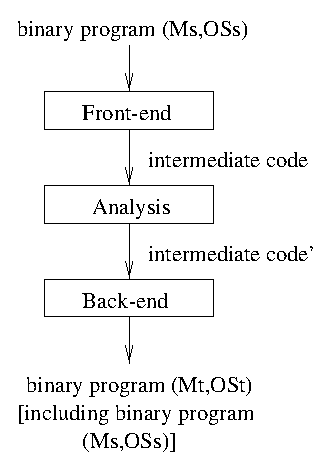
\includegraphics{figures/static.eps}}
\centerfigend{fig-static}{Structure of a static binary translator for
	source machine $M_s$, target machine $M_t$, source operating system
    $OS_s$ and target operating system $OS_t$.}
 
The fallback mechanism used by static binary translators is a runtime
environment that completely supports the source platform, and
hence includes an interpreter for source machine instructions, and support
for translation and mapping of operating system calls into the new
platform.  The development of a runtime environment is a significant
overhead; especially the mapping of operating system calls.  There is
little performance data reported in the literature regarding the amount of
time spent by binary translated applications in the interpreter mode.
Code ported from a proprietary CISC to RISC machine at Tandem, where the
operating system was binary translated to the new machine, reports an
average figure of 1\% of the time being spent on interpretation~\cite{Andr92}.
Informal talks with people who have developed such translators state that
the interpretation mode is seldom used if you have sufficient coverage 
of the patterns generated by compilers commonly used in that platform. 
Existing static translators have dealt mainly with procedural code, 
rather than object-oriented code, which poses new limitations to static
translation due to their dynamic nature of code dispatching through 
vtables.  
 
 
\subsection{Dynamic binary translator}
A dynamic binary translator performs the translation of the code while 
the program is being executed by the translator; that is, the input 
binary program is dynamically analyzed and translated into the target 
machine code during runtime.
Dynamic translation techniques overcome some of the shortages of static
translation, for example, determining the targets of indirect jumps.
Dynamic translation is able to support most practical cases of 
self-modifying code; code normally not supported in static translations.
Given that all the processing of a dynamic translator is done ``on the
fly'', the types of optimizations and analyzes have to be carefully
considered and optimized so that the minimum amount of time is spent
during runtime.
 
The structure of a dynamic binary translator is depicted in
Figure~\ref{fig-dynamic}\footnote{
Figure~\ref{fig-dynamic} by the SELF team at Sun Microsystems Labs.}.  
The binary program is fed into the front end which generates an 
intermediate representation for a block of code.  This representation 
is then compiled or emulated by the translator to generate
(unoptimized) machine code for the target machine.  If at any time the
translator determines that a new region of the program needs to be decoded,
the front end is dynamically invoked to parse that region and provide the
intermediate representation.  When generating machine code, counters are
kept on the number of times blocks of code are executed; once a threshold is
reached, machine code is regenerated to produce better machine code---this
process can be repeated several times, hence producing better code on a
demand-driven basis.  It is important to note that the translation is done
in a lazy fashion; that is, code is only translated when its path is reached.
In this way, fragments of the program that are not executed during runtime,
are not translated either.  Self-modifying code is handled by
invalidating the existing intermediate representation and re-parsing
the binary code with the changed bytes.
 
\centerfigbegin
\resizebox{!}{6cm}
{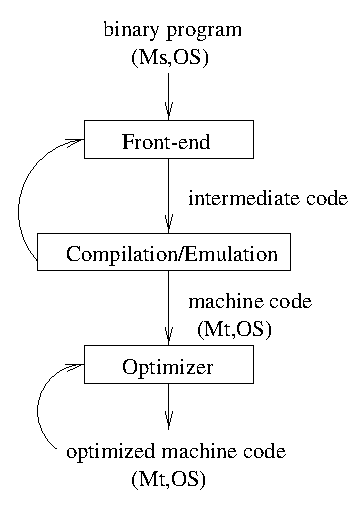
\includegraphics{figures/dynamic.eps}}
\centerfigend{fig-dynamic}{Structure of a dynamic binary translator for
    a source machine Ms, a target machine Mt and a multi-platform
    operating system OS.}
 
Dynamic compilers can perform runtime optimizations of the code based
on the execution profile of the program, hence several optimizations,
such as dynamically-dispatched calls and procedure inlining, can only be
possibly done on a dynamic compiler rather than using static techniques.
The performance penalty of code generated by such a translator is estimated
between 0.9X to 2.4X times that of code generated by a native optimizer
C++ compiler (these figures are based on code generated by the SELF-93 dynamic
compiler~\cite{Holz95}).
 
An interesting point to note is that a dynamic binary translator for
a multi-platform operating system does not require the development of
a runtime environment to support the mapping of old operating system
calls, as all translations are done ``on the fly''.  Using static techniques
in this case will still require a runtime environment to cater for the
interpretation of old machine instructions--dynamic techniques alleviate
the need for this fallback mechanism, but compromise the speed of 
execution of the program at the expense of less analysis and code
quality.
 




	
\chapter{Previous Work}
\label{ch-prevwork}

{\small
\begin{flushright}
Documentation: Cristina [c.1996, 2001]
\end{flushright} 
}

Binary translation is a relatively new field of research, were the
techniques are derived from the compilation, emulation and decompilation areas. 
Nevertheless, the techniques are ad hoc in nature and little has been 
published about them (mainly driven by commercial interests of the parties
involved).  

In this chapter we describe the related work, which we have classified
into two main groups: works related to binary translation and interpreters 
(or emulators), and works related to binary-code manipulation tools that 
may aid in the process.


\section{Binary translators and interpreters} 
Binary translation techniques were developed from emulation
techniques at research labs in the late 1980s.  Projects
like the HP3000 emulation on HP Precision Architecture
computers~\cite{Berg87} and MIMIC, an IBM System/370 simulator on an
IBM RT (RISC) PC~\cite{May87} were the catalist for these techniques.
One of the goals of the HP project was to run existing MPE V binaries
on the new MPE XL operating system.  For this purpose, a compatibility
mode environment was provided, which was composed of two systems:
a HP 3000 emulator and a HP 3000 object code translator.  The emulator
duplicated the behavior of the legacy hardware, and the translator
provided efficient translated code which relied on the emulator
when indirect transfers of control where met.

Tandem developed an object code translator for TNS CISC binaries
to TNS/R (RISC) in order to provide a migration path for existing
vendor and user software~\cite{Andr92}.  This approach allowed
them to market their new RISC machines years earlier than if no
migration path was available.  Part of the rationale for the
project was also the fact that no reprogramming was involved and
that the techniques would provide faster code than emulation
techniques.  Less than 1\% of the time was spent on emulation.

Digital developed two translators, VEST and mx, to provide a migration
path from their OpenVMS VAX and Ultrix MIPS systems to their new
Alpha machine~\cite{Site92,Site93}.  Interestingly enough, they
decided to do careful static translation once instead of on-the-fly
dynamic translation at each execution time for performance issues.
In both their translators, the old and new environments were, by
design, quite similar, plus both provided similar operating system
services.  Some of the goals were to take full advantage of the
performance capabilities of the Alpha and avoiding the problem of
not having all the tools available to port a program to a new architecture
(because they are still not available on the new hardware).
This was seen as an interim solution, while the user's environment was
made available on the new machine and then code could be recompiled/rebuilt.

Up to 1992 all translators were made available by hardware                   
manufacturers to provide a migration path from their legacy
hardware platform (normally a CISC) to their new platform
(normally a RISC).

Back in 1994, AT\&T Bell Laboratories provided services to migrate
software in object code form from one platform to another through
the FlashPort binary translator~\cite{Att94}.
Translations of PDP 11, 680x0 and IBM 360 code was made to
platforms like MIPS, RS/6000, PowerPC and SPARC.  Translation
time was based on the type of application, with some large
applications being translated in 1 month, whereas others in
6 months; which means that manual changes were done to assure
consistency of the translation, plus to provide compatibility
libraries to cater for the differences in operating systems and
services.
The FlashPort technology was initially developed by Bell Laboratories
researchers and was commercialized through the 1991-formed Echo
Logic company.  The first production release of the technology
was provided to Apple Computers in 1993 to translate Macintosh
binaries to the then forthcoming PowerPC-based Macintosh computers.

In an attempt to make Alpha machines more appealing to existing
Unix users, Digital released FreePort Express, a SunOS SPARC
static binary translator to Digital Unix Alpha~\cite{Dec95};
particularly at a time when Sun was migrating customers to
their new Solaris OS and discontinuing support for SunOS.
The tool was advertised as a way of migrating to the Alpha even
when source code and compiler tools from the source machine
were not available; then do a native port at your own leisure.
Since the translated programs and libraries provided support for
Xview, OpenLook, Motif and other X11-based applications, this
migration path was suitable for users who did not want to be
trained in the use of new tools.

To improve Alpha's usability as a desktop alternative to Intel
PCs, Digital developed FX!32, an WindowsNT x86 to WindowsNT Alpha
translator~\cite{Thom96,Hook97}.  Emulation was used as it provided
a quick way to provide support for changes in WindowsNT.  However,
binary translation on the background was also used in order to
save the translations to a file and, over time, incrementally
build the new Alpha binary.  This hybrid translator uses profiling
information in order to optimize the code the next time it
is run.

The TIBBIT project looks at real-time applications that are to be
binary translated between processors of different speeds~\cite{Cogs95,Cogs95b}.
The translated software needs to retain the implicit time-dependency
of the old software in order to function correctly.

\begin{table*}[hbtp]
{\footnotesize
\begin{tabular}{|p{1.5cm}|p{1.3cm}|p{0.7cm}|p{5cm}|p{2cm}|p{2cm}|} \hline
Name & Affiliation & Ref & Purpose & Source Platform & Target Platform \\ \hline
Bergh et al (1987) & HP & \cite{Berg87} &
	Software emulation and object code translation. &
	(HP3000, MPE V) &
	(HP Precision Architecture, MPE XL) \\
Mimic (1987) & IBM & \cite{May87} &
	Software emulator with a 1:4 code expansion factor per 
	old machine instruction. &
	IBM System/370 &
	IBM RT PC \\
Johnson (1990) & Stardent & \cite{John90} &
	Postloading optimizations. &
	RISC &
	RISC \\
Bedichek et al (1990) & U.Wash & \cite{Bedi90} &
	Efficient architecture simulation and debugging. &
	Motorola 88000 &
	Motorola 88000 \\
Accelerator (1992) & Tandem & \cite{Andr92}        &
	Static binary translation for CISC to RISC migration.  
	Uses a fallback interpreter.    &
	TNS CISC        &
	TNS/R   \\
VEST, mx (1993) & Digital & \cite{Site93} &
	Static binary translation from Digital's VAX and MIPS machines
	to the 64-bit Alpha.  Uses a fallback interpreter. &
	(VAX, OpenVMS), (MIPS, Ultrix) &
	(Alpha, OpenVMS), (Alpha, OSF/1) \\
Wabi (1994) & Sun & \cite{Sun94} &
	Pretranslated Windows API to Unix API calls.  Dynamic execution of 
	programs. &
	(x86, Windows 3.x) &
	(SPARC, Solaris) \\
Flashport (1994) & AT\&T & \cite{Att94} &
	Binary translation across a variety of source and target platforms.
	Requires human intervention. & 
	680x0 Mac, IBM System/360, 370, 380 &
	PowerMac, IBM RS/6000, SPARC, HP, MIPS, Pentium \\
Shade (1994) & Sun & \cite{Cmel94} &
	Efficient instruction-set simulation and trace generation
	capability.  Dynamic compilation of code. &
	SPARC V8, V9 &
	SPARC V9, V8 \\
MAE (1994) & Apple & \cite{Apple94} &
	Macintosh environment in an XWindow, Unix RISC-based workstation. &
	680x0 &
	RISC-based Unix \\
Wahbe et al (1994) & CMU & \cite{Wahb94} &
	Adaptable binaries.  Binary transformations.&
	(MIPS, Ultrix4.2) &
	(MIPS, Ultrix4.2) \\
Chia (1995) & Purdue & \cite{Chia95} &
	Software emulation within the same platform, with a 1:100 code
	expansion factor per old machine instruction. &
	(SPARC, Solaris) &
	(SPARC, Solaris) \\
TIBBIT (1995) & CMU, UO & \cite{Cogs95,Cogs95b} &
	Binary translation of time-sensitive applications.&
	Motorola 68000 &
	(IBM RS/6000, AIX 3.2) \\
Then (1995) & Purdue & \cite{Then95} &
	Optimization of code within the same platform.&
	(SPARC, Solaris) &
	(SPARC, Solaris) \\
Freeport Express (1995) & Digital & \cite{Dec95} &
	Static binary translation and fallback interpreter.  Translates
	user mode programs. 32-bit to 64-bit translation. &
	(SPARC, SunOS4.1.x) &
	(Alpha, OSF/1) \\
FX!32 (1996) & Digital & \cite{Thom96,Hook97} &
	Hybrid emulator/binary translator of popular x86 32-bit applications 
	to Alpha.   &
	(x86, WindowsNT) &
	(Alpha, WindowsNT) \\
\hline
\end{tabular}
\caption{\label{tab-bintrans} {Summary of Binary Translators and
	Interpreters in Cronological Order.}}}
\end{table*}

We summarize the features of a variety of binary translators and
interpreters in Table~\ref{tab-bintrans}.  The column {\em Purpose\/} 
describes the general use of the tool, columns {\em Source Platform\/}
and {\em Target Platform\/} describe the nature of the translation supported
by the tool (i.e. multi-platform or within the one platform), 
column {\em Name\/} refers to the name of the software; if unnamed, then
it refers to the people that worked on it, and column {\it Affiliation}
refers to the affiliation of the authors of the software at the time
of development. 


\subsection{List of recent translators}
There has been a lot of work in the last few years (1998-2000) 
on dynamic techniques for doing binary manipulation of one sort of 
another.  The following is a list of projects and literature available: 

\begin{itemize}
\item HP Aries~\cite{Zhen00}: 
Aries is a hybrid interpreter/dynamic translator which
allows PA/RISC HP-UX binaries to run in an IA-64 HP-UX
environment transparently, without user intervention.

\item HP Labs Dynamo~\cite{Bala00}: 
Dynamo is a dynamic reoptimizer of PA-RISC binaries which
produces PA-RISC code.  It works well for some programs 
and not for others. 

\item IBM TJ Watson Research Center's DAISY~\cite{Ebci96} and 
BOA~\cite{Gsch00}: 
The DAISY and BOA projects have looked at dynamic binary translation 
from conventional architectures such as the PowerPC to VLIW or other
novel architectures.  Their work addresses precise exceptions, 
self-modifying code, and reordering of memory references; all of 
these from an architectural point of view. 

\item Transmeta's Crusoe~\cite{Gepp00}: 
The Crusoe chip is a VLIW chip which includes code morphing to 
dynamically binary translate from x86 to the VLIW instruction set. 
Some x86 instructions are supported by the hardware itself. 

\item Compaq's Wiggins/Redstone~\cite{Reev00}: 
Wiggins/Redstone was a dynamic reoptimizer of Alpha binary code. 
It was built based on Digital's DCPI infrastructure.  

\end{itemize}



\section{Binary-code manipulation tools}

\begin{table*}[hbtp]
{\small
\begin{tabular}{|p{2.0cm}|p{0.7cm}|p{7.8cm}|p{3.0cm}|} \hline
Name & Ref & Purpose & Platform \\ \hline
Silberman et al (1993) & \cite{Silb93} &
	Framework for supporting heterogeneous instruction set architectures. &
	CISC, RISC, VLIW \\
QPT (1994) & \cite{Laru94} &
	Rewrite executable files to measure program behavior. &
	MIPS, SPARC \\
Shade (1994) & \cite{Cmel94} &
	Execution profiling of application binaries. &
	SPARC V8, V9 \\
ATOM (1994) & \cite{Dec94,Eust95} &
	Sytem for building customized program analysis tools. &
	(DecStation, Ultrix), (Alpha, OSF/1) \\
NJMC (1994) & \cite{Rams95,Rams94,Rams97} & 
	Machine-independent encoding and decoding of machine instructions
	via the SLED language. &
	MIPS, SPARC, x86, PowerPC, Alpha \\
EEL (1995) & \cite{Laru95} &
	Library for editing binaries. &
	MIPS, SPARC \\
\hline
\end{tabular}
\caption{\label{tab-bintools} {Summary of Binary-code Manipulation  
	Tools in Cronological Order.}}
}
\end{table*}

Table~\ref{tab-bintools} summarizes the available tools for handling
machine binary code.  The column \emph{Name} lists the name of the
tool (or its author if no name was given to the tool), column 
\emph{Ref} lists the references in the literature to this tool,
column \emph{Purpose} describes the purpose of the tool, and column 
\emph{Platform} lists the platform(s) supported by these tools. 

ATOM is a tool-building system that provides a flexible and efficient
interface for the instrumentation of code and has been used for the
construction of an instruction profiler, cache simulator and compiler
auditing tool~\cite{Eust95}.  The user needs to write an instrumentation
file in terms of ATOM's abstractions (procedures and basic blocks),
and an analysis file (using a high-level language such as C) with the 
routines that are to be included for instrumentation purposes.  
The performance of the generated tools compare favourably with 
hand-crafted implementations of same the tools. 

Shade is an instruction-set simulator which optionally allows users to 
profile code that traces the execution of an application at runtime.  
Trace information on instruction addresses, instruction text, decoded
opcode values, and more can be collected by Shade~\cite{Cmel94}.
This tool works only on SPARC machines.

Both NJMC (New Jersey Machine-Code) toolkit~\cite{Rams95,Rams97} and EEL
(Executable Editing Library)~\cite{Laru95} provide support for
manipulating machine instructions.  The NJMC toolkit supports the 
encoding and decoding of machine instructions for a variety of 
RISC and CISC machines, by means of SLED specifications.  
The SLED language allows for the description of the syntax of machine 
instructions in a specification that resembles instruction descriptions 
found in architecture manuals.
The toolkit has successfully been used in a retargetable 
linker~\cite{Fern95} and a retargetable debugger~\cite{Rams92}.  
The EEL library was built based on the NJMC machine specifications, 
and introduced control flow support based on techniques developed in 
the QPT~\cite{Laru94} profiler.  EEL also introduced limited
support for describing the semantics of machine instructions.
The tool is not fully portable to non RISC environments.




	
\chapter{The UQBT Framework}
\label{ch-uqbt-framework}

{\small
\begin{flushright}
Design: Cristina, Norman; Documentation: Cristina [c.98, May 00, Nov 01]
\end{flushright} 
}

The University of Queensland Binary Translator (UQBT) 
framework, is designed to support experimentation in static
binary translation.
UQBT strives to adapt easily to changes in both source and
target machines at low cost, including translations to
register-based and stack-based machines.
Support for multiple architectures is provided by means
of specification of properties of machines, as well as 
conventions used by operating systems.  
This chapter describes the overall architectural organization
of \uqbt\ (Section~\ref{sec-arch}) and its components from the point of view 
of instruction translation (Section~\ref{sec-framework}).  Note that
these two sections are necessarily overlapping; the former
section reflects more of the design and the latter section
reflects more of the implementation of the system.  
The chapter concludes with a small section on the state of the
UQBT framework at the end of 2001. 


\section{The Proposed 1997 Architecture of a Retargetable Binary Translator}
\label{sec-arch}

Like a compiler and a decompiler, a binary translator can logically
be divided into three phases: front end, analysis and transformation,
and back end.  For a given source machine M$_s$ and destination machine M$_d$,
the front end decodes machine M$_s$'s binary file and stores the 
information in a machine-independent intermediate form based on RTLs.
The analysis phase maps machine M$_s$'s locations onto machine M$_d$'s 
locations and transforms the RTLs so that they can be readily translated into 
native code for machine M$_d$.  The back end translates the intermediate 
form and writes a binary file for machine M$_d$.  It may also optimize 
instructions.

From a retargetability point of view, it is more helpful to think of 
a functional division into components instead of a sequential division 
into phases.  Such components may be used in more than one phase.
Some components will be machine-independent; others may be generated 
from machine descriptions.  In Figure~\ref{fig-architecture}, we identify 
components by putting them in boxes.

% original file created in Visio, printed to a file using Adobe's Default
% Postscript Printer driver (option EPS), and crop with ghostview (gsview 
% on the PC version 2.5) using File->PStoEPS option.
\centerfigbegin
\resizebox{!}{10cm}
{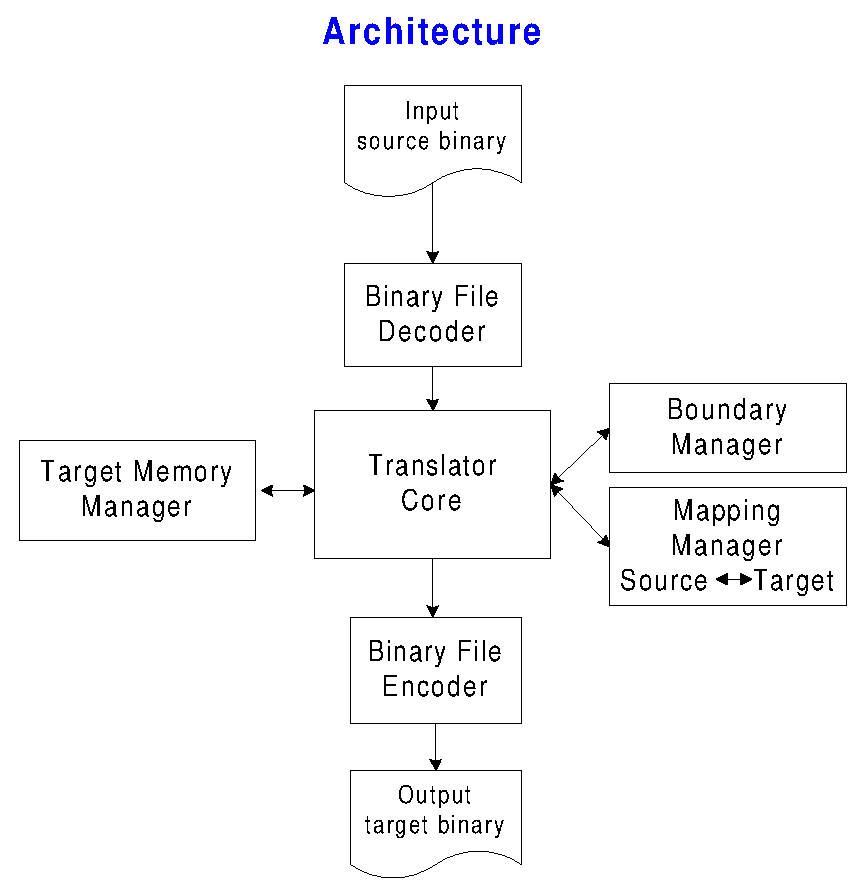
\includegraphics{figures/uqbt_architecture.eps}}
\centerfigend{fig-architecture}{Architecture for a Retargetable Binary
	Translator.  Components are Represented in Boxes.}

Implementation of components draws on techniques developed for
dcc, an 80286 decompiler~\cite{Cifu95}, for specifying
representations of machine instructions~\cite{Rams97},
and for the U.S. National Compiler Infrastructure project.


\subsection{Components}

M$_s$ \emph{binary file reader} exports an abstraction
representing the contents of the executable binary on the original
machine.  This module promotes retargetability by hiding
information about the source machine that one might otherwise be
tempted to exploit.  The capabilities exported include:
%\enumerateAlpha
\begin{enumerate}
\item The initial state of the M$_s$ processor that would apply when about
     to run this binary on a native M$_s$ processor, including at minimum
     the value of the program counter,
\item A list of potential entry points for procedures, possibly empty
     (N.B. the initial program counter is always available as an entry
     point), 
\item The ability to fetch the program's code and data, by the address
     those contents would occupy in a running M$_s$ executable, and 
\item The ability to identify calls to dynamically linked procedures, and
     to provide access to the code and data associated with those
     procedures.
\end{enumerate}
%\enumerateNumber
This module may therefore include much of the functionality of a dynamic
linker/loader.

One of the crucial decisions made by a translator is which locations
on machine M$_d$ hold what data from machine M$_s$.  We will encapsulate these
decisions in a \emph{mapping manager}, which will map locations in code
space, locations in data space, and locations referring to registers
or other processor state.  Most mappings will be determined
automatically at translation time, but some mappings may be specified
by hand for each pair of platforms, e.g., what registers of machine M$_d$
should be used to represent the contents of registers of machine M$_s$.

The mapping manager will rely on the M$_d$ \emph{memory manager} to allocate 
locations in the destination machine's storage space, e.g., to store 
translated code.

Because it is impossible to identify and translate all code, a running
image on machine M$_d$ will in general have a mix of translated and
untranslated code.  The \emph{boundary manager} will track the boundary
between translated and untranslated code and handle flow of control
across the boundary.  For example, a branch from translated to
untranslated code might go to an interpreter or to a dynamic
translator.  If the untranslated code is subsequently translated, the
boundary moves, and the boundary manager might backpatch the branch.

The \emph{core translator} will translate groups of machine instructions.
A group may be as small as a basic block or as large as an entire 
program, and different translation strategies (e.g., full static, 
partial static, dynamic) may use different group sizes.

The core translator coordinates the action of all the other
components and performs the main translation analyses.  It will 
translate a group of M$_s$ instructions as follows:
%\enumerateAlpha
\begin{enumerate}
\item Ask the memory manager for a location in M$_d$ to hold the translated
     code, and inform the mapping manager of the new mapping, 
\item Translate M$_s$ instructions to M$_d$ instructions
	  \begin{itemize}
      \item using information from the mapping manager to translate
         access to machine M$_s$'s data, 
      \item using information from the boundary manager to translate flow
	  \end{itemize}
	 of control outside the current group, and
\item Inform the boundary manager of the translation of the current group.
     The boundary manager may choose to backpatch branches into the
     current group.
\end{enumerate}
%\enumerateNumber
Depending on the granularity and timing of translation, these steps may
be repeated on other units until some termination condition is met.
If the granularity of translation is sufficiently large, the second step
may involve translating into an intermediate form and doing some global
analysis and optimization.

Finally, the M$_d$ \emph{binary file writer} will export an abstraction
representing the ability to create an executable binary on machine M$_d$.
It will export the abilities to:
%\enumerateAlpha
\begin{enumerate}
\item Specify the contents of the M$_d$ address space at the start of
     execution,
\item Establish the state of the M$_d$ processor at the start of execution,
\item Write an executable binary file in the M$_d$ native format, and
\item Possible support for dynamic linking, e.g. of translated or native
     libraries.
\end{enumerate}
%\enumerateNumber
In a dynamic translator, this component would simply write into a
running process image (and possible flush the I-cache).


\subsection{Core Translation based on RTLs}

The translation itself will be performed using register transfer lists
(RTLs).  An RTL is a collection of simultaneous effects.  Each effect
has the form `location := expression', and the expression is always
evaluated without side effects, so all state change is explicit.  
RTL expressions are represented as trees, the leaves of which refer to
constants or to the values contained in locations.  Note that although
the tree leaves refer to locations, the values themselves are not
necessarily calculated, only the location is referenced.
The internal nodes of the trees are `RTL operators'.  
For illustrative purposes, the following is an ASCII representation of an 
RTL representing the effect of the SPARC \texttt{andcc} instruction:
\begin{smallverbatim}
 $r[rd] <--      and (*$r[rs1], if i = 0 then *$r[rs2] else simm13! fi);
 icc.N  <-- bit (and (*$r[rs1], if i = 0 then *$r[rs2] else simm13! fi) < 0);
 icc.Z  <-- bit (and (*$r[rs1], if i = 0 then *$r[rs2] else simm13! fi) = 0);
 icc.V  <-- 0;
 icc.C  <-- 0
\end{smallverbatim}
This RTL does a bitwise AND of the contents of register rs1, either
with the contents of register rs2 or with a signed immediate value (simm13).
This result is stored in register rd, and it is also used to set two
of the four condition codes.  The other two condition codes are set to 
zero by the instruction.

RTLs are obviously complex and detailed.  Machine descriptions
themselves will be written at a higher level of abstraction and
compiled into RTLs.  Run-time representations of RTLs will be
`collapsed' either by analyzing these higher-level representations or
by using the `superoperator' technique~\cite{Proe95}.  
For example, we might define a superoperator LOGICAL such that LOGICAL(X)
stood for
\begin{smallverbatim}
 $r[rd] <--      X;
 icc.N  <-- bit ((X) < 0);
 icc.Z  <-- bit ((X) = 0);
 icc.V  <-- 0;
 icc.C  <-- 0
\end{smallverbatim}
Such a superoperator could be derived from the SPARC description. 

An `RTL language' is defined by a collection of locations and
operators.  For binary translation, a suitable RTL language can be
defined by taking the union of locations on machines M$_s$ and M$_d$ and the
union of the operators used in the descriptions of machine M$_s$ and M$_d$.
The `machine X invariant' defines a sub-language of RTLs called the
X-RTLs; an RTL is an X-RTL if and only if it can be represented as a
single instruction on machine X.

% original figure in Visio, exported as eps (without including TIFF
% preview or background rectangle).
\centerfigbegin
\resizebox{!}{12cm}
{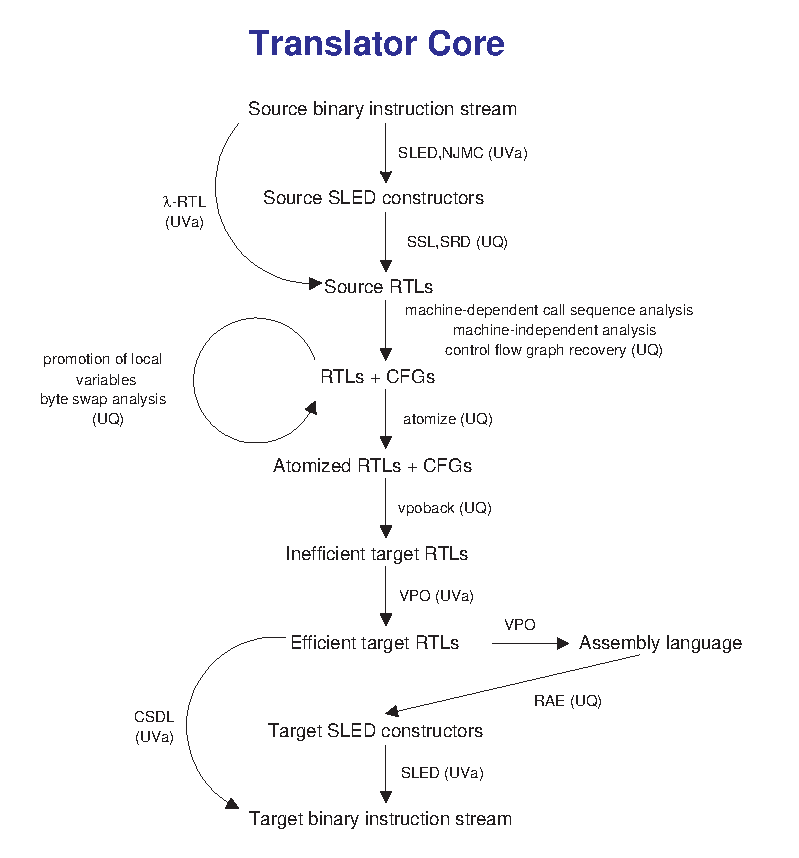
\includegraphics{figures/uqbt_dataflow.eps}}
\centerfigend{fig-dataflow}{Flow of Data through the System}

As shown in Figure~\ref{fig-dataflow}, the main steps in the translation are:
\begin{enumerate}
\item Decode the binary stream into M$_s$-RTLs.  This step will be
     automated by specifying syntax and semantics of M$_s$ instructions.

\item Build a control flow graph (CFG) for each procedure.  Analysis
     will be needed to find code associated with a procedure.

\item With the help of the mapping manager, map the machine M$_s$ locations
     in the RTLs to machine M$_d$ locations or to temporaries.

\item `Atomize' the RTLs to expose all RTL operators at top level, and
     find suitable replacements for machine M$_s$ operators that are not
     available on machine M$_d$.  For example, big-endian memory access
     might be replaced with explicit byte swapping.

\item Reassemble the RTLs to satisfy the machine M$_d$ invariant, making
	them M$_d$-RTLs (i.e. M$_d$-RTLs have a 1:1 mapping with M$_d$ 
	assembly instructions).

\item Optimize the M$_d$-RTLs using VPO~\cite{Beni88} or any other RTL 
	optimizer.

\item Encode the M$_d$-RTLs into binary code for machine M$_d$.  Also automated.
\end{enumerate}

The most challenging steps are steps (4) and (5).  In the initial
stages, these will be implemented by hand; we hope to develop automated
techniques afterwards.  The other steps can be automated based on
machine descriptions or a mapping specification.

Future analyses, intended to improve translated code, might be
implemented after steps (2), (3), or (4).  Such analyses might make it
possible to avoid byte swapping, to use machine M$_d$ calling conventions,
to put machine M$_s$ stack variables in machine M$_d$ registers, etc.
Analyses may vary depending on the granularity of translation.


\section{The 1999 UQBT Framework}
\label{sec-framework}

In order to support resourceability and retargetability, 
machine descriptions of machine properties are needed, 
as well as descriptions of conventions and formats used by 
the operating system.  We have identified 6 different specification 
languages and/or APIs to support the UQBT framework, 4 of these are 
currently in use in our framework. 

The framework described in this section dates from 1998, 
Section~\ref{sec-2001framework} describes the 2001 framework. 
References in this section are to papers and chapters within 
this book that explain in more detail a particular concept. 


\subsubsection*{Machine specifications and APIs} 
Properties of a machine are represented in terms of the machine 
instructions (i.e. the mnemonics), the semantics of such instructions, 
the identification of the instructions that transfer flow of control, 
and, if needed, delayed transfers of control information.  
These 4 types of information are represented by the following 
languages: 

  \begin{itemize}
  \item SLED (Specification Language for Encoding and Decoding), 
	which supports descriptions of the syntax of machine 
	instructions~\cite{Rams97}.  [Chapter~\ref{ch-decoding}];

  \item SSL (Semantic Specification Language), which supports 
	descriptions of the semantics of machine 
	instructions~\cite{Cifu98c}.  [Chapter~\ref{ch-ssl}]; 

  \item CTL (Control Transfer Language), which supports the 
	identification of instructions that perform control 
	transfers of control (conditional jumps, jumps, calls or 
	returns). This language was implemented as a loose API in the
	end, as we decided not to specify other transfer of control 
	information in the end.  

  \item DCTL (Delayed Control Transfer Language), which supports 
	the description of simple transformations needed in 
	order to remove dependencies on delayed instructions (in 
	machines that support such concept).  

    Support for DCTL is not in place at present.  Initially, we used 
    a program-transformation and partial-evaluation technique to derive 
    the transformations on instructions that support delayed transfers of 
    control~\cite{Cifu98i}.  [Chapter~\ref{ch-delay}].
    The code is voluminous and we believe that code to support such 
    transformations could be automated from a short specification 
    of the required transformations.  This step would clearly increase 
    the resourceability of the framework.  However, we note that not 
    too many machines currently support the delayed-slot transfer of 
    control, only SPARC, PA-RISC and MIPS do at present time.

  \end{itemize}


\subsubsection*{OS specifications/APIs} 
Conventions and formats used by a multiplatform operating system come 
in the form of calling conventions, including where parameters are passed 
(i.e. stack or registers), and the format of the binary-file that the 
OS supports.  
These 2 pieces of information are represented by the following 
languages/APIs: 

  \begin{itemize}
  \item PAL (Procedural Abstraction Language), which supports 
	the description of calling conventions, parameter passing conventions, 
	and local variables conventions~\cite{Cifu99g}. [Chapter~\ref{ch-call}];  
	and 

  \item BFF (Binary File Format), which supports the description 
	of the internal format of a binary-file, such as the 
	Elf format on Solaris and Linux systems~\cite{Cifu97f}. 
	[Chapter~\ref{ch-bff}].  
  \end{itemize} 

We currently support the PAL language and have worked on 
an initial prototype of the BFF language, which is incomplete 
at present time but proves the feasibility of specifying 
binary-file formats and automatically generating code to 
support the decoding of such files.  In our experience, it 
was easier to have a set API for dealing with differences in 
binary-file formats than to specify the existing ones.   

\psfigbegin{figures/uqbtImplementation.eps}{10cm}
\psfigend{fig-uqbt}{Framework for a Resourceable Binary Translator.}

Figure~\ref{fig-uqbt} illustrates the components of the 
translation process in the form of boxes.  Specifications for different
machines are illustrated with the document shape.
Greyed-out shapes mean that they are not currently supported 
by UQBT and therefore an implementation for a particular format 
or analysis has been done instead.  Arrows represent conceptual 
flow of control in the translation process.  


\subsection{The Decoding Phase}
The binary-file decoder, instruction decoder 
and semantic mapper translate raw machine instructions into  
M$_s$-RTLs for a given source machine M$_s$.  
As previously mentioned, we consider M$_s$-RTLs machine dependent, as
they represent how the source machine performs a given instruction, 
including delayed-slot semantics for example.  

In static translators, the amount of decoding from this phase 
is limited by indirect transfers of control (i.e. statically,  
it is not always possible to determine the target of an 
indexed jump or an indirect call).  
UQBT includes a slicing-based technique to determine the target
address(es) of indirect transfers of control~\cite{Cifu99c}. 
This technique allows us to decode a larger percentage of the
code than otherwise possible, and is reusable across different 
platforms.  


\subsection{The Analysis Phase} 
The translation of M$_S$-RTLs up to \hrtl\ is 
the most challenging stage of the translator.  As seen in 
Figure~\ref{fig-uqbt}, this translation requires information 
about control transfer instructions, delayed control transfers 
(if any), parameter and calling conventions, and locals and 
stack frame conventions.  
CTL specifications allow us to translate low-level register 
transfers into higher level instructions such as calls and 
returns.  
For example, a CTL specification for SPARC states that a 
jump and link instruction with destination register \texttt{\%o7} 
is a call instruction.  This semantics is not necessarily 
obvious from the SSL description of a jump and link instruction. 
Further, the same instruction using destination register 
\texttt{\%g0} is equivalent to an unconditional jump; this 
too is specified in CTL.  

DCTL specifications will allow us to remove delayed-slot 
instructions in a more machine-independent way.  
At present, as previously mentioned, we implement a program
transformation and partial evaluation technique. 

PAL specifications allow us to recover some of the high-level nature 
of the code, by recovering actual parameters and return 
values for functions, and removing the M$_S$-RTL-specific 
instructions that form part of procedure prologues and 
epilogues, as these are represented in different ways in 
different machines.  The analysis is based on live and 
used parameter and return locations; such locations being
specified in a PAL specification, as well as abstraction to 
an abstract frame pointer (\texttt{\%afp}).  
For example, a PAL specification for the Pentium would specify
that parameters can be passed on the stack and that return 
values go into certain registers (\texttt{\%eax} and top of 
the floating point stack). 
A more detailed description of the analysis is available 
in~\cite{Cifu99g} and Chapter~\ref{ch-call}. 
 
\centerfigbegin
\begin{fnverbatim}
r[tmp] = %sp
r[tmp2] := -120
%pwp = %cwp
%cwp = %cwp + 64
%cwp = (%cwp-1) % NWINDOWS
%sp = r[tmp] + r[tmp2]
r[9] = 69 << 10            v1 = 70656
r[8] = r[9] | 720          v0 = v1 | 720
r[15] = %pc
%pc = %npc
%npc = 0x21780             Call printf (v0, v1)
r[9] = r[30] + -20         v1 = %afp + 100
r[10] = 69 << 10           v2 = 70656
r[8] = r[10] | 736         v0 = v2 | 736
r[15] = %pc
%pc = %npc
%npc = 0x2178c             Call scanf (v0, v1, v2)
r[8] := m[r[30] - 20]      v0 = m[%afp + 100]
r[15] = %pc
%pc = %npc
%npc = 0x10a9c             v0 = Call fib (v0)
m[r[30] - 24] = r[8]       m[%afp + 96] = v0
\end{fnverbatim}
\centerfigend{fig-palEg}{Example of the result of the use of PAL
        specifications to translate SPARC-RTL code (left-hand side)
        to \hrtl\ (right-hand side) in a fibonacci program.}

Figure~\ref{fig-palEg} illustrates 
a snippet of SPARC-RTLs for the \texttt{main} of a fibonacci 
program, and the resultant \hrtl\ code.  As can be seen, 
the RTLs for the procedure prologue were removed (and relevant information
used in the translation), the actual parameters to library functions 
\texttt{printf} and \texttt{scanf} are listed, actual parameters 
were moved to variable locations, local variables are in terms of 
an abstract frame pointer called \texttt{\%afp}, and the return 
value for the call to \texttt{fib} has been determined.   
The example also shows that the call to \texttt{fib} has the
right number of parameters (i.e. one), and that the calls to
the variable argument routines \texttt{printf} and \texttt{scanf} 
each take one extra parameter than expected.  These parameters were passed 
as they were live and were valid parameter locations at the 
call site.  However, when the code is executed, these parameters
will not be used as the library routines would not be expecting
these parameters for processing (i.e. the format string 
in both these routines specifies the number of parameters
required to be processed), therefore producing the right
result at runtime.  

Lifting the level of representation of the code to \hrtl\ 
allows for experimentation with different types  
of binary translation-specific optimizations, such as removing 
some of the byte swaps at loads and stores when machines have  
different endianness, or promoting local variables to registers. 
This is future work. 


\subsection{The Encoding Phase} 
\label{sec-encoding}

\centerfigbegin
\begin{fnverbatim}
void main() {
int v0;
int v1;
int v2;
char _locals[120];

        v1=70656;
        v0=(v1)|(720);
        printf(v0,v1);
        v1=(_locals)+(100);
        v2=70656;
        v0=(v2)|(736);
        scanf(v0,v1,v2);
        v0=*((int*)((_locals)+(100)));
        v0=fib(v0);
        *((int*)((_locals)+(96)))=v0;
\end{fnverbatim}
\centerfigend{fig-cEg}{Example generated low-level C code for the partial
        fibonacci example of Figure~\ref{fig-palEg}.}

The last step in this phase is the translation down to the 
target machine's intermediate representation; M$_T$-RTL in 
the case of register-based machines or \bcode\ in the case 
of stack-based machines.  
The translated code will always require an optimizer to improve 
its quality, therefore, the encoder phase would be equivalent 
to that of an optimizing compiler.  Because we interface 
to existing C optimizing compilers, we generate very low-level 
C code from this step.  Figure~\ref{fig-cEg} shows the 
generated low-level C code for the example in Figure~\ref{fig-palEg}. 
As can be seen, data addresses are not modified, therefore  
a call to \texttt{printf} or \texttt{scanf} takes the same 
memory address as that in the source binary.  

We have successfully interfaced to VPO~\cite{Beni88}, whose register 
transfer list interface is similar to our RTLs, and hence it is simple  
to translate to.  The new VPO interface is part of the Zephyr 
project~\cite{Vpo98}.  
Generating (low level) C allows us to experiment with different 
optimizers, and also is the interface to the stack based backends. 
For generation of code to the Java Virtual Machine (JVM), we 
have written a backend and a bytecode description that 
integrates with gcc. 

\centerfigbegin
\begin{fnverbatim}
                   ... (setup code)
v2=134517960;      ldc 124517960   ; put string in local 10
printf(v2);        istore 10
r24=(_afp)+(4);    aload_0         ; call _printf
v2=r24;            iload 10
v1=134517975;      invokevirtual Fibo/_printf (I) I
scanf(v1,v2);      istore 10
                   ldc 16          ; put afp+4 in local 12
                   lstore 9
                   iload 14
                   iload 9
                   iadd
                   istore 12
                   ldc 134517975   ; put string in local 10
                   istore 10
                   iload 12        ; put afp+4 in local 11
                   istore 11
                   aload_0         ; call _scanf
                   iload 10
                   iload 11
                   invokevirtual Fibo/_scanf(II)I
                   istore 10
\end{fnverbatim}
\centerfigend{fig-bcodeEg}{Example of generated bytecode after gcc
        optimizations (right-hand side) for low-level C code
        generated from Pentium fibonacci binary (left-hand side).}

The generation of bytecode via gcc provides us with all the
classical optimizations that are too computationally expensive to be
performed by a just-in-time compiler.  
We wrote a bytecode specification file for gcc which treats registers 
as locals and describes peephole optimizations.  
For each \hrtl\ instruction, $n$ bytecode instructions are 
generated, where $n$ is normally less than 5.  The generated
bytecode is similar to that generated by a Java compiler, 
given the high level of abstraction of the \hrtl\ code.  
Current work under development improves on the generated bytecode 
by using an intermediate language called \bcode, which allows 
for stack-based optimizations to be performed, therefore minimizing the 
amount of loads and stores from memory and using the stack 
for temporary values more. 
Figure~\ref{fig-bcodeEg} shows sample bytecode generated from our 
gcc bytecode backend.  Library calls are to wrapping routines 
which invoke the native Java library subsystems.  For variable
argument routines, we have $n$ different wrappers, where $n$ is
the number of parameters and typically $n$ is less than 10. 

For each translation, the generated code and data are 
placed into a variety of C and assembly files which can be 
compiled with gcc and gas on the target machine.  
For each function, a low-level C file is generated. 
For each data section, an assembly file is generated with the  
relevant bytes. 
A makefile is provided to pack the file into an appropriate 
binary for the target machine.

Static translators require the use of an interpreter/emulator to handle 
untranslated code that is discovered at run time.  
The interpreter uses the M$_S$-to-M$_T$ mapping to determine when 
it can return to translated code, and therefore this mapping is stored 
in the target binary.
Because the interpreter will use the original source text section, 
this section is also copied to the target binary.
The interpreter itself is designed to be linked dynamically.
We are currently building a resourceable interpreter/emulator which uses 
the same SLED and SSL specifications provided by the UQBT framework.
The interpreter simulates M$_s$-RTLs and uses PAL specifications 
to determine how to pass parameters to library routines.  
This work is not completed at present time and is under development.

Because of potential aliasing problems, not all of which can be solved by
static analysis, the data sections (generally .rodata and .data in 
Elf binary files) are copied ``as is'' to the target binary. 
They are made to retain the same Virtual Memory Address in the 
target binary as in the source binary. A link map file generated by 
the translator is used to achieve this. The target program calculates 
addresses exactly as the original source program did, and so the data 
is referenced correctly (although it may need to be referenced 
using different endianness). 
Because of differences in size of pages in various architectures 
(e.g. 4Kb on Pentium, verses typically 8Kb on SPARC), this mapping 
cannot always be achieved entirely by manipulation of addresses in the 
target binary file. A very small piece of code sometimes has to perform block 
moves (before the normal startup code) to achieve the correct addresses.

Translators to bytecode require extra environment support
to compliment the strengths of the JVM.  The lack of a generic memory
model on the JVM forces us to emulate the data and stack of a translated
program.  Library functions from the source architecture must also be
supplied to the translated program.  This is facilitated by a superclass
from which each translated program is inherited.  The superclass provides
simulated memory access in preloaded byte arrays and wrapper routines to 
library functions which invoke the native Java subsystems.


\section{The 2001 UQBT Framework}
\label{sec-2001framework}

\psfigbegin{figures/uqbtOverall2001.eps}{10cm}
\psfigend{fig-uqbt2001}{The 2001 UQBT Framework}

The final UQBT 2001 framework provides for several backends that 
were written for experimentation with different ways of generating 
machine code, by integrating at different levels of abstraction. 
Figure~\ref{fig-uqbt2001} shows this framework, we briefly describe
its components next.  In the below description, we divide the framework 
into two sections, the front end and the back end.  The former transforms
binary code to the \hrtl\ representation, the latter transforms down 
from \hrtl\ into another binary representation.

\begin{description}
\item Front end: 
We have one resourceable front end which takes 3 machine and OS 
descriptions and 2 APIs, along with any extra machine-dependent 
code to abstract M$_s$-RTLs into \hrtl\ code.  The parts of the 
front end are: 

\begin{itemize}
\item Binary-file decoder: supports the decoding of the source 
	binary file into an internal UQBT representation that supports 
	the binary-file format API.  The API assumes we can obtain the 
	code (text) and data sections of the file, that there is at 
	least one entry point, and that there may be a symbol table.  

\item Instruction decoder: supports the disassembly of the instruction 
	stream (the text/code section(s)) via the SLED specification for
	the instruction set for the source machine being used.   

\item Semantic mapper: supports the conversion of assembly instructions 
	into RTL instructions, by implementing support for the SSL language, 
	which describes the semantics of assembly instructions. 

\item M$_s$-RTL to \hrtl\ translator: this is the key module in the
	framework that allows us to obtain machine independence in the 
	representation of the code of the program.  This module transforms 
	RTL instructions into \hrtl\ instructions, by supporting an 
	informal control transfer API, performing analyses on procedural  
	information (such as parameters, locals and return locations), 
	and adding any extra hand-written code to support peculiarities 
	of the source instruction set; such as delayed branches on SPARC 
	or floating point stack-based instructions on x86.    
\end{itemize}

The net result of the front end phase is to transform the source 
binary's code into a \hrtl\ representation which is machine independent. 
Transformations on this representation are feasible in order to, 
for example, reduce the number of byte swaps needed when translating 
to different endianness machines.  Transformations of this kind are 
considered binary translation-specific optimizations, as a traditional 
compiler optimizer would not have to deal with them at all.  

\item Back end: 
We have experimented with four different types of back ends.  These 
back ends have commonalities which could be extracted into a common 
back end that supports generation of code at different levels of 
abstraction (such as RTL, assembly or object code).  The back ends are:  

\begin{itemize}
\item C back end: the C backend was the original back end we wrote 
	for the UQBT framework that supported several target platforms 
	(we had earlier experimented with an RTL optimizer).  
	In essence, the C compiler was used as a macro assembler.  
	We translated \hrtl\ code into low-level C code; 
	i.e. code that makes use of goto's and performs a lot of casting 
	of types of expressions.  The generated low-level C code would then 
	be compiled and optimized by the C compiler (we normally compiled 
	using GNU's gcc as well as Sun's cc compilers) and then linked 
	against the original data sections of the source program.  The data 
	sections were always forced to be located at the same memory address 
	space as in the original source program.  

\item JVML back end: the Java bytecode (Java virtual machine language (JVML)) 
	back end was written as an experiment in translating machine code to 
	Java bytecodes.  We translated \hrtl\ code into Java bytecode assembly 
	code, which would be assembled by the Jasmin assembler in order to 
	generate a Java binary (.class file).  Some runtime support was needed 
	as the JVM model is different to that of traditional machines; there 
	was support for dealing with memory, allocating and deallocating memory, 
	as well as support for 32-bit integrals (all integers in the JVM model 
	use 31 bits and are meant to be signed).

\item RTL back end: the RTL back end was an experiment at having more 
	control over the optimizations that were applied to the generated 
	code, as by generating RTL instructions for the target machine, 
	we could then tell an RTL-optimizer to only use certain optimizations 
	and to not move around code in certain sections.   We used the 
	VPO~\cite{Beni88} system for this purpose.  VPO is a retargetable 
	optimizer that now provides an RTL interface to it.  VPO makes use 
	of specifications to describe the syntax of the target instructions, 
	has a series of optimizations that are machine independent, and 
	requires the user to write machine dependent optimizations to support 
	any new machine.  

\item Object code back end: the object code back end was written as an 
	experiment to interface with an optimizer at the object code level, 
	i.e. without having to generate any particular intermediate 
	representation.  The generated code would not do register allocation 
	of any sort, instead, it would place all locations (variables and 
	registers) onto the local stack of a procedure, and would rely on 
	the optimizer to perform register allocation.  This was an internal 
	Sun experiment that made use of a proprietary optimizer, as such, 
	the code is released in the event that it is useful to others, but
	the code for the optimizer is not made available (you can potentially
	interface with any optimizer you see fit).   
\end{itemize}


\end{description}





\part{The Frontend}
\label{part-frontend}

	
\chapter{The BinaryFile and ArchiveFile classes}
\label{ch-bff}

{\small
\begin{flushright}
Design: Cristina, Mike; Documentation: Cristina, Mike; Implementation: Mike
[c.1997]
\end{flushright}
}

The term "loader" is generally used to describe a system program
used by an operating system (OS) to load a
binary executable file onto memory to execute it. 
We have a class called "BinaryFile" that can be used by application
programs to load other binary files for purposes other than directly
executing them. (The class was formerly called "Loader", but this
contrasts with the use above).
In other words, BinaryFile is a decoder of binary-file formats; it 
reads a binary executable file and stores its representation in memory,
providing functions to access the different parts of the binary
file; such as code and data.  
It provides extra functionality in the presence of 
dynamically linked-in procedures; binary-file formats such as
ELF and PE (Portable Executable) support them.  In this case,
the BinaryFile interface provides a way of determining if a 
procedure address is an address for a dynamically linked-in 
procedure, and if so, it allows access to its code and data.
In this regard, the BinaryFile class is more of a dynamic linker/loader.

Binary files vary widely in internal organisation and structure,
nevertheless, they provide similar kinds of information 
in order to run the program.  
The main components of a binary file are its code and its data;
everything else is a representational structure to access this
information.
By means of the BinaryFile and ArchiveFile classes, we attempt to 
provide a uniform interface for the loading and usage of the 
information stored in binary files.

Some binary file of interest are collected in library or archive
files. The members of the archive are usually object (.o) files;
there is usually a symbol table associated with the archive so that
the member containing the symbol can readily be found. Archive
files are obviously used rather differently than other binary files
(executable and object files), despite attempts to unify them (e.g.
in the elflib library). Therefore, functions for using archive
files are separated into their own class, called ArchiveFile.
(In the previous form, class Loader had a function GetNextMember
to move to the next member of an archive). When a member of the
archive is selected (by index, or procedure name, or file name),
a reference to an instance of a  BinaryFile class is returned, and all the
BinaryFile functions can be called (except for Load; the BinaryFile
object comes "preloaded").


\section{Related Work}
We briefly describe the two main pieces of related work in this
area.

\subsection{GNU's Binary File Descriptor Library}
GNU's Binary-File Descriptor (BFD) Library~\cite{Cham91} is a package
containing common routines that applications can use regardless of 
their underlying binary-file format.
The BFD library divides each specified BFF into the front-end and the
back-end.
The front-end interfaces between the user and the BFD, while
the back-end provides a set of calls which the BFD front-end can use to
decode and manage the object file.
To support a new BFF, the programmer needs to create a new BFD back-end
and add it to the library.
 
BFD has its own binary representation for internal processing known as the
canonical object file format.
When an binary file is opened, the front-end BFD routines automatically 
determine the format of the input file.  A descriptor is built in memory 
with information about which routines are to be used to access
elements of the binary file's data structure.  When the program wants
information about the binary files, the BFD reads from different sections of
the file and processes them.  Each BFD back-end will have routines to convert
section representations of the binary file to BFD's internal canonical
object-file format.
 
The BFD library is provided to the user as a library.  This library
is fairly large; the number of functions offered in the front-end 
are exceptionally many.
The BFD front-end was designed in mind to allow programmers to
be able to retrieve all types of information about \emph{any} BFF; at
least the existing ones at the time.
Due to its generality and bulkiness, it is difficult to use without
spending a big overhead on learning how to use it.
Perhaps because it is too general, it often contain more information 
than is needed for particular system applications.
 

\subsection{SRL - A Simple Retargetable Loader}
SRL, a simple retargetable loader, is a first attempt at developing a 
retargetable loader framework by means of a simple BFF grammar~\cite{Cifu97f}.  
Three different environments, (x86,DOS,EXE), (x86,Windows,NE) and 
(Sparc,Solaris,ELF), were used as the basis for the development and 
testing of SRL.  The three environments gave a good coverage of different 
BFFs currently in use by OSs for RISC and CISC machines. 

The BFF grammar provides support for describing sections of
the binary file, and to name different fields from each section.
Further, it provides support for structures which have been
stored as a sequence of records of a given type, e.g. the number of
elements in the segment table on the NE (New Executable) format,
by means of an array construct -- this construct clearly aids in
the specification of BFFs.

The EBNF for this grammar's syntax is provided in Figure~\ref{fig-bffg}.  
In the grammar, {\it non-terminals} appear in italics, terminals appear in
normal fontface, ``literal strings'' appear with double quotes, and
\verb!examples! appear in courier.
The start symbol for this grammar is {\it BFFspec}.
Hence, the body for any BFF specification is of the form: \\
{\small
{\it spec} $=>$ {\it format-def defin \{defin\} load-info}
}

\centerfigbegin
{\small
\begin{tabular}{lll}
 {\it BFFspec} & $=>$ & {\it \{spec\}}. \\
 {\it spec} & $=>$ & {\it format-def defin \{defin\} load-info} \\
 {\it format-def} & $=>$ & ``DEFINITION'' ``FORMAT'' \\
    & & {\it ident \{ident\}} ``END'' ``FORMAT'' \\
 {\it defin} & $=>$ & ``DEFINITION'' {\it ident} \\
    & & ``ADDRESS'' {\it expression scope-def} \\
    & & ``END'' {\it ident}. \\
 {\it load-info} & $=>$ & ``FILEHEADER'' {\it ident} \\
     & & ``IMAGESIZE'' {\it expression} \\
     & & ``IMAGEADDRESS'' {\it expression} \\
 {\it scope-def} & $=>$ & {\it ident type-exp \{ident type-exp\}} \\
 {\it type-exp} & $=>$ & ``SIZE'' {\it expression} $|$ \\
    & & ``ARRAY'' {\it expression scope-def} \\
    & & ``END'' {\it ident} \\
 {\it expression} & $=>$ & ``('' {\it ident operator expression} ``)'' \\
     & & $|$ {\it ident operator expression} $|$ $\epsilon$ \\
 {\it operator} & $=>$ & ``+'' $|$ ``-'' $|$ ``*'' $|$ ``/'' $|$ ``\^'' $|$ ``\%'' \\
 {\it ident} & $=>$ & ``a''..``z'' $|$ ``A''..``Z'' \{``a''..``z'' $|$ \\
    & & ``A''..``Z'' $|$ ``\_''\} \\
\end{tabular}
}
\centerfigend{fig-bffg}{Binary-File Format Grammar}

SRL, the tool that implements the BFF grammar, was an attempt
to demonstrate the benefit of using a retargetable loader to 
build a machine-code manipulation tool.  SRL was limited in 
a way by its simple grammar which contained a small number of
constructs.  Nevertheless, the BFF grammar was suitable for
specifying most of the sections of the ELF, EXE and NE formats.
SRL generates a C code in the form of a header file (.h) and 
an implementation (.c) file from each parsed file written in
the BFF language.  The header file contains the data structures
needed for the storing of information for a particular
binary file format, and the implementation file provides 
functions for the loading of a file using the structures 
defined in the header file. 


\subsection{Our Approach}
Our approach is different to the two previous ones, as it is more
specific and less retargetable.  We provide an API (via the
BinaryFile class) that 
users must adhere to, but we do not generate code for it automatically
from specifications, nor do we provide for a complete interface
suitable for a large number of binary file formats.  In contrast,
we provide an object oriented abstraction which provides the base
functionality of a loader (regardless of binary file format) in 
an abstract class, and loaders for specific binary file formats 
(e.g. EXE or ELF) inherit from this abstract class and provide new
functionality specific to their format. Similarly, there is an
ArchiveFile class that defines functions for using archive files,
and there are classes derived from this class for the various types
of archive file.


\section{Binary-file formats}
\label{sec-bff}
We briefly describe the abstract format of a binary file.  
Users not familiar with the internal representation of 
binary files who want more detailed information may refer
to the following literature: \cite{Dunc88b,Sun94m,Micr96} and
the web site \url{http://www.wotsit.demon.co.uk} which has a 
compendium of binary file formats.

The general structure of a binary file format (BFF) can be seen to 
be made up by the following abstraction:
\begin{itemize}
\item A header containing general information about the program
and information needed to access various parts of the file.
\item A number of sections holding code and data (raw data).
\item A relocation table containing offsets of relocatable addresses.
\item A symbol table containing information about symbols of the 
	program.
\end{itemize}
Each of these \emph{parts} is given a name respectively: \emph{header},
\emph{sections}, \emph{relocation table} and \emph{symbol table}.
Further, some binary files such as ELF allow for more than one linked
segment to be stored in the one physical file or archive; we refer
to these segments as \emph{members} of the archive.

Most BFFs can be mapped to the general model in Figure~\ref{fig-bffoa};
however, parts are not necessarily stored in that order.
Information regarding the location of sections, symbol tables, etc is
usually identified within the file header.
Nevertheless, some BFFs do not distinguish between these structures; in
the DOS EXE format, the file header contains information about the relocation
table, but there is no information about where the symbol table is stored
(if any), and where data is; there is only one section that embodies all
code, data and symbol table information.
In all cases though, the program's
header will contain enough information to determine the entry point (i.e.
the start of the program's code) in the file.

% Original file in Visio format, on Blimey (in the Drawings directory)
\centerfigbegin
\resizebox{!}{5cm}
{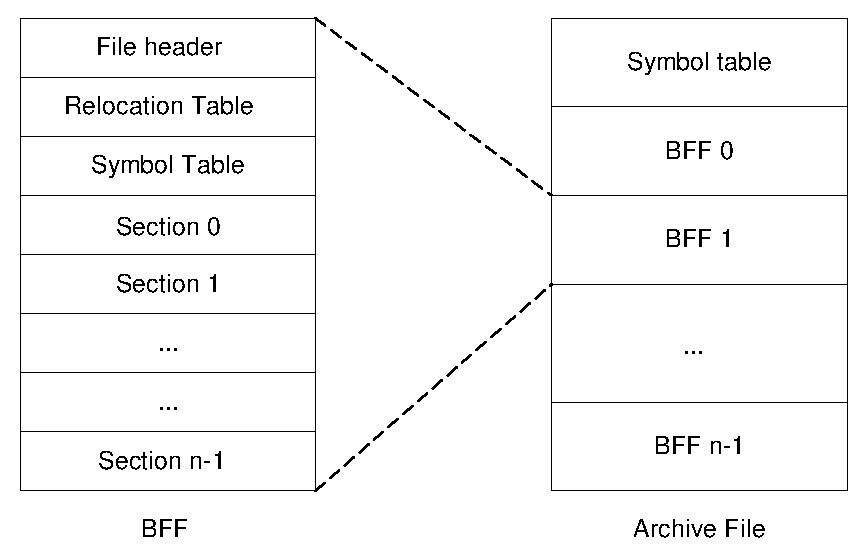
\includegraphics{figures/bffoa.eps}}
\centerfigend{fig-bffoa}{BFF and archive file abstraction}

The current development domain for our tools is based on the Solaris 
ELF~\cite{Sun94m} format, the DOS EXE format~\cite{Dunc88b,Micr96}, 
the Windows (16-bit) NE~\cite{Dunc88b,Micr96} format,
and the Palm OS .prc format~\cite{Tso00}.
Archive files are based on the Unix ar(4) file format.
These formats vary in their degree of complexity and information
stored: the DOS EXE is very simple and limited in structure,
whereas the Solaris ELF format is the most complex, while the Windows
NE is somewhere in between.
The amount of information stored for a simple ``Hello world'' program
varies from format to format.  The DOS EXE format contains a file
header, a relocation table and a single image for both code and data.
The Windows NE version contains most DOS EXE's information plus
additional details such as the resource table, entry table, etc.
The ELF format contains even more information; sections within the 
object file hold information used in dynamic linking: code, data, 
relocation tables, symbol tables, dynamic linking information, etc.
The size in bytes of the binaries for (x86,DOS,EXE), (x86,Windows,NE)
and (Sparc,Solaris,ELF) are 6432, 16384 and 5280 respectively.
It can clearly be seen that although the latter two files are dynamically
linked, their sizes are not necessarily smaller than the static (first)
case.
This is due to the small nature of the example program and the
inclusion of the DOS EXE header information within the NE format.



\section{The BinaryFile Object Hierarchy}
BinaryFile and ArchiveFile are abstract classes; that is, they cannot be
instantiated
directly. The user actually uses classes such as ElfBinaryFile or ExeBinaryFile,
which are derived from the abstract BinaryFile class (see 
Figure~\ref{fig-loadHier}).

% xfig figures exported as eps, portrait, 100% size, displayed at 3.2cm.
\centerfigbegin
\resizebox{!}{3.2cm}
{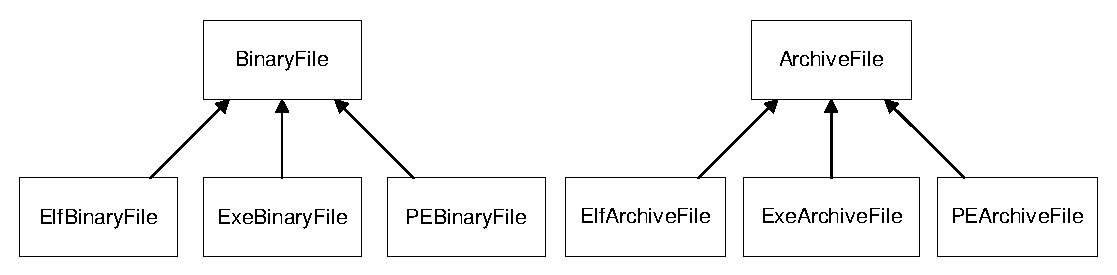
\includegraphics{figures/load_hierarchy.eps}}
\centerfigend{fig-loadHier}{BinaryFile Class Hierarchy}

The user will call functions like \texttt{Load} that are implemented 
differently in the various derived classes. Some functions like
\texttt{SymbolByAddress} are implemented trivially by the BinaryFile class 
(e.g. to always return 0), and this behaviour is overridden by derived 
classes which do the real work.  Even functions like \texttt{GetNumSyms} 
that are implemented by the BinaryFile class will return information that 
will be dependent on the instantiated class.



\section{Interface Functions to Construct and Use a BinaryFile}
The BinaryFile class and each of its parts (described in the abstract 
format description of a binary file in section~\ref{sec-bff}), are 
explained here in terms of interface functions provided for accessing 
information in those parts. 


\subsection{Construction and Loading}
The BinaryFile class provides constructor and destructor 
functions, plus a function to load the binary file.
The loader is an abstract class and hence it does not export 
any types.

\begin{description}
\item [BinaryFile: BOOL $\rightarrow$ BinaryFile].
	This is the constructor. The single BOOL argument is used to
	indicate whether the object to be constructed is to be an
	Archive member; it defaults to false. Users should not use
	this parameter, but should use the ArchiveFile class
	instead (see section~\ref{sec-archive}). The BinaryFile object
	is created without a file loaded; use the Load() function below
	to actually load a file.
	
\item [Load: (BinaryFile x STRING) $\rightarrow$ BOOL].
	Load the given file and store its
	information in a BinaryFile object. It returns whether the
	function was successful or not.
	If there is a problem loading the file, e.g. the file name does
	not exist or there is not enough memory, a message is printed
	on standard error.

\item [UnLoad: BinaryFile $\rightarrow$ nil].
	Deallocates the BinaryFile object. All information about the file
	(e.g. SectionInfo, pointers to section data) are invalid after
	calling this function.

\end{description}


\subsection{Sections}
For each section in the binary file, the following information is 
collected in a SECTIONINFO type:
\begin{itemize}
\item Section name: the name of the section, if any.  Formats like
	ELF support names for each section, such as \texttt{.text} and
    \texttt{.bss}; formats such as EXE do not provide such information
	and hence we follow the convention of naming them \texttt{\.header}
	and \texttt{.text} for the header of the file and the relocatable
	image respectively.

\item Native address: address where the section is logically loaded.
	For example, all EXE files are loaded at address 0x100000,
	representing 10:0000.  ELF files are loaded at the address
	specified in the elf file, typically 0x10000 for code and 0x20000
	for data.  The native address is typically used by diassemblers
	to give a useful address in listing. 

\item Host address: the host address is where the section is actually
	located in virtual memory, i.e. this is a pointer to the first
	byte in the section.

\item Section size: size of the section in bytes.

\item Number of entries: if the section is the equivalent to an 
	array of entries, the size of each entry is given.

\item bCode: This flag is set if the section contains executable
	instructions.

\item bData: This flag is set if the section contains data. It is possible
	for both bCode and bData to be set at the same time.

\item bBss: This flag is set if the section is not initialised, i.e. it
	is for reserving space only.

\item bReadOnly: This flag is set if the section is read only, i.e. it
	cannot be written to.

\end{itemize}

For example, with the ElfBinaryFile class, the section whose name is 
\texttt{\.rodata} would have the flags bData and bReadOnly set.
A disassembler can find all the sections worth disassembling by 
searching through all the sections for those with the flag bCode set.

Sections provide the following functions to determine the number
of sections available in the file and access its information:
\begin{description}
\item [GetNumSections: BinaryFile $\rightarrow$ int].
	Given a BinaryFile object, returns the number of sections that it 
	contains.  

\item [GetSectionInfo: (BinaryFile x int) $\rightarrow$ SECTIONINFO].
	Given an BinaryFile object and a section index, returns the information
	for that section.  Note that sections are indexed from 1.
\end{description}


\subsection{Symbol Table}
Symbol tables are often used for dynamic linking purposes, where
the names of dynamically linked-in routines are stored.  However,
sometimes program symbols are also stored in a symbol table,
whether in the same or a separate table to that of dynamic linking.

The symbol table offered by the BinaryFile class is very simple; 
there are three types of information stored for each entry:
\begin{itemize}
\item Symbol name: the symbol's name in the table.  Type: STRING.

\item Symbol address: the symbol's native address.  Type: ADDRESS.

\item Symbol size: the size in bytes associated with the symbol.
	Type: int.
\end{itemize}

The symbol table offers three access functions to its contents:
\begin{description}
\item [SymbolByAddress: (BinaryFile x ADDRESS) $\rightarrow$ STRING].
	Given a native address, returns the symbolic name associated with the 
	given native address.
	This function is useful when getting names for procedures at
	call locations.

\item [GetAddressByName: (BinaryFile x STRING) $\rightarrow$ ADDRESS].
	Given the name of a symbol, returns the native address associated
	with it.	
	If the symbol is inexistent in the symbol table, an address of 
	0 is returned.

\item [GetSizeByName: (BinaryFile x STRING) $\rightarrow$ int].
	Given the name of a symbol, returns the size in bytes of the 
	symbol, or 0 if inexistent.
\end{description}

Not all BinaryFiles provide the ByName() functions, because in some
cases the binary file format does not support it. If the functions are
not supported, they will always return 0.

Some BinaryFile classes (e.g. ExeBinaryFile) do not implement a symbol table.


\subsection{Relocation Table}
Relocation tables provide information on address that need to be
relocated prior to execution of the program.  
The advantage of knowing which addresses are relocatable is
that when decoding a machine instruction that takes an immediate
operand, we can check if this operand is an address or not. 
This provides us with useful information that is unavailable otherwise.

The functions provided to access the relocation table are:
\begin{description}
\item [IsAddressRelocatable: ADDRESS $\rightarrow$ BOOL].
	Given a native address, returns whether the address is in the
	relocation table or not.

\item [GetRelocatedAddress: ADDRESS $\rightarrow$ ADDRESS].
	Given a native relocatable address, returns the relocated 
	address for it. This function is tentative and not implemented
	as yet; RISC machines require many bit manipulations, and
	this will probably require a different interface function.
\end{description}

With object files, relocations are often associated with symbols.
Sometimes, (e.g. with GCC), intramodule function calls that
could be resolved at compile time are left until link time, so
the call has a relocation entry with an associated symbol table
entry (often not the same symbol table as the main symbols).
To make use of this, the BinaryFile provides this function:

\begin{description}
\item [GetRelocSym: ADDRESS $\rightarrow$ STRING]. Given a
native address, returns a symbol associated with the relocation
at that address, if any. If there is no symbol, the function
returns 0.
\end{description}


\subsection{Program Headers}
Application writers normally like dumping information about 
the headers of the program in order to determine format-specific
information that is not otherwise accessible via the loader
interface.  For example, a loader may have a verbose option to
display this type of information.

Unfortunately, it is difficult to provide a clean interface for
such low level details. (The previous version of the loader
attempted this, but it was not satisfactory). Therefore this
version of BinaryFile provides just one function, for dumping
all the headers in a verbose manner:

\begin{description}
\item [DisplayDetails: BinaryFile x STRING x FILE* $\rightarrow$ BOOL].
	Given a BinaryFile class and the name of the file, sends a verbose
	listing of the
	file to the file indicated by the FILE* parameter.
	The STRING parameter is merely to provide the first line of output,
	which is typically {\it Type} header for {\it Filename}.
	The FILE* parameter can be a special stream such as
	\texttt{stdio}, or a file opened with the \texttt{fopen}
	library function.

\end{description} 

The addresses referred to above are host addresses, i.e. pointers
to actual loaded data. (By contrast, native addresses are those
where part of a file is expected to be loaded in the native
operating system. Headers have no native address.

In the ElfBinaryFile, more specific functions are provided to
access different named headers, such as GetProgramHeader()
and GetSectionHeader().

Given the address of a header, an application writer would have
to know what the contents of the header looks like, and would
have to write the dump function.  We do not consider this
type of detail should be included in our BinaryFile class.


\subsection{Analysis Functions}
The following functions are provided for extra functionality 
required under binary translation, they are:
\begin{description}
\item [GetInitialState: BinaryFile $\rightarrow$ LIST$<$(REGxADDRESS)$>$].
	Returns a list of registers and their initial value (normally
	an address) prior to program execution.

\item [GetEntryPoints: BinaryFile $\rightarrow$ LIST$<$ADDRESS$>$].
	Returns a list of native addresses which are entry points into the 
	program.  The first address is always the initial value of the program
	counter (PC).

\emph{The following function is not implemented at present. It occured to
	me (Mike) that
	the mapping from Native to Host address may vary for each section;
	it doesn't in elf, but it may for other sections. Let's leave this
	one out unless we really need it. It is easy to implement anyway:
	just use the difference between native and host addresses in the
	section info.}
\item [NativeToHostAddress: (BinaryFile x ADDRESS) $\rightarrow$ ADDRESS].
	Given a native address, returns its equivalent host address.
	This function allows access to a block of bytes, since a native
	address is just a pointer.

\item [IsDynamicLinkedProc: (BinaryFile x ADDRESS) $\rightarrow$ BOOL].
	Given a native address, returns whether the address is that of a 
	dynamically linked-in procedure or not in this BinaryFile class.

\item [LoadDynamicLinkedProc: BinaryFile $\rightarrow$ ADDRESS $\rightarrow$ BOOL].
	Given the address of a dynamically linked-in procedure (i.e. the
	target of a call instruction that calls such a function, which
	will usually be an address in the Program Linkage Table), loads
	the appropriate source library file (if needed) to resolve this
	call. It returns its success or otherwise, and the native address
	where the procedure is loaded. 

	There will have to be environment variables to specify what path(s)
	should be searched to locate the appropriate library. These would
	be called \\
	X86\_LIBRARY\_PATH\\
	SPARC\_LIBRARY\_PATH\\
	and so on.  For example,
	if an X86 source program calls the \texttt{atan} function,
	the program's dynamic section specifies the DT\_NEEDED libraries
	as "libc.so.1" and "libm.so.1", and the environment variable
	X86\_LIBRARY\_PATH is set to "/var/lib/x86:/usr/lib/x86", then
	the following libraries will be searched for the \texttt{atan}
	function: \\
	/var/lib/x86/libc.so.1, /var/lib/x86/libm.so.1,
	/usr/lib/x86/libc.so.1, /usr/lib/x86/libc.so.1 \\
	Note that this function is only needed if/when we start supporting
	translations of libraries; at present we assume a native library
	is available.  Hence this function is not implemented at present.
\end{description}



\section{Notes on Individual BinaryFiles}

At present, the ElfBinaryFile is by far the most complete. It is the
only version that implements DisplayDetails(). The need to use
ElfDetails.cc at all, and all the verbose dumping code, can be 
avoided by defining \texttt{NODETAILS} in the make.

The ExeBinaryFile class does not handle symbols (e.g. Microsoft
Codeview or Borland) as these are stored in different ways by
different EXE compilers.

ElfBinaryFile implements symbols, both by address and by name. The
table of symbols looked up by value comes from the \texttt{.symtab}
section, if present, otherwise from the \texttt{.dynsym} section.

When looking up symbols by name, the \texttt{.hash} section is used. This
section refers to the \texttt{.dynsym} section, not the \texttt{.symtab}
section (if present). 
Thus, it is possible to look up local (non dynamic) symbols by value, 
but not by name.  This is a limitation of the way that elf files
are made. 
ElfBinaryFile implements the symbol size field of the SYM\_VALUE passed to 
ValueByName().

Some library files (e.g. libstdc++) have silly dynamic symbol table
entries (that they don't define), with a symbol type of STT\_NOTYPE.
Symbols of this kind are treated as if they don't exist in the symbol
table (i.e. ValueByName() returns 0 for these). 



\section{Interface Functions to Construct and use an ArchiveFile}
\label{sec-archive}

The ArchiveFile class and each of its parts (described in the abstract 
format description of a binary file in section~\ref{sec-bff}), are 
explained here in terms of interface functions provided for accessing 
information in those parts. 

\begin{description}
\item [ArchiveFile: nil $\rightarrow$ ArchiveFile].
	This is the constructor; there are no arguments. The object is
	created without a file being loaded; use the Load function below
	to load an archive file.

\item [Load: STRING $\rightarrow$ BOOL].
	Loads the archive file whose name is given. Returns false if the
	file could not be found, not opened, or it was not an archive
	file. Messages may be displayed on standard error.

\item [UnLoad: ArchiveFile $\rightarrow$ nil].
	Unloads the archive file, and any members that may have been loaded
	and not yet unloaded.  All information about the archive file
	and member files are invalid after calling this function.

\item [GetNumMembers: ArchiveFile $\rightarrow$ int].
	Returns the number of members, not including any special members
	that may exist merely for administrative purposes (e.g. the
	empty members in elf archives that hold the symbol table).

\item [GetMember: ArchiveFile x int $\rightarrow$ BinaryFile*].
	Given an index (0 for first, etc), constructs, loads, and returns
	a pointer to a BinaryFile object for that member. The binaryfile
	object comes pre-loaded; the user should not call the Load function
	for the returned member, but should call UnLoad when done with the
	member object. In the case of errors, a NULL pointer is returned.

\item [GetMemberByProcName: ArchiveFile x STRING $\rightarrow$ BinaryFile*].
	Similar to the above function, except that the relevant member is
	selected by procedure name, e.g. "arctan".

\item [GetMemberByFileName: ArchiveFile x STRING $\rightarrow$ BinaryFile*].
	Similar to the above function, except that the relevant member is
	selected by the name of the archive member (this will usually be an
	object file without an explicit path, e.g. "transcend.o").

\item [GetMemberFileName: ArchiveFile x int $\rightarrow$ STRING].
	Given a member index, return the name of the archive member.


\end{description}

Many of the functions above presume some knowledge of the contents of
the archive, e.g. the file name of the members, or symbols in those
members. There are at present no functions to allow the user to browse
these items.

\section{Example Code}

Examples are often worth a thousand words.  Here are two examples
on how to use the BinaryFile and derived classes.


\subsection{Example 1}
Here is a complete, though simple, program to use the ElfBinaryFile class. 
It simply iterates through the sections of the file, and counts how 
many sections contain code (i.e.  have the ST\_CODE flag set).

\begin{verbatim}
#include <stdio.h>
#include "ElfBinaryFile.h"

int main(int argc, char* argv[])
{
    ElfBinaryFile L;
    int iCnt = 0;

    if (!L.Load(argv[1])) return 1;
    int n = L.GetNumSections();
    PSECTIONINFO pSect = L.GetSectionInfo();
    for (int i=0; i < n; i++)
        if (pSect[i].bCode) iCnt++;
    printf("Part %d has %d code section(s)\n", iPart, iCnt);
    L.UnLoad();
    return 0;
}
\end{verbatim}

This can be compiled as follows (assuming that the above source is in
\texttt{sample.cc}):
\begin{verbatim}
gcc -o sample sample.cc BinaryFile.cc ElfBinaryFile.cc ElfDetails.cc
    SymTab.cc -lelf -lstdc++
\end{verbatim}

The \texttt{"-lelf"} is because ElfBinaryFile requires the elf library; other
versions of the loader would probably not need any libraries other than the
standard template library.
The results are:

\begin{verbatim}
% sample sample
Part 1 has 4 code section(s)

% sample /usr/lib/libelf.a
Part 1 has 1 code section(s)
Part 2 has 1 code section(s)
...
Part 42 has 1 code section(s)
\end{verbatim}


\subsection{Example 2}
The following example dumps the \texttt{\_exit} function
(if present) of the given input file.   Assume the following
code is in file dumptext.cc.

\begin{verbatim}
#include "ElfBinaryFile.h"

int main(int argc, char* argv[])
{
    ElfBinaryFile L;
    SYM_VALUE v;
    PSECTIONINFO pText;

    if (!L.Load(argv[1])) return 1;

    if (L.ValueByName("_exit", &v))
    {
        pText = L.GetSectionInfoByName(".text");
        if (pText)
        {
            int n = v.iSymSize;
            printf("Function _exit (%d bytes):\n", n);
            printf("%08X: ", pText->uNativeAddr);    // Address
            // Compute offset from start of text section to this function
            dword offset = v.uSymAddr - pText->uNativeAddr;
            dword p = pText->uHostAddr + offset;    // Start of function
            for (int i=0; i < n; i++)
                printf("%02X", *((unsigned char*)p++));
            printf("\n");
        }
    }
    else printf("No function '_exit'\n");
    return 0;
}
\end{verbatim}

To compile it, at the command line type:
\begin{verbatim}
gcc -g -o dumpexit dumpexit.cc BinaryFile.cc ElfBinaryFile.cc SymTab.cc 
    ElfDetails.cc -lelf -lstdc++
\end{verbatim}

Sample output: 
\begin{verbatim}
% dumpexit /usr/lib/libc.so.1 
Function _exit (8 bytes):
000169A0: 8210200191D02008
% 
\end{verbatim}

\subsection{Example 3}

The following example loads the archive "/usr/lib/libm.a" and displays
the load address for the "sin" function.

\begin{verbatim}
#include <stdio.h> 
#include "ElfArchiveFile.h"
void main()
{

    ElfArchiveFile af;
    if (!af.Load("/usr/lib/libm.a"))
    {
        printf("ArchiveFile could not load file\n");
        return 1;
    }

    printf("There are %d members in this archive\n", af.GetNumMembers());
    printf("First 5 file names:\n");
    for (int i=0; i < 5; i++)
    {
        printf("%s\n", af.GetMemberFileName(i));
    }

    BinaryFile* pm;
    printf("Object for function 'sin' is at %p\n",
        pm = af.GetMemberByProcName("sin"));
    printf("Address of sin is %p; size %d\n", pm->GetAddressByName("sin"),
        pm->GetSizeByName("sin"));
    pm->UnLoad();

	af.UnLoad();
}
\end{verbatim}

To compile, (assuming the example code is called example3.cc):
\begin{verbatim}
gcc -g -DUNIX -o example3 example3.cc BinaryFile.cc ElfBinaryFile.cc
    SymTab.cc ElfDetails.cc ArchiveFile.cc ElfArchiveFile.cc -lelf -lstdc++
\end{verbatim}


\subsection{Compiling and Linking}
Applications using the BinaryFile class need to compile the files 
\texttt{BinaryFile.cc} and \texttt{ExeBinaryFile.cc} (or \texttt{ElfBinaryFile.cc},
\texttt{PEBinaryFile.cc}, etc).  They should link the resultant object files 
with the application. The final executable must be linked with the standard
template library, e.g. "-lstdc++" for the GCC compiler. Elf versions
also require the elf library, i.e. "-lelf" for GCC.

In addition, BinaryFile classes implementing symbol tables (at present,
this is only the ElfBinaryFile class) also need to compile \texttt{SymTab.cc}
which depends on \texttt{SymTab.h}, and should link with \texttt{SymTab.o}.

For the ElfBinaryFile class, unless \texttt{NODETAILS} is defined in
the make (with \texttt{-DNODETAILS}), the file \texttt{ElfDetails.cc}
must also be compiled and the resultant \texttt{ElfDetails.o} linked.

In those application source files using the BinaryFile class, the appropriate
header file (but not \texttt{BinaryFile.h} itself) should be included. For
example, if using ElfBinaryFile:
\begin{verbatim}
#include "ElfBinaryFile.h"		// Definitions for the ElfBinaryFile class
\end{verbatim}

An example makefile fragment:
\begin{verbatim}
OBJS = myfile1.o ... BinaryFile.o ElfBinaryFile.o SymTab.o ElfDetails.o

ElfBinaryFile.o: BinaryFile.o ElfBinaryFile.h ElfDetails.h

SymTab.o: SymTab.cc SymTab.h

BinaryFile.o: BinaryFile.h
\end{verbatim}



       % binary-file API 

	
\chapter{Decoding of Machine Instructions -- Syntax Parsing}
\label{ch-decoding}

{\small
\begin{flushright}
Design: Cristina; Documentation: Cristina [Feb 00]; Implementation: Cristina, Mike
\end{flushright} 
}


The New Jersey Machine Code (NJMC) toolkit allows users to write
machine descriptions of assembly instructions and their associated
binary representations using the Specification Language
for Encoding and Decoding (SLED).
SLED provides for compact specifications of RISC and CISC 
machines; with 127, 193 and 460 lines of specification for
the MIPS, SPARC and Pentium respectively. 

The toolkit also provides extra support for encoding of assembly to
binary code, and decoding of binary to assembly code.
For decoding purposes, the toolkit provides a \emph{matching} statement 
which resembles the C \texttt{switch} statement.  
The toolkit generates C and Modula-3 code from matching statements, 
hence automating part of the disassembly process.  
The generated code can be integrated as a module of a binary-decoding 
application.  This chapter briefly describes the SLED language, its usage 
for decoding of machine instructions, and the way we have optimised the 
the code that the toolkit generates.


\section{SLED and Decoding of Machine Instructions}
This section provides a brief description of the SLED language in 
order to familiarize the reader with the key concepts of the language.
Readers familiar with the toolkit and its usage should skip this section. 
A full description of the SLED language is provided in~\cite{Rams97}.
A complete description of the usage of the toolkit for both
encoding and decoding purposes is available in the reference 
manual~\cite{Rams94}.


\subsection{SLED Concepts}
SLED introduces the following concepts to describe binary machine
instructions:
\begin{description}
\item [tokens] represent names for a sequence of bits.  Tokens are 
	commonly used to represent the bits of one machine instruction
	or of immediate operands.  A token is given a size, representing
	the number of bits in the token.
\item [fields] describe the parts of a token in terms of their name
	and bit range.  Fields can use little or big endian conventions.
\item [patterns] describe the possible values in the fields of
	a token, and names them.  Pattern names can also refer to groups
	of patterns.
\item [constructors] describe the mapping between binary and a
	symbolic assembly-like representation by associating 
	a list of operands with a pattern.
\item [equations] describe simple mathematical equations which
	place constraints on the values of fields used in constructors.
\item [relocatables] describe operands in constructors that denote 
	relocatable addresses.
\end{description}

A partial example of the SPARC SLED specification is given in
Figure~\ref{fig-sparc-sled}.
The \texttt{fields} keyword describes the specification of
a token named \texttt{instruction} of size 32 bits.  The fields
of that token include: \texttt{op}, \texttt{rd}, and \texttt{rs1}. 
Each field denotes a sequence of bits of the \texttt{instruction} 
token it refers to. 
For example, the \texttt{op} field refers to bits 30 and 31, and
the \texttt{rs1} field refers to bits 14 to 18.   
By default, big-endian convention is used.

\centerfigbegin
\begin{small} 
\begin{verbatim}
fields of instruction (32)
inst 0:31 op 30:31 disp30 0:29 rd 25:29 op2 22:24 imm22 0:21 a 29:29 cond 25:28
disp22 0:21 op3 19:24 rs1 14:18 i 13:13 asi 5:12 rs2 0:4 simm13 0:12 opf 5:13
fd 25:29 cd 25:29 fs1 14:18 fs2 0:4 rs1i 14:18 rdi 25:29

patterns
 [ TABLE_F2 CALL TABLE_F3 TABLE_F4 ] is op  = {0 to 3}
patterns
 [ ADD  ADDcc  TADDcc   WRxxx
   AND  ANDcc  TSUBcc   WRPSR
   OR   ORcc   TADDccTV WRWIM
   XOR  XORcc  TSUBccTV WRTBR
   SUB  SUBcc  MULScc   FPop1
   ANDN ANDNcc SLL      FPop2
   ORN  ORNcc  SRL      CPop1
   XNOR XNORcc SRA      CPop2
   ADDX ADDXcc RDxxx    JMPL
   _    _      RDPSR    RETT
   UMUL UMULcc RDWIM    Ticc
   SMUL SMULcc RDTBR    FLUSH
   SUBX SUBXcc _        SAVE
   _    _      _        RESTORE
   UDIV UDIVcc _        _
   SDIV SDIVcc _        _       ] is TABLE_F3 & op3 = {0 to 63 columns 4}
patterns
  arith   is ADD | ADDcc | ADDX | ADDXcc | TADDcc | TADDccTV |
             SUB | SUBcc | SUBX | SUBXcc | TSUBcc | TSUBccTV |
             MULScc | UMUL | SMUL | UMULcc | SMULcc |
             UDIV | SDIV | UDIVcc | SDIVcc | SAVE | RESTORE

constructors
  imode simm13! : reg_or_imm  is  i = 1 & simm13
  rmode rs2     : reg_or_imm  is  i = 0 & rs2
constructors
  arith rs1, reg_or_imm, rd
relocatable reloc
constructors
  call reloc   { reloc = L + 4 * disp30! } is L: CALL & disp30
\end{verbatim}
\end{small}
\centerfigend{fig-sparc-sled}{Partial SLED specification for the SPARC}

The first \texttt{patterns} keyword defines names for 4 patterns: 
\texttt{TABLE\_F2}, \texttt{CALL}, \texttt{TABLE\_F3}, and 
\texttt{TABLE\_F4}.  Each of these patterns bind to a value of
the \texttt{op} field: \texttt{TABLE\_F2} binds to 0, \texttt{CALL}
binds to 1, \texttt{TABLE\_F3} binds to 2, and \texttt{TABLE\_F4} binds
to 3.  In this way, the 4 main tables described in the SPARC 
manual~\cite{Spar92} can be identified.
The second \texttt{patterns} keyword defines names for each of
the 64 values that the combination of the \texttt{TABLE\_F3} pattern
(i.e. \texttt{op} equal to 2) and the field \texttt{op3} can take.  
Entries labelled \texttt{\_} denote entries without a name; i.e. 
entries that are not defined in the manual.   
The third \texttt{patterns} keyword defines the name \texttt{arith} 
to be any of the patterns in the right-hand side of the \texttt{is} 
keyword; namely \texttt{ADD}, \texttt{ADDcc}, \texttt{TADDcc}, etc.

The first \texttt{constructor} keyword defines the constructor
\texttt{reg\_or\_imm} to be one of two modes: immediate (\texttt{imode})
or register-based (\texttt{rmode}).  The former mode binds 
the value of the \texttt{i} field to 1, and the latter to 0.
The former mode returns the 13-bit value \texttt{simm13} signed-extended 
(the \texttt{!} denotes sign-extension), whereas the latter mode
returns the value of the \texttt{rs2} field (a register number).
The second \texttt{constructor} keyword defines the constructor
\texttt{arith} to require the fields and constructors \texttt{rs1}, 
\texttt{reg\_or\_imm}, and \texttt{rd} (which stand for first register 
operand, second register or immediate operand, and destination register). 
In this definition, it is implied that the bit pattern to be 
matched is that of the pattern \texttt{arith} and the fields
\texttt{rs1}, \texttt{reg\_or\_imm}, and \texttt{rd}.  In other
words, this constructor defines all the arithmetic instructions for
the SPARC. 
The last \texttt{constructor} keyword defines the constructor
\texttt{call}, which takes a relocatable address (denoted by
\texttt{reloc}).  The relocatable address needs to satisfy the
equation \texttt{reloc = L + 4 * disp30!}. 
That is, the relocatable address is equivalent to the sign-extended
(\texttt{!}) 30-bit displacement (\texttt{disp30}) shifted left by 2 
(i.e. a 32-bit address where the least two significant bits are 0) plus 
the current displacement (\texttt{L}).  The value of \texttt{L} is
obtained at runtime, by checking the address at which the 
\texttt{CALL} bit pattern is being decoded from.  The \texttt{call}
constructor is defined as the bit pattern combination of the 
\texttt{CALL} pattern and the \texttt{disp30} field.


\subsection{Decoding Using the New Jersey Machine Code Toolkit}
The NJMC toolkit uses matching statements to drive the decoding
of a binary instruction stream.  A matching statement resembles
a C \texttt{switch} statement, except that only one arm can 
be matched (the first one to be valid in the instruction 
stream). 
A matching statement is identified by the \texttt{match}
keyword.  Arms of the match are identified by the \texttt{|} symbol, 
and the left and right-hand sides of the arm are separated by the 
\texttt{=>} symbol. 
Figure~\ref{fig-matching} provides an EBNF-like specification of
the matching statement.  In that specification, \emph{pc} stands 
for the address to the instruction stream to be decoded, 
\emph{pattern} stands for the SLED pattern to be matched 
(including parameters), \emph{equation} stands for any valid
SLED equation that needs to be valid in conjunction with a 
particular pattern, and \emph{code} stands for the C or Modula3
code that the user wants to associate with the matched pattern.
The keyword \texttt{[name]} is used to return the SLED base
pattern name for the matched pattern. 

\begin{figure}[htb]
\texttt{match} pc \texttt{to} \\
\{\texttt{|} pattern [\{equations\}] [\texttt{[name]}] \texttt{=>} code \} \\
{[\texttt{else} code]} \\
\texttt{endmatch}
{\small \caption{\label{fig-matching}{Matching Statement EBNF Specification}}}
\end{figure}
  
For example, if the patterns \texttt{add} and \texttt{sub} are 
described in a SLED specification for a particular machine, then 
the following matching statement displays those names when matched 
at the binary instruction stream pointed to by the address in \texttt{pc}:
\begin{verbatim}
match pc to
| add (rd, rs1, rs2) => printf ("add\n");
| sub (rd, rs1, rs2) [name] => printf ("%s\n", name);
| else                  printf ("other instruction\n");
endmatch
\end{verbatim}

The ``arguments'' to the constructor are names that match
the field names defined with each constructor (in order of
specification) and return the numerical value of
that field.  Hence, in the above example, \texttt{rd}, 
\texttt{rs1} and \texttt{rs2} are integers.  An application
writer may want to give special semantics to such returned
integers; for example, displaying the name of the register
instead of the integer representation of the register.  If
we assume we have an array of register names called \texttt{reg},
the above example can be re-written to also display the names of the
arguments:
\begin{verbatim}
match pc to
| add (rd, rs1, rs2) => printf ("add %s, %s, %s\n", reg[rd], reg[rs1], reg[rs2]);
| sub (rd, rs1, rs2) [name] => 
                        printf ("%s %s, %s, %s\n", name, reg[rd], reg[rs1], reg[rs2]);
| else                  printf ("other instruction\n");
endmatch
\end{verbatim}

Matching files are processed by the toolkit to generate C or 
Modula-3 code that implements the decoding of the instructions
in the \texttt{match} statement.  

Version 0.5 of the NJMC toolkit makes available an option to
partly automate the generation of a matching statement for a
particular SLED specification.  The option \texttt{-dis} generates
matching statements for the given SLED file(s) and stores them 
in the filename provided:  \\
\hspace*{2cm}\texttt{-dis} filename sledfile(s)\\
In practice, the generated code needs to be modified in order to add 
relevant procedure names for each main matching statement, 
as well as remove duplicated arms from the matching statements.
Note that this option is not currently available in the ML 
version of the toolkit.


\subsubsection{Decoding of RISC Machine Instructions}
Some of the characteristics of RISC machines include the 
orthogonality of their instruction sets and the relatively 
small number of instructions.  Further, the size of each
instruction is fixed and is equivalent to the word size 
of the machine.  These characteristics make the writing
of a SLED spec and decoder easier than for a CISC instruction
set.

Figure~\ref{fig-sparc-decoder} contains a snippet of code
for the SPARC decoder; this code was written by hand rather
than generated automatically.  The main decoding routine is 
\texttt{decode\_instr}, which decodes one instruction per
invocation.  The \texttt{pc} argument points to the address
in memory where the instruction stream to be decoded is located
at.  The \texttt{uNativeAddr} argument contains the native
address where the Elf Loader would be expected to load the
instruction stream, and the \texttt{buf} argument is a buffer
where the textual assembly representation of this instruction
will be stored.  The code in this procedure is straight 
forward, except for the target address of branches and calls.
Other than the type name \texttt{ADDRESS}, all names in uppercase 
represent macros used as a shorthand for invoking functions or 
accessing arrays of strings.

Constructors for branches and calls are defined in the SLED 
spec as using relocatable addresses.  Therefore, the toolkit
generates code to return the relocated target address rather
than the original offset displayed in the instruction.  However,
due to the fact that the toolkit is using the \texttt{pc} address
as the address to relocate from, rather than the \texttt{uNativeAddr}
which it does not know about, the returned target address is 
wrong; hence the use of a simple equation to transform the target
address to the right one.   

\centerfigbegin
{\small
\begin{verbatim}
#define RD   (rd_names[rd])
#define RS1  (rs1_names[rs1])
#define ROI  (dis_roi(roi))
#define ADDR (dis_addr(addr))

char *dis_addr(ADDRESS lc) {
  static char buf[512];
  match lc to
  | indirectA(rs1)   => return RS1;
  | indexA(rs1, rs2) => sprintf(buf, "%s+%s", RS1, RS2);
  | absoluteA(i)     => sprintf(buf, "%d", i);
  | dispA(rs1, i)    => sprintf(buf, "%s%s%d", RS1, (int)i < 0 ? "" : "+", i);
  endmatch
  return buf;
}

char *dis_roi(ADDRESS lc) {
  static char buf[512];
  match lc to
  | imode(i)   => sprintf(buf, "%d", i); return buf;
  | rmode(rs2) => return RS2;
  endmatch
}

void decode_instr (ADDRESS pc, ADDRESS uNativeAddr, char *buf)
{
  match pc to
  | NOP =>          sprintf(buf, "nop");
  | decode_sethi(imm22, rd) =>
                    sprintf(buf, "sethi %%hi(%s), 0x%x", imm22, RD);
  ...
  | alu (rs1, roi, rd) [name] =>
                    sprintf(buf, "%s %s, %s, %s", name, RS1, ROI, RD);
  | branch^a (tgt, a) [name] =>
                    sprintf(buf, "%s 0x%08x (%d) ; a = %d", name,
                           tgt-pc+uNativeAddr, tgt-pc, a);
  | call (tgt) =>   sprintf(buf, "call 0x%08x", tgt-pc+uNativeAddr);
  | JMPL (addr, rd) [name] =>
                    sprintf(buf, "jmpl %s, %s", ADDR, RD);
  ...
  | inst = n =>     sprintf(buf, ".word 0x%08x", n);
  endmatch        
\end{verbatim}
}
\centerfigend{fig-sparc-decoder}{Snippet Code for a SPARC Decoder}

The functions \texttt{dis\_addr} and \texttt{dis\_roi} implement
the matching of an effective address, and a register or immediate 
operand, respectively.  
In the former function, an effective address is defined as being
one of 4 cases, namely, indirect, indexed, absolute, or displacement.
In the latter function, a register or immediate is either of those
two options, which can also be matched against the SLED spec.
Both functions return a buffer with the assembly version of 
the bits matched.

The toolkit provides support for generating the names of registers
based on the names used for patterns in the SLED spec.  In a SLED
spec, any name values given for fields with the \texttt{fieldinfo}
keyword can be retrieved automatically by the toolkit in an array 
of strings.  The command line option \\
\hspace*{2cm}\texttt{-lc-pat-names} \\
generates a header and data declaration file (.h and .c) with the
names of all strings found in a SLED spec.  In our previous 
example, the names for \texttt{rs1\_names} and \texttt{rd\_names} 
were generated by the toolkit in a separate file and imported into
the decoder (aka matcher) file.

In order for the toolkit to fetch instructions from the bit stream
addressed by \texttt{pc} in the previous example, a fetch routine
needs to be provided by the tool writer.  In the case of SPARC, 
all fetches will be 32 bits as all instructions are 32 bits, hence
a \texttt{fetch\_word} function needs to be made available.  Suitable
code for such a function is:
\begin{verbatim}
static ADDRESS fetch_word(ADDRESS lc) {
  return *(ADDRESS *)lc;
}
\end{verbatim}
where \texttt{ADDRESS} is a 32-bit type.  Information about the name
of this function, the type of the address field, and address 
conversions need to be specified in an auxiliary spec.  For the 
SPARC decoder, the interface to the instruction stream is as 
follows:
\begin{verbatim}
address type is "unsigned"
address to integer using "%a"
address add using "%a+%o"
fetch 32 using "fetch_word(%a)"
\end{verbatim} 

Norman believes that in order to get the right relocated address 
out of branches and calls, that the \texttt{address to integer} 
option needs to be changed to something like this: \\ 
\hspace*{2cm}\texttt{address to integer using "\%a - uNativeAddr + pc"} \\
In practice, this has not worked yet, and I have not tried it lately.


\subsubsection{Decoding of CISC Machine Instructions}
Amongst the characteristics of CISC machines are the lack of 
orthogonality in their instruction sets, the large numbers of
machine instructions, and the variable length size for 
instructions.  Further, assembly names are often overloaded.
These characteristics make the writing of SLED specs for CISC
machines harder; nevertheless, the language is expressive 
enough.  

Figure~\ref{fig-cisc-sled} contains part of the SLED code for
the x86 instruction set.  The complexity of the instruction 
set can be seen in terms of the number of different \texttt{field}
definitions, the complex names used to distinguish overloaded
instruction names, and the variety of values available on the
right hand side of constructors.  Further, the addressing modes
(\texttt{Eaddr} and \texttt{Mem}) account for 10 possible 
combinations.

\centerfigbegin
{\small
\begin{verbatim}
fields of opcodet (8) row 4:7 col 0:2 page 3:3
    sr4 3:5 sr16 0:2 r16 0:2 r8 0:2
fields of modrm (8) mod 6:7 reg_opcode 3:5 r_m 0:2
fields of I8   (8) i8  0:7

patterns
arith is any of [ ADD OR
                  ADC SBB
                  AND SUB
                  XOR CMP ], which is row = {0 to 3} & page = [0 1]
[ Eb.Gb Ew.Gw Gb.Eb Gw.Ew AL.Ib AX.Iw ] is col = {0 to 5}

patterns
  arithI    is any of [ ADDi ORi ADCi SBBi ANDi SUBi XORi CMPi ],
            which is (Eb.Ib | Ew.Iw | Ew.Ib); reg_opcode = {0 to 7} ...

relocatable d a
constructors
  Indir    [reg] : Mem { reg != 4, reg != 5 } is mod = 0 & r_m = reg
  Disp8   d[reg] : Mem { reg != 4 }           is mod = 1 & r_m = reg; i8  = d
  Disp32  d[reg] : Mem { reg != 4 }           is mod = 2 & r_m = reg; i32 = d
  Abs32   a      : Eaddr                      is mod = 0 & r_m = 5;   i32 = a
  Reg     reg    : Eaddr                      is mod = 3 & r_m = reg
  Index    [base][index * ss] : Mem { index != 4, base != 5 } is
                        mod = 0 & r_m = 4; index & base     & ss
  Index8  d[base][index * ss] : Mem { index != 4 } is
                        mod = 1 & r_m = 4; index & base     & ss; i8  = d
  Index32 d[base][index * ss] : Mem { index != 4 } is
                        mod = 2 & r_m = 4; index & base     & ss; i32 = d
  ShortIndex    d[index * ss] : Mem { index != 4 } is
                        mod = 0 & r_m = 4; index & base = 5 & ss; i32 = d
  E Mem : Eaddr is Mem

constructors
  arith^"iAL"    i8           is      arith & AL.Ib ; i8
  arith^"iAX"    i16          is      arith & AX.Iw; i16
  arith^"mrb"    Eaddr, reg8! is      arith & Eb.Gb; Eaddr & reg_opcode = reg8 ...
  arith^"mrw"    Eaddr, reg!  is      arith & Ew.Gw; Eaddr & reg_opcode = reg ...
  arith^"rmb"    reg8!, Eaddr is      arith & Gb.Eb; Eaddr & reg_opcode = reg8 ...
  arith^"rmw"    reg!, Eaddr  is      arith & Gw.Ew; Eaddr & reg_opcode = reg ...
  arithI^"wb"    Eaddr, i8!   is      (Ew.Ib; Eaddr) & arithI; i8
  arithI^"b"     Eaddr, i8    is      (Eb.Ib; Eaddr) & arithI; i8
  arithI^"w"     Eaddr, i16   is      (Ew.Iw; Eaddr) & arithI; i16
\end{verbatim}
}
\centerfigend{fig-cisc-sled}{Partial SLED Spec for the x86 Instruction Set}

The partial decoder in Figure~\ref{fig-cisc-decoder} illustrates
matching statements used to decode the x86 instruction set.
The code was mostly generated automatically by the toolkit, with 
manual editing performed in order to remove redundant arms from the 
matching statements, separation of nesting of matching statements, and 
creation of function prototypes.
The matching statement for \texttt{decode\_instr} makes use of 
the optional \texttt{[deltaPC]} notation, the effect of which
is to store the number of bytes that were parsed in the \texttt{deltaPC}
variable.  This is needed by a decoder of CISC instructions as
the instruction length is variable and a multiple of 1 byte.
In the code provided, the address of the host instruction stream
and that of the native address are given in 32-bit quantities, 
which means that 4 bytes can potentially be fetch, although any
one particular instruction may only be 1 or 2 bytes.  We use the
returned \texttt{deltaPC} value to update the host pointer by 
the necessary amount.

Characteristics of the generated code include the abstraction 
of the assembly print and file descriptor used---\texttt{asmprint}
and \texttt{asmprintfd} respectively.  These can be defined in
any suitable way in the tool writer's code; in our case, we defined
them as \texttt{fprintf} and \texttt{stdout} respectively.
The toolkit also generates functions to print signed and unsigned
integer values, dependeing on their size; for example, 
\texttt{print\_signed\_i8} to print an 8-bit signed integer. 
Functions to print registers may depend on the context of 
the instruction; i.e. the register number may be that of a 
byte, 2-byte or 4-byte register, which equates to different 
ascii representation of registers (e.g. \texttt{AL} or \texttt{AX}
or \texttt{EAX}).  In this case, the toolkit generates code to
print the decimal value of the register (i.e. 1, 2 or 4).  
I modified this function manually to display 32-bit registers 
for disassembly purposes -- this code is not correct for all
cases and can be corrected by passing an extra argument to the
print function with the size of the register operand.  
    
\centerfigbegin
{\small
\begin{verbatim} 
#define asmprintf fprintf   // printf function
#define asmprintfd stdout   // print directly to stdout

static void print_Eaddr (unsigned pc) {
    match pc to
    | Abs32 (a) =>
            asmprintf (asmprintfd, "%d", a);
    | E (mem) =>
            print_Mem (mem);
    | Reg (reg) =>
            asmprintf (asmprintfd, "%s", print_unsigned_r32(reg));
    endmatch
}

static void print_signed_reg(int reg) { 
  static char *r32_names[] = {
    "EAX", "ECX", "EDX", "EBX", "ESP", "EBP", "ESI", "EDI",
  };
  asmprintf(asmprintfd, "%s", r32_names[reg]);
//  asmprintf(asmprintfd, "%d", reg);
}

static void print_signed_i8(int /* [-128..127] */ i8) {
  asmprintf(asmprintfd, "%d", i8);
}

unsigned decode_instr (unsigned pc, unsigned uNativeAddr)
{ unsigned deltaPC;     // # of bytes parsed by decoder

  match [deltaPC] pc to
  | ADDrmw(reg, Eaddr) =>
      asmprintf(asmprintfd, "%s", "ADDrmw ");
      print_signed_reg(reg);
      asmprintf(asmprintfd, "%s", ", ");
      print_Eaddr(Eaddr);
  | ADDrmb(reg8, Eaddr) =>
      asmprintf(asmprintfd, "%s", "ADDrmb ");
      print_signed_reg(reg8);
      asmprintf(asmprintfd, "%s", ", ");
      print_Eaddr(Eaddr);
      asmprintf(asmprintfd, "\n");
  | ADDiw(Eaddr, i16) =>
      asmprintf(asmprintfd, "%s", "ADDiw ");
      print_Eaddr(Eaddr);
      asmprintf(asmprintfd, "%s", ", ");
      print_signed_i16(i16);
  | ADDiAL(i8) =>
      asmprintf(asmprintfd, "%s", "ADDiAL ");
      print_signed_i8(i8);
      asmprintf(asmprintfd, "\n");
  ...
  endmatch
  return deltaPC;
}
\end{verbatim}
}
\centerfigend{fig-cisc-decoder}{Snippet Code for an x86 Decoder}

For CISC machines, the toolkit will need to fetch bits in different
byte granularities.  For x86, 1, 2 or 4 bytes may need to be fetched
at any point in time.  This information, along with address information,
is stored in the instruction stream interface file, as follows:
\begin{verbatim}
fetch 8 using "getByte(%a)"
fetch 16 using "get2Bytes(%a)"
fetch 32 using "get4Bytes(%a)"
address type is "unsigned"
address add using "(unsigned)%a + %o"
address to integer using "%a"
\end{verbatim}
And the user is required to provide the implementation for the
functions \texttt{getByte}, \texttt{get2Bytes} and \texttt{get4Bytes}.


\subsection{Cost of Decoding Machine Instructions}
\emph{Some experimentation in this area was done in 
1998 in order to determine bottlenecks in the generated
code and store it in a different way.  The work was 
never finished and neither Norman nor Cristina had
the time to make changes.}

The current NJMC implementation for generating C code from 
matching files is to use a decision tree for all options 
available in a \texttt{match} statement.  In these decision 
trees, every option is inline expanded.  The tree is then
turned into a DAG and only at leaf nodes are \texttt{goto}
statements used.  In the generated code, \texttt{switch}
statements are used for the different options in the decision
tree.

The main problem for performance of the current generated code
seems to be that the code is too large to fit into the icache. 
This implies that there is too much inlining being done in the
code.  Possible optimizations that can be done to reduce this
penalty are:
\begin{itemize}
\item recognize common subexpressions and create procedures for them,
\item convert some of the \texttt{switch} statements into 
      table-driven lookup statements, and 
\item choose an appropriate numbering scheme to eliminate the 
      table lookup (e.g. $\lambda x \bullet x$ or 
      $\lambda x \bullet x \ll 20 \, | \, 17$) in order to cheaply
      compute the equivalent table lookup. 
\end{itemize}

In the case of SPARC, the table-driven implementation may
look like a small decision tree (with 4 branches for the 
main 4 cases, and one of them with extra branches), and 
decision tables for the $n$ decision trees removed. 


\section{Recovery of Jump Table Case Statements from Binary Code}

One of the fundamental problems with the analysis of binary  
(executable) code is that of recognizing, in a machine-independent way,
the target addresses of n-conditional branches implemented via a jump 
table.  Without these addresses, the decoding of the machine 
instructions for a given procedure is incomplete,
leading to imprecise analysis of the code.

The standard method of decoding machine code involves following
all reachable paths from the entry point~\cite{Site93,Cifu95}.
This method does not give a complete coverage of the text space
in the presence of indirect transfers of control such as indexed
jumps and indirect calls.  A common technique used to overcome
this problem is the use of patterns.  A pattern is generated
for a particular compiler to cater for the way in which the
compiler, or family of compilers, generate code for an indexed jump.
This technique is extensively used as most tools deal with a
particular set of compilers; for example, TracePoint only processes
Windows binaries generated by the Microsoft C++ compiler~\cite{Trac97}.
In the presence of optimized code, patterns do not tend to work
very effectively, even when the code is generated by a compiler
known to the pattern recognizer.

In this section we discuss our technique for recovering
jump tables and their target addresses in a machine and compiler
independent way.  The technique is based on slicing and copy
propagation.  The assembly code of a procedure that contains an
indexed jump is transformed into a normal form which allows us to
determine where the jump table is located and what information it 
contains (e.g. offsets from the table or absolute addresses).

The presented technique has been implemented and tested on SPARC and 
Pentium code generated by C, C++, Fortran and Pascal compilers.
Our tests show that up to 90\% more of the code in a text segment can
be found by using this technique, when compared against the 
standard method of decoding.
The technique was developed as part of our resourceable and retargetable 
binary translation framework UQBT; however, it is also suitable for other
binary-manipulation and analysis tools such as binary profilers, 
instrumentors and decompilers.


\subsection{Compiler Code Generation for N-Conditional Branches}
\label{sec-codegen}

N-conditional branches were first suggested by Wirth and Hoare in
1966~\cite{Wirt66,Wran74} as a useful extension to the Algol language.
An n-conditional branch allows a programming language to determine
one of $n$ branches in the code.
This extension was implemented in Algol 68 in a form that allowed
its use as a statement or an expression.  In other words,
the result of the \texttt{case} statement could be assigned to a variable.
This high-level statement has evolved to the well known \texttt{switch}
statement in C and the \texttt{case} statement in Pascal, where labels
are used for the different arms of the conditional branch, and a
default arm is allowed, as per Figure~\ref{fig-eg}.  The C code
shows the indexed variable \texttt{num} which is tested against the values
in the range 2 to 7 for individual actions, and if not successful,
defaults to the last \texttt{default} action.

\centerfigbegin
\begin{small}
\begin{verbatim}

#include <stdio.h>
int main()
{ int num;
    printf("Input a number, please: ");
    scanf("%d", &num);
    switch(num) {
        case 2:
            printf("Two!\n"); break;
        case 3: 
            printf("Three!\n"); break; 
        ...
        case 7:
            printf("Seven!\n"); break;
        default:
            printf("Other!\n"); break;
    }
   return 0;
}
\end{verbatim}
\end{small}
\centerfigend{fig-eg}{Sample switch program written in the C language.}

Although not commonly documented in compiler textbooks, compiler
writers generate different types of machine code for n-conditional
branches.  These ways of generating n-conditional branches are
determined by talking to compiler writers or reverse engineering
executable code.  Several techniques for generating n-conditional branches
from a compiler were documented in the 1970s and 1980s, when optimization 
for space and speed was an important issue.
The most common techniques are described here based on~\cite{Sale81}.

The simplest way of generating code for an n-conditional branch is
as a {\em linear sequence} of comparisons against each arm in the
statement.  This form is efficient for a small number of arms,
typically 4 or less.
A more sophisticated technique is the {\em if-tree}, where the
selection is accomplished by a nested set of comparisons organized
into a tree.
The most common implementation is a {\em jump table}, which may
hold labels or offsets from a particular label.   This implementation
requires a range test to determine the membership of values on
the table.  Although jump tables are the fastest method when there
are many arms in the n-conditional branch, jump tables are space-wise
inefficient if the case values are sparse.
In such cases, a search tree is the most convenient implementation.
When the arms of the n-conditional branch are sparse but yet can
be clustered in ranges, a common technique used is to combine
search trees and jump tables to implement each cluster of
values~\cite{Henn82,Fras91}.
This section deals with the issue of recovering code from generated
\emph{jump tables}, in such a way that the target addresses of an
indexed jump are determined.
%This paper does not attempt to recover high-level n-conditional 
%branch statements, but rather the information necessary to translate 
%an indirect branch indexing a jump table.

For an n-conditional branch implemented using a jump
table, an indexed table is set up with addresses or offsets for each
of the cases of the branch.  The table itself is located in a read-only
data section, or mixed in with the text section.
In the interest of efficiency, range tests for such jump tables
need to be concise.  The most common way of doing both tests is as
follows~\cite{Bern85}:

\begin{small}
\begin{verbatim}
  k <- case_selector - lower_bound
  compare k with (upper_bound - lower_bound)
  if unsigned_greater goto out_of_range
  assertion: lower_bound <= case_selector <= upper_bound
\end{verbatim}
\end{small}

If the case selector value is within the bounds of the upper and
lower bounds, an offset into the jump table is calculated based on
the size of each entry in the table; typically 4 bytes for a 32-bit machine.
Based on the addressing modes available to a machine, either an
indirect jump on the address of the table plus the offset, or an
indexed jump on the same values is generated.  The machine then
continues execution at the target of the indirect/indexed jump. 

Retargetable compilers also use these techniques.  A brief
description for the code generation of an indirect jump through
a jump table for a retargetable C compiler is given in~\cite{Fras95}
by the following specification:

\begin{small}
\begin{verbatim}
if t1 < v[l] goto lolab  ; l=lower bound
if t1 > v[u] goto hilab  ; u=upper bound
goto *table[t1-v[l]]
\end{verbatim}
\end{small}

Overall, compiler writers use a variety of heuristics to determine
which code to generate for a given n-conditional branch based on
the addressing modes and instructions available on the target machine.
It is also common for a compiler to have more than one way of emitting
code for such a construct, based on the number of arms in the
conditional branch and the sparseness of the values in such arms.


\subsection{Examples of Existing Indexed Jumps in Binary Code}
\label{sec-egs}

We present examples of Pentium and SPARC code that
make use of jump tables.  The examples aim to familiarize
the reader with a variety of ways of encoding an n-conditional branch in
assembly code, as well as to show the degree of complexity of such code.
The assembly code for the examples was generated by the Unix
utility \texttt{dis}.  This disassembler uses the convention of
placing the destination operand on the right of the instruction.
The examples show annotated native Pentium and SPARC assembly code, 
and where relevant, the address for the assembly instructions or the 
indexed table.  The annotations were included in these examples 
for ease of readability; they are not part of the produced disassembly. 

\centerfigbegin
\begin{small}
\begin{verbatim}

movl -8(%ebp),%eax           ! Read index variable
subl $0x2,%eax               ! Minus lower bound
cmpl $0x5,%eax               ! Check upper bound
ja   0xffffffd9 <80489dc>    ! Exit; out of range
jmp  *0x8048a0c(,%eax,4)     ! Indexed, scaled jump

8048a0c:  64 89 04 08        ! Table of addresses
8048a10:  78 89 04 08        ! to code handling
8048a14:  8c 89 04 08        ! the various switch
8048a18:  a0 89 04 08        ! cases
...
\end{verbatim}
\end{small}
\centerfigend{fig-eg1}{Pentium assembly code for sample switch program, 
	produced by the Sun cc compiler.}

\centerfigbegin
\begin{small}
\begin{verbatim}

ld    [%fp - 20], %o0        ! Read index variable
add   %o0, -2, %o1           ! Minus lower bound
cmp   %o1, 5                 ! Check upper bound
bgu   0x10980                ! Exit if out of range
sethi %hi(0x10800), %o0      ! Set table address
or    %o0, 0x108, %o0        ! (continued)
sll   %o1, 2, %o1            ! Multiply by 4
ld    [%o0 + %o1], %o0       ! Fetch from table
jmp   %o0                    ! Jump
nop

10908:  0x1091c              ! Table of pointers
1090c:  0x10930
10910:  0x10944
10914:  0x10958
...
\end{verbatim}
\end{small}
\centerfigend{fig-eg2}{SPARC assembly code for sample switch program, 
	produced by the Sun cc compiler.}

The first two examples in Figures~\ref{fig-eg1} and \ref{fig-eg2}
were generated by the \texttt{cc} compiler on a Solaris Pentium and
SPARC machine respectively, from the sample program in Figure~\ref{fig-eg}. 
In Figure~\ref{fig-eg1}, register \texttt{eax} is used as the index
variable; its value is read from a local variable on the stack
(\texttt{[ebp-8]}, the case selector).  The lower bound and the range 
of the table are checked (2 and 5 respectively); the code exits if the value
of the index  variable is out of bounds.  If within bounds,
an indexed scaled jump on (\texttt{eax*4}) is performed, offset from
the start of the indexed table at \texttt{0x8048a0c}.
The contents of the values of the table are of addresses; each is
displayed in little-endian format.

Figure~\ref{fig-eg2} performs the same logical steps as Figure~\ref{fig-eg1}
using SPARC assembly code, where indexed jumps do not exist but indirect
jumps on registers are allowed.
In the example, the indexed variable is initially in \texttt{o0}, which
gets set from a local variable on the stack (\texttt{[fp-20]}, the case
selector).
The lower bound is computed and the indexed variable is set to \texttt{o1}.
The range of the table is checked; if out of bounds, the code exits to
address \texttt{0x10980}.  If within bounds, the address of the table
is computed to \texttt{o0} (by the \texttt{sethi} and \texttt{or}
instructions), the indexed register is multiplied by 4 to get the
right 4-byte offset into the indexed table, and the value of the
table (\texttt{o0}) indexed at \texttt{o1} is fetched into \texttt{o0}.
A jump to \texttt{o0} is then performed.

\centerfigbegin
\begin{small}
\begin{verbatim}

18524:  ld           [%fp - 20], %o0   ! Read indexed variable
18528:  sub          %o0, 67, %o0      ! Subtract lower bound
1852c:  cmp          %o0, 53           ! Compare with range-1
18530:  sethi        %hi(0x18800), %o2 ! Set upper table addr
18534:  bgu          0x18804           ! Exit if out of range
18538:  nop
1853c:  or           %o2, 108, %o2     ! Set lower table addr
18540:  srl          %o0, 4, %o1       ! Hash...
18544:  sll          %o1, 1, %o1       ! ...
18548:  add          %o1, %o0, %o1     ! ...function
1854c:  and          %o1, 15, %o1      ! Modulo 16
18550:  sll          %o1, 3, %o4       ! Multiply by 8
18554:  ld           [%o4 + %o2], %o3  ! First entry in table
18558:  cmp          %o3, %o0          ! Compare keys
1855c:  be           0x1885c           ! Branch if matched
18560:  cmp          %o3, -1           ! Unused entry?
18564:  be           0x18804           ! Yes, exit
18568:  nop                            ! (delay slot)
1856c:  add          %o4, 8, %o4       ! No, linear probe
18570:  and          %o4, 120, %o4     ! with wraparound
18574:  ba           0x18554           ! Continue lookup
18578:  nop

1885c:  add          %o4, %o2, %o4     ! Point to first entry
18860:  ld           [%o4 + 4], %o0    ! Load second entry
18864:  jmp          %o0               ! Jump there
18868:  nop

! Each entry is a (key value, code address) pair
1886c:  0x0
18870:  0x187b4         ! Case 'C'+0
18874:  0xffffffff      ! Unused entries have -1 (i.e. 0xffffff) as 
                        ! the first entry
18878:  0x18804         
1887c:  0x10
18880:  0x185b8         ! Case 'C'+0x10 = 'S'
18884:  0x2f
18888:  0x18630         ! Case 'C'+0x2f = 'r'
...
\end{verbatim}
\end{small}
\centerfigend{fig-eg3}{SPARC assembly code from the vi program, produced
	by the Sun cc version 2.0.1 compiler.}

Figure~\ref{fig-eg3} presents a SPARC example that uses a hash function
to determine how to index into the table.  The code comes from the
Solaris 2.5 \texttt{vi} program.  The index variable is set as \texttt{o0},
and it is normalized by subtracting its lower bound.  The range of
the table is checked; if the value is out of range, a jump to the
end of the case statement is performed (\texttt{0x18804}).
If within bounds, the table's address is set in register \texttt{o2}.
The indexed register is hashed into \texttt{o1} and multiplied by
8 (into \texttt{o4}) to get the right offset into the table (as the
table contains two 4-byte entries per case).
A word is loaded from the table into register \texttt{o3} and its
value is compared against the hash function key (the normalized
index variable \texttt{o0}).  If the
value matches, the code jumps to address \texttt{0x1885c}, where
a second word is read from the table into \texttt{o0}, and a register
jump is performed to that address.
In the case where the value fetched from the table does not match the
key, an end-of-hashing comparison is performed against the value
\texttt{-1}.
If \texttt{-1} is found, the code exits (\texttt{0x18804}), otherwise, the
indexed register (\texttt{o4}) is set to point to the next value
in the table (wrapping the offset into the table from the end
of the table to the start) and the process is repeated at
address \texttt{0x18554}.
Note that this table contains 2 entries per case; the first one
is the normalized index value, and the second one is the target address for
the code associated with that case entry. 

\centerfigbegin
\begin{small}
\begin{verbatim}

8057d90:  movb   38(%eax),%al       ! Get struct member
8057d93:  testb  $0x2,%al           ! Test bit
8057d95:  setne  %edx               ! To boolean
8057d98:  andl   $0xff,%edx         ! To byte
8057d9e:  testb  $0x4,%al           ! Test another bit
8057da0:  setne  %ecx
8057da3:  andl   $0xff,%ecx         ! Save in cl
8057da9:  testb  $0x8,%al           ! Test third bit
8057dab:  setne  %eax
8057dae:  andl   $0xff,%eax         ! Save in al
8057db3:  shll   $0x2,%edx          ! To bit 2 
8057db6:  shll   %ecx               ! To bit 1 
8057db8:  orl    %edx,%ecx          ! Combine these two  
8057dba:  orl    %eax,%ecx          ! Combine all three
8057dbc:  cmpl   $0x7,%ecx          ! Upper bound compare
8057dbf:  jbe    0x280 <8058045>    ! Branch if in range
...
8058045:  jmp    *0805f5e8(,%ecx,4) ! Table jump 
...
805f5e8:  f8 7d 05 08               ! table of addresses of code to 
805f5ec:  01 80 05 08               ! handle switch cases
...                    
\end{verbatim}
\end{small}
\centerfigend{fig-eg4}{Pentium assembly code from the m88ksim program, produced
	by the Sun cc version 4.2 compiler.}

Our last example, Figure~\ref{fig-eg4}, is from the \texttt{m88ksim} 
SPEC95 benchmark suite.  This example shows 3 groups of tests on bits of a
field within a structure, which get stored in registers \texttt{edx},
\texttt{ecx} and \texttt{eax}.  The three partial results are
then or'd together to get the resultant indexed variable in register
\texttt{ecx}.  The upper bound is checked (7) and, if within bounds,
a branch to address \texttt{0x8058045} is taken, where an
indexed branch is made on the contents of register \texttt{ecx}, scaled 
by the right amount (4), and the table address.
Note that the branch (\texttt{jbe}) is the opposite of that
normally found in \texttt{switch} statements (i.e. \texttt{ja}).
This illustrates the danger of relying on patterns of instruction
to recover indexed branch targets; such a piece of code could not
be well specified in a pattern.  For the interested reader, this 
code was produced from the C macro in Figure~\ref{fig-eg4'}.
The appendix illustrates more examples.

\centerfigbegin
\begin{small}
\begin{verbatim}

#define FPSIZE(ir)    ((((ir->p->flgs.dest_64) ? 1 : 0) << 2) | \
                      (((ir->p->flgs.sl_64) ? 1 : 0) << 1) | \
                      ((ir->p->flgs.s2_64) ? 1 : 0))

    switch (FPSIZE(ir)) {
      case SSS: /* other code */
      /* other cases */
    }
\end{verbatim}
\end{small}
\centerfigend{fig-eg4'}{C source code for example in Figure~\ref{fig-eg4}}


\subsection{Our Technique}
\label{sec-tech}
We have developed a technique to recover jump table branches
from disassembled code.  The technique is architecture, compiler
and language independent, and has been tested on CISC and RISC
machines with a variety of languages and compilers (or unknown
compiler, when dealing with precompiled executables).
Development of general techniques is an aim in our work as analysis
of executable code should not rely on particular compiler
knowledge; this knowledge prevents the techniques from working with
code generated by other compilers, and in most cases, for other
machines.

There are 3 steps to our technique:
\begin{enumerate}
\item Slice the code at the indexed/indirect register jump,
\item Perform copy propagation to recover pseudo high-level
	statements, and
\item Check against indexed branch normal forms to determine
	the type of jump table.
\end{enumerate}


\subsubsection*{Slicing of Binary Code}
\label{sec-slice}
Our executable code analysis framework allows for the disassembly
of the code into an intermediate representation composed of
register transfer lists (RTL)~\cite{Cifu98c} and control
flow graphs for each decoded procedure in the program.
The RTL describes the effects of machine instructions in terms of register
transfers, and is general enough to support RISC and CISC machine
descriptions.

When an indexed or indirect jump is decoded, we create an intraprocedural
backward slice of the disassembled binary code~\cite{Cifu97d}.
Slicing occurs by following the transitive closure of registers
and condition codes that are used in a given expression.
The stop criterion for a given register along a path is when that
register is loaded from memory (i.e. from a local variable, a
procedure argument, or a global variable), it is returned by another
function, or it reaches the start of the procedure without being defined
(and hence it is a register parameter set by the caller).

For the purposes of determining jump tables, we have an
extra stop criterion: if the lower bound of the indexed jump is
found, and other relevant information has been found, no more slicing 
is performed.
Of course, this condition is not always satisfied as indexed tables
whose first entry corresponds to the register being zero do not need 
to check for the lower bound.  In such cases,
the slice finishes by means of the other stop conditions.
In the case of slices across calls, we stop if the register is
returned by the call (i.e. \texttt{eax} on Pentium or \texttt{o0} on
SPARC); in other cases we assume registers are preserved across
calls and continue slicing.  This is a heuristic that works well
in practice and is used rarely.  The heuristic
works when the machine code conforms to the operating system's
application binary interface~\cite{Unix90}.

For example, for Figure~\ref{fig-eg1}, the following slice is
created using RTL notation:

\begin{small}
\begin{verbatim}
(1)  eax = m[ebp-8]
(2)  eax = eax - 2
(3)  ZF = (eax - 5) = 0 ? 1 : 0
(4)  CF = (~eax@31 & 5@31) | ((eax-5)@31 & (~eax@31 | 5@31))
(5)  PC = (~CF & ~ZF) = 1 ? <exit> : <step 6> 
(6)  PC = m[0x8048a0c + eax * 4] 
\end{verbatim}
\end{small}
Register \texttt{ebp} points to the stack, therefore indexed variable
\texttt{eax} fetches a value from the local memory for that procedure.
The indexed register is normalized by subtracting the lower bound (2)
and its range is checked against 5 (the difference between the upper
and lower bounds).  If within bounds, an indexed jump is performed 
at statement 6.

In our implementation, when the slice reaches a subtraction, it is assumed
that the subtraction is defining the lower bound of the switch variable's
values.

\subsubsection{Copy Propagation}
Once a slice has been computed, we perform copy propagation
on registers and condition codes.  This is a common technique
used in reverse engineering when recovering higher-level statements
from more elementary ones, such as assembly code~\cite{Cifu96,Cifu98h}
and COBOL code~\cite{Huan98}.

As per \cite{Cifu98h}, a definition of a register $r$ at instruction $i$
in terms of a set of $a_k$ registers, $r = f_1(\{a_k\},i)$, can be copy 
propagated at the use of that register on another instruction
$j$, $s = f_2(\{r,\ldots\},j)$, if the definition at $i$ is
the unique definition of $r$ that reaches $j$ along all paths in
the program, and no register $a_k$ has been redefined along that
path.  The resulting instruction at $j$ would then look as follows: 

\hspace*{2cm}  $s = f_2(\{f_1(\{a_k\},i),\ldots\},j)$   

and the need for the instruction at $i$ would disappear.
The previous relationship is partly captured by the definition-use (du)
and use-definition (ud) chains of an instruction: a use of a register is
uniquely defined if it is only reached by one instruction, that is,
its ud chain set has only one element.
This relationship is known as the $r\mbox{-clear}_{i \rightarrow j}$
relationship for register $r$.  More formally,

$$
\begin{array}{ll}
s = f_2(\{f_1(\{a_k\},i),\ldots\},j) \mbox{ iff } & |ud(r,j)| = 1 \, \wedge \\
  & ud(r,j)=i \  \wedge \\
  & j \in du(r,i) \, \wedge \\
  & \forall a_k \, \bullet \, a_k\mbox{-clear}_{i \rightarrow j} \\
\end{array}
$$

Note that this definition does not place a restriction on the
number of uses of the definition of $r$ at $i$.  Hence, if the
number of elements on $du(r,i)$ is $n$, instruction $i$ can
potentially be substituted into $n$ different instructions $j_k$,
provided they satisfy the $r\mbox{-clear}_{i \rightarrow j_k}$
property.

In our example of Figure~\ref{fig-eg1}, the application of
copy propagation to the slice found in Section~\ref{sec-slice}
gives the following pseudo high-level statements:

\begin{small}
\begin{verbatim}
(3)  jcond ([ebp-8] > 7) <exit>
(4)  jmp [0x8048a0c + ([ebp-8] - 2) * 4]
\end{verbatim}
\end{small}

where \texttt{jcond} stands for conditional jump and \texttt{jmp} 
stands for unconditional jump.  Statement 3 checks if the case
selector is outside the bounds of the jump, and statement 4 
performs a jump to the content (i.e. an address) of memory location 
\texttt{0x8048a0c + ([ebp-8] - 2) * 4}.  


\subsubsection{Normal Form Comparison}
Our previous example can be rewritten in the following way: 

\hspace*{0.5cm} jcond (var $>$ num$_u$) X  \\
\hspace*{0.5cm} jmp [T + (var - num$_l$) * w] 

where var is a local variable, for example \texttt{[ebp-8]},
num$_u$ is the upper bound for the n-conditional branch, for example 
\texttt{7}, num$_l$ is the lower bound of the n-conditional branch,
for example \texttt{2}, T is the indexed table's address (and
is of type address), for example \texttt{0x8048a0c}, and w is
a constant equivalent to the size of the word of the machine; 4 in
this example.
Based on this information, we can infer that the number of elements
in the indexed table is num$_u$ - num$_l$ + 1, for a total of 6 in the
example.  The example also shows that the elements of the indexed table 
are labels (i.e. addresses) as the jump is to the target address loaded
from the address at {\small \texttt{0x8048a0c + ([ebp-8] - 2) * 4} }.

\centerfigbegin
{\small
\begin{tabular}{|l|l|l|} \hline
Type 	& Normal Form	& Types of $<$expr$>$ allowed \\ \hline
A		& jcond (r[v] $>$ num$_u$) X
		& {r[v]} \\
		& jmp [T + $<$expr$>$ * w]
		& {r[v] - num$_l$} \\
		&						
		& {((r[v] - num$_l$) $<<$ 24) $>>$ 24)} \\ \hline
O		& jcond (r[v] $>$ num$_u$) X
		& {r[v]} \\
		& jmp [T + $<$expr$>$ * w] + T \emph{or}
		& {r[v] - num$_l$} \\
		& jmp PC + [PC + ($<$expr$>$ * w + k)]
		& {((r[v] - num$_l$) $<<$ 24) $>>$ 24)} \\ 
		& jmp PC + [PC + ($<$expr$>$ * w + k)] + k 
		& {((r[v] - num$_l$) $<<$ 24) $>>$ 24)} \\ \hline
H		& jcond (r[v] $>$ num$_u$) X
		& {((r[v] - num$_l$) $>>$ s) + }  \\
		& 
		& {(r[v] - num$_l$)} \\
		& jmp [T + (($<$expr$>$ \& mask) * 2*w) + w]
		& {((r[v] - num$_l$) $>>$ 2*w) + }  \\ 
		&
		& {((r[v] - num$_l$) $>>$ 2) + }  \\
		&
		& {(r[v] - num$_l$)} \\ \hline
\end{tabular}
}
\centerfigend{fig-nf}{Normal forms for n-conditional code after analysis}

The previous example only shows one of several normal forms that
are used to encode n-conditional branches using a jump table.  
We call the previous normal form type A.
Figure~\ref{fig-nf} shows the 3 different normal forms that
we have identified in executable code that runs on SPARC and Pentium.
Normal form A (address) is for indexed tables that contain labels as
their values.
Normal form O (offset) is for indexed tables that contain offsets from
the start of the table $T$ to the code of each case.
Normal form H (hashing) contains labels or offsets in the indexed table.
Form O can also be found in a position independent version as well.
Normal form H contains pairs ($<$value$>$,$<$address$>$) at each entry into
the jump table.

In our 4 examples of Figures~\ref{fig-eg1} to \ref{fig-eg4}, we find
the following normal forms, respectively:

\begin{itemize}
\item {\small \begin{verbatim}
jcond (r[24] > 5) 0x80489dc
jmp [0x8048a0c + (r[24] * 4)]
	\end{verbatim} 
	$\Rightarrow$ normal form A}

\item {\small \begin{verbatim}
jcond (r[9] > 5) 0x10980
jmp [0x10908 + (r[9] * 4)]
	\end{verbatim} 
	$\Rightarrow$ normal form A}

\item {\small \begin{verbatim}
jcond ((r[8] - 67) > 53) 0x18804
jmp [0x1886c + (((((((r[8] - 67) >> 4) << 1) + (r[8] - 67)) & 15) << 3)]
	\end{verbatim} 
	$\Rightarrow$ normal form H}

\item {\small \begin{verbatim}
jcond (((al < 2 ? 1:0) & 0xff) << 2 | ((al < 4 ? 1:0) & 0xff) << 1 |
       ((al < 8 ? 1:0) & 0xff) > 7) 0x8057dc5
jmp [0x805f5eb + (((al < 2 ? 1:0) & 0xff) * 4 | ((al < 4 ? 1:0) & 0xff) * 2 |
     ((al < 8 ? 1:0) & 0xff)) * 4]
	\end{verbatim} 
	$\Rightarrow$ normal form A}
\end{itemize}

Examples of form O are given in the appendix to this chapter.


\subsection{Experimental Results}
\label{sec-results}

We tested the technique for recovery of jump table branches  
on Pentium and SPARC binaries in a Solaris environment.  The following 
integer SPEC95 benchmark programs were used for testing:
\begin{itemize}
\item go: artificial intelligence; plays the game of Go
\item m88ksim: Motorola 88K chip simulator; runs test program
\item gcc: GNU C compiler; builds SPARC code
\item compress: compresses and decompresses a file in memory
\item li: LISP interpreter
\item ijpeg: graphic compression and decompression
\item perl: manipulates strings (anagrams) and prime numbers in Perl
\item vortex: a database program
\end{itemize}
All benchmark programs were compiled with the Sun cc compiler
version 4.2 on a Solaris 2.6 machine using standard SPEC optimizations 
(i.e. -O4 on SPARC and -O on Pentium). 
We also include results for the \texttt{awk} script interpreter
utility, and the \texttt{vi} text editor (on both Solaris 2.5 and
2.6).  These programs are part of the Unix OS.

\centerfigbegin
{\small
\begin{tabular}{|l|l|l|l|c|} \hline
Benchmark 	& A		& O		& H		& Unknown \\ \hline
awk 		& 0		& 2		& 0		& 0 \\
vi (2.5)	& 10 	& 1 	& 9		& 0 \\
vi 			& 0		& 13	& 0		& 1 \\
go			& 0		& 5		& 0		& 0 \\
m88ksim		& 0		& 10	& 0		& 2 \\
gcc			& 0		& 153	& 0		& 1 \\
compress	& 0		& 0		& 0		& 0 \\
li			& 0		& 3		& 0		& 0 \\
ijpeg		& 0		& 3		& 0		& 1 \\
perl		& 0		& 32	& 0		& 0 \\
vortex		& 0		& 21	& 0		& 0 \\ \hline
total		& 10 	& 243 	& 9 	& 5 \\ \hline
\end{tabular}
}
\centerfigend{fig-benchSparc}{Number of indexed jumps for SPARC
	benchmark programs}

\centerfigbegin
{\small
\begin{tabular}{|l|l|l|l|c|} \hline
Benchmark 	& A		& O		& H		& Unknown \\ \hline
awk 		& 6		& 0		& 0		& 0 \\
vi 			& 12	& 0		& 0		& 2 \\
go			& 5		& 0		& 0		& 0 \\
m88ksim		& 17	& 0		& 0		& 0 \\
gcc			& 207	& 0 	& 0		& 5 \\
compress	& 0		& 0		& 0		& 0 \\
li			& 3		& 0		& 0		& 0 \\
ijpeg		& 7		& 0		& 0		& 0 \\
perl		& 36	& 0		& 0		& 1 \\
vortex		& 13	& 0		& 0		& 6 \\ \hline
total		& 306 	& 0 	& 0 	& 14 \\ \hline
\end{tabular}
}
\centerfigend{fig-benchPentium}{Number of indexed jumps for Pentium
	benchmark programs}

Figure~\ref{fig-benchSparc} and \ref{fig-benchPentium} show the
number of indexed jumps found in each benchmark program,
the classification of such indexed jumps into the 3 normal
forms (A, O and H), and any unknown types.
In the case of SPARC code, most indexed jump tables are of form
O, which means that the indexed table stores offsets from the
start of the table to the destination target address.
In the case of Pentium code, almost all indexed jump tables are
of form A, meaning that the table contains the target addresses
for each of the entries in the \texttt{case} statement.
Unknown entries show the number of jump tables that were not 
recovered by this technique.  These are normally due to 
highly optimized code that relies on indirect function calls, 
or on enumerated types which do not do any bounds checking. 

The primary motivation for this work was to increase our
coverage of decoded code in an executable program.
We measured the coverage obtained from our technique using
the size in bytes of the text segment(s) of the program,
compared to the number of bytes decoded and the number of
bytes in jump tables.  The figures do not necessarily
add up to 100\% due to unreachable code during the decoding
phase.  Also, in the case of SPARC, we duplicate some
instructions in order to remove delayed branch instructions;
this duplication is counted twice in our model, leading
to slightly over 100\% coverage in rare cases.
Figure~\ref{fig-covSparc} and \ref{fig-covPentium} show the
results of our coverage analysis.
The results show that when indexed tables are present in the
program, up to 90\% more of the code can be reached by decoding such
tables correctly.

\centerfigbegin
{\small
\begin{tabular}{|l|c|c|c|} \hline
Program	& w/o analysis & with analysis	& difference \\ \hline
awk 		& 22\%	& 64\%		& 42\% \\
vi (2.5)	& 24\%	& 93\%		& 69\% \\
vi 			& 30\% 	& 95\%		& 65\% \\
go			& 91\% 	& 100\%		& 9\% \\
m88ksim		& 37\% 	& 69\%		& 32\% \\
gcc			& 58\%	& 89\%		& 31\% \\
compress	& 91\%	& 91\%		& 0\% \\
li			& 33\%	& 36\%		& 3\% \\
ijpeg		& 20\%	& 22\%		& 2\% \\
perl		& 10\%	& 99\%		& 89\% \\
vortex		& 70\%	& 79\%		& 9\% \\ \hline
\end{tabular}
}
\centerfigend{fig-covSparc}{Coverage of code for SPARC benchmarks}

\centerfigbegin
{\small
\begin{tabular}{|l|c|c|c|} \hline
Program	& w/o analysis & with analysis	& difference \\ \hline
awk 		& 22\%	& 65\%		& 43\% \\
vi 			& 28\%	& 88\%		& 60\% \\
go			& 89\%	& 99\%		& 10\% \\
m88ksim		& 36\%	& 73\%		& 37\% \\
gcc			& 52\%	& 86\%		& 34\% \\
compress	& 84\%	& 84\%		& 0\% \\
li			& 24\%	& 26\%		& 2\% \\
ijpeg		& 18\%	& 20\%		& 2\% \\
perl		& 9\%	& 99\%		& 90\% \\
vortex		& 68\%	& 75\%		& 7\% \\ \hline
\end{tabular}
}
\centerfigend{fig-covPentium}{Coverage of code for Pentium benchmarks}

The \texttt{li} and \texttt{ijpeg} programs show a small coverage of their 
code sections.  This is due to indirect calls on registers which 
are not yet analysed in our framework to determine their target 
addresses.  
In the case of \texttt{ijpeg}, a large percentage of the procedures are 
reached only via indirect calls, hence they are never decoded.
In the context of our binary translation framework,
we rely on an interpreter to process such code at runtime.


\subsection{Previous Work}
\label{sec-prevwork}

Not much work has been published in the literature on recovery
of indexed jump targets.  These techniques tend to be ad hoc
and tailored to a specific platform or compiler, and tend to rely
on pattern matching.

The qpt binary profiler is a tool to profile and trace code on
MIPS and SPARC platforms.  Profiling and tracing is done by
instrumenting the executable code.
Jump tables are detected by relying on the way in which
the compiler generated code for the jump,
mainly by expecting the table to be in the data segment in the
case of MIPS or in the code segment, immediately after the
indirect jump, on the SPARC.  The end of the table is found by
examining the instructions prior to the indirect jump and
determining the table's size; alternatively, the text space is
scanned until an invalid address is met~\cite{Laru94}.

The dcc decompiler is an experimental tool for decompiling
80286 DOS executables into C code.  The method used in this tool was
that of pattern matching against known patterns generated by
several compilers on a DOS machine~\cite{Cifu95}.

EEL is an executable editing library for RISC machines.  Slicing
is used to determine the instructions that affect the computation
of the indirect jump and determine the jump table.  No
precise method is given.  Measurements on the success of this
technique on SPARC using the SPEC92 benchmarks reveal that 100\%
recovery of indexed jumps is achieved for code compiled by the gcc
and the Sun Fortran compilers, and 89\% for the SunPro compilers.
The recovery ratio was measured by counting the number of indirect
jumps expected and recovered~\cite{Laru95}.

IDA Pro, a disassembler for numerous machines, makes use of undocumented 
techniques to determine which compiler was used to compile the original source
program~\cite{Ida97}.  IDA Pro's recovery of jump tables is
good but their technique has not been documented in the literature.

Our techniques compare favourably with those of other tools.
They have been tested extensively with code generated from
different compilers on both CISC and RISC machines, indicating
the generality and machine independence of the technique.


\subsection{Appendix}
 Figures~\ref{fig-eg5} and \ref{fig-eg6} illustrate two examples
 of form O from SPARC code.
 The former contains an indexed table of offsets from the table
 to the code that handles each individual switch case.
 The latter also contains an indexed table of offsets from the
 table to the code, however, the way the address of the table
 is calculated is position independent code (via the call
 to \texttt{.+8}, which produces the side effect of setting the
 \texttt{o7} register with the current program counter).
 
\centerfigbegin
\begin{small}
\begin{verbatim}

10a58:  0x0009c             ! Indexed table
10a5c:  0x000dc             ! of offsets
10a60:  0x000fc
10a64:  0x0011c
...
 
  sethi %hi(0x10800), %l1   ! Set table address
  add   %l1, 0x258, %l1     ! into %l1
  ...
  ld    [%fp - 4], %l0      ! Read idx variable
  sub   %l0, 2, %o0         ! Subtract min val
  cmp   %o0, 5              ! Cmp with range-1
  bgu   0x10b14             ! Exit if out of range
  sll   %o0, 2, %o0         ! Multiply by 4
  ld    [%o0 + %l1], %o0    ! Fetch from table
  jmp   %o0 + %l1           ! Jump to table+offset
  nop                       ! Delay slot instr
\end{verbatim}
\end{small}
\centerfigend{fig-eg5}{Form O example for SPARC assembly code.}
 
\centerfigbegin
\begin{small}
\begin{verbatim}

  ldsb  [%l6], %o0        ! Get switch var
  clr   %i3               ! (Not relevant)
  sub   %o0, 2, %o0       ! Subtract min value
  cmp   %o0, 54           ! Cmp with range-1
  bgu   0x44acc           ! Exit if out of range
  sll   %o0, 2, %o0       ! Multiply by 4
43eb8: 
  call  .+8               ! Set %o7 = pc
  sethi %hi(0x0), %g1     ! Set %g1 = 0x0001c
  or    %g1, 0x1c, %g1    !  
  add   %o0, %g1, %o0     ! %o0 = 0x43eb8 + 0x1c
                          !     = 0x43ed4
  ld    [%o7 + %o0], %o0  ! Fetch from table
  jmp   %o7 + %o0         ! Jump to table+offset
  nop                     ! Delay slot instr
 
43ed4:  0x0021c           ! Table of offsets from
43ed8:  0x00af4           ! call instr to case code 
43edc:  0x000f8           ! e.g. 0x43eb8 + 0x00f8
                          !      = 0x43fb0
43ee0:  0x008d0
...
\end{verbatim}
\end{small}
\centerfigend{fig-eg6}{Form O example for SPARC assembly code (vi 2.5) 
	using position independent code.  Offsets are relative to 
	the address of the call instruction.}


\centerfigbegin
\begin{small}
\begin{verbatim}

4233c:
 call     .+8                   ! Set %o7 = pc
 sethi    %hi(0xfffffc00), %o2  ! %o2 = -1024
 ldsb     [%i5], %o0            ! %o0 = <expr>
 add      %o2, 736, %o2         ! %o2 = -288
 add      %o2, %o7, %o2         ! %o2 = pc-288 
 sub      %o0, 2, %o0           ! Subtract min value
 mov      %o1, %o7              ! (Not relevant)
 mov      %o2, %o1              ! %o1 = <expr>
 cmp      %o0, 54               ! Cmp with range-1
 add      %l1, 1, %l1           ! (Not relevant)
 bgu      0x42f58               ! Exit if out of range
 sll      %o0, 2, %o0           ! Multiply <expr> by 4
 ld       [%o0 + %o1], %o0      ! Fetch from table
 jmp      %o0 + %o1             ! Jump to table+off
 nop                            ! Delay slot instr

(288 bytes earlier than the call instruction):
 4221c:   0x298                 ! Table of offsets from
 42220:   0xd3c                 ! table to case code
 42228:   0x15c                 ! e.g. 0x4221c + 0x15c
                                !      = 0x42378
 4222C:   0x8fc
 ...
\end{verbatim}
\end{small}
\centerfigend{fig-eg7}{A different form O example for SPARC 
assembly code, also using position independent code.  This
code is generated from the same source code as the example in 
Figure~\ref{fig-eg6}, but with a different version of the
compiler.  Offsets are relative to the start of the table.}


      % decoding with NJMC SLED specs

	
\chapter{Specifying Semantics of Machine Instructions}
\label{ch-ssl}

{\small
\begin{flushright}
Design: Shane and Cristina [97]; Documentation: Cristina and Shane [97], 
	Nathan [Jul 01]; Implementation: Shane [97], Doug [98], Nathan [Jun 01]
\end{flushright} 
}

A Semantic Specification Language, SSL, has been developed in
collaboration with Shane Sendall~\cite{Send97} in order to describe the
semantics of machine instructions.  
Shane's approach was based on an informal refinement of Object-Z~\cite{Duke97} 
specifications he wrote for the SPARC and 80286 architectures.
The original Object-Z specifications are available in his Honours 
thesis~\cite{Send97}; the SSL language has been modified since then and 
is described in this chapter.

The informal refinement from Object-Z specifications faced some
problems mainly to do with the bridging of the high-level specification
to a concrete form.  Further, the addressing modes were not
specified as such but the effective address was used (this address
being returned by NJMC's matching statement).  

The instructions that are the harder ones to describe are higher-order
instructions, which normally refer to the \emph{next} instruction 
in the sequence.  Examples of such instructions are SPARC's delayed
branches and 80286's string repeat instructions.  These will be 
described in more detail in Section~\ref{sec-hoInsts}.


\section{Design Decisions}
The SSL language was developed with integration into the SLED 
language~\cite{Rams97,Rams95} in mind.  However, due to 
time constraints, the language has been interfaced to the NJMC
toolkit's matching statement construct via a library.  This interface is 
called the \emph{RTL interface} and is described in Chapter~\ref{ch-ir},
Section~\ref{sec-rtl}. 

The following requirements were sought out of SSL:
\begin{itemize}
\item provide a simple and compact notation, 
\item model the semantics of machine instructions separately or per
	groups of instructions, 
\item model basic transfers of information via registers and memory
	locations, 
\item model complex and basic instructions without introduction of
	recursion or function calls, 
\item strictly model sizes of operands, registers and memory accesses, 
\item provide a universal model for flags and their interactions 
	via named registers and macro ``functions'', and
\item model broad environment structure and semantics to handle many 
	architectures and their idiosyncrasies; in other words expressibility,
\end{itemize}
Out of these requirements, the architecture environment is not 
yet fully supported, but will be discussed in Section~\ref{sec-archEnv}.


\section{Register Transfer Lists} 
Register transfer lists (RTL) is an intermediate language
that describes transfers of information between register-based 
instructions.  RTL assumes an infinite number of registers, hence
it is not constrained to a particular machine representation.
RTL has been used in the vpo optimiser~\cite{Beni88} for storing 
the target assembly instructions, and was a suitable representation 
for optimisation purposes.

More recently, RTL has been used as an intermediate representation in 
different system tools such as the link-time optimiser OM~\cite{Sriv93,Dec94},
GNU's compilers~\cite{Stal93}, and the editing library EEL~\cite{Laru95}. 
In all these tools, RTL stands for register transfer \emph{language}, 
and the representations vary widely.
The literature does not give much information on OM's RTL, but does
document the other two. 

GNU's RTL is a high-level language description of instructions,
in a lisp-like form.  A simple arithmetic operation between \texttt{x} and
\texttt{y} (with size field \texttt{m}) is described as follows:
\begin{verbatim}
    (plus:m x y)
\end{verbatim}
However, high-level instructions are also modelled in the language,
such as a multiexit conditional (\texttt{switch} in C or \texttt{case}
in Pascal):
\begin{verbatim}
     (cond [test1 value1 test2 value2 ...] default)
\end{verbatim}
These high-level instructions are hard to recover from binary
code and are also at a too high-level for analysis purposes.

EEL uses an RTL format internally to capture the semantics
of machine instructions.
EEL's spawn language extends EEL's RTL by adding a method to 
express instruction semantics by the way of a simple attribute
description.  Spawn's RTL defines the syntax of machine instructions
in the SLED style, and the semantics as attributes to each 
instruction by binding instructions to their semnatic attributes.
The following example describes the syntax in \texttt{pat} 
constructs, and the semantics in \texttt{sem} constructs.  
The syntax for load, store and other instructions are listed.
The semantics for load instructions is given as well.
{\small
\begin{verbatim}    
   pat [   ld      ldub    lduh    ldd     st      stb     sth     std    
           _       ldsb    ldsh    _       _       ldstub  _       swap    
           lda     lduba   lduha   ldda    sta     stba    stha    stda    
           _       ldsba   ldsha   _       _       ldstuba _       swapa  ]    
       is op3inst && op3=[0b000000..0b011111]    
  
   sem [   ldsb    ldsh    ldub    lduh    ld      ldf     lddf    
           ldsba   ldsha   lduba   lduha   lda                     ]    
       is (\r.\m.\sgn. r[rd]:=sgn m[addr])    
     @ [   R4w'    R4w'    R4w'    R4w'    R4w'    F4w'    F8w'    
           R4w'    R4w'    R4w'    R4w'    R4w'                    ]    
     $ [   M1r     M2r     M1r     M2r     M4r     M4r     M8r    
           M1r     M2r     M1r     M2r     M4r                     ]    
     $ [   #       #       Id32    Id32    Id32    Id32    Id64    
           #       #       Id32    Id32    Id32                    ]    
\end{verbatim}    
}
It can be seen from this example that this language models the
semantics of instructions in a simplistic way which only covers
general semantic content.  The language does not cover flag
effects or machine-dependent semantic attributes such as register
windows on SPARC.  

Given the suitability of RTL as an intermediate representation
for storing the semantics of instructions, we have developed
our own RTL that captures enough information of machine instructions
for the purposes of binary translation.  We are not interested
in a general RTL that would be suitable for emulation purposes,
so certain low-level details have been excluded from our
representation.  

SSL is the language we use to specify the semantics of machine
instructions in terms of RTLs.  We do not give a syntax description 
of our RTL here, but explain what the SSL language is able to 
specify and provide examples.  Chapter~\ref{ch-ir}, Section~\ref{sec-rtl}
gives a full description of our RTL language. 



\section{Semantic Specification Language Description} 
This section describes the syntax and semantics of the Semantic
Specification Language, SSL. The syntax of SSL is defined in
Extended-Backus-Naur-Form (EBNF), and semantics of SSL is described in
natural language integrated with examples from the 80286 and SPARC
architectures.  This was written in late 1997.  
 
Currently, SSL is limited in its ability to define the environment 
structure, and therefore such things like register windows cannot 
be modelled well. 
 
SSL allows for the description of the semantics of a \emph{list of
instructions} by means of \emph{statements} or register transfers
(or effects in Norman's documentation).  Most statements are
\emph{assignment} statements, but there is also support for
\emph{conditional} and \emph{flag} statements.  The register transfers 
for a group of instructions can be grouped via a \emph{table}. 
Individual assignment register transfers allow for a variety of
\emph{expression} (arithmetic, bitwise, logical and ternary). 
The base elements of an expression are \emph{values}, and the 
base elements of an instruction are \emph{variables}.  
We explain each of these in detail in the next sections.


\subsection{Registers}
A \emph{register} is a named memory space, which has a size and is 
mapped to a particular location or sets of locations. 
Some registers actually overlap with other registers, for example,
on x86, the 16-bit \texttt{ax} register overlaps with the lower part
of the 32-bit \texttt{eax} register.  On SPARC, 64-bit floating 
point registers are used by functions by overlapping two 32-bit 
registers.  We introduce the concepts of "shares" and "covers" to 
specify these two types of registers. 

Registers are defined within the pre-defined keyword \texttt{@REGISTERS}. 
Each register has the form \texttt{name[number]} which is the name 
of the register and its size in bits.  Registers can map to indexed 
locations in the register address space in different ways: 
\begin{itemize}
\item Numeric index: a numeric index basically gives the index into 
	the register space.  For example, \texttt{\%l0[32]->16} states that
	register name \texttt{\%l0} maps to position 16. 

\item Covers index: a \texttt{COVERS} index gives a numeric index into 
	the register address space and also states that the register
	being defined covers the address space of two or more registers (i.e.
	from the index of the first register to the index of the last 
	register mentioned). These registers need to be contiguous.  For example, 
	\texttt{\%f0to1[64]-> 64 COVERS \%f0..\%f1} gives register 
	\texttt{\%f0to1} the indexed location 64 and states that this 
	register overlaps the addressing space of registers \texttt{\%f0} 
	and \texttt{\%f1}.

\item Shares index: a \texttt{SHARES} index gives a numeric index into
	the register address space and also states that the register 
	being defined shares part of larger register (i.e. some bits 
	are shared).  For example,
	\texttt{\%ax[16] -> 0 SHARES \%eax@[0..15]} gives register 
	\texttt{\%ax} the index value of 0 and states that \texttt{\%ax} 
	is a 16-bit register composed of the bits 0 to 15 of register
	\texttt{\%eax}. 

\item -1 index: special registers such as \texttt{PC} are not given
	positive indexed into the register address space, instead, they 
	are listed as -1.
\end{itemize}

{\small
\begin{verbatim}
registers:  numberRegister
       |    coversRegister
       |    sharesRegister
       |    minusOneRegister
\end{verbatim}
}



\subsection{Variables and Values}
A \emph{variable} can be a register, memory, or parameter to an 
instruction operand.  
A \emph{value} is the contents of a variable (denoted with the
prefix prime symbol (')) or a numerical constant (integer or float).
A value can be signed extended by means of the \texttt{!} symbol.

For example, \texttt{r[5]} is register 5, and \texttt{'m[100000]!}
is a sign-extended value of the memory location 100000.

{\small
\begin{verbatim}
var_op:       REG_ID
       |      REG_MEM_IDX_ID  exp  ']'
       |      PARM

value_op:     '\'' var_op
       |      '\'' '(' var_op oper value_op ')'
       |      NAME
       |      FLOAT
       |      NUM
       |      PARM

REG_ID:       "%"[A-Za-z][A-Za-z0-9]*

REG_MEM_IDX_ID:  "r[" 
       |         "m["

ADDR:            "a["

PARM:         [a-z][a-z0-9_]*

NAME:         [A-Z][A-Z0-9_]*[A-Z0-9]

FLOAT:         (-)[0-9]+.[0-9]+             // Floats must have decimal pt

NUM:          (-)[0-9]+
       |       Ox[A-F0-9]+  
       |      (-)"2**"[0-9]+ 
\end{verbatim}
}


\subsection{Constants}
Constants are names assigned to numerical values that do not change.
Constants are commonly used to describe fixed values of a 
machine, for example, \texttt{WORD := 32}.

{\small
\begin{verbatim}
constants:    NAME ":=" NUM
\end{verbatim}
}

or

{\small
\begin{verbatim}
*80* %st := log2(2.7182818);
\end{verbatim}
}


\subsection{Functions}
\label{sec-funcs}
Several functions are provided to allow complex instructions to be described.
The main groups are conversion functions, floating point stack pseudo-functions,
and transcendental functions.

The conversion functions all take an expression and two integer sizes, and
are used to change the size of floating point numbers, or to change from
an integer of one size to a floating point value of another size, etc:

{\small
\begin{verbatim}
    fsize(exp, size1, size2)       // Convert from float size1 to float size2
    itof (exp, size1, size2)       // Convert from integer size1 to float size2
    ftoi (exp, size1, size2)       // Convert from float size1 to integer size2
    fround(exp,size1, size2)       // Convert from float size1 to float size2,
                                   // but integer value with rounding,
                                   // e.g. 3.75 -> 4.00
\end{verbatim}
}

To represent the effect of pushing or popping from a stack of registers, there
are two pseudo-functions:
{\small
\begin{verbatim}
    FPUSH                          // Signify a push to a stack of registers
    FPOP                           // Signify a pop from a stack of registers
\end{verbatim}
}

These are used for example when describing Intel floating point instructions
such as FLD. When the Register Transfer Lists are converted to independent
form, these pseudo-functions must be removed with a special pass. (This pass
also adjusts various register numbers, so that an equivalent representation
using a "flat" set of registers is obtained). Except just after decoding
instructions, FPUSH and FPOP will not be seen.

Various transcendental functions are included to describe complex floating
point instructions:

{\small
\begin{verbatim}
    sin(exp)                        // Sinusoid
    cos(exp)                        // Cosine
    tan(exp)                        // Tangent
    arctan(exp)                     // Inverse tangent
    log2(exp)                       // Logarithm to base 2
    loge(exp)                       // Natural logarithm
    log10(exp)                      // Logarithm to base 10
    sqrt(exp)                       // Square root
\end{verbatim}
}

All these functions take and return a floating point value.


\subsection{Expressions}
\label{sec-exps}
Three groups of expressions are supported: unary, binary and
ternary, each with an expressions as a member.   Expressions
are thought of as trees, with the leaves being the values of
the expression and the inner nodes being the operators of the
expressions.

Unary expressions include the negation (\texttt{NOT}) of an
expression, and the sign extension (\texttt{!}) of an expression.

Binary expressions include arithmetic, floating point arithmetic, bitwise and logical 
expressions, as well as bitwise expressions (\texttt{@}). 
The first three types of expressions are commonly found in 
most languages.  
The latter expression, bitwise-extraction, is needed to extract bits of 
a field, and hence the top and bottom bits need to be specified 
(separated by a \texttt{:} and stored as a binary expression).
This expression is derived from the SLED language.  
Examples of each of these types of expressions follow:
\begin{verbatim}
     'r[1] + 'r[5]     // arithmetic
     'r[31] +f 'r[32]  // floating point arithmetic
     'r[1] | 'm[1000]  // bitwise
     'r[5] or 'r[1]    // conditional
     'r[5] @ [0:19]    // bitwise-extraction
\end{verbatim}

The ternary expression \texttt{?:} consist of a logical expression, 
a true-branch expression, and a false-branch expression.  The 
semantics is as per the C language: if the logical expression 
evaluates to true, the true-branch expression is evaluated, otherwise
the false-branch expression.
For example, \texttt{'r[1] = 0 ? 0 : 1}.

Expressions can be cast to another size (in number of bits
required).  Casting can upgrade the size of the value of an
expression or downgrade it.  No sign extension happens either way;
when casting to a larger size, the new bits are padded with zeroes,
and when casting to a smaller size, the value is chopped at the 
number of bits specified.   
Casting is denoted by postfixing the size in \texttt{\{\}} brackets.
For example, \texttt{'r[rs1]\{64\}} casts the value of register
\texttt{rs1} to 64 bits.

Changing the size of floating point values is different, because it's not
just a matter of discarding or padding bits. These conversion operators
are described above in the Functions section (Section~\ref{sec-funcs}).

Expressions can be sign-extended by appending a ``!'', and the address of
an expression can be taken by using \texttt{a[{\it exp}]}. When taking the
address of an expression, it should be an expression that represents memory,
i.e. it should begin with \texttt{m[}. Later, when parameters have been instantiated,
the \texttt{a[m[exp]]} sequences can be relaced with just \texttt{exp}.

Finally, there are expressions in the context of tables, which
will be explained once the concept of table is introduced in
Section~\ref{sec-tab-and-exps}.

The complete EBNF for expressions follows.  The list of
expression operators and their meaning is defined in 
Figure~\ref{fig-expOps}.
{\small
\begin{verbatim}
exp:          exp ARITH_OP exp                  // arithmetic 
       |      exp FARITH_OP exp                 // floating point arithmetic 
       |      exp BIT_OP exp                    // bitwise   
       |      exp COND_OP exp                   // logical
       |      CONV_FUNC '(' exp ',' NUM ',' NUM ')' // conversion function
       |      TRANSCEND '(' exp ')'             // transcendental function
       |      FPUSH | FPOP                      // stack pseudo-function
       |      NOT exp                           // negation
       |      CONV exp                          // conversion         
       |      exp S_E                           // sign-extension
       |      ADDR '(' exp ')'                  // address-of
       |      COND_TNAME '[' IDX ']'            // table expression
       |      exp OP_TNAME '[' IDX ']' exp      // table operand   
       |      ternary                           // ternary      
       |      value_op                          // value         
       |      value_op cast                     // casted value
       |      value_op AT '[' NUM COLON NUM ']' // bitwise-extraction
       |      '(' exp ')'                       // parenthesis   
       |      '(' exp ')' cast                  // expression cast  

ternary:      '[' exp COND_OP exp '?' exp ':' exp ']'
       |      '[' exp COND_OP exp '?' exp ':' exp ']' cast
 
cast:         '{' NUM '}'
\end{verbatim}
}


\centerfigbegin
\begin{tabular}{|l|l|l|} \hline
Group		& Symbol			& Meaning \\ \hline
ARITH\_OP	& \texttt{+}		& addition \\
			& \texttt{-}		& subtraction \\
			& \texttt{*}		& multiplication \\
			& \texttt{/}		& division \\
			& \verb!%!			& modulus \\ \hline
FARITH\_OP	& \texttt{+f}		& addition of 32 bit floats \\
			& \texttt{+fd}		& addition of 64 bit floats  \\
			& \texttt{+fq}		& addition of 128 bit floats \\
			& \texttt{-f}		& subtraction of 32 bit floats\\
			& \texttt{-fd}		& subtraction of 64 bit floats\\
			& \texttt{-fq}		& subtraction of 128 bit floats\\
			& \texttt{*f}		& multiplication of 32 bit floats\\
			& \texttt{*fd}		& multiplication of 64 bit floats\\
			& \texttt{*fq}		& multiplication of 128 bit floats\\
			& \texttt{/f}		& division of 32 bit floats\\
			& \texttt{/fd}		& division of 64 bit floats\\
			& \texttt{/fq}		& division of 128 bit floats\\ \hline
BIT\_OP		& \verb!&!  		& (bitwise) and \\
			& \verb!&~!  		& (bitwise) and-not \\
			& \verb!|!			& (bitwise) or \\
			& \verb!|~!			& (bitwise) or-not \\
			& \verb!^! 			& xor \\
			& \verb!^~! 		& xor-not \\
			& \verb!>>!   		& right-shift \\
			& \verb!<<!   		& left-shift \\ 
			& \verb!>>A!		& right-shift-arithmetic \\
			& \texttt{rl}		& rotate-left \\
			& \texttt{rr}		& rotate-right \\
			& \texttt{rlc}		& rotate-left-through-carry \\
			& \texttt{rrc}		& rotate-right-through-carry \\ \hline
COND\_OP	& \texttt{=}		& equal \\
			& \verb!~=! & not equal \\
			& \texttt{<}	    & less than \\
			& \texttt{>}	    & greater than \\
			& \texttt{<=}	   	& less or equal to \\
			& \texttt{>=}		& greater or equal to \\
			& \texttt{and}		& and (of two expressions) \\
			& \texttt{or}		& or \\ \hline
\end{tabular}
\centerfigend{fig-expOps}{Expression Operators in the SSL Language}


\subsection{Statements}
\label{sec-stmts}
Statements describe transfers of information to/from registers.
All transfers have to be specified; there are no side-effects 
on transfers other than those described by a statement.
Most transfers will be assignments, however, there is also need
for conditional (if-then) statements and support for condition
codes as we do not want to fully specify these transfers, but
merely know if a change in a condition code could happen or not.

An \emph{assignment statement} consists of the size of the assignment
(in bits), the variable of the target of the assignment, and 
an expression describing the value of the assignment.
For example, \texttt{*32* r[rd] := 'imm22 << 10}, assigns 32 bits of 
the contents of parameter \texttt{imm22} left-shifted 10 bits to 
register \texttt{rd}.

A \emph{conditional statement} consists of a membership logical expression,
followed by a list of statements.  If the logical expression is
true, the list of statements is valid.  
Membership is denoted by the operator \texttt{|=}.  
A membership logical expression tests if an value is a member of
a set of numbers (or ranges of numbers).  
For example, \texttt{'r[rd] |= {2,3}} tests if the value of register
\texttt{rd} is either 2 or 3.

The \emph{empty statement} is denoted by \texttt{\_}.  This statement
is useful when describing the semantics of the \texttt{NOP} 
instruction.


\subsubsection*{Support for Condition Codes}
Condition codes are treated as named registers of size 1 bit. 
These can be defined in the environment section of the specification,
which is described in Section~\ref{sec-archEnv}.
Although only 0 or 1 can be assigned to a condition code, assignment 
statements to condition codes can be quite complex if fully described.
For example, the SPARC V8 manual describes the overflow of an 
add instruction which sets the condition codes as:
\begin{verbatim}
V <- (r[rs1]<31> and operand2<31> and (not result<31>)) or
      ((not r[rs1]<31>) and not operand2<31> and result<31>);
\end{verbatim}
Although this expression could be specified in SSL, we do not 
want to know how the condition code was set other than it may
be set---this removes overhead during translation time as an 
overflow condition code will have a similar meaning in all 
architectures.  (Note though that we need to define the meaning
somewhere and if different in another architecture, the effect
will need to be specified; at present we don't worry too much
about this).  

Since we are interested in knowing if the value of a condition code 
\emph{may} have been changed, we provide the following two macros:
\begin{itemize}
\item updateflags: specifies the named condition codes that may
	be changed by the instruction.  \\
	For example, the 80286 multiply instruction modifies all 6
	condition codes; this is specified as:
	\verb!defineflags(%SF,%ZF,%AF,%PF,%CF,%OF)!.

	{\it
	This macro should be changed to a more general one:
	for a set list of condition codes, the arguments
	to this macro specify the new value for the condition codes:
	0, 1, or - (if hard to compute). \\
	For example, the SPARC add instruction will be specified as: 
	\texttt{updateflags(-,'r[rd],-,-)} for the negative, zero, 
	overflow and carry flags.  
	In contrast, the logical and instruction will be specified as:
	\texttt{updateflags(-,'r[rd],0,0)}. 
	}

\item undefineflags: this macro specifies that the value of all current 
	named condition codes is undefined or unknown.  Few 
	machine instructions produce this effect, for example the
	80286 divide instruction:
	\texttt{undefineflags()}. 
\end{itemize}
 
The EBNF for statements follows.  Notice that the membership
expression of the if\_then (conditional) statement is restricted
at present to use the name \texttt{idx} instead of any other
name.  This restriction can be lifted in the future.
{\small
\begin{verbatim}
stmt:         assign_stmt
       |      if_then
       |      FLAGMACRO '(' flag_list ')'
       |      no_statement

assign_stmt:  ASSIGNSIZE var_op ASSIGN exp
 
if_then:      '(' IDX MEM_OF '{' list_for_if '}' ')' THEN '(' ifstmt_list ')'
 
list_for_if:  list_for_if ',' range
       |      range
 
range:        NUM TO NUM
       |      NUM
 
ifstmt_list:  ifstmt_list stmt
       |      stmt

FLAGMACRO:    "updateflags"
       |      "undefflags"

flag_list:    flag_list ',' REG_ID
       |      REG_ID

no_statement: '_'
\end{verbatim}
}

\subsection{Operands}
\label{sec-operands}
Explicit operand definitions are a late, and still evolving, addition
to the SSL language. Essentially what the operand section does is allow
the specification of complex, variant operands in such a way that the
SLED and SSL files can be linked directly without the need of the intermediate
code that was previously needed to handle these cases.

The EBNF follows:
{\small
\begin{verbatim}
operands: 'OPERANDS' operand { ',' operand }

operand: param ':=' '{' list_parameter '}'
       | param list_parameter ASSIGNSIZE exp
       | param list_parameter '[' list_parameter ']' ASSIGNSIZE exp

list_parameter: [ param { ',' param } ]
\end{verbatim}
}

As seen above, there are three basic forms, although the second two are really
variants of the same form. The first specifies a list of operand variants, such
as commonly occurs with effective addresses in most common processor 
architectures. In other words, it states that the given param will be one of the
alternatives given. (For automatic use with the SLED file, the names on the
right hand side must appear in the SLED file as constructors) As an example from
SPARC, we have

{\small
\begin{verbatim}
OPERAND eaddr := { absoluteA, dispA, indirectA, indexA };
\end{verbatim} }

The second form specifies semantics for a single, specific operand, and normally
gives details for a variant previously mentioned in the above mentioned variant
list. The expression given is substituted into an instruction in place of the
simple value that would otherwise be used. Again from SPARC:

{\small
\begin{verbatim}
OPERAND
    dispA      rs1, simm13      *32* r[rs1] + sgnex(13,32,simm13),
    absoluteA  simm13           *32* sgnex(13,32,simm13),
    indexA     rs1, rs2         *32* r[rs1] + r[rs2],
    indirectA  rs1              *32* r[rs1],
\end{verbatim} }

Finally, the third form is also known as the functional, or lambda form, 
although in actuallity it is not quite a true first-class lambda. It
acts identically to the previous form, except that it takes a second set of
function arguments, enclosed in the square brackets. This allows an operand
to effectively pass in a small snippet of code, with the variables to be decided
later by the instruction (hence the lambda-ness) By way of illustration:

{\small
\begin{verbatim}
OPERAND
    example := { ex1, ex2 },
    ex1 a [r]   *32* r[r] + a,
    ex2 a [r]   *32* r[r] * a

EXINST example rs1 rd
    r[rd] := example(rs1);
\end{verbatim} }

For the sake of sanity, if a functional operand occurs in a variant operand,
all variants must have the same number of functional arguments (although they
may differ in other respects). 

\subsection{Tables}
\label{sec-tables}
Tables are used for grouping names of instructions alone or pairs of
instructions and operators or expressions.  These are useful when
describing the semantics of a group of instructions that behave
in a similar way; the group can be declared in a table and given
a name (the name of the table), which is then used in the 
specification, as described in the next section (Section~\ref{sec-insts}).

Tables of instructions are handy when grouping instructions that
come from the same family, such as the store instructions.
On SPARC, there are store double-word, word, half-word, and byte 
instructions, both in alternate or non-alternate storage, for a total of 
8 instructions.  The semantics of the store family of instructions is
the same, the only difference is in the size of the operand.  Hence
these instructions can be grouped in the \texttt{STORE} table:
\begin{verbatim}
STORE := { STD, STDA, ST, STA, STH, STHA, STB, STBA }
\end{verbatim}

Instructions that perform an arithmetic or bitwise operation can be
grouped in a table which pairs the instruction name with its operator.
In the following example, we have grouped the add, subtract, add and 
set condition codes, and subtract and set condition codes, in the
\texttt{ARITH, OP3} table.  The name \texttt{ARITH} is used to 
identify the instruction names, and the \texttt{OP3} name is used to
identify the operator name.  The table is viewed as a 2-dimensional
array for usage purposes:
\begin{verbatim}
[ARITH, OP3] := { (ADD_, "+"), (SUB_, "-"), (ADDCC_, "+"), (SUBCC_, "-") }
\end{verbatim}

Finally, the third type of table pairs instructions and expressions.
This is useful when grouping conditional instructions for example,
as the condition of the instruction is dependent on a condition code
or a set of condition codes; i.e. they are based on an expression of
condition codes.  
In the following example, the table \texttt{JUMPS,COND} is created. 
The \texttt{JUMPS} name indexes instruction names, and the \texttt{COND} 
name indexes expressions associated to the instructions:
\begin{verbatim}
[JUMPS,COND] := { (BA_, 1), (BN_,0), (BNE_, ~'%Z), (BE_, '%Z),
                  (BG_, ~('%Z |('%N ^ '%V))), (BLE_, '%Z |('%N ^ '%V)),
                  (BGE_, ~('%N ^ '%V)), (BL_, '%N ^ '%V),
                  (BGU_, ~('%C | '%Z)), (BLEU_, '%C | '%Z), (BCC_, ~'%C),
                  (BCS_, '%C), (BPOS_, ~'%N), (BNEG_, '%N), (BVC_, ~'%V),
                  (BVS_, '%V) }
\end{verbatim}

The EBNF for tables follows:
{\small
\begin{verbatim}
tables:       NAME ASSIGN '{' name_list '}'
                          // table declaration with single names
       |      '[' NAME ',' OP_TNAME ']' ASSIGN '{' name_op_list '}'
                          // table declaration with names and their operations
       |      '[' NAME ',' COND_TNAME ']' ASSIGN '{' name_exp_list '}'
                          // table declaration with names and their expressions

name_list:    name_list ',' INSTR_NAME
       |      INSTR_NAME

name_op_list: name_op_list ',' '(' INSTR_NAME ',' '"' oper '"' ')'
       |      '(' INSTR_NAME ',' '"' oper '"' ')'

name_exp_list: name_exp_list ',' '(' INSTR_NAME ',' exp ')'
       |       '(' INSTR_NAME ',' exp ')'

oper:         BIT_OP
       |      ARITH_OP
\end{verbatim}
}


\subsubsection{Tables and Expressions}
\label{sec-tab-and-exps}
In Section~\ref{sec-exps} we mentioned that there were two types
of expressions that dealt with tables: the table expression and 
the table operand.  The former allows users to index the second element
of tables that pair instructions and expressions, by indexing on the 
expression (i.e. the condition in the previous example).  The latter 
allows users to index the second element of tables that pair instructions
and operators, by indexing on their operator (i.e. the \texttt{OP3} 
field in the second to last example above). 
We replicate the relevant part of the expression EBNF for convenience: 
{\small
\begin{verbatim}
exp:   ...
       |      COND_TNAME '[' IDX ']'             // table expression
       |      exp OP_TNAME '[' IDX ']' exp       // table operand
       ...
\end{verbatim}
}

The expressions that relate to tables can be used as part of 
assignment statements which facilitate the description of the
semantics of an instruction.  For example, our earlier addition 
expression \texttt{'r[1] + 'r[5]} would be more general if taken
in context of the arguments parsed for an addition instruction:
a register \texttt{rs1}, a register or an immediate \texttt{reg\_or\_imm},
and the destination register \texttt{rd}, and specified as an 
assignment statement: 
\begin{verbatim}
*32* r[rd] := 'r[rs1] + 'reg_or_imm
\end{verbatim}
When being part of the \texttt{ARITH,OP3} table, the whole set of 
instructions can be specified as follows:
\begin{verbatim}
*32* r[rd] := 'r[rs1] OP3[idx] 'reg_or_imm
\end{verbatim}
where \texttt{idx} is an indexed variable into the table (based
on the instruction parsed), it would be 1 if the \texttt{ADD} 
instruction were parsed.

In a similar way, we can index in the \texttt{JUMPS,COND} table 
to determine the condition of a branch instruction.  In this case,
if the condition is true, the named register \texttt{\%nPC} is set
to a displacement from the current PC, otherwise it is set to the
next physical instruction.  Note that this is a simplification of
the complete semantics for illustration purposes only.
\begin{verbatim}
*32* %nPC := ((COND[idx] = 1) ? '%PC + (4 * disp22) : '%PC + 4)
\end{verbatim}


\subsection{Instructions}
\label{sec-insts}
An SSL instruction is the way we describe the semantics for one
particular machine/assembly instruction.  An instruction takes
the name of the assembly instruction or a table name as its left-hand-side 
(LHS) and a list of statements (as per Section~\ref{sec-stmts}) on
its right-hand-side (RHS).
The RHS and LHS are separated by indentation for readability 
purposes.

The assembly \texttt{ORcc} instruction takes three arguments on SPARC; 
a register and another register or an immediate value, and the 
destination register.  The input arguments are bitwise-or'd and 
the result is placed on the destination register.  The 4 condition 
codes are updated also, by setting the negation flag to the most
significant bit of the result, the zero bit based on whether the
result was 0 or not, and the overflow and carry bits to 0. 
This instruction can be specified as follows:
\begin{verbatim}
ORCC rs1, reg_or_imm, rd            *32* r[rd] := 'r[rs1] or 'reg_or_imm
                                    defineflags (%N, %Z, %V, %C)
\end{verbatim}

The following example illustrates how to specify the semantics for
a group of arithmetic and bitwise instructions that have been 
grouped in the \texttt{INSTR\_TABLE} table.  The LHS specifies the
name of the instruction (i.e. one of the ones in the table) and 
the number and names of the parameters.  The RHS specifies the 
semantic operation to be performed based on the index of the 
instruction in the table. 
{\small
\begin{verbatim}  
[INSTR_TABLE, OP1] := { (ADD_,"+"), (AND_,"&"), (OR_,"|"), (SUB_,"-"), (XOR_,"^") } 
INSTR_TABLE[idx] parameter1          *8* r[1] := 'r[1] OP1[idx] 'parameter1  
\end{verbatim}  
}

The EBNF for instructions follows.  The decorated
name argument refers to mainly x86 names that have been decorated in
SLED for ease of distinction of similar instruction; for example, 
attaching \texttt{mrb} at the end of a \texttt{ADD} instruction or a 
table of arithmetic and logical assembly instruction names 
\verb!ARITLOG[idx]^"mrb"!.
{\small
\begin{verbatim}
instr:        lhs_def stmt_list
 
lhs_def:      INSTR_NAME list_parm                 // single instruction LHS
       |      NAME '[' IDX ']' list_parm           // table instruction LHS
       |      NAME '[' IDX ']' DECOR list_parm     // table inst. with decorated name
       |      INSTR_NAME DECOR list_parm           // single instruction with decorated name
 
list_parm:    list_parm ',' PARM
       |      PARM
\end{verbatim}
}


\subsection{Parts of a Specification}
A complete SSL specification consists of up to four different
parts: definitions of constants, definitions of registers, definitions
of flag functions, definitions of operands, definitions of tables, and a 
list of SSL instructions.
The EBNF for the parts of a specification follows:
{\small
\begin{verbatim}
specification: specification parts
        |      parts

parts:         constants
        |      registers
        |      flag_fnc
        |      operands
        |      tables
        |      instr
\end{verbatim}
}



\section{Modelling Computer Architecture Features -- The Architecture 
	Environment}
\label{sec-archEnv}
The architecture environment is the first part of an SSL 
specification file and defines names and constants that are
needed in order to describe hardware-related issues that 
deal with machine instructions.  For example, the register 
window pointer (\texttt{CWP}) on SPARC.
This environment is not fully supported at present and 
hence it's mainly commented out in the specifications 
provided below.

The following architectural issues are defined for SPARC; constant
names that start with a \texttt{\#} are not supported at present.
{\small
\begin{verbatim}
NWINDOWS    := 3            # Number of windows (register windows)- implementation dependent
MAX_BYTE    := 2**8         # a byte of all 1's
MAX32BIT    := 2**32        # a word of all i's
MAXSIGN32   := 2**31        # all bits except sign bit are set
SIGN_32_NEG := -2**31
WORD        := 32           # size of word in bits
 
#ENDIANNESS := BIG
 
#REGISTER %N, %Z, %V, %C, %psr, %wim, %tbr, %Y, %asr[1..31], w[0..((NWINDOWS-1)*16)]
 
#CWP := {0..(NWINDOWS-1)}    # current window ptr
 
#INVARIANT ::= r[{0..31}] := w[({0..31} + 16*CWP) mod NWINDOWS*16]
 
#[ %g0, %g1, %g2, %g3, %g4, %g5, %g6, %g7,
#  %o0, %o1, %o2, %o3, %o4, %o5, %o6, %o7,
#  %l0, %l1, %l2, %l3, %l4, %l5, %l6, %l7,
#  %i0, %i1, %i2, %i3, %i4, %i5, %i6, %i7 ] is r[0..31]   # register window wrapping
#[ %sp, %fp ] is [ %o6 %i6 ]
\end{verbatim}
}

The first 7 lines declare constant names; only the numeric ones are
supported at present. 
The \texttt{REGISTER} directdive declares named registers.
Both \texttt{CWP} and \texttt{INVARIANT} declare aspects of 
register windows; the index into the window and the current window
invariant.
The last two tables bind names to registers.

For the 80286, the following architectural issues are defined:
{\small
\begin{verbatim}
# Constants defined in hexadecimal (modelling the manual)
MAX8BITS  =  0xFF
MAX16BITS =  0xFFFF
MAX8NEG   =  0xFFFFFFFF80   # (-128)
MAX16NEG  =  0xFFFFFF8000   # (-32,768)
SIGN16    =  0x8000

# General registers, flags, and Global variable defined as registers
#REGISTER %AX, %BX, %CX, %DX, %SP, %BP, %FP, %SI, %DI, %AL, %CL, %DL, %BL, %AH, %CH, %DH, %BH,
#         %ES, %CS, %SS, %DS, %PC, %OF, %DF, %IF, %TF, %SF, %ZF, %AF, %PF, %CF, %Rpt, %Skip

#%AL := %AX@(0:7)
#%AH := %AX@(8:15)
#%BL := %BX@(0:7)
#%BH := %BX@(8:15)
#%CL := %CX@(0:7)
#%CH := %CX@(8:15)
#%DL := %DX@(0:7)
#%DH := %DX@(8:15)

#ENDIANNESS = LITTLE
\end{verbatim}
}

As per SPARC, these define constants for maximum signed and 
unsigned constants, and binds names to registers.

At present, in each spec, there is also reference to what
effective address means, but this will be removed as 
the decoder of machine instructions should decode the effective
address and pass the relevant argument to the semantic spec,
hence we do not need to expand all cases in the spec and we
just use the name \texttt{eaddr} instead. 

The binding of names to registers is already part of SLED as
it is needed in order to specify the syntax of machine instructions.
These bindings are not really required if the spec is to be
used in that context.
The constant definitions are useful and are macro-expanded 
when an instruction is instanciated, hence they do not 
create an overhead.
The constants dealing with register windows need to be better
specified and possibly removed from the specification. 
We are considering different options at present---watch this
space. 

It is also desirable to provide the user with a means of
specifying their own macros or overriding the ones provided
by the SSL description.  Again, this has not been implemented
at present.


\subsection{Fetch-Execute Cycle}
Underlying any semantic specification is the fetch-execute
cycle that the processor follows when executing machine
instructions.  The standard cycle is the following:
\begin{enumerate}
\item Fetch the instruction from memory at the location
	pointed to by the PC (program counter) register,
\item Increment PC by the size of the instruction fetched,
\item Decode the fetched instruction, and
\item Execute the instruction.
\end{enumerate}
The cycle is repeated until the running process terminates.

Architectures such as SPARC have slightly modified the 
fetch-execute cycle by introducing another register to keep
track of targets of delayed instructions.  In their case,
the PC points to the next instruction to be executed, and
the nPC points to the next PC value; i.e. the instruction
after the next one.  Once an instruction is fetched, the 
PC takes the value of the nPC, and the nPC is incremented
by the size of the instruction fetched.   

The fetch-execute cycle of the processor is given explicitly
as a special instruction FETCHEXEC, which gives a list of RTs
to be executed on each cycle. The special function execute(n)
is defined only within the context of FETCHEXEC, to mean the
execution of an instruction at address n, which returns the
address of the following instruction. If no FETCHEXEC block
is given, the following default applies:

{\small
\begin{verbatim}
FETCHEXEC   *1*  %CTI := 0
            *32* r[tmp] := execute( %pc )
            *32* %pc := [%CTI = 0 ? r[tmp] : %pc ];
\end{verbatim} }

\%CTI is a pseudo-register which should be set to 1 by any
instruction that causes a control transfer (if and only if the
transfer actually takes place). This serves the dual purpose of
marking such control transfer instructions for later analysis, as
well as permitting its uses here.

It should be noted that the current implementation does not use
the contents of FETCHEXEC for static translation - while it may
theoretically be possible to use the information contained within
to eg eliminate branch delay slots, the analysis required for doing
so is currently beyond the scope of this project. At present only
the emulator uses this section.

\section{Modelling the Semantics of 80286 and SPARC Instruction Sets}
SSL has been used to model the semantics of machine instructions
for a CISC (80286) and a RISC (SPARC) machine.  In this section
we show extracts of the complete specifications for these machines;
the complete specs are available in the \uqbt\ source distribution.

The arithmetic and logical instruction table is shown in 
Figure~\ref{fig-286rtl} as an example of an 80286 group of
instructions specified in SSL.
\texttt{(ARITHLOG,OP1)} is a table containing pairs of arithmetic and 
logical instruction, and their operators.  
Due to the large number of addressing modes in x86, each 
instruction in this group takes 9 different forms depending on
the arguments to the instruction, and these forms are differenciated
by decorating the name of the table in each case.
Each instruction consists of an assignment, which is either of
8 or 16 bits in size, and assigns the result of the expression onto
the destination register (which in several instances is an implicit
register as described in the architecture manual).  The second
statement for each instruction is a \texttt{defineflags} macro
statement which describes transfers of information to condition
codes.

\centerfigbegin
\begin{footnotesize} 
\begin{verbatim}  
[ARITLOG,OP1] := { (ADD_, "+"), (AND_, "&"), (OR_, "|"), (SUB_, "-"), (XOR_, "^") }

ARITLOG[idx]^"iAL"  i8          *8* %AL := '%AL OP1[idx] i8
                                defineflags(%SF,%ZF,%AF,%PF,%CF,%OF)
ARITLOG[idx]^"iAX"  i16         *16* %AX := '%AX OP1[idx] i16
                                defineflags(%SF,%ZF,%AF,%PF,%CF,%OF)
ARITLOG[idx]^"mrb" eaddr, reg8  *8* eaddr := 'eaddr OP1[idx] 'reg8
                                defineflags(%SF,%ZF,%AF,%PF,%CF,%OF)
ARITLOG[idx]^"mrw" eaddr, reg   *16* eaddr := 'eaddr OP1[idx] 'reg
                                defineflags(%SF,%ZF,%AF,%PF,%CF,%OF)
ARITLOG[idx]^"rmb" reg8, eaddr  *8* reg8 := 'reg8 OP1[idx] 'eaddr
                                defineflags(%SF,%ZF,%AF,%PF,%CF,%OF)
ARITLOG[idx]^"rmw" reg, eaddr   *16* reg := 'reg OP1[idx] 'eaddr
                                defineflags(%SF,%ZF,%AF,%PF,%CF,%OF)
ARITLOG[idx]^"wb" eaddr, i8     *8* eaddr := 'eaddr OP1[idx] i8
                                defineflags(%SF,%ZF,%AF,%PF,%CF,%OF)
ARITLOG[idx]^"b"  eaddr, i8     *8* eaddr := 'eaddr OP1[idx] i8
                                defineflags(%SF,%ZF,%AF,%PF,%CF,%OF)
ARITLOG[idx]^"w"  eaddr, i16    *16* eaddr := 'eaddr OP1[idx] i16
                                defineflags(%SF,%ZF,%AF,%PF,%CF,%OF)
\end{verbatim}  
\end{footnotesize} 
\centerfigend{fig-286rtl}{SSL definition of the arithmetic and logical 
instruction from the 80286 architecture}  

The use of tables for instructions, operators, and expressions greatly
decrease the size of the specification, at a small expense on 
readability of the specification.
The use of flag macros enhances the specification by increasing its 
readability, and abstracting from the nitty-gritty details of flag 
transfers.


The SPARC load double word instructions are shown in Figure~\ref{fig-srtl}. 
The load double word instruction takes two parameters:  an effective
address (i.e. a register or an immediate) and a destination register.
The instruction assigns a 64-bit value into a pair of registers; the
first 32-bits go into an even register and the last 32-bits go into
an odd register.  The 64-bit value comes from memory, indexed
by a register or an immediate (i.e. eaddr).
 
\begin{figure}[h] 
\begin{footnotesize} 
\begin{verbatim}  
ODDMASK := 1 
EVENMASK := 30 
 
# Load double instruction-  the 1st reg. of double load must be even 
# the 2nd reg. of double load must be the next reg. after 1st, hence odd.  
LDD_  eaddr, rd                            *32* r['rd & EVENMASK] := 'm['eaddr] 
                                           *32* r['rd | ODDMASK] := 'm['eaddr + 4] 
\end{verbatim} 
\end{footnotesize} 
\caption{\label{fig-srtl} SSL definition of the load double word instructions from the SPARC architecture}  
\end{figure}  


An example of tables and membership expressions is shown in
Figure \ref{fig:ld}.
The table \texttt{(LOG,OP1)} contains logical assembly instructions
and their operators.  The first 6 instruction assign a value to 
a register.  The last 6 instruction do that and also affect the 
condition codes. 
When specifying the semantics of the instructions in this table,
the extra functionality attached to the last 6 instructions can
be specified by means of a membership expression (\texttt{|=}): if 
the assembly instruction index in the table is between 6 and 11 (recall 
that tables are indexed from 0), the instruction affects the condition 
codes as per specified.
The \texttt{|=} operator acts as a condition and the $=>$ acts as an
if-then statement. 

\centerfigbegin
\begin{footnotesize} 
\begin{verbatim} 
# logical table 
[LOG,OP1] := { (AND,"&"), (ANDN,"&~"), (OR,"|"), (ORN,"|~"), (XOR,"^"), (XNOR,"^~"), 
               (ANDCC,"&"), (ANDNCC,"&~"), (ORCC,"|"), (ORNCC,"|~"), (XORCC,"^"), (XNORCC,"^~"), 
 
LOG[idx]  rs1, reg_or_imm, rd             *32* r[rd] := 'r[rs1] OP1[idx] 'reg_or_imm 
                                          (idx |= {6..11}) => 
                                              defineflags(%N, %Z, %V, %C)
\end{verbatim} 
\end{footnotesize} 
\centerfigend{fig:ld}{SSL Specification for Rotates in the 80286} 


\subsection{Modelling Higher Order Instructions}
\label{sec-hoInsts}
The semantic description of most assembly instructions is straight 
forward as most instructions are self-contained; that is, they
refer to only arguments that come within the instruction itself.
However, there are a few instructions which related to other
instructions, typically the \emph{next} instruction in the
instruction stream.  These instructions are refere to as 
higher order instructions and deserve further explanation as 
to their semantic specification.

The higher order instructions available in the SPARC architecture
are all the delayed transfers of control (branches, calls and 
returns).  The ones available in the 80286 architecture are the
repeat string instructions. 
We are also aware the the Pentium has prefix instructions 
that may also be considered higher order, however, we are not
sure if this should be included as part of the decoder of
machine instructions or not---the prefixes commonly override 
a 16-bit register in the next instruction for a 32-bit register
name. 


\subsubsection*{Delayed Instructions}
On SPARC, delayed instructions take the form of a pair of 
instructions; the first one is a control transfer instruction 
and the second one (commonly referred to as the delay slot instruction)
can be any type of instruction (although normally it is not another
control transfer instruction).
These instructions are used whenever transfering control to another 
memory location in the program, as the next instruction in the stream 
can actually be executed prior to the transfer of control by the first 
instruction.  This is possible due to the architecture's pipeline.

The architecture manual~\cite{Spar92} models this instruction with
the help of a special hardware register available in SPARC; the
nPC register (for next program counter); and a variation on
the standard fetch-execute cycle: register PC points to the next
instruction to be executed, nPC points to the next instruction 
after PC has been executed, and the value of PC is always updated
with the value of nPC at the end of each iteration, and nPC is
updated by 4 bytes (i.e. one word).
For non-delayed instructions, nPC points 4 bytes ahead of PC 
(i.e. PC+4).  

Branch instructions have a further constraint---the delay 
slot instruction can be annulled or not depending on the
value of the 'a' field in the instruction.  
A machine-dependent specification of the branches on SPARC
would be as follows (as per current sparc.ssl spec):
{\small
\begin{verbatim}
# Jump table
[JUMPS,COND] := { (BA_, 1), (BN_,0), (BNE_, ~'%Z), (BE_, '%Z),
                  (BG_, ~('%Z |('%N ^ '%V))), (BLE_, '%Z |('%N ^ '%V)),
                  (BGE_, ~('%N ^ '%V)), (BL_, '%N ^ '%V),
                  (BGU_, ~('%C | '%Z)), (BLEU_, '%C | '%Z), (BCC_, ~'%C),
                  (BCS_, '%C), (BPOS_, ~'%N), (BNEG_, '%N), (BVC_, ~'%V),
                  (BVS_, '%V) }

JUMPS[idx]  disp22, a          *32* %nPC := ((COND[idx] = 1) ? '%PC + (4 * disp22) : 
                                             ((a = 1) ? '%PC + 4 : '%nPC))
                               *32* %PC := ((COND[idx] = 0 and ('a = 1)) ? '%PC + 4 : '%PC)
\end{verbatim}
}

{\it
However, although the previous specification is correct, it is not
useful for binary translation purposes as the target machine may
not have a special nPC register or the modified fetch-execute cycle
which sets the PC register to nPC.  Even if nPC is modelled with
any particular register, one would need to force the PC to be equal
to nPC at the end of each cycle; on x86 this can be done by 
pushing the value of nPC and returning (i.e. pops the value on
the top of the stack onto PC and transfers control there)---this
is nasty code we shouldn't need to use.

We ended up developing a transformational analysis to remove the 
nPC from source RTL instructions, this is explained in 
Chapter~\ref{ch-delay}. 
}


\subsubsection*{Repeat String Instructions}
On x86, the repeat instructions allow the next instruction in
the stream to be repeated the number of times specified in
the \texttt{cx} register based on an implicit condition in
the repeat instruction itself.  The next instruction in the stream
must be a string instruction (i.e. one of \texttt{cmps}, 
\texttt{lods}, \texttt{movs}, \texttt{scas}, or \texttt{stos}, 
in either byte or word mode).

The \texttt{REP, REPNE} and \texttt{REPNZ} instructions 
execute the next instruction in the stream while the value of
the \texttt{cx} register is not zero; each iteration decreases
the value of the register by one.
This instruction could have been modelled with a loop construct
in the language, however, we felt that SSL should not include
loops as this will most likely be misused by writers of 
semantic specifications.  Hence it was modelled with the
equivalent of two global flags: \texttt{Skip} and \texttt{Rpt} 
(for skip and repeat). 
The \texttt{Rpt} flag is set to 1 while the value of \texttt{cx} 
is greater than 0, and it is reset to 0 when the register 
becomes 0.  This flag is used by the string instructions to
update the value of the \texttt{PC} register prior to termination
of the instruction, namely, by ``going back'' one instruction
(to the repeat instruction) if the value of the flag was on.
The \texttt{Skip} flag is then needed to ``skip over'' the 
string instruction in the last iteration (as the loop is not
to be performed any more).
The relevant extract from SSL follows:  
{\small
\begin{verbatim}
# REPT table for repeat instructions with condition 'cx > 0'
REPT := { REP_, REPNE_, REPNZ_ }

# REP uses Skip and Rpt registers to enable iteration
REPT[idx]                       *1* %Skip := [('%CX = 0) ? 1 : '%Skip]
                                *1* %Rpt := [('%CX = 0) ? 0 : 1]
                                *16* %CX := [('%CX > 0) ? '%CX - 1 : '%CX]

# STRS table for string instructions 
STRS = { CMPS_, LODS_, MOVS_, SCAS_, STOS_ }
STRS[idx].b                     ...  // other stuff here 
                                *16* %PC := '%PC + ['%Rpt ? -1 : 0]
\end{verbatim}  
} 

{\it
As with the SPARC example, this does specify the semantics of
the repeat string instructions but at a great overhead -- we 
wouldn't want to model them on a different architecture as 
we would have to force the PC to change (and on SPARC that is
harder to do than on x86), but we would also have to dedicate
two registers for the special flags.  
The design of this instruction was based on the Object-Z 
specification as it was thought nicer than enumerating all 
possible pairs of repeat-string instruction and specifying 
each one (too ``brute force'' one would say). 
}



\section{SSL Simplifications}
Some changes were made to the language in late November/early
December to allow for the full implementation of a tool that
parses this language and stores the information in a suitable
form. 
We document here such issues, maybe they will be supported in
the future, maybe not:
\begin{itemize}
\item The size field of an assignment statement: the size field,
	denoted by * surrounding the number of bits of the 
	assignment, used to be specified by allowing also variables
	to hold this value (rather than fixed constants).  This
	simplified the specification of the store instructions for
	example.  The previous spec used to read:
{\small \begin{verbatim}
# STORE table
STORE = { ST, STA, STH, STHA, STB, STBA }

STORE[idx] Eaddr, rd                         *32* size := (idx > 1 ? (idx > 3 ?
8 : 16) : 32)
                                             *size* m['Eaddr] := 'r[rd]
\end{verbatim}
}
	Whereas the new one uses fixed sizes and therefore requires three
	tables instead of one:
{\small \begin{verbatim} 
STORE := { ST_, STA_}
STORE[idx] Eaddr, rd                         *32* m['Eaddr] := 'r[rd]

STORE := { STH_, STHA_ }
STORE[idx] Eaddr, rd                         *16* m['Eaddr] := 'r[rd]

STORE := { STB_, STBA_ }
STORE[idx] Eaddr, rd                         *8* m['Eaddr] := 'r[rd]
\end{verbatim}
}

\item Only numerical constants are allowed at present; extending it to 
alpahnumerical constants would help when trying to define characteristics
of architectures, such as little and big endianness; e.g.
{\small \begin{verbatim}
ENDIANNESS := BIG
\end{verbatim}
}

\end{itemize}



\section{Implementation -- Semantic Representation Decoder}
\label{sec-srd}
SRD, a Semantic Representation Decoder, is a tool that parses
SSL files and stores them in a file in a template form, 
ready for instanciation by an RTL interface (see Section~\ref{sec-rtl},
Chapter~\ref{ch-ir} for our RTL interface).

SRD makes use of lex and yacc to parse an SSL file and store
it in memory; this memory representation is then stored in
a template file.  

SRD at this stage takes a SSL specification of an architectures and parses
it (assuming that it is a valid specification) into an expression tree
structure. This structure is then ``expanded'' (not really, because it is
done in-situ) to cover all table en tries and the if statements are
resolved it is then put into an ascii file that is in a simplified form
(but still readable?). At the moment this ascii file (the second, ie. not
the specification) is parsed to get it into memory using yacc. 

\begin{itemize}
\item Constants cannot be expressions ie. they must be number values.

\item No constants are allowed in casts eg. r[rs1]{16} not r[rs1]{SIZE16}

\item if statements can only be used to select table offsets and cannot
contain an expression that depends on ``real'' variables. 

\item Instruction names must be uppercase and suffixed with an underscore
(eg. ADD\_); tables names must be uppercase and cannot be suffixed with an
under score (ADDTABLE). The lexer does not differenciate between a table
and a constant and therefore the c onstants are of the same form as a
table. 

\item The bit-extraction operator is a binary operation that has a LHS of
a value expression and a RHS that is itself a binary expression that has a
LHS value (lower bound) an operator colon (eg. :) and a RHS value (upper
bound). 

\item sign extension is classed as a unary operator.

\item all the rotates from 80286 (rrc rlc rr rl) have been included as
native operators. 

\item 80286 ENTER instruction is not complete due to the problem of
macro-expanding a while loop. 

\item In fact, no macro expansion is implemented

\item Flag procedures referred to as flag macro (do not macro expand)
define the flags that are effected or in the case of ``undefineflags''
show the flags that are set to 0. 

\item Particular naming conventions are required to differientiate between
instruction that have different addressing modes but have the same
parameter inputs. An example of this can be seen in 80286 CALL instruction
with the far and near segment options; they have the same parameters (and
the same instruction name of course) but they are different. They can be
differientiated in the specification because of the decoration suffixed.
However, the decoration is not included into the later structure where th
e matching takes place.  
\end{itemize}


\underline{First Expression tree structure}
The first expression tree is used to store the raw parsed ssl
specification (raw because it does no expansion and substituting). This
file also contains directives to for the next phase which manipulates this
structure. The next phase uses the original st ructures; where it
instantiates table requirements, substitutes constants and collapses if
statements. This phase stores the structure to a ascii representation. 


\underline{Second Expression tree structure}
The ascii file produced from above is then parsed and stored in memory by
the second expression tree structure. This structure is then used as the
template file that can be used as a guide to instantiate real
instructions.  Currently the parser has a minor problem, but the structure
and outline are there.

Note: More specific implementation details can be found in the
implementation files. 

     % specification of semantics (SSL)

	
\chapter{Intermediate Representation}
\label{ch-ir}

{\small
\begin{flushright}
Design: Cristina and Mike[c.96-98]; 
Documentation: Cristina [c.1998, May 00], Mike [May 00], Brian [Oct 01]
\end{flushright} 
}

The intermediate representation is a combination of various
data structures to manipulate machine instructions in an
abstract way, and to allow analyses to be performed on those
instructions. 

The intermediate representation used in \uqbt\ is composed of:
\begin{itemize}
\item Register transfer lists (\rtl s) that represent the assembly
instructions of the machine.  \rtl s are converted into a higher-level 
representation called \hrtl\ by means of transformations 
(explained in Part~\ref{part-analysis}).  
The \rtl\ language is described in Section~\ref{sec-rtl}, and
the \hrtl\ language is described in Section~\ref{sec-hrtl}.

\item Control flow graph of basic blocks for each procedure\footnote{
Throughout this document, the word {\it procedure} refers to a
subroutine; that is, a subroutine that returns a value (i.e. function) 
or a subroutine that does not return a value (i.e. procedure).
} in the program.
The construction of control flow graphs is described in Section~\ref{sec-cfg}.
\end{itemize}

The main data structures used to represent a program are illustrated
in Figure~\ref{fig-datastructs} and follow this hierarchy:
\begin{itemize}
\item A program is represented by a \prog\ structure which holds
general information about the input binary executable.
This information is setup by the loader while decoding the
binary-file (e.g. entry point, pointers to .text and .data segments,
dynamic information, etc).

A program is a collection of procedures; these procedures are
stored in a list.

\item A procedure is represented by a \proc\ structure which holds
general information about a procedure (e.g. entry point, size (in bytes)
of the procedure, name (if known), etc).

A procedure is represented by a control flow graph and its register
transfer list instructions.

\item A control flow graph (CFG) of basic blocks (BBs) is represented by
a \bb\ structure which holds information about the one basic
block (e.g. entry point, pointers to first and last instructions
in the BB, type of BB, successors (i.e. out-edges), predecessors (i.e.
in-edges), number of out-edges, number of in-edges, etc).

A BB has links to the first and last RTL instructions that belong to
the BB, rather than including the RTL instructions itself.

\item A register transfer language (RTL) instruction is represented
by an \rtl\ structure which holds precise information about the
machine instruction (e.g. type of instruction, condition codes set,
condition codes used, registers set, registers used, etc).
\end{itemize}

% xfig figure exported as eps, 100% size, portrait, displayed at 6cm height
\centerfigbegin
\resizebox{!}{6cm}
{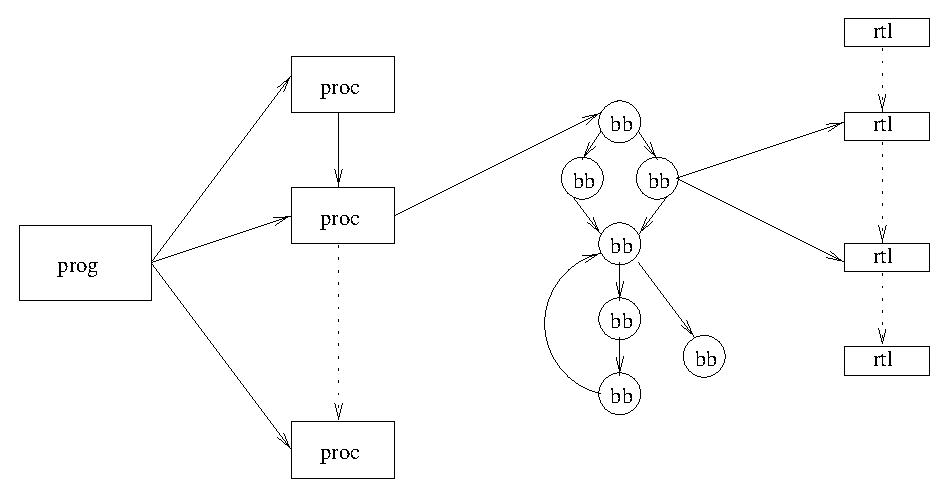
\includegraphics{figures/datastructs.eps}}
\centerfigend{fig-datastructs}{Data Structures to Represent a Binary Program}

We describe each of these parts of the intermediate representation
in reverse order, that is, starting from atomic data structures
and ending up with the program structure.



\section{Register Transfer Lists}
\label{sec-rtl}

{\small
\begin{flushright}
Design: Cristina, Mike; Documentation: Cristina, Doug, Mike;
 Implementation: Doug, David, Mike
\end{flushright} 
}

UQBT uses a simple, low-level register-transfer representation for the
effects of machine instructions.
A single instruction corresponds to a register-transfer list or RTL,
which in UQBT is a sequential composition of effects.
Each effect assigns an expression to a location.
All side effects are explicit at the top level;
expressions are evaluated without side effects, using purely
functional \emph{RTL operators}.
For example, the effects of the SPARC \texttt{call} instruction are
represented by the following RTL:

\begin{smallverbatim}
r[15] := %pc
%pc   := %npc
%npc  := r[15] + (4 * disp30)
\end{smallverbatim}
This sequence of effect puts the program counter~\texttt{\%pc} in
register~15, copies the ``next program counter''~\texttt{\%npc} into
the program counter, and puts the target address into~\texttt{\%npc}.
Because the target address is computed relative to the \emph{original}
program counter, the target-address computation uses register~15,
which holds the original value of~\texttt{\%pc}.
Because the SPARC uses delayed branches,  the target address
is placed into \texttt{\%npc}, not directly into \texttt{\%pc}.

Register transfer lists (RTLs) capture the semantic information 
of machine instructions by means of a series of \emph{effects} on a 
\emph{location}.
One register transfer is an assignment of an expression (i.e. an 
effect) to a location (i.e. a register or memory).  
There are no side effects, all effects are explicitly mentioned in 
the RTL.
The RTL environment assumes an infinite number of registers and
infinite memory space.  Memory is a sequence of bytes.  
{\it We will need specialized types of memory, such as memory for 
local variables, once the analysis has been formalized.   We
will do that then, so for now, there is only one type of memory. }

An `RTL language' is defined by a collection of locations and
operators.
UQBT uses an RTL language defined by taking the union of locations on
machines M$_S$ and M$_T$ and the union of the operators used in the
descriptions of machine M$_S$ and M$_T$.
The `machine~$X$ invariant' defines a sub-language of RTLs called
the $X$-RTLs; an RTL is an $X$-RTL if and only if it can be represented
as a single instruction on machine~$X$.

\uqbt 's \rtl\ implements the semantic information expressed in SSL
notation (SSL is described in Chapter~\ref{ch-ssl}).  

\subsection{Types}
\label{sec-rtltypes}
We define the following types to work with RTLs.  
(NOTE that these names should be in uppercase and perhaps shorter.
I've listed them as they appear in the rtl.h interface so that we don't
get confused -- when those are updated, these should be updated).
\begin{description}
\item[RTlist] a list of register transfers. Various analysis
    functions work on RTlists, such as GetControlTransfer().

\item[RTLInstDict] a dictionary of expanded instructions from the SSL
    file.

\item[RT] a register transfer is an assignment statement
    which has a variable (i.e. location) as the left-hand
    side and an expression (i.e. value) on the right-hand side. \\
    {\it We have considered introducing in the future a specialized
    RT which is a call, but at present that has not been decided
    upon.  We think it will be useful for analysis purposes. }

\item[RTAssgn] a subclass of class RT, representing an RT assignment
    (i.e. location := expression). One instruction may have zero
    (for NOP only) or more of these.

\item[RTFlagDef] a subclass of class RT, representing the definition
     of a flag function.

\item[RTFlagCall] a subclass of class RT, representing the call to a
    flag function.

\item[SemStr] a Semantic String, which is a prefix linearisation of an
    expression tree (see below).
    A SemStr can be used to represent a location, value, or subexpression.

    Expression operators are reproduced in Figure~\ref{fig-expOps2}.

% I'm not sure what this was meant to be about... probably some restriction
% on expressions which has long faded from the code. I keep it in comments
% in case it's not what I think it is. MVE
\begin{comment}
    {\it This may need to go elsewhere - Mike}
    An address expression is constrained to plus or minus offsets 
    from an address, hence the case \texttt{M[reg + reg * kte]} is not 
    supported directly; a subexpression needs to be computed into a 
    register and used as a register index in this case.

    These 3 options can be represented by 2: registers or constants.
    When an address expression is received, it is computed into 
    a register and that register is used to index into memory. 
    In this way we do not constrain address expressions (given that
    other machines may have more complicated addressing modes) 
    and create a simpler interface.
\end{comment}

\end{description}

\centerfigbegin
\begin{tabular}{|l|l|c|c|c|l|l|} \hline
Type of Operator & Id       &
\multicolumn{3}{c|}{Arguments}
& Symbol    & Meaning \\ \cline{3-5}
    &   & Int & Fix & Var & & \\
\hline
unary       & idNot         &0&0&1  & \verb!~!  & logical not \\
            & idNeg         &0&0&1  & 0-        & unary minus \\
\hline
binary      & idPlus        &0&0&2  & +         & addition \\
            & idMinus       &0&0&2  & -         & subtraction \\
            & idMult        &0&0&2  & *         & multiplication (unsigned)\\
            & idMults       &0&0&2  & *!        & multiplication (unsigned)\\
            & idDiv         &0&0&2  & /         & division (signed) \\
            & idDivs        &0&0&2  & /!        & division (signed) \\
            & idMod         &0&0&2  & \%        & modulus (unsigned) \\ 
            & idMods        &0&0&2  & \%!       & modulus (signed) \\ 
            & idBitAnd      &0&0&2  & \&        & (bitwise) and \\
%           & idBitAndNot   &0&0&2  & \&\~      & (bitwise) and-not \\
            & idBitOr       &0&0&2  & $|$       & (bitwise) or \\
%           & idOrNot       &0&0&2  & $|$\~     & (bitwise) or-not \\
            & idBitXor      &0&0&2  & \verb!^!  & xor \\
%           & idBitXorNot   &0&0&2  & \verb!^~! & xor-not \\
            & idShiftR      &0&0&2  & $>>$      & right-shift \\
            & idShiftL      &0&0&2  & $<<$      & left-shift \\
            & idShiftRA     &0&0&2  & $>>$A     & right-shift-arithmetic \\
            & idRotateL     &0&0&2  & rl        & rotate-left \\
            & idRotateR     &0&0&2  & rr        & rotate-right \\
            & idRotateLC    &0&0&2  & rlc       & rotate-left-through-carry \\
            & idRotateRC    &0&0&2  & rrc       & rotate-right-through-carry \\
\hline
ternary     & idTern        &0&0&3  & ?:        & c-style ternary \\
            & idAt          &0&0&3  & @         & bit extraction \\
\hline
logical     & idEquals      &0&0&2  & =         & equal \\
            & idNotEqual    &0&0&2  & \verb!~=! & not equal \\
            & idLess        &0&0&2  & $<$       & less than, signed \\
            & idGreater     &0&0&2  & $>$       & greater than, signed \\
            & idLessEq      &0&0&2  & $<=$      & less or equal to, signed \\
            & idGreaterEq   &0&0&2  & $>=$      & greater or equal to, signed \\
            & idLessUns     &0&0&2  & $<$u      & less than, unsigned \\
            & idGtrUns      &0&0&2  & $>$u      & greater than, unsigned \\
            & idLessEqUns   &0&0&2  & $<=$u     & less or equal to, unsigned \\
            & idGtrEqUns    &0&0&2  & $>=$u     & greater or equals, unsigned \\
            & idAnd         &0&0&2  & and       & and (of two expressions) \\
            & idOr          &0&0&2  & or        & or \\
\hline
operations  & idMemOf       &0&0&1  & m[...]    & memory of \\
            & idRegOf       &0&0&1  & r[...]    & register of \\
            & idAddrOf      &0&0&1  & a[...]    & address of (cancels m[]) \\
            & idVar         &1&0&0  & v\it{n}   & variable; replaces reg or mem \\
            & idParam       &0&1&0  & param`...'& parameter \\
            & idRparam      &0&1&0  & rparam`...'& register parameter \\
            & idExpand      &0&1&0  & expand`...'& expand (not for user) \\
            & idTemp        &0&1&0  & temp`...' & temporary register \\
            & idSize        &1&0&1  & size \it{n}& size cast \\
            & idDef         &0&1&0  & def `...' & definition; special for UQDBT \\
            & idIndex       &0&0&2  & [...]     & special for UQDBT \\
\hline
constants   & idIntConst    &1&0&0  & int \it{n}& integer constant \\
            & idFloatConst  &2&0&0  & float \it{f}& floating point constant \\
\hline
\end{tabular}
\centerfigend{fig-expOps2}{Expression Operators for RTL (cont over page)}

\centerfigbegin
\begin{tabular}{|l|l|c|c|c|l|l|} \hline
Type of Operator & Id       &
\multicolumn{3}{c|}{Arguments}
& Symbol    & Meaning \\ \cline{3-5}
    &   & Int & Fix & Var & & \\
\hline
type conversions& idSignExt &0&0&1  & !         & sign-extend (no sizes) \\
            & idTrunc       &2&0&1  & trunc(\it{exp, s1, s2})& truncate from s1 to s2 bits \\
            & idZfill       &2&0&1  & zfill(\it{exp, s1, s2})& zero fill from s1 to s2 bits \\
            & idSgnEx       &2&0&1  & sgnex(\it{exp, s1, s2})& sign extend from s1 to s2 bits \\
\hline
float conversions&idFsize   &2&0&1  & fsize(\it{exp, s1, s2})& float size convert from s1 to s2 \\
            & idItof        &2&0&1  & itof(\it{exp, s1, s2})& integer to float, s1 to s2 bits \\
            & idFtoi        &2&0&1  & ftoi(\it{exp, s1, s2})& float to integer, s1 to s2 bits \\
            & idFround      &2&0&1  & fround(\it{exp, s1, s2})& float round, s1 to s2 bits \\
\hline
\end{tabular}
\centerfigend{fig-expOps2a}{Expression Operators for RTL (cont from prev page)}

\subsection{Interface Functions to Create and Use RTLs}
All objects have constructor and destructor functions, as well
as functions to access elements of an object.  
Specialized analysis-related functions are explained in the
last subsection of this section---Functions for Analysis 
Purposes.  \\
{\it This style file doesn't number subsub sections,
how annoying! }


\subsubsection{Semantic String Class}
A semantic string object (SemStr) is a prefix linearisation of a tree
of RT components, such as constants, registers, memory, and various
expressions involving these. It is inplemented as a list of integers
(called items);
many of these integers are indices into a special table called the
Semantic Table. Entries in this table represent various things, such
as operators, special registers, parameters, and so on.

Here are a few examples: index 0 (the first entry) is called \texttt{idPlus},
and represents binary addition. Approximately index 75 is called
\texttt{idIntConst}, representing an integer (the actual integer is the next
integer in the string, following the {\tt idIntConst}).  So the expression
\texttt{2+2} is represented by the string ``{\tt 0 75 2 75 2}'' (read this
as ``plus int 2 int 2''). 

All the operators listed in Figure~\ref{fig-expOps2} are automatically
included in the table, and they are
machine independent. Special registers (e.g. the Next Program Counter register
({\tt \%npc}) and parameters (e.g. {\tt rs1} for the first source
register) are added
by the parser of the SSL file (see Chapter~\ref{ch-ssl}).
Let's consider a complete RTAssgn, conventionally written as

{\tt r[4] = m[1000] + 5}

This will be implemented as two semantic strings, one for the
location (left hand side) and one for the value (right hand side).
Each will be a list of integers, which might be

{\tt 34 75 4} ~~~and~~~ {\tt 0 38 75 1000 75 5}

and might print as

{\tt r[4]} ~~~and~~~   {\tt m[1000] + 5}  ~~~normally (the "int" is dropped
for brevity), or

{\tt r[ int 4]}  ~~~and~~~  {\tt + m[ int 1000 ] int 5}

if you choose to use the printPrefix() member function. This latter
representation is better for debugging problems with semantic strings,
though obviously it is less readable.

The first SemStr could be read as ``RegOf int 4''. The first integer, 34,
is an index into the semantic table, where among other information
there is the string ``r['' (for the SemStr print routine).
The enumerated constant ``idRegOf'' can be used in programs to
represent this index (see Figure~\ref{fig-expOps2} for a complete list
of these enumerated constants). The second integer,
75, is also an index into the semantic table, and says that the integer
following this index is to be taken as a literal integer. The third
integer, 4, represents itself. The second semantic string is a little
more complex. Its first index, 0, represents addition. The two arguments
to be added come next, but they are variable length. Immediately after
the 0 is 38, representing "memory of". The thing following the MemOf
could be any kind of expression; in this case it's ``int 1000'', but
it could have been say ``{\tt+ 500 500}'', or ``{\tt - r[ int 16 int 8}''.

Note that special registers (such as {\tt \%pc} or {\tt \%CF}) are
represented differently from general purpose registers. General purpose
registers are numbered, whereas special registers have their own
index into the semantic table (see Section~\ref{sec-semtable}).

A word on nomenclature: the word {\it parameter} is used to describe
a part of an instruction that will be {\it instantiated} with the
RTL function. For example, ``regorimm'' could be a parameter representing
a part of an instruction; actual values could be ``r[4]'' or ``4''.
The word {\it argument} is used here to mean those parts of a semantic
string that represent arguments (or operands) to the first index. For example,
if the first index is {\tt idMinus}, then there are two variable length
arguments to it, representing the minuend and the subtrahend respectively.
If the first index is idSize, there is one integer argument (the number
of bits in the size being cast to), and one variable length argument
(the expression being size cast).

Every semantic string has a type (e.g. unsigned integer 32 bits); the type is
represented by class Type (see Section~\ref{sec-class-type}). If not explicitly
specified, the semantic string is assigned the default type (which is signed
integer 32 bits). This type is preserved when semantic strings are copied,
subexpressions are made, and so on.

\begin{itemize}
\item   SemStr: $\emptyset$ \ra SemStr.
    Default constructor.

\item   SemStr: Kind \ra SemStr.
    Constructor that takes an expression kind. The kinds are only these:
    uORDINARY, eOPTABLE, and eCONDTABLE. Not for users.

\item   SemStr: SemStr \ra SemStr.
    Copy constructor.

\item   operator=: SemStr \ra SemStr.
    Assignment operator.

\item   SemStr: (Iterator1 x Iterator2) \ra SemStr.
    Constructor that takes a pair of iterators. Makes a copy of part
    of some other SemStr starting with the item referenced by iterator1
    up to but not including iterator2.

\item   SemStr: (int* x int* x Kind) \ra SemStr.
    Constructor that takes two pointers to an array of integers (pointer to
    first and pointer to last). Also takes kind, as above.

\item   getKind: SemStr \ra Kind.
    Gets the kind as above. Not for users.

\item   getType: SemStr \ra Type.
    Gets the type (as class Type) for the semantic string.

\item   isFloat: SemStr \ra BOOL.
    Note: deprecated. Returns true if the expression this semantic string
    represents is a floating point type.

\item   setType: (SemStr x Type) \ra $\emptyset$.
    Set the type for the expression that this semantic string represents.

\item   setTypes: (SemStr x SemStr) \ra $\emptyset$.
    Set the type for this semantic string to be the same as the type of the
    given semantic string.

\item   operator==: (SemStr x SemStr) \ra BOOL.
    Returns true if this SemStr is equal to the given SemStr. Type is taken
    into account in the comparison.

\item   operator\%=: (SemStr x SemStr) \ra BOOL.
    Same as above, except that type is \emph{not} taken into account.

\item   operator-=: (SemStr x SemStr) \ra BOOL.
    Same as the two above, except that only the sign element of the type is
    disregarded. Therefore, to return true, the expressions must match, and
    the size and broad type must match, but the ``signedness'' need not
    match.

\item   operator$<$: (SemStr x SemStr) \ra BOOL.
    Returns true if this SemStr is ``less than'' the given SemStr. Comparison
    is arbitrary, but establises a unique ordering of semantic strings. This
    function is often used implictly where there are maps of semantic strings.
    Type is included in the comparison.

\item   operator$<<$: (SemStr x SemStr) \ra BOOL
    Same as the above, except that ``signedness'' is not considered in the
    comparison.

\item   push: (SemStr x int) \ra $\emptyset$.
    Push the given integer to the end of the semantic string. It is up to
    the user to make sure that the semantic string is valid.

\item   prep: (SemStr x int) \ra $\emptyset$.
    Prepend the given integer to the front of the semantic string. It is
    up to the user to make sure that the semantic string is valid.

\item   pushSS: (SemStr x SemStr) \ra $\emptyset$.
    Push a copy of the given semantic string to the end of this string

\item   pushArr: (SemStr x int x int*) \ra $\emptyset$.
    Push the given number of integers from the given array of integers to
    the end of the string.

\item   pop: $\emptyset$ \ra int.
    Remove the last integer from the list, and return it.

\item   popFirst: $\emptyset$ \ra int.
    Remove the first integer from the list, and return it.

\item   clear: $\emptyset$ \ra $\emptyset$.
    Set this semantic string to be empty (no elements in the list).

\item   isSpRegEqual: (SemStr x int) \ra BOOL.
    Returns true if this semantic string matches the special register
    whose index is given. Not for most users.

\item   isSpRegCont: (SemStr x int) \ra BOOL.
    Returns true if this semantic string contains the special register
    whose index is given. Not for most users.

\item   isNumRegEqual: (SemStr x int) \ra BOOL.
    Returns true if this semantic string matches the register
    whose number is given. Not for most users.

\item   isNumRegCont: (SemStr x int) \ra BOOL.
    Returns true if this semantic string contains the register
    whose number is given. Not for most users.

\item   isArrayEqual: (SemStr x Array of int) \ra BOOL.
    Returns true if the elements of this semantic string match the
    elements of the given array of integers. Can be used to test for
    specific semantic strings, e.g. ``\%pc = \%npc''.

\item   getFirstIdx: SemStr \ra int.
    Returns the first item of this semantic string. Note that this really
    should be called getFirstItem, since the integer returned may not actually
    be an index (it could be an integer constant, or even half of a floating
    point constant).

\item   getSecondIdx: SemStr \ra int.
    Returns the second item of this semantic string. Usually used where
    the first index is known to contain one integer or fixed argument
    (e.g. the first index is idIntConst or idSize).

\item   getThirdIdx: SemStr \ra int.
    Returns the third item of this semantic string.

\item   getSubExpr: (SemStr x int) \ra SemStr*.
    Returns a pointer to a new semantic string, which is composed of
    the given subexpression. Passing zero returns the first argument
    to this expression, one returns the second, and so on.
    {\bf Note:} This member function only works with variable arguments.
    Use GetSecondIdx to access an integer or fixed argument.

\item   getSubExpr: (SemStr x int x SemStr) \ra SemStr.
    As above, but also stores the result in the reference (last) parameter.
    This ensures that the caller will automatically delete the semantic string
    when it goes out of scope.

\item   getIndex: (SemStr x int) \ra int.
    Get the {\it i}th item (where {\it i} is given).

\item   getLastIndex: SemStr \ra int.
    Get the last item of the list of integers in this semantic string.

    The next group of member functions concern searching for a subexpression
    withing this semantic string. An item of -1 in a semantic string is treated
    as a ``wildcard''.
    Formally, a search expression (S) will match a subexpression (E) if:

    length(S) $<=$ length(E) and for each position, p, in S the following holds:

    S[p] == -1 $||$ S[p] == E[p]

    Example: if {\it this} is \{0,\{3,78\},\{43,6,14\}\},
    it can be searched with the following subexpressions, and will return true:

\begin{tabular}{|l|l|} \hline
    Search & Result \\
\hline
    \{\{3,78\}\} & \{\{3,78\}\} \\
    \{\{0,*,*,\{43\}\}\} & \tt\{\{0,\{3,78\},\{43,6,14\}\}\} \\
\hline
\end{tabular}

\item   search: (SemStr x SemStr x SemStr x BOOL) \ra BOOL.
    Searches this semantic string for the given subexpression (first parameter
    after {\it this}). If found, the matching string is copied to the reference
    (last SemStr) parameter. The return value is whether a match was found.
    If the optional boolean is set, the search is type
    sensitive (i.e. the types have to match, as well as the expressions). This
    boolean defaults to false (i.e. the search defaults to case insensitive).

\item   searchAll: (SemStr x SemStr x list\{SemStr*\} x BOOL) \ra BOOL.
    Searches this semantic string for {\it all} occurrences of the given
    subexpression (first parameter after {\it this}). For each match, the
    matching string is appended to the list of pointers to semantic strings.
    The return value is whether any match was found.
    If the optional boolean is set, the search is type
    sensitive (i.e. the types have to match, as well as the expressions). This
    boolean defaults to false (i.e. the search defaults to case insensitive).

\item   searchReplace: (SemStr x SemStr x SemStr x BOOL) \ra BOOL.
    Searches this semantic string for the given subexpression (first parameter
    after {\it this}). If found, the matching string is replaced by the
    reference (last SemStr) parameter. The return value is whether a match was
    found.
    If the optional boolean is set, the search is type
    sensitive (i.e. the types have to match, as well as the expressions). This
    boolean defaults to false (i.e. the search defaults to case insensitive).

\item   searchReplaceAll: (SemStr x SemStr x SemStr x BOOL) \ra BOOL.
    Searches this semantic string for {\it all} occurrences of the given
    subexpression (first parameter after {\it this}). For each match, the
    matching string is replaced by the given string (last SemStr parameter).
    The return value is whether any replacement was made.
    If the optional boolean is set, the search is type
    sensitive (i.e. the types have to match, as well as the expressions). This
    boolean defaults to false (i.e. the search defaults to case insensitive).

\item   substReg: (SemStr x int x SemStr) \ra BOOL.
    Substitute all occurrences of the given numbered register with the given
    semantic string. Returns true if any match found.
 
\item   substSpcl: (SemStr x int x SemStr) \ra BOOL.
    Substitute all occurrences of the given special register (index is given)
    with the given semantic string.

\item   substIndex: (SemStr x int x int) \ra $\emptyset$
    Replace the item at the given index with the given integer. For example,
    substIndex(0, 77) will replace the first item in the list with 77.
 
\item   smartCompare: (SemStr x SemStr x BOOL x list\{int\}) \ra BOOL.
    This function is not complete. Do not use.

\item   findEndSubExpr(SemStr x iterator) \ra iterator.
    Given an iterator into this semantic string, step forward towards the end
    of this string until the end of the subexpression headed by the given
    iterator is found. Returns an iterator that is just past the end of that
    subexpression. For example, if given (3+4)*(5+6) (internally
    * + int 3 int 4 + int 5 int 6), with an iterator pointing to the first
    plus, returns an iterator to the second plus (just past the (3+4)
    subexpression).
    There are actually two functions with the same name; one takes and
    returns a const iterator, and one takes and returns a non-const iterator.

\item   simplify: SemStr \ra $\emptyset$
    Simplify this expression using constant folding and the like, and also
    cannonicalising the expression by placing integer constants on the
    right if possible (so 2+a is replaced by a+2). a + -2 is replaced by a-2.
    a $<<$ k is changed to a * K where K=2**k.

\item   findSubExpr: (SemStr x int x int* x int) \ra BOOL.
    Search this semantic string for the expression (given by the given number
    of integers in the given array of integers). Returns true if found. If
    found and there were wildcards in the array, the item matched by the last
    wildcard is written to the reference (last) parameter.

\item   sprint: SemStr \ra string.
    Prints a representation of this semantic string to a string, which
    is returned. This is a conventional (infix) representation, and
    so it somewhat removed from the actual (prefix) implementation.
    Some effort is made to pretty the result, e.g. r[ int 4] is
    displayed as r[4].
    When exact knowledge of the format of the string is required, use
    sprintPrefix below.

\item   print: (SemStr x ostream) \ra $\emptyset$.
    Prints a representation of the semantic string to the given stream,
    or to cout if none is given. It is equivalent to printing the string
    returned by sprint to the given stream.

\item   sprintPrefix: SemStr \ra string.
    Prints a representation of this semantic string to a string, which
    is returned. The format is strongly tied to the internal (prefix)
    representation of the semantic string, so it is harder to read than
    the result from sprint, but may be more useful for debugging.

\item   printPrefix: (SemStr x ostream) \ra $\emptyset$.
    Prints a representation of the semantic string to the given stream,
    or to cout if none is given. It is equivalent to printing the string
    returned by sprintPrefix to the given stream.

\item   len: SemStr \ra int.
    Returns the number of items in this semantic string.

\item   instantiate: (SemStr x list\{int\} x vector\{char*\} x RMAP) \ra BOOL.
    Replace all occurrences of formal instruction parameters (e.g. rs1) with
    actual expressions (e.g. r[12]). The last parameter is an object
    representing the register map. Not for users.

\end {itemize}

\subsubsection{Semantic Table Class}
\label{sec-semtable}

Semantic Strings (class SemStr) are mainly indices into a special
object of class SemTable, the semantic table. This is a global
object, accessable as {\tt theSemTable} as long as you
{\tt \#include "ss.h"}. Most of the time, the user need not be
concerned with the semantic table, but there are a few important
exceptions.

One of these is when dealing with special registers. These registers
are not accessed like general purpose registers (so called {\it numbered}
registers), but have their own entries in the semantic table. When
special registers are referenced in the SSL file (see Chapter~\ref{ch-ssl}),
they are placed into
the semantic table by the parser. The index of a particular special
register is not fixed (most of them are machine specific), so there is no
enumerated constant like {\tt idPlus} that can be used for a special
register. At present, the way to find an appropriate index is to use
the FindRegIndex member function.

\begin{itemize}
\item   findRegIndex: (SemTable x string) \ra int.
    Given the semantic table and a string representing the name of the
    special register (including the {\tt \%}), returns an integer index
    for the appropriate semantic table item. This single index
    represents the special register in semantic strings (compared with
    three integers for a numbered register).

\item   findOpIndex: (SemTable x char*) \ra int.
    Given a C string representing the operator (e.g. {\tt \verb!"&~"!}),
    returns the index representing the operator. This operator can be
    used to build expressions, etc. Note that this function is not
    efficient (at present, it uses a linear search), so it should not
    be used where the operator is known (in this case, {\tt idBitAndNot});
    use it where the operator could be one of a number of values, and
    only the string representation is known. (For example, the SSL
    parser uses this function when parsing SSL expressions).

\end{itemize}

\subsubsection{Type Class}
\label{sec-class-type}
Types inside Semantic Strings and elsewhere are represented by class Type.
A Type has three components: the broad type, sign, and size. The broad type
is given in terms of this enumerated type:

\begin{verbatim}
enum LOC_TYPE {
    VOID = 0,               // void (for return type only)
    INTEGER,                // integer (any size and signedness)
    FLOAT,                  // a floating point (any size)
    DATA_ADDRESS,           // a pointer to some data (e.g. char*, struct*,
                            // float* etc)
    FUNC_ADDRESS,           // a pointer to a function
    VARARGS,                // variable arguments from here on, i.e. "..."
    UNKNOWN
};
\end{verbatim}

A particular type is given by either a tuple (e.g. (INTEGER, unsigned, 32 bits))
or a couple (e.g. (FLOAT, 64 bits); the sign is irrelevant for a float, but
defaults to signed).

\begin{itemize}
\item   Type: $\emptyset$ \ra Type.
    Default constructor. Returns the default type, which is 32 bit signed
    integer.

\item   Type: (LOC\_TYPE x int x BOOL) \ra Type.
    Constructor, with type given as a LOC\_TYPE (see abvove), size in bits,
    and if the LOC\_TYPE is integer, a BOOL for sign (TRUE = signed).

\item   operator==: (Type x Type) \ra BOOL.
    Equality operator. Sign is considered in the comparison, so the types must
    match in all respects for this function to return TRUE.

\item   operator-=: (Type x Type) \ra BOOL.
    Equality operator. Sign is {\it not} considered, so for this function to
    return true, the broad types and size must match, but the sign need not.

\item   operator$<$: (Type x Type) \ra BOOL.
    Less than operator. Sign is considered in the comparison.
    This function establishes an arbitrary ordering among all types.

\item   operator$<<$: (Type x Type) \ra BOOL.
    Less than operator. Sign is {\it not} considered in the comparison.
    This function establishes an arbitrary ordering among all types.

\item   getSize: Type \ra int.
    Returns the size (in bits) component of the Type.

\item   getType: Type \ra LOC\_TYPE.
    Returns the Type component of the Type, as a LOC\_TYPE.

\item   getSize: Type \ra BOOL.
    Returns the sign component of the Type; TRUE if signed.

\item   setSize: (Type x int) \ra $\emptyset$.
    Sets the size (in bits) component of this Type.

\item   setType: (Type x LOC\_TYPE) \ra $\emptyset$.
    Sets the Type component of this Type, given a LOC\_TYPE.

\item   setSize: (Type x BOOL) \ra $\emptyset$.
    Sets the sign component of this Type; TRUE if signed.

\item   getCtype: Type \ra CHAR*.
    Returns a C-style null terminated string representing the C language
    equivalent of the type. For example, if the type is (integer, unsigned, 16)
    the returned string would be ``unsigned short''.

\end{itemize}


\subsubsection{Register Transfer Assignment Class}
A register transfer assignment (RTAssgn) object is an assignment of an
expression
to a location.  A register transfer object also has size information
to determine the number of bits of information transferred from
the expression to the location.

\begin{itemize}
\item  updateLHS: (RTAssgn x Location) \ra RT.
    Given an RT object and a location, the location
    information gets updated in the object.

\item  updateRHS: (RTAssgn x Expr) \ra RT.
    Given an RT object and an expression, the expression
    information gets updated in the object.

\item  updateSize: (RTAssgn x BYTE) \ra RT.
    Given an RT object and a size in bits, the size of the
    transfer information gets updated in the object.

\item  getLHS: RTAssgn \ra SemStr*.
    Given an RTAssgn object, returns a pointer to the semantic string
    representing the location of the assignment.

\item  getRHS: RTAssgn \ra SemStr*.
    Given an RTAssgn object, returns a pointer to the semantic string
    representing the expression of the assignment.

\item  getSize: RTAssgn \ra BYTE.
    Given an RT object, returns the size in bits of the transfer
    of information.
\end{itemize}


\subsubsection{Register Transfer List Object}
A register transfer list (RTlist) is a list of register transfer 
objects.  However, greater functionality is provided for this 
object for analysis purposes; those functions are described in the 
next section.
For traversal purposes, an RTlist keeps track of the `current'
register transfer being traversed (by default, the first one
in the list).

\begin{itemize}
\item RTlist: $\emptyset$ \ra RTlist.
    Constructor function which returns an empty object of type RTlist.

\item RTlist: (RTlist x RTlist) \ra RTlist.
    Copy constructor: given a source and destination RTlist 
    objects, copies the first one onto the second one.

\item insertRT: (RTlist x RT) \ra RTlist.
    Given an RTlist object and a register transfer, inserts the
    register transfer at the end of the list.

\item updateRT: (RTlist x RT x int) \ra RTlist.
    Given an RTlist object, a register transfer and an index position into
    a list, updates the indexed register transfer in the list
    with the new one (if possible), otherwise it does not modify
    the RTlist object.
\end{itemize}


\subsubsection{Functions for Analysis Purposes}
The following functions are required for analysis purposes and
are described per relevant object.
More functions will be added as we see fit.


\paragraph{Register Transfer Assignment Class}
Functions that allow users to know which registers are defined
and used in the register transfer.  Note that this information
is implicitly stored in the LHS and RHS fields of an 
RTAssgn object.

\begin{itemize}
\item  isSpRegDefined: (RTAssgn x int) \ra BOOL.
    Given a register transfer assignment object and an index representing
    a special register, returns 
    whether the register is defined in the assignment or not.

\item  isNumRegDefined: (RTAssgn x int) \ra BOOL.
    Given a register transfer assignment object and the number of a
    numbered register, returns whether that register was defined
    in the register transfer or not.

\item  isSpRegUsed: (RTAssgn x int) \ra BOOL.
    Given a register transfer assignment object and an index representing
    a special register, returns whether
    that register was used by the object or not.

\item  isNumRegUsed: (RTAssgn x int) \ra BOOL.
    Similar to IsRegUsed() but for a numbered register.

\item  numRegUse: RTAssgn \ra int.
    Given a register transfer object, returns the number of registers
    used by that transfer. \\
    {\it Not implemented at present. A similar function that returns a list of registers used may
    be useful. }

\item  numRegDef: RTAssgn \ra int.
    Given a register transfer object, returns the number of registers
    that were defined by that transfer. \\
    {\it Not implemented at present. A similar function that returns a list of registers defined may
    be useful. }
\end{itemize}


\paragraph{Register Transfer List Object} 
The RTlist object \emph{will} provide in the \emph{future} 
functions that allow us to quickly decide what type of 
instructions we are dealing with.  The following are two
such functions which are not currently implemented:

\begin{itemize}
\item RTL: (STRING x ADDRESS x ...) \ra RTlist.
    This function returns an instance of a register transfer
    list for a particular machine instruction.  The name
    of the instruction is a named used in the SSL specification,
    these names are normally the same names used in SLED
    specifications.   The given native address is the program counter's
    address and is stored for usage when building a control
    flow graph of the procedure (see Section~\ref{sec-cfg}). \\ 
    The function returns an instance of an RTlist by reading
    the template file generated by SRD (refer to Section~\ref{sec-srd},
    Chapter~\ref{ch-ssl}).  \\

\item getBBSuccAddr: (RTlist x int) \ra ADDRESS.
    Given an RTlist object and an index position, returns the 
    address associated with that out-edge (if any) or Nil 
    otherwise.  \\
    This function is useful to construct a control flow graph,
    see example in Section~\ref{sec-cfg-eg}. 

\item getBBProcAddr: RTlist \ra ADDRESS.
    Given a call register transfer list, returns the target procedure 
    call address (if any) or Nil otherwise. \\
    This function is useful to construct a control flow graph,
    see example in Section~\ref{sec-cfg-eg}.

\item getNumRT: RTlist \ra int.
    Given an RTlist, returns the number of elements (RTs) in
    the list.

\item getRT: (RTlist x int) \ra RT.
    Given an RTlist object and an index into the list, returns
    the corresponding register transfer (if it exists) or 
    Nil.
    Elements in a list are indexed from one.

\item nextRT: RTlist \ra RT.
    Given an RTlist object, returns the next RT in the list (if any)
    or Nil (if at the end of the list).  The `current' index is
    updated to point to the next element in the list. 

\item isControlTransfer: RTlist \ra CTTYPE.
    Given an RTlist object, checks if the set of register 
    transfers are equivalent to a control transfer instruction,
    if so, returns the type of control transfer instruction 
    (one of ONEWAY, TWOWAY, NWAY, CALL, or FALL), otherwise
    returns NONE.  
    A control transfer instruction is one that explicitly 
    modifies the value of the program counter register.
\end{itemize}



\subsection{Usage of this Interface}
\label{sec-usageRTL}
A user can integrate RTL into a NJMC matching statement in
the following way: once an instruction has been decoded 
by matching one of the arms of the \texttt{match} statement, 
an instance of the matched instruction can be obtained in 
RTL form by passing the (unique) name of the instruction to
the RTL dictionary, along with the values of the other parts
of the instruction.  The RTL system will return an instance
of an entry in the dictionary. 
At present, the RTL instance function expects to receive 
the native address of the instruction being decoded, its name 
(i.e. key), and its arguments in string form.  The native 
address is required later on, for the purposes of constructing
a control flow graph of the program (see Section~\ref{sec-cfg}).

The following sample code illustrates the usage of this interface
with a SPARC matching statement.
The function \texttt{decode\_instr} implements a matching statement
which decodes the machine instruction pointed to by the \texttt{pc}
variable.  If the \texttt{alu} arm is matched, the \texttt{name} 
variable will hold the name of the arithmetic-logical instruction
matched.  The \texttt{RTLDisc.RTL} function is called with the
string values for the other parts of the arithmetic-logical 
instruction: the first register operand (\texttt{rs1}), the 
second register or immediate operand (matched in the \texttt{dis\_roi}
function), and the destination register \texttt{rd}).  Macros
are used (\texttt{RS1}, \texttt{ROI} and \texttt{RD}) to make
the translation from integer to strings depending on the context.
In the case of branch and call instructions, the target address passed
to the RTL dictionary is the \emph{raw} offset address given in the
instruction, rather than the relocated one; hence the need for the
equation provided to restore this value.  Alternatively, the 
core SLED spec for SPARC could be modified so that it does not 
relocate addresses automatically---this has not been done at 
present for consistency with disassemblers.

{\small
\begin{verbatim}
#define RD   (rd_names[rd])
#define RS1  (rs1_names[rs1])
#define RS2  (rs2_names[rs2])
#define ROI  (dis_roi(roi))

char *dis_roi(ADDRESS lc) {
  static char buf[512];
  match lc to
  | imode(i)   => sprintf(buf, "%d", i); return buf;
  | rmode(rs2) => return RS2;
  endmatch
}

void decode_instr (ADDRESS pc, ADDRESS uNativeAddr, RTLInstDict RTLDict, RTlist &rtl)
{
    match pc to
    | ...
    | alu (rs1, roi, rd) [name] => 
            rtl = RTLDict.RTL (uNativeAddr, name, RS1, ROI, RD);
    | branch^a (tgt, a) [name] => 
            sprintf(anulled, "%d", a);      // 1 if anulled
            rtl = RTLDict.RTL (uNativeAddr, name, numToStr((tgt-pc)>>2), anulled);
    | call_ (tgt) [name] => 
            rtl = RTLDict.RTL (uNativeAddr, name, numToStr((tgt-pc)>>2)); 
    | ...
    endmatch
\end{verbatim}  
}

This type of code (the whole matching statement file) can
obviously be mostly generated automatically, but at this stage we
either generate a decoder usingthe NJMC toolkit and modify that
code, or write it manually.


\section{Control Flow Graphs}
\label{sec-cfg}

{\small
\begin{flushright}
Design: Cristina; Documentation: Cristina; Implementation: Mike, Cristina
\end{flushright} 
}

A control flow graph (CFG) is a directed graph that represents the flow of 
control of a program, thus, it only represents the flow of instructions 
(code) of the program and excludes data information.
The nodes of a CFG represent basic blocks of the program, and the edges 
represent the flow of control between nodes.  More formally,

\begin{definition} \cite{Aho86}
\label{def-bb}
A {\bf basic block} is a sequence of consecutive statements in which
flow of control enters at the beginning and leaves at the end without
halt or possibility of branching except at the end.   
\end{definition}


\begin{definition}
\label{def-cfg}
A {\bf control flow graph} $G = (N,E,h)$ for a program $P$ is a connected,
directed graph, that satisfies the following conditions:
\begin{itemize}
\item $h$ is the unique entry node to the graph, 
\item $\forall \, n \in N, n$ represents a basic blocks of $P$, and 
\item $\forall \, e = (n_{i},n_{j}) \in E, e$ represents flow of control from
basic block $n_{i}$ to basic block $n_{j}$, and $n_{i}, n_{j} \in N$.
\end{itemize}
\end{definition}


\subsection{Types of Basic Blocks}
For the purposes of CFG construction, basic blocks are
classified into different types, according to the {\em last} instruction in 
the basic block.  Given that the instructions in the basic block
represent a sequential list of instructions (that would be executed
in that order), machine dependencies on the flow of control such as 
SPARC's delayed instructions cannot appear in the graph; they need
to be abstracted away into a machine-independent form.

Ideally, only 6 types of basic blocks are available.  However, 
during static decoding of a binary executable, it is not always
possible to determine the target branches of indirect and indexed
transfers of control.  In these cases, we make use of a node called
{\em nowhere} as the node does not lead to anywhere.  This node
will be analysed at runtime.  
The basic block types are: 

\begin{description}
\item [one-way] the last instruction in the basic block is an
unconditional jump to a known target location, hence, the block has one 
out-edge.

\item [two-way] the last instruction is a conditional jump to a 
known target location, thus, the block has two out-edges.

\item [n-way] the last instruction is an indexed/indirect jump to
known target locations.  The $n$ branches located in the index table become 
the $n$ out-edges of this node.

\item [call] the last instruction is a call to a procedure.
There are two out-edges from this block: one to the instruction following
the procedure call, and the other to the procedure that is called.
Throughout analyses, the called procedure is normally not followed,
unless interprocedural analysis is required.

\item [return] the last instruction is a procedure return instruction.
There are no out-edges from this basic block.

\item [fall] the next instruction is the target address of a
branch instruction (i.e. the next instruction has a label).  This node
is seen as a node that {\it falls through} the next one, thus, there is
only one out-edge.

\item [nowhere] the last instruction is an indexed or indirect jump
or call to an unknown target location.  This node has no out-edges. 
\end{description}


\subsection{Abstractions}
Based on definitions~\ref{def-bb} and \ref{def-cfg}, we define two 
abstractions to work with control flow graphs.

\begin{description}
\item [BB] is a basic block.  A BB holds information about the
    RTL instructions that form part of that basic block, as 
    well as successors of the basic block.

\item [CFG] is a control flow graph.  A CFG is a reference to 
    the header of the graph, i.e. a BB, and stores extra information
    like the state of the graph (see next section).
    Extra functionality is provided for a CFG which is not 
    provided for a BB, as seen in Section~\ref{sec-ir-cfg}.
\end{description}


\subsection{Steps in Constructing a CFG}
Machine instructions that modify the flow of control of a program 
have two types of references to the target address: via a machine-dependent
(physical) address, or via an offset into the stream of machine
instructions for the program.  Offsets resolve to physical 
addresses too.   
There are three main steps in the construction of the CFG:
\begin{enumerate}
\item Create a machine-dependent CFG by building BBs of instructions
    that contain native addressess for transfers of control.
\item Transform the machine-dependent CFG into a machine-independent
    CFG by transforming address references into edges (references
    to basic blocks).
\item Optimize the machine-independent CFG to remove extraneous 
    basic blocks introduced by limitations in the machine 
    instruction set (e.g. a jump to a jump), hence reducing the 
    number of nodes and edges of the graph. 
\end{enumerate} 

We will refer to the machine-independent CFG as a {\em well-formed} CFG
or \wfCFG.  This graph is the one used for analysis purposes. 


\subsection{Interface Functions to Construct Basic Blocks}
\label{sec-ir-bb}
Basic blocks have limited functionality: they can be 
constructed, and machine-dependent (i.e. host address) out-edges 
can be added to them. 

\begin{itemize}
\item BasicBlock: $\emptyset$ \ra BB.
    Constructor for a basic block.

\item addOutEdge: (BB x ADDRESS) \ra BOOL.  
    Adds the address as an out-edge in the given basic block. 
    The mapping between addresses and basic blocks is done when 
    the graph is well-formed.
    Returns true if successful.

\item addInterProcOutEdge (BB x ADDRESS) \ra BOOL.
    Adds an interprocedural out-edge to the basic block pBB that
    represents this address.  The mapping between addresses and
    basic blocks is done when the graph is well-formed.
    Returns true if successful.

\item addProcOutEdge: (BB x ADDRESS) \ra BOOL.
    Given a CALL basic block and an address of a procedure (i.e. the
    target address of a call instruction), stores the information
    in the basic block. 
    \emph{This function is not yet implemented.}
\end{itemize}


\subsection{Interface Functions to Construct a CFG}
\label{sec-ir-cfg}
Control flow graphs are composed of machine-dependent basic block nodes 
initially, and can then be transformed to machine-independent nodes
which are used for analysis purposes.  This latter graph is referred
to as a well-formed graph. 
A doubly-linked graph (i.e one that has in- and out-edges) can only be 
built once the graph is well-formed.
Further, a well-formed graph can be optimized to remove redundant edges 
and nodes (e.g. jumps to jumps).
The following functionality is provided by the interface:

\begin{itemize}
\item Cfg: $\emptyset$ \ra Cfg.
    Constructor function for a CFG. The CFG is constructed empty, and
    has BBs added as required.

\item newBB: (CFG x RTL x RTL x BBTYPE x int x ADDRESS) \ra BB.  
    Allocates memory for a new basic block node, initializes it to 
    references to the first and last rtl's, its type, and allocates 
    enough space to hold the out-edges (the number of which is 
    given as a parameter).  
    The native address associated with the start of the BB is given;
    this address must be the same one used with AddOutEdge().
    A reference to the newly created basic block is returned.
    If there is not enough memory, an exception will be raised.
    \emph{Mike: what did we decide in the end for these cases?}

\item label: (CFG x ADDRESS) \ra BOOL.
    Checks whether the given native address is a label (explicit or 
    non-explicit) or not.  Explicit labels are addresses that have already 
    been tagged as being labels due to transfers of control to that 
    address.  Non explicit labels are those that belong to basic blocks 
    that have already been constructed (i.e. have previously been 
    parsed) and now need to be made explicit labels.  In the case of 
    non explicit labels, the basic block is split into two and types 
    and edges are adjusted accordingly.
    Returns true if the native address is that of an explicit or a non 
    explicit label, false otherwise. 

\item isLabel: (CFG x ADDRESS) \ra BOOL.
    Checks if the native address is a label or not in the current 
    control flow graph. 
    If not, the address is not added to the map of Lables to BBs.
    \emph{Mike: what does the last sentence mean?  i.e. every time
    an IsLabel() command is emmited, new labels are created??}

\item wellFormCFG: CFG \ra BOOL.  
    Transforms a machine-dependent CFG into a well-formed CFG (\wfCFG) 
    (i.e. a machine-independent one), by converting address references 
    of out-edges into references to basic blocks, and procedure
    address references into references to procedure structures 
    (the procedure structure is defined in Section~\ref{sec-ir-proc}).  
    Returns TRUE if successful.

\item isWellFormed: CFG \ra BOOL.
    Returns whether the graph is well-formed or not.

\item addInEdges: CFG \ra BOOL.  
    Given a \wfCFG, annotates each basic block with its in-edges 
    information.  Returns TRUE if successful.

\item compressCFG: CFG \ra BOOL.  
    Given a \wfCFG, optimizations are performed on the graph to reduce 
    the number of basic blocks and edges (if possible).  Returns
    TRUE if successful (whether or not the graph was compressed).
    The optimizations performed are: removal of branch
    chains (i.e. jumps to jump), removal of redundant jumps (i.e. jump
    to the next instruction), merge basic blocks where possible, and
    remove redundant basic blocks created by the previous optimizations.
\end{itemize}


\subsection{Interface Functions for Analysis Purposes}
Analysis functions are available to graphs of any kind; well-formed
or not.
In order to traverse a graph, a numbering scheme needs to be used
to uniquely identify the nodes in the graph in some fashion.  
For display purposes, the graph itself needs to be stored in a 
notation amenable for display, such as that provided by the Dotty 
interface. 

\begin{itemize}
\item numberCFG: CFG \ra BOOL.  
    Given a \wfCFG, each node in the graph is annotated with a unique 
    integer identifier.
    The method used at present is depth-first traversal, numbering
    nodes during the first visit to the node.
    We may change this numbering method later on.  
    Returns TRUE if successful.

\item writeDotFile: (CFG x STRING x int) \ra BOOL.  
    Given a \wfCFG\ and the name of an opened dotty (.dot) file,
    writes the information relating the control flow graph with
    node IDs offset by an integer value.  This property is used
    to give unique ID numbers to all nodes in a dotty file (a 
    requirement of the dotty interface).
    Returns TRUE if successful.
\end{itemize}


\subsection{Usage of this Interface}
\label{sec-cfg-eg}
A user may construct a control flow graph after having decoded  
the machine instructions and obtained their semantical 
RTL representation (see Section~\ref{sec-usageRTL}).  
Higher order instructions prevent us from creation of the graph 
at decoding time, due to the dependency of such instructions 
on an undecoded instruction.
\emph{However, note though that our current implementation 
creates basic blocks while decoding machine instructions; 
this gives us an approximation of the final graph but not 
a correct graph necessarily.  Analysis to remove higher order instructions
is missing at present, but is underway (in paper at least) -- cc,
27 May 98.}

The process of creating a \wfCFG\ is divided into two steps:
creating the basic blocks and creating the machine-independent
graph.  The former step can be done during the decoding of
machine instructions, as per the following code illustrates.
The function \texttt{followControl} drives the decoding of 
machine instructions by traversing paths in the program. 
While the code along one path has not been traversed, the 
function decodes one instructions (\texttt{decode\_instr}) and
checks if it is a control transfer instruction.  If so, based
on the type of the instruction, the type of the new basic
block is determined.  For example, if the parsed instruction
was an unconditional branch, then a one-way node is created,
with references to the first (\texttt{hdr}) and the last (\texttt{end})
rtls, and the target address of the jump. 
Once a node has been created, the target address is traversed 
recursively if it has not been traversed yet.  This is easily checked by 
determining if the target address is a label in the current 
graph or in another graph (as it may be an interprocedural branch).
The address for the next instruction to decode is determined, 
as well as the end of the section is checked.  The new target 
address is also checked for having been traversed---if it has, this
means that a fall-through node needs to be created rather than
decoding the same instructions twice.

{\small
\begin{verbatim}
// followControl()
// Precondition: the passed uNativeAddr is within the boundaries of
// the code section being decoded (i.e. uNativeAddr < upperNativeAddr).
// Precondition 2: the passed uNativeAddr is not an explicit label.
//
void followControl (ADDRESS uHostAddr, ADDRESS uNativeAddr,
                    ADDRESS upperNativeAddr, RTLInstDict RTLDict, LRTL &rtls,
                    Cfg &cfg)
{ BOOL done;
  INSTYPE type;
  RTL_CIT hdr, end;
  PBB pBB;

    while (! done)
    {
        // decode the inst at uNativeAddr (pointed to by uHostAddr)
        decode_instr (uHostAddr, uNativeAddr, buffer, RTLDict, rtl);

        // traverse paths based on flow of control
        if (rtl.getControlTransfer (type))
           switch (type)   {
           case I_UNCOND:
               end = --rtls.end();
               pBB = cfg.newBB (hdr, end, ONEWAY, 1, (*hdr).getAddress());
 
               // calculate new addresses and add to BB edge
               newNativeAddr = rtl.GetOutAddr (0);
               newHostAddr = uHostAddr + (newNativeAddr - uNativeAddr);
               pBB->addOutEdge (newNativeAddr);
 
               // follow target address if it hasn't been parsed yet
               if ((cfg.Label (newNativeAddr) == false) &&
                   (prog.isProcLabel (newNativeAddr) == false) &&
                   (newNativeAddr < upperNativeAddr))
                   followControl (newHostAddr, newNativeAddr, upperNativeAddr, 
                                  RTLDict, rtls, cfg);
               done = true;            // no more paths along this branch
               break;

           // ...

           case I_RET:
               end = --rtls.end();
               pBB = cfg.newBB (hdr, end, RET, 0, (*hdr).getAddress());
               done = true;    // path ends here, flag so
               break;
           } // switch

        // calculate address of next instruction
        // check if the end of the section is reached (i.e. out of bounds)
 
        // check if next address to decode has already been parsed,
        // if so, add a fall-through node when needed.
        if (cfg.IsLabel(uNativeAddr))
            done = true;
        else if (prog.isProcLabel(uNativeAddr))
        {
            done = true;
            pBB = cfg.newBB (hdr, end, FALL, 1, (*hdr).getAddress());
            pBB->addInterProcOutEdge (uNativeAddr);
        }
    } 
} 
\end{verbatim}
}

Once a machine-dependent graph has been constructed, it can easily
be converted into a \wfCFG\ by using the \texttt{wfCFG} interface
function. 


\section{Procedure}
\label{sec-ir-proc}
{\small
\begin{flushright}
Design: Cristina; Documentation: Cristina; Implementation: Mike
\end{flushright} 
}

A procedure is a collection of the following information: a set of 
instructions, its control flow graph, a signature (i.e. arguments 
and return value types), local variables, and useful interprocedural
summary information.
For the purposes of recoverying the procedure signature, a low-level
type is needed in order to be able to match it against existing
native libraries (for dynamically linked-in calls).  


\subsection{Abstractions}
A procedure abstraction, PROC, is simply the collection of 
RTLs (instructions) that belong to that procedure, its CFG representing 
all transfers of control, and its signature (SIGN) representing 
its formal parameters and possibly a return value.
The RTL and CFG abstractions are defined in previous 
sections (see $\S$\ref{sec-rtl} and $\S$\ref{sec-cfg}). 
We define the SIGN abstraction next.

The signature of a procedure, SIGN, is an abstract type that allows 
for zero or more formal arguments to be passed to a procedure,
as well as, zero or one return value from the procedure (i.e. a function).   
Although we normally talk of a return value, in fact, what 
is returned in machine code is a register (i.e. a Location 
($\S$\ref{sec-rtltypes})).  Further, formal arguments are 
also Locations that contain values.  The number of formal 
arguments may not necessarily be fixed, as languages like C
implement variable arguments using the \texttt{...} notation. 
We can represent the set of formal arguments and return value by a list 
of Locations, where the first element of the list represents the return 
value, and the other elements represent arguments. 
Further, each of these Locations holds a type, which in the
absense of high-level language information will be called a 
\emph{low-level type} or LLTYPE.   

An LLTYPE is defined based on the property of it representing
a number or an address.  In the context of passing arguments
to procedures at the machine code level, it is important to
distinguish a given integer number from an address, as an address 
implies a pointer into memory.  One important property of addresses 
is that they are the size of the word of the machine (4 bytes in the
case of SPARC machines).  On the other hand, integers may be of a 
variety of sizes, including 1, 2, 4 and 8 bytes, depending on the machine. 
There are also floating-point numbers which are distinguished 
from integers.  At present, we do not use floating points in our
test programs (do not even decode this type of instructions). 
To summarize, the following LLTYPEs and sizes are available:
\begin{itemize}
\item LL-INT: an integer number; with sizes 1, 2, 4 and 8 bytes, 
\item LL-PTR: an integer representing an address; with size 4 bytes
    or the word size of the machine, and 
\item LL-FLOAT: a floating point number; with size ?? bytes.
\end{itemize}


\subsection{Interface Functions to Construct and Use Procedures}
The following functions describe interface functions to 
construct and use procedures and procedure signatures.


\subsubsection{Proc}
The procedure object Proc provides constructors and access 
functions to the elements of the procedure.
The instructions in a procedure are found by traversing all
paths from the entry point of the procedure recursively, until 
returns are met along a path.

\begin{itemize}
\item Proc: (STRING x ADDRESS x BOOL) \ra PROC.
    Constructor function for PROC.  Creates a procedure object and 
    stores the given name and its native address.  The optional
    boolean argument represents whether the procedure is known
    to be a dynamically-linked in procedure; by default, this 
    value is set to false.  
    This information is useful as we do not decode the machine 
    code for such procedures.

\item getName: PROC \ra STRING.
    Returns the name of the procedure.

\item setNativeAddress: (PROC x ADDRESS) \ra Nil.
    Changes the native address associated with the current 
    procedure to the given one.
    This function is useful when the address of a procedure
    may initially be unknown (e.g. it was the target of an
    indirect call), but which is revealed later on during
    analysis of the code.

\item getNativeAddress: PROC \ra ADDRESS.
    Get the native address for the procedure.

\item isLibrary: PROC \ra BOOL.
    Returns whether the procedure is from a dynamically linked in 
    library or not.

\item getCFG: PROC \ra CFG.
    Returns a reference to the initially empty control flow graph
    of the procedure.  The graph can be fully constructed using
    this reference.  

\item addArgument: (PROC x Location x LL-TYPE x int) \ra Nil.
    Stores an entry into the list of locations that represent formal
    arguments.  The given Location, its low-level type and size are
    stored in the next available entry.  The function modifies the
    current procedure object. 
    \emph{Note: Location shouldn't be passed, it should be created
    internally I think, based on the LL-TYPE}.

\item getNumArgs: PROC \ra int.
    Returns the number of formal arguments of the given procedure.
    \emph{Note: there is still the issue of how do we represent
    variable length args as formal args -- is it just one or none?}

\item getArgInfo: (PROC x int) \ra (LL-TYPE x int).
    Given a procedure object and an index into the list of formal arguments
    to the procedure, returns the low-level type of the argument and its
    size, if any.  Alternatively, it returns size 0.

\item setReturnValue: (PROC x Location x LL-TYPE x int) \ra Nil.
    Stores information about the return value of the procedure,
    including its location, low-level type and size.
    {\it This is assuming that there is only one return value in
    a register; it could be that there are two (although very
    uncommon). }  \\
    \emph{Should I be using SIGN instead of making the distinction
    between formal args and return values?}
\end{itemize}


\subsection{Interface Functions for Analysis Purposes}
The following functions are provided for the PROC object in
relation to analysis:

\begin{itemize}
\item addLiveIn: (PROC x int) \ra Nil.
    Adds the number of a register to the set of liveIn registers of the
    PROC object. Note that just the number is added, not a class.

\item getNumLiveIn: PROC \ra int.
    Returns the number of liveIn registers for the PROC object.

\item getLiveIn: (PROC x int) \ra int.
    Given a PROC object and an index into a list of register numbers,
    returns the number of the liveIn register at that position
    (if any) or -1 otherwise.

\item addLiveOut: (PROC x int) \ra Nil. 
    Adds the number of a register to the set of liveOut registers
    of the PROC object.

\item getNumLiveOut: PROC \ra int.
    Returns the number of liveOut registers for the PROC object.

\item getLiveOut: (PROC x int) \ra int.
    Given a PROC object and an index into a list of register numbers,
    returns the number of the liveOut register at that position
    (if any) or -1 otherwise.
\end{itemize}


\subsection{Usage of this Interface}
\label{sec-proc-eg}
The procedure interface can be used once you have a native
address for a procedure (i.e. after a procedure call instruction
has been decoded).  
Following on from the example on constructing a control flow 
graph ($\S$\ref{sec-cfg-eg}), the following example implements a 
routine to process a decoded call instruction.  

Whenever a new procedure is reached (via a \texttt{call} instruction), 
a procedure object is created by passing the name of the procedure
(if available in the binary file; else give a unique identifying 
name for the procedure), its native address, and whether it is a 
dynamically linked-in library or not.  If \texttt{proc} is an 
object variable, a call to \texttt{proc.Proc()} initializes that
object variable with its identifying information.  In order to 
access the graph of the procedure, a reference to it can be 
obtained from the \texttt{proc.GetCFG()} call.  Adding nodes 
to this graph is possible by using the reference returned by
this function.

The following piece of code illustrates how to get the name of
the procedure and whether the procedure is dynamically linked-in or not
from the loader object (\texttt{pLoader}), in order to construct
a new procedure object.  The procedure's graph information is then
passed as argument to the \texttt{followControl()} process.

{\small
\begin{verbatim}
void processCall (ADDRESS uHostAddr, ADDRESS uNativeAddr,
                  ADDRESS upperNativeAddr, RTLInstDict RTLDict, LRTL &rtls)
{ Proc proc;                // new Proc object
  char *pName = "";         // name of procedure
  static unsigned short int cUnnamedProc = 1;   // count for unnamed procedures
 
    // associate name with the given address
    pName = pLoader->SymbolByAddress(uNativeAddr);
    if (! pName)
    {
        pName = new char[10];
        sprintf (pName, "proc%05d", cUnnamedProc);
        cUnnamedProc++;
    }
    
    // create new Proc object
    proc.Proc (pName, uNativeAddr, pLoader->IsDynamicLinkedProc (uNativeAddr));

    // if it's a library, do not decode its machine code
    if (! pLoader->IsDynamicLinkedProc (uNativeAddr))
        if (uNativeAddr < upperNativeAddr)
            followControl (uHostAddr, uNativeAddr, upperNativeAddr,
                RTLDict, rtls, proc.GetCFG());
}
\end{verbatim}
}


\section{Program}
\label{sec-ir-prog}
{\small  
\begin{flushright}
Design: Cristina; Documentation: Cristina; Implementation: Mike
\end{flushright}
}

A program contains references to a list of procedures. 
At present, no information stored by the Loader object is
stored within the program object; we may want to change this
in the future or just leave it like that.   

{\it We had also thought that a map between addresses (of jumps
and procedures) to basic blocks may be useful.  That hasn't been
included at present. }


\subsection{Abstractions} 
A simple program abstraction, PROG, is used to deal with 
programs.  A program object contains the following information:
\begin{description}
\item [Prog] the program object.  It stores information about
    the name of the program (i.e. executable name) and a list
    of procedure references.
\end{description}


\subsection{Interface Functions to Construct and Use Programs}
A few functions are made available by the program interface:

\begin{itemize}
\item Prog: STRING \ra PROG.
    Constructor function for a program; stores the name of the
    executable program. 

\item getName: PROG \ra STRING.
    Returns the name of the program.

\item newProc: (PROG x STRING x ADDRESS x BOOL) \ra PROG'.
    Creates a new procedure object which holds the following 
    information: name of the procedure, its native address, and
    whether the procedure is a dynamically linked-in procedure or not.
    The new procedure object is placed in the program's procedure
    list.
    \emph{Mike: do we actually check for repeated entries? We should.}

\item getNumProcs: PROG \ra INT.
    Returns the number of procedures stored in the program object.

\item getProc: (PROG x INT) \ra PROC.
    Given a program object and an index into a list of procedures,
    returns a reference to the indexed one (if any) or Nil otherwise.
    Note that indexes start at 1.
    \emph{Mike: code in driver.cc line 220 uses index 0.}

\item isProcLabel: (PROG x ADDRESS) \ra BOOL.
    Determines if the given adress is a label or not in the program.

\item createDotFile: (PROG x STRING) \ra FILE.
    Outputs all the graphs in the procedures of the program into a new
    file with the given name.  The file is stored in dotty format, 
    suitable for previewing with a dotty previewer. 
\end{itemize} 
 
 
 
\subsection{Usage of this Interface} 

The integration of the program object with decoding code is
as follows: a program object is created once the name of 
the program is known, this object keeps on collecting procedure
objects during the parsing or decoding of machine instructions 
(by using the \texttt{NewProc()} function).  Once a procedure
object has been created, a reference to its control flow graph
is obtained in order to construct the graph while decoding
the instructions on a traverse all paths mode.  When decoding
is completed, the program object holds all the procedure 
information about the decoded program.


\section{High-Level Register Transfer Lists}
\label{sec-hrtl}

{\small
\begin{flushright}
Design: Cristina, Mike, Brian; Documentation: Cristina, Doug, Mike, Brian;
 Implementation: Doug, David, Mike, Brian
\end{flushright} 
}

{\hrtl} is a higher-level language that abstracts away from
the machine-dependent details of procedure calls,
intraprocedural control flow, and relational expressions.
A high-level register transfer list, or HRTL, is either:
\begin{itemize}
\item a higher-level register transfer list
that represents information about a control transfer instruction (CTI)
or relational expression in the source program, or
\item a low-level RTL that is the result
of decoding a non-CTI source machine instruction.
\end{itemize}
That is, the {\hrtl} language includes the {\rtl} language,
but also includes higher-level register transfer lists that
abstract away from machine-dependent details
of control-transfer instructions
(e.g., condition codes, delayed branches),
from machine-dependent calling conventions,
from machine-dependent accesses to local variables,
and from machine-dependent relational expressions.
HRTLs result from analysis on the machine-dependent RTLs
of a source program.

In addition to the RTL assignments and expressions
used to represent effects and expressions,
\hrtl\ supports the following higher-level RTLs:
\begin{itemize}
\item \texttt{jmp}: Unconditional jump to a location.
The location can be fixed or computed.
\item \texttt{jcond}: Conditional jump to a location.
\item \texttt{nway\_jmp}: Computed jump to one of N possible branch targets.
These represent the initial control flow within switch statements.
\item \texttt{call}: Call to a procedure,
optionally passing parameters and returning results.
\item \texttt{ret}: Return from a procedure with an optional result expression.
\item \texttt{scond}: Assignment of a condition code expression to a location.
These represent, in a machine-independent fashion,
the ``setCC'' instructions of the x86 and 68K architectures.
\end{itemize}
The different kinds of HRTLs are declared in the hrtl.h interface.

\hrtl\ supports the following locations:
\begin{itemize}
\item An infinite number of registers r[$x$],
\item An infinite number of variables v$x$, and
\item Memory m[$x$].
\end{itemize}
\hrtl\ supports variables as locations
in addition to the register and memory locations
used by RTL.

Figure~\ref{fig-miRTLs} describes the EBNF for HRTLs.
In this description,
{\bf locations} are denoted by \texttt{L} 
and {\bf values} by \texttt{V}.   

\centerfigbegin
\begin{verbatim}
Exp := Exp BinOP Exp   (BinOP: arith, farith, bitwise, logical)
       | UnaryOP Exp      (UnaryOP: not, conversion)
       | Exp UnaryOP'     (UnaryOP': sign-extension)
       | ADDR Exp         (ADDR is the address-of operator; a[] at present)
       | FFunction        (float function that returns a float, eg sin())
       | IFunction        (float function that returns an int, eg ftoi())
       | Exp BinOP Exp ? Exp : Exp 
       | V
       | V @ [i:j]        (bitslice)
       | (Exp) {i}        (cast to size i bits)
   V   := L 
       | FloatNum
       | Num
   L   := r[i]
       | m[i]

Call L

Jcond L

Jump L

Ret

Flags() 
\end{verbatim}
\centerfigend{fig-miRTLs}{HRTLs}


For example, the SPARC-RTL for a \texttt{call} example of 
Section~\ref{sec-rtl}, is translated to the {\hrtl} instruction 
\texttt{Call addr},
where \texttt{addr} is \texttt{\%pc + (4 * disp30)} and \texttt{\%pc}
has been instantiated with the source machine address of the instruction.


           % intermediate representation


\part{Analysis}
\label{part-analysis}

 	
\chapter{Matching Condition Code Uses and Definitions}
\label{ch-ccmatch}

{\small
\begin{flushright}
Design: Cristina and Mike [c.99]; Documentation: Mike [17 May 00]; Implementation: Mike
\end{flushright} 
}

% These macros save a bit of typing
\newcommand{\ltu}{$<_u$}    % Unsigned less than
\newcommand{\gtu}{$>_u$}    % Unsigned greater than

This chapter covers the removal of condition codes (CCs) via matching of 
condition code uses with a suitable definition, thereby converting this 
pair into a high level expression that no longer involves a condition code.

The types of instructions that use condition codes are:
\begin{itemize}
\item Conditional branches, e.g. branch on minus.
\item Conditional set instructions, e.g. \texttt{sgt dest} (set \texttt{dest}
to one if signed greater than; else set to zero).
\item Arithmetic instructions, e.g. add with carry. There are two main
    subtypes of these:
\begin{itemize}
    \item Certain idioms, e.g. this one means ``if (a != 0) goto dest'':
    \begin{verbatim}
        cmp  0,a
        addx 0,0,dest
    \end{verbatim}
    [The SPARC addx (add with extend) means add with carry.]
    \item Multiword arithmetic, e.g. adding b:d to a:d (where : means
        concatenation)
    \begin{verbatim}
        add  a,b
        addx c,d
    \end{verbatim}
\end{itemize}
\end{itemize}

The types of instuctions that set condition codes are:
\begin{itemize}
\item Compare instructions, e.g. \texttt{cmp a,b}. These are often (but not
always) paired with conditional branches.
\item Arithmetic instructions, e.g. \texttt{add a,b} and the Pentium
\texttt{bt reg,\#7} (test bit 7 in register \texttt{reg}; copies
that bit to the carry flag).
\end{itemize}

Once a use of a condition code has been matched with its definition, the
resultant \hrtl\ transformations depend on the kinds of instruction using and
defining the condition code. This is covered in detail in
section~\ref{sec-comb-use-def}, but the most common case is that of a
compare instruction (setting the condition code), and a conditional branch
(using the condition code). In this case, the transformations involve setting
one or two variables (depending on the branch) to the operands of the compare,
and setting the high level condition (an expression in the form of a semantic
string) in the high level branch (HLJcond object). For example:

Original instructions:
\begin{verbatim}
10aac:  80 a4 00 08        cmp          %l0, %o0
10ab0:  12 80 00 06        bne          0x10ac8
\end{verbatim}

Low level RTLs (before analysis):
\begin{verbatim}
00010aac *32* r[0] := r[16] - r[8]
         SUBFLAGS( r[16], r[8], r[0] )
00010ab0  JCOND 10ac8, condition not equals
\end{verbatim}

High level RTLs (after analysis):
\begin{verbatim}
00010aac *32* r[0] := r[16] - v2
         *32* v10 := r[0]
         SUBFLAGS( r[16], v2, r[0] )
00010ab0 *32* v2 := 70656       # Delay slot instruction
00010ab0  JCOND 10ac8, condition not equals
High level: v10 ~= 0
\end{verbatim}

The most difficult aspect of eliminating condition codes is the successful
matching of uses with definitions, especially where a use has multiple
definitions, or where a basic block between the use and definition has more
than one in-edge. The basic process used is to scan backwards through the
control flow graph of the procedure from each use of a condition code; see
Figure~\ref{fig-duplicateBB}. In the figure, ``Use'' is a basic block using
a condition code, and the goal is to find BBs like ``Def'' that define that
condition code along a unique path. If a definition is found, the combining
process can begin (see section~\ref{sec-comb-use-def}).
Where there is only one in-edge to a basic block, that block is followed
in the search for a CC definition (e.g. from ``Use'' to ``Curr'' in
Figure~\ref{fig-duplicateBB}(a)).
When a basic block along the path from a use to a definition has more than one
in-edge (e.g. the ``Curr'' BB of Figure~\ref{fig-duplicateBB}(a) has two
parents, ``Par1'' and ``Par2''), the current basic block is copied
to the end of one of the parent BBs (``Curr2'' in
Figure~\ref{fig-duplicateBB}(b)).
This causes the current BB to have only one in-edge, but the successor BB to
have multiple in-edges. The algorithm is repeated until each use has only one
definition (``Use'' is copied to new BB ``Use2'' in
Figure~\ref{fig-duplicateBB}(c)).

\centerfigbegin
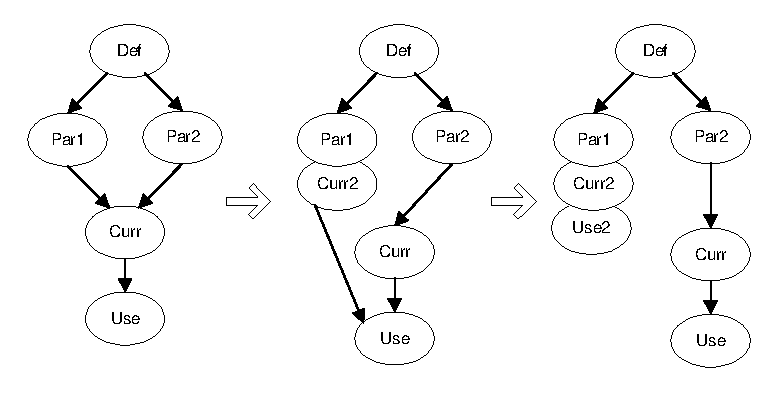
\includegraphics{figures/DuplicateBB.eps}
\centerfigend{fig-duplicateBB}{Duplicating BBs to ensure that each use of
a BasicBlock has a unique definition}

\subsection*{Duplicating a Basic Block}
When the parent of a basic block that needs to be duplicated is a fall-through
or a one-way jump BB, there is only one in-edge, so the RTLs for the current
BB are merely copied
to the end of the list of
RTLs in the parent BB. The parent BB then becomes the same type as the copied
BB, and has the same number of outedges. (The outedges are copied explicitly).
Copying of BBs is done with the clone() member function, to ensure ``deep''
copying. Otherwise, only the pointers to expressions are copied, not the
expressions themselves, and there will be problems when the expressions are
deleted (since the same expression will be deleted twice).

When the parent of a basic block that needs to be duplicated is a two-way BB,
the above method is not suitable. Instead, a new BB is created that is a clone
of the current BB, and the out-edge from the parent to the current BB is
changed to point to the new BB. (Note: this could be the first or ``true''
outedge, or it could be the second or ``false'' outedge). The back end must not
pay attention to the destination of the branch (which remains a faithful
decoding of the original source machine instruction), but rather to where the
BB that the out-edge points to.

In Figure~\ref{fig-duplicate-2way}(a), BB ``Curr'' has a parent BB (``Par1'')
which is a 2-way BB. In this case, a copy of ``Curr'' called ``Curr2'' is made
(Figure~\ref{fig-duplicate-2way}(b)), and the out-edge that used to point to
``Curr'' is changed to point to ``Curr2''. As before, this causes ``Curr2''
to have only one parent, but the successor of both ``Curr'' and ``Curr2''
(the BB ``Use'') now has two parents. When the process is applied to that BB,
we end up with the situation in Figure~\ref{fig-duplicate-2way}(c) where both
``Use'' and ``Use2'' have single paths to the defining BB (not shown).

\centerfigbegin
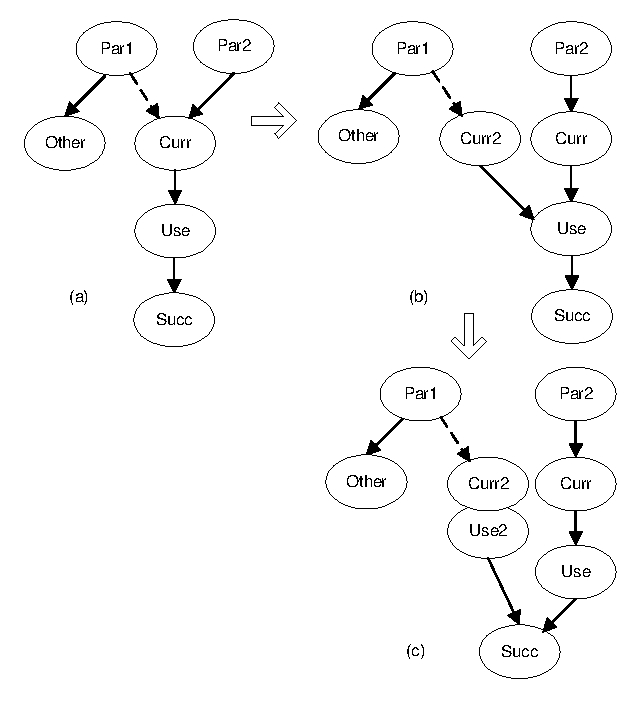
\includegraphics{figures/DuplicateBB2.eps}
\centerfigend{fig-duplicate-2way}{Duplicating a BB with a 2-way parent BB}


\section{Combining Uses and Definitions of Condition Codes}
\label{sec-comb-use-def}

Once unique pairs of CC uses and definitions are found, they must be converted
to a high level equivalent form.

\subsection{Conditional branches and set instructions}

Instructions defining the condition codes are divided into two classes:
``add-like'' and ``subtract-like''. The last RT of the RTL defining the
condition codes (which is expected to be an RTFlagCall\footnote{An object of
class RTFlagCall represents a call to a function that nominally sets the
condition codes for a family of instructions. For example, LOGICALFLAGS sets
the flags for the logical family of instructions.} object) is examined. If
the strings ``SUB'' or ``FFLAG''\footnote{Floating point compares are
considered to be always ``subtract like'', and SETFFLAGS is a typical
flag call function name for setting the floating point condition codes.}
are found in the name of the flag call function, the
instruction defining the condition codes is classified as ``subtract-like''.
Examples include compare instructions, and actual subtract instructions.
Otherwise, the instruction is classified as ``add-like''; examples include
logical instructions such as AND, multiply instructions, and actual ADD
instructions. It is therefore important that the flag call functions are
named appropriately in the SSL file (see section~\ref{sec-srd} for details).

Subtract-like definitions are handled by constructing a high level comparison
expression based on the operands of the comparison or subtraction, and the
type of branch or set instruction. For example,
\begin{verbatim}
 sub a, b, c    # Subtract b from a, result to c
 ...
 sge dest       # Set dest to 1 if "greater than or equals"
\end{verbatim}
has the following high level expression associated with it: ``a $>=$ b''.
The expression is stored in the HLJcond or HLScond object associated
with the RTL that uses the condition code. (The \texttt{setCondExpr} method is
used.)

It is not possible to use the operands directly, since in the final program,
a and b could be modified before the instruction that uses the condition codes.
A mechanism is needed to ``transport'' the condition code information from the
defining instruction to the using instruction. Variables (e.g. ``v12''),
unique to this definition-use pair, are used for this purpose.
Subtract-like definitions of the condition codes
require two such variables; one is needed for each operand.

The variables are copied from expressions passed to the HLFlagCall RT. This
ensures that the correct arguments are copied.

It is important to realise that the result of the subtract is \emph{not}
sufficient to store the result of an unsigned comparison; e.g. v12 = b \gtu\ c
and then branch if v12 \gtu\ 0. For example, 4 \gtu\ 3 and 4-3=1 \gtu\ 0. But
(using 8 bit operands) 204 \gtu\ 3, but 204-3 = 201 == -55, which is a negative
result. (Besides, everything is unsigned greater than 0, other than 0 itself).
The result of the unsigned comparison is in the carry flag, which is a sort of
9th bit of the result.  Therefore, it is not possible in general to save on
variables where unsigned comparisons are involved.

Example pairing:
\begin{verbatim}
10b84:  d0 07 bf e8        ld           [%fp - 24], %o0
10b88:  80 a4 00 08        cmp          %l0, %o0
10b8c:  1a 80 00 04        bgeu         0x10b9c
\end{verbatim}

translates to:

\begin{verbatim}
 v2=*(...);                 # %o0 is mapped to variable v2
 v30=v2;                    # Copy operand 1
 v29=r16;                   # Copy operand 2
 r0=(r16)-(v2);             # The compare, expressed as a subtract
                            #  (result is not used)
 v2=70656;                  # Delay slot instruction
 if (v29 >= v30) goto L11;  # Unsigned comparison
\end{verbatim}

By contrast, add-like definitions need only the result of the operation 
that sets the condition codes. It is an error to find unsigned branches 
or set instructions using the condition codes from an add-like definition. 
For example
\begin{verbatim}
 add a, b, c        # Add a and b, result to c
 ...
 jge dest           # Jump if "greater or equal" to dest
\end{verbatim}
becomes
\begin{verbatim}
c = a + b;
v12 = c;
 ...
if (v12 >= 0) goto dest;
\end{verbatim}

The exception to the above rules are the \texttt{HLJCOND\_JMI} and
\texttt{JLJCOND\_JPOS} branches. These can be used after add-like or after
subtract-like operations (usually a genuine subtract), but since they depend on
the result of the operation, they must be used in an add-like manner.
For example, from
\begin{verbatim}
10bec:  90 a2 20 01        subcc    %o0, 1, %o0
10bf0:  3c bf ff fa        bpos,a   0x10bd8
\end{verbatim}
we generate
\begin{verbatim}
r8=(r8)-(1);
v8=r8;
if ((v8)>=(0)) goto L3;
\end{verbatim}

The analysis code makes the assumptions that the last RT of the RTL defining
the condition codes is a flag call, and (for the above cases) that the second
last RT is an assignment to the result of the operation defining the flags.
Note that if there is a second branch that depends on the above operation,
the second last assignment will be to v8, but it still has the result of the
operation, so it will work correctly.

For other subtract-like operations and branches, it is assumed that the
first two operands (in order) of the flag call are the two operands being
compared (or subtracted). In other words, after
\begin{verbatim}
  x := y - z
  SUBFLAGS(a, b, ...)
\end{verbatim}
it is assumed that a is y and b is z.

As a result of these assumptions, the user is not free to use unusual
semantics in the SSL file. It is hard to imagine the above assumption not
being valid, but it should be kept in mind. In extreme cases, the result of
the operaton may have to be assigned to a temporary variable, then to
either the true destination or another temporary in the second last RT.

\subsection{Assignments that use Condition Codes}

When the instruction using a condition code is an assignment, it is usually
part of an idiomatic sequence.  Two idioms have so far been found and
implemented. The other class of instruction using the carry flag is as part
of multiword arithmetic (e.g. addcc, addx). It may be practical to implement
the multiword arithmetic pairs when the type analysis is able to cope with
variables in two registers; for now, these sequences generate an error message.
This example is from the Solaris 7 /usr/bin/awk:
\begin{verbatim}
142e8:  d2 07 20 00        ld           [%i4], %o1      # Load high half
142ec:  d6 07 20 04        ld           [%i4 + 4], %o3  # Load low half
...
                           # addcc sets flags according to result; add does not
14330:  b4 82 e0 01        addcc        %o3, 1, %i2     # Add 1 to low half
14334:  b2 42 60 00        addx         %o1, 0, %i1     # Add carry to top half
...
142d0:  f2 27 20 00        st           %i1, [%i4]
142d8:  f4 27 20 04        st           %i2, [%i4 + 4]
\end{verbatim}

Here, there are 64 bit integer quantities in the register pairs \%o1:\%o3,
and also \%i1:\%i2 (the colon represents concatenation).

The first idiomatic sequence is: ``compare 0 to a; use carry flag''. Arithmetic
assignment statements using the carry flag need no extra transformation; they
decode to RTLs which use the \%CF register (machine independent carry
flag). For example, \texttt{addx \%g0, 0, \%o3} decodes to
``r[10] := r[0] + 0 + \%CF''. (In the final C output of the translator, \%CF
is represented by the integer variable CF). Therefore, the only transformation
required is to ensure that each use has a unique definition, and to make an
appropriate assignment to \%CF.

Since subtracting any value from zero will generate a carry, unless that value
is zero, comparing 0 to X is equivalent to setting the carry flag only if X
is non-zero. In other words,
compare 0 to X is transformed to ``\%CF = (X != 0)''. An appropriate
assignment RT (i.e. an object of class RTAssgn) is created, and appended to the
list of RTs for the RTL defining the flags. For example:
\begin{verbatim}
10aec:  80 a0 00 0b        cmp          %g0, %o3        # %g0 is always 0
10af0:  94 60 3f ff        subx         %g0, -1, %o2    # Make use of %CF
10af8:  96 40 20 00        addx         %g0, 0, %o3     # Another use of %CF
\end{verbatim}
transforms to
\begin{verbatim}
         # Variable v5 represents register %o3 for this procedure
00010aec *32* r[0] := -v5           # The compare, expressed as a subtract
         *32* %CF := v5 ~= 0        # Generated assignment
         SUBFLAGS( r[0], v5, r[0] )
00010af0 *32* v4 := -%CF + 1        # Register %o2 is held in variable v4
00010af4 *32* v5 := %CF             # Register %o3 is held in variable v5
\end{verbatim}
In C, this becomes
\begin{verbatim}
        r0=-(v5);
        CF=(v5)!=(0);
        v4=(-(CF))+(1);
        v5=CF;
\end{verbatim}


The second idiomatic sequence is similar: ``compare X to Y; use carry flag''.
This is transformed to ``\%CF = X \ltu\ Y'' (where \ltu\ represents ``unsigned
less than''). After subtracting Y from X, a carry will be generated if and only
if Y is greater than x (with both X and Y considered as unsigned quantities).
In other words, after cmp X, Y the carry flag represents the logical expression
X \ltu\ Y.

\section{Complex example}

Despite the apparent simplicity of the above, real code can be surprisingly
complex. The following SPARC code is from the 126.gcc Spec benchmark, generated
from the last 4 lines of C here:

\begin{verbatim}
  int unsignedp = TREE_UNSIGNED (index_type);
  typedef rtx rtx_function ();
  rtx_function *gen_bgt_pat = unsignedp ? gen_bgtu : gen_bgt;
  rtx_function *gen_bge_pat = unsignedp ? gen_bgeu : gen_bge;
  rtx_function *gen_blt_pat = unsignedp ? gen_bltu : gen_blt;
  rtx_function *gen_ble_pat = unsignedp ? gen_bleu : gen_ble;
\end{verbatim}

The addresses of the eight functions (e.g. \texttt{gen\_bgtu}) are set up in
registers like \texttt{\%i2} and stack memory like \texttt{[\%sp + 144]}
in earlier code that is not relevant to the analysis.

\begin{verbatim}
7834c:  80 90 00 1b        orcc         %g0, %i3, %g0
78350:  02 80 00 04        be           0x78360
78354:  a8 10 00 1a        mov          %i2, %l4
78358:  10 80 00 02        ba           0x78360
7835c:  a8 10 00 19        mov          %i1, %l4
78360:  22 80 00 04        be,a    0x78370
78364:  e4 03 a0 90        ld           [%sp + 144], %l2
78368:  10 80 00 02        ba           0x78370
7836c:  e4 03 a0 94        ld           [%sp + 148], %l2
78370:  22 80 00 04        be,a    0x78380
78374:  e2 03 a0 98        ld           [%sp + 152], %l1
78378:  10 80 00 02        ba           0x78380
7837c:  e2 03 a0 9c        ld           [%sp + 156], %l1
78380:  02 80 00 04        be           0x78390
78384:  90 10 00 1c        mov          %i4, %o0
78388:  10 80 00 03        ba           0x78394
7838c:  a0 10 00 1d        mov          %i5, %l0
78390:  e0 03 a0 a0        ld           [%sp + 160], %l0
78394:  92 10 00 15        mov          %l5, %o1
\end{verbatim}

The orcc instruction at the top is the definition for the following conditional
branch, and also three more branches. Because of the two-way BBs between the
definition and the conditional branches, there are a lot of BB duplications
required to translate this code.

There are also several ``orphan'' basic blocks generated as a result of
untangling the delay slots in the above. The code above generates some
23 basic blocks, as shown in Figure~\ref{fig-complex-example}.

\centerfigbegin
{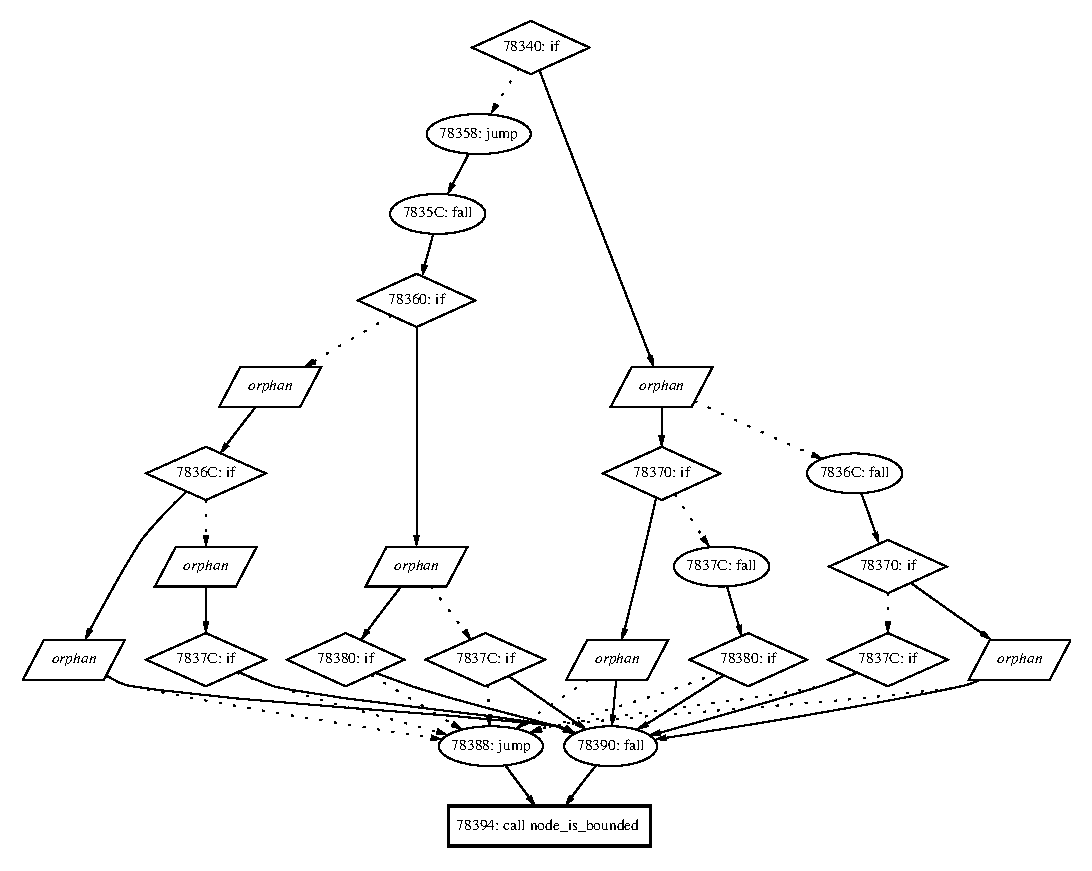
\includegraphics{figures/complex_example.eps}}
\centerfigend{fig-complex-example}{BBs generated for the complex example}
      % matching condition code definitions and uses

  	
\chapter{Transformations of Delayed Transfers of Control}
\label{ch-delay}

{\small
\begin{flushright}
Design: Norman and Cristina [c.98]; Implementation: Mike [c.98-99]; Documentation: Norman, Cristina [Sep 99]
\end{flushright}
}

This chapter is an updated version of Technical Report 440, Department of 
Computer Science and Electrical Engineering, The University of 
Queensland, December 1998.  A more up to date version, including 
application of this algorithm to the removal of PA-RISC delayed branches
will be part of a Sun Microsytems Laboratories Technical Report series  
(expected, early 2002). 
 

% l2h ignore special {% ===> this file was generated automatically by noweave --- better not edit it

%\ifx\afour\undefined
%  \documentclass[letterpaper]{elsart}
%  \let\sizeinfo\relax
%\else 
%  \documentclass[a4paper]{elsart}
%  \special{papersize=210mm,297mm} % put dvips into a4 automagically
%  \def\sizeinfo{A4 }
%\fi

%\usepackage{nchicago}

% l2h substitution bullet *
% l2h substitution and and
% l2h ignore active


\makeatletter
\def\@citex[#1]#2{%
  \let\@citea\@empty
  \@cite{\@for\@citeb:=#2\do
        {\@citea\def\@citea{,\penalty\@m\ }%
         \edef\@citeb{\expandafter\@firstofone\@citeb}%
         \if@filesw\immediate\write\@auxout{\string\citation{\@citeb}}\fi
         \@ifundefined{b@\@citeb}{\mbox{\reset@font\bfseries ?}%
           \G@refundefinedtrue
           \@latex@warning
             {Citation `\@citeb' on page \thepage \space undefined}}%
           {\citebox{\csname b@\@citeb\endcsname}}}}{#1}}
\let\citebox\hbox
\makeatother

\renewcommand\gets{\mathrel{:=}}

\newcommand\opentab{\addtolength{\extrarowheight}}
% l2h ignore catcode ==
% l2h let gdef def

% l2h substitution hatform ^
% l2h ignore markboth {{

% l2h ignore opentab {

% l2h substitution presigmap sigma'
% l2h ignore productionglue
% l2h substitution qquad &nbsp;&nbsp;&nbsp;&nbsp;&nbsp;

\newif\iffullpaper
\fullpapertrue


% l2h argblock calexp E[ ]
% l2h argblock cmd E[ ]


\newcommand\calexp[1]{{\mathcal E}[\![#1]\!]}
\newcommand\cmd[1]{{\mathcal C}[\![#1]\!]}
\newcommand\pc{\mathit{PC}}

%\usepackage{array,tabularx,grammar}

% l2h letenv production quote

\newif\iftr
\trfalse % this is not the tech report

\newcolumntype{Y}{>{\raggedright\arraybackslash}X}


%\usepackage{noweb}
\let\originalprime='
\def\setupcode{\catcode`\ =10 \catcode`\'=12 \mathcode`\'="8000 \regressprime}
{\catcode`\'=\active 
 \makeatletter
 \gdef\regressprime{\def'{^\bgroup\prim@s}}
}
\let\Tt\relax


% l2h substitution div div
% l2h substitution mod mod

\overfullrule=10pt

\noweboptions{shortxref}
\def\nwdocspar{\vskip0pt plus1.5in\penalty-400\vskip0pt plus -1.5in}
%\def\nwdocspar{\par\penalty-1000}
\def\nwendcode{\endtrivlist\endgroup} % ditches filbreak
%\def\nwendcode{\endtrivlist\endgroup\vskip\nwextraglue} % page tuning

\newcommand{\fig}[1]{Figure~\ref{fig:#1}}

\newcommand\sfilbreak[1]{\vskip 0pt plus#1\penalty-200\vskip 0pt plus -#1}

\setcounter{secnumdepth}{2}

\let\orghbox=\hbox
\newcommand\nohbox{\let\hbox=\orghbox\relax}



%% \pagestyle{myheadings}
%% \catcode`\$=10 % make $ a blank space
%% \catcode`\:=10 % make : a blank space
%% \newcommand\rcsrevision{$Revision: 1.4 $}
%% \catcode`\$=3 % dollar sign is math shift
%% \catcode`\:=12
%% \markboth{\rcsrevision: \sizeinfo Draft of \today}{\rcsrevision: \sizeinfo Draft of \today}
%% 
%% \pagestyle{plain}

\def\remark#1{\marginpar{\raggedright\hbadness=10000
        \def\baselinestretch{0.8}\scriptsize
        \it #1\par}}

\let\hatform\overline

\let\nwpphat=\hatform

The fundamental steps in binary translation are
distinguishing code from data, mapping data from source to
target, and translating instructions.
Translating instructions presents few problems, except
when the source instruction set 
has features not present in typical compiler intermediate codes.
The most common such feature is the delayed branch.

Standard code-generation technology can handle delayed branches in the
target language, but not in the source.
Translating delayed branches can involve tricky case
analyses to figure out what happens if there is a branch instruction in
a delay slot.
This chapter presents a disciplined method for deriving such case analyses.
The method identifies problematic cases,
shows the translations for the non-problematic cases, and gives
confidence that all cases are considered.
The method also applies to other tools that analyze machine instructions.

We begin by writing a very simple interpreter for the source machine.
It specifies, at the register-transfer level, how the source machine
executes instructions, including delayed branches. We then transform
the interpreter into an interpreter for a target machine without
delayed branches.
To maintain the semantics of the program being interpreted, we 
simultaneously transform the sequence of source-machine instructions
into a sequence of target-machine instructions.
The transformation of the instructions becomes our
algorithm for binary translation.

We show the translation is correct by using a correspondence between
source and target states, and showing if the source and target
machines begin execution in corresponding states, they reach new
corresponding states in a few instructions.


\renewcommand\opencite[1]{{\let\citebox=\relax\cite{#1}}}

A quick reading of this chapter might suggest that the problem we solve
is trivial.
To build a flow graph representing a binary program,
why not simply convert the delayed branch to a non-delayed branch and
push the instruction in the delay slot along zero, one, or both
sucessor edges?
(The set of successors that should get copies of the instruction in
the delay slot depends on whether the delayed branch
``annuls'' that instruction.)
This simple approach is in fact correct, \emph{except} when the
instruction in the delay slot is itself a delayed branch.
In that case, the ``pushing'' approach fails to execute the
instruction that is the target of the first branch.
The methods in this paper translate this case correctly.
In practice, such cases occur rarely in user code, but they are
recommended in kernel code as a way of returning from interrupts or
otherwise switching contexts \cite[\S B.26]{sparc:architecture}.


\section{Semantic framework}

Rather than translate source-machine instructions directly into target-machine
instructions, we translate source instructions into register transfer
lists (RTLs), transform the RTLs, optimize the RTLs, and translate the
RTLs into target-machine instructions.
RTLs provide a uniform framework that can express source instructions,
target instructions, and their interpretations by the source and
target processors.

\subsection{Register transfer lists}

Our RTL formalism is designed for use in tools and component
generators, and it makes machine-dependent
computation explicit \opencite{ramsey:embedded}.
For this paper, we use a simplified version specified using an imperative syntax:
\begin{production}{rtl}%figure
\optional{\nt{effect} \sequence{\lit\vbar\ \nt{effect}}}
&Multiple assignment
\end{production}
\productionglue
\begin{production}{effect}%figure
\optional{\nt{exp} {{\Tt{}\(\mathbin{\rightarrow}\)}}} \nt{location} := \nt{exp}&
Guarded assignment
\end{production}
\productionglue
\begin{production}{exp}%figure
\term{constant}&Constant
| \nt{location}&Fetch from a location
| \nt{exp} \nt{binop} \nt{exp}&Binary RTL operator
| \nt{operator} \lit( \nt{explist} \lit)&RTL operator
\end{production}
A register transfer list is a list of guarded effects.
Each effect represents the transfer of a value into a storage
location,\footnote{Storage locations represent not only memory but
also registers and other processor state.}
 i.e., a store
operation.
The transfer takes place only if the guard (an expression) evaluates
to \textbf{true}.
Effects in a list take place simultaneously, as in
Dijkstra's multiple-assignment statement; an RTL represents a single
change of state.
%%For example, one RTL can specify a swap instruction without
%%introducing bogus temporaries.

Values are computed by expressions without
side effects.
Eliminating side effects simplifies analysis and transformation.
Expressions may be integer constants, fetches from locations, or
applications of \emph{RTL operators} to lists of expressions.
RTL operators are pure functions on values.

For purposes of this paper, we assume that locations are single cells
in a mutable store, although the RTL formalism supports a more general
view that makes byte order explicit.
\iffalse
Locations may be single cells or aggregates of consecutive
cells within a storage space.
Aggregation generalizes the idea of byte order, specifying a bijection
between a contiguous sequence of $k$ $n$-bit values and a single
$w$-bit value, where $w = kn$.\footnote{$w$ and $n$ are mnemonic for
``wide'' and ``narrow.''}
\fi

\iffullpaper
As an example of a typical RTL, consider a SPARC load instruction
using the displacement 
addressing mode, written in the SPARC  assembly language as
\begin{verbatim}
  ld [%sp-12], %i0
\end{verbatim}
The effect of this load instruction might be written
\nwenddocs{}\nwbegincode{2}\moddef{RTL for sample instruction}\endmoddef\nwstartdeflinemarkup\nwenddeflinemarkup
\(\$r[24] \mathrel{:=} \$m[\$r[14]+{\mathit{sx}}(\mathord{-}12)]\)
\nwendcode{}\nwbegindocs{3}because the stack pointer is register~14 and register \texttt{\%i0} is
register~24.
The notation {\Tt{}\(\$\)}\emph{space}\texttt{[}\emph{address}\texttt{]}
specifies a cell in a mutable store.
The {\Tt{}\({\mathit{sx}}\)} operator sign-extends the 13-bit immediate constant {\Tt{}\(\mathord{-}12\)}
so it can be added to the 32-bit value fetched from register~14.

The load instruction not only loads a value into register~24; it also advances
the program counter to point to the next instruction.
Changing the program counter is intimately connected with branching;
we separate the effect on the
program counter in order to give it special treatment.
\else
\emph{The full paper shows and explains an example RTL.}
\fi

\subsection{Processor state for delayed branches}

A processor executing straight-line code executes one instruction
after another, in sequence.
A delayed-branch instruction causes the processor to depart from that
sequence, but not immediately.
When the processor executes an instruction~{\Tt{}\(I\)} that causes a delayed
branch to a location 
{\Tt{}\({\mathit{target}}\)}, the processor {first} executes {\Tt{}\(I\)}'s successor,
{then} executes the instruction located at {\Tt{}\({\mathit{target}}\)}.
The location holding {\Tt{}\(I\)}'s successor is called {\Tt{}\(I\)}'s ``delay
slot.''
On some machines, like the SPARC,
the instruction~{\Tt{}\(I\)} can
``annul'' its successor, in which case the successor is
\emph{not} executed, but instead the processor stalls for a cycle
before transferring control to {\Tt{}\({\mathit{target}}\)}.

To model delayed branches with annuls, we use
three pieces of processor state:
\begin{itemize}
\item[{}{\Tt{}\({\mathit{PC}}\)}{}] is the program counter, which identifies the
instruction about to be executed.
\item[{}{\Tt{}\({\mathit{nPC}}\)}{}] is the ``next program counter,'' which identifies the
instruction to be executed after the current instruction.
\item[{}{\Tt{}\({\mathit{annul}}\)}{}] is the ``annul status,'' which determines
whether the processor executes the instruction at~{\Tt{}\({\mathit{PC}}\)} or ignores
it.%
\footnote{\iffullpaper
It is crucial to distinguish the {\Tt{}\({\mathit{annul}}\)} status, which is
part of 
the processor state, from the \texttt{a}~bit found in the binary
representations of some branch instructions.
The interpretation of the {\Tt{}\({\mathit{annul}}\)} status is trivial: it tells
directly whether to execute an instruction.
The interpretation of the \texttt{a}~bit (when present) is more involved,
because there are special rules for some instructions.
We abstract away from these special rules by associating with each
instruction~{\Tt{}\(I\)} a predicate~{\Tt{}\(a_I\)} (not necessarily a single bit) that
tells the processor 
whether to annul the instruction's successor.
\else
\emph{The full paper notes the distinction between {\Tt{}\({\mathit{annul}}\)} and the
\texttt{a}~bit found in some branch instructions.}%
\fi
}
\end{itemize}
In this model, a delayed control transfer is represented by an
assignment to~{\Tt{}\({\mathit{nPC}}\)}.
For example, a SPARC call instruction simultaneously
assigns the target address to~{\Tt{}\({\mathit{nPC}}\)}
and the current {\Tt{}\({\mathit{PC}}\)} to register~15:
\nwenddocs{}\nwbegincode{4}\moddef{RTL for call}\endmoddef\nwstartdeflinemarkup\nwenddeflinemarkup
\({\mathit{nPC}} \mathrel{:=} {\mathit{target}} \mathrel{|} \$r[15] \mathrel{:=} {\mathit{PC}}\)
\nwendcode{}\nwbegindocs{5}The {\Tt{}\({\mathit{target}}\)} address in the semantics is
distinct from the \texttt{target} field in the binary representation of the
call instruction.
In the case of the SPARC, we abstract away from the rule that says the
target 
address is computed by extending the \texttt{target} field on the
right with zeroes.

A call transfers control unconditionally; we represent a conditional
branch by a guarded assignment to {\Tt{}\({\mathit{nPC}}\)}.
The \texttt{BNE} (branch not equal) instruction tests the {\Tt{}\(Z\)}~(zero)
bit in the condition codes:
\nwenddocs{}\nwbegincode{6}\moddef{rtl for conditional branch \texttt{BNE}}\endmoddef\nwstartdeflinemarkup\nwenddeflinemarkup
\(\lnot  Z \mathbin{\rightarrow} {\mathit{nPC}} \mathrel{:=} {\mathit{target}}\)
\nwendcode{}\nwbegindocs{7}Again we abstract the computation of the target address relative to
the location of the instruction.
\nwenddocs{}\nwbegindocs{8}\nwdocspar
\subsection{A canonical form of RTLs}
To isolate the part of instruction semantics that is relevant to
control flow, we put RTLs into the following canonical form:
\nwenddocs{}\nwbegincode{9}\moddef{RTL for generic instruction \code{}I\edoc{}}\endmoddef\nwstartdeflinemarkup\nwenddeflinemarkup
\(b_I \mathbin{\rightarrow} {\mathit{nPC}} \mathrel{:=} {\mathit{target}}_I \mathrel{|} {\mathit{annul}} \mathrel{:=} a_I \mathrel{|} I_c\)
\nwendcode{}\nwbegindocs{10}We interpret this form as follows:
\begin{itemize}
\item [{}{\Tt{}\(b_I\)}{}] is a predicate that tells whether {\Tt{}\(I\)}~branches.
It is an \emph{expression}, not a constant or a field of the
instruction.
For non-branching instructions, {\Tt{}\(b_I\)}~is {\Tt{}\(\textbf{false}\)}.
For calls and
unconditional branches, {\Tt{}\(b_I\)} is {\Tt{}\(\textbf{true}\)}.
For conditional branches, {\Tt{}\(b_I\)} is some other expression, the value of
which depends on the state of the machine (e.g., on the values of
the condition codes).
\item [{}{\Tt{}\({\mathit{target}}_I\)}{}] is an {expression} that identifies the
target address to which {\Tt{}\(I\)}~may branch.
(If {\Tt{}\(b_I\)} is {\Tt{}\(\textbf{false}\)}, {\Tt{}\({\mathit{target}}_I\)} is arbitrary.)
For calls and PC-relative branches, {\Tt{}\({\mathit{target}}_I\)} is a constant that
statically identifies a target address.
For indirect branches, {\Tt{}\({\mathit{target}}_I\)} may be a more complex expression,
e.g., one that fetches an address stored in a register.
\item [{}{\Tt{}\(a_I\)}{}] is a predicate that tells whether {\Tt{}\(I\)}~annuls its
successor. 
It is an expression, {not} the value of the \texttt{a}~bit in an
instruction's representation.
For most instructions, {\Tt{}\(a_I\)} is {\Tt{}\(\textbf{false}\)}.
For conditional branches, {\Tt{}\(a_I\)} may be more complicated.
For example,  the SPARC \texttt{BNE} instruction annuls its successor
if the \texttt{a} bit is set and if the branch is not taken, so {\Tt{}\(a_I\)} is
\mbox{{\Tt{}\(\mathtt{a} \ne  0 \land  Z\)}}.
\item [{}{\Tt{}\(I_c\)}{}] is an RTL that represents {\Tt{}\(I\)}'s ``computational
effect.''
{\Tt{}\(I_c\)} may be empty, or it may contain guarded assignments that do
not change {\Tt{}\({\mathit{annul}}\)}, {\Tt{}\({\mathit{nPC}}\)}, or {\Tt{}\({\mathit{PC}}\)}.
Typical RISC instructions change control flow or perform computation,
but not both, so {\Tt{}\(I_c\)} tends to be non-empty only when {\Tt{}\(b_I\)}
and {\Tt{}\(a_I\)} are {\Tt{}\(\textbf{false}\)}.
On CISC architectures, however, an instruction like ``decrement and
skip if zero'' might have both  non-empty {\Tt{}\(I_c\)} (the decrement) and
a nontrivial {\Tt{}\(b_I\)} (the test for zero).
\end{itemize}
An instruction can be expressed in this canonical form if, when
executed, it branches to
at most one {\Tt{}\({\mathit{target}}\)}.%
\footnote{And of course if the machine uses delayed branches.}
This is true of all instructions on all architectures with which we
are 
familiar, including indirect-branch instructions (although the value
 of {\Tt{}\({\mathit{target}}\)} may be different on different executions of an indirect
branch).

Here are a few example RTLs in canonical form;
SPARC assembly language appears on the left, RTLs on the right.
{\Tt{}\textbf{skip}} is the empty~RTL.
\begin{quote}%figure
\begin{tabular}{@{}ll@{}}
\multicolumn2{@{}l}{\texttt{add rs1, rs2, rd}}\\
\multicolumn2{@{}l}{\qquad  
{\Tt{}\(\textbf{false} \mathbin{\rightarrow} {\mathit{nPC}} \mathrel{:=} {\mathit{any}} \mathrel{|} {\mathit{annul}} \mathrel{:=} \textbf{false} \mathrel{|} \$r[\mathtt{rd}] \mathrel{:=} \$r[\mathtt{rs1}] + \$r[\mathtt{rs2}]\)}}\\
\texttt{ba,a addr}&{\Tt{}\(\textbf{true} \mathbin{\rightarrow} {\mathit{nPC}} \mathrel{:=} \mathtt{addr} \mathrel{|} {\mathit{annul}} \mathrel{:=} \textbf{true} \mathrel{|}\){\ }\textbf{skip}}\\
\texttt{call addr}&{\Tt{}\(\textbf{true} \mathbin{\rightarrow} {\mathit{nPC}} \mathrel{:=} \mathtt{addr} \mathrel{|} {\mathit{annul}} \mathrel{:=} \textbf{false} \mathrel{|} \$r[15] \mathrel{:=} {\mathit{PC}}\)}\\
\end{tabular}\kern-20pt
\end{quote}

\nwenddocs{}\nwbegindocs{11}\nwdocspar
\subsection{Instruction decoding and execution on two platforms}
Given this canonical form for instructions, we represent instruction
decoding using a {\Tt{}\textbf{let}}-binding notation:
\nwenddocs{}\nwbegincode{12}\moddef{instruction decoding}\endmoddef\nwstartdeflinemarkup\nwenddeflinemarkup
\textbf{let}{\ }\((b_I \mathbin{\rightarrow} {\mathit{nPC}} \mathrel{:=} {\mathit{target}}_I \mathrel{|} {\mathit{annul}} \mathrel{:=} a_I \mathrel{|} I_c) \equiv  {\mathit{src}}[{\mathit{PC}}]\)
\textbf{in}{\ }{\ }\(\ldots\)
\textbf{end}
\nwendcode{}\nwbegindocs{13}The {\Tt{}\textbf{let}} construct binds {\Tt{}\(b_I\)}, {\Tt{}\({\mathit{target}}_I\)},
{\Tt{}\(a_I\)}, and {\Tt{}\(I_c\)}, which together determine the
semantics of the instruction~{\Tt{}\(I\)} found in the source memory~{\Tt{}\({\mathit{src}}\)}.
\iffullpaper
This {\Tt{}\textbf{let}}-binding represents not only the process of using the
binary representation to identify the instruction and its operands,
but also the abstraction from that representation into the RTL semantics.
This abstraction from binary representation to semantics can be done
statically, at 
binary-translation time; it can even be automated based on a
combination of machine descriptions
\opencite{ramsey:specifying,ramsey:embedded}.
\fi
\nwenddocs{}\nwbegindocs{14}\nwdocspar
The source-machine execution loop
decodes an instruction and executes it as follows:
\nwenddocs{}\nwbegincode{15}\moddef{sparc execution loop}\endmoddef\nwstartdeflinemarkup\nwenddeflinemarkup
\textbf{fun}{\ }\({\mathit{loop}} () \equiv \)
{\ }{\ }\textbf{let}{\ }\((b_I \mathbin{\rightarrow} {\mathit{nPC}} \mathrel{:=} {\mathit{target}}_I \mathrel{|} {\mathit{annul}} \mathrel{:=} a_I \mathrel{|} I_c) \equiv  {\mathit{src}}[{\mathit{PC}}]\)
{\ }{\ }\textbf{in}{\ }{\ }\textbf{if}{\ }\({\mathit{annul}}\){\ }\textbf{then}
{\ }{\ }{\ }{\ }{\ }{\ }{\ }{\ }{\ }\({\mathit{PC}} \mathrel{:=} {\mathit{nPC}} \mathrel{|} {\mathit{nPC}} \mathrel{:=} {\mathit{succ}}_s({\mathit{nPC}}) \mathrel{|} {\mathit{annul}} \mathrel{:=} \textbf{false}\)
{\ }{\ }{\ }{\ }{\ }{\ }\textbf{else}{\ }\textbf{if}{\ }\([\![b_I]\!]\){\ }\textbf{then}
{\ }{\ }{\ }{\ }{\ }{\ }{\ }{\ }{\ }\({\mathit{PC}} \mathrel{:=} {\mathit{nPC}} \mathrel{|} {\mathit{nPC}} \mathrel{:=} [\![{\mathit{target}}_I]\!]  \mathrel{|} [\![I_c]\!] \mathrel{|} {\mathit{annul}} \mathrel{:=} [\![a_I]\!]\)
{\ }{\ }{\ }{\ }{\ }{\ }\textbf{else}
{\ }{\ }{\ }{\ }{\ }{\ }{\ }{\ }{\ }\({\mathit{PC}} \mathrel{:=} {\mathit{nPC}} \mathrel{|} {\mathit{nPC}} \mathrel{:=} {\mathit{succ}}_s({\mathit{nPC}}) \mathrel{|} [\![I_c]\!] \mathrel{|} {\mathit{annul}} \mathrel{:=} [\![a_I]\!]\)
{\ }{\ }{\ }{\ }{\ }{\ }\textbf{fi}
{\ }{\ }{\ }{\ }{\ }{\ }\(; {\mathit{loop}}()\)
{\ }{\ }\textbf{end}
\nwendcode{}\nwbegindocs{16}We specify the repeated execution of the processor loop as a tail
call, rather than as a loop, because that simplifies the
program transformations to follow.
\nwenddocs{}\nwbegindocs{17}\nwdocspar
The notation {\Tt{}\([\![\bullet ]\!]\)} represents execution; for example,
{\Tt{}\([\![b_I]\!]\)} is the value of the branch condition, given the current
state of the machine.
Executing the computational effect {\Tt{}\([\![I_c]\!]\)} changes the state of the machine.
\nwenddocs{}\nwbegindocs{18}\nwdocspar
The function {\Tt{}\({\mathit{succ}}_s\)} abstracts over the details of identifying
the successor instruction on the source machine; {\Tt{}\({\mathit{succ}}_t\)} finds the
successor on the target machine.
In both cases, {\Tt{}\({\mathit{succ}}\)} is computed as part of instruction decoding.
\nwenddocs{}\nwbegindocs{19}\nwdocspar
Our example target, the Pentium, has neither delayed branches nor
annulling, so it has a simpler canonical form and a simpler execution
loop:
\nwenddocs{}\nwbegincode{20}\moddef{Pentium execution loop}\endmoddef\nwstartdeflinemarkup\nwenddeflinemarkup
\textbf{fun}{\ }\({\mathit{simple}} () \equiv \)
{\ }{\ }\textbf{let}{\ }\((b_I \mathbin{\rightarrow} {\mathit{PC}} \mathrel{:=} {\mathit{target}}_I \mathrel{|} I_c) \equiv  {\mathit{tgt}}[{\mathit{PC}}]\)
{\ }{\ }\textbf{in}{\ }{\ }\textbf{if}{\ }\([\![b_I]\!]\){\ }\textbf{then}
{\ }{\ }{\ }{\ }{\ }{\ }{\ }{\ }\({\mathit{PC}} \mathrel{:=} [\![{\mathit{target}}_I]\!] \mathrel{|} [\![I_c]\!]\)
{\ }{\ }{\ }{\ }{\ }{\ }\textbf{else}
{\ }{\ }{\ }{\ }{\ }{\ }{\ }{\ }\({\mathit{PC}} \mathrel{:=} {\mathit{succ}}_t({\mathit{PC}}) \mathrel{|} [\![I_c]\!]\)
{\ }{\ }{\ }{\ }{\ }{\ }\textbf{fi}
{\ }{\ }{\ }{\ }{\ }{\ }\(; {\mathit{simple}}()\)
{\ }{\ }\textbf{end}
\nwendcode{}\nwbegindocs{21}\nwdocspar




\subsection{Strategy for translating delayed branches}

Both our formalism and
the SPARC architecture manual give a clear semantics of delayed
branches in terms of {\Tt{}\({\mathit{PC}}\)}, {\Tt{}\({\mathit{nPC}}\)}, and {\Tt{}\({\mathit{annul}}\)}.
To get an efficient target program, however, we wish \emph{not} to
represent the source {\Tt{}\({\mathit{PC}}\)}, {\Tt{}\({\mathit{nPC}}\)}, and {\Tt{}\({\mathit{annul}}\)} explicitly, but to
make all three \emph{implicit} in the value of the target~{\Tt{}\({\mathit{PC}}\)}.
How to do this based on the information in the architecture manual is
not immediately obvious, but our semantic framework enables a new technique.
We transform {\Tt{}\({\mathit{loop}}\)}, eliminating {\Tt{}\({\mathit{nPC}}\)} and {\Tt{}\({\mathit{annul}}\)} wherever
possible, so that (almost all of) {\Tt{}\({\mathit{loop}}\)} can be expressed using only
the~{\Tt{}\({\mathit{PC}}\)}.
%%This transformation leads to suitable changes in the sequence of
%%instructions executed, thus guiding a transformation from {\Tt{}\({\mathit{src}}\)} to {\Tt{}\({\mathit{tgt}}\)}.
%%This latter transformation is an algorithm for binary translation of
%%delayed-branch instructions.


% l2h substitution src s-sigma-
% l2h substitution tgt t-sigma-

\newcommand\presigma[1]{\mathord{{}^{#1}\sigma}}
\newcommand\presigmap[1]{\mathord{{}^{#1}\sigma'}}
\newcommand\src[1]{\presigma{s}_{#1}}
\newcommand\tgt[1]{\presigma{t}_{#1}}


\section{Transforming the execution loop}

We wish to develop a translation function that we can point at a
location {\Tt{}\({\mathit{src}}[{\mathit{pc}}_s]\)} and that will produce suitable instructions at a
corresponding target location {\Tt{}\({\mathit{tgt}}[{\mathit{pc}}_t]\)}.
We cannot simply have {\Tt{}\({\mathit{pc}}_t = {\mathit{pc}}_s\)}; source program counters
cannot be identical to target program counters, because 
source and target instruction sequences may be different sizes.
During translation, we build {\Tt{}\({\mathit{codemap}}\)}, a map that relates program
counters on the two machines, so {\Tt{}\({\mathit{pc}}_t = {\mathit{codemap}}({\mathit{pc}}_s)\)}.

We assume that
when the source processor starts executing code at {\Tt{}\({\mathit{src}}[{\mathit{pc}}_s]\)}, it
is not in the middle of a delayed
or annulled branch, or formally,
\begin{quote}
{\Tt{}\({\mathit{annul}} = \textbf{false} \land  {\mathit{nPC}} = {\mathit{succ}}_s({\mathit{PC}})\)}.
\end{quote}
Software conventions guarantee that
the processor will be in such a state at a program's start location
and at procedure entry points.
\nwenddocs{}\nwbegindocs{22}\nwdocspar
We begin our transformation by
defining a function {\Tt{}\({\mathit{stable}}\)} that can be substituted for {\Tt{}\({\mathit{loop}}\)}
whenever {\Tt{}\({\mathit{annul}} = \textbf{false} \land  {\mathit{nPC}} = {\mathit{succ}}_s({\mathit{PC}})\)}.
\nwenddocs{}\nwbegincode{23}\moddef{stable execution loop}\endmoddef\nwstartdeflinemarkup\nwenddeflinemarkup
\textbf{fun}{\ }\({\mathit{stable}} () \equiv \)
{\ }{\ }\({\mathit{annul}} \mathrel{:=} \textbf{false} \mathrel{|} {\mathit{nPC}} \mathrel{:=} {\mathit{succ}}_s({\mathit{PC}});\)
{\ }{\ }\textbf{let}{\ }\((b_I \mathbin{\rightarrow} {\mathit{nPC}} \mathrel{:=} {\mathit{target}}_I \mathrel{|} {\mathit{annul}} \mathrel{:=} a_I \mathrel{|} I_c) \equiv  {\mathit{src}}[{\mathit{PC}}]\)
{\ }{\ }\textbf{in}{\ }{\ }\textbf{if}{\ }\({\mathit{annul}}\){\ }\textbf{then}
{\ }{\ }{\ }{\ }{\ }{\ }{\ }{\ }{\ }\({\mathit{PC}} \mathrel{:=} {\mathit{nPC}} \mathrel{|} {\mathit{nPC}} \mathrel{:=} {\mathit{succ}}_s({\mathit{nPC}}) \mathrel{|} {\mathit{annul}} \mathrel{:=} \textbf{false}\)
{\ }{\ }{\ }{\ }{\ }{\ }\textbf{else}{\ }\textbf{if}{\ }\([\![b_I]\!]\){\ }\textbf{then}
{\ }{\ }{\ }{\ }{\ }{\ }{\ }{\ }{\ }\({\mathit{PC}} \mathrel{:=} {\mathit{nPC}} \mathrel{|} {\mathit{nPC}} \mathrel{:=} [\![{\mathit{target}}_I]\!]  \mathrel{|} [\![I_c]\!] \mathrel{|} {\mathit{annul}} \mathrel{:=} [\![a_I]\!]\)
{\ }{\ }{\ }{\ }{\ }{\ }\textbf{else}
{\ }{\ }{\ }{\ }{\ }{\ }{\ }{\ }{\ }\({\mathit{PC}} \mathrel{:=} {\mathit{nPC}} \mathrel{|} {\mathit{nPC}} \mathrel{:=} {\mathit{succ}}_s({\mathit{nPC}}) \mathrel{|} [\![I_c]\!] \mathrel{|} {\mathit{annul}} \mathrel{:=} [\![a_I]\!]\)
{\ }{\ }{\ }{\ }{\ }{\ }\textbf{fi}
{\ }{\ }{\ }{\ }{\ }{\ }\(; {\mathit{loop}}()\)
{\ }{\ }\textbf{end}
\nwendcode{}\nwbegindocs{24}\nwdocspar
\iftr
We move the initial assignment inside the {\Tt{}\textbf{let}}, and we distribute
the tail call to {\Tt{}\({\mathit{loop}}\)} over the arms of the {\Tt{}\textbf{if}}.
\nwenddocs{}%
%
%
%
%
%
%
%
%
%
%
%
%
%
%
\nwbegindocs{26}\nwdocspar
We drop the first arm of the {\Tt{}\textbf{if}}, because {\Tt{}\({\mathit{annul}}\)} is always
false.
We expand the final arm by inserting a test on {\Tt{}\([\![a_I]\!]\)}.
\nwenddocs{}%
%
%
%
%
%
%
%
%
%
%
%
%
%
%
\nwbegindocs{28}\nwdocspar
The last arm of the {\Tt{}\textbf{if}} shows the proper translation of an
instruction that neither branches nor annuls.
We can substitute {\Tt{}\({\mathit{stable}}\)} for {\Tt{}\({\mathit{loop}}\)}, then drop the assignments
to {\Tt{}\({\mathit{annul}}\)} and {\Tt{}\({\mathit{nPC}}\)}, because they don't reach any uses.
Finally, we propagate the initial definition of {\Tt{}\({\mathit{nPC}}\)} to its uses.
(This should be rewritten in a final TR.)
\nwenddocs{}%
%
%
%
%
%
%
%
%
%
%
%
%
%
%
\nwbegindocs{30}\nwdocspar
The next steps are to drop the dead assignments to {\Tt{}\({\mathit{annul}}\)} and
{\Tt{}\({\mathit{nPC}}\)}, and
\fi
We do not show every step in the
transformation of {\Tt{}\({\mathit{stable}}\)}.
The first transformations move the initial
assignments inside the {\Tt{}\textbf{let}}, propagate (by forward substitution)
the assignments to {\Tt{}\({\mathit{annul}}\)} and {\Tt{}\({\mathit{nPC}}\)},
move {\Tt{}\({\mathit{loop}}\)} inside the {\Tt{}\textbf{if}},  replace {\Tt{}\({\mathit{loop}}\)}
with {\Tt{}\({\mathit{stable}}\)} where possible, and drop the (now dead)
assignments.
The result is:
\nwenddocs{}\nwbegincode{31}\moddef{stable execution loop}\plusendmoddef\nwstartdeflinemarkup\nwenddeflinemarkup
\textbf{fun}{\ }\({\mathit{stable}} () \equiv \)
{\ }{\ }\textbf{let}{\ }\((b_I \mathbin{\rightarrow} {\mathit{nPC}} \mathrel{:=} {\mathit{target}}_I \mathrel{|} {\mathit{annul}} \mathrel{:=} a_I \mathrel{|} I_c) \equiv  {\mathit{src}}[{\mathit{PC}}]\)
{\ }{\ }\textbf{in}{\ }{\ }\textbf{if}{\ }\([\![b_I]\!]\){\ }\textbf{then}
{\ }{\ }{\ }{\ }{\ }{\ }{\ }{\ }{\ }\({\mathit{PC}} \mathrel{:=} {\mathit{succ}}_s({\mathit{PC}}) \mathrel{|} {\mathit{nPC}} \mathrel{:=} [\![{\mathit{target}}_I]\!]  \mathrel{|} [\![I_c]\!] \mathrel{|} {\mathit{annul}} \mathrel{:=} [\![a_I]\!]\)
{\ }{\ }{\ }{\ }{\ }{\ }{\ }{\ }{\ }\(; {\mathit{loop}}()\)
{\ }{\ }{\ }{\ }{\ }{\ }\textbf{else}{\ }\textbf{if}{\ }\([\![a_I]\!]\){\ }\textbf{then}
{\ }{\ }{\ }{\ }{\ }{\ }{\ }{\ }{\ }\({\mathit{PC}} \mathrel{:=} {\mathit{succ}}_s({\mathit{PC}}) \mathrel{|} {\mathit{nPC}} \mathrel{:=} {\mathit{succ}}_s({\mathit{succ}}_s({\mathit{PC}})) \mathrel{|} [\![I_c]\!] \mathrel{|} {\mathit{annul}} \mathrel{:=} \textbf{true}\)
{\ }{\ }{\ }{\ }{\ }{\ }{\ }{\ }{\ }\(; {\mathit{loop}}()\)
{\ }{\ }{\ }{\ }{\ }{\ }\textbf{else}
{\ }{\ }{\ }{\ }{\ }{\ }{\ }{\ }{\ }\({\mathit{PC}} \mathrel{:=} {\mathit{succ}}_s({\mathit{PC}}) \mathrel{|} [\![I_c]\!]\)
{\ }{\ }{\ }{\ }{\ }{\ }{\ }{\ }{\ }\(; {\mathit{stable}}()\)
{\ }{\ }{\ }{\ }{\ }{\ }\textbf{fi}
{\ }{\ }\textbf{end}
\nwendcode{}\nwbegindocs{32}%
\iftr
\else 
The last arm of the {\Tt{}\textbf{if}} shows the execution of an
instruction that never branches or annuls.
It corresponds to
the execution of a similar instruction on the {\Tt{}\({\mathit{simple}}\)} target.
\fi
\nwenddocs{}\nwbegindocs{33}\nwdocspar

The next step is to unfold {\Tt{}\({\mathit{loop}}\)} in the first
and second arms of the {\Tt{}\textbf{if}} statement. 
In the second arm, {\Tt{}\({\mathit{annul}}\)} is {\Tt{}\(\textbf{true}\)}, so the call to {\Tt{}\({\mathit{loop}}()\)} can
be replaced by
{\Tt{}\({\mathit{PC}} \mathrel{:=} {\mathit{nPC}}; {\mathit{nPC}} \mathrel{:=} {\mathit{succ}}_s({\mathit{nPC}}); {\mathit{stable}}()\)}.
The definition of {\Tt{}\({\mathit{stable}}\)} reduces to
\iftr
\nwenddocs{}%
%
%
%
%
%
%
%
%
%
%
%
%
%
%
%
%
%
%
%
%
%
%
%
%
%
\nwbegindocs{35}\nwdocspar
We now simplify {\Tt{}\({\mathit{stable}}\)} in two ways.
We encapsulate the first branch of the {\Tt{}\textbf{if}} in the chunk 
{\Tt{}\LA{}case where \code{}I\edoc{} branches\RA{}}, and we simplify the
second branch.
Reasonable care is required when substituting forward the value
({\Tt{}\({\mathit{succ}}_s({\mathit{succ}}_s({\mathit{PC}}))\)}) of {\Tt{}\({\mathit{nPC}}\)}, because the 
RTL that assigns to {\Tt{}\({\mathit{nPC}}\)} also assigns to {\Tt{}\({\mathit{PC}}\)}.
Moreover, because the values bound in the {\Tt{}\textbf{let}} don't reach any
uses, the entire {\Tt{}\textbf{let}} goes away.
Finally, the call to {\Tt{}\({\mathit{loop}}\)} can be replaced by a call to {\Tt{}\({\mathit{stable}}\)},
and the dead assignments to {\Tt{}\({\mathit{annul}}\)} and {\Tt{}\({\mathit{nPC}}\)} dropped.
\fi
\nwenddocs{}\nwbegincode{36}\moddef{stable execution loop}\plusendmoddef\nwstartdeflinemarkup\nwenddeflinemarkup
\textbf{fun}{\ }\({\mathit{stable}} () \equiv \)
{\ }{\ }\textbf{let}{\ }\((b_I \mathbin{\rightarrow} {\mathit{nPC}} \mathrel{:=} {\mathit{target}}_I \mathrel{|} {\mathit{annul}} \mathrel{:=} a_I \mathrel{|} I_c) \equiv  {\mathit{src}}[{\mathit{PC}}]\)
{\ }{\ }\textbf{in}{\ }{\ }\textbf{if}{\ }\([\![b_I]\!]\){\ }\textbf{then}
{\ }{\ }{\ }{\ }{\ }{\ }{\ }{\ }{\ }\LA{}case where \code{}I\edoc{} branches\RA{}
{\ }{\ }{\ }{\ }{\ }{\ }\textbf{else}{\ }\textbf{if}{\ }\([\![a_I]\!]\){\ }\textbf{then}
{\ }{\ }{\ }{\ }{\ }{\ }{\ }{\ }{\ }\({\mathit{PC}} \mathrel{:=} {\mathit{succ}}_s({\mathit{succ}}_s({\mathit{PC}})) \mathrel{|} [\![I_c]\!]\)
{\ }{\ }{\ }{\ }{\ }{\ }{\ }{\ }{\ }\(; {\mathit{stable}}()\)
{\ }{\ }{\ }{\ }{\ }{\ }\textbf{else}
{\ }{\ }{\ }{\ }{\ }{\ }{\ }{\ }{\ }\({\mathit{PC}} \mathrel{:=} {\mathit{succ}}_s({\mathit{PC}}) \mathrel{|} [\![I_c]\!]\)
{\ }{\ }{\ }{\ }{\ }{\ }{\ }{\ }{\ }\(; {\mathit{stable}}()\)
{\ }{\ }{\ }{\ }{\ }{\ }\textbf{fi}
{\ }{\ }\textbf{end}
\nwendcode{}\nwbegindocs{37}where the interesting case is
\nwenddocs{}\nwbegincode{38}\moddef{case where \code{}I\edoc{} branches}\endmoddef\nwstartdeflinemarkup\nwenddeflinemarkup
\({\mathit{PC}} \mathrel{:=} {\mathit{succ}}_s({\mathit{PC}}) \mathrel{|} {\mathit{nPC}} \mathrel{:=} [\![{\mathit{target}}_I]\!]  \mathrel{|} [\![I_c]\!] \mathrel{|} {\mathit{annul}} \mathrel{:=} [\![a_I]\!];\)
\textbf{let}{\ }\((b_{I'} \mathbin{\rightarrow} {\mathit{nPC}} \mathrel{:=} {\mathit{target}}_{I'} \mathrel{|} {\mathit{annul}} \mathrel{:=} a_{I'} \mathrel{|} {I'}_c) \equiv  {\mathit{src}}[{\mathit{PC}}]\)
\textbf{in}{\ }{\ }\textbf{if}{\ }\({\mathit{annul}}\){\ }\textbf{then}
{\ }{\ }{\ }{\ }{\ }{\ }{\ }\({\mathit{PC}} \mathrel{:=} {\mathit{nPC}} \mathrel{|} {\mathit{nPC}} \mathrel{:=} {\mathit{succ}}_s({\mathit{nPC}}) \mathrel{|} {\mathit{annul}} \mathrel{:=} \textbf{false}\)
{\ }{\ }{\ }{\ }\textbf{else}{\ }\textbf{if}{\ }\([\![b_{I'}]\!]\){\ }\textbf{then}
{\ }{\ }{\ }{\ }{\ }{\ }{\ }\({\mathit{PC}} \mathrel{:=} {\mathit{nPC}} \mathrel{|} {\mathit{nPC}} \mathrel{:=} [\![{\mathit{target}}_{I'}]\!]  \mathrel{|} [\![{I'}_c]\!] \mathrel{|} {\mathit{annul}} \mathrel{:=} [\![a_{I'}]\!]\)
{\ }{\ }{\ }{\ }\textbf{else}
{\ }{\ }{\ }{\ }{\ }{\ }{\ }\({\mathit{PC}} \mathrel{:=} {\mathit{nPC}} \mathrel{|} {\mathit{nPC}} \mathrel{:=} {\mathit{succ}}_s({\mathit{nPC}}) \mathrel{|} [\![{I'}_c]\!] \mathrel{|} {\mathit{annul}} \mathrel{:=} [\![a_{I'}]\!]\)
{\ }{\ }{\ }{\ }\textbf{fi}
{\ }{\ }{\ }{\ }\(; {\mathit{loop}}()\)
\textbf{end}
\nwendcode{}\nwbegindocs{39}\nwdocspar
Transformation proceeds by combining these two fragments, moving the
{\Tt{}\textbf{let}}s together, and flattening the nested {\Tt{}\textbf{if}} statements.
We then use ``The Trick'' from partial evaluation \opencite{danvy:eta}:
whenever  {\Tt{}\([\![a_I]\!]\)}~is free in a statement~{\Tt{}\(S\)}, we
replace~{\Tt{}\(S\)} with {\Tt{}\textbf{if}{\ }\([\![a_I]\!]\)}{\Tt{}{\ }\textbf{then}{\ }\(S\){\ }\textbf{else}{\ }\(S\){\ }\textbf{fi}}.
The Trick enables us to replace several calls to {\Tt{}\({\mathit{loop}}\)} with calls
to {\Tt{}\({\mathit{stable}}\)}.
\iftr
Move {\Tt{}\textbf{let}} outside, and propagate definitions to uses.
\nwenddocs{}%
%
%
%
%
%
%
%
%
%
%
%
\nwbegindocs{41}\nwdocspar
Eliminate dead code, and distribute {\Tt{}\({\mathit{loop}}\)} over the arms of the
{\Tt{}\textbf{if}}.
\nwenddocs{}%
%
%
%
%
%
%
%
%
%
%
%
%
%
\nwbegindocs{43}\nwdocspar
Put in {\Tt{}\({\mathit{stable}}\)}
\nwenddocs{}%
%
%
%
%
%
%
%
%
%
%
%
%
%
\nwbegindocs{45}\nwdocspar
\par\bigskip\hrule\bigskip
\def\nwdocspar{\vskip0pt plus2.5in\penalty-200\vskip0pt plus -2.5in}
Re-expand.
\nwenddocs{}%
%
%
%
%
%
%
%
%
%
%
%
%
%
%
%
%
%
%
%
%
%
%
%
%
\nwbegindocs{47}\nwdocspar
Combine {\Tt{}\textbf{let}}s, and flatten {\Tt{}\textbf{if}}.
Also, make conditions more explicit.
\nwenddocs{}%
%
%
%
%
%
%
%
%
%
%
%
%
%
%
%
%
%
%
%
%
%
%
%
\nwbegindocs{49}\nwdocspar
\nwenddocs{}\nwbegindocs{50}\nwdocspar
Insert tests on {\Tt{}\(a_{I'}\)}.
\nwenddocs{}%
%
%
%
%
%
%
%
%
%
%
%
%
%
%
%
%
%
%
%
%
%
%
%
%
%
%
%
%
%
%
%
\nwbegindocs{52}\nwdocspar
This body has four calls to~{\Tt{}\({\mathit{loop}}\)}.
The fourth call satisfies the preconditions for using {\Tt{}\({\mathit{stable}}\)}.
The first and third are made when {\Tt{}\({\mathit{annul}}\)} is true, in which case
{\Tt{}\({\mathit{loop}}\)} can be unfolded once and turned into {\Tt{}\({\mathit{stable}}\)}.
Simplification therefore leaves a version of {\Tt{}\({\mathit{stable}}\)} in which only
one case requires a call to~{\Tt{}\({\mathit{loop}}\)}.
\fi
The result is
\nwenddocs{}\nwbegincode{53}\moddef{stable execution loop}\plusendmoddef\nwstartdeflinemarkup\nwenddeflinemarkup
\textbf{fun}{\ }\({\mathit{stable}} () \equiv \)
{\ }{\ }\textbf{let}{\ }\((b_I  \mathbin{\rightarrow} {\mathit{nPC}} \mathrel{:=} {\mathit{target}}_I  \mathrel{|} {\mathit{annul}} \mathrel{:=} a_I  \mathrel{|} I_c)  \equiv  {\mathit{src}}[{\mathit{PC}}]\)
{\ }{\ }{\ }{\ }{\ }{\ }\((b_{I'} \mathbin{\rightarrow} {\mathit{nPC}} \mathrel{:=} {\mathit{target}}_{I'} \mathrel{|} {\mathit{annul}} \mathrel{:=} a_{I'} \mathrel{|} {I'}_c) \equiv  {\mathit{src}}[{\mathit{succ}}_s({\mathit{PC}})]\)
{\ }{\ }\textbf{in}{\ }{\ }\textbf{if}{\ }\([\![b_I]\!] \land  [\![a_I]\!]\){\ }\textbf{then}
{\ }{\ }{\ }{\ }{\ }{\ }{\ }{\ }{\ }\([\![I_c]\!];\)
{\ }{\ }{\ }{\ }{\ }{\ }{\ }{\ }{\ }\({\mathit{PC}} \mathrel{:=} [\![{\mathit{target}}_I]\!]\)
{\ }{\ }{\ }{\ }{\ }{\ }{\ }{\ }{\ }\(; {\mathit{stable}}()\)
{\ }{\ }{\ }{\ }{\ }{\ }\textbf{else}{\ }\textbf{if}{\ }\([\![b_I]\!] \land  \lnot  [\![a_I]\!] \land  [\![b_{I'}]\!] \land  [\![a_{I'}]\!]\){\ }\textbf{then}
{\ }{\ }{\ }{\ }{\ }{\ }{\ }{\ }{\ }\([\![I_c]\!];\)
{\ }{\ }{\ }{\ }{\ }{\ }{\ }{\ }{\ }\([\![{I'}_c]\!];\)
{\ }{\ }{\ }{\ }{\ }{\ }{\ }{\ }{\ }\({\mathit{PC}} \mathrel{:=} [\![{\mathit{target}}_{I'}]\!]\)
{\ }{\ }{\ }{\ }{\ }{\ }{\ }{\ }{\ }\(; {\mathit{stable}}()\)
{\ }{\ }{\ }{\ }{\ }{\ }\textbf{else}{\ }\textbf{if}{\ }\([\![b_I]\!] \land  \lnot  [\![a_I]\!] \land  [\![b_{I'}]\!] \land  \lnot  [\![a_{I'}]\!]\){\ }\textbf{then}
{\ }{\ }{\ }{\ }{\ }{\ }{\ }{\ }{\ }\([\![I_c]\!];\)
{\ }{\ }{\ }{\ }{\ }{\ }{\ }{\ }{\ }\({\mathit{PC}} \mathrel{:=} [\![{\mathit{target}}_I]\!] \mathrel{|} {\mathit{nPC}} \mathrel{:=} [\![{\mathit{target}}_{I'}]\!]  \mathrel{|} [\![{I'}_c]\!] \mathrel{|} {\mathit{annul}} \mathrel{:=} \textbf{false}\)
{\ }{\ }{\ }{\ }{\ }{\ }{\ }{\ }{\ }\(; {\mathit{loop}}()\)
{\ }{\ }{\ }{\ }{\ }{\ }\textbf{else}{\ }\textbf{if}{\ }\([\![b_I]\!] \land  \lnot  [\![a_I]\!] \land  \lnot  [\![b_{I'}]\!] \land  [\![a_{I'}]\!]\){\ }\textbf{then}
{\ }{\ }{\ }{\ }{\ }{\ }{\ }{\ }{\ }\([\![I_c]\!];\)
{\ }{\ }{\ }{\ }{\ }{\ }{\ }{\ }{\ }\([\![{I'}_c]\!];\)
{\ }{\ }{\ }{\ }{\ }{\ }{\ }{\ }{\ }\({\mathit{PC}} \mathrel{:=} {\mathit{succ}}_s([\![{\mathit{target}}_I]\!])\)
{\ }{\ }{\ }{\ }{\ }{\ }{\ }{\ }{\ }\(; {\mathit{stable}}()\)
{\ }{\ }{\ }{\ }{\ }{\ }\textbf{else}{\ }\textbf{if}{\ }\([\![b_I]\!] \land  \lnot  [\![a_I]\!] \land  \lnot  [\![b_{I'}]\!] \land  \lnot  [\![a_{I'}]\!]\){\ }\textbf{then}
{\ }{\ }{\ }{\ }{\ }{\ }{\ }{\ }{\ }\([\![I_c]\!];\)
{\ }{\ }{\ }{\ }{\ }{\ }{\ }{\ }{\ }\({\mathit{PC}} \mathrel{:=} [\![{\mathit{target}}_I]\!] \mathrel{|} [\![{I'}_c]\!]\)
{\ }{\ }{\ }{\ }{\ }{\ }{\ }{\ }{\ }\(; {\mathit{stable}}()\)
{\ }{\ }{\ }{\ }{\ }{\ }\textbf{else}{\ }\textbf{if}{\ }\(\lnot  [\![b_I]\!] \land  [\![a_I]\!]\){\ }\textbf{then}
{\ }{\ }{\ }{\ }{\ }{\ }{\ }{\ }{\ }\({\mathit{PC}} \mathrel{:=} {\mathit{succ}}_s({\mathit{succ}}_s({\mathit{PC}})) \mathrel{|} [\![I_c]\!]\)
{\ }{\ }{\ }{\ }{\ }{\ }{\ }{\ }{\ }\(; {\mathit{stable}}()\)
{\ }{\ }{\ }{\ }{\ }{\ }\textbf{else}{\ }\textbf{if}{\ }\(\lnot  [\![b_I]\!] \land  \lnot  [\![a_I]\!]\){\ }\textbf{then}
{\ }{\ }{\ }{\ }{\ }{\ }{\ }{\ }{\ }\({\mathit{PC}} \mathrel{:=} {\mathit{succ}}_s({\mathit{PC}}) \mathrel{|} [\![I_c]\!]\)
{\ }{\ }{\ }{\ }{\ }{\ }{\ }{\ }{\ }\(; {\mathit{stable}}()\)
{\ }{\ }{\ }{\ }{\ }{\ }\textbf{fi}
{\ }{\ }\textbf{end}
\nwendcode{}\nwbegindocs{54}\nwdocspar
This version of {\Tt{}\({\mathit{stable}}\)} suffices to guide the construction of a
translator. 
Considering the cases in order,
\begin{itemize}
\item
A branch that annuls the instruction in its delay slot acts just like
an ordinary branch on a machine without delayed branches.
\item
A branch that does not annul, but that has an annuling branch in its
delay slot, acts as if the first branch never happened, and the second
is a non-delaying branch.
\item
A non-annuling branch with another non-annuling branch in its delay
slot is not trivial to translate; this is the one case in
which we cannot substitute {\Tt{}\({\mathit{stable}}\)} for {\Tt{}\({\mathit{loop}}\)}.
Interestingly, the  MIPS architecture manual specifies that the
machine's behavior in this case is undefined
\cite[Appendix~A]{kane:mips}.
This case requires potentially unbounded unfolding of~{\Tt{}\({\mathit{loop}}\)}, which
is discussed in Section~\ref{sec:limit-unfold}.
\item
A non-annuling branch with an annuling non-branch in its delay slot
acts as a branch to the successor of the target instruction.
(Note that the SPARC has an annulling non-branch, viz, \texttt{BN,A}.)
\item
A non-annuling branch with a non-annuling non-branch in its delay slot
has the effect of delaying the branch by one cycle.
This is the common case.
\item
An annuling non-branch skips over its successor.
\item
A non-annuling non-branch (i.e., an ordinary
computational instruction) simply executes and advances the program
counter to its successor.
\end{itemize}
We now apply this analysis to the SPARC.
\nwenddocs{}\nwbegindocs{55}\nwdocspar
\section{Application to the SPARC instruction set}



\subsection{Classification of SPARC instructions}

The three properties of instructions that govern the translation of
control flow are {\Tt{}\(b_I\)} (must branch, may branch, may not branch),
{\Tt{}\(a_I\)} (must annul, may annul, may not annul), and {\Tt{}\({\mathit{target}}_I\)}
(static target, dynamic target, no target).
There are 15~reasonable combinations of these three properties.
On the SPARC, only~9 are used:
\begin{quote}%figure
\rlap{%
\begin{tabular}{llllll}
\emph{Instruction}&{\Tt{}\(b_I\)}&{\Tt{}\(a_I\)}&{\Tt{}\({\mathit{target}}_I\)}&{\Tt{}\(I_c\)}&\emph{Class}\\
\texttt{BA}&{\Tt{}\(\textbf{true}\)}&{\Tt{}\(\textbf{false}\)}&static&{\Tt{}\textbf{skip}}&\emph{SD}\\
\texttt{BN}&{\Tt{}\(\textbf{false}\)}&{\Tt{}\(\textbf{false}\)}&N/A&{\Tt{}\textbf{skip}}&\emph{NCT}\\
\texttt{Bcc}&{\Tt{}\({\mathit{test}}_{\mathit{cc}}({\mathit{icc}})\)}&{\Tt{}\(\textbf{false}\)}&static&{\Tt{}\textbf{skip}}&\emph{SCD}\\
\texttt{BA,A}&{\Tt{}\(\textbf{true}\)}&{\Tt{}\(\textbf{true}\)}&static&{\Tt{}\textbf{skip}}&\emph{SU}\\
\texttt{BN,A}&{\Tt{}\(\textbf{false}\)}&{\Tt{}\(\textbf{true}\)}&N/A&{\Tt{}\textbf{skip}}&\emph{SKIP}\\
\texttt{Bcc,A}&{\Tt{}\({\mathit{test}}_{\mathit{cc}}({\mathit{icc}})\)}&{\Tt{}\(\lnot  {\mathit{test}}_{\mathit{cc}}({\mathit{icc}})\)}&static&{\Tt{}\textbf{skip}}&\emph{SCDA}\\
\texttt{CALL}&{\Tt{}\(\textbf{true}\)}&{\Tt{}\(\textbf{false}\)}&static&{\Tt{}\(\$r[15] \mathrel{:=} {\mathit{PC}}\)}&\emph{SD}\\
\texttt{JMPL}&{\Tt{}\(\textbf{true}\)}&{\Tt{}\(\textbf{false}\)}&dynamic&{\Tt{}\(\$r[{\mathit{rd}}] \mathrel{:=} {\mathit{PC}}\)}&\emph{DD}\\
\texttt{RETT}&{\Tt{}\(\textbf{true}\)}&{\Tt{}\(\textbf{false}\)}&dynamic&{\Tt{}\LA{}restore state\RA{}}&\emph{DD}\\
\texttt{TN}&{\Tt{}\(\textbf{false}\)}&{\Tt{}\(\textbf{false}\)}&N/A&{\Tt{}\textbf{skip}}&\emph{NCT}\\
\texttt{Ticc}&{\Tt{}\({\mathit{test}}_{\mathit{cc}}({\mathit{icc}})\)}&{\Tt{}\({\mathit{test}}_{\mathit{cc}}({\mathit{icc}})\)}&dynamic&{\Tt{}\LA{}save state\RA{}}&\emph{TRAP}\\
\texttt{TA}&{\Tt{}\(\textbf{true}\)}&{\Tt{}\(\textbf{true}\)}&dynamic&{\Tt{}\LA{}save state\RA{}}&{\Tt{}\({\mathit{TRAP'}}\)}\\
NCT&{\Tt{}\(\textbf{false}\)}&{\Tt{}\(\textbf{false}\)}&N/A&varies&\emph{NCT}\\
\end{tabular}}
\end{quote}
We name 8 of the 9~classes as follows:
\begin{quote}%figure
\begin{tabular}{>{\em}ll}
NCT&Non-control-transfer instructions (arithmetic, etc.)\\
DD&Dynamic delayed (unconditional)\\
SD&Static delayed (unconditional)\\
SCD&Static conditional delayed\\
SCDA&Static conditional delayed, annulling\\
SU&Static unconditional (not delayed)\\
SKIP&Skip successor (implement as static unconditional)\\
TRAP&Trap\\
\end{tabular}
\end{quote}
%%  Note we can't just omit translating the delay instruction of a
%%  \texttt{BN,A} (class \emph{SKIP}) unless a dataflow analysis shows
%%  that this instruction 
%%  cannot be the target of any branch.

Our treatment of trap instructions may be surprising, since the
architecture manual presents them as instructions that set both {\Tt{}\({\mathit{PC}}\)}
and {\Tt{}\({\mathit{nPC}}\)}.
Because {\Tt{}\({\mathit{nPC}}\)} is always set to {\Tt{}\({\mathit{PC}}+4\)}
\cite[\S C.8]{sparc:architecture}, we can model this behavior
as setting {\Tt{}\({\mathit{nPC}}\)} to the address of the trap handler and setting
{\Tt{}\({\mathit{annul}}\)} to {\Tt{}\(\textbf{true}\)}.
Our model introduces a stall before the trap is taken, but no
interesting state changes during a stall, so there is no problem.
For simplicity, we put the
unconditional trap ({\Tt{}\({\mathit{TRAP'}}\)}) in the same class as the conditional
traps ({\Tt{}\({\mathit{TRAP}}\)}).
We can't do this with the branch instructions 
because of \texttt{BA,A}'s anomalous treatment of the \texttt{a}~bit.
\nwenddocs{}\nwbegindocs{56}\nwdocspar


The table exposes a useful property of the SPARC instruction set;
{\Tt{}\(a_I\)} is not arbitrary, but is always given by one of these four possibilities:
\begin{quote}%figure
\begin{tabular}{ll}
{\Tt{}\(a_I \equiv  \textbf{false}\)}& Never annul.\\
{\Tt{}\(a_I \equiv  \textbf{true}\)}& Always annul.\\
{\Tt{}\(a_I \equiv      b_I\)}&  Annul if branch taken.\\
{\Tt{}\(a_I \equiv  \lnot  b_I\)}&  Annul if branch not taken.\\
\end{tabular}
\end{quote}
Whenever processor designers use this scheme,
{\Tt{}\(a_I\)}~can be eliminated at binary-translation time.
A~more general~{\Tt{}\(a_I\)} would require a second test in the translated code.
\nwenddocs{}\nwbegindocs{57}\nwdocspar

%% We can now consider the translations of the seven(?) classes above.
%% <sparc translator>=
%% fun sparcTrans(PC, ^PC) =
%%   case src[PC] of
%%   | BA tgt => <depends on successor>
%%   | BN tgt, NCT, etc => tgt[^PC] := I_c; sparcTrans(succ(PC), succ(^PC))
%%   | Bcc tgt =>
%%       if {\Tt{}\(b_I\)}


%%\begin{quote}
%%\begin{tabularx}{\linewidth}{llYl}
%%{\Tt{}\(I\)}&{\Tt{}\({\mathit{succ}}(I)\)}&\emph{Translation}&em{Next}\\
%%\texttt{BA}, \texttt{CALL}&?&?\\
%%\texttt{BN}, NCT, etc&any&{\Tt{}\(I_c\)}&{\Tt{}\({\mathit{succ}}({\mathit{PC}})\)}\\
%%\texttt{Bcc}&
%%\texttt{BA,A}&any&{\Tt{}\({\mathit{PC}} \mathrel{:=} {\mathit{target}}_I\)}&none\\
%%\texttt{BN,A}&any&{\Tt{}\({\mathit{PC}} \mathrel{:=} {\mathit{succ}}({\mathit{succ}}({\mathit{PC}}))\)}&{\Tt{}\({\mathit{succ}}({\mathit{PC}})\)}\\
%%\texttt{Bcc,A}&
%%\texttt{JMPL}, \texttt{RETT}&?&?\\

\nwenddocs{}\nwbegindocs{58}\nwdocspar
\iftr
\subsection{Specializing the {\Tt{}\({\mathit{stable}}\)} function}
OK, let's try one version for each class.
\nwenddocs{}%
%
%
%
%
%
%
%
%
%
%
%
%
%
%
%
%
%
%
%
%
%
%
%
%
%
%
%
%
\nwbegindocs{61}\nwdocspar
For the remaining classes, {\Tt{}\(I_c\)} is {\Tt{}\textbf{skip}}, so it can be dropped.
\nwenddocs{}%
%
%
%
%
%
%
%
%
%
%
%
%
%
%
%
%
%
%
%
%
%
%
%
%
%
%
%
%
%
%
%
%
%
%
%
%
%
%
%
%
%
%
%
%
%
%
%
%
%
%
%
%
%
%
%
%
%
%
%
%
%
\nwbegindocs{66}\nwdocspar
\fi
\nwenddocs{}\nwbegindocs{67}\nwdocspar
\subsection{Derivation of a translator}

\subsubsection{Correctness}

To say what it means to have a correct translation,
we reason about states, about values of
expressions in states, and about state transitions.
For notation,
if a machine is in a state~{\Tt{}\({\sigma}\)}, we write {\Tt{}\(\mathcal E[\![e]\!]{\sigma}\)} for
the value 
of expression~{\Tt{}\(e\)} in state~{\Tt{}\({\sigma}\)}; 
if executing instruction~$I$ causes a machine to make a transition
from a state~{\Tt{}\({\sigma}\)} to a new state {\Tt{}\(\sigma'\)}, we write
{\Tt{}\(\sigma' = \mathcal C[\![I]\!]{\sigma}\)}, 
so {\Tt{}\(\mathcal C[\![I]\!]\)} stands for the state-changing effect of~{\Tt{}\(I\)}.

A translation is correct if execution on the target machine simulates
execution on the source machine.
The translator builds a map $\hatform\bullet$ from
source-machine states to target-machine states.%
\footnote{Technically, the translator establishes not a map but a
relation, because 
more than one target-machine state can be used to simulate a particular
source-machine state. 
We nevertheless use the $\hatform\bullet$ notation because it seems more intuitive.
When we
write~{\Tt{}\(\nwpphat{\presigma{s}}\)}, we really mean ``any state {\Tt{}\(\presigma{t}\)} such that
{\Tt{}\(\presigma{t}\)} and {\Tt{}\(\presigma{s}\)} stand in a weak bisimulation relation.''}
In a way made precise below, this
map respects the operation of the machine.
In our design, 
 $\hatform\bullet$ is \emph{partial}---it is not defined
when the source machine is ``about to'' execute a delayed branch or
annulled instruction.
To be precise, {\Tt{}\(\nwpphat{{\sigma}}\)}~is defined if
 {\Tt{}\(\mathcal E[\![\lnot  {\mathit{annul}} \land  {\mathit{nPC}} = {\mathit{succ}}_s({\mathit{PC}})]\!]{\sigma}\)}.

\label{sec:informal-simulation}

The target machine is said to \emph{simulate} the source machine if the
following condition holds:
if we start the source machine
in a state~$\src1$, and the {\Tt{}\({\mathit{loop}}\)} function takes it through a sequence of
states $\src1, \src2, \ldots$, then there is a subsequence of such
states $\src{k_1}, \src{k_2}, \ldots$ such that $\hatform{\src{k_1}},
\hatform{\src{k_2}}, \ldots$  is a subsequence of the states that the
target machine goes through when started in state $\tgt1 = \hatform{\src1}$.
Informally,  although the target machine may go through
some intermediate states that don't correspond to any execution of the
source, and though the source machine may go through some intermediate
states that don't correspond to any execution of the target, when we
remove those intermediate states, what's left of the executions
correspond one to one.%
\footnote{In the terminology of \citeN{milner:operational}, the
transitions to these intermediate states are ``silent.''}
We sketch a proof in Section~\ref{sec:transition-lemma}.
\nwenddocs{}\nwbegindocs{68}\nwdocspar




\newcommand\PC{\mathit{PC}}
\newcommand\nPC{\mathit{nPC}}

\def\subst[#1/#2]{\mathrm{subst}^{#1}_{#2}}
 
\subsubsection{Translations of expressions and computational effects}

In the RTL framework, the state of the machine is the contents of all
the storage locations. 
In a \ifhtml naive \else na\"\i ve \fi translator, 
 $\hatform\bullet$ can mostly map
locations to locations, without  changing values.
The exception is the program counter; its translation must use
{\Tt{}\({\mathit{codemap}}\)}, so
{\Tt{}\(\mathcal E[\![{\mathit{PC}}]\!]\nwpphat{{\sigma}} = {\mathit{codemap}}(\mathcal E[\![{\mathit{PC}}]\!]{\sigma})\)}. 
Given a map $\hatform\bullet$ on locations, we can easily extend it to
expressions like~{\Tt{}\(a_I\)}, {\Tt{}\(b_I\)}, and {\Tt{}\({\mathit{target}}_I\)}.
If {\Tt{}\(e\)}~is an expression, then {\Tt{}\(\mathcal E[\![\nwpphat{e}]\!]\nwpphat{{\sigma}} = \mathcal E[\![e]\!]{\sigma}\)}.

We assume that translations can be found for the computational
effects~{\Tt{}\(I_c\)}, which do not affect {\Tt{}\({\mathit{PC}}\)}, {\Tt{}\({\mathit{nPC}}\)}, or {\Tt{}\({\mathit{annul}}\)}.
We require only that
{\Tt{}\(\mathcal C[\![ \hatform{I_c} ]\!] \hatform{{\sigma}} = \hatform{ \mathcal C[\![I_c]\!] {\sigma} }\)}.
In general, {\Tt{}\(\hatform{I_c}\)} will be a sequence of instructions,
not exactly one instruction.
We also assume that, given any condition {\Tt{}\(b\)} and  address
{\Tt{}\({\mathit{target}}\)}, we can construct an 
instruction sequence implementing {\Tt{}\(b \mathbin{\rightarrow} {\mathit{PC}} \mathrel{:=} {\mathit{target}}\)} on the target
machine.
\nwenddocs{}\nwbegindocs{69}\nwdocspar
Under these assumptions, we analyze source branch
conditions~{\Tt{}\(b_I\)}, annulment conditions {\Tt{}\(a_I\)}, and target addresses
{\Tt{}\({\mathit{target}}_I\)}, and we show how to construct branch conditions and target
addresses for the target machine.
In the process, we build the {\Tt{}\({\mathit{codemap}}\)} function that takes source
program counters to target program counters.
\nwenddocs{}\nwbegindocs{70}\nwdocspar

\subsubsection{Structure of the translator}

Our translator works with one basic block at a time.
{\Tt{}\({\mathit{codemap}}\)} must be built
incrementally, by the translator itself, because the only way to know
the size of the target basic blocks is to translate the source basic
blocks.
%%  A static translator typically translates as many basic blocks as
%%  possible, keeping track by means of a work queue.
%%  A dynamic translator may translate basic blocks only on demand.
%%  In that case, the code it uses to translate {\Tt{}\({\mathit{PC}} \mathrel{:=} {\mathit{target}}\)} will
%%  depend on whether {\Tt{}\({\mathit{target}}\)} has been translated.
The translator maintains a work queue of untranslated blocks, each of
which is represented by a {\Tt{}\(({\mathit{pc}}_s, {\mathit{pc}}_t)\)} pair.
{\Tt{}\({\mathit{pc}}_s\)} is the address of some code on the source machine.
{\Tt{}\({\mathit{pc}}_t\)} may be the corresponding target-machine address, or more
likely a placeholder 
for a target-machine address, to be filled in later.
(For example, {\Tt{}\({\mathit{pc}}_t\)} might be a pointer to a basic block in a
control-flow graph.)
{\Tt{}\({\mathit{codemap}}\)} contains pairs that have already been translated.
We use the following auxiliary procedures:
\begin{itemize}
\item[]%
\opentab{1.5pt}
\begin{tabularx}{\linewidth}{@{}lY@{}}
\rlap{{\Tt{}\({\mathit{queueForTranslation}}({\mathit{pc}}_s, {\mathit{pc}}_t)\)}\qquad Add a pair to the work queue.}&\\
{\Tt{}\({\mathit{codemap}}({\mathit{pc}}_s)\)}& 
If a pair {\Tt{}\(({\mathit{pc}}_s, {\mathit{pc}}_t)\)} is in {\Tt{}\({\mathit{codemap}}\)}, return {\Tt{}\({\mathit{pc}}_t\)}.
Otherwise, let {\Tt{}\({\mathit{pc}}_t\)} be a fresh placeholder, add {\Tt{}\(({\mathit{pc}}_s, {\mathit{pc}}_t)\)}
to {\Tt{}\({\mathit{codemap}}\)}, and return~{\Tt{}\({\mathit{pc}}_t\)}.
(We use {\Tt{}\({\mathit{codemap}}\)} both as a function and as a collection of ordered
pairs, but these usages are equivalent.)
\\
{\Tt{}\({\mathit{emit}}({\mathit{pc}}_t, I)\)}&
Emit target-machine instructions~{\Tt{}\(I\)} at~{\Tt{}\({\mathit{pc}}_t\)},
returning a 
pointer to the location following the instructions.
If {\Tt{}\(I\)} is a sequence of {\Tt{}\(n\)}~instructions, {\Tt{}\({\mathit{emit}}({\mathit{pc}}_t, I)\)}
returns the result of applying {\Tt{}\({\mathit{succ}}_t\)} to {\Tt{}\({\mathit{pc}}_t\)}, {\Tt{}\(n\)}~times.
\\
{\Tt{}\({\mathit{newBlock}}()\)}&
Return a pointer to a fresh placeholder.
\end{tabularx}
\end{itemize}
Placeholders created with {\Tt{}\({\mathit{codemap}}\)} correspond to basic blocks in
the source program.
Placeholders created with {\Tt{}\({\mathit{newBlock}}\)} are artifacts of translation.
\nwenddocs{}\nwbegindocs{71}\nwdocspar
The translator loops, removing pairs from the work queue, and calling
{\Tt{}\({\mathit{trans}}\)} if those pairs have not already been translated.
{\Tt{}\({\mathit{trans}}\)} translates individual basic blocks.
If an instruction branches, {\Tt{}\({\mathit{trans}}\)} calls {\Tt{}\({\mathit{queueForTranslation}}\)} with the
target addresses (from source and target machines).
If an instruction flows through to its successor, {\Tt{}\({\mathit{trans}}\)} calls
itself tail-recursively.%
\footnote{Recursive calls to {\Tt{}\({\mathit{trans}}\)} could be replaced by calls to
{\Tt{}\({\mathit{queueForTranslation}}\)}.
The converse is not true, because {\Tt{}\({\mathit{trans}}\)} would recurse forever on loops.}
The outline of {\Tt{}\({\mathit{trans}}\)} is 
\nwenddocs{}\nwbegincode{72}\moddef{translator}\endmoddef\nwstartdeflinemarkup\nwenddeflinemarkup
\textbf{fun}{\ }\({\mathit{trans}} ({\mathit{pc}}_s, {\mathit{pc}}_t) \equiv \)
{\ }{\ }\LA{}put $(\mathit{pc}_s, \mathit{pc}_t)$ in $\mathit{codemap}$ if they are not there already\RA{}
{\ }{\ }\textbf{let}{\ }\(I\){\ }\textbf{as}{\ }\((b_I  \mathbin{\rightarrow} {\mathit{nPC}} \mathrel{:=} {\mathit{target}}_I  \mathrel{|} {\mathit{annul}} \mathrel{:=} a_I  \mathrel{|} I_c)  \equiv  {\mathit{src}}[{\mathit{pc}}_s]\)
{\ }{\ }\textbf{in}{\ }{\ }\textbf{case}{\ }\({\mathit{class}}(I)\){\ }\textbf{of}
{\ }{\ }{\ }{\ }{\ }{\ }\LA{}cases for translation of \code{}I\edoc{}\RA{}
{\ }{\ }\textbf{end}
\nwendcode{}\nwbegindocs{73}\nwdocspar

\subsubsection{Translations of SPARC instructions}

Deriving a translation function is tedious but straightforward.
For each class of instructions, we use
{\Tt{}\(a_I\)}~and~{\Tt{}\(b_I\)} to simplify {\Tt{}\({\mathit{stable}}\)}.
If necessary, we also consider {\Tt{}\(a_{I'}\)}~and~{\Tt{}\(b_{I'}\)}, where {\Tt{}\({I'}\)}~is
the instruction in the delay slot.
We transform the simplified {\Tt{}\({\mathit{stable}}\)} as needed until it
suggests an obvious translation, and finally we emit target-machine
instructions.
Space limitations allow us to show only a
few representative cases.
Table~\ref{tab:example-trans} shows example SPARC and Pentium assembly
language for each.
\nwenddocs{}\nwbegindocs{74}\nwdocspar
\begin{table}
\setlength\extrarowheight{1.5pt}
% l2h substitution newline <br>
% l2h let hatform overline
\let\newline\\
\begin{center}
\begin{tabular}{|ll|p{1.4in}|@{}p{1.8in}@{}|}
\hline
{\Tt{}\({\mathit{class}}(I)\)}&{\Tt{}\({\mathit{class}}({I'})\)}&
\multicolumn1{c|}{SPARC instructions}&
\multicolumn1{c|}{Pentium instructions}\\
\hline\hline
{\Tt{}\({\mathit{NCT}}\)}&any&
\verb+add %i1, %i2, %i3+&
\leavevmode\verb+     mov eax, SPARCI1+\newline
\leavevmode\verb+     add eax, SPARCI2+\newline
\leavevmode\verb+     mov SPARCI3, eax+\\
\hline
{\Tt{}\({\mathit{SU}}\)}&any&
\verb+ba,a L+&
\verb+     jmp +${\mathtt L}$\\
\hline
{\Tt{}\({\mathit{SD}}\)}&{\Tt{}\({\mathit{NCT}}\)}&
\verb+ba L+\newline
\verb+add %i1, %i2, %i3+&
\verb+     nop+\newline
\verb+     mov eax, SPARCI1+\newline
\verb+     add eax, SPARCI2+\newline
\verb+     mov SPARCI3, eax+\newline
\verb+     jmp +${\mathtt L}$\\
\hline
{\Tt{}\({\mathit{SCD}}\)}&{\Tt{}\({\mathit{NCT}}\)}&
\texttt{be L}\newline
\verb+mov %o1, %o2+\newline
\verb+  +$\vdots$
&
\verb+     nop+\newline
\verb+     je BB+\newline
\verb+     mov eax, SPARCO1+\newline
\verb+     mov SPARCO2, eax+\newline
\verb+       +$\vdots$\par
\medskip
\hrule
\smallskip
\noindent
\verb+ BB: mov eax, SPARCO1+\newline
\verb+     mov SPARCO2, eax+\newline
\verb+     jmp +${\mathtt L}$\\
\hline
{\Tt{}\({\mathit{SCDA}}\)}&{\Tt{}\({\mathit{NCT}}\)}&
\verb+be,a L+\newline
\verb+mov %o1, %o2+\newline
\verb+  +$\vdots$
&
\verb+     nop+\newline
\verb+     je BB+\newline
\verb+       +$\vdots$\par
\medskip
\hrule
\smallskip
\noindent
\verb+ BB: mov eax, SPARCO1+\newline
\verb+     mov SPARCO2, eax+\newline
\verb+     jmp +${\mathtt L}$\\
\hline
\end{tabular}
\end{center}

\ifhtml\else
\begin{quote}
\newsavebox\percentbox
\setbox\percentbox=\hbox{\verb+%+}
\newcommand\percent{\usebox{\percentbox}}
% l2h substitution percent %
SPARC assembly language puts the destination on the right, but Intel
assembly language puts the destination on the left.
The SPARC has more registers than the Pentium, so we map onto them
memory locations $\mathtt{SPARCI1} = \hatform\mathtt{\percent i1}$, 
$\mathtt{SPARCI2} = \hatform\mathtt{\percent i2}$, etc.
The last two examples show the same \texttt{be} instruction with and without
the~\texttt{,a} 
suffix (annul when branch not taken).
\end{quote}
\fi

\caption{Example translations from SPARC to Pentium}
\label{tab:example-trans}
\end{table}

\nwenddocs{}\nwbegindocs{75}\nwdocspar
The easiest cases are ones in which {\Tt{}\(a\)}'s~and~{\Tt{}\(b\)}'s are known
statically.
For non-control-transfer instructions, {\Tt{}\(b_I \equiv  \textbf{false}\)} and {\Tt{}\(a_I \equiv  \textbf{false}\)}, 
which corresponds to the last arm of {\Tt{}\({\mathit{stable}}\)}, and the translation is
\nwenddocs{}\nwbegincode{76}\moddef{cases for translation of \code{}I\edoc{}}\endmoddef\nwstartdeflinemarkup\nwenddeflinemarkup
\(\mathrel{|} {\mathit{NCT}} \mathrel{\Longrightarrow} {\mathit{pc}}_t \mathrel{:=} {\mathit{emit}}({\mathit{pc}}_t, \nwpphat{I_c}); {\mathit{trans}}({\mathit{succ}}_s({\mathit{pc}}_s), {\mathit{pc}}_t)\)
\nwendcode{}\nwbegindocs{77}\nwdocspar
The static unconditional branch with annul is just like an ordinary
branch. {\Tt{}\(b_I \equiv  \textbf{true}\)} and {\Tt{}\(a_I \equiv  \textbf{true}\)}, which corresponds to the
first arm of {\Tt{}\({\mathit{stable}}\)}, and the translation is
\nwenddocs{}\nwbegincode{78}\moddef{cases for translation of \code{}I\edoc{}}\plusendmoddef\nwstartdeflinemarkup\nwenddeflinemarkup
\(\mathrel{|} {\mathit{SU}} \mathrel{\Longrightarrow} {\mathit{pc}}_t \mathrel{:=} {\mathit{emit}}({\mathit{pc}}_t, {\mathit{PC}} \mathrel{:=} {\mathit{codemap}}({\mathit{target}}_I));\)
{\ }{\ }{\ }{\ }{\ }{\ }{\ }{\ }{\ }{\ }{\ }\({\mathit{queueForTranslation}}({\mathit{target}}_I, {\mathit{codemap}}({\mathit{target}}_I));\)
\nwendcode{}\nwbegindocs{79}\nwdocspar
The next simplest cases are 
the static delayed ({\Tt{}\({\mathit{SD}}\)}) class, with {\Tt{}\(b_I \equiv  \textbf{true}\)} and {\Tt{}\(a_I \equiv  \textbf{false}\)}. 
These instructions include unconditional branches and calls, and the
translation depends on what sort of instruction~{\Tt{}\({I'}\)} is found in the
delay slot.
\nwenddocs{}\nwbegincode{80}\moddef{cases for translation of \code{}I\edoc{}}\plusendmoddef\nwstartdeflinemarkup\nwenddeflinemarkup
\(\mathrel{|} {\mathit{SD}} \mathrel{\Longrightarrow}\)
{\ }{\ }\textbf{let}{\ }\((b_{I'} \mathbin{\rightarrow} {\mathit{nPC}} \mathrel{:=} {\mathit{target}}_{I'} \mathrel{|} {\mathit{annul}} \mathrel{:=} a_{I'} \mathrel{|} {I'}_c) \equiv  {\mathit{src}}[{\mathit{succ}}_s({\mathit{pc}}_s)]\)
{\ }{\ }\textbf{in}{\ }{\ }\textbf{case}{\ }\({\mathit{class}}({I'})\){\ }\textbf{of}
{\ }{\ }{\ }{\ }{\ }{\ }\LA{}translation cases for $\mathit{class}(I')$, where \code{}class(I)\ =\ SD\edoc{}\RA{}
{\ }{\ }\textbf{end}
\nwendcode{}\nwbegindocs{81}\nwdocspar
In the common case, we have a non-control-transfer instruction in the
delay slot, with {\Tt{}\(b_{I'} \equiv  \textbf{false}\)} and {\Tt{}\(a_{I'} \equiv  \textbf{false}\)}.
This corresponds to the fifth arm of {\Tt{}\({\mathit{stable}}\)}, which executes
\mbox{{\Tt{}\([\![I_c]\!]; {\mathit{PC}} \mathrel{:=} {\mathit{target}}_I \mathrel{|} [\![{I'}_c]\!]\)}}.
Since {\Tt{}\({\mathit{target}}_I\)} is a constant, we can rewrite this as
\mbox{{\Tt{}\([\![I_c]\!]; [\![{I'}_c]\!]; {\mathit{PC}} \mathrel{:=} {\mathit{target}}_I\)}}.
The translation is then%
\nwenddocs{}\nwbegincode{82}\moddef{translation cases for $\mathit{class}(I')$, where \code{}class(I)\ =\ SD\edoc{}}\endmoddef\nwstartdeflinemarkup\nwenddeflinemarkup
\(\mathrel{|} {\mathit{NCT}} \mathrel{\Longrightarrow}\)
{\ }{\ }{\ }\({\mathit{pc}}_t \mathrel{:=} {\mathit{emit}}({\mathit{pc}}_t, \nwpphat{I_c});\)
{\ }{\ }{\ }\({\mathit{pc}}_t \mathrel{:=} {\mathit{emit}}({\mathit{pc}}_t, \nwpphat{{I'}_c});\)
{\ }{\ }{\ }\({\mathit{pc}}_t \mathrel{:=} {\mathit{emit}}({\mathit{pc}}_t, {\mathit{PC}} \mathrel{:=} {\mathit{codemap}}({\mathit{target}}_I));\)
{\ }{\ }{\ }\({\mathit{queueForTranslation}}({\mathit{target}}_I, {\mathit{codemap}}({\mathit{target}}_I));\)
\nwendcode{}\nwbegindocs{83}This translation is not sufficient for call instructions, because 
a called procedure may use the program counter
captured by~{\Tt{}\(I_c\)}, and its use of that program counter is determined
by software convention, not by the semantics of the hardware.
On the SPARC, if {\Tt{}\(I\)}~is a call instruction, translation
should resume with \mbox{{\Tt{}\({\mathit{trans}}({\mathit{succ}}_s({\mathit{succ}}_s({\mathit{pc}}_s)), {\mathit{pc}}_t)\)}}, or if
the call returns a structure, with
 \mbox{{\Tt{}\({\mathit{trans}}({\mathit{succ}}_s({\mathit{succ}}_s({\mathit{succ}}_s({\mathit{pc}}_s))), {\mathit{pc}}_t)\)}}.
\iftr
\nwenddocs{}%
%
%
%
%
%
%
%
%
\nwbegindocs{85}    
\nwenddocs{}%
%
%
%
%
%
%
%
%
\nwbegindocs{87}    
\nwenddocs{}%
%
%
%
%
%
%
%
\nwbegindocs{89}    
\nwenddocs{}%
%
%
%
%
%
%
\nwbegindocs{91}\nwdocspar
\nwenddocs{}%
%
%
%
%
%
%
\nwbegindocs{93}\nwdocspar
\fi
\nwenddocs{}\nwbegindocs{94}\nwdocspar
The treatment of class {\Tt{}\({\mathit{DD}}\)} (dynamic delayed) branches is similar to
that of class~{\Tt{}\({\mathit{SD}}\)},
except that the target addresses are computed dynamically.
This means that it is not possible to use {\Tt{}\({\mathit{codemap}}\)} at translation time;
the translated code might use {\Tt{}\({\mathit{codemap}}\)} at run time, or
it might call an interpreter or a dynamic translator.
\nwenddocs{}\nwbegindocs{95}\nwdocspar
The most common class involving dynamic conditions is the {\Tt{}\({\mathit{SCD}}\)}
(static conditional delayed) class, in which {\Tt{}\(b_I\)} is dynamic and
{\Tt{}\(a_I\)} is {\Tt{}\(\textbf{false}\)}.
Again, the translation depends on what is in the delay slot.
\nwenddocs{}\nwbegindocs{96}\nwdocspar
\nwenddocs{}\nwbegincode{97}\moddef{cases for translation of \code{}I\edoc{}}\plusendmoddef\nwstartdeflinemarkup\nwenddeflinemarkup
\(\mathrel{|} {\mathit{SCD}} \mathrel{\Longrightarrow}\)
{\ }{\ }\textbf{let}{\ }\((b_{I'} \mathbin{\rightarrow} {\mathit{nPC}} \mathrel{:=} {\mathit{target}}_{I'} \mathrel{|} {\mathit{annul}} \mathrel{:=} a_{I'} \mathrel{|} {I'}_c) \equiv  {\mathit{src}}[{\mathit{succ}}_s({\mathit{pc}}_s)]\)
{\ }{\ }\textbf{in}{\ }{\ }\textbf{case}{\ }\({\mathit{class}}({I'})\){\ }\textbf{of}
{\ }{\ }{\ }{\ }{\ }{\ }\LA{}translation cases for $\mathit{class}(I')$, where \code{}class(I)\ =\ SCD\edoc{}\RA{}
{\ }{\ }\textbf{end}
\nwendcode{}\nwbegindocs{98}\nwdocspar
The most common delay instruction is a
non-control-transfer instruction (class {\Tt{}\({\mathit{NCT}}\)}), where {\Tt{}\(b_{I'} = \textbf{false}\)}
and {\Tt{}\(a_{I'} = \textbf{false}\)}.
In this case, {\Tt{}\({\mathit{stable}}\)} reduces to
\begin{quote}
\nwenddocs{}\nwbegincode{99}\moddef{specialization of \code{}stable\edoc{} for \code{}SCD\edoc{} with \code{}NCT\edoc{} in the delay slot}\endmoddef\nwstartdeflinemarkup\nwenddeflinemarkup
\textbf{if}{\ }\([\![b_I]\!]\){\ }\textbf{then}
{\ }{\ }\([\![I_c]\!]; {\mathit{PC}} \mathrel{:=} [\![{\mathit{target}}_I]\!] \mathrel{|} [\![{I'}_c]\!]; {\mathit{stable}}()\)
\textbf{else}
{\ }{\ }\([\![I_c]\!] \mathrel{|} {\mathit{PC}} \mathrel{:=} {\mathit{succ}}_s({\mathit{PC}}); {\mathit{stable}}()\)
\textbf{fi}
\nwendcode{}\nwbegindocs{100}\nwdocspar
\end{quote}
Because {\Tt{}\(I_c\)} does not affect~{\Tt{}\({\mathit{PC}}\)}, we
transform {\Tt{}\({\mathit{stable}}\)} as follows:%
\footnote{%
We have the alternative of unfolding the call to {\Tt{}\({\mathit{stable}}\)} in the
{\Tt{}\textbf{else}} branch and moving both {\Tt{}\(I_c\)} and {\Tt{}\({I'}_c\)} ahead of
the~{\Tt{}\textbf{if}}.
This transformation leads to a translation in which {\Tt{}\({I'}_c\)} moves
ahead of the branch, and {\Tt{}\({I'}_c\)}'s successor follows the branch.
Epoxie and Noxie use this translation \cite{wall:systems}.
The problem is that, if the branch condition {\Tt{}\(b_I\)} tests condition
codes, and {\Tt{}\({I'}_c\)} sets condition codes, it will be necessary to save
and restore the condition codes in order to get the correct branch
instruction.
It is much simpler to move {\Tt{}\({I'}_c\)} into a new block, which
the optimizer can sometimes eliminate.}
\begin{quote}
\nwenddocs{}\nwbegincode{101}\moddef{transformed specialization of \code{}stable\edoc{} for \code{}SCD\edoc{} with \code{}NCT\edoc{} in the delay slot}\endmoddef\nwstartdeflinemarkup\nwenddeflinemarkup
\([\![I_c]\!];\)
\textbf{if}{\ }\([\![b_I]\!]\){\ }\textbf{then}
{\ }{\ }\({\mathit{PC}} \mathrel{:=} [\![{\mathit{target}}_I]\!] \mathrel{|} [\![{I'}_c]\!]\)
\textbf{else}
{\ }{\ }\({\mathit{PC}} \mathrel{:=} {\mathit{succ}}_s({\mathit{PC}});\)
\textbf{fi}
\(; {\mathit{stable}}()\)
\nwendcode{}\nwbegindocs{102}\nwdocspar
\end{quote}
In general,  no single target instruction implements
\mbox{{\Tt{}\({\mathit{PC}} \mathrel{:=} [\![{\mathit{target}}_I]\!] \mathrel{|} [\![{I'}_c]\!]\)}}, so we rewrite it into the
sequence \mbox{{\Tt{}\([\![{I'}_c]\!]; {\mathit{PC}} \mathrel{:=} [\![{\mathit{target}}_I]\!]\)}}, and we put this
sequence into a new ``trampoline'' basic block {\Tt{}\({\mathit{bb}}\)}.
{\Tt{}\({\mathit{stable}}\)} becomes
\begin{quote}
\nwenddocs{}\nwbegincode{103}\moddef{final specialization of \code{}stable\edoc{} for \code{}SCD\edoc{} with \code{}NCT\edoc{} in the delay slot}\endmoddef\nwstartdeflinemarkup\nwenddeflinemarkup
\([\![I_c]\!];\)
\textbf{if}{\ }\([\![b_I]\!]\){\ }\textbf{then}
{\ }{\ }\({\mathit{PC}} \mathrel{:=} {\mathit{bb}};\)
\textbf{else}
{\ }{\ }\({\mathit{PC}} \mathrel{:=} {\mathit{succ}}_s({\mathit{PC}});\)
\textbf{fi}
\(; {\mathit{stable}}()\)
\nwendcode{}\nwbegindocs{104}\nwdocspar
\end{quote}
which we translate using an ordinary branch instruction:
\nwenddocs{}\nwbegincode{105}\moddef{translation cases for $\mathit{class}(I')$, where \code{}class(I)\ =\ SCD\edoc{}}\endmoddef\nwstartdeflinemarkup\nwenddeflinemarkup
\(\mathrel{|} {\mathit{NCT}} \mathrel{\Longrightarrow}\)
{\ }{\ }{\ }\textbf{local}{\ }\({\mathit{bb}} \mathrel{:=} {\mathit{newBlock}}();\)
{\ }{\ }{\ }\({\mathit{pc}}_t \mathrel{:=} {\mathit{emit}} ({\mathit{pc}}_t, \nwpphat{I_c});\)
{\ }{\ }{\ }\({\mathit{pc}}_t \mathrel{:=} {\mathit{emit}} ({\mathit{pc}}_t, \hatform{b_I} \mathbin{\rightarrow} {\mathit{PC}} \mathrel{:=} {\mathit{bb}});\)
{\ }{\ }{\ }\({\mathit{bb}} \mathrel{:=} {\mathit{emit}} ({\mathit{bb}}, \nwpphat{{I'}_c});\)
{\ }{\ }{\ }\({\mathit{bb}} \mathrel{:=} {\mathit{emit}} ({\mathit{bb}}, {\mathit{PC}}\mathrel{:=}{\mathit{codemap}}({\mathit{target}}_I));\)
{\ }{\ }{\ }\({\mathit{queueForTranslation}} ({\mathit{target}}_I, {\mathit{codemap}}({\mathit{target}}_I));\)
{\ }{\ }{\ }\({\mathit{trans}}({\mathit{succ}}_s({\mathit{pc}}_s)), {\mathit{pc}}_t);\)
\nwendcode{}\nwbegindocs{106}\nwdocspar
The cases for class \emph{SCDA} (static delayed branches that annul
when not taken) are similar to those of class \emph{SCD}.
For example,
when {\Tt{}\({\mathit{SCDA}}\)} is followed by {\Tt{}\({\mathit{NCT}}\)}, {\Tt{}\(b_I\)}~is dynamic, {\Tt{}\(a_I \equiv  \lnot  b_I\)},
and {\Tt{}\(b_{I'} \equiv  a_{I'} \equiv  \textbf{false}\)}.
{\Tt{}\({\mathit{stable}}\)} reduces to:
\begin{quote}
\nwenddocs{}\nwbegincode{107}\moddef{specialization of \code{}stable\edoc{} for \code{}SCDA\edoc{} with \code{}NCT\edoc{} in the delay slot}\endmoddef\nwstartdeflinemarkup\nwenddeflinemarkup
\([\![I_c]\!];\)
\textbf{if}{\ }\([\![b_I]\!]\){\ }\textbf{then}
{\ }{\ }\([\![{I'}_c]\!];\)
{\ }{\ }\({\mathit{PC}} \mathrel{:=} [\![{\mathit{target}}_I]\!]\)
\textbf{else}
{\ }{\ }\({\mathit{PC}} \mathrel{:=} {\mathit{succ}}_s({\mathit{succ}}_s({\mathit{PC}}));\)
\textbf{fi}
\(; {\mathit{stable}}()\)
\nwendcode{}\nwbegindocs{108} 
\end{quote}
The translation is like that of class {\Tt{}\({\mathit{SCD}}\)}, creating a new basic
block, but the recursive call is 
{\Tt{}\({\mathit{trans}}({\mathit{succ}}_s({\mathit{succ}}_s({\mathit{pc}}_s)), {\mathit{pc}}_t)\)},
so
translation resumes \emph{after} the delay slot instead of \emph{at}
the delay slot.
\nwenddocs{}\nwbegindocs{109}\nwdocspar

\subsubsection{Simplified translation of many branch instructions}

When translating a branch with a non-branch in the delay slot, our
method can be reduced to a simple strategy:
rewrite the branch as a non-delayed branch, and 
push the delay instruction to the destination address, the
fall-through address, neither, or both, according to the table below.
\begin{quote}%figure
\opentab{1.5pt}
\begin{tabularx}{\linewidth}{@{}lX@{}}
{\Tt{}\(a_I \equiv      b_I\)}&  Push the delay instruction to the fall-through address.\\
{\Tt{}\(a_I \equiv  \lnot  b_I\)}&  Push the delay instruction to the destination address.\\
{\Tt{}\(a_I \equiv  \textbf{false}\)}& Push the delay instruction to both addresses.\\
{\Tt{}\(a_I \equiv  \textbf{true}\)}& Discard the delay instruction.\\
\end{tabularx}
\end{quote}
To push the delay instruction to the destination address,
we create a new ``trampoline'' basic block, which avoids problems in case
other branches also flow to the same address.

The last three entries in 
Table~\ref{tab:example-trans} show how this strategy is applied 
to the unconditional (\emph{SD}), conditional (\emph{SCD}), and conditional
annuled (\emph{SCDA}) branches on the SPARC.
On the MIPS, programmers may not put branches in delay slots
\cite[Appendix~A]{kane:mips}, and {\Tt{}\(a_I \equiv  \textbf{false}\)} always, so a
single instance of this strategy applies to every branch instruction
\cite{srivastava:practical}. 

\iftr
\section{The rough part}

\label{sec:bad-bb}

\nwenddocs{}\nwbegindocs{110}\nwdocspar
Let's consider the troublesome case:
\nwenddocs{}%
%
%
%
\nwbegindocs{112}\nwdocspar
Unfold {\Tt{}\({\mathit{loop}}\)}, renaming {\Tt{}\(I\)} to {\Tt{}\({I''}\)}.
\nwenddocs{}%
%
%
%
%
%
%
%
%
%
%
%
%
\nwbegindocs{114}\nwdocspar
Simplify.
\nwenddocs{}%
%
%
%
%
%
%
%
%
%
%
\nwbegindocs{116}\nwdocspar
Propagate {\Tt{}\({\mathit{loop}}\)} across arms of {\Tt{}\textbf{if}}, and unfold it.
\nwenddocs{}%
%
%
%
%
%
%
%
%
%
%
%
%
%
%
%
%
%
%
%
%
%
%
%
%
%
%
\nwbegindocs{118}\nwdocspar
Re-roll into {\Tt{}\({\mathit{stable}}\)}?
\fi


\section{Proving Correctness}


\def\subst[#1/#2]{\mathrm{subst}^{#1}_{#2}}
 
\label{sec:transition-lemma}
\label{sec:proof}

We prove correctness of translation by reasoning about transitions
from states to states.
As noted in Section~\ref{sec:informal-simulation}, we want to show
that running the translated code results in an execution on the target
machine that simulates the original execution on the soure machine.
Formally,
if we start the source machine
in a state~$\src1$, and the {\Tt{}\({\mathit{loop}}\)} function takes it through a sequence of
states $\src1, \src2, \ldots$, then there is a subsequence of such
states $\src{k_1}, \src{k_2}, \ldots$ such that $\hatform{\src{k_1}},
\hatform{\src{k_2}}, \ldots$  is a subsequence of the states that the
target machine goes through when started in state $\tgt1 = \hatform{\src1}$.

The result desired follows directly from this \emph{transition theorem}:
If $\src m$ is a source-machine state such that
\begin{enumerate} 
\item
\label{stable-cond-a}
{\Tt{}\(\mathcal E[\![{\mathit{annul}} = \textbf{false} \land  {\mathit{nPC}} = {\mathit{succ}}_s({\mathit{PC}})]\!]\presigma{s}_m\)}, 
\item
there is a corresponding target-machine state $\tgt n =
\hatform{\src m}$, and
\item
\label{trans-called-a}
{\Tt{}\({\mathit{trans}}\)} has been called with arguments 
$(\calexp{PC}\src m, \calexp{PC}\tgt n)$,
\end{enumerate}
then there is an~$i$ such that in $i$~steps, the source machine
reaches a state~$\src{m+i}$ that also satisfies
{\Tt{}\(\mathcal E[\![{\mathit{annul}} = \textbf{false} \land  {\mathit{nPC}} = {\mathit{succ}}_s({\mathit{PC}})]\!]\src{m+i}\)}.
Also, there is a~$j$ such that in $j$~steps,
the target machine reaches
a state~$\tgt {n+j} = \hatform{\src{m+i}}$, and
furthermore (a) $i>0$ or $j>0$ and (b) {\Tt{}\({\mathit{trans}}\)} has been called with 
arguments $(\calexp{PC}\src {m+i}, \calexp{PC}\tgt {n+j})$.


We prove the transition theorem by case analysis on the
classes of the instructions located at {\Tt{}\({\mathit{src}}[{\mathit{PC}}]\)}.
We use the standard rule for sequential composition 
(\mbox{{\Tt{}\(\mathcal C[\![R_1; R_2]\!] = \mathcal C[\![R_2]\!] \circ  \mathcal C[\![R_1]\!]\)}})
as well as the identities for the translation of
expressions and computational effects:
\begin{quote}
{\Tt{}\(\mathcal E[\![\nwpphat{e}]\!]\nwpphat{{\sigma}} = \mathcal E[\![e]\!]{\sigma}\)}\\[2pt]
{\Tt{}\(\hatform{ \mathcal C[\![I_c]\!] {\sigma} } = \mathcal C[\![ \hatform{I_c} ]\!] \hatform{{\sigma}}\)}
\end{quote}

Because of condition~\ref{stable-cond-a}, we can substitute
{\Tt{}\({\mathit{stable}}\)} for {\Tt{}\({\mathit{loop}}\)}, so we can apply our transformed version of
{\Tt{}\({\mathit{stable}}\)}, which assigns directly to~{\Tt{}\({\mathit{PC}}\)}.
We assume that all mappings~$\hatform\bullet$ use \emph{codemap} to
map the source program counter to the target program counter.
To translate a branch, we therefore write
\begin{itemize}%figure
\item[]
\begin{tabularx}{\linewidth}{@{}lX}
{\Tt{}\(\hatform{ \mathcal C[\![ {\mathit{PC}} \mathrel{:=} {\mathit{target}} ]\!] {\sigma} }\)} &= {\Tt{}\(\hatform{\subst[{\mathit{target}}/{\mathit{PC}}]{\sigma}}\)}\\
&= {\Tt{}\(\subst[{\mathit{codemap}}({\mathit{target}}) / \hatform{{\mathit{PC}}}] \hatform{{\sigma}}\){\ }}\\
&= {\Tt{}\(\subst[{\mathit{codemap}}({\mathit{target}}) / {\mathit{PC}}] \hatform{{\sigma}}\){\ }}\\
&= {\Tt{}\(\mathcal C[\![ {\mathit{PC}} \mathrel{:=} {\mathit{codemap}}({\mathit{target}}) ]\!] \hatform{{\sigma}}\)}\hfill$(*)$\\
\end{tabularx}
\end{itemize}


The simplest case in the proof of the transition theorem is a
non-control-transfer instruction (\emph{NCT}).
The canonical form of such an instruction is
\begin{quote} 
{\Tt{}\(\textbf{false} \mathbin{\rightarrow} {\mathit{nPC}} \mathrel{:=} {\mathit{any}} \mathrel{|} {\mathit{annul}} \mathrel{:=} \textbf{false} \mathrel{|} I_c\)}.
\end{quote}
The action of {\Tt{}\({\mathit{stable}}\)} on this form is 
\mbox{{\Tt{}\(\mathcal C[\![{\mathit{PC}} \mathrel{:=} {\mathit{succ}}_s({\mathit{PC}}) \mathrel{|} I_c]\!]\)}}.
{\Tt{}\(I_c\)}~leaves the program counter unchanged, so we rewrite
this as \mbox{{\Tt{}\(\mathcal C[\![I_c; {\mathit{PC}} \mathrel{:=} {\mathit{succ}}_s({\mathit{PC}})]\!]\)}}.
The binary translation has the form {\Tt{}\(\nwpphat{I_c}\)}, which may be a sequence
of {\Tt{}\(j\)}~instructions.
Therefore {\Tt{}\(j\)}~applications of {\Tt{}\({\mathit{simple}}\)}, or equivalently,
{\Tt{}\(j\)}~state transitions on the target machine, have the effect of
\mbox{{\Tt{}\(\mathcal C[\![\nwpphat{I_c}; {\mathit{PC}} \mathrel{:=} \mathit{succ}_t^{(j)}({\mathit{PC}})]\!]\)}}.
Given {\Tt{}\(\presigma{s}_m\)}~and~{\Tt{}\(\presigma{t}_n\)} satisfying the hypotheses of the
transition theorem, after one step, the source machine reaches the
state
\[%figure
\src{m+1} = \cmd{\pc \gets \mathit{succ}_s(\pc)} (\cmd{I_c} \src m).
\]
After $j$~steps, the target machine reaches a state
%\[
\begin{eqnarray*}%figure
\tgt{n+j} &=& 
\cmd{\pc \gets \mathit{succ}_t^{(j)}(\pc)} (\cmd{\hatform{I_c}} \tgt n)\\
&=&
\cmd{\pc \gets \mathit{succ}_t^{(j)}(\pc)} (\cmd{\hatform{I_c}} \hatform{\src m})\\
&=&
\cmd{\pc \gets \mathit{succ}_t^{(j)}(\pc)} (\hatform{\cmd{I_c} {\src m}})
  \end{eqnarray*}
%\]
>From {\Tt{}\({\mathit{trans}}\)}, {\Tt{}\({\mathit{codemap}}({\mathit{succ}}_s({\mathit{pc}}_s)) = \mathit{succ}_t^{(j)}({\mathit{pc}}_t)\)}, so by~$(*)$ 
%\[
\begin{eqnarray*}%figure
\tgt{n+j} &=& 
\hatform{\cmd{\pc \gets \mathit{succ}_s(\pc)} (\cmd{I_c} {\src m})}\\
&=&\hatform{\src{m+1}}
  \end{eqnarray*}
%\]
Thus, after one step on the source and {\Tt{}\(j\)}~steps on the target, we
again reach a pair of states satisfying the conditions of the
transition theorem.


As another example, consider an instruction of
class~{\Tt{}\({\mathit{SCD}}\)} with an instruction of class~{\Tt{}\({\mathit{NCT}}\)} in the delay slot.
If the source machine begins in state~{\Tt{}\(\presigma{s}\)}, after 1~or~2 steps it reaches
state~$\presigmap s$, where
\begin{quote}%figure
\noindent\rlap{%
\begin{tabular}{@{}l@{}l}
$\presigmap s = \mbox{}$&
{\Tt{}\textbf{if}{\ }\(\mathcal E[\![b_I]\!](\mathcal C[\![I_c]\!]\presigma{s})\){\ }\textbf{then}{\ }\((\mathcal C[\![{\mathit{PC}} \mathrel{:=} {\mathit{target}}_I]\!] \circ  \mathcal C[\![{I'}_c]\!] \circ  \mathcal C[\![I_c]\!]) \presigma{s}\)}\\
&{\Tt{}\textbf{else}{\ }\((\mathcal C[\![{\mathit{PC}} \mathrel{:=} {\mathit{succ}}_s({\mathit{PC}})]\!] \circ  \mathcal C[\![I_c]\!]) \presigma{s}\){\ }\textbf{fi}}\\
\end{tabular}}
\end{quote}
If the target machine begins in state~{\Tt{}\(\presigma{t} = \nwpphat{\presigma{s}}\)}, it
reaches state~$\presigmap t$, where
\begin{quote}%figure
\noindent\rlap{%
\begin{tabular}{@{}l@{}l}
$\presigmap t = \mbox{}$&
{\Tt{}\textbf{if}{\ }\(\mathcal E[\![\nwpphat{b_I}]\!](\mathcal C[\![\nwpphat{I_c}]\!]\nwpphat{\presigma{s}})\){\ }\textbf{then}}\\
&\quad{\Tt{}\((\mathcal C[\![{\mathit{PC}} \mathrel{:=} {\mathit{codemap}}({\mathit{target}}_I)]\!]\circ \mathcal C[\![\nwpphat{{I'}_c}]\!]\circ \mathcal C[\![{\mathit{PC}} \mathrel{:=} {\mathit{bb}}]\!] \circ  \mathcal C[\![\nwpphat{I_c}]\!]) \nwpphat{\presigma{s}}\)}\\
&{\Tt{}\textbf{else}}\\
&\quad{\Tt{}\((\mathcal C[\![{\mathit{PC}} \mathrel{:=} {\mathit{succ}}_t({\mathit{PC}})]\!] \circ  \mathcal C[\![\nwpphat{I_c}]\!]) \nwpphat{\presigma{s}}\){\ }\textbf{fi}}\\
\end{tabular}}
\end{quote}
Because \mbox{{\Tt{}\(\mathcal C[\![{\mathit{PC}} \mathrel{:=} t_1]\!] \circ  \mathcal C[\![{\mathit{PC}} \mathrel{:=} t_2]\!] = \mathcal C[\![{\mathit{PC}} \mathrel{:=} t_1]\!]\)}}, and
because {\Tt{}\(\mathcal C[\![\nwpphat{{I'}_c}]\!]\)} commutes with assignments to~{\Tt{}\({\mathit{PC}}\)}, 
it is easy to show that $\presigmap t = \hatform{\presigmap s}$.
{\hfuzz=7pt\par}

The other cases for translation can be proved correct in similar fashion.
\nwenddocs{}\nwbegindocs{119}\nwdocspar


\section{Experience}
\label{sec:exp}

We have used translators for delayed branches in two tools:
a binary translator and a decompiler \opencite{cifuentes:assembly}.
In both tools, we translate machine instructions into a low-level,
machine-independent intermediate form \emph{without} delayed branches.
The binary translator uses this form to generate target code, applying
standard
optimization techniques.  
The decompiler analyzes the intermediate form to recover
high-level information like structured control flow.

There are many issues that are relevant to completely
general binary translation but which are beyond the scope of this
paper.
\begin{itemize}
\item
Our translator does not guarantee that the source and target codes
have  the same 
atomicity properties; providing atomic three-address operations on a
two-address machine would be prohibitively expensive.
\item
Self-modifying code and dynamic code generation can be handled either
by resorting to interpretation or by invoking the translator
dynamically; we intend to evaluate these alternatives experimentally.
\item
Different machines use different representations of condition
codes, and a na\"\i ve translation would emulate the source-machine
condition codes in a target-machine register.
This emulation may be necessary in some cases (e.g., when a Pentium
program depends on the value of the ``parity of the least-significant
byte'' bit), but in common cases, one definition of condition codes
reaches one use (in a conditional branch), and the source-machine
condition code can be eliminated by forward substitution.
\item 
The CPU model used in this paper models hardware exceptions as assignment to a
special ``exception location.''
This model is suitable only for a machine with precise exceptions.
It is an open question whether a similar formalism could help derive a
translation between machines with precise and imprecise exceptions.
\end{itemize}



Our original implementation was based on a case analysis of the
SPARC's architecture manual.
This analysis created an extra basic block for every delayed instruction 
that needed to be executed along any given path.  
More seriously, the analysis did not cover all cases, as there were many
combinations whose meaning was not clear from a direct reading of the
manual.
It was difficult even to characterize the set of binary codes that
could be analyzed.
These difficulties motivated the work presented here.

We have since replaced our original implementation with one based on
the method described in this paper.
The new implementation is used in both tools.
The advantages of the new method are three-fold: it can handle any
branch in a delay slot, even if the target is a branch;
it generates better intermediate code than before;
and we recover control-flow graphs with fewer basic blocks.  
%% We attribute these advantages to the case analysis based on different
%% combinations  of {\Tt{}\(a_I\)}~and~{\Tt{}\(b_I\)}.





All the transformations discussed in this paper were done 
by hand.  
We investigated tools that might have helped us transform {\Tt{}\({\mathit{stable}}\)},
but we were left with the impression that this is 
still a research problem \cite{shankar:mechanizing}, and
it was easy enough to transform {\Tt{}\({\mathit{stable}}\)} by hand.
By contrast, it would be very useful to automate
the derivation of the translator from {\Tt{}\({\mathit{stable}}\)} and the discovery of
the translations of the {\Tt{}\(a_I\)}'s, {\Tt{}\(b_I\)}'s, and~{\Tt{}\(I_c\)}'s.
This work is not intellectually demanding, but it is tedious because
there are many cases.

Our implementation includes simple optimizations not mentioned above.
For example, we do not create the
\texttt{nop} instructions shown in Table~\ref{tab:example-trans}
when {\Tt{}\(I_c\)} is {\Tt{}\textbf{skip}}.
There are also many cases in which further transformation
of~{\Tt{}\({\mathit{stable}}\)} can show that it is not necessary to create new basic
blocks. 


To test the correctness of our implementation, we developed a test
suite that includes not only standard programs but also artificial
programs with different kinds of branches in delay slots.
We checked by hand that
the intermediate forms and control-flow graphs derived from the
translation were
correct at each relevant basic block.  

\label{sec:limit-unfold}
As presented in this paper, a branch in a delay slot requires a
recursive call to~{\Tt{}\({\mathit{loop}}\)}, not to {\Tt{}\({\mathit{stable}}\)}.
Most cases, including all those shown in the SPARC manual, can be
handled by an additional unfolding of~{\Tt{}\({\mathit{loop}}\)}, 
which we have done in our implementation.
%This additional unfolding handles all cases of branches in delay
%slots, except when the target of the first branch is itself a branch.%
The unfolding game can go on indefinitely; no matter how many times we unfold
{\Tt{}\({\mathit{loop}}\)}, a single recursive call to {\Tt{}\({\mathit{loop}}\)} remains, and it is
always possible to write a program whose interpretation reaches this
recursive call. 
Because a program that does this indefinitely is not useful
(it does nothing but jump from one branch to another, never executing a
computational instruction), 
we have cut off the unfolding at one step
beyond what is shown in this paper.
This level of unfolding handles the case of two branch instructions
$I_1$~and~$I_2$, where $I_2$~is in $I_1$'s delay slot.
If the target of~$I_1$ is also a branch instruction, our system currently
rejects the code.
We have not decided whether it will eventually fall back on an
interpreter, or whether we will develop a fallback translation algorithm to
which both
{\Tt{}\({\mathit{nPC}}\)} and {\Tt{}\({\mathit{PC}}\)} are parameters.



%%Surprisingly, a limited case of branch-after-branch is actually used
%%in practice. 
%%To return from a trap, a SPARC interrupt handler executes the
%%two-instruction sequence
%%\begin{verbatim}
%%  jmpl %r17,%r0    ! restore PC
%%  rett %r18        ! restore nPC and the rest of the CPU state
%%\end{verbatim}
%%Various other games can be played, including restoring the state to
%%the instruction that \emph{dynamically} should follow the interrupted
%%instruction.
%%Our translator has not yet had to deal with such sequences, because we
%%are limiting our attention to the translation of user code, and
%%\texttt{rett} is a privileged instruction.


%\begin{ack}
%We thank Jack Davidson for helpful discussions and Mike van Emmerik 
%for the implementation of the algorithm. 
%This work has been supported by grant A49702762 from the Australian Research
%Council.
%The first author has additional support from  National Science
%Foundation grants ASC-9612756 and CCR-9733974
% and from DARPA contract MDA904-97-C-0247. 
%The second author has additional support from Sun Microsystems.
%\end{ack}



%\appendix



%\bibliographystyle{nchicago}
%\def\bibfont{\normalsize\raggedright}
%\bibliography{cs,ml,ramsey,web}
%\nwenddocs{}\nwbegindocs{120}\nwdocspar
%\end{document}



%\nwenddocs{}
        % dealing with delayed branches of control 

 	%
% 22 Aug 01 - Mike: Some updates for pa-risc changes (e.g. ALIGNMENT etc)
% 22 Oct 01 - Mike: Mention when to use INTEGER.16 etc in RETURNS section of PAL
%

\chapter{Procedure Abstraction Recovery}
\label{ch-call}

{\small
\begin{flushright}
Design and documentation: Cristina [Mar 99], Doug [Aug 1999],
	Mike [Jun 00]; Implementation: Doug [c.99]
\end{flushright} 
}

Functions\footnote{The terms {\it function} and {\it procedure}
are used interchangeabley in this document.} in source code
have a representation in object code that is specific to a given
operating system and hardware architecture combination. For these
object level functions to interoperate with each other, they must
conform to a format described in an Application Binary Interface
(ABI). Compiler writers need to adhere to the ABI if their generated
code is to be compatible with that generated by other compilers. This
constraint is only imposed on functions that are to be available
externally. However, most compilers adhere to the ABI format for
all generated code.

The aim of this work is to use the relevant parts of the ABI to
recover a source code like representation of procedural aspects of
object code. This allows us to abstract from machine dependencies;
for example, in the way that parameters are passed to a procedure,
how values are returned and how local variables are represented.

In particular, we aim to recover the following high level constructs:

\begin{itemize}
\item Signatures for functions (e.g. {\tt integer add(integer, integer)} )
\item High level function invocations: (e.g. {\tt var1 := add(5,var2)} )
\item High level return statements (e.g. {\tt return var1} )
\end{itemize}

The types considered so far are:
\begin{itemize}
\item integer (possibly with a size if found useful)
\item address (pointer to instruction or to data)
\item float (with a size: 1 (single), 2 (double), 4 (quad))
\end{itemize}
This chapter does not deal with the recovery of these low-level types 
(see Chapter~\ref{ch-type}); you need assume that only they exist for now.


\section{Specifications to Support Procedure Abstraction}
\label{sec-callConvSpec}

The Unix System V ABI~\cite{Unix90} describes the application
binary interface rules to be followed on different machines
when implementing Unix System V.  The SPARC~\cite{Unix90b} and
Intel~\cite{Unix90c} processor supplements describe machine-specific
rules to be followed as part of implementing the ABI interface.
Such rules include how to pass parameters to a procedure and how
to return value(s) from a function.  It also describes  the stack
frame and how values on it change during a call.  For SPARC,
machine dependencies such as the register window mechanism are
also explained.

When a compiler generates code for a function call, it first needs
to determine where to pass the parameters (either on registers
or the stack) and place them on the appropriate locations, it
then emits a call to the destination address for the function,
the called function sets up its stack frame and allocates enough
space for local variables and any other space that the ABI may
require it to allocate, then the code for the rest of the function
is emitted.  On function return, a returned value needs to be placed
on certain location(s) and the stack frame needs to be restored to
its original form prior to returning.  Once returned, the caller
determines whether to move the returned value to a register or a
variable as needed.

The above description can be summarized in terms of the caller's
and callee's prologue and epilogue.  The caller's prologue places
the actual arguments and invokes (calls) the function.  The callee's
prologue sets up the stack frame.  The callee's epilogue places the
return value, restores the stack frame and returns.  The caller's
epilogue decides what to do with the returned value.

A calling convention language, CCL~\cite{Bail95}, was developed to
specify calling conventions for different languages and compilers.
The language is used as part of a retargetable compiler and as such
makes use of knowledge known at compile time, such as the number
of arguments passed to a function and the types of such arguments.

At the machine-code level, the types of arguments are unknown until
analysis is performed on them.  Using a specification based on types
does not aid in determining their types.  For example, the FSA in
Figure~\ref{fig-callfsaeg} states that for a particular machine, the
first integer argument is passed on register \texttt{\%o0} and the
second integer argument on register \texttt{\%o1}, or alternatively,
a double floating point argument can be passed in both \texttt{\%o0}
and \texttt{\%o1}.  Although this makes sense from a compiler's point
of view, in machine code we do not see a difference between storing
integers, addresses or double floats in registers \texttt{\%o0}
and \texttt{\%o1}.  The only useful information to us is the fact
that the registers \texttt{\%o0} and \texttt{\%o1} are used to pass
arguments.  Later analysis on the usage of the passed arguments may
determine the difference between integer and double float arguments.

\centerfigbegin
\resizebox{4cm}{!}{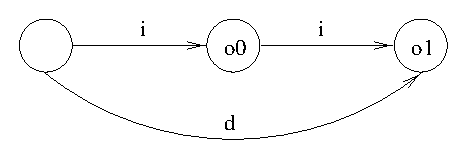
\includegraphics{figures/callfsaeg.eps}}
\centerfigend{fig-callfsaeg}{Sample FSA to Place Integer and Double 
	Floating Point Arguments on Registers}

Given the inadequacy of CCL for out task, we have developed two
new specification languages to support our analysis. The first,
IPL\footnote{\it Keep those acronyms coming!!} (instruction
pattern language) supports the specification of the instruction
sequences from which the caller and callee prologues and epilogues
are composed. IPL is an extension of SLED~\cite{Rams94b}, a language
to support descriptions of machine instruction syntax. IPL extends
SLED to provide support for regular expressions to the language where
the atoms of an expression are individual instructions. The second
language we have developed is PAL (procedure abstraction language).
which provides a means for specifying the calling convention and
other procedure aspects of object code as specified in an ABI.

The following sections demonstrate the use of these
specification languages for the SPARC and Intel platforms. More
detailed descriptions of the languages are given in the \uqbt\ 
source code. 


\section*{SPARC}

The standard stack frame for a single SPARC procedure is composed
of (from low to high addresses) a 16-word area to save the register
window, one word to put the address of a struct/union to return by a
callee, 6 words for a callee to save the first 6 arguments (passed
in registers) to the stack, $n$ words for output arguments 7 and
above, and an area to store locals.  Figure~\ref{fig-stkfrmSparc}
shows the standard stack frame for SPARC.

\centerfigbegin
\resizebox{8cm}{!}{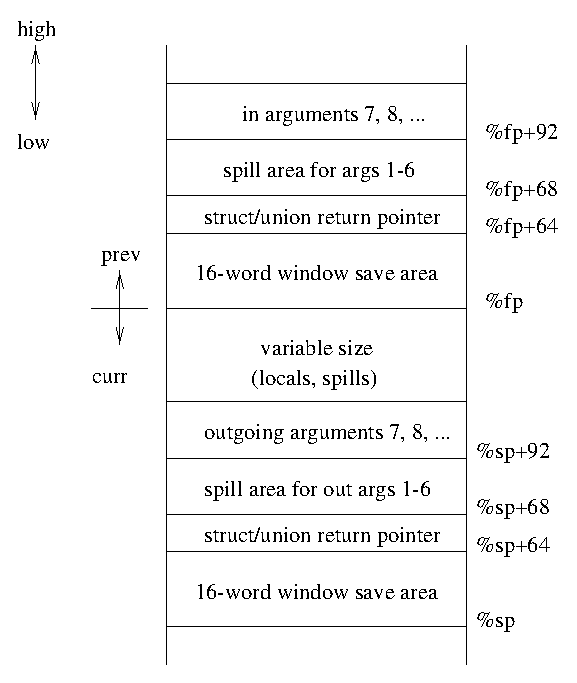
\includegraphics{figures/stkfrm-sparc.eps}}
\centerfigend{fig-stkfrmSparc}{Standard Stack Frame for SPARC Code.
The indexes and register's are given from the context of the callee.}


\subsection{Prologues and Epilogues}

Prior to specifying the prologues and epilogues, it is convenient
to introduce symbolic names for register encodings\footnote{This
is analogous to the {\tt names} construct in SLED.}. For example,
the symbolic name for register 24 on SPARC is {\tt \%o0}. The
set of names defined for SPARC are shown below.

\begin{verbatim}
NAMES
    SP = 14
    FP = 30
    o0 = 8
    i0 = 24
    i7 = 31
    o7 = 15
    g0 = 0
\end{verbatim}

On the SPARC, there are two different ways of invoking a function
based on the return type of the function.  A \texttt{call}
instruction is always used. If the return value is a structure,
union or a quad floating point value, the instruction following the
delayed instruction of the \texttt{call} needs to be a \texttt{unimp}
instruction.  The immediate 22 bits of the \texttt{unimp} are used
to specify the size of the returned value\footnote{Not all compilers
(e.g. gcc) make use of this information to generate runtime size
checking code.}.

\begin{verbatim}
PATTERNS
    CALLER_PROLOGUE std_call addr IS
        call__ (addr)

    CALLER_PROLOGUE struct_call addr IS
        call__ (addr); 
        <4>;  # any 4 byte instruction
        UNIMP (imm22)
\end{verbatim}

The callee prologues that have been identified to date are shown
below. The first two are used when the size of the stack to be
allocated fits into a 13 bit immediate operand. The first one effects
a change to the register window (i.e. allocates a new set of {\it
local} and {\it out} registers) where as the second doesn't. The last
two are analogs of the first two and handle procedures that allocate
a stack whose size cannot be stored in a 13 bit number. A procedure
may not have a prologue at all, as in the case of a leaf procedure
(see page 198 of~\cite{Sparc8}) that doesn't require any stack space.

{\it Note: The last two patterns shown here cannot be used yet as
the pattern parser cannot handle equations or local variables. See
\S\ref{sec:future_work} for a complete description of what is yet
to be implemented to support procedure recovery.}

\begin{verbatim}
    CALLEE_PROLOGUE new_reg_win locals IS
        SAVE ($SP, imode(locals), $SP)

    CALLEE_PROLOGUE same_reg_win locals IS
        ADD ($SP, imode(locals), $SP)

    CALLEE_PROLOGUE new_reg_win_large locals { locals = hiVal+lowVal } IS
        sethi(hiVal,reg);
        ADD (reg, imode(lowVal), reg);
        SAVE ($SP, rmode(reg), $SP)

    CALLEE_PROLOGUE same_reg_win_large locals { locals = hiVal+lowVal } IS
        sethi(hiVal,reg);
        ADD (reg, imode(lowVal), reg);
        SAVE ($SP, rmode(reg), $SP)
\end{verbatim}

The callee epilogue for a procedure on SPARC depends on the following
factors:

\begin{itemize}
\item Does it return an aggregate value?
\item Is it a leaf procedure?
\item Is the value to be returned (if any) already in the right
      location?
\item Has it allocated its own stack?
\end{itemize}

While most combinations of these factors are legal, the majority
of programs will only use a limited subset of the possibile
combinations.  The most common represents a standard return from
a non-leaf procedure (and hence resets the register window). The
value to be returned is already in the expected location ({\tt \%o0}
in this case). The alternatives for the first instruction (i.e. the
actual transfer of control) represent the cases of a scalar (or void)
return value and an aggregate return value respectively.

\begin{verbatim}
    CALLEE_EPILOGUE std_ret IS
        [ ret() |
          JMPL (dispA ($i7, 12), $g0) ];
        restore_()
\end{verbatim}

Two other common combinations are similar to the above except the
value to be returned is moved into the expected location by the
{\tt restore} instruction.

\begin{verbatim}
    CALLEE_EPILOGUE ret_reg_val rs1, rs2 IS
        [ ret() |
          JMPL (dispA ($i7, 12), $g0) ];
        RESTORE (rs1, rmode(rs2), $o0)

    CALLEE_EPILOGUE ret_imm_val rs1, imm IS
        ret();
        RESTORE (rs1, imode(imm), $o0)
\end{verbatim}

Lastly, a leaf procedure usually returns with a {\tt retl}
instruction when returning a void or scalar value or a {\tt jmpl}
instruction when returning an aggregate value. The extra offset from
the calling address in the latter case is to skip the {\tt unimp}
instruction discussed previously.

\begin{verbatim}
    CALLEE_EPILOGUE leaf_ret IS
        [ retl() |
          JMPL (dispA ($o7, 12), $g0) ];
        { SUB ($SP, imode(?), $SP) }
\end{verbatim}

Once the callee returns, any return values are in the right place
and the stack has been restored, so there is no caller epilogue.

The prologues and epilogues presented in this section are the basis
for the PAL specification. The PAL specification encapsulates the
information present in the ABI that describes how parameters are
passed and values returned, where locals are stored and any other
architecture specific information. The following sections present the
sections of the PAL specification for SPARC ABI compliant programs.

\subsection{Frame Abstraction}

To simplify a PAL specification, the first section specifies how to
abstract frame and stack relative address by converting them to be in
terms of a single fixed point, the abstract frame pointer (AFP or
{\tt \%afp}).  Typically, this point should be the value of the stack
pointer after the callee prologue (if any) has been effected as this
is when the abstraction specified takes place. On SPARC, {\tt \%afp}
is indeed initialised to the stack pointer (i.e. {\tt \%sp}). The
substitutions to convert other frame and stack relative addresses to
{\tt \%afp} relative addresses is specified in terms of the callee
prologues previously specified. The only two\footnote{Well four, if
you consider the prologues we can't yet handle.} callee prologues on
SPARC are similar enough that the same substitution for the frame
pointer (i.e. {\tt \%fp}) can be used.  The analysis tracks any
changes to either {\tt \%sp} or {\tt \%fp} throughout the procedure
and updates their respective substitutions correspondingly.

\begin{verbatim}
FRAME ABSTRACTION
    INIT = %sp
    new_reg_win
    same_reg_win
    {
        %fp -> %afp - locals
    }
\end{verbatim}


\subsection{Local Variables}
Local variables are stored within a procedure's stack frame. The size
of this stack frame can be derived from a callee prologue (\textit{We
are assuming that this is always true}). The example below states
that on SPARC, the amount of space (in bytes) allocated for local
variables is equal to the value of the {\tt locals} parameter of
the {\tt new\_reg\_win} and {\tt same\_reg\_win} callee epilogues.

\begin{verbatim}
LOCALS
    new_reg_win
    same_reg_win
    {
        locals
    }
\end{verbatim}

{\it Ideally, we would like to recognise any access addresses within
the portion of the stack frame used for local variables. However,
given the problem of aliasing this is non-trivial and requires
extensive analysis. Even with such analysis, there is no guarantee
that all such references will be detected. The approach we take is
simpler and completely reliable. The user specifies how to derive
the size of the block of memory allocated for locals from the callee
prologue\footnote{I am assuming that this will always be possible}.}

\subsection{Parameter Locations}

As discussed in \S\ref{sec-callConvSpec}, at the machine-code
level we cannot distinguish the variables and types that were used
when placing parameters on appropriate parameter-passing locations.
On SPARC, all parameters are copied by instances of one word, hence,
a double floating point value is copied as two words, in exactly
the same way as two individual integers or even two addresses are
copied.  Low-level type information can be retrieved from usage at
the called site.

The ABI specifies which locations are used for passing parameters,
and the order of usage of those locations. The means by which
the parameters are referenced across a call boundary is dependent
upon the {\it view change} effected by a call. The view change can
be thought of as the low level analog of using actual and formal
parameters in source code. That is, the same parameter is referenced
differently depending on whether the context of the reference is
the call instruction or in the called procedure.

To account for the view change effected by a call, we specify
parameter locations from the both context of the caller (outgoing
parameters) and the callee (incoming parameters).

The first part of the parameters section specifies where the outgoing
parameters are found. This is acheived by attaching a parameters
specification to the {\tt CALLER} keyword.

\begin{verbatim}
PARAMETERS
    CALLER
    {
        AGGREGATE -> m[%afp + 64]
        REGISTERS -> %o0 %o1 %o2 %o3 %o4 %o5
        STACK     -> BASE = [%afp + 92]
                     OFFSET = 4
    }
\end{verbatim}

Each sub-clause is optional but if present, it must obey the
ordering implied in the above example (i.e. {\tt AGGREGATE} before
{\tt REGISTERS} before {\tt STACK}). This ordering complies with
how parameters are passed on all architectures we have encountered.

The \texttt{AGGREGATE} sub-clause states where the address of an
aggregate value to be returned is found. This location will only
be used by calls to procedures that actually return a struct.
Additionally, only some architectures (such as SPARC) make use of
a special location for this purpose. Others (e.g. Intel) simply
pass it as the first parameter\footnote{This effectively makes it a
``hidden" argument in that it doesn't correspond to any source code
level parameter.}.

The {\tt REGISTERS} sub-clause states that registers {\tt \%o0..\%o5}
(in that order) are used for the first 6 parameters (after the
aggregate address parameter if used). Any extra parameters are
passed via the stack and are found in locations {\tt m[\%afp + 92],
m[\%afp + 96], m[\%afp + 100], ...} as specified by the {\tt STACK}
subclause.

In addition, there can be an {\tt ALIGNMENT} sub-clause, after the
{\tt STACK} and before the closing curly bracket. {\tt REGISTERS}
can also have a
type before it, to designate the type of parameters that the given
registers can hold. The type can be one of {\tt INTEGER}, {\tt FLOAT},
or {\tt DOUBLE}. Where a type is not given, as above, {\tt INTEGER} is
assumed. Where more than one type of register is given, they must be
in the order {\tt INTEGER}, {\tt FLOAT}, then {\tt DOUBLE} (with any or
all being optional). For example, for HP pa-risc:

\begin{verbatim}
PARAMETERS
    CALLER
    {
        AGGREGATE -> m[%r28]
        INTEGER REGISTERS -> %r26 %r25 %r24 %r23
        FLOAT   REGISTERS -> %fr4 %fr5 %fr6 %fr7
        DOUBLE  REGISTERS -> %fd5 %fd7
        STACK -> BASE = [%afp - 52]
                 OFFSET = -4
        DOUBLE ALIGNMENT 8 BYTES
    }

\end{verbatim}

When multiple {\tt REGISTERS} are given as above, they are considered to
operate ``in parallel". In other words, when the first parameter goes into
either \%r26 or \%fr4, this ``parameter slot" is ``used up", and so the next
parameter goes into register \%r25, \%fr5, or \%fd7, depending on the type.
If the first parameter is a {\tt DOUBLE}, then two parameter slots are
used up.

The {\tt ALIGNMENT} sub-clause states that parameters of type {\tt DOUBLE}
(64 bit floating point) are aligned on 8 byte boundaries. This applies to
registers and stack locations alike; that's why there are only two
{\tt DOUBLE REGISTERS}. As an example, if a pa-risc function took an
integer, a double, and an integer, then even though these could easily
fit into three registers, they are actually placed in registers \%r26,
\%fd7, and stack location [\%afp-52]. The alignment of the double parameter
``skips" register \%r25, and because doubles are twice as big as integers,
using \%fd7 ``uses up" the parameter slots for \%r24 and \%r23. So the third
parameter has to go to the stack. If there was a fourth parameter of type
{\tt DOUBLE}, it would go to [\%afp-64] (and the other half at [\%afp-60]),
skipping the word at [\%afp-56] to keep the argument aligned on 8 byte
boundaries.

This indicates a significant difference between SPARC and pa-risc architectures.
On the non aligned SPARC, a {\tt DOUBLE} parameter could be split between
an integer register and the stack. On the aligned pa-risc, such splits
can't happen. On the other hand, ``gaps'' in the parameters can be seen
in pa-risc programs, while these will never be seen on the SPARC.

Outgoing parameters are always placed at the same locations. Incoming
parameters however, depend upon the prologue of the procedure being
invoked as it is this prologue that effects the aforementioned
view change. Stack parameters may be found at different offsets
after allocation of the procedure's stack frame. Also, a register
window change will mean that some registers will now accessed via
different register names.

On SPARC, the {\tt new\_reg\_win} prologue changes the register
window, effectively renaming the eight output registers ({\tt
\%o0..\%o7}) to the eight input registers ({\tt \%i0..\%i7}).

\begin{verbatim}
    new_reg_win
    {
        AGGREGATE -> m[%afp - locals + 64]
        REGISTERS -> %i0 %i1 %i2 %i3 %i4 %i5
        STACK     -> BASE = [%afp - locals + 92] 
                     OFFSET = 4
    }
\end{verbatim}

The other prologue, {\tt same\_reg\_win}, doesn't change the register
window but changes the stack offsets.

\begin{verbatim}
	same_reg_win
    {
        AGGREGATE -> m[%afp - locals + 64]
        REGISTERS -> %o0 %o1 %o2 %o3 %o4 %o5
        STACK     -> BASE = [%afp - locals + 92] 
                     OFFSET = 4
    }
\end{verbatim}

\subsection{Return Locations}

Return values need to be placed in specific registers depending on
the type of the value to be returned. As with incoming parameters,
the locations used will depend on the view change effected by the
prologue of the procedure doing the return.

\begin{verbatim}
RETURNS
    ret_reg_val
    ret_imm_val
    leaf_ret
    CALLER
    {
        INTEGER   IN %o0
        ADDRESS   IN %o0
        FLOAT     IN %f0
        DOUBLE    IN %f0to1
    }
    std_ret
    {
        INTEGER   IN %i0
        ADDRESS   IN %i0
        FLOAT     IN %f0
        DOUBLE    IN %f0to1
    }
\end{verbatim}

Note that double refers to a 64 bit float and as such is returned in
a synthetic register that denotes two 32 bit registers.

Once again, the {\tt CALLER} keyword indicates that the accompanying
specification is from a caller's perspective. In this case it is
where a caller will receive a returned value.

\subsection{Accesses to a Parent's Stack}

This is the first (and so far, only) section that is optional in
that not all architectures will require it.

On SPARC, a procedure may write to a certain portion of its parent's
stack frame. This capability is provided primarily so that parameters
in registers can be spilled to the stack resulting in all parameters
being located in a contiguous segment of memory. This is typically
required when the source code uses variable argument lists or
takes the address of a parameter. Compiler writers can leverage
this capability and use this portion of the parent's stack as
space for temporary variables. In order to abstract away from
referring stack locations, we replace accesses to these addresses
with variables. To do so requires that these addresses are specified
in a PAL specification as shown below.

\begin{verbatim}
PARENT STACK
    new_reg_win
    same_reg_win
    {
        %afp - locals + 68 TO %afp - locals + 88 STEP 4
    }
\end{verbatim}

\section*{Intel}

The standard stack frame of a procedure includes space for arguments,
the return address of the caller, the frame pointer value of the
caller (\texttt{\%ebp}), and enough space for local variables and
spilled values (including registers that need to be preserved across
procedure calls).  Figure~\ref{fig-stkfrmIntel} shows the standard
stack frame for Intel code.

\centerfigbegin
\resizebox{10cm}{!}{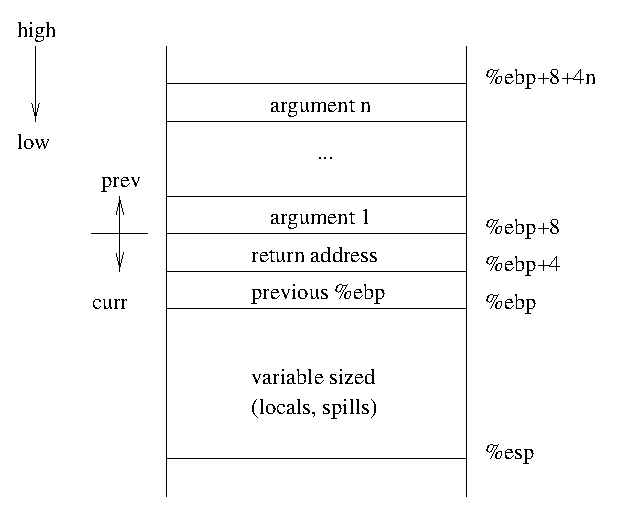
\includegraphics{figures/stkfrm-intel.eps}}
\centerfigend{fig-stkfrmIntel}{Standard Stack Frame for Intel Code}

\subsection{Prologues and Epilogues}

As with SPARC, we start the prologue and epilogue specification by
declaring symbolic names for the register encodings.

\begin{verbatim}
NAMES
    EAX = 0
    ECX = 1
    EDX = 2
    EBX = 3
    ESP = 4
    EBP = 5
    ESI = 6
    EDI = 7
\end{verbatim}

On Intel x86, there is only one way to invoke a procedure, even if
the procedure is to return a value or a structure.  The \texttt{call}
instruction is used, and although this assembly instruction maps to
one of five different machine instructions, only one is used for
direct calls; the intra-segment direct call {\tt CALL\_.JVOD}.  For
indirect calls (i.e. via a register), the intra-segment indirect call
is used (CALL.EVOD modrm).  Indirect calls require extra analysis to
determine the target address of the call; this is addressed in a
different document.  For now assume all calls are direct.

\begin{verbatim}
PATTERNS
    CALLER_PROLOGUE std_call addr IS
        CALL.Jvod (addr)
\end{verbatim}

The most common callee prologue sets up the frame base pointer and
the stack pointer, as well as optionally allocating space on the
stack for locals and spilled values.  Further, the contents of
registers \texttt{\%edi}, \texttt{\%esi} and \texttt{\%ebx} need to
be preserved across procedure calls.  That is, if these registers are
used by the callee, they need to be spilled to the stack as part of
the prologue. 

\begin{verbatim}
    CALLEE_PROLOGUE std_entry locals=0, regs IS
        PUSHod ($EBP);
        MOVrmod ($EBP, Reg($ESP));
        { SUBiodb (Reg ($ESP), locals) |
          SUBid    (Reg ($ESP), locals) };
        { [ PUSHod ($ESI) |
            PUSHod ($EBX) |
            PUSHod ($EDI) ] *regs <1..3> }
\end{verbatim}

In the case where an aggregate value is to be returned, the address
at which this value is to be stored can be passed as the first
(hidden) argument of the call. It has been noted that some compilers
move this address into {\tt \%eax} as part of the prologue\footnote{
Initially this was believed to be an optimisation as the address of a
returned aggregate value must be in {\tt \%eax} upon returning from
the procedure.  However, analysis shows that this is not the case as
these procedures subsequently write to {\tt \%eax} before doing a
return. It does mean the simple form of {\tt RET} can be used in the
epilogue but I'm not sure that this can be classified as an
optimisation}.

\begin{verbatim}
    CALLEE_PROLOGUE struct_ptr locals, regs IS
        POPod ($EAX);
        XCHG.Ev.Gvod (E (Base ($ESP)), $EAX);
        @std_entry (locals, regs)  
\end{verbatim}

The standard epilogue restores any of the registers that need to be
preserved across a procedure call (i.e. \texttt{\%ebx},
\texttt{\%esi} or \texttt{\%edi}), restores the stack pointer and the
frame pointer, and returns to the caller's return address.  Restoring
registers to be preserved across procedure calls can be done in one
of two ways; by popping them from the stack, or by indexing into the
stack directly.  It has also been noticed that some compilers
generate a \texttt{LEAod} (load effective address) at the start of
the epilogue, to ensure the stack pointer is pointing to the right
address, even if this instruction is redundant (as has been seen in
gcc -O2 generated code). The {\tt RET.Iw} instruction is used to
remove the address of a returned aggregate value if this hasn't
already been done so by the prologue.

\begin{verbatim}
    CALLEE_EPILOGUE std_ret IS
        { LEAod ($ESP, Disp8(?,$EBP)) };
        { [ MOVrmod ($EBX, E( Disp8(?,$EBP))) |
            MOVrmod ($ESI, E( Disp8(?,$EBP))) |
            MOVrmod ($EDI, E( Disp8(?,$EBP))) ] * <1..3>
          |
          [ POPod ($EBX) |
            POPod ($ESI) |
            POPod ($EDI) ] *<1..3> };
        [ LEAVE () | [ MOVrmod ($ESP, Reg($EBP)); POPod ($EBP) ]];
        [ RET () | RET.Iw (?) ]
\end{verbatim}

Simple procedures that use no stack and take no parameters have a
very basic epilogue.

\begin{verbatim}
    CALLEE_EPILOGUE simple_ret IS
        RET () | RET.Iw (?)
\end{verbatim}
 

Upon return from a call, the stack needs to be restored by the caller in 
order to remove the parameters that were passed on the stack.  
Restoring of the stack is done by modifying the value of the stack
pointer by a certain number of bytes, or by popping values from the
stack a certain number of times (4 bytes at a time).  Either way 
will tell us how many bytes are restored from the stack. 

\begin{verbatim}
    CALLER_EPILOGUE clear_stack n IS
        [ ADDiodb (Reg($ESP),n) | ADDid (Reg($ESP),n) ] |
        [ POPod ($EAX) |
          POPod ($EBX) |
          POPod ($ECX) |
          POPod ($EDX) |
          POPod ($ESI) |
          POPod ($EDI) |
          POPod ($EBP) ] * n <1..7>
\end{verbatim}

\subsection{Frame Abstraction}

On Intel, we initialise {\tt \%afp} to be the value of {\tt \%esp}
after the prologue (if any) has been executed. As with SPARC, a
similiar substitution is specified for the frame pointer.

\begin{verbatim}
FRAME ABSTRACTION
    INIT = %esp
    std_entry
    struct_ptr
    {
        %ebp -> %afp + (regs * 4) + locals
    }
\end{verbatim}


\subsection{Local Variables}
The size of the block of memory allocated for local variables will
be the initial increment to the stack pointer plus the number of
bytes pushed to the stack when preserving registers.

\begin{verbatim}
LOCALS
    std_entry
    struct_ptr
   {
      locals + (regs * 4)
   }
\end{verbatim}

\subsection{Parameter Locations}

Outgoing parameters on Intel are always found at the bottom of the
stack. Given that we can't statically specify where the bottom of
the stack is, we simply choose a fixed stack address. Accompanied
with a negative offset, this implies that all address that are at
multiples of this offset from are potential parameter locations. The
analysis will then determine which of these locations are live at a
call and recovery as many as it needs to match the signature of the
callee, starting at the lowest addresses. This is exactly the same
approach taken with stack parameters on SPARC but the fixed point
specified in the SPARC PAL specification just happens to be the lowest
address (as implied by the positive offset accompanying it).

\begin{verbatim}
PARAMETERS
    CALLER
    {
        STACK     -> BASE = [%afp - 4]
                     OFFSET = -4
    }
\end{verbatim}

Procedures with the {\tt std\_entry} prologue will find their incoming
parameters at positive offset from the frame pointer. Of course, the
specification is given in terms of {\tt \%afp} as we want to abstract
away from concepts such as a frame pointer.

\begin{verbatim}
    std_entry
    {
        STACK     -> BASE = [%afp + locals + (regs * 4) + 8]
                     OFFSET = 4
    }
\end{verbatim}

The {\tt struct\_ptr} prologue contains the side effect of popping
the address of the aggregate value to be returned from the stack into
{\tt \%eax}\footnote{It it turns out that some other register is used,
then the register used can be parameterised in the pattern and the
parameter name used here instead of {\tt \%eax}.}. As such, the
incoming parameters specification for procedures prefixed with this
prologue require an {\tt AGGREGATE} location to be included.

\begin{verbatim}
    struct_ptr
    {
        AGGREGATE -> %eax
        STACK     -> BASE = [%afp + locals + (regs * 4) + 8]
                     OFFSET = 4
    }
\end{verbatim}

\subsection{Return Locations}

The RETURNS section specifies where returned values can be found. Again,
there are subsections for each callee prologue, and one for callers, using
the special keyword CALLER. Often the different integer values (byte,
short, int) are returned in the same register. If, and only if, the register
numbers are different for the integral subtypes, then an entry should exist
for INTEGER.16 and so on. On a RISC machine like SPARC, parts of registers
are typically not given different register numbers, so these don't appear:

\begin{verbatim}
RETURNS
# Note: even though functions with save/restore return integer locations in %i0,
# we use the STD_RET_ pseudo instruction for these, which copies %i0 to %o0.
# This simulates the semantics of the restore (for the purposes of return
# location), so we don't need a separate set of locations for these functions
    ret_reg_val
    ret_imm_val
    leaf_ret
    std_ret
    CALLER
    {
        INTEGER.32  IN %o0
        ADDRESS     IN %o0
        FLOAT.32    IN %f0
        FLOAT.64    IN %f0to1
    }
\end{verbatim}

On Intel, all fixed point scalar values are returned in {\tt \%eax},
but the word and byte part of eax is called a different register name.
All floating point values are returned on the top of the floating
point stack. The register number of the top of stack depends on whether
a caller or callee is involved:

\begin{verbatim}
RETURNS
    std_ret
    frameless_epi
    {
        INTEGER.32  IN %eax
        INTEGER.16  IN %ax      # So that functions returning shorts
        INTEGER.8   IN %al      # or chars can be analysed as such
        ADDRESS     IN %eax
        FLOAT.80    IN %st7
    }

    CALLER
    {
        INTEGER.32  IN %eax
        INTEGER.16  IN %ax      # So that functions returning shorts
        INTEGER.8   IN %al      # or chars can be analysed as such
        ADDRESS     IN %eax
        FLOAT.80    IN %st
    }
\end{verbatim}

\subsection{Accesses to a Parent's Stack}

Intel procedures never access any stack locations outside of their
own stack apart from those storing incoming parameters.

\section{Procedure Abstraction Analysis}

The goal of this analysis is to use the specification described in the
preceeding sections to remove any references to stack locations in
object code. Such references will be recovered into either parameters
or local variables. There are 5 steps involved in this analysis:

\begin{enumerate}
\item Replace all stack and frame pointer relative addresses with
  their equivalent {\tt \%afp} relative addresses.
\item Recover the signature (parameters only) of user code procedures.
\item Analyse each call to recover the actual parameters of the call.
  this step also includes recovering the return type of the procedure
  called if it isn't a library procedure.
\item Replace any accesses from within a procedure to locations in its
  parent's stack with accesses to local variables.
\end{enumerate}

This analysis is to be performed only on user procedures; library
procedures will be assumed to have been processed by now, either
through generation of call signatures from header files or through
application of the following analysis to library code.

The following subsection consider each of the above steps in
detail. Throughout this section we will make use of the SPARC
example in Figure~\ref{fig-c_gcd}.  Issues specific to Intel are
discussed in $\S$\ref{sec-callsigIntel}.

\centerfigbegin
{\small
\begin{verbatim}
gcd:                           main:
    save %sp,-112,%sp               save %sp,-112,%sp
    mov %i0,%l0                     mov 10,%o0
    cmp %l0,%i1                     mov 5,%o1
    bge .LL12                       sethi %hi(.LLC0),%l0
    mov %i1,%i0                     call gcd  
    b .LL12                         or %l0,%lo(.LLC0),%l0
    mov %l0,%i0                     mov %o0,%o3
.LL6:                               mov %l0,%o0
    call .rem                       mov 10,%o1
    mov %i0,%o1                     call printf  
    cmp %o0,0                       mov 5,%o2
    bne,a .LL12                     ret
    add %i0,-1,%i0                  restore
    mov %i1,%o0
    call .rem  
    mov %i0,%o1
    cmp %o0,0
    be .LL10
    nop
    add %i0,-1,%i0
.LL12:
    cmp %i0,1
    bg .LL6
    mov %l0,%o0
.LL10:
    ret
    restore
.LLC0:
    "gcd of %d, %d is %d\n"
\end{verbatim}
}
\centerfigend{fig-c_gcd}{SPARC Assembly Code for GCD Program}


\subsection{Recovery of Parameters}
Actual parameters are placed by the caller in one or more of the
locations specified by \texttt{caller parameters}.  The callee
will effect the \texttt{view change} applicable to its prologue, 
and will then use the passed parameters directly or place them 
on the parameter spill area.  Either way, the parameters are 
used before definition within the callee, and this is what 
tells us that the information in that location was setup elsewhere
in the program. 

In the example of Figure~\ref{fig-c_gcd}, \texttt{main} calls 
\texttt{gcd}, using the most frequently used calling convention;  
\texttt{interface1}.  
At the \texttt{call} site, the parameter locations that are live are: 
\begin{verbatim}
     live = {%o0, %o1}
\end{verbatim}
At the callee site, we apply the \texttt{view change} of 
\texttt{callee\_prologue1} to the live parameter locations, the 
stack pointer, and the return address, leading to
\begin{verbatim}
     %o0 -> %i0
     %o1 -> %i1
     %sp -> %fp
     %o7 -> %i7
     %sp -> %sp-112
\end{verbatim}
For \texttt{gcd} we summarize the live-in information for the whole 
procedure based on the parameter locations (view changed).  This gives us
\begin{verbatim}
     liveIn(gcd) = {%i0, %i1}
\end{verbatim}
This information tells us that there are 2 parameters, which match the
two live parameter locations at the call site, hence the actual 
parameters to the call are \texttt{\%o0} and \texttt{\%o1}.  The 
transformed CALL instruction looks like this:
\begin{verbatim}
     CALL gcd [<ret type>] <(%o0,<type>), (%o1,<type>)>
\end{verbatim}

Note that for parameter locations that are on the stack, the 
view change of these looks as follows:
\begin{verbatim}
     %sp+92+n -> %fp+92+n
\end{verbatim}
Hence, accesses to \texttt{\%fp+92+n} at the callee site are 
accesses to parameter locations.  It is also feasible for the
callee site to access these locations using the stack pointer; 
this is needed for leaf routines but it can also be used in 
non-leaf routines: 
\begin{verbatim}
     %sp+(92+simm13)+n
\end{verbatim}
We need to support both views of stack parameter locations.


\subsubsection*{Fixed vs Variable Number of Arguments}
Most procedures take a fixed number of arguments.  However, languages
like C allow for variable number of arguments to be passed at any
one time.  The ABI~\cite{Unix90} does not place any rules on variable 
number of parameters, but states that the calling convention rules need to 
be satisfied; that is, the first 6 word parameters go into registers
and the next go onto the stack.  Disassembled C code shows that 
the first thing the callee does is to move all the register parameters
to the parameter spill area, and then use them all on the stack 
(as the stack parameters are contiguous to the spilled register 
parameters). 

It is not clear that in all cases usage analysis of parameter 
locations at the callee will determine the number of parameters
taken by the callee (think of \texttt{printf}, it can take any
number and the code is bound to be a loop on a string).  
Also, different invocations of the procedure will take different
number of arguments.
\emph{I propose we pass all the live parameter locations at the call
site in the mean time; we will see from the implementation whether
this will cause problems with stack parameter locations.}


\subsection{Recovery of Return Value}
The callee will place a return value on a valid \texttt{callee return}
location.  We note that if anything is placed on a return location,
this location will be live-out of the callee.  
The caller will need to apply the inverse of the \texttt{view change}
to live-out callee locations.  
If the caller is to make any use of a returned value, the location
where it was stored will be used before being re-defined.  Usage is 
commonly in the form of storing to a local variable or using it
as a parameter to another procedure.  
Once this is determined, the callee's RET instruction is set to 
return the relevant return location.
 
For the example of Figure~\ref{fig-c_gcd}, the callee, \texttt{gcd}, 
has only one return location live-out, which matches its \texttt{callee
return} for \texttt{interface1}: 
\begin{verbatim}
     live-out = {%i0}
\end{verbatim}
The caller uses \texttt{\%o0} before definition, hence this is our
return location. 
The callee's RET instruction can now be transformed to: 
\begin{verbatim}
    RET %i0
\end{verbatim}
The caller's CALL instruction can now be transformed into an ASSIGN 
(assignment) instruction as follows: 
\begin{verbatim}
    %o0 = CALL gcd <(%o0,<type>), (%o1,<type>)>
\end{verbatim}

\emph{Should we introduce a HL ASSIGN or shall we use RTL assign 
instead?}

Note that as of 8th September 2000, the return value analysis is done before
the actual parameter analysis. This is because the return value analysis
may cause re-analysis of some of the children, which may impact on the
parameters of the call being considered.

\subsubsection*{Returned Values not Used}
Returned function values are not always used by the caller.  In such
cases, different invocations of the same procedure will show different
return location usage.  In these cases, we go for the more general 
one (i.e. the procedure returns a value) and we annotate each actual 
call with whether the return value is used or not.  In this way, the
signature for the procedure is correct. 


\subsection{Issues Relating to Intel Call Signature Analysis}
\label{sec-callsigIntel}
The nature of Intel passing parameters on the stack means that
optimizing compilers may delay the restoring of the stack until 
after several calls to (different) procedures have been emitted. 
This means that the caller epilogue is optional, and where 
available, it may not necessarily match the number of bytes 
passed as parameters to the caller but may also include bytes
used in a previous call.  We can still make use of liveness 
analysis to determine which arguments are passed to each procedure 
nevertheless.
For the purposes of illustration, we will make use of 
Figure~\ref{fig-gcdIntel}, an optimized version of the GCD program for Intel.

\centerfigbegin
{\small
\begin{verbatim}
gcd:                        main:
    pushl %ebp                  pushl %ebp
    movl %esp,%ebp              movl %esp,%ebp
    pushl %edi                  pushl %esi
    pushl %esi                  pushl %ebx
    pushl %ebx                  movl $10,%esi
    movl 8(%ebp),%ebx           movl $5,%ebx
    movl 12(%ebp),%edi          pushl %ebx
    movl %edi,%esi              pushl %esi
    cmpl %edi,%ebx              call gcd
    jge .L12                    pushl %eax
    movl %ebx,%edi              pushl %ebx
    jmp .L12                    pushl %esi
.L6:                            pushl $.LC0
    movl %ebx,%eax              call printf
    cltd                        leal -8(%ebp),%esp
    idivl %edi                  popl %ebx
    testl %edx,%edx             popl %esi
    jne .L7                     leave
    movl %esi,%eax              ret
    cltd
    idivl %edi
    testl %edx,%edx
    je .L13
.L7:
    decl %edi
.L12:
    cmpl $1,%edi
    jg .L6
.L13:
    movl %edi,%eax
    leal -12(%ebp),%esp
    popl %ebx
    popl %esi
    popl %edi
    leave
    ret  
.LC0:
    "gcd of %d, %d is %d\n"
\end{verbatim}
}
\centerfigend{fig-gcdIntel}{Intel Optimized Assembly Code for GCD Program}

Procedure \texttt{main} calls \texttt{gcd} using the calling convention 
specified in \texttt{interface2} with an immediate value of 12 bytes. 
The calling convention does not include a caller epilogue. 
At the \texttt{call} site, the \emph{parameter locations} that are live are: 
\begin{verbatim}
     live = {[%esp], [%esp+4]}
\end{verbatim}
Applying the \texttt{view change} for \texttt{interface2} to the live
parameter locations we get: 
\begin{verbatim}
     ['%esp]   -> [%esp+20]
     ['%esp+4] -> [%esp+24]
and
     ['%esp]   -> [%ebp+8]
     ['%esp+4] -> [%ebp+12]
\end{verbatim}
Procedure \texttt{gcd} has the following set of parameter locations
live on entry, and return locations live on exit: 
\begin{verbatim}
     liveIn = {[%ebp+8], [%ebp+12]}
     liveOut = {%eax}
\end{verbatim}
The liveIn parameters match the ones that were live on entry, hence 
we can safely assume that 2 words (8 bytes) were passed as arguments.
The call is transformed to the following HL instruction: 
\begin{verbatim}
    CALL gcd [<ret type>] <([%esp],<type>), ([%esp+4],<type>)>
\end{verbatim}
which is further transformed into what was actually placed at those 
stack locations (i.e. this information needs to be stored previously): 
\begin{verbatim}
    CALL gcd [<ret type>] <(%esi,<type>), (%ebx,<type>)>
\end{verbatim}
The liveOut information tells us that \texttt{\%eax} is returned. 
Further, at the caller's site, the value of \texttt{\%eax} is 
used prior to definition.  Even if this value was not used, the ABI 
states that return locations should only be set to a value if they
are intended to return a value, as there is no type checking on 
this interface.  The return instruction in \texttt{gcd} is changed to
\begin{verbatim}
     RET %eax
\end{verbatim}
and the caller's site call is changed to 
\begin{verbatim}
     %eax = CALL gcd <(%esi,<type>), (%ebx,<type>)>
\end{verbatim} 
Although there is no caller epilogue to restore the stack, we have
determined the right arguments to this call.

The next call that \texttt{main} performs is to the library procedure 
\texttt{printf}.  In this case, if we had signatures for \texttt{printf} 
we could only be assured of one fixed parameter (an address) and maybe
some more parameters, as this is a variable argument procedure.  
Also, the calling convention does not specify a caller epilogue in 
this case either, hence we cannot determine exactly how many bytes
are passed on the stack to this call.  The best that can be done is
to pass \emph{all} parameter locations that are live at the call site: 
\begin{verbatim}
     live = {[%esp], [%esp+4], [%esp+8], [%esp+12], [%esp+16], [%esp+20]}
\end{verbatim} 
When replacing this information into the HL call, we get: 
\begin{verbatim}
     CALL printf <(.LC0,<addr>), (%esi,<type>), (%ebx,<type>), (%eax,<type>),
                  (%esi,<type>), (%ebx,<type>)>
\end{verbatim}
Note that in this case, the last two arguments are still technically
live as the stack wasn't restored.  Although we are passing them to 
\texttt{printf}, the code within \texttt{printf} will not use them 
as they were not expected (by checking the string \texttt{.LC0}). 

If however the stack was restored after the call to \texttt{printf}, 
the following code could have been emitted to restore both calls made
by \texttt{main}: 
\begin{verbatim}
     addl $24, %esp
\end{verbatim}
Which would account for 8 bytes that we already know \texttt{gcd} takes
as arguments, and 16 bytes for \texttt{printf}.  This type of arithmetics
will allow us to determine the number of bytes passed to variable 
argument procedures in some cases (bearing in mind that each time 
a different number of arguments may be passed). 


\section{EBNF for the PAL Language}

The EBNF for the PAL language follows.  The standard EBNF
metasymbols are used:

\begin{itemize}
\item \verb!{a b}! for sequence
\item \texttt{[a]} for optional constructs
\item \texttt{(a|b)} for alternative choices
\item \texttt{*} for zero or more occurrences
\item \texttt{+} for one or more occurrences
\end{itemize}

\begin{fnverbatim}
PALSpec ::= register_names
      caller_prologue_section callee_prologue_section
      callee_epilogue_section [ caller_epilogue_section ]
      frame_section local_section parameter_section
      return_section [ parent_section ]

register_names ::= "NAMES" { name '=' number } +

caller_prologue_section ::=
      "CALLER_PROLOGUE" pro_epi_decl +
callee_prologue_section ::=
      "CALLEE_PROLOGUE" pro_epi_decl +
callee_epilogue_section ::=
      "CALLEE_EPILOGUE" pro_epi_decl +
caller_epilogue_section ::=
      "CALLER_EPILOGUE" pro_epi_decl +
pro_epi_decl ::= constructor_list

frame_section ::= "FRAME ABSTRACTION" init_decl
      frame_decl +
init_decl ::= "INIT" reg_name
frame_decl ::= name + '{' reg_name "->" afp_exp '}'

local_section ::= "LOCALS" local_decl +
local_decl ::= names '{' exp '}'

parameter_section ::= "PARAMETERS" param_decl+
param_decl ::= names
      '{' "AGGREGATE ->" "m[" afp_exp ']'
          "REGISTERS ->" reg_name +
          "STACK -> BASE = [" afp_exp ']'
                   "OFFSET =" number '}'

return_section ::= "RETURNS" return_decl +
return_decl ::= names
      '{' "INTEGER IN " reg_name
          "ADDRESS IN" reg_name
          "FLOAT IN" reg_name
          "DOUBLE IN" reg_name '}'

parent_section ::= "PARENT STACK" parent_decl
parent_decl ::= name + '{' afp_exp "TO" afp_exp
      "STEP" number '}'

operands ::= name { "," name } *
constructor ::= name { '(' operands ')' }
constructor_list ::= constructor
      | constructor ';' constructor_list
exp ::= "(" exp ")"
      | exp "+" exp | exp "-" exp
      | exp "*" exp | exp "/" exp
      | reg_id | number | name
afp_exp ::=
      "%afp +" exp | "%afp -" exp
reg_name ::= name | reg_id

names  ::= ( name | "CALLER" ) +
name   ::= [A-Z][A-Z0-9_]*[A-Z0-9]
number ::= [0-9]*
reg_id ::= '%'[A-Za-z][A-Za-z0-9]*
\end{fnverbatim}


\section{Location Sets}

Many of the analyses described in this chapter rely on sets of bits representing
locations. This section gives an overview of the LocationMap and BitSet classes
which implement these.

\subsection{LocationMap class}

There is one LocationMap object (part of the CSR class) for the whole program.
It represents a mapping from the integers to locations of interest to the
translation. For example, in one translation, integer 0 might represent "r[8]",
and in another translation it could represent "m[\%afp+92]". It is convenient
to define sets of bits to represent sets of locations. In these sets, if
but {\it n} is on, that means that the expression represented by integer {\it n}
is in the set. That way, expressions such as

  $live_{in}~ = ~\stackrel{\bigcup}{_{all BBs}} ~UsedUndefined~ \bigcap
  ~~({\rm U} - live_{in}$)

can be implemented in code such as

    {\tt for (}{\it bb = each in-edge}{\tt )} \\
    \indent {\tt liveIn |= bb->useUndefSet \& \~~(bb->liveIn);}

\subsection{BitSet class}

There is a Standard Template Library (STL) template class called
\texttt{bitset}, which implements a fixed-size array of bits. Unfortunately,
since we don't know in advance how many locations a program may have, we want a
class with the same functionality as \texttt{bitset}, but has a variable size
(like a vector of bits).  The \texttt{BitSet} class implements this
functionality, using a \texttt{vector} of unsigned integers to hold 32 bits
at a time. Standard bitwise operators like \& and $|$ are used to implement
set intersection and union respectively.

Objects of class \texttt{BitSet} have a member variable called \texttt{usedBits}
which stores the number of bits in this set.
Bits are numbered from 0 to \texttt{usedBits-1}.
\texttt{BitSet}s sometimes have to represent the universal set.
To do this properly, there is a boolean class member called \texttt{universal},
which represents the bits numbered from \texttt{usedBits} to infinity.
Normally, \texttt{universal} is zero, so that the set is finite, and bits
not stored in the vector are considered zero. However, the member function
\texttt{set()} (the one taking no arguments) sets the single vector element
to all ones, and sets the \texttt{universal} bit as well. All bits of this
set are considered to be one.

It is important to take the \texttt{universal} bit into consideration when
performing operations such as \texttt{operator\&}, \texttt{set({\it n})},
and so on. Two member functions, both with the name \texttt{setUsed},
expand the vector when required (e.g. setting or clearing a bit higher than can
be represented with the vector at its current size, or \texttt{and}ing or
\texttt{or}ing with a bitset larger than can be represented with the vector
at its current size. When the vector is expanded, the newly inserted words
are either set to all zeroes or all ones, depending on the state of the
\texttt{universal} bit.

Extra care must be taken when \texttt{and}ing or
\texttt{or}ing with a set smaller (in terms of vector size) than the current
set. For example, when \texttt{and}ing with a smaller set, those elements of
the vector beyond the size of other operand's vector are effectively being
\texttt{and}ed with a virtual word whose bits are all set to the other
operand's \texttt{universal} bit. Hence these words are cleared if the other
operand's \texttt{universal} bit is zero, or left the same otherwise.


\section{Future Work for Procedure Abstraction Recovery}
\label{sec:future_work}

This section details possible extensions and enhancements that can be
made to the procedural abstraction module within UQBT (Doug, Sep 99).

\subsection{Pattern Language for Prologues and Epilogues}

The proposals in this section include extensions to the pattern
language itself (IPL), improvements to the corresponding parser
and suggestions to enforce constraints on how the patterns are used.

\begin{itemize}
\item Add support for locals. Locals are variables that are not
  parameters and as such don't require definition before use. Locals
  can be used to constrain operands over a number of instructions
  without requiring that a parameter is used. Also can be used in
  equations. The example below from SPARC displays both uses:

\begin{verbatim}
    CALLEE_PROLOGUE new_reg_win_large locals { locals = hiVal+lowVal } IS
        sethi(hiVal,reg);
        ADD (reg, imode(lowVal), reg);
        SAVE ($SP, rmode(reg), $SP)
\end{verbatim}

  In this example, {\tt hiVal}, {\tt lowVal} and {\tt reg} are
  all local variables. The first two are used in the equation
  to set the value of the {\tt locals} parameter. The {\tt reg}
  variable enforces the operands of the same name in each of the
  three instructions to have exactly the same value for the whole
  pattern to be successfully matched.

\item Add support for equations. This enables pattern definitions
  like the one above where the value of an operand is derived from an
  expression involving operands of the constituent instructions. In
  this form, equations are exactly the same as supported by SLED.
  However it may be desirable to given equations a finer grained
  scope than the whole instruction. This would allow pattern
  definitions such as the one below where the value of a parameter
  is derived or explicit depending on which branch of the matching
  expression was taken.

\begin{verbatim}
    CALLEE_PROLOGUE new_reg_win locals IS
        SAVE ($SP, imode(locals), $SP) |
        [ sethi(hiVal,reg);
          ADD (reg, imode(lowVal), reg);
          SAVE ($SP, rmode(reg), $SP)
          { locals = hiVal + lowVal }
        ]
\end{verbatim}

  The primary advantage of this extension is that one epilogue
  can match a greater variety of patterns. However it comes at
  the disadvantage of added complex to both the language and the
  underlying parser. As it is, the parser will have to extend its
  semantic checking for equations to ensure for example that any
  variables used in the right hand side of an assignment are defined
  on every branch of the matching expression (e.g. lowVal and hiVal)

\end{itemize}


\subsection{Local Variables}
The current local variable section in a PAL spec only supports
specification of the size of the stack frame which in turn is
the amount of memory we allocate for local variables. On some
architectures such as SPARC, the stack frame includes space for
other purposes than just storing local variables such as space
for saving the register window in the case of a register window
overflow. We would like to be able to allow the user to
specify the portion of the stack frame that is dedicated to local
variables. One means of doing so is to specify a base address and a
size (similar to a stack parameter specification) as in the following
example for SPARC:

\begin{verbatim}
    LOCALS
        new_reg_win
        same_reg_win
        {
                BASE = %afp
                SIZE = locals
        }
\end{verbatim}

This example says that the locals parameters are located in the
inclusive range {\tt m[\%afp] .. m[\%afp + locals]}. Using such a
specification ensures that the translated program will only allocate
as much space for locals as was allocated in the source program.

{\it As long as only the size of the stack is specified, the local will
always be indexed at offsets from {\tt \%afp}. For this reason, the
size specified must always be the same as the difference between the
frame pointer and its equivalent {\tt \%afp} relative value. This can
be seen to hold in both the SPARC and Intel PAL specs.}


\subsection{Aggregate Types as Parameter and Return Types}
When analysing calls to user code procedures, both the caller
and callee can be coerced into a form that will guarantee the
successful compilation of the generated intermediate C code on
the target platform. This results primarily from the fact that the
underlying exposes the calling convention for passing and return
aggregate values in the intermediate code.

Library procedures that have aggregate types in their signature will
expect the calling convention on the target platform for passing
and returning these types to be used by calls to them. The only
way we can do this in C code is to typecast the blocks of memory
storing the relevant aggregate values. Consider a call to the
library function with the following signature:

\begin{verbatim}
    time_t time(time_t *t);
\end{verbatim}

To ensure that the code generated by a call to this function
will be ABI compliant with the library on the target platform, the
intermediate C code must use the {\tt time\_t} name as follows:

\begin{verbatim}
    (*(time_t*)(_t) = time(_t);
\end{verbatim}

where {\tt \_t} is a pointer to the block of memory that will store
the {\tt time\_t} struct. There is no need to typecast the parameter
to the call as type clashes between pointer types will result in
compiler warnings but the correct code will be generated. A typecast 
would have been necessary for the parameter if it was not a pointer type.

At the moment, the analysis does not have access to the type names
required for doing the typecasting described above.

\subsection{Implementation}

This sections describes what is left to be done in the implementation
is general apart from the changes suggested in the preceeding
sections.

\begin{itemize}
\item Change all "csr" substring "pal" to reflect that CSR module is
now the PAL module. This includes changes to directory names, files
names, class names, variables name comments etc.
\end{itemize}

         % procedure abstraction recovery

 	%
% 25 Oct 01 - Brian: Added description of endianness analysis during
%              type analysis.
%

\chapter{Type Recovery Analysis}
\label{ch-type}

\newtheorem{typerule}{Type Rule}[chapter]

{\small
\begin{flushright}
Design: Cristina [Mar 99], Implementation: Mike Van Emmerik[c.00], Bernard Wong [Aug 01], Documentation: Cristina [99], Bernard [Aug 01], Brian [Oct 01]
\end{flushright}
}

{\em The bulk of this document was written in 1999 and has not 
been updated much since.  In summer 2001, Bernard implemented some 
of the type propagation ideas presented in this chapter, 
however, the implementation is not fully tested at the 
time of release of this code.} 

Low-level type recovery is the process of recoverying types 
that are available at the machine level in order for 
translated programs to be correct.  
Type recovery is done in a series of steps, by first annotating
locations with their plausible type and then propagating 
types across live ranges of locations.  

This document will grow as we learn more about the type 
requirements for translated programs.  The following are 
the issues that will be addressed throughout this process: 
\begin{itemize}
\item What is the minimal set of low-level types required?
\item How do we best propagate information across procedures?
\item What information do we need to store for byte swapping 
	to work correctly across different endianness machines?
\end{itemize}

In reality, we are mainly interested in determining the low-level 
types for parameters and return values, however, in order to 
do that, one needs to also know the types for other locations 
that define the variables that get passed as parameters. 
This analysis will be done in the following stages: 
\begin{itemize}
\item Recovery of types for registers
\item Recovery of types for local and parameter locations that 
	are not registers 
\item Recovery of types for other memory locations
\end{itemize}

The second stage involves extending the register analysis to 
support local variable locations as well as parameter locations. 
It may be that parameter locations are trivially supported by
the register analysis (once parameters have been determined), 
and so this stage would be involved with the support of 
local procedure memory.

The last stage is an optional one and is there in case we end 
up doing endianness analysis and attempt to minimize the number
of swaps to memory.  

Unless otherwise seen to be needed later, we will work with 
four base low-level types: integer, float, address to data 
and address to instruction.  
Given that the ABI~\cite{Unix90} states that floats and 
integers (of any size) are passed on integer registers, and the  
fact that addresses are also integer numbers, our default data type
for any location is an integer (i.e. the bottom of the lattice).  
In a lattice representation, if a condition holds true, a type can 
be promoted to one higher up the lattice.  In our case, we have a 
few types which can be represented in a very simple lattice as per 
Figure~\ref{fig-typeLattice}. 

\centerfigbegin
%\resizebox{6cm}{!}
{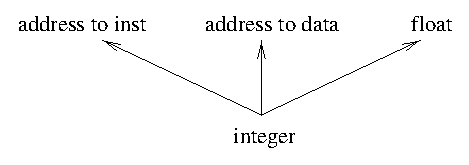
\includegraphics{figures/typeLattice.eps}}
\centerfigend{fig-typeLattice}{Lattice of Low-Level Types} 

Types are determined based on usage of a location across a live
range.  Given that a particular location can be re-used as 
different variables of different types by a compiler, the only
safe assumption is that the live range for a given location will 
have \emph{one} type.  {\emph{I believe this assumption is 
valid for non-overlapping registers.}} 

For the promotion of types, we use a slightly different lattice
to the one displayed in Figure~\ref{fig-typeLattice}.  Distinguishing
integers from addresses is a hard to solve problem as the assembly 
of the machine does not provide for mnemonic instructions to 
distinguish them.  For example, the following code: 
\begin{verbatim}
    sethi %hi(71167),%o1
    or %o1,%lo(71167),%o0
\end{verbatim}
sets register \texttt{\%o0} to the value of \texttt{71167}.  From 
looking at this code alone we cannot tell whether 71167 represents
an address (in the instruction or data area) or a large constant 
number.  Only usage of register \texttt{\%o0} will determine 
the type of 71167.  
For this reason we use the lattice in Figure~\ref{fig-promotionLattice} 
to describe the types of addresses; namely, an integer may ``look like'' 
and address, but until we can identify usage of that integer or 
address, we cannot determine whether it is an address (and hence 
promote to type address). 

\centerfigbegin
\resizebox{6cm}{!}{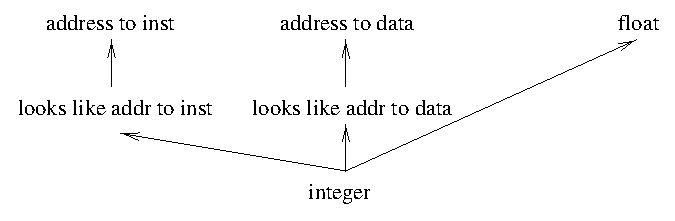
\includegraphics{figures/promotionLattice.eps}}
\centerfigend{fig-promotionLattice}{Lattice of Low-Level Types}

Once a type is determined, types are propagated across the live range 
of the particular location.

Note that even though we place data at the same memory locations
in the target address space as in the source address space, we 
still need to collect type information on pointers to data, as 
this information is needed in getting byte swapping (i.e. the 
simple endianness solution) to work correctly on translated 
programs.


\section{Type Analysis for Registers}
By default, a register is considered to be an integer 
register.  Usage of a register on a procedure call or 
as the return value of a call can change its type.  
Types are propagated from usage to definitions, so here are 
the steps to follow at different parts of the translation 
process: 

\begin{itemize}
\item Collect plausible type information at decoding time.
\item Perform type propagation by type induction.
\end{itemize}


\subsection{Collecting Type Information at Decode Time}
There are three rules that can be used at decoding time 
to annotate type information in registers.  

The first two rules deal with static checking of literal 
constants against addresses of text and data sections, and 
annotating the relevant register to ``looks like'' an address, 
denoted, ``\verb!~!pi'' for looks like a pointer to an instruction, 
and ``\verb!~!pd'' for looks like a pointer to data.  

\begin{typerule}
If a M$_S$-RTL instruction is of the form ``r = Num'' and 
$Num \in$ addrRanges(textSegments), then type(r) = \verb!~!pi.
\label{rule-llpi}
\end{typerule}

\begin{typerule}
If a M$_S$-RTL instruction is of the form ``r = Num'' and 
$Num \in$ addrRanges(dataSegments), then type(r) = \verb!~!pd.
\label{rule-llpd}
\end{typerule}

The following rule applies to any control transfer instruction, 
namely, calls, conditional and unconditional jumps. 
If the target address of the control transfer instruction is 
stored in a register, than that register has pointer to 
instruction type, denoted ``pi''. 

\begin{typerule}
If an M$_S$-RTL instruction is of the form ``controlTransfer r'', then 
type(r) = pi. 
\label{rule-pi}
\end{typerule}


\subsection{Determining Live Ranges of Registers}
In order to propagate types across registers and across 
procedures, live ranges for each register need to be found
first.  A register may take several different variables 
throughout the lifetime of a procedure, hence the need for 
such live ranges. 

A live range extends between the definition (i.e. assignment)
of a register until the death (i.e. re-assignment) of that register.
For example, in the following \texttt{main} code:
\begin{verbatim}
2    mov 10,%o0
3    mov 5,%o1
4    sethi %hi(.LLC0),%l0
5    call gcd
6    or %l0,%lo(.LLC0),%l0
7    mov %o0,%o3
8    mov %l0,%o0
9    mov 10,%o1
10   call printf
11   mov 5,%o2
12   ret
\end{verbatim}

The live ranges for register \texttt{\%o0} are: 
\begin{itemize}
\item Register \texttt{\%o0} becomes live at instruction 2,
    and its live range extends to instruction 5
\item instructions 5 to 8
\item instructions 8 to 10
\item instructions 10 to 12
\end{itemize}


\subsection{Propagating Type Information}
Type propagation can only be performed in \hrtl\ code, i.e. 
after parameter analysis recovery has been performed and 
the program's code has been lifted to the level of machine 
independent RTLs. 

Known types (i.e. non integer) are propagated across live 
ranges of registers, including across procedure calls, 
taking into consideration the signatures for library 
functions.

The first rule states how to go up the lattice when the type 
of the RHS is non integer, basically, propagate from the type of 
the usage to the type of the definition.

\begin{typerule}
If a \hrtl\ instruction is of the form ``r = exp'' and type(exp) = A 
and type(r) = int, then type(r) = A. 
\label{rule-prop-usageDef}
\end{typerule}
 
Note that the type of an expression is the type further up the
lattice of the individual registers forming the expression. 

The next rule looks at the return value of a function call 
and propagates that type to the newly defined register. 

\begin{typerule}
If a \hrtl\ instruction is of the form ``r = call X'' and 
returnType(X) = A, then type(r) = A. 
\label{rule-prop-retValue}
\end{typerule}

The next rule states that a library function's formal argument 
types are propagated to the associated actual parameters.  
In the case of variable argument functions, only the fixed 
formal parameter types can be propagated. 

\begin{typerule}
If a \hrtl\ instruction is of the form ``call libFunc(..., $r_i$, ...)'' 
and the function libFunc has the signature ``libFunc(..., $f_i$=$t_i$, ...), 
then type($r_i$) = $t_i$.  
\label{rule-prop-libFunc}
\end{typerule}
 
The above three rules can be applied on a pass through the code, 
without need of any extra data structures other than the live 
ranges for registers.  The next rule requires extra analysis to 
be performed on procedures, as a register that appears as 
pointing to an instruction may actually be invoked elsewhere in
the program, such as in the \texttt{qsort} program.  

\begin{typerule}
If there is an instruction of the form ``call r''and $\exists$ r2: 
type(r2) = \verb!~! pi, then, if r2 \ra* r, type(r2) = pi. 
\label{rule-reach}
\end{typerule}

In order to apply type rule~\ref{rule-reach}, we need to compute
the reaching definitions of $r2$ throughout the program, including
its transitive closure as the register could have been passed 
as parameter and then copied to another register before it is 
invoked. 


\section{Type Analysis for Other Memory Locations}
Type analysis of other memory locations
can be done to support endianness analysis:
the identification of when endianness swaps are necessary
when the target machine has a different endianness than the source machine.
A translated program's initialized memory is left as-is,
in the source machine's endianness.
We currently swap the bytes of \emph{every} multibyte value
that is read or written to memory.
If type analysis were extended
to include information about the endianness of each value,
then we could determine not only which endianness swaps are unnecessary,
but also when they must \emph{not} be done.
For example, the procedure \texttt{scanf}
is passed an address where its result must be stored.
The value that will be stored in memory
will be in native (target) endianness.
However, when the caller reads the value,
if its bytes are swapped, the native value will be corrupted.
This problem occurs today with every ``call-by-reference'' procedure
that takes addresses where their results are written.

We could do a data flow analysis to discover what values
have native endianness and what do not.
This could be done during type analysis
and a bit set indicating the endianness of each value and location.

Note that it is not enough to specify ``call-by-reference'' information
for just library procedures such as \texttt{scanf}.
The translated program's own procedures
may also be ``call-by-reference''. 


\section{Speculative Decoding}
Trees of program code can be built through speculative 
decoding, in such a way that a forest of trees is built, 
with the main tree being the one that starts at the 
program's entry point.  
Speculative decoding is useful if code ever gets code 
through the interpreter, in which case, the interpreter's 
switch manager can determine if the target address has
already been decoded, in which case, efficient translated
code is run instead of being interpreted.  However, 
speculative decoding is expensive on time resources, 
but for static translators this may be ok anyway.  
 
Type rule~\ref{rule-prologue} states that for all word-aligned
values of $N$ that belong to any of the text segments, if 
the first bytes of that address match a callee prologue (see  
Chapter~\ref{ch-call}, \S\ref{sec-callConvSpec} for SPARC and Pentium 
callee prologues), then $N$ is the start address of a new 
code tree.  

\begin{typerule}
$\forall N: N$ is word-aligned and $N \in addrRanges(textSegments)$ 
and $m[N] \ldots m[N+i]$ = callee\_prologue then type($L$) = $pi$.
\label{rule-prologue}
\end{typerule}

Clearly, applying this technique would be done after the 
normal decoding process and \uqbt\ should have tagged which 
word-aligned memory locations have already been processed 
so that those locations are ignored in this lengthy pass. 


\iffalse
\section{Promotion to Address to Data}
Addresses to data point to data locations in the program, such as
constant data (for example, strings that appeared in the original 
program), and global read and write data. 

An address is an integral number that happens to be a virtual address 
within the range of addresses of the data segment(s) of the program or of 
a symbolic name. 
In Elf binary-files, there are several sections that contain data; 
these are: 
\begin{itemize}
\item Sections that contain read-only data: .rodata, .rodata1
\item Sections that contain initialized read-write data: .data, .data1
\item Section of uninitialized read-write data: .bss
\end{itemize}
Each of these sections has identifying information to know the 
section name, its virtual address and its size.
This data provides us with information that can be used in 
determining whether an integer is an address to data or not. 

The following rules are used to promote integers to addresses to data.
We denote ``address to data'' by $addr_d$ and ``looks like address to 
data'' as $ll_{addr_d}$. 

\begin{typerule}
If $m[i]$ then type(i) = $addr_d$
\label{rule-index}
\end{typerule}

Type rule \ref{rule-index} states that any memory access implies an address 
through its index.  This will be the case for both load and store 
instructions.  Further, $i$ may be an expression, in which case 
the registers within it will contain the value of the address. 
For example:
\begin{verbatim}
  %o0 = m[%l0+4] 
\end{verbatim}
implies that \texttt{\%o0+4} is an address, in which case 
\texttt{\%o0} is the register that contains the address.  

\begin{typerule}
If $L_1 = a[L_2]$ then type($L_1) = addr_d$.
\label{rule-addressOf}
\end{typerule}

Type rule \ref{rule-addressOf} states that if the address of a location is 
taken, then the location represents an address to data.  For example,
the following two RTLs illustrate this point:
\begin{verbatim}
  r[24] = a[m[0x804a250]]
  r[24] = a[m[r[29]-8]]
\end{verbatim}

\begin{typerule}
If $L = Num$ and $Num \in$ addrRange(dataSegments) then type($Num) = ll_addr_d$ 
and type($L) = ll_{addr_d}$.
\label{rule-dataSeg}
\end{typerule}

Type rule \ref{rule-dataSeg} states that if an integral constant is within 
the range of the virtual addresses of the data segment(s) of a program (i.e. 
.rodata, .rodata1, .data, .data1 or .bss in an Elf binary-file), then 
both the integral constant and the location to which it is assigned 
looks like an address to data.  

\emph{Is the information in the dynamic symbol table for type STT\_OBJECT 
relevant?  It contains the virtual address of such objects.}

As can be seen, the type rules that promote to address to data cannot
always solve the problem of accessing data addresses.  However, in 
our implementation, we \emph{force} the data segment(s) of the source 
binary program to be located at the same virtual addresses in the
target program.  Hence, determining whether an address points to 
data or not, does not need to be solved using this model; and 
type rules~\ref{rule-index} to \ref{rule-dataSeg} are not used. 


\section{Promotion to Address to Instruction}
An instruction address points to instructions in a program, normally
the start of procedures or entry points into the code of a function. 

An address to an instruction is a virtual address that falls 
within the text section(s) of the program.  For Elf binaries, the
following sections contain instructions: 
\begin{itemize}
\item The program's text section: .text
\item The program's initialization section: .init
\item The program's finalization section: .fini
\item The program's program linkage table: .plt
\end{itemize}
Further, the dynamic symbol table (.dynsym) also contains names of 
dynamic library procedures.  Such names map addresses which are 
found in the PLT section.

The following rules are used to promote integers to addresses to 
instructions.  We denote ``address to instruction'' by $addr_i$ 
and ``looks like an address to instruction'' by $ll_{addr_i}$.

\begin{typerule}
If $Call L$ then type($L$) = $addr_i$.
\label{rule-call}
\end{typerule}

Type rule \ref{rule-call} states that if a call is made to a target 
location, then that location represents an address to an instruction. 
This rule covers both, calls to known addresses and otherwise, 
such as in the following examples: 
\begin{verbatim}
  call 0x10ae4        ; known target address
  call r[10]          ; computed call, unknown statically unless analyzed
\end{verbatim}

\begin{typerule}
If $Jump L$ then type($L$) = $addr_i$.
\label{rule-jump}
\end{typerule}

Type rule \ref{rule-jump} states that the target location of an 
unconditional jump points to an instruction.

\begin{typerule}
If $Jcond L$ then type($L$) = $addr_i$.
\label{rule-jcond}
\end{typerule}

Type rule \ref{rule-jcond} states that the target location of a 
conditional jump is an address to an instruction.

\begin{typerule}
If $L = Num$ and $num \in$ addrRange(textSegments) then 
type($Num$) = $ll_{addr_i}$ and type($L$) = $ll_{addr_i}$.
\label{rule-textSeg}
\end{typerule}

Type rule \ref{rule-textSeg} states that an integral constant looks 
like an address to an instruction if that constant is within the
range of virtual addresses of the text sections of the program. 
In the case of Elf binary-files, the text sections are .text, 
.init, .fini and .plt. 

\begin{typerule}
If type($L$) = $ll_{addr_i}$ and $L$ uniquely reaches $r[i]$ in 
a $Call r[i]$ statement, then type($L$) = $addr_i$.
\label{rule-reach2}
\end{typerule}

Type rule \ref{rule-reach2} states that a reaching definition of a 
location that looks like an address to an instruction is in fact
an address to an instruction, if the statement it reaches is a 
computed call on a register.

\begin{typerule}
If type($L$) = $ll_{addr_i}$ and $m[L] \ldots m[L+n]$ = callee\_prologue
then type($L$) = $addr_i$.
\label{rule-prologue}
\end{typerule}

Type rule \ref{rule-prologue} states that an integral constant that 
looks like an address to instructions can be promoted to an 
address to instruction if the bytes at that memory location and subsequent 
locations match those of a valid callee prologue (see 
\S\ref{sec-callConvSpec} for SPARC and Pentium callee prologues).

Type rule \ref{rule-prologue} creates a forest of code that is decoded
statically, even when the caller of such code cannot be determined
statically.  In the event of dynamic invocation of such code, 
if the code has been translated, the interpreter's switch manager
will check the address translation table and determine that such
code has already been translated, hence giving control to it 
instead of interpreting it. 

By the nature of building the control flow graph while decoding 
machine instructions, we are in essence applying type rules~\ref{rule-call} 
to \ref{rule-jcond}.  

Type rules~\ref{rule-textSeg} promotes a type to ``looks like an 
address''.  If neither type rules~\ref{rule-reach2} or~\ref{rule-prologue} 
applies, then we cannot say that the particular integral constant is an 
address or not.  As it \emph{may} be an address, we will need to 
pass it as an address in order to prevent programs from crashing. 
In the event that it was an integral constant instead of an address, 
we will emit the wrong result.  

\emph{Can we somehow trap this?  If it goes to a library function,
we have the signature in most cases (except varargs), if it goes 
to user code, then we would have translated it, so we could check 
prior to invoking?}
 

\section{Promotion to Float Type}
A float type is determined when placing a location onto a 
floating point register.  Type conversion procedures such as 
\texttt{itof()}, integer to float, not only perform a type 
conversion but also set the live range of the source and 
target registers used; the source register dies and the target
register starts its live range.  The size of a float is determined
based on the usage of the floating point register(s).  For 
example, when a double register is used, then its size is twice 
the word size (64 for SPARC). 

There are two different types of float values, those that are 
constant and those that go into registers.  The constant values
are easy to determine from the RTLs, as a float number is 
represented by \texttt{FloatNum} in the EBNF and an integer 
number as \texttt{Num}.  

Floating point registers are separate to integer registers in our
RTL model, hence any values that pass through floating point 
registers are of type float.  Further, floating point operators 
and procedures (such as sin and cos) also aid in determining how a 
particular register is used.  

The following rules determine the values of type float: 

\begin{typerule}
If $V = FloatNum$ then type(V) = float.
\label{rule-float}
\end{typerule}

Type rule~\ref{rule-float} states that if a value is of the 
RTL type FloatNum, then it is a floating point value.

\begin{typerule}
If $L = FFunction$ then type(L) = float.
\label{rule-floatFunc}
\end{typerule}

Type rule~\ref{rule-floatFunc} states that if a function that
returns a float is used, then the type of the location becomes
a float.
Note that this rule implies that a register may be used to 
hold integer and floating point values at different points in 
time in the program, hence the live range for a register needs 
to be considered carefully. 

\begin{typerule}
If $L = (Exp BinOP Exp)$ and $BinOP \in Farith$ then type(L) = float.
\label{rule-floatOp}
\end{typerule}

Type rule~\ref{rule-floatOp} states that if a floating point arithmetic
operand is used on the right-hand side expression being assigned to 
location $L$, then the result type of the expression is a float and
hence $L$ is of type float.

\fi


\section{Register Live Ranges}
In order to perform some of the promotion analysis, we need to 
keep track of live ranges for all registers used in a procedure. 
The importance of this is that a register may hold values of 
different types at different points in the program, hence we 
cannot just say ``register 5 is of type float'' as it may be
that it is of type integer and then becomes of type float.  
\emph{A suitable data structure to keep track of ranges and 
types is needed.}

\emph{The following example should be on the RTLs rather than
the assembly code, but uqbts is giving the wrong answer}

A live range extends between the definition (i.e. assignment) 
to a register until the dead (i.e. re-assignment) of that register. 
For example, in the following \texttt{main} code from Figure~\ref{fig-c_gcd}: 
\begin{verbatim}
2    mov 10,%o0
3    mov 5,%o1
4    sethi %hi(.LLC0),%l0
5    call gcd  
6    or %l0,%lo(.LLC0),%l0
7    mov %o0,%o3
8    mov %l0,%o0
9    mov 10,%o1
10   call printf  
11   mov 5,%o2
12   ret
\end{verbatim}

By the time the analysis is done, we will have performed the 
prologue/epilogue analysis, hence the first and last instructions 
are not there.  The live ranges for register \texttt{\%o0} are: 
\begin{itemize}
\item Register \texttt{\%o0} becomes live at instruction 2, 
	and its live range extends to instruction 5 
\item instructions 5 to 8 
\item instructions 8 to 10
\item instructions 10 to 12
\end{itemize}


\section{Reaching Definitions}
In order to apply type rule~\ref{rule-reach}, we need to compute 
the reaching definitions of $L$, the transitive closure of 
reaching definitions.  The use of the \texttt{qsort} example 
is ideal in this case, as two levels of indirection are needed 
in order to find the location where a function pointer gets used. 


\section{Type Recovery Analysis Implementation}

{\small
\begin{flushright}
Implementation and documentation: Bernard [Aug 01]
\end{flushright}
}

In order to evaluate the type recovery processes discussed in the previous
sections of this paper, an initial implementation of type recovery
analysis based on this paper has been completed.

This implementation however is only an initial version and does not
implement every rule stated in this paper. The following is a list of 
type rules that the current version of type recovery analysis implements:

\begin{itemize}
\item Type Rule~\ref{rule-pi} "controlTransfer r", then type(r) = pi
\item Type Rule~\ref{rule-prop-usageDef} "r = exp" and type(exp) = A and 
	type(r) = int, then type(r) = A
\item Type Rule~\ref{rule-prop-retValue} "r = call X" and returnType(X) = A 
	then type(r) = A
\item Type Rule~\ref{rule-prop-libFunc} Type propagation between library 
	functions
\end{itemize}

Without rules~\ref{rule-llpi} and \ref{rule-llpd}, it is not possible to 
implement the ``looks like'' types mentioned earlier in this paper.  
Therefore, the different low-level types that are represented are integer, 
address to instruction, address to data and float.

The first necessary step is to infer the plausible type information of each 
register in each of its live ranges. This step is done after the binary
files has been brought up to the HRTL level of abstraction. It is possible
to perform the initial type recover at the machine specific RTL level. However,
important information such as parameters and return value to functions are not 
available at the machine specific RTL level and will need to be added later. 
For simplicity of implementation reason, it was decided that the type recovery 
analysis will begin after the binary file has been bought up to the HRTL level.

The first information that we want to gather from the HRTL is the location
of every use and definition of each register. From this information, we
can build use-definition chains and determine the live ranges of each register.
Since we assume that the type information for a non-overlapping register in a 
particular live range is always the same, therefore each use-definition chain 
would only have one type and can be used as a means to propagate type 
information of each register across instructions. The use-definition chain 
is therefore one of the most important data structure we use for type recover.

To actually infer the type information, the HRTL instructions need to be parsed
for specific cases that uncover the type information. The HRTL instructions are 
stored in a prefix format as a list of integers called semantic strings. The 
simplicity of this prefix format allowed the creation of a parser, specific
to uncovering type information from semantic strings, to be a relatively 
straight forward process. The following is a list of some of the cases
which the parser is looking for:

\begin{itemize}
\item Registers within MemOf tokens. This can be complicated by functions
	and operations following MemOf tokens.
\item Registers following a control transfer token. 
\item Certain binary operator that has implict type information to the registers
	it operates on.
\item Certain function operators, which often has explict type information
	to the registers it operates on.
\end{itemize}

The parser will first find all the registers that are in the semantic string and
determine whether it is a use or definition of the register. It will insert
this information into a use-definition chain data structure. The parser will
also insert into the data structure any type information that it can infer.

Additional, the parser will look for simple register aliasing situations that 
can later be used for type propagation. For example, in the following example, 
register 1 and register 2 are consider aliases in type value. The 
use-definition chains of these two register at this particular point will be 
linked together. Therefore, if more type information was later discovered 
about register 2, the type information of register 1 would also be updated.

\begin{verbatim}
r[1] = r[2]
\end{verbatim}

This stage of type recovery will already uncover a significant amount of type
information. Long use-definition chains will likely have the correct type
information as the many uses of the register would most likely uncover the
type. 

In order to find the complete use-definition chains for every register, the
program must be analyzed in its entireity. Each register must be tracked 
from its first definition to its last use. There are several implementation
problems with tracking a register in that manner. One problem is the difficulty
in tracking a register as the flow of instruction passes a control transfer
instruction. A register can be defined before the control transfer instruction 
and then be used in both the branches. Therefore, the data structure used for 
the use-definition chains must be complex enough to handle this case correctly.
A second problem is the size of the data-structure used to hold the 
use-definition chains. Since the backend of UQBT that performs code generation 
only looks at HRTL code a basic block at a time, it would be much more 
convenient to also have use-definition data structures for each basic block 
instead of a monolithic one for the whole program. 

The approached that was taken in this implemenation was to create use-definition
chains at the basic block level. This was chosen mostly because of its 
simplicity.  The use-definition chains will always be straight lines at the 
basic block level, as there will not be any control transfer instructions. 
Retrieving the information to insert into the data-structure is also a simple 
process as all the information can be found inside each basic block. 
Therefore, the code to generate the data structure is small and modularized 
for different types of basic blocks. However, the main disadvantage to creating
the use-definition chains at the basic block level is that the chains are 
often incomplete. Many chains will only have uses but no definitions and some 
chains will only have definitions but no uses.
Therefore, this data structure does not store the equivalent amount of 
information as the one that covers the complete program. However, the missing 
information can be recovered by performing type propagation across basic 
blocks and across functions.
The type propagation is simply completing incomplete chains across basic 
blocks and functions. 

To implement type propagation across basic blocks, a depth first traversal of 
the basic blocks inside each function is performed. During the depth first 
traversal, a pointer to the parent of each basic block is kept inside the 
basic block's data structure. At each basic block, use-definitions chains that 
have uses but no definitions are found and are made candidates for type 
propagation. Determining which chains are candidates is a very quick task as 
there are only certain places where incomplete chains may be. Incomplete 
chains are always found as the first use-definition chain of each register.
And each chain can only have one definition which, if it exists, is always 
the first element in the chain. Therefore, only $n$ elements needs to be looked 
at for each basic block to determine which chains need to be propagate, where 
$n$ is the number of registers. Next, to find the definition part of the 
chains, the algorthm will traverse up the call graph, using the pointer to 
the parent basic block stored during the traversal. 

Since this traversal follows the flow of normal execution, traversing back up 
the control flow graph should always find the desired register definition. 
However, there are cases where this might not be true because of the 
limitation of keeping only one single pointer to the parent basic block. It 
also depends on the aggressiveness of the traversal.

The original traversal algorithm that was implemented would only consider every
basic block once. Once a particular basic block has been reached, a flag is 
marked to indicate that future traversals should end before reaching this basic
block. However, this traversal is much too conservative as it only consider one
path to each basic block when there could possibly be many paths. To solve this 
problem, a more aggressive traversal algorithm allowed a basic block to be 
traversed multipled times. To avoid infinite loops, it still marks basic blocks
that have been traversed. When a basic block that has been traversed is reached,
it would be traversed again but be treated as a leaf node. Therefore, the 
algorithm would not continue to traverse down this path any further and avoid 
possible infinite loops. However, this still introduces a possible infinite 
loop situation when dealing with back branches due to the limitation of 
keeping only one pointer to the parent's basic block. 

\begin{verbatim}
   A
   |
   B      Assume the straight path from B to C is going down
   |\     and the crooked path from B to C is goind up (back branch)
   |/
   C
\end{verbatim}   
	  
Suppose that register 1 is defined in basic block A and used in basic block 
B. To traverse this graph, the path A-B-C would be taken. Once basic
block C has been reached, it would try to traverse to basic block B. Since
basic block B has already been traversed before, its traversal flag will 
be set. However, with the second algorithm, it would still be traversed
again and treated as a leaf. 

When basic block B is reached for the second time, it is discovered that
it contains a use-definition chain with uses but no defines for register 1.
Backwards traversal of the graph using the parent pointer would be used to
find the basic block with the definition of register 1. However, the parent
pointer of basic block B now points to basic block C, and the parent pointer
to basic block C points to basic block B. Therefore, this traversal will never
complete as the definition of register 1 is in basic block A.

To work around this possible problem, the implemented algorithm will try to 
detect any loops in the traversal. In most cases, this is enough to overcome 
this problem. However, there still exist cases where infinite loops can occur. 
A maximum number of basic block traversal was added to work around these 
special cases.

Propagating type information across functions is done in a very similar way as
propagating across basic blocks. The complexity of propagating across functions
is slightly higher as every call site and every return site in each function
must be recorded. With propagation of return value, it could involve a large set
of registers as a function can have many return sites which would all involve
different use-definitions chains of registers. This is actually benefitual to
the type propagation as it implies that the whole set of registers must all 
be the same type.

Type propagation may seem to be even more complicated and complex than simply
creating complete use-definition chains. However, the beauty of type 
propagation is the ability to propagate type information from library 
functions. Since the type information for parameters and return value for 
standard C functions are known, any call to these functions will allow 
trusted type information to be propagated back to user functions.


\subsection{Results}
The following type information was inferred for the function \texttt{myCompare}
which can be found in the \texttt{qsort2} regression program:

\begin{verbatim}
Currently In Procedure: myCompare
Registers stored in this Basic Block are:
8       --> Def @ 108c8    -->  <32pd>  Use @ 108cc 99
                                        Contains Alias
        --> Def @ 108cc    -->  <32i>   <no_use>
9       --> Def @ 108cc    -->  <32pd>  Use @ 108cc 99
                                        Contains Alias
24      --> Def @ param    -->  <32pd>  Use @ 108c8 0
                                        Contains Alias
25      --> Def @ param    -->  <32pd>  Use @ 108cc 0
                                        Contains Alias
\end{verbatim}

The above data output shows that we were able to identify that register 8 was
defined at address 108c8 and used at address 108cc. It also identified that
the register is of pointer to data type at those two instructions. Registers 24
and 25 were also identifed to be pointers to data. The information about
registers 24 and 25 is especially important as both these registers are 
parameters to the myCompare function. Therefore, we now know what the type 
signature for the myCompare function is. Also, all the register shown above
contain aliases. Therefore, if we found out any new type information about one
of these registers, the type information of at least another register would
also be updated.

This type information was manually checked against the HRTL instructions and 
also the original source code and was verified to be correct. However, no 
automated testing system to determine the type information correctness is 
currently available.


\subsection{Future work}
There are several areas which need to be worked on in order for more accurate
type recovery analysis in the future. Currently, although the type information 
for most registers are recovered, there still exist cases where the type 
information for a register is still not available. For these cases, 
rules~\ref{rule-llpi} and \ref{rule-llpd} can be used to determine possible 
type information. These possible type information may not be always correct 
but would allow the backend additional information to determine what the 
correct code that it needs to generate.

Type analysis should be extended
to determine the endianness of each value and location.
This is needed to know when it is incorrect to swap the bytes
of values loaded or stored to memory.
It will also allow us to avoid doing swaps that are unnecessary.

Backend support of the type analysis recover will also need to be added in the 
future. The information gathered through type analysis should significantly 
increase the correctness of the code generated by the backend.

Finally, a test suite that can automatically verify that the inferred type 
information is correct needs to be written. Currently, the only method of 
verification is manually analyzing every HRTL instruction by hand. An 
automated method that can use the orginal C source code to verify type 
information would be the ideal tool.

The current implementation has not been thoroughly tested, some 
propagation across procedures is not working as expected. 


         % type recovery analysis


\part{Backends}
\label{part-backends}

 	
\chapter{The C Back End}
\label{ch-cbackend}

{\small
\begin{flushright}
Design: Mike, Trent, Cristina. Implementation: Mike. 
Documentation: Mike [Nov 01], Cristina
\end{flushright}
}

We have experimented with different backends for \uqbt.  
In 1998 we started with an \rtl\ optimizer and chose VPO for 
this task.  VPO~\cite{Beni88} is a retargetable optimizer
of register transfers.  VPO's interfaces were clearly 
specified throughout 1998 as part of the Compiler 
Infrastructure Project~\cite{Vpo98}. This work is described 
in Section~\ref{sec-vpo}, which refers to work done in 
April 1998 and may no longer be current.  
We successfully interfaced to VPO and optimized 
SPARC-based programs.  However, the specs for Pentium
code were not available when we needed to test Pentium
based translations, so the focus changed to using off the shelf C
compilers as the UQBT optimiser. 
In 2001 we revisited the VPO backend and used it to optimize 
code for several target platforms, this work is described in 
Chapter~\ref{ch-vpobackend}.

The main optimizer that we have used throughout 1998-2001 has 
been via a C interface, i.e., we use a C compiler as an optimizer 
and generate low-level C code out of our \hrtl\ .
We have experimented with Sun's cc and GNU's gcc compilers 
and have obtained results with both on SPARC and Pentium 
platforms (see Chapter~\ref{ch-results} for 1999 results).  
The type of code that we generate is low-level 
C code, in that all control transfer is in the form of goto's,
it uses a lot of casting and is hard to read.  

The C backend makes extensive use of the \texttt{Translate} class. The main
reason for this is to prevent the need for passing around many parameters,
e.g. the stream (\texttt{os}), current procedure \texttt{proc}, and so on.


\section{The Current Type and Casting}

C operators are somewhat polymorphic. For example, the right shift operator
(\texttt{>>}) means either ``shift right arithmetic'' or ``shift right logical''
depending on the type of the operands (signed integer or unsigned integer
respectively). This contrasts with RTS, which uses different operators for
these two cases. The only way to ``tell'' the C compiler to perform one or the
other right shift operation is to cast the operands correctly. All integer
registers and variables are declared as signed, and are cast to unsigned as
needed. In general, it is necessary to be aware at all times of the
current type of an operand (which could be a primitive such as a register,
variable, or constant, or it could be a more complex expression), and
the type that the C compiler is going to assume that an operand is.
When these differ, a cast is required.

As an example, consider this simple assignment:
\begin{verbatim}
000125b8 *32* v0 := v0 >>A 24
\end{verbatim}

The right shift arithmetic operator can be specified in C by ensuring that the
first operand (\texttt{v0}) is unsigned. Since \texttt{v0} will be declared
as a signed integer, it will have to be cast.
The way that this works is that the expression
emitter (\texttt{Translate::processExpr}) (and many other back end functions)
take a parameter called \texttt{cType}, which is the ``current'' or
``expected'' type. For \texttt{idShiftR} and other ``unsigned'' operators,
the current type is forced to unsigned before being passed to
\texttt{processExpr}. (\texttt{idshiftR} is unusual in that it only requires
the first operand to be unsigned; other ``unsigned'' operators require
both operands to be unsigned). When \texttt{processExpr} recurses to process
the first operand (\texttt{v0}), it compares \texttt{cType} with the type
of \texttt{v0}, and finds a mismatch. A cast is therefore emitted.

There are two types of cast used in the backend. One is just a ``regular''
cast, e.g. \texttt{(unsigned)v0}. The other is referred to as a ``heavy
duty cast''; e.g. \texttt{*(unsigned int*)\&v0}. The latter can be understood
by reading it from right to left. We start with \texttt{v0}, of type ``int'',
then take its address, resulting in ``pointer to int''.
This is then cast to ``pointer to unsigned
int''; finally this is dereferenced to yield ``unsigned int''. The advantage
of the ``heavy duty cast'' is that it is possible to cast from almost anything
to almost anything else, e.g. \texttt{*(int*)\&f8} is of type \texttt{int},
even though f8 may be declared as type \texttt{float}. It is often important
to do this, because in changing types with a conventional cast, C will often
perform a \emph{conversion} operation. All conversions in RTL are explicit,
so the implicit conversion will usually result in unwanted semantics.

As an example, consider the translation of a Sparc \texttt{itof}
instruction. This instruction takes a bit pattern from a \emph{floating
point} register, interprets the pattern as an integer, converts it to a
floating point bit pattern, and writes this to the destination floating
point register. Let's say we are converting \%f2 to \%f3. Both \%f2 and
\%f3 are declared as floating point variables in the C output. To perform
the conversion, we need code like this:
\begin{verbatim}
  f3 = (float) *(int*)&f2;
\end{verbatim}
This code contains both a conventional (left) and a heavy duty (right) cast.
The heavy duty cast is needed to convince the C compiler to treat the bit
pattern in f2 as an integer. The conventional cast casues the conversion,
which in this case is the desired semantics. Note that the following would
not work:
\begin{verbatim}
  f3 = (float) (int)f2;
\end{verbatim}
The compiler would first convert f2 from float to integer, then back to float
again. The result is wrong, because the bit pattern in f2 is not in floating
point format to start with.

Note that heavy duty casts should not be used when there is a change of size
of the operand. Consider a big endian target machine, e.g. Sparc. Suppose that
r8 contains the value 5. Thus, \texttt{(int)r8} has the value 5, as expected.
However, \texttt{*(char*)\&r8} has the value 0! This is because the heavy
duty cast assumes that the address of a pointer does not change when the
object it points to changes. This is simply not valid for big endian
machines.

Semantic strings, which are used throughout UQBT to represent expressions,
have a single \texttt{Type} object, representing the type of the overall
expression. Whenever \texttt{SemStr::getSubExpr()} is called, the newly
created semantic string has the correct type for the subexpression. For
example, the overall type for the expression \texttt{itof(32, 64, r[24]}
is float64, but the subexpression (\texttt{r[24]}) is of type int32.
 

\section{Overlapping registers}

Many architectures have registers that have subsets that can be referenced
by name. For example, parts of the pentium register \texttt{\%eax} can be
referenced as \texttt{\%ax} (lower 16 bits), \texttt{\%al} (lower 8 bits),
and as \texttt{\%ah} (bits 8-15). UQBT has separate names for these register
parts, but obviously changing one register has to have the appropriate
effect on other registers. To complicate matters, the C representation for
these overlapped registers depends on the endianness of the source and target
machines.

Class \texttt{Overlap} (in \texttt{backend/common/overlap.cc}) handles these
complexities. It has methods to initialise itself (including the reading
of information from the \texttt{.ssl} file),
a method to record the use of registers, and methods for emitting C code
(both to declare the overlapping registers, and to emit code appropriate to
a particular register).

There is an extra pass through the procedure (\texttt{Translate::firstPass()})
whose main job is to find which registers are used by the procedure. This
information (kept in the instance member regNumbers, a set of integers) is
used to declare as a union only those overlapped registers that are needed
for this procedure. (Although there is little if any overhead in declaring
all possible overlaps, there would be very significant clutter in the output C
file).

For example, consider a pentium source program where register \texttt{\%eax}
(only) is accessed as both 32 bits and 8 bits. The 32 bit register happens
to be \texttt{r[24]}, and the 8 bit register happens to be \texttt{r[8]}.
The following C code declares these registers:
\begin{verbatim}
union {
        int32 i24;
        struct {
                int16 dummy1;
                int16 h0;
        } h;
        struct {
                int8 dummy2;
                int8 dummy3;
                int8 b12;
                int8 b8;
        } b;
} i24;
\end{verbatim}
When used as a 32 bit register, \texttt{\%eax} is referenced as
\texttt{i24.i24}. When used as 8 bits, it is referenced as
\texttt{i24.b.b8}. These locations can be assigned to, or used as values
in expressions.

Note that in this example, the target is a big endian machine (pentium is a
little endian machine). If the target was a little endian machine, the order
of the int16 and int8 elements in structs h and b would be reversed, to keep
h0 and b8 at the least significant end. This is automatically handled by
\texttt{class Overlap}.

The information needed by \texttt{class Overlap} is found in the \texttt{.ssl}
file. For example, in 80386.ssl, we see
\begin{verbatim}
[ %eax, %ecx, %edx, %ebx,
  %esp, %ebp, %esi, %edi ][32] -> 24..31,
%ax[16] -> 0 SHARES %eax@[0..15],
...
%al[8]  -> 8 SHARES %ax@[0..7],
...
%ah[8]  -> 12 SHARES %ax@[8..15],
...
\end{verbatim}


    % the C backend

	
\chapter{The JVML Back End}
\label{ch-jvm}

The Java Virtual Machine Language (JVML) back end was written as 
an experiment in translating machine code to run in a Java Virtual 
Machine (JVM).  There were 3 different versions of this back end. 
The original 1999 back end, \texttt{jbmu}, was a hand-written back end 
that supported translations of \hrtl\ onto JVML (i.e. Java bytecodes).
The \texttt{jbmu} translator was an experimental translator at best, 
to try and show the feasibility of translating to JVML.  The 
generated code would then be assembled by the Jasmin assembler. 
This translator is described in Section~\ref{sec-jbmu}. 

Realizing that so many of the optimizations that were needed in 
the \texttt{jbmu} translator were the same ones implemented by 
any optimizer such as the \texttt{gcc} compiler, Trent took over 
the job of writing a machine description (MD) file for the JVML 
language so that \texttt{gcc} could translated our low-level C 
code into JVML code, assembled by the Jasmin assembler. This 
work was done in 1999 and is described in Section~\ref{sec-gccjvm}.
The standalone \texttt{gcc} extensions to support JVML have been 
released under GPL and are not part of the distribution of the 
\uqbt\ system.  
 
In mid 2000, Sameer rewrote part of the JVML back end in Java, basically, 
making it similar in nature to the original \texttt{jbmu} back end.  
Brian extended this back end throughout the end of 2000, adding 
floating point support, non 32-bit integer types, type and size 
conversions, and more.  This translator is part of the 
\uqbt\ distribution, unfortunately, there is not much documentation 
for it at present time; we have put together some notes in 
Section~\ref{sec-jvmbackend}. 


\section{jbmu - A JVM Backend}
\label{sec-jbmu}

{\small
\begin{flushright}
Design: Trent and Cristina, Implementation: Trent, Documentation: Trent
[Mar 99]
\end{flushright}
}

This section describes the initial implementation of a JVM backend, 
jbmu, which was written in Java (Dec98-Feb99).  \uqbt 's intermediate 
representation was in fluctuation at the time, so the backend is 
dependent on an older version of \uqbt.  This backend was not completed; 
a second JVM backend was written for gcc.  
This documentation was written at a time when experimentation
with other stack-based languages was expected, as such, it
was designed to be retargetable.  
This chapter is left herein for historical reasons.  [Cristina - May 00]. 

The binary translation of an arbitrary source machine binary to stack
based machine bytecodes requires a generic frontend to produce non-machine
specific intermediate data and an efficient backend to produce target byte
codes.  To date, little work has been focused on the construction of
backends, especially for backends targeted at stack based machines.  
Current technologies in retargetable backends lend little to this task,
because they have taken the stance of Register Transfer Lists (RTLs) as an
intermediate representation.  This reduces the performance of target
machines that have less registers than source machines and fails to
address more serious needs of a stack based machine backend.  Other forms
of intermediate representation have been presented~\cite{Peyt99} but, to
date, RTLs appear the most recognised. The Java Virtual Machine, for
example, has no registers, however, the JVM specification allows any
method to use a defined number of local variables, which can be mapped
directly onto the integer registers of a source machine.  With these
problems in mind, we can state the task of the backend:

\begin{itemize}
\item To generate an internal representation.
\item To optimise that representation using non-machine specific
optimisations.
\item To perform generic stack based machine optimisations.
\item To generate bytecodes for a specific stack based machine.
\end{itemize}

The points above are well understood and their implementation can be seen
in compiler design but, despite this, there is little code that can be
reused in such a backend.  For this reason, it would be beneficial to
write a generic global optimiser that could be reused in other projects
and targeted at other machines.

\subsection{Non-Machine Specific Optimisations}

Non-machine specific optimisations can be done with no knowledge of the
target machine.  They are non-machine specific optimisations and, although
they sometimes can be improved with machine specific information, they are
generic and should be implemented with no knowledge of the target machine.  
This allows for the reuse of such code when retargeting to a different
machine.

The crucial stage of any backend is global optimisation.  Whatever the
internal representation, there is need for some basic optimisations:

\begin{itemize} 
\item Data flow analysis:  the movement of dead variable
values into sub-expressions.  This is particularly necessary in the case
of register-based machines to stack-based machines translation to
eliminate temporary register assignments.  This reduces the number of
``local variables'' a method requires which speeds up the overall code.

\item Constant folding:  any computation that can be done at compile time
is removed from the internal representation.  This leads to smaller
bytecode and less operations to be performed by the stack based
machine.

\item Common sub-expression elimination:  the availability of local
variables allows us to create temporaries for commonly used expressions.  
This prevents the re-computation of intensive expressions and reduces the
overall bytecode size.

\item Invariant movement and other optimisations:  more compiler
originated optimisations can be made by generating a control flow graph in
the internal representation and moving code.  This will result in faster
``inner loops'' and allow more opportunity for global optimisations like
constant folding. See~\cite{Aho86a} or~\cite{Fisc88b} for details.

\end{itemize}

\subsubsection{Bytecode Generation and Scheduling}

Every backend must eventually produce code for a specific target machine.  
This will inevitably lead to bytecode selection.  The instruction set of a
target machine may be redundant.  Often there is more than one way to
perform a series of operations with some being more efficent than others.
There are two primary solutions to this problem.  A compiler designer may
only use a subset of the available instructions, which leads to
inefficient code, or may attempt to choose the ``best'' instruction to
match the internal representation.

There is a lot of work on the subject and will not be
repeated here (for example, \cite{Emme88} speaks of a generic pattern
matching approach which may be useful, however, most of their code is in
Modula 2 and, as such, cannot be easily reused). Stack based machines
introduce more problems as the types of the operands must match the 
instruction generated.  This typing is to be considered extreme 
distinguishing between \texttt{char}, \texttt{int} and \texttt{byte} types.

The scheduling of instructions is most important on a stack-based machine.  
This can reduce the number of local variables used and, as a result, the
number of bytecodes need to store and retrieve them.  This is an obvious
job for dataflow analysis when the local variable is a temporary, but many
times the assignment of a local variable that is used at some later stage
can be replaced with an instruction that duplicates the value on the stack
at the appropriate moment.  These are topics that promise to give the most
optimisations in stack-based machine code.


\subsection{Internal Representations}

The retargetable stack based machine backend consists of a number of 
steps (figure ~\ref{fig-sbmbflow}):

\centerfigbegin
\resizebox{8cm}{!}
{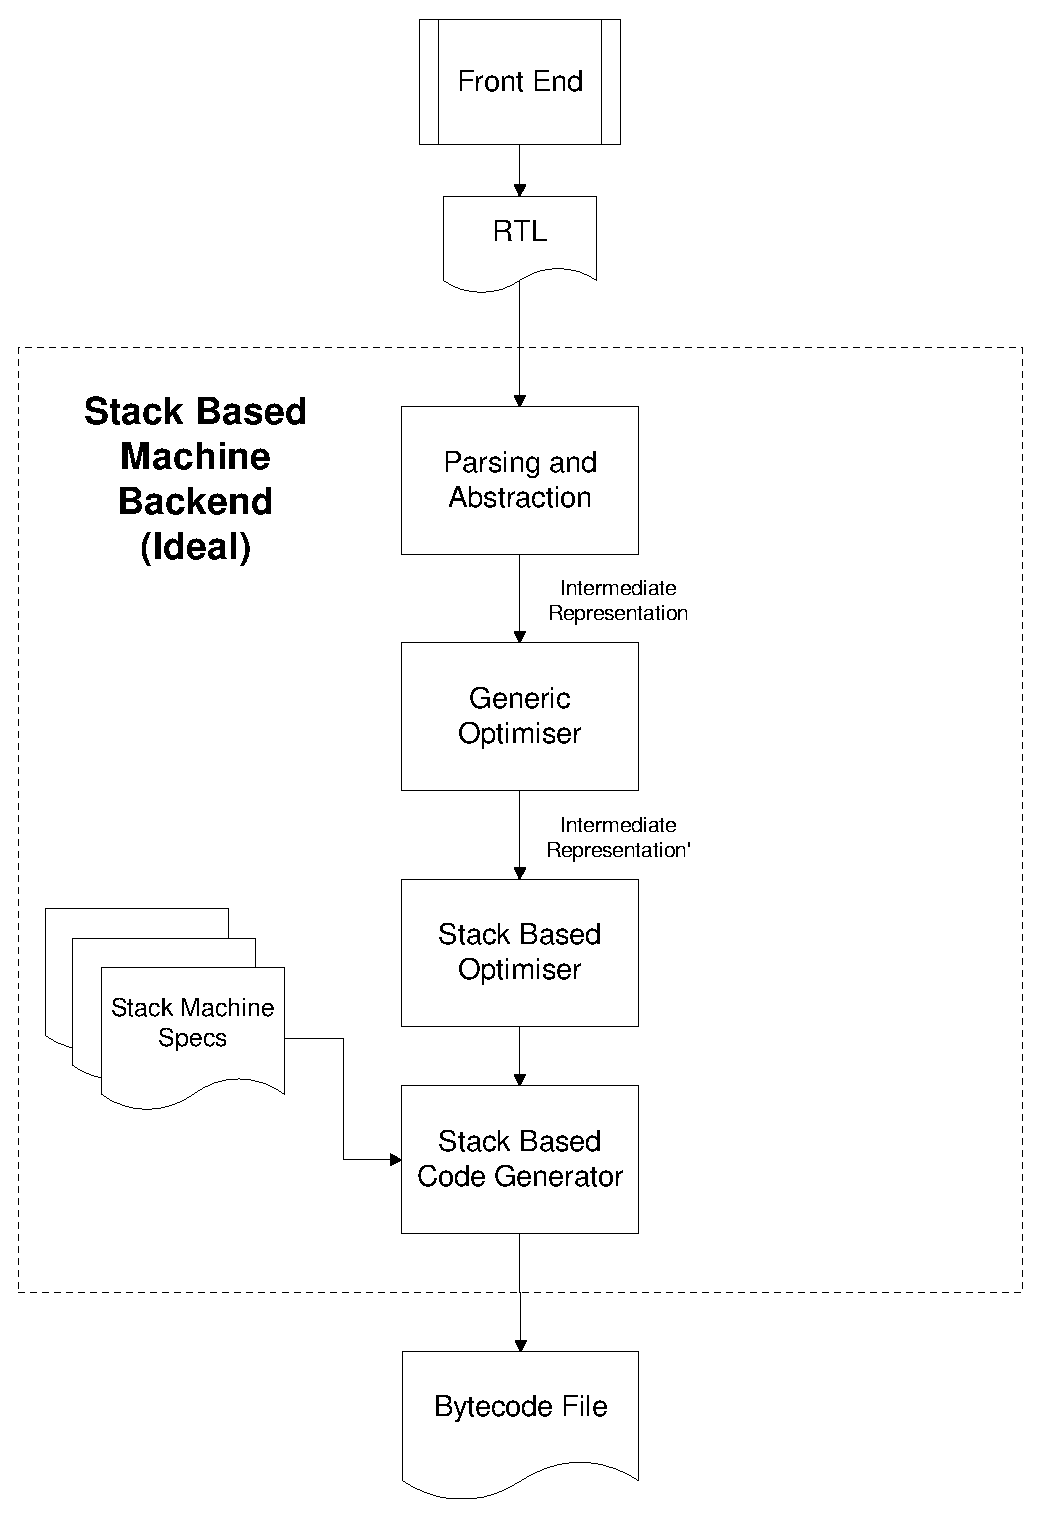
\includegraphics{figures/sbmbflow.eps}}
\centerfigend{fig-sbmbflow}{Flow Chart of the Stack Based Machine Backend}

\begin{enumerate}
\item Parsing and abstraction:  reduction of register transfer list
representation to basic assignment, call and branch statements.
\item Generic optimiser:  machine independant optimisation of those
statements.
\item Stack based optimiser:  stack based machine specific optimisations.
\item Stack based code generator:  generation of translated bytecodes
from the output of previous steps.  In the idealised model, the stack
based code generator can take a number of specification files that define
the target stack based machine.
\end{enumerate}

Each of these stages has an interface that interconnects them.  The
interface generated from parsing and abstraction of the RTL is used in the
optimiser.  This interface is known as the ``intermediate representation''
and consists of a control flow graph with each basic block containing an
array of statements.  The optimisers generate the same interface as they
receive, and as such, can be removed from the process when optimisations
are not required (such as in testing).  The code generator extends the
interface output from the optimiser with bytecode information placed in
each of the statements contained within a basic block. This data is then
linearised into an output file for the required machine.

The process depicted in figure ~\ref{fig-sbmbflow} is an idealisation of
the current experimental model of the stack based machine backend.  The
current process is better depicted in figure ~\ref{fig-sbmbflowcur} with
the difference being the final stage of processing.  Currently, the stack
based machine backend is targeted at the Java Virtual Machine and will be
hand extended to other stack based machines by rewritting this final
stage.  Once this is done, it will be easier to generalise about stack
based machines and approach the prefered model of absolute
retargetability.

\centerfigbegin
\resizebox{8cm}{!}
{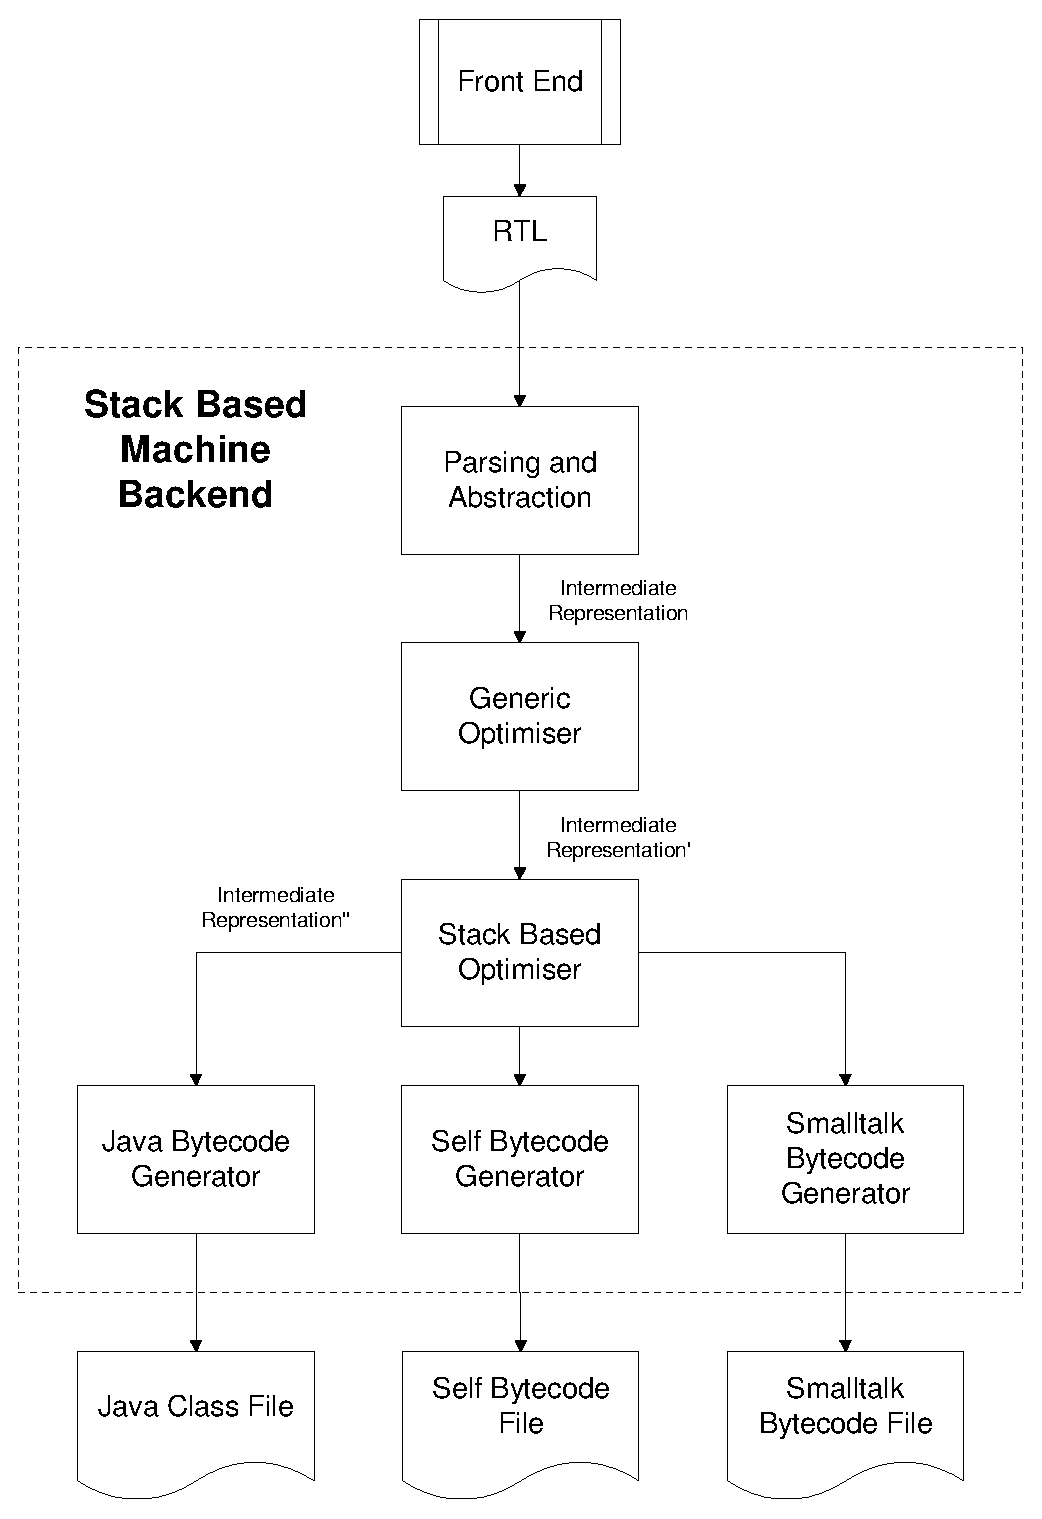
\includegraphics{figures/sbmbflowcur.eps}}
\centerfigend{fig-sbmbflowcur}{Experimental flow chart of the Stack Based Machine Backend}

\subsubsection{Intermediate Representation}

The intermediate representation consists of a control flow graph, that is,
a set of interconnected ``basic blocks''.  A basic block is defined as
having only one entry point and one exit point.  As control flows through
a program it follows a path that can be plotted.  If one was to plot all
the possible paths through a program, one would be constructing a control
flow graph.  In this way, a frontend programmer can use any form of
control structures in their language without fear of having to implement
them in the backend.  For example, an \texttt{if-then-else} structure
consists of four basic blocks.  The first basic block contains the
expression being tested.  If the expression is true, control flows to the
second basic block.  If the expression is false, control flows to the
third basic block.  Both the second and the third basic blocks fall
through to the fourth basic block.

\centerfigbegin
\resizebox{3cm}{!}
{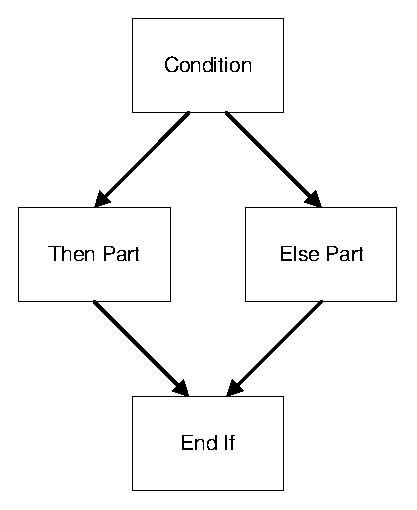
\includegraphics{figures/ifthenelse.eps}}
\centerfigend{fig-ifthenelse}{Control Flow Graph of an If-Then-Else
construct}

The first basic block is said to have two out-edges. The fourth basic
block has two in-edges.  A pretested loop is constructed just as easily.

Each basic block in the control flow graph contains an array of
statements.  These statements are mainly assignment statements but some
are also call statements.  Basic blocks which have two out edges (called
``two-ways'') have an extra statement attached, the ``conditional
statement''.  Statements are made up of expressions.  An expression can be
many things including arithmetic operations, logical operations, call and
assignment operations.  Each expression may have a number of parameters.
Expressions with two parameters are the binary expressions (add, multiply,
divide, etc).  Expressions with one parameter are the unary expressions
(negate, not, etc).  Unary expressions store their one parameter in the
``left'' node whereas binary expressions use both the ``left'' and
``right'' nodes.

These parameters are used to construct a tree structure for each
statement.  An optimiser will walk this tree structure and perform
optimisations that modify the structure.  A code generator will walk the
tree structure and generate code to be placed in various nodes of the
tree.  Both these uses of the tree structure require additional
information to be added to various nodes.  Specifying this data in the
intermediate representation classes would be non-generic and may result in
bloated trees filled with data that never gets used.  This method would
also mean that the intermediate representation would have to be changed
with every new use of the structure.  One would have to be very careful to
not ``break'' the data structure by removing anything that a user of a
previous version of the data structure may have assumed would never
change.  A solution to this problem is to allow the extension of
``objects'', that is, the instantiation of classes, not just classes
themselves.  To do this, each Java class in the implementation of the
intermediate representation is defined as an extension of the
``Extendable'' class.  A method can now be written to extend any of these
classes in such things as an optimiser or a code generator.

\subsubsection*{Data structure of the intermediate representation}

The Intermediate Representation contains a number of classes that
form a hierarchical structure of usage:
\begin{description}
\item [Program] is used to represent a complete program.  It contains an
array of procedures.
\item [Procedure] is used to represent a single procedure.  It contains
the name of the procedure and a control flow graph.
\item [BasicBlock] is used to construct a control flow graph.  It contains
a type, an array of in-edges, an array of out-edges, and an array of
statements.  Basic blocks of the \texttt{twoway} type contain a
\texttt{condition statement} which is used to determine which of the two
out-edges are followed during program execution.
\item [Expression] is used to construct statements.  Expressions contain a
type, a single integer parameter, and left and right expressions depending
on the expression type.  \texttt{Call} expressions contain an array of
expressions that are the parameters to the call.
\end{description}

\subsection{Examples}

The following examples show the current state of the UQBT frontend and the
stack based machine backend.  The following C program tests
assignments and simple conditional branches.  It is written on the SPARC 
archetecture:
\begin{verbatim}
void main() {
int i,j,k;

  j = i+k;
  k=6;
  i=j+5;

  printf("%i\n",i);
  if (j<k) 
    printf("%i\n",j);
  printf("%i\n",k);

}
\end{verbatim}
UQBT generates an output file which is parsed by the stack based machine
backend into the following statements in the intermediate representation.
\begin{verbatim}
proc main

bb type call
r[8] := r[48] 
r[9] := r[50] 
r[8] := r[8] + r[9] 
r[49] := r[8] 
r[8] := 0 | 6 
r[50] := r[8] 
r[8] := r[49] 
r[9] := r[8] + 5 
r[48] := r[9] 
r[9] := 69 << 10 
r[8] := r[9] | 552 
r[9] := r[48] 
Call printf(r[8],r[9])  

bb type twoway
r[8] := r[49] 
r[9] := r[50] 
r[0] := r[8] - r[9] 
bb cond: r[0] >= 0 

bb type call
r[9] := 69 << 10 
r[8] := r[9] | 552 
r[9] := r[50] 
Call printf(r[8],r[9])  

bb type call
r[9] := 69 << 10 
r[8] := r[9] | 552 
r[9] := r[49] 
Call printf(r[8],r[9])  

bb type ret
\end{verbatim}
These statements are passed to the code generator for Java, which adds
bytecode information to each of the nodes in the Intermediate 
Representation. Note that optimisation has been disabled for this example.  
The Intermediate Representation is then flattened to produce an output
file.  Comments have been added for clarity:
\begin{verbatim}
L0:
        iload 48        ; r[8]  := r[48]
        istore 8
        iload 50        ; r[9]  := r[50]
        istore 9
        iload 8         ; r[8]  := r[8] + r[9]
        iload 9
        iadd
        istore 8
        iload 8	        ; r[49] := r[8]
        istore 49
        ldc 0           ; r[8]  := 0 | 6
        ldc 6
        ior
        istore 8
        iload 8         ; r[50] := r[8]
        istore 50
        iload 49        ; r[8]  := r[49]
        istore 8
        iload 8         ; r[9]  := r[8] + 5
        ldc 5
        iadd
        istore 9
        iload 9         ; r[48] := r[9]
        istore 48
        ldc 69          ; r[9]  := 69 << 10
        ldc 10
        ishl
        istore 9
        iload 9         ; r[8]  := r[9] | 552
        ldc 552
        ior
        istore 8
        iload 48        ; r[9]  := r[48]
        istore 9
        iload 8         ; Call  printf(r[8],r[9])
        iload 9
        invokestatic printf
        goto L1

L1:
        iload 49        ; r[8]  := r[49]
        istore 8
        iload 50        ; r[9]  := r[50]
        istore 9
        iload 8         ; r[0]  := r[8] - r[9]
        iload 9
        isub
        istore 0
        iload 0         ; bb cond: r[0] >= 0
        ldc 0
        if_icmplt L2
        goto L3

L2:
        ldc 69          ; r[9]  := 69 << 10
        ldc 10
        ishl
        istore 9
        iload 9         ; r[8]  := r[9] | 552
        ldc 552
        ior
        istore 8
        iload 50        ; r[9]  := r[50]
        istore 9
        iload 8         ; Call  printf(r[8],r[9])
        iload 9
        invokestatic printf
        goto L4

L3:
        ldc 69          ; r[9]  := 69 << 10
        ldc 10
        ishl
        istore 9
        iload 9         ; r[8]  := r[9] | 552
        ldc 552
        ior
        istore 8
        iload 48        ; r[9]  := r[49]
        istore 9
        iload 8         ; Call  printf(r[8],r[9])
        iload 9
        invokestatic printf
        goto L2

L4:
        ret

\end{verbatim}
This bytecode is unoptimised which is to be expected as the Intermediate
Representation is unoptimised.  The generic optimiser reduces the number
of statements in the intermediate representation.  The stack based 
machine optimiser uses specific stack based machine optimisations to
reduce the number of bytecodes, local variables and stack depth.  Finally,
the code generator for the Java Virtual Machine selects the best bytecodes
to be used in the final output.

\subsection{The Runtime Environment}

Binary translation is not just a compiler backend (though it can be).  
Generally, there is a lot of code that can be shared between translated
programs.  This code has the task of emulating the environment that the
code was originally written for.  Such things as calling conventions and
dynamic linking must be known to the backend to generate code that can
link to its new environment.  We can see the need for a run time
environment through a case study.  The following C program:
\begin{verbatim} 
void main() {
  printf("hello world\n");
}
\end{verbatim}
compiles to the following assembly code (some code is removed for the
purpose of readability):

\begin{verbatim} 
.LLC0:
        .asciz  "hello world\n"

        sethi %hi(.LLC0),%o1
        or %o1,%lo(.LLC0),%o0
        call printf,0
        nop
        ret
\end{verbatim}

which can be translated and optimised to:
\begin{verbatim} 
        r[0] := .LLC0;
        call printf
        return 
\end{verbatim} 

Finally we can add to this
code the knowledge of calling convention.  On a SPARC, parameters are
passed in the first six general purpose integer registers.  The function
\texttt{printf} expects to see a pointer to an asciiz string as its first
parameter.  This is a problem in Java, for example, because \texttt{.LLC0}
refers to an offset in the source binary's read-only data section.  The
translated program will need access to this data if it is to pass the
string onto a function like \texttt{System.out.println}. The problem is
actually harder than that.  \texttt{System.out.println} expects a
\texttt{String} object type which is quite different to an asciiz string.  
The translated program will need to construct such an object using a
method not unlike the following:
\begin{verbatim} 
static String getstring(int rodatastart,byte[] rodata,int i) {
    String a = "";
      while (rodata[i-rodatastart]!=0) {
        a += (char)rodata[i-rodatastart];
        i++;
      }
      return a;
  }
\end{verbatim} 
The first parameter is the source machine address of the start of the
read-only data section.  The second parameter is a reference to the actual
bytes contained within the read-only data section.  The final parameter is
the source machine address of the asciiz string which we assume to be
located somewhere within the read-only data section.  We refer to this
calling structure as ``passing core'' and it must be used in all runtime
support libraries.

Finally the \texttt{printf} function must be written in Java to link with
the translated binary.  The function could be as simple as a wrapper to
the equivalent Java function or, in the case of printf, something more
complicated.  This must be done for every library function to be called.  
The size of a run-time environment is extensive in the case of graphical
user interface (GUI) environments.  This can be seen in the WINE
project~\cite{Wine96} which aims to emulate the Microsoft Windows
environment on 80x86 X-windows systems.  We can reuse most of the work in
that project.  This promotes the feasibility of binary translation of
Windows executables to the JVM with an interface to the awt classes.  The
biggest obstacle of the WINE project is the Application Binary Interface
(ABI) of Microsoft Windows.  Each binary refers to more than its own data
segments and system API calls.  In many operating systems, applications
have access to data structures stored in shared libraries and, as in the
case of Microsoft Windows, in the operating system itself.  These
references must be recognised by the backend and replaced with a reference
to the runtime support class.  These problems are not limited purely to
Microsoft Windows (although they appear most abundantly there), they also
pop up in SPARC binaries.  One such example is the use of \texttt{errno}
from the standard I/O C libraries.  \texttt{Errno} is a global integer
that resides in a shared library.  When it is written to, the page that is
shared is copied into the new process space.  One would wish a backend to
recognise global variables that reside in support libraries and redirect
them to the runtime support class.


\subsection{Summary}

The development of backends borrows heavily from the field of optimising
compilers.  The targeting of a backend to a stack based machine introduces
new problems in optimisation.  The JVM and its strict typing introduces
problems that have rarely been seen by compiler writers before.  A runtime
support library is necessary to minimize the size of the translated
applications and is specific to each source machine and platform.  The
development of a binary translator to Java bytecodes promises a new
mentality in application distribution.  The ``translate once, run
anywhere'' concept is already within our reach, what still awaits is a
resultant application that runs with a similar performance on the JVM as
on the source machine.  This work outlines the steps involved in such a
backend and takes the first tentative steps towards that end.



\section{gcc-jvm - A JVM Backend for the gcc Compiler} 
\label{sec-gccjvm}

{\small
\begin{flushright}
Design: Trent, Implementation: Trent, Documentation: Trent [Aug 99]
\end{flushright}
}

This section describes Trent's experiences with porting
EGCS (gcc version 1.1.2) to a stack-based machine, 
the JVM in particular.  It is written in first person.  

When I first began investigating the possibility of porting the
Experimental GNU Compilation Set (EGCS) to the Java Virtual Machine (JVM)
I thought it would be possible to semantically describe the JVM to EGCS
and have it adequately generate stack based machine byte codes.  I hoped
that I would be able to specify to the back end that the only way to load
a constant or a register (local variable) was via the stack and EGCS would
break its internal representation effectively.  This appears to be a
little too optimistic.  My attempts at constructing a machine description
where EGCS is forced to do all moves via the stack failed, not because I
was supplying too little information to the back end, but because I was
supplying too much.  This lead to an alternate strategy:  I decided to
take all the instructions that one would find on a register based machine
and implement them using a number of byte codes.  The resultant byte code
was a poor but correct representation of the original program.  Soon I had
simple programs (hello world) working and could actually perform some
benchmarks.  The results were astounding: small register transfer bound
programs ran at comparable speeds to native code.  This is best explained
with an example.

\begin{verbatim}
int fibo(int i) {
  if (i<2) return 1;
  else return fibo(i-1)+fibo(i-2);
}

void main(int argc,char **argv) {
  printf("fibo %i is %i\n",40,fibo(40)); 
}
\end{verbatim}

Fibonacci is a register transfer bound program that takes 22 seconds on a
SPARC Ultra 9 to run natively.  If we compile it to JVM byte code we get
the following (for the fibo function).

\begin{verbatim}
.method public _fibo(I)I
        .limit stack 9
        .limit locals 17
        
        iconst_0
        istore 14
        
        iload 1
        bipush 1      
        if_icmple L2
        
        iload 1  
        bipush -1
        iadd
        istore 10
        
        aload_0
        iload 10
        invokevirtual Fibo/_fibo(I)I
        istore 10   
        
        iload 10 
        istore 13
        iload 1  
        bipush -2
        iadd   
        istore 10
        
        aload_0     
        iload 10
        invokevirtual Fibo/_fibo(I)I
        istore 10
        
        iload 13 
        iload 10 
        iadd   
        istore 10
        
        goto L8     
L2:
        bipush 1
        istore 10

L8:
        iload 10 
        ireturn
.end method
\end{verbatim}

On the same machine running version 1.1 of the JVM, this bytecode takes
90 seconds to run.  The overhead is caused primarily by the two method
calls.  The following Java source code compiles to a program with the same
functionality.

\begin{verbatim}
class Fib {

  int fibo(int i) {
    if (i<2) return 1;
    else return fibo(i-1)+fibo(i-2);
  }

  void main(int argc,int argv) {                 
    System.out.println("fibo " + 40 + " is " + fibo(40));         
  }

  public static void main(String[] args) {
    Fib f = new Fib();
    f.main(0,0);
  }
}
\end{verbatim}

The resultant class file takes 56 seconds to run.  Significantly less than
the EGCS generated byte code.  The following is the byte code that is
generated by javac (for the fibo method above).

\begin{verbatim}
Method int fibo(int)
   0 iload_1
   1 iconst_2
   2 if_icmpge 7
   5 iconst_1
   6 ireturn
   7 aload_0
   8 iload_1
   9 iconst_1
  10 isub
  11 invokevirtual #13 <Method int fibo(int)>
  14 aload_0
  15 iload_1
  16 iconst_2
  17 isub
  18 invokevirtual #13 <Method int fibo(int)>
  21 iadd
  22 ireturn   
\end{verbatim}

Smaller size and less local variable usage improves the speed of the byte
code.  A possible solution to this problem is to use a post processing
optimisation stage such as BLOAT.  When applied to the poor byte code
generated by EGCS, it produces the following.

\begin{verbatim}
Method int _fibo(int)
   0 iload_1
   1 iconst_1
   2 if_icmple 31
   5 iload_1
   6 iconst_m1
   7 iadd
   8 istore_2
   9 aload_0
  10 iload_2
  11 invokevirtual #20 <Method int _fibo(int)>
  14 istore_2
  15 iinc 1 -2
  18 aload_0
  19 iload_1
  20 invokevirtual #20 <Method int _fibo(int)>
  23 istore_0
  24 iload_2
  25 iload_0
  26 iadd
  27 istore_0
  28 goto 33
  31 iconst_1
  32 istore_0
  33 iload_0
  34 ireturn
\end{verbatim}

This is still a lot more bytecodes than the javac generated output but
runs in 55 seconds.  This leads to an apparent paradox:  How can more 
bytecodes run faster than less byte codes?  The answer lies in the behaviour
of the Just In Time compiler.  For version 1.1 of the JVM one can export
an environment variable JIT\_ARGS to 'dump' to print excessive amounts of
debugging information.  Using the bash shell one would do the following
command:
\begin{verbatim}
		export JIT_ARGS=dump
\end{verbatim}

Now any execution of the JVM will result in JIT debugging information
being dumped to standard error.  For version 1.2 of the JVM one would do
the following command:
\begin{verbatim}
		export _JIT_ARGS=dump
\end{verbatim}

The following is output by the JIT for the javac generated bytecode:
\begin{verbatim}
     0 iload_1        1b     
     1 iconst_2       05           
     2 if_icmpge      a2 00 05
        subcc   %i1, 2, %g0
        bge     5
        nop     
     5 iconst_1       04     
     6 ireturn        ac
        or      %g0, 1, %i0
        ba      8
        nop        
     7 aload_0        2a           
     8 iload_1        1b     
     9 iconst_1       04
    10 isub           64   
        sub     %i1, 1, %l0           
    11 invokevirtual  b6 000d
        or      %l0, %g0, %o1
        or      %g0, %i0, %o0
        ld      [%o0 + 4], %g1
        ld      [%g1 + 52], %g1
        ld      [%g1 + 68], %g1
        jmpl    [%g1 + %g0], %o7
        nop
        unimp   0x000a5a78 
        or      %g0, %o0, %l0    
    14 aload_0        2a        
    15 iload_1        1b        
    16 iconst_2       05    
    17 isub           64
        sub     %i1, 2, %l1        
    18 invokevirtual  b6 00 0d
        or      %l1, %g0, %o1
        or      %g0, %i0, %o0
        ld      [%o0 + 4], %g1
        ld      [%g1 + 52], %g1
        ld      [%g1 + 68], %g1
        jmpl    [%g1 + %g0], %o7
        nop
        unimp   0x000a5a78 
        or      %g0, %o0, %l1    
    21 iadd           60
        add     %l0, %l1, %l0        
    22 ireturn        ac
        or      %g0, %l0, %i0
\end{verbatim}
  
The major overhead of the above code being the two method calls.  
Ignoring the method calls, ten native machine instructions are generated.  
The following is output for the BLOAT optimised EGCS output:
\begin{verbatim}
     0 iload_1        1b     
     1 iconst_1       04     
     2 if_icmple      a4 00 1d
        subcc   %i1, 1, %g0
        ble     5
        nop     
     5 iload_1        1b    
     6 iconst_m1      02
     7 iadd           60
        add     %i1, -1, %i2          
     8 istore_2       3d           
     9 aload_0        2a     
    10 iload_2        1c     
    11 invokevirtual  b6 0014
        or      %i2, %g0, %o1
        or      %g0, %i0, %o0 
        ld      [%o0 + 4], %g1
        ld      [%g1 + 200], %g1
        ld      [%g1 + 68], %g1
        jmpl    [%g1 + %g0], %o7
        nop
        unimp   0x000a5b60
        or      %g0, %o0, %l0
    14 istore_2       3d
        or      %g0, %l0, %i2         
    15 iinc           84 01fe   
        add     %i1, -2, %i1           
    18 aload_0        2a        
    19 iload_1        1b    
    20 invokevirtual  b6 0014
        or      %i1, %g0, %o1 
        or      %g0, %i0, %o0
        ld      [%o0 + 4], %g1  
        ld      [%g1 + 200], %g1
        ld      [%g1 + 68], %g1
        jmpl    [%g1 + %g0], %o7
        nop
        unimp   0x000a5b60
        or      %g0, %o0, %l0    
    23 istore_0       3b
        or      %g0, %l0, %i0        
    24 iload_2        1c        
    25 iload_0        1a           
    26 iadd           60  
        add     %i2, %i0, %i0    
    27 istore_0       3b        
    28 goto           a7 0005
        ba      1e
        nop    
    31 iconst_1       04
    32 istore_0       3b
        or      %g0, 1, %i0    
    33 iload_0        1a    
    34 ireturn        ac
\end{verbatim}

Again ignoring the two method calls, eleven native machine instructions
are generated.  One can now see that byte code size is not an entirely
fair measure of resultant JIT generated code size.

The introduction of local variable usage that cannot be mapped into
registers (for example, local arrays) a register based machine requires a
stack frame.  Commonly, a stack pointer and a frame pointer are maintained
to point to a section of volatile memory.  This posses a problem for the
JVM port: there is no generic memory.  Possible solutions are to maintain
a "stack" array of bytes and do all stack accesses to that array.  The
problem becomes more complex when one considers global memory.  The
solution I originally chose was to perform all memory input/output with a
method contained within a run time support class.  The method to read an
integer from any arbitrary point in memory was called memref and the
method to store an integer to any arbitrary point in memory was called
memstore.  These two methods would examine the address requested and
determine the required array reference: read only data, read/write data or
stack.  To perform a memory reference the backend need only generate the
following:
\begin{verbatim}
sipush 24324   ; address
invokevirtual Classname/memref(I)I
istore 9
\end{verbatim}

The resultant bytecode was very easy to read and could be easily debugged
(for example, one could monitor all reads and writes to memory).  
Unfortunately memory bound programs experienced dramatic performance
losses.  In the order of sixty times slower execution.  The solution was
to move all memory references inline and abandon the array segregation.  
All memory was placed in a single array, called "memory", in the run time
support class and now the back end is required to generate significantly
more code.  To load an integer from an unsigned byte array one need only
perform the following (big endian).

\begin{verbatim}
Register := memory[location] << 24 | 
    memory[location+1] << 16 | 
    memory[location+2] << 8 | 
    memory[location+3]
\end{verbatim}

However, the JVM does not have unsigned types, and thus each signed byte
must be converted to an integer representation of its unsigned value:
\begin{verbatim}
Register := (memory[location]<0?256+memory[location]:memory[location]) << 24 | 
    (memory[location+1]<0?256+memory[location+1]:memory[location]) << 16 | 
    (memory[location+2]<0?256+memory[location+2]:memory[location+2]) << 8 | 
    (memory[location+3]<0?256+memory[location+3]:memory[location+3])
\end{verbatim}

To improve the performance of each integer memory reference, the memory
array is made an array of int instead of an array of byte.  Initialised is
then put into the array already in unsigned format.  The speed increase
comes at the expense of a 4:1 increase in space requirements.  The
following code is generated by the back end to perform an integer memory
reference:
\begin{verbatim}
        aload_0
        getfield Classname/memory [I
        iload 12 ; address
        dup2  
        iaload  
        bipush 8
        ishl
        dup_x2
        pop 
        iconst_1
        iadd
        dup2
        iaload   
        bipush 16
        ishl    
        dup_x2  
        pop 
        iconst_1
        iadd
        dup2
        iaload
        bipush 8
        ishl     
        dup_x2   
        pop     
        iconst_1
        iadd
        iaload  
        ior 
        ior 
        ior
        istore 11  ; destination
\end{verbatim}

The same memory bound benchmarks now run at 20 to 30 times as slow.  
Memory management is still a significant issue that is difficult to
resolve.


\subsection*{The build process}

The output of the compiler proper is one jasmin~\cite{Meye97} 
assembler file per C language input file.  
If the input files contain no global data, the build
process is simple, concatenate the multiple jasmin files into a single
file and assemble to a class file.  However, C files containing global
data produce an addition output file global.s.  References to labels
contained in global.s will appear in the jasmin output preceded by
"symref" and proceeded by "end".  As each C input file is compiled, the
global.s outputs are concatenated together into gglobal.s.  This file is
assembled to object format and a search and replace program (sed) is used
to replace each symbol reference with an offset into the data section.  
Finally the object file is objcopied into a raw data file and passed to
the run time support class to be loaded into the memory array.  This
process is only needed in programs with multiple input files and global
data.


\section{The Java JVM Back end}
\label{sec-jvmbackend}

{\small
\begin{flushright}
Design: Cristina and Brian, Implementation: Sameer [Aug 00], Brian [Nov 00],  
	Documentation: Brian [Nov 01]
\end{flushright}
}

The Java JVM back end is a rewrite of the C-based original JVM 
back end that was written in early 1999.  We were interested in 
seeing whether the Java language could be used to write back ends 
for our translator needs.  The following notes explain part of the
operation of this back end. 
Experience with the user of this back end is described in the 
{\emph{Experience}} chapter (Chapter~\ref{ch-experience}) in 
Section~\ref{sec-to-jvm}.  

The Java JVM backend operates much like the C and other backends. 
Unlike the C (Chapter~\ref{ch-cbackend}) and the VPO (Chapter~\ref{ch-vpobackend}) 
backends, however, it is single-pass. The Jasmin code for each procedure is
emitted in one pass. A small runtime library implemented in the file
\texttt{TranslatedFile.java} provides support for the generated code. That 
file contains a method \texttt{realMain} that is called first when the 
translated program starts execution. The \texttt{realMain()} method 
initializes the memory used by the translated program and copies the program's 
command line arguments into that memory.  The \texttt{realMain()} method 
then calls the translated program's \texttt{\_main()} method, which contains 
the code for the program's main procedure. All generated methods are static 
except for \texttt{\_main()}. This is done for technical reasons 
(\texttt{\_main} is declared abstract in \texttt{TranslatedFile.java}).

It recursively processes a source procedure's HRTLs for a procedure and
emits directives for each HRTL into a Jasmin source file. Given a HRTL, it
checks first whether it is a high-level HRTL such as a CALL\_HRTL, or if it
is a RTLList, a list of low-level RTLs. If the former, directives for the
control transfer or other high-level HRTL are emitted. If the latter,
directives for each RTL in the list are emitted. A postorder traversal of
each RTL's subexpressions produces the stack-oriented JVM bytecodes for that
RTL. 

Memory is represented using a single large Java byte array "memory". The
source program's bss and data segments are read into the appropriate
elements of that array so that a data item at a particular
address x can be read from memory[x].

The most complex thing (perhaps) about the JVM backend's operation is its
allocation of JVM locals for the HRTL variables:

\begin{itemize} 
\item Local 0 always holds the Java \texttt{this} reference if the procedure 
	is \texttt{\_main()}, and the first procedure argument otherwise.
\item Locals 1-7: all or remaining formal parameters (assumes there are 
	up to 6 parameters at most).
\item Local  8 and 9: unused.
\item Local [10..(10+n)): the n local HRTL variables used in the method.
\item Locals [(10+n)..99]: the HRTL temporary registers.
\item Local 100: a temporary variable used for, e.g., byte swapping.
\end{itemize}


\subsection{Usage of the Java JVM Backend}
To use the JVM backend,
build \uqbt\ with \texttt{with-target=sparc}
and then request the JVM backend using the command line option \texttt{-j}.
This will make \uqbt use the JVM backend
rather than the default low-level \texttt{C} backend.
The \texttt{Makefile} generated in the output directory created by \uqbt\ 
includes rules to run Jasmin and build the necessary Java class files for
the translated program.


	 % JVM backend (two different versions) 

	
\chapter{The VPO Back End}
\label{ch-vpobackend}

{\small
\begin{flushright}
Design: Mike, Cristina, Norman. Implementation: Mike [98], Brian [01]. 
Documentation: Mike [98], Cristina, Brian [01]
\end{flushright}
}

In early 1998 we were using the VPO (very portable optimizer) system  
by Jack Davidson and students, University of Virginia, as our 
optimizer of choice.  We experimented with SPARC translations 
before we moved onto the C back end (see Chapter~\ref{ch-cbackend}). 
VPO's RTL interface back then was new and did not support x86 or 
other machines yet. 
The 1998 VPO back end is described in Section~\ref{sec-vpo}. 
This section is useful for historical reasons. 

In 2001 we went back to use VPO for optimization, by then, VPO's 
new RTL interface supported not only SPARC, but also x86 and ARM 
amongst other machines.  We were interested in translations to 
these three machines.  The original 1998 VPO back end was revived 
in a new form and made much more extensible and robust. 
The 2001 VPO back end is described in two parts: first, the 
experiment in translating IRTL to SPARC VPO RTLs is described in 
Section~\ref{sec-irtlvpo}, and next, the experiences with translating 
\hrtl\ to ARM VPO RTLs are described in Section~\ref{sec-vpo2001}. 


\section{The 1998 VPO Back End}
\label{sec-vpo}

This section describes \texttt{vpoback}, an experimental RTL$_{UQ}$
to RTL$_{VPO}$ translator which generates a file suitable for
piping to VPO, so that an executable file can be generated.
This backend is not meant to
be a serious prototype for a real backend, but is intended to demonstrate
the compatibility of the two RTLs. The experiment was
a success; it was possible to translate enough RTLs to generate a simple 
``hello world'' binary executable file for the SPARC platform (from 
a SPARC source binary).


\subsection{Description}

The experimental backend has been written to work with a preliminary
version of the VPO interface, as supplied by the University of Virginia 
in February 1998. This version has two distinct interfaces; one to generate 
Register Transfer Lists, and one to handle higher level concepts such as 
functions and global symbols. All functions of the first interface have 
names beginning with \texttt{Rtl\_}, while functions of the latter interface 
have names beginning with \texttt{VPOi\_}.


\subsection{Handling expressions}
\label{sec-expr}

In general, expressions in VPO are very similar to expressions in our
RTlists. For binary expressions, there are two considerations when
translating from RTL$_{UQ}$ to RTL$_{VPO}$. Firstly,
the operators have to be translated. Secondly, the \texttt{sethi}
instruction has to be considered specially. Most of our operators have
direct VPO equivalents. Notable exceptions are rotates with carry
(RTL$_{VPO}$ does not have them), and bit extractions (RTL$_{VPO}$ does
not appear to have them).

When translating the \texttt{sethi} instruction, it was found necessary
to translate
expressions of the form \verb!K << 10! (where K is a constant, and
\verb!<<! represents the left shift operator) to expressions like
\texttt{HI[X]}, where \texttt{HI} is a special Sparc specific unary
operator in VPO, and X has the value \verb!K<<10!.


\subsection{Handling registers}

Normal machine registers, such as r[8] (and even r[0] for register \%g0)
translate
directly to VPO using the \texttt{Rtl\_constLoc()} function. Some registers
are named (i.e. they are represented as a \texttt{Register} object, whose
\texttt{Index} member points to an object of type \texttt{Constant}, whose
value is a string, e.g. ``\%fp''). Others are implemented as special
registers (i.e. they are represented as a \texttt{SpecialReg} object).
SpecialReg objects have a name (it could also be \texttt{\%fp}; both
representations exist at present). These named registers
are translated into the appropriate general purpose register (\texttt{\%fp}
maps to register 30, and \texttt{\%sp} maps to register 14).

Temporary registers (e.g. \texttt{r[\_\_tmp123]}) are translated to ordinary
registers beginning with index 51 (for texttt{r[\_\_tmp001]}). VPO is to be
changed so that temporary registers will occupy their own storage spaces.


\subsection {Handling memory}

An object of class Memory contains a pointer to a Value object, which
could be of three types: \texttt{eCONSTANT}, \texttt{eREGISTER}, or
\texttt{eSPECIALREG}. These
represent the address of the memory being referenced. Where the address
is constant, the \texttt{Rtl\_constLoc()} function is used. Where the address
is given as a register, the register is processed as a location. This
location is fetched using \texttt{Rtl\_fetch()}, and the resultant expression
is used as the operand to \texttt{Rtl\_location()}.


\subsection {Handling RT assignments}

RT assignments involve a location and an expression. The location will
be either a register or memory object; each of these is translated to
a VPO location as above. The expression is also translated as previously
described (section~\ref{sec-expr}).
Where registers or memory are involved in the expression, they are translated 
as described above, and the result is converted into a value using
the \texttt{Rtl\_fetch()} function. The location and expression resulting
from the above (of types \texttt{Rtl\_ty\_loc} and \texttt{Rtl\_ty\_expr}
respectively) are
combined and emitted using the \texttt{VPOi\_rtl()} interface function.


\subsection {Handling Control Transfer instructions}

All the above translations are handled by considering a single Register
Transfer (RT) at a time. Basically, each RT of each RTL in the function
of interest is examined in a double counter for loop. However, there are a few
situations that have to be handled by examining a whole RTL; control
transfer instructions and frame instructions are examples. Complex
code examines each RTL to see if it matches the pattern of the appropriate
instruction of interest; if so, code is emitted to VPO directly instead
of translating the whole list of RTs separately. It is hoped that changes
to the representation for RTL$_{UQ}$ will simplify this comparison.

If the instuction is recognised as a control transfer instruction, more
complex code decides whether the instruction is a conditional or
unconditional branch, call, or return instuction. (This complex, difficult
to debug code may one day be automatically be generated by some sort of
tool given a piece of specification or RTL tree).

Return instuctions are simple; an assignment from register \texttt{RT}
(a special
VPO pseudo register) to register texttt{PC} is emitted.

For a call instruction, a symbol has to be generated for the destination
of the call. (This will become a call to the ``assembly interface'' one
day; at present, it is a VPOi function). At the time of writing, the
names of dynamic symbols was not available, so the function name is
fixed at ``printf''. The call is generated by emitting an assignment to
special VPO register ST (``STack''?) from the global symbol for the
destination of the call. In order to convince VPO that main was not a
leaf function, we had to use the \texttt{VPOi\_registerUse()} function,
with an argument list including all registers
from 1 to 15, indicating that all these registers had to be saved across
the call (and therefore, leaf optimisation for the procedure containing
the call is not possible).

Unconditional branches are not implemented as of this writing; they should
present no special problems beyond those required for a call.

Conditional branches in VPO have the form \texttt{PC=IC:0,L1234} where
\texttt{PC} of course represents the program counter, \texttt{IC} represents
the integer condition code register, the colon represents a relational 
operator, and \texttt{L1234} represents
a label. This is emitted as a guarded assignment, using \texttt{Rtl\_guard()}
and \texttt{Rtl\_Rtl\_assign()}. The required operator has to be determined
from an
expression contained in the RTL for the branch instruction (it depends
on the condition codes used, as well as the operators, and whether
the condition code is used directly, or negated first). This is again
difficult to write code that may be automated in the future.

As an example of this process, consider the \texttt{bg} (branch if signed
greater) Sparc instruction. There are three RTs in the RTL; the
%main RT contains the subexpression \texttt{\~(\%Z \| (\%N \^ \%V))}
main RT contains the subexpression \verb!~(%Z | (%N ^ %V))!
(where \verb!~!
represents logical negation, and \verb!^! represents the exclusive OR
operator). When this subexpression is detected, the VPO opertor required
is \texttt{Rtl\_op\_gt}.

It was found that VPO does not have suitable operators for handling
the jump if positive/negative instructions, and jump on overflow /
no overflow.


\subsection {Processing Frame instructions}

The save and restore instructions (which establish and remove stack
frames) are recognised at the RTL level, just as conditional control
transfer instructions are. At present, only the restore instruction
is correctly recognised, and this is used to call the
\texttt{VPOi\_functionEnd()} function.


\subsection {Other VPO calls}

The function \texttt{premble()} calls several VPOi functions that are
needed to
initialise VPO itself, and to set up a label for \texttt{main}. These
functions
set up the register map and special location map; both of these are
going to be changed in the next version of the VPO interface.


\subsection {Sample Generated Code}

This output is from an early version. It should be replaced by a later
version.

The input file was compiled from the folowing source by {\it gcc}:
\begin{verbatim}
#include <stdio.h>

int main()
{
    int a=5; int b=7;
    unsigned u=5; unsigned v = 7;

    if (a == b) printf("Equal\n");
    if (a != b) printf("Not Equal\n");
    if (a >  b) printf("Greater\n");
    if (a <= b) printf("Less or Equal\n");
    if (a >= b) printf("Greater or Equal\n");
    if (a <  b) printf("Less\n");
    if (u >  v) printf("Greater Unsigned\n");
    if (u <= v) printf("Less or Equal Unsigned\n");
    if (u >= v) printf("Carry Clear\n");
    if (u <  v) printf("Carry Set\n");
}
\end{verbatim}

Generated output (filtered by the \texttt{decode} program and formatted for
3 columns):
\begin{verbatim}
-   .seg    "text"      +r[51]=r[8]             +r[16]=R[r[51]]
-    .global _start     +R[r[51]]=r[11]         +r[17]=r[14]-r[9]
-_start:                +r[51]=r[30]+20         +PC=ICs0,L67452
+r[30]=r[0]|0           +r[16]=R[r[51]]         +r[8]=66{10
+r[51]=r[14]+64         +r[51]=r[30]+24         +r[30]=r[0]|232
+r[16]=R[r[51]]         +r[16]=R[r[51]]         +r[51]=r[30]+28
+r[17]=r[14]+68         +r[17]=r[14]-r[9]       +r[16]=R[r[51]]
+r[17]=r[14]-32         +PC=IC!0,L67236         +r[51]=r[30]+32
+r[30]=r[0]|r[1]        +r[8]=66{10             +r[16]=R[r[51]]
+PC=IC:0,L66984         +r[30]=r[0]|144         +r[17]=r[14]-r[9]
+r[30]=r[0]|r[1]        +r[51]=r[30]+20         +PC=ICh0,L67488
+r[8]=66{10             +r[16]=R[r[51]]         +r[8]=66{10
+r[30]=r[0]|116         +r[51]=r[30]+24         +r[30]=r[0]|256
+r[30]=r[0]|r[16]       +r[16]=R[r[51]]         +r[51]=r[30]+28
+r[30]=r[0]|r[17]       +r[17]=r[14]-r[9]       +r[16]=R[r[51]]
+r[10]=r[16]{2          +PC=IC:0,L67272         +r[51]=r[30]+32
+r[17]=r[14]+4          +r[8]=66{10             +r[16]=R[r[51]]
+r[17]=r[14]+r[10]      +r[30]=r[0]|152         +r[17]=r[14]-r[9]
+r[8]=130{10            +r[51]=r[30]+20         +PC=ICl0,L67524
+r[30]=r[0]|572         +r[16]=R[r[51]]         +r[8]=66{10
+r[51]=r[10]            +r[51]=r[30]+24         +r[30]=r[0]|280
+R[r[51]]=r[11]         +r[16]=R[r[51]]         +r[51]=r[30]+28
*                       +r[17]=r[14]-r[9]       +r[16]=R[r[51]]
+r[8]=64{10             +PC=IC'0,L67308         +r[51]=r[30]+32
+r[8]=64{10             +r[8]=66{10             +r[16]=R[r[51]]
+r[30]=r[0]|824         +r[30]=r[0]|168         +r[17]=r[14]-r[9]
+r[17]=r[14]+r[15]      +r[51]=r[30]+20         +PC=ICg0,L67560
+r[8]=0{10              +r[16]=R[r[51]]         +r[8]=66{10
+r[30]=r[0]|4           +r[51]=r[30]+24         +r[30]=r[0]|296
+r[51]=r[23]+r[8]       +r[16]=R[r[51]]         +r[30]=r[0]|0
+r[16]=R[r[51]]         +r[17]=r[14]-r[9]       *
+r[51]=r[8]+4           +PC=IC>0,L67344         +r[8]=64{10
+r[16]=R[r[51]]         +r[8]=66{10             +r[8]=64{10
+r[17]=r[14]-0          +r[30]=r[0]|184         +r[30]=r[0]|308
+PC=IC:0,L67144         +r[51]=r[30]+20         +r[17]=r[14]+r[15]
+r[17]=r[14]+4          +r[16]=R[r[51]]         +r[8]=0{10
+r[51]=r[16]            +r[51]=r[30]+24         +r[30]=r[0]|8
+r[16]=R[r[51]]         +r[16]=R[r[51]]         +r[51]=r[23]+r[8]
+r[17]=r[14]+4          +r[17]=r[14]-r[9]       +r[16]=R[r[51]]
+r[51]=r[16]            +PC=IC<0,L67380         +r[51]=r[8]+4
+r[16]=R[r[51]]         +r[8]=66{10             +r[16]=R[r[51]]
+r[17]=r[14]-0          +r[30]=r[0]|200         +r[17]=r[14]--1
+PC=IC!0,L67116         +r[51]=r[30]+20         +PC=IC:0,L67660
+r[30]=r[0]|5           +r[16]=R[r[51]]         +r[17]=r[14]+-4
+r[51]=r[8]             +r[51]=r[30]+24         +r[51]=r[16]
+R[r[51]]=r[11]         +r[16]=R[r[51]]         +r[16]=R[r[51]]
+r[30]=r[0]|7           +r[17]=r[14]-r[9]       +r[17]=r[14]+-4
+r[51]=r[8]             +PC=IC`0,L67416         +r[51]=r[16]
+R[r[51]]=r[11]         +r[8]=66{10             +r[16]=R[r[51]]
+r[30]=r[0]|5           +r[30]=r[0]|224         +r[17]=r[14]--1
+r[51]=r[8]             +r[51]=r[30]+28         +PC=IC!0,L67632
+R[r[51]]=r[11]         +r[16]=R[r[51]]         *
+r[30]=r[0]|7           +r[51]=r[30]+32
\end{verbatim}

This is a brief summary of the interace functions used by \texttt{vpoback}.

\subsection {RTL Interface}
\begin{tabular}{l l}
Rtl\_unary      & Generates a unary expression \\
Rtl\_binary     & Generates a binary expression \\
Rtl\_fetch      & Converts a location to an expression \\
Rtl\_op\_special & Generates a special RTL operator \\
Rtl\_int        & Generates an integer as an expression \\
Rtl\_location   & Generates a location \\
Rtl\_constLoc   & Generates a location from a space and an index \\
Rtl\_assign     & Generates an RT assignment from a location and expression \\
Rtl\_guard      & Generates a sort of guard (for conditional branches) \\
Rtl\_label      & Generates a label (e.g. \texttt{L1234}) \\
Rtl\_globalSymbol & Generates a global symbol (e.g. \texttt{printf}) \\
\end{tabular}

\subsection {VPOi Interface}
\begin{tabular}{l l}
VPOi\_rtl		& Sends an RTL to output \\
VPOi\_registerMap 	& Sends a register map line to output \\
VPOi\_specialLocationMap & Tells VPOi about the special locations \\
VOIi\_assembly    	& Generate assembler directives \\
VPOi\_functionName 	& Tells VPOi about a function \\
VPOi\_functionEnd 	& Tells VPO and VPOi that a function has ended \\
VPOi\_variableDeclaration & Sends a variable definition to output \\
VPOi\_registerUse  	& Sends register use information to output \\
\end{tabular}


\section{Initial 2001 Experiments with VPO -- Translating IRTL to VPO RTLs}
\label{sec-irtlvpo}

{\small
\begin{flushright}
Design: Brian;
Documentation: Brian;
Implementation: Brian [June 01]
based on Mike's 1998 SPARC VPO backend.
\end{flushright} 
}

The IRTL Sparc-to-VPO backend uses the
University of Virginia's Very Portable Optimizer (VPO)
to generate optimized SPARC code
from an IRTL ({\em not} HRTL) representation of a source SPARC
program.
The quality of the optimized code is about the same as produced by gcc
with optimization level \texttt{-O4}.
IRTLs ({\em intermediate RTLs}) are a representation of programs
that is close to the machine level.
IRTLs differ from RTLs primarily in having
delayed branch instructions removed.
They differ from HRTLs in being source machine-specific
and not having the additional information about,
for example, procedure parameters and return values,
that results from expensive HRTL analysis.

This backend is experimental and incomplete.
It cannot translate some programs where the more sophisticated (and
expensive) HRTL analysis is required.
For example, the test program \texttt{paramchain}
requires information about return values
that is only provided by HRTL analysis.
The IRTL backend also does not currently support switch statements
(although this would be relatively easy to add).
The IRTL backend passes about 75\% of the \uqbt regression tests.  

VPO provides instruction selection, instruction scheduling, and classical
global optimization.
VPO has been retargeted to a wide variety of architectures
including the SPARC, ARM, Pentium, and MIPS.
It operates on programs that are represented as register-transfer lists (RTLs).
These RTLs resemble those used by UQBT but are lower-level,
the expressions allowed are simpler.
While the VPO RTL language itself is machine-independent
(VPO has been used with several C front ends),
VPO RTLs encode target machine-specific information.
A VPO RTL is required to represent one target machine instruction.
This is called the {\em VPO invariant}.

Mike van Emmerik had done some initial experiments with VPO in 1998
that showed that VPO could be effective for optimizing translated programs.
One objective of the current work was to experiment further with VPO.
Another was to explore the use of a backend
that translates UQBT IRTLs into VPO RTLs.
IRTLs ({\em intermediate RTLs}) are a representation of programs
that is close to the machine level.
IRTLs differ from RTLs primarily in having
delayed branch instructions removed.
They differ from HRTLs in being source machine-specific
and not having the additional information about,
for example, procedure parameters and return values,
that results from expensive HRTL analysis.
The expectation was that it would be
straightforward to translate the low-level IRTLs into VPO RTLs
for the same machine.
A secondary goal was to explore how effective IRTLs are
as a basis for translations
when the target machine is the same as the source machine.
IRTLs are inexpensive to create compared to HRTLs,
but it was unclear whether additional information would be required.


\subsection{Design of the IRTL to VPO backend}

The SPARC IRTL to VPO backend (``VPO backend'')
is structured much like the other UQBT back ends.
The VPO backend is called for each procedure
to emit code for its IRTLs.
It does not directly emit code 
but instead emits VPO RTLs and other directives
that are written to a file \texttt{{\em procname}.cex}.
The VPO backend makes use of a small library,
the VPO input library {\em VPOi},
to produce the .cex file.
The Makefile generated for a translated program 
later invokes the VPO optimizer on each .cex file
to generate an optimized assembler source file.
That .s file is then assembled to produce a .o file
for each procedure of the source program. 

The VPO backend has two passes.
A first pass scans each basic block and IRTL
in order to discover what variables, labels, and procedures
need to be declared to VPO.
A second pass then processes each IRTL to emit the
necessary VPO RTLs and directives.
A recursive walk is made of each IRTL expression.
IRTL expressions (and so IRTLs) are higher-level than VPO RTLs
since they may require several target machine instructions to implement.
For example, the single IRTL

\begin{verbatim}
000109ec *32* r[8] := m[r[16] + 948]
\end{verbatim}

requires three SPARC instructions and so at least three VPO RTLs.


\subsubsection{IRTL in more detail}
While IRTL is close to the machine level
and to UQBT RTLs,
some machine-specific details have been abstracted away.
As mentioned above,
IRTL does not contain information about delayed branches.
This is useful for a VPO backend 
since VPO does not support the specification of delayed branches
in its input RTLs.
IRTL also does not contain information about 
whether a procedure in the source program was a leaf procedure
or whether it had a register window (used \texttt{save} and \texttt{restore}).
Detailed information about a procedure's entry prologue and epilogue
are abstracted away.
For example, when a procedure returns an integer result,
the IRTLs describing the semantics of a return
specify the semantics from the viewpoint of the caller
(the caller's \texttt{\%O0} register is set)
and do not indicate how the original procedure returned that value:
whether it stored into \texttt{\%O0} or \texttt{\%i0}.

Although IRTL does not reflect the extensive analysis done for HRTL,
some analysis is done.
For example, each basic block is identified and categorized.
Also, switch statements are recognized and analyzed,
and the resulting IRTL includes data structures describing 
each switch statement.
The IRTL for a switch also includes a synthesized variable for
the switch index in place of, say, the machine register 
containing the original index.


\subsection{Status of the VPO backend}
The VPO backend currently passes 34 (75\%) of our 45 regression tests.
This compares with 33 for the Expander backend which,
although it has access to the more precise HRTL information,
does not implement floating point.
The VPO backend does not implement switch statements yet.
This would be easy to do (perhaps needing three days),
and would enable the backend to pass an additional five tests.


\subsubsection{Performance}
Table~\ref{tab-perf} shows the performance of the VPO backend
compared to optimized gcc (gcc -O4) for a number of small programs.
The backend does not currently run larger programs such as compress
so these figures are only a rough indication of the backend's 
ability, through VPO, to generate efficient code.
The time required to run each program is given in seconds.
Source programs were compiled using gcc 2.8.1
using both -O0 and -O4.
All programs were run on an otherwise idle 451 MHz Sun 420R with 4GB of RAM
running Solaris 2.8.

\begin{figure}[htb]
\center
{\small
\begin{tabular}{|l|c|c|}
\hline
 {\em Program}            & {\em gcc -O4} & {\em VPO backend} \\
\hline
\hline
 \verb#Fibo-O0 (40)#      & \verb#9.9#    & \verb#21.5#       \\
 \verb#Fibo-O4 (40)#      & \verb#10.2#   & \verb#11.8#       \\
 \verb#Sieve3000-O0#      & \verb#10.3#   & \verb#12.4#       \\
 \verb#Sieve3000-O4#      & \verb#12.0#   & \verb#11.1#       \\
 \verb#MBanner-O0 (500K)# & \verb#47.7#   & \verb#51.0#       \\
 \verb#MBanner-O4 (500K)# & \verb#18.0#   & \verb#13.4#       \\
\hline
\end{tabular}
}
{\caption{\label{tab-perf}{Performance - gcc versus SPARC IRTL to VPO backend}}}
\end{figure}

Performance of the VPO backend's version of Fibo-O0
suffers because the source program kept its input argument
in memory rather than a register
and stored it in the caller's frame.
While the VPO backend can optimize references to local variables
(caching them in machine registers),
it was unable to optimize 
the many references to memory for the input argument.
The VPO version of Sieve3000-O0 is slightly slower
because VPO still emitted many unnecessary register to register moves.
There is a chance that this performance could be improved 
by giving VPO more precise information 
about the lifetimes of temporary locations.


\subsection{Experience}
This section describes various things that were learned 
during the development of the IRTL to VPO backend.
The next section summarizes the lessons learned during this work.

\subsubsection{Need for procedure argument and return analysis}
The most significant item learned during this work
was that analysis of procedure argument and return value information
is required for a VPO backend to correctly generate code.
This is unfortunate since that analysis is expensive.
The reason for this is ultimately that VPO requires detailed information 
about the lifetime of each location
(machine register or memory location).
A client program must specify for each procedure call
what locations contain parameters
and what locations will contain return values.
The VPO backend does not have this information,
with the result that many programs do not run,
in particular the larger, more realistic (representative) ones.

Currently, the VPO backend assumes that up to six parameters are passed
and that they are passed in the SPARC registers \texttt{\%o0} to \texttt{\%o5}.
This is clearly not enough for many programs,
and is not a correct assumption.
It also may result in VPO generating suboptimal code
since it must, e.g., reserve space for possibly unused parameters
in the calling frame.
However, this assumption was sufficient
to continue the backend's development long enough
to make significant progress and to discover other issues.

Analysis must also be done to discover information about return values.
The test program \texttt{paramchain} illustrates this need:

\begin{verbatim}
void addem(int a, int b, int c, int* res) {
    *res = a+b+c;
}

void passem(int a, int b, int c, int* res) {
    addem(a, b, c, res);
}

int main() {
    int res;
    passem(5, 10, 40, &res);
    printf("Fifty five is %d\n", res);
    return 0;
}
\end{verbatim}

When \texttt{paramchain} is compiled -O4 without inlining,
the following SPARC code is produced for 
procedures \texttt{passem} and \texttt{addem}:

\begin{verbatim}
addem()
	10934:  82 02 00 09        add     	%o0, %o1, %g1
	10938:  82 00 40 0a        add     	%g1, %o2, %g1
	1093c:  81 c3 e0 08        jmp     	%o7 + 8
	10940:  c2 22 e0 00        st      	%g1, [%o3]
	10944:  00 00 00 00        unimp   	0x0
	10948:  00 00 00 00        unimp   	0x0
	1094c:  00 00 00 00        unimp   	0x0
	10950:  00 00 00 00        unimp   	0x0
passem()
	10954:  82 10 00 0f        mov     	%o7, %g1
	10958:  7f ff ff f7        call    	addem
	1095c:  9e 10 00 01        mov     	%g1, %o7
\end{verbatim}

Note the unusual code for \texttt{passem}.
While it is a leaf procedure,
it makes a call.
The two instructions surrounding the call
save then restore the return location in \texttt{\%o7}
so that \texttt{addem} will return,
not to it,
but directly to its caller, \texttt{main}.
However, information about these instructions 
is lost in the IRTLs for these procedures:

\begin{verbatim}
IRTLs for procedure addem:
Ret BB (0x3da430):
00010934 *32* r[tmp] := r[8]
         *32* r[1] := r[8] + r[9]
00010938 *32* r[tmp] := r[1]
         *32* r[1] := r[1] + r[10]
0001093c *32* m[r[11]] := r[1]
0001093c  RET

IRTLs for procedure passem:
Call BB (0x3b82e8):
0010954  CALL addem()

Ret BB (0x3b81d8):
00000000  RET
\end{verbatim}

Since \texttt{passem} makes a call,
VPO will have it use a register window.
But this code is incorrect since then \texttt{addem}
(which VPO will make a leaf procedure)
will store its result in the memory location pointed to by \texttt{r[11]},
or \texttt{\%o3},
of \texttt{passem}, not \texttt{main} as intended.
Furthermore, the value stored will be based on the uninitialized
\texttt{\%o0} through \texttt{\%o2} of \texttt{passem},
not of the intended \texttt{main}.

Even if VPO were to make \texttt{passem} a leaf procedure
(so that \texttt{addem} reads then stores into \texttt{main's} variables),
the code still doesn't work since then 
\texttt{passem} will return to the wrong procedure:
not to \texttt{main} but to \texttt{passem}.
Worse, it will return to execute \texttt{passem's} \texttt{RET} instruction,
which will jump to itself, causing an infinite loop.

The solution for this is to do the same extensive analysis
for procedure arguments and return values
that HRTL analysis does.
This will have \texttt{addem} read and write {\em variables},
rather than registers, 
similar to the following code generated for \texttt{addem}
by the low-level {\em C} backend:

\begin{verbatim}
void addem(int32 r8, int32 r9, int32 r10, int32 r11) {
	...
	tmp=r8;		/* a parameter variable, not the register %o0 */
	r1=(r8)+(r9);
	tmp=r1;
	r1=(r1)+(r10);
	 *((int32*)( *(unsigned int32*)&r11))=r1;
	return;
}
\end{verbatim}


\subsubsection{Where to store procedure results?}
Since the VPO backend did not have
accurate procedure parameter and return value information,
it was initially hard to know where to return integer results.
A leaf procedure stores an integer result in \texttt{\%o0}
while a normal procedure, with a register window,
stores the result in \texttt{\%i0}.
As mentioned before, 
IRTL does not indicate where a integer-valued procedure
actually stored its result
(or whether the procedure is a leaf procedure or not).
Consider the following code for \texttt{banner6's} procedure \texttt{banprt}.
These are HRTLs, but IRTL has similar information
(without the argument information
and high-level information about conditional jumps).

\begin{verbatim}
High level RTLs for procedure banprt(r[24]<32i>)
L4: Oneway BB (0x4570b8):
00000000 *8* m[r[28] + 84] := truncs(32,8,0) 
00000000  JUMP 10b78
...

Twoway BB (0x456330):
00010bb0 *32* r[tmp] := r[27]
         *32* r[27] := r[27] + 1
00010bb4 *32* r[tmp] := r[28]
         *32* r[28] := r[28] + 85
00010bb8 *32* r[tmp] := r[26]
         *32* r[26] := r[26] + 85
00010bbc *32* r[tmp] := r[27]
         *32* v10 := 7
         *32* v9 := r[tmp]
         *32* r[0] := r[27] - 7
         SUBFLAGS( r[tmp], 7, r[0] )
00010bc0  JCOND 10b78, condition signed less
High level: v9 < v10<32i>
Synthetic out edge(s) to L4 L5 

L5: Ret BB (0x4571c8):
00010bc8 *32* r[8] := r[24]
00010bc8  RET
\end{verbatim}

Note the store to \texttt{r[8]}, or \texttt{\%o0}.
This is the overall meaning of the return,
and the semantics as viewed by the caller,
but is ``incorrect'' here for the purpose of emitting VPO RTLs.
The original procedure
was a normal, non-leaf procedure
and stored its result in \texttt{\%i0}.

Another source of trouble here was that VPO decides,
as part of its optimizations,
whether a procedure will have a register window or not;
there is no way for a VPO client to specify this.
The problem then was how the VPO backend should decide
where to store the result.

The solution was to predict whether VPO would 
give a procedure a register window.
VPO's rule for deciding this is simple: 
if a procedure writes to any non-``scratch'' register
(e.g., \%o7 or a local register),
it is given a register window.
The VPO backend determines (predicts) whether VPO 
will make a procedure a leaf procedure or not,
then stores the result in the appropriate location.
The drawback of this is a fragile dependence on VPO's implementation,
which might change at any time.


\subsubsection{Straightforward allocation of local variables can fail}
The VPO backend originally allocated a separate VPO local variable
for each local variable in a procedure's IRTL.
These local variables are ones stored in the procedure's frame
and are referenced using \texttt{m[\%fp-NN]},
or \texttt{\%fp-NN} when an address is needed.
This failed in some cases because VPO chooses the layout and ordering
of local variables.
It will decide whether to optimize access to a variable
by storing it in a register rather than memory.
It will even chose whether to optimize a variable away completely
if it can determine that the variable's result is never used.
The problem is that some programs depend on the order and relative layout 
of variables in memory.
As a result,
the backend initially generated bad code 
for the test program \texttt{returnparam}:

\begin{verbatim}
typedef struct myStructTag {
    char a[16];
    char b[16];
} myStruct;

char* getFirstStr(struct myStructTag* p) {
    return p->a;
}

int main() {
    myStruct s;
    strcpy(s.a, "Hello");
    strcpy(s.b, "World");
    printf("Elements are %s and %s\n", getFirstStr(&s), s.b);
    return 0;
}
\end{verbatim}

gcc inlines a \texttt{strcpy} of a short string literal
into a sequence of memory stores.
The VPO backend originally treated the destination of these stores
as separate variables,
which VPO could reorder in memory.
As result, the translated \texttt{returnparam} program
stored the last two bytes of each literal
in locations that \texttt{printf} did not read.
The solution was to use an array to hold all local variables
and to reference the variables using indexes.
This allows more direct control over storage layout.
The drawback is that this often requires more storage.


\subsubsection{VPO supports SPARC V8, not V9}
VPO currently only supports the SPARC V8 instruction set, not V9.
Since UQBT also supports (mostly) V8,
this is usually not a serious problem.
It does sometimes lead to less efficient code since, for example,
it is not possible to use 64 bit shifts, multiplies,
or other operations.

There are some occasions, where this can cause a problem.
For example, when the \texttt{-f} flag is not used,
UQBT's \texttt{frontsparc.cc} used to inline the V7 compatibility routines 
\texttt{.mul} and \texttt{.umul}
into a sequence of RTLs that require a {\em V9} 64 bit multiply instruction.
\texttt{frontsparc.cc} now generates RTLs that require only V8 instructions.
If UQBT later supports the full SPARC V9 architecture,
it will be hard to use VPO unless it also supports V9.


\subsubsection{Controlling what code is emitted can be difficult}
VPO chooses what order to emit SPARC instructions,
may revise them, and even eliminate them 
for better efficiency.
This is usually desirable,
but can sometimes be a problem for a client such as the VPO backend
that require a particular order for some instructions.
The VPO backend emits VPO RTLs that inline some V7 compatibility routines
such as \texttt{.rem} (represented by UQBT's \texttt{idMods}).
The inlined code for \texttt{.rem}
consists of a signed divide, a signed multiply, 
then a subtract.
Since VPO supports SPARC V8,
the divide must be preceded by a \texttt{WRY} instruction
that puts to most significant 32 bits of the dividend
into the \texttt{\%Y} register.
Unfortunately, VPO moves the \texttt{WRY} {\em after} the divide
regardless of what dependencies are put into the VPO RTLs.
This has not caused a failure yet in testing,
but probably some programs will fail.


\subsubsection{Undocumented VPO RTLs must sometimes be used}
To generate 8 and 16 bit loads,
additional ``semantic'' VPO RTLs must be emitted.
Perhaps these additional RTLs are used 
to decide whether to generate signed or unsigned loads.
It is annoying that the fact that these are required 
does not appear in VPO's noweb documentation.
Fortunately, the \texttt{lcc} compiler front end 
demonstrates how to support byte and halfword loads.
(In general, having the source code for \texttt{lcc} is invaluable
as further {\em documentation} for VPO.)
The code below from the VPO backend illustrates 
what is necessary to emit VPO RTLs for these loads:

\begin{verbatim}
/*====================================================================
 * FUNCTION:        SparcIRTLToVPOBackend::processMemoryRead
 * OVERVIEW:        Emits VPO RTLs for a memory load SemStr.
 * PARAMETERS:      exp: points to the UQBT SemStr for the load.
 *                  cType: expected type of the value being read.
 * RETURNS:         A VPO Rtl_ty_expr for the value read from memory.
 *===================================================================*/
Rtl_ty_expr SparcIRTLToVPOBackend::processMemoryRead(const SemStr* exp,
                                                     Type cType) {
    int currSize = cType.getSize(); // desired size in bits
    // get temp reg to hold the value read from the memory location
    Rtl_ty_loc temp = getTempReg(cType);
    Rtl_ty_loc memLoc = processMemOf(exp, cType);
    Rtl_ty_expr expr = Rtl_fetch(memLoc, currSize);
    
    // VPO requires extra "semantic" RTLs to emit 8 and 16 bit loads
    if (cType.getType() == INTEGER) {
        if (currSize == 8) {
            if (cType.getSigned()) {   // LDSB
                expr = Rtl_binary(Rtl_op_lshift,  expr, Rtl_int(24));
                expr = Rtl_binary(Rtl_op_rshiftA, expr, Rtl_int(24));
            } else {                   // LDUB
                expr = Rtl_binary(Rtl_op_and, expr, Rtl_uint(255));
            }
        } else if (currSize == 16) {
            if (cType.getSigned()) {   // LDSH
                expr = Rtl_binary(Rtl_op_lshift,  expr, Rtl_int(16));
                expr = Rtl_binary(Rtl_op_rshiftA, expr, Rtl_int(16));
            } else {                   // LDUH
                expr = Rtl_binary(Rtl_op_and, expr, Rtl_uint(0xffff));
            }
        }
    } // else LD, LDD, LDF, LDDF, which require no special treatment

    // emit the actual load instruction
    VPOi_rtl(Rtl_assign(temp, ((currSize < 32)? 32 : currSize), expr),
             NULL);
    return Rtl_fetch(temp, currSize);
}
\end{verbatim}


\subsubsection{VPO RTLs do not support some SPARC instructions}
It is not possible to emit a single VPO RTL 
to generate some instructions such as
\texttt{BPOS} (branch if positive) and \texttt{BVS} (branch if overflow set).
These can be implemented using RTLs that generate
a nested pair of conditional branches,
but this is awkward and inefficient.
It is likely that the VPOi interface and the SPARC VPOi extension interface
reflect just what the various VPO clients,
most of which are \texttt{C} compilers, have required over the years.
Ideally, VPO would have an ``escape hatch'' to emit such instructions.


\subsection{Lessons}
The lessons from this experience include:
\begin{itemize}
\item
Significant additional analysis is needed 
for IRTL to be a suitable basis for a VPO backend.
This includes, at a minimum,
analysis of procedure argument and return value information.
Such analysis is already done when producing HRTL,
which suggests that HRTL would be a better representation
for future VPO backend work.

\item
UQBT needs more control over what code and data are generated by VPO.
This includes being able to specify, when necessary,
what instructions must be generated and in what sequence.
For UQBT to be able to implement synchronous signals correctly,
it must be able to instruct VPO that instructions may not be
moved around instruction ``barriers'' that it specifies.
UQBT also needs to be able to control more directly
and more precisely where data is stored
and what loads and stores of that data must be preserved in VPO's output.
We implemented a barrier interface into VPO, but such barrier is 
not part of our distribution. 
\end{itemize}


\subsection{Usage}
To use the IRTL Sparc-to-VPO backend,
build \uqbt\ with \texttt{with-target=sparc}
and then request the IRTL backend using the command line option \texttt{-O}.
This will make \uqbt use the VPO optimizer as a backend
rather than the default low-level \texttt{C} backend.
The Makefile generated in the output directory created by \uqbt\ 
includes rules to run VPO then the SPARC assembler,
and then build the executable for the translated program.


\section{The ARM VPO 2001 Back end}
\label{sec-vpo2001}

{\small
\begin{flushright}
Design: Brian;
Documentation: Brian [Nov 01];
Implementation: Brian [Oct 01].
\end{flushright} 
}

The ARM VPO backend uses the
University of Virginia's Very Portable Optimizer (VPO)
to generate optimized ARM code.
The quality of the optimized code it produces
is about the same as produced by gcc
with optimization level \texttt{-O4}.
VPO provides instruction selection, instruction scheduling, and classical
global optimization.
It has been retargeted to a wide variety of architectures
besides the ARM including the SPARC, Pentium, and MIPS.

The particular ARM architecture supported by the ARM VPO optimizer
is the ARM7TDMI,
which is implemented, for example, by Intel's StrongARM processor.
This architecture has no floating point or integer divide hardware
and only supports 32 bit integers.
However, the ARM VPO backend will emit synthetic
floating point instructions
that make use of traps to invoke a software implementation
of the operations in a runtime library.
The ARM VPO backend supports the calling conventions
described in the document
``The ARM-THUMB Procedure Call Standard'',
document number SWS ESPC 0002 B-01,
published by ARM Limited.
These calling conventions are implemented
by the gcc compiler on the ARM,
and the \uqbt ARM VPO backend uses the gcc libraries.
These libraries include implementations of integer divide and mod
functions that emulate these operations.

The ARM VPO backend also supports little-endian addressing.
The ARM architecture itself is endianness-neutral,
but the ARM backend was designed to generate programs
that could run under Linux on the ARM,
which requires little-endian addressing.


\subsection{Status of the ARM VPO backend}

The ARM VPO backend is largely complete,
at least for source programs that use
integers that are 32 bits or less.
Integers longer than 32 bits could be supported by an emulation library,
but this has not been implemented.
The backend also does not currently support switch statements
(although this would be relatively easy to add).


\subsection{Use of the ARM backend}

To use the ARM VPO backend backend,
build \uqbt with \texttt{with-target=arm}
and then request the VPO backend using the command line option \texttt{-O}.
This will make \uqbt use the ARM VPO optimizer as a backend
rather than the default low-level \texttt{C} backend.
The Makefile generated in the output directory created by \uqbt
includes rules to run VPO then the ARM assembler,
and build the executable for the translated program.
Cross-development GNU gcc, ld, and assembler tools
can be downloaded to build ARM executables
on other platforms such as Linux and Solaris.
It is also possible to find native GNU tools for some ARM platforms.


\subsection{Overview of the ARM VPO backend's operation}

The ARM VPO backend operates much like the C and other backends.
It uses two passes to emit VPO ``RTLs'' and other directives
for a procedure being translated.
The directives and other information
are written to a file called \texttt{procname.cex}
where ``procname'' is the name of the source procedure.
That \texttt{.cex} file is later read by the VPO optimizer,
which then produces an assembler file for the translated procedure.

The backend's first pass scans the procedure's HRTLs to
look for and declare to VPO various things such as
input parameters, block labels,
and references to HRTL variables and registers.
The second pass recursively processes the procedure's HRTLs and
emits directives for each HRTL.
Given a HRTL, 
it checks first whether it is a high-level HRTL such as a CALL\_HRTL,
or if it is a RTLList, a list of low-level RTLs.
If the former, directives for the
control transfer or other high-level HRTL are emitted.
If the latter, directives for each RTL in the list are emitted.

In a little more detail,
the first pass declares each input parameter
with the appropriate size and offset in the ARM procedure frame.
It also declares VPO labels for each HRTL block label,
and declares each called procedure as an external reference.
A VPO variable called ``locals'' is declared as an array
to hold all HRTL local variables:
that is, the variables stored in the abstract HRTL frame and
referenced using an address relative to \texttt{\%AFP}.
We declare a single array for the locals
instead of separate VPO variables
to ensure that the locals
have the original order and offsets in the frame.
We access the locals using explicit offsets into the ``locals'' array.
For the same reason,
we also declare an array ``symVars'' to hold all HRTL symbolic variables
such as \texttt{v[0]}.
VPO local variables are also declared
for each referenced HRTL register, temporary,
and machine-dependant register such as \texttt{\%Y}.
The first pass also declares a 64 bit temporary for use
when marshalling arguments in procedure calls.

The ARM VPO backend first emits code to store
incoming parameter registers into the variables
allocated to hold those parameters.
If the procedure is the main procedure of the source program,
code is emitted to swap the elements of \texttt{argv}.
The second pass then emits code for the HRTLs in each basic block of
the procedure.
VPO temporary registers are used extensively
to hold intermediate values
in order to ensure that no VPO ``RTL''
becomes too complex for VPO to process.
VPO requires that each VPO RTL correspond
to a single target machine instruction.

Code generation is fairly straightforward except for parameter passing in
procedure calls.
The ARM calling conventions we use
pass both integer and floating point values
in ARM registers \texttt{r0-3} and, if necessary,
on the stack in reverse order.
It is possible for the two ``words'' of a 64 bit double floating point
value to be split between \texttt{r3} and the stack.
If so, a temporary memory location is used to marshal the double
since there is no direct data path on the ARM between
the floating point and the integer registers.

Another complication of generating code for the ARM
is its limited support for immediate values in instructions.
The ARM only supports 8 bits immediate values
in data processing instructions
and only 12 bit offsets in load and store instructions.
This means that constant addresses and values larger than 8 bits
must be stored in memory
and at a location close to the instructions that reference them.
To deal with this,
we store such constants in the code stream
(with a branch around them at the start)
and use PC-relative addressing to access them.
We build a data structure to hold such ``deferred'' constants
during code generation and then emit the constants
at the end of the procedure's code.


\subsection{Experience}

One limitation we discovered with the ARM VPO optimizer
is its limited support for ARM addressing modes.
This made the code sequences for any byte swaps
longer than would otherwise be possible.
For example, a 4 byte swap requires 10 ARM instructions currently.
With support for the ARM addressing modes that support shifted
operands, this could be done in 7 instructions.
If the ARM backend supported conditional instructions
(instructions that are only executed if a condition is true),
just 4 instructions would be needed.
Jack Davidson reported that his team at the University of Virginia
is adding support for more ARM addressing modes.


			 % VPO backends (1998 and 2001)

	
\chapter{The Code Expander -- A Retargetable Backend}
\label{ch-expander}
%-------------------------------------------------------------------------------

{\small
\begin{flushright}
Design: Manel, Cristina, Brian;
Documentation: Manel;
Implementation: Manel [Apr 01]
\end{flushright} 
}

This chapter describes the design and implementation of a retargetable backend
for the UQBT framework.
The objective of this backend is to be able to abstract a significant part of the work 
that is currently being replicated on the different backends (the low-level C backend,
the JVM backend), into an abstract class, and to implement subclasses that 
only focus on the particular details of code generation for the different targets.

The ultimate goal for this work is to take the HRTL-based representation and be
able to {\em expand} it into an RTL-based representation.
This approach is general enough to generate machine code, high-level language
code, and other representations that may be interesting to be generated. 


\section{Design and Implementation}
\label{sec-expander}
%-------------------------------------------------------------------------------

\psfigbegin{figures/expander.eps}{10cm}
\psfigend{expander}{Retargetable Backend scheme.}

Figure~\ref{expander} shows the proposed view of the retargetable backend; 
where the code expander is an abstract class which gets implemented in 
different ways by subclasses that emit code for a variety of target 
architectures or languages.  (Aside: this diagram needs to be upgraded 
so that the class relationships are not shown here but elsewhere). 
The abstract class {\em Code Expander} (CE) is the core of the retargetable 
backend).

The CE is an abstract class that implements all the common tasks that need to
be done when translating from the HRTL representation into a particular target
(e.g.: SPARC machine code, low level C, JVM bytecodes, etc).
The main features of the CE are as follows:

\begin{description}
\item[Highly retargetable.]
The CE can be easily retargeted to different backends.
As the CE is general enough, there is no limitation in order to implement new
CE subclasses for generating code for a new target.
This is because all the details about the target must be included into the CE
subclass.
The CE does not assume any restriction about the target.

\item[Easily reusable.]
The code generation phase is completely driven by the CE.
When implementing new subclasses, users only needs to be worried about ``filling in'' 
the abstract methods that belong to the CE interface,
as well as all the information related to the code generation target.

\item[Different levels of abstraction allowed.]
As the CE is general enough, it is possible to build a hierarchy of subclasses
in order to join the common tasks that need to be done when generating code for
a group of targets.
For instance, in Figure~\ref{expander}, there is a subclass of the
CE called {\em Machine Code Generation}.
This is an unique subclass that is able to deal with all the common tasks that
need to be done when generating machine code, no matter what the target
machine is (e.g. SPARC, PA-RISC, Pentium, etc).
Different subclasses of the ``general CE subclass'' are in charge of the
real code generation for every particular architecture.
\end{description}

Note that this retargetable backend does not include an optimization 
phase when generating code. 
We assume that a different framework takes care of the unoptimized code that
the UQBT backend is generating (e.g. a C compiler from generated {\tt .c}
files, a SPARC postoptimizer from generated ELF {\tt .o} files, etc).
However, it is always possible to include an optimization phase into a subclass
of the CE.  No limitation on optimizations is imposed on the retargetable
backend.


\subsection{Code Expander}
%-------------------------------------------------------------------------------

The {\em Code Expander} (CE) is the core of the retargetable backend.
The CE is an abstract class that implements all the common tasks that need to be
performed when translating from the HRTL representation into a particular target.
The actions taken by the CE are at function level, by calling the method
{\tt expandFunction}.
The program should declare a CE object for every function in the HRTL
representation of the source binary.

The CE class is target independent, which means that it does not need to be
re-implemented again.
The tasks performed by the CE are as follows:

\begin{itemize}
\item
Collecting all the information that may be need by the target-dependent part of
the backend (CE subclasses).
This task includes, for instance, collecting information about the number of
registers, symbolic variables, parameters and temporals used in the function.
In the case that some necessary information for a particular target is not 
collected by the CE, the whole HRTL representation is available to collect the
information in the subclass implementation.

\item
Parsing and decomposing the HRTL representation, calling to the target-dependent
implementation for generating code and for getting/setting {\em locations}.
A location is a mapping between an HRTL subexpression and an {\em entity} of the
target (e.g. a machine register, a memory location, a stream of characters, etc).
The management of locations will be explained in the next section (\ref{sec-CE-subclasses}),
but the CE is in charge of decomposing the HRTL into locations.

\item
Calling the target-dependent emitting functions to actually emit the code that 
needs to be generated.
The methods for location management as well as the code emitting are
{\em virtual} methods for the CE class.
This means that they must be implemented in the CE subclasses.
\end{itemize}

When a complete function has been expanded using the CE (and also the
corresponding code has been generated), the CE caller may invoke the
{\tt generateFile} method.
This is also a virtual method that generates a file containing the code
generated previously.
As it is a virtual method, it needs to be implemented in the CE subclass.
Then, calling this method may have the effect of generating a {\tt .o} file,
a {\tt .c} file, or simply copy the generated code into a buffer in memory.
The April 2001 implementation includes generation of code into an ELF .o file.

Finally, the CE's static method {\tt getExpInstance} has been included into
the CE interface in order to get the correct instance for a particular CE
subclass implementation at runtime.
This method returns an object of a particular subclass based on a character
received as a parameter.
This character acts as an identifier to choose the desired subclass.


\subsection{Code Expander subclasses}
\label{sec-CE-subclasses}
%-------------------------------------------------------------------------------

When retargeting the CE to a new target, a subclass of the CE must be declared.
The CE subclasses need to implement all the things that need to be done
when generating code for that particular target.

The CE subclasses are target-dependent, which means that a new CE subclass
needs to be implemented for every new target.
The tasks performed by the subclasses CE are as follows:

\begin{itemize}
\item
Using all the information that the CE collected in order to generate the
target code.
In the case that some necessary information for a particular target is not 
collected by the CE, the whole HRTL representation is available to collect the
information in the subclass implementation.

\item
Management of {\em locations}, which are mappings between a HRTL expression
and an {\em entity} of the target (e.g. a machine register, a memory location,
an stream of characters, etc).
The CE gets/sets locations for HRTL subexpressions, but the CE subclass 
is in charge of ``mapping'' every HRTL subexpression into a target entity.
For instance, in a single HRTL assignment, the location for the
right hand side (RHS) of the assignment is the target location where
the RHS is stored in the target machine (e.g. a register).
In the same way, the location for the left hand side (LHS) of the assignment is
the target location where the target maps the LHS (e.g. a position in
the function's local stack).
The CE subclass returns location identifiers to the CE functions that
``do not make sense'' to the CE, but make for the CE subclass (i.e. are 
target-dependent).

\item
Dealing with the complete code generation phase.
This means that the CE subclasses implement all the CE virtual functions to actually 
generate the code for the particular target that the CE subclass is being retargeted to.
Also, the CE subclass has to deal with type/size data, calling convention,
cross-endianess and all the details that are target-dependent.
\end{itemize}

The CE subclasses are target-dependent.
However, when retargeting the CE, a hierarchy of classes can be created.
For instance, in Figure~\ref{expander}, there is a subclass of the
CE called {\em Machine Code Generation}.
This is an unique subclass that is able to deal with all the common tasks that
need to be done when generating machine code, no matter for what target
(e.g. SPARC, PA-RISC, Pentium, etc).
Then, different subclasses of this ``general CE subclass'' are in charge of the
real code generation for every particular architecture.


\section{A SPARC code generator}
%-------------------------------------------------------------------------------

The CE has been implemented and retargeted to a SPARC V8 code generator.
The NJMC toolkit has been used to generate the encoder routines from the
SLED SPARC specification files (see Chapter~\ref{ch-njmcencoding} for some 
information about this encoding}.
Therefore, the SPARC code generator is a subclass of a ``general'' code 
generator that uses the NJMC framework, which is subclass of the CE.

The SPARC code generator maps all the HRTL registers and symbolic variables
into the function stack.
Also, it builds a dictionary of {\em locations}, to find out when the
code generator is dealing with SPARC locations (registers, memory positions
on the stack) or HRTL locations (subexpressions, source registers or
symbolic variables).
The mapping information is the following:

\begin{itemize}
\item
Locations {\tt 0..63}: SPARC register file
\item
Locations {\tt 128..255}: source registers, that is, register of the original
source architecture.
\item
Locations {\tt 256..383}: symbolic variables
\item
Locations {\tt 384..511}: special registers (condition codes, etc).
\item
Locations {\tt 512..575}: output parameters (past the sixth) on SPARC.
\item
Locations {\tt 576} and above: special values (memory, constant, etc).
\end{itemize}

Table~\ref{tab-add} shows an example about the sequence of actions taken
by the CE and the SPARC code generator when processing the expression
{\tt r3 := r0 + 1}.

\centerfigbegin
{\small
\begin{tabular}{|l|l|}
\hline
 {\em Code expander} & {\em SPARC code generator} \\
\hline
\hline
 \verb#RHS := processExpr('r0+1')      # & \verb## \\
 \verb#  lc1 := processExpr('r0')      # & \verb## \\
 \verb#    return getLocation('r0')    # & \verb#return '%fp+120'# \\
 \verb#  lc1 := fetch(lc1)             # & \verb#emit 'ld [%fp+120],%l0# \\
 \verb#                                # & \verb#return '%l0'# \\
 \verb#  lc2 := processExpr('1')       # & \verb## \\
 \verb#    return getLocation('1')     # & \verb#return constant(1)# \\
 \verb#  lc2 := fetch(lc2)             # & \verb#emit 'mv 1,%l1'# \\
 \verb#                                # & \verb#return '%l1'# \\
 \verb#  return emitBinOp(lc1,'+',lc2) # & \verb#emit 'add %l0,%l1,%l2'# \\
 \verb#                                # & \verb#return '%l2'# \\
 \verb#LHS := processExpr('r3')        # & \verb## \\
 \verb#  return getLocation('r3')      # & \verb#return '%fp+128'# \\
 \verb#emitAssign(LHS,RHS)             # & \verb#emit 'st %l2,[%fp+128]# \\
\hline
\end{tabular}
}
\centerfigend{tab-add}{Sequence of actions for an add operation.}

First of all, the CE processes the RHS of the expression, which is the
add operation.
This is made by a recursive CE method called {\tt processExpr} that processes
a general HRTL expression.
Then, the method processes every operand of the binary operation separately,
getting locations and values from them.
In the example, it is easy to see the actions taken by the SPARC code generator,
which basically returns locations where the operands are located in the
target machine, as well as emit SPARC code to process the expression.

When the RHS has been processed, the CE processes the LHS.
Note that now there is no need to get the value of the LHS location,
because we want only to store information into this location
(the RHS value).
The sequence of actions ends with the assignment, which is translated into
a store operation of the computed value (the addition) into the location
where {\tt r3} has been mapped by the SPARC code generator (\texttt{\%fp+128}).


\subsection{Status}

The SPARC code generator is able to deal with interesting things,
like cross-endian accesses or complete SPARC calling convention.
However it does not able to deal with neither floating point computation nor
64-bit data.

Also, the generator is not complete, which means that there are some translations 
from HRTL semantic strings into SPARC code which are not implemented yet.
However, it is very easy to complete the generator by just adding the right
translation to every entry. 


\subsection{Example: factorial}
%-------------------------------------------------------------------------------

In this section we show a complete example of how the SPARC code generator works.
The example is with the C implementation of the ``factorial'' function.
The C code is as follows:

\begin{verbatim}
int fact (int x)
{
    if (x >= 2)
        return fact(x - 1) * x;
    else
        return 1;
}
\end{verbatim}

The C code is compiled with the GNU gcc compiler, on a SPARC V8 machine,
to obtain the following assembler representation: 

\begin{verbatim}
.fact: save   %sp, -112, %sp
       cmp    %i0, 1
       bg     .L1
       nop
       ba     .L2
       mov    1, %i0
.L1:   call   .fact
       add    %i0, -1, %o0
       call   .umul
       mov    %i0, %o1
       mov    %o0, %i0
.L2:   ret
       restore
\end{verbatim}

When UQBT processes the binary file containing the SPARC machine code of the
factorial function, it builds a HRTL representation of the machine code.
This high level representation looks like this:

\begin{verbatim}
.fact (r24):
       tmp := r24
       v7  := 1
       v6  := tmp
       r0  := r24 - 1
       JCOND (v6 > v7) .L1
       r24 := 1
       JUMP .L2
.L1:   tmp := r24
       r8  := r24 - 1
       r8  := CALL .fact(r8)
       r9  := r24
       r8  := r8 * r9
       r24 := r8
.L2:   r8  := r24
       RET r8
\end{verbatim}

UQBT performs some analyses that are able to remove delayed branches
and reconstruct the semantics of the source machine calling convention.
This can be easily seen in the previous HRTL code.
Also, it is interesting to note that the code has a lot of redundancy that
the analysis phases of UQBT inserted.
This is because there is no optimization phase introduced by UQBT
at the HRTL level.

After the HRTL representation of the program has been generated, UQBT calls
to the SPARC code generator, and generates the following code: 

\begin{verbatim}
.fact: save    %sp, -232, %sp
        ...
       ld      [%fp-128], %l0
       ld      [%fp-132], %l1
       cmp     %l0, %l1
       mov     1, %l2
       bg      .t1
       nop
       clr     %l2
.t1:   cmp     %l2, %g0
       bne     .L1
       nop
        ...
.L1:    ...
       ld      [%fp-120], %o0
       call    .fact
       nop
       st      %o0, [%fp-120]
        ...
.L2:    ...
       ld      [%fp-120], %l0
       ret
       restore %l0, %g0, %o0
\end{verbatim}

As the generated code is too large, only the code from the {\em if} comparison
and the code from the recursive call are shown.
Looking at this code, there are some important things that need
to be pointed out:

\begin{itemize}
\item
All the source register and symbolic variables are mapped by the generator
on the local stack, as {\em local variables} (all references use negative offsets 
from the SPARC frame pointer).
Also the original function stack is mapped in the target's stack frame, 
hence the new stack frame is larger than the original one..
Figure~\ref{eg-fact-sparcstack} shows the stack for the factorial program.

\psfigbegin{figures/stkfrm-sparc.eps}{10cm}
\psfigend{eg-fact-sparcstack}{Stack layout for the factorial function}

\item
The code generated for the compare and branch is clearly redundant.
In a comparison, {\em true} or {\em false} values are generated as a result of
the comparison, and the actual branch is based on this result.
As the SPARC V8 instruction set does not have conditional move instructions,
an intermediate label (and, of course, an additional branch) is needed.

\item
Delay slots are nullified, so that a post optimizer does not need to perform
any complex analysis about delayed branches, and can schedule useful code
on a delay slot.
\end{itemize}

The generated code is very inefficient, because code generation is performed 
one HRTL instruction at time and there is no optimization phase involved.
However, a post-link time optimizer should be able to easily optimize this
code just applying some classical optimizations like:

\begin{itemize}
\item Redundancy elimination,
\item Dead code elimination,
\item Branch propagation,
\item Constant propagation,
\item Stack compaction,
\item Register re-allocation and
\item Code scheduling.
\end{itemize}

The resulting optimized code should be very similar to the original one.

     % retargetable back end (Expander class)

 	
\chapter{Encoding of Assembly Instructions to Machine Code}
\label{ch-njmcencoding}

{\small
\begin{flushright}
Design: David; Documentation: David, Cristina; Implementation: David [Mar 99]
\end{flushright} 
}

This chapter describes a 1999 investigation into dynamic executions of
software and binary encoding of intermediate representations using the NJMC
toolkit encoding routines.  The objective of this exercise was to take an
assembly input, encode the instructions into machine code and execute the
output instructions at run-time.  This exercise resulted in RAE, a
Run-time Assembler Executor, which is described in this chapter. 

The ultimate goal for this software is to take an RTL-based 
representation and be able to generate machine code that is executed
on the target machine.
The dynamic behaviour of RAE should also be implemented by allowing 
switching between each component on-the-fly.  On-demand processing also 
enforces task switch as data are executed and gathered as needed.
This component can then be plugged into the backend of dynamic
binary translators or emulators.


\section{Design and Implementation}

The current RAE implementation can process SPARC assembly programs and execute
encoded binaries on the SPARC (V8 for both input and output).  x86
implementation shall be followed once the SPARC version of RAE can handle
RTL-based input.  The input assembly files are produced by
VPO~\cite{Beni88} as we are hoping to use VPO as an optimizer in static
binary translations.  Test files used for testing RAE are programs written
in the C language.  To get the assembly version, VPCC is used to compile
the programs in to assembly file.  Note: VPCC understands K\&R syntax
only. 

\centerfigbegin
\resizebox{!}{8cm}
{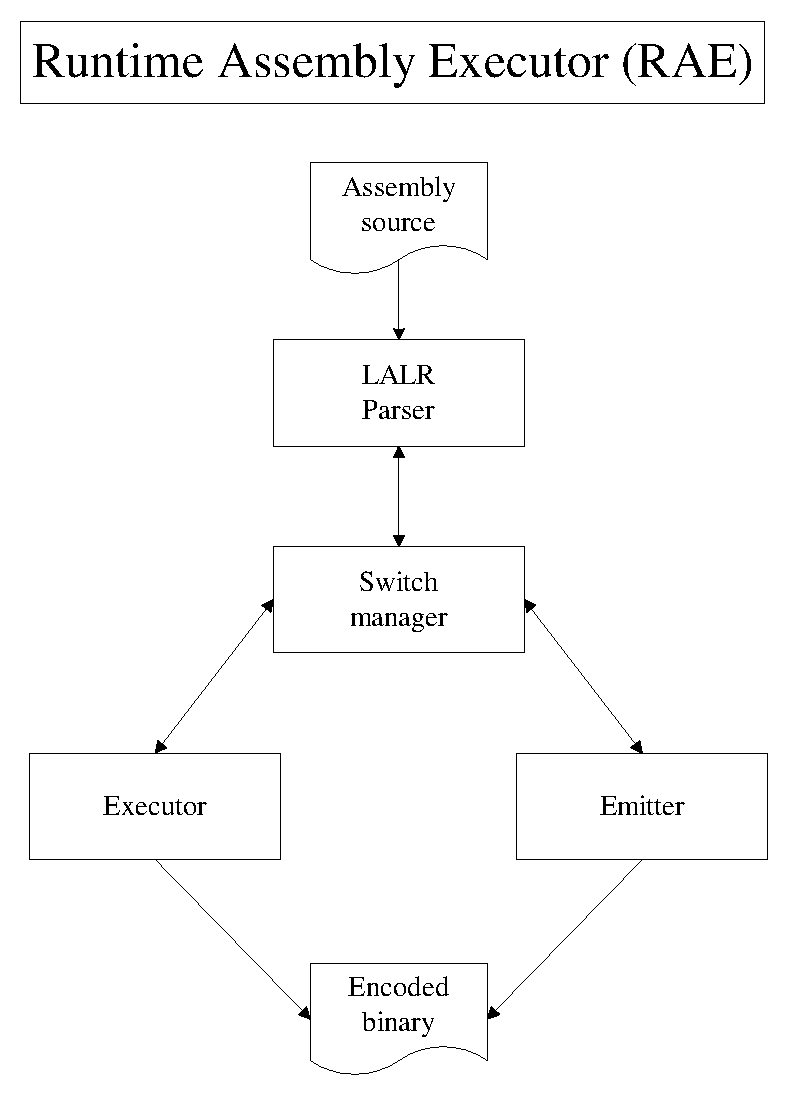
\includegraphics{figures/rae.eps}}
\centerfigend{fig-rae}{Components of RAE}

RAE is made up by 4 main components (see Figure~\ref{fig-rae}):  

\begin{itemize} 
\item 	The parser, 
		which parses VPO-generated assembly files using a LALR parser. 
		Structures, relocations, label information are gathered as each unit 
		of input is parsed.  Details regarding the parser are
		explained in more detail in the following subsections. 

\item 	The emitter, which uses NJMC toolkit encoding routines to encode the
		assembly instructions into binary instructions.  The emitter is invoked
		mainly by the parser and is reponsible for outputing the final binaries
		needed by the executor. 

\item 	The executor, which executes the translated binary code at run-time. 
	
\item 	The switch manager, which maintain the connections between the above
		components.  It jobs is to direct the flow of translation\/program 
		execution and the communications between the components such that 
		on-demand processing can be achieved.  
\end{itemize}

The dynamic behaviour of RAE results mainly from the ability to process
on-demand in the individual components.  Processing of each component are
done only when there is a need to do so.  For example, when the emitter
emits enough information for execution, the executor is invoked.  The
executor is then paused when there is a call to a label which it does not
yet know about, hence it invokes the parser to parse more source in search
for the desire label.  Each component are closely coupled in a way that
they are triggered on-demand.  Granularity of RAE can be seen as
processing one procedure at a time in the parser component. 


\section{RAE Parser} 
The parser is the first to be called by RAE.  
In a sequencial order, the parser starts at the top of the assembly file and
processes the input in an orderly fashion.  
The granularity unit of the parser is a single procedure at a time.  
The parser must gather enough information from the input file such that other
components can be invoked.  
During the parse, the parser invokes the emitter for every instruction that 
needs to be emitted.  
The combination of parsing and emitting pauses once the entry point to the 
main program is found in which the executor is called to execute the encoded
instructions.
Sometime during the running of the program, the switch manager may invoke the 
parser to parse more assembly input as needed.

Each procedure is consider to have a text segment and a local data segment.  
The first procedure
starting from the begining of the file and have no text segment.  It has a
single data segment which stores the labels that are accesible by the rest
of the program.  This is the only procedure that has no code segment and
it is the global data segment.  This segment is responsible to have names
and labels that are used throughout the rest of the program which are not
found in there local data segments.  Apart from being a single segment
procedure, this segment contains data that are similar to the rest of the
procedure's local data segments (at least in the eyes of the parser, they
are treated the same). 


\subsection{Data Segments} 

Data segments are static piece of memory that are allocated before the 
execution of the program.  
These segments may contains both initialised and uninitialised data.
Two types of data segments can be found in an assembly input file: 
texttt{global} and texttt{local} data segments.
The global data segment contains variables and label references that can be
accessed anywhere throughout the program.  
Contents within the local data segment are known only to its corresponding 
text segment.

\subsection *{Input to the parser}

The following assembly constructs are found in data segments within the input
file.

\begin{itemize} 
\item 	\texttt{.seg "data"} - this signifies the beginning of a data segment.
It is at this point that a new data relocatable block is created.  
Relocatable block are base structures provided by the NJMC toolkit. 

\item	\texttt{.align NUM} - NUM is usually 4, 8 or 16.  
a call to the align(NUM) routine is made whenever this is encoutered. 

\item	\texttt{.common VAR,SIZE,ALIGN} - variable VAR is declared with 
size SIZE, and its byte aligned to ALIGN.  
Call to align(ALIGN) is made first, VAR is added to the global symbol 
table if it have not been already added, SIZE bytes
is emited to the current relocatable block using emitm().  Since no
initial value is required, the emitter simply emits junk (currently set to
be the integer 2) for the .common identifier.  For example, in the
following variable declaration \\ \texttt{.common cm\_var, 1024, 4} \\ the
name \texttt{cm\_var} will be added to the symbol table with its offset
from the beggining of the global data segment.  The RAE then emits a
series of 1024 bytes with the value of 2 to specify that the address is
occupied through a series of calls to \texttt{emitm} (which handles
incrementing the \texttt{PC} counter and allocating space if the maximum
buffer space is reached). Another way to do this would be to call
\texttt{addlc()} which simply increments the \texttt{PC} counter. 
Although using \texttt{addlc()} is considerably quicker, extra code needs
to be added to performs similar housekeeping functions in \texttt{emitm}
like checking buffer overfloads if the relocatable block have just been
created.  addlc() can be safely used if a previous call the emitm() has
been made since the creation of the relocatable block.  If addlc() is the
first to be called after a new relocatable block, then some house keeping
is definately required. 

\item	\texttt{.global NAME} - signifies NAME is a global name that can 
be accessed anywhere in the program.  
NAME is added to the global symbol table and a
relocatable address for the NAME label is also created. 

\item	\texttt{LABEL:} - signifies a data label definition.  
If LABEL is not already in
the symols table (searches local symbols first then globals), it will be
added and a relocatable address is created aswell. 


The following belong within a LABEL 

\begin{itemize} 
\item .byte XXXX, 
\item .word XXXX, 
\item .double XXXX,
\item .ascii XXXX - the values XXXX associated with these tags are simply emited
to the current relocatable block. 
\end{itemize}

\end{itemize}

The input assembly file is generated from VPO, but its organisation
of data and text segments make it difficult for a single parse.  
For each text segment, there is always a corresponding local data segment 
(which could be empty).  
The organisation of the VPO assembly will start with the
global data segment, follow by the first text and local data segment pair,
then the second pair etc...  in that order.  Each pair of the text and
local segments is grouped as a single procedure by the parser.  Problem
with a single parse over the input file arises when encountering
references to local data variable its corresponding the text segment. 
Since its local data segment comes after its text segment, no reference
information about variables are known at the point of emiting an
instruction.  To overcome this problem, each local data segment could be
moved infront of its repectable text segment.  This can be very tedious
when the input file contains a large number of procedures.  To fixes this
problem, relocation closures are used.  Relocation closures are created
when an unknown symbol (or address) is referenced in the text segment. 
When the symbol is discovered (in its corresponding local segment), the
closure is applied to the instruction that created the relocation closure. 
This is done by patching the instruction space with the correct relocation
address. 

\subsection *{Example}

The following example code demonstrates the processing done during the
parse: 

input code:  
\begin{verbatim}
.seg "text"             (1)  
.align 8                (2)  
.global .L45            (3)  
.L45:                   (4) 
save %sp, -96, %sp      (5)  
sethi %hi(.L60), %o0    (6)  
add %o0, %lo(.L60), %o0 (7) 
...  
...  
.seg "data"             (8)  
.align 8                (9)  
.L60:                   (10)  
.word 0x46ff            (11)  
... 
\end{verbatim}

At the entry to the procedure, the parser allocates a new relocatable
block and does some housekeeping (1).  At (3), the symbol .L45 is added to
the global symbols table (global so that other procedures can call .L45). 
A label for .L45 is also created but not defined.  (4) defines label .L45
by assigning it the current offset from the beginning of the relocatable
block.  A save instruction is emited to the relocatable block by invoking
the respective emitter function (5).  As it encouters .L60 in (6), it
attempts to lookup the global symbols table in search for .L60 and fails. 
The parser adds .L60 to the local symbols table and creates a label for
it.  It then invokes the emitter which creates a relocation closure for
this instruction.  (7) uses .L60 again, this time the parser finds .L60 in
its local symbols and asks the emitter to emit the add instruction.  But
the emitter detects that .L60 is not defined and created another
relocation closure.  When the text segment is completed, the parser
creates another relocatable block for its local data segment(8).  At (10),
the parser defines .L60.  At (11), 0x46ff is emitted to the relocatable
block. 

As the RAE parser parses the VPO assembly output, it builds 2 (except the
first procedure) relocatable block for each procedure it encounters along
with a symbol table for all the symbols that are define in this procedure. 
When the parser finishes parsing a procedure, it tries to fix all the
incomplement instructions during the parse by applying the closures.  As
each closure is being appled, it patches over incomplete instruction with
the correct target address of the labels. 

Notice that the first procedure does not have a text segment.  This
procedure contains the global data section, hence the symbols table for
this procedure contains all the symbols and labels that are global to the
entire program.  This table defines variables that are accessible during
program execution. 

For succesful instruction encoding using global and local variable address
references and run-time execution, an exact copy of the disk image is
created in memory.  At the end of a procedure parse and after closures are
applied, information within each relocatable block are copied to a
contiguous piece of memory that is suitable for execution. 


\subsection{Text} 
As each procedure is being parsed, each assembly
instruction is determined, mapped and constructed by issuing a call to the
emmiter (see section 1.3) which invokes the corresponding NJMC encoding routine.  For example, for the assembly instruction 

\begin{verbatim}
	add %o0, 10, %o0 
\end{verbatim}

A call to the \texttt{add} function is made by the emitter to emit the
actual instruction to the text relocatable block. 

To process procedure call instructions, the parser looks up the global
symbol table and decides the next set of actions:  \begin{itemize} \item
For labels (infact, symbols as well) that are defined in the symbols
table, an explicit call instruction to the label's address is encoded. 
\item For labels not found in the table, the parser checks if the label
	exists in the libraries used by the program (currently only
	\texttt{libc.so.1} is checked). 
	If so, it is implemented as an indirected call.  Indirected calls
	are patched with two instructions---\texttt{sethi} and
\texttt{jmpl}. 
	The former instruction takes the address of the library routine,
	puts it into register \texttt{\%g5}, then a jump and link
(\texttt{jmpl})
	follows.  \item For unknown label, a call to the switch manager is
made.  The parser creates a new label for the destination of the call. 
Since the address of the destination is unknown at the time of encoding,
the
	name of the procedure that's being called is also passed to the
	switch manager. 
	See the section in On-demand to see how the switch manager is
used. \end{itemize}

The processing of branches is similar to that of calls for labels that
have been defined.  Branch targets that are unknown will result in
generating a relocation closure for the instruction with the target label
added to the local symbols table.  Branch target is never in the
libraries.

Closures are applied at the end of the parsing phase.  All fix ups within
intructions are handled by looping through the set of closures and
applying each in turn.  For address that are still undetermined during
closure analysis, the program will simply fail with an error.


\subsection{Others} In the case of loads and stores during the parsing of
the input file, the parser needs to indentify and encode the appropriate
instructions. Both version of float and integer loads uses the same
\texttt{ld} mnemonic but their opcodes are different.  The parser
determines whether the instruction involves floating point registers and
encodes the instruction accordingly---\texttt{ld} for integer loads and
\texttt{ldf} for floating point loads.


\section{RAE emitter} The RAE's emitter is automatically generated by the
NJMC tookit using the Sparc encoding specifications.  Communication
between the parser and the emitter is through the functions found in
\texttt{sparc.h}.  This file provides encoding functions that will
produces machine binaries for each Sparc instruction. 


\subsection{NJMC toolkit}

The NJMC toolkit can use a machine instruction specification to create
both encoding and decoding routine.  In this report, I will be discussing
encoding only.  The routines that can be used for encoding (as are used in
RAE) are generated by running xtools over the Sparc specification files. 
Function names are generated with relation to the names used in the spec
files.  eg. the add instruction will be implemented with the C function
ADD(rs1, reg\_or\_imm, rs2). 


\section{RAE executor} Control is parsed to the RAE executor with the
entry address of the main program.  The executor executed the encoded
instruction just like any other piece of code in memory.  The name of
executor is gcode, and its assign a value when the address of main is
found.  The executor is invoke by calling gcode() explicitly. 


\section{On-demand} One significant change from RAE rev 1 to rev 2 is the
introduction of on-demand processing.  On-demand processing allows
parsing, emiting and executing of code that are only requied at run-time. 

For each procedure parsed by the RAE parser, 2 relocatable blocks and 1
symbols table is constructed (except the first procedure).  The emitter is
invoked during the parse and actual instructions and data are emited
within the relocatable block.  At the end of a parse (end of one
procedure), all the relocation closures are apply.  Copies of each
relocatable to a contiguous piece of memory is done before the RAE parser
starts parsing another procedure. 

The RAE parser will parse the input file until the main procedure is
found.  Program execution start as soon as main is parsed and emited.  For
all other piece of code that are not yet parsed at this point in time, a
call to the "switch manager" is generated to take its place.  When a
program needs to call a procedure "proc1" yet to be parsed, instead it
calls the switch manager.  The switch manager looks up the list of
procedure that it knows about and tries to find "proc1".  If sucessful,
"proc1" is called.  If "proc1" does not exist in the known procedure list,
the switch manager asks the parser to parse another procedure until
"proc1"  is found and the code is emited.  When "proc1" is found, the
switch manager no only passes control to "proc1", it also patches the
original call to the switch manager with a call to "proc1". 

Example code before and after patching. 

original code to from input

\begin{verbatim}
add %o0, 0x188, %o0 
call proc1, 2 
add %o1, 0x302, %o1
\end{verbatim}

When call to "proc1" needs to be emited, the emitter emits a call to the
switch manager instead (instructions 0x60a70 and 0x60a74).  In order for
the switch manager to know that "proc1" is the required procedure, the
address containing the string "proc1" is also emited (instructions 0x60a68
and 0x60a6c). 

\begin{verbatim}
0x60a64 <_end+32108>:  add %o0, 0x188, %o0 
0x60a68 <_end+32112>:  sethi %hi(0x5bc00), %g5 
0x60a6c <_end+32116>:  add %g5, 0x258, %g5      ! 0x5be58 <_end+12640> 
0x60a70 <_end+32120>:  sethi %hi(0x13c00), %g6 
0x60a74 <_end+32124>:  call %g6 + 0x3b4         ! 0x13fb4 <switch_manager>
0x60a78 <_end+32128>:  add %o1, 0x302, %o1
\end{verbatim}

After the switch manager have found the address for "proc1" (through calls
to the parser and emitter in search for "proc1"), it patches the call to
the switch manager with a straight call to "proc1".  It also removes the
instructions at 0x60a68 and 0x60a6c. 

\begin{verbatim}
0x60a64 <_end+32108>:  add %o0, 0x188, %o0 
0x60a68 <_end+32112>:  nop
0x60a6c <_end+32116>:  nop 
0x60a70 <_end+32120>:  sethi %hi(0x62000), %g5
0x60a74 <_end+32124>:  call %g5 + 0x390 		! 0x62390 <_end+38552> 
0x60a78 <_end+32128>:  add %o1, 0x302, %o1
\end{verbatim}

Because the switch manager is do self modifying code, flush instructions
is needed to flush the cache such that it reflect what is now in memory. 
A jump to the procedure "proc1" is made at the end of the switch manage
			 % assembler encoder using the NJMCTK 


\part{Results}
\label{part-results}

	
\chapter{Results}
\label{ch-results}

{\small
\begin{flushright}
Documentation: Cristina, Mike [Sep 99]
\end{flushright}
}

This chapter provides current preliminary results in the use of
the \uqbt\ framework in 5 instantiations of the framework. 
The results were reported in 1999 at the Workshop on 
Binary Translation, Oct 99, and have not been updated since. 

After these results were reported, there has been progress
such that all the SPARC to SPARC and Pentium to SPARC tests in
the distribution file \texttt{test/regression.test} pass. Note 
that some of these passes are in fact rather forced---in some 
cases the generated C code is edited with a sed script. 
These are all due to limitations that we acknowledge, and which 
could be fixed if and when some things get implemented, such as 
endianness analysis for library function parameters. Of the Spec95 
integer benchmarks, only \texttt{compress} and \texttt{go} actually 
translate correctly, as far as we know, and only \texttt{compress} 
translates Pentium to SPARC. We have attempted to translate a few others, 
but it's tedious work due to lack of better debugging infrastructure. 
This illustrates the need for a debugging system, as discussed
elsewhere.

The following translators were used for experimentation and 
data collection: 

\begin{itemize}
\item uqbtss: static SPARC to SPARC
\item uqbtsp: static SPARC to Pentium
\item uqbtps: static Pentium to SPARC
\item uqbtpp: static Pentium to Pentium
\item uqbtsj: static SPARC to Java bytecode
\end{itemize}

A SPARC to SPARC and a Pentium to Pentium translators are useful
to test the adequacy of the internal representation, as translated
programs should not slow down when translating from machine M to 
machine M using the same optimizer compiler.  
Further, as seen in the results in this section, a binary translator 
can be used as an optimizer of binary code.  

The UQBT framework currently decodes and partially analyzes 
SPEC95 benchmark programs, such as compress, ijpeg, and gcc.
The largest of such programs is gcc with 1Mb of binary code (1.6Mb 
executable on SPARC and 1.2Mb on Pentium).
Our type analysis implementation is not complete, therefore we
currently only translate programs that take integer and pointer to
data parameters.
This limits the size of the programs that can currently be translated 
to the ones presented in Figure~\ref{fig-results}.
Further, our resourceable interpreter is not fully implemented yet,
hence we do not support programs that require runtime interpretation.
This has not been a problem for the programs presented herein, but
will be required for larger programs.

\begin{figure*}[htp]
{\small
\begin{minipage}[b]{\linewidth}
\begin{center}
\begin{tabular}{|r|r|r|r|r|} \hline
        & \multicolumn{2}{c|}{Translated Code} &
        \multicolumn{2}{c|}{Native Code} \\
Program & gcc opt & cc opt & -O0 & -O4 \\ \hline
Fibo(40) sec & 18.2  & 21.3 & 41.0  & 23.0 \\
       bytes & 24,924  & 6,700 & 24,628 & 24,564 \\ \hline
Sieve(3000) sec & 23.7 & 24.1 & 29.3 & 24.5 \\
       bytes & 24,732 & 6,316 & 24,552 & 24,452 \\ \hline
Mbanner(500K) sec & 25.8 & 22.2 & 63.7 & 26.6\\
       bytes & 30,500 & 12,248 & 30,652 & 30,268 \\ \hline
\end{tabular}
\end{center}
%\vspace*{0.1cm} 
\center{Static SPARC to SPARC Translation}
\end{minipage}\hfill
\vspace*{0.4cm}

\begin{minipage}[b]{\linewidth}
\begin{center}
\begin{tabular}{|r|r|r|r|r|} \hline
        & \multicolumn{2}{c|}{Translated Code} &
        \multicolumn{2}{c|}{Native Code} \\
Program & gcc opt & cc opt & -O0 & -O4 \\ \hline
Fibo(40) sec & 23.0 & 24.3 & 41.0 & 23.0 \\
       bytes & 24,916 & 6,680 & 24,628 & 24,564 \\ \hline
Sieve(3000) sec & 26.9 & 23.9 & 29.3 & 24.5 \\
       bytes & 24,776 & 6,312 & 24,552 & 24,452 \\ \hline
Mbanner(500K) sec & 53.3 & 36.9 & 63.7 & 26.6 \\
       bytes & 34,188 & 21,448 & 30,652 & 30,268 \\ \hline
\end{tabular}
\end{center}
%\vspace*{0.1cm} 
\center{Static Pentium to SPARC Translation}
\end{minipage}\hfill
\vspace*{0.4cm}

\begin{minipage}[b]{\linewidth}
\begin{center}
\begin{tabular}{|r|r|r|r|r|} \hline
        & \multicolumn{2}{c|}{Translated Code} &
        \multicolumn{2}{c|}{Native Code} \\
Program & gcc opt & cc opt & -O0 & -O4 \\ \hline
Fibo(40) sec & 27.7 & 28.5 & 28.6 & 25.9 \\
       bytes & 16,512 & 7,292 & 16,144 & 16,152 \\ \hline
Sieve(3000) sec & 17.8 & 17.4 & 18.9 & 18.6 \\
       bytes & 16,244 & 6,548 & 15,964 & 15,944 \\ \hline
Mbanner(500K) sec & 42.5 & n/a & 80.5 & 44.8 \\
       bytes & 22,240 & & 21,524 & 25,436 \\ \hline
%~\footnote{4,096 bytes added to executable to adjust data page size} \\ \hline
\end{tabular}
\end{center}
%\vspace*{0.1cm} 
\center{Static SPARC to Pentium Translation}
\end{minipage}\hfill
\vspace*{0.4cm}

\begin{minipage}[b]{\linewidth}
\begin{center}
\begin{tabular}{|r|r|r|r|r|} \hline
        & \multicolumn{2}{c|}{Translated Code} &
        \multicolumn{2}{c|}{Native Code} \\
Program & gcc opt & cc opt & -O0 & -O4 \\ \hline
Fibo(40) sec & 25.8 & 24.5 & 28.6 & 25.9 \\
       bytes & 16,496 & 7,268 & 16,144 & 16,152 \\ \hline
Sieve(3000) sec & 18.6 & 17.1 & 18.9 & 18.6 \\
       bytes & 16,228 & 6,536 & 15,964 & 15,944 \\ \hline
Mbanner(500K) sec & 48.7 & 46.5 & 80.5 & 44.8 \\
       bytes & 25,664 & 16,016 & 21,524 & 25,436 \\ \hline
%~\footnote{4,096 bytes added to executable to adjust data page size} \\ \hline
\end{tabular}
\end{center}
%\vspace*{0.1cm} 
\center{Static Pentium to Pentium Translation}
\end{minipage}\hfill
\vspace*{0.4cm}

%\begin{minipage}[b]{.46\linewidth}
%\begin{tabular}{|r|r|r|r|} \hline
%        & \multicolumn{1}{c|}{Generated Code} & 
%	\multicolumn{2}{c|}{Native Code} \\ 
%Program & Total & -O0 & -O4 \\ \hline
%Fibo(40) sec & 179.27 & 41.0 & 23.0 \\
%	byte & & 24,628 & 24,565 \\ \hline 
%Sieve(3000) sec & 83.00 & 29.3 & 24.5 \\
%	byte & & 24,552 & 24,452 \\ \hline 
%Mbanner(500K) sec & & & \\ 
%	byte & & & \\ \hline
%\end{tabular}
%\vspace*{0.1cm} \center{Dynamic SPARC to SPARC Translation}
%\end{minipage}\hfill
%\begin{minipage}[b]{.50\linewidth}
%\begin{tabular}{|r|r|r|r|r|r|} \hline
%        & \multicolumn{3}{c|}{Translated Code} & 
%        \multicolumn{2}{c|}{Native Code} \\
%Program & startup & dispatch & gen code & -O0 & -O4 \\ \hline
%Fibo(40) sec & 0.48 & 0.03 & 191.39 & 41.0 & 23.0 \\
%        bytes & & & 1,208 & 24,628 & 24,564 \\ \hline
%Sieve(3000) sec & 0.52 & 0.08 & 80.85 & 29.3 & 24.5 \\
%        bytes & & & 1,556 & 24,552 & 24,452 \\ \hline
%Mbanner(500K) sec & & & & & \\
%        bytes & & & & & \\ \hline
%\end{tabular}
%\vspace*{0.1cm} \center{Dynamic Pentium to SPARC Translation}
%\end{minipage}\hfill
%\vspace*{0.4cm}
%
%\begin{minipage}[b]{.42\linewidth}
\begin{minipage}[b]{\linewidth}
\begin{center}
\begin{tabular}{|r|r|r|r|r|} \hline
        & \multicolumn{2}{c|}{Translated Code} & 
        \multicolumn{2}{c|}{Native Code} \\
Program & Interpreter & JIT & -O0 & -O4 \\ \hline
Fibo(40) sec & 421.64 & 58.02 & 41.0 & 23.0 \\  
	bytes & 739 & 739 & 24,628 & 24,565 \\ \hline  
Sieve(3000) sec & 103.66 & 20.52 & 29.3 & 24.5 \\ 
	bytes & 677 & 677 & 24,552 & 24,452 \\ \hline
%Mbanner(500K) sec & & 10m16.06 & 22.11 & 10.01 \\ 
% 	bytes & & & & \\ \hline
\end{tabular}
\end{center}
%\vspace*{0.1cm} 
\center{Static SPARC to Java Bytecode Translation}
\end{minipage}\hfill
%\begin{minipage}[b]{.46\linewidth}
%\begin{tabular}{|r|r|r|r|r|} \hline
%         & \multicolumn{2}{c|}{Generated Code} & 
%         \multicolumn{2}{c|}{Native Code} \\
%Program & interpreted & JIT & -O0 & -O4 \\ \hline
%Fibo(40) sec & & & & \\  
% 	bytes & & & & \\ \hline  
%Sieve(3000) sec & & & & \\
% 	bytes & & & &  \\ \hline
%MBanner(500K) sec & & & & \\ 
% 	bytes & & & & \\ \hline
%\end{tabular}
%\vspace*{0.1cm} \center{Static Pentium to Java Bytecode Translation}
%\end{minipage}\hfill

\label{fig-results} \caption{Running Times and Code Sizes for Static
	Translators Instantiated from the UQBT Framework}
}
\end{figure*}

%%Figure~\ref{fig-results} presents results for 6 different
%%Figure~7 presents results for 5 different instantiations of the UQBT 
Figure~\ref{fig-results} presents results for 5 different instantiations of 
the UQBT framework.  The test programs are: 

\begin{itemize}
\item Fibo(40), which calculates the fibonacci of 40 and has 63 lines 
of assembly code, 
\item Sieve(3000), which calculates the first 3000 primes and has 
61 lines of assembly code, and
\item Mbanner(500K), a modified version of banner(1), which loops 
500,000 times to display argv[1] (``1234567890'' in this case) and 
has 204 lines of assembly code and a read-only data section 
of 336 bytes.
\end{itemize}

For all programs, we measured the time in seconds to execute
the program on the target machine and compared that to the
time measurement produced by a native compiler on that target
machine; this allows us to see the quality of the translation.
Each test program also lists on the second row the size in bytes
of the executable file for comparison purposes.
SPARC results were obtained on an UltraSPARC II, 250MHz machine
with 320Mb RAM running Solaris 2.6.
Pentium results were obtained on a Pentium MMX, 250 MHz machine
with 128Mb RAM running Solaris 2.6.
The source binary programs (input to the translator) were all compiled 
with gcc 2.8.1 -O4.  
Translated code programs used two different optimizing C 
compilers; gcc 2.8.1 and cc 4.2, on both SPARC and Pentium machines. 
Native code for the target machine was compiled using gcc 2.8.1
with -O0 and -O4 options, on both SPARC and Pentium.  
%%Results for -O0 are included to indicate how much variation optimization 
%%causes on the source architecture. 

As can be seen from the results, the statically translated code is just 
as efficient as native code on translations across the same 
architecture (i.e. SPARC to SPARC and Pentium to Pentium), 
and small or negligible overhead is created on static register-based
translations across different architecture machines.
This is due to the abstraction of code into \hrtl\ code 
and perhaps the small size of the test programs, which do not 
necessarily test all the features of large programs 
(such as differences in types or the need for interpretation).
Some translated programs (those translated by uqbtss and uqbtpp) are 
faster than their native counterparts because of accidents of instruction 
scheduling.  We compared the input and the translated program and 
noticed a few extra nop's and unfilled delay slots in the input 
optimized binaries.  These can make a very large difference for 
programs like fibonacci, which have very short inner loops doing most of 
the work.

The version of Sieve that is translated from the Pentium to the 
SPARC runs 9\% slower than the version compiled from C source 
code by the native SPARC compiler, when using gcc as the optimizer 
with UQBT. Because the Pentium has fewer registers than SPARC, 
the Pentium compiler did not put all variables in registers. 
In the translation from the Pentium binary, those variables remain
in memory, but when the native SPARC compiler translates the same
source code, it puts all variables in registers, so the natively 
compiled version is 9\% faster.  In contrast, the cc optimizer does  
perform this optimization and the result is a generated binary 
that runs at the same speed as native code.  

Translations between machines of different endianness, such as 
SPARC and Pentium, may require the use of byte swapping at each load 
and store in order to access initialized data.  This is the case
of the Mbanner Pentium to SPARC static translation, where a 100\%
overhead is seen.  
This is due to two main factors: memory locations are not promoted 
to registers wherever possible, and there are redundant byte swaps 
due to endianness differences.
In our translation to SPARC, the machine has to 
perform costly byte swapping for one 32-bit load instruction, which 
results in 10 SPARC instructions.  
Two redundant 32-bit byte swaps result in 20 SPARC instructions 
which the optimizer cannot remove.  This problem is not seen in 
SPARC to Pentium static translations however, because the Pentium has 
a single instruction to perform 32-bit byte swapping. 
The two shortcomings identified in the generated code can be 
rectified by implementing binary translation-specific optimizations 
at the \hrtl\ level, before emitting machine-dependent code.  

The Pentium to SPARC translations suffer a large performance hit
because of the way that endianness swaps are implemented. The
cost is some 8 SPARC instructions, with an extra 2 for the first
one (and if the register used to hold the mask is re-used). Most
SPARC machines these days have UltraSparc processors, and with
these machines it is possible to perform endianness swaps during
loads and stores (alternate address space 0x88 performs the
required swapping).

To implement the alternate address scheme, the macros need to be
split into two groups; one for loads, and one for stores. (Both
of these would be almost the same for Pentium targets). Also,
there is the issue that for the lowest overhead, two different
assembly language forms have to be used; one for when the SPARC
addressing mode is register plus register, and one for when it is
register plus constant. We did not implement these changes, 
so regrettably we do not know what the true cost of translation
from Pentium to SPARC really is (i.e. at present, it is
needlessly being swamped by the cost of endianness swaps using the 
first-mentioned method).

For the translator of SPARC to Java bytecodes we show 
initial results obtained without having performed stack-based 
optimizations on the code.  
Nevertheless, the JIT compiled 
version compares favourably with native code on the SPARC, 
especially due to the efficiency of present JIT compilers, 
which translate two or three bytecode instruction sequences 
into one target native instruction. 
These results apply to small integer benchmarks. 

      % results on performance of gen'd binaries

	
\chapter{Instantiation of Translators}
\label{ch-instantiation} 

{\small
\begin{flushright}
Design: Cristina; Documentation: Cristina [Apr 01]
\end{flushright}
}


This document is based on the experience gained by the 
UQBT team in instantiating binary translators out of the UQBT framework.  
The following translators have served as test beds for the 
development of this process: 

\begin{itemize}
\item SPARC to Pentium
\item Pentium to SPARC
\item MC68000 to MC68000
\item PA-RISC to SPARC 
\end{itemize}

The UQBT framework, described in Chapter~\ref{ch-uqbt-framework} 
and replicated below in Figure~\ref{fig-uqbt-framework}, provides 
the basis for a step-wise process of instantiating modules out of
the framework.  

\psfigbegin{figures/uqbtImplementation.eps}{10cm}
\psfigend{fig-uqbt-framework}{The UQBT Framework}

In order to instantiate a new translator, the APIs and specification 
files for the source platform need to be described. 
The output of the module that services each API or specification is 
tested in order to ensure correctness of the intermediate output.  

The instantiation process consists of the following steps: 
\begin{enumerate}
\item Binary-file decoder support

\item Instruction decoding support 

\item Instruction semantics support

\item Control transfer support

\item Procedural abstraction support

\item Machine-specific support

\item Code generation support
\end{enumerate}

Each step is described in some detail in the following sections.
Throughout this presentation, the steps have been divided into 
the three logical parts of the translator, that is, instantiating
a front-end, instantiating to HRTL level, and instantiating
a back-end.


\section{Instantiating a New Front-end}
In order to support a new front-end for a machine M$_s$, we 
need to provide support for the binary-file format in which 
the executable file is stored in, as well as the syntax and 
semantics of the machine M$_s$ instructions.  

\subsection{Binary-file Decoder Support}
In order to support different binary-file formats, such as 
ELF, PE, PRC, etc, UQBT exports a loader API called 
\texttt{BinaryFile}.  \texttt{BinaryFile} is an abstract class 
that makes available functions to:

\begin{itemize}
\item construct, load and unload binary files, 
\item extract information from sections, 
\item extract information from symbol tables (if any), 
\item extract information from relocation tables (if any),
\item display/dump the contents of all headers, and 
\item obtain initial program state information, such as entry 
	point(s), and determine whether a given address is a dynamically-linked 
	address or not.  
\end{itemize}

For a given binary-file format BFF$_i$, the \texttt{BinaryFile} 
API is satisfied by implementing the derived BFF$_i$BinaryFile 
class.  In this class, some extra functions are used to 
implement the \texttt{BinaryFile} interface, depending on 
the complexity of implementing the API functionality.  

Testing of this step is done by displaying/dumping to the screen 
the contents of all headers and sections read from the file. 
This contents is then checked manually against the contents 
produced by a binary-file dump tool, commonly distributed with
operating systems these days.  For example, under Unix, the  
\texttt{elfdump} tool displays the contents of an ELF's file 
headers.  A typical size of information dumped is around 500 
lines of ascii text.  Similar results are achieved by using 
GNU's \texttt{objdump} tool. 

Modules to bring across from the UQBT source code (we use the
following command: \texttt{cvs co -N -d . uqbt/dirName} 
and then rename the \texttt{uqbt} directory to a suitable 
name): 
\begin{itemize}
\item The \texttt{uqbt/loader} directory and all its files
\item The \texttt{uqbt/include} directory and all its files
\item The driver and Makefile for the bffDump program 
	(\texttt{uqbt/loader/bffDump}); these programs 
	need to be placed at top level. 
\end{itemize}

The skeleton file \texttt{bffDump.cc} provides the basis 
for creating a binary-file dumper, also known by others as object 
dumper, which displays the raw contents of each of the headers and 
fields of the given binary-file.

The \texttt{BinaryFile::DisplayDetails} function needs to be overridden 
and implement the displaying of the BFF's header, its program 
header and section headers, as well as the information within 
those sections. 

Using \texttt{elfdump} on Solaris, the following options 
show parts of the Elf file; invoking \texttt{elfdump} with 
a file name displays all the section information in the file. 
Options (from the man page): 
\begin{itemize}
\item \texttt{-e}: dump the elf header,
\item \texttt{-p}: dump the program headers, 
\item \texttt{-c}: dump section header information,
\item \texttt{-d}: dump the contents of the .dynamic section,
\item \texttt{-s}: dump the contents of the symbol table sections (that
           is, .dynsym and/or .symtab).
\end{itemize}

Testing against a tool like \texttt{objdump} requires different
options to be set in order to see different parts of the file: 
\begin{itemize}
\item \texttt{--file-headers}: displays the Elf header
\item \texttt{--section-headers}: displays the section headers 
\item \texttt{--headers}: displays the section headers only (it 
	does not include the program headers)
\item \texttt{--syms}: displays the contents of the symbol table
\item \texttt{--dynamic-syms}: displays the contents of the dynamic symbol 
	table
\item \texttt{--all-headers}: displays all section headers and the 
	contents of the symbol table.
\end{itemize}


\subsection{Instruction Decoding Support}
	This is the most time consuming step in the process as the 
	binary translator writer needs to become fully familiar with 
	the instruction set to be supported.  This step involves 
	reading through architecture manuals and representing the 
	information for instructions in terms of the SLED language. 
	SLED allows for the description of the types of instructions 
	in a given machine, the fields of such instructions, the 
	values of particular fields of instructions, and the description
	of what individual instructions are, in essence, allowing for
	the mapping of binary bit streams to assembler instructions. 
	In our experience, depending on how complex the instruction 
	set is, and how familiar the writer is with the instruction 
	set, this step can take anywhere from 2 weeks to 2 months. 

    The New Jersey Machine Code toolkit (NJMCTK) not only supports 
	the SLED language, but also supports an abstraction to decode and 
	encode machine instructions.  The decoding abstraction provides for
    a \emph{matching} statement whose syntax resembles that of
    a C switch statement, and whose semantics is equivalent to
    matching the series of bits that form an instruction and
    returning the values of the variable fields of an instruction.
    In this way, a decoder (disassembler) of machine instructions 
	can be written, and the time to do this is minimal (less than 
	1 day), in fact, it is possible to automatically generate such
	a decoder.  This decoder is tested against an existing 
	disassembler for the source machine through a series of test 
	cases.  This is possible as most Unix systems include a \emph{dis} 
	utility in their distribution or one is included as part of 
	the GNU \emph{binutils}.

The following files/directories need to be downloaded: 
\begin{itemize}
\item \texttt{uqbt/loader}
\item \texttt{uqbt/include}
\item \texttt{uqbt/machine}
\item \texttt{uqbt/disasm} and put the files 
	from this directory at top level (disasm.cc, disassembler.m, mltk.sh 
	and Makefile)
\item rename directory \texttt{uqbt} to something else (e.g.
	\texttt{disasm})
\end{itemize}

Write the SLED spec for the architecture of choice.  
New machine descriptions are to be placed in the 
\texttt{machine/machineName} directory. 
Write a decoder based on the spec; sample decoders are given 
in the machine directory; for example, the 
\texttt{machine/sparc/disassembler.m} 
file is the decoder for the SPARC. 

The decoder to be written is a ``matching'' file, which gets 
processed by the New Jersey Machine Code toolkit (NJMCTK), along
with the SLED spec, into a C++ file which performs the matching
of bits to instructions.  
For information on SLED specifications refer to Ramsey and 
Fern\'{a}ndez~\cite{Rams97} and Chapter~\ref{ch-decoding} of 
this documentation.  

Appendix~\ref{ch-config} contains notes on how to configure
UQBT to generate disassemblers. 


\subsection{Instruction Semantics Support}
	The writing of the SSL spec is not too hard to do once the 
	SLED spec has been written, basically because by then the 
	writer is very familiar with the instruction set being 
	described.  In our experience, writing the SSL spec takes 
	less than one third of the time that it takes to write the
	SLED spec.  

	Our current testing of the SSL spec is in terms of an extension
	to the decoder.  Instead of the decoder dumping raw assembly 
	information, it dumps RTL information.  Such information is 
	manually tested against the assembly output. 

In the decoder file, you need to add support to return semantic
strings rather than plain strings.  Further, an extra function 
will be needed to cater with numbers and predefined register 
names (e.g. dis\_Reg() and dis\_Num()). 

Except for the PA-RISC, all other CISC and RISC architectures we have 
dealt with were almost straight forward supported by SSL.  However, 
in the case of PA-RISC, a more expressive language was needed in order 
to support pre and post semantics of instructions based on bits of 
an instruction.  This mean that an extension to the language was 
done and it took far longer than expected.   


\section{Instantiating to HRTL Level}
The M$_s$-RTL to \hrtl\ translator is composed of support for 
control transfer instructions, procedural information, and 
any extra code to support source machine-specific details. 

\subsection{Control Transfer Support}
	The New Jersey Machine Code toolkit (NJMCTK) supports the 
	SLED language as well as an abstraction to decode and encode 
	machine instructions.  The decoding abstraction provides for 
	a \emph{matching} statement whose syntax resembles that of 
	a C switch statement, and whose semantics is equivalent to 
	matching the series of bits that form an instruction and 
	returning the values of the variable fields of an instruction.
	In this way, a decoder of machine instructions can be written. 
	The support for the control transfer API is in terms of 
	extra instructions that get added to this matching driver 
	statement, so that control transfer information gets 
	encoded into the decoded $M_s$-RTLs.    	

	This API is very loose and not formally specified per se, 
	though it is hardcoded into the code.  The M$_s$-RTL instructions
	to which control transfer support has been applied, are an 
	``in between'' RTL form that we call IRTL.  IRTL stands for 
	``independent RTL'', and they resemble HRTL instructions, 
	with the exception that their operands have not been obtained 
	yet (these are obtained through procedural abstraction 
	recovery). 

	This step is almost trivial and can be implemented in 1 day 
	after looking at skeletons of existing translators. 

\subsection{Procedural Abstraction Support}
    The PAL spec is based on the operating system ABI conventions
    for setting up the call stack frame, parameter passing and
    calling conventions.  Specifying this information takes
    little time (2 days) once the information to be specified has
    been determined.  

    Testing of the PAL spec is done by compilation into the
    source binary form.  In this way, a translator of mc68328 Palm
    to mc68328 Palm binaries is instantiated for testing purposes.
    We test the SSL and PAL specs by determining if the translated
    programs behave in the same way as the original program.
    In our experience, we do not introduce performance degradation,
    in fact, the generated binaries compare favourably to native
    code geneated on the target machine, and in some cases it
    performs faster (due to optimization choices).  However, before
	being able to perform this test, the next step may need to 
	be applied. 

	Programs do not necessarily only adhere to the OS' ABI calling 
	conventions, therefore, some of the calling conventions that 
	we have included in PAL specs have been determined by trail and 
	error, after testing a program that does not adhere to the 
	ABI conventions.  We normally just include the new convention in
	the PAL spec. 

\subsection{Machine-specific Support}
	Add any extra analysis that is too machine-specific: 
	In order to remove all the peculiarities of a given source 
	machine, there may be need for an extra analysis to be added. 

	In our experience, each machine has a particular peculiarity 
	that is too machine-specific to be supported in the framework. 
	For example, SPARC has delayed transfers of control, x86 has 
	a stack-based representation for their floating point instructions, 
	mc68k makes use of a data pointer as a global pointer into data, 
	etc.  We normally try to address these issues in a fairly 
	generic way, though it is not always necessary to solve them 
	in that way.  In the case of delayed transfers of control, our 
	generic solution has been useful for reusing it for PA-RISC 
	code.  


\section{Instantiating a New Back-end}
Throughout the last few years, the UQBT's back-end has interfaced 
to a C compiler in order to optimize the intermediate code 
generated by UQBT.  In that framework, HRTL code is translated
to low-level C code, effectively using the C compiler as an 
assembler.  
We are now extending the framework to integrate with existing 
retargetable optimizers at the RTL level.  In this way, HRTL 
code is translated to $M_t$-RTL code and fed into an optimizer
such as VPO~\cite{Beni88} using the new VPO interfaces from the
Zephyr project~\cite{Vpo98}.  
Figure~\ref{fig-newUqbt} illustrates the new UQBT framework.  

\psfigbegin{figures/uqbtOverall2001.eps}{10cm}
\psfigend{fig-newUqbt}{The 2001 UQBT Framework}

In order to generate $M_t$-RTL code we need to solve several 
problems that are not discussed in this paper; these are: 
\begin{itemize}
\item Transform HRTL code to $M_t$-RTL code in a machine-independent way. 
      This step requires a few extensions to the PAL language in 
      order to support code generation of procedure call information 
      in a retargetable way, for example, by being able to use 
      specified calling conventions and parameter passing conventions, 
      as well as being able to set up the stack frame in the way expected
      in the target machine. 

\item Satisfy the $M_t$-RTL invariant that some optimizers require. 
      This invariant basically asks for an RTL to be equivalent to 
      an assembly instruction in the target machine.  This invariant 
      allows retargetable optimizers to perform not only machine-independent 
      optimizations but also machine-dependent ones. 
\end{itemize}


\subsection*{Translation via low-level C}
The C code generator back-end generates low-level C code, effectively
using the C language as a macro assembler.  Figure~\ref{fig-cgen-eg} 
shows the code generated by this back-end for the sample program. 
As can be seen from the code, type casting is used very often  
due to the need to ensure that the C compiler does not infer different
semantics to the one expected.  

\centerfigbegin
\begin{fnverbatim}
#include "uqbt.h"
void proc1(int16 v0, int32 v1, int16 v2) {
	int16 v3;
	int32 v4;
	int16 v5;
	int16 v6;
	int16 v7;
	int16 v8;
	int32 r3, r4, r5, r8;
	int32 temp1;
	int32 tmp1;
	/* 3c6 */

	*(int16*)&r5=v0;
	*(int16*)&r4=v2;
	temp1= *(int16*)&r4;
	v5=temp1;
	v4=33566720;
	v3=proc3(v4,v5);
	temp1=v3;
	*(int16*)&r3=temp1;
	tmp1=(unsigned int16)( *(unsigned int16*)&r3);
	v6=tmp1;
	if ((*(int32*)&v6)==(0)) goto L1;
	temp1=(int32)( *(int16*)&r3);
	r8=temp1;
	temp1=r8;
	*(int32*)&v3=temp1;
	goto L2;
L1:		/* 3f0 */
	temp1= *(int16*)&r5;
	v3=temp1;
	v7=v3;
	if ((*(int32*)&v7)==(0)) goto L3;
	goto L4;
L3:		/* 3f6 */
	v3=proc2();
	temp1=v3;
	 *(int16*)&r3=temp1;
	tmp1=(unsigned int16)( *(unsigned int16*)&r3);
	v8=tmp1;
	if ((*(int32*)&v8)==(0)) goto L5;
	temp1=(int32)( *(int16*)&r3);
	r8=temp1;
	temp1=r8;
	*(int32*)&v3=temp1;
	goto L2;
L5:		/* 406 */
	v5=1000;
	FrmGotoForm(v5);
	proc4();
	proc5();
L4:		/* 418 */
	*(int32*)&v3=0;
L2:		/* 41a */
	return;
}
\end{fnverbatim}
\centerfigend{fig-cgen-eg}{Generated C code for the example in Figure~\ref{fig-hrtl-eg}}


\subsection{Translation via RTL code} 
Please refer to documentation in Chapter~\ref{ch-vpobackend}. 


\subsection{Translation to JVML code}

Translators to bytecode require extra environment support
to compliment the strengths of the JVM.  The lack of a generic memory
model on the JVM forces us to emulate the data and stack of a translated
program.  Library functions from the source architecture must also be
supplied to the translated program.  This is facilitated by a superclass
from which each translated program is inherited.  The superclass provides
simulated memory access in preloaded byte arrays and wrapper routines to 
library functions which invoke the native Java subsystems.

For more information, please refer to Chapter~\ref{ch-jvm}. 

 % instantation process to generate new translators

	%
% Sep 99: Cristina, created, based on WBT paper
% Sep 01: Cristina, updated, based on Palm experiments from Mar 00 
%            and writeup from May 01 
%

\chapter{Experience in the Use of the UQBT Framework}
\label{ch-experience}

{\small
\begin{flushright}
Documentation: Cristina [Sep 99, Sep 01], Mike
\end{flushright}
}

This chapter documents our experiences in building the \uqbt\ 
framework, and ours and others experiences in the use of the 
framework to instantiate translators. 
Our experiences in building the framework are described in terms of 
effort to create the \uqbt\ framework itself and effort in instantiating 
a new frontend or a new backend.  The adaptability of the framework 
is shown through the support for other architectures. 
The core of this chapter was written in 1999, the Palm experiences 
were written in 2001.  

As reported in the Instantiation chapter (Chapter~\ref{ch-instantiation}), 
writing a new frontend requires the SLED, SSL and PAL specifications 
to be written, as well as the binary-file format and the control-transfer
APIs to be satisfied.  Further, any machine-specific information that is 
not supported directly by the framework needs to be coded in as part of
the RTL to HRTL translation step.  
When writing a new backend, experimentation is mainly with different 
ways of generating code (at different levels of abstraction) in order
to try out a different optimzizer (say VPO or the PostOptimizer).  


\section{Effort in Building the UQBT Framework}
The UQBT framework provides binary translation writers with 
support for new architectures at low cost.  
This is evidenced by the effort to support a new architecture,  
which is low because most of the UQBT framework is reused. 
We quantify the effort to develop the UQBT environment and 
the effort to reuse it.  
We also provide our experiences with supporting a new target 
architecture, a stack-based architecture in this case.


\subsection{Development of the Framework}
The development of the UQBT framework has been an order of 
magnitude larger than writing a hand-crafted binary translator 
from scratch.  This complexity was introduced by the need to 
make the framework re-sourceable in particular, and the 
need to separate machine-dependent concerns from machine-independent
analyses.  UQBT has been developed over a period of 4 years 
by a small team, consuming 6.2 person-years (some of those with 
relatively inexperienced students initially).   
%% CC: it's 6.2 man-years w/o the JVM, which is 0.5 and it's 
%% mentioned elsewhere.  I've made these figures til end of Dec. 
%% In my time, I didn't include all this writing up of papers, 
%% which has consumed a fair bit while I've been here. 
%% Breakdown of 6.2 man-years: [at eoDec 99]
% Mike: 3 years * 80%
% Cristina: 3.5 years * 50% + 0.5 years * 30%
% Shane Sendall: 1 * 40% (SSL) 
% Doug Simon: 1 * 50% (SSL, PAL) 
% David Ung: 1 * 100% (SSL)
%% JVM back end: Trent Waddington: 1 * 50% (JVM) 
%% for dynamic, David Ung, extra 2 years * 100%

The use of specifications allows us to create new binary translators 
quickly, by instantiating from the UQBT framework by specifying the 
source and target machine, reusing most of the components in the system 
and providing a driver skeleton for the decoding phase.  
In order to support peculiarities of particular machines, extensions 
to the system may be required, either in the form of extra analyses 
(specific to one machine) or extra constructs in the semantic 
language. 

To add DCTL support we expect a 0.2 person-year effort as this is 
a simple transformational language which is easily described 
and used.  DCTL can replace about 1000 lines of code, which are currently 
specific to the SPARC architecture.  Due to the low occurrence
of the delayed transfer of control concept on modern architectures, 
we have not placed a high priority in the implementation of this language.  


\subsection{Reuse of the Framework---Low Cost}
The size of the specifications gives an estimate of the amount 
of code a developer would need to write in order to get 
the basic translation system to work, or in determining how 
much it supports a given pair of machines.  
Current machine instruction descriptions (syntax, semantics, 
control flow) for SPARC and Pentium architectures are between 1,100 
and 2,600 lines, and calling convention and stack frame specifications 
are around 200 lines each (see Figure~\ref{fig-specSizes}.
This is in contrast to 26,500 lines of source code, 
6,200 lines of definitions in header files, 
3,900 lines of specification files and the 
skeleton driver generated by the framework (on average 2,000 lines).  

\centerfigbegin
\begin{tabular}{|l|c|c|c|} \hline
Machine & SLED & SSL & PAL \\ \hline
SPARC & 306 & 689 & 173 \\
Pentium & 746 & 1626 & 172 \\
mc68K & & & \\ \hline
\end{tabular}
\centerfigend{fig-specSizes}{Number of Lines of Code for Different
    Machine Specs.}

This highlights the reduced amount of code that a binary 
translation writer would have to develop.  Further, reuse of
specifications is also possible, particularly when other 
people have already written such specifications.


\subsection{Endianness}
\emph{This section needs to be updated.} 

Without special analysis, it is necessary for the translated program to run
using the endianness of the source program. This basically implies swapping the
byte ordering of multi-byte memory references after every load and before every
store. The Pentium processor has single instructions for doing this, but the
sequence on the SPARC is 10 instructions for the first swap, and 8 instructions
thereafter if a constant mask can be retained in a register.

For memory intensive programs, this overhead can be quite large, and in the
case of a SPARC target, there is additional register pressure as well
(i.e. a variable that might have otherwise been optimized to registers
will have to be spilled to memory).  Further, in the context of
byte swapping, instructions like ``increment memory variable'', that
require 5 \hrtl\ instructions:

\begin{smallverbatim}
  v1 = m[%afp + 4]
  byteswap (v1)
  v1 = v1 + 1
  byteswap (v1)
  m[%afp + 4] = v1
\end{smallverbatim}

end up being represented in SPARC machine code as a series of up to 21
instructions: 1 instruction for the memory load, 8 or 10 instructions for the
first byte swap, 1 instruction for the increment, 8 instructions for the
second byte swap, and 1 last instruction for the memory store.
This type of code cannot be optimized by even the best current
optimizers.

In the generated code, some of the byte swaps are redundant or could
be eliminated with analysis, in effect removing the overhead created
on machines that do not natively support byte swapping of words.
In the UQBT framework, this analysis can be done at the \hrtl\ level, 
but such analysis has not been implemented at this point in time.


\section{Experiences with Translation to Bytecodes of the Java Platform}
The adaptability of the UQBT framework was first tested in 1999 by our 
student Trent Waddington by supporting translations to bytecodes, the 
assembly language of the Java virtual machine. 
We instantiated two new translators, \texttt{uqbtsb} and \texttt{uqbtpb}, 
to translate from SPARC and Pentium architecture binaries to bytecodes. 
We reused the specifications for the source machines and 
wrote a back end for \texttt{gcc} (the GNU C compiler) to generate 
bytecodes in assembly files linkable by \texttt{jasmin}~\cite{Meye97} 
into Java class files. 

In order to run bytecode binaries, an extra support environment 
was written to provide support for memory access and pointers 
to memory, as well as translating some library calls.

The results of this experiment were good.  The performance of 
the translated programs on non-memory intensive micro-benchmarks 
were comparable to native C code compiled on the machine where the 
JVM was running.  Memory intensive programs showed a performance 
degradation due to our memory management support and to the 
lack of unsigned integral types in the JVM.   

The overall effort of this experiment was 0.5 person-years in 
the development of the \texttt{gcc} JVM back end, the JVM runtime 
support environment, and testing of micro benchmarks. 
 

\section{Experiences in Instantiating a Palm Translator} 
One of the advantages of a retargetable framework is that it 
allows the framework to be used in unexpected ways.
Our experiments translating PDA applications illustrate this flexibility
as the framework was not specifically designed for translations 
of embedded systems software.

We experimented with translating CISC mc68328 Palm applications to a 
RISC processor, the ARM, as well as to bytecodes for the
Spotless~\cite{Taiv99} virtual machine for the Java platform.
Spotless is Sun Microsystems Laboratories' virtual machine for small 
devices that runs on PalmOS.
A commercial version of Spotless that is independent of PalmOS
is available as the K virtual machine\TM (KVM\TM).
The KVM runs on multiple platforms including the Palm.

We instantiated two translators:
one from the (mc68328,PalmOS) to the (ARM,PalmOS) 
and the other from (mc68328,PalmOS) to the (Spotless,PalmOS).
We use the term ``instantiated''
because the work of creating a new translator
often consists of selecting among existing components
rather than implementing an entirely new translator from scratch.
We also use a (processor,operating system) notation
to describe more precisely a specific platform:
a combination of a processor and an operating system.
The first section below describes how we instantiated the
mc68328-to-HRTL front end shared by both translators.
The next two sections describe the use of two UQBT back ends
to generate, respectively, ARM machine code and JVM bytecodes.

This experiment was run by Cristina and Mike in March-May 2000. 
We mainly worked on instantiating a new mc68328 frontend, which 
took some time due to lack of familiarity with the mc68328 
architecture.  We were familiar with the SLED, SSL and PAL 
description languages, as well as how the \uqbt\ framework works. 
In Feb 2001, Brian Lewis run experiments with existing backends, 
the low-level C and the JVM backends.  
A total of 3.5 man-months was spent in the experiments reported 
herein. 


\subsection{Instantiating a UQBT front end for mc68328 Palm binaries}
The first step in instantiating a new translator
is to build a front end for the source platform.
The front end translates source binary files
into the HRTL intermediate format.
This requires writing, or reusing, SLED, SSL and PAL specifications
for the source platform.
Also, an implementation of the binary file API for the
source binary files must be available.
If one does not already exist, it will have to be written.
This process is explained in detail elsewhere (Chapter~\ref{ch-instantiation}).
We give an overview of the steps involved here
as well as the effort involved for those steps when
instantiating the (mc68328,PalmOS) translators.
In brief, the steps involved in instantiating the framework are:

\begin{itemize}
\item Write support for the binary file format:
%\textbf{Write support for the binary file format:}
        The PalmOS uses .PRC files, which were not yet supported by UQBT,
	so we wrote a \texttt{PalmBinaryFile} class 
	that satisfied the \texttt{BinaryFile} API exported by UQBT. 
	\texttt{PalmBinaryFile} was written and tested in five days.
	This was a little longer than usual because of the unusual 
	compression involved, and the difficulty finding details about 
	the .PRC format at that time.

\item Write and test the SLED (syntax) specification: 
%\textbf{Write and test the SLED (syntax) specification:}
	Writing a SLED specification is usually the most time consuming
	step because of the time needed to learn a new processor's
    instruction set.  
	For a machine as complex as the mc68k, up to a couple of 
    months can be spent writing its specification.  
	We reused a mc68k specification that had previously been written 
	as part of the New Jersey Machine Code toolkit~\cite{Rams97}.
	We only needed to simplify it to support the mc68328
	(which has, e.g., fewer addressing modes than some mc68k processors)
	and to fix some bugs.
    The SLED specification describes 211 user and system level instructions.
	It took two weeks to test and integrate the specification
	into the UQBT framework, resulting in the creation of a 
      mc68328 decoder. 

\item Implement the control transfer API:
%\textbf{Implement the control transfer API:}
    Implementing this API is trivially done in one day, by extending     
    the SLED decoder from the previous step to support the mc68328's
    control transfer instructions.

\item Write and test the SSL (semantic) specification: 
%\textbf{Write and test the SSL (semantic) specification:}
	Writing a new SSL specification is usually straightforward once the 
	SLED specification has been written, because by then the 
	instruction set is familiar.
    We only specify the user level mc68328 instructions for our
    translations, therefore 147 instructions were specified.
	Writing this SSL specification required just one week
	for someone experienced in writing SSL specifications.
    An additional week was needed for testing and making corrections.

\item Write the PAL (procedure abstraction) specification:
%\textbf{Write the PAL (procedure abstraction) specification:}
    A PAL specification is based on an operating system's
    ABI (application binary interface) conventions for procedure calls,
    parameter passing, and the representation of call stack frames.  
	For mc68328 Palm code we identified five different caller 
	prologues, five callee prologues, four callee epilogues, 
    and one caller epilogue.
    Parameters are passed on the stack aligned on 16 bit boundaries 
	and returned values are placed in the \texttt{d0} register, 
	except for addresses (which are placed in \texttt{a0}) and doubles 
	(which use \texttt{d0} and \texttt{d1}).  
	Writing and testing the PAL specification for mc68328 Palm code
    took two weeks.  
	
\item Additional, machine-specific analyses: 
%\textbf{Additional, machine-specific analyses:}
	When instantiating a translator,
	it may be necessary to add additional analyses 
	to remove some remaining source platform peculiarities.
	In the case of the mc68328, the data section has a 
	global data pointer that acts much like the frame pointer.
    Even though this concept could be emulated in the generated
    code, it is best to remove it all together.
    We transformed mc68328-RTL code into HRTL code that does not 
    use a global data pointer by extending the existing analysis that 
    transforms a platform's stack pointer registers into an 
    abstract stack frame pointer register (\texttt{\%afp}). 
    In this way, we now support transformations of the global data
    pointer into an abstract global pointer (\texttt{\%agp}), which
    is a fixed reference location instead of a variable address.   
\end{itemize}

\centerfigbegin
\begin{fnverbatim}
static DWord StarterPilotMain(Word cmd, Ptr cmdPBP, 
                              Word launchFlags)
{   Err error;
    error = RomVersionCompatible(version20,
                                 launchFlags);
    if (error) return (error);
    switch (cmd) {
       case sysAppLaunchCmdNormalLaunch:
           error = AppStart();
           if (error)
               return error;
           FrmGotoForm(MainForm);
           AppEventLoop();
           AppStop();
           break;
       default:
           break;
    }
    return 0;
}
\end{fnverbatim}
\centerfigend{fig-c-eg}{Example translated: StarterPilotMain}

As an example for the rest of this section,
we show the translation of the procedure \texttt{StarterPilotMain}
from the Palm example application \texttt{Starter}.
The C code for \texttt{StarterPilotMain} appears in Figure~\ref{fig-c-eg}. 
While short, this procedure has moderately complex control flow,
calls a number of procedures, some returning parameters,
with arguments of various sizes.
The mc68328 assembly code for \texttt{StarterPilotMain}
is shown in Figure~\ref{fig-asm-eg}.

	Figure~\ref{fig-hrtl-eg} shows the HRTL code generated for
	\texttt{StarterPilotMain}.
	The code is too long to show in its entirety,
	so we elided code after the first conditional branch (to L1)
	up to the basic block with the call to \texttt{FrmGotoForm}.
        The procedure is called \texttt{proc1} since the .PRC binary format 
        does not specify a standard way of storing names of procedures in 
        any of its sections.
        Addresses on the left of each RTL are those of the first corresponding
        source binary instruction.
        Annotations of the form \texttt{*16*} and \texttt{\{16\}}
        indicate the size of assignments and expressions in RTLs.
        Basic blocks have been identified and are labelled with the kind
        of control transfer at their end.
        Note how procedure calls and branches have been recognized 
        using PAL information and source machine-specific details
        eliminated.

\centerfigbegin
\begin{fnverbatim}
03C6: 4E56 0000      link      a6, #0
03CA: 48E7 1C00      movem     <1c00>, -(a7)
03CE: 3A2E 0008      movew.ex  8(a6), d5
03D2: 382E 000E      movew.ex  14(a6), d4
03D6: 3F04           movew     d4, -(a7)
03D8: 2F3C 0200 3000 movel.exl #33566720, -(a7)
03DE: 4EBA FCD0      jsr.ex    RomVersionCompatible
03E2: 3600           movew     d0, d3
03E4: 4A43           tstw      d3
03E6: 5C4F           addqw     #6, a7
03E8: 6706           beq       03F0
03EA: 3043           movew     d3, a0
03EC: 2008           movel     a0, d0
03EE: 602A           bra       041A
03F0: 3005           movew     d5, d0
03F2: 6702           beq       03F6
03F4: 6022           bra       0418
03F6: 4EBA FF6E      jsr.ex    AppStart
03FA: 3600           movew     d0, d3
03FC: 4A43           tstw      d3
03FE: 6706           beq       0406
0400: 3043           movew     d3, a0
0402: 2008           movel     a0, d0
0404: 6014           bra       041A
0406: 3F3C 03E8      movew.ex  #1000, -(a7)
040A: 4E4F           trap      sysTrapFrmGotoForm
040E: 4EBA FEEC      jsr.ex    AppEventLoop
0412: 4EBA FF86      jsr.ex    AppStop
0416: 544F           addqw     #2, a7
0418: 7000           moveq     #0, d0
041A: 4CDF 0038      movem     (a7)+, <0038>
041E: 4E5E           unlk      a6
0420: 4E75           rts
\end{fnverbatim}
\centerfigend{fig-asm-eg}{mc68328 assembly code for StarterPilotMain}


\centerfigbegin
\begin{fnverbatim}
High level RTLs for procedure proc1(v0, v1, v2)
Call BB 
000003c6
000003ce *16* r[5] := v0
000003d2 *16* r[4] := v2
000003d6 *16* r[temp1] := r[4]
         *16* v5 := r[temp1]
000003d8 *32* v4 := 33566720
000003de  v3 := CALL proc3(v4, v5)

Twoway BB
000003e2 *16* r[temp1] := v3
         *16* r[3] := r[temp1]
000003e4 *16* r[tmp1] := r[3]{16}
         *16* v6 := r[tmp1]
000003e8  JCOND (v6 = 0) 3f0
...       ...

L5: Call BB
00000406 *16* v5 := 1000
0000040a  CALL FrmGotoForm(v5)

Call BB
0000040e  CALL proc4()

Call BB
00000412  CALL proc5()

Fall BB
00000416

L4: Fall BB
00000418 *32* v3 := 0

L2: Ret BB
0000041a  RET                   
\end{fnverbatim}
\centerfigend{fig-hrtl-eg}{HRTL code for StarterPilotMain}


\subsection{Using UQBT back ends to translate mc68328 Palm binaries to the ARM}
\label{sec-to-arm}
For several years, the standard UQBT back end has used 
a C compiler to optimize its intermediate code
and produce binary files for the target platform.
This backend translates HRTL code to low-level C code,
effectively using the C compiler as an assembler.
The following section (\ref{sec-to-c}) describes our use of this 
back end for the (mc68328,PalmOS) to (ARM,PalmOS) translator.
Section~\ref{sec-to-jvm} describes our use of a second,
experimental, back end that emits JVM bytecodes.

We are currently extending UQBT to directly integrate
with other retargetable optimizers at the HRTL level.
HRTL code will be translated to lower-level, target-specific M$_t$-RTL code
and fed into an optimizer such as VPO.
Figure~\ref{fig-newUqbt'} illustrates this new UQBT framework and its
three back ends.  

\psfigbegin{figures/uqbtOverall2001.eps}{8.5cm}
\psfigend{fig-newUqbt'}{The 2001 UQBT framework for retargetable binary translation}

To generate M$_t$-RTL code we need to solve several 
problems that are not discussed in this paper: 
\begin{itemize}
\item How to transform HRTL code to M$_t$-RTL code in a
      machine-independent way. 
      This step requires a few extensions to the PAL language
      to support retargetable code generation for procedure calls.
      That is, we want to use this extended PAL language to automate
      the generation of code for calls and parameters, in much the same 
      way that PAL currently automates the recognition of standard 
      call prologues and epilogues.
      The extended PAL language will emit code to use the specified
      call and parameter passing conventions for a target platform, 
      as well as to set up its stack frames. 

\item How to satisfy the M$_t$-RTL invariant that some optimizers
      such as VPO require. 
      This invariant requires that each RTL be at the level of 
      a target machine instruction.
      This invariant allows retargetable optimizers to perform
      not only machine-independent optimizations
      but also machine-dependent ones. 
\end{itemize}


\subsubsection{Translation to ARM using the Low-level C Backend}
\label{sec-to-c}
UQBT's C back end generates low-level C code, in effect, using 
the C compiler as a macro assembler.  
Figure~\ref{fig-cgen-eg'} shows the code generated by this back end
for the procedure \texttt{StarterPilotMain}. 
As this code illustrates, type casting is frequent and
used to ensure that the C compiler does exactly what is required.
In particular, there are frequent casts
between 16 bit and 32 bit integers
and pointers to storage containing those integers
to preserve the original 16 bit computations
of the source binary.
We do not attempt to optimize our generated code
since we expect the C compiler to do this.
The hexadecimal numbers in comments
identify the start of basic blocks in the source binary.

\centerfigbegin
\begin{fnverbatim}
#include "uqbt.h"
void proc1(int16 v0, int32 v1, int16 v2) {
    int16 v3;
    int32 v4;
    int16 v5, v6, v7, v8;
    int32 r3, r4, r5, r8;
    int32 temp1, tmp1;

    /* 3c6 */
    *(int16*)&r5=v0;
    *(int16*)&r4=v2;
    temp1= *(int16*)&r4;
    v5=temp1;
    v4=33566720;
    v3=proc3(v4,v5);
    temp1=v3;
    *(int16*)&r3=temp1;
    tmp1=(unsigned int16)(*(unsigned int16*)&r3);
    v6=tmp1;
    if ((*(int32*)&v6)==(0)) goto L1;
    ...
L5:      /* 406 */
    v5=1000;
    FrmGotoForm(v5);
    proc4();
    proc5();
L4:      /* 418 */
    *(int32*)&v3=0;
L2:      /* 41a */
    return;
}
\end{fnverbatim}
\centerfigend{fig-cgen-eg'}{Low-level C code for StarterPilotMain}

We compiled this C code using a cross-compiler,
a version of GNU gcc 2.95.2 that emits code for the ARM.
We had gcc generate code for the ARM V4 architecture,
which is used by a number of ARM processors
including the StrongARM processor.
Figure~\ref{fig-c-to-arm-eg} shows a disassembly
of the optimized ARM code generated using the flag \texttt{-O4}.

The ARM is a RISC processor with 16 32-bit registers
(in fact, there are 32 registers but only 16 are visible at any time).
Every data processing instruction can use a barrel shifter
as well as the ALU,
which allows compact code sequences in many cases.
Although the code of Figure~\ref{fig-c-to-arm-eg}
does not use this,
the ARM allows each instruction to be \emph{predicated}--that is,
conditionally executed--which avoids the pipeline stalls
that would result from the branches
otherwise used to implement conditional code.
%%The ARM does not have delayed control transfers.
%%It also does not have the SPARC processor's register windows.
In the figure, the result register of most instructions
is the first register after the opcode.
The instruction \texttt{bl} (branch and link) is used to call procedures.
Arguments are passed in registers \texttt{r0}, \texttt{r1}, etc.,
and 32 bit or smaller integer results are returned in \texttt{r0}.

Unlike earlier versions of the ARM architecture,
ARM V4 includes halfword (16 bit) load and store instructions,
which improves the quality of the code generated 
for our translated 16 bit mc68328 operations.

This code assumes that the necessary Palm libraries are available.
Notice the call to the library procedure \texttt{FrmGotoForm},
which is PalmOS-specific.  
We do not currently have access to Palm libraries for the ARM,
and so we have not been able to run the translated code.
We expect this situation to change 
since Palm has announced that they are porting PalmOS
to the ARM.

\centerfigbegin
\begin{fnverbatim}
proc1():
   0: e1a0c00d   mov   r12, sp
   4: e92dd800   stmdb sp!, {r11, r12, lr, pc}
   8: e24cb004   sub   r11, r12, #4   ; 0x4
   c: e24dd014   sub   sp, sp, #20    ; 0x14
  10: e15bc1be   ldrh  r12, [r11, -#30]
  14: e15b31b6   ldrh  r3, [r11, -#22]
  18: e18cc800   orr   r12, r12, r0, lsl #16
  1c: e3a00402   mov   r0, #33566720  ; 0x2003000
  20: e1833802   orr   r3, r3, r2, lsl #16
  24: e1a03863   mov   r3, r3, ror #16
  28: e50b3018   str   r3, [r11, -#24]
  2c: e2800a03   add   r0, r0, #12288 ; 0x3000
  30: e15b11f8   ldrsh r1, [r11, -#24]
  34: e1a0c86c   mov   r12, r12, ror #16
  38: e50bc020   str   r12, [r11, -#32]
  3c: ebfffffe   bl    proc3
  40: e14b01b0   strh  r0, [r11, -#16]
  44: e15b31ba   ldrh  r3, [r11, -#26]
  48: e15b21f0   ldrsh r2, [r11, -#16]
  4c: e1833802   orr   r3, r3, r2, lsl #16
  50: e1a03863   mov   r3, r3, ror #16
  54: e50b301c   str   r3, [r11, -#28]
  58: e15b31bc   ldrh  r3, [r11, -#28]
  5c: e14b30be   strh  r3, [r11, -#14]
  60: e51b300e   ldr   r3, [r11, -#14]
  64: e3530000   cmp   r3, #0         ; 0x0
  68: 1a000026   bne   108 <proc1+0x108>
                 ...
  ac: e3a00ffa   mov   r0, #1000      ; 0x3e8
  b0: ebfffffe   bl    FrmGotoForm
  b4: ebfffffe   bl    proc4
  b8: ebfffffe   bl    proc5
  bc: e3a03000   mov   r3, #0         ; 0x0
  c0: e50b3010   str   r3, [r11, -#16]
  c4: e91ba800   ldmdb r11, {r11, sp, pc}
\end{fnverbatim}
\centerfigend{fig-c-to-arm-eg}{Generated ARM code for StarterPilotMain}


\subsubsection{Translation to JVM bytecodes using the JVM Backend}
\label{sec-to-jvm}
UQBT includes an experimental JVM backend
that transforms HRTL code into bytecodes.
These are written to \texttt{.j} files that Jasmin~\cite{Meye97}
assembles into Java class files.
We have only tested this backend so far with integer programs.
The code the JVM backend generates
makes use of a \emph{compatibility library}
that emulates the source platform's libraries
on the target platform, the Java virtual machine.
The backend includes only very limited support
for C's memory model.
For example, it implements \texttt{malloc} using a method
that allocates memory from a pre-allocated array of bytes
then returns that memory's offset.
Support for translated programs to use the JVM memory model
more directly will require additional analysis by UQBT (or 
any other binary translation front end for that matter).

\centerfigbegin
\begin{fnverbatim}
.method public static _proc1(III)V
    .limit stack   10
    .limit locals  130
    iconst_0
    istore 8
    iload  0    
    istore 18
    iload  2    
    istore 19
    iload  19   
    istore 100
    iload  100  
    istore 12
    ldc    33566720
    istore 11
    iload  10
    iload  11
    invokestatic Starter/_proc3(II)I
    istore 10
    iload  10   
    istore 100 
    iload  100  
    istore 20 
    iload  20   
    ldc    65535
    iand
    istore 100 
    iload  100  
    istore 13
    iload  13   
    bipush 0
    if_icmpeq L1
    ...
L5: sipush 1000
    istore 12
    iload  10
    invokestatic Starter/_FrmGotoForm(I)I
    istore 10
    invokestatic Starter/_proc4()V
    invokestatic Starter/_proc5()V
L4: bipush 0   
    istore 10
L2: return
.end method
\end{fnverbatim}
\centerfigend{fig-bytecode-eg}{JVM bytecodes for StarterPilotMain}

The Java virtual machine is stack oriented.
Bytecodes that perform data processing
operate on values already on the stack.
Both parameters in method calls and return values
are passed on top of the stack.
All integral types are signed. 
Stack entries can hold a value of any type
including a \texttt{double}, which is 64 bits.
However, a frame's local variables are 32 bits
(\texttt{double} and \texttt{long} values occupy two consecutive
local variables).
Bytecodes that load and store local variables
operate on only 32 bits or 64 bits,
so loads and stores of 16 bit integers sometimes require
additional bytecodes to ensure that the correct values are read or stored.
Class fields may be either 8, 16, 32, or 64 bits,
but these are not yet used by any code
currently generated by the JVM backend.

Figure~\ref{fig-bytecode-eg} shows part of the bytecodes
generated for \texttt{StarterPilotMain}.
This code shows that \texttt{StarterPilotMain}
and the procedures it calls have been
translated into \texttt{static} class methods,
which closely resemble C procedures.
Most bytecodes indicate the type of their operands,
with the type given by the first letter of their name:
e.g., \texttt{iload 19} loads a 32 bit \texttt{int} from local variable 19.
The bytecode \texttt{bipush} sign-extends a \texttt{byte}
to an \texttt{int} value,
which it pushes onto the stack.
The bytecode \texttt{if\_icmpeq L1}
is an example of a conditional control transfer;
in this case, it pops two \texttt{int} values from the stack,
compares them for equality,
and, if so, jumps to the bytecode at the offset specified by its argument
(here, \texttt{L1}).

The automatic translation of Palm binaries to the Spotless environment 
illustrates how complete automation of a translation is not 
possible when the source and target platforms set up services
in different ways.  
The way in which event handling is set up in Spotless
differs from that in PalmOS.  
In Spotless, the \texttt{Spotlet} class
provides callbacks for event handling.
Applications extend \texttt{Spotlet}
to override the appropriate event handling methods.
For example:

\begin{fnverbatim}
public static void main(String[] args) {
    (new myApp()).register(NO_EVENT_OPTIONS);
}
\end{fnverbatim} 

In contrast, PalmOS applications require explicit code to
set up the event loop and event handling,
whereas in the Spotless system this is done implicitly
by inheriting from the \texttt{Spotlet} class.  
These differences mean that translation can only be
completed once an expert user determines
which procedures should be modified, or removed entirely
since their functionality is already provided by Spotlet.

Another problem that prevents automatic translation
is that the JVM backend does not support function pointers.
This is because the Java virtual machine
does not allow taking the address of a method.
Programs that use function pointers themselves or pass them to libraries
cannot be automatically translated.
Unfortunately, several PalmOS library procedures take function pointers,
including \texttt{FrmSetEventHandler}, which is used by \texttt{Starter}.
To emulate these library procedures, 
the corresponding methods of the compatibility library
and the calling methods,
must be modified to use \emph{closures},
instances of classes that may have a method invoked
in much the same way as a function pointer is called.

At present, PalmOS system calls are not supported by the 
Spotless or KVM systems, therefore, we have not tested 
the generated Java bytecode in a PalmOS environment. 


	 % experience writing new front- and back-ends

	
\chapter{Debugging}
\label{ch-debugging}

{\small
\begin{flushright}
Documentation: Cristina [Nov 2000], based on Mike's content
\end{flushright}
}


The UQBT framework does not provide much support for debugging per se.  
Graphs are generated to determine the flow of control of the program, 
and start of basic block virtual memory addresses are generated in the 
low-level C code.  
These facilities help you to map the generated code to the original 
assembly code; however, one still needs to be able to determine 
the source of a bug.
In this chapter we present techniques that helps locate a bug. 
We use the gdb debugger.  All examples are in terms of SPARC code. 


\section{Simple debugging techniques}
The most common debugging technique is to emit printf's in the 
generated low-level C code as well as in the original source program 
(if you can recompile it).  This helps determine which area of the 
program needs to be looked at in more detail.  

You can also edit binaries themselves.  This can allow you to, e.g., 
add a printf statement in the source binary (even when you do not
have the source code for it and therefore you cannot recompile it
with the printf statement).   
There is information in Mike's page on how to do this 
(http://www.csee.uq.edu.au/~emmerik).


\section{How to view the contents of a register transfer}
Given a pointer to a register transfer (RT), pRT, we can view its address 
and its contents by emitting the following commands: 
\begin{verbatim}
   p pRT            /* Just look at the pointer and its type */
   p *pRT           /* Look at the whole object */ 
\end{verbatim}
The complete contents of an RT can be viewed by casting the pointer 
to a pointer to the correct derived type of the RT.  If, for example, 
pRT is known to point to an assignment RT, then we can view the contents 
of all the fields of an assignment RT by emitting the following command
\begin{verbatim}
   p *(RTAssgn*)pRT
\end{verbatim}
The actual type of an object can often be found by noting the annotation 
of the virtual table, e.g., when using \verb!p *pRT!, one notes 
``RTAssgn virtual table''. 

We can then view individual fields of that RT by using the ``dot'' 
notation.  If the previous command provided the result in statement 4, 
then we can use that reference in our command.  In the following 
example, we want to see the left-hand side field of the assignment RT 
returned in statement 4: 
\begin{verbatim}
   p $4.pLHS
\end{verbatim}
which will display the address of the pointer pLHS as well as its type: 
\begin{verbatim}
   $7 = (SemStr*)0xabcd
\end{verbatim}
We can then view the contents of this semantic string by using the 
print routine provided in the SemStr class: 
\begin{verbatim}
   call $7->print(cerr)
\end{verbatim}
Most UQBT objects from BasicBLocks and SemStrs have a print method 
which can be used in this way.  Note that displaying the contents of 
RTlists requires the use of ``print(cerr,0)''. 


\section{How to step through a binary with no debug symbols}
The original binary that you are translating may not include debug symbols,
however, a useful debugging technique is to test the output of the source 
program at several points against that output of the generated program 
(e.g. the end of known routines, to determine if the same result is being 
returned).  You can easily remake your target program to include symbols, 
but not your source program.  The following are useful tips: 

\begin{itemize}
\item On SPARC processors, code normally starts at address 0x10000 and the 
  page size is 8 to 64Kb in size.  If the code starts at 0x10000, then most
  likely the read/write data starts at at least 0x20000.

\item You can display the disassembly of the first $n$ instructions of a 
  routine by using the \texttt{x} command.  In the following example we 
  display the first 20 instructions of the routine ran2.  Note that even 
  though there are no debug symbols in the binary, some of the routine 
  names get stored in the dynamic symbol table, and hence the debugger has 
  a way to get at these names.  
  \begin{verbatim}
  x/20i ran2
  \end{verbatim}

\item You can set a breakpoint at any address by using the break command 
  (\verb!b!) with the address dereference operator.  In the following 
  example, we set a breakpoint at address 0x12624: 
  \begin{verbatim}
  b *0x12624
  \end{verbatim}

  You can then step through the instructions by using the next instruction 
  (\verb!ni!) and step instruction (\verb!si!) commands. 
  You will not see a disassembly of the instruction as you step, 
  therefore first disassemble about 20 instructions to know where you are. 

\item You can also inspect the contents of a register by using the 
  \verb!regi! option of the \verb!info! command, and specifying the 
  particular register of interest.  For example, if we want to determine
  the contents of the floating point register 2, \verb!f2!, we would emit: 
  \begin{verbatim}
  info regi f2
  \end{verbatim}
  The debugger will display the contents of a float register in terms of 
  its single precision, its raw value (i.e. the bits interpreted as an 
  integer, but displayed in hex) and its double precision, e.g: 
  \begin{verbatim}
  f2  14.9999  (raw 0x41...)  1677215
  \end{verbatim}
  The double precision value for \verb!f2! is the combination of registers
  \verb!f2! and \verb!f3!.  If the register number is odd, the double 
  precision value is not displayed, as double floats should start at 
  even-numbered registers. 
\end{itemize}


\section{Debugging in parallel - source and target binaries}
In order to determine where the source and target programs diverge, one 
can run procedures and stop at the end of them to determine what value
gets returned from each.  If you set a breakpoint on a procedure, you  
can then tell the debugger to run until the end of the procedure and then
display the contents of a particular register, e.g.
\begin{verbatim}
  fini
  info regi f0
\end{verbatim}

You can also attach the previous series of commands to a particular 
breakpoint so that they get executed each time the debugger breaks 
at that breakpoint.  If we want to attach the previous two commands 
to the second breakpoint, we need to emit the following code (note 
the last \verb!end! command): 
\begin{verbatim}
  command 2
  > fini
  > info regi f0
  > end
\end{verbatim}

You may want to use a temporary breakpoint in a particular routine; 
temporary breakpoints are only valid for one run (i.e. they are 
deleted once hit): 
\begin{verbatim}
  tbreak *0x12578
\end{verbatim}

When you have loops and you are looking for a particular value, 
you can set a conditional breakpoint.  If you want to have a 
breakpoint on line 54 (say this sets your fifth breakpoint) and 
you want to stop the execution when register r4 is not zero, 
you could emit the following commands: 
\begin{verbatim}
  b 54
  condition 5 r4!=0
\end{verbatim}



\section{Other tips}
There is nothing better than knowing the original source program,
i.e. becoming familiar with the source program's source code and 
what it does, in order to determine where the translation can go 
wrong.  

You can use \verb!objdump! to determine the address of the different 
sections in the source binary, e.g. to find out what section a 
particular address belongs to.  For example
\begin{verbatim}
  objdump -h file
\end{verbatim}

You can use \verb!objdump! to dump the contents of a section. 
For example, to disasemble the .rela.bss section of the program 
compress95, you can do: 
\begin{verbatim}
  objdump -s -j .rela.bss compress95
\end{verbatim}

If you want to look at the detailed contents in a given section, 
you can use \verb!elfdump!.  This prints Elf file information in 
a symbolic form.   For example, to look at the symbols of the 
compress95 program, we emit: 
\begin{verbatim}
  elfdump compress95 | less
\end{verbatim}

If you are looking for patterns that require inspection, say in the 
generated code, you can use \verb!grep!.  For example, if you are 
looking for double precision floats being assigned (single precision)
float values in the range 64 to 79, you can emit: 
\begin{verbatim}
  d[0-9][0-9]=(f
\end{verbatim}


\section{Current known problems}
The following is a list of known problems, as at Nov 1st, 2000: 

\begin{itemize}
\item Floating point values passed in integer registers for parameter passing 
  purposes on SPARC code.  

\item Overlapping registers: doubles on SPARC and al/ax/eax on x86.  
  Currently, these overlapping registers take different indexes into the
  register pool, without the dependencies between them being taken into 
  account.  

\item If a \verb!_locals-k! type of code is emitted in the generated 
  code, it means that there was a push statement in the source assembly 
  code that was not transformed/removed through analysis.  Typically, 
  pushes on x86 code are used for parameter passing, setting up the
  stack frame, spilling of registers, and copying registers to the 
  stack as a handy temporary location.  The first two cases are 
  supported at present. 

\item Alignment of doubles for x86 code (doubles are aligned on 4-byte 
  boundaries on x86 whereas they are aligned on 8-byte boundaries on 
  SPARC code).

\item Setting a register to 0 through the use of an xor instruction should 
  not appear as a use of a register, i.e. 
  \begin{verbatim}
  xor r,r
  \end{verbatim}
  should be replaced by
  \begin{verbatim}
  r = 0
  \end{verbatim}

\item Endianness differences and passing parameters to library functions 
  that are pointers to data.  In this case, the data may not be swapped 
  as needed. 

\item The code that implements pointers to functions has not been fully 
  tested. 

\item The passing of doubles to varargs routines in the presence of 
  endianness differences from a source SPARC binary, will pass two 
  32-bit values that are individually swapped, but for which the two 
  halves have not been swapped.  

\end{itemize}
	 % notes on how to debug translated files


\part{Runtime Support}
\label{part-runtime}

	
\chapter{Interpreter}
\label{ch-interpreter}

{\small
\begin{flushright}
Design Ian; Documentation: Ian; Implementation; Ian [Feb 99]
\end{flushright}
}

{\em This chapter has not been updated to include Ian's work 
during 1999 on the interpreter, which was based on the ideas 
described herein.  In early 2001, Nathan Keynes implemented a 
new interpreter based on the SLED and SSL specifications we 
had for existing machines.  The interpreter was automatically 
generated from such specs and run quite well.}  

One of the problems when doing binary translation is identifying what
parts of the program are code, as opposed to data.  This is important
as the code needs to be translated, but translating the data will
cause incorrect destination code as tables used by the program will be
damaged and the data may translate into nonsense.  

Identifying code difficult when a register jump is encountered.  Other
kinds of control transfer will aid in giving entry points into code,
but some jumps will go to a destination indicated in a register, and
the possible contents of that register may not be easily determined by
analysis.  Because of this there is no way to ensure that all the code
has been translated when statically translating.

A solution to this problem is to include an interpreter so that when
control transfers to some code that has not been translated the
interpreter can handle the semantic actions that need to take place in
the program until control transfers back to translated code.


\section{Interpreter Design}
The main considerations in the design of the interpreter was
retargetability and to take advantage of existing code from the rest of
the project.  The result of these considerations lead to the
interpreter working with Medium level RTL's as provided in the static
translation code.

Interpreting medium level RTL's results in a more simplified Virtual
machine requirement while still avoiding attempting to optimise the
code, or try and match the instructions to the target machine.  The
downside is that there is still a lot of computation/analysis in
getting the RTLs to the Medium stage.  It requires the decoding of the
instructions, the creation of the Basic blocks and possible
re-ordering of instructions due to delay slots and the elimination of
special registers, such as the sparc's ``Current Window Pointer''.  It
may be possible to interpret Low Level RTLs however this would mean a
far more complicated virtual machine, and may be too difficult to
implement the required re-targetability into such a design.

\subsection{Virtual Machine Design} 
The Structure of the virtual machine is currently a set of four flags
including Carry, Zero, Negative and ?? v, I am not sure what this one
is ??.  For the register set of the machine a space in memory is
allocated and a map of registers contain address pointers which point
to the memory allocated for the contents of the register.  This is
done so that the Virtual machine can handle overlapping registers such
as ``ax, al, ah'' and the sparc's floating point registers.

The initialisation of the interpreter takes three passes over the map
of registers.  The first pass is to calculate the amount of memory
that will be required.  The second pass is to set registers with no
explicit sharing information.  This includes registers that share
values with other registers, but are the first register declared for
the address.  The last iteration over the register map sets up the
pointers for the registers with explicit sharing information.

To handle temporary register the virtual machine allocates space for
each temporary register in encounters as it encounters them.

\subsection{Class Interface}

\begin{description}
\item [Interpreter: $\rightarrow$ Interpreter].
	Default constructor for the Interpreter classs.

\item [init: (RTInstDict) $\rightarrow$ nil].
	Initialisation routine for the Interpreter.  MUST initialise
	the Interpreter object before any other operations are applied
	to it.  Cannot ``re-initialise'' the interpreter until after
	the destructor has been called..  The RTInstDict should
	already be parsed and initialised with the information from
	the relevant SSL file.  The constructor allocates the space
	needed for the Virtual Machine and initialises the Virtual
	Registers to contain 0.

\item [~Interpreter: $\rightarrow$ nil].
	This is the destructor for the Interpreter class.  It frees
	memory allocated in the constructor.

\item [apply: (RTList) $\rightarrow$ int].
	This function will apply the RTList to the state of the
	virtual machine.  The integer returned will indicate control
	flow information, however this is yet to be implemented

\item [evaluate: (SemStr *x, int *y) $\rightarrow$ void *].
	This function will evaluate the semantic string, performing
	operations and retrieving register values, and place the
	result at the memory location pointed to by the returned void
	pointer.  If the string evaluates to the contents of a
	register, the function will return a pointer to the registers
	value, and not copy

\end{description}

\subsection{Remaining Work}
Some aspects of the interpreter remain incomplete for various reasons.
These aspects include floating point operations, control flow
transfers and integration into translated code.  

The floating point operations should be easily integrateded, however
due inate differences between working with floats and integers, it may
be prudent to implment them in an evaluatefloat function rather than
within the existing evaluate function.

Control flow transfers will be done through special RTLs, to
hopefully reduce the amount of processing for flag operations.

The integration of the interpreter should only be done after static
interpretation test have been completed.  Issues involved are defining
a standard process for specifiying register mappings at interpreter
entry points, and also catering for easy transition out of the
interpreter.  Entry points into the intepreter are well defined and
easily spotted.  Any register jump that eludes analysis will be a
point when the interpreter will be launched.  Hence leading up to
theses points it is a rather simple matter of implementing the
standard mapping so that the interpreter will be able to easisly
absorb the current state of the machine.  However the interpreter
could re-enter translated code at almost any point.  Futher more if
any worthwhile optomisation is applied to the translated code the
register mapping is not necissaraly intact.  The interpreter should in
these cases continue interpreting through translated code until it
reaches a point where register mappings would be known.  This is most
likely to be easily implemented at a return from the proceedure as
many of the registers have standard uses at this time.

\subsection{Other Approaches}
There are other approaches that could have been taken to handle
untranslated code at run time.  Two alturnatives considered include a
variation on the interpreter and ``Guess'' translation.

One variation of the interpreter involves placing the effort of
retargetablility away from the interpretation of the code and onto the
creation of the Virtual machine.  This would involve setting up a
process which would create a virtual machine based on the
specification for the machine, mirroring every aspect of that machine
from constant value registers to delay instructions.  Benifits of this
approach would be a basic increase in the speed of the interpreter as
less work would go into translating instructions, but rather creating
a virtual machine (ONCE) that could handle the instruction in there
initial state.  The shortfall comes in implementing a retargetable
Virtaual machine generator.  While there are complete machine
specifications, creating a process to handle some of the featurs of
the machine automatacly is by no means a simple task.  If this type of
interpreter is investigated, I would suggest a section in the ssl file
that gave a ``between instructions action'' so that the more difficult
or strange aspects of the virtual machine could be specified as a set
of instructions to be executed between interpreting instructions to
maintain the state of the machine.

The other approach is to translate all of the program space as if it
was code.  When not sure if a segment of data is really code or not,
the un-translated data is placed in the translated program but the
data is translated as if it was code and placed elsewhere.  If during
execution this saved translated code could then be used instead of
having to translate the source.  This approach however is impractical
as not all instruction sets are open to this approach, (x86's variable
length instructions) and many of the same problems with register
mapping would still exist.  If these problems could be overcome this
may represent a fast and efficient way of solving the untranslated
code problem.


  % interpreter support for static translation


\part{Appendix}
\appendix
    %
% 22 Aug 01 - Cristina: created 
% 23 Aug 01 - Mike: 286, gcc v3, bison++
% 23 Aug 01 - Cristina: Added "Running the translator" subsection
% 24 Aug 01 - Mike: Subsections on "how configure works", "make depend"
% 27 Aug 01 - Mike: Started small subsection with "warnings from make"
% 10 Sep 01 - Cristina: Some notes on regression testing
%

\chapter{Configuring UQBT}
\label{ch-config}

This chapter contains notes on how to configure the UQBT framework
for a given platform.  It also states what compiles we use to compile
the code base. 


\section{Compilers and Tools Needed to build UQBT}
We have used gcc 2.8.1 and gcc 2.95-2 over the years, we are currently
using gcc 2.95.3, however, we do not make use of any of the new 
classes that are not available in 2.95-2, such as sstream. 
Note that we make use of namespaces sparsely in the code and these
are not supported by the gcc 2.8.1 version of the compiler. 

For debugging, gdb 5.0 works well with gcc 2.95.3.

It is not recommended that the casual user attempts to use gcc version 3 to
make UQBT. Although this has been tried, and dozens of small changes have
been booked in to satisfy gcc3's stricter compliance with the
C++ standard, it is very easy for small errors (e.g. forgetting to specify
a namespace) to slip into the code, and we don't check regularly with
gcc3 to find all of these. Experienced programmers will not have much trouble
using gcc3, however. The main issues when using gcc v3 are:
\begin{itemize}
\item Gcc3 strictly enforces namespaces.
\item Some of the more obscure include files are at different paths.
\item Gcc3 will not allow the use of pointers where iterators are expected.
\item Gcc3 is more strict on const correctness, and the use of
\verb!const_cast!.
\end{itemize}


\subsection{Special tools needed to build UQBT}

UQBT has many source files that are generated from other source files,
or from specifications. It is possible to make UQBT without installing
these tools, but if you want to make significant changes to UQBT, you will
need those tools.

To make UQBT without the special tools, use the \texttt{--enable-remote}
configuration script (see above).

The special tools are as follows.

\begin{itemize}
\item The New Jersey Machine Code Toolkit, ML version. This tool reads machine
specifications, and in association with a matcher (\texttt{.m}) file, generates
binary decoders. For details and downloading, see
\texttt{http://www.eecs.harvard.edu/~nr/toolkit/ml.html}.
\item Bison++ and Flex++, C++ versions. Note that the GNU tool bison++ is
{\it not} suitable; UQBT needs the special versions from France, which are
C++ aware. If you get lots of errors from running bison++, you have probably
got the wrong version! Download these tools from
\texttt{ ftp://ftp.th-darmstadt.de/pub/programming/languages/C++/tools/flex++bison++/LATEST/} or mirror sites such as
\texttt{http://sunsite.bilkent.edu.tr/pub/languages/c++/tools/flex++bison++/LATEST/}.
To test if you have the correct version, you should get results similar to:
\begin{verbatim}
%  bison++ --version
bison++ Version 1.21-7, adapted from GNU bison by coetmeur@icdc.fr
\end{verbatim}
If searching the web for these tooks, include the author's name ("coetmeur")
as a keyword.
\item The Tcl shell (\texttt{tclsh}). This tool is only needed to run the
regression testscript (\texttt{test/regression.test}). This is part of the
common Tcl/tk system; you may well find that tclsh is already installed on
your Linux or other Unix system. Otherwise, see web pages such as
\texttt{http://www.sco.com/Technology/tcl/Tcl.html}.
\end{itemize}


\section{Configuration Notes}
In order to instantiate a translator out of the UQBT framework, 
you need to configure UQBT to run on your host machine by instantiating 
a set of source and target machines.  Figure~\ref{fig-mach-names} 
lists the names used within UQBT to describe machine specs, and 
the associated version of the instruction set which is specified.  
The 1-letter column refers to the letter used to refer to this 
machine in the instantiated translator.  For example, a SPARC to 
Pentium translator would get the name uqbtsp (source machine is SPARC
and target machine is Pentium). 
Figure~\ref{fig-machs} lists the source and target machines currently 
supported (Aug 2001), note that not all combinations of machines 
have been currently tested in any detail/thoroughly. 

\centerfigbegin
\begin{tabular}{|l|c|l|} \hline
Name	& 1-letter	& Description \\ \hline
sparc	& s			& SPARC V8 (integers and floats) \\
pent	& p			& 80386 (integers and floats) \\
mc68k 	& m			& mc68328 \\
hppa	& h			& PA-RISC V1.1 \\
jvm		& 			& JVM  \\
arm		& 			& ARM  \\
286     & 2         & 80286 realmode (wildly experimental) \\ \hline
\end{tabular}
\centerfigend{fig-mach-names}{Names of Machines and Versions Supported 
	by the UQBT Framework}

\centerfigbegin
\begin{tabular}{|c|c|} \hline
Source Machine & Target Machine \\ \hline
sparc		& sparc \\
pent		& pent \\
mc68k		& mc68k \\
hppa		& jvm \\
286			& arm \\ \hline
\end{tabular}
\centerfigend{fig-machs}{Source and Target Machines Supported by the UQBT 
	Framework}

You can get help from the configure program at any point in time by 
emitting the following command: 
\begin{verbatim}
   ./configure --help
\end{verbatim}

Figure~\ref{fig-config} shows the options used by UQBT from the 
\verb!configure! program. 

\centerfigbegin
\begin{tabular}{|l|l|} \hline
Option 	& Description \\ \hline
  --enable-uqbt-only    & only build the uqbt translator \\
  --enable-remote       & don't try to regenerate generated files \\
  --enable-debug[=$<what>$] & enable debugging suport, $<what>$ is one of \\
                    &   ANALYSIS, DECODER, CSR, SWITCH, SS\_SIMP, SSLPARSER \\
  --with-source=$<arch>$  & translate from $<arch>$ architecture,
                          one of sparc, pent, mc68k, hppa, 286 \\
  --with-target=$<arch>$  & translate to $<arch>$ architecture,
                          either arm or one of above architectures \\
  --with-instrm=$<dir>$   & add instrumentation to emulator using files in $<dir>$ \\ 
  --disable-jvm         & disable JVM backend \\
  --disable-po          & disable post-optimizer backend (sparc only) \\
  --disable-vpo         & disable vpo backend (sparc only) \\ \hline
\end{tabular}
\centerfigend{fig-config}{Configure Options}


\subsection{Instantiating Translators out of the UQBT Framework}

To instantiate translators, we recommend users to use the ``remote'' 
option as this option does not require them to have different types 
of tools installed in their system, it only requires a C++ compiler 
and an assembler to be available.  Users using the JVM backend will 
need to have the Jasmin assembler and a Java virtual machine.  
Note that the UQBT distribution does not contain files relating to 
the integration with the VPO optimizer, hence, all translators that 
have SPARC as a target architecture should disable the VPO option. 
The following notes are for the 5 translators that were used for 
experimentation purposes.

\subsubsection{Instantiating a SPARC to SPARC Translator}

To instantiate a SPARC to SPARC translator, \texttt{uqbtss}, configure 
UQBT in the following way: 

\begin{verbatim}
  ./configure --with-source=sparc --with-target=sparc --enable-remote --disable-vpo
  make
\end{verbatim}


\subsubsection{Instantiating a SPARC to Pentium Translator}

To instantiate a SPARC to Pentium translator, \texttt{uqbtsp}, configure 
UQBT in the following way: 

\begin{verbatim}
   ./configure --with-source=sparc --with-target=pentium --enable-remote 
   make
\end{verbatim}


\subsubsection{Instantiating a Pentium to SPARC Translator}

To instantiate a Pentium to SPARC translator, \texttt{uqbtps}, configure 
UQBT in the following way: 

\begin{verbatim}
   ./configure --with-source=pentium --with-target=sparc --enable-remote --disable-vpo
   make
\end{verbatim}


\subsubsection{Instantiating a Pentium to Pentium Translator} 

To instantiate a Pentium to Pentium translator, \texttt{uqbtpp}, configure
UQBT in the following way:

\begin{verbatim}
   ./configure --with-source=pentium --with-target=pentium --enable-remote 
   make
\end{verbatim}


\subsubsection{Instantiating the SPARC to JVM Translator} 

Translations to JVM are included in the \texttt{uqbtss} translator, 
a runtime switch needs to be activated, as described in \S\ref{sec-jvmeg}.  



\section{How the Configuration Process Works}
A complete description of the autoconfigure process is beyond the scope of
this document; the interested reader can read any of the publicly available
documentation, such as \texttt{http://www.gnu.org/manual/autoconf/index.html}.

In brief, the developer writes a file called \texttt{configure.in}. The program
\texttt{autoconf} processes this file, and produces a script file called
\texttt{configure} that users can run to configure their system. We have
already done that, so unless you need to change the configuration, you
only need to run \texttt{./configure}. If you do make a change to
\verb!configure.in!, then you should run
\begin{verbatim}
   autoconf; autoheader
\end{verbatim}

When \texttt{./configure} is run, various files are read, including a file
specific to the source machine. For example, if you configure with
\texttt{--with-source=sparc}, the file \texttt{machine/sparc/sparc.rules}
is read for sparc specific information. It also reads the file
\texttt{Makefile.in}, and from it and the configuration information, it
creates the \texttt{Makefile}. As a result, the \texttt{Makefile} isn't even
booked in. That's the main reason you need to run \texttt{./configure} as
the very first thing, before even \texttt{make}. It also means that you
should not make changes (at least, changes that are meant to be permanent)
to \verb!Makefile!; they should be made to \texttt{Makefile.in}.

Another important file created by \verb!./configure! is \verb!include/config.h!.
This file is included by \verb!include/global.h!, which in turn is included
by almost every source file. Therefore, \verb!configure! goes to some trouble
not to touch \verb!include/config.h! if there is no change to it (and it says
so at the end of the \verb!configure! run). A significant change to the
configuration (e.g. choosing a new source or target machine) will cause a
change to \verb!include/config.h!, and therefore almost everything will
have to be recompiled.

A note about the version of \texttt{autoconf}; we have found that 
version 2.9 does not work well but version 2.13 works fine with 
our \texttt{configure} files. 


\subsection{Dependencies and ``\texttt{make depend}''}
The first time you \verb!make! UQBT, there won't be a file called
\verb!.depend!. This file will contain the dependencies for the whole project.
For example, there will be an entry similar to this:

\begin{verbatim}
coverage.o: ./coverage.cc include/coverage.h include/global.h \
 include/config.h
\end{verbatim}

which says that the \verb!coverage.o! file depends on the files
\verb!./coverage.cc!, \verb!include/coverage.h!, and so on. There can be
dozens of dependencies; the above is one of the very smallest. This information
takes a minute or two to generate, and so is only generated (a) by \verb!make!
itself if 
\verb!.depend! does not exist, and (b) if the user types \verb!make depend!.

It is possible to change the dependencies quite readily, e.g. by adding a
\verb!#include! line to a source file. If you do this, and forget to run
\verb!make depend!, then you can end up with very subtle make problems that
are very hard to track down. For example, suppose you add
``\verb!#include "foo.h"!'' to the \verb!worker.cc! source file,
so that \verb!worker.cc! can use the last virtual method in class \verb!foo!.
Everything compiles and works fine. A week later, you add a virtual method to
the middle of \verb!class foo!. The \verb!.depend! file doesn't have the
dependency for \verb!worker.cc! on \verb!foo.h!, and so \verb!worker.o! isn't
remade. Your code in \verb!worker.o! is then calling the second last method
in \verb!class foo!, instead of the last method as it used to! However,
you are not thinking about \verb!worker.cc! now, since your latest changes
are elsewhere. This sort of problem can take a long time to fix.

One solution is to ``\verb!make clean!'' as soon as you get unexpected
results. However, you can save a lot of time if instead you just
\verb!make depend; make! instead. In fact, it's a good idea to run
\verb!make depend! regularly, or after any significant change to the source
files.

\subsection{Warnings from the \texttt{make}}

During the making of UQBT, it is normal to see quite a lot of output. We try to
ensure that ordinary warnings from gcc are prevented, but some warnings are much
harder to suppress, and some warnings are quite normal. For example:

\verb!typeAnalysis/typeAnalysis.y contains 2 shift/reduce conflicts.!

These are normal, and the bison++ parser automatically resolves these conflicts
in a sensible way.


\section{Running the Translator}

Once you have a translator, you can run it by giving the translator 
the source (input) binary file and the translator will create a 
directory with C and possibly JVM files to be compiled.  
For example, if you have the translator \verb!uqbtsp! and you 
have a SPARC Solaris \verb!hello! binary, you can emit the following
command: 

\begin{verbatim}
   uqbtsp test/sparc/hello
\end{verbatim}

and the translator will create the directory \verb!uqbtsp.hello! 
with the following files: 

\begin{verbatim}
   _globals.s    link.sed      rodata.s
   Makefile      _globals.s    hello.map     main.c        rwdata.s
   _globals.chg  changerel     link.sed      rodata.s      uqbt.h
\end{verbatim}

The translator currently generates for you both C and JVM files 
(for any target).  These files need to be compiled by using your 
C compiler.  To compile: 

\begin{verbatim}
   make
\end{verbatim}

and the following files should be generated: 

\begin{verbatim}
Makefile      _globals.s    hello.map     main.o        rwdata.o
_globals.chg  changerel     link.sed      rodata.o      rwdata.s
_globals.o    hello         main.c        rodata.s      uqbt.h
\end{verbatim}

Note that the \verb!hello! program in this directory is the one
generated by the translator.  

The Makefile sets up the path for the C, assembler, linker, Jasmin, and 
VPO tools, as well as the GNU \texttt{head} utility.  These can be 
overwritten in a make script of your own.  For example, the Makefile's
content may be this: 

\begin{verbatim}
CC = /proj/uqbt/bin/gcc -w -O4
AS = /proj/uqbt/bin/as
LD = /proj/uqbt/bin/gcc
OBJCOPY = /proj/uqbt/bin/objcopy
JASMIN = /proj/uqbt/bin/jasmin
HEAD = head #make sure you use GNU's head
VPO = /proj/uqbt/bin/vpo
OBJS = main.o rodata.o rwdata.o _globals.o

all:     hello

hello: ${OBJS}
    ${CC} -Wl,-Mhello.map -o hello ${OBJS}
    changerel hello -f _globals.chg

clean:
    rm -f hello ${OBJS} hello.class Uqbt.j rodata rwdata *.dec

rodata: rodata.o rwdata.o
    ${OBJCOPY} rodata.o rodata -O binary -R .text -R .data -R .bss
    ${OBJCOPY} rwdata.o rwdata -O binary -R .text -R .data -R .bss
    ${HEAD} -c 32 /dev/zero > bssdata

java: hello.class rodata rwdata bssdata

hello.class: Uqbt.j
    ${JASMIN} -g Uqbt.j

Uqbt.j: hello.j readData.j
    cat hello.j readData.j > Uqbt.j
\end{verbatim}

and a ``makeas'' script can overwrite the assembler and head programs
like this: 

\begin{verbatim}
make AS="/usr/local/bin/as"
make HEAD="/usr/local/bin/head"
\end{verbatim}

In this case, if you have a makeas script, you do a \texttt{makeas} instead
of a \texttt{make}. 

In order to remove all object files and associated generated files, 
you can emit the following command: 
\begin{verbatim}
   make clean
\end{verbatim}


\subsection{Generating JVM files}
\label{sec-jvmeg}

The JVM backend is integrated into the UQBT system in a different 
way to other machine-code backends.  Instead of instantiating a 
``uqbtxj'' translator, generated translators will support a ``-j'' 
option to generate JVM code in the form of Java bytecode assembler
files (.j files).  
Note that this translator is experimental at best, it has only 
been tested with integer-based programs in a SPARC environment. 
There are some issues that have not been addressed for x86 (their
addresses are too high and so lots of memory needs to be reserved,
which makes JVMs run out of memory).  

If you have built a uqbtss translator, use the -j option: 
\begin{verbatim}
   uqbtss -j test/sparc/hello
\end{verbatim}

which will create several .j files as well as the standard .cc files 
generated by this command: 
\begin{verbatim}
Makefile      changerel     link.sed      rodata.s
_globals.chg  hello.j       main.c        rwdata.s
_globals.s    hello.map     readData.j    uqbt.h
\end{verbatim}

To build a Java executable file (.class) you emit the following make
command (make sure the ``head'' program is the GNU version of this
program): 
\begin{verbatim}
   make java
\end{verbatim}

If you cannot setup your paths to have the right tools in the path, 
you can use a script to overwrite some of the paths of tools given
in the generated Makefile.  For example, if I want to overwrite the
path to the \texttt{head} program, but leave the paths for the 
C compiler, the assembler and jasmin as is, I can have the following 
\texttt{makej} script: 
\begin{verbatim}
#!/bin/sh
cc1=c++
jas=jasmin
as=as
head="/proj/uqbt/bin/head"
make CCONE=$cc1 JASMIN=$jas AS=$as HEAD=$head $*
\end{verbatim}
and I would invoke such as script instead of \texttt{make} using the
same arguments as before, i.e. 
\begin{verbatim}
   makej java
\end{verbatim}

After you emit the make command, you will have a Hello.class file 
which is a Java executable: 
\begin{verbatim}
Hello.class   _globals.s    hello.map     rodata        rwdata.s
Makefile      bssdata       link.sed      rodata.o      uqbt.h
Uqbt.j        changerel     main.c        rodata.s
_globals.chg  hello         main.o        rwdata
_globals.o    hello.j       readData.j    rwdata.o
\end{verbatim}
 
To run the generated file, you need to make use of the runtime library 
that UQBT has for Java programs; this library is located in the 
uqbt/backend/jvm/runtime directory.  For the above program, you would 
emit the following command: 
\begin{verbatim}
java -cp /path-to-uqbt/backend/jvm/runtime:. Hello
\end{verbatim}

In a similar way, you can translate the banner program.  If you execute
the following commands: 
\begin{verbatim}
  uqbtss -j banner6
  cd uqbtss.banner6/
  makej java
\end{verbatim}

you generate the \texttt{Banner6.class} JVM binary.  You can run this 
binary: 
\begin{verbatim}
  java -cp ../../../backend/jvm/runtime:. Banner6
  Usage: banner "up to 10 char arg string" . . .
\end{verbatim}

or give it arguments as the program expects, e.g.: 
\begin{verbatim}
  java -cp ../../../backend/jvm/runtime:. Banner6 31 Dec 2001
 #####     #
#     #   ##
      #  # #
 #####     #
      #    #
#     #    #
 #####   #####

######
#     #  ######   ####
#     #  #       #    #
#     #  #####   #
#     #  #       #
#     #  #       #    #
######   ######   ####

 #####    ###     ###      #
#     #  #   #   #   #    ##
      # #     # #     #  # #
 #####  #     # #     #    #
#       #     # #     #    #
#        #   #   #   #     #
#######   ###     ###    #####
\end{verbatim}


\section{UQBT Options}
The UQBT framework provides a series of options for each 
instantiated translator, these options are listed in Figure~\ref{fig-options}
for the \texttt{uqbtss} translator, other translators will show the
same options.

\centerfigbegin
\begin{verbatim}
Usage: uqbtss {-<option>} binFileName
        -D: generate .dot file for all procedures
        -G: generate call Graph (.cg.dot) including library calls
        -h: this Help file
        -o dir: put Output files into <dir> (default is ./uqbtss.<binFileName>)
        -q: Quiet (no display of each procedure name)
        -r: display RTLs as decoded (.rtl)
        -R: display High Level RTLs after decoding (.hrtl)
        -T: perform type analysis and output type info to a .type file
        -A: display Advanced options (useful for debugging of the translator)
\end{verbatim}
\centerfigend{fig-options}{UQBT Translator Options}

These general options allow you to: 

\begin{itemize}
\item display graphs about the program (call graph or control flow graphs) 
	using the AT\&T dotty format (\texttt{.dot} files), 

\item change the output directory where generated files are placed in 
	(by default, a new directory is created with the name of the translator
	you are running, followed by a full stop and the name of the program 
	you are translating.  For example, for if running the \texttt{uqbtss} 
	translator and translating the file \texttt{test/fibo}, the generated 
	directory will be \texttt{uqbtss.fibo} relative to the directory where
	the translator was invoked from),  

\item dump textual RTL information for each procedure processed, in a 
	\texttt{.rtl} file, 

\item dump textual HRTL information in a \texttt{.hrtl} file, and 

\item dump type analysis information into a \texttt{.type} file. 
\end{itemize}

The UQBT framework provides several advanced options which are not 
recommended for normal users, they are mainly used by developers of
the framework for display of extra information or to constrain the 
tool to only process one procedure.  These options are: 

\begin{verbatim}
Usage: uqbtss {-<switch>} binFileName
        -b: no Backend
        -Bx: use Binary file format x (e.g. h=HP PA/Risc SOM format)
        -c: print Coverage of text section, no analysis or backend
        -C: copy the Code section to the target binary
        -d: generate .one.dot file for main or procedure selected with -S
        -e: don't generate Endianness swaps even if required
        -Ex: use the expander backend (e.g. c=C j=JVM n=NJMCTK v=VPO)
        -f: use Fast but not as exact instruction mapping
        -H: emit High level C using structuring algorithms
        -j: emit Java bytecodes (JVM classfiles)
        -lLibString: use dollar separated list of libraries, e.g. -lm$dl
        -L: no Library functions in runtime address map
        -m: Make the output file immediately after translation
        -O: use the VPO optimizer backend
        -s Symbol: use symbol instead of main as entry point
        -S Symbol: as above, but only parse Single procedure
        -t: print a Trace of basic blocks and procedures visited
        -v: Verbose
        -V: Very Verbose: detailed dump of input binary file
        -y: Suppress dYnamic global processing, if there is only 1 entry
\end{verbatim} 


\section{Regression Testing}
The \uqbt\ framework provides for a set of regression tests for 
some of its instantiated translators.  We commonly test with 
the Sparc to Sparc (uqbtss), the Pentium to Sparc (uqbtps) and
the Sparc to JVM (uqbtss using the jvm configure option) options. 

The script that is used for regression testing is called 
\texttt{test/regression.test}.  This is a Tcl/Tk script that 
can be customized to have more/different tests.  The script 
has a name for each test, it runs the test and compares it 
against an expected result, if not the same, it reports on its
findings.  At the end of all the tests, there is a 1-line report
on the number of tests run, the number passed, skilled and failed.   

To run the Sparc to Sparc test: 
\begin{verbatim}
    cd test
    tclsh regression.test sparc sparc
\end{verbatim}

To run the Pentium to Sparc test: 
\begin{verbatim}
    cd test
    tclsh regression.test pentium sparc
\end{verbatim}

To run the Sparc to JVM test: 
\begin{verbatim}
    cd test
    tclsh regression.test sparc jvm
\end{verbatim}


\section{Generating and Running Disassemblers}

Disassemblers are a useful tool on their own and they can be 
generated out of the UQBT framework when going through the
instantiation process (see Chapter~\ref{ch-instantiation}).  
The following notes explain how to generate a disassembler using
the C or the Java programming languages.  

\subsubsection{C-based Version}
To generate a C-version of a disassembler:
\begin{verbatim}
   ./configure --with-source=sparc --enable-remote
\end{verbatim}

\begin{verbatim}
   make disasm
\end{verbatim}

The disassembler is placed in the \texttt{./disasm} directory.
For SPARC, the \texttt{sparcDis} program is created.

To run:
\begin{verbatim}
   cd disasm
   sparcDis ../test/sparc/hello
\end{verbatim}


\subsubsection{Java-based Disassemblers Using the Unsafe Class}
For a Java-based disassembler using methods of Java's \texttt{Unsafe} class:
Ensure that your path points to Java JDK 1.4;
if it does not, you must fix your path,
then rerun configure.
\begin{verbatim}
   make sparcdisj
\end{verbatim}

The disassembler is placed in the \texttt{./disasm} directory.
For SPARC and other platforms, the \texttt{disasm.class} file is
generated; this file invokes the machine-specific disassembler
(e.g., \texttt{sparcdis.class} in the case of SPARC).

To run the disassembler,
the classpath needs to point to the \texttt{./disasm} directory.
For help, run:
\begin{verbatim}
   cd disasm
   java -cp . disasm
\end{verbatim}

To run:
\begin{verbatim}
   java -cp . disasm ../test/sparc/hello
\end{verbatim}


  % Configuration notes on UQBT (how to compile it)

}{

% This is the "else" set of brackets for the true/false boolean 

	%
% Sep 99: Cristina, created, based on WBT paper
% Sep 01: Cristina, updated, based on Palm experiments from Mar 00 
%            and writeup from May 01 
%

\chapter{Experience in the Use of the UQBT Framework}
\label{ch-experience}

{\small
\begin{flushright}
Documentation: Cristina [Sep 99, Sep 01], Mike
\end{flushright}
}

This chapter documents our experiences in building the \uqbt\ 
framework, and ours and others experiences in the use of the 
framework to instantiate translators. 
Our experiences in building the framework are described in terms of 
effort to create the \uqbt\ framework itself and effort in instantiating 
a new frontend or a new backend.  The adaptability of the framework 
is shown through the support for other architectures. 
The core of this chapter was written in 1999, the Palm experiences 
were written in 2001.  

As reported in the Instantiation chapter (Chapter~\ref{ch-instantiation}), 
writing a new frontend requires the SLED, SSL and PAL specifications 
to be written, as well as the binary-file format and the control-transfer
APIs to be satisfied.  Further, any machine-specific information that is 
not supported directly by the framework needs to be coded in as part of
the RTL to HRTL translation step.  
When writing a new backend, experimentation is mainly with different 
ways of generating code (at different levels of abstraction) in order
to try out a different optimzizer (say VPO or the PostOptimizer).  


\section{Effort in Building the UQBT Framework}
The UQBT framework provides binary translation writers with 
support for new architectures at low cost.  
This is evidenced by the effort to support a new architecture,  
which is low because most of the UQBT framework is reused. 
We quantify the effort to develop the UQBT environment and 
the effort to reuse it.  
We also provide our experiences with supporting a new target 
architecture, a stack-based architecture in this case.


\subsection{Development of the Framework}
The development of the UQBT framework has been an order of 
magnitude larger than writing a hand-crafted binary translator 
from scratch.  This complexity was introduced by the need to 
make the framework re-sourceable in particular, and the 
need to separate machine-dependent concerns from machine-independent
analyses.  UQBT has been developed over a period of 4 years 
by a small team, consuming 6.2 person-years (some of those with 
relatively inexperienced students initially).   
%% CC: it's 6.2 man-years w/o the JVM, which is 0.5 and it's 
%% mentioned elsewhere.  I've made these figures til end of Dec. 
%% In my time, I didn't include all this writing up of papers, 
%% which has consumed a fair bit while I've been here. 
%% Breakdown of 6.2 man-years: [at eoDec 99]
% Mike: 3 years * 80%
% Cristina: 3.5 years * 50% + 0.5 years * 30%
% Shane Sendall: 1 * 40% (SSL) 
% Doug Simon: 1 * 50% (SSL, PAL) 
% David Ung: 1 * 100% (SSL)
%% JVM back end: Trent Waddington: 1 * 50% (JVM) 
%% for dynamic, David Ung, extra 2 years * 100%

The use of specifications allows us to create new binary translators 
quickly, by instantiating from the UQBT framework by specifying the 
source and target machine, reusing most of the components in the system 
and providing a driver skeleton for the decoding phase.  
In order to support peculiarities of particular machines, extensions 
to the system may be required, either in the form of extra analyses 
(specific to one machine) or extra constructs in the semantic 
language. 

To add DCTL support we expect a 0.2 person-year effort as this is 
a simple transformational language which is easily described 
and used.  DCTL can replace about 1000 lines of code, which are currently 
specific to the SPARC architecture.  Due to the low occurrence
of the delayed transfer of control concept on modern architectures, 
we have not placed a high priority in the implementation of this language.  


\subsection{Reuse of the Framework---Low Cost}
The size of the specifications gives an estimate of the amount 
of code a developer would need to write in order to get 
the basic translation system to work, or in determining how 
much it supports a given pair of machines.  
Current machine instruction descriptions (syntax, semantics, 
control flow) for SPARC and Pentium architectures are between 1,100 
and 2,600 lines, and calling convention and stack frame specifications 
are around 200 lines each (see Figure~\ref{fig-specSizes}.
This is in contrast to 26,500 lines of source code, 
6,200 lines of definitions in header files, 
3,900 lines of specification files and the 
skeleton driver generated by the framework (on average 2,000 lines).  

\centerfigbegin
\begin{tabular}{|l|c|c|c|} \hline
Machine & SLED & SSL & PAL \\ \hline
SPARC & 306 & 689 & 173 \\
Pentium & 746 & 1626 & 172 \\
mc68K & & & \\ \hline
\end{tabular}
\centerfigend{fig-specSizes}{Number of Lines of Code for Different
    Machine Specs.}

This highlights the reduced amount of code that a binary 
translation writer would have to develop.  Further, reuse of
specifications is also possible, particularly when other 
people have already written such specifications.


\subsection{Endianness}
\emph{This section needs to be updated.} 

Without special analysis, it is necessary for the translated program to run
using the endianness of the source program. This basically implies swapping the
byte ordering of multi-byte memory references after every load and before every
store. The Pentium processor has single instructions for doing this, but the
sequence on the SPARC is 10 instructions for the first swap, and 8 instructions
thereafter if a constant mask can be retained in a register.

For memory intensive programs, this overhead can be quite large, and in the
case of a SPARC target, there is additional register pressure as well
(i.e. a variable that might have otherwise been optimized to registers
will have to be spilled to memory).  Further, in the context of
byte swapping, instructions like ``increment memory variable'', that
require 5 \hrtl\ instructions:

\begin{smallverbatim}
  v1 = m[%afp + 4]
  byteswap (v1)
  v1 = v1 + 1
  byteswap (v1)
  m[%afp + 4] = v1
\end{smallverbatim}

end up being represented in SPARC machine code as a series of up to 21
instructions: 1 instruction for the memory load, 8 or 10 instructions for the
first byte swap, 1 instruction for the increment, 8 instructions for the
second byte swap, and 1 last instruction for the memory store.
This type of code cannot be optimized by even the best current
optimizers.

In the generated code, some of the byte swaps are redundant or could
be eliminated with analysis, in effect removing the overhead created
on machines that do not natively support byte swapping of words.
In the UQBT framework, this analysis can be done at the \hrtl\ level, 
but such analysis has not been implemented at this point in time.


\section{Experiences with Translation to Bytecodes of the Java Platform}
The adaptability of the UQBT framework was first tested in 1999 by our 
student Trent Waddington by supporting translations to bytecodes, the 
assembly language of the Java virtual machine. 
We instantiated two new translators, \texttt{uqbtsb} and \texttt{uqbtpb}, 
to translate from SPARC and Pentium architecture binaries to bytecodes. 
We reused the specifications for the source machines and 
wrote a back end for \texttt{gcc} (the GNU C compiler) to generate 
bytecodes in assembly files linkable by \texttt{jasmin}~\cite{Meye97} 
into Java class files. 

In order to run bytecode binaries, an extra support environment 
was written to provide support for memory access and pointers 
to memory, as well as translating some library calls.

The results of this experiment were good.  The performance of 
the translated programs on non-memory intensive micro-benchmarks 
were comparable to native C code compiled on the machine where the 
JVM was running.  Memory intensive programs showed a performance 
degradation due to our memory management support and to the 
lack of unsigned integral types in the JVM.   

The overall effort of this experiment was 0.5 person-years in 
the development of the \texttt{gcc} JVM back end, the JVM runtime 
support environment, and testing of micro benchmarks. 
 

\section{Experiences in Instantiating a Palm Translator} 
One of the advantages of a retargetable framework is that it 
allows the framework to be used in unexpected ways.
Our experiments translating PDA applications illustrate this flexibility
as the framework was not specifically designed for translations 
of embedded systems software.

We experimented with translating CISC mc68328 Palm applications to a 
RISC processor, the ARM, as well as to bytecodes for the
Spotless~\cite{Taiv99} virtual machine for the Java platform.
Spotless is Sun Microsystems Laboratories' virtual machine for small 
devices that runs on PalmOS.
A commercial version of Spotless that is independent of PalmOS
is available as the K virtual machine\TM (KVM\TM).
The KVM runs on multiple platforms including the Palm.

We instantiated two translators:
one from the (mc68328,PalmOS) to the (ARM,PalmOS) 
and the other from (mc68328,PalmOS) to the (Spotless,PalmOS).
We use the term ``instantiated''
because the work of creating a new translator
often consists of selecting among existing components
rather than implementing an entirely new translator from scratch.
We also use a (processor,operating system) notation
to describe more precisely a specific platform:
a combination of a processor and an operating system.
The first section below describes how we instantiated the
mc68328-to-HRTL front end shared by both translators.
The next two sections describe the use of two UQBT back ends
to generate, respectively, ARM machine code and JVM bytecodes.

This experiment was run by Cristina and Mike in March-May 2000. 
We mainly worked on instantiating a new mc68328 frontend, which 
took some time due to lack of familiarity with the mc68328 
architecture.  We were familiar with the SLED, SSL and PAL 
description languages, as well as how the \uqbt\ framework works. 
In Feb 2001, Brian Lewis run experiments with existing backends, 
the low-level C and the JVM backends.  
A total of 3.5 man-months was spent in the experiments reported 
herein. 


\subsection{Instantiating a UQBT front end for mc68328 Palm binaries}
The first step in instantiating a new translator
is to build a front end for the source platform.
The front end translates source binary files
into the HRTL intermediate format.
This requires writing, or reusing, SLED, SSL and PAL specifications
for the source platform.
Also, an implementation of the binary file API for the
source binary files must be available.
If one does not already exist, it will have to be written.
This process is explained in detail elsewhere (Chapter~\ref{ch-instantiation}).
We give an overview of the steps involved here
as well as the effort involved for those steps when
instantiating the (mc68328,PalmOS) translators.
In brief, the steps involved in instantiating the framework are:

\begin{itemize}
\item Write support for the binary file format:
%\textbf{Write support for the binary file format:}
        The PalmOS uses .PRC files, which were not yet supported by UQBT,
	so we wrote a \texttt{PalmBinaryFile} class 
	that satisfied the \texttt{BinaryFile} API exported by UQBT. 
	\texttt{PalmBinaryFile} was written and tested in five days.
	This was a little longer than usual because of the unusual 
	compression involved, and the difficulty finding details about 
	the .PRC format at that time.

\item Write and test the SLED (syntax) specification: 
%\textbf{Write and test the SLED (syntax) specification:}
	Writing a SLED specification is usually the most time consuming
	step because of the time needed to learn a new processor's
    instruction set.  
	For a machine as complex as the mc68k, up to a couple of 
    months can be spent writing its specification.  
	We reused a mc68k specification that had previously been written 
	as part of the New Jersey Machine Code toolkit~\cite{Rams97}.
	We only needed to simplify it to support the mc68328
	(which has, e.g., fewer addressing modes than some mc68k processors)
	and to fix some bugs.
    The SLED specification describes 211 user and system level instructions.
	It took two weeks to test and integrate the specification
	into the UQBT framework, resulting in the creation of a 
      mc68328 decoder. 

\item Implement the control transfer API:
%\textbf{Implement the control transfer API:}
    Implementing this API is trivially done in one day, by extending     
    the SLED decoder from the previous step to support the mc68328's
    control transfer instructions.

\item Write and test the SSL (semantic) specification: 
%\textbf{Write and test the SSL (semantic) specification:}
	Writing a new SSL specification is usually straightforward once the 
	SLED specification has been written, because by then the 
	instruction set is familiar.
    We only specify the user level mc68328 instructions for our
    translations, therefore 147 instructions were specified.
	Writing this SSL specification required just one week
	for someone experienced in writing SSL specifications.
    An additional week was needed for testing and making corrections.

\item Write the PAL (procedure abstraction) specification:
%\textbf{Write the PAL (procedure abstraction) specification:}
    A PAL specification is based on an operating system's
    ABI (application binary interface) conventions for procedure calls,
    parameter passing, and the representation of call stack frames.  
	For mc68328 Palm code we identified five different caller 
	prologues, five callee prologues, four callee epilogues, 
    and one caller epilogue.
    Parameters are passed on the stack aligned on 16 bit boundaries 
	and returned values are placed in the \texttt{d0} register, 
	except for addresses (which are placed in \texttt{a0}) and doubles 
	(which use \texttt{d0} and \texttt{d1}).  
	Writing and testing the PAL specification for mc68328 Palm code
    took two weeks.  
	
\item Additional, machine-specific analyses: 
%\textbf{Additional, machine-specific analyses:}
	When instantiating a translator,
	it may be necessary to add additional analyses 
	to remove some remaining source platform peculiarities.
	In the case of the mc68328, the data section has a 
	global data pointer that acts much like the frame pointer.
    Even though this concept could be emulated in the generated
    code, it is best to remove it all together.
    We transformed mc68328-RTL code into HRTL code that does not 
    use a global data pointer by extending the existing analysis that 
    transforms a platform's stack pointer registers into an 
    abstract stack frame pointer register (\texttt{\%afp}). 
    In this way, we now support transformations of the global data
    pointer into an abstract global pointer (\texttt{\%agp}), which
    is a fixed reference location instead of a variable address.   
\end{itemize}

\centerfigbegin
\begin{fnverbatim}
static DWord StarterPilotMain(Word cmd, Ptr cmdPBP, 
                              Word launchFlags)
{   Err error;
    error = RomVersionCompatible(version20,
                                 launchFlags);
    if (error) return (error);
    switch (cmd) {
       case sysAppLaunchCmdNormalLaunch:
           error = AppStart();
           if (error)
               return error;
           FrmGotoForm(MainForm);
           AppEventLoop();
           AppStop();
           break;
       default:
           break;
    }
    return 0;
}
\end{fnverbatim}
\centerfigend{fig-c-eg}{Example translated: StarterPilotMain}

As an example for the rest of this section,
we show the translation of the procedure \texttt{StarterPilotMain}
from the Palm example application \texttt{Starter}.
The C code for \texttt{StarterPilotMain} appears in Figure~\ref{fig-c-eg}. 
While short, this procedure has moderately complex control flow,
calls a number of procedures, some returning parameters,
with arguments of various sizes.
The mc68328 assembly code for \texttt{StarterPilotMain}
is shown in Figure~\ref{fig-asm-eg}.

	Figure~\ref{fig-hrtl-eg} shows the HRTL code generated for
	\texttt{StarterPilotMain}.
	The code is too long to show in its entirety,
	so we elided code after the first conditional branch (to L1)
	up to the basic block with the call to \texttt{FrmGotoForm}.
        The procedure is called \texttt{proc1} since the .PRC binary format 
        does not specify a standard way of storing names of procedures in 
        any of its sections.
        Addresses on the left of each RTL are those of the first corresponding
        source binary instruction.
        Annotations of the form \texttt{*16*} and \texttt{\{16\}}
        indicate the size of assignments and expressions in RTLs.
        Basic blocks have been identified and are labelled with the kind
        of control transfer at their end.
        Note how procedure calls and branches have been recognized 
        using PAL information and source machine-specific details
        eliminated.

\centerfigbegin
\begin{fnverbatim}
03C6: 4E56 0000      link      a6, #0
03CA: 48E7 1C00      movem     <1c00>, -(a7)
03CE: 3A2E 0008      movew.ex  8(a6), d5
03D2: 382E 000E      movew.ex  14(a6), d4
03D6: 3F04           movew     d4, -(a7)
03D8: 2F3C 0200 3000 movel.exl #33566720, -(a7)
03DE: 4EBA FCD0      jsr.ex    RomVersionCompatible
03E2: 3600           movew     d0, d3
03E4: 4A43           tstw      d3
03E6: 5C4F           addqw     #6, a7
03E8: 6706           beq       03F0
03EA: 3043           movew     d3, a0
03EC: 2008           movel     a0, d0
03EE: 602A           bra       041A
03F0: 3005           movew     d5, d0
03F2: 6702           beq       03F6
03F4: 6022           bra       0418
03F6: 4EBA FF6E      jsr.ex    AppStart
03FA: 3600           movew     d0, d3
03FC: 4A43           tstw      d3
03FE: 6706           beq       0406
0400: 3043           movew     d3, a0
0402: 2008           movel     a0, d0
0404: 6014           bra       041A
0406: 3F3C 03E8      movew.ex  #1000, -(a7)
040A: 4E4F           trap      sysTrapFrmGotoForm
040E: 4EBA FEEC      jsr.ex    AppEventLoop
0412: 4EBA FF86      jsr.ex    AppStop
0416: 544F           addqw     #2, a7
0418: 7000           moveq     #0, d0
041A: 4CDF 0038      movem     (a7)+, <0038>
041E: 4E5E           unlk      a6
0420: 4E75           rts
\end{fnverbatim}
\centerfigend{fig-asm-eg}{mc68328 assembly code for StarterPilotMain}


\centerfigbegin
\begin{fnverbatim}
High level RTLs for procedure proc1(v0, v1, v2)
Call BB 
000003c6
000003ce *16* r[5] := v0
000003d2 *16* r[4] := v2
000003d6 *16* r[temp1] := r[4]
         *16* v5 := r[temp1]
000003d8 *32* v4 := 33566720
000003de  v3 := CALL proc3(v4, v5)

Twoway BB
000003e2 *16* r[temp1] := v3
         *16* r[3] := r[temp1]
000003e4 *16* r[tmp1] := r[3]{16}
         *16* v6 := r[tmp1]
000003e8  JCOND (v6 = 0) 3f0
...       ...

L5: Call BB
00000406 *16* v5 := 1000
0000040a  CALL FrmGotoForm(v5)

Call BB
0000040e  CALL proc4()

Call BB
00000412  CALL proc5()

Fall BB
00000416

L4: Fall BB
00000418 *32* v3 := 0

L2: Ret BB
0000041a  RET                   
\end{fnverbatim}
\centerfigend{fig-hrtl-eg}{HRTL code for StarterPilotMain}


\subsection{Using UQBT back ends to translate mc68328 Palm binaries to the ARM}
\label{sec-to-arm}
For several years, the standard UQBT back end has used 
a C compiler to optimize its intermediate code
and produce binary files for the target platform.
This backend translates HRTL code to low-level C code,
effectively using the C compiler as an assembler.
The following section (\ref{sec-to-c}) describes our use of this 
back end for the (mc68328,PalmOS) to (ARM,PalmOS) translator.
Section~\ref{sec-to-jvm} describes our use of a second,
experimental, back end that emits JVM bytecodes.

We are currently extending UQBT to directly integrate
with other retargetable optimizers at the HRTL level.
HRTL code will be translated to lower-level, target-specific M$_t$-RTL code
and fed into an optimizer such as VPO.
Figure~\ref{fig-newUqbt'} illustrates this new UQBT framework and its
three back ends.  

\psfigbegin{figures/uqbtOverall2001.eps}{8.5cm}
\psfigend{fig-newUqbt'}{The 2001 UQBT framework for retargetable binary translation}

To generate M$_t$-RTL code we need to solve several 
problems that are not discussed in this paper: 
\begin{itemize}
\item How to transform HRTL code to M$_t$-RTL code in a
      machine-independent way. 
      This step requires a few extensions to the PAL language
      to support retargetable code generation for procedure calls.
      That is, we want to use this extended PAL language to automate
      the generation of code for calls and parameters, in much the same 
      way that PAL currently automates the recognition of standard 
      call prologues and epilogues.
      The extended PAL language will emit code to use the specified
      call and parameter passing conventions for a target platform, 
      as well as to set up its stack frames. 

\item How to satisfy the M$_t$-RTL invariant that some optimizers
      such as VPO require. 
      This invariant requires that each RTL be at the level of 
      a target machine instruction.
      This invariant allows retargetable optimizers to perform
      not only machine-independent optimizations
      but also machine-dependent ones. 
\end{itemize}


\subsubsection{Translation to ARM using the Low-level C Backend}
\label{sec-to-c}
UQBT's C back end generates low-level C code, in effect, using 
the C compiler as a macro assembler.  
Figure~\ref{fig-cgen-eg'} shows the code generated by this back end
for the procedure \texttt{StarterPilotMain}. 
As this code illustrates, type casting is frequent and
used to ensure that the C compiler does exactly what is required.
In particular, there are frequent casts
between 16 bit and 32 bit integers
and pointers to storage containing those integers
to preserve the original 16 bit computations
of the source binary.
We do not attempt to optimize our generated code
since we expect the C compiler to do this.
The hexadecimal numbers in comments
identify the start of basic blocks in the source binary.

\centerfigbegin
\begin{fnverbatim}
#include "uqbt.h"
void proc1(int16 v0, int32 v1, int16 v2) {
    int16 v3;
    int32 v4;
    int16 v5, v6, v7, v8;
    int32 r3, r4, r5, r8;
    int32 temp1, tmp1;

    /* 3c6 */
    *(int16*)&r5=v0;
    *(int16*)&r4=v2;
    temp1= *(int16*)&r4;
    v5=temp1;
    v4=33566720;
    v3=proc3(v4,v5);
    temp1=v3;
    *(int16*)&r3=temp1;
    tmp1=(unsigned int16)(*(unsigned int16*)&r3);
    v6=tmp1;
    if ((*(int32*)&v6)==(0)) goto L1;
    ...
L5:      /* 406 */
    v5=1000;
    FrmGotoForm(v5);
    proc4();
    proc5();
L4:      /* 418 */
    *(int32*)&v3=0;
L2:      /* 41a */
    return;
}
\end{fnverbatim}
\centerfigend{fig-cgen-eg'}{Low-level C code for StarterPilotMain}

We compiled this C code using a cross-compiler,
a version of GNU gcc 2.95.2 that emits code for the ARM.
We had gcc generate code for the ARM V4 architecture,
which is used by a number of ARM processors
including the StrongARM processor.
Figure~\ref{fig-c-to-arm-eg} shows a disassembly
of the optimized ARM code generated using the flag \texttt{-O4}.

The ARM is a RISC processor with 16 32-bit registers
(in fact, there are 32 registers but only 16 are visible at any time).
Every data processing instruction can use a barrel shifter
as well as the ALU,
which allows compact code sequences in many cases.
Although the code of Figure~\ref{fig-c-to-arm-eg}
does not use this,
the ARM allows each instruction to be \emph{predicated}--that is,
conditionally executed--which avoids the pipeline stalls
that would result from the branches
otherwise used to implement conditional code.
%%The ARM does not have delayed control transfers.
%%It also does not have the SPARC processor's register windows.
In the figure, the result register of most instructions
is the first register after the opcode.
The instruction \texttt{bl} (branch and link) is used to call procedures.
Arguments are passed in registers \texttt{r0}, \texttt{r1}, etc.,
and 32 bit or smaller integer results are returned in \texttt{r0}.

Unlike earlier versions of the ARM architecture,
ARM V4 includes halfword (16 bit) load and store instructions,
which improves the quality of the code generated 
for our translated 16 bit mc68328 operations.

This code assumes that the necessary Palm libraries are available.
Notice the call to the library procedure \texttt{FrmGotoForm},
which is PalmOS-specific.  
We do not currently have access to Palm libraries for the ARM,
and so we have not been able to run the translated code.
We expect this situation to change 
since Palm has announced that they are porting PalmOS
to the ARM.

\centerfigbegin
\begin{fnverbatim}
proc1():
   0: e1a0c00d   mov   r12, sp
   4: e92dd800   stmdb sp!, {r11, r12, lr, pc}
   8: e24cb004   sub   r11, r12, #4   ; 0x4
   c: e24dd014   sub   sp, sp, #20    ; 0x14
  10: e15bc1be   ldrh  r12, [r11, -#30]
  14: e15b31b6   ldrh  r3, [r11, -#22]
  18: e18cc800   orr   r12, r12, r0, lsl #16
  1c: e3a00402   mov   r0, #33566720  ; 0x2003000
  20: e1833802   orr   r3, r3, r2, lsl #16
  24: e1a03863   mov   r3, r3, ror #16
  28: e50b3018   str   r3, [r11, -#24]
  2c: e2800a03   add   r0, r0, #12288 ; 0x3000
  30: e15b11f8   ldrsh r1, [r11, -#24]
  34: e1a0c86c   mov   r12, r12, ror #16
  38: e50bc020   str   r12, [r11, -#32]
  3c: ebfffffe   bl    proc3
  40: e14b01b0   strh  r0, [r11, -#16]
  44: e15b31ba   ldrh  r3, [r11, -#26]
  48: e15b21f0   ldrsh r2, [r11, -#16]
  4c: e1833802   orr   r3, r3, r2, lsl #16
  50: e1a03863   mov   r3, r3, ror #16
  54: e50b301c   str   r3, [r11, -#28]
  58: e15b31bc   ldrh  r3, [r11, -#28]
  5c: e14b30be   strh  r3, [r11, -#14]
  60: e51b300e   ldr   r3, [r11, -#14]
  64: e3530000   cmp   r3, #0         ; 0x0
  68: 1a000026   bne   108 <proc1+0x108>
                 ...
  ac: e3a00ffa   mov   r0, #1000      ; 0x3e8
  b0: ebfffffe   bl    FrmGotoForm
  b4: ebfffffe   bl    proc4
  b8: ebfffffe   bl    proc5
  bc: e3a03000   mov   r3, #0         ; 0x0
  c0: e50b3010   str   r3, [r11, -#16]
  c4: e91ba800   ldmdb r11, {r11, sp, pc}
\end{fnverbatim}
\centerfigend{fig-c-to-arm-eg}{Generated ARM code for StarterPilotMain}


\subsubsection{Translation to JVM bytecodes using the JVM Backend}
\label{sec-to-jvm}
UQBT includes an experimental JVM backend
that transforms HRTL code into bytecodes.
These are written to \texttt{.j} files that Jasmin~\cite{Meye97}
assembles into Java class files.
We have only tested this backend so far with integer programs.
The code the JVM backend generates
makes use of a \emph{compatibility library}
that emulates the source platform's libraries
on the target platform, the Java virtual machine.
The backend includes only very limited support
for C's memory model.
For example, it implements \texttt{malloc} using a method
that allocates memory from a pre-allocated array of bytes
then returns that memory's offset.
Support for translated programs to use the JVM memory model
more directly will require additional analysis by UQBT (or 
any other binary translation front end for that matter).

\centerfigbegin
\begin{fnverbatim}
.method public static _proc1(III)V
    .limit stack   10
    .limit locals  130
    iconst_0
    istore 8
    iload  0    
    istore 18
    iload  2    
    istore 19
    iload  19   
    istore 100
    iload  100  
    istore 12
    ldc    33566720
    istore 11
    iload  10
    iload  11
    invokestatic Starter/_proc3(II)I
    istore 10
    iload  10   
    istore 100 
    iload  100  
    istore 20 
    iload  20   
    ldc    65535
    iand
    istore 100 
    iload  100  
    istore 13
    iload  13   
    bipush 0
    if_icmpeq L1
    ...
L5: sipush 1000
    istore 12
    iload  10
    invokestatic Starter/_FrmGotoForm(I)I
    istore 10
    invokestatic Starter/_proc4()V
    invokestatic Starter/_proc5()V
L4: bipush 0   
    istore 10
L2: return
.end method
\end{fnverbatim}
\centerfigend{fig-bytecode-eg}{JVM bytecodes for StarterPilotMain}

The Java virtual machine is stack oriented.
Bytecodes that perform data processing
operate on values already on the stack.
Both parameters in method calls and return values
are passed on top of the stack.
All integral types are signed. 
Stack entries can hold a value of any type
including a \texttt{double}, which is 64 bits.
However, a frame's local variables are 32 bits
(\texttt{double} and \texttt{long} values occupy two consecutive
local variables).
Bytecodes that load and store local variables
operate on only 32 bits or 64 bits,
so loads and stores of 16 bit integers sometimes require
additional bytecodes to ensure that the correct values are read or stored.
Class fields may be either 8, 16, 32, or 64 bits,
but these are not yet used by any code
currently generated by the JVM backend.

Figure~\ref{fig-bytecode-eg} shows part of the bytecodes
generated for \texttt{StarterPilotMain}.
This code shows that \texttt{StarterPilotMain}
and the procedures it calls have been
translated into \texttt{static} class methods,
which closely resemble C procedures.
Most bytecodes indicate the type of their operands,
with the type given by the first letter of their name:
e.g., \texttt{iload 19} loads a 32 bit \texttt{int} from local variable 19.
The bytecode \texttt{bipush} sign-extends a \texttt{byte}
to an \texttt{int} value,
which it pushes onto the stack.
The bytecode \texttt{if\_icmpeq L1}
is an example of a conditional control transfer;
in this case, it pops two \texttt{int} values from the stack,
compares them for equality,
and, if so, jumps to the bytecode at the offset specified by its argument
(here, \texttt{L1}).

The automatic translation of Palm binaries to the Spotless environment 
illustrates how complete automation of a translation is not 
possible when the source and target platforms set up services
in different ways.  
The way in which event handling is set up in Spotless
differs from that in PalmOS.  
In Spotless, the \texttt{Spotlet} class
provides callbacks for event handling.
Applications extend \texttt{Spotlet}
to override the appropriate event handling methods.
For example:

\begin{fnverbatim}
public static void main(String[] args) {
    (new myApp()).register(NO_EVENT_OPTIONS);
}
\end{fnverbatim} 

In contrast, PalmOS applications require explicit code to
set up the event loop and event handling,
whereas in the Spotless system this is done implicitly
by inheriting from the \texttt{Spotlet} class.  
These differences mean that translation can only be
completed once an expert user determines
which procedures should be modified, or removed entirely
since their functionality is already provided by Spotlet.

Another problem that prevents automatic translation
is that the JVM backend does not support function pointers.
This is because the Java virtual machine
does not allow taking the address of a method.
Programs that use function pointers themselves or pass them to libraries
cannot be automatically translated.
Unfortunately, several PalmOS library procedures take function pointers,
including \texttt{FrmSetEventHandler}, which is used by \texttt{Starter}.
To emulate these library procedures, 
the corresponding methods of the compatibility library
and the calling methods,
must be modified to use \emph{closures},
instances of classes that may have a method invoked
in much the same way as a function pointer is called.

At present, PalmOS system calls are not supported by the 
Spotless or KVM systems, therefore, we have not tested 
the generated Java bytecode in a PalmOS environment. 


		% experience writing new front- and back-ends
}

%% Bibliography

%\bibliography{biblio/cristina,biblio/translation,biblio/aliasing,biblio/compilers,biblio/dcc,biblio/se,biblio/ramsey,biblio/manuals,biblio/cs,biblio/ml,biblio/web,biblio/java}


\documentclass[letter]{book}
\usepackage{times}

% Change of margins - needs to be before call to fancyheadings
\textwidth 6.0in
\oddsidemargin  0.125in 
\evensidemargin  -0.1875in

% Make paragraph indentation zero and add extra space between paragraphs
\setlength{\parindent}{0cm}
\setlength{\parskip}{0.5em}

% header and footer layout
\usepackage{inputs/fancyheadings}
\usepackage{ifthen}
\pagestyle{fancy}
\renewcommand{\chaptermark}[1]{\markboth{#1}{#1}}
\renewcommand{\sectionmark}[1]{\markright{\thesection\ #1}}
\lhead[\fancyplain{}{\bf\thepage}]{\fancyplain{}{\bf\rightmark}}
\rhead[\fancyplain{}{\bf\leftmark}]{\fancyplain{}{\bf\thepage}}
\cfoot{}

% verbatim input of files and postscript files
\usepackage{verbatim}	% needed for smallverbatim and fnverbatim
\newenvironment{smallverbatim}{\small\verbatim}{\endverbatim}
\newenvironment{fnverbatim}{\footnotesize\verbatim}{\endverbatim}

\usepackage{graphics}
\usepackage{url}
\usepackage{epsfig}

% for support of Norman's tex file generated using noweb
\usepackage{inputs/noweb}
\usepackage{inputs/nchicago}
\usepackage{array,tabularx,inputs/grammar}

% allow figures of 100% the size of the page (doesn't seem to be working 
% reliably)
\renewcommand{\floatpagefraction}{1.0}
\renewcommand{\topfraction}{1.0}
\renewcommand{\bottomfraction}{0.0}
\renewcommand{\textfraction}{0.0}

% try to minimize the number of orphans and widows
\pretolerance=500
\tolerance=10000
\brokenpenalty=10000
\widowpenalty=10000
\clubpenalty=10000

% figure commands
\newcommand{\centerfigbegin}{\begin{figure}[htp] \begin{center}}
\newcommand{\centerfigend}[2]{{\small \caption{\label{#1} {#2}}} \end{center} \end{figure} }

\newcommand{\psfigbegin}[2]{\begin{figure}[htp] \centerline{\psfig{figure={#1},height={#2}}} }
\newcommand{\psfigend}[2]{{\small \caption{\label{#1} {#2}}} \end{figure} }

% new latex environments
\newtheorem{definition}{Definition}

% useful shortcuts 
\newcommand{\uqbt}{{\bf UQBT}}
\newcommand{\dcc}{{\bf dcc}}
\newcommand{\prog}{\texttt{PROG}}
\newcommand{\proc}{\texttt{PROC}}
\newcommand{\bb}{\texttt{BB}}
\newcommand{\rtl}{\texttt{RTL}}
\newcommand{\wfCFG}{{\em wf}\,CFG}
\newcommand{\ra}{$\rightarrow$ }
%\newcommand\hrtl{$\cal{HRTL}$}     % Note: stops latex2html from working!
%\newcommand{\hrtl}{{\bf HRTL}}     % BTL: should render HRTL the same as RTL
\newcommand{\hrtl}{\texttt{HRTL}}
\newcommand{\TM}{\(\mathrm{^{TM}}\)}

\newcommand\bcode{\textit{\textbf{bcode}}}

% don't use the following two as latex2html doesn't understand them
\newcommand{\enumerateAlpha}{ \makeatletter \renewcommand{\theenumi}{\alph{enumi}} \makeatother }
\newcommand{\enumerateNumber}{ \makeatletter \renewcommand{\theenumi}{\arabic{enumi}} \makeatother }

\makeindex


\begin{document}
\title{\large \bf The University of Queensland Binary Translator (UQBT) Framework} 
\author{
{\bf Principal Investigators} \\
Cristina Cifuentes \\
	The University of Queensland \\
	Sun Microsystems Laboratories \\ \\
Mike van Emmerik \\
 	The University of Queensland \\ \\ 
Norman Ramsey \\
	Harvard University \\ \\ 
Brian Lewis \\
	Sun Microsystems Laboratories \\ 
\vspace*{-0.2cm} \\
{\bf Research Assistants/Summer Scholars/Interns} \\
	1997: Shane Sendall (Honours student, UQ) \\
	Dec 97 - Feb 98: Shane Sendall, Doug Simon (UQ) \\
	1998: David Ung (PhD student, UQ) \\
	Dec 98 - Feb 99: Ian Walters, Shawn Coyne, Trent Waddington (UQ) \\
	Jan-Oct 99: Doug Simon, Trent Waddington (UQ) \\
	1999: Ian Walters (Honours student, UQ) \\ 
	Dec 99 - Feb 00: Simon Long (UQ) \\
    Jun-Aug 00: Sameer Gulrajani (Sun) \\ 
    Jun-Aug 00: Pavan Kumar (Sun) \\ 
	Dec 00 - Feb 01: Simon Long (UQ) \\
	Jan-Apr 01: Manel Fernandez (Sun) \\
    May 01: Nathan Keynes (Sun) \\
    Aug 01: Bernard Wong (Sun) 
}
\date{
	\vspace*{-0.3cm}
	\copyright 1996-2001, The University of Queensland \\
	\copyright 1999-2001, Sun Microsystems, Inc } 
\maketitle


\section*{Abstract}
Binary translation is a relatively new field of research.  Existing binary
translators rely on machine-dependent analyses that are written by
hand.  Such analyses are required to identify procedures, to find the
code attached to those procedures, to find the targets of indirect
branches, and to identify call sites and parameters.  Redevelopment
and hand implementation of such analyses makes it difficult and
time-consuming to develop binary translators for new platforms.

In contrast, we propose to circumvent these problems by developing a
machine-independent framework for analyzing binary codes.  The
framework will include register transfer lists (RTLs)---a
machine-independent, machine-level representation of the effects of
instructions---together with machine-independent analyses of code in
RTL form.  

We are also interested in applying these analyses to the translation of 
real binary programs on a variety of hardware platforms, including SPARC, 
x86, and Alpha.  We have developed formal descriptions of the syntax
and semantics of instructions on the first two platforms, and we plan
to use the descriptions to derive the machine-dependent components used 
to translate between binary codes and RTLs.  These automatically
generated components will be useful not just in binary translators,
but also in other binary manipulation tools, hence making it easier
to port them to other architectures.

In the long term, we expect this framework to enable the development
of new analyses to help improve the quality of automatically
translated code. 

This report attempts to document the design and implementation of  
\uqbt, the University of Queensland Binary Translation 
framework, a retargetable translator for multiplatform operating
systems. 

We {\em tried} to keep this document up to date.  It has been written 
throughout the last few years, some chapters are more up-to-date than 
others. 


\section*{Acknowledgments}
This work has been possible thanks to funding from the Australian
Research Council (ARC Grant No.A49702762, 1997-99), Sun Microsystems 
Laboratories (Sponsored by Neil Wilhelm and Mario Wolczko, 1996-2001), and 
The University of Queensland (Grant No.97/UQNSRG009G, 1997).  


% If you want all the documents to be included, set the boolean all to be true. 
% If you only want certain docs to be included, set it to be false and 
% manually add the \input{...tex} in the "else" set of brackets {} near the 
% bottom of the file

\newboolean{all}
\setboolean{all}{true}
\ifthenelse{\boolean{all}}
{

\tableofcontents
\listoffigures


\chapter*{Preface}

This book is the documentation of the University of Queensland 
Binary Translation (UQBT) framework. I  developed this framework over
the years with help from colleagues and students, who had input into 
the design and implementation of the system.

The UQBT project was started in 1996 by myself, Cristina Cifuentes, 
when prompted by colleagues at Sun Microsystems Laboratories 
about the possibility of working with binaries (executable programs), 
and transforming them into binaries for another machine.   
I had input from Mike Van Emmerik and Norman Ramsey in determining 
the shape of the project. 

Cristina's and Mike's prior experience with the {\bf dcc} decompilation 
project had shown that users were often interested on applying
the technology to binaries that run on machines and 
operating systems different to those it was designed for.
Our standard reply was ``you can write it yourself, 
just get the API for the new binary-file format and also code in the 
new instruction set for the machine of interest; oh, and remember that
the current IR is not machine-independent, so you will need some 
tweeking''.  Clearly, this did not help users.  The lesson we learned 
was that we could write a framework in such a way that we could 
support different machines and operating system conventions in a 
more generic way.
It's similar to the situation with compilers; you don't need to write $n$
compilers to support $n$ target machines. We wanted to be able to support
$n$ source machines and $m$ target machines without having to write
$n*m$ translators, or even $n$ front ends and $m$ back ends.

Norman was interested in using formal descriptions of machine properties
in order to write assemblers and disassemblers, as well as other tools. 
With Norman's help, we thought it would be ideal to be able to understand 
how to create a binary translation framework that separated machine 
dependent from machine independent concerns. We would use specification
files for the 
machine dependent concerns and support generic, machine independent 
analyses in the framework.  Norman and Mary Fern\'{a}ndez had written 
the New Jersey Machine Code (NJMC) toolkit, which supports the 
SLED (Specification Language for Encoding and Decoding) language. 
It is a language for describing the syntax of machine instructions, that is, 
the mappings between bits and instructions.  Both Norman and 
I were interested in also describing the semantics of machine instructions. 
Norman was interested in the use of formal descriptions for tools 
such as compilers, debuggers, emulators and binary translators.  
I was mainly interested in parameterizing the machine and operating 
system conventions in such a way that we could write a binary translator 
system without having to reimplement it each time we have a binary 
for a different machine or OS. 

While at the University of Queensland (1996-1999) I was a full time 
academic, while Mike was a full time research assistant. 
The UQBT system was built by stages, with the help of several students.  
Mike and I spent our Australian summers (Dec-Feb) working with 
students who were keen to learn and try out new things.   
We worked with: Shane Sendall throughout 1997, Shane and Doug Simon 
during the summer of 97/98, David Ung throughout 1998, Ian Walters, 
Shawn Coyne and Trent Waddington during the summer of 98/99, 
Doug Simon and Trent Waddington through most part of 1999, Ian 
Walters throughout 1999, and Simon Long during the summer of 99/00, 
as well as the summer of 00/01 and part of the 2001 year. 

While at Sun Microsystems Laboratories (1999-2001) I was initially 
visiting on sabbatical leave, subsequently, I joined the staff of the 
Labs and continued some work in this framework.  Brian Lewis joined 
me at the Labs and contributed towards the backends.  Brian and I 
worked with several interns: Sameer Gulrajani and Pavan Kumar during 
the US summer of 2000, Manel Fern\'{a}ndez during the first months 
of 2001 and Bernard Wong during the summer of 2001.  Nathan Keynes 
migrated us to \texttt{configure} during May.  Other work in this area 
was in the form of a dynamic retargetable binary translation system, 
which is documented in the Walkabout document.

The documentation in this book is not fully up-to-date, it reflects when 
parts of the system were developed and the state of that part at that 
point in time.  We have tried to update key sections to make the 
document useful to others.  I know my students have used it ``as 
is'', but have also relied on the source code comments of course, as 
well as email communication.  
Another resource for documentation are the papers that have been written
about the system, all are publicly available at 
\url{http://www.csee.uq.edu.au/csm/uqbt.html}, along with forthcoming  
technical reports that summarize our experiences with the development 
of this system (forthcoming in early 2002). 

We hope you find the UQBT framework useful for ideas or experiments 
in the areas of binary translation, binary rewriting or manipulation, 
code obfuscation, binary or assembly migration via decompilation, and more. 
We have certainly enjoyed working with this system. 

Enjoy! 


{\small
\begin{flushright}
Cristina Cifuentes \\
Mountain View, California \\
27 Nov 2001
\end{flushright}
}




\chapter{How to Read this Book}
\label{ch-howto}

{\small
\begin{flushright}
Documentation: Cristina [Nov 01]
\end{flushright}
}

This book represents documentation on the design and development
of the \uqbt\ framework, a resourceable and retargetable binary
translation framework for experimentation with different types of
translations.  The documentation has not necessarily kept up to 
date, and some views of the framework have evolved throughout the
years.  The following is a summary of the main three frameworks 
that are described in different parts of this book, followed by 
a roadmap on where to find information within the chapters of this
book.  


\section{The UQBT Frameworks}
There are three main frameworks described in this book: the original 
1997 framework which were Cristina's and Norman's ideas on how to 
build a retargetable binary translation system.  
In 1999 we published a variation of the 1997 framework, the 1999 framework 
was based on the implemetation of the 1997 ideas and as such represents the 
pragmatic choices Cristina and Mike made to have the framework up and
running with several source and target machines.
The 2001 framework represents an extension of the 1999 framework, 
which mainly has tried to address the backend issues of the 
framework.  As such, four different experimental translators were 
written.  The 2001 framework represents Cristina's and Brian's 
ideas on this matter. 


\subsection{The Proposed 1997 UQBT Framework}
The UQBT framework was initially designed in 1997 by Cristina Cifuentes
and Norman Ramsey.  The main aim of the design was to allow for 
separation of machine-dependent from machine-independent concerns, 
by using specifications to describe machine-dependent information, 
and building a framework that could make use of such specifications 
in a machine-independent way.  

Figures~\ref{fig-architecture'} and~\ref{fig-dataflow'} represent the 
architecture and data flow framework of the proposed system.  This 
framework is described in Chapter~\ref{ch-uqbt-framework}, 
Section~\ref{sec-arch}.

\psfigbegin{figures/uqbt_architecture.eps}{6cm}
\psfigend{fig-architecture'}{The Proposed 1997 Architecture for UQBT} 

\psfigbegin{figures/uqbt_dataflow.eps}{10cm}
\psfigend{fig-dataflow'}{The Proposed 1997 UQBT Framework}


\subsection{The 1999 UQBT Framework}
The 1999 UQBT framework represents the original resourceable and 
retargetable implementation of the UQBT system that worked for several 
source and target machines.  This framework was designed by Cristina 
and Mike Van Emmerik, with input from students.  It was student's Trent 
Waddington's idea to try out using C as a suitable optimizer for our 
backend, we were initially using the VPO optimizer for one target 
machine only.  By using the C compiler, we would not be limited to one 
machine but instead would be able to compile for any of numerous 
target machines (we used GNU's gcc compiler).  

Figure~\ref{fig-uqbt'} illustrates the 1999 UQBT framework, which 
is described at length in Chapter~\ref{ch-uqbt-framework}, 
Section~\ref{sec-framework}. 

\psfigbegin{figures/uqbtImplementation.eps}{10cm}
\psfigend{fig-uqbt'}{The 1999 UQBT Framework}


\subsection{The 2001 UQBT Framework}
The 2001 UQBT framework concentrated on creating a retargetable 
backend, the current implementation reflects the experimentation 
done with four different backends--one that generates low-level C 
code (the 1999 backend), another that generates JVML code\footnote{
JVML stands for the Java Virtual Machine Language, otherwise known 
as the Java bytecode language.}, another
that generates VPO RTLs to interface with the VPO optimizer, and 
last, a backend to generate object code without performing register
allocation to interface with an optimizer of object code (such as 
a post optimizer).  This experimentation reflects the ideas of 
Cristina and Brian in this area, as well as input from intern Manel 
Fern\'{a}ndez.  

Figure~\ref{fig-uqbt2001'} represents the existing implementation 
of the UQBT framework.  This framework is explained in 
Chapter~\ref{ch-uqbt-framework}, Section~\ref{sec-2001framework}. 

\psfigbegin{figures/uqbtOverall2001.eps}{10cm}
\psfigend{fig-uqbt2001'}{The 2001 UQBT Framework}

Figure~\ref{fig-uqbt2001-2'} illustrates the final aim of building a 
retargetable backend that was capable of supporting code generation 
at different levels of abstraction (machine code, assembly, RTL, C 
or JVML).  Most of the infrastructure is in place at present for 
this framework, however, not all pieces have been factorized in order 
to have the common view represented in the diagram.  Some of the ideas 
in this area are documented in Chapter~\ref{ch-expander}, 
Section~\ref{sec-expander}. 

\psfigbegin{figures/uqbtOverall-2001-2.eps}{10cm}
\psfigend{fig-uqbt2001-2'}{The Ideal Framework}


\section{Roadmap}
There are numerous chapters in this book, some are not even part 
of the 2001 UQBT source code distribution, however, we have kept
such chapters for their value in experiments run at some point in
time.  The documentation is also not complete, there are parts of
the system that are not documented in these chapters, for those, 
you will have to refer to the source code.  The following roadmap 
helps in understanding which parts of this book are general, 
which are part of the 2001 distribution and which are of historical 
interest. 

The first part of this book---Introduction---is a general overview of 
binary translation (Chapter~\ref{ch-bintrans}), some previous 
work in the area (Chapter~\ref{ch-prevwork}), and a summary of the 
three UQBT frameworks that were documented in the history of the 
project: the proposed 1997 framework, the 1999 implementation and
the final 2001 implementation (Chapter~\ref{ch-uqbt-framework}).  

The Frontend part describes most of 
the components of the 1999 and 2001 UQBT frameworks when these components 
where built.  The binary-file format API is described in Chapter~\ref{ch-bff}, 
the decoding of machine instructions is described in Chapter~\ref{ch-decoding},
the specification of semantics of machine instructions is described in 
Chapter~\ref{ch-ssl}, and the internal UQBT intermediate representations 
used for RTL and HRTL levels are described in Chapter~\ref{ch-ir}. 

The Analysis part deals with {\em some} of the 
analyses performed in abstracting away from machine dependent information 
(RTLs) into a high-level representation (HRTL).  The analyses that are 
described are: how to eliminate condition codes (Chapter~\ref{ch-ccmatch}), 
how to remove delayed branches from the intermediate representation 
(Chapter~\ref{ch-delay}), how to recover parameter, local variable and 
function return information at procedure call sites (Chapter~\ref{ch-call}), 
and how to perform low-level type analysis recovery (Chapter~\ref{ch-type}). 

The Backends part deals with explanations of the 
four different backends that are implemented in the 2001 UQBT framework. 
These are: the original 1999 (low-level) C backend (Chapter~\ref{ch-cbackend}),
the 1999 and 2000 JVML backends (Chapter~\ref{ch-jvm}), the 
1998 and 2001 VPO backends (Chapter~\ref{ch-vpobackend}), and the object code
backend as well as the design of a retargetable 
backend (Chapter~\ref{ch-expander}).  There is also a standalone chapter 
on how to use the New Jersey Machine Code toolkit for encoding purposes, 
the chapter is a standalone experimentation with encoding of assembly 
code dynamically (Chapter~\ref{ch-njmcencoding}).  

The Results part of the book presents results of 5 initial experimental 
translators (SPARC to SPARC, SPARC to Pentium, Pentium to SPARC, Pentium 
to Pentium, and SPARC to JVML); the results were collected in Sep 1999 
(Chapter~\ref{ch-results}).  Chapter~\ref{ch-instantiation} provides 
guidelines on how to instantiate a new translator using the UQBT 
framework, Chapter~\ref{ch-experience} contains notes from 1999 and 
2001 on our experiences with building new frontends or backends for 
the UQBT framework. Last, Chapter~\ref{ch-debugging} has some notes on 
ways to tackle debugging in the UQBT framework, as no built-in debugging 
support exists in the framework. 

The Runtime Support part is slim and outdated, it contains notes from 
early 1999 on an interpreter that was built in that year; that interpreter
is not part of the distribution as it is obsolete 
(Chapter~\ref{ch-interpreter}).  

The only Appendix that is left deals with how to configure the UQBT 
framework to instantiate a particular translator.  These notes were 
written in 2001 after we stopped using multiple Makefiles and decided to 
use the \texttt{configure} system to generate our Makefile.  There is 
also information on how to run the regression test suite.

This book has not documented the graphical interface of the system, 
which was written in early 2000 using the tcl/tk system.  You will 
find this interface in the \texttt{gui} directory of the 2001 UQBT 
distribution.  The GUI allows for translations across some types of 
machines, and it produces its output in text and graphical forms. 
To run it, emit the following command:
\begin{verbatim}
     wish uqbt.tcl
\end{verbatim}

For most of the time, we used the UQBT system in a command-line 
fashion, as described in the Appendix.   





\part{Introduction}
\label{part-introduction}

	
\chapter{Binary Translation}
\label{ch-bintrans}

{\small
\begin{flushright}
Design: Cristina, Norman; Documentation: Cristina [c.1996]
\end{flushright} 
}


Binary translation, the process of translating binary executables\footnote{
In this document, the terms \emph{binary executable}, \texttt{executable},
and \texttt{binary} are used as synonyms to refer to the binary image
file generated by a compiler or assembler to run on a particular 
computer.
} makes it possible to run code compiled for source
platform M$_s$ on destination platform M$_d$.  Unlike an interpreter or
emulator, a binary translator makes it possible to approach the speed
of native code on machine M$_d$.  Translated code may run more slowly than
native code because low-level properties of machine M$_s$ must often be
modeled on machine M$_d$.  For example, the Digital Freeport Express
translator~\cite{Dec95} simulates the byte order of SPARC, and the FX!32 
translator~\cite{Thom96,Hook97} simulates the calling sequence of the 
source x86 machine, even though neither of these is native to the target 
Alpha.

Because code for decoding, analyzing, translating, and emitting
machine instructions is highly machine-dependent and is written by
hand, existing binary translators are limited to one or two platforms.
Our research makes it much easier to build binary translators for new 
platforms.  It also lays a foundation for the development of new analyses 
that could improve the performance of translated code; for example, it 
might be possible to use native byte order or calling sequences in 
many cases.

Commercial hardware and software companies (e.g. Digital, AT\&T, Sun) 
have invested significant resources in the development of
automatic binary translation, but some of the approaches have been
constrained by time-to-market issues.  Our research attacks  
problems that cannot be considered in a product setting scenario.


\section{Is Binary Translation the Solution to all Migration Problems?}
There are different expectations from binary translation technology 
depending on who you are or work for.  We briefly describe three 
different points of view to the expectations of binary translation
technology based on whether you have invested in software or in hardware.

From the point of view of an organization which has invested large 
resources into the development of software, ideally, binary translation 
should aid in the migration of legacy\footnote{ 
The IEEE standard 1219-1993~\cite{Iee93} defines a legacy system as any 
system whose documentation does not conform to the Standard's requirements.
This normally is used to describe systems that were constructed before 
structured programming techniques were universally adopted.  In the 
context of this document, legacy software is that built in the last 5 to 10 
years for register-based machines, which needs to be ported/migrated to 
a new(er) platform. 
} applications from M$_s$ to a newer platform M$_d$, to take 
full advantage of M$_d$'s computing resources, but also to maximize the
investment in software systems and minimize retraining costs on new
systems.

From the point of view of a hardware manufacturing organization 
which has invested large resources into the development of new 
state of the art computers, binary translation should aid in the
fast/immediate migration of application programs to run on and benefit 
from the full performance of the new machines.  Unless software is made
available on the new machines, users will not be able to use the
machines efficiently.  

Finally, from the point of view of a software developer, binary
translation could provide the solution to making software available
on a variety of hardware platforms at a reduced cost overhead due
to a reduction in the testing cycle (for each different machine). 
 
Binary translation techniques aim to translate the object code (i.e. image) 
of an application (i.e. its binary code) from an old machine to an
equivalent object code for a newer machine.  Although it is not very
difficult to translate some sequences of machine instructions from 
one machine to another, other considerations make the task very difficult 
in practice.  
For example, binary code often mixes data and instructions in the same 
address space in a way that cannot be distinguished given the same
representation for data and code in Von Neumann machines.  
This problem is exacerbated with indirect or indexed jumps, where
the target value of the jump is known at runtime, but hard to determine
statically. 
Further, some of the older operating systems did not provide systems
programmers with an ABI (application binary interface) to low-level
system calls, hence allowing application writers to directly access
the memory and by pass the operating system.  
All of these problems and more are common to binary-code manipulation
tools such as disassemblers and decompilers, as the static parsing of
the machine instructions in the binary file is a partially incomplete
step given its equivalence to the halting problem~\cite{Hors79} and 
hence undecidable in general.
Nevertheless, for binary translation purposes, this does not mean
that the problem cannot be solved at all.  In fact, given that the
translated binary file will need to be executed, the information 
that could not be decoded statically will be available dynamically,
hence allowing for runtime translation or interpretation of the 
binary code. 
 
Problems that are specific to binary translation are due to the 
multi-platform nature of the translation: there is need to address
the differences in source and target architectures (e.g. CISC vs RISC),
the endianess of the machines (e.g. little vs big), machine-dependent issues
(e.g. delay branches or register windows on SPARC), and compiler-generated
idioms, as well as the differences in operating system services and
GUI calls---which are the hardest to address.  The work reported in the
literature so far suggests that a new binary translator is hand-crafted
to address each different pair of platforms due to machine dependency
constraints.

It is clear that an ``all purpose'' binary translator is very hard
to develop, therefore some bounds for the research are established 
in the next section.


\section{Goals and Objectives}
Binary translation requires such machine-level analyses as finding
procedures and code attached to those procedures, finding targets for
indirect transfers of control, identifying calling conventions and
sequences, and recovering type information for procedure parameters.
Other analyses may make it possible to improve translated code, e.g.,
by eliminating byte swapping, by promoting local variables to
registers, or by translating platform M$_s$ calling sequences to native
platform M$_d$ calling sequences.  We plan to simplify the implementation
of such analyses by having them operate on register transfer lists
(RTLs), a machine-independent representation of the effects of
instructions.  This simplification will reduce retargeting costs by
making it easier to implement analyses for new platforms.  Moreover,
in some cases it will be possible to eliminate the retargeting cost
entirely by making the analysis itself machine-independent.

To use the analyses on real binary codes, we must be able to transform 
them into RTLs and back again.  We plan to derive transformers from
formal descriptions of the representation and semantics of machine
instructions.  

The {\bf goals} of the project are therefore:
\begin{itemize}
\item to understand what aspects of instruction representation and
    semantics are needed to perform binary translation, 
\item to write those aspects as formal machine descriptions, 
\item to derive components of binary translators from those descriptions,
\item to understand how to implement existing machine-dependent analyses
    on a machine-independent RTL representation, and
\item to understand which of these analyses can be made machine-independent, 
	and how, and 
\item to develop a framework for experimentation with binary manipulation 
	ideas.
\end{itemize}

To keep things simple, {\bf translation is limited to user routines} (i.e. 
applications programs), not kernel code or system calls (i.e. systems 
programs), or dynamically linked libraries (as these are sometimes written 
in assembly code and relate to systems programs).  
Note that this approach is not limiting, Digital has used it for their
FX!32 hybrid translator for x86 Windows 32-bit binaries on 
Alpha~\cite{Hook97}.  

We are working within the context of a {\bf multi-platform operating 
system}, Solaris, which runs on SPARC and x86 (the PowerPC version
was not made available).  Similar ideas work on other multi-platform 
OSs such as Linux and Windows NT.  We also experimented with cross-OS 
translations where the two OSs were similar in nature; for example, 
Solaris and Linux.  We can successfully translate (Solaris,SPARC) 
binaries onto (Linux,x86), provided the same libraries are made available
in both systems.   


\section{Types of Binary Translation}
The first binary translators written, VEST and mx by Digital~\cite{Site93}, 
were static in nature, that is, all analysis was performed statically and a 
fallback mechanism (an interpreter) was used at runtime to handle code 
that was not decoded statically. 
It has been suggested that a dynamic binary translator can be 
built based on dynamic compilation techniques~\cite{Cifu96c}.  
This would overcome the problems found with static translation but 
at the cost of execution time of the generated binary.  At present, most 
dynamic compilers generate much slower code than static compilers; a 
factor of 2x is normally quoted.
Recently, a hybrid approach was used by Digital to develop 
FX!32~\cite{Hook97,Thom96}, a two-step translator which emulates the
code the first time it is run, and binary translates it in the 
background once profile information has been gathered from the 
program's execution. 
In the next subsections, we briefly explain the first two methods,
the third method is reviewed in Chapter~\ref{ch-prevwork} along
with other commercial translators.


\subsection{Static binary translation}
The structure of a static binary translator is presented in
Figure~\ref{fig-static}.  The front end is a (source) machine-dependent module
that loads the source binary program, disassembles it, and translates it
into an intermediate representation.  The middle-end is a machine and
operating system independent module that performs the core analysis for
the translation, and as such performs optimizations on the code.  The back end
is a (target) machine-dependent module that generates a binary program for the
target machine; performing the tasks of a traditional compiler code generator
and object code emitter that assembles the code in the binary file format of
the target platform.
 
\centerfigbegin
\resizebox{!}{6cm}
{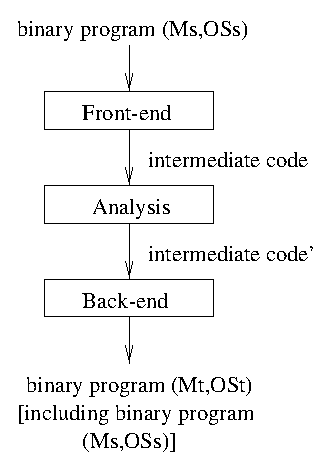
\includegraphics{figures/static.eps}}
\centerfigend{fig-static}{Structure of a static binary translator for
	source machine $M_s$, target machine $M_t$, source operating system
    $OS_s$ and target operating system $OS_t$.}
 
The fallback mechanism used by static binary translators is a runtime
environment that completely supports the source platform, and
hence includes an interpreter for source machine instructions, and support
for translation and mapping of operating system calls into the new
platform.  The development of a runtime environment is a significant
overhead; especially the mapping of operating system calls.  There is
little performance data reported in the literature regarding the amount of
time spent by binary translated applications in the interpreter mode.
Code ported from a proprietary CISC to RISC machine at Tandem, where the
operating system was binary translated to the new machine, reports an
average figure of 1\% of the time being spent on interpretation~\cite{Andr92}.
Informal talks with people who have developed such translators state that
the interpretation mode is seldom used if you have sufficient coverage 
of the patterns generated by compilers commonly used in that platform. 
Existing static translators have dealt mainly with procedural code, 
rather than object-oriented code, which poses new limitations to static
translation due to their dynamic nature of code dispatching through 
vtables.  
 
 
\subsection{Dynamic binary translator}
A dynamic binary translator performs the translation of the code while 
the program is being executed by the translator; that is, the input 
binary program is dynamically analyzed and translated into the target 
machine code during runtime.
Dynamic translation techniques overcome some of the shortages of static
translation, for example, determining the targets of indirect jumps.
Dynamic translation is able to support most practical cases of 
self-modifying code; code normally not supported in static translations.
Given that all the processing of a dynamic translator is done ``on the
fly'', the types of optimizations and analyzes have to be carefully
considered and optimized so that the minimum amount of time is spent
during runtime.
 
The structure of a dynamic binary translator is depicted in
Figure~\ref{fig-dynamic}\footnote{
Figure~\ref{fig-dynamic} by the SELF team at Sun Microsystems Labs.}.  
The binary program is fed into the front end which generates an 
intermediate representation for a block of code.  This representation 
is then compiled or emulated by the translator to generate
(unoptimized) machine code for the target machine.  If at any time the
translator determines that a new region of the program needs to be decoded,
the front end is dynamically invoked to parse that region and provide the
intermediate representation.  When generating machine code, counters are
kept on the number of times blocks of code are executed; once a threshold is
reached, machine code is regenerated to produce better machine code---this
process can be repeated several times, hence producing better code on a
demand-driven basis.  It is important to note that the translation is done
in a lazy fashion; that is, code is only translated when its path is reached.
In this way, fragments of the program that are not executed during runtime,
are not translated either.  Self-modifying code is handled by
invalidating the existing intermediate representation and re-parsing
the binary code with the changed bytes.
 
\centerfigbegin
\resizebox{!}{6cm}
{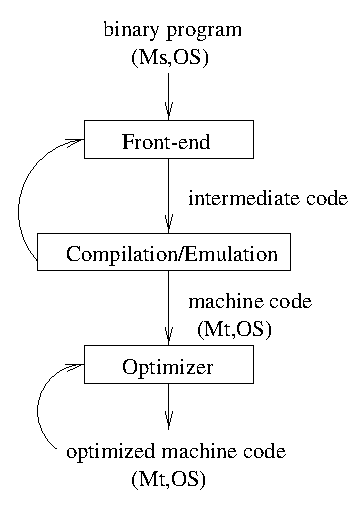
\includegraphics{figures/dynamic.eps}}
\centerfigend{fig-dynamic}{Structure of a dynamic binary translator for
    a source machine Ms, a target machine Mt and a multi-platform
    operating system OS.}
 
Dynamic compilers can perform runtime optimizations of the code based
on the execution profile of the program, hence several optimizations,
such as dynamically-dispatched calls and procedure inlining, can only be
possibly done on a dynamic compiler rather than using static techniques.
The performance penalty of code generated by such a translator is estimated
between 0.9X to 2.4X times that of code generated by a native optimizer
C++ compiler (these figures are based on code generated by the SELF-93 dynamic
compiler~\cite{Holz95}).
 
An interesting point to note is that a dynamic binary translator for
a multi-platform operating system does not require the development of
a runtime environment to support the mapping of old operating system
calls, as all translations are done ``on the fly''.  Using static techniques
in this case will still require a runtime environment to cater for the
interpretation of old machine instructions--dynamic techniques alleviate
the need for this fallback mechanism, but compromise the speed of 
execution of the program at the expense of less analysis and code
quality.
 




	
\chapter{Previous Work}
\label{ch-prevwork}

{\small
\begin{flushright}
Documentation: Cristina [c.1996, 2001]
\end{flushright} 
}

Binary translation is a relatively new field of research, were the
techniques are derived from the compilation, emulation and decompilation areas. 
Nevertheless, the techniques are ad hoc in nature and little has been 
published about them (mainly driven by commercial interests of the parties
involved).  

In this chapter we describe the related work, which we have classified
into two main groups: works related to binary translation and interpreters 
(or emulators), and works related to binary-code manipulation tools that 
may aid in the process.


\section{Binary translators and interpreters} 
Binary translation techniques were developed from emulation
techniques at research labs in the late 1980s.  Projects
like the HP3000 emulation on HP Precision Architecture
computers~\cite{Berg87} and MIMIC, an IBM System/370 simulator on an
IBM RT (RISC) PC~\cite{May87} were the catalist for these techniques.
One of the goals of the HP project was to run existing MPE V binaries
on the new MPE XL operating system.  For this purpose, a compatibility
mode environment was provided, which was composed of two systems:
a HP 3000 emulator and a HP 3000 object code translator.  The emulator
duplicated the behavior of the legacy hardware, and the translator
provided efficient translated code which relied on the emulator
when indirect transfers of control where met.

Tandem developed an object code translator for TNS CISC binaries
to TNS/R (RISC) in order to provide a migration path for existing
vendor and user software~\cite{Andr92}.  This approach allowed
them to market their new RISC machines years earlier than if no
migration path was available.  Part of the rationale for the
project was also the fact that no reprogramming was involved and
that the techniques would provide faster code than emulation
techniques.  Less than 1\% of the time was spent on emulation.

Digital developed two translators, VEST and mx, to provide a migration
path from their OpenVMS VAX and Ultrix MIPS systems to their new
Alpha machine~\cite{Site92,Site93}.  Interestingly enough, they
decided to do careful static translation once instead of on-the-fly
dynamic translation at each execution time for performance issues.
In both their translators, the old and new environments were, by
design, quite similar, plus both provided similar operating system
services.  Some of the goals were to take full advantage of the
performance capabilities of the Alpha and avoiding the problem of
not having all the tools available to port a program to a new architecture
(because they are still not available on the new hardware).
This was seen as an interim solution, while the user's environment was
made available on the new machine and then code could be recompiled/rebuilt.

Up to 1992 all translators were made available by hardware                   
manufacturers to provide a migration path from their legacy
hardware platform (normally a CISC) to their new platform
(normally a RISC).

Back in 1994, AT\&T Bell Laboratories provided services to migrate
software in object code form from one platform to another through
the FlashPort binary translator~\cite{Att94}.
Translations of PDP 11, 680x0 and IBM 360 code was made to
platforms like MIPS, RS/6000, PowerPC and SPARC.  Translation
time was based on the type of application, with some large
applications being translated in 1 month, whereas others in
6 months; which means that manual changes were done to assure
consistency of the translation, plus to provide compatibility
libraries to cater for the differences in operating systems and
services.
The FlashPort technology was initially developed by Bell Laboratories
researchers and was commercialized through the 1991-formed Echo
Logic company.  The first production release of the technology
was provided to Apple Computers in 1993 to translate Macintosh
binaries to the then forthcoming PowerPC-based Macintosh computers.

In an attempt to make Alpha machines more appealing to existing
Unix users, Digital released FreePort Express, a SunOS SPARC
static binary translator to Digital Unix Alpha~\cite{Dec95};
particularly at a time when Sun was migrating customers to
their new Solaris OS and discontinuing support for SunOS.
The tool was advertised as a way of migrating to the Alpha even
when source code and compiler tools from the source machine
were not available; then do a native port at your own leisure.
Since the translated programs and libraries provided support for
Xview, OpenLook, Motif and other X11-based applications, this
migration path was suitable for users who did not want to be
trained in the use of new tools.

To improve Alpha's usability as a desktop alternative to Intel
PCs, Digital developed FX!32, an WindowsNT x86 to WindowsNT Alpha
translator~\cite{Thom96,Hook97}.  Emulation was used as it provided
a quick way to provide support for changes in WindowsNT.  However,
binary translation on the background was also used in order to
save the translations to a file and, over time, incrementally
build the new Alpha binary.  This hybrid translator uses profiling
information in order to optimize the code the next time it
is run.

The TIBBIT project looks at real-time applications that are to be
binary translated between processors of different speeds~\cite{Cogs95,Cogs95b}.
The translated software needs to retain the implicit time-dependency
of the old software in order to function correctly.

\begin{table*}[hbtp]
{\footnotesize
\begin{tabular}{|p{1.5cm}|p{1.3cm}|p{0.7cm}|p{5cm}|p{2cm}|p{2cm}|} \hline
Name & Affiliation & Ref & Purpose & Source Platform & Target Platform \\ \hline
Bergh et al (1987) & HP & \cite{Berg87} &
	Software emulation and object code translation. &
	(HP3000, MPE V) &
	(HP Precision Architecture, MPE XL) \\
Mimic (1987) & IBM & \cite{May87} &
	Software emulator with a 1:4 code expansion factor per 
	old machine instruction. &
	IBM System/370 &
	IBM RT PC \\
Johnson (1990) & Stardent & \cite{John90} &
	Postloading optimizations. &
	RISC &
	RISC \\
Bedichek et al (1990) & U.Wash & \cite{Bedi90} &
	Efficient architecture simulation and debugging. &
	Motorola 88000 &
	Motorola 88000 \\
Accelerator (1992) & Tandem & \cite{Andr92}        &
	Static binary translation for CISC to RISC migration.  
	Uses a fallback interpreter.    &
	TNS CISC        &
	TNS/R   \\
VEST, mx (1993) & Digital & \cite{Site93} &
	Static binary translation from Digital's VAX and MIPS machines
	to the 64-bit Alpha.  Uses a fallback interpreter. &
	(VAX, OpenVMS), (MIPS, Ultrix) &
	(Alpha, OpenVMS), (Alpha, OSF/1) \\
Wabi (1994) & Sun & \cite{Sun94} &
	Pretranslated Windows API to Unix API calls.  Dynamic execution of 
	programs. &
	(x86, Windows 3.x) &
	(SPARC, Solaris) \\
Flashport (1994) & AT\&T & \cite{Att94} &
	Binary translation across a variety of source and target platforms.
	Requires human intervention. & 
	680x0 Mac, IBM System/360, 370, 380 &
	PowerMac, IBM RS/6000, SPARC, HP, MIPS, Pentium \\
Shade (1994) & Sun & \cite{Cmel94} &
	Efficient instruction-set simulation and trace generation
	capability.  Dynamic compilation of code. &
	SPARC V8, V9 &
	SPARC V9, V8 \\
MAE (1994) & Apple & \cite{Apple94} &
	Macintosh environment in an XWindow, Unix RISC-based workstation. &
	680x0 &
	RISC-based Unix \\
Wahbe et al (1994) & CMU & \cite{Wahb94} &
	Adaptable binaries.  Binary transformations.&
	(MIPS, Ultrix4.2) &
	(MIPS, Ultrix4.2) \\
Chia (1995) & Purdue & \cite{Chia95} &
	Software emulation within the same platform, with a 1:100 code
	expansion factor per old machine instruction. &
	(SPARC, Solaris) &
	(SPARC, Solaris) \\
TIBBIT (1995) & CMU, UO & \cite{Cogs95,Cogs95b} &
	Binary translation of time-sensitive applications.&
	Motorola 68000 &
	(IBM RS/6000, AIX 3.2) \\
Then (1995) & Purdue & \cite{Then95} &
	Optimization of code within the same platform.&
	(SPARC, Solaris) &
	(SPARC, Solaris) \\
Freeport Express (1995) & Digital & \cite{Dec95} &
	Static binary translation and fallback interpreter.  Translates
	user mode programs. 32-bit to 64-bit translation. &
	(SPARC, SunOS4.1.x) &
	(Alpha, OSF/1) \\
FX!32 (1996) & Digital & \cite{Thom96,Hook97} &
	Hybrid emulator/binary translator of popular x86 32-bit applications 
	to Alpha.   &
	(x86, WindowsNT) &
	(Alpha, WindowsNT) \\
\hline
\end{tabular}
\caption{\label{tab-bintrans} {Summary of Binary Translators and
	Interpreters in Cronological Order.}}}
\end{table*}

We summarize the features of a variety of binary translators and
interpreters in Table~\ref{tab-bintrans}.  The column {\em Purpose\/} 
describes the general use of the tool, columns {\em Source Platform\/}
and {\em Target Platform\/} describe the nature of the translation supported
by the tool (i.e. multi-platform or within the one platform), 
column {\em Name\/} refers to the name of the software; if unnamed, then
it refers to the people that worked on it, and column {\it Affiliation}
refers to the affiliation of the authors of the software at the time
of development. 


\subsection{List of recent translators}
There has been a lot of work in the last few years (1998-2000) 
on dynamic techniques for doing binary manipulation of one sort of 
another.  The following is a list of projects and literature available: 

\begin{itemize}
\item HP Aries~\cite{Zhen00}: 
Aries is a hybrid interpreter/dynamic translator which
allows PA/RISC HP-UX binaries to run in an IA-64 HP-UX
environment transparently, without user intervention.

\item HP Labs Dynamo~\cite{Bala00}: 
Dynamo is a dynamic reoptimizer of PA-RISC binaries which
produces PA-RISC code.  It works well for some programs 
and not for others. 

\item IBM TJ Watson Research Center's DAISY~\cite{Ebci96} and 
BOA~\cite{Gsch00}: 
The DAISY and BOA projects have looked at dynamic binary translation 
from conventional architectures such as the PowerPC to VLIW or other
novel architectures.  Their work addresses precise exceptions, 
self-modifying code, and reordering of memory references; all of 
these from an architectural point of view. 

\item Transmeta's Crusoe~\cite{Gepp00}: 
The Crusoe chip is a VLIW chip which includes code morphing to 
dynamically binary translate from x86 to the VLIW instruction set. 
Some x86 instructions are supported by the hardware itself. 

\item Compaq's Wiggins/Redstone~\cite{Reev00}: 
Wiggins/Redstone was a dynamic reoptimizer of Alpha binary code. 
It was built based on Digital's DCPI infrastructure.  

\end{itemize}



\section{Binary-code manipulation tools}

\begin{table*}[hbtp]
{\small
\begin{tabular}{|p{2.0cm}|p{0.7cm}|p{7.8cm}|p{3.0cm}|} \hline
Name & Ref & Purpose & Platform \\ \hline
Silberman et al (1993) & \cite{Silb93} &
	Framework for supporting heterogeneous instruction set architectures. &
	CISC, RISC, VLIW \\
QPT (1994) & \cite{Laru94} &
	Rewrite executable files to measure program behavior. &
	MIPS, SPARC \\
Shade (1994) & \cite{Cmel94} &
	Execution profiling of application binaries. &
	SPARC V8, V9 \\
ATOM (1994) & \cite{Dec94,Eust95} &
	Sytem for building customized program analysis tools. &
	(DecStation, Ultrix), (Alpha, OSF/1) \\
NJMC (1994) & \cite{Rams95,Rams94,Rams97} & 
	Machine-independent encoding and decoding of machine instructions
	via the SLED language. &
	MIPS, SPARC, x86, PowerPC, Alpha \\
EEL (1995) & \cite{Laru95} &
	Library for editing binaries. &
	MIPS, SPARC \\
\hline
\end{tabular}
\caption{\label{tab-bintools} {Summary of Binary-code Manipulation  
	Tools in Cronological Order.}}
}
\end{table*}

Table~\ref{tab-bintools} summarizes the available tools for handling
machine binary code.  The column \emph{Name} lists the name of the
tool (or its author if no name was given to the tool), column 
\emph{Ref} lists the references in the literature to this tool,
column \emph{Purpose} describes the purpose of the tool, and column 
\emph{Platform} lists the platform(s) supported by these tools. 

ATOM is a tool-building system that provides a flexible and efficient
interface for the instrumentation of code and has been used for the
construction of an instruction profiler, cache simulator and compiler
auditing tool~\cite{Eust95}.  The user needs to write an instrumentation
file in terms of ATOM's abstractions (procedures and basic blocks),
and an analysis file (using a high-level language such as C) with the 
routines that are to be included for instrumentation purposes.  
The performance of the generated tools compare favourably with 
hand-crafted implementations of same the tools. 

Shade is an instruction-set simulator which optionally allows users to 
profile code that traces the execution of an application at runtime.  
Trace information on instruction addresses, instruction text, decoded
opcode values, and more can be collected by Shade~\cite{Cmel94}.
This tool works only on SPARC machines.

Both NJMC (New Jersey Machine-Code) toolkit~\cite{Rams95,Rams97} and EEL
(Executable Editing Library)~\cite{Laru95} provide support for
manipulating machine instructions.  The NJMC toolkit supports the 
encoding and decoding of machine instructions for a variety of 
RISC and CISC machines, by means of SLED specifications.  
The SLED language allows for the description of the syntax of machine 
instructions in a specification that resembles instruction descriptions 
found in architecture manuals.
The toolkit has successfully been used in a retargetable 
linker~\cite{Fern95} and a retargetable debugger~\cite{Rams92}.  
The EEL library was built based on the NJMC machine specifications, 
and introduced control flow support based on techniques developed in 
the QPT~\cite{Laru94} profiler.  EEL also introduced limited
support for describing the semantics of machine instructions.
The tool is not fully portable to non RISC environments.




	
\chapter{The UQBT Framework}
\label{ch-uqbt-framework}

{\small
\begin{flushright}
Design: Cristina, Norman; Documentation: Cristina [c.98, May 00, Nov 01]
\end{flushright} 
}

The University of Queensland Binary Translator (UQBT) 
framework, is designed to support experimentation in static
binary translation.
UQBT strives to adapt easily to changes in both source and
target machines at low cost, including translations to
register-based and stack-based machines.
Support for multiple architectures is provided by means
of specification of properties of machines, as well as 
conventions used by operating systems.  
This chapter describes the overall architectural organization
of \uqbt\ (Section~\ref{sec-arch}) and its components from the point of view 
of instruction translation (Section~\ref{sec-framework}).  Note that
these two sections are necessarily overlapping; the former
section reflects more of the design and the latter section
reflects more of the implementation of the system.  
The chapter concludes with a small section on the state of the
UQBT framework at the end of 2001. 


\section{The Proposed 1997 Architecture of a Retargetable Binary Translator}
\label{sec-arch}

Like a compiler and a decompiler, a binary translator can logically
be divided into three phases: front end, analysis and transformation,
and back end.  For a given source machine M$_s$ and destination machine M$_d$,
the front end decodes machine M$_s$'s binary file and stores the 
information in a machine-independent intermediate form based on RTLs.
The analysis phase maps machine M$_s$'s locations onto machine M$_d$'s 
locations and transforms the RTLs so that they can be readily translated into 
native code for machine M$_d$.  The back end translates the intermediate 
form and writes a binary file for machine M$_d$.  It may also optimize 
instructions.

From a retargetability point of view, it is more helpful to think of 
a functional division into components instead of a sequential division 
into phases.  Such components may be used in more than one phase.
Some components will be machine-independent; others may be generated 
from machine descriptions.  In Figure~\ref{fig-architecture}, we identify 
components by putting them in boxes.

% original file created in Visio, printed to a file using Adobe's Default
% Postscript Printer driver (option EPS), and crop with ghostview (gsview 
% on the PC version 2.5) using File->PStoEPS option.
\centerfigbegin
\resizebox{!}{10cm}
{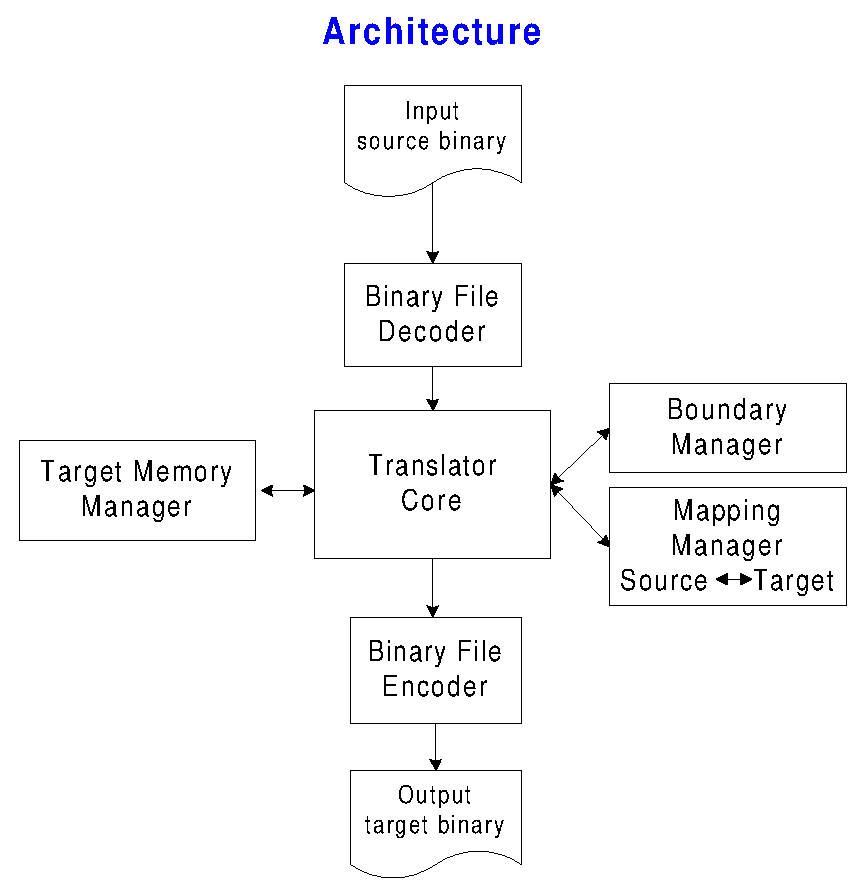
\includegraphics{figures/uqbt_architecture.eps}}
\centerfigend{fig-architecture}{Architecture for a Retargetable Binary
	Translator.  Components are Represented in Boxes.}

Implementation of components draws on techniques developed for
dcc, an 80286 decompiler~\cite{Cifu95}, for specifying
representations of machine instructions~\cite{Rams97},
and for the U.S. National Compiler Infrastructure project.


\subsection{Components}

M$_s$ \emph{binary file reader} exports an abstraction
representing the contents of the executable binary on the original
machine.  This module promotes retargetability by hiding
information about the source machine that one might otherwise be
tempted to exploit.  The capabilities exported include:
%\enumerateAlpha
\begin{enumerate}
\item The initial state of the M$_s$ processor that would apply when about
     to run this binary on a native M$_s$ processor, including at minimum
     the value of the program counter,
\item A list of potential entry points for procedures, possibly empty
     (N.B. the initial program counter is always available as an entry
     point), 
\item The ability to fetch the program's code and data, by the address
     those contents would occupy in a running M$_s$ executable, and 
\item The ability to identify calls to dynamically linked procedures, and
     to provide access to the code and data associated with those
     procedures.
\end{enumerate}
%\enumerateNumber
This module may therefore include much of the functionality of a dynamic
linker/loader.

One of the crucial decisions made by a translator is which locations
on machine M$_d$ hold what data from machine M$_s$.  We will encapsulate these
decisions in a \emph{mapping manager}, which will map locations in code
space, locations in data space, and locations referring to registers
or other processor state.  Most mappings will be determined
automatically at translation time, but some mappings may be specified
by hand for each pair of platforms, e.g., what registers of machine M$_d$
should be used to represent the contents of registers of machine M$_s$.

The mapping manager will rely on the M$_d$ \emph{memory manager} to allocate 
locations in the destination machine's storage space, e.g., to store 
translated code.

Because it is impossible to identify and translate all code, a running
image on machine M$_d$ will in general have a mix of translated and
untranslated code.  The \emph{boundary manager} will track the boundary
between translated and untranslated code and handle flow of control
across the boundary.  For example, a branch from translated to
untranslated code might go to an interpreter or to a dynamic
translator.  If the untranslated code is subsequently translated, the
boundary moves, and the boundary manager might backpatch the branch.

The \emph{core translator} will translate groups of machine instructions.
A group may be as small as a basic block or as large as an entire 
program, and different translation strategies (e.g., full static, 
partial static, dynamic) may use different group sizes.

The core translator coordinates the action of all the other
components and performs the main translation analyses.  It will 
translate a group of M$_s$ instructions as follows:
%\enumerateAlpha
\begin{enumerate}
\item Ask the memory manager for a location in M$_d$ to hold the translated
     code, and inform the mapping manager of the new mapping, 
\item Translate M$_s$ instructions to M$_d$ instructions
	  \begin{itemize}
      \item using information from the mapping manager to translate
         access to machine M$_s$'s data, 
      \item using information from the boundary manager to translate flow
	  \end{itemize}
	 of control outside the current group, and
\item Inform the boundary manager of the translation of the current group.
     The boundary manager may choose to backpatch branches into the
     current group.
\end{enumerate}
%\enumerateNumber
Depending on the granularity and timing of translation, these steps may
be repeated on other units until some termination condition is met.
If the granularity of translation is sufficiently large, the second step
may involve translating into an intermediate form and doing some global
analysis and optimization.

Finally, the M$_d$ \emph{binary file writer} will export an abstraction
representing the ability to create an executable binary on machine M$_d$.
It will export the abilities to:
%\enumerateAlpha
\begin{enumerate}
\item Specify the contents of the M$_d$ address space at the start of
     execution,
\item Establish the state of the M$_d$ processor at the start of execution,
\item Write an executable binary file in the M$_d$ native format, and
\item Possible support for dynamic linking, e.g. of translated or native
     libraries.
\end{enumerate}
%\enumerateNumber
In a dynamic translator, this component would simply write into a
running process image (and possible flush the I-cache).


\subsection{Core Translation based on RTLs}

The translation itself will be performed using register transfer lists
(RTLs).  An RTL is a collection of simultaneous effects.  Each effect
has the form `location := expression', and the expression is always
evaluated without side effects, so all state change is explicit.  
RTL expressions are represented as trees, the leaves of which refer to
constants or to the values contained in locations.  Note that although
the tree leaves refer to locations, the values themselves are not
necessarily calculated, only the location is referenced.
The internal nodes of the trees are `RTL operators'.  
For illustrative purposes, the following is an ASCII representation of an 
RTL representing the effect of the SPARC \texttt{andcc} instruction:
\begin{smallverbatim}
 $r[rd] <--      and (*$r[rs1], if i = 0 then *$r[rs2] else simm13! fi);
 icc.N  <-- bit (and (*$r[rs1], if i = 0 then *$r[rs2] else simm13! fi) < 0);
 icc.Z  <-- bit (and (*$r[rs1], if i = 0 then *$r[rs2] else simm13! fi) = 0);
 icc.V  <-- 0;
 icc.C  <-- 0
\end{smallverbatim}
This RTL does a bitwise AND of the contents of register rs1, either
with the contents of register rs2 or with a signed immediate value (simm13).
This result is stored in register rd, and it is also used to set two
of the four condition codes.  The other two condition codes are set to 
zero by the instruction.

RTLs are obviously complex and detailed.  Machine descriptions
themselves will be written at a higher level of abstraction and
compiled into RTLs.  Run-time representations of RTLs will be
`collapsed' either by analyzing these higher-level representations or
by using the `superoperator' technique~\cite{Proe95}.  
For example, we might define a superoperator LOGICAL such that LOGICAL(X)
stood for
\begin{smallverbatim}
 $r[rd] <--      X;
 icc.N  <-- bit ((X) < 0);
 icc.Z  <-- bit ((X) = 0);
 icc.V  <-- 0;
 icc.C  <-- 0
\end{smallverbatim}
Such a superoperator could be derived from the SPARC description. 

An `RTL language' is defined by a collection of locations and
operators.  For binary translation, a suitable RTL language can be
defined by taking the union of locations on machines M$_s$ and M$_d$ and the
union of the operators used in the descriptions of machine M$_s$ and M$_d$.
The `machine X invariant' defines a sub-language of RTLs called the
X-RTLs; an RTL is an X-RTL if and only if it can be represented as a
single instruction on machine X.

% original figure in Visio, exported as eps (without including TIFF
% preview or background rectangle).
\centerfigbegin
\resizebox{!}{12cm}
{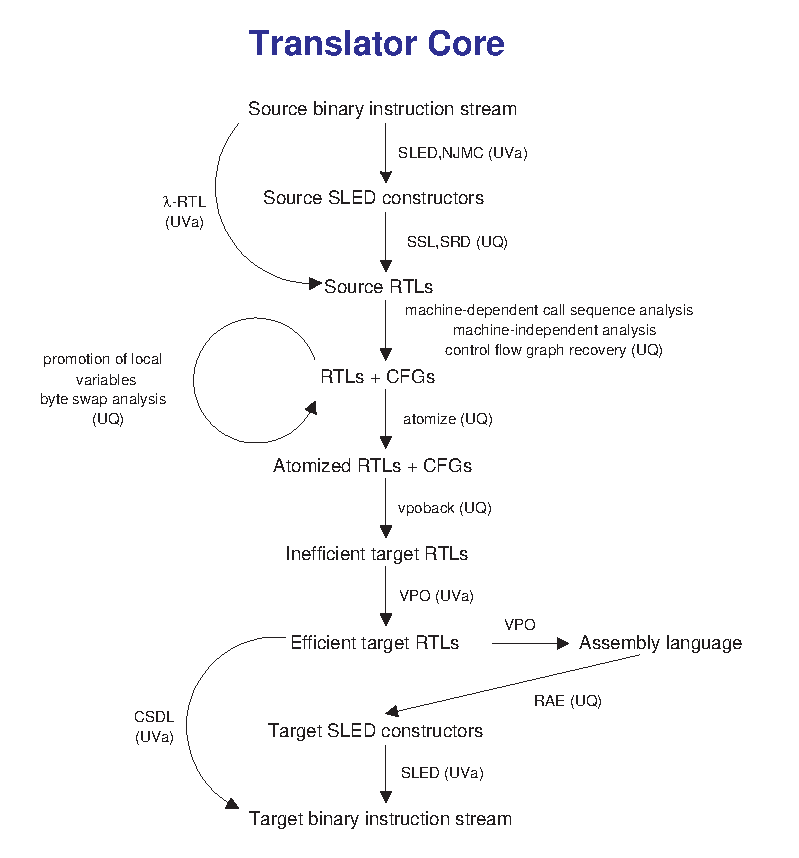
\includegraphics{figures/uqbt_dataflow.eps}}
\centerfigend{fig-dataflow}{Flow of Data through the System}

As shown in Figure~\ref{fig-dataflow}, the main steps in the translation are:
\begin{enumerate}
\item Decode the binary stream into M$_s$-RTLs.  This step will be
     automated by specifying syntax and semantics of M$_s$ instructions.

\item Build a control flow graph (CFG) for each procedure.  Analysis
     will be needed to find code associated with a procedure.

\item With the help of the mapping manager, map the machine M$_s$ locations
     in the RTLs to machine M$_d$ locations or to temporaries.

\item `Atomize' the RTLs to expose all RTL operators at top level, and
     find suitable replacements for machine M$_s$ operators that are not
     available on machine M$_d$.  For example, big-endian memory access
     might be replaced with explicit byte swapping.

\item Reassemble the RTLs to satisfy the machine M$_d$ invariant, making
	them M$_d$-RTLs (i.e. M$_d$-RTLs have a 1:1 mapping with M$_d$ 
	assembly instructions).

\item Optimize the M$_d$-RTLs using VPO~\cite{Beni88} or any other RTL 
	optimizer.

\item Encode the M$_d$-RTLs into binary code for machine M$_d$.  Also automated.
\end{enumerate}

The most challenging steps are steps (4) and (5).  In the initial
stages, these will be implemented by hand; we hope to develop automated
techniques afterwards.  The other steps can be automated based on
machine descriptions or a mapping specification.

Future analyses, intended to improve translated code, might be
implemented after steps (2), (3), or (4).  Such analyses might make it
possible to avoid byte swapping, to use machine M$_d$ calling conventions,
to put machine M$_s$ stack variables in machine M$_d$ registers, etc.
Analyses may vary depending on the granularity of translation.


\section{The 1999 UQBT Framework}
\label{sec-framework}

In order to support resourceability and retargetability, 
machine descriptions of machine properties are needed, 
as well as descriptions of conventions and formats used by 
the operating system.  We have identified 6 different specification 
languages and/or APIs to support the UQBT framework, 4 of these are 
currently in use in our framework. 

The framework described in this section dates from 1998, 
Section~\ref{sec-2001framework} describes the 2001 framework. 
References in this section are to papers and chapters within 
this book that explain in more detail a particular concept. 


\subsubsection*{Machine specifications and APIs} 
Properties of a machine are represented in terms of the machine 
instructions (i.e. the mnemonics), the semantics of such instructions, 
the identification of the instructions that transfer flow of control, 
and, if needed, delayed transfers of control information.  
These 4 types of information are represented by the following 
languages: 

  \begin{itemize}
  \item SLED (Specification Language for Encoding and Decoding), 
	which supports descriptions of the syntax of machine 
	instructions~\cite{Rams97}.  [Chapter~\ref{ch-decoding}];

  \item SSL (Semantic Specification Language), which supports 
	descriptions of the semantics of machine 
	instructions~\cite{Cifu98c}.  [Chapter~\ref{ch-ssl}]; 

  \item CTL (Control Transfer Language), which supports the 
	identification of instructions that perform control 
	transfers of control (conditional jumps, jumps, calls or 
	returns). This language was implemented as a loose API in the
	end, as we decided not to specify other transfer of control 
	information in the end.  

  \item DCTL (Delayed Control Transfer Language), which supports 
	the description of simple transformations needed in 
	order to remove dependencies on delayed instructions (in 
	machines that support such concept).  

    Support for DCTL is not in place at present.  Initially, we used 
    a program-transformation and partial-evaluation technique to derive 
    the transformations on instructions that support delayed transfers of 
    control~\cite{Cifu98i}.  [Chapter~\ref{ch-delay}].
    The code is voluminous and we believe that code to support such 
    transformations could be automated from a short specification 
    of the required transformations.  This step would clearly increase 
    the resourceability of the framework.  However, we note that not 
    too many machines currently support the delayed-slot transfer of 
    control, only SPARC, PA-RISC and MIPS do at present time.

  \end{itemize}


\subsubsection*{OS specifications/APIs} 
Conventions and formats used by a multiplatform operating system come 
in the form of calling conventions, including where parameters are passed 
(i.e. stack or registers), and the format of the binary-file that the 
OS supports.  
These 2 pieces of information are represented by the following 
languages/APIs: 

  \begin{itemize}
  \item PAL (Procedural Abstraction Language), which supports 
	the description of calling conventions, parameter passing conventions, 
	and local variables conventions~\cite{Cifu99g}. [Chapter~\ref{ch-call}];  
	and 

  \item BFF (Binary File Format), which supports the description 
	of the internal format of a binary-file, such as the 
	Elf format on Solaris and Linux systems~\cite{Cifu97f}. 
	[Chapter~\ref{ch-bff}].  
  \end{itemize} 

We currently support the PAL language and have worked on 
an initial prototype of the BFF language, which is incomplete 
at present time but proves the feasibility of specifying 
binary-file formats and automatically generating code to 
support the decoding of such files.  In our experience, it 
was easier to have a set API for dealing with differences in 
binary-file formats than to specify the existing ones.   

\psfigbegin{figures/uqbtImplementation.eps}{10cm}
\psfigend{fig-uqbt}{Framework for a Resourceable Binary Translator.}

Figure~\ref{fig-uqbt} illustrates the components of the 
translation process in the form of boxes.  Specifications for different
machines are illustrated with the document shape.
Greyed-out shapes mean that they are not currently supported 
by UQBT and therefore an implementation for a particular format 
or analysis has been done instead.  Arrows represent conceptual 
flow of control in the translation process.  


\subsection{The Decoding Phase}
The binary-file decoder, instruction decoder 
and semantic mapper translate raw machine instructions into  
M$_s$-RTLs for a given source machine M$_s$.  
As previously mentioned, we consider M$_s$-RTLs machine dependent, as
they represent how the source machine performs a given instruction, 
including delayed-slot semantics for example.  

In static translators, the amount of decoding from this phase 
is limited by indirect transfers of control (i.e. statically,  
it is not always possible to determine the target of an 
indexed jump or an indirect call).  
UQBT includes a slicing-based technique to determine the target
address(es) of indirect transfers of control~\cite{Cifu99c}. 
This technique allows us to decode a larger percentage of the
code than otherwise possible, and is reusable across different 
platforms.  


\subsection{The Analysis Phase} 
The translation of M$_S$-RTLs up to \hrtl\ is 
the most challenging stage of the translator.  As seen in 
Figure~\ref{fig-uqbt}, this translation requires information 
about control transfer instructions, delayed control transfers 
(if any), parameter and calling conventions, and locals and 
stack frame conventions.  
CTL specifications allow us to translate low-level register 
transfers into higher level instructions such as calls and 
returns.  
For example, a CTL specification for SPARC states that a 
jump and link instruction with destination register \texttt{\%o7} 
is a call instruction.  This semantics is not necessarily 
obvious from the SSL description of a jump and link instruction. 
Further, the same instruction using destination register 
\texttt{\%g0} is equivalent to an unconditional jump; this 
too is specified in CTL.  

DCTL specifications will allow us to remove delayed-slot 
instructions in a more machine-independent way.  
At present, as previously mentioned, we implement a program
transformation and partial evaluation technique. 

PAL specifications allow us to recover some of the high-level nature 
of the code, by recovering actual parameters and return 
values for functions, and removing the M$_S$-RTL-specific 
instructions that form part of procedure prologues and 
epilogues, as these are represented in different ways in 
different machines.  The analysis is based on live and 
used parameter and return locations; such locations being
specified in a PAL specification, as well as abstraction to 
an abstract frame pointer (\texttt{\%afp}).  
For example, a PAL specification for the Pentium would specify
that parameters can be passed on the stack and that return 
values go into certain registers (\texttt{\%eax} and top of 
the floating point stack). 
A more detailed description of the analysis is available 
in~\cite{Cifu99g} and Chapter~\ref{ch-call}. 
 
\centerfigbegin
\begin{fnverbatim}
r[tmp] = %sp
r[tmp2] := -120
%pwp = %cwp
%cwp = %cwp + 64
%cwp = (%cwp-1) % NWINDOWS
%sp = r[tmp] + r[tmp2]
r[9] = 69 << 10            v1 = 70656
r[8] = r[9] | 720          v0 = v1 | 720
r[15] = %pc
%pc = %npc
%npc = 0x21780             Call printf (v0, v1)
r[9] = r[30] + -20         v1 = %afp + 100
r[10] = 69 << 10           v2 = 70656
r[8] = r[10] | 736         v0 = v2 | 736
r[15] = %pc
%pc = %npc
%npc = 0x2178c             Call scanf (v0, v1, v2)
r[8] := m[r[30] - 20]      v0 = m[%afp + 100]
r[15] = %pc
%pc = %npc
%npc = 0x10a9c             v0 = Call fib (v0)
m[r[30] - 24] = r[8]       m[%afp + 96] = v0
\end{fnverbatim}
\centerfigend{fig-palEg}{Example of the result of the use of PAL
        specifications to translate SPARC-RTL code (left-hand side)
        to \hrtl\ (right-hand side) in a fibonacci program.}

Figure~\ref{fig-palEg} illustrates 
a snippet of SPARC-RTLs for the \texttt{main} of a fibonacci 
program, and the resultant \hrtl\ code.  As can be seen, 
the RTLs for the procedure prologue were removed (and relevant information
used in the translation), the actual parameters to library functions 
\texttt{printf} and \texttt{scanf} are listed, actual parameters 
were moved to variable locations, local variables are in terms of 
an abstract frame pointer called \texttt{\%afp}, and the return 
value for the call to \texttt{fib} has been determined.   
The example also shows that the call to \texttt{fib} has the
right number of parameters (i.e. one), and that the calls to
the variable argument routines \texttt{printf} and \texttt{scanf} 
each take one extra parameter than expected.  These parameters were passed 
as they were live and were valid parameter locations at the 
call site.  However, when the code is executed, these parameters
will not be used as the library routines would not be expecting
these parameters for processing (i.e. the format string 
in both these routines specifies the number of parameters
required to be processed), therefore producing the right
result at runtime.  

Lifting the level of representation of the code to \hrtl\ 
allows for experimentation with different types  
of binary translation-specific optimizations, such as removing 
some of the byte swaps at loads and stores when machines have  
different endianness, or promoting local variables to registers. 
This is future work. 


\subsection{The Encoding Phase} 
\label{sec-encoding}

\centerfigbegin
\begin{fnverbatim}
void main() {
int v0;
int v1;
int v2;
char _locals[120];

        v1=70656;
        v0=(v1)|(720);
        printf(v0,v1);
        v1=(_locals)+(100);
        v2=70656;
        v0=(v2)|(736);
        scanf(v0,v1,v2);
        v0=*((int*)((_locals)+(100)));
        v0=fib(v0);
        *((int*)((_locals)+(96)))=v0;
\end{fnverbatim}
\centerfigend{fig-cEg}{Example generated low-level C code for the partial
        fibonacci example of Figure~\ref{fig-palEg}.}

The last step in this phase is the translation down to the 
target machine's intermediate representation; M$_T$-RTL in 
the case of register-based machines or \bcode\ in the case 
of stack-based machines.  
The translated code will always require an optimizer to improve 
its quality, therefore, the encoder phase would be equivalent 
to that of an optimizing compiler.  Because we interface 
to existing C optimizing compilers, we generate very low-level 
C code from this step.  Figure~\ref{fig-cEg} shows the 
generated low-level C code for the example in Figure~\ref{fig-palEg}. 
As can be seen, data addresses are not modified, therefore  
a call to \texttt{printf} or \texttt{scanf} takes the same 
memory address as that in the source binary.  

We have successfully interfaced to VPO~\cite{Beni88}, whose register 
transfer list interface is similar to our RTLs, and hence it is simple  
to translate to.  The new VPO interface is part of the Zephyr 
project~\cite{Vpo98}.  
Generating (low level) C allows us to experiment with different 
optimizers, and also is the interface to the stack based backends. 
For generation of code to the Java Virtual Machine (JVM), we 
have written a backend and a bytecode description that 
integrates with gcc. 

\centerfigbegin
\begin{fnverbatim}
                   ... (setup code)
v2=134517960;      ldc 124517960   ; put string in local 10
printf(v2);        istore 10
r24=(_afp)+(4);    aload_0         ; call _printf
v2=r24;            iload 10
v1=134517975;      invokevirtual Fibo/_printf (I) I
scanf(v1,v2);      istore 10
                   ldc 16          ; put afp+4 in local 12
                   lstore 9
                   iload 14
                   iload 9
                   iadd
                   istore 12
                   ldc 134517975   ; put string in local 10
                   istore 10
                   iload 12        ; put afp+4 in local 11
                   istore 11
                   aload_0         ; call _scanf
                   iload 10
                   iload 11
                   invokevirtual Fibo/_scanf(II)I
                   istore 10
\end{fnverbatim}
\centerfigend{fig-bcodeEg}{Example of generated bytecode after gcc
        optimizations (right-hand side) for low-level C code
        generated from Pentium fibonacci binary (left-hand side).}

The generation of bytecode via gcc provides us with all the
classical optimizations that are too computationally expensive to be
performed by a just-in-time compiler.  
We wrote a bytecode specification file for gcc which treats registers 
as locals and describes peephole optimizations.  
For each \hrtl\ instruction, $n$ bytecode instructions are 
generated, where $n$ is normally less than 5.  The generated
bytecode is similar to that generated by a Java compiler, 
given the high level of abstraction of the \hrtl\ code.  
Current work under development improves on the generated bytecode 
by using an intermediate language called \bcode, which allows 
for stack-based optimizations to be performed, therefore minimizing the 
amount of loads and stores from memory and using the stack 
for temporary values more. 
Figure~\ref{fig-bcodeEg} shows sample bytecode generated from our 
gcc bytecode backend.  Library calls are to wrapping routines 
which invoke the native Java library subsystems.  For variable
argument routines, we have $n$ different wrappers, where $n$ is
the number of parameters and typically $n$ is less than 10. 

For each translation, the generated code and data are 
placed into a variety of C and assembly files which can be 
compiled with gcc and gas on the target machine.  
For each function, a low-level C file is generated. 
For each data section, an assembly file is generated with the  
relevant bytes. 
A makefile is provided to pack the file into an appropriate 
binary for the target machine.

Static translators require the use of an interpreter/emulator to handle 
untranslated code that is discovered at run time.  
The interpreter uses the M$_S$-to-M$_T$ mapping to determine when 
it can return to translated code, and therefore this mapping is stored 
in the target binary.
Because the interpreter will use the original source text section, 
this section is also copied to the target binary.
The interpreter itself is designed to be linked dynamically.
We are currently building a resourceable interpreter/emulator which uses 
the same SLED and SSL specifications provided by the UQBT framework.
The interpreter simulates M$_s$-RTLs and uses PAL specifications 
to determine how to pass parameters to library routines.  
This work is not completed at present time and is under development.

Because of potential aliasing problems, not all of which can be solved by
static analysis, the data sections (generally .rodata and .data in 
Elf binary files) are copied ``as is'' to the target binary. 
They are made to retain the same Virtual Memory Address in the 
target binary as in the source binary. A link map file generated by 
the translator is used to achieve this. The target program calculates 
addresses exactly as the original source program did, and so the data 
is referenced correctly (although it may need to be referenced 
using different endianness). 
Because of differences in size of pages in various architectures 
(e.g. 4Kb on Pentium, verses typically 8Kb on SPARC), this mapping 
cannot always be achieved entirely by manipulation of addresses in the 
target binary file. A very small piece of code sometimes has to perform block 
moves (before the normal startup code) to achieve the correct addresses.

Translators to bytecode require extra environment support
to compliment the strengths of the JVM.  The lack of a generic memory
model on the JVM forces us to emulate the data and stack of a translated
program.  Library functions from the source architecture must also be
supplied to the translated program.  This is facilitated by a superclass
from which each translated program is inherited.  The superclass provides
simulated memory access in preloaded byte arrays and wrapper routines to 
library functions which invoke the native Java subsystems.


\section{The 2001 UQBT Framework}
\label{sec-2001framework}

\psfigbegin{figures/uqbtOverall2001.eps}{10cm}
\psfigend{fig-uqbt2001}{The 2001 UQBT Framework}

The final UQBT 2001 framework provides for several backends that 
were written for experimentation with different ways of generating 
machine code, by integrating at different levels of abstraction. 
Figure~\ref{fig-uqbt2001} shows this framework, we briefly describe
its components next.  In the below description, we divide the framework 
into two sections, the front end and the back end.  The former transforms
binary code to the \hrtl\ representation, the latter transforms down 
from \hrtl\ into another binary representation.

\begin{description}
\item Front end: 
We have one resourceable front end which takes 3 machine and OS 
descriptions and 2 APIs, along with any extra machine-dependent 
code to abstract M$_s$-RTLs into \hrtl\ code.  The parts of the 
front end are: 

\begin{itemize}
\item Binary-file decoder: supports the decoding of the source 
	binary file into an internal UQBT representation that supports 
	the binary-file format API.  The API assumes we can obtain the 
	code (text) and data sections of the file, that there is at 
	least one entry point, and that there may be a symbol table.  

\item Instruction decoder: supports the disassembly of the instruction 
	stream (the text/code section(s)) via the SLED specification for
	the instruction set for the source machine being used.   

\item Semantic mapper: supports the conversion of assembly instructions 
	into RTL instructions, by implementing support for the SSL language, 
	which describes the semantics of assembly instructions. 

\item M$_s$-RTL to \hrtl\ translator: this is the key module in the
	framework that allows us to obtain machine independence in the 
	representation of the code of the program.  This module transforms 
	RTL instructions into \hrtl\ instructions, by supporting an 
	informal control transfer API, performing analyses on procedural  
	information (such as parameters, locals and return locations), 
	and adding any extra hand-written code to support peculiarities 
	of the source instruction set; such as delayed branches on SPARC 
	or floating point stack-based instructions on x86.    
\end{itemize}

The net result of the front end phase is to transform the source 
binary's code into a \hrtl\ representation which is machine independent. 
Transformations on this representation are feasible in order to, 
for example, reduce the number of byte swaps needed when translating 
to different endianness machines.  Transformations of this kind are 
considered binary translation-specific optimizations, as a traditional 
compiler optimizer would not have to deal with them at all.  

\item Back end: 
We have experimented with four different types of back ends.  These 
back ends have commonalities which could be extracted into a common 
back end that supports generation of code at different levels of 
abstraction (such as RTL, assembly or object code).  The back ends are:  

\begin{itemize}
\item C back end: the C backend was the original back end we wrote 
	for the UQBT framework that supported several target platforms 
	(we had earlier experimented with an RTL optimizer).  
	In essence, the C compiler was used as a macro assembler.  
	We translated \hrtl\ code into low-level C code; 
	i.e. code that makes use of goto's and performs a lot of casting 
	of types of expressions.  The generated low-level C code would then 
	be compiled and optimized by the C compiler (we normally compiled 
	using GNU's gcc as well as Sun's cc compilers) and then linked 
	against the original data sections of the source program.  The data 
	sections were always forced to be located at the same memory address 
	space as in the original source program.  

\item JVML back end: the Java bytecode (Java virtual machine language (JVML)) 
	back end was written as an experiment in translating machine code to 
	Java bytecodes.  We translated \hrtl\ code into Java bytecode assembly 
	code, which would be assembled by the Jasmin assembler in order to 
	generate a Java binary (.class file).  Some runtime support was needed 
	as the JVM model is different to that of traditional machines; there 
	was support for dealing with memory, allocating and deallocating memory, 
	as well as support for 32-bit integrals (all integers in the JVM model 
	use 31 bits and are meant to be signed).

\item RTL back end: the RTL back end was an experiment at having more 
	control over the optimizations that were applied to the generated 
	code, as by generating RTL instructions for the target machine, 
	we could then tell an RTL-optimizer to only use certain optimizations 
	and to not move around code in certain sections.   We used the 
	VPO~\cite{Beni88} system for this purpose.  VPO is a retargetable 
	optimizer that now provides an RTL interface to it.  VPO makes use 
	of specifications to describe the syntax of the target instructions, 
	has a series of optimizations that are machine independent, and 
	requires the user to write machine dependent optimizations to support 
	any new machine.  

\item Object code back end: the object code back end was written as an 
	experiment to interface with an optimizer at the object code level, 
	i.e. without having to generate any particular intermediate 
	representation.  The generated code would not do register allocation 
	of any sort, instead, it would place all locations (variables and 
	registers) onto the local stack of a procedure, and would rely on 
	the optimizer to perform register allocation.  This was an internal 
	Sun experiment that made use of a proprietary optimizer, as such, 
	the code is released in the event that it is useful to others, but
	the code for the optimizer is not made available (you can potentially
	interface with any optimizer you see fit).   
\end{itemize}


\end{description}





\part{The Frontend}
\label{part-frontend}

	
\chapter{The BinaryFile and ArchiveFile classes}
\label{ch-bff}

{\small
\begin{flushright}
Design: Cristina, Mike; Documentation: Cristina, Mike; Implementation: Mike
[c.1997]
\end{flushright}
}

The term "loader" is generally used to describe a system program
used by an operating system (OS) to load a
binary executable file onto memory to execute it. 
We have a class called "BinaryFile" that can be used by application
programs to load other binary files for purposes other than directly
executing them. (The class was formerly called "Loader", but this
contrasts with the use above).
In other words, BinaryFile is a decoder of binary-file formats; it 
reads a binary executable file and stores its representation in memory,
providing functions to access the different parts of the binary
file; such as code and data.  
It provides extra functionality in the presence of 
dynamically linked-in procedures; binary-file formats such as
ELF and PE (Portable Executable) support them.  In this case,
the BinaryFile interface provides a way of determining if a 
procedure address is an address for a dynamically linked-in 
procedure, and if so, it allows access to its code and data.
In this regard, the BinaryFile class is more of a dynamic linker/loader.

Binary files vary widely in internal organisation and structure,
nevertheless, they provide similar kinds of information 
in order to run the program.  
The main components of a binary file are its code and its data;
everything else is a representational structure to access this
information.
By means of the BinaryFile and ArchiveFile classes, we attempt to 
provide a uniform interface for the loading and usage of the 
information stored in binary files.

Some binary file of interest are collected in library or archive
files. The members of the archive are usually object (.o) files;
there is usually a symbol table associated with the archive so that
the member containing the symbol can readily be found. Archive
files are obviously used rather differently than other binary files
(executable and object files), despite attempts to unify them (e.g.
in the elflib library). Therefore, functions for using archive
files are separated into their own class, called ArchiveFile.
(In the previous form, class Loader had a function GetNextMember
to move to the next member of an archive). When a member of the
archive is selected (by index, or procedure name, or file name),
a reference to an instance of a  BinaryFile class is returned, and all the
BinaryFile functions can be called (except for Load; the BinaryFile
object comes "preloaded").


\section{Related Work}
We briefly describe the two main pieces of related work in this
area.

\subsection{GNU's Binary File Descriptor Library}
GNU's Binary-File Descriptor (BFD) Library~\cite{Cham91} is a package
containing common routines that applications can use regardless of 
their underlying binary-file format.
The BFD library divides each specified BFF into the front-end and the
back-end.
The front-end interfaces between the user and the BFD, while
the back-end provides a set of calls which the BFD front-end can use to
decode and manage the object file.
To support a new BFF, the programmer needs to create a new BFD back-end
and add it to the library.
 
BFD has its own binary representation for internal processing known as the
canonical object file format.
When an binary file is opened, the front-end BFD routines automatically 
determine the format of the input file.  A descriptor is built in memory 
with information about which routines are to be used to access
elements of the binary file's data structure.  When the program wants
information about the binary files, the BFD reads from different sections of
the file and processes them.  Each BFD back-end will have routines to convert
section representations of the binary file to BFD's internal canonical
object-file format.
 
The BFD library is provided to the user as a library.  This library
is fairly large; the number of functions offered in the front-end 
are exceptionally many.
The BFD front-end was designed in mind to allow programmers to
be able to retrieve all types of information about \emph{any} BFF; at
least the existing ones at the time.
Due to its generality and bulkiness, it is difficult to use without
spending a big overhead on learning how to use it.
Perhaps because it is too general, it often contain more information 
than is needed for particular system applications.
 

\subsection{SRL - A Simple Retargetable Loader}
SRL, a simple retargetable loader, is a first attempt at developing a 
retargetable loader framework by means of a simple BFF grammar~\cite{Cifu97f}.  
Three different environments, (x86,DOS,EXE), (x86,Windows,NE) and 
(Sparc,Solaris,ELF), were used as the basis for the development and 
testing of SRL.  The three environments gave a good coverage of different 
BFFs currently in use by OSs for RISC and CISC machines. 

The BFF grammar provides support for describing sections of
the binary file, and to name different fields from each section.
Further, it provides support for structures which have been
stored as a sequence of records of a given type, e.g. the number of
elements in the segment table on the NE (New Executable) format,
by means of an array construct -- this construct clearly aids in
the specification of BFFs.

The EBNF for this grammar's syntax is provided in Figure~\ref{fig-bffg}.  
In the grammar, {\it non-terminals} appear in italics, terminals appear in
normal fontface, ``literal strings'' appear with double quotes, and
\verb!examples! appear in courier.
The start symbol for this grammar is {\it BFFspec}.
Hence, the body for any BFF specification is of the form: \\
{\small
{\it spec} $=>$ {\it format-def defin \{defin\} load-info}
}

\centerfigbegin
{\small
\begin{tabular}{lll}
 {\it BFFspec} & $=>$ & {\it \{spec\}}. \\
 {\it spec} & $=>$ & {\it format-def defin \{defin\} load-info} \\
 {\it format-def} & $=>$ & ``DEFINITION'' ``FORMAT'' \\
    & & {\it ident \{ident\}} ``END'' ``FORMAT'' \\
 {\it defin} & $=>$ & ``DEFINITION'' {\it ident} \\
    & & ``ADDRESS'' {\it expression scope-def} \\
    & & ``END'' {\it ident}. \\
 {\it load-info} & $=>$ & ``FILEHEADER'' {\it ident} \\
     & & ``IMAGESIZE'' {\it expression} \\
     & & ``IMAGEADDRESS'' {\it expression} \\
 {\it scope-def} & $=>$ & {\it ident type-exp \{ident type-exp\}} \\
 {\it type-exp} & $=>$ & ``SIZE'' {\it expression} $|$ \\
    & & ``ARRAY'' {\it expression scope-def} \\
    & & ``END'' {\it ident} \\
 {\it expression} & $=>$ & ``('' {\it ident operator expression} ``)'' \\
     & & $|$ {\it ident operator expression} $|$ $\epsilon$ \\
 {\it operator} & $=>$ & ``+'' $|$ ``-'' $|$ ``*'' $|$ ``/'' $|$ ``\^'' $|$ ``\%'' \\
 {\it ident} & $=>$ & ``a''..``z'' $|$ ``A''..``Z'' \{``a''..``z'' $|$ \\
    & & ``A''..``Z'' $|$ ``\_''\} \\
\end{tabular}
}
\centerfigend{fig-bffg}{Binary-File Format Grammar}

SRL, the tool that implements the BFF grammar, was an attempt
to demonstrate the benefit of using a retargetable loader to 
build a machine-code manipulation tool.  SRL was limited in 
a way by its simple grammar which contained a small number of
constructs.  Nevertheless, the BFF grammar was suitable for
specifying most of the sections of the ELF, EXE and NE formats.
SRL generates a C code in the form of a header file (.h) and 
an implementation (.c) file from each parsed file written in
the BFF language.  The header file contains the data structures
needed for the storing of information for a particular
binary file format, and the implementation file provides 
functions for the loading of a file using the structures 
defined in the header file. 


\subsection{Our Approach}
Our approach is different to the two previous ones, as it is more
specific and less retargetable.  We provide an API (via the
BinaryFile class) that 
users must adhere to, but we do not generate code for it automatically
from specifications, nor do we provide for a complete interface
suitable for a large number of binary file formats.  In contrast,
we provide an object oriented abstraction which provides the base
functionality of a loader (regardless of binary file format) in 
an abstract class, and loaders for specific binary file formats 
(e.g. EXE or ELF) inherit from this abstract class and provide new
functionality specific to their format. Similarly, there is an
ArchiveFile class that defines functions for using archive files,
and there are classes derived from this class for the various types
of archive file.


\section{Binary-file formats}
\label{sec-bff}
We briefly describe the abstract format of a binary file.  
Users not familiar with the internal representation of 
binary files who want more detailed information may refer
to the following literature: \cite{Dunc88b,Sun94m,Micr96} and
the web site \url{http://www.wotsit.demon.co.uk} which has a 
compendium of binary file formats.

The general structure of a binary file format (BFF) can be seen to 
be made up by the following abstraction:
\begin{itemize}
\item A header containing general information about the program
and information needed to access various parts of the file.
\item A number of sections holding code and data (raw data).
\item A relocation table containing offsets of relocatable addresses.
\item A symbol table containing information about symbols of the 
	program.
\end{itemize}
Each of these \emph{parts} is given a name respectively: \emph{header},
\emph{sections}, \emph{relocation table} and \emph{symbol table}.
Further, some binary files such as ELF allow for more than one linked
segment to be stored in the one physical file or archive; we refer
to these segments as \emph{members} of the archive.

Most BFFs can be mapped to the general model in Figure~\ref{fig-bffoa};
however, parts are not necessarily stored in that order.
Information regarding the location of sections, symbol tables, etc is
usually identified within the file header.
Nevertheless, some BFFs do not distinguish between these structures; in
the DOS EXE format, the file header contains information about the relocation
table, but there is no information about where the symbol table is stored
(if any), and where data is; there is only one section that embodies all
code, data and symbol table information.
In all cases though, the program's
header will contain enough information to determine the entry point (i.e.
the start of the program's code) in the file.

% Original file in Visio format, on Blimey (in the Drawings directory)
\centerfigbegin
\resizebox{!}{5cm}
{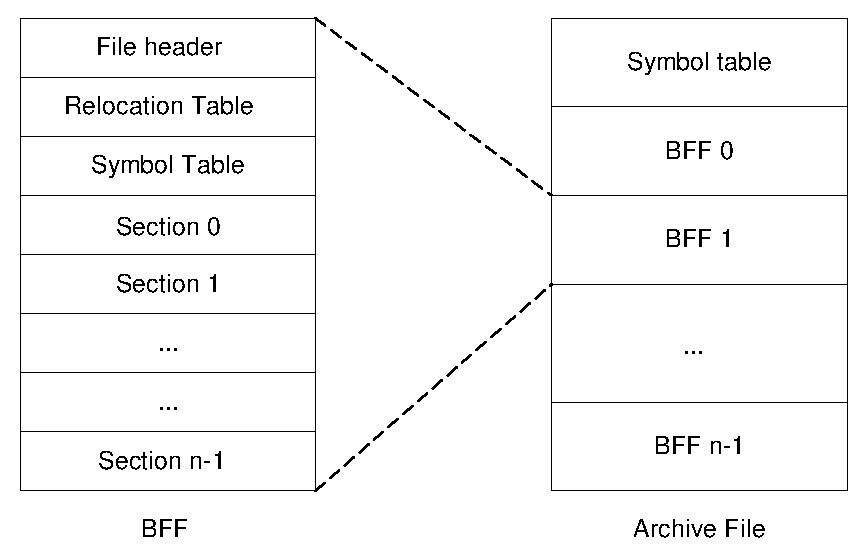
\includegraphics{figures/bffoa.eps}}
\centerfigend{fig-bffoa}{BFF and archive file abstraction}

The current development domain for our tools is based on the Solaris 
ELF~\cite{Sun94m} format, the DOS EXE format~\cite{Dunc88b,Micr96}, 
the Windows (16-bit) NE~\cite{Dunc88b,Micr96} format,
and the Palm OS .prc format~\cite{Tso00}.
Archive files are based on the Unix ar(4) file format.
These formats vary in their degree of complexity and information
stored: the DOS EXE is very simple and limited in structure,
whereas the Solaris ELF format is the most complex, while the Windows
NE is somewhere in between.
The amount of information stored for a simple ``Hello world'' program
varies from format to format.  The DOS EXE format contains a file
header, a relocation table and a single image for both code and data.
The Windows NE version contains most DOS EXE's information plus
additional details such as the resource table, entry table, etc.
The ELF format contains even more information; sections within the 
object file hold information used in dynamic linking: code, data, 
relocation tables, symbol tables, dynamic linking information, etc.
The size in bytes of the binaries for (x86,DOS,EXE), (x86,Windows,NE)
and (Sparc,Solaris,ELF) are 6432, 16384 and 5280 respectively.
It can clearly be seen that although the latter two files are dynamically
linked, their sizes are not necessarily smaller than the static (first)
case.
This is due to the small nature of the example program and the
inclusion of the DOS EXE header information within the NE format.



\section{The BinaryFile Object Hierarchy}
BinaryFile and ArchiveFile are abstract classes; that is, they cannot be
instantiated
directly. The user actually uses classes such as ElfBinaryFile or ExeBinaryFile,
which are derived from the abstract BinaryFile class (see 
Figure~\ref{fig-loadHier}).

% xfig figures exported as eps, portrait, 100% size, displayed at 3.2cm.
\centerfigbegin
\resizebox{!}{3.2cm}
{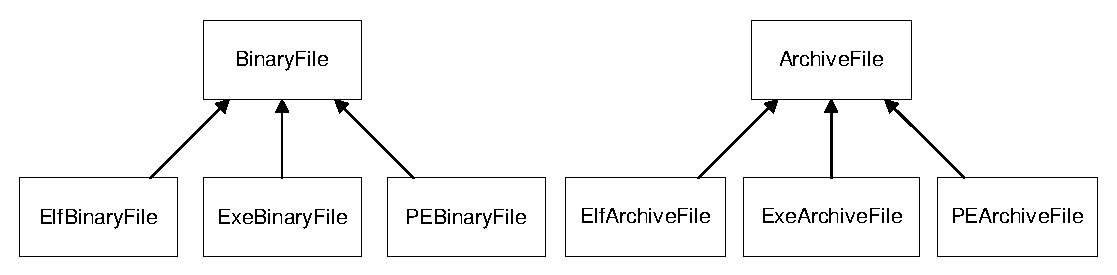
\includegraphics{figures/load_hierarchy.eps}}
\centerfigend{fig-loadHier}{BinaryFile Class Hierarchy}

The user will call functions like \texttt{Load} that are implemented 
differently in the various derived classes. Some functions like
\texttt{SymbolByAddress} are implemented trivially by the BinaryFile class 
(e.g. to always return 0), and this behaviour is overridden by derived 
classes which do the real work.  Even functions like \texttt{GetNumSyms} 
that are implemented by the BinaryFile class will return information that 
will be dependent on the instantiated class.



\section{Interface Functions to Construct and Use a BinaryFile}
The BinaryFile class and each of its parts (described in the abstract 
format description of a binary file in section~\ref{sec-bff}), are 
explained here in terms of interface functions provided for accessing 
information in those parts. 


\subsection{Construction and Loading}
The BinaryFile class provides constructor and destructor 
functions, plus a function to load the binary file.
The loader is an abstract class and hence it does not export 
any types.

\begin{description}
\item [BinaryFile: BOOL $\rightarrow$ BinaryFile].
	This is the constructor. The single BOOL argument is used to
	indicate whether the object to be constructed is to be an
	Archive member; it defaults to false. Users should not use
	this parameter, but should use the ArchiveFile class
	instead (see section~\ref{sec-archive}). The BinaryFile object
	is created without a file loaded; use the Load() function below
	to actually load a file.
	
\item [Load: (BinaryFile x STRING) $\rightarrow$ BOOL].
	Load the given file and store its
	information in a BinaryFile object. It returns whether the
	function was successful or not.
	If there is a problem loading the file, e.g. the file name does
	not exist or there is not enough memory, a message is printed
	on standard error.

\item [UnLoad: BinaryFile $\rightarrow$ nil].
	Deallocates the BinaryFile object. All information about the file
	(e.g. SectionInfo, pointers to section data) are invalid after
	calling this function.

\end{description}


\subsection{Sections}
For each section in the binary file, the following information is 
collected in a SECTIONINFO type:
\begin{itemize}
\item Section name: the name of the section, if any.  Formats like
	ELF support names for each section, such as \texttt{.text} and
    \texttt{.bss}; formats such as EXE do not provide such information
	and hence we follow the convention of naming them \texttt{\.header}
	and \texttt{.text} for the header of the file and the relocatable
	image respectively.

\item Native address: address where the section is logically loaded.
	For example, all EXE files are loaded at address 0x100000,
	representing 10:0000.  ELF files are loaded at the address
	specified in the elf file, typically 0x10000 for code and 0x20000
	for data.  The native address is typically used by diassemblers
	to give a useful address in listing. 

\item Host address: the host address is where the section is actually
	located in virtual memory, i.e. this is a pointer to the first
	byte in the section.

\item Section size: size of the section in bytes.

\item Number of entries: if the section is the equivalent to an 
	array of entries, the size of each entry is given.

\item bCode: This flag is set if the section contains executable
	instructions.

\item bData: This flag is set if the section contains data. It is possible
	for both bCode and bData to be set at the same time.

\item bBss: This flag is set if the section is not initialised, i.e. it
	is for reserving space only.

\item bReadOnly: This flag is set if the section is read only, i.e. it
	cannot be written to.

\end{itemize}

For example, with the ElfBinaryFile class, the section whose name is 
\texttt{\.rodata} would have the flags bData and bReadOnly set.
A disassembler can find all the sections worth disassembling by 
searching through all the sections for those with the flag bCode set.

Sections provide the following functions to determine the number
of sections available in the file and access its information:
\begin{description}
\item [GetNumSections: BinaryFile $\rightarrow$ int].
	Given a BinaryFile object, returns the number of sections that it 
	contains.  

\item [GetSectionInfo: (BinaryFile x int) $\rightarrow$ SECTIONINFO].
	Given an BinaryFile object and a section index, returns the information
	for that section.  Note that sections are indexed from 1.
\end{description}


\subsection{Symbol Table}
Symbol tables are often used for dynamic linking purposes, where
the names of dynamically linked-in routines are stored.  However,
sometimes program symbols are also stored in a symbol table,
whether in the same or a separate table to that of dynamic linking.

The symbol table offered by the BinaryFile class is very simple; 
there are three types of information stored for each entry:
\begin{itemize}
\item Symbol name: the symbol's name in the table.  Type: STRING.

\item Symbol address: the symbol's native address.  Type: ADDRESS.

\item Symbol size: the size in bytes associated with the symbol.
	Type: int.
\end{itemize}

The symbol table offers three access functions to its contents:
\begin{description}
\item [SymbolByAddress: (BinaryFile x ADDRESS) $\rightarrow$ STRING].
	Given a native address, returns the symbolic name associated with the 
	given native address.
	This function is useful when getting names for procedures at
	call locations.

\item [GetAddressByName: (BinaryFile x STRING) $\rightarrow$ ADDRESS].
	Given the name of a symbol, returns the native address associated
	with it.	
	If the symbol is inexistent in the symbol table, an address of 
	0 is returned.

\item [GetSizeByName: (BinaryFile x STRING) $\rightarrow$ int].
	Given the name of a symbol, returns the size in bytes of the 
	symbol, or 0 if inexistent.
\end{description}

Not all BinaryFiles provide the ByName() functions, because in some
cases the binary file format does not support it. If the functions are
not supported, they will always return 0.

Some BinaryFile classes (e.g. ExeBinaryFile) do not implement a symbol table.


\subsection{Relocation Table}
Relocation tables provide information on address that need to be
relocated prior to execution of the program.  
The advantage of knowing which addresses are relocatable is
that when decoding a machine instruction that takes an immediate
operand, we can check if this operand is an address or not. 
This provides us with useful information that is unavailable otherwise.

The functions provided to access the relocation table are:
\begin{description}
\item [IsAddressRelocatable: ADDRESS $\rightarrow$ BOOL].
	Given a native address, returns whether the address is in the
	relocation table or not.

\item [GetRelocatedAddress: ADDRESS $\rightarrow$ ADDRESS].
	Given a native relocatable address, returns the relocated 
	address for it. This function is tentative and not implemented
	as yet; RISC machines require many bit manipulations, and
	this will probably require a different interface function.
\end{description}

With object files, relocations are often associated with symbols.
Sometimes, (e.g. with GCC), intramodule function calls that
could be resolved at compile time are left until link time, so
the call has a relocation entry with an associated symbol table
entry (often not the same symbol table as the main symbols).
To make use of this, the BinaryFile provides this function:

\begin{description}
\item [GetRelocSym: ADDRESS $\rightarrow$ STRING]. Given a
native address, returns a symbol associated with the relocation
at that address, if any. If there is no symbol, the function
returns 0.
\end{description}


\subsection{Program Headers}
Application writers normally like dumping information about 
the headers of the program in order to determine format-specific
information that is not otherwise accessible via the loader
interface.  For example, a loader may have a verbose option to
display this type of information.

Unfortunately, it is difficult to provide a clean interface for
such low level details. (The previous version of the loader
attempted this, but it was not satisfactory). Therefore this
version of BinaryFile provides just one function, for dumping
all the headers in a verbose manner:

\begin{description}
\item [DisplayDetails: BinaryFile x STRING x FILE* $\rightarrow$ BOOL].
	Given a BinaryFile class and the name of the file, sends a verbose
	listing of the
	file to the file indicated by the FILE* parameter.
	The STRING parameter is merely to provide the first line of output,
	which is typically {\it Type} header for {\it Filename}.
	The FILE* parameter can be a special stream such as
	\texttt{stdio}, or a file opened with the \texttt{fopen}
	library function.

\end{description} 

The addresses referred to above are host addresses, i.e. pointers
to actual loaded data. (By contrast, native addresses are those
where part of a file is expected to be loaded in the native
operating system. Headers have no native address.

In the ElfBinaryFile, more specific functions are provided to
access different named headers, such as GetProgramHeader()
and GetSectionHeader().

Given the address of a header, an application writer would have
to know what the contents of the header looks like, and would
have to write the dump function.  We do not consider this
type of detail should be included in our BinaryFile class.


\subsection{Analysis Functions}
The following functions are provided for extra functionality 
required under binary translation, they are:
\begin{description}
\item [GetInitialState: BinaryFile $\rightarrow$ LIST$<$(REGxADDRESS)$>$].
	Returns a list of registers and their initial value (normally
	an address) prior to program execution.

\item [GetEntryPoints: BinaryFile $\rightarrow$ LIST$<$ADDRESS$>$].
	Returns a list of native addresses which are entry points into the 
	program.  The first address is always the initial value of the program
	counter (PC).

\emph{The following function is not implemented at present. It occured to
	me (Mike) that
	the mapping from Native to Host address may vary for each section;
	it doesn't in elf, but it may for other sections. Let's leave this
	one out unless we really need it. It is easy to implement anyway:
	just use the difference between native and host addresses in the
	section info.}
\item [NativeToHostAddress: (BinaryFile x ADDRESS) $\rightarrow$ ADDRESS].
	Given a native address, returns its equivalent host address.
	This function allows access to a block of bytes, since a native
	address is just a pointer.

\item [IsDynamicLinkedProc: (BinaryFile x ADDRESS) $\rightarrow$ BOOL].
	Given a native address, returns whether the address is that of a 
	dynamically linked-in procedure or not in this BinaryFile class.

\item [LoadDynamicLinkedProc: BinaryFile $\rightarrow$ ADDRESS $\rightarrow$ BOOL].
	Given the address of a dynamically linked-in procedure (i.e. the
	target of a call instruction that calls such a function, which
	will usually be an address in the Program Linkage Table), loads
	the appropriate source library file (if needed) to resolve this
	call. It returns its success or otherwise, and the native address
	where the procedure is loaded. 

	There will have to be environment variables to specify what path(s)
	should be searched to locate the appropriate library. These would
	be called \\
	X86\_LIBRARY\_PATH\\
	SPARC\_LIBRARY\_PATH\\
	and so on.  For example,
	if an X86 source program calls the \texttt{atan} function,
	the program's dynamic section specifies the DT\_NEEDED libraries
	as "libc.so.1" and "libm.so.1", and the environment variable
	X86\_LIBRARY\_PATH is set to "/var/lib/x86:/usr/lib/x86", then
	the following libraries will be searched for the \texttt{atan}
	function: \\
	/var/lib/x86/libc.so.1, /var/lib/x86/libm.so.1,
	/usr/lib/x86/libc.so.1, /usr/lib/x86/libc.so.1 \\
	Note that this function is only needed if/when we start supporting
	translations of libraries; at present we assume a native library
	is available.  Hence this function is not implemented at present.
\end{description}



\section{Notes on Individual BinaryFiles}

At present, the ElfBinaryFile is by far the most complete. It is the
only version that implements DisplayDetails(). The need to use
ElfDetails.cc at all, and all the verbose dumping code, can be 
avoided by defining \texttt{NODETAILS} in the make.

The ExeBinaryFile class does not handle symbols (e.g. Microsoft
Codeview or Borland) as these are stored in different ways by
different EXE compilers.

ElfBinaryFile implements symbols, both by address and by name. The
table of symbols looked up by value comes from the \texttt{.symtab}
section, if present, otherwise from the \texttt{.dynsym} section.

When looking up symbols by name, the \texttt{.hash} section is used. This
section refers to the \texttt{.dynsym} section, not the \texttt{.symtab}
section (if present). 
Thus, it is possible to look up local (non dynamic) symbols by value, 
but not by name.  This is a limitation of the way that elf files
are made. 
ElfBinaryFile implements the symbol size field of the SYM\_VALUE passed to 
ValueByName().

Some library files (e.g. libstdc++) have silly dynamic symbol table
entries (that they don't define), with a symbol type of STT\_NOTYPE.
Symbols of this kind are treated as if they don't exist in the symbol
table (i.e. ValueByName() returns 0 for these). 



\section{Interface Functions to Construct and use an ArchiveFile}
\label{sec-archive}

The ArchiveFile class and each of its parts (described in the abstract 
format description of a binary file in section~\ref{sec-bff}), are 
explained here in terms of interface functions provided for accessing 
information in those parts. 

\begin{description}
\item [ArchiveFile: nil $\rightarrow$ ArchiveFile].
	This is the constructor; there are no arguments. The object is
	created without a file being loaded; use the Load function below
	to load an archive file.

\item [Load: STRING $\rightarrow$ BOOL].
	Loads the archive file whose name is given. Returns false if the
	file could not be found, not opened, or it was not an archive
	file. Messages may be displayed on standard error.

\item [UnLoad: ArchiveFile $\rightarrow$ nil].
	Unloads the archive file, and any members that may have been loaded
	and not yet unloaded.  All information about the archive file
	and member files are invalid after calling this function.

\item [GetNumMembers: ArchiveFile $\rightarrow$ int].
	Returns the number of members, not including any special members
	that may exist merely for administrative purposes (e.g. the
	empty members in elf archives that hold the symbol table).

\item [GetMember: ArchiveFile x int $\rightarrow$ BinaryFile*].
	Given an index (0 for first, etc), constructs, loads, and returns
	a pointer to a BinaryFile object for that member. The binaryfile
	object comes pre-loaded; the user should not call the Load function
	for the returned member, but should call UnLoad when done with the
	member object. In the case of errors, a NULL pointer is returned.

\item [GetMemberByProcName: ArchiveFile x STRING $\rightarrow$ BinaryFile*].
	Similar to the above function, except that the relevant member is
	selected by procedure name, e.g. "arctan".

\item [GetMemberByFileName: ArchiveFile x STRING $\rightarrow$ BinaryFile*].
	Similar to the above function, except that the relevant member is
	selected by the name of the archive member (this will usually be an
	object file without an explicit path, e.g. "transcend.o").

\item [GetMemberFileName: ArchiveFile x int $\rightarrow$ STRING].
	Given a member index, return the name of the archive member.


\end{description}

Many of the functions above presume some knowledge of the contents of
the archive, e.g. the file name of the members, or symbols in those
members. There are at present no functions to allow the user to browse
these items.

\section{Example Code}

Examples are often worth a thousand words.  Here are two examples
on how to use the BinaryFile and derived classes.


\subsection{Example 1}
Here is a complete, though simple, program to use the ElfBinaryFile class. 
It simply iterates through the sections of the file, and counts how 
many sections contain code (i.e.  have the ST\_CODE flag set).

\begin{verbatim}
#include <stdio.h>
#include "ElfBinaryFile.h"

int main(int argc, char* argv[])
{
    ElfBinaryFile L;
    int iCnt = 0;

    if (!L.Load(argv[1])) return 1;
    int n = L.GetNumSections();
    PSECTIONINFO pSect = L.GetSectionInfo();
    for (int i=0; i < n; i++)
        if (pSect[i].bCode) iCnt++;
    printf("Part %d has %d code section(s)\n", iPart, iCnt);
    L.UnLoad();
    return 0;
}
\end{verbatim}

This can be compiled as follows (assuming that the above source is in
\texttt{sample.cc}):
\begin{verbatim}
gcc -o sample sample.cc BinaryFile.cc ElfBinaryFile.cc ElfDetails.cc
    SymTab.cc -lelf -lstdc++
\end{verbatim}

The \texttt{"-lelf"} is because ElfBinaryFile requires the elf library; other
versions of the loader would probably not need any libraries other than the
standard template library.
The results are:

\begin{verbatim}
% sample sample
Part 1 has 4 code section(s)

% sample /usr/lib/libelf.a
Part 1 has 1 code section(s)
Part 2 has 1 code section(s)
...
Part 42 has 1 code section(s)
\end{verbatim}


\subsection{Example 2}
The following example dumps the \texttt{\_exit} function
(if present) of the given input file.   Assume the following
code is in file dumptext.cc.

\begin{verbatim}
#include "ElfBinaryFile.h"

int main(int argc, char* argv[])
{
    ElfBinaryFile L;
    SYM_VALUE v;
    PSECTIONINFO pText;

    if (!L.Load(argv[1])) return 1;

    if (L.ValueByName("_exit", &v))
    {
        pText = L.GetSectionInfoByName(".text");
        if (pText)
        {
            int n = v.iSymSize;
            printf("Function _exit (%d bytes):\n", n);
            printf("%08X: ", pText->uNativeAddr);    // Address
            // Compute offset from start of text section to this function
            dword offset = v.uSymAddr - pText->uNativeAddr;
            dword p = pText->uHostAddr + offset;    // Start of function
            for (int i=0; i < n; i++)
                printf("%02X", *((unsigned char*)p++));
            printf("\n");
        }
    }
    else printf("No function '_exit'\n");
    return 0;
}
\end{verbatim}

To compile it, at the command line type:
\begin{verbatim}
gcc -g -o dumpexit dumpexit.cc BinaryFile.cc ElfBinaryFile.cc SymTab.cc 
    ElfDetails.cc -lelf -lstdc++
\end{verbatim}

Sample output: 
\begin{verbatim}
% dumpexit /usr/lib/libc.so.1 
Function _exit (8 bytes):
000169A0: 8210200191D02008
% 
\end{verbatim}

\subsection{Example 3}

The following example loads the archive "/usr/lib/libm.a" and displays
the load address for the "sin" function.

\begin{verbatim}
#include <stdio.h> 
#include "ElfArchiveFile.h"
void main()
{

    ElfArchiveFile af;
    if (!af.Load("/usr/lib/libm.a"))
    {
        printf("ArchiveFile could not load file\n");
        return 1;
    }

    printf("There are %d members in this archive\n", af.GetNumMembers());
    printf("First 5 file names:\n");
    for (int i=0; i < 5; i++)
    {
        printf("%s\n", af.GetMemberFileName(i));
    }

    BinaryFile* pm;
    printf("Object for function 'sin' is at %p\n",
        pm = af.GetMemberByProcName("sin"));
    printf("Address of sin is %p; size %d\n", pm->GetAddressByName("sin"),
        pm->GetSizeByName("sin"));
    pm->UnLoad();

	af.UnLoad();
}
\end{verbatim}

To compile, (assuming the example code is called example3.cc):
\begin{verbatim}
gcc -g -DUNIX -o example3 example3.cc BinaryFile.cc ElfBinaryFile.cc
    SymTab.cc ElfDetails.cc ArchiveFile.cc ElfArchiveFile.cc -lelf -lstdc++
\end{verbatim}


\subsection{Compiling and Linking}
Applications using the BinaryFile class need to compile the files 
\texttt{BinaryFile.cc} and \texttt{ExeBinaryFile.cc} (or \texttt{ElfBinaryFile.cc},
\texttt{PEBinaryFile.cc}, etc).  They should link the resultant object files 
with the application. The final executable must be linked with the standard
template library, e.g. "-lstdc++" for the GCC compiler. Elf versions
also require the elf library, i.e. "-lelf" for GCC.

In addition, BinaryFile classes implementing symbol tables (at present,
this is only the ElfBinaryFile class) also need to compile \texttt{SymTab.cc}
which depends on \texttt{SymTab.h}, and should link with \texttt{SymTab.o}.

For the ElfBinaryFile class, unless \texttt{NODETAILS} is defined in
the make (with \texttt{-DNODETAILS}), the file \texttt{ElfDetails.cc}
must also be compiled and the resultant \texttt{ElfDetails.o} linked.

In those application source files using the BinaryFile class, the appropriate
header file (but not \texttt{BinaryFile.h} itself) should be included. For
example, if using ElfBinaryFile:
\begin{verbatim}
#include "ElfBinaryFile.h"		// Definitions for the ElfBinaryFile class
\end{verbatim}

An example makefile fragment:
\begin{verbatim}
OBJS = myfile1.o ... BinaryFile.o ElfBinaryFile.o SymTab.o ElfDetails.o

ElfBinaryFile.o: BinaryFile.o ElfBinaryFile.h ElfDetails.h

SymTab.o: SymTab.cc SymTab.h

BinaryFile.o: BinaryFile.h
\end{verbatim}



       % binary-file API 

	
\chapter{Decoding of Machine Instructions -- Syntax Parsing}
\label{ch-decoding}

{\small
\begin{flushright}
Design: Cristina; Documentation: Cristina [Feb 00]; Implementation: Cristina, Mike
\end{flushright} 
}


The New Jersey Machine Code (NJMC) toolkit allows users to write
machine descriptions of assembly instructions and their associated
binary representations using the Specification Language
for Encoding and Decoding (SLED).
SLED provides for compact specifications of RISC and CISC 
machines; with 127, 193 and 460 lines of specification for
the MIPS, SPARC and Pentium respectively. 

The toolkit also provides extra support for encoding of assembly to
binary code, and decoding of binary to assembly code.
For decoding purposes, the toolkit provides a \emph{matching} statement 
which resembles the C \texttt{switch} statement.  
The toolkit generates C and Modula-3 code from matching statements, 
hence automating part of the disassembly process.  
The generated code can be integrated as a module of a binary-decoding 
application.  This chapter briefly describes the SLED language, its usage 
for decoding of machine instructions, and the way we have optimised the 
the code that the toolkit generates.


\section{SLED and Decoding of Machine Instructions}
This section provides a brief description of the SLED language in 
order to familiarize the reader with the key concepts of the language.
Readers familiar with the toolkit and its usage should skip this section. 
A full description of the SLED language is provided in~\cite{Rams97}.
A complete description of the usage of the toolkit for both
encoding and decoding purposes is available in the reference 
manual~\cite{Rams94}.


\subsection{SLED Concepts}
SLED introduces the following concepts to describe binary machine
instructions:
\begin{description}
\item [tokens] represent names for a sequence of bits.  Tokens are 
	commonly used to represent the bits of one machine instruction
	or of immediate operands.  A token is given a size, representing
	the number of bits in the token.
\item [fields] describe the parts of a token in terms of their name
	and bit range.  Fields can use little or big endian conventions.
\item [patterns] describe the possible values in the fields of
	a token, and names them.  Pattern names can also refer to groups
	of patterns.
\item [constructors] describe the mapping between binary and a
	symbolic assembly-like representation by associating 
	a list of operands with a pattern.
\item [equations] describe simple mathematical equations which
	place constraints on the values of fields used in constructors.
\item [relocatables] describe operands in constructors that denote 
	relocatable addresses.
\end{description}

A partial example of the SPARC SLED specification is given in
Figure~\ref{fig-sparc-sled}.
The \texttt{fields} keyword describes the specification of
a token named \texttt{instruction} of size 32 bits.  The fields
of that token include: \texttt{op}, \texttt{rd}, and \texttt{rs1}. 
Each field denotes a sequence of bits of the \texttt{instruction} 
token it refers to. 
For example, the \texttt{op} field refers to bits 30 and 31, and
the \texttt{rs1} field refers to bits 14 to 18.   
By default, big-endian convention is used.

\centerfigbegin
\begin{small} 
\begin{verbatim}
fields of instruction (32)
inst 0:31 op 30:31 disp30 0:29 rd 25:29 op2 22:24 imm22 0:21 a 29:29 cond 25:28
disp22 0:21 op3 19:24 rs1 14:18 i 13:13 asi 5:12 rs2 0:4 simm13 0:12 opf 5:13
fd 25:29 cd 25:29 fs1 14:18 fs2 0:4 rs1i 14:18 rdi 25:29

patterns
 [ TABLE_F2 CALL TABLE_F3 TABLE_F4 ] is op  = {0 to 3}
patterns
 [ ADD  ADDcc  TADDcc   WRxxx
   AND  ANDcc  TSUBcc   WRPSR
   OR   ORcc   TADDccTV WRWIM
   XOR  XORcc  TSUBccTV WRTBR
   SUB  SUBcc  MULScc   FPop1
   ANDN ANDNcc SLL      FPop2
   ORN  ORNcc  SRL      CPop1
   XNOR XNORcc SRA      CPop2
   ADDX ADDXcc RDxxx    JMPL
   _    _      RDPSR    RETT
   UMUL UMULcc RDWIM    Ticc
   SMUL SMULcc RDTBR    FLUSH
   SUBX SUBXcc _        SAVE
   _    _      _        RESTORE
   UDIV UDIVcc _        _
   SDIV SDIVcc _        _       ] is TABLE_F3 & op3 = {0 to 63 columns 4}
patterns
  arith   is ADD | ADDcc | ADDX | ADDXcc | TADDcc | TADDccTV |
             SUB | SUBcc | SUBX | SUBXcc | TSUBcc | TSUBccTV |
             MULScc | UMUL | SMUL | UMULcc | SMULcc |
             UDIV | SDIV | UDIVcc | SDIVcc | SAVE | RESTORE

constructors
  imode simm13! : reg_or_imm  is  i = 1 & simm13
  rmode rs2     : reg_or_imm  is  i = 0 & rs2
constructors
  arith rs1, reg_or_imm, rd
relocatable reloc
constructors
  call reloc   { reloc = L + 4 * disp30! } is L: CALL & disp30
\end{verbatim}
\end{small}
\centerfigend{fig-sparc-sled}{Partial SLED specification for the SPARC}

The first \texttt{patterns} keyword defines names for 4 patterns: 
\texttt{TABLE\_F2}, \texttt{CALL}, \texttt{TABLE\_F3}, and 
\texttt{TABLE\_F4}.  Each of these patterns bind to a value of
the \texttt{op} field: \texttt{TABLE\_F2} binds to 0, \texttt{CALL}
binds to 1, \texttt{TABLE\_F3} binds to 2, and \texttt{TABLE\_F4} binds
to 3.  In this way, the 4 main tables described in the SPARC 
manual~\cite{Spar92} can be identified.
The second \texttt{patterns} keyword defines names for each of
the 64 values that the combination of the \texttt{TABLE\_F3} pattern
(i.e. \texttt{op} equal to 2) and the field \texttt{op3} can take.  
Entries labelled \texttt{\_} denote entries without a name; i.e. 
entries that are not defined in the manual.   
The third \texttt{patterns} keyword defines the name \texttt{arith} 
to be any of the patterns in the right-hand side of the \texttt{is} 
keyword; namely \texttt{ADD}, \texttt{ADDcc}, \texttt{TADDcc}, etc.

The first \texttt{constructor} keyword defines the constructor
\texttt{reg\_or\_imm} to be one of two modes: immediate (\texttt{imode})
or register-based (\texttt{rmode}).  The former mode binds 
the value of the \texttt{i} field to 1, and the latter to 0.
The former mode returns the 13-bit value \texttt{simm13} signed-extended 
(the \texttt{!} denotes sign-extension), whereas the latter mode
returns the value of the \texttt{rs2} field (a register number).
The second \texttt{constructor} keyword defines the constructor
\texttt{arith} to require the fields and constructors \texttt{rs1}, 
\texttt{reg\_or\_imm}, and \texttt{rd} (which stand for first register 
operand, second register or immediate operand, and destination register). 
In this definition, it is implied that the bit pattern to be 
matched is that of the pattern \texttt{arith} and the fields
\texttt{rs1}, \texttt{reg\_or\_imm}, and \texttt{rd}.  In other
words, this constructor defines all the arithmetic instructions for
the SPARC. 
The last \texttt{constructor} keyword defines the constructor
\texttt{call}, which takes a relocatable address (denoted by
\texttt{reloc}).  The relocatable address needs to satisfy the
equation \texttt{reloc = L + 4 * disp30!}. 
That is, the relocatable address is equivalent to the sign-extended
(\texttt{!}) 30-bit displacement (\texttt{disp30}) shifted left by 2 
(i.e. a 32-bit address where the least two significant bits are 0) plus 
the current displacement (\texttt{L}).  The value of \texttt{L} is
obtained at runtime, by checking the address at which the 
\texttt{CALL} bit pattern is being decoded from.  The \texttt{call}
constructor is defined as the bit pattern combination of the 
\texttt{CALL} pattern and the \texttt{disp30} field.


\subsection{Decoding Using the New Jersey Machine Code Toolkit}
The NJMC toolkit uses matching statements to drive the decoding
of a binary instruction stream.  A matching statement resembles
a C \texttt{switch} statement, except that only one arm can 
be matched (the first one to be valid in the instruction 
stream). 
A matching statement is identified by the \texttt{match}
keyword.  Arms of the match are identified by the \texttt{|} symbol, 
and the left and right-hand sides of the arm are separated by the 
\texttt{=>} symbol. 
Figure~\ref{fig-matching} provides an EBNF-like specification of
the matching statement.  In that specification, \emph{pc} stands 
for the address to the instruction stream to be decoded, 
\emph{pattern} stands for the SLED pattern to be matched 
(including parameters), \emph{equation} stands for any valid
SLED equation that needs to be valid in conjunction with a 
particular pattern, and \emph{code} stands for the C or Modula3
code that the user wants to associate with the matched pattern.
The keyword \texttt{[name]} is used to return the SLED base
pattern name for the matched pattern. 

\begin{figure}[htb]
\texttt{match} pc \texttt{to} \\
\{\texttt{|} pattern [\{equations\}] [\texttt{[name]}] \texttt{=>} code \} \\
{[\texttt{else} code]} \\
\texttt{endmatch}
{\small \caption{\label{fig-matching}{Matching Statement EBNF Specification}}}
\end{figure}
  
For example, if the patterns \texttt{add} and \texttt{sub} are 
described in a SLED specification for a particular machine, then 
the following matching statement displays those names when matched 
at the binary instruction stream pointed to by the address in \texttt{pc}:
\begin{verbatim}
match pc to
| add (rd, rs1, rs2) => printf ("add\n");
| sub (rd, rs1, rs2) [name] => printf ("%s\n", name);
| else                  printf ("other instruction\n");
endmatch
\end{verbatim}

The ``arguments'' to the constructor are names that match
the field names defined with each constructor (in order of
specification) and return the numerical value of
that field.  Hence, in the above example, \texttt{rd}, 
\texttt{rs1} and \texttt{rs2} are integers.  An application
writer may want to give special semantics to such returned
integers; for example, displaying the name of the register
instead of the integer representation of the register.  If
we assume we have an array of register names called \texttt{reg},
the above example can be re-written to also display the names of the
arguments:
\begin{verbatim}
match pc to
| add (rd, rs1, rs2) => printf ("add %s, %s, %s\n", reg[rd], reg[rs1], reg[rs2]);
| sub (rd, rs1, rs2) [name] => 
                        printf ("%s %s, %s, %s\n", name, reg[rd], reg[rs1], reg[rs2]);
| else                  printf ("other instruction\n");
endmatch
\end{verbatim}

Matching files are processed by the toolkit to generate C or 
Modula-3 code that implements the decoding of the instructions
in the \texttt{match} statement.  

Version 0.5 of the NJMC toolkit makes available an option to
partly automate the generation of a matching statement for a
particular SLED specification.  The option \texttt{-dis} generates
matching statements for the given SLED file(s) and stores them 
in the filename provided:  \\
\hspace*{2cm}\texttt{-dis} filename sledfile(s)\\
In practice, the generated code needs to be modified in order to add 
relevant procedure names for each main matching statement, 
as well as remove duplicated arms from the matching statements.
Note that this option is not currently available in the ML 
version of the toolkit.


\subsubsection{Decoding of RISC Machine Instructions}
Some of the characteristics of RISC machines include the 
orthogonality of their instruction sets and the relatively 
small number of instructions.  Further, the size of each
instruction is fixed and is equivalent to the word size 
of the machine.  These characteristics make the writing
of a SLED spec and decoder easier than for a CISC instruction
set.

Figure~\ref{fig-sparc-decoder} contains a snippet of code
for the SPARC decoder; this code was written by hand rather
than generated automatically.  The main decoding routine is 
\texttt{decode\_instr}, which decodes one instruction per
invocation.  The \texttt{pc} argument points to the address
in memory where the instruction stream to be decoded is located
at.  The \texttt{uNativeAddr} argument contains the native
address where the Elf Loader would be expected to load the
instruction stream, and the \texttt{buf} argument is a buffer
where the textual assembly representation of this instruction
will be stored.  The code in this procedure is straight 
forward, except for the target address of branches and calls.
Other than the type name \texttt{ADDRESS}, all names in uppercase 
represent macros used as a shorthand for invoking functions or 
accessing arrays of strings.

Constructors for branches and calls are defined in the SLED 
spec as using relocatable addresses.  Therefore, the toolkit
generates code to return the relocated target address rather
than the original offset displayed in the instruction.  However,
due to the fact that the toolkit is using the \texttt{pc} address
as the address to relocate from, rather than the \texttt{uNativeAddr}
which it does not know about, the returned target address is 
wrong; hence the use of a simple equation to transform the target
address to the right one.   

\centerfigbegin
{\small
\begin{verbatim}
#define RD   (rd_names[rd])
#define RS1  (rs1_names[rs1])
#define ROI  (dis_roi(roi))
#define ADDR (dis_addr(addr))

char *dis_addr(ADDRESS lc) {
  static char buf[512];
  match lc to
  | indirectA(rs1)   => return RS1;
  | indexA(rs1, rs2) => sprintf(buf, "%s+%s", RS1, RS2);
  | absoluteA(i)     => sprintf(buf, "%d", i);
  | dispA(rs1, i)    => sprintf(buf, "%s%s%d", RS1, (int)i < 0 ? "" : "+", i);
  endmatch
  return buf;
}

char *dis_roi(ADDRESS lc) {
  static char buf[512];
  match lc to
  | imode(i)   => sprintf(buf, "%d", i); return buf;
  | rmode(rs2) => return RS2;
  endmatch
}

void decode_instr (ADDRESS pc, ADDRESS uNativeAddr, char *buf)
{
  match pc to
  | NOP =>          sprintf(buf, "nop");
  | decode_sethi(imm22, rd) =>
                    sprintf(buf, "sethi %%hi(%s), 0x%x", imm22, RD);
  ...
  | alu (rs1, roi, rd) [name] =>
                    sprintf(buf, "%s %s, %s, %s", name, RS1, ROI, RD);
  | branch^a (tgt, a) [name] =>
                    sprintf(buf, "%s 0x%08x (%d) ; a = %d", name,
                           tgt-pc+uNativeAddr, tgt-pc, a);
  | call (tgt) =>   sprintf(buf, "call 0x%08x", tgt-pc+uNativeAddr);
  | JMPL (addr, rd) [name] =>
                    sprintf(buf, "jmpl %s, %s", ADDR, RD);
  ...
  | inst = n =>     sprintf(buf, ".word 0x%08x", n);
  endmatch        
\end{verbatim}
}
\centerfigend{fig-sparc-decoder}{Snippet Code for a SPARC Decoder}

The functions \texttt{dis\_addr} and \texttt{dis\_roi} implement
the matching of an effective address, and a register or immediate 
operand, respectively.  
In the former function, an effective address is defined as being
one of 4 cases, namely, indirect, indexed, absolute, or displacement.
In the latter function, a register or immediate is either of those
two options, which can also be matched against the SLED spec.
Both functions return a buffer with the assembly version of 
the bits matched.

The toolkit provides support for generating the names of registers
based on the names used for patterns in the SLED spec.  In a SLED
spec, any name values given for fields with the \texttt{fieldinfo}
keyword can be retrieved automatically by the toolkit in an array 
of strings.  The command line option \\
\hspace*{2cm}\texttt{-lc-pat-names} \\
generates a header and data declaration file (.h and .c) with the
names of all strings found in a SLED spec.  In our previous 
example, the names for \texttt{rs1\_names} and \texttt{rd\_names} 
were generated by the toolkit in a separate file and imported into
the decoder (aka matcher) file.

In order for the toolkit to fetch instructions from the bit stream
addressed by \texttt{pc} in the previous example, a fetch routine
needs to be provided by the tool writer.  In the case of SPARC, 
all fetches will be 32 bits as all instructions are 32 bits, hence
a \texttt{fetch\_word} function needs to be made available.  Suitable
code for such a function is:
\begin{verbatim}
static ADDRESS fetch_word(ADDRESS lc) {
  return *(ADDRESS *)lc;
}
\end{verbatim}
where \texttt{ADDRESS} is a 32-bit type.  Information about the name
of this function, the type of the address field, and address 
conversions need to be specified in an auxiliary spec.  For the 
SPARC decoder, the interface to the instruction stream is as 
follows:
\begin{verbatim}
address type is "unsigned"
address to integer using "%a"
address add using "%a+%o"
fetch 32 using "fetch_word(%a)"
\end{verbatim} 

Norman believes that in order to get the right relocated address 
out of branches and calls, that the \texttt{address to integer} 
option needs to be changed to something like this: \\ 
\hspace*{2cm}\texttt{address to integer using "\%a - uNativeAddr + pc"} \\
In practice, this has not worked yet, and I have not tried it lately.


\subsubsection{Decoding of CISC Machine Instructions}
Amongst the characteristics of CISC machines are the lack of 
orthogonality in their instruction sets, the large numbers of
machine instructions, and the variable length size for 
instructions.  Further, assembly names are often overloaded.
These characteristics make the writing of SLED specs for CISC
machines harder; nevertheless, the language is expressive 
enough.  

Figure~\ref{fig-cisc-sled} contains part of the SLED code for
the x86 instruction set.  The complexity of the instruction 
set can be seen in terms of the number of different \texttt{field}
definitions, the complex names used to distinguish overloaded
instruction names, and the variety of values available on the
right hand side of constructors.  Further, the addressing modes
(\texttt{Eaddr} and \texttt{Mem}) account for 10 possible 
combinations.

\centerfigbegin
{\small
\begin{verbatim}
fields of opcodet (8) row 4:7 col 0:2 page 3:3
    sr4 3:5 sr16 0:2 r16 0:2 r8 0:2
fields of modrm (8) mod 6:7 reg_opcode 3:5 r_m 0:2
fields of I8   (8) i8  0:7

patterns
arith is any of [ ADD OR
                  ADC SBB
                  AND SUB
                  XOR CMP ], which is row = {0 to 3} & page = [0 1]
[ Eb.Gb Ew.Gw Gb.Eb Gw.Ew AL.Ib AX.Iw ] is col = {0 to 5}

patterns
  arithI    is any of [ ADDi ORi ADCi SBBi ANDi SUBi XORi CMPi ],
            which is (Eb.Ib | Ew.Iw | Ew.Ib); reg_opcode = {0 to 7} ...

relocatable d a
constructors
  Indir    [reg] : Mem { reg != 4, reg != 5 } is mod = 0 & r_m = reg
  Disp8   d[reg] : Mem { reg != 4 }           is mod = 1 & r_m = reg; i8  = d
  Disp32  d[reg] : Mem { reg != 4 }           is mod = 2 & r_m = reg; i32 = d
  Abs32   a      : Eaddr                      is mod = 0 & r_m = 5;   i32 = a
  Reg     reg    : Eaddr                      is mod = 3 & r_m = reg
  Index    [base][index * ss] : Mem { index != 4, base != 5 } is
                        mod = 0 & r_m = 4; index & base     & ss
  Index8  d[base][index * ss] : Mem { index != 4 } is
                        mod = 1 & r_m = 4; index & base     & ss; i8  = d
  Index32 d[base][index * ss] : Mem { index != 4 } is
                        mod = 2 & r_m = 4; index & base     & ss; i32 = d
  ShortIndex    d[index * ss] : Mem { index != 4 } is
                        mod = 0 & r_m = 4; index & base = 5 & ss; i32 = d
  E Mem : Eaddr is Mem

constructors
  arith^"iAL"    i8           is      arith & AL.Ib ; i8
  arith^"iAX"    i16          is      arith & AX.Iw; i16
  arith^"mrb"    Eaddr, reg8! is      arith & Eb.Gb; Eaddr & reg_opcode = reg8 ...
  arith^"mrw"    Eaddr, reg!  is      arith & Ew.Gw; Eaddr & reg_opcode = reg ...
  arith^"rmb"    reg8!, Eaddr is      arith & Gb.Eb; Eaddr & reg_opcode = reg8 ...
  arith^"rmw"    reg!, Eaddr  is      arith & Gw.Ew; Eaddr & reg_opcode = reg ...
  arithI^"wb"    Eaddr, i8!   is      (Ew.Ib; Eaddr) & arithI; i8
  arithI^"b"     Eaddr, i8    is      (Eb.Ib; Eaddr) & arithI; i8
  arithI^"w"     Eaddr, i16   is      (Ew.Iw; Eaddr) & arithI; i16
\end{verbatim}
}
\centerfigend{fig-cisc-sled}{Partial SLED Spec for the x86 Instruction Set}

The partial decoder in Figure~\ref{fig-cisc-decoder} illustrates
matching statements used to decode the x86 instruction set.
The code was mostly generated automatically by the toolkit, with 
manual editing performed in order to remove redundant arms from the 
matching statements, separation of nesting of matching statements, and 
creation of function prototypes.
The matching statement for \texttt{decode\_instr} makes use of 
the optional \texttt{[deltaPC]} notation, the effect of which
is to store the number of bytes that were parsed in the \texttt{deltaPC}
variable.  This is needed by a decoder of CISC instructions as
the instruction length is variable and a multiple of 1 byte.
In the code provided, the address of the host instruction stream
and that of the native address are given in 32-bit quantities, 
which means that 4 bytes can potentially be fetch, although any
one particular instruction may only be 1 or 2 bytes.  We use the
returned \texttt{deltaPC} value to update the host pointer by 
the necessary amount.

Characteristics of the generated code include the abstraction 
of the assembly print and file descriptor used---\texttt{asmprint}
and \texttt{asmprintfd} respectively.  These can be defined in
any suitable way in the tool writer's code; in our case, we defined
them as \texttt{fprintf} and \texttt{stdout} respectively.
The toolkit also generates functions to print signed and unsigned
integer values, dependeing on their size; for example, 
\texttt{print\_signed\_i8} to print an 8-bit signed integer. 
Functions to print registers may depend on the context of 
the instruction; i.e. the register number may be that of a 
byte, 2-byte or 4-byte register, which equates to different 
ascii representation of registers (e.g. \texttt{AL} or \texttt{AX}
or \texttt{EAX}).  In this case, the toolkit generates code to
print the decimal value of the register (i.e. 1, 2 or 4).  
I modified this function manually to display 32-bit registers 
for disassembly purposes -- this code is not correct for all
cases and can be corrected by passing an extra argument to the
print function with the size of the register operand.  
    
\centerfigbegin
{\small
\begin{verbatim} 
#define asmprintf fprintf   // printf function
#define asmprintfd stdout   // print directly to stdout

static void print_Eaddr (unsigned pc) {
    match pc to
    | Abs32 (a) =>
            asmprintf (asmprintfd, "%d", a);
    | E (mem) =>
            print_Mem (mem);
    | Reg (reg) =>
            asmprintf (asmprintfd, "%s", print_unsigned_r32(reg));
    endmatch
}

static void print_signed_reg(int reg) { 
  static char *r32_names[] = {
    "EAX", "ECX", "EDX", "EBX", "ESP", "EBP", "ESI", "EDI",
  };
  asmprintf(asmprintfd, "%s", r32_names[reg]);
//  asmprintf(asmprintfd, "%d", reg);
}

static void print_signed_i8(int /* [-128..127] */ i8) {
  asmprintf(asmprintfd, "%d", i8);
}

unsigned decode_instr (unsigned pc, unsigned uNativeAddr)
{ unsigned deltaPC;     // # of bytes parsed by decoder

  match [deltaPC] pc to
  | ADDrmw(reg, Eaddr) =>
      asmprintf(asmprintfd, "%s", "ADDrmw ");
      print_signed_reg(reg);
      asmprintf(asmprintfd, "%s", ", ");
      print_Eaddr(Eaddr);
  | ADDrmb(reg8, Eaddr) =>
      asmprintf(asmprintfd, "%s", "ADDrmb ");
      print_signed_reg(reg8);
      asmprintf(asmprintfd, "%s", ", ");
      print_Eaddr(Eaddr);
      asmprintf(asmprintfd, "\n");
  | ADDiw(Eaddr, i16) =>
      asmprintf(asmprintfd, "%s", "ADDiw ");
      print_Eaddr(Eaddr);
      asmprintf(asmprintfd, "%s", ", ");
      print_signed_i16(i16);
  | ADDiAL(i8) =>
      asmprintf(asmprintfd, "%s", "ADDiAL ");
      print_signed_i8(i8);
      asmprintf(asmprintfd, "\n");
  ...
  endmatch
  return deltaPC;
}
\end{verbatim}
}
\centerfigend{fig-cisc-decoder}{Snippet Code for an x86 Decoder}

For CISC machines, the toolkit will need to fetch bits in different
byte granularities.  For x86, 1, 2 or 4 bytes may need to be fetched
at any point in time.  This information, along with address information,
is stored in the instruction stream interface file, as follows:
\begin{verbatim}
fetch 8 using "getByte(%a)"
fetch 16 using "get2Bytes(%a)"
fetch 32 using "get4Bytes(%a)"
address type is "unsigned"
address add using "(unsigned)%a + %o"
address to integer using "%a"
\end{verbatim}
And the user is required to provide the implementation for the
functions \texttt{getByte}, \texttt{get2Bytes} and \texttt{get4Bytes}.


\subsection{Cost of Decoding Machine Instructions}
\emph{Some experimentation in this area was done in 
1998 in order to determine bottlenecks in the generated
code and store it in a different way.  The work was 
never finished and neither Norman nor Cristina had
the time to make changes.}

The current NJMC implementation for generating C code from 
matching files is to use a decision tree for all options 
available in a \texttt{match} statement.  In these decision 
trees, every option is inline expanded.  The tree is then
turned into a DAG and only at leaf nodes are \texttt{goto}
statements used.  In the generated code, \texttt{switch}
statements are used for the different options in the decision
tree.

The main problem for performance of the current generated code
seems to be that the code is too large to fit into the icache. 
This implies that there is too much inlining being done in the
code.  Possible optimizations that can be done to reduce this
penalty are:
\begin{itemize}
\item recognize common subexpressions and create procedures for them,
\item convert some of the \texttt{switch} statements into 
      table-driven lookup statements, and 
\item choose an appropriate numbering scheme to eliminate the 
      table lookup (e.g. $\lambda x \bullet x$ or 
      $\lambda x \bullet x \ll 20 \, | \, 17$) in order to cheaply
      compute the equivalent table lookup. 
\end{itemize}

In the case of SPARC, the table-driven implementation may
look like a small decision tree (with 4 branches for the 
main 4 cases, and one of them with extra branches), and 
decision tables for the $n$ decision trees removed. 


\section{Recovery of Jump Table Case Statements from Binary Code}

One of the fundamental problems with the analysis of binary  
(executable) code is that of recognizing, in a machine-independent way,
the target addresses of n-conditional branches implemented via a jump 
table.  Without these addresses, the decoding of the machine 
instructions for a given procedure is incomplete,
leading to imprecise analysis of the code.

The standard method of decoding machine code involves following
all reachable paths from the entry point~\cite{Site93,Cifu95}.
This method does not give a complete coverage of the text space
in the presence of indirect transfers of control such as indexed
jumps and indirect calls.  A common technique used to overcome
this problem is the use of patterns.  A pattern is generated
for a particular compiler to cater for the way in which the
compiler, or family of compilers, generate code for an indexed jump.
This technique is extensively used as most tools deal with a
particular set of compilers; for example, TracePoint only processes
Windows binaries generated by the Microsoft C++ compiler~\cite{Trac97}.
In the presence of optimized code, patterns do not tend to work
very effectively, even when the code is generated by a compiler
known to the pattern recognizer.

In this section we discuss our technique for recovering
jump tables and their target addresses in a machine and compiler
independent way.  The technique is based on slicing and copy
propagation.  The assembly code of a procedure that contains an
indexed jump is transformed into a normal form which allows us to
determine where the jump table is located and what information it 
contains (e.g. offsets from the table or absolute addresses).

The presented technique has been implemented and tested on SPARC and 
Pentium code generated by C, C++, Fortran and Pascal compilers.
Our tests show that up to 90\% more of the code in a text segment can
be found by using this technique, when compared against the 
standard method of decoding.
The technique was developed as part of our resourceable and retargetable 
binary translation framework UQBT; however, it is also suitable for other
binary-manipulation and analysis tools such as binary profilers, 
instrumentors and decompilers.


\subsection{Compiler Code Generation for N-Conditional Branches}
\label{sec-codegen}

N-conditional branches were first suggested by Wirth and Hoare in
1966~\cite{Wirt66,Wran74} as a useful extension to the Algol language.
An n-conditional branch allows a programming language to determine
one of $n$ branches in the code.
This extension was implemented in Algol 68 in a form that allowed
its use as a statement or an expression.  In other words,
the result of the \texttt{case} statement could be assigned to a variable.
This high-level statement has evolved to the well known \texttt{switch}
statement in C and the \texttt{case} statement in Pascal, where labels
are used for the different arms of the conditional branch, and a
default arm is allowed, as per Figure~\ref{fig-eg}.  The C code
shows the indexed variable \texttt{num} which is tested against the values
in the range 2 to 7 for individual actions, and if not successful,
defaults to the last \texttt{default} action.

\centerfigbegin
\begin{small}
\begin{verbatim}

#include <stdio.h>
int main()
{ int num;
    printf("Input a number, please: ");
    scanf("%d", &num);
    switch(num) {
        case 2:
            printf("Two!\n"); break;
        case 3: 
            printf("Three!\n"); break; 
        ...
        case 7:
            printf("Seven!\n"); break;
        default:
            printf("Other!\n"); break;
    }
   return 0;
}
\end{verbatim}
\end{small}
\centerfigend{fig-eg}{Sample switch program written in the C language.}

Although not commonly documented in compiler textbooks, compiler
writers generate different types of machine code for n-conditional
branches.  These ways of generating n-conditional branches are
determined by talking to compiler writers or reverse engineering
executable code.  Several techniques for generating n-conditional branches
from a compiler were documented in the 1970s and 1980s, when optimization 
for space and speed was an important issue.
The most common techniques are described here based on~\cite{Sale81}.

The simplest way of generating code for an n-conditional branch is
as a {\em linear sequence} of comparisons against each arm in the
statement.  This form is efficient for a small number of arms,
typically 4 or less.
A more sophisticated technique is the {\em if-tree}, where the
selection is accomplished by a nested set of comparisons organized
into a tree.
The most common implementation is a {\em jump table}, which may
hold labels or offsets from a particular label.   This implementation
requires a range test to determine the membership of values on
the table.  Although jump tables are the fastest method when there
are many arms in the n-conditional branch, jump tables are space-wise
inefficient if the case values are sparse.
In such cases, a search tree is the most convenient implementation.
When the arms of the n-conditional branch are sparse but yet can
be clustered in ranges, a common technique used is to combine
search trees and jump tables to implement each cluster of
values~\cite{Henn82,Fras91}.
This section deals with the issue of recovering code from generated
\emph{jump tables}, in such a way that the target addresses of an
indexed jump are determined.
%This paper does not attempt to recover high-level n-conditional 
%branch statements, but rather the information necessary to translate 
%an indirect branch indexing a jump table.

For an n-conditional branch implemented using a jump
table, an indexed table is set up with addresses or offsets for each
of the cases of the branch.  The table itself is located in a read-only
data section, or mixed in with the text section.
In the interest of efficiency, range tests for such jump tables
need to be concise.  The most common way of doing both tests is as
follows~\cite{Bern85}:

\begin{small}
\begin{verbatim}
  k <- case_selector - lower_bound
  compare k with (upper_bound - lower_bound)
  if unsigned_greater goto out_of_range
  assertion: lower_bound <= case_selector <= upper_bound
\end{verbatim}
\end{small}

If the case selector value is within the bounds of the upper and
lower bounds, an offset into the jump table is calculated based on
the size of each entry in the table; typically 4 bytes for a 32-bit machine.
Based on the addressing modes available to a machine, either an
indirect jump on the address of the table plus the offset, or an
indexed jump on the same values is generated.  The machine then
continues execution at the target of the indirect/indexed jump. 

Retargetable compilers also use these techniques.  A brief
description for the code generation of an indirect jump through
a jump table for a retargetable C compiler is given in~\cite{Fras95}
by the following specification:

\begin{small}
\begin{verbatim}
if t1 < v[l] goto lolab  ; l=lower bound
if t1 > v[u] goto hilab  ; u=upper bound
goto *table[t1-v[l]]
\end{verbatim}
\end{small}

Overall, compiler writers use a variety of heuristics to determine
which code to generate for a given n-conditional branch based on
the addressing modes and instructions available on the target machine.
It is also common for a compiler to have more than one way of emitting
code for such a construct, based on the number of arms in the
conditional branch and the sparseness of the values in such arms.


\subsection{Examples of Existing Indexed Jumps in Binary Code}
\label{sec-egs}

We present examples of Pentium and SPARC code that
make use of jump tables.  The examples aim to familiarize
the reader with a variety of ways of encoding an n-conditional branch in
assembly code, as well as to show the degree of complexity of such code.
The assembly code for the examples was generated by the Unix
utility \texttt{dis}.  This disassembler uses the convention of
placing the destination operand on the right of the instruction.
The examples show annotated native Pentium and SPARC assembly code, 
and where relevant, the address for the assembly instructions or the 
indexed table.  The annotations were included in these examples 
for ease of readability; they are not part of the produced disassembly. 

\centerfigbegin
\begin{small}
\begin{verbatim}

movl -8(%ebp),%eax           ! Read index variable
subl $0x2,%eax               ! Minus lower bound
cmpl $0x5,%eax               ! Check upper bound
ja   0xffffffd9 <80489dc>    ! Exit; out of range
jmp  *0x8048a0c(,%eax,4)     ! Indexed, scaled jump

8048a0c:  64 89 04 08        ! Table of addresses
8048a10:  78 89 04 08        ! to code handling
8048a14:  8c 89 04 08        ! the various switch
8048a18:  a0 89 04 08        ! cases
...
\end{verbatim}
\end{small}
\centerfigend{fig-eg1}{Pentium assembly code for sample switch program, 
	produced by the Sun cc compiler.}

\centerfigbegin
\begin{small}
\begin{verbatim}

ld    [%fp - 20], %o0        ! Read index variable
add   %o0, -2, %o1           ! Minus lower bound
cmp   %o1, 5                 ! Check upper bound
bgu   0x10980                ! Exit if out of range
sethi %hi(0x10800), %o0      ! Set table address
or    %o0, 0x108, %o0        ! (continued)
sll   %o1, 2, %o1            ! Multiply by 4
ld    [%o0 + %o1], %o0       ! Fetch from table
jmp   %o0                    ! Jump
nop

10908:  0x1091c              ! Table of pointers
1090c:  0x10930
10910:  0x10944
10914:  0x10958
...
\end{verbatim}
\end{small}
\centerfigend{fig-eg2}{SPARC assembly code for sample switch program, 
	produced by the Sun cc compiler.}

The first two examples in Figures~\ref{fig-eg1} and \ref{fig-eg2}
were generated by the \texttt{cc} compiler on a Solaris Pentium and
SPARC machine respectively, from the sample program in Figure~\ref{fig-eg}. 
In Figure~\ref{fig-eg1}, register \texttt{eax} is used as the index
variable; its value is read from a local variable on the stack
(\texttt{[ebp-8]}, the case selector).  The lower bound and the range 
of the table are checked (2 and 5 respectively); the code exits if the value
of the index  variable is out of bounds.  If within bounds,
an indexed scaled jump on (\texttt{eax*4}) is performed, offset from
the start of the indexed table at \texttt{0x8048a0c}.
The contents of the values of the table are of addresses; each is
displayed in little-endian format.

Figure~\ref{fig-eg2} performs the same logical steps as Figure~\ref{fig-eg1}
using SPARC assembly code, where indexed jumps do not exist but indirect
jumps on registers are allowed.
In the example, the indexed variable is initially in \texttt{o0}, which
gets set from a local variable on the stack (\texttt{[fp-20]}, the case
selector).
The lower bound is computed and the indexed variable is set to \texttt{o1}.
The range of the table is checked; if out of bounds, the code exits to
address \texttt{0x10980}.  If within bounds, the address of the table
is computed to \texttt{o0} (by the \texttt{sethi} and \texttt{or}
instructions), the indexed register is multiplied by 4 to get the
right 4-byte offset into the indexed table, and the value of the
table (\texttt{o0}) indexed at \texttt{o1} is fetched into \texttt{o0}.
A jump to \texttt{o0} is then performed.

\centerfigbegin
\begin{small}
\begin{verbatim}

18524:  ld           [%fp - 20], %o0   ! Read indexed variable
18528:  sub          %o0, 67, %o0      ! Subtract lower bound
1852c:  cmp          %o0, 53           ! Compare with range-1
18530:  sethi        %hi(0x18800), %o2 ! Set upper table addr
18534:  bgu          0x18804           ! Exit if out of range
18538:  nop
1853c:  or           %o2, 108, %o2     ! Set lower table addr
18540:  srl          %o0, 4, %o1       ! Hash...
18544:  sll          %o1, 1, %o1       ! ...
18548:  add          %o1, %o0, %o1     ! ...function
1854c:  and          %o1, 15, %o1      ! Modulo 16
18550:  sll          %o1, 3, %o4       ! Multiply by 8
18554:  ld           [%o4 + %o2], %o3  ! First entry in table
18558:  cmp          %o3, %o0          ! Compare keys
1855c:  be           0x1885c           ! Branch if matched
18560:  cmp          %o3, -1           ! Unused entry?
18564:  be           0x18804           ! Yes, exit
18568:  nop                            ! (delay slot)
1856c:  add          %o4, 8, %o4       ! No, linear probe
18570:  and          %o4, 120, %o4     ! with wraparound
18574:  ba           0x18554           ! Continue lookup
18578:  nop

1885c:  add          %o4, %o2, %o4     ! Point to first entry
18860:  ld           [%o4 + 4], %o0    ! Load second entry
18864:  jmp          %o0               ! Jump there
18868:  nop

! Each entry is a (key value, code address) pair
1886c:  0x0
18870:  0x187b4         ! Case 'C'+0
18874:  0xffffffff      ! Unused entries have -1 (i.e. 0xffffff) as 
                        ! the first entry
18878:  0x18804         
1887c:  0x10
18880:  0x185b8         ! Case 'C'+0x10 = 'S'
18884:  0x2f
18888:  0x18630         ! Case 'C'+0x2f = 'r'
...
\end{verbatim}
\end{small}
\centerfigend{fig-eg3}{SPARC assembly code from the vi program, produced
	by the Sun cc version 2.0.1 compiler.}

Figure~\ref{fig-eg3} presents a SPARC example that uses a hash function
to determine how to index into the table.  The code comes from the
Solaris 2.5 \texttt{vi} program.  The index variable is set as \texttt{o0},
and it is normalized by subtracting its lower bound.  The range of
the table is checked; if the value is out of range, a jump to the
end of the case statement is performed (\texttt{0x18804}).
If within bounds, the table's address is set in register \texttt{o2}.
The indexed register is hashed into \texttt{o1} and multiplied by
8 (into \texttt{o4}) to get the right offset into the table (as the
table contains two 4-byte entries per case).
A word is loaded from the table into register \texttt{o3} and its
value is compared against the hash function key (the normalized
index variable \texttt{o0}).  If the
value matches, the code jumps to address \texttt{0x1885c}, where
a second word is read from the table into \texttt{o0}, and a register
jump is performed to that address.
In the case where the value fetched from the table does not match the
key, an end-of-hashing comparison is performed against the value
\texttt{-1}.
If \texttt{-1} is found, the code exits (\texttt{0x18804}), otherwise, the
indexed register (\texttt{o4}) is set to point to the next value
in the table (wrapping the offset into the table from the end
of the table to the start) and the process is repeated at
address \texttt{0x18554}.
Note that this table contains 2 entries per case; the first one
is the normalized index value, and the second one is the target address for
the code associated with that case entry. 

\centerfigbegin
\begin{small}
\begin{verbatim}

8057d90:  movb   38(%eax),%al       ! Get struct member
8057d93:  testb  $0x2,%al           ! Test bit
8057d95:  setne  %edx               ! To boolean
8057d98:  andl   $0xff,%edx         ! To byte
8057d9e:  testb  $0x4,%al           ! Test another bit
8057da0:  setne  %ecx
8057da3:  andl   $0xff,%ecx         ! Save in cl
8057da9:  testb  $0x8,%al           ! Test third bit
8057dab:  setne  %eax
8057dae:  andl   $0xff,%eax         ! Save in al
8057db3:  shll   $0x2,%edx          ! To bit 2 
8057db6:  shll   %ecx               ! To bit 1 
8057db8:  orl    %edx,%ecx          ! Combine these two  
8057dba:  orl    %eax,%ecx          ! Combine all three
8057dbc:  cmpl   $0x7,%ecx          ! Upper bound compare
8057dbf:  jbe    0x280 <8058045>    ! Branch if in range
...
8058045:  jmp    *0805f5e8(,%ecx,4) ! Table jump 
...
805f5e8:  f8 7d 05 08               ! table of addresses of code to 
805f5ec:  01 80 05 08               ! handle switch cases
...                    
\end{verbatim}
\end{small}
\centerfigend{fig-eg4}{Pentium assembly code from the m88ksim program, produced
	by the Sun cc version 4.2 compiler.}

Our last example, Figure~\ref{fig-eg4}, is from the \texttt{m88ksim} 
SPEC95 benchmark suite.  This example shows 3 groups of tests on bits of a
field within a structure, which get stored in registers \texttt{edx},
\texttt{ecx} and \texttt{eax}.  The three partial results are
then or'd together to get the resultant indexed variable in register
\texttt{ecx}.  The upper bound is checked (7) and, if within bounds,
a branch to address \texttt{0x8058045} is taken, where an
indexed branch is made on the contents of register \texttt{ecx}, scaled 
by the right amount (4), and the table address.
Note that the branch (\texttt{jbe}) is the opposite of that
normally found in \texttt{switch} statements (i.e. \texttt{ja}).
This illustrates the danger of relying on patterns of instruction
to recover indexed branch targets; such a piece of code could not
be well specified in a pattern.  For the interested reader, this 
code was produced from the C macro in Figure~\ref{fig-eg4'}.
The appendix illustrates more examples.

\centerfigbegin
\begin{small}
\begin{verbatim}

#define FPSIZE(ir)    ((((ir->p->flgs.dest_64) ? 1 : 0) << 2) | \
                      (((ir->p->flgs.sl_64) ? 1 : 0) << 1) | \
                      ((ir->p->flgs.s2_64) ? 1 : 0))

    switch (FPSIZE(ir)) {
      case SSS: /* other code */
      /* other cases */
    }
\end{verbatim}
\end{small}
\centerfigend{fig-eg4'}{C source code for example in Figure~\ref{fig-eg4}}


\subsection{Our Technique}
\label{sec-tech}
We have developed a technique to recover jump table branches
from disassembled code.  The technique is architecture, compiler
and language independent, and has been tested on CISC and RISC
machines with a variety of languages and compilers (or unknown
compiler, when dealing with precompiled executables).
Development of general techniques is an aim in our work as analysis
of executable code should not rely on particular compiler
knowledge; this knowledge prevents the techniques from working with
code generated by other compilers, and in most cases, for other
machines.

There are 3 steps to our technique:
\begin{enumerate}
\item Slice the code at the indexed/indirect register jump,
\item Perform copy propagation to recover pseudo high-level
	statements, and
\item Check against indexed branch normal forms to determine
	the type of jump table.
\end{enumerate}


\subsubsection*{Slicing of Binary Code}
\label{sec-slice}
Our executable code analysis framework allows for the disassembly
of the code into an intermediate representation composed of
register transfer lists (RTL)~\cite{Cifu98c} and control
flow graphs for each decoded procedure in the program.
The RTL describes the effects of machine instructions in terms of register
transfers, and is general enough to support RISC and CISC machine
descriptions.

When an indexed or indirect jump is decoded, we create an intraprocedural
backward slice of the disassembled binary code~\cite{Cifu97d}.
Slicing occurs by following the transitive closure of registers
and condition codes that are used in a given expression.
The stop criterion for a given register along a path is when that
register is loaded from memory (i.e. from a local variable, a
procedure argument, or a global variable), it is returned by another
function, or it reaches the start of the procedure without being defined
(and hence it is a register parameter set by the caller).

For the purposes of determining jump tables, we have an
extra stop criterion: if the lower bound of the indexed jump is
found, and other relevant information has been found, no more slicing 
is performed.
Of course, this condition is not always satisfied as indexed tables
whose first entry corresponds to the register being zero do not need 
to check for the lower bound.  In such cases,
the slice finishes by means of the other stop conditions.
In the case of slices across calls, we stop if the register is
returned by the call (i.e. \texttt{eax} on Pentium or \texttt{o0} on
SPARC); in other cases we assume registers are preserved across
calls and continue slicing.  This is a heuristic that works well
in practice and is used rarely.  The heuristic
works when the machine code conforms to the operating system's
application binary interface~\cite{Unix90}.

For example, for Figure~\ref{fig-eg1}, the following slice is
created using RTL notation:

\begin{small}
\begin{verbatim}
(1)  eax = m[ebp-8]
(2)  eax = eax - 2
(3)  ZF = (eax - 5) = 0 ? 1 : 0
(4)  CF = (~eax@31 & 5@31) | ((eax-5)@31 & (~eax@31 | 5@31))
(5)  PC = (~CF & ~ZF) = 1 ? <exit> : <step 6> 
(6)  PC = m[0x8048a0c + eax * 4] 
\end{verbatim}
\end{small}
Register \texttt{ebp} points to the stack, therefore indexed variable
\texttt{eax} fetches a value from the local memory for that procedure.
The indexed register is normalized by subtracting the lower bound (2)
and its range is checked against 5 (the difference between the upper
and lower bounds).  If within bounds, an indexed jump is performed 
at statement 6.

In our implementation, when the slice reaches a subtraction, it is assumed
that the subtraction is defining the lower bound of the switch variable's
values.

\subsubsection{Copy Propagation}
Once a slice has been computed, we perform copy propagation
on registers and condition codes.  This is a common technique
used in reverse engineering when recovering higher-level statements
from more elementary ones, such as assembly code~\cite{Cifu96,Cifu98h}
and COBOL code~\cite{Huan98}.

As per \cite{Cifu98h}, a definition of a register $r$ at instruction $i$
in terms of a set of $a_k$ registers, $r = f_1(\{a_k\},i)$, can be copy 
propagated at the use of that register on another instruction
$j$, $s = f_2(\{r,\ldots\},j)$, if the definition at $i$ is
the unique definition of $r$ that reaches $j$ along all paths in
the program, and no register $a_k$ has been redefined along that
path.  The resulting instruction at $j$ would then look as follows: 

\hspace*{2cm}  $s = f_2(\{f_1(\{a_k\},i),\ldots\},j)$   

and the need for the instruction at $i$ would disappear.
The previous relationship is partly captured by the definition-use (du)
and use-definition (ud) chains of an instruction: a use of a register is
uniquely defined if it is only reached by one instruction, that is,
its ud chain set has only one element.
This relationship is known as the $r\mbox{-clear}_{i \rightarrow j}$
relationship for register $r$.  More formally,

$$
\begin{array}{ll}
s = f_2(\{f_1(\{a_k\},i),\ldots\},j) \mbox{ iff } & |ud(r,j)| = 1 \, \wedge \\
  & ud(r,j)=i \  \wedge \\
  & j \in du(r,i) \, \wedge \\
  & \forall a_k \, \bullet \, a_k\mbox{-clear}_{i \rightarrow j} \\
\end{array}
$$

Note that this definition does not place a restriction on the
number of uses of the definition of $r$ at $i$.  Hence, if the
number of elements on $du(r,i)$ is $n$, instruction $i$ can
potentially be substituted into $n$ different instructions $j_k$,
provided they satisfy the $r\mbox{-clear}_{i \rightarrow j_k}$
property.

In our example of Figure~\ref{fig-eg1}, the application of
copy propagation to the slice found in Section~\ref{sec-slice}
gives the following pseudo high-level statements:

\begin{small}
\begin{verbatim}
(3)  jcond ([ebp-8] > 7) <exit>
(4)  jmp [0x8048a0c + ([ebp-8] - 2) * 4]
\end{verbatim}
\end{small}

where \texttt{jcond} stands for conditional jump and \texttt{jmp} 
stands for unconditional jump.  Statement 3 checks if the case
selector is outside the bounds of the jump, and statement 4 
performs a jump to the content (i.e. an address) of memory location 
\texttt{0x8048a0c + ([ebp-8] - 2) * 4}.  


\subsubsection{Normal Form Comparison}
Our previous example can be rewritten in the following way: 

\hspace*{0.5cm} jcond (var $>$ num$_u$) X  \\
\hspace*{0.5cm} jmp [T + (var - num$_l$) * w] 

where var is a local variable, for example \texttt{[ebp-8]},
num$_u$ is the upper bound for the n-conditional branch, for example 
\texttt{7}, num$_l$ is the lower bound of the n-conditional branch,
for example \texttt{2}, T is the indexed table's address (and
is of type address), for example \texttt{0x8048a0c}, and w is
a constant equivalent to the size of the word of the machine; 4 in
this example.
Based on this information, we can infer that the number of elements
in the indexed table is num$_u$ - num$_l$ + 1, for a total of 6 in the
example.  The example also shows that the elements of the indexed table 
are labels (i.e. addresses) as the jump is to the target address loaded
from the address at {\small \texttt{0x8048a0c + ([ebp-8] - 2) * 4} }.

\centerfigbegin
{\small
\begin{tabular}{|l|l|l|} \hline
Type 	& Normal Form	& Types of $<$expr$>$ allowed \\ \hline
A		& jcond (r[v] $>$ num$_u$) X
		& {r[v]} \\
		& jmp [T + $<$expr$>$ * w]
		& {r[v] - num$_l$} \\
		&						
		& {((r[v] - num$_l$) $<<$ 24) $>>$ 24)} \\ \hline
O		& jcond (r[v] $>$ num$_u$) X
		& {r[v]} \\
		& jmp [T + $<$expr$>$ * w] + T \emph{or}
		& {r[v] - num$_l$} \\
		& jmp PC + [PC + ($<$expr$>$ * w + k)]
		& {((r[v] - num$_l$) $<<$ 24) $>>$ 24)} \\ 
		& jmp PC + [PC + ($<$expr$>$ * w + k)] + k 
		& {((r[v] - num$_l$) $<<$ 24) $>>$ 24)} \\ \hline
H		& jcond (r[v] $>$ num$_u$) X
		& {((r[v] - num$_l$) $>>$ s) + }  \\
		& 
		& {(r[v] - num$_l$)} \\
		& jmp [T + (($<$expr$>$ \& mask) * 2*w) + w]
		& {((r[v] - num$_l$) $>>$ 2*w) + }  \\ 
		&
		& {((r[v] - num$_l$) $>>$ 2) + }  \\
		&
		& {(r[v] - num$_l$)} \\ \hline
\end{tabular}
}
\centerfigend{fig-nf}{Normal forms for n-conditional code after analysis}

The previous example only shows one of several normal forms that
are used to encode n-conditional branches using a jump table.  
We call the previous normal form type A.
Figure~\ref{fig-nf} shows the 3 different normal forms that
we have identified in executable code that runs on SPARC and Pentium.
Normal form A (address) is for indexed tables that contain labels as
their values.
Normal form O (offset) is for indexed tables that contain offsets from
the start of the table $T$ to the code of each case.
Normal form H (hashing) contains labels or offsets in the indexed table.
Form O can also be found in a position independent version as well.
Normal form H contains pairs ($<$value$>$,$<$address$>$) at each entry into
the jump table.

In our 4 examples of Figures~\ref{fig-eg1} to \ref{fig-eg4}, we find
the following normal forms, respectively:

\begin{itemize}
\item {\small \begin{verbatim}
jcond (r[24] > 5) 0x80489dc
jmp [0x8048a0c + (r[24] * 4)]
	\end{verbatim} 
	$\Rightarrow$ normal form A}

\item {\small \begin{verbatim}
jcond (r[9] > 5) 0x10980
jmp [0x10908 + (r[9] * 4)]
	\end{verbatim} 
	$\Rightarrow$ normal form A}

\item {\small \begin{verbatim}
jcond ((r[8] - 67) > 53) 0x18804
jmp [0x1886c + (((((((r[8] - 67) >> 4) << 1) + (r[8] - 67)) & 15) << 3)]
	\end{verbatim} 
	$\Rightarrow$ normal form H}

\item {\small \begin{verbatim}
jcond (((al < 2 ? 1:0) & 0xff) << 2 | ((al < 4 ? 1:0) & 0xff) << 1 |
       ((al < 8 ? 1:0) & 0xff) > 7) 0x8057dc5
jmp [0x805f5eb + (((al < 2 ? 1:0) & 0xff) * 4 | ((al < 4 ? 1:0) & 0xff) * 2 |
     ((al < 8 ? 1:0) & 0xff)) * 4]
	\end{verbatim} 
	$\Rightarrow$ normal form A}
\end{itemize}

Examples of form O are given in the appendix to this chapter.


\subsection{Experimental Results}
\label{sec-results}

We tested the technique for recovery of jump table branches  
on Pentium and SPARC binaries in a Solaris environment.  The following 
integer SPEC95 benchmark programs were used for testing:
\begin{itemize}
\item go: artificial intelligence; plays the game of Go
\item m88ksim: Motorola 88K chip simulator; runs test program
\item gcc: GNU C compiler; builds SPARC code
\item compress: compresses and decompresses a file in memory
\item li: LISP interpreter
\item ijpeg: graphic compression and decompression
\item perl: manipulates strings (anagrams) and prime numbers in Perl
\item vortex: a database program
\end{itemize}
All benchmark programs were compiled with the Sun cc compiler
version 4.2 on a Solaris 2.6 machine using standard SPEC optimizations 
(i.e. -O4 on SPARC and -O on Pentium). 
We also include results for the \texttt{awk} script interpreter
utility, and the \texttt{vi} text editor (on both Solaris 2.5 and
2.6).  These programs are part of the Unix OS.

\centerfigbegin
{\small
\begin{tabular}{|l|l|l|l|c|} \hline
Benchmark 	& A		& O		& H		& Unknown \\ \hline
awk 		& 0		& 2		& 0		& 0 \\
vi (2.5)	& 10 	& 1 	& 9		& 0 \\
vi 			& 0		& 13	& 0		& 1 \\
go			& 0		& 5		& 0		& 0 \\
m88ksim		& 0		& 10	& 0		& 2 \\
gcc			& 0		& 153	& 0		& 1 \\
compress	& 0		& 0		& 0		& 0 \\
li			& 0		& 3		& 0		& 0 \\
ijpeg		& 0		& 3		& 0		& 1 \\
perl		& 0		& 32	& 0		& 0 \\
vortex		& 0		& 21	& 0		& 0 \\ \hline
total		& 10 	& 243 	& 9 	& 5 \\ \hline
\end{tabular}
}
\centerfigend{fig-benchSparc}{Number of indexed jumps for SPARC
	benchmark programs}

\centerfigbegin
{\small
\begin{tabular}{|l|l|l|l|c|} \hline
Benchmark 	& A		& O		& H		& Unknown \\ \hline
awk 		& 6		& 0		& 0		& 0 \\
vi 			& 12	& 0		& 0		& 2 \\
go			& 5		& 0		& 0		& 0 \\
m88ksim		& 17	& 0		& 0		& 0 \\
gcc			& 207	& 0 	& 0		& 5 \\
compress	& 0		& 0		& 0		& 0 \\
li			& 3		& 0		& 0		& 0 \\
ijpeg		& 7		& 0		& 0		& 0 \\
perl		& 36	& 0		& 0		& 1 \\
vortex		& 13	& 0		& 0		& 6 \\ \hline
total		& 306 	& 0 	& 0 	& 14 \\ \hline
\end{tabular}
}
\centerfigend{fig-benchPentium}{Number of indexed jumps for Pentium
	benchmark programs}

Figure~\ref{fig-benchSparc} and \ref{fig-benchPentium} show the
number of indexed jumps found in each benchmark program,
the classification of such indexed jumps into the 3 normal
forms (A, O and H), and any unknown types.
In the case of SPARC code, most indexed jump tables are of form
O, which means that the indexed table stores offsets from the
start of the table to the destination target address.
In the case of Pentium code, almost all indexed jump tables are
of form A, meaning that the table contains the target addresses
for each of the entries in the \texttt{case} statement.
Unknown entries show the number of jump tables that were not 
recovered by this technique.  These are normally due to 
highly optimized code that relies on indirect function calls, 
or on enumerated types which do not do any bounds checking. 

The primary motivation for this work was to increase our
coverage of decoded code in an executable program.
We measured the coverage obtained from our technique using
the size in bytes of the text segment(s) of the program,
compared to the number of bytes decoded and the number of
bytes in jump tables.  The figures do not necessarily
add up to 100\% due to unreachable code during the decoding
phase.  Also, in the case of SPARC, we duplicate some
instructions in order to remove delayed branch instructions;
this duplication is counted twice in our model, leading
to slightly over 100\% coverage in rare cases.
Figure~\ref{fig-covSparc} and \ref{fig-covPentium} show the
results of our coverage analysis.
The results show that when indexed tables are present in the
program, up to 90\% more of the code can be reached by decoding such
tables correctly.

\centerfigbegin
{\small
\begin{tabular}{|l|c|c|c|} \hline
Program	& w/o analysis & with analysis	& difference \\ \hline
awk 		& 22\%	& 64\%		& 42\% \\
vi (2.5)	& 24\%	& 93\%		& 69\% \\
vi 			& 30\% 	& 95\%		& 65\% \\
go			& 91\% 	& 100\%		& 9\% \\
m88ksim		& 37\% 	& 69\%		& 32\% \\
gcc			& 58\%	& 89\%		& 31\% \\
compress	& 91\%	& 91\%		& 0\% \\
li			& 33\%	& 36\%		& 3\% \\
ijpeg		& 20\%	& 22\%		& 2\% \\
perl		& 10\%	& 99\%		& 89\% \\
vortex		& 70\%	& 79\%		& 9\% \\ \hline
\end{tabular}
}
\centerfigend{fig-covSparc}{Coverage of code for SPARC benchmarks}

\centerfigbegin
{\small
\begin{tabular}{|l|c|c|c|} \hline
Program	& w/o analysis & with analysis	& difference \\ \hline
awk 		& 22\%	& 65\%		& 43\% \\
vi 			& 28\%	& 88\%		& 60\% \\
go			& 89\%	& 99\%		& 10\% \\
m88ksim		& 36\%	& 73\%		& 37\% \\
gcc			& 52\%	& 86\%		& 34\% \\
compress	& 84\%	& 84\%		& 0\% \\
li			& 24\%	& 26\%		& 2\% \\
ijpeg		& 18\%	& 20\%		& 2\% \\
perl		& 9\%	& 99\%		& 90\% \\
vortex		& 68\%	& 75\%		& 7\% \\ \hline
\end{tabular}
}
\centerfigend{fig-covPentium}{Coverage of code for Pentium benchmarks}

The \texttt{li} and \texttt{ijpeg} programs show a small coverage of their 
code sections.  This is due to indirect calls on registers which 
are not yet analysed in our framework to determine their target 
addresses.  
In the case of \texttt{ijpeg}, a large percentage of the procedures are 
reached only via indirect calls, hence they are never decoded.
In the context of our binary translation framework,
we rely on an interpreter to process such code at runtime.


\subsection{Previous Work}
\label{sec-prevwork}

Not much work has been published in the literature on recovery
of indexed jump targets.  These techniques tend to be ad hoc
and tailored to a specific platform or compiler, and tend to rely
on pattern matching.

The qpt binary profiler is a tool to profile and trace code on
MIPS and SPARC platforms.  Profiling and tracing is done by
instrumenting the executable code.
Jump tables are detected by relying on the way in which
the compiler generated code for the jump,
mainly by expecting the table to be in the data segment in the
case of MIPS or in the code segment, immediately after the
indirect jump, on the SPARC.  The end of the table is found by
examining the instructions prior to the indirect jump and
determining the table's size; alternatively, the text space is
scanned until an invalid address is met~\cite{Laru94}.

The dcc decompiler is an experimental tool for decompiling
80286 DOS executables into C code.  The method used in this tool was
that of pattern matching against known patterns generated by
several compilers on a DOS machine~\cite{Cifu95}.

EEL is an executable editing library for RISC machines.  Slicing
is used to determine the instructions that affect the computation
of the indirect jump and determine the jump table.  No
precise method is given.  Measurements on the success of this
technique on SPARC using the SPEC92 benchmarks reveal that 100\%
recovery of indexed jumps is achieved for code compiled by the gcc
and the Sun Fortran compilers, and 89\% for the SunPro compilers.
The recovery ratio was measured by counting the number of indirect
jumps expected and recovered~\cite{Laru95}.

IDA Pro, a disassembler for numerous machines, makes use of undocumented 
techniques to determine which compiler was used to compile the original source
program~\cite{Ida97}.  IDA Pro's recovery of jump tables is
good but their technique has not been documented in the literature.

Our techniques compare favourably with those of other tools.
They have been tested extensively with code generated from
different compilers on both CISC and RISC machines, indicating
the generality and machine independence of the technique.


\subsection{Appendix}
 Figures~\ref{fig-eg5} and \ref{fig-eg6} illustrate two examples
 of form O from SPARC code.
 The former contains an indexed table of offsets from the table
 to the code that handles each individual switch case.
 The latter also contains an indexed table of offsets from the
 table to the code, however, the way the address of the table
 is calculated is position independent code (via the call
 to \texttt{.+8}, which produces the side effect of setting the
 \texttt{o7} register with the current program counter).
 
\centerfigbegin
\begin{small}
\begin{verbatim}

10a58:  0x0009c             ! Indexed table
10a5c:  0x000dc             ! of offsets
10a60:  0x000fc
10a64:  0x0011c
...
 
  sethi %hi(0x10800), %l1   ! Set table address
  add   %l1, 0x258, %l1     ! into %l1
  ...
  ld    [%fp - 4], %l0      ! Read idx variable
  sub   %l0, 2, %o0         ! Subtract min val
  cmp   %o0, 5              ! Cmp with range-1
  bgu   0x10b14             ! Exit if out of range
  sll   %o0, 2, %o0         ! Multiply by 4
  ld    [%o0 + %l1], %o0    ! Fetch from table
  jmp   %o0 + %l1           ! Jump to table+offset
  nop                       ! Delay slot instr
\end{verbatim}
\end{small}
\centerfigend{fig-eg5}{Form O example for SPARC assembly code.}
 
\centerfigbegin
\begin{small}
\begin{verbatim}

  ldsb  [%l6], %o0        ! Get switch var
  clr   %i3               ! (Not relevant)
  sub   %o0, 2, %o0       ! Subtract min value
  cmp   %o0, 54           ! Cmp with range-1
  bgu   0x44acc           ! Exit if out of range
  sll   %o0, 2, %o0       ! Multiply by 4
43eb8: 
  call  .+8               ! Set %o7 = pc
  sethi %hi(0x0), %g1     ! Set %g1 = 0x0001c
  or    %g1, 0x1c, %g1    !  
  add   %o0, %g1, %o0     ! %o0 = 0x43eb8 + 0x1c
                          !     = 0x43ed4
  ld    [%o7 + %o0], %o0  ! Fetch from table
  jmp   %o7 + %o0         ! Jump to table+offset
  nop                     ! Delay slot instr
 
43ed4:  0x0021c           ! Table of offsets from
43ed8:  0x00af4           ! call instr to case code 
43edc:  0x000f8           ! e.g. 0x43eb8 + 0x00f8
                          !      = 0x43fb0
43ee0:  0x008d0
...
\end{verbatim}
\end{small}
\centerfigend{fig-eg6}{Form O example for SPARC assembly code (vi 2.5) 
	using position independent code.  Offsets are relative to 
	the address of the call instruction.}


\centerfigbegin
\begin{small}
\begin{verbatim}

4233c:
 call     .+8                   ! Set %o7 = pc
 sethi    %hi(0xfffffc00), %o2  ! %o2 = -1024
 ldsb     [%i5], %o0            ! %o0 = <expr>
 add      %o2, 736, %o2         ! %o2 = -288
 add      %o2, %o7, %o2         ! %o2 = pc-288 
 sub      %o0, 2, %o0           ! Subtract min value
 mov      %o1, %o7              ! (Not relevant)
 mov      %o2, %o1              ! %o1 = <expr>
 cmp      %o0, 54               ! Cmp with range-1
 add      %l1, 1, %l1           ! (Not relevant)
 bgu      0x42f58               ! Exit if out of range
 sll      %o0, 2, %o0           ! Multiply <expr> by 4
 ld       [%o0 + %o1], %o0      ! Fetch from table
 jmp      %o0 + %o1             ! Jump to table+off
 nop                            ! Delay slot instr

(288 bytes earlier than the call instruction):
 4221c:   0x298                 ! Table of offsets from
 42220:   0xd3c                 ! table to case code
 42228:   0x15c                 ! e.g. 0x4221c + 0x15c
                                !      = 0x42378
 4222C:   0x8fc
 ...
\end{verbatim}
\end{small}
\centerfigend{fig-eg7}{A different form O example for SPARC 
assembly code, also using position independent code.  This
code is generated from the same source code as the example in 
Figure~\ref{fig-eg6}, but with a different version of the
compiler.  Offsets are relative to the start of the table.}


      % decoding with NJMC SLED specs

	
\chapter{Specifying Semantics of Machine Instructions}
\label{ch-ssl}

{\small
\begin{flushright}
Design: Shane and Cristina [97]; Documentation: Cristina and Shane [97], 
	Nathan [Jul 01]; Implementation: Shane [97], Doug [98], Nathan [Jun 01]
\end{flushright} 
}

A Semantic Specification Language, SSL, has been developed in
collaboration with Shane Sendall~\cite{Send97} in order to describe the
semantics of machine instructions.  
Shane's approach was based on an informal refinement of Object-Z~\cite{Duke97} 
specifications he wrote for the SPARC and 80286 architectures.
The original Object-Z specifications are available in his Honours 
thesis~\cite{Send97}; the SSL language has been modified since then and 
is described in this chapter.

The informal refinement from Object-Z specifications faced some
problems mainly to do with the bridging of the high-level specification
to a concrete form.  Further, the addressing modes were not
specified as such but the effective address was used (this address
being returned by NJMC's matching statement).  

The instructions that are the harder ones to describe are higher-order
instructions, which normally refer to the \emph{next} instruction 
in the sequence.  Examples of such instructions are SPARC's delayed
branches and 80286's string repeat instructions.  These will be 
described in more detail in Section~\ref{sec-hoInsts}.


\section{Design Decisions}
The SSL language was developed with integration into the SLED 
language~\cite{Rams97,Rams95} in mind.  However, due to 
time constraints, the language has been interfaced to the NJMC
toolkit's matching statement construct via a library.  This interface is 
called the \emph{RTL interface} and is described in Chapter~\ref{ch-ir},
Section~\ref{sec-rtl}. 

The following requirements were sought out of SSL:
\begin{itemize}
\item provide a simple and compact notation, 
\item model the semantics of machine instructions separately or per
	groups of instructions, 
\item model basic transfers of information via registers and memory
	locations, 
\item model complex and basic instructions without introduction of
	recursion or function calls, 
\item strictly model sizes of operands, registers and memory accesses, 
\item provide a universal model for flags and their interactions 
	via named registers and macro ``functions'', and
\item model broad environment structure and semantics to handle many 
	architectures and their idiosyncrasies; in other words expressibility,
\end{itemize}
Out of these requirements, the architecture environment is not 
yet fully supported, but will be discussed in Section~\ref{sec-archEnv}.


\section{Register Transfer Lists} 
Register transfer lists (RTL) is an intermediate language
that describes transfers of information between register-based 
instructions.  RTL assumes an infinite number of registers, hence
it is not constrained to a particular machine representation.
RTL has been used in the vpo optimiser~\cite{Beni88} for storing 
the target assembly instructions, and was a suitable representation 
for optimisation purposes.

More recently, RTL has been used as an intermediate representation in 
different system tools such as the link-time optimiser OM~\cite{Sriv93,Dec94},
GNU's compilers~\cite{Stal93}, and the editing library EEL~\cite{Laru95}. 
In all these tools, RTL stands for register transfer \emph{language}, 
and the representations vary widely.
The literature does not give much information on OM's RTL, but does
document the other two. 

GNU's RTL is a high-level language description of instructions,
in a lisp-like form.  A simple arithmetic operation between \texttt{x} and
\texttt{y} (with size field \texttt{m}) is described as follows:
\begin{verbatim}
    (plus:m x y)
\end{verbatim}
However, high-level instructions are also modelled in the language,
such as a multiexit conditional (\texttt{switch} in C or \texttt{case}
in Pascal):
\begin{verbatim}
     (cond [test1 value1 test2 value2 ...] default)
\end{verbatim}
These high-level instructions are hard to recover from binary
code and are also at a too high-level for analysis purposes.

EEL uses an RTL format internally to capture the semantics
of machine instructions.
EEL's spawn language extends EEL's RTL by adding a method to 
express instruction semantics by the way of a simple attribute
description.  Spawn's RTL defines the syntax of machine instructions
in the SLED style, and the semantics as attributes to each 
instruction by binding instructions to their semnatic attributes.
The following example describes the syntax in \texttt{pat} 
constructs, and the semantics in \texttt{sem} constructs.  
The syntax for load, store and other instructions are listed.
The semantics for load instructions is given as well.
{\small
\begin{verbatim}    
   pat [   ld      ldub    lduh    ldd     st      stb     sth     std    
           _       ldsb    ldsh    _       _       ldstub  _       swap    
           lda     lduba   lduha   ldda    sta     stba    stha    stda    
           _       ldsba   ldsha   _       _       ldstuba _       swapa  ]    
       is op3inst && op3=[0b000000..0b011111]    
  
   sem [   ldsb    ldsh    ldub    lduh    ld      ldf     lddf    
           ldsba   ldsha   lduba   lduha   lda                     ]    
       is (\r.\m.\sgn. r[rd]:=sgn m[addr])    
     @ [   R4w'    R4w'    R4w'    R4w'    R4w'    F4w'    F8w'    
           R4w'    R4w'    R4w'    R4w'    R4w'                    ]    
     $ [   M1r     M2r     M1r     M2r     M4r     M4r     M8r    
           M1r     M2r     M1r     M2r     M4r                     ]    
     $ [   #       #       Id32    Id32    Id32    Id32    Id64    
           #       #       Id32    Id32    Id32                    ]    
\end{verbatim}    
}
It can be seen from this example that this language models the
semantics of instructions in a simplistic way which only covers
general semantic content.  The language does not cover flag
effects or machine-dependent semantic attributes such as register
windows on SPARC.  

Given the suitability of RTL as an intermediate representation
for storing the semantics of instructions, we have developed
our own RTL that captures enough information of machine instructions
for the purposes of binary translation.  We are not interested
in a general RTL that would be suitable for emulation purposes,
so certain low-level details have been excluded from our
representation.  

SSL is the language we use to specify the semantics of machine
instructions in terms of RTLs.  We do not give a syntax description 
of our RTL here, but explain what the SSL language is able to 
specify and provide examples.  Chapter~\ref{ch-ir}, Section~\ref{sec-rtl}
gives a full description of our RTL language. 



\section{Semantic Specification Language Description} 
This section describes the syntax and semantics of the Semantic
Specification Language, SSL. The syntax of SSL is defined in
Extended-Backus-Naur-Form (EBNF), and semantics of SSL is described in
natural language integrated with examples from the 80286 and SPARC
architectures.  This was written in late 1997.  
 
Currently, SSL is limited in its ability to define the environment 
structure, and therefore such things like register windows cannot 
be modelled well. 
 
SSL allows for the description of the semantics of a \emph{list of
instructions} by means of \emph{statements} or register transfers
(or effects in Norman's documentation).  Most statements are
\emph{assignment} statements, but there is also support for
\emph{conditional} and \emph{flag} statements.  The register transfers 
for a group of instructions can be grouped via a \emph{table}. 
Individual assignment register transfers allow for a variety of
\emph{expression} (arithmetic, bitwise, logical and ternary). 
The base elements of an expression are \emph{values}, and the 
base elements of an instruction are \emph{variables}.  
We explain each of these in detail in the next sections.


\subsection{Registers}
A \emph{register} is a named memory space, which has a size and is 
mapped to a particular location or sets of locations. 
Some registers actually overlap with other registers, for example,
on x86, the 16-bit \texttt{ax} register overlaps with the lower part
of the 32-bit \texttt{eax} register.  On SPARC, 64-bit floating 
point registers are used by functions by overlapping two 32-bit 
registers.  We introduce the concepts of "shares" and "covers" to 
specify these two types of registers. 

Registers are defined within the pre-defined keyword \texttt{@REGISTERS}. 
Each register has the form \texttt{name[number]} which is the name 
of the register and its size in bits.  Registers can map to indexed 
locations in the register address space in different ways: 
\begin{itemize}
\item Numeric index: a numeric index basically gives the index into 
	the register space.  For example, \texttt{\%l0[32]->16} states that
	register name \texttt{\%l0} maps to position 16. 

\item Covers index: a \texttt{COVERS} index gives a numeric index into 
	the register address space and also states that the register
	being defined covers the address space of two or more registers (i.e.
	from the index of the first register to the index of the last 
	register mentioned). These registers need to be contiguous.  For example, 
	\texttt{\%f0to1[64]-> 64 COVERS \%f0..\%f1} gives register 
	\texttt{\%f0to1} the indexed location 64 and states that this 
	register overlaps the addressing space of registers \texttt{\%f0} 
	and \texttt{\%f1}.

\item Shares index: a \texttt{SHARES} index gives a numeric index into
	the register address space and also states that the register 
	being defined shares part of larger register (i.e. some bits 
	are shared).  For example,
	\texttt{\%ax[16] -> 0 SHARES \%eax@[0..15]} gives register 
	\texttt{\%ax} the index value of 0 and states that \texttt{\%ax} 
	is a 16-bit register composed of the bits 0 to 15 of register
	\texttt{\%eax}. 

\item -1 index: special registers such as \texttt{PC} are not given
	positive indexed into the register address space, instead, they 
	are listed as -1.
\end{itemize}

{\small
\begin{verbatim}
registers:  numberRegister
       |    coversRegister
       |    sharesRegister
       |    minusOneRegister
\end{verbatim}
}



\subsection{Variables and Values}
A \emph{variable} can be a register, memory, or parameter to an 
instruction operand.  
A \emph{value} is the contents of a variable (denoted with the
prefix prime symbol (')) or a numerical constant (integer or float).
A value can be signed extended by means of the \texttt{!} symbol.

For example, \texttt{r[5]} is register 5, and \texttt{'m[100000]!}
is a sign-extended value of the memory location 100000.

{\small
\begin{verbatim}
var_op:       REG_ID
       |      REG_MEM_IDX_ID  exp  ']'
       |      PARM

value_op:     '\'' var_op
       |      '\'' '(' var_op oper value_op ')'
       |      NAME
       |      FLOAT
       |      NUM
       |      PARM

REG_ID:       "%"[A-Za-z][A-Za-z0-9]*

REG_MEM_IDX_ID:  "r[" 
       |         "m["

ADDR:            "a["

PARM:         [a-z][a-z0-9_]*

NAME:         [A-Z][A-Z0-9_]*[A-Z0-9]

FLOAT:         (-)[0-9]+.[0-9]+             // Floats must have decimal pt

NUM:          (-)[0-9]+
       |       Ox[A-F0-9]+  
       |      (-)"2**"[0-9]+ 
\end{verbatim}
}


\subsection{Constants}
Constants are names assigned to numerical values that do not change.
Constants are commonly used to describe fixed values of a 
machine, for example, \texttt{WORD := 32}.

{\small
\begin{verbatim}
constants:    NAME ":=" NUM
\end{verbatim}
}

or

{\small
\begin{verbatim}
*80* %st := log2(2.7182818);
\end{verbatim}
}


\subsection{Functions}
\label{sec-funcs}
Several functions are provided to allow complex instructions to be described.
The main groups are conversion functions, floating point stack pseudo-functions,
and transcendental functions.

The conversion functions all take an expression and two integer sizes, and
are used to change the size of floating point numbers, or to change from
an integer of one size to a floating point value of another size, etc:

{\small
\begin{verbatim}
    fsize(exp, size1, size2)       // Convert from float size1 to float size2
    itof (exp, size1, size2)       // Convert from integer size1 to float size2
    ftoi (exp, size1, size2)       // Convert from float size1 to integer size2
    fround(exp,size1, size2)       // Convert from float size1 to float size2,
                                   // but integer value with rounding,
                                   // e.g. 3.75 -> 4.00
\end{verbatim}
}

To represent the effect of pushing or popping from a stack of registers, there
are two pseudo-functions:
{\small
\begin{verbatim}
    FPUSH                          // Signify a push to a stack of registers
    FPOP                           // Signify a pop from a stack of registers
\end{verbatim}
}

These are used for example when describing Intel floating point instructions
such as FLD. When the Register Transfer Lists are converted to independent
form, these pseudo-functions must be removed with a special pass. (This pass
also adjusts various register numbers, so that an equivalent representation
using a "flat" set of registers is obtained). Except just after decoding
instructions, FPUSH and FPOP will not be seen.

Various transcendental functions are included to describe complex floating
point instructions:

{\small
\begin{verbatim}
    sin(exp)                        // Sinusoid
    cos(exp)                        // Cosine
    tan(exp)                        // Tangent
    arctan(exp)                     // Inverse tangent
    log2(exp)                       // Logarithm to base 2
    loge(exp)                       // Natural logarithm
    log10(exp)                      // Logarithm to base 10
    sqrt(exp)                       // Square root
\end{verbatim}
}

All these functions take and return a floating point value.


\subsection{Expressions}
\label{sec-exps}
Three groups of expressions are supported: unary, binary and
ternary, each with an expressions as a member.   Expressions
are thought of as trees, with the leaves being the values of
the expression and the inner nodes being the operators of the
expressions.

Unary expressions include the negation (\texttt{NOT}) of an
expression, and the sign extension (\texttt{!}) of an expression.

Binary expressions include arithmetic, floating point arithmetic, bitwise and logical 
expressions, as well as bitwise expressions (\texttt{@}). 
The first three types of expressions are commonly found in 
most languages.  
The latter expression, bitwise-extraction, is needed to extract bits of 
a field, and hence the top and bottom bits need to be specified 
(separated by a \texttt{:} and stored as a binary expression).
This expression is derived from the SLED language.  
Examples of each of these types of expressions follow:
\begin{verbatim}
     'r[1] + 'r[5]     // arithmetic
     'r[31] +f 'r[32]  // floating point arithmetic
     'r[1] | 'm[1000]  // bitwise
     'r[5] or 'r[1]    // conditional
     'r[5] @ [0:19]    // bitwise-extraction
\end{verbatim}

The ternary expression \texttt{?:} consist of a logical expression, 
a true-branch expression, and a false-branch expression.  The 
semantics is as per the C language: if the logical expression 
evaluates to true, the true-branch expression is evaluated, otherwise
the false-branch expression.
For example, \texttt{'r[1] = 0 ? 0 : 1}.

Expressions can be cast to another size (in number of bits
required).  Casting can upgrade the size of the value of an
expression or downgrade it.  No sign extension happens either way;
when casting to a larger size, the new bits are padded with zeroes,
and when casting to a smaller size, the value is chopped at the 
number of bits specified.   
Casting is denoted by postfixing the size in \texttt{\{\}} brackets.
For example, \texttt{'r[rs1]\{64\}} casts the value of register
\texttt{rs1} to 64 bits.

Changing the size of floating point values is different, because it's not
just a matter of discarding or padding bits. These conversion operators
are described above in the Functions section (Section~\ref{sec-funcs}).

Expressions can be sign-extended by appending a ``!'', and the address of
an expression can be taken by using \texttt{a[{\it exp}]}. When taking the
address of an expression, it should be an expression that represents memory,
i.e. it should begin with \texttt{m[}. Later, when parameters have been instantiated,
the \texttt{a[m[exp]]} sequences can be relaced with just \texttt{exp}.

Finally, there are expressions in the context of tables, which
will be explained once the concept of table is introduced in
Section~\ref{sec-tab-and-exps}.

The complete EBNF for expressions follows.  The list of
expression operators and their meaning is defined in 
Figure~\ref{fig-expOps}.
{\small
\begin{verbatim}
exp:          exp ARITH_OP exp                  // arithmetic 
       |      exp FARITH_OP exp                 // floating point arithmetic 
       |      exp BIT_OP exp                    // bitwise   
       |      exp COND_OP exp                   // logical
       |      CONV_FUNC '(' exp ',' NUM ',' NUM ')' // conversion function
       |      TRANSCEND '(' exp ')'             // transcendental function
       |      FPUSH | FPOP                      // stack pseudo-function
       |      NOT exp                           // negation
       |      CONV exp                          // conversion         
       |      exp S_E                           // sign-extension
       |      ADDR '(' exp ')'                  // address-of
       |      COND_TNAME '[' IDX ']'            // table expression
       |      exp OP_TNAME '[' IDX ']' exp      // table operand   
       |      ternary                           // ternary      
       |      value_op                          // value         
       |      value_op cast                     // casted value
       |      value_op AT '[' NUM COLON NUM ']' // bitwise-extraction
       |      '(' exp ')'                       // parenthesis   
       |      '(' exp ')' cast                  // expression cast  

ternary:      '[' exp COND_OP exp '?' exp ':' exp ']'
       |      '[' exp COND_OP exp '?' exp ':' exp ']' cast
 
cast:         '{' NUM '}'
\end{verbatim}
}


\centerfigbegin
\begin{tabular}{|l|l|l|} \hline
Group		& Symbol			& Meaning \\ \hline
ARITH\_OP	& \texttt{+}		& addition \\
			& \texttt{-}		& subtraction \\
			& \texttt{*}		& multiplication \\
			& \texttt{/}		& division \\
			& \verb!%!			& modulus \\ \hline
FARITH\_OP	& \texttt{+f}		& addition of 32 bit floats \\
			& \texttt{+fd}		& addition of 64 bit floats  \\
			& \texttt{+fq}		& addition of 128 bit floats \\
			& \texttt{-f}		& subtraction of 32 bit floats\\
			& \texttt{-fd}		& subtraction of 64 bit floats\\
			& \texttt{-fq}		& subtraction of 128 bit floats\\
			& \texttt{*f}		& multiplication of 32 bit floats\\
			& \texttt{*fd}		& multiplication of 64 bit floats\\
			& \texttt{*fq}		& multiplication of 128 bit floats\\
			& \texttt{/f}		& division of 32 bit floats\\
			& \texttt{/fd}		& division of 64 bit floats\\
			& \texttt{/fq}		& division of 128 bit floats\\ \hline
BIT\_OP		& \verb!&!  		& (bitwise) and \\
			& \verb!&~!  		& (bitwise) and-not \\
			& \verb!|!			& (bitwise) or \\
			& \verb!|~!			& (bitwise) or-not \\
			& \verb!^! 			& xor \\
			& \verb!^~! 		& xor-not \\
			& \verb!>>!   		& right-shift \\
			& \verb!<<!   		& left-shift \\ 
			& \verb!>>A!		& right-shift-arithmetic \\
			& \texttt{rl}		& rotate-left \\
			& \texttt{rr}		& rotate-right \\
			& \texttt{rlc}		& rotate-left-through-carry \\
			& \texttt{rrc}		& rotate-right-through-carry \\ \hline
COND\_OP	& \texttt{=}		& equal \\
			& \verb!~=! & not equal \\
			& \texttt{<}	    & less than \\
			& \texttt{>}	    & greater than \\
			& \texttt{<=}	   	& less or equal to \\
			& \texttt{>=}		& greater or equal to \\
			& \texttt{and}		& and (of two expressions) \\
			& \texttt{or}		& or \\ \hline
\end{tabular}
\centerfigend{fig-expOps}{Expression Operators in the SSL Language}


\subsection{Statements}
\label{sec-stmts}
Statements describe transfers of information to/from registers.
All transfers have to be specified; there are no side-effects 
on transfers other than those described by a statement.
Most transfers will be assignments, however, there is also need
for conditional (if-then) statements and support for condition
codes as we do not want to fully specify these transfers, but
merely know if a change in a condition code could happen or not.

An \emph{assignment statement} consists of the size of the assignment
(in bits), the variable of the target of the assignment, and 
an expression describing the value of the assignment.
For example, \texttt{*32* r[rd] := 'imm22 << 10}, assigns 32 bits of 
the contents of parameter \texttt{imm22} left-shifted 10 bits to 
register \texttt{rd}.

A \emph{conditional statement} consists of a membership logical expression,
followed by a list of statements.  If the logical expression is
true, the list of statements is valid.  
Membership is denoted by the operator \texttt{|=}.  
A membership logical expression tests if an value is a member of
a set of numbers (or ranges of numbers).  
For example, \texttt{'r[rd] |= {2,3}} tests if the value of register
\texttt{rd} is either 2 or 3.

The \emph{empty statement} is denoted by \texttt{\_}.  This statement
is useful when describing the semantics of the \texttt{NOP} 
instruction.


\subsubsection*{Support for Condition Codes}
Condition codes are treated as named registers of size 1 bit. 
These can be defined in the environment section of the specification,
which is described in Section~\ref{sec-archEnv}.
Although only 0 or 1 can be assigned to a condition code, assignment 
statements to condition codes can be quite complex if fully described.
For example, the SPARC V8 manual describes the overflow of an 
add instruction which sets the condition codes as:
\begin{verbatim}
V <- (r[rs1]<31> and operand2<31> and (not result<31>)) or
      ((not r[rs1]<31>) and not operand2<31> and result<31>);
\end{verbatim}
Although this expression could be specified in SSL, we do not 
want to know how the condition code was set other than it may
be set---this removes overhead during translation time as an 
overflow condition code will have a similar meaning in all 
architectures.  (Note though that we need to define the meaning
somewhere and if different in another architecture, the effect
will need to be specified; at present we don't worry too much
about this).  

Since we are interested in knowing if the value of a condition code 
\emph{may} have been changed, we provide the following two macros:
\begin{itemize}
\item updateflags: specifies the named condition codes that may
	be changed by the instruction.  \\
	For example, the 80286 multiply instruction modifies all 6
	condition codes; this is specified as:
	\verb!defineflags(%SF,%ZF,%AF,%PF,%CF,%OF)!.

	{\it
	This macro should be changed to a more general one:
	for a set list of condition codes, the arguments
	to this macro specify the new value for the condition codes:
	0, 1, or - (if hard to compute). \\
	For example, the SPARC add instruction will be specified as: 
	\texttt{updateflags(-,'r[rd],-,-)} for the negative, zero, 
	overflow and carry flags.  
	In contrast, the logical and instruction will be specified as:
	\texttt{updateflags(-,'r[rd],0,0)}. 
	}

\item undefineflags: this macro specifies that the value of all current 
	named condition codes is undefined or unknown.  Few 
	machine instructions produce this effect, for example the
	80286 divide instruction:
	\texttt{undefineflags()}. 
\end{itemize}
 
The EBNF for statements follows.  Notice that the membership
expression of the if\_then (conditional) statement is restricted
at present to use the name \texttt{idx} instead of any other
name.  This restriction can be lifted in the future.
{\small
\begin{verbatim}
stmt:         assign_stmt
       |      if_then
       |      FLAGMACRO '(' flag_list ')'
       |      no_statement

assign_stmt:  ASSIGNSIZE var_op ASSIGN exp
 
if_then:      '(' IDX MEM_OF '{' list_for_if '}' ')' THEN '(' ifstmt_list ')'
 
list_for_if:  list_for_if ',' range
       |      range
 
range:        NUM TO NUM
       |      NUM
 
ifstmt_list:  ifstmt_list stmt
       |      stmt

FLAGMACRO:    "updateflags"
       |      "undefflags"

flag_list:    flag_list ',' REG_ID
       |      REG_ID

no_statement: '_'
\end{verbatim}
}

\subsection{Operands}
\label{sec-operands}
Explicit operand definitions are a late, and still evolving, addition
to the SSL language. Essentially what the operand section does is allow
the specification of complex, variant operands in such a way that the
SLED and SSL files can be linked directly without the need of the intermediate
code that was previously needed to handle these cases.

The EBNF follows:
{\small
\begin{verbatim}
operands: 'OPERANDS' operand { ',' operand }

operand: param ':=' '{' list_parameter '}'
       | param list_parameter ASSIGNSIZE exp
       | param list_parameter '[' list_parameter ']' ASSIGNSIZE exp

list_parameter: [ param { ',' param } ]
\end{verbatim}
}

As seen above, there are three basic forms, although the second two are really
variants of the same form. The first specifies a list of operand variants, such
as commonly occurs with effective addresses in most common processor 
architectures. In other words, it states that the given param will be one of the
alternatives given. (For automatic use with the SLED file, the names on the
right hand side must appear in the SLED file as constructors) As an example from
SPARC, we have

{\small
\begin{verbatim}
OPERAND eaddr := { absoluteA, dispA, indirectA, indexA };
\end{verbatim} }

The second form specifies semantics for a single, specific operand, and normally
gives details for a variant previously mentioned in the above mentioned variant
list. The expression given is substituted into an instruction in place of the
simple value that would otherwise be used. Again from SPARC:

{\small
\begin{verbatim}
OPERAND
    dispA      rs1, simm13      *32* r[rs1] + sgnex(13,32,simm13),
    absoluteA  simm13           *32* sgnex(13,32,simm13),
    indexA     rs1, rs2         *32* r[rs1] + r[rs2],
    indirectA  rs1              *32* r[rs1],
\end{verbatim} }

Finally, the third form is also known as the functional, or lambda form, 
although in actuallity it is not quite a true first-class lambda. It
acts identically to the previous form, except that it takes a second set of
function arguments, enclosed in the square brackets. This allows an operand
to effectively pass in a small snippet of code, with the variables to be decided
later by the instruction (hence the lambda-ness) By way of illustration:

{\small
\begin{verbatim}
OPERAND
    example := { ex1, ex2 },
    ex1 a [r]   *32* r[r] + a,
    ex2 a [r]   *32* r[r] * a

EXINST example rs1 rd
    r[rd] := example(rs1);
\end{verbatim} }

For the sake of sanity, if a functional operand occurs in a variant operand,
all variants must have the same number of functional arguments (although they
may differ in other respects). 

\subsection{Tables}
\label{sec-tables}
Tables are used for grouping names of instructions alone or pairs of
instructions and operators or expressions.  These are useful when
describing the semantics of a group of instructions that behave
in a similar way; the group can be declared in a table and given
a name (the name of the table), which is then used in the 
specification, as described in the next section (Section~\ref{sec-insts}).

Tables of instructions are handy when grouping instructions that
come from the same family, such as the store instructions.
On SPARC, there are store double-word, word, half-word, and byte 
instructions, both in alternate or non-alternate storage, for a total of 
8 instructions.  The semantics of the store family of instructions is
the same, the only difference is in the size of the operand.  Hence
these instructions can be grouped in the \texttt{STORE} table:
\begin{verbatim}
STORE := { STD, STDA, ST, STA, STH, STHA, STB, STBA }
\end{verbatim}

Instructions that perform an arithmetic or bitwise operation can be
grouped in a table which pairs the instruction name with its operator.
In the following example, we have grouped the add, subtract, add and 
set condition codes, and subtract and set condition codes, in the
\texttt{ARITH, OP3} table.  The name \texttt{ARITH} is used to 
identify the instruction names, and the \texttt{OP3} name is used to
identify the operator name.  The table is viewed as a 2-dimensional
array for usage purposes:
\begin{verbatim}
[ARITH, OP3] := { (ADD_, "+"), (SUB_, "-"), (ADDCC_, "+"), (SUBCC_, "-") }
\end{verbatim}

Finally, the third type of table pairs instructions and expressions.
This is useful when grouping conditional instructions for example,
as the condition of the instruction is dependent on a condition code
or a set of condition codes; i.e. they are based on an expression of
condition codes.  
In the following example, the table \texttt{JUMPS,COND} is created. 
The \texttt{JUMPS} name indexes instruction names, and the \texttt{COND} 
name indexes expressions associated to the instructions:
\begin{verbatim}
[JUMPS,COND] := { (BA_, 1), (BN_,0), (BNE_, ~'%Z), (BE_, '%Z),
                  (BG_, ~('%Z |('%N ^ '%V))), (BLE_, '%Z |('%N ^ '%V)),
                  (BGE_, ~('%N ^ '%V)), (BL_, '%N ^ '%V),
                  (BGU_, ~('%C | '%Z)), (BLEU_, '%C | '%Z), (BCC_, ~'%C),
                  (BCS_, '%C), (BPOS_, ~'%N), (BNEG_, '%N), (BVC_, ~'%V),
                  (BVS_, '%V) }
\end{verbatim}

The EBNF for tables follows:
{\small
\begin{verbatim}
tables:       NAME ASSIGN '{' name_list '}'
                          // table declaration with single names
       |      '[' NAME ',' OP_TNAME ']' ASSIGN '{' name_op_list '}'
                          // table declaration with names and their operations
       |      '[' NAME ',' COND_TNAME ']' ASSIGN '{' name_exp_list '}'
                          // table declaration with names and their expressions

name_list:    name_list ',' INSTR_NAME
       |      INSTR_NAME

name_op_list: name_op_list ',' '(' INSTR_NAME ',' '"' oper '"' ')'
       |      '(' INSTR_NAME ',' '"' oper '"' ')'

name_exp_list: name_exp_list ',' '(' INSTR_NAME ',' exp ')'
       |       '(' INSTR_NAME ',' exp ')'

oper:         BIT_OP
       |      ARITH_OP
\end{verbatim}
}


\subsubsection{Tables and Expressions}
\label{sec-tab-and-exps}
In Section~\ref{sec-exps} we mentioned that there were two types
of expressions that dealt with tables: the table expression and 
the table operand.  The former allows users to index the second element
of tables that pair instructions and expressions, by indexing on the 
expression (i.e. the condition in the previous example).  The latter 
allows users to index the second element of tables that pair instructions
and operators, by indexing on their operator (i.e. the \texttt{OP3} 
field in the second to last example above). 
We replicate the relevant part of the expression EBNF for convenience: 
{\small
\begin{verbatim}
exp:   ...
       |      COND_TNAME '[' IDX ']'             // table expression
       |      exp OP_TNAME '[' IDX ']' exp       // table operand
       ...
\end{verbatim}
}

The expressions that relate to tables can be used as part of 
assignment statements which facilitate the description of the
semantics of an instruction.  For example, our earlier addition 
expression \texttt{'r[1] + 'r[5]} would be more general if taken
in context of the arguments parsed for an addition instruction:
a register \texttt{rs1}, a register or an immediate \texttt{reg\_or\_imm},
and the destination register \texttt{rd}, and specified as an 
assignment statement: 
\begin{verbatim}
*32* r[rd] := 'r[rs1] + 'reg_or_imm
\end{verbatim}
When being part of the \texttt{ARITH,OP3} table, the whole set of 
instructions can be specified as follows:
\begin{verbatim}
*32* r[rd] := 'r[rs1] OP3[idx] 'reg_or_imm
\end{verbatim}
where \texttt{idx} is an indexed variable into the table (based
on the instruction parsed), it would be 1 if the \texttt{ADD} 
instruction were parsed.

In a similar way, we can index in the \texttt{JUMPS,COND} table 
to determine the condition of a branch instruction.  In this case,
if the condition is true, the named register \texttt{\%nPC} is set
to a displacement from the current PC, otherwise it is set to the
next physical instruction.  Note that this is a simplification of
the complete semantics for illustration purposes only.
\begin{verbatim}
*32* %nPC := ((COND[idx] = 1) ? '%PC + (4 * disp22) : '%PC + 4)
\end{verbatim}


\subsection{Instructions}
\label{sec-insts}
An SSL instruction is the way we describe the semantics for one
particular machine/assembly instruction.  An instruction takes
the name of the assembly instruction or a table name as its left-hand-side 
(LHS) and a list of statements (as per Section~\ref{sec-stmts}) on
its right-hand-side (RHS).
The RHS and LHS are separated by indentation for readability 
purposes.

The assembly \texttt{ORcc} instruction takes three arguments on SPARC; 
a register and another register or an immediate value, and the 
destination register.  The input arguments are bitwise-or'd and 
the result is placed on the destination register.  The 4 condition 
codes are updated also, by setting the negation flag to the most
significant bit of the result, the zero bit based on whether the
result was 0 or not, and the overflow and carry bits to 0. 
This instruction can be specified as follows:
\begin{verbatim}
ORCC rs1, reg_or_imm, rd            *32* r[rd] := 'r[rs1] or 'reg_or_imm
                                    defineflags (%N, %Z, %V, %C)
\end{verbatim}

The following example illustrates how to specify the semantics for
a group of arithmetic and bitwise instructions that have been 
grouped in the \texttt{INSTR\_TABLE} table.  The LHS specifies the
name of the instruction (i.e. one of the ones in the table) and 
the number and names of the parameters.  The RHS specifies the 
semantic operation to be performed based on the index of the 
instruction in the table. 
{\small
\begin{verbatim}  
[INSTR_TABLE, OP1] := { (ADD_,"+"), (AND_,"&"), (OR_,"|"), (SUB_,"-"), (XOR_,"^") } 
INSTR_TABLE[idx] parameter1          *8* r[1] := 'r[1] OP1[idx] 'parameter1  
\end{verbatim}  
}

The EBNF for instructions follows.  The decorated
name argument refers to mainly x86 names that have been decorated in
SLED for ease of distinction of similar instruction; for example, 
attaching \texttt{mrb} at the end of a \texttt{ADD} instruction or a 
table of arithmetic and logical assembly instruction names 
\verb!ARITLOG[idx]^"mrb"!.
{\small
\begin{verbatim}
instr:        lhs_def stmt_list
 
lhs_def:      INSTR_NAME list_parm                 // single instruction LHS
       |      NAME '[' IDX ']' list_parm           // table instruction LHS
       |      NAME '[' IDX ']' DECOR list_parm     // table inst. with decorated name
       |      INSTR_NAME DECOR list_parm           // single instruction with decorated name
 
list_parm:    list_parm ',' PARM
       |      PARM
\end{verbatim}
}


\subsection{Parts of a Specification}
A complete SSL specification consists of up to four different
parts: definitions of constants, definitions of registers, definitions
of flag functions, definitions of operands, definitions of tables, and a 
list of SSL instructions.
The EBNF for the parts of a specification follows:
{\small
\begin{verbatim}
specification: specification parts
        |      parts

parts:         constants
        |      registers
        |      flag_fnc
        |      operands
        |      tables
        |      instr
\end{verbatim}
}



\section{Modelling Computer Architecture Features -- The Architecture 
	Environment}
\label{sec-archEnv}
The architecture environment is the first part of an SSL 
specification file and defines names and constants that are
needed in order to describe hardware-related issues that 
deal with machine instructions.  For example, the register 
window pointer (\texttt{CWP}) on SPARC.
This environment is not fully supported at present and 
hence it's mainly commented out in the specifications 
provided below.

The following architectural issues are defined for SPARC; constant
names that start with a \texttt{\#} are not supported at present.
{\small
\begin{verbatim}
NWINDOWS    := 3            # Number of windows (register windows)- implementation dependent
MAX_BYTE    := 2**8         # a byte of all 1's
MAX32BIT    := 2**32        # a word of all i's
MAXSIGN32   := 2**31        # all bits except sign bit are set
SIGN_32_NEG := -2**31
WORD        := 32           # size of word in bits
 
#ENDIANNESS := BIG
 
#REGISTER %N, %Z, %V, %C, %psr, %wim, %tbr, %Y, %asr[1..31], w[0..((NWINDOWS-1)*16)]
 
#CWP := {0..(NWINDOWS-1)}    # current window ptr
 
#INVARIANT ::= r[{0..31}] := w[({0..31} + 16*CWP) mod NWINDOWS*16]
 
#[ %g0, %g1, %g2, %g3, %g4, %g5, %g6, %g7,
#  %o0, %o1, %o2, %o3, %o4, %o5, %o6, %o7,
#  %l0, %l1, %l2, %l3, %l4, %l5, %l6, %l7,
#  %i0, %i1, %i2, %i3, %i4, %i5, %i6, %i7 ] is r[0..31]   # register window wrapping
#[ %sp, %fp ] is [ %o6 %i6 ]
\end{verbatim}
}

The first 7 lines declare constant names; only the numeric ones are
supported at present. 
The \texttt{REGISTER} directdive declares named registers.
Both \texttt{CWP} and \texttt{INVARIANT} declare aspects of 
register windows; the index into the window and the current window
invariant.
The last two tables bind names to registers.

For the 80286, the following architectural issues are defined:
{\small
\begin{verbatim}
# Constants defined in hexadecimal (modelling the manual)
MAX8BITS  =  0xFF
MAX16BITS =  0xFFFF
MAX8NEG   =  0xFFFFFFFF80   # (-128)
MAX16NEG  =  0xFFFFFF8000   # (-32,768)
SIGN16    =  0x8000

# General registers, flags, and Global variable defined as registers
#REGISTER %AX, %BX, %CX, %DX, %SP, %BP, %FP, %SI, %DI, %AL, %CL, %DL, %BL, %AH, %CH, %DH, %BH,
#         %ES, %CS, %SS, %DS, %PC, %OF, %DF, %IF, %TF, %SF, %ZF, %AF, %PF, %CF, %Rpt, %Skip

#%AL := %AX@(0:7)
#%AH := %AX@(8:15)
#%BL := %BX@(0:7)
#%BH := %BX@(8:15)
#%CL := %CX@(0:7)
#%CH := %CX@(8:15)
#%DL := %DX@(0:7)
#%DH := %DX@(8:15)

#ENDIANNESS = LITTLE
\end{verbatim}
}

As per SPARC, these define constants for maximum signed and 
unsigned constants, and binds names to registers.

At present, in each spec, there is also reference to what
effective address means, but this will be removed as 
the decoder of machine instructions should decode the effective
address and pass the relevant argument to the semantic spec,
hence we do not need to expand all cases in the spec and we
just use the name \texttt{eaddr} instead. 

The binding of names to registers is already part of SLED as
it is needed in order to specify the syntax of machine instructions.
These bindings are not really required if the spec is to be
used in that context.
The constant definitions are useful and are macro-expanded 
when an instruction is instanciated, hence they do not 
create an overhead.
The constants dealing with register windows need to be better
specified and possibly removed from the specification. 
We are considering different options at present---watch this
space. 

It is also desirable to provide the user with a means of
specifying their own macros or overriding the ones provided
by the SSL description.  Again, this has not been implemented
at present.


\subsection{Fetch-Execute Cycle}
Underlying any semantic specification is the fetch-execute
cycle that the processor follows when executing machine
instructions.  The standard cycle is the following:
\begin{enumerate}
\item Fetch the instruction from memory at the location
	pointed to by the PC (program counter) register,
\item Increment PC by the size of the instruction fetched,
\item Decode the fetched instruction, and
\item Execute the instruction.
\end{enumerate}
The cycle is repeated until the running process terminates.

Architectures such as SPARC have slightly modified the 
fetch-execute cycle by introducing another register to keep
track of targets of delayed instructions.  In their case,
the PC points to the next instruction to be executed, and
the nPC points to the next PC value; i.e. the instruction
after the next one.  Once an instruction is fetched, the 
PC takes the value of the nPC, and the nPC is incremented
by the size of the instruction fetched.   

The fetch-execute cycle of the processor is given explicitly
as a special instruction FETCHEXEC, which gives a list of RTs
to be executed on each cycle. The special function execute(n)
is defined only within the context of FETCHEXEC, to mean the
execution of an instruction at address n, which returns the
address of the following instruction. If no FETCHEXEC block
is given, the following default applies:

{\small
\begin{verbatim}
FETCHEXEC   *1*  %CTI := 0
            *32* r[tmp] := execute( %pc )
            *32* %pc := [%CTI = 0 ? r[tmp] : %pc ];
\end{verbatim} }

\%CTI is a pseudo-register which should be set to 1 by any
instruction that causes a control transfer (if and only if the
transfer actually takes place). This serves the dual purpose of
marking such control transfer instructions for later analysis, as
well as permitting its uses here.

It should be noted that the current implementation does not use
the contents of FETCHEXEC for static translation - while it may
theoretically be possible to use the information contained within
to eg eliminate branch delay slots, the analysis required for doing
so is currently beyond the scope of this project. At present only
the emulator uses this section.

\section{Modelling the Semantics of 80286 and SPARC Instruction Sets}
SSL has been used to model the semantics of machine instructions
for a CISC (80286) and a RISC (SPARC) machine.  In this section
we show extracts of the complete specifications for these machines;
the complete specs are available in the \uqbt\ source distribution.

The arithmetic and logical instruction table is shown in 
Figure~\ref{fig-286rtl} as an example of an 80286 group of
instructions specified in SSL.
\texttt{(ARITHLOG,OP1)} is a table containing pairs of arithmetic and 
logical instruction, and their operators.  
Due to the large number of addressing modes in x86, each 
instruction in this group takes 9 different forms depending on
the arguments to the instruction, and these forms are differenciated
by decorating the name of the table in each case.
Each instruction consists of an assignment, which is either of
8 or 16 bits in size, and assigns the result of the expression onto
the destination register (which in several instances is an implicit
register as described in the architecture manual).  The second
statement for each instruction is a \texttt{defineflags} macro
statement which describes transfers of information to condition
codes.

\centerfigbegin
\begin{footnotesize} 
\begin{verbatim}  
[ARITLOG,OP1] := { (ADD_, "+"), (AND_, "&"), (OR_, "|"), (SUB_, "-"), (XOR_, "^") }

ARITLOG[idx]^"iAL"  i8          *8* %AL := '%AL OP1[idx] i8
                                defineflags(%SF,%ZF,%AF,%PF,%CF,%OF)
ARITLOG[idx]^"iAX"  i16         *16* %AX := '%AX OP1[idx] i16
                                defineflags(%SF,%ZF,%AF,%PF,%CF,%OF)
ARITLOG[idx]^"mrb" eaddr, reg8  *8* eaddr := 'eaddr OP1[idx] 'reg8
                                defineflags(%SF,%ZF,%AF,%PF,%CF,%OF)
ARITLOG[idx]^"mrw" eaddr, reg   *16* eaddr := 'eaddr OP1[idx] 'reg
                                defineflags(%SF,%ZF,%AF,%PF,%CF,%OF)
ARITLOG[idx]^"rmb" reg8, eaddr  *8* reg8 := 'reg8 OP1[idx] 'eaddr
                                defineflags(%SF,%ZF,%AF,%PF,%CF,%OF)
ARITLOG[idx]^"rmw" reg, eaddr   *16* reg := 'reg OP1[idx] 'eaddr
                                defineflags(%SF,%ZF,%AF,%PF,%CF,%OF)
ARITLOG[idx]^"wb" eaddr, i8     *8* eaddr := 'eaddr OP1[idx] i8
                                defineflags(%SF,%ZF,%AF,%PF,%CF,%OF)
ARITLOG[idx]^"b"  eaddr, i8     *8* eaddr := 'eaddr OP1[idx] i8
                                defineflags(%SF,%ZF,%AF,%PF,%CF,%OF)
ARITLOG[idx]^"w"  eaddr, i16    *16* eaddr := 'eaddr OP1[idx] i16
                                defineflags(%SF,%ZF,%AF,%PF,%CF,%OF)
\end{verbatim}  
\end{footnotesize} 
\centerfigend{fig-286rtl}{SSL definition of the arithmetic and logical 
instruction from the 80286 architecture}  

The use of tables for instructions, operators, and expressions greatly
decrease the size of the specification, at a small expense on 
readability of the specification.
The use of flag macros enhances the specification by increasing its 
readability, and abstracting from the nitty-gritty details of flag 
transfers.


The SPARC load double word instructions are shown in Figure~\ref{fig-srtl}. 
The load double word instruction takes two parameters:  an effective
address (i.e. a register or an immediate) and a destination register.
The instruction assigns a 64-bit value into a pair of registers; the
first 32-bits go into an even register and the last 32-bits go into
an odd register.  The 64-bit value comes from memory, indexed
by a register or an immediate (i.e. eaddr).
 
\begin{figure}[h] 
\begin{footnotesize} 
\begin{verbatim}  
ODDMASK := 1 
EVENMASK := 30 
 
# Load double instruction-  the 1st reg. of double load must be even 
# the 2nd reg. of double load must be the next reg. after 1st, hence odd.  
LDD_  eaddr, rd                            *32* r['rd & EVENMASK] := 'm['eaddr] 
                                           *32* r['rd | ODDMASK] := 'm['eaddr + 4] 
\end{verbatim} 
\end{footnotesize} 
\caption{\label{fig-srtl} SSL definition of the load double word instructions from the SPARC architecture}  
\end{figure}  


An example of tables and membership expressions is shown in
Figure \ref{fig:ld}.
The table \texttt{(LOG,OP1)} contains logical assembly instructions
and their operators.  The first 6 instruction assign a value to 
a register.  The last 6 instruction do that and also affect the 
condition codes. 
When specifying the semantics of the instructions in this table,
the extra functionality attached to the last 6 instructions can
be specified by means of a membership expression (\texttt{|=}): if 
the assembly instruction index in the table is between 6 and 11 (recall 
that tables are indexed from 0), the instruction affects the condition 
codes as per specified.
The \texttt{|=} operator acts as a condition and the $=>$ acts as an
if-then statement. 

\centerfigbegin
\begin{footnotesize} 
\begin{verbatim} 
# logical table 
[LOG,OP1] := { (AND,"&"), (ANDN,"&~"), (OR,"|"), (ORN,"|~"), (XOR,"^"), (XNOR,"^~"), 
               (ANDCC,"&"), (ANDNCC,"&~"), (ORCC,"|"), (ORNCC,"|~"), (XORCC,"^"), (XNORCC,"^~"), 
 
LOG[idx]  rs1, reg_or_imm, rd             *32* r[rd] := 'r[rs1] OP1[idx] 'reg_or_imm 
                                          (idx |= {6..11}) => 
                                              defineflags(%N, %Z, %V, %C)
\end{verbatim} 
\end{footnotesize} 
\centerfigend{fig:ld}{SSL Specification for Rotates in the 80286} 


\subsection{Modelling Higher Order Instructions}
\label{sec-hoInsts}
The semantic description of most assembly instructions is straight 
forward as most instructions are self-contained; that is, they
refer to only arguments that come within the instruction itself.
However, there are a few instructions which related to other
instructions, typically the \emph{next} instruction in the
instruction stream.  These instructions are refere to as 
higher order instructions and deserve further explanation as 
to their semantic specification.

The higher order instructions available in the SPARC architecture
are all the delayed transfers of control (branches, calls and 
returns).  The ones available in the 80286 architecture are the
repeat string instructions. 
We are also aware the the Pentium has prefix instructions 
that may also be considered higher order, however, we are not
sure if this should be included as part of the decoder of
machine instructions or not---the prefixes commonly override 
a 16-bit register in the next instruction for a 32-bit register
name. 


\subsubsection*{Delayed Instructions}
On SPARC, delayed instructions take the form of a pair of 
instructions; the first one is a control transfer instruction 
and the second one (commonly referred to as the delay slot instruction)
can be any type of instruction (although normally it is not another
control transfer instruction).
These instructions are used whenever transfering control to another 
memory location in the program, as the next instruction in the stream 
can actually be executed prior to the transfer of control by the first 
instruction.  This is possible due to the architecture's pipeline.

The architecture manual~\cite{Spar92} models this instruction with
the help of a special hardware register available in SPARC; the
nPC register (for next program counter); and a variation on
the standard fetch-execute cycle: register PC points to the next
instruction to be executed, nPC points to the next instruction 
after PC has been executed, and the value of PC is always updated
with the value of nPC at the end of each iteration, and nPC is
updated by 4 bytes (i.e. one word).
For non-delayed instructions, nPC points 4 bytes ahead of PC 
(i.e. PC+4).  

Branch instructions have a further constraint---the delay 
slot instruction can be annulled or not depending on the
value of the 'a' field in the instruction.  
A machine-dependent specification of the branches on SPARC
would be as follows (as per current sparc.ssl spec):
{\small
\begin{verbatim}
# Jump table
[JUMPS,COND] := { (BA_, 1), (BN_,0), (BNE_, ~'%Z), (BE_, '%Z),
                  (BG_, ~('%Z |('%N ^ '%V))), (BLE_, '%Z |('%N ^ '%V)),
                  (BGE_, ~('%N ^ '%V)), (BL_, '%N ^ '%V),
                  (BGU_, ~('%C | '%Z)), (BLEU_, '%C | '%Z), (BCC_, ~'%C),
                  (BCS_, '%C), (BPOS_, ~'%N), (BNEG_, '%N), (BVC_, ~'%V),
                  (BVS_, '%V) }

JUMPS[idx]  disp22, a          *32* %nPC := ((COND[idx] = 1) ? '%PC + (4 * disp22) : 
                                             ((a = 1) ? '%PC + 4 : '%nPC))
                               *32* %PC := ((COND[idx] = 0 and ('a = 1)) ? '%PC + 4 : '%PC)
\end{verbatim}
}

{\it
However, although the previous specification is correct, it is not
useful for binary translation purposes as the target machine may
not have a special nPC register or the modified fetch-execute cycle
which sets the PC register to nPC.  Even if nPC is modelled with
any particular register, one would need to force the PC to be equal
to nPC at the end of each cycle; on x86 this can be done by 
pushing the value of nPC and returning (i.e. pops the value on
the top of the stack onto PC and transfers control there)---this
is nasty code we shouldn't need to use.

We ended up developing a transformational analysis to remove the 
nPC from source RTL instructions, this is explained in 
Chapter~\ref{ch-delay}. 
}


\subsubsection*{Repeat String Instructions}
On x86, the repeat instructions allow the next instruction in
the stream to be repeated the number of times specified in
the \texttt{cx} register based on an implicit condition in
the repeat instruction itself.  The next instruction in the stream
must be a string instruction (i.e. one of \texttt{cmps}, 
\texttt{lods}, \texttt{movs}, \texttt{scas}, or \texttt{stos}, 
in either byte or word mode).

The \texttt{REP, REPNE} and \texttt{REPNZ} instructions 
execute the next instruction in the stream while the value of
the \texttt{cx} register is not zero; each iteration decreases
the value of the register by one.
This instruction could have been modelled with a loop construct
in the language, however, we felt that SSL should not include
loops as this will most likely be misused by writers of 
semantic specifications.  Hence it was modelled with the
equivalent of two global flags: \texttt{Skip} and \texttt{Rpt} 
(for skip and repeat). 
The \texttt{Rpt} flag is set to 1 while the value of \texttt{cx} 
is greater than 0, and it is reset to 0 when the register 
becomes 0.  This flag is used by the string instructions to
update the value of the \texttt{PC} register prior to termination
of the instruction, namely, by ``going back'' one instruction
(to the repeat instruction) if the value of the flag was on.
The \texttt{Skip} flag is then needed to ``skip over'' the 
string instruction in the last iteration (as the loop is not
to be performed any more).
The relevant extract from SSL follows:  
{\small
\begin{verbatim}
# REPT table for repeat instructions with condition 'cx > 0'
REPT := { REP_, REPNE_, REPNZ_ }

# REP uses Skip and Rpt registers to enable iteration
REPT[idx]                       *1* %Skip := [('%CX = 0) ? 1 : '%Skip]
                                *1* %Rpt := [('%CX = 0) ? 0 : 1]
                                *16* %CX := [('%CX > 0) ? '%CX - 1 : '%CX]

# STRS table for string instructions 
STRS = { CMPS_, LODS_, MOVS_, SCAS_, STOS_ }
STRS[idx].b                     ...  // other stuff here 
                                *16* %PC := '%PC + ['%Rpt ? -1 : 0]
\end{verbatim}  
} 

{\it
As with the SPARC example, this does specify the semantics of
the repeat string instructions but at a great overhead -- we 
wouldn't want to model them on a different architecture as 
we would have to force the PC to change (and on SPARC that is
harder to do than on x86), but we would also have to dedicate
two registers for the special flags.  
The design of this instruction was based on the Object-Z 
specification as it was thought nicer than enumerating all 
possible pairs of repeat-string instruction and specifying 
each one (too ``brute force'' one would say). 
}



\section{SSL Simplifications}
Some changes were made to the language in late November/early
December to allow for the full implementation of a tool that
parses this language and stores the information in a suitable
form. 
We document here such issues, maybe they will be supported in
the future, maybe not:
\begin{itemize}
\item The size field of an assignment statement: the size field,
	denoted by * surrounding the number of bits of the 
	assignment, used to be specified by allowing also variables
	to hold this value (rather than fixed constants).  This
	simplified the specification of the store instructions for
	example.  The previous spec used to read:
{\small \begin{verbatim}
# STORE table
STORE = { ST, STA, STH, STHA, STB, STBA }

STORE[idx] Eaddr, rd                         *32* size := (idx > 1 ? (idx > 3 ?
8 : 16) : 32)
                                             *size* m['Eaddr] := 'r[rd]
\end{verbatim}
}
	Whereas the new one uses fixed sizes and therefore requires three
	tables instead of one:
{\small \begin{verbatim} 
STORE := { ST_, STA_}
STORE[idx] Eaddr, rd                         *32* m['Eaddr] := 'r[rd]

STORE := { STH_, STHA_ }
STORE[idx] Eaddr, rd                         *16* m['Eaddr] := 'r[rd]

STORE := { STB_, STBA_ }
STORE[idx] Eaddr, rd                         *8* m['Eaddr] := 'r[rd]
\end{verbatim}
}

\item Only numerical constants are allowed at present; extending it to 
alpahnumerical constants would help when trying to define characteristics
of architectures, such as little and big endianness; e.g.
{\small \begin{verbatim}
ENDIANNESS := BIG
\end{verbatim}
}

\end{itemize}



\section{Implementation -- Semantic Representation Decoder}
\label{sec-srd}
SRD, a Semantic Representation Decoder, is a tool that parses
SSL files and stores them in a file in a template form, 
ready for instanciation by an RTL interface (see Section~\ref{sec-rtl},
Chapter~\ref{ch-ir} for our RTL interface).

SRD makes use of lex and yacc to parse an SSL file and store
it in memory; this memory representation is then stored in
a template file.  

SRD at this stage takes a SSL specification of an architectures and parses
it (assuming that it is a valid specification) into an expression tree
structure. This structure is then ``expanded'' (not really, because it is
done in-situ) to cover all table en tries and the if statements are
resolved it is then put into an ascii file that is in a simplified form
(but still readable?). At the moment this ascii file (the second, ie. not
the specification) is parsed to get it into memory using yacc. 

\begin{itemize}
\item Constants cannot be expressions ie. they must be number values.

\item No constants are allowed in casts eg. r[rs1]{16} not r[rs1]{SIZE16}

\item if statements can only be used to select table offsets and cannot
contain an expression that depends on ``real'' variables. 

\item Instruction names must be uppercase and suffixed with an underscore
(eg. ADD\_); tables names must be uppercase and cannot be suffixed with an
under score (ADDTABLE). The lexer does not differenciate between a table
and a constant and therefore the c onstants are of the same form as a
table. 

\item The bit-extraction operator is a binary operation that has a LHS of
a value expression and a RHS that is itself a binary expression that has a
LHS value (lower bound) an operator colon (eg. :) and a RHS value (upper
bound). 

\item sign extension is classed as a unary operator.

\item all the rotates from 80286 (rrc rlc rr rl) have been included as
native operators. 

\item 80286 ENTER instruction is not complete due to the problem of
macro-expanding a while loop. 

\item In fact, no macro expansion is implemented

\item Flag procedures referred to as flag macro (do not macro expand)
define the flags that are effected or in the case of ``undefineflags''
show the flags that are set to 0. 

\item Particular naming conventions are required to differientiate between
instruction that have different addressing modes but have the same
parameter inputs. An example of this can be seen in 80286 CALL instruction
with the far and near segment options; they have the same parameters (and
the same instruction name of course) but they are different. They can be
differientiated in the specification because of the decoration suffixed.
However, the decoration is not included into the later structure where th
e matching takes place.  
\end{itemize}


\underline{First Expression tree structure}
The first expression tree is used to store the raw parsed ssl
specification (raw because it does no expansion and substituting). This
file also contains directives to for the next phase which manipulates this
structure. The next phase uses the original st ructures; where it
instantiates table requirements, substitutes constants and collapses if
statements. This phase stores the structure to a ascii representation. 


\underline{Second Expression tree structure}
The ascii file produced from above is then parsed and stored in memory by
the second expression tree structure. This structure is then used as the
template file that can be used as a guide to instantiate real
instructions.  Currently the parser has a minor problem, but the structure
and outline are there.

Note: More specific implementation details can be found in the
implementation files. 

     % specification of semantics (SSL)

	
\chapter{Intermediate Representation}
\label{ch-ir}

{\small
\begin{flushright}
Design: Cristina and Mike[c.96-98]; 
Documentation: Cristina [c.1998, May 00], Mike [May 00], Brian [Oct 01]
\end{flushright} 
}

The intermediate representation is a combination of various
data structures to manipulate machine instructions in an
abstract way, and to allow analyses to be performed on those
instructions. 

The intermediate representation used in \uqbt\ is composed of:
\begin{itemize}
\item Register transfer lists (\rtl s) that represent the assembly
instructions of the machine.  \rtl s are converted into a higher-level 
representation called \hrtl\ by means of transformations 
(explained in Part~\ref{part-analysis}).  
The \rtl\ language is described in Section~\ref{sec-rtl}, and
the \hrtl\ language is described in Section~\ref{sec-hrtl}.

\item Control flow graph of basic blocks for each procedure\footnote{
Throughout this document, the word {\it procedure} refers to a
subroutine; that is, a subroutine that returns a value (i.e. function) 
or a subroutine that does not return a value (i.e. procedure).
} in the program.
The construction of control flow graphs is described in Section~\ref{sec-cfg}.
\end{itemize}

The main data structures used to represent a program are illustrated
in Figure~\ref{fig-datastructs} and follow this hierarchy:
\begin{itemize}
\item A program is represented by a \prog\ structure which holds
general information about the input binary executable.
This information is setup by the loader while decoding the
binary-file (e.g. entry point, pointers to .text and .data segments,
dynamic information, etc).

A program is a collection of procedures; these procedures are
stored in a list.

\item A procedure is represented by a \proc\ structure which holds
general information about a procedure (e.g. entry point, size (in bytes)
of the procedure, name (if known), etc).

A procedure is represented by a control flow graph and its register
transfer list instructions.

\item A control flow graph (CFG) of basic blocks (BBs) is represented by
a \bb\ structure which holds information about the one basic
block (e.g. entry point, pointers to first and last instructions
in the BB, type of BB, successors (i.e. out-edges), predecessors (i.e.
in-edges), number of out-edges, number of in-edges, etc).

A BB has links to the first and last RTL instructions that belong to
the BB, rather than including the RTL instructions itself.

\item A register transfer language (RTL) instruction is represented
by an \rtl\ structure which holds precise information about the
machine instruction (e.g. type of instruction, condition codes set,
condition codes used, registers set, registers used, etc).
\end{itemize}

% xfig figure exported as eps, 100% size, portrait, displayed at 6cm height
\centerfigbegin
\resizebox{!}{6cm}
{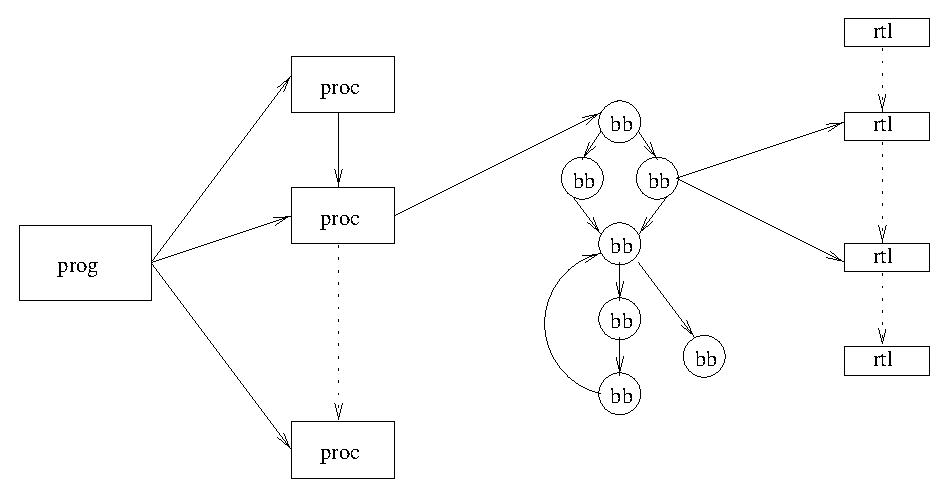
\includegraphics{figures/datastructs.eps}}
\centerfigend{fig-datastructs}{Data Structures to Represent a Binary Program}

We describe each of these parts of the intermediate representation
in reverse order, that is, starting from atomic data structures
and ending up with the program structure.



\section{Register Transfer Lists}
\label{sec-rtl}

{\small
\begin{flushright}
Design: Cristina, Mike; Documentation: Cristina, Doug, Mike;
 Implementation: Doug, David, Mike
\end{flushright} 
}

UQBT uses a simple, low-level register-transfer representation for the
effects of machine instructions.
A single instruction corresponds to a register-transfer list or RTL,
which in UQBT is a sequential composition of effects.
Each effect assigns an expression to a location.
All side effects are explicit at the top level;
expressions are evaluated without side effects, using purely
functional \emph{RTL operators}.
For example, the effects of the SPARC \texttt{call} instruction are
represented by the following RTL:

\begin{smallverbatim}
r[15] := %pc
%pc   := %npc
%npc  := r[15] + (4 * disp30)
\end{smallverbatim}
This sequence of effect puts the program counter~\texttt{\%pc} in
register~15, copies the ``next program counter''~\texttt{\%npc} into
the program counter, and puts the target address into~\texttt{\%npc}.
Because the target address is computed relative to the \emph{original}
program counter, the target-address computation uses register~15,
which holds the original value of~\texttt{\%pc}.
Because the SPARC uses delayed branches,  the target address
is placed into \texttt{\%npc}, not directly into \texttt{\%pc}.

Register transfer lists (RTLs) capture the semantic information 
of machine instructions by means of a series of \emph{effects} on a 
\emph{location}.
One register transfer is an assignment of an expression (i.e. an 
effect) to a location (i.e. a register or memory).  
There are no side effects, all effects are explicitly mentioned in 
the RTL.
The RTL environment assumes an infinite number of registers and
infinite memory space.  Memory is a sequence of bytes.  
{\it We will need specialized types of memory, such as memory for 
local variables, once the analysis has been formalized.   We
will do that then, so for now, there is only one type of memory. }

An `RTL language' is defined by a collection of locations and
operators.
UQBT uses an RTL language defined by taking the union of locations on
machines M$_S$ and M$_T$ and the union of the operators used in the
descriptions of machine M$_S$ and M$_T$.
The `machine~$X$ invariant' defines a sub-language of RTLs called
the $X$-RTLs; an RTL is an $X$-RTL if and only if it can be represented
as a single instruction on machine~$X$.

\uqbt 's \rtl\ implements the semantic information expressed in SSL
notation (SSL is described in Chapter~\ref{ch-ssl}).  

\subsection{Types}
\label{sec-rtltypes}
We define the following types to work with RTLs.  
(NOTE that these names should be in uppercase and perhaps shorter.
I've listed them as they appear in the rtl.h interface so that we don't
get confused -- when those are updated, these should be updated).
\begin{description}
\item[RTlist] a list of register transfers. Various analysis
    functions work on RTlists, such as GetControlTransfer().

\item[RTLInstDict] a dictionary of expanded instructions from the SSL
    file.

\item[RT] a register transfer is an assignment statement
    which has a variable (i.e. location) as the left-hand
    side and an expression (i.e. value) on the right-hand side. \\
    {\it We have considered introducing in the future a specialized
    RT which is a call, but at present that has not been decided
    upon.  We think it will be useful for analysis purposes. }

\item[RTAssgn] a subclass of class RT, representing an RT assignment
    (i.e. location := expression). One instruction may have zero
    (for NOP only) or more of these.

\item[RTFlagDef] a subclass of class RT, representing the definition
     of a flag function.

\item[RTFlagCall] a subclass of class RT, representing the call to a
    flag function.

\item[SemStr] a Semantic String, which is a prefix linearisation of an
    expression tree (see below).
    A SemStr can be used to represent a location, value, or subexpression.

    Expression operators are reproduced in Figure~\ref{fig-expOps2}.

% I'm not sure what this was meant to be about... probably some restriction
% on expressions which has long faded from the code. I keep it in comments
% in case it's not what I think it is. MVE
\begin{comment}
    {\it This may need to go elsewhere - Mike}
    An address expression is constrained to plus or minus offsets 
    from an address, hence the case \texttt{M[reg + reg * kte]} is not 
    supported directly; a subexpression needs to be computed into a 
    register and used as a register index in this case.

    These 3 options can be represented by 2: registers or constants.
    When an address expression is received, it is computed into 
    a register and that register is used to index into memory. 
    In this way we do not constrain address expressions (given that
    other machines may have more complicated addressing modes) 
    and create a simpler interface.
\end{comment}

\end{description}

\centerfigbegin
\begin{tabular}{|l|l|c|c|c|l|l|} \hline
Type of Operator & Id       &
\multicolumn{3}{c|}{Arguments}
& Symbol    & Meaning \\ \cline{3-5}
    &   & Int & Fix & Var & & \\
\hline
unary       & idNot         &0&0&1  & \verb!~!  & logical not \\
            & idNeg         &0&0&1  & 0-        & unary minus \\
\hline
binary      & idPlus        &0&0&2  & +         & addition \\
            & idMinus       &0&0&2  & -         & subtraction \\
            & idMult        &0&0&2  & *         & multiplication (unsigned)\\
            & idMults       &0&0&2  & *!        & multiplication (unsigned)\\
            & idDiv         &0&0&2  & /         & division (signed) \\
            & idDivs        &0&0&2  & /!        & division (signed) \\
            & idMod         &0&0&2  & \%        & modulus (unsigned) \\ 
            & idMods        &0&0&2  & \%!       & modulus (signed) \\ 
            & idBitAnd      &0&0&2  & \&        & (bitwise) and \\
%           & idBitAndNot   &0&0&2  & \&\~      & (bitwise) and-not \\
            & idBitOr       &0&0&2  & $|$       & (bitwise) or \\
%           & idOrNot       &0&0&2  & $|$\~     & (bitwise) or-not \\
            & idBitXor      &0&0&2  & \verb!^!  & xor \\
%           & idBitXorNot   &0&0&2  & \verb!^~! & xor-not \\
            & idShiftR      &0&0&2  & $>>$      & right-shift \\
            & idShiftL      &0&0&2  & $<<$      & left-shift \\
            & idShiftRA     &0&0&2  & $>>$A     & right-shift-arithmetic \\
            & idRotateL     &0&0&2  & rl        & rotate-left \\
            & idRotateR     &0&0&2  & rr        & rotate-right \\
            & idRotateLC    &0&0&2  & rlc       & rotate-left-through-carry \\
            & idRotateRC    &0&0&2  & rrc       & rotate-right-through-carry \\
\hline
ternary     & idTern        &0&0&3  & ?:        & c-style ternary \\
            & idAt          &0&0&3  & @         & bit extraction \\
\hline
logical     & idEquals      &0&0&2  & =         & equal \\
            & idNotEqual    &0&0&2  & \verb!~=! & not equal \\
            & idLess        &0&0&2  & $<$       & less than, signed \\
            & idGreater     &0&0&2  & $>$       & greater than, signed \\
            & idLessEq      &0&0&2  & $<=$      & less or equal to, signed \\
            & idGreaterEq   &0&0&2  & $>=$      & greater or equal to, signed \\
            & idLessUns     &0&0&2  & $<$u      & less than, unsigned \\
            & idGtrUns      &0&0&2  & $>$u      & greater than, unsigned \\
            & idLessEqUns   &0&0&2  & $<=$u     & less or equal to, unsigned \\
            & idGtrEqUns    &0&0&2  & $>=$u     & greater or equals, unsigned \\
            & idAnd         &0&0&2  & and       & and (of two expressions) \\
            & idOr          &0&0&2  & or        & or \\
\hline
operations  & idMemOf       &0&0&1  & m[...]    & memory of \\
            & idRegOf       &0&0&1  & r[...]    & register of \\
            & idAddrOf      &0&0&1  & a[...]    & address of (cancels m[]) \\
            & idVar         &1&0&0  & v\it{n}   & variable; replaces reg or mem \\
            & idParam       &0&1&0  & param`...'& parameter \\
            & idRparam      &0&1&0  & rparam`...'& register parameter \\
            & idExpand      &0&1&0  & expand`...'& expand (not for user) \\
            & idTemp        &0&1&0  & temp`...' & temporary register \\
            & idSize        &1&0&1  & size \it{n}& size cast \\
            & idDef         &0&1&0  & def `...' & definition; special for UQDBT \\
            & idIndex       &0&0&2  & [...]     & special for UQDBT \\
\hline
constants   & idIntConst    &1&0&0  & int \it{n}& integer constant \\
            & idFloatConst  &2&0&0  & float \it{f}& floating point constant \\
\hline
\end{tabular}
\centerfigend{fig-expOps2}{Expression Operators for RTL (cont over page)}

\centerfigbegin
\begin{tabular}{|l|l|c|c|c|l|l|} \hline
Type of Operator & Id       &
\multicolumn{3}{c|}{Arguments}
& Symbol    & Meaning \\ \cline{3-5}
    &   & Int & Fix & Var & & \\
\hline
type conversions& idSignExt &0&0&1  & !         & sign-extend (no sizes) \\
            & idTrunc       &2&0&1  & trunc(\it{exp, s1, s2})& truncate from s1 to s2 bits \\
            & idZfill       &2&0&1  & zfill(\it{exp, s1, s2})& zero fill from s1 to s2 bits \\
            & idSgnEx       &2&0&1  & sgnex(\it{exp, s1, s2})& sign extend from s1 to s2 bits \\
\hline
float conversions&idFsize   &2&0&1  & fsize(\it{exp, s1, s2})& float size convert from s1 to s2 \\
            & idItof        &2&0&1  & itof(\it{exp, s1, s2})& integer to float, s1 to s2 bits \\
            & idFtoi        &2&0&1  & ftoi(\it{exp, s1, s2})& float to integer, s1 to s2 bits \\
            & idFround      &2&0&1  & fround(\it{exp, s1, s2})& float round, s1 to s2 bits \\
\hline
\end{tabular}
\centerfigend{fig-expOps2a}{Expression Operators for RTL (cont from prev page)}

\subsection{Interface Functions to Create and Use RTLs}
All objects have constructor and destructor functions, as well
as functions to access elements of an object.  
Specialized analysis-related functions are explained in the
last subsection of this section---Functions for Analysis 
Purposes.  \\
{\it This style file doesn't number subsub sections,
how annoying! }


\subsubsection{Semantic String Class}
A semantic string object (SemStr) is a prefix linearisation of a tree
of RT components, such as constants, registers, memory, and various
expressions involving these. It is inplemented as a list of integers
(called items);
many of these integers are indices into a special table called the
Semantic Table. Entries in this table represent various things, such
as operators, special registers, parameters, and so on.

Here are a few examples: index 0 (the first entry) is called \texttt{idPlus},
and represents binary addition. Approximately index 75 is called
\texttt{idIntConst}, representing an integer (the actual integer is the next
integer in the string, following the {\tt idIntConst}).  So the expression
\texttt{2+2} is represented by the string ``{\tt 0 75 2 75 2}'' (read this
as ``plus int 2 int 2''). 

All the operators listed in Figure~\ref{fig-expOps2} are automatically
included in the table, and they are
machine independent. Special registers (e.g. the Next Program Counter register
({\tt \%npc}) and parameters (e.g. {\tt rs1} for the first source
register) are added
by the parser of the SSL file (see Chapter~\ref{ch-ssl}).
Let's consider a complete RTAssgn, conventionally written as

{\tt r[4] = m[1000] + 5}

This will be implemented as two semantic strings, one for the
location (left hand side) and one for the value (right hand side).
Each will be a list of integers, which might be

{\tt 34 75 4} ~~~and~~~ {\tt 0 38 75 1000 75 5}

and might print as

{\tt r[4]} ~~~and~~~   {\tt m[1000] + 5}  ~~~normally (the "int" is dropped
for brevity), or

{\tt r[ int 4]}  ~~~and~~~  {\tt + m[ int 1000 ] int 5}

if you choose to use the printPrefix() member function. This latter
representation is better for debugging problems with semantic strings,
though obviously it is less readable.

The first SemStr could be read as ``RegOf int 4''. The first integer, 34,
is an index into the semantic table, where among other information
there is the string ``r['' (for the SemStr print routine).
The enumerated constant ``idRegOf'' can be used in programs to
represent this index (see Figure~\ref{fig-expOps2} for a complete list
of these enumerated constants). The second integer,
75, is also an index into the semantic table, and says that the integer
following this index is to be taken as a literal integer. The third
integer, 4, represents itself. The second semantic string is a little
more complex. Its first index, 0, represents addition. The two arguments
to be added come next, but they are variable length. Immediately after
the 0 is 38, representing "memory of". The thing following the MemOf
could be any kind of expression; in this case it's ``int 1000'', but
it could have been say ``{\tt+ 500 500}'', or ``{\tt - r[ int 16 int 8}''.

Note that special registers (such as {\tt \%pc} or {\tt \%CF}) are
represented differently from general purpose registers. General purpose
registers are numbered, whereas special registers have their own
index into the semantic table (see Section~\ref{sec-semtable}).

A word on nomenclature: the word {\it parameter} is used to describe
a part of an instruction that will be {\it instantiated} with the
RTL function. For example, ``regorimm'' could be a parameter representing
a part of an instruction; actual values could be ``r[4]'' or ``4''.
The word {\it argument} is used here to mean those parts of a semantic
string that represent arguments (or operands) to the first index. For example,
if the first index is {\tt idMinus}, then there are two variable length
arguments to it, representing the minuend and the subtrahend respectively.
If the first index is idSize, there is one integer argument (the number
of bits in the size being cast to), and one variable length argument
(the expression being size cast).

Every semantic string has a type (e.g. unsigned integer 32 bits); the type is
represented by class Type (see Section~\ref{sec-class-type}). If not explicitly
specified, the semantic string is assigned the default type (which is signed
integer 32 bits). This type is preserved when semantic strings are copied,
subexpressions are made, and so on.

\begin{itemize}
\item   SemStr: $\emptyset$ \ra SemStr.
    Default constructor.

\item   SemStr: Kind \ra SemStr.
    Constructor that takes an expression kind. The kinds are only these:
    uORDINARY, eOPTABLE, and eCONDTABLE. Not for users.

\item   SemStr: SemStr \ra SemStr.
    Copy constructor.

\item   operator=: SemStr \ra SemStr.
    Assignment operator.

\item   SemStr: (Iterator1 x Iterator2) \ra SemStr.
    Constructor that takes a pair of iterators. Makes a copy of part
    of some other SemStr starting with the item referenced by iterator1
    up to but not including iterator2.

\item   SemStr: (int* x int* x Kind) \ra SemStr.
    Constructor that takes two pointers to an array of integers (pointer to
    first and pointer to last). Also takes kind, as above.

\item   getKind: SemStr \ra Kind.
    Gets the kind as above. Not for users.

\item   getType: SemStr \ra Type.
    Gets the type (as class Type) for the semantic string.

\item   isFloat: SemStr \ra BOOL.
    Note: deprecated. Returns true if the expression this semantic string
    represents is a floating point type.

\item   setType: (SemStr x Type) \ra $\emptyset$.
    Set the type for the expression that this semantic string represents.

\item   setTypes: (SemStr x SemStr) \ra $\emptyset$.
    Set the type for this semantic string to be the same as the type of the
    given semantic string.

\item   operator==: (SemStr x SemStr) \ra BOOL.
    Returns true if this SemStr is equal to the given SemStr. Type is taken
    into account in the comparison.

\item   operator\%=: (SemStr x SemStr) \ra BOOL.
    Same as above, except that type is \emph{not} taken into account.

\item   operator-=: (SemStr x SemStr) \ra BOOL.
    Same as the two above, except that only the sign element of the type is
    disregarded. Therefore, to return true, the expressions must match, and
    the size and broad type must match, but the ``signedness'' need not
    match.

\item   operator$<$: (SemStr x SemStr) \ra BOOL.
    Returns true if this SemStr is ``less than'' the given SemStr. Comparison
    is arbitrary, but establises a unique ordering of semantic strings. This
    function is often used implictly where there are maps of semantic strings.
    Type is included in the comparison.

\item   operator$<<$: (SemStr x SemStr) \ra BOOL
    Same as the above, except that ``signedness'' is not considered in the
    comparison.

\item   push: (SemStr x int) \ra $\emptyset$.
    Push the given integer to the end of the semantic string. It is up to
    the user to make sure that the semantic string is valid.

\item   prep: (SemStr x int) \ra $\emptyset$.
    Prepend the given integer to the front of the semantic string. It is
    up to the user to make sure that the semantic string is valid.

\item   pushSS: (SemStr x SemStr) \ra $\emptyset$.
    Push a copy of the given semantic string to the end of this string

\item   pushArr: (SemStr x int x int*) \ra $\emptyset$.
    Push the given number of integers from the given array of integers to
    the end of the string.

\item   pop: $\emptyset$ \ra int.
    Remove the last integer from the list, and return it.

\item   popFirst: $\emptyset$ \ra int.
    Remove the first integer from the list, and return it.

\item   clear: $\emptyset$ \ra $\emptyset$.
    Set this semantic string to be empty (no elements in the list).

\item   isSpRegEqual: (SemStr x int) \ra BOOL.
    Returns true if this semantic string matches the special register
    whose index is given. Not for most users.

\item   isSpRegCont: (SemStr x int) \ra BOOL.
    Returns true if this semantic string contains the special register
    whose index is given. Not for most users.

\item   isNumRegEqual: (SemStr x int) \ra BOOL.
    Returns true if this semantic string matches the register
    whose number is given. Not for most users.

\item   isNumRegCont: (SemStr x int) \ra BOOL.
    Returns true if this semantic string contains the register
    whose number is given. Not for most users.

\item   isArrayEqual: (SemStr x Array of int) \ra BOOL.
    Returns true if the elements of this semantic string match the
    elements of the given array of integers. Can be used to test for
    specific semantic strings, e.g. ``\%pc = \%npc''.

\item   getFirstIdx: SemStr \ra int.
    Returns the first item of this semantic string. Note that this really
    should be called getFirstItem, since the integer returned may not actually
    be an index (it could be an integer constant, or even half of a floating
    point constant).

\item   getSecondIdx: SemStr \ra int.
    Returns the second item of this semantic string. Usually used where
    the first index is known to contain one integer or fixed argument
    (e.g. the first index is idIntConst or idSize).

\item   getThirdIdx: SemStr \ra int.
    Returns the third item of this semantic string.

\item   getSubExpr: (SemStr x int) \ra SemStr*.
    Returns a pointer to a new semantic string, which is composed of
    the given subexpression. Passing zero returns the first argument
    to this expression, one returns the second, and so on.
    {\bf Note:} This member function only works with variable arguments.
    Use GetSecondIdx to access an integer or fixed argument.

\item   getSubExpr: (SemStr x int x SemStr) \ra SemStr.
    As above, but also stores the result in the reference (last) parameter.
    This ensures that the caller will automatically delete the semantic string
    when it goes out of scope.

\item   getIndex: (SemStr x int) \ra int.
    Get the {\it i}th item (where {\it i} is given).

\item   getLastIndex: SemStr \ra int.
    Get the last item of the list of integers in this semantic string.

    The next group of member functions concern searching for a subexpression
    withing this semantic string. An item of -1 in a semantic string is treated
    as a ``wildcard''.
    Formally, a search expression (S) will match a subexpression (E) if:

    length(S) $<=$ length(E) and for each position, p, in S the following holds:

    S[p] == -1 $||$ S[p] == E[p]

    Example: if {\it this} is \{0,\{3,78\},\{43,6,14\}\},
    it can be searched with the following subexpressions, and will return true:

\begin{tabular}{|l|l|} \hline
    Search & Result \\
\hline
    \{\{3,78\}\} & \{\{3,78\}\} \\
    \{\{0,*,*,\{43\}\}\} & \tt\{\{0,\{3,78\},\{43,6,14\}\}\} \\
\hline
\end{tabular}

\item   search: (SemStr x SemStr x SemStr x BOOL) \ra BOOL.
    Searches this semantic string for the given subexpression (first parameter
    after {\it this}). If found, the matching string is copied to the reference
    (last SemStr) parameter. The return value is whether a match was found.
    If the optional boolean is set, the search is type
    sensitive (i.e. the types have to match, as well as the expressions). This
    boolean defaults to false (i.e. the search defaults to case insensitive).

\item   searchAll: (SemStr x SemStr x list\{SemStr*\} x BOOL) \ra BOOL.
    Searches this semantic string for {\it all} occurrences of the given
    subexpression (first parameter after {\it this}). For each match, the
    matching string is appended to the list of pointers to semantic strings.
    The return value is whether any match was found.
    If the optional boolean is set, the search is type
    sensitive (i.e. the types have to match, as well as the expressions). This
    boolean defaults to false (i.e. the search defaults to case insensitive).

\item   searchReplace: (SemStr x SemStr x SemStr x BOOL) \ra BOOL.
    Searches this semantic string for the given subexpression (first parameter
    after {\it this}). If found, the matching string is replaced by the
    reference (last SemStr) parameter. The return value is whether a match was
    found.
    If the optional boolean is set, the search is type
    sensitive (i.e. the types have to match, as well as the expressions). This
    boolean defaults to false (i.e. the search defaults to case insensitive).

\item   searchReplaceAll: (SemStr x SemStr x SemStr x BOOL) \ra BOOL.
    Searches this semantic string for {\it all} occurrences of the given
    subexpression (first parameter after {\it this}). For each match, the
    matching string is replaced by the given string (last SemStr parameter).
    The return value is whether any replacement was made.
    If the optional boolean is set, the search is type
    sensitive (i.e. the types have to match, as well as the expressions). This
    boolean defaults to false (i.e. the search defaults to case insensitive).

\item   substReg: (SemStr x int x SemStr) \ra BOOL.
    Substitute all occurrences of the given numbered register with the given
    semantic string. Returns true if any match found.
 
\item   substSpcl: (SemStr x int x SemStr) \ra BOOL.
    Substitute all occurrences of the given special register (index is given)
    with the given semantic string.

\item   substIndex: (SemStr x int x int) \ra $\emptyset$
    Replace the item at the given index with the given integer. For example,
    substIndex(0, 77) will replace the first item in the list with 77.
 
\item   smartCompare: (SemStr x SemStr x BOOL x list\{int\}) \ra BOOL.
    This function is not complete. Do not use.

\item   findEndSubExpr(SemStr x iterator) \ra iterator.
    Given an iterator into this semantic string, step forward towards the end
    of this string until the end of the subexpression headed by the given
    iterator is found. Returns an iterator that is just past the end of that
    subexpression. For example, if given (3+4)*(5+6) (internally
    * + int 3 int 4 + int 5 int 6), with an iterator pointing to the first
    plus, returns an iterator to the second plus (just past the (3+4)
    subexpression).
    There are actually two functions with the same name; one takes and
    returns a const iterator, and one takes and returns a non-const iterator.

\item   simplify: SemStr \ra $\emptyset$
    Simplify this expression using constant folding and the like, and also
    cannonicalising the expression by placing integer constants on the
    right if possible (so 2+a is replaced by a+2). a + -2 is replaced by a-2.
    a $<<$ k is changed to a * K where K=2**k.

\item   findSubExpr: (SemStr x int x int* x int) \ra BOOL.
    Search this semantic string for the expression (given by the given number
    of integers in the given array of integers). Returns true if found. If
    found and there were wildcards in the array, the item matched by the last
    wildcard is written to the reference (last) parameter.

\item   sprint: SemStr \ra string.
    Prints a representation of this semantic string to a string, which
    is returned. This is a conventional (infix) representation, and
    so it somewhat removed from the actual (prefix) implementation.
    Some effort is made to pretty the result, e.g. r[ int 4] is
    displayed as r[4].
    When exact knowledge of the format of the string is required, use
    sprintPrefix below.

\item   print: (SemStr x ostream) \ra $\emptyset$.
    Prints a representation of the semantic string to the given stream,
    or to cout if none is given. It is equivalent to printing the string
    returned by sprint to the given stream.

\item   sprintPrefix: SemStr \ra string.
    Prints a representation of this semantic string to a string, which
    is returned. The format is strongly tied to the internal (prefix)
    representation of the semantic string, so it is harder to read than
    the result from sprint, but may be more useful for debugging.

\item   printPrefix: (SemStr x ostream) \ra $\emptyset$.
    Prints a representation of the semantic string to the given stream,
    or to cout if none is given. It is equivalent to printing the string
    returned by sprintPrefix to the given stream.

\item   len: SemStr \ra int.
    Returns the number of items in this semantic string.

\item   instantiate: (SemStr x list\{int\} x vector\{char*\} x RMAP) \ra BOOL.
    Replace all occurrences of formal instruction parameters (e.g. rs1) with
    actual expressions (e.g. r[12]). The last parameter is an object
    representing the register map. Not for users.

\end {itemize}

\subsubsection{Semantic Table Class}
\label{sec-semtable}

Semantic Strings (class SemStr) are mainly indices into a special
object of class SemTable, the semantic table. This is a global
object, accessable as {\tt theSemTable} as long as you
{\tt \#include "ss.h"}. Most of the time, the user need not be
concerned with the semantic table, but there are a few important
exceptions.

One of these is when dealing with special registers. These registers
are not accessed like general purpose registers (so called {\it numbered}
registers), but have their own entries in the semantic table. When
special registers are referenced in the SSL file (see Chapter~\ref{ch-ssl}),
they are placed into
the semantic table by the parser. The index of a particular special
register is not fixed (most of them are machine specific), so there is no
enumerated constant like {\tt idPlus} that can be used for a special
register. At present, the way to find an appropriate index is to use
the FindRegIndex member function.

\begin{itemize}
\item   findRegIndex: (SemTable x string) \ra int.
    Given the semantic table and a string representing the name of the
    special register (including the {\tt \%}), returns an integer index
    for the appropriate semantic table item. This single index
    represents the special register in semantic strings (compared with
    three integers for a numbered register).

\item   findOpIndex: (SemTable x char*) \ra int.
    Given a C string representing the operator (e.g. {\tt \verb!"&~"!}),
    returns the index representing the operator. This operator can be
    used to build expressions, etc. Note that this function is not
    efficient (at present, it uses a linear search), so it should not
    be used where the operator is known (in this case, {\tt idBitAndNot});
    use it where the operator could be one of a number of values, and
    only the string representation is known. (For example, the SSL
    parser uses this function when parsing SSL expressions).

\end{itemize}

\subsubsection{Type Class}
\label{sec-class-type}
Types inside Semantic Strings and elsewhere are represented by class Type.
A Type has three components: the broad type, sign, and size. The broad type
is given in terms of this enumerated type:

\begin{verbatim}
enum LOC_TYPE {
    VOID = 0,               // void (for return type only)
    INTEGER,                // integer (any size and signedness)
    FLOAT,                  // a floating point (any size)
    DATA_ADDRESS,           // a pointer to some data (e.g. char*, struct*,
                            // float* etc)
    FUNC_ADDRESS,           // a pointer to a function
    VARARGS,                // variable arguments from here on, i.e. "..."
    UNKNOWN
};
\end{verbatim}

A particular type is given by either a tuple (e.g. (INTEGER, unsigned, 32 bits))
or a couple (e.g. (FLOAT, 64 bits); the sign is irrelevant for a float, but
defaults to signed).

\begin{itemize}
\item   Type: $\emptyset$ \ra Type.
    Default constructor. Returns the default type, which is 32 bit signed
    integer.

\item   Type: (LOC\_TYPE x int x BOOL) \ra Type.
    Constructor, with type given as a LOC\_TYPE (see abvove), size in bits,
    and if the LOC\_TYPE is integer, a BOOL for sign (TRUE = signed).

\item   operator==: (Type x Type) \ra BOOL.
    Equality operator. Sign is considered in the comparison, so the types must
    match in all respects for this function to return TRUE.

\item   operator-=: (Type x Type) \ra BOOL.
    Equality operator. Sign is {\it not} considered, so for this function to
    return true, the broad types and size must match, but the sign need not.

\item   operator$<$: (Type x Type) \ra BOOL.
    Less than operator. Sign is considered in the comparison.
    This function establishes an arbitrary ordering among all types.

\item   operator$<<$: (Type x Type) \ra BOOL.
    Less than operator. Sign is {\it not} considered in the comparison.
    This function establishes an arbitrary ordering among all types.

\item   getSize: Type \ra int.
    Returns the size (in bits) component of the Type.

\item   getType: Type \ra LOC\_TYPE.
    Returns the Type component of the Type, as a LOC\_TYPE.

\item   getSize: Type \ra BOOL.
    Returns the sign component of the Type; TRUE if signed.

\item   setSize: (Type x int) \ra $\emptyset$.
    Sets the size (in bits) component of this Type.

\item   setType: (Type x LOC\_TYPE) \ra $\emptyset$.
    Sets the Type component of this Type, given a LOC\_TYPE.

\item   setSize: (Type x BOOL) \ra $\emptyset$.
    Sets the sign component of this Type; TRUE if signed.

\item   getCtype: Type \ra CHAR*.
    Returns a C-style null terminated string representing the C language
    equivalent of the type. For example, if the type is (integer, unsigned, 16)
    the returned string would be ``unsigned short''.

\end{itemize}


\subsubsection{Register Transfer Assignment Class}
A register transfer assignment (RTAssgn) object is an assignment of an
expression
to a location.  A register transfer object also has size information
to determine the number of bits of information transferred from
the expression to the location.

\begin{itemize}
\item  updateLHS: (RTAssgn x Location) \ra RT.
    Given an RT object and a location, the location
    information gets updated in the object.

\item  updateRHS: (RTAssgn x Expr) \ra RT.
    Given an RT object and an expression, the expression
    information gets updated in the object.

\item  updateSize: (RTAssgn x BYTE) \ra RT.
    Given an RT object and a size in bits, the size of the
    transfer information gets updated in the object.

\item  getLHS: RTAssgn \ra SemStr*.
    Given an RTAssgn object, returns a pointer to the semantic string
    representing the location of the assignment.

\item  getRHS: RTAssgn \ra SemStr*.
    Given an RTAssgn object, returns a pointer to the semantic string
    representing the expression of the assignment.

\item  getSize: RTAssgn \ra BYTE.
    Given an RT object, returns the size in bits of the transfer
    of information.
\end{itemize}


\subsubsection{Register Transfer List Object}
A register transfer list (RTlist) is a list of register transfer 
objects.  However, greater functionality is provided for this 
object for analysis purposes; those functions are described in the 
next section.
For traversal purposes, an RTlist keeps track of the `current'
register transfer being traversed (by default, the first one
in the list).

\begin{itemize}
\item RTlist: $\emptyset$ \ra RTlist.
    Constructor function which returns an empty object of type RTlist.

\item RTlist: (RTlist x RTlist) \ra RTlist.
    Copy constructor: given a source and destination RTlist 
    objects, copies the first one onto the second one.

\item insertRT: (RTlist x RT) \ra RTlist.
    Given an RTlist object and a register transfer, inserts the
    register transfer at the end of the list.

\item updateRT: (RTlist x RT x int) \ra RTlist.
    Given an RTlist object, a register transfer and an index position into
    a list, updates the indexed register transfer in the list
    with the new one (if possible), otherwise it does not modify
    the RTlist object.
\end{itemize}


\subsubsection{Functions for Analysis Purposes}
The following functions are required for analysis purposes and
are described per relevant object.
More functions will be added as we see fit.


\paragraph{Register Transfer Assignment Class}
Functions that allow users to know which registers are defined
and used in the register transfer.  Note that this information
is implicitly stored in the LHS and RHS fields of an 
RTAssgn object.

\begin{itemize}
\item  isSpRegDefined: (RTAssgn x int) \ra BOOL.
    Given a register transfer assignment object and an index representing
    a special register, returns 
    whether the register is defined in the assignment or not.

\item  isNumRegDefined: (RTAssgn x int) \ra BOOL.
    Given a register transfer assignment object and the number of a
    numbered register, returns whether that register was defined
    in the register transfer or not.

\item  isSpRegUsed: (RTAssgn x int) \ra BOOL.
    Given a register transfer assignment object and an index representing
    a special register, returns whether
    that register was used by the object or not.

\item  isNumRegUsed: (RTAssgn x int) \ra BOOL.
    Similar to IsRegUsed() but for a numbered register.

\item  numRegUse: RTAssgn \ra int.
    Given a register transfer object, returns the number of registers
    used by that transfer. \\
    {\it Not implemented at present. A similar function that returns a list of registers used may
    be useful. }

\item  numRegDef: RTAssgn \ra int.
    Given a register transfer object, returns the number of registers
    that were defined by that transfer. \\
    {\it Not implemented at present. A similar function that returns a list of registers defined may
    be useful. }
\end{itemize}


\paragraph{Register Transfer List Object} 
The RTlist object \emph{will} provide in the \emph{future} 
functions that allow us to quickly decide what type of 
instructions we are dealing with.  The following are two
such functions which are not currently implemented:

\begin{itemize}
\item RTL: (STRING x ADDRESS x ...) \ra RTlist.
    This function returns an instance of a register transfer
    list for a particular machine instruction.  The name
    of the instruction is a named used in the SSL specification,
    these names are normally the same names used in SLED
    specifications.   The given native address is the program counter's
    address and is stored for usage when building a control
    flow graph of the procedure (see Section~\ref{sec-cfg}). \\ 
    The function returns an instance of an RTlist by reading
    the template file generated by SRD (refer to Section~\ref{sec-srd},
    Chapter~\ref{ch-ssl}).  \\

\item getBBSuccAddr: (RTlist x int) \ra ADDRESS.
    Given an RTlist object and an index position, returns the 
    address associated with that out-edge (if any) or Nil 
    otherwise.  \\
    This function is useful to construct a control flow graph,
    see example in Section~\ref{sec-cfg-eg}. 

\item getBBProcAddr: RTlist \ra ADDRESS.
    Given a call register transfer list, returns the target procedure 
    call address (if any) or Nil otherwise. \\
    This function is useful to construct a control flow graph,
    see example in Section~\ref{sec-cfg-eg}.

\item getNumRT: RTlist \ra int.
    Given an RTlist, returns the number of elements (RTs) in
    the list.

\item getRT: (RTlist x int) \ra RT.
    Given an RTlist object and an index into the list, returns
    the corresponding register transfer (if it exists) or 
    Nil.
    Elements in a list are indexed from one.

\item nextRT: RTlist \ra RT.
    Given an RTlist object, returns the next RT in the list (if any)
    or Nil (if at the end of the list).  The `current' index is
    updated to point to the next element in the list. 

\item isControlTransfer: RTlist \ra CTTYPE.
    Given an RTlist object, checks if the set of register 
    transfers are equivalent to a control transfer instruction,
    if so, returns the type of control transfer instruction 
    (one of ONEWAY, TWOWAY, NWAY, CALL, or FALL), otherwise
    returns NONE.  
    A control transfer instruction is one that explicitly 
    modifies the value of the program counter register.
\end{itemize}



\subsection{Usage of this Interface}
\label{sec-usageRTL}
A user can integrate RTL into a NJMC matching statement in
the following way: once an instruction has been decoded 
by matching one of the arms of the \texttt{match} statement, 
an instance of the matched instruction can be obtained in 
RTL form by passing the (unique) name of the instruction to
the RTL dictionary, along with the values of the other parts
of the instruction.  The RTL system will return an instance
of an entry in the dictionary. 
At present, the RTL instance function expects to receive 
the native address of the instruction being decoded, its name 
(i.e. key), and its arguments in string form.  The native 
address is required later on, for the purposes of constructing
a control flow graph of the program (see Section~\ref{sec-cfg}).

The following sample code illustrates the usage of this interface
with a SPARC matching statement.
The function \texttt{decode\_instr} implements a matching statement
which decodes the machine instruction pointed to by the \texttt{pc}
variable.  If the \texttt{alu} arm is matched, the \texttt{name} 
variable will hold the name of the arithmetic-logical instruction
matched.  The \texttt{RTLDisc.RTL} function is called with the
string values for the other parts of the arithmetic-logical 
instruction: the first register operand (\texttt{rs1}), the 
second register or immediate operand (matched in the \texttt{dis\_roi}
function), and the destination register \texttt{rd}).  Macros
are used (\texttt{RS1}, \texttt{ROI} and \texttt{RD}) to make
the translation from integer to strings depending on the context.
In the case of branch and call instructions, the target address passed
to the RTL dictionary is the \emph{raw} offset address given in the
instruction, rather than the relocated one; hence the need for the
equation provided to restore this value.  Alternatively, the 
core SLED spec for SPARC could be modified so that it does not 
relocate addresses automatically---this has not been done at 
present for consistency with disassemblers.

{\small
\begin{verbatim}
#define RD   (rd_names[rd])
#define RS1  (rs1_names[rs1])
#define RS2  (rs2_names[rs2])
#define ROI  (dis_roi(roi))

char *dis_roi(ADDRESS lc) {
  static char buf[512];
  match lc to
  | imode(i)   => sprintf(buf, "%d", i); return buf;
  | rmode(rs2) => return RS2;
  endmatch
}

void decode_instr (ADDRESS pc, ADDRESS uNativeAddr, RTLInstDict RTLDict, RTlist &rtl)
{
    match pc to
    | ...
    | alu (rs1, roi, rd) [name] => 
            rtl = RTLDict.RTL (uNativeAddr, name, RS1, ROI, RD);
    | branch^a (tgt, a) [name] => 
            sprintf(anulled, "%d", a);      // 1 if anulled
            rtl = RTLDict.RTL (uNativeAddr, name, numToStr((tgt-pc)>>2), anulled);
    | call_ (tgt) [name] => 
            rtl = RTLDict.RTL (uNativeAddr, name, numToStr((tgt-pc)>>2)); 
    | ...
    endmatch
\end{verbatim}  
}

This type of code (the whole matching statement file) can
obviously be mostly generated automatically, but at this stage we
either generate a decoder usingthe NJMC toolkit and modify that
code, or write it manually.


\section{Control Flow Graphs}
\label{sec-cfg}

{\small
\begin{flushright}
Design: Cristina; Documentation: Cristina; Implementation: Mike, Cristina
\end{flushright} 
}

A control flow graph (CFG) is a directed graph that represents the flow of 
control of a program, thus, it only represents the flow of instructions 
(code) of the program and excludes data information.
The nodes of a CFG represent basic blocks of the program, and the edges 
represent the flow of control between nodes.  More formally,

\begin{definition} \cite{Aho86}
\label{def-bb}
A {\bf basic block} is a sequence of consecutive statements in which
flow of control enters at the beginning and leaves at the end without
halt or possibility of branching except at the end.   
\end{definition}


\begin{definition}
\label{def-cfg}
A {\bf control flow graph} $G = (N,E,h)$ for a program $P$ is a connected,
directed graph, that satisfies the following conditions:
\begin{itemize}
\item $h$ is the unique entry node to the graph, 
\item $\forall \, n \in N, n$ represents a basic blocks of $P$, and 
\item $\forall \, e = (n_{i},n_{j}) \in E, e$ represents flow of control from
basic block $n_{i}$ to basic block $n_{j}$, and $n_{i}, n_{j} \in N$.
\end{itemize}
\end{definition}


\subsection{Types of Basic Blocks}
For the purposes of CFG construction, basic blocks are
classified into different types, according to the {\em last} instruction in 
the basic block.  Given that the instructions in the basic block
represent a sequential list of instructions (that would be executed
in that order), machine dependencies on the flow of control such as 
SPARC's delayed instructions cannot appear in the graph; they need
to be abstracted away into a machine-independent form.

Ideally, only 6 types of basic blocks are available.  However, 
during static decoding of a binary executable, it is not always
possible to determine the target branches of indirect and indexed
transfers of control.  In these cases, we make use of a node called
{\em nowhere} as the node does not lead to anywhere.  This node
will be analysed at runtime.  
The basic block types are: 

\begin{description}
\item [one-way] the last instruction in the basic block is an
unconditional jump to a known target location, hence, the block has one 
out-edge.

\item [two-way] the last instruction is a conditional jump to a 
known target location, thus, the block has two out-edges.

\item [n-way] the last instruction is an indexed/indirect jump to
known target locations.  The $n$ branches located in the index table become 
the $n$ out-edges of this node.

\item [call] the last instruction is a call to a procedure.
There are two out-edges from this block: one to the instruction following
the procedure call, and the other to the procedure that is called.
Throughout analyses, the called procedure is normally not followed,
unless interprocedural analysis is required.

\item [return] the last instruction is a procedure return instruction.
There are no out-edges from this basic block.

\item [fall] the next instruction is the target address of a
branch instruction (i.e. the next instruction has a label).  This node
is seen as a node that {\it falls through} the next one, thus, there is
only one out-edge.

\item [nowhere] the last instruction is an indexed or indirect jump
or call to an unknown target location.  This node has no out-edges. 
\end{description}


\subsection{Abstractions}
Based on definitions~\ref{def-bb} and \ref{def-cfg}, we define two 
abstractions to work with control flow graphs.

\begin{description}
\item [BB] is a basic block.  A BB holds information about the
    RTL instructions that form part of that basic block, as 
    well as successors of the basic block.

\item [CFG] is a control flow graph.  A CFG is a reference to 
    the header of the graph, i.e. a BB, and stores extra information
    like the state of the graph (see next section).
    Extra functionality is provided for a CFG which is not 
    provided for a BB, as seen in Section~\ref{sec-ir-cfg}.
\end{description}


\subsection{Steps in Constructing a CFG}
Machine instructions that modify the flow of control of a program 
have two types of references to the target address: via a machine-dependent
(physical) address, or via an offset into the stream of machine
instructions for the program.  Offsets resolve to physical 
addresses too.   
There are three main steps in the construction of the CFG:
\begin{enumerate}
\item Create a machine-dependent CFG by building BBs of instructions
    that contain native addressess for transfers of control.
\item Transform the machine-dependent CFG into a machine-independent
    CFG by transforming address references into edges (references
    to basic blocks).
\item Optimize the machine-independent CFG to remove extraneous 
    basic blocks introduced by limitations in the machine 
    instruction set (e.g. a jump to a jump), hence reducing the 
    number of nodes and edges of the graph. 
\end{enumerate} 

We will refer to the machine-independent CFG as a {\em well-formed} CFG
or \wfCFG.  This graph is the one used for analysis purposes. 


\subsection{Interface Functions to Construct Basic Blocks}
\label{sec-ir-bb}
Basic blocks have limited functionality: they can be 
constructed, and machine-dependent (i.e. host address) out-edges 
can be added to them. 

\begin{itemize}
\item BasicBlock: $\emptyset$ \ra BB.
    Constructor for a basic block.

\item addOutEdge: (BB x ADDRESS) \ra BOOL.  
    Adds the address as an out-edge in the given basic block. 
    The mapping between addresses and basic blocks is done when 
    the graph is well-formed.
    Returns true if successful.

\item addInterProcOutEdge (BB x ADDRESS) \ra BOOL.
    Adds an interprocedural out-edge to the basic block pBB that
    represents this address.  The mapping between addresses and
    basic blocks is done when the graph is well-formed.
    Returns true if successful.

\item addProcOutEdge: (BB x ADDRESS) \ra BOOL.
    Given a CALL basic block and an address of a procedure (i.e. the
    target address of a call instruction), stores the information
    in the basic block. 
    \emph{This function is not yet implemented.}
\end{itemize}


\subsection{Interface Functions to Construct a CFG}
\label{sec-ir-cfg}
Control flow graphs are composed of machine-dependent basic block nodes 
initially, and can then be transformed to machine-independent nodes
which are used for analysis purposes.  This latter graph is referred
to as a well-formed graph. 
A doubly-linked graph (i.e one that has in- and out-edges) can only be 
built once the graph is well-formed.
Further, a well-formed graph can be optimized to remove redundant edges 
and nodes (e.g. jumps to jumps).
The following functionality is provided by the interface:

\begin{itemize}
\item Cfg: $\emptyset$ \ra Cfg.
    Constructor function for a CFG. The CFG is constructed empty, and
    has BBs added as required.

\item newBB: (CFG x RTL x RTL x BBTYPE x int x ADDRESS) \ra BB.  
    Allocates memory for a new basic block node, initializes it to 
    references to the first and last rtl's, its type, and allocates 
    enough space to hold the out-edges (the number of which is 
    given as a parameter).  
    The native address associated with the start of the BB is given;
    this address must be the same one used with AddOutEdge().
    A reference to the newly created basic block is returned.
    If there is not enough memory, an exception will be raised.
    \emph{Mike: what did we decide in the end for these cases?}

\item label: (CFG x ADDRESS) \ra BOOL.
    Checks whether the given native address is a label (explicit or 
    non-explicit) or not.  Explicit labels are addresses that have already 
    been tagged as being labels due to transfers of control to that 
    address.  Non explicit labels are those that belong to basic blocks 
    that have already been constructed (i.e. have previously been 
    parsed) and now need to be made explicit labels.  In the case of 
    non explicit labels, the basic block is split into two and types 
    and edges are adjusted accordingly.
    Returns true if the native address is that of an explicit or a non 
    explicit label, false otherwise. 

\item isLabel: (CFG x ADDRESS) \ra BOOL.
    Checks if the native address is a label or not in the current 
    control flow graph. 
    If not, the address is not added to the map of Lables to BBs.
    \emph{Mike: what does the last sentence mean?  i.e. every time
    an IsLabel() command is emmited, new labels are created??}

\item wellFormCFG: CFG \ra BOOL.  
    Transforms a machine-dependent CFG into a well-formed CFG (\wfCFG) 
    (i.e. a machine-independent one), by converting address references 
    of out-edges into references to basic blocks, and procedure
    address references into references to procedure structures 
    (the procedure structure is defined in Section~\ref{sec-ir-proc}).  
    Returns TRUE if successful.

\item isWellFormed: CFG \ra BOOL.
    Returns whether the graph is well-formed or not.

\item addInEdges: CFG \ra BOOL.  
    Given a \wfCFG, annotates each basic block with its in-edges 
    information.  Returns TRUE if successful.

\item compressCFG: CFG \ra BOOL.  
    Given a \wfCFG, optimizations are performed on the graph to reduce 
    the number of basic blocks and edges (if possible).  Returns
    TRUE if successful (whether or not the graph was compressed).
    The optimizations performed are: removal of branch
    chains (i.e. jumps to jump), removal of redundant jumps (i.e. jump
    to the next instruction), merge basic blocks where possible, and
    remove redundant basic blocks created by the previous optimizations.
\end{itemize}


\subsection{Interface Functions for Analysis Purposes}
Analysis functions are available to graphs of any kind; well-formed
or not.
In order to traverse a graph, a numbering scheme needs to be used
to uniquely identify the nodes in the graph in some fashion.  
For display purposes, the graph itself needs to be stored in a 
notation amenable for display, such as that provided by the Dotty 
interface. 

\begin{itemize}
\item numberCFG: CFG \ra BOOL.  
    Given a \wfCFG, each node in the graph is annotated with a unique 
    integer identifier.
    The method used at present is depth-first traversal, numbering
    nodes during the first visit to the node.
    We may change this numbering method later on.  
    Returns TRUE if successful.

\item writeDotFile: (CFG x STRING x int) \ra BOOL.  
    Given a \wfCFG\ and the name of an opened dotty (.dot) file,
    writes the information relating the control flow graph with
    node IDs offset by an integer value.  This property is used
    to give unique ID numbers to all nodes in a dotty file (a 
    requirement of the dotty interface).
    Returns TRUE if successful.
\end{itemize}


\subsection{Usage of this Interface}
\label{sec-cfg-eg}
A user may construct a control flow graph after having decoded  
the machine instructions and obtained their semantical 
RTL representation (see Section~\ref{sec-usageRTL}).  
Higher order instructions prevent us from creation of the graph 
at decoding time, due to the dependency of such instructions 
on an undecoded instruction.
\emph{However, note though that our current implementation 
creates basic blocks while decoding machine instructions; 
this gives us an approximation of the final graph but not 
a correct graph necessarily.  Analysis to remove higher order instructions
is missing at present, but is underway (in paper at least) -- cc,
27 May 98.}

The process of creating a \wfCFG\ is divided into two steps:
creating the basic blocks and creating the machine-independent
graph.  The former step can be done during the decoding of
machine instructions, as per the following code illustrates.
The function \texttt{followControl} drives the decoding of 
machine instructions by traversing paths in the program. 
While the code along one path has not been traversed, the 
function decodes one instructions (\texttt{decode\_instr}) and
checks if it is a control transfer instruction.  If so, based
on the type of the instruction, the type of the new basic
block is determined.  For example, if the parsed instruction
was an unconditional branch, then a one-way node is created,
with references to the first (\texttt{hdr}) and the last (\texttt{end})
rtls, and the target address of the jump. 
Once a node has been created, the target address is traversed 
recursively if it has not been traversed yet.  This is easily checked by 
determining if the target address is a label in the current 
graph or in another graph (as it may be an interprocedural branch).
The address for the next instruction to decode is determined, 
as well as the end of the section is checked.  The new target 
address is also checked for having been traversed---if it has, this
means that a fall-through node needs to be created rather than
decoding the same instructions twice.

{\small
\begin{verbatim}
// followControl()
// Precondition: the passed uNativeAddr is within the boundaries of
// the code section being decoded (i.e. uNativeAddr < upperNativeAddr).
// Precondition 2: the passed uNativeAddr is not an explicit label.
//
void followControl (ADDRESS uHostAddr, ADDRESS uNativeAddr,
                    ADDRESS upperNativeAddr, RTLInstDict RTLDict, LRTL &rtls,
                    Cfg &cfg)
{ BOOL done;
  INSTYPE type;
  RTL_CIT hdr, end;
  PBB pBB;

    while (! done)
    {
        // decode the inst at uNativeAddr (pointed to by uHostAddr)
        decode_instr (uHostAddr, uNativeAddr, buffer, RTLDict, rtl);

        // traverse paths based on flow of control
        if (rtl.getControlTransfer (type))
           switch (type)   {
           case I_UNCOND:
               end = --rtls.end();
               pBB = cfg.newBB (hdr, end, ONEWAY, 1, (*hdr).getAddress());
 
               // calculate new addresses and add to BB edge
               newNativeAddr = rtl.GetOutAddr (0);
               newHostAddr = uHostAddr + (newNativeAddr - uNativeAddr);
               pBB->addOutEdge (newNativeAddr);
 
               // follow target address if it hasn't been parsed yet
               if ((cfg.Label (newNativeAddr) == false) &&
                   (prog.isProcLabel (newNativeAddr) == false) &&
                   (newNativeAddr < upperNativeAddr))
                   followControl (newHostAddr, newNativeAddr, upperNativeAddr, 
                                  RTLDict, rtls, cfg);
               done = true;            // no more paths along this branch
               break;

           // ...

           case I_RET:
               end = --rtls.end();
               pBB = cfg.newBB (hdr, end, RET, 0, (*hdr).getAddress());
               done = true;    // path ends here, flag so
               break;
           } // switch

        // calculate address of next instruction
        // check if the end of the section is reached (i.e. out of bounds)
 
        // check if next address to decode has already been parsed,
        // if so, add a fall-through node when needed.
        if (cfg.IsLabel(uNativeAddr))
            done = true;
        else if (prog.isProcLabel(uNativeAddr))
        {
            done = true;
            pBB = cfg.newBB (hdr, end, FALL, 1, (*hdr).getAddress());
            pBB->addInterProcOutEdge (uNativeAddr);
        }
    } 
} 
\end{verbatim}
}

Once a machine-dependent graph has been constructed, it can easily
be converted into a \wfCFG\ by using the \texttt{wfCFG} interface
function. 


\section{Procedure}
\label{sec-ir-proc}
{\small
\begin{flushright}
Design: Cristina; Documentation: Cristina; Implementation: Mike
\end{flushright} 
}

A procedure is a collection of the following information: a set of 
instructions, its control flow graph, a signature (i.e. arguments 
and return value types), local variables, and useful interprocedural
summary information.
For the purposes of recoverying the procedure signature, a low-level
type is needed in order to be able to match it against existing
native libraries (for dynamically linked-in calls).  


\subsection{Abstractions}
A procedure abstraction, PROC, is simply the collection of 
RTLs (instructions) that belong to that procedure, its CFG representing 
all transfers of control, and its signature (SIGN) representing 
its formal parameters and possibly a return value.
The RTL and CFG abstractions are defined in previous 
sections (see $\S$\ref{sec-rtl} and $\S$\ref{sec-cfg}). 
We define the SIGN abstraction next.

The signature of a procedure, SIGN, is an abstract type that allows 
for zero or more formal arguments to be passed to a procedure,
as well as, zero or one return value from the procedure (i.e. a function).   
Although we normally talk of a return value, in fact, what 
is returned in machine code is a register (i.e. a Location 
($\S$\ref{sec-rtltypes})).  Further, formal arguments are 
also Locations that contain values.  The number of formal 
arguments may not necessarily be fixed, as languages like C
implement variable arguments using the \texttt{...} notation. 
We can represent the set of formal arguments and return value by a list 
of Locations, where the first element of the list represents the return 
value, and the other elements represent arguments. 
Further, each of these Locations holds a type, which in the
absense of high-level language information will be called a 
\emph{low-level type} or LLTYPE.   

An LLTYPE is defined based on the property of it representing
a number or an address.  In the context of passing arguments
to procedures at the machine code level, it is important to
distinguish a given integer number from an address, as an address 
implies a pointer into memory.  One important property of addresses 
is that they are the size of the word of the machine (4 bytes in the
case of SPARC machines).  On the other hand, integers may be of a 
variety of sizes, including 1, 2, 4 and 8 bytes, depending on the machine. 
There are also floating-point numbers which are distinguished 
from integers.  At present, we do not use floating points in our
test programs (do not even decode this type of instructions). 
To summarize, the following LLTYPEs and sizes are available:
\begin{itemize}
\item LL-INT: an integer number; with sizes 1, 2, 4 and 8 bytes, 
\item LL-PTR: an integer representing an address; with size 4 bytes
    or the word size of the machine, and 
\item LL-FLOAT: a floating point number; with size ?? bytes.
\end{itemize}


\subsection{Interface Functions to Construct and Use Procedures}
The following functions describe interface functions to 
construct and use procedures and procedure signatures.


\subsubsection{Proc}
The procedure object Proc provides constructors and access 
functions to the elements of the procedure.
The instructions in a procedure are found by traversing all
paths from the entry point of the procedure recursively, until 
returns are met along a path.

\begin{itemize}
\item Proc: (STRING x ADDRESS x BOOL) \ra PROC.
    Constructor function for PROC.  Creates a procedure object and 
    stores the given name and its native address.  The optional
    boolean argument represents whether the procedure is known
    to be a dynamically-linked in procedure; by default, this 
    value is set to false.  
    This information is useful as we do not decode the machine 
    code for such procedures.

\item getName: PROC \ra STRING.
    Returns the name of the procedure.

\item setNativeAddress: (PROC x ADDRESS) \ra Nil.
    Changes the native address associated with the current 
    procedure to the given one.
    This function is useful when the address of a procedure
    may initially be unknown (e.g. it was the target of an
    indirect call), but which is revealed later on during
    analysis of the code.

\item getNativeAddress: PROC \ra ADDRESS.
    Get the native address for the procedure.

\item isLibrary: PROC \ra BOOL.
    Returns whether the procedure is from a dynamically linked in 
    library or not.

\item getCFG: PROC \ra CFG.
    Returns a reference to the initially empty control flow graph
    of the procedure.  The graph can be fully constructed using
    this reference.  

\item addArgument: (PROC x Location x LL-TYPE x int) \ra Nil.
    Stores an entry into the list of locations that represent formal
    arguments.  The given Location, its low-level type and size are
    stored in the next available entry.  The function modifies the
    current procedure object. 
    \emph{Note: Location shouldn't be passed, it should be created
    internally I think, based on the LL-TYPE}.

\item getNumArgs: PROC \ra int.
    Returns the number of formal arguments of the given procedure.
    \emph{Note: there is still the issue of how do we represent
    variable length args as formal args -- is it just one or none?}

\item getArgInfo: (PROC x int) \ra (LL-TYPE x int).
    Given a procedure object and an index into the list of formal arguments
    to the procedure, returns the low-level type of the argument and its
    size, if any.  Alternatively, it returns size 0.

\item setReturnValue: (PROC x Location x LL-TYPE x int) \ra Nil.
    Stores information about the return value of the procedure,
    including its location, low-level type and size.
    {\it This is assuming that there is only one return value in
    a register; it could be that there are two (although very
    uncommon). }  \\
    \emph{Should I be using SIGN instead of making the distinction
    between formal args and return values?}
\end{itemize}


\subsection{Interface Functions for Analysis Purposes}
The following functions are provided for the PROC object in
relation to analysis:

\begin{itemize}
\item addLiveIn: (PROC x int) \ra Nil.
    Adds the number of a register to the set of liveIn registers of the
    PROC object. Note that just the number is added, not a class.

\item getNumLiveIn: PROC \ra int.
    Returns the number of liveIn registers for the PROC object.

\item getLiveIn: (PROC x int) \ra int.
    Given a PROC object and an index into a list of register numbers,
    returns the number of the liveIn register at that position
    (if any) or -1 otherwise.

\item addLiveOut: (PROC x int) \ra Nil. 
    Adds the number of a register to the set of liveOut registers
    of the PROC object.

\item getNumLiveOut: PROC \ra int.
    Returns the number of liveOut registers for the PROC object.

\item getLiveOut: (PROC x int) \ra int.
    Given a PROC object and an index into a list of register numbers,
    returns the number of the liveOut register at that position
    (if any) or -1 otherwise.
\end{itemize}


\subsection{Usage of this Interface}
\label{sec-proc-eg}
The procedure interface can be used once you have a native
address for a procedure (i.e. after a procedure call instruction
has been decoded).  
Following on from the example on constructing a control flow 
graph ($\S$\ref{sec-cfg-eg}), the following example implements a 
routine to process a decoded call instruction.  

Whenever a new procedure is reached (via a \texttt{call} instruction), 
a procedure object is created by passing the name of the procedure
(if available in the binary file; else give a unique identifying 
name for the procedure), its native address, and whether it is a 
dynamically linked-in library or not.  If \texttt{proc} is an 
object variable, a call to \texttt{proc.Proc()} initializes that
object variable with its identifying information.  In order to 
access the graph of the procedure, a reference to it can be 
obtained from the \texttt{proc.GetCFG()} call.  Adding nodes 
to this graph is possible by using the reference returned by
this function.

The following piece of code illustrates how to get the name of
the procedure and whether the procedure is dynamically linked-in or not
from the loader object (\texttt{pLoader}), in order to construct
a new procedure object.  The procedure's graph information is then
passed as argument to the \texttt{followControl()} process.

{\small
\begin{verbatim}
void processCall (ADDRESS uHostAddr, ADDRESS uNativeAddr,
                  ADDRESS upperNativeAddr, RTLInstDict RTLDict, LRTL &rtls)
{ Proc proc;                // new Proc object
  char *pName = "";         // name of procedure
  static unsigned short int cUnnamedProc = 1;   // count for unnamed procedures
 
    // associate name with the given address
    pName = pLoader->SymbolByAddress(uNativeAddr);
    if (! pName)
    {
        pName = new char[10];
        sprintf (pName, "proc%05d", cUnnamedProc);
        cUnnamedProc++;
    }
    
    // create new Proc object
    proc.Proc (pName, uNativeAddr, pLoader->IsDynamicLinkedProc (uNativeAddr));

    // if it's a library, do not decode its machine code
    if (! pLoader->IsDynamicLinkedProc (uNativeAddr))
        if (uNativeAddr < upperNativeAddr)
            followControl (uHostAddr, uNativeAddr, upperNativeAddr,
                RTLDict, rtls, proc.GetCFG());
}
\end{verbatim}
}


\section{Program}
\label{sec-ir-prog}
{\small  
\begin{flushright}
Design: Cristina; Documentation: Cristina; Implementation: Mike
\end{flushright}
}

A program contains references to a list of procedures. 
At present, no information stored by the Loader object is
stored within the program object; we may want to change this
in the future or just leave it like that.   

{\it We had also thought that a map between addresses (of jumps
and procedures) to basic blocks may be useful.  That hasn't been
included at present. }


\subsection{Abstractions} 
A simple program abstraction, PROG, is used to deal with 
programs.  A program object contains the following information:
\begin{description}
\item [Prog] the program object.  It stores information about
    the name of the program (i.e. executable name) and a list
    of procedure references.
\end{description}


\subsection{Interface Functions to Construct and Use Programs}
A few functions are made available by the program interface:

\begin{itemize}
\item Prog: STRING \ra PROG.
    Constructor function for a program; stores the name of the
    executable program. 

\item getName: PROG \ra STRING.
    Returns the name of the program.

\item newProc: (PROG x STRING x ADDRESS x BOOL) \ra PROG'.
    Creates a new procedure object which holds the following 
    information: name of the procedure, its native address, and
    whether the procedure is a dynamically linked-in procedure or not.
    The new procedure object is placed in the program's procedure
    list.
    \emph{Mike: do we actually check for repeated entries? We should.}

\item getNumProcs: PROG \ra INT.
    Returns the number of procedures stored in the program object.

\item getProc: (PROG x INT) \ra PROC.
    Given a program object and an index into a list of procedures,
    returns a reference to the indexed one (if any) or Nil otherwise.
    Note that indexes start at 1.
    \emph{Mike: code in driver.cc line 220 uses index 0.}

\item isProcLabel: (PROG x ADDRESS) \ra BOOL.
    Determines if the given adress is a label or not in the program.

\item createDotFile: (PROG x STRING) \ra FILE.
    Outputs all the graphs in the procedures of the program into a new
    file with the given name.  The file is stored in dotty format, 
    suitable for previewing with a dotty previewer. 
\end{itemize} 
 
 
 
\subsection{Usage of this Interface} 

The integration of the program object with decoding code is
as follows: a program object is created once the name of 
the program is known, this object keeps on collecting procedure
objects during the parsing or decoding of machine instructions 
(by using the \texttt{NewProc()} function).  Once a procedure
object has been created, a reference to its control flow graph
is obtained in order to construct the graph while decoding
the instructions on a traverse all paths mode.  When decoding
is completed, the program object holds all the procedure 
information about the decoded program.


\section{High-Level Register Transfer Lists}
\label{sec-hrtl}

{\small
\begin{flushright}
Design: Cristina, Mike, Brian; Documentation: Cristina, Doug, Mike, Brian;
 Implementation: Doug, David, Mike, Brian
\end{flushright} 
}

{\hrtl} is a higher-level language that abstracts away from
the machine-dependent details of procedure calls,
intraprocedural control flow, and relational expressions.
A high-level register transfer list, or HRTL, is either:
\begin{itemize}
\item a higher-level register transfer list
that represents information about a control transfer instruction (CTI)
or relational expression in the source program, or
\item a low-level RTL that is the result
of decoding a non-CTI source machine instruction.
\end{itemize}
That is, the {\hrtl} language includes the {\rtl} language,
but also includes higher-level register transfer lists that
abstract away from machine-dependent details
of control-transfer instructions
(e.g., condition codes, delayed branches),
from machine-dependent calling conventions,
from machine-dependent accesses to local variables,
and from machine-dependent relational expressions.
HRTLs result from analysis on the machine-dependent RTLs
of a source program.

In addition to the RTL assignments and expressions
used to represent effects and expressions,
\hrtl\ supports the following higher-level RTLs:
\begin{itemize}
\item \texttt{jmp}: Unconditional jump to a location.
The location can be fixed or computed.
\item \texttt{jcond}: Conditional jump to a location.
\item \texttt{nway\_jmp}: Computed jump to one of N possible branch targets.
These represent the initial control flow within switch statements.
\item \texttt{call}: Call to a procedure,
optionally passing parameters and returning results.
\item \texttt{ret}: Return from a procedure with an optional result expression.
\item \texttt{scond}: Assignment of a condition code expression to a location.
These represent, in a machine-independent fashion,
the ``setCC'' instructions of the x86 and 68K architectures.
\end{itemize}
The different kinds of HRTLs are declared in the hrtl.h interface.

\hrtl\ supports the following locations:
\begin{itemize}
\item An infinite number of registers r[$x$],
\item An infinite number of variables v$x$, and
\item Memory m[$x$].
\end{itemize}
\hrtl\ supports variables as locations
in addition to the register and memory locations
used by RTL.

Figure~\ref{fig-miRTLs} describes the EBNF for HRTLs.
In this description,
{\bf locations} are denoted by \texttt{L} 
and {\bf values} by \texttt{V}.   

\centerfigbegin
\begin{verbatim}
Exp := Exp BinOP Exp   (BinOP: arith, farith, bitwise, logical)
       | UnaryOP Exp      (UnaryOP: not, conversion)
       | Exp UnaryOP'     (UnaryOP': sign-extension)
       | ADDR Exp         (ADDR is the address-of operator; a[] at present)
       | FFunction        (float function that returns a float, eg sin())
       | IFunction        (float function that returns an int, eg ftoi())
       | Exp BinOP Exp ? Exp : Exp 
       | V
       | V @ [i:j]        (bitslice)
       | (Exp) {i}        (cast to size i bits)
   V   := L 
       | FloatNum
       | Num
   L   := r[i]
       | m[i]

Call L

Jcond L

Jump L

Ret

Flags() 
\end{verbatim}
\centerfigend{fig-miRTLs}{HRTLs}


For example, the SPARC-RTL for a \texttt{call} example of 
Section~\ref{sec-rtl}, is translated to the {\hrtl} instruction 
\texttt{Call addr},
where \texttt{addr} is \texttt{\%pc + (4 * disp30)} and \texttt{\%pc}
has been instantiated with the source machine address of the instruction.


           % intermediate representation


\part{Analysis}
\label{part-analysis}

 	
\chapter{Matching Condition Code Uses and Definitions}
\label{ch-ccmatch}

{\small
\begin{flushright}
Design: Cristina and Mike [c.99]; Documentation: Mike [17 May 00]; Implementation: Mike
\end{flushright} 
}

% These macros save a bit of typing
\newcommand{\ltu}{$<_u$}    % Unsigned less than
\newcommand{\gtu}{$>_u$}    % Unsigned greater than

This chapter covers the removal of condition codes (CCs) via matching of 
condition code uses with a suitable definition, thereby converting this 
pair into a high level expression that no longer involves a condition code.

The types of instructions that use condition codes are:
\begin{itemize}
\item Conditional branches, e.g. branch on minus.
\item Conditional set instructions, e.g. \texttt{sgt dest} (set \texttt{dest}
to one if signed greater than; else set to zero).
\item Arithmetic instructions, e.g. add with carry. There are two main
    subtypes of these:
\begin{itemize}
    \item Certain idioms, e.g. this one means ``if (a != 0) goto dest'':
    \begin{verbatim}
        cmp  0,a
        addx 0,0,dest
    \end{verbatim}
    [The SPARC addx (add with extend) means add with carry.]
    \item Multiword arithmetic, e.g. adding b:d to a:d (where : means
        concatenation)
    \begin{verbatim}
        add  a,b
        addx c,d
    \end{verbatim}
\end{itemize}
\end{itemize}

The types of instuctions that set condition codes are:
\begin{itemize}
\item Compare instructions, e.g. \texttt{cmp a,b}. These are often (but not
always) paired with conditional branches.
\item Arithmetic instructions, e.g. \texttt{add a,b} and the Pentium
\texttt{bt reg,\#7} (test bit 7 in register \texttt{reg}; copies
that bit to the carry flag).
\end{itemize}

Once a use of a condition code has been matched with its definition, the
resultant \hrtl\ transformations depend on the kinds of instruction using and
defining the condition code. This is covered in detail in
section~\ref{sec-comb-use-def}, but the most common case is that of a
compare instruction (setting the condition code), and a conditional branch
(using the condition code). In this case, the transformations involve setting
one or two variables (depending on the branch) to the operands of the compare,
and setting the high level condition (an expression in the form of a semantic
string) in the high level branch (HLJcond object). For example:

Original instructions:
\begin{verbatim}
10aac:  80 a4 00 08        cmp          %l0, %o0
10ab0:  12 80 00 06        bne          0x10ac8
\end{verbatim}

Low level RTLs (before analysis):
\begin{verbatim}
00010aac *32* r[0] := r[16] - r[8]
         SUBFLAGS( r[16], r[8], r[0] )
00010ab0  JCOND 10ac8, condition not equals
\end{verbatim}

High level RTLs (after analysis):
\begin{verbatim}
00010aac *32* r[0] := r[16] - v2
         *32* v10 := r[0]
         SUBFLAGS( r[16], v2, r[0] )
00010ab0 *32* v2 := 70656       # Delay slot instruction
00010ab0  JCOND 10ac8, condition not equals
High level: v10 ~= 0
\end{verbatim}

The most difficult aspect of eliminating condition codes is the successful
matching of uses with definitions, especially where a use has multiple
definitions, or where a basic block between the use and definition has more
than one in-edge. The basic process used is to scan backwards through the
control flow graph of the procedure from each use of a condition code; see
Figure~\ref{fig-duplicateBB}. In the figure, ``Use'' is a basic block using
a condition code, and the goal is to find BBs like ``Def'' that define that
condition code along a unique path. If a definition is found, the combining
process can begin (see section~\ref{sec-comb-use-def}).
Where there is only one in-edge to a basic block, that block is followed
in the search for a CC definition (e.g. from ``Use'' to ``Curr'' in
Figure~\ref{fig-duplicateBB}(a)).
When a basic block along the path from a use to a definition has more than one
in-edge (e.g. the ``Curr'' BB of Figure~\ref{fig-duplicateBB}(a) has two
parents, ``Par1'' and ``Par2''), the current basic block is copied
to the end of one of the parent BBs (``Curr2'' in
Figure~\ref{fig-duplicateBB}(b)).
This causes the current BB to have only one in-edge, but the successor BB to
have multiple in-edges. The algorithm is repeated until each use has only one
definition (``Use'' is copied to new BB ``Use2'' in
Figure~\ref{fig-duplicateBB}(c)).

\centerfigbegin
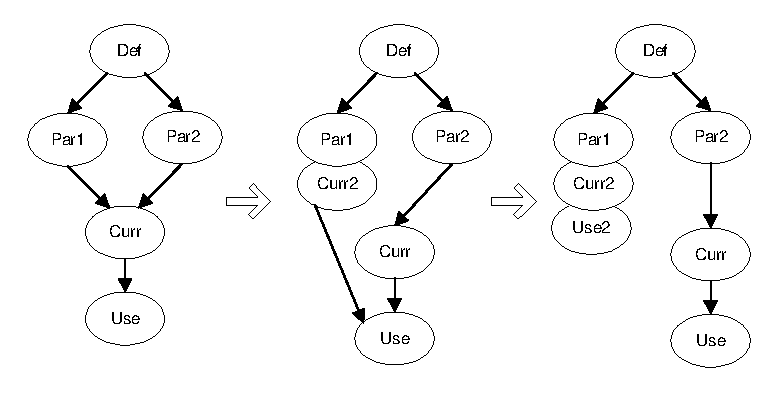
\includegraphics{figures/DuplicateBB.eps}
\centerfigend{fig-duplicateBB}{Duplicating BBs to ensure that each use of
a BasicBlock has a unique definition}

\subsection*{Duplicating a Basic Block}
When the parent of a basic block that needs to be duplicated is a fall-through
or a one-way jump BB, there is only one in-edge, so the RTLs for the current
BB are merely copied
to the end of the list of
RTLs in the parent BB. The parent BB then becomes the same type as the copied
BB, and has the same number of outedges. (The outedges are copied explicitly).
Copying of BBs is done with the clone() member function, to ensure ``deep''
copying. Otherwise, only the pointers to expressions are copied, not the
expressions themselves, and there will be problems when the expressions are
deleted (since the same expression will be deleted twice).

When the parent of a basic block that needs to be duplicated is a two-way BB,
the above method is not suitable. Instead, a new BB is created that is a clone
of the current BB, and the out-edge from the parent to the current BB is
changed to point to the new BB. (Note: this could be the first or ``true''
outedge, or it could be the second or ``false'' outedge). The back end must not
pay attention to the destination of the branch (which remains a faithful
decoding of the original source machine instruction), but rather to where the
BB that the out-edge points to.

In Figure~\ref{fig-duplicate-2way}(a), BB ``Curr'' has a parent BB (``Par1'')
which is a 2-way BB. In this case, a copy of ``Curr'' called ``Curr2'' is made
(Figure~\ref{fig-duplicate-2way}(b)), and the out-edge that used to point to
``Curr'' is changed to point to ``Curr2''. As before, this causes ``Curr2''
to have only one parent, but the successor of both ``Curr'' and ``Curr2''
(the BB ``Use'') now has two parents. When the process is applied to that BB,
we end up with the situation in Figure~\ref{fig-duplicate-2way}(c) where both
``Use'' and ``Use2'' have single paths to the defining BB (not shown).

\centerfigbegin
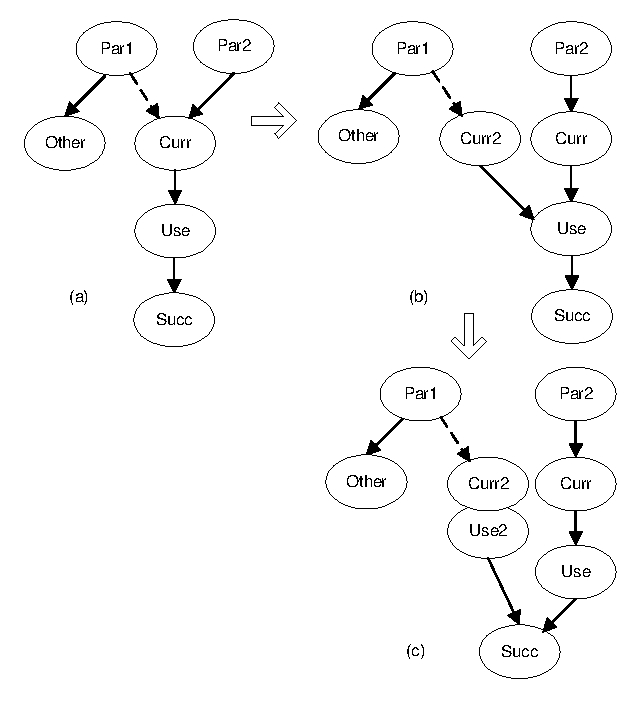
\includegraphics{figures/DuplicateBB2.eps}
\centerfigend{fig-duplicate-2way}{Duplicating a BB with a 2-way parent BB}


\section{Combining Uses and Definitions of Condition Codes}
\label{sec-comb-use-def}

Once unique pairs of CC uses and definitions are found, they must be converted
to a high level equivalent form.

\subsection{Conditional branches and set instructions}

Instructions defining the condition codes are divided into two classes:
``add-like'' and ``subtract-like''. The last RT of the RTL defining the
condition codes (which is expected to be an RTFlagCall\footnote{An object of
class RTFlagCall represents a call to a function that nominally sets the
condition codes for a family of instructions. For example, LOGICALFLAGS sets
the flags for the logical family of instructions.} object) is examined. If
the strings ``SUB'' or ``FFLAG''\footnote{Floating point compares are
considered to be always ``subtract like'', and SETFFLAGS is a typical
flag call function name for setting the floating point condition codes.}
are found in the name of the flag call function, the
instruction defining the condition codes is classified as ``subtract-like''.
Examples include compare instructions, and actual subtract instructions.
Otherwise, the instruction is classified as ``add-like''; examples include
logical instructions such as AND, multiply instructions, and actual ADD
instructions. It is therefore important that the flag call functions are
named appropriately in the SSL file (see section~\ref{sec-srd} for details).

Subtract-like definitions are handled by constructing a high level comparison
expression based on the operands of the comparison or subtraction, and the
type of branch or set instruction. For example,
\begin{verbatim}
 sub a, b, c    # Subtract b from a, result to c
 ...
 sge dest       # Set dest to 1 if "greater than or equals"
\end{verbatim}
has the following high level expression associated with it: ``a $>=$ b''.
The expression is stored in the HLJcond or HLScond object associated
with the RTL that uses the condition code. (The \texttt{setCondExpr} method is
used.)

It is not possible to use the operands directly, since in the final program,
a and b could be modified before the instruction that uses the condition codes.
A mechanism is needed to ``transport'' the condition code information from the
defining instruction to the using instruction. Variables (e.g. ``v12''),
unique to this definition-use pair, are used for this purpose.
Subtract-like definitions of the condition codes
require two such variables; one is needed for each operand.

The variables are copied from expressions passed to the HLFlagCall RT. This
ensures that the correct arguments are copied.

It is important to realise that the result of the subtract is \emph{not}
sufficient to store the result of an unsigned comparison; e.g. v12 = b \gtu\ c
and then branch if v12 \gtu\ 0. For example, 4 \gtu\ 3 and 4-3=1 \gtu\ 0. But
(using 8 bit operands) 204 \gtu\ 3, but 204-3 = 201 == -55, which is a negative
result. (Besides, everything is unsigned greater than 0, other than 0 itself).
The result of the unsigned comparison is in the carry flag, which is a sort of
9th bit of the result.  Therefore, it is not possible in general to save on
variables where unsigned comparisons are involved.

Example pairing:
\begin{verbatim}
10b84:  d0 07 bf e8        ld           [%fp - 24], %o0
10b88:  80 a4 00 08        cmp          %l0, %o0
10b8c:  1a 80 00 04        bgeu         0x10b9c
\end{verbatim}

translates to:

\begin{verbatim}
 v2=*(...);                 # %o0 is mapped to variable v2
 v30=v2;                    # Copy operand 1
 v29=r16;                   # Copy operand 2
 r0=(r16)-(v2);             # The compare, expressed as a subtract
                            #  (result is not used)
 v2=70656;                  # Delay slot instruction
 if (v29 >= v30) goto L11;  # Unsigned comparison
\end{verbatim}

By contrast, add-like definitions need only the result of the operation 
that sets the condition codes. It is an error to find unsigned branches 
or set instructions using the condition codes from an add-like definition. 
For example
\begin{verbatim}
 add a, b, c        # Add a and b, result to c
 ...
 jge dest           # Jump if "greater or equal" to dest
\end{verbatim}
becomes
\begin{verbatim}
c = a + b;
v12 = c;
 ...
if (v12 >= 0) goto dest;
\end{verbatim}

The exception to the above rules are the \texttt{HLJCOND\_JMI} and
\texttt{JLJCOND\_JPOS} branches. These can be used after add-like or after
subtract-like operations (usually a genuine subtract), but since they depend on
the result of the operation, they must be used in an add-like manner.
For example, from
\begin{verbatim}
10bec:  90 a2 20 01        subcc    %o0, 1, %o0
10bf0:  3c bf ff fa        bpos,a   0x10bd8
\end{verbatim}
we generate
\begin{verbatim}
r8=(r8)-(1);
v8=r8;
if ((v8)>=(0)) goto L3;
\end{verbatim}

The analysis code makes the assumptions that the last RT of the RTL defining
the condition codes is a flag call, and (for the above cases) that the second
last RT is an assignment to the result of the operation defining the flags.
Note that if there is a second branch that depends on the above operation,
the second last assignment will be to v8, but it still has the result of the
operation, so it will work correctly.

For other subtract-like operations and branches, it is assumed that the
first two operands (in order) of the flag call are the two operands being
compared (or subtracted). In other words, after
\begin{verbatim}
  x := y - z
  SUBFLAGS(a, b, ...)
\end{verbatim}
it is assumed that a is y and b is z.

As a result of these assumptions, the user is not free to use unusual
semantics in the SSL file. It is hard to imagine the above assumption not
being valid, but it should be kept in mind. In extreme cases, the result of
the operaton may have to be assigned to a temporary variable, then to
either the true destination or another temporary in the second last RT.

\subsection{Assignments that use Condition Codes}

When the instruction using a condition code is an assignment, it is usually
part of an idiomatic sequence.  Two idioms have so far been found and
implemented. The other class of instruction using the carry flag is as part
of multiword arithmetic (e.g. addcc, addx). It may be practical to implement
the multiword arithmetic pairs when the type analysis is able to cope with
variables in two registers; for now, these sequences generate an error message.
This example is from the Solaris 7 /usr/bin/awk:
\begin{verbatim}
142e8:  d2 07 20 00        ld           [%i4], %o1      # Load high half
142ec:  d6 07 20 04        ld           [%i4 + 4], %o3  # Load low half
...
                           # addcc sets flags according to result; add does not
14330:  b4 82 e0 01        addcc        %o3, 1, %i2     # Add 1 to low half
14334:  b2 42 60 00        addx         %o1, 0, %i1     # Add carry to top half
...
142d0:  f2 27 20 00        st           %i1, [%i4]
142d8:  f4 27 20 04        st           %i2, [%i4 + 4]
\end{verbatim}

Here, there are 64 bit integer quantities in the register pairs \%o1:\%o3,
and also \%i1:\%i2 (the colon represents concatenation).

The first idiomatic sequence is: ``compare 0 to a; use carry flag''. Arithmetic
assignment statements using the carry flag need no extra transformation; they
decode to RTLs which use the \%CF register (machine independent carry
flag). For example, \texttt{addx \%g0, 0, \%o3} decodes to
``r[10] := r[0] + 0 + \%CF''. (In the final C output of the translator, \%CF
is represented by the integer variable CF). Therefore, the only transformation
required is to ensure that each use has a unique definition, and to make an
appropriate assignment to \%CF.

Since subtracting any value from zero will generate a carry, unless that value
is zero, comparing 0 to X is equivalent to setting the carry flag only if X
is non-zero. In other words,
compare 0 to X is transformed to ``\%CF = (X != 0)''. An appropriate
assignment RT (i.e. an object of class RTAssgn) is created, and appended to the
list of RTs for the RTL defining the flags. For example:
\begin{verbatim}
10aec:  80 a0 00 0b        cmp          %g0, %o3        # %g0 is always 0
10af0:  94 60 3f ff        subx         %g0, -1, %o2    # Make use of %CF
10af8:  96 40 20 00        addx         %g0, 0, %o3     # Another use of %CF
\end{verbatim}
transforms to
\begin{verbatim}
         # Variable v5 represents register %o3 for this procedure
00010aec *32* r[0] := -v5           # The compare, expressed as a subtract
         *32* %CF := v5 ~= 0        # Generated assignment
         SUBFLAGS( r[0], v5, r[0] )
00010af0 *32* v4 := -%CF + 1        # Register %o2 is held in variable v4
00010af4 *32* v5 := %CF             # Register %o3 is held in variable v5
\end{verbatim}
In C, this becomes
\begin{verbatim}
        r0=-(v5);
        CF=(v5)!=(0);
        v4=(-(CF))+(1);
        v5=CF;
\end{verbatim}


The second idiomatic sequence is similar: ``compare X to Y; use carry flag''.
This is transformed to ``\%CF = X \ltu\ Y'' (where \ltu\ represents ``unsigned
less than''). After subtracting Y from X, a carry will be generated if and only
if Y is greater than x (with both X and Y considered as unsigned quantities).
In other words, after cmp X, Y the carry flag represents the logical expression
X \ltu\ Y.

\section{Complex example}

Despite the apparent simplicity of the above, real code can be surprisingly
complex. The following SPARC code is from the 126.gcc Spec benchmark, generated
from the last 4 lines of C here:

\begin{verbatim}
  int unsignedp = TREE_UNSIGNED (index_type);
  typedef rtx rtx_function ();
  rtx_function *gen_bgt_pat = unsignedp ? gen_bgtu : gen_bgt;
  rtx_function *gen_bge_pat = unsignedp ? gen_bgeu : gen_bge;
  rtx_function *gen_blt_pat = unsignedp ? gen_bltu : gen_blt;
  rtx_function *gen_ble_pat = unsignedp ? gen_bleu : gen_ble;
\end{verbatim}

The addresses of the eight functions (e.g. \texttt{gen\_bgtu}) are set up in
registers like \texttt{\%i2} and stack memory like \texttt{[\%sp + 144]}
in earlier code that is not relevant to the analysis.

\begin{verbatim}
7834c:  80 90 00 1b        orcc         %g0, %i3, %g0
78350:  02 80 00 04        be           0x78360
78354:  a8 10 00 1a        mov          %i2, %l4
78358:  10 80 00 02        ba           0x78360
7835c:  a8 10 00 19        mov          %i1, %l4
78360:  22 80 00 04        be,a    0x78370
78364:  e4 03 a0 90        ld           [%sp + 144], %l2
78368:  10 80 00 02        ba           0x78370
7836c:  e4 03 a0 94        ld           [%sp + 148], %l2
78370:  22 80 00 04        be,a    0x78380
78374:  e2 03 a0 98        ld           [%sp + 152], %l1
78378:  10 80 00 02        ba           0x78380
7837c:  e2 03 a0 9c        ld           [%sp + 156], %l1
78380:  02 80 00 04        be           0x78390
78384:  90 10 00 1c        mov          %i4, %o0
78388:  10 80 00 03        ba           0x78394
7838c:  a0 10 00 1d        mov          %i5, %l0
78390:  e0 03 a0 a0        ld           [%sp + 160], %l0
78394:  92 10 00 15        mov          %l5, %o1
\end{verbatim}

The orcc instruction at the top is the definition for the following conditional
branch, and also three more branches. Because of the two-way BBs between the
definition and the conditional branches, there are a lot of BB duplications
required to translate this code.

There are also several ``orphan'' basic blocks generated as a result of
untangling the delay slots in the above. The code above generates some
23 basic blocks, as shown in Figure~\ref{fig-complex-example}.

\centerfigbegin
{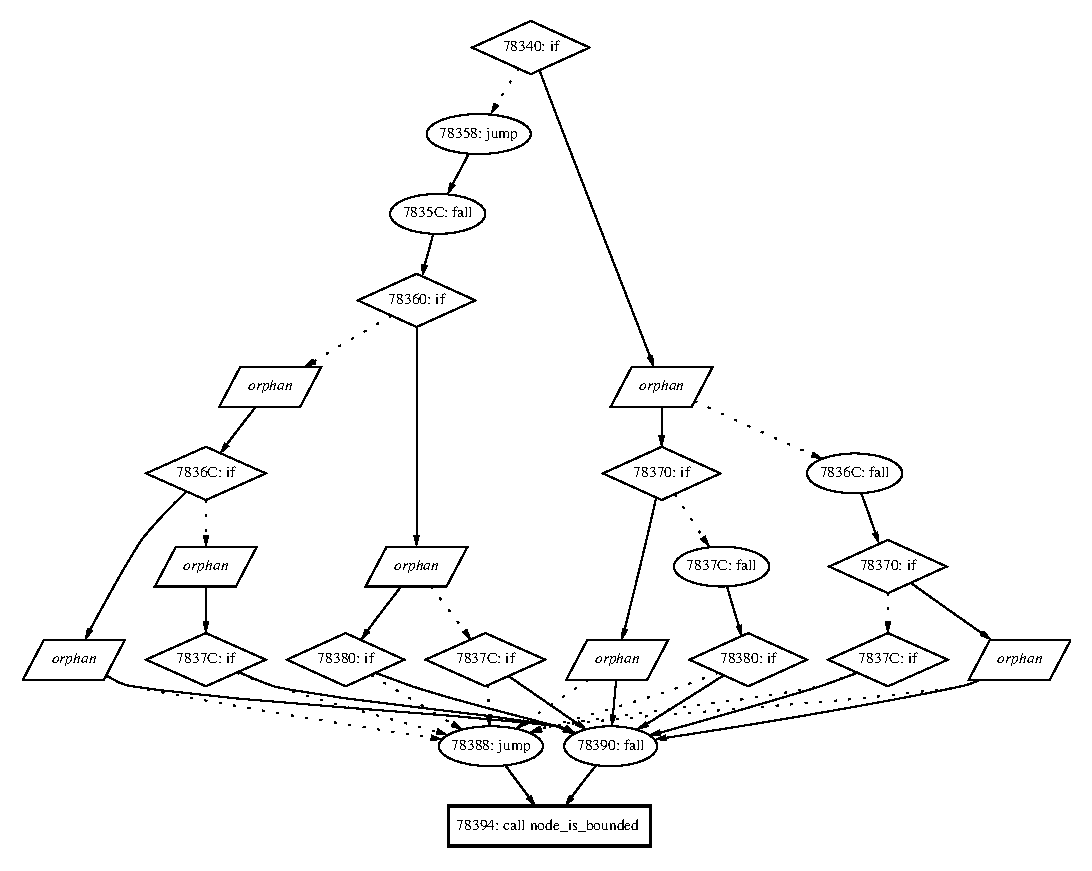
\includegraphics{figures/complex_example.eps}}
\centerfigend{fig-complex-example}{BBs generated for the complex example}
      % matching condition code definitions and uses

  	
\chapter{Transformations of Delayed Transfers of Control}
\label{ch-delay}

{\small
\begin{flushright}
Design: Norman and Cristina [c.98]; Implementation: Mike [c.98-99]; Documentation: Norman, Cristina [Sep 99]
\end{flushright}
}

This chapter is an updated version of Technical Report 440, Department of 
Computer Science and Electrical Engineering, The University of 
Queensland, December 1998.  A more up to date version, including 
application of this algorithm to the removal of PA-RISC delayed branches
will be part of a Sun Microsytems Laboratories Technical Report series  
(expected, early 2002). 
 

% l2h ignore special {% ===> this file was generated automatically by noweave --- better not edit it

%\ifx\afour\undefined
%  \documentclass[letterpaper]{elsart}
%  \let\sizeinfo\relax
%\else 
%  \documentclass[a4paper]{elsart}
%  \special{papersize=210mm,297mm} % put dvips into a4 automagically
%  \def\sizeinfo{A4 }
%\fi

%\usepackage{nchicago}

% l2h substitution bullet *
% l2h substitution and and
% l2h ignore active


\makeatletter
\def\@citex[#1]#2{%
  \let\@citea\@empty
  \@cite{\@for\@citeb:=#2\do
        {\@citea\def\@citea{,\penalty\@m\ }%
         \edef\@citeb{\expandafter\@firstofone\@citeb}%
         \if@filesw\immediate\write\@auxout{\string\citation{\@citeb}}\fi
         \@ifundefined{b@\@citeb}{\mbox{\reset@font\bfseries ?}%
           \G@refundefinedtrue
           \@latex@warning
             {Citation `\@citeb' on page \thepage \space undefined}}%
           {\citebox{\csname b@\@citeb\endcsname}}}}{#1}}
\let\citebox\hbox
\makeatother

\renewcommand\gets{\mathrel{:=}}

\newcommand\opentab{\addtolength{\extrarowheight}}
% l2h ignore catcode ==
% l2h let gdef def

% l2h substitution hatform ^
% l2h ignore markboth {{

% l2h ignore opentab {

% l2h substitution presigmap sigma'
% l2h ignore productionglue
% l2h substitution qquad &nbsp;&nbsp;&nbsp;&nbsp;&nbsp;

\newif\iffullpaper
\fullpapertrue


% l2h argblock calexp E[ ]
% l2h argblock cmd E[ ]


\newcommand\calexp[1]{{\mathcal E}[\![#1]\!]}
\newcommand\cmd[1]{{\mathcal C}[\![#1]\!]}
\newcommand\pc{\mathit{PC}}

%\usepackage{array,tabularx,grammar}

% l2h letenv production quote

\newif\iftr
\trfalse % this is not the tech report

\newcolumntype{Y}{>{\raggedright\arraybackslash}X}


%\usepackage{noweb}
\let\originalprime='
\def\setupcode{\catcode`\ =10 \catcode`\'=12 \mathcode`\'="8000 \regressprime}
{\catcode`\'=\active 
 \makeatletter
 \gdef\regressprime{\def'{^\bgroup\prim@s}}
}
\let\Tt\relax


% l2h substitution div div
% l2h substitution mod mod

\overfullrule=10pt

\noweboptions{shortxref}
\def\nwdocspar{\vskip0pt plus1.5in\penalty-400\vskip0pt plus -1.5in}
%\def\nwdocspar{\par\penalty-1000}
\def\nwendcode{\endtrivlist\endgroup} % ditches filbreak
%\def\nwendcode{\endtrivlist\endgroup\vskip\nwextraglue} % page tuning

\newcommand{\fig}[1]{Figure~\ref{fig:#1}}

\newcommand\sfilbreak[1]{\vskip 0pt plus#1\penalty-200\vskip 0pt plus -#1}

\setcounter{secnumdepth}{2}

\let\orghbox=\hbox
\newcommand\nohbox{\let\hbox=\orghbox\relax}



%% \pagestyle{myheadings}
%% \catcode`\$=10 % make $ a blank space
%% \catcode`\:=10 % make : a blank space
%% \newcommand\rcsrevision{$Revision: 1.4 $}
%% \catcode`\$=3 % dollar sign is math shift
%% \catcode`\:=12
%% \markboth{\rcsrevision: \sizeinfo Draft of \today}{\rcsrevision: \sizeinfo Draft of \today}
%% 
%% \pagestyle{plain}

\def\remark#1{\marginpar{\raggedright\hbadness=10000
        \def\baselinestretch{0.8}\scriptsize
        \it #1\par}}

\let\hatform\overline

\let\nwpphat=\hatform

The fundamental steps in binary translation are
distinguishing code from data, mapping data from source to
target, and translating instructions.
Translating instructions presents few problems, except
when the source instruction set 
has features not present in typical compiler intermediate codes.
The most common such feature is the delayed branch.

Standard code-generation technology can handle delayed branches in the
target language, but not in the source.
Translating delayed branches can involve tricky case
analyses to figure out what happens if there is a branch instruction in
a delay slot.
This chapter presents a disciplined method for deriving such case analyses.
The method identifies problematic cases,
shows the translations for the non-problematic cases, and gives
confidence that all cases are considered.
The method also applies to other tools that analyze machine instructions.

We begin by writing a very simple interpreter for the source machine.
It specifies, at the register-transfer level, how the source machine
executes instructions, including delayed branches. We then transform
the interpreter into an interpreter for a target machine without
delayed branches.
To maintain the semantics of the program being interpreted, we 
simultaneously transform the sequence of source-machine instructions
into a sequence of target-machine instructions.
The transformation of the instructions becomes our
algorithm for binary translation.

We show the translation is correct by using a correspondence between
source and target states, and showing if the source and target
machines begin execution in corresponding states, they reach new
corresponding states in a few instructions.


\renewcommand\opencite[1]{{\let\citebox=\relax\cite{#1}}}

A quick reading of this chapter might suggest that the problem we solve
is trivial.
To build a flow graph representing a binary program,
why not simply convert the delayed branch to a non-delayed branch and
push the instruction in the delay slot along zero, one, or both
sucessor edges?
(The set of successors that should get copies of the instruction in
the delay slot depends on whether the delayed branch
``annuls'' that instruction.)
This simple approach is in fact correct, \emph{except} when the
instruction in the delay slot is itself a delayed branch.
In that case, the ``pushing'' approach fails to execute the
instruction that is the target of the first branch.
The methods in this paper translate this case correctly.
In practice, such cases occur rarely in user code, but they are
recommended in kernel code as a way of returning from interrupts or
otherwise switching contexts \cite[\S B.26]{sparc:architecture}.


\section{Semantic framework}

Rather than translate source-machine instructions directly into target-machine
instructions, we translate source instructions into register transfer
lists (RTLs), transform the RTLs, optimize the RTLs, and translate the
RTLs into target-machine instructions.
RTLs provide a uniform framework that can express source instructions,
target instructions, and their interpretations by the source and
target processors.

\subsection{Register transfer lists}

Our RTL formalism is designed for use in tools and component
generators, and it makes machine-dependent
computation explicit \opencite{ramsey:embedded}.
For this paper, we use a simplified version specified using an imperative syntax:
\begin{production}{rtl}%figure
\optional{\nt{effect} \sequence{\lit\vbar\ \nt{effect}}}
&Multiple assignment
\end{production}
\productionglue
\begin{production}{effect}%figure
\optional{\nt{exp} {{\Tt{}\(\mathbin{\rightarrow}\)}}} \nt{location} := \nt{exp}&
Guarded assignment
\end{production}
\productionglue
\begin{production}{exp}%figure
\term{constant}&Constant
| \nt{location}&Fetch from a location
| \nt{exp} \nt{binop} \nt{exp}&Binary RTL operator
| \nt{operator} \lit( \nt{explist} \lit)&RTL operator
\end{production}
A register transfer list is a list of guarded effects.
Each effect represents the transfer of a value into a storage
location,\footnote{Storage locations represent not only memory but
also registers and other processor state.}
 i.e., a store
operation.
The transfer takes place only if the guard (an expression) evaluates
to \textbf{true}.
Effects in a list take place simultaneously, as in
Dijkstra's multiple-assignment statement; an RTL represents a single
change of state.
%%For example, one RTL can specify a swap instruction without
%%introducing bogus temporaries.

Values are computed by expressions without
side effects.
Eliminating side effects simplifies analysis and transformation.
Expressions may be integer constants, fetches from locations, or
applications of \emph{RTL operators} to lists of expressions.
RTL operators are pure functions on values.

For purposes of this paper, we assume that locations are single cells
in a mutable store, although the RTL formalism supports a more general
view that makes byte order explicit.
\iffalse
Locations may be single cells or aggregates of consecutive
cells within a storage space.
Aggregation generalizes the idea of byte order, specifying a bijection
between a contiguous sequence of $k$ $n$-bit values and a single
$w$-bit value, where $w = kn$.\footnote{$w$ and $n$ are mnemonic for
``wide'' and ``narrow.''}
\fi

\iffullpaper
As an example of a typical RTL, consider a SPARC load instruction
using the displacement 
addressing mode, written in the SPARC  assembly language as
\begin{verbatim}
  ld [%sp-12], %i0
\end{verbatim}
The effect of this load instruction might be written
\nwenddocs{}\nwbegincode{2}\moddef{RTL for sample instruction}\endmoddef\nwstartdeflinemarkup\nwenddeflinemarkup
\(\$r[24] \mathrel{:=} \$m[\$r[14]+{\mathit{sx}}(\mathord{-}12)]\)
\nwendcode{}\nwbegindocs{3}because the stack pointer is register~14 and register \texttt{\%i0} is
register~24.
The notation {\Tt{}\(\$\)}\emph{space}\texttt{[}\emph{address}\texttt{]}
specifies a cell in a mutable store.
The {\Tt{}\({\mathit{sx}}\)} operator sign-extends the 13-bit immediate constant {\Tt{}\(\mathord{-}12\)}
so it can be added to the 32-bit value fetched from register~14.

The load instruction not only loads a value into register~24; it also advances
the program counter to point to the next instruction.
Changing the program counter is intimately connected with branching;
we separate the effect on the
program counter in order to give it special treatment.
\else
\emph{The full paper shows and explains an example RTL.}
\fi

\subsection{Processor state for delayed branches}

A processor executing straight-line code executes one instruction
after another, in sequence.
A delayed-branch instruction causes the processor to depart from that
sequence, but not immediately.
When the processor executes an instruction~{\Tt{}\(I\)} that causes a delayed
branch to a location 
{\Tt{}\({\mathit{target}}\)}, the processor {first} executes {\Tt{}\(I\)}'s successor,
{then} executes the instruction located at {\Tt{}\({\mathit{target}}\)}.
The location holding {\Tt{}\(I\)}'s successor is called {\Tt{}\(I\)}'s ``delay
slot.''
On some machines, like the SPARC,
the instruction~{\Tt{}\(I\)} can
``annul'' its successor, in which case the successor is
\emph{not} executed, but instead the processor stalls for a cycle
before transferring control to {\Tt{}\({\mathit{target}}\)}.

To model delayed branches with annuls, we use
three pieces of processor state:
\begin{itemize}
\item[{}{\Tt{}\({\mathit{PC}}\)}{}] is the program counter, which identifies the
instruction about to be executed.
\item[{}{\Tt{}\({\mathit{nPC}}\)}{}] is the ``next program counter,'' which identifies the
instruction to be executed after the current instruction.
\item[{}{\Tt{}\({\mathit{annul}}\)}{}] is the ``annul status,'' which determines
whether the processor executes the instruction at~{\Tt{}\({\mathit{PC}}\)} or ignores
it.%
\footnote{\iffullpaper
It is crucial to distinguish the {\Tt{}\({\mathit{annul}}\)} status, which is
part of 
the processor state, from the \texttt{a}~bit found in the binary
representations of some branch instructions.
The interpretation of the {\Tt{}\({\mathit{annul}}\)} status is trivial: it tells
directly whether to execute an instruction.
The interpretation of the \texttt{a}~bit (when present) is more involved,
because there are special rules for some instructions.
We abstract away from these special rules by associating with each
instruction~{\Tt{}\(I\)} a predicate~{\Tt{}\(a_I\)} (not necessarily a single bit) that
tells the processor 
whether to annul the instruction's successor.
\else
\emph{The full paper notes the distinction between {\Tt{}\({\mathit{annul}}\)} and the
\texttt{a}~bit found in some branch instructions.}%
\fi
}
\end{itemize}
In this model, a delayed control transfer is represented by an
assignment to~{\Tt{}\({\mathit{nPC}}\)}.
For example, a SPARC call instruction simultaneously
assigns the target address to~{\Tt{}\({\mathit{nPC}}\)}
and the current {\Tt{}\({\mathit{PC}}\)} to register~15:
\nwenddocs{}\nwbegincode{4}\moddef{RTL for call}\endmoddef\nwstartdeflinemarkup\nwenddeflinemarkup
\({\mathit{nPC}} \mathrel{:=} {\mathit{target}} \mathrel{|} \$r[15] \mathrel{:=} {\mathit{PC}}\)
\nwendcode{}\nwbegindocs{5}The {\Tt{}\({\mathit{target}}\)} address in the semantics is
distinct from the \texttt{target} field in the binary representation of the
call instruction.
In the case of the SPARC, we abstract away from the rule that says the
target 
address is computed by extending the \texttt{target} field on the
right with zeroes.

A call transfers control unconditionally; we represent a conditional
branch by a guarded assignment to {\Tt{}\({\mathit{nPC}}\)}.
The \texttt{BNE} (branch not equal) instruction tests the {\Tt{}\(Z\)}~(zero)
bit in the condition codes:
\nwenddocs{}\nwbegincode{6}\moddef{rtl for conditional branch \texttt{BNE}}\endmoddef\nwstartdeflinemarkup\nwenddeflinemarkup
\(\lnot  Z \mathbin{\rightarrow} {\mathit{nPC}} \mathrel{:=} {\mathit{target}}\)
\nwendcode{}\nwbegindocs{7}Again we abstract the computation of the target address relative to
the location of the instruction.
\nwenddocs{}\nwbegindocs{8}\nwdocspar
\subsection{A canonical form of RTLs}
To isolate the part of instruction semantics that is relevant to
control flow, we put RTLs into the following canonical form:
\nwenddocs{}\nwbegincode{9}\moddef{RTL for generic instruction \code{}I\edoc{}}\endmoddef\nwstartdeflinemarkup\nwenddeflinemarkup
\(b_I \mathbin{\rightarrow} {\mathit{nPC}} \mathrel{:=} {\mathit{target}}_I \mathrel{|} {\mathit{annul}} \mathrel{:=} a_I \mathrel{|} I_c\)
\nwendcode{}\nwbegindocs{10}We interpret this form as follows:
\begin{itemize}
\item [{}{\Tt{}\(b_I\)}{}] is a predicate that tells whether {\Tt{}\(I\)}~branches.
It is an \emph{expression}, not a constant or a field of the
instruction.
For non-branching instructions, {\Tt{}\(b_I\)}~is {\Tt{}\(\textbf{false}\)}.
For calls and
unconditional branches, {\Tt{}\(b_I\)} is {\Tt{}\(\textbf{true}\)}.
For conditional branches, {\Tt{}\(b_I\)} is some other expression, the value of
which depends on the state of the machine (e.g., on the values of
the condition codes).
\item [{}{\Tt{}\({\mathit{target}}_I\)}{}] is an {expression} that identifies the
target address to which {\Tt{}\(I\)}~may branch.
(If {\Tt{}\(b_I\)} is {\Tt{}\(\textbf{false}\)}, {\Tt{}\({\mathit{target}}_I\)} is arbitrary.)
For calls and PC-relative branches, {\Tt{}\({\mathit{target}}_I\)} is a constant that
statically identifies a target address.
For indirect branches, {\Tt{}\({\mathit{target}}_I\)} may be a more complex expression,
e.g., one that fetches an address stored in a register.
\item [{}{\Tt{}\(a_I\)}{}] is a predicate that tells whether {\Tt{}\(I\)}~annuls its
successor. 
It is an expression, {not} the value of the \texttt{a}~bit in an
instruction's representation.
For most instructions, {\Tt{}\(a_I\)} is {\Tt{}\(\textbf{false}\)}.
For conditional branches, {\Tt{}\(a_I\)} may be more complicated.
For example,  the SPARC \texttt{BNE} instruction annuls its successor
if the \texttt{a} bit is set and if the branch is not taken, so {\Tt{}\(a_I\)} is
\mbox{{\Tt{}\(\mathtt{a} \ne  0 \land  Z\)}}.
\item [{}{\Tt{}\(I_c\)}{}] is an RTL that represents {\Tt{}\(I\)}'s ``computational
effect.''
{\Tt{}\(I_c\)} may be empty, or it may contain guarded assignments that do
not change {\Tt{}\({\mathit{annul}}\)}, {\Tt{}\({\mathit{nPC}}\)}, or {\Tt{}\({\mathit{PC}}\)}.
Typical RISC instructions change control flow or perform computation,
but not both, so {\Tt{}\(I_c\)} tends to be non-empty only when {\Tt{}\(b_I\)}
and {\Tt{}\(a_I\)} are {\Tt{}\(\textbf{false}\)}.
On CISC architectures, however, an instruction like ``decrement and
skip if zero'' might have both  non-empty {\Tt{}\(I_c\)} (the decrement) and
a nontrivial {\Tt{}\(b_I\)} (the test for zero).
\end{itemize}
An instruction can be expressed in this canonical form if, when
executed, it branches to
at most one {\Tt{}\({\mathit{target}}\)}.%
\footnote{And of course if the machine uses delayed branches.}
This is true of all instructions on all architectures with which we
are 
familiar, including indirect-branch instructions (although the value
 of {\Tt{}\({\mathit{target}}\)} may be different on different executions of an indirect
branch).

Here are a few example RTLs in canonical form;
SPARC assembly language appears on the left, RTLs on the right.
{\Tt{}\textbf{skip}} is the empty~RTL.
\begin{quote}%figure
\begin{tabular}{@{}ll@{}}
\multicolumn2{@{}l}{\texttt{add rs1, rs2, rd}}\\
\multicolumn2{@{}l}{\qquad  
{\Tt{}\(\textbf{false} \mathbin{\rightarrow} {\mathit{nPC}} \mathrel{:=} {\mathit{any}} \mathrel{|} {\mathit{annul}} \mathrel{:=} \textbf{false} \mathrel{|} \$r[\mathtt{rd}] \mathrel{:=} \$r[\mathtt{rs1}] + \$r[\mathtt{rs2}]\)}}\\
\texttt{ba,a addr}&{\Tt{}\(\textbf{true} \mathbin{\rightarrow} {\mathit{nPC}} \mathrel{:=} \mathtt{addr} \mathrel{|} {\mathit{annul}} \mathrel{:=} \textbf{true} \mathrel{|}\){\ }\textbf{skip}}\\
\texttt{call addr}&{\Tt{}\(\textbf{true} \mathbin{\rightarrow} {\mathit{nPC}} \mathrel{:=} \mathtt{addr} \mathrel{|} {\mathit{annul}} \mathrel{:=} \textbf{false} \mathrel{|} \$r[15] \mathrel{:=} {\mathit{PC}}\)}\\
\end{tabular}\kern-20pt
\end{quote}

\nwenddocs{}\nwbegindocs{11}\nwdocspar
\subsection{Instruction decoding and execution on two platforms}
Given this canonical form for instructions, we represent instruction
decoding using a {\Tt{}\textbf{let}}-binding notation:
\nwenddocs{}\nwbegincode{12}\moddef{instruction decoding}\endmoddef\nwstartdeflinemarkup\nwenddeflinemarkup
\textbf{let}{\ }\((b_I \mathbin{\rightarrow} {\mathit{nPC}} \mathrel{:=} {\mathit{target}}_I \mathrel{|} {\mathit{annul}} \mathrel{:=} a_I \mathrel{|} I_c) \equiv  {\mathit{src}}[{\mathit{PC}}]\)
\textbf{in}{\ }{\ }\(\ldots\)
\textbf{end}
\nwendcode{}\nwbegindocs{13}The {\Tt{}\textbf{let}} construct binds {\Tt{}\(b_I\)}, {\Tt{}\({\mathit{target}}_I\)},
{\Tt{}\(a_I\)}, and {\Tt{}\(I_c\)}, which together determine the
semantics of the instruction~{\Tt{}\(I\)} found in the source memory~{\Tt{}\({\mathit{src}}\)}.
\iffullpaper
This {\Tt{}\textbf{let}}-binding represents not only the process of using the
binary representation to identify the instruction and its operands,
but also the abstraction from that representation into the RTL semantics.
This abstraction from binary representation to semantics can be done
statically, at 
binary-translation time; it can even be automated based on a
combination of machine descriptions
\opencite{ramsey:specifying,ramsey:embedded}.
\fi
\nwenddocs{}\nwbegindocs{14}\nwdocspar
The source-machine execution loop
decodes an instruction and executes it as follows:
\nwenddocs{}\nwbegincode{15}\moddef{sparc execution loop}\endmoddef\nwstartdeflinemarkup\nwenddeflinemarkup
\textbf{fun}{\ }\({\mathit{loop}} () \equiv \)
{\ }{\ }\textbf{let}{\ }\((b_I \mathbin{\rightarrow} {\mathit{nPC}} \mathrel{:=} {\mathit{target}}_I \mathrel{|} {\mathit{annul}} \mathrel{:=} a_I \mathrel{|} I_c) \equiv  {\mathit{src}}[{\mathit{PC}}]\)
{\ }{\ }\textbf{in}{\ }{\ }\textbf{if}{\ }\({\mathit{annul}}\){\ }\textbf{then}
{\ }{\ }{\ }{\ }{\ }{\ }{\ }{\ }{\ }\({\mathit{PC}} \mathrel{:=} {\mathit{nPC}} \mathrel{|} {\mathit{nPC}} \mathrel{:=} {\mathit{succ}}_s({\mathit{nPC}}) \mathrel{|} {\mathit{annul}} \mathrel{:=} \textbf{false}\)
{\ }{\ }{\ }{\ }{\ }{\ }\textbf{else}{\ }\textbf{if}{\ }\([\![b_I]\!]\){\ }\textbf{then}
{\ }{\ }{\ }{\ }{\ }{\ }{\ }{\ }{\ }\({\mathit{PC}} \mathrel{:=} {\mathit{nPC}} \mathrel{|} {\mathit{nPC}} \mathrel{:=} [\![{\mathit{target}}_I]\!]  \mathrel{|} [\![I_c]\!] \mathrel{|} {\mathit{annul}} \mathrel{:=} [\![a_I]\!]\)
{\ }{\ }{\ }{\ }{\ }{\ }\textbf{else}
{\ }{\ }{\ }{\ }{\ }{\ }{\ }{\ }{\ }\({\mathit{PC}} \mathrel{:=} {\mathit{nPC}} \mathrel{|} {\mathit{nPC}} \mathrel{:=} {\mathit{succ}}_s({\mathit{nPC}}) \mathrel{|} [\![I_c]\!] \mathrel{|} {\mathit{annul}} \mathrel{:=} [\![a_I]\!]\)
{\ }{\ }{\ }{\ }{\ }{\ }\textbf{fi}
{\ }{\ }{\ }{\ }{\ }{\ }\(; {\mathit{loop}}()\)
{\ }{\ }\textbf{end}
\nwendcode{}\nwbegindocs{16}We specify the repeated execution of the processor loop as a tail
call, rather than as a loop, because that simplifies the
program transformations to follow.
\nwenddocs{}\nwbegindocs{17}\nwdocspar
The notation {\Tt{}\([\![\bullet ]\!]\)} represents execution; for example,
{\Tt{}\([\![b_I]\!]\)} is the value of the branch condition, given the current
state of the machine.
Executing the computational effect {\Tt{}\([\![I_c]\!]\)} changes the state of the machine.
\nwenddocs{}\nwbegindocs{18}\nwdocspar
The function {\Tt{}\({\mathit{succ}}_s\)} abstracts over the details of identifying
the successor instruction on the source machine; {\Tt{}\({\mathit{succ}}_t\)} finds the
successor on the target machine.
In both cases, {\Tt{}\({\mathit{succ}}\)} is computed as part of instruction decoding.
\nwenddocs{}\nwbegindocs{19}\nwdocspar
Our example target, the Pentium, has neither delayed branches nor
annulling, so it has a simpler canonical form and a simpler execution
loop:
\nwenddocs{}\nwbegincode{20}\moddef{Pentium execution loop}\endmoddef\nwstartdeflinemarkup\nwenddeflinemarkup
\textbf{fun}{\ }\({\mathit{simple}} () \equiv \)
{\ }{\ }\textbf{let}{\ }\((b_I \mathbin{\rightarrow} {\mathit{PC}} \mathrel{:=} {\mathit{target}}_I \mathrel{|} I_c) \equiv  {\mathit{tgt}}[{\mathit{PC}}]\)
{\ }{\ }\textbf{in}{\ }{\ }\textbf{if}{\ }\([\![b_I]\!]\){\ }\textbf{then}
{\ }{\ }{\ }{\ }{\ }{\ }{\ }{\ }\({\mathit{PC}} \mathrel{:=} [\![{\mathit{target}}_I]\!] \mathrel{|} [\![I_c]\!]\)
{\ }{\ }{\ }{\ }{\ }{\ }\textbf{else}
{\ }{\ }{\ }{\ }{\ }{\ }{\ }{\ }\({\mathit{PC}} \mathrel{:=} {\mathit{succ}}_t({\mathit{PC}}) \mathrel{|} [\![I_c]\!]\)
{\ }{\ }{\ }{\ }{\ }{\ }\textbf{fi}
{\ }{\ }{\ }{\ }{\ }{\ }\(; {\mathit{simple}}()\)
{\ }{\ }\textbf{end}
\nwendcode{}\nwbegindocs{21}\nwdocspar




\subsection{Strategy for translating delayed branches}

Both our formalism and
the SPARC architecture manual give a clear semantics of delayed
branches in terms of {\Tt{}\({\mathit{PC}}\)}, {\Tt{}\({\mathit{nPC}}\)}, and {\Tt{}\({\mathit{annul}}\)}.
To get an efficient target program, however, we wish \emph{not} to
represent the source {\Tt{}\({\mathit{PC}}\)}, {\Tt{}\({\mathit{nPC}}\)}, and {\Tt{}\({\mathit{annul}}\)} explicitly, but to
make all three \emph{implicit} in the value of the target~{\Tt{}\({\mathit{PC}}\)}.
How to do this based on the information in the architecture manual is
not immediately obvious, but our semantic framework enables a new technique.
We transform {\Tt{}\({\mathit{loop}}\)}, eliminating {\Tt{}\({\mathit{nPC}}\)} and {\Tt{}\({\mathit{annul}}\)} wherever
possible, so that (almost all of) {\Tt{}\({\mathit{loop}}\)} can be expressed using only
the~{\Tt{}\({\mathit{PC}}\)}.
%%This transformation leads to suitable changes in the sequence of
%%instructions executed, thus guiding a transformation from {\Tt{}\({\mathit{src}}\)} to {\Tt{}\({\mathit{tgt}}\)}.
%%This latter transformation is an algorithm for binary translation of
%%delayed-branch instructions.


% l2h substitution src s-sigma-
% l2h substitution tgt t-sigma-

\newcommand\presigma[1]{\mathord{{}^{#1}\sigma}}
\newcommand\presigmap[1]{\mathord{{}^{#1}\sigma'}}
\newcommand\src[1]{\presigma{s}_{#1}}
\newcommand\tgt[1]{\presigma{t}_{#1}}


\section{Transforming the execution loop}

We wish to develop a translation function that we can point at a
location {\Tt{}\({\mathit{src}}[{\mathit{pc}}_s]\)} and that will produce suitable instructions at a
corresponding target location {\Tt{}\({\mathit{tgt}}[{\mathit{pc}}_t]\)}.
We cannot simply have {\Tt{}\({\mathit{pc}}_t = {\mathit{pc}}_s\)}; source program counters
cannot be identical to target program counters, because 
source and target instruction sequences may be different sizes.
During translation, we build {\Tt{}\({\mathit{codemap}}\)}, a map that relates program
counters on the two machines, so {\Tt{}\({\mathit{pc}}_t = {\mathit{codemap}}({\mathit{pc}}_s)\)}.

We assume that
when the source processor starts executing code at {\Tt{}\({\mathit{src}}[{\mathit{pc}}_s]\)}, it
is not in the middle of a delayed
or annulled branch, or formally,
\begin{quote}
{\Tt{}\({\mathit{annul}} = \textbf{false} \land  {\mathit{nPC}} = {\mathit{succ}}_s({\mathit{PC}})\)}.
\end{quote}
Software conventions guarantee that
the processor will be in such a state at a program's start location
and at procedure entry points.
\nwenddocs{}\nwbegindocs{22}\nwdocspar
We begin our transformation by
defining a function {\Tt{}\({\mathit{stable}}\)} that can be substituted for {\Tt{}\({\mathit{loop}}\)}
whenever {\Tt{}\({\mathit{annul}} = \textbf{false} \land  {\mathit{nPC}} = {\mathit{succ}}_s({\mathit{PC}})\)}.
\nwenddocs{}\nwbegincode{23}\moddef{stable execution loop}\endmoddef\nwstartdeflinemarkup\nwenddeflinemarkup
\textbf{fun}{\ }\({\mathit{stable}} () \equiv \)
{\ }{\ }\({\mathit{annul}} \mathrel{:=} \textbf{false} \mathrel{|} {\mathit{nPC}} \mathrel{:=} {\mathit{succ}}_s({\mathit{PC}});\)
{\ }{\ }\textbf{let}{\ }\((b_I \mathbin{\rightarrow} {\mathit{nPC}} \mathrel{:=} {\mathit{target}}_I \mathrel{|} {\mathit{annul}} \mathrel{:=} a_I \mathrel{|} I_c) \equiv  {\mathit{src}}[{\mathit{PC}}]\)
{\ }{\ }\textbf{in}{\ }{\ }\textbf{if}{\ }\({\mathit{annul}}\){\ }\textbf{then}
{\ }{\ }{\ }{\ }{\ }{\ }{\ }{\ }{\ }\({\mathit{PC}} \mathrel{:=} {\mathit{nPC}} \mathrel{|} {\mathit{nPC}} \mathrel{:=} {\mathit{succ}}_s({\mathit{nPC}}) \mathrel{|} {\mathit{annul}} \mathrel{:=} \textbf{false}\)
{\ }{\ }{\ }{\ }{\ }{\ }\textbf{else}{\ }\textbf{if}{\ }\([\![b_I]\!]\){\ }\textbf{then}
{\ }{\ }{\ }{\ }{\ }{\ }{\ }{\ }{\ }\({\mathit{PC}} \mathrel{:=} {\mathit{nPC}} \mathrel{|} {\mathit{nPC}} \mathrel{:=} [\![{\mathit{target}}_I]\!]  \mathrel{|} [\![I_c]\!] \mathrel{|} {\mathit{annul}} \mathrel{:=} [\![a_I]\!]\)
{\ }{\ }{\ }{\ }{\ }{\ }\textbf{else}
{\ }{\ }{\ }{\ }{\ }{\ }{\ }{\ }{\ }\({\mathit{PC}} \mathrel{:=} {\mathit{nPC}} \mathrel{|} {\mathit{nPC}} \mathrel{:=} {\mathit{succ}}_s({\mathit{nPC}}) \mathrel{|} [\![I_c]\!] \mathrel{|} {\mathit{annul}} \mathrel{:=} [\![a_I]\!]\)
{\ }{\ }{\ }{\ }{\ }{\ }\textbf{fi}
{\ }{\ }{\ }{\ }{\ }{\ }\(; {\mathit{loop}}()\)
{\ }{\ }\textbf{end}
\nwendcode{}\nwbegindocs{24}\nwdocspar
\iftr
We move the initial assignment inside the {\Tt{}\textbf{let}}, and we distribute
the tail call to {\Tt{}\({\mathit{loop}}\)} over the arms of the {\Tt{}\textbf{if}}.
\nwenddocs{}%
%
%
%
%
%
%
%
%
%
%
%
%
%
%
\nwbegindocs{26}\nwdocspar
We drop the first arm of the {\Tt{}\textbf{if}}, because {\Tt{}\({\mathit{annul}}\)} is always
false.
We expand the final arm by inserting a test on {\Tt{}\([\![a_I]\!]\)}.
\nwenddocs{}%
%
%
%
%
%
%
%
%
%
%
%
%
%
%
\nwbegindocs{28}\nwdocspar
The last arm of the {\Tt{}\textbf{if}} shows the proper translation of an
instruction that neither branches nor annuls.
We can substitute {\Tt{}\({\mathit{stable}}\)} for {\Tt{}\({\mathit{loop}}\)}, then drop the assignments
to {\Tt{}\({\mathit{annul}}\)} and {\Tt{}\({\mathit{nPC}}\)}, because they don't reach any uses.
Finally, we propagate the initial definition of {\Tt{}\({\mathit{nPC}}\)} to its uses.
(This should be rewritten in a final TR.)
\nwenddocs{}%
%
%
%
%
%
%
%
%
%
%
%
%
%
%
\nwbegindocs{30}\nwdocspar
The next steps are to drop the dead assignments to {\Tt{}\({\mathit{annul}}\)} and
{\Tt{}\({\mathit{nPC}}\)}, and
\fi
We do not show every step in the
transformation of {\Tt{}\({\mathit{stable}}\)}.
The first transformations move the initial
assignments inside the {\Tt{}\textbf{let}}, propagate (by forward substitution)
the assignments to {\Tt{}\({\mathit{annul}}\)} and {\Tt{}\({\mathit{nPC}}\)},
move {\Tt{}\({\mathit{loop}}\)} inside the {\Tt{}\textbf{if}},  replace {\Tt{}\({\mathit{loop}}\)}
with {\Tt{}\({\mathit{stable}}\)} where possible, and drop the (now dead)
assignments.
The result is:
\nwenddocs{}\nwbegincode{31}\moddef{stable execution loop}\plusendmoddef\nwstartdeflinemarkup\nwenddeflinemarkup
\textbf{fun}{\ }\({\mathit{stable}} () \equiv \)
{\ }{\ }\textbf{let}{\ }\((b_I \mathbin{\rightarrow} {\mathit{nPC}} \mathrel{:=} {\mathit{target}}_I \mathrel{|} {\mathit{annul}} \mathrel{:=} a_I \mathrel{|} I_c) \equiv  {\mathit{src}}[{\mathit{PC}}]\)
{\ }{\ }\textbf{in}{\ }{\ }\textbf{if}{\ }\([\![b_I]\!]\){\ }\textbf{then}
{\ }{\ }{\ }{\ }{\ }{\ }{\ }{\ }{\ }\({\mathit{PC}} \mathrel{:=} {\mathit{succ}}_s({\mathit{PC}}) \mathrel{|} {\mathit{nPC}} \mathrel{:=} [\![{\mathit{target}}_I]\!]  \mathrel{|} [\![I_c]\!] \mathrel{|} {\mathit{annul}} \mathrel{:=} [\![a_I]\!]\)
{\ }{\ }{\ }{\ }{\ }{\ }{\ }{\ }{\ }\(; {\mathit{loop}}()\)
{\ }{\ }{\ }{\ }{\ }{\ }\textbf{else}{\ }\textbf{if}{\ }\([\![a_I]\!]\){\ }\textbf{then}
{\ }{\ }{\ }{\ }{\ }{\ }{\ }{\ }{\ }\({\mathit{PC}} \mathrel{:=} {\mathit{succ}}_s({\mathit{PC}}) \mathrel{|} {\mathit{nPC}} \mathrel{:=} {\mathit{succ}}_s({\mathit{succ}}_s({\mathit{PC}})) \mathrel{|} [\![I_c]\!] \mathrel{|} {\mathit{annul}} \mathrel{:=} \textbf{true}\)
{\ }{\ }{\ }{\ }{\ }{\ }{\ }{\ }{\ }\(; {\mathit{loop}}()\)
{\ }{\ }{\ }{\ }{\ }{\ }\textbf{else}
{\ }{\ }{\ }{\ }{\ }{\ }{\ }{\ }{\ }\({\mathit{PC}} \mathrel{:=} {\mathit{succ}}_s({\mathit{PC}}) \mathrel{|} [\![I_c]\!]\)
{\ }{\ }{\ }{\ }{\ }{\ }{\ }{\ }{\ }\(; {\mathit{stable}}()\)
{\ }{\ }{\ }{\ }{\ }{\ }\textbf{fi}
{\ }{\ }\textbf{end}
\nwendcode{}\nwbegindocs{32}%
\iftr
\else 
The last arm of the {\Tt{}\textbf{if}} shows the execution of an
instruction that never branches or annuls.
It corresponds to
the execution of a similar instruction on the {\Tt{}\({\mathit{simple}}\)} target.
\fi
\nwenddocs{}\nwbegindocs{33}\nwdocspar

The next step is to unfold {\Tt{}\({\mathit{loop}}\)} in the first
and second arms of the {\Tt{}\textbf{if}} statement. 
In the second arm, {\Tt{}\({\mathit{annul}}\)} is {\Tt{}\(\textbf{true}\)}, so the call to {\Tt{}\({\mathit{loop}}()\)} can
be replaced by
{\Tt{}\({\mathit{PC}} \mathrel{:=} {\mathit{nPC}}; {\mathit{nPC}} \mathrel{:=} {\mathit{succ}}_s({\mathit{nPC}}); {\mathit{stable}}()\)}.
The definition of {\Tt{}\({\mathit{stable}}\)} reduces to
\iftr
\nwenddocs{}%
%
%
%
%
%
%
%
%
%
%
%
%
%
%
%
%
%
%
%
%
%
%
%
%
%
\nwbegindocs{35}\nwdocspar
We now simplify {\Tt{}\({\mathit{stable}}\)} in two ways.
We encapsulate the first branch of the {\Tt{}\textbf{if}} in the chunk 
{\Tt{}\LA{}case where \code{}I\edoc{} branches\RA{}}, and we simplify the
second branch.
Reasonable care is required when substituting forward the value
({\Tt{}\({\mathit{succ}}_s({\mathit{succ}}_s({\mathit{PC}}))\)}) of {\Tt{}\({\mathit{nPC}}\)}, because the 
RTL that assigns to {\Tt{}\({\mathit{nPC}}\)} also assigns to {\Tt{}\({\mathit{PC}}\)}.
Moreover, because the values bound in the {\Tt{}\textbf{let}} don't reach any
uses, the entire {\Tt{}\textbf{let}} goes away.
Finally, the call to {\Tt{}\({\mathit{loop}}\)} can be replaced by a call to {\Tt{}\({\mathit{stable}}\)},
and the dead assignments to {\Tt{}\({\mathit{annul}}\)} and {\Tt{}\({\mathit{nPC}}\)} dropped.
\fi
\nwenddocs{}\nwbegincode{36}\moddef{stable execution loop}\plusendmoddef\nwstartdeflinemarkup\nwenddeflinemarkup
\textbf{fun}{\ }\({\mathit{stable}} () \equiv \)
{\ }{\ }\textbf{let}{\ }\((b_I \mathbin{\rightarrow} {\mathit{nPC}} \mathrel{:=} {\mathit{target}}_I \mathrel{|} {\mathit{annul}} \mathrel{:=} a_I \mathrel{|} I_c) \equiv  {\mathit{src}}[{\mathit{PC}}]\)
{\ }{\ }\textbf{in}{\ }{\ }\textbf{if}{\ }\([\![b_I]\!]\){\ }\textbf{then}
{\ }{\ }{\ }{\ }{\ }{\ }{\ }{\ }{\ }\LA{}case where \code{}I\edoc{} branches\RA{}
{\ }{\ }{\ }{\ }{\ }{\ }\textbf{else}{\ }\textbf{if}{\ }\([\![a_I]\!]\){\ }\textbf{then}
{\ }{\ }{\ }{\ }{\ }{\ }{\ }{\ }{\ }\({\mathit{PC}} \mathrel{:=} {\mathit{succ}}_s({\mathit{succ}}_s({\mathit{PC}})) \mathrel{|} [\![I_c]\!]\)
{\ }{\ }{\ }{\ }{\ }{\ }{\ }{\ }{\ }\(; {\mathit{stable}}()\)
{\ }{\ }{\ }{\ }{\ }{\ }\textbf{else}
{\ }{\ }{\ }{\ }{\ }{\ }{\ }{\ }{\ }\({\mathit{PC}} \mathrel{:=} {\mathit{succ}}_s({\mathit{PC}}) \mathrel{|} [\![I_c]\!]\)
{\ }{\ }{\ }{\ }{\ }{\ }{\ }{\ }{\ }\(; {\mathit{stable}}()\)
{\ }{\ }{\ }{\ }{\ }{\ }\textbf{fi}
{\ }{\ }\textbf{end}
\nwendcode{}\nwbegindocs{37}where the interesting case is
\nwenddocs{}\nwbegincode{38}\moddef{case where \code{}I\edoc{} branches}\endmoddef\nwstartdeflinemarkup\nwenddeflinemarkup
\({\mathit{PC}} \mathrel{:=} {\mathit{succ}}_s({\mathit{PC}}) \mathrel{|} {\mathit{nPC}} \mathrel{:=} [\![{\mathit{target}}_I]\!]  \mathrel{|} [\![I_c]\!] \mathrel{|} {\mathit{annul}} \mathrel{:=} [\![a_I]\!];\)
\textbf{let}{\ }\((b_{I'} \mathbin{\rightarrow} {\mathit{nPC}} \mathrel{:=} {\mathit{target}}_{I'} \mathrel{|} {\mathit{annul}} \mathrel{:=} a_{I'} \mathrel{|} {I'}_c) \equiv  {\mathit{src}}[{\mathit{PC}}]\)
\textbf{in}{\ }{\ }\textbf{if}{\ }\({\mathit{annul}}\){\ }\textbf{then}
{\ }{\ }{\ }{\ }{\ }{\ }{\ }\({\mathit{PC}} \mathrel{:=} {\mathit{nPC}} \mathrel{|} {\mathit{nPC}} \mathrel{:=} {\mathit{succ}}_s({\mathit{nPC}}) \mathrel{|} {\mathit{annul}} \mathrel{:=} \textbf{false}\)
{\ }{\ }{\ }{\ }\textbf{else}{\ }\textbf{if}{\ }\([\![b_{I'}]\!]\){\ }\textbf{then}
{\ }{\ }{\ }{\ }{\ }{\ }{\ }\({\mathit{PC}} \mathrel{:=} {\mathit{nPC}} \mathrel{|} {\mathit{nPC}} \mathrel{:=} [\![{\mathit{target}}_{I'}]\!]  \mathrel{|} [\![{I'}_c]\!] \mathrel{|} {\mathit{annul}} \mathrel{:=} [\![a_{I'}]\!]\)
{\ }{\ }{\ }{\ }\textbf{else}
{\ }{\ }{\ }{\ }{\ }{\ }{\ }\({\mathit{PC}} \mathrel{:=} {\mathit{nPC}} \mathrel{|} {\mathit{nPC}} \mathrel{:=} {\mathit{succ}}_s({\mathit{nPC}}) \mathrel{|} [\![{I'}_c]\!] \mathrel{|} {\mathit{annul}} \mathrel{:=} [\![a_{I'}]\!]\)
{\ }{\ }{\ }{\ }\textbf{fi}
{\ }{\ }{\ }{\ }\(; {\mathit{loop}}()\)
\textbf{end}
\nwendcode{}\nwbegindocs{39}\nwdocspar
Transformation proceeds by combining these two fragments, moving the
{\Tt{}\textbf{let}}s together, and flattening the nested {\Tt{}\textbf{if}} statements.
We then use ``The Trick'' from partial evaluation \opencite{danvy:eta}:
whenever  {\Tt{}\([\![a_I]\!]\)}~is free in a statement~{\Tt{}\(S\)}, we
replace~{\Tt{}\(S\)} with {\Tt{}\textbf{if}{\ }\([\![a_I]\!]\)}{\Tt{}{\ }\textbf{then}{\ }\(S\){\ }\textbf{else}{\ }\(S\){\ }\textbf{fi}}.
The Trick enables us to replace several calls to {\Tt{}\({\mathit{loop}}\)} with calls
to {\Tt{}\({\mathit{stable}}\)}.
\iftr
Move {\Tt{}\textbf{let}} outside, and propagate definitions to uses.
\nwenddocs{}%
%
%
%
%
%
%
%
%
%
%
%
\nwbegindocs{41}\nwdocspar
Eliminate dead code, and distribute {\Tt{}\({\mathit{loop}}\)} over the arms of the
{\Tt{}\textbf{if}}.
\nwenddocs{}%
%
%
%
%
%
%
%
%
%
%
%
%
%
\nwbegindocs{43}\nwdocspar
Put in {\Tt{}\({\mathit{stable}}\)}
\nwenddocs{}%
%
%
%
%
%
%
%
%
%
%
%
%
%
\nwbegindocs{45}\nwdocspar
\par\bigskip\hrule\bigskip
\def\nwdocspar{\vskip0pt plus2.5in\penalty-200\vskip0pt plus -2.5in}
Re-expand.
\nwenddocs{}%
%
%
%
%
%
%
%
%
%
%
%
%
%
%
%
%
%
%
%
%
%
%
%
%
\nwbegindocs{47}\nwdocspar
Combine {\Tt{}\textbf{let}}s, and flatten {\Tt{}\textbf{if}}.
Also, make conditions more explicit.
\nwenddocs{}%
%
%
%
%
%
%
%
%
%
%
%
%
%
%
%
%
%
%
%
%
%
%
%
\nwbegindocs{49}\nwdocspar
\nwenddocs{}\nwbegindocs{50}\nwdocspar
Insert tests on {\Tt{}\(a_{I'}\)}.
\nwenddocs{}%
%
%
%
%
%
%
%
%
%
%
%
%
%
%
%
%
%
%
%
%
%
%
%
%
%
%
%
%
%
%
%
\nwbegindocs{52}\nwdocspar
This body has four calls to~{\Tt{}\({\mathit{loop}}\)}.
The fourth call satisfies the preconditions for using {\Tt{}\({\mathit{stable}}\)}.
The first and third are made when {\Tt{}\({\mathit{annul}}\)} is true, in which case
{\Tt{}\({\mathit{loop}}\)} can be unfolded once and turned into {\Tt{}\({\mathit{stable}}\)}.
Simplification therefore leaves a version of {\Tt{}\({\mathit{stable}}\)} in which only
one case requires a call to~{\Tt{}\({\mathit{loop}}\)}.
\fi
The result is
\nwenddocs{}\nwbegincode{53}\moddef{stable execution loop}\plusendmoddef\nwstartdeflinemarkup\nwenddeflinemarkup
\textbf{fun}{\ }\({\mathit{stable}} () \equiv \)
{\ }{\ }\textbf{let}{\ }\((b_I  \mathbin{\rightarrow} {\mathit{nPC}} \mathrel{:=} {\mathit{target}}_I  \mathrel{|} {\mathit{annul}} \mathrel{:=} a_I  \mathrel{|} I_c)  \equiv  {\mathit{src}}[{\mathit{PC}}]\)
{\ }{\ }{\ }{\ }{\ }{\ }\((b_{I'} \mathbin{\rightarrow} {\mathit{nPC}} \mathrel{:=} {\mathit{target}}_{I'} \mathrel{|} {\mathit{annul}} \mathrel{:=} a_{I'} \mathrel{|} {I'}_c) \equiv  {\mathit{src}}[{\mathit{succ}}_s({\mathit{PC}})]\)
{\ }{\ }\textbf{in}{\ }{\ }\textbf{if}{\ }\([\![b_I]\!] \land  [\![a_I]\!]\){\ }\textbf{then}
{\ }{\ }{\ }{\ }{\ }{\ }{\ }{\ }{\ }\([\![I_c]\!];\)
{\ }{\ }{\ }{\ }{\ }{\ }{\ }{\ }{\ }\({\mathit{PC}} \mathrel{:=} [\![{\mathit{target}}_I]\!]\)
{\ }{\ }{\ }{\ }{\ }{\ }{\ }{\ }{\ }\(; {\mathit{stable}}()\)
{\ }{\ }{\ }{\ }{\ }{\ }\textbf{else}{\ }\textbf{if}{\ }\([\![b_I]\!] \land  \lnot  [\![a_I]\!] \land  [\![b_{I'}]\!] \land  [\![a_{I'}]\!]\){\ }\textbf{then}
{\ }{\ }{\ }{\ }{\ }{\ }{\ }{\ }{\ }\([\![I_c]\!];\)
{\ }{\ }{\ }{\ }{\ }{\ }{\ }{\ }{\ }\([\![{I'}_c]\!];\)
{\ }{\ }{\ }{\ }{\ }{\ }{\ }{\ }{\ }\({\mathit{PC}} \mathrel{:=} [\![{\mathit{target}}_{I'}]\!]\)
{\ }{\ }{\ }{\ }{\ }{\ }{\ }{\ }{\ }\(; {\mathit{stable}}()\)
{\ }{\ }{\ }{\ }{\ }{\ }\textbf{else}{\ }\textbf{if}{\ }\([\![b_I]\!] \land  \lnot  [\![a_I]\!] \land  [\![b_{I'}]\!] \land  \lnot  [\![a_{I'}]\!]\){\ }\textbf{then}
{\ }{\ }{\ }{\ }{\ }{\ }{\ }{\ }{\ }\([\![I_c]\!];\)
{\ }{\ }{\ }{\ }{\ }{\ }{\ }{\ }{\ }\({\mathit{PC}} \mathrel{:=} [\![{\mathit{target}}_I]\!] \mathrel{|} {\mathit{nPC}} \mathrel{:=} [\![{\mathit{target}}_{I'}]\!]  \mathrel{|} [\![{I'}_c]\!] \mathrel{|} {\mathit{annul}} \mathrel{:=} \textbf{false}\)
{\ }{\ }{\ }{\ }{\ }{\ }{\ }{\ }{\ }\(; {\mathit{loop}}()\)
{\ }{\ }{\ }{\ }{\ }{\ }\textbf{else}{\ }\textbf{if}{\ }\([\![b_I]\!] \land  \lnot  [\![a_I]\!] \land  \lnot  [\![b_{I'}]\!] \land  [\![a_{I'}]\!]\){\ }\textbf{then}
{\ }{\ }{\ }{\ }{\ }{\ }{\ }{\ }{\ }\([\![I_c]\!];\)
{\ }{\ }{\ }{\ }{\ }{\ }{\ }{\ }{\ }\([\![{I'}_c]\!];\)
{\ }{\ }{\ }{\ }{\ }{\ }{\ }{\ }{\ }\({\mathit{PC}} \mathrel{:=} {\mathit{succ}}_s([\![{\mathit{target}}_I]\!])\)
{\ }{\ }{\ }{\ }{\ }{\ }{\ }{\ }{\ }\(; {\mathit{stable}}()\)
{\ }{\ }{\ }{\ }{\ }{\ }\textbf{else}{\ }\textbf{if}{\ }\([\![b_I]\!] \land  \lnot  [\![a_I]\!] \land  \lnot  [\![b_{I'}]\!] \land  \lnot  [\![a_{I'}]\!]\){\ }\textbf{then}
{\ }{\ }{\ }{\ }{\ }{\ }{\ }{\ }{\ }\([\![I_c]\!];\)
{\ }{\ }{\ }{\ }{\ }{\ }{\ }{\ }{\ }\({\mathit{PC}} \mathrel{:=} [\![{\mathit{target}}_I]\!] \mathrel{|} [\![{I'}_c]\!]\)
{\ }{\ }{\ }{\ }{\ }{\ }{\ }{\ }{\ }\(; {\mathit{stable}}()\)
{\ }{\ }{\ }{\ }{\ }{\ }\textbf{else}{\ }\textbf{if}{\ }\(\lnot  [\![b_I]\!] \land  [\![a_I]\!]\){\ }\textbf{then}
{\ }{\ }{\ }{\ }{\ }{\ }{\ }{\ }{\ }\({\mathit{PC}} \mathrel{:=} {\mathit{succ}}_s({\mathit{succ}}_s({\mathit{PC}})) \mathrel{|} [\![I_c]\!]\)
{\ }{\ }{\ }{\ }{\ }{\ }{\ }{\ }{\ }\(; {\mathit{stable}}()\)
{\ }{\ }{\ }{\ }{\ }{\ }\textbf{else}{\ }\textbf{if}{\ }\(\lnot  [\![b_I]\!] \land  \lnot  [\![a_I]\!]\){\ }\textbf{then}
{\ }{\ }{\ }{\ }{\ }{\ }{\ }{\ }{\ }\({\mathit{PC}} \mathrel{:=} {\mathit{succ}}_s({\mathit{PC}}) \mathrel{|} [\![I_c]\!]\)
{\ }{\ }{\ }{\ }{\ }{\ }{\ }{\ }{\ }\(; {\mathit{stable}}()\)
{\ }{\ }{\ }{\ }{\ }{\ }\textbf{fi}
{\ }{\ }\textbf{end}
\nwendcode{}\nwbegindocs{54}\nwdocspar
This version of {\Tt{}\({\mathit{stable}}\)} suffices to guide the construction of a
translator. 
Considering the cases in order,
\begin{itemize}
\item
A branch that annuls the instruction in its delay slot acts just like
an ordinary branch on a machine without delayed branches.
\item
A branch that does not annul, but that has an annuling branch in its
delay slot, acts as if the first branch never happened, and the second
is a non-delaying branch.
\item
A non-annuling branch with another non-annuling branch in its delay
slot is not trivial to translate; this is the one case in
which we cannot substitute {\Tt{}\({\mathit{stable}}\)} for {\Tt{}\({\mathit{loop}}\)}.
Interestingly, the  MIPS architecture manual specifies that the
machine's behavior in this case is undefined
\cite[Appendix~A]{kane:mips}.
This case requires potentially unbounded unfolding of~{\Tt{}\({\mathit{loop}}\)}, which
is discussed in Section~\ref{sec:limit-unfold}.
\item
A non-annuling branch with an annuling non-branch in its delay slot
acts as a branch to the successor of the target instruction.
(Note that the SPARC has an annulling non-branch, viz, \texttt{BN,A}.)
\item
A non-annuling branch with a non-annuling non-branch in its delay slot
has the effect of delaying the branch by one cycle.
This is the common case.
\item
An annuling non-branch skips over its successor.
\item
A non-annuling non-branch (i.e., an ordinary
computational instruction) simply executes and advances the program
counter to its successor.
\end{itemize}
We now apply this analysis to the SPARC.
\nwenddocs{}\nwbegindocs{55}\nwdocspar
\section{Application to the SPARC instruction set}



\subsection{Classification of SPARC instructions}

The three properties of instructions that govern the translation of
control flow are {\Tt{}\(b_I\)} (must branch, may branch, may not branch),
{\Tt{}\(a_I\)} (must annul, may annul, may not annul), and {\Tt{}\({\mathit{target}}_I\)}
(static target, dynamic target, no target).
There are 15~reasonable combinations of these three properties.
On the SPARC, only~9 are used:
\begin{quote}%figure
\rlap{%
\begin{tabular}{llllll}
\emph{Instruction}&{\Tt{}\(b_I\)}&{\Tt{}\(a_I\)}&{\Tt{}\({\mathit{target}}_I\)}&{\Tt{}\(I_c\)}&\emph{Class}\\
\texttt{BA}&{\Tt{}\(\textbf{true}\)}&{\Tt{}\(\textbf{false}\)}&static&{\Tt{}\textbf{skip}}&\emph{SD}\\
\texttt{BN}&{\Tt{}\(\textbf{false}\)}&{\Tt{}\(\textbf{false}\)}&N/A&{\Tt{}\textbf{skip}}&\emph{NCT}\\
\texttt{Bcc}&{\Tt{}\({\mathit{test}}_{\mathit{cc}}({\mathit{icc}})\)}&{\Tt{}\(\textbf{false}\)}&static&{\Tt{}\textbf{skip}}&\emph{SCD}\\
\texttt{BA,A}&{\Tt{}\(\textbf{true}\)}&{\Tt{}\(\textbf{true}\)}&static&{\Tt{}\textbf{skip}}&\emph{SU}\\
\texttt{BN,A}&{\Tt{}\(\textbf{false}\)}&{\Tt{}\(\textbf{true}\)}&N/A&{\Tt{}\textbf{skip}}&\emph{SKIP}\\
\texttt{Bcc,A}&{\Tt{}\({\mathit{test}}_{\mathit{cc}}({\mathit{icc}})\)}&{\Tt{}\(\lnot  {\mathit{test}}_{\mathit{cc}}({\mathit{icc}})\)}&static&{\Tt{}\textbf{skip}}&\emph{SCDA}\\
\texttt{CALL}&{\Tt{}\(\textbf{true}\)}&{\Tt{}\(\textbf{false}\)}&static&{\Tt{}\(\$r[15] \mathrel{:=} {\mathit{PC}}\)}&\emph{SD}\\
\texttt{JMPL}&{\Tt{}\(\textbf{true}\)}&{\Tt{}\(\textbf{false}\)}&dynamic&{\Tt{}\(\$r[{\mathit{rd}}] \mathrel{:=} {\mathit{PC}}\)}&\emph{DD}\\
\texttt{RETT}&{\Tt{}\(\textbf{true}\)}&{\Tt{}\(\textbf{false}\)}&dynamic&{\Tt{}\LA{}restore state\RA{}}&\emph{DD}\\
\texttt{TN}&{\Tt{}\(\textbf{false}\)}&{\Tt{}\(\textbf{false}\)}&N/A&{\Tt{}\textbf{skip}}&\emph{NCT}\\
\texttt{Ticc}&{\Tt{}\({\mathit{test}}_{\mathit{cc}}({\mathit{icc}})\)}&{\Tt{}\({\mathit{test}}_{\mathit{cc}}({\mathit{icc}})\)}&dynamic&{\Tt{}\LA{}save state\RA{}}&\emph{TRAP}\\
\texttt{TA}&{\Tt{}\(\textbf{true}\)}&{\Tt{}\(\textbf{true}\)}&dynamic&{\Tt{}\LA{}save state\RA{}}&{\Tt{}\({\mathit{TRAP'}}\)}\\
NCT&{\Tt{}\(\textbf{false}\)}&{\Tt{}\(\textbf{false}\)}&N/A&varies&\emph{NCT}\\
\end{tabular}}
\end{quote}
We name 8 of the 9~classes as follows:
\begin{quote}%figure
\begin{tabular}{>{\em}ll}
NCT&Non-control-transfer instructions (arithmetic, etc.)\\
DD&Dynamic delayed (unconditional)\\
SD&Static delayed (unconditional)\\
SCD&Static conditional delayed\\
SCDA&Static conditional delayed, annulling\\
SU&Static unconditional (not delayed)\\
SKIP&Skip successor (implement as static unconditional)\\
TRAP&Trap\\
\end{tabular}
\end{quote}
%%  Note we can't just omit translating the delay instruction of a
%%  \texttt{BN,A} (class \emph{SKIP}) unless a dataflow analysis shows
%%  that this instruction 
%%  cannot be the target of any branch.

Our treatment of trap instructions may be surprising, since the
architecture manual presents them as instructions that set both {\Tt{}\({\mathit{PC}}\)}
and {\Tt{}\({\mathit{nPC}}\)}.
Because {\Tt{}\({\mathit{nPC}}\)} is always set to {\Tt{}\({\mathit{PC}}+4\)}
\cite[\S C.8]{sparc:architecture}, we can model this behavior
as setting {\Tt{}\({\mathit{nPC}}\)} to the address of the trap handler and setting
{\Tt{}\({\mathit{annul}}\)} to {\Tt{}\(\textbf{true}\)}.
Our model introduces a stall before the trap is taken, but no
interesting state changes during a stall, so there is no problem.
For simplicity, we put the
unconditional trap ({\Tt{}\({\mathit{TRAP'}}\)}) in the same class as the conditional
traps ({\Tt{}\({\mathit{TRAP}}\)}).
We can't do this with the branch instructions 
because of \texttt{BA,A}'s anomalous treatment of the \texttt{a}~bit.
\nwenddocs{}\nwbegindocs{56}\nwdocspar


The table exposes a useful property of the SPARC instruction set;
{\Tt{}\(a_I\)} is not arbitrary, but is always given by one of these four possibilities:
\begin{quote}%figure
\begin{tabular}{ll}
{\Tt{}\(a_I \equiv  \textbf{false}\)}& Never annul.\\
{\Tt{}\(a_I \equiv  \textbf{true}\)}& Always annul.\\
{\Tt{}\(a_I \equiv      b_I\)}&  Annul if branch taken.\\
{\Tt{}\(a_I \equiv  \lnot  b_I\)}&  Annul if branch not taken.\\
\end{tabular}
\end{quote}
Whenever processor designers use this scheme,
{\Tt{}\(a_I\)}~can be eliminated at binary-translation time.
A~more general~{\Tt{}\(a_I\)} would require a second test in the translated code.
\nwenddocs{}\nwbegindocs{57}\nwdocspar

%% We can now consider the translations of the seven(?) classes above.
%% <sparc translator>=
%% fun sparcTrans(PC, ^PC) =
%%   case src[PC] of
%%   | BA tgt => <depends on successor>
%%   | BN tgt, NCT, etc => tgt[^PC] := I_c; sparcTrans(succ(PC), succ(^PC))
%%   | Bcc tgt =>
%%       if {\Tt{}\(b_I\)}


%%\begin{quote}
%%\begin{tabularx}{\linewidth}{llYl}
%%{\Tt{}\(I\)}&{\Tt{}\({\mathit{succ}}(I)\)}&\emph{Translation}&em{Next}\\
%%\texttt{BA}, \texttt{CALL}&?&?\\
%%\texttt{BN}, NCT, etc&any&{\Tt{}\(I_c\)}&{\Tt{}\({\mathit{succ}}({\mathit{PC}})\)}\\
%%\texttt{Bcc}&
%%\texttt{BA,A}&any&{\Tt{}\({\mathit{PC}} \mathrel{:=} {\mathit{target}}_I\)}&none\\
%%\texttt{BN,A}&any&{\Tt{}\({\mathit{PC}} \mathrel{:=} {\mathit{succ}}({\mathit{succ}}({\mathit{PC}}))\)}&{\Tt{}\({\mathit{succ}}({\mathit{PC}})\)}\\
%%\texttt{Bcc,A}&
%%\texttt{JMPL}, \texttt{RETT}&?&?\\

\nwenddocs{}\nwbegindocs{58}\nwdocspar
\iftr
\subsection{Specializing the {\Tt{}\({\mathit{stable}}\)} function}
OK, let's try one version for each class.
\nwenddocs{}%
%
%
%
%
%
%
%
%
%
%
%
%
%
%
%
%
%
%
%
%
%
%
%
%
%
%
%
%
\nwbegindocs{61}\nwdocspar
For the remaining classes, {\Tt{}\(I_c\)} is {\Tt{}\textbf{skip}}, so it can be dropped.
\nwenddocs{}%
%
%
%
%
%
%
%
%
%
%
%
%
%
%
%
%
%
%
%
%
%
%
%
%
%
%
%
%
%
%
%
%
%
%
%
%
%
%
%
%
%
%
%
%
%
%
%
%
%
%
%
%
%
%
%
%
%
%
%
%
%
\nwbegindocs{66}\nwdocspar
\fi
\nwenddocs{}\nwbegindocs{67}\nwdocspar
\subsection{Derivation of a translator}

\subsubsection{Correctness}

To say what it means to have a correct translation,
we reason about states, about values of
expressions in states, and about state transitions.
For notation,
if a machine is in a state~{\Tt{}\({\sigma}\)}, we write {\Tt{}\(\mathcal E[\![e]\!]{\sigma}\)} for
the value 
of expression~{\Tt{}\(e\)} in state~{\Tt{}\({\sigma}\)}; 
if executing instruction~$I$ causes a machine to make a transition
from a state~{\Tt{}\({\sigma}\)} to a new state {\Tt{}\(\sigma'\)}, we write
{\Tt{}\(\sigma' = \mathcal C[\![I]\!]{\sigma}\)}, 
so {\Tt{}\(\mathcal C[\![I]\!]\)} stands for the state-changing effect of~{\Tt{}\(I\)}.

A translation is correct if execution on the target machine simulates
execution on the source machine.
The translator builds a map $\hatform\bullet$ from
source-machine states to target-machine states.%
\footnote{Technically, the translator establishes not a map but a
relation, because 
more than one target-machine state can be used to simulate a particular
source-machine state. 
We nevertheless use the $\hatform\bullet$ notation because it seems more intuitive.
When we
write~{\Tt{}\(\nwpphat{\presigma{s}}\)}, we really mean ``any state {\Tt{}\(\presigma{t}\)} such that
{\Tt{}\(\presigma{t}\)} and {\Tt{}\(\presigma{s}\)} stand in a weak bisimulation relation.''}
In a way made precise below, this
map respects the operation of the machine.
In our design, 
 $\hatform\bullet$ is \emph{partial}---it is not defined
when the source machine is ``about to'' execute a delayed branch or
annulled instruction.
To be precise, {\Tt{}\(\nwpphat{{\sigma}}\)}~is defined if
 {\Tt{}\(\mathcal E[\![\lnot  {\mathit{annul}} \land  {\mathit{nPC}} = {\mathit{succ}}_s({\mathit{PC}})]\!]{\sigma}\)}.

\label{sec:informal-simulation}

The target machine is said to \emph{simulate} the source machine if the
following condition holds:
if we start the source machine
in a state~$\src1$, and the {\Tt{}\({\mathit{loop}}\)} function takes it through a sequence of
states $\src1, \src2, \ldots$, then there is a subsequence of such
states $\src{k_1}, \src{k_2}, \ldots$ such that $\hatform{\src{k_1}},
\hatform{\src{k_2}}, \ldots$  is a subsequence of the states that the
target machine goes through when started in state $\tgt1 = \hatform{\src1}$.
Informally,  although the target machine may go through
some intermediate states that don't correspond to any execution of the
source, and though the source machine may go through some intermediate
states that don't correspond to any execution of the target, when we
remove those intermediate states, what's left of the executions
correspond one to one.%
\footnote{In the terminology of \citeN{milner:operational}, the
transitions to these intermediate states are ``silent.''}
We sketch a proof in Section~\ref{sec:transition-lemma}.
\nwenddocs{}\nwbegindocs{68}\nwdocspar




\newcommand\PC{\mathit{PC}}
\newcommand\nPC{\mathit{nPC}}

\def\subst[#1/#2]{\mathrm{subst}^{#1}_{#2}}
 
\subsubsection{Translations of expressions and computational effects}

In the RTL framework, the state of the machine is the contents of all
the storage locations. 
In a \ifhtml naive \else na\"\i ve \fi translator, 
 $\hatform\bullet$ can mostly map
locations to locations, without  changing values.
The exception is the program counter; its translation must use
{\Tt{}\({\mathit{codemap}}\)}, so
{\Tt{}\(\mathcal E[\![{\mathit{PC}}]\!]\nwpphat{{\sigma}} = {\mathit{codemap}}(\mathcal E[\![{\mathit{PC}}]\!]{\sigma})\)}. 
Given a map $\hatform\bullet$ on locations, we can easily extend it to
expressions like~{\Tt{}\(a_I\)}, {\Tt{}\(b_I\)}, and {\Tt{}\({\mathit{target}}_I\)}.
If {\Tt{}\(e\)}~is an expression, then {\Tt{}\(\mathcal E[\![\nwpphat{e}]\!]\nwpphat{{\sigma}} = \mathcal E[\![e]\!]{\sigma}\)}.

We assume that translations can be found for the computational
effects~{\Tt{}\(I_c\)}, which do not affect {\Tt{}\({\mathit{PC}}\)}, {\Tt{}\({\mathit{nPC}}\)}, or {\Tt{}\({\mathit{annul}}\)}.
We require only that
{\Tt{}\(\mathcal C[\![ \hatform{I_c} ]\!] \hatform{{\sigma}} = \hatform{ \mathcal C[\![I_c]\!] {\sigma} }\)}.
In general, {\Tt{}\(\hatform{I_c}\)} will be a sequence of instructions,
not exactly one instruction.
We also assume that, given any condition {\Tt{}\(b\)} and  address
{\Tt{}\({\mathit{target}}\)}, we can construct an 
instruction sequence implementing {\Tt{}\(b \mathbin{\rightarrow} {\mathit{PC}} \mathrel{:=} {\mathit{target}}\)} on the target
machine.
\nwenddocs{}\nwbegindocs{69}\nwdocspar
Under these assumptions, we analyze source branch
conditions~{\Tt{}\(b_I\)}, annulment conditions {\Tt{}\(a_I\)}, and target addresses
{\Tt{}\({\mathit{target}}_I\)}, and we show how to construct branch conditions and target
addresses for the target machine.
In the process, we build the {\Tt{}\({\mathit{codemap}}\)} function that takes source
program counters to target program counters.
\nwenddocs{}\nwbegindocs{70}\nwdocspar

\subsubsection{Structure of the translator}

Our translator works with one basic block at a time.
{\Tt{}\({\mathit{codemap}}\)} must be built
incrementally, by the translator itself, because the only way to know
the size of the target basic blocks is to translate the source basic
blocks.
%%  A static translator typically translates as many basic blocks as
%%  possible, keeping track by means of a work queue.
%%  A dynamic translator may translate basic blocks only on demand.
%%  In that case, the code it uses to translate {\Tt{}\({\mathit{PC}} \mathrel{:=} {\mathit{target}}\)} will
%%  depend on whether {\Tt{}\({\mathit{target}}\)} has been translated.
The translator maintains a work queue of untranslated blocks, each of
which is represented by a {\Tt{}\(({\mathit{pc}}_s, {\mathit{pc}}_t)\)} pair.
{\Tt{}\({\mathit{pc}}_s\)} is the address of some code on the source machine.
{\Tt{}\({\mathit{pc}}_t\)} may be the corresponding target-machine address, or more
likely a placeholder 
for a target-machine address, to be filled in later.
(For example, {\Tt{}\({\mathit{pc}}_t\)} might be a pointer to a basic block in a
control-flow graph.)
{\Tt{}\({\mathit{codemap}}\)} contains pairs that have already been translated.
We use the following auxiliary procedures:
\begin{itemize}
\item[]%
\opentab{1.5pt}
\begin{tabularx}{\linewidth}{@{}lY@{}}
\rlap{{\Tt{}\({\mathit{queueForTranslation}}({\mathit{pc}}_s, {\mathit{pc}}_t)\)}\qquad Add a pair to the work queue.}&\\
{\Tt{}\({\mathit{codemap}}({\mathit{pc}}_s)\)}& 
If a pair {\Tt{}\(({\mathit{pc}}_s, {\mathit{pc}}_t)\)} is in {\Tt{}\({\mathit{codemap}}\)}, return {\Tt{}\({\mathit{pc}}_t\)}.
Otherwise, let {\Tt{}\({\mathit{pc}}_t\)} be a fresh placeholder, add {\Tt{}\(({\mathit{pc}}_s, {\mathit{pc}}_t)\)}
to {\Tt{}\({\mathit{codemap}}\)}, and return~{\Tt{}\({\mathit{pc}}_t\)}.
(We use {\Tt{}\({\mathit{codemap}}\)} both as a function and as a collection of ordered
pairs, but these usages are equivalent.)
\\
{\Tt{}\({\mathit{emit}}({\mathit{pc}}_t, I)\)}&
Emit target-machine instructions~{\Tt{}\(I\)} at~{\Tt{}\({\mathit{pc}}_t\)},
returning a 
pointer to the location following the instructions.
If {\Tt{}\(I\)} is a sequence of {\Tt{}\(n\)}~instructions, {\Tt{}\({\mathit{emit}}({\mathit{pc}}_t, I)\)}
returns the result of applying {\Tt{}\({\mathit{succ}}_t\)} to {\Tt{}\({\mathit{pc}}_t\)}, {\Tt{}\(n\)}~times.
\\
{\Tt{}\({\mathit{newBlock}}()\)}&
Return a pointer to a fresh placeholder.
\end{tabularx}
\end{itemize}
Placeholders created with {\Tt{}\({\mathit{codemap}}\)} correspond to basic blocks in
the source program.
Placeholders created with {\Tt{}\({\mathit{newBlock}}\)} are artifacts of translation.
\nwenddocs{}\nwbegindocs{71}\nwdocspar
The translator loops, removing pairs from the work queue, and calling
{\Tt{}\({\mathit{trans}}\)} if those pairs have not already been translated.
{\Tt{}\({\mathit{trans}}\)} translates individual basic blocks.
If an instruction branches, {\Tt{}\({\mathit{trans}}\)} calls {\Tt{}\({\mathit{queueForTranslation}}\)} with the
target addresses (from source and target machines).
If an instruction flows through to its successor, {\Tt{}\({\mathit{trans}}\)} calls
itself tail-recursively.%
\footnote{Recursive calls to {\Tt{}\({\mathit{trans}}\)} could be replaced by calls to
{\Tt{}\({\mathit{queueForTranslation}}\)}.
The converse is not true, because {\Tt{}\({\mathit{trans}}\)} would recurse forever on loops.}
The outline of {\Tt{}\({\mathit{trans}}\)} is 
\nwenddocs{}\nwbegincode{72}\moddef{translator}\endmoddef\nwstartdeflinemarkup\nwenddeflinemarkup
\textbf{fun}{\ }\({\mathit{trans}} ({\mathit{pc}}_s, {\mathit{pc}}_t) \equiv \)
{\ }{\ }\LA{}put $(\mathit{pc}_s, \mathit{pc}_t)$ in $\mathit{codemap}$ if they are not there already\RA{}
{\ }{\ }\textbf{let}{\ }\(I\){\ }\textbf{as}{\ }\((b_I  \mathbin{\rightarrow} {\mathit{nPC}} \mathrel{:=} {\mathit{target}}_I  \mathrel{|} {\mathit{annul}} \mathrel{:=} a_I  \mathrel{|} I_c)  \equiv  {\mathit{src}}[{\mathit{pc}}_s]\)
{\ }{\ }\textbf{in}{\ }{\ }\textbf{case}{\ }\({\mathit{class}}(I)\){\ }\textbf{of}
{\ }{\ }{\ }{\ }{\ }{\ }\LA{}cases for translation of \code{}I\edoc{}\RA{}
{\ }{\ }\textbf{end}
\nwendcode{}\nwbegindocs{73}\nwdocspar

\subsubsection{Translations of SPARC instructions}

Deriving a translation function is tedious but straightforward.
For each class of instructions, we use
{\Tt{}\(a_I\)}~and~{\Tt{}\(b_I\)} to simplify {\Tt{}\({\mathit{stable}}\)}.
If necessary, we also consider {\Tt{}\(a_{I'}\)}~and~{\Tt{}\(b_{I'}\)}, where {\Tt{}\({I'}\)}~is
the instruction in the delay slot.
We transform the simplified {\Tt{}\({\mathit{stable}}\)} as needed until it
suggests an obvious translation, and finally we emit target-machine
instructions.
Space limitations allow us to show only a
few representative cases.
Table~\ref{tab:example-trans} shows example SPARC and Pentium assembly
language for each.
\nwenddocs{}\nwbegindocs{74}\nwdocspar
\begin{table}
\setlength\extrarowheight{1.5pt}
% l2h substitution newline <br>
% l2h let hatform overline
\let\newline\\
\begin{center}
\begin{tabular}{|ll|p{1.4in}|@{}p{1.8in}@{}|}
\hline
{\Tt{}\({\mathit{class}}(I)\)}&{\Tt{}\({\mathit{class}}({I'})\)}&
\multicolumn1{c|}{SPARC instructions}&
\multicolumn1{c|}{Pentium instructions}\\
\hline\hline
{\Tt{}\({\mathit{NCT}}\)}&any&
\verb+add %i1, %i2, %i3+&
\leavevmode\verb+     mov eax, SPARCI1+\newline
\leavevmode\verb+     add eax, SPARCI2+\newline
\leavevmode\verb+     mov SPARCI3, eax+\\
\hline
{\Tt{}\({\mathit{SU}}\)}&any&
\verb+ba,a L+&
\verb+     jmp +${\mathtt L}$\\
\hline
{\Tt{}\({\mathit{SD}}\)}&{\Tt{}\({\mathit{NCT}}\)}&
\verb+ba L+\newline
\verb+add %i1, %i2, %i3+&
\verb+     nop+\newline
\verb+     mov eax, SPARCI1+\newline
\verb+     add eax, SPARCI2+\newline
\verb+     mov SPARCI3, eax+\newline
\verb+     jmp +${\mathtt L}$\\
\hline
{\Tt{}\({\mathit{SCD}}\)}&{\Tt{}\({\mathit{NCT}}\)}&
\texttt{be L}\newline
\verb+mov %o1, %o2+\newline
\verb+  +$\vdots$
&
\verb+     nop+\newline
\verb+     je BB+\newline
\verb+     mov eax, SPARCO1+\newline
\verb+     mov SPARCO2, eax+\newline
\verb+       +$\vdots$\par
\medskip
\hrule
\smallskip
\noindent
\verb+ BB: mov eax, SPARCO1+\newline
\verb+     mov SPARCO2, eax+\newline
\verb+     jmp +${\mathtt L}$\\
\hline
{\Tt{}\({\mathit{SCDA}}\)}&{\Tt{}\({\mathit{NCT}}\)}&
\verb+be,a L+\newline
\verb+mov %o1, %o2+\newline
\verb+  +$\vdots$
&
\verb+     nop+\newline
\verb+     je BB+\newline
\verb+       +$\vdots$\par
\medskip
\hrule
\smallskip
\noindent
\verb+ BB: mov eax, SPARCO1+\newline
\verb+     mov SPARCO2, eax+\newline
\verb+     jmp +${\mathtt L}$\\
\hline
\end{tabular}
\end{center}

\ifhtml\else
\begin{quote}
\newsavebox\percentbox
\setbox\percentbox=\hbox{\verb+%+}
\newcommand\percent{\usebox{\percentbox}}
% l2h substitution percent %
SPARC assembly language puts the destination on the right, but Intel
assembly language puts the destination on the left.
The SPARC has more registers than the Pentium, so we map onto them
memory locations $\mathtt{SPARCI1} = \hatform\mathtt{\percent i1}$, 
$\mathtt{SPARCI2} = \hatform\mathtt{\percent i2}$, etc.
The last two examples show the same \texttt{be} instruction with and without
the~\texttt{,a} 
suffix (annul when branch not taken).
\end{quote}
\fi

\caption{Example translations from SPARC to Pentium}
\label{tab:example-trans}
\end{table}

\nwenddocs{}\nwbegindocs{75}\nwdocspar
The easiest cases are ones in which {\Tt{}\(a\)}'s~and~{\Tt{}\(b\)}'s are known
statically.
For non-control-transfer instructions, {\Tt{}\(b_I \equiv  \textbf{false}\)} and {\Tt{}\(a_I \equiv  \textbf{false}\)}, 
which corresponds to the last arm of {\Tt{}\({\mathit{stable}}\)}, and the translation is
\nwenddocs{}\nwbegincode{76}\moddef{cases for translation of \code{}I\edoc{}}\endmoddef\nwstartdeflinemarkup\nwenddeflinemarkup
\(\mathrel{|} {\mathit{NCT}} \mathrel{\Longrightarrow} {\mathit{pc}}_t \mathrel{:=} {\mathit{emit}}({\mathit{pc}}_t, \nwpphat{I_c}); {\mathit{trans}}({\mathit{succ}}_s({\mathit{pc}}_s), {\mathit{pc}}_t)\)
\nwendcode{}\nwbegindocs{77}\nwdocspar
The static unconditional branch with annul is just like an ordinary
branch. {\Tt{}\(b_I \equiv  \textbf{true}\)} and {\Tt{}\(a_I \equiv  \textbf{true}\)}, which corresponds to the
first arm of {\Tt{}\({\mathit{stable}}\)}, and the translation is
\nwenddocs{}\nwbegincode{78}\moddef{cases for translation of \code{}I\edoc{}}\plusendmoddef\nwstartdeflinemarkup\nwenddeflinemarkup
\(\mathrel{|} {\mathit{SU}} \mathrel{\Longrightarrow} {\mathit{pc}}_t \mathrel{:=} {\mathit{emit}}({\mathit{pc}}_t, {\mathit{PC}} \mathrel{:=} {\mathit{codemap}}({\mathit{target}}_I));\)
{\ }{\ }{\ }{\ }{\ }{\ }{\ }{\ }{\ }{\ }{\ }\({\mathit{queueForTranslation}}({\mathit{target}}_I, {\mathit{codemap}}({\mathit{target}}_I));\)
\nwendcode{}\nwbegindocs{79}\nwdocspar
The next simplest cases are 
the static delayed ({\Tt{}\({\mathit{SD}}\)}) class, with {\Tt{}\(b_I \equiv  \textbf{true}\)} and {\Tt{}\(a_I \equiv  \textbf{false}\)}. 
These instructions include unconditional branches and calls, and the
translation depends on what sort of instruction~{\Tt{}\({I'}\)} is found in the
delay slot.
\nwenddocs{}\nwbegincode{80}\moddef{cases for translation of \code{}I\edoc{}}\plusendmoddef\nwstartdeflinemarkup\nwenddeflinemarkup
\(\mathrel{|} {\mathit{SD}} \mathrel{\Longrightarrow}\)
{\ }{\ }\textbf{let}{\ }\((b_{I'} \mathbin{\rightarrow} {\mathit{nPC}} \mathrel{:=} {\mathit{target}}_{I'} \mathrel{|} {\mathit{annul}} \mathrel{:=} a_{I'} \mathrel{|} {I'}_c) \equiv  {\mathit{src}}[{\mathit{succ}}_s({\mathit{pc}}_s)]\)
{\ }{\ }\textbf{in}{\ }{\ }\textbf{case}{\ }\({\mathit{class}}({I'})\){\ }\textbf{of}
{\ }{\ }{\ }{\ }{\ }{\ }\LA{}translation cases for $\mathit{class}(I')$, where \code{}class(I)\ =\ SD\edoc{}\RA{}
{\ }{\ }\textbf{end}
\nwendcode{}\nwbegindocs{81}\nwdocspar
In the common case, we have a non-control-transfer instruction in the
delay slot, with {\Tt{}\(b_{I'} \equiv  \textbf{false}\)} and {\Tt{}\(a_{I'} \equiv  \textbf{false}\)}.
This corresponds to the fifth arm of {\Tt{}\({\mathit{stable}}\)}, which executes
\mbox{{\Tt{}\([\![I_c]\!]; {\mathit{PC}} \mathrel{:=} {\mathit{target}}_I \mathrel{|} [\![{I'}_c]\!]\)}}.
Since {\Tt{}\({\mathit{target}}_I\)} is a constant, we can rewrite this as
\mbox{{\Tt{}\([\![I_c]\!]; [\![{I'}_c]\!]; {\mathit{PC}} \mathrel{:=} {\mathit{target}}_I\)}}.
The translation is then%
\nwenddocs{}\nwbegincode{82}\moddef{translation cases for $\mathit{class}(I')$, where \code{}class(I)\ =\ SD\edoc{}}\endmoddef\nwstartdeflinemarkup\nwenddeflinemarkup
\(\mathrel{|} {\mathit{NCT}} \mathrel{\Longrightarrow}\)
{\ }{\ }{\ }\({\mathit{pc}}_t \mathrel{:=} {\mathit{emit}}({\mathit{pc}}_t, \nwpphat{I_c});\)
{\ }{\ }{\ }\({\mathit{pc}}_t \mathrel{:=} {\mathit{emit}}({\mathit{pc}}_t, \nwpphat{{I'}_c});\)
{\ }{\ }{\ }\({\mathit{pc}}_t \mathrel{:=} {\mathit{emit}}({\mathit{pc}}_t, {\mathit{PC}} \mathrel{:=} {\mathit{codemap}}({\mathit{target}}_I));\)
{\ }{\ }{\ }\({\mathit{queueForTranslation}}({\mathit{target}}_I, {\mathit{codemap}}({\mathit{target}}_I));\)
\nwendcode{}\nwbegindocs{83}This translation is not sufficient for call instructions, because 
a called procedure may use the program counter
captured by~{\Tt{}\(I_c\)}, and its use of that program counter is determined
by software convention, not by the semantics of the hardware.
On the SPARC, if {\Tt{}\(I\)}~is a call instruction, translation
should resume with \mbox{{\Tt{}\({\mathit{trans}}({\mathit{succ}}_s({\mathit{succ}}_s({\mathit{pc}}_s)), {\mathit{pc}}_t)\)}}, or if
the call returns a structure, with
 \mbox{{\Tt{}\({\mathit{trans}}({\mathit{succ}}_s({\mathit{succ}}_s({\mathit{succ}}_s({\mathit{pc}}_s))), {\mathit{pc}}_t)\)}}.
\iftr
\nwenddocs{}%
%
%
%
%
%
%
%
%
\nwbegindocs{85}    
\nwenddocs{}%
%
%
%
%
%
%
%
%
\nwbegindocs{87}    
\nwenddocs{}%
%
%
%
%
%
%
%
\nwbegindocs{89}    
\nwenddocs{}%
%
%
%
%
%
%
\nwbegindocs{91}\nwdocspar
\nwenddocs{}%
%
%
%
%
%
%
\nwbegindocs{93}\nwdocspar
\fi
\nwenddocs{}\nwbegindocs{94}\nwdocspar
The treatment of class {\Tt{}\({\mathit{DD}}\)} (dynamic delayed) branches is similar to
that of class~{\Tt{}\({\mathit{SD}}\)},
except that the target addresses are computed dynamically.
This means that it is not possible to use {\Tt{}\({\mathit{codemap}}\)} at translation time;
the translated code might use {\Tt{}\({\mathit{codemap}}\)} at run time, or
it might call an interpreter or a dynamic translator.
\nwenddocs{}\nwbegindocs{95}\nwdocspar
The most common class involving dynamic conditions is the {\Tt{}\({\mathit{SCD}}\)}
(static conditional delayed) class, in which {\Tt{}\(b_I\)} is dynamic and
{\Tt{}\(a_I\)} is {\Tt{}\(\textbf{false}\)}.
Again, the translation depends on what is in the delay slot.
\nwenddocs{}\nwbegindocs{96}\nwdocspar
\nwenddocs{}\nwbegincode{97}\moddef{cases for translation of \code{}I\edoc{}}\plusendmoddef\nwstartdeflinemarkup\nwenddeflinemarkup
\(\mathrel{|} {\mathit{SCD}} \mathrel{\Longrightarrow}\)
{\ }{\ }\textbf{let}{\ }\((b_{I'} \mathbin{\rightarrow} {\mathit{nPC}} \mathrel{:=} {\mathit{target}}_{I'} \mathrel{|} {\mathit{annul}} \mathrel{:=} a_{I'} \mathrel{|} {I'}_c) \equiv  {\mathit{src}}[{\mathit{succ}}_s({\mathit{pc}}_s)]\)
{\ }{\ }\textbf{in}{\ }{\ }\textbf{case}{\ }\({\mathit{class}}({I'})\){\ }\textbf{of}
{\ }{\ }{\ }{\ }{\ }{\ }\LA{}translation cases for $\mathit{class}(I')$, where \code{}class(I)\ =\ SCD\edoc{}\RA{}
{\ }{\ }\textbf{end}
\nwendcode{}\nwbegindocs{98}\nwdocspar
The most common delay instruction is a
non-control-transfer instruction (class {\Tt{}\({\mathit{NCT}}\)}), where {\Tt{}\(b_{I'} = \textbf{false}\)}
and {\Tt{}\(a_{I'} = \textbf{false}\)}.
In this case, {\Tt{}\({\mathit{stable}}\)} reduces to
\begin{quote}
\nwenddocs{}\nwbegincode{99}\moddef{specialization of \code{}stable\edoc{} for \code{}SCD\edoc{} with \code{}NCT\edoc{} in the delay slot}\endmoddef\nwstartdeflinemarkup\nwenddeflinemarkup
\textbf{if}{\ }\([\![b_I]\!]\){\ }\textbf{then}
{\ }{\ }\([\![I_c]\!]; {\mathit{PC}} \mathrel{:=} [\![{\mathit{target}}_I]\!] \mathrel{|} [\![{I'}_c]\!]; {\mathit{stable}}()\)
\textbf{else}
{\ }{\ }\([\![I_c]\!] \mathrel{|} {\mathit{PC}} \mathrel{:=} {\mathit{succ}}_s({\mathit{PC}}); {\mathit{stable}}()\)
\textbf{fi}
\nwendcode{}\nwbegindocs{100}\nwdocspar
\end{quote}
Because {\Tt{}\(I_c\)} does not affect~{\Tt{}\({\mathit{PC}}\)}, we
transform {\Tt{}\({\mathit{stable}}\)} as follows:%
\footnote{%
We have the alternative of unfolding the call to {\Tt{}\({\mathit{stable}}\)} in the
{\Tt{}\textbf{else}} branch and moving both {\Tt{}\(I_c\)} and {\Tt{}\({I'}_c\)} ahead of
the~{\Tt{}\textbf{if}}.
This transformation leads to a translation in which {\Tt{}\({I'}_c\)} moves
ahead of the branch, and {\Tt{}\({I'}_c\)}'s successor follows the branch.
Epoxie and Noxie use this translation \cite{wall:systems}.
The problem is that, if the branch condition {\Tt{}\(b_I\)} tests condition
codes, and {\Tt{}\({I'}_c\)} sets condition codes, it will be necessary to save
and restore the condition codes in order to get the correct branch
instruction.
It is much simpler to move {\Tt{}\({I'}_c\)} into a new block, which
the optimizer can sometimes eliminate.}
\begin{quote}
\nwenddocs{}\nwbegincode{101}\moddef{transformed specialization of \code{}stable\edoc{} for \code{}SCD\edoc{} with \code{}NCT\edoc{} in the delay slot}\endmoddef\nwstartdeflinemarkup\nwenddeflinemarkup
\([\![I_c]\!];\)
\textbf{if}{\ }\([\![b_I]\!]\){\ }\textbf{then}
{\ }{\ }\({\mathit{PC}} \mathrel{:=} [\![{\mathit{target}}_I]\!] \mathrel{|} [\![{I'}_c]\!]\)
\textbf{else}
{\ }{\ }\({\mathit{PC}} \mathrel{:=} {\mathit{succ}}_s({\mathit{PC}});\)
\textbf{fi}
\(; {\mathit{stable}}()\)
\nwendcode{}\nwbegindocs{102}\nwdocspar
\end{quote}
In general,  no single target instruction implements
\mbox{{\Tt{}\({\mathit{PC}} \mathrel{:=} [\![{\mathit{target}}_I]\!] \mathrel{|} [\![{I'}_c]\!]\)}}, so we rewrite it into the
sequence \mbox{{\Tt{}\([\![{I'}_c]\!]; {\mathit{PC}} \mathrel{:=} [\![{\mathit{target}}_I]\!]\)}}, and we put this
sequence into a new ``trampoline'' basic block {\Tt{}\({\mathit{bb}}\)}.
{\Tt{}\({\mathit{stable}}\)} becomes
\begin{quote}
\nwenddocs{}\nwbegincode{103}\moddef{final specialization of \code{}stable\edoc{} for \code{}SCD\edoc{} with \code{}NCT\edoc{} in the delay slot}\endmoddef\nwstartdeflinemarkup\nwenddeflinemarkup
\([\![I_c]\!];\)
\textbf{if}{\ }\([\![b_I]\!]\){\ }\textbf{then}
{\ }{\ }\({\mathit{PC}} \mathrel{:=} {\mathit{bb}};\)
\textbf{else}
{\ }{\ }\({\mathit{PC}} \mathrel{:=} {\mathit{succ}}_s({\mathit{PC}});\)
\textbf{fi}
\(; {\mathit{stable}}()\)
\nwendcode{}\nwbegindocs{104}\nwdocspar
\end{quote}
which we translate using an ordinary branch instruction:
\nwenddocs{}\nwbegincode{105}\moddef{translation cases for $\mathit{class}(I')$, where \code{}class(I)\ =\ SCD\edoc{}}\endmoddef\nwstartdeflinemarkup\nwenddeflinemarkup
\(\mathrel{|} {\mathit{NCT}} \mathrel{\Longrightarrow}\)
{\ }{\ }{\ }\textbf{local}{\ }\({\mathit{bb}} \mathrel{:=} {\mathit{newBlock}}();\)
{\ }{\ }{\ }\({\mathit{pc}}_t \mathrel{:=} {\mathit{emit}} ({\mathit{pc}}_t, \nwpphat{I_c});\)
{\ }{\ }{\ }\({\mathit{pc}}_t \mathrel{:=} {\mathit{emit}} ({\mathit{pc}}_t, \hatform{b_I} \mathbin{\rightarrow} {\mathit{PC}} \mathrel{:=} {\mathit{bb}});\)
{\ }{\ }{\ }\({\mathit{bb}} \mathrel{:=} {\mathit{emit}} ({\mathit{bb}}, \nwpphat{{I'}_c});\)
{\ }{\ }{\ }\({\mathit{bb}} \mathrel{:=} {\mathit{emit}} ({\mathit{bb}}, {\mathit{PC}}\mathrel{:=}{\mathit{codemap}}({\mathit{target}}_I));\)
{\ }{\ }{\ }\({\mathit{queueForTranslation}} ({\mathit{target}}_I, {\mathit{codemap}}({\mathit{target}}_I));\)
{\ }{\ }{\ }\({\mathit{trans}}({\mathit{succ}}_s({\mathit{pc}}_s)), {\mathit{pc}}_t);\)
\nwendcode{}\nwbegindocs{106}\nwdocspar
The cases for class \emph{SCDA} (static delayed branches that annul
when not taken) are similar to those of class \emph{SCD}.
For example,
when {\Tt{}\({\mathit{SCDA}}\)} is followed by {\Tt{}\({\mathit{NCT}}\)}, {\Tt{}\(b_I\)}~is dynamic, {\Tt{}\(a_I \equiv  \lnot  b_I\)},
and {\Tt{}\(b_{I'} \equiv  a_{I'} \equiv  \textbf{false}\)}.
{\Tt{}\({\mathit{stable}}\)} reduces to:
\begin{quote}
\nwenddocs{}\nwbegincode{107}\moddef{specialization of \code{}stable\edoc{} for \code{}SCDA\edoc{} with \code{}NCT\edoc{} in the delay slot}\endmoddef\nwstartdeflinemarkup\nwenddeflinemarkup
\([\![I_c]\!];\)
\textbf{if}{\ }\([\![b_I]\!]\){\ }\textbf{then}
{\ }{\ }\([\![{I'}_c]\!];\)
{\ }{\ }\({\mathit{PC}} \mathrel{:=} [\![{\mathit{target}}_I]\!]\)
\textbf{else}
{\ }{\ }\({\mathit{PC}} \mathrel{:=} {\mathit{succ}}_s({\mathit{succ}}_s({\mathit{PC}}));\)
\textbf{fi}
\(; {\mathit{stable}}()\)
\nwendcode{}\nwbegindocs{108} 
\end{quote}
The translation is like that of class {\Tt{}\({\mathit{SCD}}\)}, creating a new basic
block, but the recursive call is 
{\Tt{}\({\mathit{trans}}({\mathit{succ}}_s({\mathit{succ}}_s({\mathit{pc}}_s)), {\mathit{pc}}_t)\)},
so
translation resumes \emph{after} the delay slot instead of \emph{at}
the delay slot.
\nwenddocs{}\nwbegindocs{109}\nwdocspar

\subsubsection{Simplified translation of many branch instructions}

When translating a branch with a non-branch in the delay slot, our
method can be reduced to a simple strategy:
rewrite the branch as a non-delayed branch, and 
push the delay instruction to the destination address, the
fall-through address, neither, or both, according to the table below.
\begin{quote}%figure
\opentab{1.5pt}
\begin{tabularx}{\linewidth}{@{}lX@{}}
{\Tt{}\(a_I \equiv      b_I\)}&  Push the delay instruction to the fall-through address.\\
{\Tt{}\(a_I \equiv  \lnot  b_I\)}&  Push the delay instruction to the destination address.\\
{\Tt{}\(a_I \equiv  \textbf{false}\)}& Push the delay instruction to both addresses.\\
{\Tt{}\(a_I \equiv  \textbf{true}\)}& Discard the delay instruction.\\
\end{tabularx}
\end{quote}
To push the delay instruction to the destination address,
we create a new ``trampoline'' basic block, which avoids problems in case
other branches also flow to the same address.

The last three entries in 
Table~\ref{tab:example-trans} show how this strategy is applied 
to the unconditional (\emph{SD}), conditional (\emph{SCD}), and conditional
annuled (\emph{SCDA}) branches on the SPARC.
On the MIPS, programmers may not put branches in delay slots
\cite[Appendix~A]{kane:mips}, and {\Tt{}\(a_I \equiv  \textbf{false}\)} always, so a
single instance of this strategy applies to every branch instruction
\cite{srivastava:practical}. 

\iftr
\section{The rough part}

\label{sec:bad-bb}

\nwenddocs{}\nwbegindocs{110}\nwdocspar
Let's consider the troublesome case:
\nwenddocs{}%
%
%
%
\nwbegindocs{112}\nwdocspar
Unfold {\Tt{}\({\mathit{loop}}\)}, renaming {\Tt{}\(I\)} to {\Tt{}\({I''}\)}.
\nwenddocs{}%
%
%
%
%
%
%
%
%
%
%
%
%
\nwbegindocs{114}\nwdocspar
Simplify.
\nwenddocs{}%
%
%
%
%
%
%
%
%
%
%
\nwbegindocs{116}\nwdocspar
Propagate {\Tt{}\({\mathit{loop}}\)} across arms of {\Tt{}\textbf{if}}, and unfold it.
\nwenddocs{}%
%
%
%
%
%
%
%
%
%
%
%
%
%
%
%
%
%
%
%
%
%
%
%
%
%
%
\nwbegindocs{118}\nwdocspar
Re-roll into {\Tt{}\({\mathit{stable}}\)}?
\fi


\section{Proving Correctness}


\def\subst[#1/#2]{\mathrm{subst}^{#1}_{#2}}
 
\label{sec:transition-lemma}
\label{sec:proof}

We prove correctness of translation by reasoning about transitions
from states to states.
As noted in Section~\ref{sec:informal-simulation}, we want to show
that running the translated code results in an execution on the target
machine that simulates the original execution on the soure machine.
Formally,
if we start the source machine
in a state~$\src1$, and the {\Tt{}\({\mathit{loop}}\)} function takes it through a sequence of
states $\src1, \src2, \ldots$, then there is a subsequence of such
states $\src{k_1}, \src{k_2}, \ldots$ such that $\hatform{\src{k_1}},
\hatform{\src{k_2}}, \ldots$  is a subsequence of the states that the
target machine goes through when started in state $\tgt1 = \hatform{\src1}$.

The result desired follows directly from this \emph{transition theorem}:
If $\src m$ is a source-machine state such that
\begin{enumerate} 
\item
\label{stable-cond-a}
{\Tt{}\(\mathcal E[\![{\mathit{annul}} = \textbf{false} \land  {\mathit{nPC}} = {\mathit{succ}}_s({\mathit{PC}})]\!]\presigma{s}_m\)}, 
\item
there is a corresponding target-machine state $\tgt n =
\hatform{\src m}$, and
\item
\label{trans-called-a}
{\Tt{}\({\mathit{trans}}\)} has been called with arguments 
$(\calexp{PC}\src m, \calexp{PC}\tgt n)$,
\end{enumerate}
then there is an~$i$ such that in $i$~steps, the source machine
reaches a state~$\src{m+i}$ that also satisfies
{\Tt{}\(\mathcal E[\![{\mathit{annul}} = \textbf{false} \land  {\mathit{nPC}} = {\mathit{succ}}_s({\mathit{PC}})]\!]\src{m+i}\)}.
Also, there is a~$j$ such that in $j$~steps,
the target machine reaches
a state~$\tgt {n+j} = \hatform{\src{m+i}}$, and
furthermore (a) $i>0$ or $j>0$ and (b) {\Tt{}\({\mathit{trans}}\)} has been called with 
arguments $(\calexp{PC}\src {m+i}, \calexp{PC}\tgt {n+j})$.


We prove the transition theorem by case analysis on the
classes of the instructions located at {\Tt{}\({\mathit{src}}[{\mathit{PC}}]\)}.
We use the standard rule for sequential composition 
(\mbox{{\Tt{}\(\mathcal C[\![R_1; R_2]\!] = \mathcal C[\![R_2]\!] \circ  \mathcal C[\![R_1]\!]\)}})
as well as the identities for the translation of
expressions and computational effects:
\begin{quote}
{\Tt{}\(\mathcal E[\![\nwpphat{e}]\!]\nwpphat{{\sigma}} = \mathcal E[\![e]\!]{\sigma}\)}\\[2pt]
{\Tt{}\(\hatform{ \mathcal C[\![I_c]\!] {\sigma} } = \mathcal C[\![ \hatform{I_c} ]\!] \hatform{{\sigma}}\)}
\end{quote}

Because of condition~\ref{stable-cond-a}, we can substitute
{\Tt{}\({\mathit{stable}}\)} for {\Tt{}\({\mathit{loop}}\)}, so we can apply our transformed version of
{\Tt{}\({\mathit{stable}}\)}, which assigns directly to~{\Tt{}\({\mathit{PC}}\)}.
We assume that all mappings~$\hatform\bullet$ use \emph{codemap} to
map the source program counter to the target program counter.
To translate a branch, we therefore write
\begin{itemize}%figure
\item[]
\begin{tabularx}{\linewidth}{@{}lX}
{\Tt{}\(\hatform{ \mathcal C[\![ {\mathit{PC}} \mathrel{:=} {\mathit{target}} ]\!] {\sigma} }\)} &= {\Tt{}\(\hatform{\subst[{\mathit{target}}/{\mathit{PC}}]{\sigma}}\)}\\
&= {\Tt{}\(\subst[{\mathit{codemap}}({\mathit{target}}) / \hatform{{\mathit{PC}}}] \hatform{{\sigma}}\){\ }}\\
&= {\Tt{}\(\subst[{\mathit{codemap}}({\mathit{target}}) / {\mathit{PC}}] \hatform{{\sigma}}\){\ }}\\
&= {\Tt{}\(\mathcal C[\![ {\mathit{PC}} \mathrel{:=} {\mathit{codemap}}({\mathit{target}}) ]\!] \hatform{{\sigma}}\)}\hfill$(*)$\\
\end{tabularx}
\end{itemize}


The simplest case in the proof of the transition theorem is a
non-control-transfer instruction (\emph{NCT}).
The canonical form of such an instruction is
\begin{quote} 
{\Tt{}\(\textbf{false} \mathbin{\rightarrow} {\mathit{nPC}} \mathrel{:=} {\mathit{any}} \mathrel{|} {\mathit{annul}} \mathrel{:=} \textbf{false} \mathrel{|} I_c\)}.
\end{quote}
The action of {\Tt{}\({\mathit{stable}}\)} on this form is 
\mbox{{\Tt{}\(\mathcal C[\![{\mathit{PC}} \mathrel{:=} {\mathit{succ}}_s({\mathit{PC}}) \mathrel{|} I_c]\!]\)}}.
{\Tt{}\(I_c\)}~leaves the program counter unchanged, so we rewrite
this as \mbox{{\Tt{}\(\mathcal C[\![I_c; {\mathit{PC}} \mathrel{:=} {\mathit{succ}}_s({\mathit{PC}})]\!]\)}}.
The binary translation has the form {\Tt{}\(\nwpphat{I_c}\)}, which may be a sequence
of {\Tt{}\(j\)}~instructions.
Therefore {\Tt{}\(j\)}~applications of {\Tt{}\({\mathit{simple}}\)}, or equivalently,
{\Tt{}\(j\)}~state transitions on the target machine, have the effect of
\mbox{{\Tt{}\(\mathcal C[\![\nwpphat{I_c}; {\mathit{PC}} \mathrel{:=} \mathit{succ}_t^{(j)}({\mathit{PC}})]\!]\)}}.
Given {\Tt{}\(\presigma{s}_m\)}~and~{\Tt{}\(\presigma{t}_n\)} satisfying the hypotheses of the
transition theorem, after one step, the source machine reaches the
state
\[%figure
\src{m+1} = \cmd{\pc \gets \mathit{succ}_s(\pc)} (\cmd{I_c} \src m).
\]
After $j$~steps, the target machine reaches a state
%\[
\begin{eqnarray*}%figure
\tgt{n+j} &=& 
\cmd{\pc \gets \mathit{succ}_t^{(j)}(\pc)} (\cmd{\hatform{I_c}} \tgt n)\\
&=&
\cmd{\pc \gets \mathit{succ}_t^{(j)}(\pc)} (\cmd{\hatform{I_c}} \hatform{\src m})\\
&=&
\cmd{\pc \gets \mathit{succ}_t^{(j)}(\pc)} (\hatform{\cmd{I_c} {\src m}})
  \end{eqnarray*}
%\]
>From {\Tt{}\({\mathit{trans}}\)}, {\Tt{}\({\mathit{codemap}}({\mathit{succ}}_s({\mathit{pc}}_s)) = \mathit{succ}_t^{(j)}({\mathit{pc}}_t)\)}, so by~$(*)$ 
%\[
\begin{eqnarray*}%figure
\tgt{n+j} &=& 
\hatform{\cmd{\pc \gets \mathit{succ}_s(\pc)} (\cmd{I_c} {\src m})}\\
&=&\hatform{\src{m+1}}
  \end{eqnarray*}
%\]
Thus, after one step on the source and {\Tt{}\(j\)}~steps on the target, we
again reach a pair of states satisfying the conditions of the
transition theorem.


As another example, consider an instruction of
class~{\Tt{}\({\mathit{SCD}}\)} with an instruction of class~{\Tt{}\({\mathit{NCT}}\)} in the delay slot.
If the source machine begins in state~{\Tt{}\(\presigma{s}\)}, after 1~or~2 steps it reaches
state~$\presigmap s$, where
\begin{quote}%figure
\noindent\rlap{%
\begin{tabular}{@{}l@{}l}
$\presigmap s = \mbox{}$&
{\Tt{}\textbf{if}{\ }\(\mathcal E[\![b_I]\!](\mathcal C[\![I_c]\!]\presigma{s})\){\ }\textbf{then}{\ }\((\mathcal C[\![{\mathit{PC}} \mathrel{:=} {\mathit{target}}_I]\!] \circ  \mathcal C[\![{I'}_c]\!] \circ  \mathcal C[\![I_c]\!]) \presigma{s}\)}\\
&{\Tt{}\textbf{else}{\ }\((\mathcal C[\![{\mathit{PC}} \mathrel{:=} {\mathit{succ}}_s({\mathit{PC}})]\!] \circ  \mathcal C[\![I_c]\!]) \presigma{s}\){\ }\textbf{fi}}\\
\end{tabular}}
\end{quote}
If the target machine begins in state~{\Tt{}\(\presigma{t} = \nwpphat{\presigma{s}}\)}, it
reaches state~$\presigmap t$, where
\begin{quote}%figure
\noindent\rlap{%
\begin{tabular}{@{}l@{}l}
$\presigmap t = \mbox{}$&
{\Tt{}\textbf{if}{\ }\(\mathcal E[\![\nwpphat{b_I}]\!](\mathcal C[\![\nwpphat{I_c}]\!]\nwpphat{\presigma{s}})\){\ }\textbf{then}}\\
&\quad{\Tt{}\((\mathcal C[\![{\mathit{PC}} \mathrel{:=} {\mathit{codemap}}({\mathit{target}}_I)]\!]\circ \mathcal C[\![\nwpphat{{I'}_c}]\!]\circ \mathcal C[\![{\mathit{PC}} \mathrel{:=} {\mathit{bb}}]\!] \circ  \mathcal C[\![\nwpphat{I_c}]\!]) \nwpphat{\presigma{s}}\)}\\
&{\Tt{}\textbf{else}}\\
&\quad{\Tt{}\((\mathcal C[\![{\mathit{PC}} \mathrel{:=} {\mathit{succ}}_t({\mathit{PC}})]\!] \circ  \mathcal C[\![\nwpphat{I_c}]\!]) \nwpphat{\presigma{s}}\){\ }\textbf{fi}}\\
\end{tabular}}
\end{quote}
Because \mbox{{\Tt{}\(\mathcal C[\![{\mathit{PC}} \mathrel{:=} t_1]\!] \circ  \mathcal C[\![{\mathit{PC}} \mathrel{:=} t_2]\!] = \mathcal C[\![{\mathit{PC}} \mathrel{:=} t_1]\!]\)}}, and
because {\Tt{}\(\mathcal C[\![\nwpphat{{I'}_c}]\!]\)} commutes with assignments to~{\Tt{}\({\mathit{PC}}\)}, 
it is easy to show that $\presigmap t = \hatform{\presigmap s}$.
{\hfuzz=7pt\par}

The other cases for translation can be proved correct in similar fashion.
\nwenddocs{}\nwbegindocs{119}\nwdocspar


\section{Experience}
\label{sec:exp}

We have used translators for delayed branches in two tools:
a binary translator and a decompiler \opencite{cifuentes:assembly}.
In both tools, we translate machine instructions into a low-level,
machine-independent intermediate form \emph{without} delayed branches.
The binary translator uses this form to generate target code, applying
standard
optimization techniques.  
The decompiler analyzes the intermediate form to recover
high-level information like structured control flow.

There are many issues that are relevant to completely
general binary translation but which are beyond the scope of this
paper.
\begin{itemize}
\item
Our translator does not guarantee that the source and target codes
have  the same 
atomicity properties; providing atomic three-address operations on a
two-address machine would be prohibitively expensive.
\item
Self-modifying code and dynamic code generation can be handled either
by resorting to interpretation or by invoking the translator
dynamically; we intend to evaluate these alternatives experimentally.
\item
Different machines use different representations of condition
codes, and a na\"\i ve translation would emulate the source-machine
condition codes in a target-machine register.
This emulation may be necessary in some cases (e.g., when a Pentium
program depends on the value of the ``parity of the least-significant
byte'' bit), but in common cases, one definition of condition codes
reaches one use (in a conditional branch), and the source-machine
condition code can be eliminated by forward substitution.
\item 
The CPU model used in this paper models hardware exceptions as assignment to a
special ``exception location.''
This model is suitable only for a machine with precise exceptions.
It is an open question whether a similar formalism could help derive a
translation between machines with precise and imprecise exceptions.
\end{itemize}



Our original implementation was based on a case analysis of the
SPARC's architecture manual.
This analysis created an extra basic block for every delayed instruction 
that needed to be executed along any given path.  
More seriously, the analysis did not cover all cases, as there were many
combinations whose meaning was not clear from a direct reading of the
manual.
It was difficult even to characterize the set of binary codes that
could be analyzed.
These difficulties motivated the work presented here.

We have since replaced our original implementation with one based on
the method described in this paper.
The new implementation is used in both tools.
The advantages of the new method are three-fold: it can handle any
branch in a delay slot, even if the target is a branch;
it generates better intermediate code than before;
and we recover control-flow graphs with fewer basic blocks.  
%% We attribute these advantages to the case analysis based on different
%% combinations  of {\Tt{}\(a_I\)}~and~{\Tt{}\(b_I\)}.





All the transformations discussed in this paper were done 
by hand.  
We investigated tools that might have helped us transform {\Tt{}\({\mathit{stable}}\)},
but we were left with the impression that this is 
still a research problem \cite{shankar:mechanizing}, and
it was easy enough to transform {\Tt{}\({\mathit{stable}}\)} by hand.
By contrast, it would be very useful to automate
the derivation of the translator from {\Tt{}\({\mathit{stable}}\)} and the discovery of
the translations of the {\Tt{}\(a_I\)}'s, {\Tt{}\(b_I\)}'s, and~{\Tt{}\(I_c\)}'s.
This work is not intellectually demanding, but it is tedious because
there are many cases.

Our implementation includes simple optimizations not mentioned above.
For example, we do not create the
\texttt{nop} instructions shown in Table~\ref{tab:example-trans}
when {\Tt{}\(I_c\)} is {\Tt{}\textbf{skip}}.
There are also many cases in which further transformation
of~{\Tt{}\({\mathit{stable}}\)} can show that it is not necessary to create new basic
blocks. 


To test the correctness of our implementation, we developed a test
suite that includes not only standard programs but also artificial
programs with different kinds of branches in delay slots.
We checked by hand that
the intermediate forms and control-flow graphs derived from the
translation were
correct at each relevant basic block.  

\label{sec:limit-unfold}
As presented in this paper, a branch in a delay slot requires a
recursive call to~{\Tt{}\({\mathit{loop}}\)}, not to {\Tt{}\({\mathit{stable}}\)}.
Most cases, including all those shown in the SPARC manual, can be
handled by an additional unfolding of~{\Tt{}\({\mathit{loop}}\)}, 
which we have done in our implementation.
%This additional unfolding handles all cases of branches in delay
%slots, except when the target of the first branch is itself a branch.%
The unfolding game can go on indefinitely; no matter how many times we unfold
{\Tt{}\({\mathit{loop}}\)}, a single recursive call to {\Tt{}\({\mathit{loop}}\)} remains, and it is
always possible to write a program whose interpretation reaches this
recursive call. 
Because a program that does this indefinitely is not useful
(it does nothing but jump from one branch to another, never executing a
computational instruction), 
we have cut off the unfolding at one step
beyond what is shown in this paper.
This level of unfolding handles the case of two branch instructions
$I_1$~and~$I_2$, where $I_2$~is in $I_1$'s delay slot.
If the target of~$I_1$ is also a branch instruction, our system currently
rejects the code.
We have not decided whether it will eventually fall back on an
interpreter, or whether we will develop a fallback translation algorithm to
which both
{\Tt{}\({\mathit{nPC}}\)} and {\Tt{}\({\mathit{PC}}\)} are parameters.



%%Surprisingly, a limited case of branch-after-branch is actually used
%%in practice. 
%%To return from a trap, a SPARC interrupt handler executes the
%%two-instruction sequence
%%\begin{verbatim}
%%  jmpl %r17,%r0    ! restore PC
%%  rett %r18        ! restore nPC and the rest of the CPU state
%%\end{verbatim}
%%Various other games can be played, including restoring the state to
%%the instruction that \emph{dynamically} should follow the interrupted
%%instruction.
%%Our translator has not yet had to deal with such sequences, because we
%%are limiting our attention to the translation of user code, and
%%\texttt{rett} is a privileged instruction.


%\begin{ack}
%We thank Jack Davidson for helpful discussions and Mike van Emmerik 
%for the implementation of the algorithm. 
%This work has been supported by grant A49702762 from the Australian Research
%Council.
%The first author has additional support from  National Science
%Foundation grants ASC-9612756 and CCR-9733974
% and from DARPA contract MDA904-97-C-0247. 
%The second author has additional support from Sun Microsystems.
%\end{ack}



%\appendix



%\bibliographystyle{nchicago}
%\def\bibfont{\normalsize\raggedright}
%\bibliography{cs,ml,ramsey,web}
%\nwenddocs{}\nwbegindocs{120}\nwdocspar
%\end{document}



%\nwenddocs{}
        % dealing with delayed branches of control 

 	%
% 22 Aug 01 - Mike: Some updates for pa-risc changes (e.g. ALIGNMENT etc)
% 22 Oct 01 - Mike: Mention when to use INTEGER.16 etc in RETURNS section of PAL
%

\chapter{Procedure Abstraction Recovery}
\label{ch-call}

{\small
\begin{flushright}
Design and documentation: Cristina [Mar 99], Doug [Aug 1999],
	Mike [Jun 00]; Implementation: Doug [c.99]
\end{flushright} 
}

Functions\footnote{The terms {\it function} and {\it procedure}
are used interchangeabley in this document.} in source code
have a representation in object code that is specific to a given
operating system and hardware architecture combination. For these
object level functions to interoperate with each other, they must
conform to a format described in an Application Binary Interface
(ABI). Compiler writers need to adhere to the ABI if their generated
code is to be compatible with that generated by other compilers. This
constraint is only imposed on functions that are to be available
externally. However, most compilers adhere to the ABI format for
all generated code.

The aim of this work is to use the relevant parts of the ABI to
recover a source code like representation of procedural aspects of
object code. This allows us to abstract from machine dependencies;
for example, in the way that parameters are passed to a procedure,
how values are returned and how local variables are represented.

In particular, we aim to recover the following high level constructs:

\begin{itemize}
\item Signatures for functions (e.g. {\tt integer add(integer, integer)} )
\item High level function invocations: (e.g. {\tt var1 := add(5,var2)} )
\item High level return statements (e.g. {\tt return var1} )
\end{itemize}

The types considered so far are:
\begin{itemize}
\item integer (possibly with a size if found useful)
\item address (pointer to instruction or to data)
\item float (with a size: 1 (single), 2 (double), 4 (quad))
\end{itemize}
This chapter does not deal with the recovery of these low-level types 
(see Chapter~\ref{ch-type}); you need assume that only they exist for now.


\section{Specifications to Support Procedure Abstraction}
\label{sec-callConvSpec}

The Unix System V ABI~\cite{Unix90} describes the application
binary interface rules to be followed on different machines
when implementing Unix System V.  The SPARC~\cite{Unix90b} and
Intel~\cite{Unix90c} processor supplements describe machine-specific
rules to be followed as part of implementing the ABI interface.
Such rules include how to pass parameters to a procedure and how
to return value(s) from a function.  It also describes  the stack
frame and how values on it change during a call.  For SPARC,
machine dependencies such as the register window mechanism are
also explained.

When a compiler generates code for a function call, it first needs
to determine where to pass the parameters (either on registers
or the stack) and place them on the appropriate locations, it
then emits a call to the destination address for the function,
the called function sets up its stack frame and allocates enough
space for local variables and any other space that the ABI may
require it to allocate, then the code for the rest of the function
is emitted.  On function return, a returned value needs to be placed
on certain location(s) and the stack frame needs to be restored to
its original form prior to returning.  Once returned, the caller
determines whether to move the returned value to a register or a
variable as needed.

The above description can be summarized in terms of the caller's
and callee's prologue and epilogue.  The caller's prologue places
the actual arguments and invokes (calls) the function.  The callee's
prologue sets up the stack frame.  The callee's epilogue places the
return value, restores the stack frame and returns.  The caller's
epilogue decides what to do with the returned value.

A calling convention language, CCL~\cite{Bail95}, was developed to
specify calling conventions for different languages and compilers.
The language is used as part of a retargetable compiler and as such
makes use of knowledge known at compile time, such as the number
of arguments passed to a function and the types of such arguments.

At the machine-code level, the types of arguments are unknown until
analysis is performed on them.  Using a specification based on types
does not aid in determining their types.  For example, the FSA in
Figure~\ref{fig-callfsaeg} states that for a particular machine, the
first integer argument is passed on register \texttt{\%o0} and the
second integer argument on register \texttt{\%o1}, or alternatively,
a double floating point argument can be passed in both \texttt{\%o0}
and \texttt{\%o1}.  Although this makes sense from a compiler's point
of view, in machine code we do not see a difference between storing
integers, addresses or double floats in registers \texttt{\%o0}
and \texttt{\%o1}.  The only useful information to us is the fact
that the registers \texttt{\%o0} and \texttt{\%o1} are used to pass
arguments.  Later analysis on the usage of the passed arguments may
determine the difference between integer and double float arguments.

\centerfigbegin
\resizebox{4cm}{!}{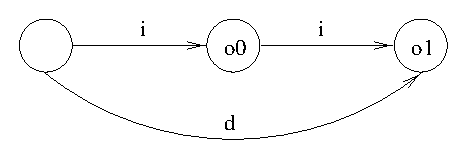
\includegraphics{figures/callfsaeg.eps}}
\centerfigend{fig-callfsaeg}{Sample FSA to Place Integer and Double 
	Floating Point Arguments on Registers}

Given the inadequacy of CCL for out task, we have developed two
new specification languages to support our analysis. The first,
IPL\footnote{\it Keep those acronyms coming!!} (instruction
pattern language) supports the specification of the instruction
sequences from which the caller and callee prologues and epilogues
are composed. IPL is an extension of SLED~\cite{Rams94b}, a language
to support descriptions of machine instruction syntax. IPL extends
SLED to provide support for regular expressions to the language where
the atoms of an expression are individual instructions. The second
language we have developed is PAL (procedure abstraction language).
which provides a means for specifying the calling convention and
other procedure aspects of object code as specified in an ABI.

The following sections demonstrate the use of these
specification languages for the SPARC and Intel platforms. More
detailed descriptions of the languages are given in the \uqbt\ 
source code. 


\section*{SPARC}

The standard stack frame for a single SPARC procedure is composed
of (from low to high addresses) a 16-word area to save the register
window, one word to put the address of a struct/union to return by a
callee, 6 words for a callee to save the first 6 arguments (passed
in registers) to the stack, $n$ words for output arguments 7 and
above, and an area to store locals.  Figure~\ref{fig-stkfrmSparc}
shows the standard stack frame for SPARC.

\centerfigbegin
\resizebox{8cm}{!}{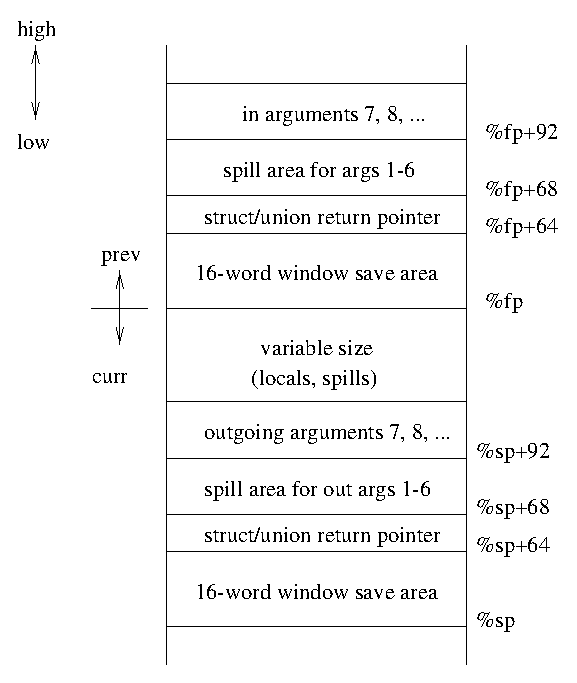
\includegraphics{figures/stkfrm-sparc.eps}}
\centerfigend{fig-stkfrmSparc}{Standard Stack Frame for SPARC Code.
The indexes and register's are given from the context of the callee.}


\subsection{Prologues and Epilogues}

Prior to specifying the prologues and epilogues, it is convenient
to introduce symbolic names for register encodings\footnote{This
is analogous to the {\tt names} construct in SLED.}. For example,
the symbolic name for register 24 on SPARC is {\tt \%o0}. The
set of names defined for SPARC are shown below.

\begin{verbatim}
NAMES
    SP = 14
    FP = 30
    o0 = 8
    i0 = 24
    i7 = 31
    o7 = 15
    g0 = 0
\end{verbatim}

On the SPARC, there are two different ways of invoking a function
based on the return type of the function.  A \texttt{call}
instruction is always used. If the return value is a structure,
union or a quad floating point value, the instruction following the
delayed instruction of the \texttt{call} needs to be a \texttt{unimp}
instruction.  The immediate 22 bits of the \texttt{unimp} are used
to specify the size of the returned value\footnote{Not all compilers
(e.g. gcc) make use of this information to generate runtime size
checking code.}.

\begin{verbatim}
PATTERNS
    CALLER_PROLOGUE std_call addr IS
        call__ (addr)

    CALLER_PROLOGUE struct_call addr IS
        call__ (addr); 
        <4>;  # any 4 byte instruction
        UNIMP (imm22)
\end{verbatim}

The callee prologues that have been identified to date are shown
below. The first two are used when the size of the stack to be
allocated fits into a 13 bit immediate operand. The first one effects
a change to the register window (i.e. allocates a new set of {\it
local} and {\it out} registers) where as the second doesn't. The last
two are analogs of the first two and handle procedures that allocate
a stack whose size cannot be stored in a 13 bit number. A procedure
may not have a prologue at all, as in the case of a leaf procedure
(see page 198 of~\cite{Sparc8}) that doesn't require any stack space.

{\it Note: The last two patterns shown here cannot be used yet as
the pattern parser cannot handle equations or local variables. See
\S\ref{sec:future_work} for a complete description of what is yet
to be implemented to support procedure recovery.}

\begin{verbatim}
    CALLEE_PROLOGUE new_reg_win locals IS
        SAVE ($SP, imode(locals), $SP)

    CALLEE_PROLOGUE same_reg_win locals IS
        ADD ($SP, imode(locals), $SP)

    CALLEE_PROLOGUE new_reg_win_large locals { locals = hiVal+lowVal } IS
        sethi(hiVal,reg);
        ADD (reg, imode(lowVal), reg);
        SAVE ($SP, rmode(reg), $SP)

    CALLEE_PROLOGUE same_reg_win_large locals { locals = hiVal+lowVal } IS
        sethi(hiVal,reg);
        ADD (reg, imode(lowVal), reg);
        SAVE ($SP, rmode(reg), $SP)
\end{verbatim}

The callee epilogue for a procedure on SPARC depends on the following
factors:

\begin{itemize}
\item Does it return an aggregate value?
\item Is it a leaf procedure?
\item Is the value to be returned (if any) already in the right
      location?
\item Has it allocated its own stack?
\end{itemize}

While most combinations of these factors are legal, the majority
of programs will only use a limited subset of the possibile
combinations.  The most common represents a standard return from
a non-leaf procedure (and hence resets the register window). The
value to be returned is already in the expected location ({\tt \%o0}
in this case). The alternatives for the first instruction (i.e. the
actual transfer of control) represent the cases of a scalar (or void)
return value and an aggregate return value respectively.

\begin{verbatim}
    CALLEE_EPILOGUE std_ret IS
        [ ret() |
          JMPL (dispA ($i7, 12), $g0) ];
        restore_()
\end{verbatim}

Two other common combinations are similar to the above except the
value to be returned is moved into the expected location by the
{\tt restore} instruction.

\begin{verbatim}
    CALLEE_EPILOGUE ret_reg_val rs1, rs2 IS
        [ ret() |
          JMPL (dispA ($i7, 12), $g0) ];
        RESTORE (rs1, rmode(rs2), $o0)

    CALLEE_EPILOGUE ret_imm_val rs1, imm IS
        ret();
        RESTORE (rs1, imode(imm), $o0)
\end{verbatim}

Lastly, a leaf procedure usually returns with a {\tt retl}
instruction when returning a void or scalar value or a {\tt jmpl}
instruction when returning an aggregate value. The extra offset from
the calling address in the latter case is to skip the {\tt unimp}
instruction discussed previously.

\begin{verbatim}
    CALLEE_EPILOGUE leaf_ret IS
        [ retl() |
          JMPL (dispA ($o7, 12), $g0) ];
        { SUB ($SP, imode(?), $SP) }
\end{verbatim}

Once the callee returns, any return values are in the right place
and the stack has been restored, so there is no caller epilogue.

The prologues and epilogues presented in this section are the basis
for the PAL specification. The PAL specification encapsulates the
information present in the ABI that describes how parameters are
passed and values returned, where locals are stored and any other
architecture specific information. The following sections present the
sections of the PAL specification for SPARC ABI compliant programs.

\subsection{Frame Abstraction}

To simplify a PAL specification, the first section specifies how to
abstract frame and stack relative address by converting them to be in
terms of a single fixed point, the abstract frame pointer (AFP or
{\tt \%afp}).  Typically, this point should be the value of the stack
pointer after the callee prologue (if any) has been effected as this
is when the abstraction specified takes place. On SPARC, {\tt \%afp}
is indeed initialised to the stack pointer (i.e. {\tt \%sp}). The
substitutions to convert other frame and stack relative addresses to
{\tt \%afp} relative addresses is specified in terms of the callee
prologues previously specified. The only two\footnote{Well four, if
you consider the prologues we can't yet handle.} callee prologues on
SPARC are similar enough that the same substitution for the frame
pointer (i.e. {\tt \%fp}) can be used.  The analysis tracks any
changes to either {\tt \%sp} or {\tt \%fp} throughout the procedure
and updates their respective substitutions correspondingly.

\begin{verbatim}
FRAME ABSTRACTION
    INIT = %sp
    new_reg_win
    same_reg_win
    {
        %fp -> %afp - locals
    }
\end{verbatim}


\subsection{Local Variables}
Local variables are stored within a procedure's stack frame. The size
of this stack frame can be derived from a callee prologue (\textit{We
are assuming that this is always true}). The example below states
that on SPARC, the amount of space (in bytes) allocated for local
variables is equal to the value of the {\tt locals} parameter of
the {\tt new\_reg\_win} and {\tt same\_reg\_win} callee epilogues.

\begin{verbatim}
LOCALS
    new_reg_win
    same_reg_win
    {
        locals
    }
\end{verbatim}

{\it Ideally, we would like to recognise any access addresses within
the portion of the stack frame used for local variables. However,
given the problem of aliasing this is non-trivial and requires
extensive analysis. Even with such analysis, there is no guarantee
that all such references will be detected. The approach we take is
simpler and completely reliable. The user specifies how to derive
the size of the block of memory allocated for locals from the callee
prologue\footnote{I am assuming that this will always be possible}.}

\subsection{Parameter Locations}

As discussed in \S\ref{sec-callConvSpec}, at the machine-code
level we cannot distinguish the variables and types that were used
when placing parameters on appropriate parameter-passing locations.
On SPARC, all parameters are copied by instances of one word, hence,
a double floating point value is copied as two words, in exactly
the same way as two individual integers or even two addresses are
copied.  Low-level type information can be retrieved from usage at
the called site.

The ABI specifies which locations are used for passing parameters,
and the order of usage of those locations. The means by which
the parameters are referenced across a call boundary is dependent
upon the {\it view change} effected by a call. The view change can
be thought of as the low level analog of using actual and formal
parameters in source code. That is, the same parameter is referenced
differently depending on whether the context of the reference is
the call instruction or in the called procedure.

To account for the view change effected by a call, we specify
parameter locations from the both context of the caller (outgoing
parameters) and the callee (incoming parameters).

The first part of the parameters section specifies where the outgoing
parameters are found. This is acheived by attaching a parameters
specification to the {\tt CALLER} keyword.

\begin{verbatim}
PARAMETERS
    CALLER
    {
        AGGREGATE -> m[%afp + 64]
        REGISTERS -> %o0 %o1 %o2 %o3 %o4 %o5
        STACK     -> BASE = [%afp + 92]
                     OFFSET = 4
    }
\end{verbatim}

Each sub-clause is optional but if present, it must obey the
ordering implied in the above example (i.e. {\tt AGGREGATE} before
{\tt REGISTERS} before {\tt STACK}). This ordering complies with
how parameters are passed on all architectures we have encountered.

The \texttt{AGGREGATE} sub-clause states where the address of an
aggregate value to be returned is found. This location will only
be used by calls to procedures that actually return a struct.
Additionally, only some architectures (such as SPARC) make use of
a special location for this purpose. Others (e.g. Intel) simply
pass it as the first parameter\footnote{This effectively makes it a
``hidden" argument in that it doesn't correspond to any source code
level parameter.}.

The {\tt REGISTERS} sub-clause states that registers {\tt \%o0..\%o5}
(in that order) are used for the first 6 parameters (after the
aggregate address parameter if used). Any extra parameters are
passed via the stack and are found in locations {\tt m[\%afp + 92],
m[\%afp + 96], m[\%afp + 100], ...} as specified by the {\tt STACK}
subclause.

In addition, there can be an {\tt ALIGNMENT} sub-clause, after the
{\tt STACK} and before the closing curly bracket. {\tt REGISTERS}
can also have a
type before it, to designate the type of parameters that the given
registers can hold. The type can be one of {\tt INTEGER}, {\tt FLOAT},
or {\tt DOUBLE}. Where a type is not given, as above, {\tt INTEGER} is
assumed. Where more than one type of register is given, they must be
in the order {\tt INTEGER}, {\tt FLOAT}, then {\tt DOUBLE} (with any or
all being optional). For example, for HP pa-risc:

\begin{verbatim}
PARAMETERS
    CALLER
    {
        AGGREGATE -> m[%r28]
        INTEGER REGISTERS -> %r26 %r25 %r24 %r23
        FLOAT   REGISTERS -> %fr4 %fr5 %fr6 %fr7
        DOUBLE  REGISTERS -> %fd5 %fd7
        STACK -> BASE = [%afp - 52]
                 OFFSET = -4
        DOUBLE ALIGNMENT 8 BYTES
    }

\end{verbatim}

When multiple {\tt REGISTERS} are given as above, they are considered to
operate ``in parallel". In other words, when the first parameter goes into
either \%r26 or \%fr4, this ``parameter slot" is ``used up", and so the next
parameter goes into register \%r25, \%fr5, or \%fd7, depending on the type.
If the first parameter is a {\tt DOUBLE}, then two parameter slots are
used up.

The {\tt ALIGNMENT} sub-clause states that parameters of type {\tt DOUBLE}
(64 bit floating point) are aligned on 8 byte boundaries. This applies to
registers and stack locations alike; that's why there are only two
{\tt DOUBLE REGISTERS}. As an example, if a pa-risc function took an
integer, a double, and an integer, then even though these could easily
fit into three registers, they are actually placed in registers \%r26,
\%fd7, and stack location [\%afp-52]. The alignment of the double parameter
``skips" register \%r25, and because doubles are twice as big as integers,
using \%fd7 ``uses up" the parameter slots for \%r24 and \%r23. So the third
parameter has to go to the stack. If there was a fourth parameter of type
{\tt DOUBLE}, it would go to [\%afp-64] (and the other half at [\%afp-60]),
skipping the word at [\%afp-56] to keep the argument aligned on 8 byte
boundaries.

This indicates a significant difference between SPARC and pa-risc architectures.
On the non aligned SPARC, a {\tt DOUBLE} parameter could be split between
an integer register and the stack. On the aligned pa-risc, such splits
can't happen. On the other hand, ``gaps'' in the parameters can be seen
in pa-risc programs, while these will never be seen on the SPARC.

Outgoing parameters are always placed at the same locations. Incoming
parameters however, depend upon the prologue of the procedure being
invoked as it is this prologue that effects the aforementioned
view change. Stack parameters may be found at different offsets
after allocation of the procedure's stack frame. Also, a register
window change will mean that some registers will now accessed via
different register names.

On SPARC, the {\tt new\_reg\_win} prologue changes the register
window, effectively renaming the eight output registers ({\tt
\%o0..\%o7}) to the eight input registers ({\tt \%i0..\%i7}).

\begin{verbatim}
    new_reg_win
    {
        AGGREGATE -> m[%afp - locals + 64]
        REGISTERS -> %i0 %i1 %i2 %i3 %i4 %i5
        STACK     -> BASE = [%afp - locals + 92] 
                     OFFSET = 4
    }
\end{verbatim}

The other prologue, {\tt same\_reg\_win}, doesn't change the register
window but changes the stack offsets.

\begin{verbatim}
	same_reg_win
    {
        AGGREGATE -> m[%afp - locals + 64]
        REGISTERS -> %o0 %o1 %o2 %o3 %o4 %o5
        STACK     -> BASE = [%afp - locals + 92] 
                     OFFSET = 4
    }
\end{verbatim}

\subsection{Return Locations}

Return values need to be placed in specific registers depending on
the type of the value to be returned. As with incoming parameters,
the locations used will depend on the view change effected by the
prologue of the procedure doing the return.

\begin{verbatim}
RETURNS
    ret_reg_val
    ret_imm_val
    leaf_ret
    CALLER
    {
        INTEGER   IN %o0
        ADDRESS   IN %o0
        FLOAT     IN %f0
        DOUBLE    IN %f0to1
    }
    std_ret
    {
        INTEGER   IN %i0
        ADDRESS   IN %i0
        FLOAT     IN %f0
        DOUBLE    IN %f0to1
    }
\end{verbatim}

Note that double refers to a 64 bit float and as such is returned in
a synthetic register that denotes two 32 bit registers.

Once again, the {\tt CALLER} keyword indicates that the accompanying
specification is from a caller's perspective. In this case it is
where a caller will receive a returned value.

\subsection{Accesses to a Parent's Stack}

This is the first (and so far, only) section that is optional in
that not all architectures will require it.

On SPARC, a procedure may write to a certain portion of its parent's
stack frame. This capability is provided primarily so that parameters
in registers can be spilled to the stack resulting in all parameters
being located in a contiguous segment of memory. This is typically
required when the source code uses variable argument lists or
takes the address of a parameter. Compiler writers can leverage
this capability and use this portion of the parent's stack as
space for temporary variables. In order to abstract away from
referring stack locations, we replace accesses to these addresses
with variables. To do so requires that these addresses are specified
in a PAL specification as shown below.

\begin{verbatim}
PARENT STACK
    new_reg_win
    same_reg_win
    {
        %afp - locals + 68 TO %afp - locals + 88 STEP 4
    }
\end{verbatim}

\section*{Intel}

The standard stack frame of a procedure includes space for arguments,
the return address of the caller, the frame pointer value of the
caller (\texttt{\%ebp}), and enough space for local variables and
spilled values (including registers that need to be preserved across
procedure calls).  Figure~\ref{fig-stkfrmIntel} shows the standard
stack frame for Intel code.

\centerfigbegin
\resizebox{10cm}{!}{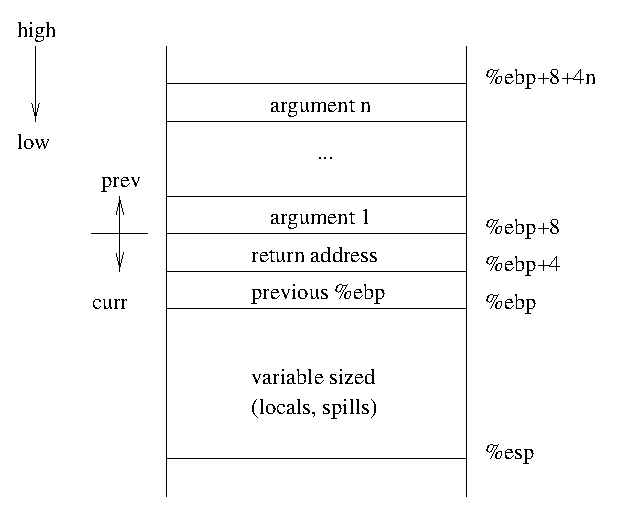
\includegraphics{figures/stkfrm-intel.eps}}
\centerfigend{fig-stkfrmIntel}{Standard Stack Frame for Intel Code}

\subsection{Prologues and Epilogues}

As with SPARC, we start the prologue and epilogue specification by
declaring symbolic names for the register encodings.

\begin{verbatim}
NAMES
    EAX = 0
    ECX = 1
    EDX = 2
    EBX = 3
    ESP = 4
    EBP = 5
    ESI = 6
    EDI = 7
\end{verbatim}

On Intel x86, there is only one way to invoke a procedure, even if
the procedure is to return a value or a structure.  The \texttt{call}
instruction is used, and although this assembly instruction maps to
one of five different machine instructions, only one is used for
direct calls; the intra-segment direct call {\tt CALL\_.JVOD}.  For
indirect calls (i.e. via a register), the intra-segment indirect call
is used (CALL.EVOD modrm).  Indirect calls require extra analysis to
determine the target address of the call; this is addressed in a
different document.  For now assume all calls are direct.

\begin{verbatim}
PATTERNS
    CALLER_PROLOGUE std_call addr IS
        CALL.Jvod (addr)
\end{verbatim}

The most common callee prologue sets up the frame base pointer and
the stack pointer, as well as optionally allocating space on the
stack for locals and spilled values.  Further, the contents of
registers \texttt{\%edi}, \texttt{\%esi} and \texttt{\%ebx} need to
be preserved across procedure calls.  That is, if these registers are
used by the callee, they need to be spilled to the stack as part of
the prologue. 

\begin{verbatim}
    CALLEE_PROLOGUE std_entry locals=0, regs IS
        PUSHod ($EBP);
        MOVrmod ($EBP, Reg($ESP));
        { SUBiodb (Reg ($ESP), locals) |
          SUBid    (Reg ($ESP), locals) };
        { [ PUSHod ($ESI) |
            PUSHod ($EBX) |
            PUSHod ($EDI) ] *regs <1..3> }
\end{verbatim}

In the case where an aggregate value is to be returned, the address
at which this value is to be stored can be passed as the first
(hidden) argument of the call. It has been noted that some compilers
move this address into {\tt \%eax} as part of the prologue\footnote{
Initially this was believed to be an optimisation as the address of a
returned aggregate value must be in {\tt \%eax} upon returning from
the procedure.  However, analysis shows that this is not the case as
these procedures subsequently write to {\tt \%eax} before doing a
return. It does mean the simple form of {\tt RET} can be used in the
epilogue but I'm not sure that this can be classified as an
optimisation}.

\begin{verbatim}
    CALLEE_PROLOGUE struct_ptr locals, regs IS
        POPod ($EAX);
        XCHG.Ev.Gvod (E (Base ($ESP)), $EAX);
        @std_entry (locals, regs)  
\end{verbatim}

The standard epilogue restores any of the registers that need to be
preserved across a procedure call (i.e. \texttt{\%ebx},
\texttt{\%esi} or \texttt{\%edi}), restores the stack pointer and the
frame pointer, and returns to the caller's return address.  Restoring
registers to be preserved across procedure calls can be done in one
of two ways; by popping them from the stack, or by indexing into the
stack directly.  It has also been noticed that some compilers
generate a \texttt{LEAod} (load effective address) at the start of
the epilogue, to ensure the stack pointer is pointing to the right
address, even if this instruction is redundant (as has been seen in
gcc -O2 generated code). The {\tt RET.Iw} instruction is used to
remove the address of a returned aggregate value if this hasn't
already been done so by the prologue.

\begin{verbatim}
    CALLEE_EPILOGUE std_ret IS
        { LEAod ($ESP, Disp8(?,$EBP)) };
        { [ MOVrmod ($EBX, E( Disp8(?,$EBP))) |
            MOVrmod ($ESI, E( Disp8(?,$EBP))) |
            MOVrmod ($EDI, E( Disp8(?,$EBP))) ] * <1..3>
          |
          [ POPod ($EBX) |
            POPod ($ESI) |
            POPod ($EDI) ] *<1..3> };
        [ LEAVE () | [ MOVrmod ($ESP, Reg($EBP)); POPod ($EBP) ]];
        [ RET () | RET.Iw (?) ]
\end{verbatim}

Simple procedures that use no stack and take no parameters have a
very basic epilogue.

\begin{verbatim}
    CALLEE_EPILOGUE simple_ret IS
        RET () | RET.Iw (?)
\end{verbatim}
 

Upon return from a call, the stack needs to be restored by the caller in 
order to remove the parameters that were passed on the stack.  
Restoring of the stack is done by modifying the value of the stack
pointer by a certain number of bytes, or by popping values from the
stack a certain number of times (4 bytes at a time).  Either way 
will tell us how many bytes are restored from the stack. 

\begin{verbatim}
    CALLER_EPILOGUE clear_stack n IS
        [ ADDiodb (Reg($ESP),n) | ADDid (Reg($ESP),n) ] |
        [ POPod ($EAX) |
          POPod ($EBX) |
          POPod ($ECX) |
          POPod ($EDX) |
          POPod ($ESI) |
          POPod ($EDI) |
          POPod ($EBP) ] * n <1..7>
\end{verbatim}

\subsection{Frame Abstraction}

On Intel, we initialise {\tt \%afp} to be the value of {\tt \%esp}
after the prologue (if any) has been executed. As with SPARC, a
similiar substitution is specified for the frame pointer.

\begin{verbatim}
FRAME ABSTRACTION
    INIT = %esp
    std_entry
    struct_ptr
    {
        %ebp -> %afp + (regs * 4) + locals
    }
\end{verbatim}


\subsection{Local Variables}
The size of the block of memory allocated for local variables will
be the initial increment to the stack pointer plus the number of
bytes pushed to the stack when preserving registers.

\begin{verbatim}
LOCALS
    std_entry
    struct_ptr
   {
      locals + (regs * 4)
   }
\end{verbatim}

\subsection{Parameter Locations}

Outgoing parameters on Intel are always found at the bottom of the
stack. Given that we can't statically specify where the bottom of
the stack is, we simply choose a fixed stack address. Accompanied
with a negative offset, this implies that all address that are at
multiples of this offset from are potential parameter locations. The
analysis will then determine which of these locations are live at a
call and recovery as many as it needs to match the signature of the
callee, starting at the lowest addresses. This is exactly the same
approach taken with stack parameters on SPARC but the fixed point
specified in the SPARC PAL specification just happens to be the lowest
address (as implied by the positive offset accompanying it).

\begin{verbatim}
PARAMETERS
    CALLER
    {
        STACK     -> BASE = [%afp - 4]
                     OFFSET = -4
    }
\end{verbatim}

Procedures with the {\tt std\_entry} prologue will find their incoming
parameters at positive offset from the frame pointer. Of course, the
specification is given in terms of {\tt \%afp} as we want to abstract
away from concepts such as a frame pointer.

\begin{verbatim}
    std_entry
    {
        STACK     -> BASE = [%afp + locals + (regs * 4) + 8]
                     OFFSET = 4
    }
\end{verbatim}

The {\tt struct\_ptr} prologue contains the side effect of popping
the address of the aggregate value to be returned from the stack into
{\tt \%eax}\footnote{It it turns out that some other register is used,
then the register used can be parameterised in the pattern and the
parameter name used here instead of {\tt \%eax}.}. As such, the
incoming parameters specification for procedures prefixed with this
prologue require an {\tt AGGREGATE} location to be included.

\begin{verbatim}
    struct_ptr
    {
        AGGREGATE -> %eax
        STACK     -> BASE = [%afp + locals + (regs * 4) + 8]
                     OFFSET = 4
    }
\end{verbatim}

\subsection{Return Locations}

The RETURNS section specifies where returned values can be found. Again,
there are subsections for each callee prologue, and one for callers, using
the special keyword CALLER. Often the different integer values (byte,
short, int) are returned in the same register. If, and only if, the register
numbers are different for the integral subtypes, then an entry should exist
for INTEGER.16 and so on. On a RISC machine like SPARC, parts of registers
are typically not given different register numbers, so these don't appear:

\begin{verbatim}
RETURNS
# Note: even though functions with save/restore return integer locations in %i0,
# we use the STD_RET_ pseudo instruction for these, which copies %i0 to %o0.
# This simulates the semantics of the restore (for the purposes of return
# location), so we don't need a separate set of locations for these functions
    ret_reg_val
    ret_imm_val
    leaf_ret
    std_ret
    CALLER
    {
        INTEGER.32  IN %o0
        ADDRESS     IN %o0
        FLOAT.32    IN %f0
        FLOAT.64    IN %f0to1
    }
\end{verbatim}

On Intel, all fixed point scalar values are returned in {\tt \%eax},
but the word and byte part of eax is called a different register name.
All floating point values are returned on the top of the floating
point stack. The register number of the top of stack depends on whether
a caller or callee is involved:

\begin{verbatim}
RETURNS
    std_ret
    frameless_epi
    {
        INTEGER.32  IN %eax
        INTEGER.16  IN %ax      # So that functions returning shorts
        INTEGER.8   IN %al      # or chars can be analysed as such
        ADDRESS     IN %eax
        FLOAT.80    IN %st7
    }

    CALLER
    {
        INTEGER.32  IN %eax
        INTEGER.16  IN %ax      # So that functions returning shorts
        INTEGER.8   IN %al      # or chars can be analysed as such
        ADDRESS     IN %eax
        FLOAT.80    IN %st
    }
\end{verbatim}

\subsection{Accesses to a Parent's Stack}

Intel procedures never access any stack locations outside of their
own stack apart from those storing incoming parameters.

\section{Procedure Abstraction Analysis}

The goal of this analysis is to use the specification described in the
preceeding sections to remove any references to stack locations in
object code. Such references will be recovered into either parameters
or local variables. There are 5 steps involved in this analysis:

\begin{enumerate}
\item Replace all stack and frame pointer relative addresses with
  their equivalent {\tt \%afp} relative addresses.
\item Recover the signature (parameters only) of user code procedures.
\item Analyse each call to recover the actual parameters of the call.
  this step also includes recovering the return type of the procedure
  called if it isn't a library procedure.
\item Replace any accesses from within a procedure to locations in its
  parent's stack with accesses to local variables.
\end{enumerate}

This analysis is to be performed only on user procedures; library
procedures will be assumed to have been processed by now, either
through generation of call signatures from header files or through
application of the following analysis to library code.

The following subsection consider each of the above steps in
detail. Throughout this section we will make use of the SPARC
example in Figure~\ref{fig-c_gcd}.  Issues specific to Intel are
discussed in $\S$\ref{sec-callsigIntel}.

\centerfigbegin
{\small
\begin{verbatim}
gcd:                           main:
    save %sp,-112,%sp               save %sp,-112,%sp
    mov %i0,%l0                     mov 10,%o0
    cmp %l0,%i1                     mov 5,%o1
    bge .LL12                       sethi %hi(.LLC0),%l0
    mov %i1,%i0                     call gcd  
    b .LL12                         or %l0,%lo(.LLC0),%l0
    mov %l0,%i0                     mov %o0,%o3
.LL6:                               mov %l0,%o0
    call .rem                       mov 10,%o1
    mov %i0,%o1                     call printf  
    cmp %o0,0                       mov 5,%o2
    bne,a .LL12                     ret
    add %i0,-1,%i0                  restore
    mov %i1,%o0
    call .rem  
    mov %i0,%o1
    cmp %o0,0
    be .LL10
    nop
    add %i0,-1,%i0
.LL12:
    cmp %i0,1
    bg .LL6
    mov %l0,%o0
.LL10:
    ret
    restore
.LLC0:
    "gcd of %d, %d is %d\n"
\end{verbatim}
}
\centerfigend{fig-c_gcd}{SPARC Assembly Code for GCD Program}


\subsection{Recovery of Parameters}
Actual parameters are placed by the caller in one or more of the
locations specified by \texttt{caller parameters}.  The callee
will effect the \texttt{view change} applicable to its prologue, 
and will then use the passed parameters directly or place them 
on the parameter spill area.  Either way, the parameters are 
used before definition within the callee, and this is what 
tells us that the information in that location was setup elsewhere
in the program. 

In the example of Figure~\ref{fig-c_gcd}, \texttt{main} calls 
\texttt{gcd}, using the most frequently used calling convention;  
\texttt{interface1}.  
At the \texttt{call} site, the parameter locations that are live are: 
\begin{verbatim}
     live = {%o0, %o1}
\end{verbatim}
At the callee site, we apply the \texttt{view change} of 
\texttt{callee\_prologue1} to the live parameter locations, the 
stack pointer, and the return address, leading to
\begin{verbatim}
     %o0 -> %i0
     %o1 -> %i1
     %sp -> %fp
     %o7 -> %i7
     %sp -> %sp-112
\end{verbatim}
For \texttt{gcd} we summarize the live-in information for the whole 
procedure based on the parameter locations (view changed).  This gives us
\begin{verbatim}
     liveIn(gcd) = {%i0, %i1}
\end{verbatim}
This information tells us that there are 2 parameters, which match the
two live parameter locations at the call site, hence the actual 
parameters to the call are \texttt{\%o0} and \texttt{\%o1}.  The 
transformed CALL instruction looks like this:
\begin{verbatim}
     CALL gcd [<ret type>] <(%o0,<type>), (%o1,<type>)>
\end{verbatim}

Note that for parameter locations that are on the stack, the 
view change of these looks as follows:
\begin{verbatim}
     %sp+92+n -> %fp+92+n
\end{verbatim}
Hence, accesses to \texttt{\%fp+92+n} at the callee site are 
accesses to parameter locations.  It is also feasible for the
callee site to access these locations using the stack pointer; 
this is needed for leaf routines but it can also be used in 
non-leaf routines: 
\begin{verbatim}
     %sp+(92+simm13)+n
\end{verbatim}
We need to support both views of stack parameter locations.


\subsubsection*{Fixed vs Variable Number of Arguments}
Most procedures take a fixed number of arguments.  However, languages
like C allow for variable number of arguments to be passed at any
one time.  The ABI~\cite{Unix90} does not place any rules on variable 
number of parameters, but states that the calling convention rules need to 
be satisfied; that is, the first 6 word parameters go into registers
and the next go onto the stack.  Disassembled C code shows that 
the first thing the callee does is to move all the register parameters
to the parameter spill area, and then use them all on the stack 
(as the stack parameters are contiguous to the spilled register 
parameters). 

It is not clear that in all cases usage analysis of parameter 
locations at the callee will determine the number of parameters
taken by the callee (think of \texttt{printf}, it can take any
number and the code is bound to be a loop on a string).  
Also, different invocations of the procedure will take different
number of arguments.
\emph{I propose we pass all the live parameter locations at the call
site in the mean time; we will see from the implementation whether
this will cause problems with stack parameter locations.}


\subsection{Recovery of Return Value}
The callee will place a return value on a valid \texttt{callee return}
location.  We note that if anything is placed on a return location,
this location will be live-out of the callee.  
The caller will need to apply the inverse of the \texttt{view change}
to live-out callee locations.  
If the caller is to make any use of a returned value, the location
where it was stored will be used before being re-defined.  Usage is 
commonly in the form of storing to a local variable or using it
as a parameter to another procedure.  
Once this is determined, the callee's RET instruction is set to 
return the relevant return location.
 
For the example of Figure~\ref{fig-c_gcd}, the callee, \texttt{gcd}, 
has only one return location live-out, which matches its \texttt{callee
return} for \texttt{interface1}: 
\begin{verbatim}
     live-out = {%i0}
\end{verbatim}
The caller uses \texttt{\%o0} before definition, hence this is our
return location. 
The callee's RET instruction can now be transformed to: 
\begin{verbatim}
    RET %i0
\end{verbatim}
The caller's CALL instruction can now be transformed into an ASSIGN 
(assignment) instruction as follows: 
\begin{verbatim}
    %o0 = CALL gcd <(%o0,<type>), (%o1,<type>)>
\end{verbatim}

\emph{Should we introduce a HL ASSIGN or shall we use RTL assign 
instead?}

Note that as of 8th September 2000, the return value analysis is done before
the actual parameter analysis. This is because the return value analysis
may cause re-analysis of some of the children, which may impact on the
parameters of the call being considered.

\subsubsection*{Returned Values not Used}
Returned function values are not always used by the caller.  In such
cases, different invocations of the same procedure will show different
return location usage.  In these cases, we go for the more general 
one (i.e. the procedure returns a value) and we annotate each actual 
call with whether the return value is used or not.  In this way, the
signature for the procedure is correct. 


\subsection{Issues Relating to Intel Call Signature Analysis}
\label{sec-callsigIntel}
The nature of Intel passing parameters on the stack means that
optimizing compilers may delay the restoring of the stack until 
after several calls to (different) procedures have been emitted. 
This means that the caller epilogue is optional, and where 
available, it may not necessarily match the number of bytes 
passed as parameters to the caller but may also include bytes
used in a previous call.  We can still make use of liveness 
analysis to determine which arguments are passed to each procedure 
nevertheless.
For the purposes of illustration, we will make use of 
Figure~\ref{fig-gcdIntel}, an optimized version of the GCD program for Intel.

\centerfigbegin
{\small
\begin{verbatim}
gcd:                        main:
    pushl %ebp                  pushl %ebp
    movl %esp,%ebp              movl %esp,%ebp
    pushl %edi                  pushl %esi
    pushl %esi                  pushl %ebx
    pushl %ebx                  movl $10,%esi
    movl 8(%ebp),%ebx           movl $5,%ebx
    movl 12(%ebp),%edi          pushl %ebx
    movl %edi,%esi              pushl %esi
    cmpl %edi,%ebx              call gcd
    jge .L12                    pushl %eax
    movl %ebx,%edi              pushl %ebx
    jmp .L12                    pushl %esi
.L6:                            pushl $.LC0
    movl %ebx,%eax              call printf
    cltd                        leal -8(%ebp),%esp
    idivl %edi                  popl %ebx
    testl %edx,%edx             popl %esi
    jne .L7                     leave
    movl %esi,%eax              ret
    cltd
    idivl %edi
    testl %edx,%edx
    je .L13
.L7:
    decl %edi
.L12:
    cmpl $1,%edi
    jg .L6
.L13:
    movl %edi,%eax
    leal -12(%ebp),%esp
    popl %ebx
    popl %esi
    popl %edi
    leave
    ret  
.LC0:
    "gcd of %d, %d is %d\n"
\end{verbatim}
}
\centerfigend{fig-gcdIntel}{Intel Optimized Assembly Code for GCD Program}

Procedure \texttt{main} calls \texttt{gcd} using the calling convention 
specified in \texttt{interface2} with an immediate value of 12 bytes. 
The calling convention does not include a caller epilogue. 
At the \texttt{call} site, the \emph{parameter locations} that are live are: 
\begin{verbatim}
     live = {[%esp], [%esp+4]}
\end{verbatim}
Applying the \texttt{view change} for \texttt{interface2} to the live
parameter locations we get: 
\begin{verbatim}
     ['%esp]   -> [%esp+20]
     ['%esp+4] -> [%esp+24]
and
     ['%esp]   -> [%ebp+8]
     ['%esp+4] -> [%ebp+12]
\end{verbatim}
Procedure \texttt{gcd} has the following set of parameter locations
live on entry, and return locations live on exit: 
\begin{verbatim}
     liveIn = {[%ebp+8], [%ebp+12]}
     liveOut = {%eax}
\end{verbatim}
The liveIn parameters match the ones that were live on entry, hence 
we can safely assume that 2 words (8 bytes) were passed as arguments.
The call is transformed to the following HL instruction: 
\begin{verbatim}
    CALL gcd [<ret type>] <([%esp],<type>), ([%esp+4],<type>)>
\end{verbatim}
which is further transformed into what was actually placed at those 
stack locations (i.e. this information needs to be stored previously): 
\begin{verbatim}
    CALL gcd [<ret type>] <(%esi,<type>), (%ebx,<type>)>
\end{verbatim}
The liveOut information tells us that \texttt{\%eax} is returned. 
Further, at the caller's site, the value of \texttt{\%eax} is 
used prior to definition.  Even if this value was not used, the ABI 
states that return locations should only be set to a value if they
are intended to return a value, as there is no type checking on 
this interface.  The return instruction in \texttt{gcd} is changed to
\begin{verbatim}
     RET %eax
\end{verbatim}
and the caller's site call is changed to 
\begin{verbatim}
     %eax = CALL gcd <(%esi,<type>), (%ebx,<type>)>
\end{verbatim} 
Although there is no caller epilogue to restore the stack, we have
determined the right arguments to this call.

The next call that \texttt{main} performs is to the library procedure 
\texttt{printf}.  In this case, if we had signatures for \texttt{printf} 
we could only be assured of one fixed parameter (an address) and maybe
some more parameters, as this is a variable argument procedure.  
Also, the calling convention does not specify a caller epilogue in 
this case either, hence we cannot determine exactly how many bytes
are passed on the stack to this call.  The best that can be done is
to pass \emph{all} parameter locations that are live at the call site: 
\begin{verbatim}
     live = {[%esp], [%esp+4], [%esp+8], [%esp+12], [%esp+16], [%esp+20]}
\end{verbatim} 
When replacing this information into the HL call, we get: 
\begin{verbatim}
     CALL printf <(.LC0,<addr>), (%esi,<type>), (%ebx,<type>), (%eax,<type>),
                  (%esi,<type>), (%ebx,<type>)>
\end{verbatim}
Note that in this case, the last two arguments are still technically
live as the stack wasn't restored.  Although we are passing them to 
\texttt{printf}, the code within \texttt{printf} will not use them 
as they were not expected (by checking the string \texttt{.LC0}). 

If however the stack was restored after the call to \texttt{printf}, 
the following code could have been emitted to restore both calls made
by \texttt{main}: 
\begin{verbatim}
     addl $24, %esp
\end{verbatim}
Which would account for 8 bytes that we already know \texttt{gcd} takes
as arguments, and 16 bytes for \texttt{printf}.  This type of arithmetics
will allow us to determine the number of bytes passed to variable 
argument procedures in some cases (bearing in mind that each time 
a different number of arguments may be passed). 


\section{EBNF for the PAL Language}

The EBNF for the PAL language follows.  The standard EBNF
metasymbols are used:

\begin{itemize}
\item \verb!{a b}! for sequence
\item \texttt{[a]} for optional constructs
\item \texttt{(a|b)} for alternative choices
\item \texttt{*} for zero or more occurrences
\item \texttt{+} for one or more occurrences
\end{itemize}

\begin{fnverbatim}
PALSpec ::= register_names
      caller_prologue_section callee_prologue_section
      callee_epilogue_section [ caller_epilogue_section ]
      frame_section local_section parameter_section
      return_section [ parent_section ]

register_names ::= "NAMES" { name '=' number } +

caller_prologue_section ::=
      "CALLER_PROLOGUE" pro_epi_decl +
callee_prologue_section ::=
      "CALLEE_PROLOGUE" pro_epi_decl +
callee_epilogue_section ::=
      "CALLEE_EPILOGUE" pro_epi_decl +
caller_epilogue_section ::=
      "CALLER_EPILOGUE" pro_epi_decl +
pro_epi_decl ::= constructor_list

frame_section ::= "FRAME ABSTRACTION" init_decl
      frame_decl +
init_decl ::= "INIT" reg_name
frame_decl ::= name + '{' reg_name "->" afp_exp '}'

local_section ::= "LOCALS" local_decl +
local_decl ::= names '{' exp '}'

parameter_section ::= "PARAMETERS" param_decl+
param_decl ::= names
      '{' "AGGREGATE ->" "m[" afp_exp ']'
          "REGISTERS ->" reg_name +
          "STACK -> BASE = [" afp_exp ']'
                   "OFFSET =" number '}'

return_section ::= "RETURNS" return_decl +
return_decl ::= names
      '{' "INTEGER IN " reg_name
          "ADDRESS IN" reg_name
          "FLOAT IN" reg_name
          "DOUBLE IN" reg_name '}'

parent_section ::= "PARENT STACK" parent_decl
parent_decl ::= name + '{' afp_exp "TO" afp_exp
      "STEP" number '}'

operands ::= name { "," name } *
constructor ::= name { '(' operands ')' }
constructor_list ::= constructor
      | constructor ';' constructor_list
exp ::= "(" exp ")"
      | exp "+" exp | exp "-" exp
      | exp "*" exp | exp "/" exp
      | reg_id | number | name
afp_exp ::=
      "%afp +" exp | "%afp -" exp
reg_name ::= name | reg_id

names  ::= ( name | "CALLER" ) +
name   ::= [A-Z][A-Z0-9_]*[A-Z0-9]
number ::= [0-9]*
reg_id ::= '%'[A-Za-z][A-Za-z0-9]*
\end{fnverbatim}


\section{Location Sets}

Many of the analyses described in this chapter rely on sets of bits representing
locations. This section gives an overview of the LocationMap and BitSet classes
which implement these.

\subsection{LocationMap class}

There is one LocationMap object (part of the CSR class) for the whole program.
It represents a mapping from the integers to locations of interest to the
translation. For example, in one translation, integer 0 might represent "r[8]",
and in another translation it could represent "m[\%afp+92]". It is convenient
to define sets of bits to represent sets of locations. In these sets, if
but {\it n} is on, that means that the expression represented by integer {\it n}
is in the set. That way, expressions such as

  $live_{in}~ = ~\stackrel{\bigcup}{_{all BBs}} ~UsedUndefined~ \bigcap
  ~~({\rm U} - live_{in}$)

can be implemented in code such as

    {\tt for (}{\it bb = each in-edge}{\tt )} \\
    \indent {\tt liveIn |= bb->useUndefSet \& \~~(bb->liveIn);}

\subsection{BitSet class}

There is a Standard Template Library (STL) template class called
\texttt{bitset}, which implements a fixed-size array of bits. Unfortunately,
since we don't know in advance how many locations a program may have, we want a
class with the same functionality as \texttt{bitset}, but has a variable size
(like a vector of bits).  The \texttt{BitSet} class implements this
functionality, using a \texttt{vector} of unsigned integers to hold 32 bits
at a time. Standard bitwise operators like \& and $|$ are used to implement
set intersection and union respectively.

Objects of class \texttt{BitSet} have a member variable called \texttt{usedBits}
which stores the number of bits in this set.
Bits are numbered from 0 to \texttt{usedBits-1}.
\texttt{BitSet}s sometimes have to represent the universal set.
To do this properly, there is a boolean class member called \texttt{universal},
which represents the bits numbered from \texttt{usedBits} to infinity.
Normally, \texttt{universal} is zero, so that the set is finite, and bits
not stored in the vector are considered zero. However, the member function
\texttt{set()} (the one taking no arguments) sets the single vector element
to all ones, and sets the \texttt{universal} bit as well. All bits of this
set are considered to be one.

It is important to take the \texttt{universal} bit into consideration when
performing operations such as \texttt{operator\&}, \texttt{set({\it n})},
and so on. Two member functions, both with the name \texttt{setUsed},
expand the vector when required (e.g. setting or clearing a bit higher than can
be represented with the vector at its current size, or \texttt{and}ing or
\texttt{or}ing with a bitset larger than can be represented with the vector
at its current size. When the vector is expanded, the newly inserted words
are either set to all zeroes or all ones, depending on the state of the
\texttt{universal} bit.

Extra care must be taken when \texttt{and}ing or
\texttt{or}ing with a set smaller (in terms of vector size) than the current
set. For example, when \texttt{and}ing with a smaller set, those elements of
the vector beyond the size of other operand's vector are effectively being
\texttt{and}ed with a virtual word whose bits are all set to the other
operand's \texttt{universal} bit. Hence these words are cleared if the other
operand's \texttt{universal} bit is zero, or left the same otherwise.


\section{Future Work for Procedure Abstraction Recovery}
\label{sec:future_work}

This section details possible extensions and enhancements that can be
made to the procedural abstraction module within UQBT (Doug, Sep 99).

\subsection{Pattern Language for Prologues and Epilogues}

The proposals in this section include extensions to the pattern
language itself (IPL), improvements to the corresponding parser
and suggestions to enforce constraints on how the patterns are used.

\begin{itemize}
\item Add support for locals. Locals are variables that are not
  parameters and as such don't require definition before use. Locals
  can be used to constrain operands over a number of instructions
  without requiring that a parameter is used. Also can be used in
  equations. The example below from SPARC displays both uses:

\begin{verbatim}
    CALLEE_PROLOGUE new_reg_win_large locals { locals = hiVal+lowVal } IS
        sethi(hiVal,reg);
        ADD (reg, imode(lowVal), reg);
        SAVE ($SP, rmode(reg), $SP)
\end{verbatim}

  In this example, {\tt hiVal}, {\tt lowVal} and {\tt reg} are
  all local variables. The first two are used in the equation
  to set the value of the {\tt locals} parameter. The {\tt reg}
  variable enforces the operands of the same name in each of the
  three instructions to have exactly the same value for the whole
  pattern to be successfully matched.

\item Add support for equations. This enables pattern definitions
  like the one above where the value of an operand is derived from an
  expression involving operands of the constituent instructions. In
  this form, equations are exactly the same as supported by SLED.
  However it may be desirable to given equations a finer grained
  scope than the whole instruction. This would allow pattern
  definitions such as the one below where the value of a parameter
  is derived or explicit depending on which branch of the matching
  expression was taken.

\begin{verbatim}
    CALLEE_PROLOGUE new_reg_win locals IS
        SAVE ($SP, imode(locals), $SP) |
        [ sethi(hiVal,reg);
          ADD (reg, imode(lowVal), reg);
          SAVE ($SP, rmode(reg), $SP)
          { locals = hiVal + lowVal }
        ]
\end{verbatim}

  The primary advantage of this extension is that one epilogue
  can match a greater variety of patterns. However it comes at
  the disadvantage of added complex to both the language and the
  underlying parser. As it is, the parser will have to extend its
  semantic checking for equations to ensure for example that any
  variables used in the right hand side of an assignment are defined
  on every branch of the matching expression (e.g. lowVal and hiVal)

\end{itemize}


\subsection{Local Variables}
The current local variable section in a PAL spec only supports
specification of the size of the stack frame which in turn is
the amount of memory we allocate for local variables. On some
architectures such as SPARC, the stack frame includes space for
other purposes than just storing local variables such as space
for saving the register window in the case of a register window
overflow. We would like to be able to allow the user to
specify the portion of the stack frame that is dedicated to local
variables. One means of doing so is to specify a base address and a
size (similar to a stack parameter specification) as in the following
example for SPARC:

\begin{verbatim}
    LOCALS
        new_reg_win
        same_reg_win
        {
                BASE = %afp
                SIZE = locals
        }
\end{verbatim}

This example says that the locals parameters are located in the
inclusive range {\tt m[\%afp] .. m[\%afp + locals]}. Using such a
specification ensures that the translated program will only allocate
as much space for locals as was allocated in the source program.

{\it As long as only the size of the stack is specified, the local will
always be indexed at offsets from {\tt \%afp}. For this reason, the
size specified must always be the same as the difference between the
frame pointer and its equivalent {\tt \%afp} relative value. This can
be seen to hold in both the SPARC and Intel PAL specs.}


\subsection{Aggregate Types as Parameter and Return Types}
When analysing calls to user code procedures, both the caller
and callee can be coerced into a form that will guarantee the
successful compilation of the generated intermediate C code on
the target platform. This results primarily from the fact that the
underlying exposes the calling convention for passing and return
aggregate values in the intermediate code.

Library procedures that have aggregate types in their signature will
expect the calling convention on the target platform for passing
and returning these types to be used by calls to them. The only
way we can do this in C code is to typecast the blocks of memory
storing the relevant aggregate values. Consider a call to the
library function with the following signature:

\begin{verbatim}
    time_t time(time_t *t);
\end{verbatim}

To ensure that the code generated by a call to this function
will be ABI compliant with the library on the target platform, the
intermediate C code must use the {\tt time\_t} name as follows:

\begin{verbatim}
    (*(time_t*)(_t) = time(_t);
\end{verbatim}

where {\tt \_t} is a pointer to the block of memory that will store
the {\tt time\_t} struct. There is no need to typecast the parameter
to the call as type clashes between pointer types will result in
compiler warnings but the correct code will be generated. A typecast 
would have been necessary for the parameter if it was not a pointer type.

At the moment, the analysis does not have access to the type names
required for doing the typecasting described above.

\subsection{Implementation}

This sections describes what is left to be done in the implementation
is general apart from the changes suggested in the preceeding
sections.

\begin{itemize}
\item Change all "csr" substring "pal" to reflect that CSR module is
now the PAL module. This includes changes to directory names, files
names, class names, variables name comments etc.
\end{itemize}

         % procedure abstraction recovery

 	%
% 25 Oct 01 - Brian: Added description of endianness analysis during
%              type analysis.
%

\chapter{Type Recovery Analysis}
\label{ch-type}

\newtheorem{typerule}{Type Rule}[chapter]

{\small
\begin{flushright}
Design: Cristina [Mar 99], Implementation: Mike Van Emmerik[c.00], Bernard Wong [Aug 01], Documentation: Cristina [99], Bernard [Aug 01], Brian [Oct 01]
\end{flushright}
}

{\em The bulk of this document was written in 1999 and has not 
been updated much since.  In summer 2001, Bernard implemented some 
of the type propagation ideas presented in this chapter, 
however, the implementation is not fully tested at the 
time of release of this code.} 

Low-level type recovery is the process of recoverying types 
that are available at the machine level in order for 
translated programs to be correct.  
Type recovery is done in a series of steps, by first annotating
locations with their plausible type and then propagating 
types across live ranges of locations.  

This document will grow as we learn more about the type 
requirements for translated programs.  The following are 
the issues that will be addressed throughout this process: 
\begin{itemize}
\item What is the minimal set of low-level types required?
\item How do we best propagate information across procedures?
\item What information do we need to store for byte swapping 
	to work correctly across different endianness machines?
\end{itemize}

In reality, we are mainly interested in determining the low-level 
types for parameters and return values, however, in order to 
do that, one needs to also know the types for other locations 
that define the variables that get passed as parameters. 
This analysis will be done in the following stages: 
\begin{itemize}
\item Recovery of types for registers
\item Recovery of types for local and parameter locations that 
	are not registers 
\item Recovery of types for other memory locations
\end{itemize}

The second stage involves extending the register analysis to 
support local variable locations as well as parameter locations. 
It may be that parameter locations are trivially supported by
the register analysis (once parameters have been determined), 
and so this stage would be involved with the support of 
local procedure memory.

The last stage is an optional one and is there in case we end 
up doing endianness analysis and attempt to minimize the number
of swaps to memory.  

Unless otherwise seen to be needed later, we will work with 
four base low-level types: integer, float, address to data 
and address to instruction.  
Given that the ABI~\cite{Unix90} states that floats and 
integers (of any size) are passed on integer registers, and the  
fact that addresses are also integer numbers, our default data type
for any location is an integer (i.e. the bottom of the lattice).  
In a lattice representation, if a condition holds true, a type can 
be promoted to one higher up the lattice.  In our case, we have a 
few types which can be represented in a very simple lattice as per 
Figure~\ref{fig-typeLattice}. 

\centerfigbegin
%\resizebox{6cm}{!}
{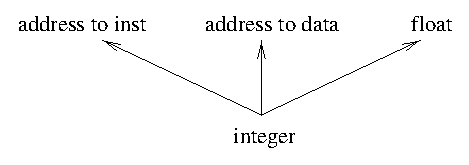
\includegraphics{figures/typeLattice.eps}}
\centerfigend{fig-typeLattice}{Lattice of Low-Level Types} 

Types are determined based on usage of a location across a live
range.  Given that a particular location can be re-used as 
different variables of different types by a compiler, the only
safe assumption is that the live range for a given location will 
have \emph{one} type.  {\emph{I believe this assumption is 
valid for non-overlapping registers.}} 

For the promotion of types, we use a slightly different lattice
to the one displayed in Figure~\ref{fig-typeLattice}.  Distinguishing
integers from addresses is a hard to solve problem as the assembly 
of the machine does not provide for mnemonic instructions to 
distinguish them.  For example, the following code: 
\begin{verbatim}
    sethi %hi(71167),%o1
    or %o1,%lo(71167),%o0
\end{verbatim}
sets register \texttt{\%o0} to the value of \texttt{71167}.  From 
looking at this code alone we cannot tell whether 71167 represents
an address (in the instruction or data area) or a large constant 
number.  Only usage of register \texttt{\%o0} will determine 
the type of 71167.  
For this reason we use the lattice in Figure~\ref{fig-promotionLattice} 
to describe the types of addresses; namely, an integer may ``look like'' 
and address, but until we can identify usage of that integer or 
address, we cannot determine whether it is an address (and hence 
promote to type address). 

\centerfigbegin
\resizebox{6cm}{!}{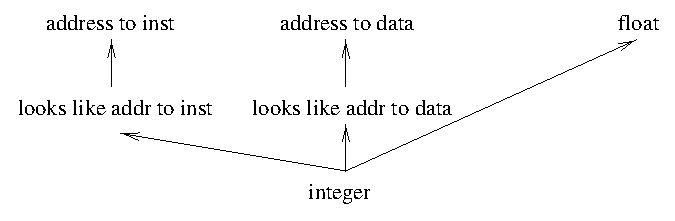
\includegraphics{figures/promotionLattice.eps}}
\centerfigend{fig-promotionLattice}{Lattice of Low-Level Types}

Once a type is determined, types are propagated across the live range 
of the particular location.

Note that even though we place data at the same memory locations
in the target address space as in the source address space, we 
still need to collect type information on pointers to data, as 
this information is needed in getting byte swapping (i.e. the 
simple endianness solution) to work correctly on translated 
programs.


\section{Type Analysis for Registers}
By default, a register is considered to be an integer 
register.  Usage of a register on a procedure call or 
as the return value of a call can change its type.  
Types are propagated from usage to definitions, so here are 
the steps to follow at different parts of the translation 
process: 

\begin{itemize}
\item Collect plausible type information at decoding time.
\item Perform type propagation by type induction.
\end{itemize}


\subsection{Collecting Type Information at Decode Time}
There are three rules that can be used at decoding time 
to annotate type information in registers.  

The first two rules deal with static checking of literal 
constants against addresses of text and data sections, and 
annotating the relevant register to ``looks like'' an address, 
denoted, ``\verb!~!pi'' for looks like a pointer to an instruction, 
and ``\verb!~!pd'' for looks like a pointer to data.  

\begin{typerule}
If a M$_S$-RTL instruction is of the form ``r = Num'' and 
$Num \in$ addrRanges(textSegments), then type(r) = \verb!~!pi.
\label{rule-llpi}
\end{typerule}

\begin{typerule}
If a M$_S$-RTL instruction is of the form ``r = Num'' and 
$Num \in$ addrRanges(dataSegments), then type(r) = \verb!~!pd.
\label{rule-llpd}
\end{typerule}

The following rule applies to any control transfer instruction, 
namely, calls, conditional and unconditional jumps. 
If the target address of the control transfer instruction is 
stored in a register, than that register has pointer to 
instruction type, denoted ``pi''. 

\begin{typerule}
If an M$_S$-RTL instruction is of the form ``controlTransfer r'', then 
type(r) = pi. 
\label{rule-pi}
\end{typerule}


\subsection{Determining Live Ranges of Registers}
In order to propagate types across registers and across 
procedures, live ranges for each register need to be found
first.  A register may take several different variables 
throughout the lifetime of a procedure, hence the need for 
such live ranges. 

A live range extends between the definition (i.e. assignment)
of a register until the death (i.e. re-assignment) of that register.
For example, in the following \texttt{main} code:
\begin{verbatim}
2    mov 10,%o0
3    mov 5,%o1
4    sethi %hi(.LLC0),%l0
5    call gcd
6    or %l0,%lo(.LLC0),%l0
7    mov %o0,%o3
8    mov %l0,%o0
9    mov 10,%o1
10   call printf
11   mov 5,%o2
12   ret
\end{verbatim}

The live ranges for register \texttt{\%o0} are: 
\begin{itemize}
\item Register \texttt{\%o0} becomes live at instruction 2,
    and its live range extends to instruction 5
\item instructions 5 to 8
\item instructions 8 to 10
\item instructions 10 to 12
\end{itemize}


\subsection{Propagating Type Information}
Type propagation can only be performed in \hrtl\ code, i.e. 
after parameter analysis recovery has been performed and 
the program's code has been lifted to the level of machine 
independent RTLs. 

Known types (i.e. non integer) are propagated across live 
ranges of registers, including across procedure calls, 
taking into consideration the signatures for library 
functions.

The first rule states how to go up the lattice when the type 
of the RHS is non integer, basically, propagate from the type of 
the usage to the type of the definition.

\begin{typerule}
If a \hrtl\ instruction is of the form ``r = exp'' and type(exp) = A 
and type(r) = int, then type(r) = A. 
\label{rule-prop-usageDef}
\end{typerule}
 
Note that the type of an expression is the type further up the
lattice of the individual registers forming the expression. 

The next rule looks at the return value of a function call 
and propagates that type to the newly defined register. 

\begin{typerule}
If a \hrtl\ instruction is of the form ``r = call X'' and 
returnType(X) = A, then type(r) = A. 
\label{rule-prop-retValue}
\end{typerule}

The next rule states that a library function's formal argument 
types are propagated to the associated actual parameters.  
In the case of variable argument functions, only the fixed 
formal parameter types can be propagated. 

\begin{typerule}
If a \hrtl\ instruction is of the form ``call libFunc(..., $r_i$, ...)'' 
and the function libFunc has the signature ``libFunc(..., $f_i$=$t_i$, ...), 
then type($r_i$) = $t_i$.  
\label{rule-prop-libFunc}
\end{typerule}
 
The above three rules can be applied on a pass through the code, 
without need of any extra data structures other than the live 
ranges for registers.  The next rule requires extra analysis to 
be performed on procedures, as a register that appears as 
pointing to an instruction may actually be invoked elsewhere in
the program, such as in the \texttt{qsort} program.  

\begin{typerule}
If there is an instruction of the form ``call r''and $\exists$ r2: 
type(r2) = \verb!~! pi, then, if r2 \ra* r, type(r2) = pi. 
\label{rule-reach}
\end{typerule}

In order to apply type rule~\ref{rule-reach}, we need to compute
the reaching definitions of $r2$ throughout the program, including
its transitive closure as the register could have been passed 
as parameter and then copied to another register before it is 
invoked. 


\section{Type Analysis for Other Memory Locations}
Type analysis of other memory locations
can be done to support endianness analysis:
the identification of when endianness swaps are necessary
when the target machine has a different endianness than the source machine.
A translated program's initialized memory is left as-is,
in the source machine's endianness.
We currently swap the bytes of \emph{every} multibyte value
that is read or written to memory.
If type analysis were extended
to include information about the endianness of each value,
then we could determine not only which endianness swaps are unnecessary,
but also when they must \emph{not} be done.
For example, the procedure \texttt{scanf}
is passed an address where its result must be stored.
The value that will be stored in memory
will be in native (target) endianness.
However, when the caller reads the value,
if its bytes are swapped, the native value will be corrupted.
This problem occurs today with every ``call-by-reference'' procedure
that takes addresses where their results are written.

We could do a data flow analysis to discover what values
have native endianness and what do not.
This could be done during type analysis
and a bit set indicating the endianness of each value and location.

Note that it is not enough to specify ``call-by-reference'' information
for just library procedures such as \texttt{scanf}.
The translated program's own procedures
may also be ``call-by-reference''. 


\section{Speculative Decoding}
Trees of program code can be built through speculative 
decoding, in such a way that a forest of trees is built, 
with the main tree being the one that starts at the 
program's entry point.  
Speculative decoding is useful if code ever gets code 
through the interpreter, in which case, the interpreter's 
switch manager can determine if the target address has
already been decoded, in which case, efficient translated
code is run instead of being interpreted.  However, 
speculative decoding is expensive on time resources, 
but for static translators this may be ok anyway.  
 
Type rule~\ref{rule-prologue} states that for all word-aligned
values of $N$ that belong to any of the text segments, if 
the first bytes of that address match a callee prologue (see  
Chapter~\ref{ch-call}, \S\ref{sec-callConvSpec} for SPARC and Pentium 
callee prologues), then $N$ is the start address of a new 
code tree.  

\begin{typerule}
$\forall N: N$ is word-aligned and $N \in addrRanges(textSegments)$ 
and $m[N] \ldots m[N+i]$ = callee\_prologue then type($L$) = $pi$.
\label{rule-prologue}
\end{typerule}

Clearly, applying this technique would be done after the 
normal decoding process and \uqbt\ should have tagged which 
word-aligned memory locations have already been processed 
so that those locations are ignored in this lengthy pass. 


\iffalse
\section{Promotion to Address to Data}
Addresses to data point to data locations in the program, such as
constant data (for example, strings that appeared in the original 
program), and global read and write data. 

An address is an integral number that happens to be a virtual address 
within the range of addresses of the data segment(s) of the program or of 
a symbolic name. 
In Elf binary-files, there are several sections that contain data; 
these are: 
\begin{itemize}
\item Sections that contain read-only data: .rodata, .rodata1
\item Sections that contain initialized read-write data: .data, .data1
\item Section of uninitialized read-write data: .bss
\end{itemize}
Each of these sections has identifying information to know the 
section name, its virtual address and its size.
This data provides us with information that can be used in 
determining whether an integer is an address to data or not. 

The following rules are used to promote integers to addresses to data.
We denote ``address to data'' by $addr_d$ and ``looks like address to 
data'' as $ll_{addr_d}$. 

\begin{typerule}
If $m[i]$ then type(i) = $addr_d$
\label{rule-index}
\end{typerule}

Type rule \ref{rule-index} states that any memory access implies an address 
through its index.  This will be the case for both load and store 
instructions.  Further, $i$ may be an expression, in which case 
the registers within it will contain the value of the address. 
For example:
\begin{verbatim}
  %o0 = m[%l0+4] 
\end{verbatim}
implies that \texttt{\%o0+4} is an address, in which case 
\texttt{\%o0} is the register that contains the address.  

\begin{typerule}
If $L_1 = a[L_2]$ then type($L_1) = addr_d$.
\label{rule-addressOf}
\end{typerule}

Type rule \ref{rule-addressOf} states that if the address of a location is 
taken, then the location represents an address to data.  For example,
the following two RTLs illustrate this point:
\begin{verbatim}
  r[24] = a[m[0x804a250]]
  r[24] = a[m[r[29]-8]]
\end{verbatim}

\begin{typerule}
If $L = Num$ and $Num \in$ addrRange(dataSegments) then type($Num) = ll_addr_d$ 
and type($L) = ll_{addr_d}$.
\label{rule-dataSeg}
\end{typerule}

Type rule \ref{rule-dataSeg} states that if an integral constant is within 
the range of the virtual addresses of the data segment(s) of a program (i.e. 
.rodata, .rodata1, .data, .data1 or .bss in an Elf binary-file), then 
both the integral constant and the location to which it is assigned 
looks like an address to data.  

\emph{Is the information in the dynamic symbol table for type STT\_OBJECT 
relevant?  It contains the virtual address of such objects.}

As can be seen, the type rules that promote to address to data cannot
always solve the problem of accessing data addresses.  However, in 
our implementation, we \emph{force} the data segment(s) of the source 
binary program to be located at the same virtual addresses in the
target program.  Hence, determining whether an address points to 
data or not, does not need to be solved using this model; and 
type rules~\ref{rule-index} to \ref{rule-dataSeg} are not used. 


\section{Promotion to Address to Instruction}
An instruction address points to instructions in a program, normally
the start of procedures or entry points into the code of a function. 

An address to an instruction is a virtual address that falls 
within the text section(s) of the program.  For Elf binaries, the
following sections contain instructions: 
\begin{itemize}
\item The program's text section: .text
\item The program's initialization section: .init
\item The program's finalization section: .fini
\item The program's program linkage table: .plt
\end{itemize}
Further, the dynamic symbol table (.dynsym) also contains names of 
dynamic library procedures.  Such names map addresses which are 
found in the PLT section.

The following rules are used to promote integers to addresses to 
instructions.  We denote ``address to instruction'' by $addr_i$ 
and ``looks like an address to instruction'' by $ll_{addr_i}$.

\begin{typerule}
If $Call L$ then type($L$) = $addr_i$.
\label{rule-call}
\end{typerule}

Type rule \ref{rule-call} states that if a call is made to a target 
location, then that location represents an address to an instruction. 
This rule covers both, calls to known addresses and otherwise, 
such as in the following examples: 
\begin{verbatim}
  call 0x10ae4        ; known target address
  call r[10]          ; computed call, unknown statically unless analyzed
\end{verbatim}

\begin{typerule}
If $Jump L$ then type($L$) = $addr_i$.
\label{rule-jump}
\end{typerule}

Type rule \ref{rule-jump} states that the target location of an 
unconditional jump points to an instruction.

\begin{typerule}
If $Jcond L$ then type($L$) = $addr_i$.
\label{rule-jcond}
\end{typerule}

Type rule \ref{rule-jcond} states that the target location of a 
conditional jump is an address to an instruction.

\begin{typerule}
If $L = Num$ and $num \in$ addrRange(textSegments) then 
type($Num$) = $ll_{addr_i}$ and type($L$) = $ll_{addr_i}$.
\label{rule-textSeg}
\end{typerule}

Type rule \ref{rule-textSeg} states that an integral constant looks 
like an address to an instruction if that constant is within the
range of virtual addresses of the text sections of the program. 
In the case of Elf binary-files, the text sections are .text, 
.init, .fini and .plt. 

\begin{typerule}
If type($L$) = $ll_{addr_i}$ and $L$ uniquely reaches $r[i]$ in 
a $Call r[i]$ statement, then type($L$) = $addr_i$.
\label{rule-reach2}
\end{typerule}

Type rule \ref{rule-reach2} states that a reaching definition of a 
location that looks like an address to an instruction is in fact
an address to an instruction, if the statement it reaches is a 
computed call on a register.

\begin{typerule}
If type($L$) = $ll_{addr_i}$ and $m[L] \ldots m[L+n]$ = callee\_prologue
then type($L$) = $addr_i$.
\label{rule-prologue}
\end{typerule}

Type rule \ref{rule-prologue} states that an integral constant that 
looks like an address to instructions can be promoted to an 
address to instruction if the bytes at that memory location and subsequent 
locations match those of a valid callee prologue (see 
\S\ref{sec-callConvSpec} for SPARC and Pentium callee prologues).

Type rule \ref{rule-prologue} creates a forest of code that is decoded
statically, even when the caller of such code cannot be determined
statically.  In the event of dynamic invocation of such code, 
if the code has been translated, the interpreter's switch manager
will check the address translation table and determine that such
code has already been translated, hence giving control to it 
instead of interpreting it. 

By the nature of building the control flow graph while decoding 
machine instructions, we are in essence applying type rules~\ref{rule-call} 
to \ref{rule-jcond}.  

Type rules~\ref{rule-textSeg} promotes a type to ``looks like an 
address''.  If neither type rules~\ref{rule-reach2} or~\ref{rule-prologue} 
applies, then we cannot say that the particular integral constant is an 
address or not.  As it \emph{may} be an address, we will need to 
pass it as an address in order to prevent programs from crashing. 
In the event that it was an integral constant instead of an address, 
we will emit the wrong result.  

\emph{Can we somehow trap this?  If it goes to a library function,
we have the signature in most cases (except varargs), if it goes 
to user code, then we would have translated it, so we could check 
prior to invoking?}
 

\section{Promotion to Float Type}
A float type is determined when placing a location onto a 
floating point register.  Type conversion procedures such as 
\texttt{itof()}, integer to float, not only perform a type 
conversion but also set the live range of the source and 
target registers used; the source register dies and the target
register starts its live range.  The size of a float is determined
based on the usage of the floating point register(s).  For 
example, when a double register is used, then its size is twice 
the word size (64 for SPARC). 

There are two different types of float values, those that are 
constant and those that go into registers.  The constant values
are easy to determine from the RTLs, as a float number is 
represented by \texttt{FloatNum} in the EBNF and an integer 
number as \texttt{Num}.  

Floating point registers are separate to integer registers in our
RTL model, hence any values that pass through floating point 
registers are of type float.  Further, floating point operators 
and procedures (such as sin and cos) also aid in determining how a 
particular register is used.  

The following rules determine the values of type float: 

\begin{typerule}
If $V = FloatNum$ then type(V) = float.
\label{rule-float}
\end{typerule}

Type rule~\ref{rule-float} states that if a value is of the 
RTL type FloatNum, then it is a floating point value.

\begin{typerule}
If $L = FFunction$ then type(L) = float.
\label{rule-floatFunc}
\end{typerule}

Type rule~\ref{rule-floatFunc} states that if a function that
returns a float is used, then the type of the location becomes
a float.
Note that this rule implies that a register may be used to 
hold integer and floating point values at different points in 
time in the program, hence the live range for a register needs 
to be considered carefully. 

\begin{typerule}
If $L = (Exp BinOP Exp)$ and $BinOP \in Farith$ then type(L) = float.
\label{rule-floatOp}
\end{typerule}

Type rule~\ref{rule-floatOp} states that if a floating point arithmetic
operand is used on the right-hand side expression being assigned to 
location $L$, then the result type of the expression is a float and
hence $L$ is of type float.

\fi


\section{Register Live Ranges}
In order to perform some of the promotion analysis, we need to 
keep track of live ranges for all registers used in a procedure. 
The importance of this is that a register may hold values of 
different types at different points in the program, hence we 
cannot just say ``register 5 is of type float'' as it may be
that it is of type integer and then becomes of type float.  
\emph{A suitable data structure to keep track of ranges and 
types is needed.}

\emph{The following example should be on the RTLs rather than
the assembly code, but uqbts is giving the wrong answer}

A live range extends between the definition (i.e. assignment) 
to a register until the dead (i.e. re-assignment) of that register. 
For example, in the following \texttt{main} code from Figure~\ref{fig-c_gcd}: 
\begin{verbatim}
2    mov 10,%o0
3    mov 5,%o1
4    sethi %hi(.LLC0),%l0
5    call gcd  
6    or %l0,%lo(.LLC0),%l0
7    mov %o0,%o3
8    mov %l0,%o0
9    mov 10,%o1
10   call printf  
11   mov 5,%o2
12   ret
\end{verbatim}

By the time the analysis is done, we will have performed the 
prologue/epilogue analysis, hence the first and last instructions 
are not there.  The live ranges for register \texttt{\%o0} are: 
\begin{itemize}
\item Register \texttt{\%o0} becomes live at instruction 2, 
	and its live range extends to instruction 5 
\item instructions 5 to 8 
\item instructions 8 to 10
\item instructions 10 to 12
\end{itemize}


\section{Reaching Definitions}
In order to apply type rule~\ref{rule-reach}, we need to compute 
the reaching definitions of $L$, the transitive closure of 
reaching definitions.  The use of the \texttt{qsort} example 
is ideal in this case, as two levels of indirection are needed 
in order to find the location where a function pointer gets used. 


\section{Type Recovery Analysis Implementation}

{\small
\begin{flushright}
Implementation and documentation: Bernard [Aug 01]
\end{flushright}
}

In order to evaluate the type recovery processes discussed in the previous
sections of this paper, an initial implementation of type recovery
analysis based on this paper has been completed.

This implementation however is only an initial version and does not
implement every rule stated in this paper. The following is a list of 
type rules that the current version of type recovery analysis implements:

\begin{itemize}
\item Type Rule~\ref{rule-pi} "controlTransfer r", then type(r) = pi
\item Type Rule~\ref{rule-prop-usageDef} "r = exp" and type(exp) = A and 
	type(r) = int, then type(r) = A
\item Type Rule~\ref{rule-prop-retValue} "r = call X" and returnType(X) = A 
	then type(r) = A
\item Type Rule~\ref{rule-prop-libFunc} Type propagation between library 
	functions
\end{itemize}

Without rules~\ref{rule-llpi} and \ref{rule-llpd}, it is not possible to 
implement the ``looks like'' types mentioned earlier in this paper.  
Therefore, the different low-level types that are represented are integer, 
address to instruction, address to data and float.

The first necessary step is to infer the plausible type information of each 
register in each of its live ranges. This step is done after the binary
files has been brought up to the HRTL level of abstraction. It is possible
to perform the initial type recover at the machine specific RTL level. However,
important information such as parameters and return value to functions are not 
available at the machine specific RTL level and will need to be added later. 
For simplicity of implementation reason, it was decided that the type recovery 
analysis will begin after the binary file has been bought up to the HRTL level.

The first information that we want to gather from the HRTL is the location
of every use and definition of each register. From this information, we
can build use-definition chains and determine the live ranges of each register.
Since we assume that the type information for a non-overlapping register in a 
particular live range is always the same, therefore each use-definition chain 
would only have one type and can be used as a means to propagate type 
information of each register across instructions. The use-definition chain 
is therefore one of the most important data structure we use for type recover.

To actually infer the type information, the HRTL instructions need to be parsed
for specific cases that uncover the type information. The HRTL instructions are 
stored in a prefix format as a list of integers called semantic strings. The 
simplicity of this prefix format allowed the creation of a parser, specific
to uncovering type information from semantic strings, to be a relatively 
straight forward process. The following is a list of some of the cases
which the parser is looking for:

\begin{itemize}
\item Registers within MemOf tokens. This can be complicated by functions
	and operations following MemOf tokens.
\item Registers following a control transfer token. 
\item Certain binary operator that has implict type information to the registers
	it operates on.
\item Certain function operators, which often has explict type information
	to the registers it operates on.
\end{itemize}

The parser will first find all the registers that are in the semantic string and
determine whether it is a use or definition of the register. It will insert
this information into a use-definition chain data structure. The parser will
also insert into the data structure any type information that it can infer.

Additional, the parser will look for simple register aliasing situations that 
can later be used for type propagation. For example, in the following example, 
register 1 and register 2 are consider aliases in type value. The 
use-definition chains of these two register at this particular point will be 
linked together. Therefore, if more type information was later discovered 
about register 2, the type information of register 1 would also be updated.

\begin{verbatim}
r[1] = r[2]
\end{verbatim}

This stage of type recovery will already uncover a significant amount of type
information. Long use-definition chains will likely have the correct type
information as the many uses of the register would most likely uncover the
type. 

In order to find the complete use-definition chains for every register, the
program must be analyzed in its entireity. Each register must be tracked 
from its first definition to its last use. There are several implementation
problems with tracking a register in that manner. One problem is the difficulty
in tracking a register as the flow of instruction passes a control transfer
instruction. A register can be defined before the control transfer instruction 
and then be used in both the branches. Therefore, the data structure used for 
the use-definition chains must be complex enough to handle this case correctly.
A second problem is the size of the data-structure used to hold the 
use-definition chains. Since the backend of UQBT that performs code generation 
only looks at HRTL code a basic block at a time, it would be much more 
convenient to also have use-definition data structures for each basic block 
instead of a monolithic one for the whole program. 

The approached that was taken in this implemenation was to create use-definition
chains at the basic block level. This was chosen mostly because of its 
simplicity.  The use-definition chains will always be straight lines at the 
basic block level, as there will not be any control transfer instructions. 
Retrieving the information to insert into the data-structure is also a simple 
process as all the information can be found inside each basic block. 
Therefore, the code to generate the data structure is small and modularized 
for different types of basic blocks. However, the main disadvantage to creating
the use-definition chains at the basic block level is that the chains are 
often incomplete. Many chains will only have uses but no definitions and some 
chains will only have definitions but no uses.
Therefore, this data structure does not store the equivalent amount of 
information as the one that covers the complete program. However, the missing 
information can be recovered by performing type propagation across basic 
blocks and across functions.
The type propagation is simply completing incomplete chains across basic 
blocks and functions. 

To implement type propagation across basic blocks, a depth first traversal of 
the basic blocks inside each function is performed. During the depth first 
traversal, a pointer to the parent of each basic block is kept inside the 
basic block's data structure. At each basic block, use-definitions chains that 
have uses but no definitions are found and are made candidates for type 
propagation. Determining which chains are candidates is a very quick task as 
there are only certain places where incomplete chains may be. Incomplete 
chains are always found as the first use-definition chain of each register.
And each chain can only have one definition which, if it exists, is always 
the first element in the chain. Therefore, only $n$ elements needs to be looked 
at for each basic block to determine which chains need to be propagate, where 
$n$ is the number of registers. Next, to find the definition part of the 
chains, the algorthm will traverse up the call graph, using the pointer to 
the parent basic block stored during the traversal. 

Since this traversal follows the flow of normal execution, traversing back up 
the control flow graph should always find the desired register definition. 
However, there are cases where this might not be true because of the 
limitation of keeping only one single pointer to the parent basic block. It 
also depends on the aggressiveness of the traversal.

The original traversal algorithm that was implemented would only consider every
basic block once. Once a particular basic block has been reached, a flag is 
marked to indicate that future traversals should end before reaching this basic
block. However, this traversal is much too conservative as it only consider one
path to each basic block when there could possibly be many paths. To solve this 
problem, a more aggressive traversal algorithm allowed a basic block to be 
traversed multipled times. To avoid infinite loops, it still marks basic blocks
that have been traversed. When a basic block that has been traversed is reached,
it would be traversed again but be treated as a leaf node. Therefore, the 
algorithm would not continue to traverse down this path any further and avoid 
possible infinite loops. However, this still introduces a possible infinite 
loop situation when dealing with back branches due to the limitation of 
keeping only one pointer to the parent's basic block. 

\begin{verbatim}
   A
   |
   B      Assume the straight path from B to C is going down
   |\     and the crooked path from B to C is goind up (back branch)
   |/
   C
\end{verbatim}   
	  
Suppose that register 1 is defined in basic block A and used in basic block 
B. To traverse this graph, the path A-B-C would be taken. Once basic
block C has been reached, it would try to traverse to basic block B. Since
basic block B has already been traversed before, its traversal flag will 
be set. However, with the second algorithm, it would still be traversed
again and treated as a leaf. 

When basic block B is reached for the second time, it is discovered that
it contains a use-definition chain with uses but no defines for register 1.
Backwards traversal of the graph using the parent pointer would be used to
find the basic block with the definition of register 1. However, the parent
pointer of basic block B now points to basic block C, and the parent pointer
to basic block C points to basic block B. Therefore, this traversal will never
complete as the definition of register 1 is in basic block A.

To work around this possible problem, the implemented algorithm will try to 
detect any loops in the traversal. In most cases, this is enough to overcome 
this problem. However, there still exist cases where infinite loops can occur. 
A maximum number of basic block traversal was added to work around these 
special cases.

Propagating type information across functions is done in a very similar way as
propagating across basic blocks. The complexity of propagating across functions
is slightly higher as every call site and every return site in each function
must be recorded. With propagation of return value, it could involve a large set
of registers as a function can have many return sites which would all involve
different use-definitions chains of registers. This is actually benefitual to
the type propagation as it implies that the whole set of registers must all 
be the same type.

Type propagation may seem to be even more complicated and complex than simply
creating complete use-definition chains. However, the beauty of type 
propagation is the ability to propagate type information from library 
functions. Since the type information for parameters and return value for 
standard C functions are known, any call to these functions will allow 
trusted type information to be propagated back to user functions.


\subsection{Results}
The following type information was inferred for the function \texttt{myCompare}
which can be found in the \texttt{qsort2} regression program:

\begin{verbatim}
Currently In Procedure: myCompare
Registers stored in this Basic Block are:
8       --> Def @ 108c8    -->  <32pd>  Use @ 108cc 99
                                        Contains Alias
        --> Def @ 108cc    -->  <32i>   <no_use>
9       --> Def @ 108cc    -->  <32pd>  Use @ 108cc 99
                                        Contains Alias
24      --> Def @ param    -->  <32pd>  Use @ 108c8 0
                                        Contains Alias
25      --> Def @ param    -->  <32pd>  Use @ 108cc 0
                                        Contains Alias
\end{verbatim}

The above data output shows that we were able to identify that register 8 was
defined at address 108c8 and used at address 108cc. It also identified that
the register is of pointer to data type at those two instructions. Registers 24
and 25 were also identifed to be pointers to data. The information about
registers 24 and 25 is especially important as both these registers are 
parameters to the myCompare function. Therefore, we now know what the type 
signature for the myCompare function is. Also, all the register shown above
contain aliases. Therefore, if we found out any new type information about one
of these registers, the type information of at least another register would
also be updated.

This type information was manually checked against the HRTL instructions and 
also the original source code and was verified to be correct. However, no 
automated testing system to determine the type information correctness is 
currently available.


\subsection{Future work}
There are several areas which need to be worked on in order for more accurate
type recovery analysis in the future. Currently, although the type information 
for most registers are recovered, there still exist cases where the type 
information for a register is still not available. For these cases, 
rules~\ref{rule-llpi} and \ref{rule-llpd} can be used to determine possible 
type information. These possible type information may not be always correct 
but would allow the backend additional information to determine what the 
correct code that it needs to generate.

Type analysis should be extended
to determine the endianness of each value and location.
This is needed to know when it is incorrect to swap the bytes
of values loaded or stored to memory.
It will also allow us to avoid doing swaps that are unnecessary.

Backend support of the type analysis recover will also need to be added in the 
future. The information gathered through type analysis should significantly 
increase the correctness of the code generated by the backend.

Finally, a test suite that can automatically verify that the inferred type 
information is correct needs to be written. Currently, the only method of 
verification is manually analyzing every HRTL instruction by hand. An 
automated method that can use the orginal C source code to verify type 
information would be the ideal tool.

The current implementation has not been thoroughly tested, some 
propagation across procedures is not working as expected. 


         % type recovery analysis


\part{Backends}
\label{part-backends}

 	
\chapter{The C Back End}
\label{ch-cbackend}

{\small
\begin{flushright}
Design: Mike, Trent, Cristina. Implementation: Mike. 
Documentation: Mike [Nov 01], Cristina
\end{flushright}
}

We have experimented with different backends for \uqbt.  
In 1998 we started with an \rtl\ optimizer and chose VPO for 
this task.  VPO~\cite{Beni88} is a retargetable optimizer
of register transfers.  VPO's interfaces were clearly 
specified throughout 1998 as part of the Compiler 
Infrastructure Project~\cite{Vpo98}. This work is described 
in Section~\ref{sec-vpo}, which refers to work done in 
April 1998 and may no longer be current.  
We successfully interfaced to VPO and optimized 
SPARC-based programs.  However, the specs for Pentium
code were not available when we needed to test Pentium
based translations, so the focus changed to using off the shelf C
compilers as the UQBT optimiser. 
In 2001 we revisited the VPO backend and used it to optimize 
code for several target platforms, this work is described in 
Chapter~\ref{ch-vpobackend}.

The main optimizer that we have used throughout 1998-2001 has 
been via a C interface, i.e., we use a C compiler as an optimizer 
and generate low-level C code out of our \hrtl\ .
We have experimented with Sun's cc and GNU's gcc compilers 
and have obtained results with both on SPARC and Pentium 
platforms (see Chapter~\ref{ch-results} for 1999 results).  
The type of code that we generate is low-level 
C code, in that all control transfer is in the form of goto's,
it uses a lot of casting and is hard to read.  

The C backend makes extensive use of the \texttt{Translate} class. The main
reason for this is to prevent the need for passing around many parameters,
e.g. the stream (\texttt{os}), current procedure \texttt{proc}, and so on.


\section{The Current Type and Casting}

C operators are somewhat polymorphic. For example, the right shift operator
(\texttt{>>}) means either ``shift right arithmetic'' or ``shift right logical''
depending on the type of the operands (signed integer or unsigned integer
respectively). This contrasts with RTS, which uses different operators for
these two cases. The only way to ``tell'' the C compiler to perform one or the
other right shift operation is to cast the operands correctly. All integer
registers and variables are declared as signed, and are cast to unsigned as
needed. In general, it is necessary to be aware at all times of the
current type of an operand (which could be a primitive such as a register,
variable, or constant, or it could be a more complex expression), and
the type that the C compiler is going to assume that an operand is.
When these differ, a cast is required.

As an example, consider this simple assignment:
\begin{verbatim}
000125b8 *32* v0 := v0 >>A 24
\end{verbatim}

The right shift arithmetic operator can be specified in C by ensuring that the
first operand (\texttt{v0}) is unsigned. Since \texttt{v0} will be declared
as a signed integer, it will have to be cast.
The way that this works is that the expression
emitter (\texttt{Translate::processExpr}) (and many other back end functions)
take a parameter called \texttt{cType}, which is the ``current'' or
``expected'' type. For \texttt{idShiftR} and other ``unsigned'' operators,
the current type is forced to unsigned before being passed to
\texttt{processExpr}. (\texttt{idshiftR} is unusual in that it only requires
the first operand to be unsigned; other ``unsigned'' operators require
both operands to be unsigned). When \texttt{processExpr} recurses to process
the first operand (\texttt{v0}), it compares \texttt{cType} with the type
of \texttt{v0}, and finds a mismatch. A cast is therefore emitted.

There are two types of cast used in the backend. One is just a ``regular''
cast, e.g. \texttt{(unsigned)v0}. The other is referred to as a ``heavy
duty cast''; e.g. \texttt{*(unsigned int*)\&v0}. The latter can be understood
by reading it from right to left. We start with \texttt{v0}, of type ``int'',
then take its address, resulting in ``pointer to int''.
This is then cast to ``pointer to unsigned
int''; finally this is dereferenced to yield ``unsigned int''. The advantage
of the ``heavy duty cast'' is that it is possible to cast from almost anything
to almost anything else, e.g. \texttt{*(int*)\&f8} is of type \texttt{int},
even though f8 may be declared as type \texttt{float}. It is often important
to do this, because in changing types with a conventional cast, C will often
perform a \emph{conversion} operation. All conversions in RTL are explicit,
so the implicit conversion will usually result in unwanted semantics.

As an example, consider the translation of a Sparc \texttt{itof}
instruction. This instruction takes a bit pattern from a \emph{floating
point} register, interprets the pattern as an integer, converts it to a
floating point bit pattern, and writes this to the destination floating
point register. Let's say we are converting \%f2 to \%f3. Both \%f2 and
\%f3 are declared as floating point variables in the C output. To perform
the conversion, we need code like this:
\begin{verbatim}
  f3 = (float) *(int*)&f2;
\end{verbatim}
This code contains both a conventional (left) and a heavy duty (right) cast.
The heavy duty cast is needed to convince the C compiler to treat the bit
pattern in f2 as an integer. The conventional cast casues the conversion,
which in this case is the desired semantics. Note that the following would
not work:
\begin{verbatim}
  f3 = (float) (int)f2;
\end{verbatim}
The compiler would first convert f2 from float to integer, then back to float
again. The result is wrong, because the bit pattern in f2 is not in floating
point format to start with.

Note that heavy duty casts should not be used when there is a change of size
of the operand. Consider a big endian target machine, e.g. Sparc. Suppose that
r8 contains the value 5. Thus, \texttt{(int)r8} has the value 5, as expected.
However, \texttt{*(char*)\&r8} has the value 0! This is because the heavy
duty cast assumes that the address of a pointer does not change when the
object it points to changes. This is simply not valid for big endian
machines.

Semantic strings, which are used throughout UQBT to represent expressions,
have a single \texttt{Type} object, representing the type of the overall
expression. Whenever \texttt{SemStr::getSubExpr()} is called, the newly
created semantic string has the correct type for the subexpression. For
example, the overall type for the expression \texttt{itof(32, 64, r[24]}
is float64, but the subexpression (\texttt{r[24]}) is of type int32.
 

\section{Overlapping registers}

Many architectures have registers that have subsets that can be referenced
by name. For example, parts of the pentium register \texttt{\%eax} can be
referenced as \texttt{\%ax} (lower 16 bits), \texttt{\%al} (lower 8 bits),
and as \texttt{\%ah} (bits 8-15). UQBT has separate names for these register
parts, but obviously changing one register has to have the appropriate
effect on other registers. To complicate matters, the C representation for
these overlapped registers depends on the endianness of the source and target
machines.

Class \texttt{Overlap} (in \texttt{backend/common/overlap.cc}) handles these
complexities. It has methods to initialise itself (including the reading
of information from the \texttt{.ssl} file),
a method to record the use of registers, and methods for emitting C code
(both to declare the overlapping registers, and to emit code appropriate to
a particular register).

There is an extra pass through the procedure (\texttt{Translate::firstPass()})
whose main job is to find which registers are used by the procedure. This
information (kept in the instance member regNumbers, a set of integers) is
used to declare as a union only those overlapped registers that are needed
for this procedure. (Although there is little if any overhead in declaring
all possible overlaps, there would be very significant clutter in the output C
file).

For example, consider a pentium source program where register \texttt{\%eax}
(only) is accessed as both 32 bits and 8 bits. The 32 bit register happens
to be \texttt{r[24]}, and the 8 bit register happens to be \texttt{r[8]}.
The following C code declares these registers:
\begin{verbatim}
union {
        int32 i24;
        struct {
                int16 dummy1;
                int16 h0;
        } h;
        struct {
                int8 dummy2;
                int8 dummy3;
                int8 b12;
                int8 b8;
        } b;
} i24;
\end{verbatim}
When used as a 32 bit register, \texttt{\%eax} is referenced as
\texttt{i24.i24}. When used as 8 bits, it is referenced as
\texttt{i24.b.b8}. These locations can be assigned to, or used as values
in expressions.

Note that in this example, the target is a big endian machine (pentium is a
little endian machine). If the target was a little endian machine, the order
of the int16 and int8 elements in structs h and b would be reversed, to keep
h0 and b8 at the least significant end. This is automatically handled by
\texttt{class Overlap}.

The information needed by \texttt{class Overlap} is found in the \texttt{.ssl}
file. For example, in 80386.ssl, we see
\begin{verbatim}
[ %eax, %ecx, %edx, %ebx,
  %esp, %ebp, %esi, %edi ][32] -> 24..31,
%ax[16] -> 0 SHARES %eax@[0..15],
...
%al[8]  -> 8 SHARES %ax@[0..7],
...
%ah[8]  -> 12 SHARES %ax@[8..15],
...
\end{verbatim}


    % the C backend

	
\chapter{The JVML Back End}
\label{ch-jvm}

The Java Virtual Machine Language (JVML) back end was written as 
an experiment in translating machine code to run in a Java Virtual 
Machine (JVM).  There were 3 different versions of this back end. 
The original 1999 back end, \texttt{jbmu}, was a hand-written back end 
that supported translations of \hrtl\ onto JVML (i.e. Java bytecodes).
The \texttt{jbmu} translator was an experimental translator at best, 
to try and show the feasibility of translating to JVML.  The 
generated code would then be assembled by the Jasmin assembler. 
This translator is described in Section~\ref{sec-jbmu}. 

Realizing that so many of the optimizations that were needed in 
the \texttt{jbmu} translator were the same ones implemented by 
any optimizer such as the \texttt{gcc} compiler, Trent took over 
the job of writing a machine description (MD) file for the JVML 
language so that \texttt{gcc} could translated our low-level C 
code into JVML code, assembled by the Jasmin assembler. This 
work was done in 1999 and is described in Section~\ref{sec-gccjvm}.
The standalone \texttt{gcc} extensions to support JVML have been 
released under GPL and are not part of the distribution of the 
\uqbt\ system.  
 
In mid 2000, Sameer rewrote part of the JVML back end in Java, basically, 
making it similar in nature to the original \texttt{jbmu} back end.  
Brian extended this back end throughout the end of 2000, adding 
floating point support, non 32-bit integer types, type and size 
conversions, and more.  This translator is part of the 
\uqbt\ distribution, unfortunately, there is not much documentation 
for it at present time; we have put together some notes in 
Section~\ref{sec-jvmbackend}. 


\section{jbmu - A JVM Backend}
\label{sec-jbmu}

{\small
\begin{flushright}
Design: Trent and Cristina, Implementation: Trent, Documentation: Trent
[Mar 99]
\end{flushright}
}

This section describes the initial implementation of a JVM backend, 
jbmu, which was written in Java (Dec98-Feb99).  \uqbt 's intermediate 
representation was in fluctuation at the time, so the backend is 
dependent on an older version of \uqbt.  This backend was not completed; 
a second JVM backend was written for gcc.  
This documentation was written at a time when experimentation
with other stack-based languages was expected, as such, it
was designed to be retargetable.  
This chapter is left herein for historical reasons.  [Cristina - May 00]. 

The binary translation of an arbitrary source machine binary to stack
based machine bytecodes requires a generic frontend to produce non-machine
specific intermediate data and an efficient backend to produce target byte
codes.  To date, little work has been focused on the construction of
backends, especially for backends targeted at stack based machines.  
Current technologies in retargetable backends lend little to this task,
because they have taken the stance of Register Transfer Lists (RTLs) as an
intermediate representation.  This reduces the performance of target
machines that have less registers than source machines and fails to
address more serious needs of a stack based machine backend.  Other forms
of intermediate representation have been presented~\cite{Peyt99} but, to
date, RTLs appear the most recognised. The Java Virtual Machine, for
example, has no registers, however, the JVM specification allows any
method to use a defined number of local variables, which can be mapped
directly onto the integer registers of a source machine.  With these
problems in mind, we can state the task of the backend:

\begin{itemize}
\item To generate an internal representation.
\item To optimise that representation using non-machine specific
optimisations.
\item To perform generic stack based machine optimisations.
\item To generate bytecodes for a specific stack based machine.
\end{itemize}

The points above are well understood and their implementation can be seen
in compiler design but, despite this, there is little code that can be
reused in such a backend.  For this reason, it would be beneficial to
write a generic global optimiser that could be reused in other projects
and targeted at other machines.

\subsection{Non-Machine Specific Optimisations}

Non-machine specific optimisations can be done with no knowledge of the
target machine.  They are non-machine specific optimisations and, although
they sometimes can be improved with machine specific information, they are
generic and should be implemented with no knowledge of the target machine.  
This allows for the reuse of such code when retargeting to a different
machine.

The crucial stage of any backend is global optimisation.  Whatever the
internal representation, there is need for some basic optimisations:

\begin{itemize} 
\item Data flow analysis:  the movement of dead variable
values into sub-expressions.  This is particularly necessary in the case
of register-based machines to stack-based machines translation to
eliminate temporary register assignments.  This reduces the number of
``local variables'' a method requires which speeds up the overall code.

\item Constant folding:  any computation that can be done at compile time
is removed from the internal representation.  This leads to smaller
bytecode and less operations to be performed by the stack based
machine.

\item Common sub-expression elimination:  the availability of local
variables allows us to create temporaries for commonly used expressions.  
This prevents the re-computation of intensive expressions and reduces the
overall bytecode size.

\item Invariant movement and other optimisations:  more compiler
originated optimisations can be made by generating a control flow graph in
the internal representation and moving code.  This will result in faster
``inner loops'' and allow more opportunity for global optimisations like
constant folding. See~\cite{Aho86a} or~\cite{Fisc88b} for details.

\end{itemize}

\subsubsection{Bytecode Generation and Scheduling}

Every backend must eventually produce code for a specific target machine.  
This will inevitably lead to bytecode selection.  The instruction set of a
target machine may be redundant.  Often there is more than one way to
perform a series of operations with some being more efficent than others.
There are two primary solutions to this problem.  A compiler designer may
only use a subset of the available instructions, which leads to
inefficient code, or may attempt to choose the ``best'' instruction to
match the internal representation.

There is a lot of work on the subject and will not be
repeated here (for example, \cite{Emme88} speaks of a generic pattern
matching approach which may be useful, however, most of their code is in
Modula 2 and, as such, cannot be easily reused). Stack based machines
introduce more problems as the types of the operands must match the 
instruction generated.  This typing is to be considered extreme 
distinguishing between \texttt{char}, \texttt{int} and \texttt{byte} types.

The scheduling of instructions is most important on a stack-based machine.  
This can reduce the number of local variables used and, as a result, the
number of bytecodes need to store and retrieve them.  This is an obvious
job for dataflow analysis when the local variable is a temporary, but many
times the assignment of a local variable that is used at some later stage
can be replaced with an instruction that duplicates the value on the stack
at the appropriate moment.  These are topics that promise to give the most
optimisations in stack-based machine code.


\subsection{Internal Representations}

The retargetable stack based machine backend consists of a number of 
steps (figure ~\ref{fig-sbmbflow}):

\centerfigbegin
\resizebox{8cm}{!}
{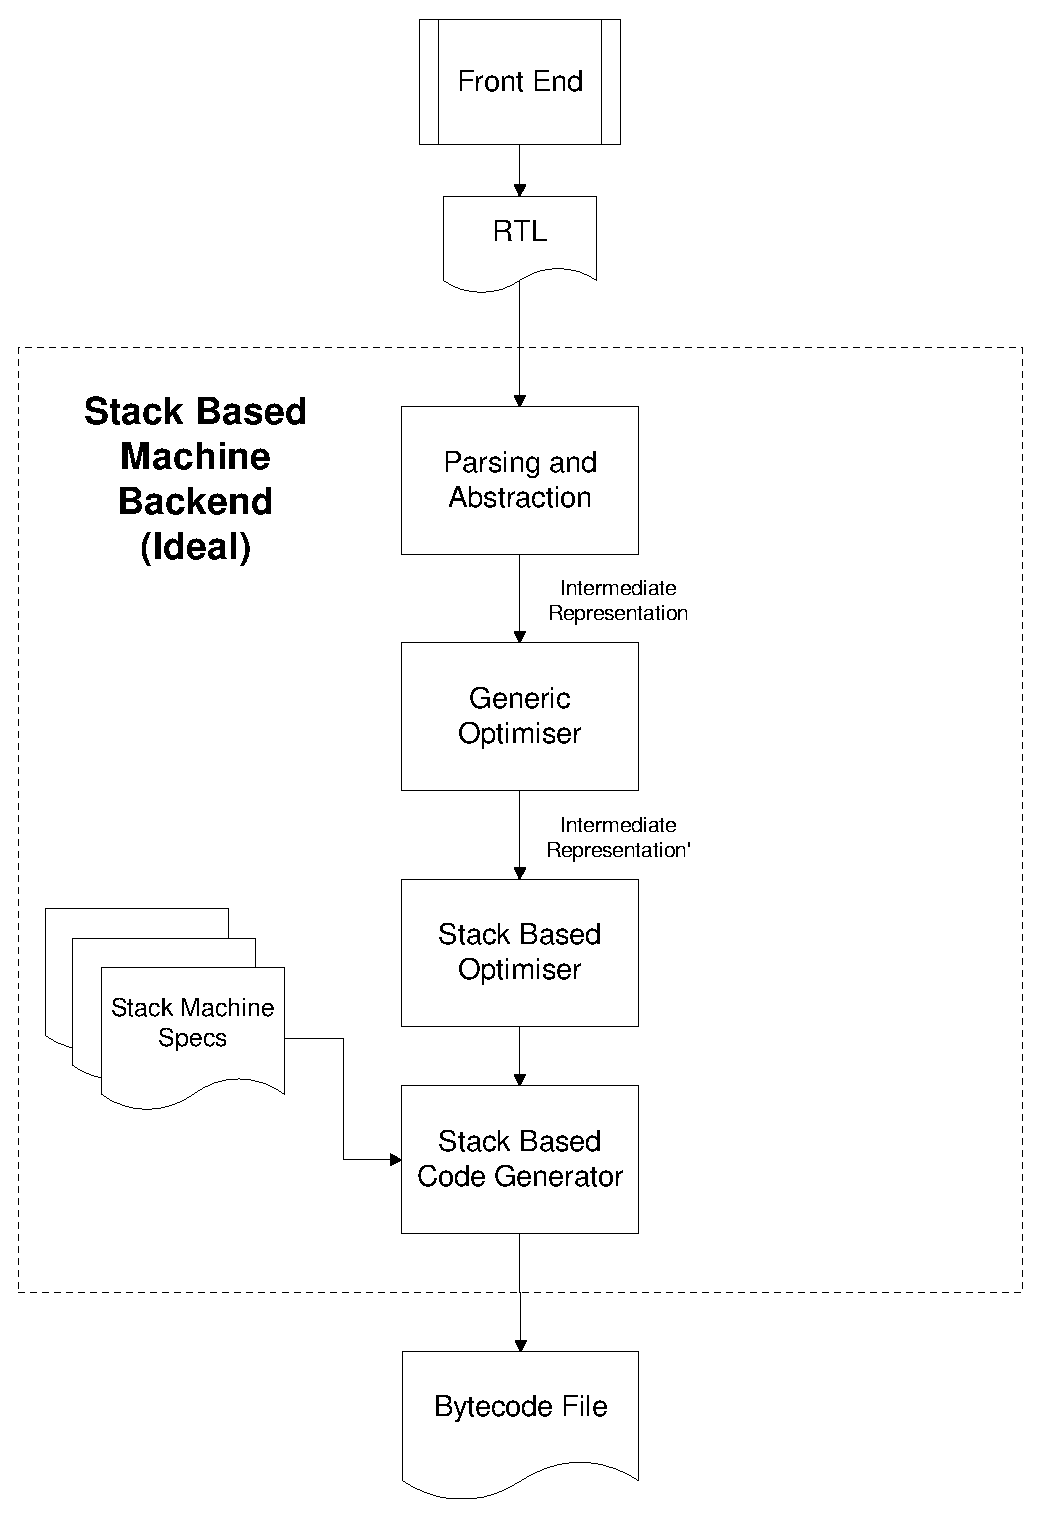
\includegraphics{figures/sbmbflow.eps}}
\centerfigend{fig-sbmbflow}{Flow Chart of the Stack Based Machine Backend}

\begin{enumerate}
\item Parsing and abstraction:  reduction of register transfer list
representation to basic assignment, call and branch statements.
\item Generic optimiser:  machine independant optimisation of those
statements.
\item Stack based optimiser:  stack based machine specific optimisations.
\item Stack based code generator:  generation of translated bytecodes
from the output of previous steps.  In the idealised model, the stack
based code generator can take a number of specification files that define
the target stack based machine.
\end{enumerate}

Each of these stages has an interface that interconnects them.  The
interface generated from parsing and abstraction of the RTL is used in the
optimiser.  This interface is known as the ``intermediate representation''
and consists of a control flow graph with each basic block containing an
array of statements.  The optimisers generate the same interface as they
receive, and as such, can be removed from the process when optimisations
are not required (such as in testing).  The code generator extends the
interface output from the optimiser with bytecode information placed in
each of the statements contained within a basic block. This data is then
linearised into an output file for the required machine.

The process depicted in figure ~\ref{fig-sbmbflow} is an idealisation of
the current experimental model of the stack based machine backend.  The
current process is better depicted in figure ~\ref{fig-sbmbflowcur} with
the difference being the final stage of processing.  Currently, the stack
based machine backend is targeted at the Java Virtual Machine and will be
hand extended to other stack based machines by rewritting this final
stage.  Once this is done, it will be easier to generalise about stack
based machines and approach the prefered model of absolute
retargetability.

\centerfigbegin
\resizebox{8cm}{!}
{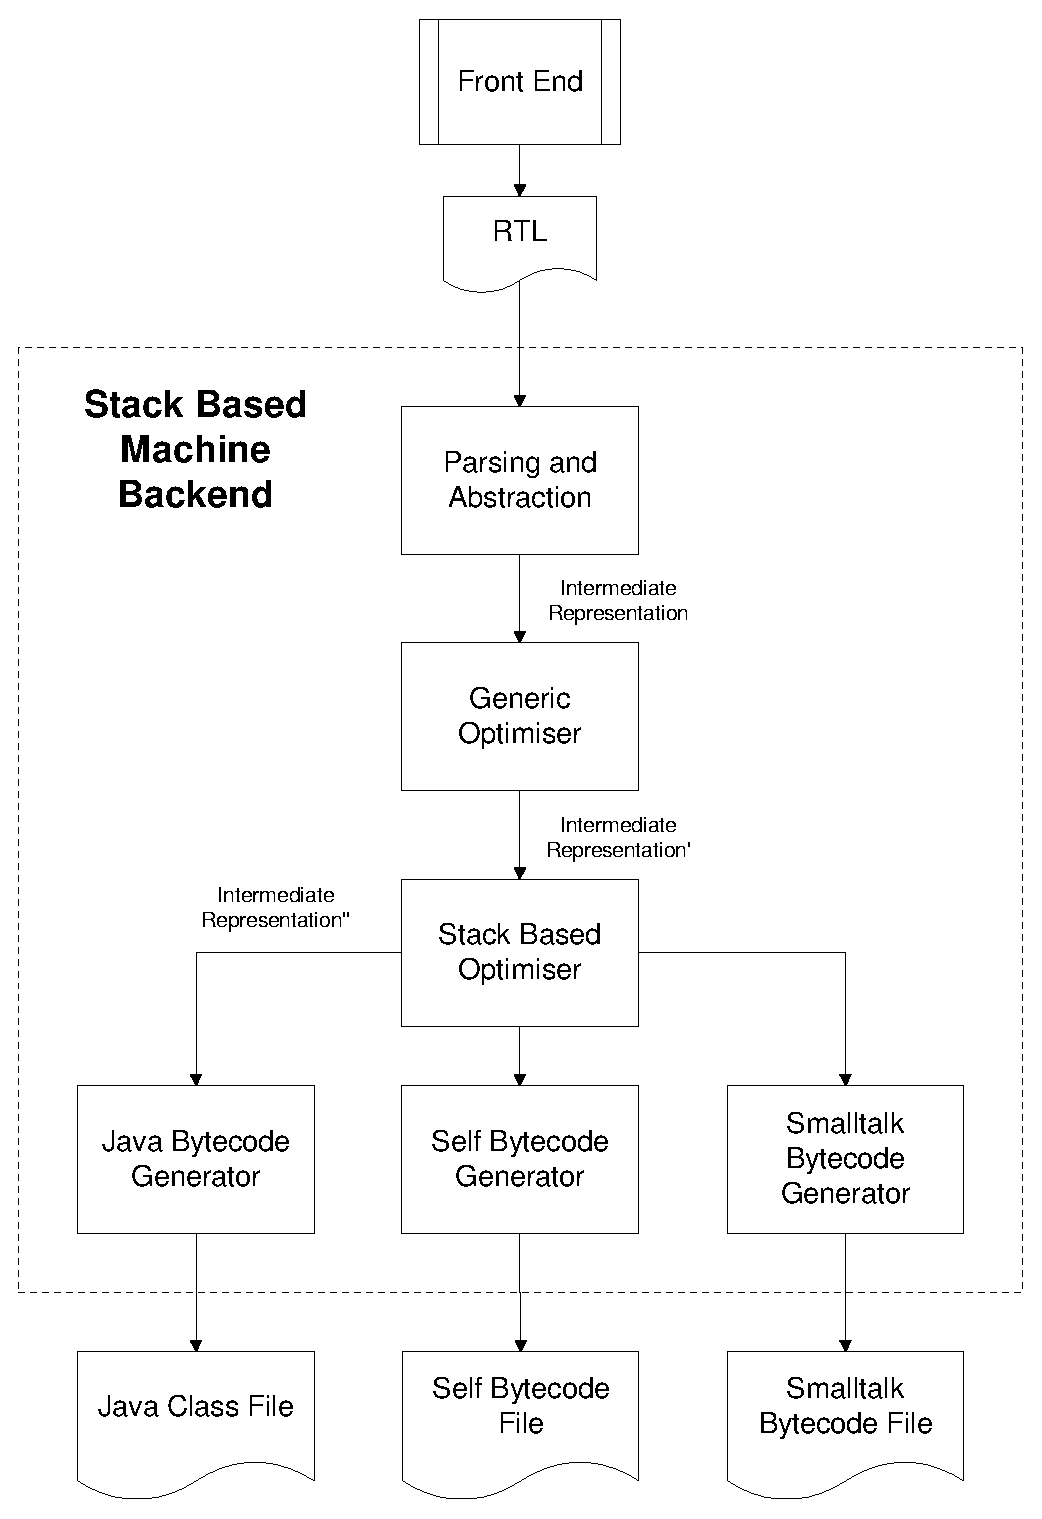
\includegraphics{figures/sbmbflowcur.eps}}
\centerfigend{fig-sbmbflowcur}{Experimental flow chart of the Stack Based Machine Backend}

\subsubsection{Intermediate Representation}

The intermediate representation consists of a control flow graph, that is,
a set of interconnected ``basic blocks''.  A basic block is defined as
having only one entry point and one exit point.  As control flows through
a program it follows a path that can be plotted.  If one was to plot all
the possible paths through a program, one would be constructing a control
flow graph.  In this way, a frontend programmer can use any form of
control structures in their language without fear of having to implement
them in the backend.  For example, an \texttt{if-then-else} structure
consists of four basic blocks.  The first basic block contains the
expression being tested.  If the expression is true, control flows to the
second basic block.  If the expression is false, control flows to the
third basic block.  Both the second and the third basic blocks fall
through to the fourth basic block.

\centerfigbegin
\resizebox{3cm}{!}
{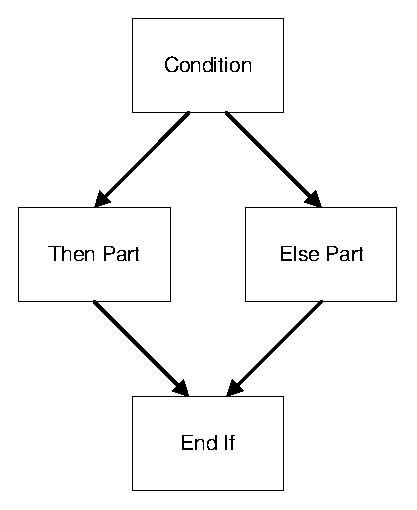
\includegraphics{figures/ifthenelse.eps}}
\centerfigend{fig-ifthenelse}{Control Flow Graph of an If-Then-Else
construct}

The first basic block is said to have two out-edges. The fourth basic
block has two in-edges.  A pretested loop is constructed just as easily.

Each basic block in the control flow graph contains an array of
statements.  These statements are mainly assignment statements but some
are also call statements.  Basic blocks which have two out edges (called
``two-ways'') have an extra statement attached, the ``conditional
statement''.  Statements are made up of expressions.  An expression can be
many things including arithmetic operations, logical operations, call and
assignment operations.  Each expression may have a number of parameters.
Expressions with two parameters are the binary expressions (add, multiply,
divide, etc).  Expressions with one parameter are the unary expressions
(negate, not, etc).  Unary expressions store their one parameter in the
``left'' node whereas binary expressions use both the ``left'' and
``right'' nodes.

These parameters are used to construct a tree structure for each
statement.  An optimiser will walk this tree structure and perform
optimisations that modify the structure.  A code generator will walk the
tree structure and generate code to be placed in various nodes of the
tree.  Both these uses of the tree structure require additional
information to be added to various nodes.  Specifying this data in the
intermediate representation classes would be non-generic and may result in
bloated trees filled with data that never gets used.  This method would
also mean that the intermediate representation would have to be changed
with every new use of the structure.  One would have to be very careful to
not ``break'' the data structure by removing anything that a user of a
previous version of the data structure may have assumed would never
change.  A solution to this problem is to allow the extension of
``objects'', that is, the instantiation of classes, not just classes
themselves.  To do this, each Java class in the implementation of the
intermediate representation is defined as an extension of the
``Extendable'' class.  A method can now be written to extend any of these
classes in such things as an optimiser or a code generator.

\subsubsection*{Data structure of the intermediate representation}

The Intermediate Representation contains a number of classes that
form a hierarchical structure of usage:
\begin{description}
\item [Program] is used to represent a complete program.  It contains an
array of procedures.
\item [Procedure] is used to represent a single procedure.  It contains
the name of the procedure and a control flow graph.
\item [BasicBlock] is used to construct a control flow graph.  It contains
a type, an array of in-edges, an array of out-edges, and an array of
statements.  Basic blocks of the \texttt{twoway} type contain a
\texttt{condition statement} which is used to determine which of the two
out-edges are followed during program execution.
\item [Expression] is used to construct statements.  Expressions contain a
type, a single integer parameter, and left and right expressions depending
on the expression type.  \texttt{Call} expressions contain an array of
expressions that are the parameters to the call.
\end{description}

\subsection{Examples}

The following examples show the current state of the UQBT frontend and the
stack based machine backend.  The following C program tests
assignments and simple conditional branches.  It is written on the SPARC 
archetecture:
\begin{verbatim}
void main() {
int i,j,k;

  j = i+k;
  k=6;
  i=j+5;

  printf("%i\n",i);
  if (j<k) 
    printf("%i\n",j);
  printf("%i\n",k);

}
\end{verbatim}
UQBT generates an output file which is parsed by the stack based machine
backend into the following statements in the intermediate representation.
\begin{verbatim}
proc main

bb type call
r[8] := r[48] 
r[9] := r[50] 
r[8] := r[8] + r[9] 
r[49] := r[8] 
r[8] := 0 | 6 
r[50] := r[8] 
r[8] := r[49] 
r[9] := r[8] + 5 
r[48] := r[9] 
r[9] := 69 << 10 
r[8] := r[9] | 552 
r[9] := r[48] 
Call printf(r[8],r[9])  

bb type twoway
r[8] := r[49] 
r[9] := r[50] 
r[0] := r[8] - r[9] 
bb cond: r[0] >= 0 

bb type call
r[9] := 69 << 10 
r[8] := r[9] | 552 
r[9] := r[50] 
Call printf(r[8],r[9])  

bb type call
r[9] := 69 << 10 
r[8] := r[9] | 552 
r[9] := r[49] 
Call printf(r[8],r[9])  

bb type ret
\end{verbatim}
These statements are passed to the code generator for Java, which adds
bytecode information to each of the nodes in the Intermediate 
Representation. Note that optimisation has been disabled for this example.  
The Intermediate Representation is then flattened to produce an output
file.  Comments have been added for clarity:
\begin{verbatim}
L0:
        iload 48        ; r[8]  := r[48]
        istore 8
        iload 50        ; r[9]  := r[50]
        istore 9
        iload 8         ; r[8]  := r[8] + r[9]
        iload 9
        iadd
        istore 8
        iload 8	        ; r[49] := r[8]
        istore 49
        ldc 0           ; r[8]  := 0 | 6
        ldc 6
        ior
        istore 8
        iload 8         ; r[50] := r[8]
        istore 50
        iload 49        ; r[8]  := r[49]
        istore 8
        iload 8         ; r[9]  := r[8] + 5
        ldc 5
        iadd
        istore 9
        iload 9         ; r[48] := r[9]
        istore 48
        ldc 69          ; r[9]  := 69 << 10
        ldc 10
        ishl
        istore 9
        iload 9         ; r[8]  := r[9] | 552
        ldc 552
        ior
        istore 8
        iload 48        ; r[9]  := r[48]
        istore 9
        iload 8         ; Call  printf(r[8],r[9])
        iload 9
        invokestatic printf
        goto L1

L1:
        iload 49        ; r[8]  := r[49]
        istore 8
        iload 50        ; r[9]  := r[50]
        istore 9
        iload 8         ; r[0]  := r[8] - r[9]
        iload 9
        isub
        istore 0
        iload 0         ; bb cond: r[0] >= 0
        ldc 0
        if_icmplt L2
        goto L3

L2:
        ldc 69          ; r[9]  := 69 << 10
        ldc 10
        ishl
        istore 9
        iload 9         ; r[8]  := r[9] | 552
        ldc 552
        ior
        istore 8
        iload 50        ; r[9]  := r[50]
        istore 9
        iload 8         ; Call  printf(r[8],r[9])
        iload 9
        invokestatic printf
        goto L4

L3:
        ldc 69          ; r[9]  := 69 << 10
        ldc 10
        ishl
        istore 9
        iload 9         ; r[8]  := r[9] | 552
        ldc 552
        ior
        istore 8
        iload 48        ; r[9]  := r[49]
        istore 9
        iload 8         ; Call  printf(r[8],r[9])
        iload 9
        invokestatic printf
        goto L2

L4:
        ret

\end{verbatim}
This bytecode is unoptimised which is to be expected as the Intermediate
Representation is unoptimised.  The generic optimiser reduces the number
of statements in the intermediate representation.  The stack based 
machine optimiser uses specific stack based machine optimisations to
reduce the number of bytecodes, local variables and stack depth.  Finally,
the code generator for the Java Virtual Machine selects the best bytecodes
to be used in the final output.

\subsection{The Runtime Environment}

Binary translation is not just a compiler backend (though it can be).  
Generally, there is a lot of code that can be shared between translated
programs.  This code has the task of emulating the environment that the
code was originally written for.  Such things as calling conventions and
dynamic linking must be known to the backend to generate code that can
link to its new environment.  We can see the need for a run time
environment through a case study.  The following C program:
\begin{verbatim} 
void main() {
  printf("hello world\n");
}
\end{verbatim}
compiles to the following assembly code (some code is removed for the
purpose of readability):

\begin{verbatim} 
.LLC0:
        .asciz  "hello world\n"

        sethi %hi(.LLC0),%o1
        or %o1,%lo(.LLC0),%o0
        call printf,0
        nop
        ret
\end{verbatim}

which can be translated and optimised to:
\begin{verbatim} 
        r[0] := .LLC0;
        call printf
        return 
\end{verbatim} 

Finally we can add to this
code the knowledge of calling convention.  On a SPARC, parameters are
passed in the first six general purpose integer registers.  The function
\texttt{printf} expects to see a pointer to an asciiz string as its first
parameter.  This is a problem in Java, for example, because \texttt{.LLC0}
refers to an offset in the source binary's read-only data section.  The
translated program will need access to this data if it is to pass the
string onto a function like \texttt{System.out.println}. The problem is
actually harder than that.  \texttt{System.out.println} expects a
\texttt{String} object type which is quite different to an asciiz string.  
The translated program will need to construct such an object using a
method not unlike the following:
\begin{verbatim} 
static String getstring(int rodatastart,byte[] rodata,int i) {
    String a = "";
      while (rodata[i-rodatastart]!=0) {
        a += (char)rodata[i-rodatastart];
        i++;
      }
      return a;
  }
\end{verbatim} 
The first parameter is the source machine address of the start of the
read-only data section.  The second parameter is a reference to the actual
bytes contained within the read-only data section.  The final parameter is
the source machine address of the asciiz string which we assume to be
located somewhere within the read-only data section.  We refer to this
calling structure as ``passing core'' and it must be used in all runtime
support libraries.

Finally the \texttt{printf} function must be written in Java to link with
the translated binary.  The function could be as simple as a wrapper to
the equivalent Java function or, in the case of printf, something more
complicated.  This must be done for every library function to be called.  
The size of a run-time environment is extensive in the case of graphical
user interface (GUI) environments.  This can be seen in the WINE
project~\cite{Wine96} which aims to emulate the Microsoft Windows
environment on 80x86 X-windows systems.  We can reuse most of the work in
that project.  This promotes the feasibility of binary translation of
Windows executables to the JVM with an interface to the awt classes.  The
biggest obstacle of the WINE project is the Application Binary Interface
(ABI) of Microsoft Windows.  Each binary refers to more than its own data
segments and system API calls.  In many operating systems, applications
have access to data structures stored in shared libraries and, as in the
case of Microsoft Windows, in the operating system itself.  These
references must be recognised by the backend and replaced with a reference
to the runtime support class.  These problems are not limited purely to
Microsoft Windows (although they appear most abundantly there), they also
pop up in SPARC binaries.  One such example is the use of \texttt{errno}
from the standard I/O C libraries.  \texttt{Errno} is a global integer
that resides in a shared library.  When it is written to, the page that is
shared is copied into the new process space.  One would wish a backend to
recognise global variables that reside in support libraries and redirect
them to the runtime support class.


\subsection{Summary}

The development of backends borrows heavily from the field of optimising
compilers.  The targeting of a backend to a stack based machine introduces
new problems in optimisation.  The JVM and its strict typing introduces
problems that have rarely been seen by compiler writers before.  A runtime
support library is necessary to minimize the size of the translated
applications and is specific to each source machine and platform.  The
development of a binary translator to Java bytecodes promises a new
mentality in application distribution.  The ``translate once, run
anywhere'' concept is already within our reach, what still awaits is a
resultant application that runs with a similar performance on the JVM as
on the source machine.  This work outlines the steps involved in such a
backend and takes the first tentative steps towards that end.



\section{gcc-jvm - A JVM Backend for the gcc Compiler} 
\label{sec-gccjvm}

{\small
\begin{flushright}
Design: Trent, Implementation: Trent, Documentation: Trent [Aug 99]
\end{flushright}
}

This section describes Trent's experiences with porting
EGCS (gcc version 1.1.2) to a stack-based machine, 
the JVM in particular.  It is written in first person.  

When I first began investigating the possibility of porting the
Experimental GNU Compilation Set (EGCS) to the Java Virtual Machine (JVM)
I thought it would be possible to semantically describe the JVM to EGCS
and have it adequately generate stack based machine byte codes.  I hoped
that I would be able to specify to the back end that the only way to load
a constant or a register (local variable) was via the stack and EGCS would
break its internal representation effectively.  This appears to be a
little too optimistic.  My attempts at constructing a machine description
where EGCS is forced to do all moves via the stack failed, not because I
was supplying too little information to the back end, but because I was
supplying too much.  This lead to an alternate strategy:  I decided to
take all the instructions that one would find on a register based machine
and implement them using a number of byte codes.  The resultant byte code
was a poor but correct representation of the original program.  Soon I had
simple programs (hello world) working and could actually perform some
benchmarks.  The results were astounding: small register transfer bound
programs ran at comparable speeds to native code.  This is best explained
with an example.

\begin{verbatim}
int fibo(int i) {
  if (i<2) return 1;
  else return fibo(i-1)+fibo(i-2);
}

void main(int argc,char **argv) {
  printf("fibo %i is %i\n",40,fibo(40)); 
}
\end{verbatim}

Fibonacci is a register transfer bound program that takes 22 seconds on a
SPARC Ultra 9 to run natively.  If we compile it to JVM byte code we get
the following (for the fibo function).

\begin{verbatim}
.method public _fibo(I)I
        .limit stack 9
        .limit locals 17
        
        iconst_0
        istore 14
        
        iload 1
        bipush 1      
        if_icmple L2
        
        iload 1  
        bipush -1
        iadd
        istore 10
        
        aload_0
        iload 10
        invokevirtual Fibo/_fibo(I)I
        istore 10   
        
        iload 10 
        istore 13
        iload 1  
        bipush -2
        iadd   
        istore 10
        
        aload_0     
        iload 10
        invokevirtual Fibo/_fibo(I)I
        istore 10
        
        iload 13 
        iload 10 
        iadd   
        istore 10
        
        goto L8     
L2:
        bipush 1
        istore 10

L8:
        iload 10 
        ireturn
.end method
\end{verbatim}

On the same machine running version 1.1 of the JVM, this bytecode takes
90 seconds to run.  The overhead is caused primarily by the two method
calls.  The following Java source code compiles to a program with the same
functionality.

\begin{verbatim}
class Fib {

  int fibo(int i) {
    if (i<2) return 1;
    else return fibo(i-1)+fibo(i-2);
  }

  void main(int argc,int argv) {                 
    System.out.println("fibo " + 40 + " is " + fibo(40));         
  }

  public static void main(String[] args) {
    Fib f = new Fib();
    f.main(0,0);
  }
}
\end{verbatim}

The resultant class file takes 56 seconds to run.  Significantly less than
the EGCS generated byte code.  The following is the byte code that is
generated by javac (for the fibo method above).

\begin{verbatim}
Method int fibo(int)
   0 iload_1
   1 iconst_2
   2 if_icmpge 7
   5 iconst_1
   6 ireturn
   7 aload_0
   8 iload_1
   9 iconst_1
  10 isub
  11 invokevirtual #13 <Method int fibo(int)>
  14 aload_0
  15 iload_1
  16 iconst_2
  17 isub
  18 invokevirtual #13 <Method int fibo(int)>
  21 iadd
  22 ireturn   
\end{verbatim}

Smaller size and less local variable usage improves the speed of the byte
code.  A possible solution to this problem is to use a post processing
optimisation stage such as BLOAT.  When applied to the poor byte code
generated by EGCS, it produces the following.

\begin{verbatim}
Method int _fibo(int)
   0 iload_1
   1 iconst_1
   2 if_icmple 31
   5 iload_1
   6 iconst_m1
   7 iadd
   8 istore_2
   9 aload_0
  10 iload_2
  11 invokevirtual #20 <Method int _fibo(int)>
  14 istore_2
  15 iinc 1 -2
  18 aload_0
  19 iload_1
  20 invokevirtual #20 <Method int _fibo(int)>
  23 istore_0
  24 iload_2
  25 iload_0
  26 iadd
  27 istore_0
  28 goto 33
  31 iconst_1
  32 istore_0
  33 iload_0
  34 ireturn
\end{verbatim}

This is still a lot more bytecodes than the javac generated output but
runs in 55 seconds.  This leads to an apparent paradox:  How can more 
bytecodes run faster than less byte codes?  The answer lies in the behaviour
of the Just In Time compiler.  For version 1.1 of the JVM one can export
an environment variable JIT\_ARGS to 'dump' to print excessive amounts of
debugging information.  Using the bash shell one would do the following
command:
\begin{verbatim}
		export JIT_ARGS=dump
\end{verbatim}

Now any execution of the JVM will result in JIT debugging information
being dumped to standard error.  For version 1.2 of the JVM one would do
the following command:
\begin{verbatim}
		export _JIT_ARGS=dump
\end{verbatim}

The following is output by the JIT for the javac generated bytecode:
\begin{verbatim}
     0 iload_1        1b     
     1 iconst_2       05           
     2 if_icmpge      a2 00 05
        subcc   %i1, 2, %g0
        bge     5
        nop     
     5 iconst_1       04     
     6 ireturn        ac
        or      %g0, 1, %i0
        ba      8
        nop        
     7 aload_0        2a           
     8 iload_1        1b     
     9 iconst_1       04
    10 isub           64   
        sub     %i1, 1, %l0           
    11 invokevirtual  b6 000d
        or      %l0, %g0, %o1
        or      %g0, %i0, %o0
        ld      [%o0 + 4], %g1
        ld      [%g1 + 52], %g1
        ld      [%g1 + 68], %g1
        jmpl    [%g1 + %g0], %o7
        nop
        unimp   0x000a5a78 
        or      %g0, %o0, %l0    
    14 aload_0        2a        
    15 iload_1        1b        
    16 iconst_2       05    
    17 isub           64
        sub     %i1, 2, %l1        
    18 invokevirtual  b6 00 0d
        or      %l1, %g0, %o1
        or      %g0, %i0, %o0
        ld      [%o0 + 4], %g1
        ld      [%g1 + 52], %g1
        ld      [%g1 + 68], %g1
        jmpl    [%g1 + %g0], %o7
        nop
        unimp   0x000a5a78 
        or      %g0, %o0, %l1    
    21 iadd           60
        add     %l0, %l1, %l0        
    22 ireturn        ac
        or      %g0, %l0, %i0
\end{verbatim}
  
The major overhead of the above code being the two method calls.  
Ignoring the method calls, ten native machine instructions are generated.  
The following is output for the BLOAT optimised EGCS output:
\begin{verbatim}
     0 iload_1        1b     
     1 iconst_1       04     
     2 if_icmple      a4 00 1d
        subcc   %i1, 1, %g0
        ble     5
        nop     
     5 iload_1        1b    
     6 iconst_m1      02
     7 iadd           60
        add     %i1, -1, %i2          
     8 istore_2       3d           
     9 aload_0        2a     
    10 iload_2        1c     
    11 invokevirtual  b6 0014
        or      %i2, %g0, %o1
        or      %g0, %i0, %o0 
        ld      [%o0 + 4], %g1
        ld      [%g1 + 200], %g1
        ld      [%g1 + 68], %g1
        jmpl    [%g1 + %g0], %o7
        nop
        unimp   0x000a5b60
        or      %g0, %o0, %l0
    14 istore_2       3d
        or      %g0, %l0, %i2         
    15 iinc           84 01fe   
        add     %i1, -2, %i1           
    18 aload_0        2a        
    19 iload_1        1b    
    20 invokevirtual  b6 0014
        or      %i1, %g0, %o1 
        or      %g0, %i0, %o0
        ld      [%o0 + 4], %g1  
        ld      [%g1 + 200], %g1
        ld      [%g1 + 68], %g1
        jmpl    [%g1 + %g0], %o7
        nop
        unimp   0x000a5b60
        or      %g0, %o0, %l0    
    23 istore_0       3b
        or      %g0, %l0, %i0        
    24 iload_2        1c        
    25 iload_0        1a           
    26 iadd           60  
        add     %i2, %i0, %i0    
    27 istore_0       3b        
    28 goto           a7 0005
        ba      1e
        nop    
    31 iconst_1       04
    32 istore_0       3b
        or      %g0, 1, %i0    
    33 iload_0        1a    
    34 ireturn        ac
\end{verbatim}

Again ignoring the two method calls, eleven native machine instructions
are generated.  One can now see that byte code size is not an entirely
fair measure of resultant JIT generated code size.

The introduction of local variable usage that cannot be mapped into
registers (for example, local arrays) a register based machine requires a
stack frame.  Commonly, a stack pointer and a frame pointer are maintained
to point to a section of volatile memory.  This posses a problem for the
JVM port: there is no generic memory.  Possible solutions are to maintain
a "stack" array of bytes and do all stack accesses to that array.  The
problem becomes more complex when one considers global memory.  The
solution I originally chose was to perform all memory input/output with a
method contained within a run time support class.  The method to read an
integer from any arbitrary point in memory was called memref and the
method to store an integer to any arbitrary point in memory was called
memstore.  These two methods would examine the address requested and
determine the required array reference: read only data, read/write data or
stack.  To perform a memory reference the backend need only generate the
following:
\begin{verbatim}
sipush 24324   ; address
invokevirtual Classname/memref(I)I
istore 9
\end{verbatim}

The resultant bytecode was very easy to read and could be easily debugged
(for example, one could monitor all reads and writes to memory).  
Unfortunately memory bound programs experienced dramatic performance
losses.  In the order of sixty times slower execution.  The solution was
to move all memory references inline and abandon the array segregation.  
All memory was placed in a single array, called "memory", in the run time
support class and now the back end is required to generate significantly
more code.  To load an integer from an unsigned byte array one need only
perform the following (big endian).

\begin{verbatim}
Register := memory[location] << 24 | 
    memory[location+1] << 16 | 
    memory[location+2] << 8 | 
    memory[location+3]
\end{verbatim}

However, the JVM does not have unsigned types, and thus each signed byte
must be converted to an integer representation of its unsigned value:
\begin{verbatim}
Register := (memory[location]<0?256+memory[location]:memory[location]) << 24 | 
    (memory[location+1]<0?256+memory[location+1]:memory[location]) << 16 | 
    (memory[location+2]<0?256+memory[location+2]:memory[location+2]) << 8 | 
    (memory[location+3]<0?256+memory[location+3]:memory[location+3])
\end{verbatim}

To improve the performance of each integer memory reference, the memory
array is made an array of int instead of an array of byte.  Initialised is
then put into the array already in unsigned format.  The speed increase
comes at the expense of a 4:1 increase in space requirements.  The
following code is generated by the back end to perform an integer memory
reference:
\begin{verbatim}
        aload_0
        getfield Classname/memory [I
        iload 12 ; address
        dup2  
        iaload  
        bipush 8
        ishl
        dup_x2
        pop 
        iconst_1
        iadd
        dup2
        iaload   
        bipush 16
        ishl    
        dup_x2  
        pop 
        iconst_1
        iadd
        dup2
        iaload
        bipush 8
        ishl     
        dup_x2   
        pop     
        iconst_1
        iadd
        iaload  
        ior 
        ior 
        ior
        istore 11  ; destination
\end{verbatim}

The same memory bound benchmarks now run at 20 to 30 times as slow.  
Memory management is still a significant issue that is difficult to
resolve.


\subsection*{The build process}

The output of the compiler proper is one jasmin~\cite{Meye97} 
assembler file per C language input file.  
If the input files contain no global data, the build
process is simple, concatenate the multiple jasmin files into a single
file and assemble to a class file.  However, C files containing global
data produce an addition output file global.s.  References to labels
contained in global.s will appear in the jasmin output preceded by
"symref" and proceeded by "end".  As each C input file is compiled, the
global.s outputs are concatenated together into gglobal.s.  This file is
assembled to object format and a search and replace program (sed) is used
to replace each symbol reference with an offset into the data section.  
Finally the object file is objcopied into a raw data file and passed to
the run time support class to be loaded into the memory array.  This
process is only needed in programs with multiple input files and global
data.


\section{The Java JVM Back end}
\label{sec-jvmbackend}

{\small
\begin{flushright}
Design: Cristina and Brian, Implementation: Sameer [Aug 00], Brian [Nov 00],  
	Documentation: Brian [Nov 01]
\end{flushright}
}

The Java JVM back end is a rewrite of the C-based original JVM 
back end that was written in early 1999.  We were interested in 
seeing whether the Java language could be used to write back ends 
for our translator needs.  The following notes explain part of the
operation of this back end. 
Experience with the user of this back end is described in the 
{\emph{Experience}} chapter (Chapter~\ref{ch-experience}) in 
Section~\ref{sec-to-jvm}.  

The Java JVM backend operates much like the C and other backends. 
Unlike the C (Chapter~\ref{ch-cbackend}) and the VPO (Chapter~\ref{ch-vpobackend}) 
backends, however, it is single-pass. The Jasmin code for each procedure is
emitted in one pass. A small runtime library implemented in the file
\texttt{TranslatedFile.java} provides support for the generated code. That 
file contains a method \texttt{realMain} that is called first when the 
translated program starts execution. The \texttt{realMain()} method 
initializes the memory used by the translated program and copies the program's 
command line arguments into that memory.  The \texttt{realMain()} method 
then calls the translated program's \texttt{\_main()} method, which contains 
the code for the program's main procedure. All generated methods are static 
except for \texttt{\_main()}. This is done for technical reasons 
(\texttt{\_main} is declared abstract in \texttt{TranslatedFile.java}).

It recursively processes a source procedure's HRTLs for a procedure and
emits directives for each HRTL into a Jasmin source file. Given a HRTL, it
checks first whether it is a high-level HRTL such as a CALL\_HRTL, or if it
is a RTLList, a list of low-level RTLs. If the former, directives for the
control transfer or other high-level HRTL are emitted. If the latter,
directives for each RTL in the list are emitted. A postorder traversal of
each RTL's subexpressions produces the stack-oriented JVM bytecodes for that
RTL. 

Memory is represented using a single large Java byte array "memory". The
source program's bss and data segments are read into the appropriate
elements of that array so that a data item at a particular
address x can be read from memory[x].

The most complex thing (perhaps) about the JVM backend's operation is its
allocation of JVM locals for the HRTL variables:

\begin{itemize} 
\item Local 0 always holds the Java \texttt{this} reference if the procedure 
	is \texttt{\_main()}, and the first procedure argument otherwise.
\item Locals 1-7: all or remaining formal parameters (assumes there are 
	up to 6 parameters at most).
\item Local  8 and 9: unused.
\item Local [10..(10+n)): the n local HRTL variables used in the method.
\item Locals [(10+n)..99]: the HRTL temporary registers.
\item Local 100: a temporary variable used for, e.g., byte swapping.
\end{itemize}


\subsection{Usage of the Java JVM Backend}
To use the JVM backend,
build \uqbt\ with \texttt{with-target=sparc}
and then request the JVM backend using the command line option \texttt{-j}.
This will make \uqbt use the JVM backend
rather than the default low-level \texttt{C} backend.
The \texttt{Makefile} generated in the output directory created by \uqbt\ 
includes rules to run Jasmin and build the necessary Java class files for
the translated program.


	 % JVM backend (two different versions) 

	
\chapter{The VPO Back End}
\label{ch-vpobackend}

{\small
\begin{flushright}
Design: Mike, Cristina, Norman. Implementation: Mike [98], Brian [01]. 
Documentation: Mike [98], Cristina, Brian [01]
\end{flushright}
}

In early 1998 we were using the VPO (very portable optimizer) system  
by Jack Davidson and students, University of Virginia, as our 
optimizer of choice.  We experimented with SPARC translations 
before we moved onto the C back end (see Chapter~\ref{ch-cbackend}). 
VPO's RTL interface back then was new and did not support x86 or 
other machines yet. 
The 1998 VPO back end is described in Section~\ref{sec-vpo}. 
This section is useful for historical reasons. 

In 2001 we went back to use VPO for optimization, by then, VPO's 
new RTL interface supported not only SPARC, but also x86 and ARM 
amongst other machines.  We were interested in translations to 
these three machines.  The original 1998 VPO back end was revived 
in a new form and made much more extensible and robust. 
The 2001 VPO back end is described in two parts: first, the 
experiment in translating IRTL to SPARC VPO RTLs is described in 
Section~\ref{sec-irtlvpo}, and next, the experiences with translating 
\hrtl\ to ARM VPO RTLs are described in Section~\ref{sec-vpo2001}. 


\section{The 1998 VPO Back End}
\label{sec-vpo}

This section describes \texttt{vpoback}, an experimental RTL$_{UQ}$
to RTL$_{VPO}$ translator which generates a file suitable for
piping to VPO, so that an executable file can be generated.
This backend is not meant to
be a serious prototype for a real backend, but is intended to demonstrate
the compatibility of the two RTLs. The experiment was
a success; it was possible to translate enough RTLs to generate a simple 
``hello world'' binary executable file for the SPARC platform (from 
a SPARC source binary).


\subsection{Description}

The experimental backend has been written to work with a preliminary
version of the VPO interface, as supplied by the University of Virginia 
in February 1998. This version has two distinct interfaces; one to generate 
Register Transfer Lists, and one to handle higher level concepts such as 
functions and global symbols. All functions of the first interface have 
names beginning with \texttt{Rtl\_}, while functions of the latter interface 
have names beginning with \texttt{VPOi\_}.


\subsection{Handling expressions}
\label{sec-expr}

In general, expressions in VPO are very similar to expressions in our
RTlists. For binary expressions, there are two considerations when
translating from RTL$_{UQ}$ to RTL$_{VPO}$. Firstly,
the operators have to be translated. Secondly, the \texttt{sethi}
instruction has to be considered specially. Most of our operators have
direct VPO equivalents. Notable exceptions are rotates with carry
(RTL$_{VPO}$ does not have them), and bit extractions (RTL$_{VPO}$ does
not appear to have them).

When translating the \texttt{sethi} instruction, it was found necessary
to translate
expressions of the form \verb!K << 10! (where K is a constant, and
\verb!<<! represents the left shift operator) to expressions like
\texttt{HI[X]}, where \texttt{HI} is a special Sparc specific unary
operator in VPO, and X has the value \verb!K<<10!.


\subsection{Handling registers}

Normal machine registers, such as r[8] (and even r[0] for register \%g0)
translate
directly to VPO using the \texttt{Rtl\_constLoc()} function. Some registers
are named (i.e. they are represented as a \texttt{Register} object, whose
\texttt{Index} member points to an object of type \texttt{Constant}, whose
value is a string, e.g. ``\%fp''). Others are implemented as special
registers (i.e. they are represented as a \texttt{SpecialReg} object).
SpecialReg objects have a name (it could also be \texttt{\%fp}; both
representations exist at present). These named registers
are translated into the appropriate general purpose register (\texttt{\%fp}
maps to register 30, and \texttt{\%sp} maps to register 14).

Temporary registers (e.g. \texttt{r[\_\_tmp123]}) are translated to ordinary
registers beginning with index 51 (for texttt{r[\_\_tmp001]}). VPO is to be
changed so that temporary registers will occupy their own storage spaces.


\subsection {Handling memory}

An object of class Memory contains a pointer to a Value object, which
could be of three types: \texttt{eCONSTANT}, \texttt{eREGISTER}, or
\texttt{eSPECIALREG}. These
represent the address of the memory being referenced. Where the address
is constant, the \texttt{Rtl\_constLoc()} function is used. Where the address
is given as a register, the register is processed as a location. This
location is fetched using \texttt{Rtl\_fetch()}, and the resultant expression
is used as the operand to \texttt{Rtl\_location()}.


\subsection {Handling RT assignments}

RT assignments involve a location and an expression. The location will
be either a register or memory object; each of these is translated to
a VPO location as above. The expression is also translated as previously
described (section~\ref{sec-expr}).
Where registers or memory are involved in the expression, they are translated 
as described above, and the result is converted into a value using
the \texttt{Rtl\_fetch()} function. The location and expression resulting
from the above (of types \texttt{Rtl\_ty\_loc} and \texttt{Rtl\_ty\_expr}
respectively) are
combined and emitted using the \texttt{VPOi\_rtl()} interface function.


\subsection {Handling Control Transfer instructions}

All the above translations are handled by considering a single Register
Transfer (RT) at a time. Basically, each RT of each RTL in the function
of interest is examined in a double counter for loop. However, there are a few
situations that have to be handled by examining a whole RTL; control
transfer instructions and frame instructions are examples. Complex
code examines each RTL to see if it matches the pattern of the appropriate
instruction of interest; if so, code is emitted to VPO directly instead
of translating the whole list of RTs separately. It is hoped that changes
to the representation for RTL$_{UQ}$ will simplify this comparison.

If the instuction is recognised as a control transfer instruction, more
complex code decides whether the instruction is a conditional or
unconditional branch, call, or return instuction. (This complex, difficult
to debug code may one day be automatically be generated by some sort of
tool given a piece of specification or RTL tree).

Return instuctions are simple; an assignment from register \texttt{RT}
(a special
VPO pseudo register) to register texttt{PC} is emitted.

For a call instruction, a symbol has to be generated for the destination
of the call. (This will become a call to the ``assembly interface'' one
day; at present, it is a VPOi function). At the time of writing, the
names of dynamic symbols was not available, so the function name is
fixed at ``printf''. The call is generated by emitting an assignment to
special VPO register ST (``STack''?) from the global symbol for the
destination of the call. In order to convince VPO that main was not a
leaf function, we had to use the \texttt{VPOi\_registerUse()} function,
with an argument list including all registers
from 1 to 15, indicating that all these registers had to be saved across
the call (and therefore, leaf optimisation for the procedure containing
the call is not possible).

Unconditional branches are not implemented as of this writing; they should
present no special problems beyond those required for a call.

Conditional branches in VPO have the form \texttt{PC=IC:0,L1234} where
\texttt{PC} of course represents the program counter, \texttt{IC} represents
the integer condition code register, the colon represents a relational 
operator, and \texttt{L1234} represents
a label. This is emitted as a guarded assignment, using \texttt{Rtl\_guard()}
and \texttt{Rtl\_Rtl\_assign()}. The required operator has to be determined
from an
expression contained in the RTL for the branch instruction (it depends
on the condition codes used, as well as the operators, and whether
the condition code is used directly, or negated first). This is again
difficult to write code that may be automated in the future.

As an example of this process, consider the \texttt{bg} (branch if signed
greater) Sparc instruction. There are three RTs in the RTL; the
%main RT contains the subexpression \texttt{\~(\%Z \| (\%N \^ \%V))}
main RT contains the subexpression \verb!~(%Z | (%N ^ %V))!
(where \verb!~!
represents logical negation, and \verb!^! represents the exclusive OR
operator). When this subexpression is detected, the VPO opertor required
is \texttt{Rtl\_op\_gt}.

It was found that VPO does not have suitable operators for handling
the jump if positive/negative instructions, and jump on overflow /
no overflow.


\subsection {Processing Frame instructions}

The save and restore instructions (which establish and remove stack
frames) are recognised at the RTL level, just as conditional control
transfer instructions are. At present, only the restore instruction
is correctly recognised, and this is used to call the
\texttt{VPOi\_functionEnd()} function.


\subsection {Other VPO calls}

The function \texttt{premble()} calls several VPOi functions that are
needed to
initialise VPO itself, and to set up a label for \texttt{main}. These
functions
set up the register map and special location map; both of these are
going to be changed in the next version of the VPO interface.


\subsection {Sample Generated Code}

This output is from an early version. It should be replaced by a later
version.

The input file was compiled from the folowing source by {\it gcc}:
\begin{verbatim}
#include <stdio.h>

int main()
{
    int a=5; int b=7;
    unsigned u=5; unsigned v = 7;

    if (a == b) printf("Equal\n");
    if (a != b) printf("Not Equal\n");
    if (a >  b) printf("Greater\n");
    if (a <= b) printf("Less or Equal\n");
    if (a >= b) printf("Greater or Equal\n");
    if (a <  b) printf("Less\n");
    if (u >  v) printf("Greater Unsigned\n");
    if (u <= v) printf("Less or Equal Unsigned\n");
    if (u >= v) printf("Carry Clear\n");
    if (u <  v) printf("Carry Set\n");
}
\end{verbatim}

Generated output (filtered by the \texttt{decode} program and formatted for
3 columns):
\begin{verbatim}
-   .seg    "text"      +r[51]=r[8]             +r[16]=R[r[51]]
-    .global _start     +R[r[51]]=r[11]         +r[17]=r[14]-r[9]
-_start:                +r[51]=r[30]+20         +PC=ICs0,L67452
+r[30]=r[0]|0           +r[16]=R[r[51]]         +r[8]=66{10
+r[51]=r[14]+64         +r[51]=r[30]+24         +r[30]=r[0]|232
+r[16]=R[r[51]]         +r[16]=R[r[51]]         +r[51]=r[30]+28
+r[17]=r[14]+68         +r[17]=r[14]-r[9]       +r[16]=R[r[51]]
+r[17]=r[14]-32         +PC=IC!0,L67236         +r[51]=r[30]+32
+r[30]=r[0]|r[1]        +r[8]=66{10             +r[16]=R[r[51]]
+PC=IC:0,L66984         +r[30]=r[0]|144         +r[17]=r[14]-r[9]
+r[30]=r[0]|r[1]        +r[51]=r[30]+20         +PC=ICh0,L67488
+r[8]=66{10             +r[16]=R[r[51]]         +r[8]=66{10
+r[30]=r[0]|116         +r[51]=r[30]+24         +r[30]=r[0]|256
+r[30]=r[0]|r[16]       +r[16]=R[r[51]]         +r[51]=r[30]+28
+r[30]=r[0]|r[17]       +r[17]=r[14]-r[9]       +r[16]=R[r[51]]
+r[10]=r[16]{2          +PC=IC:0,L67272         +r[51]=r[30]+32
+r[17]=r[14]+4          +r[8]=66{10             +r[16]=R[r[51]]
+r[17]=r[14]+r[10]      +r[30]=r[0]|152         +r[17]=r[14]-r[9]
+r[8]=130{10            +r[51]=r[30]+20         +PC=ICl0,L67524
+r[30]=r[0]|572         +r[16]=R[r[51]]         +r[8]=66{10
+r[51]=r[10]            +r[51]=r[30]+24         +r[30]=r[0]|280
+R[r[51]]=r[11]         +r[16]=R[r[51]]         +r[51]=r[30]+28
*                       +r[17]=r[14]-r[9]       +r[16]=R[r[51]]
+r[8]=64{10             +PC=IC'0,L67308         +r[51]=r[30]+32
+r[8]=64{10             +r[8]=66{10             +r[16]=R[r[51]]
+r[30]=r[0]|824         +r[30]=r[0]|168         +r[17]=r[14]-r[9]
+r[17]=r[14]+r[15]      +r[51]=r[30]+20         +PC=ICg0,L67560
+r[8]=0{10              +r[16]=R[r[51]]         +r[8]=66{10
+r[30]=r[0]|4           +r[51]=r[30]+24         +r[30]=r[0]|296
+r[51]=r[23]+r[8]       +r[16]=R[r[51]]         +r[30]=r[0]|0
+r[16]=R[r[51]]         +r[17]=r[14]-r[9]       *
+r[51]=r[8]+4           +PC=IC>0,L67344         +r[8]=64{10
+r[16]=R[r[51]]         +r[8]=66{10             +r[8]=64{10
+r[17]=r[14]-0          +r[30]=r[0]|184         +r[30]=r[0]|308
+PC=IC:0,L67144         +r[51]=r[30]+20         +r[17]=r[14]+r[15]
+r[17]=r[14]+4          +r[16]=R[r[51]]         +r[8]=0{10
+r[51]=r[16]            +r[51]=r[30]+24         +r[30]=r[0]|8
+r[16]=R[r[51]]         +r[16]=R[r[51]]         +r[51]=r[23]+r[8]
+r[17]=r[14]+4          +r[17]=r[14]-r[9]       +r[16]=R[r[51]]
+r[51]=r[16]            +PC=IC<0,L67380         +r[51]=r[8]+4
+r[16]=R[r[51]]         +r[8]=66{10             +r[16]=R[r[51]]
+r[17]=r[14]-0          +r[30]=r[0]|200         +r[17]=r[14]--1
+PC=IC!0,L67116         +r[51]=r[30]+20         +PC=IC:0,L67660
+r[30]=r[0]|5           +r[16]=R[r[51]]         +r[17]=r[14]+-4
+r[51]=r[8]             +r[51]=r[30]+24         +r[51]=r[16]
+R[r[51]]=r[11]         +r[16]=R[r[51]]         +r[16]=R[r[51]]
+r[30]=r[0]|7           +r[17]=r[14]-r[9]       +r[17]=r[14]+-4
+r[51]=r[8]             +PC=IC`0,L67416         +r[51]=r[16]
+R[r[51]]=r[11]         +r[8]=66{10             +r[16]=R[r[51]]
+r[30]=r[0]|5           +r[30]=r[0]|224         +r[17]=r[14]--1
+r[51]=r[8]             +r[51]=r[30]+28         +PC=IC!0,L67632
+R[r[51]]=r[11]         +r[16]=R[r[51]]         *
+r[30]=r[0]|7           +r[51]=r[30]+32
\end{verbatim}

This is a brief summary of the interace functions used by \texttt{vpoback}.

\subsection {RTL Interface}
\begin{tabular}{l l}
Rtl\_unary      & Generates a unary expression \\
Rtl\_binary     & Generates a binary expression \\
Rtl\_fetch      & Converts a location to an expression \\
Rtl\_op\_special & Generates a special RTL operator \\
Rtl\_int        & Generates an integer as an expression \\
Rtl\_location   & Generates a location \\
Rtl\_constLoc   & Generates a location from a space and an index \\
Rtl\_assign     & Generates an RT assignment from a location and expression \\
Rtl\_guard      & Generates a sort of guard (for conditional branches) \\
Rtl\_label      & Generates a label (e.g. \texttt{L1234}) \\
Rtl\_globalSymbol & Generates a global symbol (e.g. \texttt{printf}) \\
\end{tabular}

\subsection {VPOi Interface}
\begin{tabular}{l l}
VPOi\_rtl		& Sends an RTL to output \\
VPOi\_registerMap 	& Sends a register map line to output \\
VPOi\_specialLocationMap & Tells VPOi about the special locations \\
VOIi\_assembly    	& Generate assembler directives \\
VPOi\_functionName 	& Tells VPOi about a function \\
VPOi\_functionEnd 	& Tells VPO and VPOi that a function has ended \\
VPOi\_variableDeclaration & Sends a variable definition to output \\
VPOi\_registerUse  	& Sends register use information to output \\
\end{tabular}


\section{Initial 2001 Experiments with VPO -- Translating IRTL to VPO RTLs}
\label{sec-irtlvpo}

{\small
\begin{flushright}
Design: Brian;
Documentation: Brian;
Implementation: Brian [June 01]
based on Mike's 1998 SPARC VPO backend.
\end{flushright} 
}

The IRTL Sparc-to-VPO backend uses the
University of Virginia's Very Portable Optimizer (VPO)
to generate optimized SPARC code
from an IRTL ({\em not} HRTL) representation of a source SPARC
program.
The quality of the optimized code is about the same as produced by gcc
with optimization level \texttt{-O4}.
IRTLs ({\em intermediate RTLs}) are a representation of programs
that is close to the machine level.
IRTLs differ from RTLs primarily in having
delayed branch instructions removed.
They differ from HRTLs in being source machine-specific
and not having the additional information about,
for example, procedure parameters and return values,
that results from expensive HRTL analysis.

This backend is experimental and incomplete.
It cannot translate some programs where the more sophisticated (and
expensive) HRTL analysis is required.
For example, the test program \texttt{paramchain}
requires information about return values
that is only provided by HRTL analysis.
The IRTL backend also does not currently support switch statements
(although this would be relatively easy to add).
The IRTL backend passes about 75\% of the \uqbt regression tests.  

VPO provides instruction selection, instruction scheduling, and classical
global optimization.
VPO has been retargeted to a wide variety of architectures
including the SPARC, ARM, Pentium, and MIPS.
It operates on programs that are represented as register-transfer lists (RTLs).
These RTLs resemble those used by UQBT but are lower-level,
the expressions allowed are simpler.
While the VPO RTL language itself is machine-independent
(VPO has been used with several C front ends),
VPO RTLs encode target machine-specific information.
A VPO RTL is required to represent one target machine instruction.
This is called the {\em VPO invariant}.

Mike van Emmerik had done some initial experiments with VPO in 1998
that showed that VPO could be effective for optimizing translated programs.
One objective of the current work was to experiment further with VPO.
Another was to explore the use of a backend
that translates UQBT IRTLs into VPO RTLs.
IRTLs ({\em intermediate RTLs}) are a representation of programs
that is close to the machine level.
IRTLs differ from RTLs primarily in having
delayed branch instructions removed.
They differ from HRTLs in being source machine-specific
and not having the additional information about,
for example, procedure parameters and return values,
that results from expensive HRTL analysis.
The expectation was that it would be
straightforward to translate the low-level IRTLs into VPO RTLs
for the same machine.
A secondary goal was to explore how effective IRTLs are
as a basis for translations
when the target machine is the same as the source machine.
IRTLs are inexpensive to create compared to HRTLs,
but it was unclear whether additional information would be required.


\subsection{Design of the IRTL to VPO backend}

The SPARC IRTL to VPO backend (``VPO backend'')
is structured much like the other UQBT back ends.
The VPO backend is called for each procedure
to emit code for its IRTLs.
It does not directly emit code 
but instead emits VPO RTLs and other directives
that are written to a file \texttt{{\em procname}.cex}.
The VPO backend makes use of a small library,
the VPO input library {\em VPOi},
to produce the .cex file.
The Makefile generated for a translated program 
later invokes the VPO optimizer on each .cex file
to generate an optimized assembler source file.
That .s file is then assembled to produce a .o file
for each procedure of the source program. 

The VPO backend has two passes.
A first pass scans each basic block and IRTL
in order to discover what variables, labels, and procedures
need to be declared to VPO.
A second pass then processes each IRTL to emit the
necessary VPO RTLs and directives.
A recursive walk is made of each IRTL expression.
IRTL expressions (and so IRTLs) are higher-level than VPO RTLs
since they may require several target machine instructions to implement.
For example, the single IRTL

\begin{verbatim}
000109ec *32* r[8] := m[r[16] + 948]
\end{verbatim}

requires three SPARC instructions and so at least three VPO RTLs.


\subsubsection{IRTL in more detail}
While IRTL is close to the machine level
and to UQBT RTLs,
some machine-specific details have been abstracted away.
As mentioned above,
IRTL does not contain information about delayed branches.
This is useful for a VPO backend 
since VPO does not support the specification of delayed branches
in its input RTLs.
IRTL also does not contain information about 
whether a procedure in the source program was a leaf procedure
or whether it had a register window (used \texttt{save} and \texttt{restore}).
Detailed information about a procedure's entry prologue and epilogue
are abstracted away.
For example, when a procedure returns an integer result,
the IRTLs describing the semantics of a return
specify the semantics from the viewpoint of the caller
(the caller's \texttt{\%O0} register is set)
and do not indicate how the original procedure returned that value:
whether it stored into \texttt{\%O0} or \texttt{\%i0}.

Although IRTL does not reflect the extensive analysis done for HRTL,
some analysis is done.
For example, each basic block is identified and categorized.
Also, switch statements are recognized and analyzed,
and the resulting IRTL includes data structures describing 
each switch statement.
The IRTL for a switch also includes a synthesized variable for
the switch index in place of, say, the machine register 
containing the original index.


\subsection{Status of the VPO backend}
The VPO backend currently passes 34 (75\%) of our 45 regression tests.
This compares with 33 for the Expander backend which,
although it has access to the more precise HRTL information,
does not implement floating point.
The VPO backend does not implement switch statements yet.
This would be easy to do (perhaps needing three days),
and would enable the backend to pass an additional five tests.


\subsubsection{Performance}
Table~\ref{tab-perf} shows the performance of the VPO backend
compared to optimized gcc (gcc -O4) for a number of small programs.
The backend does not currently run larger programs such as compress
so these figures are only a rough indication of the backend's 
ability, through VPO, to generate efficient code.
The time required to run each program is given in seconds.
Source programs were compiled using gcc 2.8.1
using both -O0 and -O4.
All programs were run on an otherwise idle 451 MHz Sun 420R with 4GB of RAM
running Solaris 2.8.

\begin{figure}[htb]
\center
{\small
\begin{tabular}{|l|c|c|}
\hline
 {\em Program}            & {\em gcc -O4} & {\em VPO backend} \\
\hline
\hline
 \verb#Fibo-O0 (40)#      & \verb#9.9#    & \verb#21.5#       \\
 \verb#Fibo-O4 (40)#      & \verb#10.2#   & \verb#11.8#       \\
 \verb#Sieve3000-O0#      & \verb#10.3#   & \verb#12.4#       \\
 \verb#Sieve3000-O4#      & \verb#12.0#   & \verb#11.1#       \\
 \verb#MBanner-O0 (500K)# & \verb#47.7#   & \verb#51.0#       \\
 \verb#MBanner-O4 (500K)# & \verb#18.0#   & \verb#13.4#       \\
\hline
\end{tabular}
}
{\caption{\label{tab-perf}{Performance - gcc versus SPARC IRTL to VPO backend}}}
\end{figure}

Performance of the VPO backend's version of Fibo-O0
suffers because the source program kept its input argument
in memory rather than a register
and stored it in the caller's frame.
While the VPO backend can optimize references to local variables
(caching them in machine registers),
it was unable to optimize 
the many references to memory for the input argument.
The VPO version of Sieve3000-O0 is slightly slower
because VPO still emitted many unnecessary register to register moves.
There is a chance that this performance could be improved 
by giving VPO more precise information 
about the lifetimes of temporary locations.


\subsection{Experience}
This section describes various things that were learned 
during the development of the IRTL to VPO backend.
The next section summarizes the lessons learned during this work.

\subsubsection{Need for procedure argument and return analysis}
The most significant item learned during this work
was that analysis of procedure argument and return value information
is required for a VPO backend to correctly generate code.
This is unfortunate since that analysis is expensive.
The reason for this is ultimately that VPO requires detailed information 
about the lifetime of each location
(machine register or memory location).
A client program must specify for each procedure call
what locations contain parameters
and what locations will contain return values.
The VPO backend does not have this information,
with the result that many programs do not run,
in particular the larger, more realistic (representative) ones.

Currently, the VPO backend assumes that up to six parameters are passed
and that they are passed in the SPARC registers \texttt{\%o0} to \texttt{\%o5}.
This is clearly not enough for many programs,
and is not a correct assumption.
It also may result in VPO generating suboptimal code
since it must, e.g., reserve space for possibly unused parameters
in the calling frame.
However, this assumption was sufficient
to continue the backend's development long enough
to make significant progress and to discover other issues.

Analysis must also be done to discover information about return values.
The test program \texttt{paramchain} illustrates this need:

\begin{verbatim}
void addem(int a, int b, int c, int* res) {
    *res = a+b+c;
}

void passem(int a, int b, int c, int* res) {
    addem(a, b, c, res);
}

int main() {
    int res;
    passem(5, 10, 40, &res);
    printf("Fifty five is %d\n", res);
    return 0;
}
\end{verbatim}

When \texttt{paramchain} is compiled -O4 without inlining,
the following SPARC code is produced for 
procedures \texttt{passem} and \texttt{addem}:

\begin{verbatim}
addem()
	10934:  82 02 00 09        add     	%o0, %o1, %g1
	10938:  82 00 40 0a        add     	%g1, %o2, %g1
	1093c:  81 c3 e0 08        jmp     	%o7 + 8
	10940:  c2 22 e0 00        st      	%g1, [%o3]
	10944:  00 00 00 00        unimp   	0x0
	10948:  00 00 00 00        unimp   	0x0
	1094c:  00 00 00 00        unimp   	0x0
	10950:  00 00 00 00        unimp   	0x0
passem()
	10954:  82 10 00 0f        mov     	%o7, %g1
	10958:  7f ff ff f7        call    	addem
	1095c:  9e 10 00 01        mov     	%g1, %o7
\end{verbatim}

Note the unusual code for \texttt{passem}.
While it is a leaf procedure,
it makes a call.
The two instructions surrounding the call
save then restore the return location in \texttt{\%o7}
so that \texttt{addem} will return,
not to it,
but directly to its caller, \texttt{main}.
However, information about these instructions 
is lost in the IRTLs for these procedures:

\begin{verbatim}
IRTLs for procedure addem:
Ret BB (0x3da430):
00010934 *32* r[tmp] := r[8]
         *32* r[1] := r[8] + r[9]
00010938 *32* r[tmp] := r[1]
         *32* r[1] := r[1] + r[10]
0001093c *32* m[r[11]] := r[1]
0001093c  RET

IRTLs for procedure passem:
Call BB (0x3b82e8):
0010954  CALL addem()

Ret BB (0x3b81d8):
00000000  RET
\end{verbatim}

Since \texttt{passem} makes a call,
VPO will have it use a register window.
But this code is incorrect since then \texttt{addem}
(which VPO will make a leaf procedure)
will store its result in the memory location pointed to by \texttt{r[11]},
or \texttt{\%o3},
of \texttt{passem}, not \texttt{main} as intended.
Furthermore, the value stored will be based on the uninitialized
\texttt{\%o0} through \texttt{\%o2} of \texttt{passem},
not of the intended \texttt{main}.

Even if VPO were to make \texttt{passem} a leaf procedure
(so that \texttt{addem} reads then stores into \texttt{main's} variables),
the code still doesn't work since then 
\texttt{passem} will return to the wrong procedure:
not to \texttt{main} but to \texttt{passem}.
Worse, it will return to execute \texttt{passem's} \texttt{RET} instruction,
which will jump to itself, causing an infinite loop.

The solution for this is to do the same extensive analysis
for procedure arguments and return values
that HRTL analysis does.
This will have \texttt{addem} read and write {\em variables},
rather than registers, 
similar to the following code generated for \texttt{addem}
by the low-level {\em C} backend:

\begin{verbatim}
void addem(int32 r8, int32 r9, int32 r10, int32 r11) {
	...
	tmp=r8;		/* a parameter variable, not the register %o0 */
	r1=(r8)+(r9);
	tmp=r1;
	r1=(r1)+(r10);
	 *((int32*)( *(unsigned int32*)&r11))=r1;
	return;
}
\end{verbatim}


\subsubsection{Where to store procedure results?}
Since the VPO backend did not have
accurate procedure parameter and return value information,
it was initially hard to know where to return integer results.
A leaf procedure stores an integer result in \texttt{\%o0}
while a normal procedure, with a register window,
stores the result in \texttt{\%i0}.
As mentioned before, 
IRTL does not indicate where a integer-valued procedure
actually stored its result
(or whether the procedure is a leaf procedure or not).
Consider the following code for \texttt{banner6's} procedure \texttt{banprt}.
These are HRTLs, but IRTL has similar information
(without the argument information
and high-level information about conditional jumps).

\begin{verbatim}
High level RTLs for procedure banprt(r[24]<32i>)
L4: Oneway BB (0x4570b8):
00000000 *8* m[r[28] + 84] := truncs(32,8,0) 
00000000  JUMP 10b78
...

Twoway BB (0x456330):
00010bb0 *32* r[tmp] := r[27]
         *32* r[27] := r[27] + 1
00010bb4 *32* r[tmp] := r[28]
         *32* r[28] := r[28] + 85
00010bb8 *32* r[tmp] := r[26]
         *32* r[26] := r[26] + 85
00010bbc *32* r[tmp] := r[27]
         *32* v10 := 7
         *32* v9 := r[tmp]
         *32* r[0] := r[27] - 7
         SUBFLAGS( r[tmp], 7, r[0] )
00010bc0  JCOND 10b78, condition signed less
High level: v9 < v10<32i>
Synthetic out edge(s) to L4 L5 

L5: Ret BB (0x4571c8):
00010bc8 *32* r[8] := r[24]
00010bc8  RET
\end{verbatim}

Note the store to \texttt{r[8]}, or \texttt{\%o0}.
This is the overall meaning of the return,
and the semantics as viewed by the caller,
but is ``incorrect'' here for the purpose of emitting VPO RTLs.
The original procedure
was a normal, non-leaf procedure
and stored its result in \texttt{\%i0}.

Another source of trouble here was that VPO decides,
as part of its optimizations,
whether a procedure will have a register window or not;
there is no way for a VPO client to specify this.
The problem then was how the VPO backend should decide
where to store the result.

The solution was to predict whether VPO would 
give a procedure a register window.
VPO's rule for deciding this is simple: 
if a procedure writes to any non-``scratch'' register
(e.g., \%o7 or a local register),
it is given a register window.
The VPO backend determines (predicts) whether VPO 
will make a procedure a leaf procedure or not,
then stores the result in the appropriate location.
The drawback of this is a fragile dependence on VPO's implementation,
which might change at any time.


\subsubsection{Straightforward allocation of local variables can fail}
The VPO backend originally allocated a separate VPO local variable
for each local variable in a procedure's IRTL.
These local variables are ones stored in the procedure's frame
and are referenced using \texttt{m[\%fp-NN]},
or \texttt{\%fp-NN} when an address is needed.
This failed in some cases because VPO chooses the layout and ordering
of local variables.
It will decide whether to optimize access to a variable
by storing it in a register rather than memory.
It will even chose whether to optimize a variable away completely
if it can determine that the variable's result is never used.
The problem is that some programs depend on the order and relative layout 
of variables in memory.
As a result,
the backend initially generated bad code 
for the test program \texttt{returnparam}:

\begin{verbatim}
typedef struct myStructTag {
    char a[16];
    char b[16];
} myStruct;

char* getFirstStr(struct myStructTag* p) {
    return p->a;
}

int main() {
    myStruct s;
    strcpy(s.a, "Hello");
    strcpy(s.b, "World");
    printf("Elements are %s and %s\n", getFirstStr(&s), s.b);
    return 0;
}
\end{verbatim}

gcc inlines a \texttt{strcpy} of a short string literal
into a sequence of memory stores.
The VPO backend originally treated the destination of these stores
as separate variables,
which VPO could reorder in memory.
As result, the translated \texttt{returnparam} program
stored the last two bytes of each literal
in locations that \texttt{printf} did not read.
The solution was to use an array to hold all local variables
and to reference the variables using indexes.
This allows more direct control over storage layout.
The drawback is that this often requires more storage.


\subsubsection{VPO supports SPARC V8, not V9}
VPO currently only supports the SPARC V8 instruction set, not V9.
Since UQBT also supports (mostly) V8,
this is usually not a serious problem.
It does sometimes lead to less efficient code since, for example,
it is not possible to use 64 bit shifts, multiplies,
or other operations.

There are some occasions, where this can cause a problem.
For example, when the \texttt{-f} flag is not used,
UQBT's \texttt{frontsparc.cc} used to inline the V7 compatibility routines 
\texttt{.mul} and \texttt{.umul}
into a sequence of RTLs that require a {\em V9} 64 bit multiply instruction.
\texttt{frontsparc.cc} now generates RTLs that require only V8 instructions.
If UQBT later supports the full SPARC V9 architecture,
it will be hard to use VPO unless it also supports V9.


\subsubsection{Controlling what code is emitted can be difficult}
VPO chooses what order to emit SPARC instructions,
may revise them, and even eliminate them 
for better efficiency.
This is usually desirable,
but can sometimes be a problem for a client such as the VPO backend
that require a particular order for some instructions.
The VPO backend emits VPO RTLs that inline some V7 compatibility routines
such as \texttt{.rem} (represented by UQBT's \texttt{idMods}).
The inlined code for \texttt{.rem}
consists of a signed divide, a signed multiply, 
then a subtract.
Since VPO supports SPARC V8,
the divide must be preceded by a \texttt{WRY} instruction
that puts to most significant 32 bits of the dividend
into the \texttt{\%Y} register.
Unfortunately, VPO moves the \texttt{WRY} {\em after} the divide
regardless of what dependencies are put into the VPO RTLs.
This has not caused a failure yet in testing,
but probably some programs will fail.


\subsubsection{Undocumented VPO RTLs must sometimes be used}
To generate 8 and 16 bit loads,
additional ``semantic'' VPO RTLs must be emitted.
Perhaps these additional RTLs are used 
to decide whether to generate signed or unsigned loads.
It is annoying that the fact that these are required 
does not appear in VPO's noweb documentation.
Fortunately, the \texttt{lcc} compiler front end 
demonstrates how to support byte and halfword loads.
(In general, having the source code for \texttt{lcc} is invaluable
as further {\em documentation} for VPO.)
The code below from the VPO backend illustrates 
what is necessary to emit VPO RTLs for these loads:

\begin{verbatim}
/*====================================================================
 * FUNCTION:        SparcIRTLToVPOBackend::processMemoryRead
 * OVERVIEW:        Emits VPO RTLs for a memory load SemStr.
 * PARAMETERS:      exp: points to the UQBT SemStr for the load.
 *                  cType: expected type of the value being read.
 * RETURNS:         A VPO Rtl_ty_expr for the value read from memory.
 *===================================================================*/
Rtl_ty_expr SparcIRTLToVPOBackend::processMemoryRead(const SemStr* exp,
                                                     Type cType) {
    int currSize = cType.getSize(); // desired size in bits
    // get temp reg to hold the value read from the memory location
    Rtl_ty_loc temp = getTempReg(cType);
    Rtl_ty_loc memLoc = processMemOf(exp, cType);
    Rtl_ty_expr expr = Rtl_fetch(memLoc, currSize);
    
    // VPO requires extra "semantic" RTLs to emit 8 and 16 bit loads
    if (cType.getType() == INTEGER) {
        if (currSize == 8) {
            if (cType.getSigned()) {   // LDSB
                expr = Rtl_binary(Rtl_op_lshift,  expr, Rtl_int(24));
                expr = Rtl_binary(Rtl_op_rshiftA, expr, Rtl_int(24));
            } else {                   // LDUB
                expr = Rtl_binary(Rtl_op_and, expr, Rtl_uint(255));
            }
        } else if (currSize == 16) {
            if (cType.getSigned()) {   // LDSH
                expr = Rtl_binary(Rtl_op_lshift,  expr, Rtl_int(16));
                expr = Rtl_binary(Rtl_op_rshiftA, expr, Rtl_int(16));
            } else {                   // LDUH
                expr = Rtl_binary(Rtl_op_and, expr, Rtl_uint(0xffff));
            }
        }
    } // else LD, LDD, LDF, LDDF, which require no special treatment

    // emit the actual load instruction
    VPOi_rtl(Rtl_assign(temp, ((currSize < 32)? 32 : currSize), expr),
             NULL);
    return Rtl_fetch(temp, currSize);
}
\end{verbatim}


\subsubsection{VPO RTLs do not support some SPARC instructions}
It is not possible to emit a single VPO RTL 
to generate some instructions such as
\texttt{BPOS} (branch if positive) and \texttt{BVS} (branch if overflow set).
These can be implemented using RTLs that generate
a nested pair of conditional branches,
but this is awkward and inefficient.
It is likely that the VPOi interface and the SPARC VPOi extension interface
reflect just what the various VPO clients,
most of which are \texttt{C} compilers, have required over the years.
Ideally, VPO would have an ``escape hatch'' to emit such instructions.


\subsection{Lessons}
The lessons from this experience include:
\begin{itemize}
\item
Significant additional analysis is needed 
for IRTL to be a suitable basis for a VPO backend.
This includes, at a minimum,
analysis of procedure argument and return value information.
Such analysis is already done when producing HRTL,
which suggests that HRTL would be a better representation
for future VPO backend work.

\item
UQBT needs more control over what code and data are generated by VPO.
This includes being able to specify, when necessary,
what instructions must be generated and in what sequence.
For UQBT to be able to implement synchronous signals correctly,
it must be able to instruct VPO that instructions may not be
moved around instruction ``barriers'' that it specifies.
UQBT also needs to be able to control more directly
and more precisely where data is stored
and what loads and stores of that data must be preserved in VPO's output.
We implemented a barrier interface into VPO, but such barrier is 
not part of our distribution. 
\end{itemize}


\subsection{Usage}
To use the IRTL Sparc-to-VPO backend,
build \uqbt\ with \texttt{with-target=sparc}
and then request the IRTL backend using the command line option \texttt{-O}.
This will make \uqbt use the VPO optimizer as a backend
rather than the default low-level \texttt{C} backend.
The Makefile generated in the output directory created by \uqbt\ 
includes rules to run VPO then the SPARC assembler,
and then build the executable for the translated program.


\section{The ARM VPO 2001 Back end}
\label{sec-vpo2001}

{\small
\begin{flushright}
Design: Brian;
Documentation: Brian [Nov 01];
Implementation: Brian [Oct 01].
\end{flushright} 
}

The ARM VPO backend uses the
University of Virginia's Very Portable Optimizer (VPO)
to generate optimized ARM code.
The quality of the optimized code it produces
is about the same as produced by gcc
with optimization level \texttt{-O4}.
VPO provides instruction selection, instruction scheduling, and classical
global optimization.
It has been retargeted to a wide variety of architectures
besides the ARM including the SPARC, Pentium, and MIPS.

The particular ARM architecture supported by the ARM VPO optimizer
is the ARM7TDMI,
which is implemented, for example, by Intel's StrongARM processor.
This architecture has no floating point or integer divide hardware
and only supports 32 bit integers.
However, the ARM VPO backend will emit synthetic
floating point instructions
that make use of traps to invoke a software implementation
of the operations in a runtime library.
The ARM VPO backend supports the calling conventions
described in the document
``The ARM-THUMB Procedure Call Standard'',
document number SWS ESPC 0002 B-01,
published by ARM Limited.
These calling conventions are implemented
by the gcc compiler on the ARM,
and the \uqbt ARM VPO backend uses the gcc libraries.
These libraries include implementations of integer divide and mod
functions that emulate these operations.

The ARM VPO backend also supports little-endian addressing.
The ARM architecture itself is endianness-neutral,
but the ARM backend was designed to generate programs
that could run under Linux on the ARM,
which requires little-endian addressing.


\subsection{Status of the ARM VPO backend}

The ARM VPO backend is largely complete,
at least for source programs that use
integers that are 32 bits or less.
Integers longer than 32 bits could be supported by an emulation library,
but this has not been implemented.
The backend also does not currently support switch statements
(although this would be relatively easy to add).


\subsection{Use of the ARM backend}

To use the ARM VPO backend backend,
build \uqbt with \texttt{with-target=arm}
and then request the VPO backend using the command line option \texttt{-O}.
This will make \uqbt use the ARM VPO optimizer as a backend
rather than the default low-level \texttt{C} backend.
The Makefile generated in the output directory created by \uqbt
includes rules to run VPO then the ARM assembler,
and build the executable for the translated program.
Cross-development GNU gcc, ld, and assembler tools
can be downloaded to build ARM executables
on other platforms such as Linux and Solaris.
It is also possible to find native GNU tools for some ARM platforms.


\subsection{Overview of the ARM VPO backend's operation}

The ARM VPO backend operates much like the C and other backends.
It uses two passes to emit VPO ``RTLs'' and other directives
for a procedure being translated.
The directives and other information
are written to a file called \texttt{procname.cex}
where ``procname'' is the name of the source procedure.
That \texttt{.cex} file is later read by the VPO optimizer,
which then produces an assembler file for the translated procedure.

The backend's first pass scans the procedure's HRTLs to
look for and declare to VPO various things such as
input parameters, block labels,
and references to HRTL variables and registers.
The second pass recursively processes the procedure's HRTLs and
emits directives for each HRTL.
Given a HRTL, 
it checks first whether it is a high-level HRTL such as a CALL\_HRTL,
or if it is a RTLList, a list of low-level RTLs.
If the former, directives for the
control transfer or other high-level HRTL are emitted.
If the latter, directives for each RTL in the list are emitted.

In a little more detail,
the first pass declares each input parameter
with the appropriate size and offset in the ARM procedure frame.
It also declares VPO labels for each HRTL block label,
and declares each called procedure as an external reference.
A VPO variable called ``locals'' is declared as an array
to hold all HRTL local variables:
that is, the variables stored in the abstract HRTL frame and
referenced using an address relative to \texttt{\%AFP}.
We declare a single array for the locals
instead of separate VPO variables
to ensure that the locals
have the original order and offsets in the frame.
We access the locals using explicit offsets into the ``locals'' array.
For the same reason,
we also declare an array ``symVars'' to hold all HRTL symbolic variables
such as \texttt{v[0]}.
VPO local variables are also declared
for each referenced HRTL register, temporary,
and machine-dependant register such as \texttt{\%Y}.
The first pass also declares a 64 bit temporary for use
when marshalling arguments in procedure calls.

The ARM VPO backend first emits code to store
incoming parameter registers into the variables
allocated to hold those parameters.
If the procedure is the main procedure of the source program,
code is emitted to swap the elements of \texttt{argv}.
The second pass then emits code for the HRTLs in each basic block of
the procedure.
VPO temporary registers are used extensively
to hold intermediate values
in order to ensure that no VPO ``RTL''
becomes too complex for VPO to process.
VPO requires that each VPO RTL correspond
to a single target machine instruction.

Code generation is fairly straightforward except for parameter passing in
procedure calls.
The ARM calling conventions we use
pass both integer and floating point values
in ARM registers \texttt{r0-3} and, if necessary,
on the stack in reverse order.
It is possible for the two ``words'' of a 64 bit double floating point
value to be split between \texttt{r3} and the stack.
If so, a temporary memory location is used to marshal the double
since there is no direct data path on the ARM between
the floating point and the integer registers.

Another complication of generating code for the ARM
is its limited support for immediate values in instructions.
The ARM only supports 8 bits immediate values
in data processing instructions
and only 12 bit offsets in load and store instructions.
This means that constant addresses and values larger than 8 bits
must be stored in memory
and at a location close to the instructions that reference them.
To deal with this,
we store such constants in the code stream
(with a branch around them at the start)
and use PC-relative addressing to access them.
We build a data structure to hold such ``deferred'' constants
during code generation and then emit the constants
at the end of the procedure's code.


\subsection{Experience}

One limitation we discovered with the ARM VPO optimizer
is its limited support for ARM addressing modes.
This made the code sequences for any byte swaps
longer than would otherwise be possible.
For example, a 4 byte swap requires 10 ARM instructions currently.
With support for the ARM addressing modes that support shifted
operands, this could be done in 7 instructions.
If the ARM backend supported conditional instructions
(instructions that are only executed if a condition is true),
just 4 instructions would be needed.
Jack Davidson reported that his team at the University of Virginia
is adding support for more ARM addressing modes.


			 % VPO backends (1998 and 2001)

	
\chapter{The Code Expander -- A Retargetable Backend}
\label{ch-expander}
%-------------------------------------------------------------------------------

{\small
\begin{flushright}
Design: Manel, Cristina, Brian;
Documentation: Manel;
Implementation: Manel [Apr 01]
\end{flushright} 
}

This chapter describes the design and implementation of a retargetable backend
for the UQBT framework.
The objective of this backend is to be able to abstract a significant part of the work 
that is currently being replicated on the different backends (the low-level C backend,
the JVM backend), into an abstract class, and to implement subclasses that 
only focus on the particular details of code generation for the different targets.

The ultimate goal for this work is to take the HRTL-based representation and be
able to {\em expand} it into an RTL-based representation.
This approach is general enough to generate machine code, high-level language
code, and other representations that may be interesting to be generated. 


\section{Design and Implementation}
\label{sec-expander}
%-------------------------------------------------------------------------------

\psfigbegin{figures/expander.eps}{10cm}
\psfigend{expander}{Retargetable Backend scheme.}

Figure~\ref{expander} shows the proposed view of the retargetable backend; 
where the code expander is an abstract class which gets implemented in 
different ways by subclasses that emit code for a variety of target 
architectures or languages.  (Aside: this diagram needs to be upgraded 
so that the class relationships are not shown here but elsewhere). 
The abstract class {\em Code Expander} (CE) is the core of the retargetable 
backend).

The CE is an abstract class that implements all the common tasks that need to
be done when translating from the HRTL representation into a particular target
(e.g.: SPARC machine code, low level C, JVM bytecodes, etc).
The main features of the CE are as follows:

\begin{description}
\item[Highly retargetable.]
The CE can be easily retargeted to different backends.
As the CE is general enough, there is no limitation in order to implement new
CE subclasses for generating code for a new target.
This is because all the details about the target must be included into the CE
subclass.
The CE does not assume any restriction about the target.

\item[Easily reusable.]
The code generation phase is completely driven by the CE.
When implementing new subclasses, users only needs to be worried about ``filling in'' 
the abstract methods that belong to the CE interface,
as well as all the information related to the code generation target.

\item[Different levels of abstraction allowed.]
As the CE is general enough, it is possible to build a hierarchy of subclasses
in order to join the common tasks that need to be done when generating code for
a group of targets.
For instance, in Figure~\ref{expander}, there is a subclass of the
CE called {\em Machine Code Generation}.
This is an unique subclass that is able to deal with all the common tasks that
need to be done when generating machine code, no matter what the target
machine is (e.g. SPARC, PA-RISC, Pentium, etc).
Different subclasses of the ``general CE subclass'' are in charge of the
real code generation for every particular architecture.
\end{description}

Note that this retargetable backend does not include an optimization 
phase when generating code. 
We assume that a different framework takes care of the unoptimized code that
the UQBT backend is generating (e.g. a C compiler from generated {\tt .c}
files, a SPARC postoptimizer from generated ELF {\tt .o} files, etc).
However, it is always possible to include an optimization phase into a subclass
of the CE.  No limitation on optimizations is imposed on the retargetable
backend.


\subsection{Code Expander}
%-------------------------------------------------------------------------------

The {\em Code Expander} (CE) is the core of the retargetable backend.
The CE is an abstract class that implements all the common tasks that need to be
performed when translating from the HRTL representation into a particular target.
The actions taken by the CE are at function level, by calling the method
{\tt expandFunction}.
The program should declare a CE object for every function in the HRTL
representation of the source binary.

The CE class is target independent, which means that it does not need to be
re-implemented again.
The tasks performed by the CE are as follows:

\begin{itemize}
\item
Collecting all the information that may be need by the target-dependent part of
the backend (CE subclasses).
This task includes, for instance, collecting information about the number of
registers, symbolic variables, parameters and temporals used in the function.
In the case that some necessary information for a particular target is not 
collected by the CE, the whole HRTL representation is available to collect the
information in the subclass implementation.

\item
Parsing and decomposing the HRTL representation, calling to the target-dependent
implementation for generating code and for getting/setting {\em locations}.
A location is a mapping between an HRTL subexpression and an {\em entity} of the
target (e.g. a machine register, a memory location, a stream of characters, etc).
The management of locations will be explained in the next section (\ref{sec-CE-subclasses}),
but the CE is in charge of decomposing the HRTL into locations.

\item
Calling the target-dependent emitting functions to actually emit the code that 
needs to be generated.
The methods for location management as well as the code emitting are
{\em virtual} methods for the CE class.
This means that they must be implemented in the CE subclasses.
\end{itemize}

When a complete function has been expanded using the CE (and also the
corresponding code has been generated), the CE caller may invoke the
{\tt generateFile} method.
This is also a virtual method that generates a file containing the code
generated previously.
As it is a virtual method, it needs to be implemented in the CE subclass.
Then, calling this method may have the effect of generating a {\tt .o} file,
a {\tt .c} file, or simply copy the generated code into a buffer in memory.
The April 2001 implementation includes generation of code into an ELF .o file.

Finally, the CE's static method {\tt getExpInstance} has been included into
the CE interface in order to get the correct instance for a particular CE
subclass implementation at runtime.
This method returns an object of a particular subclass based on a character
received as a parameter.
This character acts as an identifier to choose the desired subclass.


\subsection{Code Expander subclasses}
\label{sec-CE-subclasses}
%-------------------------------------------------------------------------------

When retargeting the CE to a new target, a subclass of the CE must be declared.
The CE subclasses need to implement all the things that need to be done
when generating code for that particular target.

The CE subclasses are target-dependent, which means that a new CE subclass
needs to be implemented for every new target.
The tasks performed by the subclasses CE are as follows:

\begin{itemize}
\item
Using all the information that the CE collected in order to generate the
target code.
In the case that some necessary information for a particular target is not 
collected by the CE, the whole HRTL representation is available to collect the
information in the subclass implementation.

\item
Management of {\em locations}, which are mappings between a HRTL expression
and an {\em entity} of the target (e.g. a machine register, a memory location,
an stream of characters, etc).
The CE gets/sets locations for HRTL subexpressions, but the CE subclass 
is in charge of ``mapping'' every HRTL subexpression into a target entity.
For instance, in a single HRTL assignment, the location for the
right hand side (RHS) of the assignment is the target location where
the RHS is stored in the target machine (e.g. a register).
In the same way, the location for the left hand side (LHS) of the assignment is
the target location where the target maps the LHS (e.g. a position in
the function's local stack).
The CE subclass returns location identifiers to the CE functions that
``do not make sense'' to the CE, but make for the CE subclass (i.e. are 
target-dependent).

\item
Dealing with the complete code generation phase.
This means that the CE subclasses implement all the CE virtual functions to actually 
generate the code for the particular target that the CE subclass is being retargeted to.
Also, the CE subclass has to deal with type/size data, calling convention,
cross-endianess and all the details that are target-dependent.
\end{itemize}

The CE subclasses are target-dependent.
However, when retargeting the CE, a hierarchy of classes can be created.
For instance, in Figure~\ref{expander}, there is a subclass of the
CE called {\em Machine Code Generation}.
This is an unique subclass that is able to deal with all the common tasks that
need to be done when generating machine code, no matter for what target
(e.g. SPARC, PA-RISC, Pentium, etc).
Then, different subclasses of this ``general CE subclass'' are in charge of the
real code generation for every particular architecture.


\section{A SPARC code generator}
%-------------------------------------------------------------------------------

The CE has been implemented and retargeted to a SPARC V8 code generator.
The NJMC toolkit has been used to generate the encoder routines from the
SLED SPARC specification files (see Chapter~\ref{ch-njmcencoding} for some 
information about this encoding}.
Therefore, the SPARC code generator is a subclass of a ``general'' code 
generator that uses the NJMC framework, which is subclass of the CE.

The SPARC code generator maps all the HRTL registers and symbolic variables
into the function stack.
Also, it builds a dictionary of {\em locations}, to find out when the
code generator is dealing with SPARC locations (registers, memory positions
on the stack) or HRTL locations (subexpressions, source registers or
symbolic variables).
The mapping information is the following:

\begin{itemize}
\item
Locations {\tt 0..63}: SPARC register file
\item
Locations {\tt 128..255}: source registers, that is, register of the original
source architecture.
\item
Locations {\tt 256..383}: symbolic variables
\item
Locations {\tt 384..511}: special registers (condition codes, etc).
\item
Locations {\tt 512..575}: output parameters (past the sixth) on SPARC.
\item
Locations {\tt 576} and above: special values (memory, constant, etc).
\end{itemize}

Table~\ref{tab-add} shows an example about the sequence of actions taken
by the CE and the SPARC code generator when processing the expression
{\tt r3 := r0 + 1}.

\centerfigbegin
{\small
\begin{tabular}{|l|l|}
\hline
 {\em Code expander} & {\em SPARC code generator} \\
\hline
\hline
 \verb#RHS := processExpr('r0+1')      # & \verb## \\
 \verb#  lc1 := processExpr('r0')      # & \verb## \\
 \verb#    return getLocation('r0')    # & \verb#return '%fp+120'# \\
 \verb#  lc1 := fetch(lc1)             # & \verb#emit 'ld [%fp+120],%l0# \\
 \verb#                                # & \verb#return '%l0'# \\
 \verb#  lc2 := processExpr('1')       # & \verb## \\
 \verb#    return getLocation('1')     # & \verb#return constant(1)# \\
 \verb#  lc2 := fetch(lc2)             # & \verb#emit 'mv 1,%l1'# \\
 \verb#                                # & \verb#return '%l1'# \\
 \verb#  return emitBinOp(lc1,'+',lc2) # & \verb#emit 'add %l0,%l1,%l2'# \\
 \verb#                                # & \verb#return '%l2'# \\
 \verb#LHS := processExpr('r3')        # & \verb## \\
 \verb#  return getLocation('r3')      # & \verb#return '%fp+128'# \\
 \verb#emitAssign(LHS,RHS)             # & \verb#emit 'st %l2,[%fp+128]# \\
\hline
\end{tabular}
}
\centerfigend{tab-add}{Sequence of actions for an add operation.}

First of all, the CE processes the RHS of the expression, which is the
add operation.
This is made by a recursive CE method called {\tt processExpr} that processes
a general HRTL expression.
Then, the method processes every operand of the binary operation separately,
getting locations and values from them.
In the example, it is easy to see the actions taken by the SPARC code generator,
which basically returns locations where the operands are located in the
target machine, as well as emit SPARC code to process the expression.

When the RHS has been processed, the CE processes the LHS.
Note that now there is no need to get the value of the LHS location,
because we want only to store information into this location
(the RHS value).
The sequence of actions ends with the assignment, which is translated into
a store operation of the computed value (the addition) into the location
where {\tt r3} has been mapped by the SPARC code generator (\texttt{\%fp+128}).


\subsection{Status}

The SPARC code generator is able to deal with interesting things,
like cross-endian accesses or complete SPARC calling convention.
However it does not able to deal with neither floating point computation nor
64-bit data.

Also, the generator is not complete, which means that there are some translations 
from HRTL semantic strings into SPARC code which are not implemented yet.
However, it is very easy to complete the generator by just adding the right
translation to every entry. 


\subsection{Example: factorial}
%-------------------------------------------------------------------------------

In this section we show a complete example of how the SPARC code generator works.
The example is with the C implementation of the ``factorial'' function.
The C code is as follows:

\begin{verbatim}
int fact (int x)
{
    if (x >= 2)
        return fact(x - 1) * x;
    else
        return 1;
}
\end{verbatim}

The C code is compiled with the GNU gcc compiler, on a SPARC V8 machine,
to obtain the following assembler representation: 

\begin{verbatim}
.fact: save   %sp, -112, %sp
       cmp    %i0, 1
       bg     .L1
       nop
       ba     .L2
       mov    1, %i0
.L1:   call   .fact
       add    %i0, -1, %o0
       call   .umul
       mov    %i0, %o1
       mov    %o0, %i0
.L2:   ret
       restore
\end{verbatim}

When UQBT processes the binary file containing the SPARC machine code of the
factorial function, it builds a HRTL representation of the machine code.
This high level representation looks like this:

\begin{verbatim}
.fact (r24):
       tmp := r24
       v7  := 1
       v6  := tmp
       r0  := r24 - 1
       JCOND (v6 > v7) .L1
       r24 := 1
       JUMP .L2
.L1:   tmp := r24
       r8  := r24 - 1
       r8  := CALL .fact(r8)
       r9  := r24
       r8  := r8 * r9
       r24 := r8
.L2:   r8  := r24
       RET r8
\end{verbatim}

UQBT performs some analyses that are able to remove delayed branches
and reconstruct the semantics of the source machine calling convention.
This can be easily seen in the previous HRTL code.
Also, it is interesting to note that the code has a lot of redundancy that
the analysis phases of UQBT inserted.
This is because there is no optimization phase introduced by UQBT
at the HRTL level.

After the HRTL representation of the program has been generated, UQBT calls
to the SPARC code generator, and generates the following code: 

\begin{verbatim}
.fact: save    %sp, -232, %sp
        ...
       ld      [%fp-128], %l0
       ld      [%fp-132], %l1
       cmp     %l0, %l1
       mov     1, %l2
       bg      .t1
       nop
       clr     %l2
.t1:   cmp     %l2, %g0
       bne     .L1
       nop
        ...
.L1:    ...
       ld      [%fp-120], %o0
       call    .fact
       nop
       st      %o0, [%fp-120]
        ...
.L2:    ...
       ld      [%fp-120], %l0
       ret
       restore %l0, %g0, %o0
\end{verbatim}

As the generated code is too large, only the code from the {\em if} comparison
and the code from the recursive call are shown.
Looking at this code, there are some important things that need
to be pointed out:

\begin{itemize}
\item
All the source register and symbolic variables are mapped by the generator
on the local stack, as {\em local variables} (all references use negative offsets 
from the SPARC frame pointer).
Also the original function stack is mapped in the target's stack frame, 
hence the new stack frame is larger than the original one..
Figure~\ref{eg-fact-sparcstack} shows the stack for the factorial program.

\psfigbegin{figures/stkfrm-sparc.eps}{10cm}
\psfigend{eg-fact-sparcstack}{Stack layout for the factorial function}

\item
The code generated for the compare and branch is clearly redundant.
In a comparison, {\em true} or {\em false} values are generated as a result of
the comparison, and the actual branch is based on this result.
As the SPARC V8 instruction set does not have conditional move instructions,
an intermediate label (and, of course, an additional branch) is needed.

\item
Delay slots are nullified, so that a post optimizer does not need to perform
any complex analysis about delayed branches, and can schedule useful code
on a delay slot.
\end{itemize}

The generated code is very inefficient, because code generation is performed 
one HRTL instruction at time and there is no optimization phase involved.
However, a post-link time optimizer should be able to easily optimize this
code just applying some classical optimizations like:

\begin{itemize}
\item Redundancy elimination,
\item Dead code elimination,
\item Branch propagation,
\item Constant propagation,
\item Stack compaction,
\item Register re-allocation and
\item Code scheduling.
\end{itemize}

The resulting optimized code should be very similar to the original one.

     % retargetable back end (Expander class)

 	
\chapter{Encoding of Assembly Instructions to Machine Code}
\label{ch-njmcencoding}

{\small
\begin{flushright}
Design: David; Documentation: David, Cristina; Implementation: David [Mar 99]
\end{flushright} 
}

This chapter describes a 1999 investigation into dynamic executions of
software and binary encoding of intermediate representations using the NJMC
toolkit encoding routines.  The objective of this exercise was to take an
assembly input, encode the instructions into machine code and execute the
output instructions at run-time.  This exercise resulted in RAE, a
Run-time Assembler Executor, which is described in this chapter. 

The ultimate goal for this software is to take an RTL-based 
representation and be able to generate machine code that is executed
on the target machine.
The dynamic behaviour of RAE should also be implemented by allowing 
switching between each component on-the-fly.  On-demand processing also 
enforces task switch as data are executed and gathered as needed.
This component can then be plugged into the backend of dynamic
binary translators or emulators.


\section{Design and Implementation}

The current RAE implementation can process SPARC assembly programs and execute
encoded binaries on the SPARC (V8 for both input and output).  x86
implementation shall be followed once the SPARC version of RAE can handle
RTL-based input.  The input assembly files are produced by
VPO~\cite{Beni88} as we are hoping to use VPO as an optimizer in static
binary translations.  Test files used for testing RAE are programs written
in the C language.  To get the assembly version, VPCC is used to compile
the programs in to assembly file.  Note: VPCC understands K\&R syntax
only. 

\centerfigbegin
\resizebox{!}{8cm}
{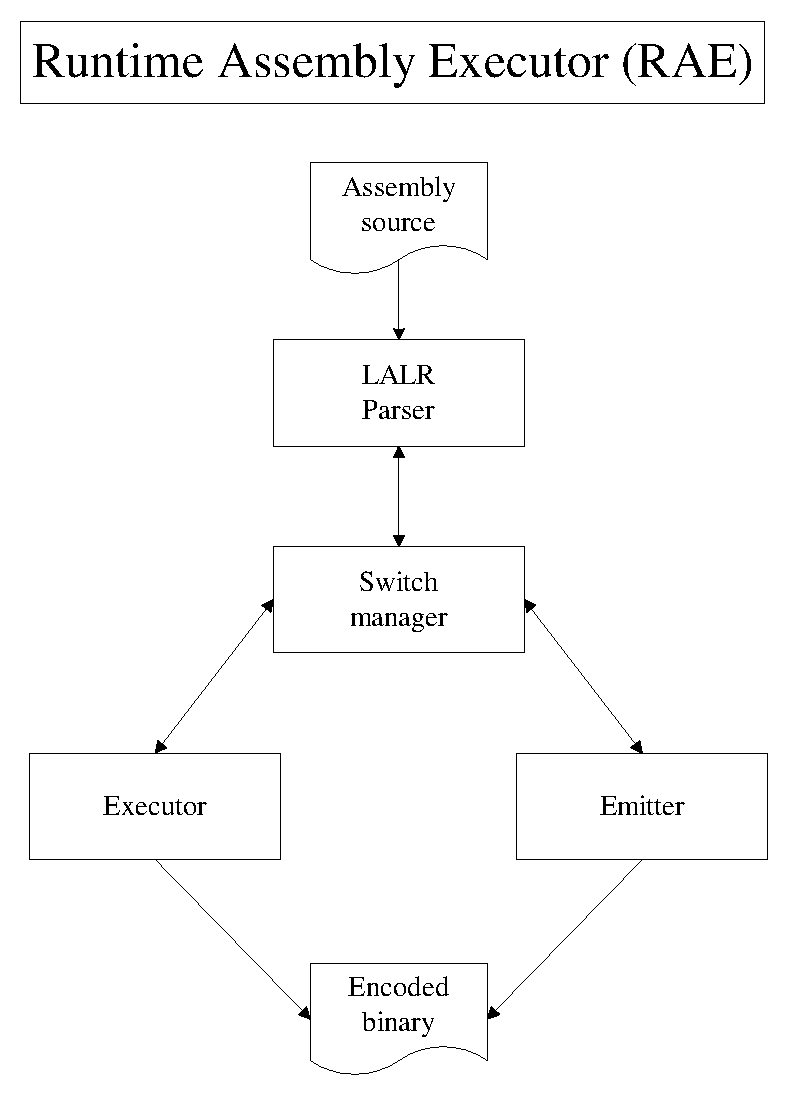
\includegraphics{figures/rae.eps}}
\centerfigend{fig-rae}{Components of RAE}

RAE is made up by 4 main components (see Figure~\ref{fig-rae}):  

\begin{itemize} 
\item 	The parser, 
		which parses VPO-generated assembly files using a LALR parser. 
		Structures, relocations, label information are gathered as each unit 
		of input is parsed.  Details regarding the parser are
		explained in more detail in the following subsections. 

\item 	The emitter, which uses NJMC toolkit encoding routines to encode the
		assembly instructions into binary instructions.  The emitter is invoked
		mainly by the parser and is reponsible for outputing the final binaries
		needed by the executor. 

\item 	The executor, which executes the translated binary code at run-time. 
	
\item 	The switch manager, which maintain the connections between the above
		components.  It jobs is to direct the flow of translation\/program 
		execution and the communications between the components such that 
		on-demand processing can be achieved.  
\end{itemize}

The dynamic behaviour of RAE results mainly from the ability to process
on-demand in the individual components.  Processing of each component are
done only when there is a need to do so.  For example, when the emitter
emits enough information for execution, the executor is invoked.  The
executor is then paused when there is a call to a label which it does not
yet know about, hence it invokes the parser to parse more source in search
for the desire label.  Each component are closely coupled in a way that
they are triggered on-demand.  Granularity of RAE can be seen as
processing one procedure at a time in the parser component. 


\section{RAE Parser} 
The parser is the first to be called by RAE.  
In a sequencial order, the parser starts at the top of the assembly file and
processes the input in an orderly fashion.  
The granularity unit of the parser is a single procedure at a time.  
The parser must gather enough information from the input file such that other
components can be invoked.  
During the parse, the parser invokes the emitter for every instruction that 
needs to be emitted.  
The combination of parsing and emitting pauses once the entry point to the 
main program is found in which the executor is called to execute the encoded
instructions.
Sometime during the running of the program, the switch manager may invoke the 
parser to parse more assembly input as needed.

Each procedure is consider to have a text segment and a local data segment.  
The first procedure
starting from the begining of the file and have no text segment.  It has a
single data segment which stores the labels that are accesible by the rest
of the program.  This is the only procedure that has no code segment and
it is the global data segment.  This segment is responsible to have names
and labels that are used throughout the rest of the program which are not
found in there local data segments.  Apart from being a single segment
procedure, this segment contains data that are similar to the rest of the
procedure's local data segments (at least in the eyes of the parser, they
are treated the same). 


\subsection{Data Segments} 

Data segments are static piece of memory that are allocated before the 
execution of the program.  
These segments may contains both initialised and uninitialised data.
Two types of data segments can be found in an assembly input file: 
texttt{global} and texttt{local} data segments.
The global data segment contains variables and label references that can be
accessed anywhere throughout the program.  
Contents within the local data segment are known only to its corresponding 
text segment.

\subsection *{Input to the parser}

The following assembly constructs are found in data segments within the input
file.

\begin{itemize} 
\item 	\texttt{.seg "data"} - this signifies the beginning of a data segment.
It is at this point that a new data relocatable block is created.  
Relocatable block are base structures provided by the NJMC toolkit. 

\item	\texttt{.align NUM} - NUM is usually 4, 8 or 16.  
a call to the align(NUM) routine is made whenever this is encoutered. 

\item	\texttt{.common VAR,SIZE,ALIGN} - variable VAR is declared with 
size SIZE, and its byte aligned to ALIGN.  
Call to align(ALIGN) is made first, VAR is added to the global symbol 
table if it have not been already added, SIZE bytes
is emited to the current relocatable block using emitm().  Since no
initial value is required, the emitter simply emits junk (currently set to
be the integer 2) for the .common identifier.  For example, in the
following variable declaration \\ \texttt{.common cm\_var, 1024, 4} \\ the
name \texttt{cm\_var} will be added to the symbol table with its offset
from the beggining of the global data segment.  The RAE then emits a
series of 1024 bytes with the value of 2 to specify that the address is
occupied through a series of calls to \texttt{emitm} (which handles
incrementing the \texttt{PC} counter and allocating space if the maximum
buffer space is reached). Another way to do this would be to call
\texttt{addlc()} which simply increments the \texttt{PC} counter. 
Although using \texttt{addlc()} is considerably quicker, extra code needs
to be added to performs similar housekeeping functions in \texttt{emitm}
like checking buffer overfloads if the relocatable block have just been
created.  addlc() can be safely used if a previous call the emitm() has
been made since the creation of the relocatable block.  If addlc() is the
first to be called after a new relocatable block, then some house keeping
is definately required. 

\item	\texttt{.global NAME} - signifies NAME is a global name that can 
be accessed anywhere in the program.  
NAME is added to the global symbol table and a
relocatable address for the NAME label is also created. 

\item	\texttt{LABEL:} - signifies a data label definition.  
If LABEL is not already in
the symols table (searches local symbols first then globals), it will be
added and a relocatable address is created aswell. 


The following belong within a LABEL 

\begin{itemize} 
\item .byte XXXX, 
\item .word XXXX, 
\item .double XXXX,
\item .ascii XXXX - the values XXXX associated with these tags are simply emited
to the current relocatable block. 
\end{itemize}

\end{itemize}

The input assembly file is generated from VPO, but its organisation
of data and text segments make it difficult for a single parse.  
For each text segment, there is always a corresponding local data segment 
(which could be empty).  
The organisation of the VPO assembly will start with the
global data segment, follow by the first text and local data segment pair,
then the second pair etc...  in that order.  Each pair of the text and
local segments is grouped as a single procedure by the parser.  Problem
with a single parse over the input file arises when encountering
references to local data variable its corresponding the text segment. 
Since its local data segment comes after its text segment, no reference
information about variables are known at the point of emiting an
instruction.  To overcome this problem, each local data segment could be
moved infront of its repectable text segment.  This can be very tedious
when the input file contains a large number of procedures.  To fixes this
problem, relocation closures are used.  Relocation closures are created
when an unknown symbol (or address) is referenced in the text segment. 
When the symbol is discovered (in its corresponding local segment), the
closure is applied to the instruction that created the relocation closure. 
This is done by patching the instruction space with the correct relocation
address. 

\subsection *{Example}

The following example code demonstrates the processing done during the
parse: 

input code:  
\begin{verbatim}
.seg "text"             (1)  
.align 8                (2)  
.global .L45            (3)  
.L45:                   (4) 
save %sp, -96, %sp      (5)  
sethi %hi(.L60), %o0    (6)  
add %o0, %lo(.L60), %o0 (7) 
...  
...  
.seg "data"             (8)  
.align 8                (9)  
.L60:                   (10)  
.word 0x46ff            (11)  
... 
\end{verbatim}

At the entry to the procedure, the parser allocates a new relocatable
block and does some housekeeping (1).  At (3), the symbol .L45 is added to
the global symbols table (global so that other procedures can call .L45). 
A label for .L45 is also created but not defined.  (4) defines label .L45
by assigning it the current offset from the beginning of the relocatable
block.  A save instruction is emited to the relocatable block by invoking
the respective emitter function (5).  As it encouters .L60 in (6), it
attempts to lookup the global symbols table in search for .L60 and fails. 
The parser adds .L60 to the local symbols table and creates a label for
it.  It then invokes the emitter which creates a relocation closure for
this instruction.  (7) uses .L60 again, this time the parser finds .L60 in
its local symbols and asks the emitter to emit the add instruction.  But
the emitter detects that .L60 is not defined and created another
relocation closure.  When the text segment is completed, the parser
creates another relocatable block for its local data segment(8).  At (10),
the parser defines .L60.  At (11), 0x46ff is emitted to the relocatable
block. 

As the RAE parser parses the VPO assembly output, it builds 2 (except the
first procedure) relocatable block for each procedure it encounters along
with a symbol table for all the symbols that are define in this procedure. 
When the parser finishes parsing a procedure, it tries to fix all the
incomplement instructions during the parse by applying the closures.  As
each closure is being appled, it patches over incomplete instruction with
the correct target address of the labels. 

Notice that the first procedure does not have a text segment.  This
procedure contains the global data section, hence the symbols table for
this procedure contains all the symbols and labels that are global to the
entire program.  This table defines variables that are accessible during
program execution. 

For succesful instruction encoding using global and local variable address
references and run-time execution, an exact copy of the disk image is
created in memory.  At the end of a procedure parse and after closures are
applied, information within each relocatable block are copied to a
contiguous piece of memory that is suitable for execution. 


\subsection{Text} 
As each procedure is being parsed, each assembly
instruction is determined, mapped and constructed by issuing a call to the
emmiter (see section 1.3) which invokes the corresponding NJMC encoding routine.  For example, for the assembly instruction 

\begin{verbatim}
	add %o0, 10, %o0 
\end{verbatim}

A call to the \texttt{add} function is made by the emitter to emit the
actual instruction to the text relocatable block. 

To process procedure call instructions, the parser looks up the global
symbol table and decides the next set of actions:  \begin{itemize} \item
For labels (infact, symbols as well) that are defined in the symbols
table, an explicit call instruction to the label's address is encoded. 
\item For labels not found in the table, the parser checks if the label
	exists in the libraries used by the program (currently only
	\texttt{libc.so.1} is checked). 
	If so, it is implemented as an indirected call.  Indirected calls
	are patched with two instructions---\texttt{sethi} and
\texttt{jmpl}. 
	The former instruction takes the address of the library routine,
	puts it into register \texttt{\%g5}, then a jump and link
(\texttt{jmpl})
	follows.  \item For unknown label, a call to the switch manager is
made.  The parser creates a new label for the destination of the call. 
Since the address of the destination is unknown at the time of encoding,
the
	name of the procedure that's being called is also passed to the
	switch manager. 
	See the section in On-demand to see how the switch manager is
used. \end{itemize}

The processing of branches is similar to that of calls for labels that
have been defined.  Branch targets that are unknown will result in
generating a relocation closure for the instruction with the target label
added to the local symbols table.  Branch target is never in the
libraries.

Closures are applied at the end of the parsing phase.  All fix ups within
intructions are handled by looping through the set of closures and
applying each in turn.  For address that are still undetermined during
closure analysis, the program will simply fail with an error.


\subsection{Others} In the case of loads and stores during the parsing of
the input file, the parser needs to indentify and encode the appropriate
instructions. Both version of float and integer loads uses the same
\texttt{ld} mnemonic but their opcodes are different.  The parser
determines whether the instruction involves floating point registers and
encodes the instruction accordingly---\texttt{ld} for integer loads and
\texttt{ldf} for floating point loads.


\section{RAE emitter} The RAE's emitter is automatically generated by the
NJMC tookit using the Sparc encoding specifications.  Communication
between the parser and the emitter is through the functions found in
\texttt{sparc.h}.  This file provides encoding functions that will
produces machine binaries for each Sparc instruction. 


\subsection{NJMC toolkit}

The NJMC toolkit can use a machine instruction specification to create
both encoding and decoding routine.  In this report, I will be discussing
encoding only.  The routines that can be used for encoding (as are used in
RAE) are generated by running xtools over the Sparc specification files. 
Function names are generated with relation to the names used in the spec
files.  eg. the add instruction will be implemented with the C function
ADD(rs1, reg\_or\_imm, rs2). 


\section{RAE executor} Control is parsed to the RAE executor with the
entry address of the main program.  The executor executed the encoded
instruction just like any other piece of code in memory.  The name of
executor is gcode, and its assign a value when the address of main is
found.  The executor is invoke by calling gcode() explicitly. 


\section{On-demand} One significant change from RAE rev 1 to rev 2 is the
introduction of on-demand processing.  On-demand processing allows
parsing, emiting and executing of code that are only requied at run-time. 

For each procedure parsed by the RAE parser, 2 relocatable blocks and 1
symbols table is constructed (except the first procedure).  The emitter is
invoked during the parse and actual instructions and data are emited
within the relocatable block.  At the end of a parse (end of one
procedure), all the relocation closures are apply.  Copies of each
relocatable to a contiguous piece of memory is done before the RAE parser
starts parsing another procedure. 

The RAE parser will parse the input file until the main procedure is
found.  Program execution start as soon as main is parsed and emited.  For
all other piece of code that are not yet parsed at this point in time, a
call to the "switch manager" is generated to take its place.  When a
program needs to call a procedure "proc1" yet to be parsed, instead it
calls the switch manager.  The switch manager looks up the list of
procedure that it knows about and tries to find "proc1".  If sucessful,
"proc1" is called.  If "proc1" does not exist in the known procedure list,
the switch manager asks the parser to parse another procedure until
"proc1"  is found and the code is emited.  When "proc1" is found, the
switch manager no only passes control to "proc1", it also patches the
original call to the switch manager with a call to "proc1". 

Example code before and after patching. 

original code to from input

\begin{verbatim}
add %o0, 0x188, %o0 
call proc1, 2 
add %o1, 0x302, %o1
\end{verbatim}

When call to "proc1" needs to be emited, the emitter emits a call to the
switch manager instead (instructions 0x60a70 and 0x60a74).  In order for
the switch manager to know that "proc1" is the required procedure, the
address containing the string "proc1" is also emited (instructions 0x60a68
and 0x60a6c). 

\begin{verbatim}
0x60a64 <_end+32108>:  add %o0, 0x188, %o0 
0x60a68 <_end+32112>:  sethi %hi(0x5bc00), %g5 
0x60a6c <_end+32116>:  add %g5, 0x258, %g5      ! 0x5be58 <_end+12640> 
0x60a70 <_end+32120>:  sethi %hi(0x13c00), %g6 
0x60a74 <_end+32124>:  call %g6 + 0x3b4         ! 0x13fb4 <switch_manager>
0x60a78 <_end+32128>:  add %o1, 0x302, %o1
\end{verbatim}

After the switch manager have found the address for "proc1" (through calls
to the parser and emitter in search for "proc1"), it patches the call to
the switch manager with a straight call to "proc1".  It also removes the
instructions at 0x60a68 and 0x60a6c. 

\begin{verbatim}
0x60a64 <_end+32108>:  add %o0, 0x188, %o0 
0x60a68 <_end+32112>:  nop
0x60a6c <_end+32116>:  nop 
0x60a70 <_end+32120>:  sethi %hi(0x62000), %g5
0x60a74 <_end+32124>:  call %g5 + 0x390 		! 0x62390 <_end+38552> 
0x60a78 <_end+32128>:  add %o1, 0x302, %o1
\end{verbatim}

Because the switch manager is do self modifying code, flush instructions
is needed to flush the cache such that it reflect what is now in memory. 
A jump to the procedure "proc1" is made at the end of the switch manage
			 % assembler encoder using the NJMCTK 


\part{Results}
\label{part-results}

	
\chapter{Results}
\label{ch-results}

{\small
\begin{flushright}
Documentation: Cristina, Mike [Sep 99]
\end{flushright}
}

This chapter provides current preliminary results in the use of
the \uqbt\ framework in 5 instantiations of the framework. 
The results were reported in 1999 at the Workshop on 
Binary Translation, Oct 99, and have not been updated since. 

After these results were reported, there has been progress
such that all the SPARC to SPARC and Pentium to SPARC tests in
the distribution file \texttt{test/regression.test} pass. Note 
that some of these passes are in fact rather forced---in some 
cases the generated C code is edited with a sed script. 
These are all due to limitations that we acknowledge, and which 
could be fixed if and when some things get implemented, such as 
endianness analysis for library function parameters. Of the Spec95 
integer benchmarks, only \texttt{compress} and \texttt{go} actually 
translate correctly, as far as we know, and only \texttt{compress} 
translates Pentium to SPARC. We have attempted to translate a few others, 
but it's tedious work due to lack of better debugging infrastructure. 
This illustrates the need for a debugging system, as discussed
elsewhere.

The following translators were used for experimentation and 
data collection: 

\begin{itemize}
\item uqbtss: static SPARC to SPARC
\item uqbtsp: static SPARC to Pentium
\item uqbtps: static Pentium to SPARC
\item uqbtpp: static Pentium to Pentium
\item uqbtsj: static SPARC to Java bytecode
\end{itemize}

A SPARC to SPARC and a Pentium to Pentium translators are useful
to test the adequacy of the internal representation, as translated
programs should not slow down when translating from machine M to 
machine M using the same optimizer compiler.  
Further, as seen in the results in this section, a binary translator 
can be used as an optimizer of binary code.  

The UQBT framework currently decodes and partially analyzes 
SPEC95 benchmark programs, such as compress, ijpeg, and gcc.
The largest of such programs is gcc with 1Mb of binary code (1.6Mb 
executable on SPARC and 1.2Mb on Pentium).
Our type analysis implementation is not complete, therefore we
currently only translate programs that take integer and pointer to
data parameters.
This limits the size of the programs that can currently be translated 
to the ones presented in Figure~\ref{fig-results}.
Further, our resourceable interpreter is not fully implemented yet,
hence we do not support programs that require runtime interpretation.
This has not been a problem for the programs presented herein, but
will be required for larger programs.

\begin{figure*}[htp]
{\small
\begin{minipage}[b]{\linewidth}
\begin{center}
\begin{tabular}{|r|r|r|r|r|} \hline
        & \multicolumn{2}{c|}{Translated Code} &
        \multicolumn{2}{c|}{Native Code} \\
Program & gcc opt & cc opt & -O0 & -O4 \\ \hline
Fibo(40) sec & 18.2  & 21.3 & 41.0  & 23.0 \\
       bytes & 24,924  & 6,700 & 24,628 & 24,564 \\ \hline
Sieve(3000) sec & 23.7 & 24.1 & 29.3 & 24.5 \\
       bytes & 24,732 & 6,316 & 24,552 & 24,452 \\ \hline
Mbanner(500K) sec & 25.8 & 22.2 & 63.7 & 26.6\\
       bytes & 30,500 & 12,248 & 30,652 & 30,268 \\ \hline
\end{tabular}
\end{center}
%\vspace*{0.1cm} 
\center{Static SPARC to SPARC Translation}
\end{minipage}\hfill
\vspace*{0.4cm}

\begin{minipage}[b]{\linewidth}
\begin{center}
\begin{tabular}{|r|r|r|r|r|} \hline
        & \multicolumn{2}{c|}{Translated Code} &
        \multicolumn{2}{c|}{Native Code} \\
Program & gcc opt & cc opt & -O0 & -O4 \\ \hline
Fibo(40) sec & 23.0 & 24.3 & 41.0 & 23.0 \\
       bytes & 24,916 & 6,680 & 24,628 & 24,564 \\ \hline
Sieve(3000) sec & 26.9 & 23.9 & 29.3 & 24.5 \\
       bytes & 24,776 & 6,312 & 24,552 & 24,452 \\ \hline
Mbanner(500K) sec & 53.3 & 36.9 & 63.7 & 26.6 \\
       bytes & 34,188 & 21,448 & 30,652 & 30,268 \\ \hline
\end{tabular}
\end{center}
%\vspace*{0.1cm} 
\center{Static Pentium to SPARC Translation}
\end{minipage}\hfill
\vspace*{0.4cm}

\begin{minipage}[b]{\linewidth}
\begin{center}
\begin{tabular}{|r|r|r|r|r|} \hline
        & \multicolumn{2}{c|}{Translated Code} &
        \multicolumn{2}{c|}{Native Code} \\
Program & gcc opt & cc opt & -O0 & -O4 \\ \hline
Fibo(40) sec & 27.7 & 28.5 & 28.6 & 25.9 \\
       bytes & 16,512 & 7,292 & 16,144 & 16,152 \\ \hline
Sieve(3000) sec & 17.8 & 17.4 & 18.9 & 18.6 \\
       bytes & 16,244 & 6,548 & 15,964 & 15,944 \\ \hline
Mbanner(500K) sec & 42.5 & n/a & 80.5 & 44.8 \\
       bytes & 22,240 & & 21,524 & 25,436 \\ \hline
%~\footnote{4,096 bytes added to executable to adjust data page size} \\ \hline
\end{tabular}
\end{center}
%\vspace*{0.1cm} 
\center{Static SPARC to Pentium Translation}
\end{minipage}\hfill
\vspace*{0.4cm}

\begin{minipage}[b]{\linewidth}
\begin{center}
\begin{tabular}{|r|r|r|r|r|} \hline
        & \multicolumn{2}{c|}{Translated Code} &
        \multicolumn{2}{c|}{Native Code} \\
Program & gcc opt & cc opt & -O0 & -O4 \\ \hline
Fibo(40) sec & 25.8 & 24.5 & 28.6 & 25.9 \\
       bytes & 16,496 & 7,268 & 16,144 & 16,152 \\ \hline
Sieve(3000) sec & 18.6 & 17.1 & 18.9 & 18.6 \\
       bytes & 16,228 & 6,536 & 15,964 & 15,944 \\ \hline
Mbanner(500K) sec & 48.7 & 46.5 & 80.5 & 44.8 \\
       bytes & 25,664 & 16,016 & 21,524 & 25,436 \\ \hline
%~\footnote{4,096 bytes added to executable to adjust data page size} \\ \hline
\end{tabular}
\end{center}
%\vspace*{0.1cm} 
\center{Static Pentium to Pentium Translation}
\end{minipage}\hfill
\vspace*{0.4cm}

%\begin{minipage}[b]{.46\linewidth}
%\begin{tabular}{|r|r|r|r|} \hline
%        & \multicolumn{1}{c|}{Generated Code} & 
%	\multicolumn{2}{c|}{Native Code} \\ 
%Program & Total & -O0 & -O4 \\ \hline
%Fibo(40) sec & 179.27 & 41.0 & 23.0 \\
%	byte & & 24,628 & 24,565 \\ \hline 
%Sieve(3000) sec & 83.00 & 29.3 & 24.5 \\
%	byte & & 24,552 & 24,452 \\ \hline 
%Mbanner(500K) sec & & & \\ 
%	byte & & & \\ \hline
%\end{tabular}
%\vspace*{0.1cm} \center{Dynamic SPARC to SPARC Translation}
%\end{minipage}\hfill
%\begin{minipage}[b]{.50\linewidth}
%\begin{tabular}{|r|r|r|r|r|r|} \hline
%        & \multicolumn{3}{c|}{Translated Code} & 
%        \multicolumn{2}{c|}{Native Code} \\
%Program & startup & dispatch & gen code & -O0 & -O4 \\ \hline
%Fibo(40) sec & 0.48 & 0.03 & 191.39 & 41.0 & 23.0 \\
%        bytes & & & 1,208 & 24,628 & 24,564 \\ \hline
%Sieve(3000) sec & 0.52 & 0.08 & 80.85 & 29.3 & 24.5 \\
%        bytes & & & 1,556 & 24,552 & 24,452 \\ \hline
%Mbanner(500K) sec & & & & & \\
%        bytes & & & & & \\ \hline
%\end{tabular}
%\vspace*{0.1cm} \center{Dynamic Pentium to SPARC Translation}
%\end{minipage}\hfill
%\vspace*{0.4cm}
%
%\begin{minipage}[b]{.42\linewidth}
\begin{minipage}[b]{\linewidth}
\begin{center}
\begin{tabular}{|r|r|r|r|r|} \hline
        & \multicolumn{2}{c|}{Translated Code} & 
        \multicolumn{2}{c|}{Native Code} \\
Program & Interpreter & JIT & -O0 & -O4 \\ \hline
Fibo(40) sec & 421.64 & 58.02 & 41.0 & 23.0 \\  
	bytes & 739 & 739 & 24,628 & 24,565 \\ \hline  
Sieve(3000) sec & 103.66 & 20.52 & 29.3 & 24.5 \\ 
	bytes & 677 & 677 & 24,552 & 24,452 \\ \hline
%Mbanner(500K) sec & & 10m16.06 & 22.11 & 10.01 \\ 
% 	bytes & & & & \\ \hline
\end{tabular}
\end{center}
%\vspace*{0.1cm} 
\center{Static SPARC to Java Bytecode Translation}
\end{minipage}\hfill
%\begin{minipage}[b]{.46\linewidth}
%\begin{tabular}{|r|r|r|r|r|} \hline
%         & \multicolumn{2}{c|}{Generated Code} & 
%         \multicolumn{2}{c|}{Native Code} \\
%Program & interpreted & JIT & -O0 & -O4 \\ \hline
%Fibo(40) sec & & & & \\  
% 	bytes & & & & \\ \hline  
%Sieve(3000) sec & & & & \\
% 	bytes & & & &  \\ \hline
%MBanner(500K) sec & & & & \\ 
% 	bytes & & & & \\ \hline
%\end{tabular}
%\vspace*{0.1cm} \center{Static Pentium to Java Bytecode Translation}
%\end{minipage}\hfill

\label{fig-results} \caption{Running Times and Code Sizes for Static
	Translators Instantiated from the UQBT Framework}
}
\end{figure*}

%%Figure~\ref{fig-results} presents results for 6 different
%%Figure~7 presents results for 5 different instantiations of the UQBT 
Figure~\ref{fig-results} presents results for 5 different instantiations of 
the UQBT framework.  The test programs are: 

\begin{itemize}
\item Fibo(40), which calculates the fibonacci of 40 and has 63 lines 
of assembly code, 
\item Sieve(3000), which calculates the first 3000 primes and has 
61 lines of assembly code, and
\item Mbanner(500K), a modified version of banner(1), which loops 
500,000 times to display argv[1] (``1234567890'' in this case) and 
has 204 lines of assembly code and a read-only data section 
of 336 bytes.
\end{itemize}

For all programs, we measured the time in seconds to execute
the program on the target machine and compared that to the
time measurement produced by a native compiler on that target
machine; this allows us to see the quality of the translation.
Each test program also lists on the second row the size in bytes
of the executable file for comparison purposes.
SPARC results were obtained on an UltraSPARC II, 250MHz machine
with 320Mb RAM running Solaris 2.6.
Pentium results were obtained on a Pentium MMX, 250 MHz machine
with 128Mb RAM running Solaris 2.6.
The source binary programs (input to the translator) were all compiled 
with gcc 2.8.1 -O4.  
Translated code programs used two different optimizing C 
compilers; gcc 2.8.1 and cc 4.2, on both SPARC and Pentium machines. 
Native code for the target machine was compiled using gcc 2.8.1
with -O0 and -O4 options, on both SPARC and Pentium.  
%%Results for -O0 are included to indicate how much variation optimization 
%%causes on the source architecture. 

As can be seen from the results, the statically translated code is just 
as efficient as native code on translations across the same 
architecture (i.e. SPARC to SPARC and Pentium to Pentium), 
and small or negligible overhead is created on static register-based
translations across different architecture machines.
This is due to the abstraction of code into \hrtl\ code 
and perhaps the small size of the test programs, which do not 
necessarily test all the features of large programs 
(such as differences in types or the need for interpretation).
Some translated programs (those translated by uqbtss and uqbtpp) are 
faster than their native counterparts because of accidents of instruction 
scheduling.  We compared the input and the translated program and 
noticed a few extra nop's and unfilled delay slots in the input 
optimized binaries.  These can make a very large difference for 
programs like fibonacci, which have very short inner loops doing most of 
the work.

The version of Sieve that is translated from the Pentium to the 
SPARC runs 9\% slower than the version compiled from C source 
code by the native SPARC compiler, when using gcc as the optimizer 
with UQBT. Because the Pentium has fewer registers than SPARC, 
the Pentium compiler did not put all variables in registers. 
In the translation from the Pentium binary, those variables remain
in memory, but when the native SPARC compiler translates the same
source code, it puts all variables in registers, so the natively 
compiled version is 9\% faster.  In contrast, the cc optimizer does  
perform this optimization and the result is a generated binary 
that runs at the same speed as native code.  

Translations between machines of different endianness, such as 
SPARC and Pentium, may require the use of byte swapping at each load 
and store in order to access initialized data.  This is the case
of the Mbanner Pentium to SPARC static translation, where a 100\%
overhead is seen.  
This is due to two main factors: memory locations are not promoted 
to registers wherever possible, and there are redundant byte swaps 
due to endianness differences.
In our translation to SPARC, the machine has to 
perform costly byte swapping for one 32-bit load instruction, which 
results in 10 SPARC instructions.  
Two redundant 32-bit byte swaps result in 20 SPARC instructions 
which the optimizer cannot remove.  This problem is not seen in 
SPARC to Pentium static translations however, because the Pentium has 
a single instruction to perform 32-bit byte swapping. 
The two shortcomings identified in the generated code can be 
rectified by implementing binary translation-specific optimizations 
at the \hrtl\ level, before emitting machine-dependent code.  

The Pentium to SPARC translations suffer a large performance hit
because of the way that endianness swaps are implemented. The
cost is some 8 SPARC instructions, with an extra 2 for the first
one (and if the register used to hold the mask is re-used). Most
SPARC machines these days have UltraSparc processors, and with
these machines it is possible to perform endianness swaps during
loads and stores (alternate address space 0x88 performs the
required swapping).

To implement the alternate address scheme, the macros need to be
split into two groups; one for loads, and one for stores. (Both
of these would be almost the same for Pentium targets). Also,
there is the issue that for the lowest overhead, two different
assembly language forms have to be used; one for when the SPARC
addressing mode is register plus register, and one for when it is
register plus constant. We did not implement these changes, 
so regrettably we do not know what the true cost of translation
from Pentium to SPARC really is (i.e. at present, it is
needlessly being swamped by the cost of endianness swaps using the 
first-mentioned method).

For the translator of SPARC to Java bytecodes we show 
initial results obtained without having performed stack-based 
optimizations on the code.  
Nevertheless, the JIT compiled 
version compares favourably with native code on the SPARC, 
especially due to the efficiency of present JIT compilers, 
which translate two or three bytecode instruction sequences 
into one target native instruction. 
These results apply to small integer benchmarks. 

      % results on performance of gen'd binaries

	
\chapter{Instantiation of Translators}
\label{ch-instantiation} 

{\small
\begin{flushright}
Design: Cristina; Documentation: Cristina [Apr 01]
\end{flushright}
}


This document is based on the experience gained by the 
UQBT team in instantiating binary translators out of the UQBT framework.  
The following translators have served as test beds for the 
development of this process: 

\begin{itemize}
\item SPARC to Pentium
\item Pentium to SPARC
\item MC68000 to MC68000
\item PA-RISC to SPARC 
\end{itemize}

The UQBT framework, described in Chapter~\ref{ch-uqbt-framework} 
and replicated below in Figure~\ref{fig-uqbt-framework}, provides 
the basis for a step-wise process of instantiating modules out of
the framework.  

\psfigbegin{figures/uqbtImplementation.eps}{10cm}
\psfigend{fig-uqbt-framework}{The UQBT Framework}

In order to instantiate a new translator, the APIs and specification 
files for the source platform need to be described. 
The output of the module that services each API or specification is 
tested in order to ensure correctness of the intermediate output.  

The instantiation process consists of the following steps: 
\begin{enumerate}
\item Binary-file decoder support

\item Instruction decoding support 

\item Instruction semantics support

\item Control transfer support

\item Procedural abstraction support

\item Machine-specific support

\item Code generation support
\end{enumerate}

Each step is described in some detail in the following sections.
Throughout this presentation, the steps have been divided into 
the three logical parts of the translator, that is, instantiating
a front-end, instantiating to HRTL level, and instantiating
a back-end.


\section{Instantiating a New Front-end}
In order to support a new front-end for a machine M$_s$, we 
need to provide support for the binary-file format in which 
the executable file is stored in, as well as the syntax and 
semantics of the machine M$_s$ instructions.  

\subsection{Binary-file Decoder Support}
In order to support different binary-file formats, such as 
ELF, PE, PRC, etc, UQBT exports a loader API called 
\texttt{BinaryFile}.  \texttt{BinaryFile} is an abstract class 
that makes available functions to:

\begin{itemize}
\item construct, load and unload binary files, 
\item extract information from sections, 
\item extract information from symbol tables (if any), 
\item extract information from relocation tables (if any),
\item display/dump the contents of all headers, and 
\item obtain initial program state information, such as entry 
	point(s), and determine whether a given address is a dynamically-linked 
	address or not.  
\end{itemize}

For a given binary-file format BFF$_i$, the \texttt{BinaryFile} 
API is satisfied by implementing the derived BFF$_i$BinaryFile 
class.  In this class, some extra functions are used to 
implement the \texttt{BinaryFile} interface, depending on 
the complexity of implementing the API functionality.  

Testing of this step is done by displaying/dumping to the screen 
the contents of all headers and sections read from the file. 
This contents is then checked manually against the contents 
produced by a binary-file dump tool, commonly distributed with
operating systems these days.  For example, under Unix, the  
\texttt{elfdump} tool displays the contents of an ELF's file 
headers.  A typical size of information dumped is around 500 
lines of ascii text.  Similar results are achieved by using 
GNU's \texttt{objdump} tool. 

Modules to bring across from the UQBT source code (we use the
following command: \texttt{cvs co -N -d . uqbt/dirName} 
and then rename the \texttt{uqbt} directory to a suitable 
name): 
\begin{itemize}
\item The \texttt{uqbt/loader} directory and all its files
\item The \texttt{uqbt/include} directory and all its files
\item The driver and Makefile for the bffDump program 
	(\texttt{uqbt/loader/bffDump}); these programs 
	need to be placed at top level. 
\end{itemize}

The skeleton file \texttt{bffDump.cc} provides the basis 
for creating a binary-file dumper, also known by others as object 
dumper, which displays the raw contents of each of the headers and 
fields of the given binary-file.

The \texttt{BinaryFile::DisplayDetails} function needs to be overridden 
and implement the displaying of the BFF's header, its program 
header and section headers, as well as the information within 
those sections. 

Using \texttt{elfdump} on Solaris, the following options 
show parts of the Elf file; invoking \texttt{elfdump} with 
a file name displays all the section information in the file. 
Options (from the man page): 
\begin{itemize}
\item \texttt{-e}: dump the elf header,
\item \texttt{-p}: dump the program headers, 
\item \texttt{-c}: dump section header information,
\item \texttt{-d}: dump the contents of the .dynamic section,
\item \texttt{-s}: dump the contents of the symbol table sections (that
           is, .dynsym and/or .symtab).
\end{itemize}

Testing against a tool like \texttt{objdump} requires different
options to be set in order to see different parts of the file: 
\begin{itemize}
\item \texttt{--file-headers}: displays the Elf header
\item \texttt{--section-headers}: displays the section headers 
\item \texttt{--headers}: displays the section headers only (it 
	does not include the program headers)
\item \texttt{--syms}: displays the contents of the symbol table
\item \texttt{--dynamic-syms}: displays the contents of the dynamic symbol 
	table
\item \texttt{--all-headers}: displays all section headers and the 
	contents of the symbol table.
\end{itemize}


\subsection{Instruction Decoding Support}
	This is the most time consuming step in the process as the 
	binary translator writer needs to become fully familiar with 
	the instruction set to be supported.  This step involves 
	reading through architecture manuals and representing the 
	information for instructions in terms of the SLED language. 
	SLED allows for the description of the types of instructions 
	in a given machine, the fields of such instructions, the 
	values of particular fields of instructions, and the description
	of what individual instructions are, in essence, allowing for
	the mapping of binary bit streams to assembler instructions. 
	In our experience, depending on how complex the instruction 
	set is, and how familiar the writer is with the instruction 
	set, this step can take anywhere from 2 weeks to 2 months. 

    The New Jersey Machine Code toolkit (NJMCTK) not only supports 
	the SLED language, but also supports an abstraction to decode and 
	encode machine instructions.  The decoding abstraction provides for
    a \emph{matching} statement whose syntax resembles that of
    a C switch statement, and whose semantics is equivalent to
    matching the series of bits that form an instruction and
    returning the values of the variable fields of an instruction.
    In this way, a decoder (disassembler) of machine instructions 
	can be written, and the time to do this is minimal (less than 
	1 day), in fact, it is possible to automatically generate such
	a decoder.  This decoder is tested against an existing 
	disassembler for the source machine through a series of test 
	cases.  This is possible as most Unix systems include a \emph{dis} 
	utility in their distribution or one is included as part of 
	the GNU \emph{binutils}.

The following files/directories need to be downloaded: 
\begin{itemize}
\item \texttt{uqbt/loader}
\item \texttt{uqbt/include}
\item \texttt{uqbt/machine}
\item \texttt{uqbt/disasm} and put the files 
	from this directory at top level (disasm.cc, disassembler.m, mltk.sh 
	and Makefile)
\item rename directory \texttt{uqbt} to something else (e.g.
	\texttt{disasm})
\end{itemize}

Write the SLED spec for the architecture of choice.  
New machine descriptions are to be placed in the 
\texttt{machine/machineName} directory. 
Write a decoder based on the spec; sample decoders are given 
in the machine directory; for example, the 
\texttt{machine/sparc/disassembler.m} 
file is the decoder for the SPARC. 

The decoder to be written is a ``matching'' file, which gets 
processed by the New Jersey Machine Code toolkit (NJMCTK), along
with the SLED spec, into a C++ file which performs the matching
of bits to instructions.  
For information on SLED specifications refer to Ramsey and 
Fern\'{a}ndez~\cite{Rams97} and Chapter~\ref{ch-decoding} of 
this documentation.  

Appendix~\ref{ch-config} contains notes on how to configure
UQBT to generate disassemblers. 


\subsection{Instruction Semantics Support}
	The writing of the SSL spec is not too hard to do once the 
	SLED spec has been written, basically because by then the 
	writer is very familiar with the instruction set being 
	described.  In our experience, writing the SSL spec takes 
	less than one third of the time that it takes to write the
	SLED spec.  

	Our current testing of the SSL spec is in terms of an extension
	to the decoder.  Instead of the decoder dumping raw assembly 
	information, it dumps RTL information.  Such information is 
	manually tested against the assembly output. 

In the decoder file, you need to add support to return semantic
strings rather than plain strings.  Further, an extra function 
will be needed to cater with numbers and predefined register 
names (e.g. dis\_Reg() and dis\_Num()). 

Except for the PA-RISC, all other CISC and RISC architectures we have 
dealt with were almost straight forward supported by SSL.  However, 
in the case of PA-RISC, a more expressive language was needed in order 
to support pre and post semantics of instructions based on bits of 
an instruction.  This mean that an extension to the language was 
done and it took far longer than expected.   


\section{Instantiating to HRTL Level}
The M$_s$-RTL to \hrtl\ translator is composed of support for 
control transfer instructions, procedural information, and 
any extra code to support source machine-specific details. 

\subsection{Control Transfer Support}
	The New Jersey Machine Code toolkit (NJMCTK) supports the 
	SLED language as well as an abstraction to decode and encode 
	machine instructions.  The decoding abstraction provides for 
	a \emph{matching} statement whose syntax resembles that of 
	a C switch statement, and whose semantics is equivalent to 
	matching the series of bits that form an instruction and 
	returning the values of the variable fields of an instruction.
	In this way, a decoder of machine instructions can be written. 
	The support for the control transfer API is in terms of 
	extra instructions that get added to this matching driver 
	statement, so that control transfer information gets 
	encoded into the decoded $M_s$-RTLs.    	

	This API is very loose and not formally specified per se, 
	though it is hardcoded into the code.  The M$_s$-RTL instructions
	to which control transfer support has been applied, are an 
	``in between'' RTL form that we call IRTL.  IRTL stands for 
	``independent RTL'', and they resemble HRTL instructions, 
	with the exception that their operands have not been obtained 
	yet (these are obtained through procedural abstraction 
	recovery). 

	This step is almost trivial and can be implemented in 1 day 
	after looking at skeletons of existing translators. 

\subsection{Procedural Abstraction Support}
    The PAL spec is based on the operating system ABI conventions
    for setting up the call stack frame, parameter passing and
    calling conventions.  Specifying this information takes
    little time (2 days) once the information to be specified has
    been determined.  

    Testing of the PAL spec is done by compilation into the
    source binary form.  In this way, a translator of mc68328 Palm
    to mc68328 Palm binaries is instantiated for testing purposes.
    We test the SSL and PAL specs by determining if the translated
    programs behave in the same way as the original program.
    In our experience, we do not introduce performance degradation,
    in fact, the generated binaries compare favourably to native
    code geneated on the target machine, and in some cases it
    performs faster (due to optimization choices).  However, before
	being able to perform this test, the next step may need to 
	be applied. 

	Programs do not necessarily only adhere to the OS' ABI calling 
	conventions, therefore, some of the calling conventions that 
	we have included in PAL specs have been determined by trail and 
	error, after testing a program that does not adhere to the 
	ABI conventions.  We normally just include the new convention in
	the PAL spec. 

\subsection{Machine-specific Support}
	Add any extra analysis that is too machine-specific: 
	In order to remove all the peculiarities of a given source 
	machine, there may be need for an extra analysis to be added. 

	In our experience, each machine has a particular peculiarity 
	that is too machine-specific to be supported in the framework. 
	For example, SPARC has delayed transfers of control, x86 has 
	a stack-based representation for their floating point instructions, 
	mc68k makes use of a data pointer as a global pointer into data, 
	etc.  We normally try to address these issues in a fairly 
	generic way, though it is not always necessary to solve them 
	in that way.  In the case of delayed transfers of control, our 
	generic solution has been useful for reusing it for PA-RISC 
	code.  


\section{Instantiating a New Back-end}
Throughout the last few years, the UQBT's back-end has interfaced 
to a C compiler in order to optimize the intermediate code 
generated by UQBT.  In that framework, HRTL code is translated
to low-level C code, effectively using the C compiler as an 
assembler.  
We are now extending the framework to integrate with existing 
retargetable optimizers at the RTL level.  In this way, HRTL 
code is translated to $M_t$-RTL code and fed into an optimizer
such as VPO~\cite{Beni88} using the new VPO interfaces from the
Zephyr project~\cite{Vpo98}.  
Figure~\ref{fig-newUqbt} illustrates the new UQBT framework.  

\psfigbegin{figures/uqbtOverall2001.eps}{10cm}
\psfigend{fig-newUqbt}{The 2001 UQBT Framework}

In order to generate $M_t$-RTL code we need to solve several 
problems that are not discussed in this paper; these are: 
\begin{itemize}
\item Transform HRTL code to $M_t$-RTL code in a machine-independent way. 
      This step requires a few extensions to the PAL language in 
      order to support code generation of procedure call information 
      in a retargetable way, for example, by being able to use 
      specified calling conventions and parameter passing conventions, 
      as well as being able to set up the stack frame in the way expected
      in the target machine. 

\item Satisfy the $M_t$-RTL invariant that some optimizers require. 
      This invariant basically asks for an RTL to be equivalent to 
      an assembly instruction in the target machine.  This invariant 
      allows retargetable optimizers to perform not only machine-independent 
      optimizations but also machine-dependent ones. 
\end{itemize}


\subsection*{Translation via low-level C}
The C code generator back-end generates low-level C code, effectively
using the C language as a macro assembler.  Figure~\ref{fig-cgen-eg} 
shows the code generated by this back-end for the sample program. 
As can be seen from the code, type casting is used very often  
due to the need to ensure that the C compiler does not infer different
semantics to the one expected.  

\centerfigbegin
\begin{fnverbatim}
#include "uqbt.h"
void proc1(int16 v0, int32 v1, int16 v2) {
	int16 v3;
	int32 v4;
	int16 v5;
	int16 v6;
	int16 v7;
	int16 v8;
	int32 r3, r4, r5, r8;
	int32 temp1;
	int32 tmp1;
	/* 3c6 */

	*(int16*)&r5=v0;
	*(int16*)&r4=v2;
	temp1= *(int16*)&r4;
	v5=temp1;
	v4=33566720;
	v3=proc3(v4,v5);
	temp1=v3;
	*(int16*)&r3=temp1;
	tmp1=(unsigned int16)( *(unsigned int16*)&r3);
	v6=tmp1;
	if ((*(int32*)&v6)==(0)) goto L1;
	temp1=(int32)( *(int16*)&r3);
	r8=temp1;
	temp1=r8;
	*(int32*)&v3=temp1;
	goto L2;
L1:		/* 3f0 */
	temp1= *(int16*)&r5;
	v3=temp1;
	v7=v3;
	if ((*(int32*)&v7)==(0)) goto L3;
	goto L4;
L3:		/* 3f6 */
	v3=proc2();
	temp1=v3;
	 *(int16*)&r3=temp1;
	tmp1=(unsigned int16)( *(unsigned int16*)&r3);
	v8=tmp1;
	if ((*(int32*)&v8)==(0)) goto L5;
	temp1=(int32)( *(int16*)&r3);
	r8=temp1;
	temp1=r8;
	*(int32*)&v3=temp1;
	goto L2;
L5:		/* 406 */
	v5=1000;
	FrmGotoForm(v5);
	proc4();
	proc5();
L4:		/* 418 */
	*(int32*)&v3=0;
L2:		/* 41a */
	return;
}
\end{fnverbatim}
\centerfigend{fig-cgen-eg}{Generated C code for the example in Figure~\ref{fig-hrtl-eg}}


\subsection{Translation via RTL code} 
Please refer to documentation in Chapter~\ref{ch-vpobackend}. 


\subsection{Translation to JVML code}

Translators to bytecode require extra environment support
to compliment the strengths of the JVM.  The lack of a generic memory
model on the JVM forces us to emulate the data and stack of a translated
program.  Library functions from the source architecture must also be
supplied to the translated program.  This is facilitated by a superclass
from which each translated program is inherited.  The superclass provides
simulated memory access in preloaded byte arrays and wrapper routines to 
library functions which invoke the native Java subsystems.

For more information, please refer to Chapter~\ref{ch-jvm}. 

 % instantation process to generate new translators

	%
% Sep 99: Cristina, created, based on WBT paper
% Sep 01: Cristina, updated, based on Palm experiments from Mar 00 
%            and writeup from May 01 
%

\chapter{Experience in the Use of the UQBT Framework}
\label{ch-experience}

{\small
\begin{flushright}
Documentation: Cristina [Sep 99, Sep 01], Mike
\end{flushright}
}

This chapter documents our experiences in building the \uqbt\ 
framework, and ours and others experiences in the use of the 
framework to instantiate translators. 
Our experiences in building the framework are described in terms of 
effort to create the \uqbt\ framework itself and effort in instantiating 
a new frontend or a new backend.  The adaptability of the framework 
is shown through the support for other architectures. 
The core of this chapter was written in 1999, the Palm experiences 
were written in 2001.  

As reported in the Instantiation chapter (Chapter~\ref{ch-instantiation}), 
writing a new frontend requires the SLED, SSL and PAL specifications 
to be written, as well as the binary-file format and the control-transfer
APIs to be satisfied.  Further, any machine-specific information that is 
not supported directly by the framework needs to be coded in as part of
the RTL to HRTL translation step.  
When writing a new backend, experimentation is mainly with different 
ways of generating code (at different levels of abstraction) in order
to try out a different optimzizer (say VPO or the PostOptimizer).  


\section{Effort in Building the UQBT Framework}
The UQBT framework provides binary translation writers with 
support for new architectures at low cost.  
This is evidenced by the effort to support a new architecture,  
which is low because most of the UQBT framework is reused. 
We quantify the effort to develop the UQBT environment and 
the effort to reuse it.  
We also provide our experiences with supporting a new target 
architecture, a stack-based architecture in this case.


\subsection{Development of the Framework}
The development of the UQBT framework has been an order of 
magnitude larger than writing a hand-crafted binary translator 
from scratch.  This complexity was introduced by the need to 
make the framework re-sourceable in particular, and the 
need to separate machine-dependent concerns from machine-independent
analyses.  UQBT has been developed over a period of 4 years 
by a small team, consuming 6.2 person-years (some of those with 
relatively inexperienced students initially).   
%% CC: it's 6.2 man-years w/o the JVM, which is 0.5 and it's 
%% mentioned elsewhere.  I've made these figures til end of Dec. 
%% In my time, I didn't include all this writing up of papers, 
%% which has consumed a fair bit while I've been here. 
%% Breakdown of 6.2 man-years: [at eoDec 99]
% Mike: 3 years * 80%
% Cristina: 3.5 years * 50% + 0.5 years * 30%
% Shane Sendall: 1 * 40% (SSL) 
% Doug Simon: 1 * 50% (SSL, PAL) 
% David Ung: 1 * 100% (SSL)
%% JVM back end: Trent Waddington: 1 * 50% (JVM) 
%% for dynamic, David Ung, extra 2 years * 100%

The use of specifications allows us to create new binary translators 
quickly, by instantiating from the UQBT framework by specifying the 
source and target machine, reusing most of the components in the system 
and providing a driver skeleton for the decoding phase.  
In order to support peculiarities of particular machines, extensions 
to the system may be required, either in the form of extra analyses 
(specific to one machine) or extra constructs in the semantic 
language. 

To add DCTL support we expect a 0.2 person-year effort as this is 
a simple transformational language which is easily described 
and used.  DCTL can replace about 1000 lines of code, which are currently 
specific to the SPARC architecture.  Due to the low occurrence
of the delayed transfer of control concept on modern architectures, 
we have not placed a high priority in the implementation of this language.  


\subsection{Reuse of the Framework---Low Cost}
The size of the specifications gives an estimate of the amount 
of code a developer would need to write in order to get 
the basic translation system to work, or in determining how 
much it supports a given pair of machines.  
Current machine instruction descriptions (syntax, semantics, 
control flow) for SPARC and Pentium architectures are between 1,100 
and 2,600 lines, and calling convention and stack frame specifications 
are around 200 lines each (see Figure~\ref{fig-specSizes}.
This is in contrast to 26,500 lines of source code, 
6,200 lines of definitions in header files, 
3,900 lines of specification files and the 
skeleton driver generated by the framework (on average 2,000 lines).  

\centerfigbegin
\begin{tabular}{|l|c|c|c|} \hline
Machine & SLED & SSL & PAL \\ \hline
SPARC & 306 & 689 & 173 \\
Pentium & 746 & 1626 & 172 \\
mc68K & & & \\ \hline
\end{tabular}
\centerfigend{fig-specSizes}{Number of Lines of Code for Different
    Machine Specs.}

This highlights the reduced amount of code that a binary 
translation writer would have to develop.  Further, reuse of
specifications is also possible, particularly when other 
people have already written such specifications.


\subsection{Endianness}
\emph{This section needs to be updated.} 

Without special analysis, it is necessary for the translated program to run
using the endianness of the source program. This basically implies swapping the
byte ordering of multi-byte memory references after every load and before every
store. The Pentium processor has single instructions for doing this, but the
sequence on the SPARC is 10 instructions for the first swap, and 8 instructions
thereafter if a constant mask can be retained in a register.

For memory intensive programs, this overhead can be quite large, and in the
case of a SPARC target, there is additional register pressure as well
(i.e. a variable that might have otherwise been optimized to registers
will have to be spilled to memory).  Further, in the context of
byte swapping, instructions like ``increment memory variable'', that
require 5 \hrtl\ instructions:

\begin{smallverbatim}
  v1 = m[%afp + 4]
  byteswap (v1)
  v1 = v1 + 1
  byteswap (v1)
  m[%afp + 4] = v1
\end{smallverbatim}

end up being represented in SPARC machine code as a series of up to 21
instructions: 1 instruction for the memory load, 8 or 10 instructions for the
first byte swap, 1 instruction for the increment, 8 instructions for the
second byte swap, and 1 last instruction for the memory store.
This type of code cannot be optimized by even the best current
optimizers.

In the generated code, some of the byte swaps are redundant or could
be eliminated with analysis, in effect removing the overhead created
on machines that do not natively support byte swapping of words.
In the UQBT framework, this analysis can be done at the \hrtl\ level, 
but such analysis has not been implemented at this point in time.


\section{Experiences with Translation to Bytecodes of the Java Platform}
The adaptability of the UQBT framework was first tested in 1999 by our 
student Trent Waddington by supporting translations to bytecodes, the 
assembly language of the Java virtual machine. 
We instantiated two new translators, \texttt{uqbtsb} and \texttt{uqbtpb}, 
to translate from SPARC and Pentium architecture binaries to bytecodes. 
We reused the specifications for the source machines and 
wrote a back end for \texttt{gcc} (the GNU C compiler) to generate 
bytecodes in assembly files linkable by \texttt{jasmin}~\cite{Meye97} 
into Java class files. 

In order to run bytecode binaries, an extra support environment 
was written to provide support for memory access and pointers 
to memory, as well as translating some library calls.

The results of this experiment were good.  The performance of 
the translated programs on non-memory intensive micro-benchmarks 
were comparable to native C code compiled on the machine where the 
JVM was running.  Memory intensive programs showed a performance 
degradation due to our memory management support and to the 
lack of unsigned integral types in the JVM.   

The overall effort of this experiment was 0.5 person-years in 
the development of the \texttt{gcc} JVM back end, the JVM runtime 
support environment, and testing of micro benchmarks. 
 

\section{Experiences in Instantiating a Palm Translator} 
One of the advantages of a retargetable framework is that it 
allows the framework to be used in unexpected ways.
Our experiments translating PDA applications illustrate this flexibility
as the framework was not specifically designed for translations 
of embedded systems software.

We experimented with translating CISC mc68328 Palm applications to a 
RISC processor, the ARM, as well as to bytecodes for the
Spotless~\cite{Taiv99} virtual machine for the Java platform.
Spotless is Sun Microsystems Laboratories' virtual machine for small 
devices that runs on PalmOS.
A commercial version of Spotless that is independent of PalmOS
is available as the K virtual machine\TM (KVM\TM).
The KVM runs on multiple platforms including the Palm.

We instantiated two translators:
one from the (mc68328,PalmOS) to the (ARM,PalmOS) 
and the other from (mc68328,PalmOS) to the (Spotless,PalmOS).
We use the term ``instantiated''
because the work of creating a new translator
often consists of selecting among existing components
rather than implementing an entirely new translator from scratch.
We also use a (processor,operating system) notation
to describe more precisely a specific platform:
a combination of a processor and an operating system.
The first section below describes how we instantiated the
mc68328-to-HRTL front end shared by both translators.
The next two sections describe the use of two UQBT back ends
to generate, respectively, ARM machine code and JVM bytecodes.

This experiment was run by Cristina and Mike in March-May 2000. 
We mainly worked on instantiating a new mc68328 frontend, which 
took some time due to lack of familiarity with the mc68328 
architecture.  We were familiar with the SLED, SSL and PAL 
description languages, as well as how the \uqbt\ framework works. 
In Feb 2001, Brian Lewis run experiments with existing backends, 
the low-level C and the JVM backends.  
A total of 3.5 man-months was spent in the experiments reported 
herein. 


\subsection{Instantiating a UQBT front end for mc68328 Palm binaries}
The first step in instantiating a new translator
is to build a front end for the source platform.
The front end translates source binary files
into the HRTL intermediate format.
This requires writing, or reusing, SLED, SSL and PAL specifications
for the source platform.
Also, an implementation of the binary file API for the
source binary files must be available.
If one does not already exist, it will have to be written.
This process is explained in detail elsewhere (Chapter~\ref{ch-instantiation}).
We give an overview of the steps involved here
as well as the effort involved for those steps when
instantiating the (mc68328,PalmOS) translators.
In brief, the steps involved in instantiating the framework are:

\begin{itemize}
\item Write support for the binary file format:
%\textbf{Write support for the binary file format:}
        The PalmOS uses .PRC files, which were not yet supported by UQBT,
	so we wrote a \texttt{PalmBinaryFile} class 
	that satisfied the \texttt{BinaryFile} API exported by UQBT. 
	\texttt{PalmBinaryFile} was written and tested in five days.
	This was a little longer than usual because of the unusual 
	compression involved, and the difficulty finding details about 
	the .PRC format at that time.

\item Write and test the SLED (syntax) specification: 
%\textbf{Write and test the SLED (syntax) specification:}
	Writing a SLED specification is usually the most time consuming
	step because of the time needed to learn a new processor's
    instruction set.  
	For a machine as complex as the mc68k, up to a couple of 
    months can be spent writing its specification.  
	We reused a mc68k specification that had previously been written 
	as part of the New Jersey Machine Code toolkit~\cite{Rams97}.
	We only needed to simplify it to support the mc68328
	(which has, e.g., fewer addressing modes than some mc68k processors)
	and to fix some bugs.
    The SLED specification describes 211 user and system level instructions.
	It took two weeks to test and integrate the specification
	into the UQBT framework, resulting in the creation of a 
      mc68328 decoder. 

\item Implement the control transfer API:
%\textbf{Implement the control transfer API:}
    Implementing this API is trivially done in one day, by extending     
    the SLED decoder from the previous step to support the mc68328's
    control transfer instructions.

\item Write and test the SSL (semantic) specification: 
%\textbf{Write and test the SSL (semantic) specification:}
	Writing a new SSL specification is usually straightforward once the 
	SLED specification has been written, because by then the 
	instruction set is familiar.
    We only specify the user level mc68328 instructions for our
    translations, therefore 147 instructions were specified.
	Writing this SSL specification required just one week
	for someone experienced in writing SSL specifications.
    An additional week was needed for testing and making corrections.

\item Write the PAL (procedure abstraction) specification:
%\textbf{Write the PAL (procedure abstraction) specification:}
    A PAL specification is based on an operating system's
    ABI (application binary interface) conventions for procedure calls,
    parameter passing, and the representation of call stack frames.  
	For mc68328 Palm code we identified five different caller 
	prologues, five callee prologues, four callee epilogues, 
    and one caller epilogue.
    Parameters are passed on the stack aligned on 16 bit boundaries 
	and returned values are placed in the \texttt{d0} register, 
	except for addresses (which are placed in \texttt{a0}) and doubles 
	(which use \texttt{d0} and \texttt{d1}).  
	Writing and testing the PAL specification for mc68328 Palm code
    took two weeks.  
	
\item Additional, machine-specific analyses: 
%\textbf{Additional, machine-specific analyses:}
	When instantiating a translator,
	it may be necessary to add additional analyses 
	to remove some remaining source platform peculiarities.
	In the case of the mc68328, the data section has a 
	global data pointer that acts much like the frame pointer.
    Even though this concept could be emulated in the generated
    code, it is best to remove it all together.
    We transformed mc68328-RTL code into HRTL code that does not 
    use a global data pointer by extending the existing analysis that 
    transforms a platform's stack pointer registers into an 
    abstract stack frame pointer register (\texttt{\%afp}). 
    In this way, we now support transformations of the global data
    pointer into an abstract global pointer (\texttt{\%agp}), which
    is a fixed reference location instead of a variable address.   
\end{itemize}

\centerfigbegin
\begin{fnverbatim}
static DWord StarterPilotMain(Word cmd, Ptr cmdPBP, 
                              Word launchFlags)
{   Err error;
    error = RomVersionCompatible(version20,
                                 launchFlags);
    if (error) return (error);
    switch (cmd) {
       case sysAppLaunchCmdNormalLaunch:
           error = AppStart();
           if (error)
               return error;
           FrmGotoForm(MainForm);
           AppEventLoop();
           AppStop();
           break;
       default:
           break;
    }
    return 0;
}
\end{fnverbatim}
\centerfigend{fig-c-eg}{Example translated: StarterPilotMain}

As an example for the rest of this section,
we show the translation of the procedure \texttt{StarterPilotMain}
from the Palm example application \texttt{Starter}.
The C code for \texttt{StarterPilotMain} appears in Figure~\ref{fig-c-eg}. 
While short, this procedure has moderately complex control flow,
calls a number of procedures, some returning parameters,
with arguments of various sizes.
The mc68328 assembly code for \texttt{StarterPilotMain}
is shown in Figure~\ref{fig-asm-eg}.

	Figure~\ref{fig-hrtl-eg} shows the HRTL code generated for
	\texttt{StarterPilotMain}.
	The code is too long to show in its entirety,
	so we elided code after the first conditional branch (to L1)
	up to the basic block with the call to \texttt{FrmGotoForm}.
        The procedure is called \texttt{proc1} since the .PRC binary format 
        does not specify a standard way of storing names of procedures in 
        any of its sections.
        Addresses on the left of each RTL are those of the first corresponding
        source binary instruction.
        Annotations of the form \texttt{*16*} and \texttt{\{16\}}
        indicate the size of assignments and expressions in RTLs.
        Basic blocks have been identified and are labelled with the kind
        of control transfer at their end.
        Note how procedure calls and branches have been recognized 
        using PAL information and source machine-specific details
        eliminated.

\centerfigbegin
\begin{fnverbatim}
03C6: 4E56 0000      link      a6, #0
03CA: 48E7 1C00      movem     <1c00>, -(a7)
03CE: 3A2E 0008      movew.ex  8(a6), d5
03D2: 382E 000E      movew.ex  14(a6), d4
03D6: 3F04           movew     d4, -(a7)
03D8: 2F3C 0200 3000 movel.exl #33566720, -(a7)
03DE: 4EBA FCD0      jsr.ex    RomVersionCompatible
03E2: 3600           movew     d0, d3
03E4: 4A43           tstw      d3
03E6: 5C4F           addqw     #6, a7
03E8: 6706           beq       03F0
03EA: 3043           movew     d3, a0
03EC: 2008           movel     a0, d0
03EE: 602A           bra       041A
03F0: 3005           movew     d5, d0
03F2: 6702           beq       03F6
03F4: 6022           bra       0418
03F6: 4EBA FF6E      jsr.ex    AppStart
03FA: 3600           movew     d0, d3
03FC: 4A43           tstw      d3
03FE: 6706           beq       0406
0400: 3043           movew     d3, a0
0402: 2008           movel     a0, d0
0404: 6014           bra       041A
0406: 3F3C 03E8      movew.ex  #1000, -(a7)
040A: 4E4F           trap      sysTrapFrmGotoForm
040E: 4EBA FEEC      jsr.ex    AppEventLoop
0412: 4EBA FF86      jsr.ex    AppStop
0416: 544F           addqw     #2, a7
0418: 7000           moveq     #0, d0
041A: 4CDF 0038      movem     (a7)+, <0038>
041E: 4E5E           unlk      a6
0420: 4E75           rts
\end{fnverbatim}
\centerfigend{fig-asm-eg}{mc68328 assembly code for StarterPilotMain}


\centerfigbegin
\begin{fnverbatim}
High level RTLs for procedure proc1(v0, v1, v2)
Call BB 
000003c6
000003ce *16* r[5] := v0
000003d2 *16* r[4] := v2
000003d6 *16* r[temp1] := r[4]
         *16* v5 := r[temp1]
000003d8 *32* v4 := 33566720
000003de  v3 := CALL proc3(v4, v5)

Twoway BB
000003e2 *16* r[temp1] := v3
         *16* r[3] := r[temp1]
000003e4 *16* r[tmp1] := r[3]{16}
         *16* v6 := r[tmp1]
000003e8  JCOND (v6 = 0) 3f0
...       ...

L5: Call BB
00000406 *16* v5 := 1000
0000040a  CALL FrmGotoForm(v5)

Call BB
0000040e  CALL proc4()

Call BB
00000412  CALL proc5()

Fall BB
00000416

L4: Fall BB
00000418 *32* v3 := 0

L2: Ret BB
0000041a  RET                   
\end{fnverbatim}
\centerfigend{fig-hrtl-eg}{HRTL code for StarterPilotMain}


\subsection{Using UQBT back ends to translate mc68328 Palm binaries to the ARM}
\label{sec-to-arm}
For several years, the standard UQBT back end has used 
a C compiler to optimize its intermediate code
and produce binary files for the target platform.
This backend translates HRTL code to low-level C code,
effectively using the C compiler as an assembler.
The following section (\ref{sec-to-c}) describes our use of this 
back end for the (mc68328,PalmOS) to (ARM,PalmOS) translator.
Section~\ref{sec-to-jvm} describes our use of a second,
experimental, back end that emits JVM bytecodes.

We are currently extending UQBT to directly integrate
with other retargetable optimizers at the HRTL level.
HRTL code will be translated to lower-level, target-specific M$_t$-RTL code
and fed into an optimizer such as VPO.
Figure~\ref{fig-newUqbt'} illustrates this new UQBT framework and its
three back ends.  

\psfigbegin{figures/uqbtOverall2001.eps}{8.5cm}
\psfigend{fig-newUqbt'}{The 2001 UQBT framework for retargetable binary translation}

To generate M$_t$-RTL code we need to solve several 
problems that are not discussed in this paper: 
\begin{itemize}
\item How to transform HRTL code to M$_t$-RTL code in a
      machine-independent way. 
      This step requires a few extensions to the PAL language
      to support retargetable code generation for procedure calls.
      That is, we want to use this extended PAL language to automate
      the generation of code for calls and parameters, in much the same 
      way that PAL currently automates the recognition of standard 
      call prologues and epilogues.
      The extended PAL language will emit code to use the specified
      call and parameter passing conventions for a target platform, 
      as well as to set up its stack frames. 

\item How to satisfy the M$_t$-RTL invariant that some optimizers
      such as VPO require. 
      This invariant requires that each RTL be at the level of 
      a target machine instruction.
      This invariant allows retargetable optimizers to perform
      not only machine-independent optimizations
      but also machine-dependent ones. 
\end{itemize}


\subsubsection{Translation to ARM using the Low-level C Backend}
\label{sec-to-c}
UQBT's C back end generates low-level C code, in effect, using 
the C compiler as a macro assembler.  
Figure~\ref{fig-cgen-eg'} shows the code generated by this back end
for the procedure \texttt{StarterPilotMain}. 
As this code illustrates, type casting is frequent and
used to ensure that the C compiler does exactly what is required.
In particular, there are frequent casts
between 16 bit and 32 bit integers
and pointers to storage containing those integers
to preserve the original 16 bit computations
of the source binary.
We do not attempt to optimize our generated code
since we expect the C compiler to do this.
The hexadecimal numbers in comments
identify the start of basic blocks in the source binary.

\centerfigbegin
\begin{fnverbatim}
#include "uqbt.h"
void proc1(int16 v0, int32 v1, int16 v2) {
    int16 v3;
    int32 v4;
    int16 v5, v6, v7, v8;
    int32 r3, r4, r5, r8;
    int32 temp1, tmp1;

    /* 3c6 */
    *(int16*)&r5=v0;
    *(int16*)&r4=v2;
    temp1= *(int16*)&r4;
    v5=temp1;
    v4=33566720;
    v3=proc3(v4,v5);
    temp1=v3;
    *(int16*)&r3=temp1;
    tmp1=(unsigned int16)(*(unsigned int16*)&r3);
    v6=tmp1;
    if ((*(int32*)&v6)==(0)) goto L1;
    ...
L5:      /* 406 */
    v5=1000;
    FrmGotoForm(v5);
    proc4();
    proc5();
L4:      /* 418 */
    *(int32*)&v3=0;
L2:      /* 41a */
    return;
}
\end{fnverbatim}
\centerfigend{fig-cgen-eg'}{Low-level C code for StarterPilotMain}

We compiled this C code using a cross-compiler,
a version of GNU gcc 2.95.2 that emits code for the ARM.
We had gcc generate code for the ARM V4 architecture,
which is used by a number of ARM processors
including the StrongARM processor.
Figure~\ref{fig-c-to-arm-eg} shows a disassembly
of the optimized ARM code generated using the flag \texttt{-O4}.

The ARM is a RISC processor with 16 32-bit registers
(in fact, there are 32 registers but only 16 are visible at any time).
Every data processing instruction can use a barrel shifter
as well as the ALU,
which allows compact code sequences in many cases.
Although the code of Figure~\ref{fig-c-to-arm-eg}
does not use this,
the ARM allows each instruction to be \emph{predicated}--that is,
conditionally executed--which avoids the pipeline stalls
that would result from the branches
otherwise used to implement conditional code.
%%The ARM does not have delayed control transfers.
%%It also does not have the SPARC processor's register windows.
In the figure, the result register of most instructions
is the first register after the opcode.
The instruction \texttt{bl} (branch and link) is used to call procedures.
Arguments are passed in registers \texttt{r0}, \texttt{r1}, etc.,
and 32 bit or smaller integer results are returned in \texttt{r0}.

Unlike earlier versions of the ARM architecture,
ARM V4 includes halfword (16 bit) load and store instructions,
which improves the quality of the code generated 
for our translated 16 bit mc68328 operations.

This code assumes that the necessary Palm libraries are available.
Notice the call to the library procedure \texttt{FrmGotoForm},
which is PalmOS-specific.  
We do not currently have access to Palm libraries for the ARM,
and so we have not been able to run the translated code.
We expect this situation to change 
since Palm has announced that they are porting PalmOS
to the ARM.

\centerfigbegin
\begin{fnverbatim}
proc1():
   0: e1a0c00d   mov   r12, sp
   4: e92dd800   stmdb sp!, {r11, r12, lr, pc}
   8: e24cb004   sub   r11, r12, #4   ; 0x4
   c: e24dd014   sub   sp, sp, #20    ; 0x14
  10: e15bc1be   ldrh  r12, [r11, -#30]
  14: e15b31b6   ldrh  r3, [r11, -#22]
  18: e18cc800   orr   r12, r12, r0, lsl #16
  1c: e3a00402   mov   r0, #33566720  ; 0x2003000
  20: e1833802   orr   r3, r3, r2, lsl #16
  24: e1a03863   mov   r3, r3, ror #16
  28: e50b3018   str   r3, [r11, -#24]
  2c: e2800a03   add   r0, r0, #12288 ; 0x3000
  30: e15b11f8   ldrsh r1, [r11, -#24]
  34: e1a0c86c   mov   r12, r12, ror #16
  38: e50bc020   str   r12, [r11, -#32]
  3c: ebfffffe   bl    proc3
  40: e14b01b0   strh  r0, [r11, -#16]
  44: e15b31ba   ldrh  r3, [r11, -#26]
  48: e15b21f0   ldrsh r2, [r11, -#16]
  4c: e1833802   orr   r3, r3, r2, lsl #16
  50: e1a03863   mov   r3, r3, ror #16
  54: e50b301c   str   r3, [r11, -#28]
  58: e15b31bc   ldrh  r3, [r11, -#28]
  5c: e14b30be   strh  r3, [r11, -#14]
  60: e51b300e   ldr   r3, [r11, -#14]
  64: e3530000   cmp   r3, #0         ; 0x0
  68: 1a000026   bne   108 <proc1+0x108>
                 ...
  ac: e3a00ffa   mov   r0, #1000      ; 0x3e8
  b0: ebfffffe   bl    FrmGotoForm
  b4: ebfffffe   bl    proc4
  b8: ebfffffe   bl    proc5
  bc: e3a03000   mov   r3, #0         ; 0x0
  c0: e50b3010   str   r3, [r11, -#16]
  c4: e91ba800   ldmdb r11, {r11, sp, pc}
\end{fnverbatim}
\centerfigend{fig-c-to-arm-eg}{Generated ARM code for StarterPilotMain}


\subsubsection{Translation to JVM bytecodes using the JVM Backend}
\label{sec-to-jvm}
UQBT includes an experimental JVM backend
that transforms HRTL code into bytecodes.
These are written to \texttt{.j} files that Jasmin~\cite{Meye97}
assembles into Java class files.
We have only tested this backend so far with integer programs.
The code the JVM backend generates
makes use of a \emph{compatibility library}
that emulates the source platform's libraries
on the target platform, the Java virtual machine.
The backend includes only very limited support
for C's memory model.
For example, it implements \texttt{malloc} using a method
that allocates memory from a pre-allocated array of bytes
then returns that memory's offset.
Support for translated programs to use the JVM memory model
more directly will require additional analysis by UQBT (or 
any other binary translation front end for that matter).

\centerfigbegin
\begin{fnverbatim}
.method public static _proc1(III)V
    .limit stack   10
    .limit locals  130
    iconst_0
    istore 8
    iload  0    
    istore 18
    iload  2    
    istore 19
    iload  19   
    istore 100
    iload  100  
    istore 12
    ldc    33566720
    istore 11
    iload  10
    iload  11
    invokestatic Starter/_proc3(II)I
    istore 10
    iload  10   
    istore 100 
    iload  100  
    istore 20 
    iload  20   
    ldc    65535
    iand
    istore 100 
    iload  100  
    istore 13
    iload  13   
    bipush 0
    if_icmpeq L1
    ...
L5: sipush 1000
    istore 12
    iload  10
    invokestatic Starter/_FrmGotoForm(I)I
    istore 10
    invokestatic Starter/_proc4()V
    invokestatic Starter/_proc5()V
L4: bipush 0   
    istore 10
L2: return
.end method
\end{fnverbatim}
\centerfigend{fig-bytecode-eg}{JVM bytecodes for StarterPilotMain}

The Java virtual machine is stack oriented.
Bytecodes that perform data processing
operate on values already on the stack.
Both parameters in method calls and return values
are passed on top of the stack.
All integral types are signed. 
Stack entries can hold a value of any type
including a \texttt{double}, which is 64 bits.
However, a frame's local variables are 32 bits
(\texttt{double} and \texttt{long} values occupy two consecutive
local variables).
Bytecodes that load and store local variables
operate on only 32 bits or 64 bits,
so loads and stores of 16 bit integers sometimes require
additional bytecodes to ensure that the correct values are read or stored.
Class fields may be either 8, 16, 32, or 64 bits,
but these are not yet used by any code
currently generated by the JVM backend.

Figure~\ref{fig-bytecode-eg} shows part of the bytecodes
generated for \texttt{StarterPilotMain}.
This code shows that \texttt{StarterPilotMain}
and the procedures it calls have been
translated into \texttt{static} class methods,
which closely resemble C procedures.
Most bytecodes indicate the type of their operands,
with the type given by the first letter of their name:
e.g., \texttt{iload 19} loads a 32 bit \texttt{int} from local variable 19.
The bytecode \texttt{bipush} sign-extends a \texttt{byte}
to an \texttt{int} value,
which it pushes onto the stack.
The bytecode \texttt{if\_icmpeq L1}
is an example of a conditional control transfer;
in this case, it pops two \texttt{int} values from the stack,
compares them for equality,
and, if so, jumps to the bytecode at the offset specified by its argument
(here, \texttt{L1}).

The automatic translation of Palm binaries to the Spotless environment 
illustrates how complete automation of a translation is not 
possible when the source and target platforms set up services
in different ways.  
The way in which event handling is set up in Spotless
differs from that in PalmOS.  
In Spotless, the \texttt{Spotlet} class
provides callbacks for event handling.
Applications extend \texttt{Spotlet}
to override the appropriate event handling methods.
For example:

\begin{fnverbatim}
public static void main(String[] args) {
    (new myApp()).register(NO_EVENT_OPTIONS);
}
\end{fnverbatim} 

In contrast, PalmOS applications require explicit code to
set up the event loop and event handling,
whereas in the Spotless system this is done implicitly
by inheriting from the \texttt{Spotlet} class.  
These differences mean that translation can only be
completed once an expert user determines
which procedures should be modified, or removed entirely
since their functionality is already provided by Spotlet.

Another problem that prevents automatic translation
is that the JVM backend does not support function pointers.
This is because the Java virtual machine
does not allow taking the address of a method.
Programs that use function pointers themselves or pass them to libraries
cannot be automatically translated.
Unfortunately, several PalmOS library procedures take function pointers,
including \texttt{FrmSetEventHandler}, which is used by \texttt{Starter}.
To emulate these library procedures, 
the corresponding methods of the compatibility library
and the calling methods,
must be modified to use \emph{closures},
instances of classes that may have a method invoked
in much the same way as a function pointer is called.

At present, PalmOS system calls are not supported by the 
Spotless or KVM systems, therefore, we have not tested 
the generated Java bytecode in a PalmOS environment. 


	 % experience writing new front- and back-ends

	
\chapter{Debugging}
\label{ch-debugging}

{\small
\begin{flushright}
Documentation: Cristina [Nov 2000], based on Mike's content
\end{flushright}
}


The UQBT framework does not provide much support for debugging per se.  
Graphs are generated to determine the flow of control of the program, 
and start of basic block virtual memory addresses are generated in the 
low-level C code.  
These facilities help you to map the generated code to the original 
assembly code; however, one still needs to be able to determine 
the source of a bug.
In this chapter we present techniques that helps locate a bug. 
We use the gdb debugger.  All examples are in terms of SPARC code. 


\section{Simple debugging techniques}
The most common debugging technique is to emit printf's in the 
generated low-level C code as well as in the original source program 
(if you can recompile it).  This helps determine which area of the 
program needs to be looked at in more detail.  

You can also edit binaries themselves.  This can allow you to, e.g., 
add a printf statement in the source binary (even when you do not
have the source code for it and therefore you cannot recompile it
with the printf statement).   
There is information in Mike's page on how to do this 
(http://www.csee.uq.edu.au/~emmerik).


\section{How to view the contents of a register transfer}
Given a pointer to a register transfer (RT), pRT, we can view its address 
and its contents by emitting the following commands: 
\begin{verbatim}
   p pRT            /* Just look at the pointer and its type */
   p *pRT           /* Look at the whole object */ 
\end{verbatim}
The complete contents of an RT can be viewed by casting the pointer 
to a pointer to the correct derived type of the RT.  If, for example, 
pRT is known to point to an assignment RT, then we can view the contents 
of all the fields of an assignment RT by emitting the following command
\begin{verbatim}
   p *(RTAssgn*)pRT
\end{verbatim}
The actual type of an object can often be found by noting the annotation 
of the virtual table, e.g., when using \verb!p *pRT!, one notes 
``RTAssgn virtual table''. 

We can then view individual fields of that RT by using the ``dot'' 
notation.  If the previous command provided the result in statement 4, 
then we can use that reference in our command.  In the following 
example, we want to see the left-hand side field of the assignment RT 
returned in statement 4: 
\begin{verbatim}
   p $4.pLHS
\end{verbatim}
which will display the address of the pointer pLHS as well as its type: 
\begin{verbatim}
   $7 = (SemStr*)0xabcd
\end{verbatim}
We can then view the contents of this semantic string by using the 
print routine provided in the SemStr class: 
\begin{verbatim}
   call $7->print(cerr)
\end{verbatim}
Most UQBT objects from BasicBLocks and SemStrs have a print method 
which can be used in this way.  Note that displaying the contents of 
RTlists requires the use of ``print(cerr,0)''. 


\section{How to step through a binary with no debug symbols}
The original binary that you are translating may not include debug symbols,
however, a useful debugging technique is to test the output of the source 
program at several points against that output of the generated program 
(e.g. the end of known routines, to determine if the same result is being 
returned).  You can easily remake your target program to include symbols, 
but not your source program.  The following are useful tips: 

\begin{itemize}
\item On SPARC processors, code normally starts at address 0x10000 and the 
  page size is 8 to 64Kb in size.  If the code starts at 0x10000, then most
  likely the read/write data starts at at least 0x20000.

\item You can display the disassembly of the first $n$ instructions of a 
  routine by using the \texttt{x} command.  In the following example we 
  display the first 20 instructions of the routine ran2.  Note that even 
  though there are no debug symbols in the binary, some of the routine 
  names get stored in the dynamic symbol table, and hence the debugger has 
  a way to get at these names.  
  \begin{verbatim}
  x/20i ran2
  \end{verbatim}

\item You can set a breakpoint at any address by using the break command 
  (\verb!b!) with the address dereference operator.  In the following 
  example, we set a breakpoint at address 0x12624: 
  \begin{verbatim}
  b *0x12624
  \end{verbatim}

  You can then step through the instructions by using the next instruction 
  (\verb!ni!) and step instruction (\verb!si!) commands. 
  You will not see a disassembly of the instruction as you step, 
  therefore first disassemble about 20 instructions to know where you are. 

\item You can also inspect the contents of a register by using the 
  \verb!regi! option of the \verb!info! command, and specifying the 
  particular register of interest.  For example, if we want to determine
  the contents of the floating point register 2, \verb!f2!, we would emit: 
  \begin{verbatim}
  info regi f2
  \end{verbatim}
  The debugger will display the contents of a float register in terms of 
  its single precision, its raw value (i.e. the bits interpreted as an 
  integer, but displayed in hex) and its double precision, e.g: 
  \begin{verbatim}
  f2  14.9999  (raw 0x41...)  1677215
  \end{verbatim}
  The double precision value for \verb!f2! is the combination of registers
  \verb!f2! and \verb!f3!.  If the register number is odd, the double 
  precision value is not displayed, as double floats should start at 
  even-numbered registers. 
\end{itemize}


\section{Debugging in parallel - source and target binaries}
In order to determine where the source and target programs diverge, one 
can run procedures and stop at the end of them to determine what value
gets returned from each.  If you set a breakpoint on a procedure, you  
can then tell the debugger to run until the end of the procedure and then
display the contents of a particular register, e.g.
\begin{verbatim}
  fini
  info regi f0
\end{verbatim}

You can also attach the previous series of commands to a particular 
breakpoint so that they get executed each time the debugger breaks 
at that breakpoint.  If we want to attach the previous two commands 
to the second breakpoint, we need to emit the following code (note 
the last \verb!end! command): 
\begin{verbatim}
  command 2
  > fini
  > info regi f0
  > end
\end{verbatim}

You may want to use a temporary breakpoint in a particular routine; 
temporary breakpoints are only valid for one run (i.e. they are 
deleted once hit): 
\begin{verbatim}
  tbreak *0x12578
\end{verbatim}

When you have loops and you are looking for a particular value, 
you can set a conditional breakpoint.  If you want to have a 
breakpoint on line 54 (say this sets your fifth breakpoint) and 
you want to stop the execution when register r4 is not zero, 
you could emit the following commands: 
\begin{verbatim}
  b 54
  condition 5 r4!=0
\end{verbatim}



\section{Other tips}
There is nothing better than knowing the original source program,
i.e. becoming familiar with the source program's source code and 
what it does, in order to determine where the translation can go 
wrong.  

You can use \verb!objdump! to determine the address of the different 
sections in the source binary, e.g. to find out what section a 
particular address belongs to.  For example
\begin{verbatim}
  objdump -h file
\end{verbatim}

You can use \verb!objdump! to dump the contents of a section. 
For example, to disasemble the .rela.bss section of the program 
compress95, you can do: 
\begin{verbatim}
  objdump -s -j .rela.bss compress95
\end{verbatim}

If you want to look at the detailed contents in a given section, 
you can use \verb!elfdump!.  This prints Elf file information in 
a symbolic form.   For example, to look at the symbols of the 
compress95 program, we emit: 
\begin{verbatim}
  elfdump compress95 | less
\end{verbatim}

If you are looking for patterns that require inspection, say in the 
generated code, you can use \verb!grep!.  For example, if you are 
looking for double precision floats being assigned (single precision)
float values in the range 64 to 79, you can emit: 
\begin{verbatim}
  d[0-9][0-9]=(f
\end{verbatim}


\section{Current known problems}
The following is a list of known problems, as at Nov 1st, 2000: 

\begin{itemize}
\item Floating point values passed in integer registers for parameter passing 
  purposes on SPARC code.  

\item Overlapping registers: doubles on SPARC and al/ax/eax on x86.  
  Currently, these overlapping registers take different indexes into the
  register pool, without the dependencies between them being taken into 
  account.  

\item If a \verb!_locals-k! type of code is emitted in the generated 
  code, it means that there was a push statement in the source assembly 
  code that was not transformed/removed through analysis.  Typically, 
  pushes on x86 code are used for parameter passing, setting up the
  stack frame, spilling of registers, and copying registers to the 
  stack as a handy temporary location.  The first two cases are 
  supported at present. 

\item Alignment of doubles for x86 code (doubles are aligned on 4-byte 
  boundaries on x86 whereas they are aligned on 8-byte boundaries on 
  SPARC code).

\item Setting a register to 0 through the use of an xor instruction should 
  not appear as a use of a register, i.e. 
  \begin{verbatim}
  xor r,r
  \end{verbatim}
  should be replaced by
  \begin{verbatim}
  r = 0
  \end{verbatim}

\item Endianness differences and passing parameters to library functions 
  that are pointers to data.  In this case, the data may not be swapped 
  as needed. 

\item The code that implements pointers to functions has not been fully 
  tested. 

\item The passing of doubles to varargs routines in the presence of 
  endianness differences from a source SPARC binary, will pass two 
  32-bit values that are individually swapped, but for which the two 
  halves have not been swapped.  

\end{itemize}
	 % notes on how to debug translated files


\part{Runtime Support}
\label{part-runtime}

	
\chapter{Interpreter}
\label{ch-interpreter}

{\small
\begin{flushright}
Design Ian; Documentation: Ian; Implementation; Ian [Feb 99]
\end{flushright}
}

{\em This chapter has not been updated to include Ian's work 
during 1999 on the interpreter, which was based on the ideas 
described herein.  In early 2001, Nathan Keynes implemented a 
new interpreter based on the SLED and SSL specifications we 
had for existing machines.  The interpreter was automatically 
generated from such specs and run quite well.}  

One of the problems when doing binary translation is identifying what
parts of the program are code, as opposed to data.  This is important
as the code needs to be translated, but translating the data will
cause incorrect destination code as tables used by the program will be
damaged and the data may translate into nonsense.  

Identifying code difficult when a register jump is encountered.  Other
kinds of control transfer will aid in giving entry points into code,
but some jumps will go to a destination indicated in a register, and
the possible contents of that register may not be easily determined by
analysis.  Because of this there is no way to ensure that all the code
has been translated when statically translating.

A solution to this problem is to include an interpreter so that when
control transfers to some code that has not been translated the
interpreter can handle the semantic actions that need to take place in
the program until control transfers back to translated code.


\section{Interpreter Design}
The main considerations in the design of the interpreter was
retargetability and to take advantage of existing code from the rest of
the project.  The result of these considerations lead to the
interpreter working with Medium level RTL's as provided in the static
translation code.

Interpreting medium level RTL's results in a more simplified Virtual
machine requirement while still avoiding attempting to optimise the
code, or try and match the instructions to the target machine.  The
downside is that there is still a lot of computation/analysis in
getting the RTLs to the Medium stage.  It requires the decoding of the
instructions, the creation of the Basic blocks and possible
re-ordering of instructions due to delay slots and the elimination of
special registers, such as the sparc's ``Current Window Pointer''.  It
may be possible to interpret Low Level RTLs however this would mean a
far more complicated virtual machine, and may be too difficult to
implement the required re-targetability into such a design.

\subsection{Virtual Machine Design} 
The Structure of the virtual machine is currently a set of four flags
including Carry, Zero, Negative and ?? v, I am not sure what this one
is ??.  For the register set of the machine a space in memory is
allocated and a map of registers contain address pointers which point
to the memory allocated for the contents of the register.  This is
done so that the Virtual machine can handle overlapping registers such
as ``ax, al, ah'' and the sparc's floating point registers.

The initialisation of the interpreter takes three passes over the map
of registers.  The first pass is to calculate the amount of memory
that will be required.  The second pass is to set registers with no
explicit sharing information.  This includes registers that share
values with other registers, but are the first register declared for
the address.  The last iteration over the register map sets up the
pointers for the registers with explicit sharing information.

To handle temporary register the virtual machine allocates space for
each temporary register in encounters as it encounters them.

\subsection{Class Interface}

\begin{description}
\item [Interpreter: $\rightarrow$ Interpreter].
	Default constructor for the Interpreter classs.

\item [init: (RTInstDict) $\rightarrow$ nil].
	Initialisation routine for the Interpreter.  MUST initialise
	the Interpreter object before any other operations are applied
	to it.  Cannot ``re-initialise'' the interpreter until after
	the destructor has been called..  The RTInstDict should
	already be parsed and initialised with the information from
	the relevant SSL file.  The constructor allocates the space
	needed for the Virtual Machine and initialises the Virtual
	Registers to contain 0.

\item [~Interpreter: $\rightarrow$ nil].
	This is the destructor for the Interpreter class.  It frees
	memory allocated in the constructor.

\item [apply: (RTList) $\rightarrow$ int].
	This function will apply the RTList to the state of the
	virtual machine.  The integer returned will indicate control
	flow information, however this is yet to be implemented

\item [evaluate: (SemStr *x, int *y) $\rightarrow$ void *].
	This function will evaluate the semantic string, performing
	operations and retrieving register values, and place the
	result at the memory location pointed to by the returned void
	pointer.  If the string evaluates to the contents of a
	register, the function will return a pointer to the registers
	value, and not copy

\end{description}

\subsection{Remaining Work}
Some aspects of the interpreter remain incomplete for various reasons.
These aspects include floating point operations, control flow
transfers and integration into translated code.  

The floating point operations should be easily integrateded, however
due inate differences between working with floats and integers, it may
be prudent to implment them in an evaluatefloat function rather than
within the existing evaluate function.

Control flow transfers will be done through special RTLs, to
hopefully reduce the amount of processing for flag operations.

The integration of the interpreter should only be done after static
interpretation test have been completed.  Issues involved are defining
a standard process for specifiying register mappings at interpreter
entry points, and also catering for easy transition out of the
interpreter.  Entry points into the intepreter are well defined and
easily spotted.  Any register jump that eludes analysis will be a
point when the interpreter will be launched.  Hence leading up to
theses points it is a rather simple matter of implementing the
standard mapping so that the interpreter will be able to easisly
absorb the current state of the machine.  However the interpreter
could re-enter translated code at almost any point.  Futher more if
any worthwhile optomisation is applied to the translated code the
register mapping is not necissaraly intact.  The interpreter should in
these cases continue interpreting through translated code until it
reaches a point where register mappings would be known.  This is most
likely to be easily implemented at a return from the proceedure as
many of the registers have standard uses at this time.

\subsection{Other Approaches}
There are other approaches that could have been taken to handle
untranslated code at run time.  Two alturnatives considered include a
variation on the interpreter and ``Guess'' translation.

One variation of the interpreter involves placing the effort of
retargetablility away from the interpretation of the code and onto the
creation of the Virtual machine.  This would involve setting up a
process which would create a virtual machine based on the
specification for the machine, mirroring every aspect of that machine
from constant value registers to delay instructions.  Benifits of this
approach would be a basic increase in the speed of the interpreter as
less work would go into translating instructions, but rather creating
a virtual machine (ONCE) that could handle the instruction in there
initial state.  The shortfall comes in implementing a retargetable
Virtaual machine generator.  While there are complete machine
specifications, creating a process to handle some of the featurs of
the machine automatacly is by no means a simple task.  If this type of
interpreter is investigated, I would suggest a section in the ssl file
that gave a ``between instructions action'' so that the more difficult
or strange aspects of the virtual machine could be specified as a set
of instructions to be executed between interpreting instructions to
maintain the state of the machine.

The other approach is to translate all of the program space as if it
was code.  When not sure if a segment of data is really code or not,
the un-translated data is placed in the translated program but the
data is translated as if it was code and placed elsewhere.  If during
execution this saved translated code could then be used instead of
having to translate the source.  This approach however is impractical
as not all instruction sets are open to this approach, (x86's variable
length instructions) and many of the same problems with register
mapping would still exist.  If these problems could be overcome this
may represent a fast and efficient way of solving the untranslated
code problem.


  % interpreter support for static translation


\part{Appendix}
\appendix
    %
% 22 Aug 01 - Cristina: created 
% 23 Aug 01 - Mike: 286, gcc v3, bison++
% 23 Aug 01 - Cristina: Added "Running the translator" subsection
% 24 Aug 01 - Mike: Subsections on "how configure works", "make depend"
% 27 Aug 01 - Mike: Started small subsection with "warnings from make"
% 10 Sep 01 - Cristina: Some notes on regression testing
%

\chapter{Configuring UQBT}
\label{ch-config}

This chapter contains notes on how to configure the UQBT framework
for a given platform.  It also states what compiles we use to compile
the code base. 


\section{Compilers and Tools Needed to build UQBT}
We have used gcc 2.8.1 and gcc 2.95-2 over the years, we are currently
using gcc 2.95.3, however, we do not make use of any of the new 
classes that are not available in 2.95-2, such as sstream. 
Note that we make use of namespaces sparsely in the code and these
are not supported by the gcc 2.8.1 version of the compiler. 

For debugging, gdb 5.0 works well with gcc 2.95.3.

It is not recommended that the casual user attempts to use gcc version 3 to
make UQBT. Although this has been tried, and dozens of small changes have
been booked in to satisfy gcc3's stricter compliance with the
C++ standard, it is very easy for small errors (e.g. forgetting to specify
a namespace) to slip into the code, and we don't check regularly with
gcc3 to find all of these. Experienced programmers will not have much trouble
using gcc3, however. The main issues when using gcc v3 are:
\begin{itemize}
\item Gcc3 strictly enforces namespaces.
\item Some of the more obscure include files are at different paths.
\item Gcc3 will not allow the use of pointers where iterators are expected.
\item Gcc3 is more strict on const correctness, and the use of
\verb!const_cast!.
\end{itemize}


\subsection{Special tools needed to build UQBT}

UQBT has many source files that are generated from other source files,
or from specifications. It is possible to make UQBT without installing
these tools, but if you want to make significant changes to UQBT, you will
need those tools.

To make UQBT without the special tools, use the \texttt{--enable-remote}
configuration script (see above).

The special tools are as follows.

\begin{itemize}
\item The New Jersey Machine Code Toolkit, ML version. This tool reads machine
specifications, and in association with a matcher (\texttt{.m}) file, generates
binary decoders. For details and downloading, see
\texttt{http://www.eecs.harvard.edu/~nr/toolkit/ml.html}.
\item Bison++ and Flex++, C++ versions. Note that the GNU tool bison++ is
{\it not} suitable; UQBT needs the special versions from France, which are
C++ aware. If you get lots of errors from running bison++, you have probably
got the wrong version! Download these tools from
\texttt{ ftp://ftp.th-darmstadt.de/pub/programming/languages/C++/tools/flex++bison++/LATEST/} or mirror sites such as
\texttt{http://sunsite.bilkent.edu.tr/pub/languages/c++/tools/flex++bison++/LATEST/}.
To test if you have the correct version, you should get results similar to:
\begin{verbatim}
%  bison++ --version
bison++ Version 1.21-7, adapted from GNU bison by coetmeur@icdc.fr
\end{verbatim}
If searching the web for these tooks, include the author's name ("coetmeur")
as a keyword.
\item The Tcl shell (\texttt{tclsh}). This tool is only needed to run the
regression testscript (\texttt{test/regression.test}). This is part of the
common Tcl/tk system; you may well find that tclsh is already installed on
your Linux or other Unix system. Otherwise, see web pages such as
\texttt{http://www.sco.com/Technology/tcl/Tcl.html}.
\end{itemize}


\section{Configuration Notes}
In order to instantiate a translator out of the UQBT framework, 
you need to configure UQBT to run on your host machine by instantiating 
a set of source and target machines.  Figure~\ref{fig-mach-names} 
lists the names used within UQBT to describe machine specs, and 
the associated version of the instruction set which is specified.  
The 1-letter column refers to the letter used to refer to this 
machine in the instantiated translator.  For example, a SPARC to 
Pentium translator would get the name uqbtsp (source machine is SPARC
and target machine is Pentium). 
Figure~\ref{fig-machs} lists the source and target machines currently 
supported (Aug 2001), note that not all combinations of machines 
have been currently tested in any detail/thoroughly. 

\centerfigbegin
\begin{tabular}{|l|c|l|} \hline
Name	& 1-letter	& Description \\ \hline
sparc	& s			& SPARC V8 (integers and floats) \\
pent	& p			& 80386 (integers and floats) \\
mc68k 	& m			& mc68328 \\
hppa	& h			& PA-RISC V1.1 \\
jvm		& 			& JVM  \\
arm		& 			& ARM  \\
286     & 2         & 80286 realmode (wildly experimental) \\ \hline
\end{tabular}
\centerfigend{fig-mach-names}{Names of Machines and Versions Supported 
	by the UQBT Framework}

\centerfigbegin
\begin{tabular}{|c|c|} \hline
Source Machine & Target Machine \\ \hline
sparc		& sparc \\
pent		& pent \\
mc68k		& mc68k \\
hppa		& jvm \\
286			& arm \\ \hline
\end{tabular}
\centerfigend{fig-machs}{Source and Target Machines Supported by the UQBT 
	Framework}

You can get help from the configure program at any point in time by 
emitting the following command: 
\begin{verbatim}
   ./configure --help
\end{verbatim}

Figure~\ref{fig-config} shows the options used by UQBT from the 
\verb!configure! program. 

\centerfigbegin
\begin{tabular}{|l|l|} \hline
Option 	& Description \\ \hline
  --enable-uqbt-only    & only build the uqbt translator \\
  --enable-remote       & don't try to regenerate generated files \\
  --enable-debug[=$<what>$] & enable debugging suport, $<what>$ is one of \\
                    &   ANALYSIS, DECODER, CSR, SWITCH, SS\_SIMP, SSLPARSER \\
  --with-source=$<arch>$  & translate from $<arch>$ architecture,
                          one of sparc, pent, mc68k, hppa, 286 \\
  --with-target=$<arch>$  & translate to $<arch>$ architecture,
                          either arm or one of above architectures \\
  --with-instrm=$<dir>$   & add instrumentation to emulator using files in $<dir>$ \\ 
  --disable-jvm         & disable JVM backend \\
  --disable-po          & disable post-optimizer backend (sparc only) \\
  --disable-vpo         & disable vpo backend (sparc only) \\ \hline
\end{tabular}
\centerfigend{fig-config}{Configure Options}


\subsection{Instantiating Translators out of the UQBT Framework}

To instantiate translators, we recommend users to use the ``remote'' 
option as this option does not require them to have different types 
of tools installed in their system, it only requires a C++ compiler 
and an assembler to be available.  Users using the JVM backend will 
need to have the Jasmin assembler and a Java virtual machine.  
Note that the UQBT distribution does not contain files relating to 
the integration with the VPO optimizer, hence, all translators that 
have SPARC as a target architecture should disable the VPO option. 
The following notes are for the 5 translators that were used for 
experimentation purposes.

\subsubsection{Instantiating a SPARC to SPARC Translator}

To instantiate a SPARC to SPARC translator, \texttt{uqbtss}, configure 
UQBT in the following way: 

\begin{verbatim}
  ./configure --with-source=sparc --with-target=sparc --enable-remote --disable-vpo
  make
\end{verbatim}


\subsubsection{Instantiating a SPARC to Pentium Translator}

To instantiate a SPARC to Pentium translator, \texttt{uqbtsp}, configure 
UQBT in the following way: 

\begin{verbatim}
   ./configure --with-source=sparc --with-target=pentium --enable-remote 
   make
\end{verbatim}


\subsubsection{Instantiating a Pentium to SPARC Translator}

To instantiate a Pentium to SPARC translator, \texttt{uqbtps}, configure 
UQBT in the following way: 

\begin{verbatim}
   ./configure --with-source=pentium --with-target=sparc --enable-remote --disable-vpo
   make
\end{verbatim}


\subsubsection{Instantiating a Pentium to Pentium Translator} 

To instantiate a Pentium to Pentium translator, \texttt{uqbtpp}, configure
UQBT in the following way:

\begin{verbatim}
   ./configure --with-source=pentium --with-target=pentium --enable-remote 
   make
\end{verbatim}


\subsubsection{Instantiating the SPARC to JVM Translator} 

Translations to JVM are included in the \texttt{uqbtss} translator, 
a runtime switch needs to be activated, as described in \S\ref{sec-jvmeg}.  



\section{How the Configuration Process Works}
A complete description of the autoconfigure process is beyond the scope of
this document; the interested reader can read any of the publicly available
documentation, such as \texttt{http://www.gnu.org/manual/autoconf/index.html}.

In brief, the developer writes a file called \texttt{configure.in}. The program
\texttt{autoconf} processes this file, and produces a script file called
\texttt{configure} that users can run to configure their system. We have
already done that, so unless you need to change the configuration, you
only need to run \texttt{./configure}. If you do make a change to
\verb!configure.in!, then you should run
\begin{verbatim}
   autoconf; autoheader
\end{verbatim}

When \texttt{./configure} is run, various files are read, including a file
specific to the source machine. For example, if you configure with
\texttt{--with-source=sparc}, the file \texttt{machine/sparc/sparc.rules}
is read for sparc specific information. It also reads the file
\texttt{Makefile.in}, and from it and the configuration information, it
creates the \texttt{Makefile}. As a result, the \texttt{Makefile} isn't even
booked in. That's the main reason you need to run \texttt{./configure} as
the very first thing, before even \texttt{make}. It also means that you
should not make changes (at least, changes that are meant to be permanent)
to \verb!Makefile!; they should be made to \texttt{Makefile.in}.

Another important file created by \verb!./configure! is \verb!include/config.h!.
This file is included by \verb!include/global.h!, which in turn is included
by almost every source file. Therefore, \verb!configure! goes to some trouble
not to touch \verb!include/config.h! if there is no change to it (and it says
so at the end of the \verb!configure! run). A significant change to the
configuration (e.g. choosing a new source or target machine) will cause a
change to \verb!include/config.h!, and therefore almost everything will
have to be recompiled.

A note about the version of \texttt{autoconf}; we have found that 
version 2.9 does not work well but version 2.13 works fine with 
our \texttt{configure} files. 


\subsection{Dependencies and ``\texttt{make depend}''}
The first time you \verb!make! UQBT, there won't be a file called
\verb!.depend!. This file will contain the dependencies for the whole project.
For example, there will be an entry similar to this:

\begin{verbatim}
coverage.o: ./coverage.cc include/coverage.h include/global.h \
 include/config.h
\end{verbatim}

which says that the \verb!coverage.o! file depends on the files
\verb!./coverage.cc!, \verb!include/coverage.h!, and so on. There can be
dozens of dependencies; the above is one of the very smallest. This information
takes a minute or two to generate, and so is only generated (a) by \verb!make!
itself if 
\verb!.depend! does not exist, and (b) if the user types \verb!make depend!.

It is possible to change the dependencies quite readily, e.g. by adding a
\verb!#include! line to a source file. If you do this, and forget to run
\verb!make depend!, then you can end up with very subtle make problems that
are very hard to track down. For example, suppose you add
``\verb!#include "foo.h"!'' to the \verb!worker.cc! source file,
so that \verb!worker.cc! can use the last virtual method in class \verb!foo!.
Everything compiles and works fine. A week later, you add a virtual method to
the middle of \verb!class foo!. The \verb!.depend! file doesn't have the
dependency for \verb!worker.cc! on \verb!foo.h!, and so \verb!worker.o! isn't
remade. Your code in \verb!worker.o! is then calling the second last method
in \verb!class foo!, instead of the last method as it used to! However,
you are not thinking about \verb!worker.cc! now, since your latest changes
are elsewhere. This sort of problem can take a long time to fix.

One solution is to ``\verb!make clean!'' as soon as you get unexpected
results. However, you can save a lot of time if instead you just
\verb!make depend; make! instead. In fact, it's a good idea to run
\verb!make depend! regularly, or after any significant change to the source
files.

\subsection{Warnings from the \texttt{make}}

During the making of UQBT, it is normal to see quite a lot of output. We try to
ensure that ordinary warnings from gcc are prevented, but some warnings are much
harder to suppress, and some warnings are quite normal. For example:

\verb!typeAnalysis/typeAnalysis.y contains 2 shift/reduce conflicts.!

These are normal, and the bison++ parser automatically resolves these conflicts
in a sensible way.


\section{Running the Translator}

Once you have a translator, you can run it by giving the translator 
the source (input) binary file and the translator will create a 
directory with C and possibly JVM files to be compiled.  
For example, if you have the translator \verb!uqbtsp! and you 
have a SPARC Solaris \verb!hello! binary, you can emit the following
command: 

\begin{verbatim}
   uqbtsp test/sparc/hello
\end{verbatim}

and the translator will create the directory \verb!uqbtsp.hello! 
with the following files: 

\begin{verbatim}
   _globals.s    link.sed      rodata.s
   Makefile      _globals.s    hello.map     main.c        rwdata.s
   _globals.chg  changerel     link.sed      rodata.s      uqbt.h
\end{verbatim}

The translator currently generates for you both C and JVM files 
(for any target).  These files need to be compiled by using your 
C compiler.  To compile: 

\begin{verbatim}
   make
\end{verbatim}

and the following files should be generated: 

\begin{verbatim}
Makefile      _globals.s    hello.map     main.o        rwdata.o
_globals.chg  changerel     link.sed      rodata.o      rwdata.s
_globals.o    hello         main.c        rodata.s      uqbt.h
\end{verbatim}

Note that the \verb!hello! program in this directory is the one
generated by the translator.  

The Makefile sets up the path for the C, assembler, linker, Jasmin, and 
VPO tools, as well as the GNU \texttt{head} utility.  These can be 
overwritten in a make script of your own.  For example, the Makefile's
content may be this: 

\begin{verbatim}
CC = /proj/uqbt/bin/gcc -w -O4
AS = /proj/uqbt/bin/as
LD = /proj/uqbt/bin/gcc
OBJCOPY = /proj/uqbt/bin/objcopy
JASMIN = /proj/uqbt/bin/jasmin
HEAD = head #make sure you use GNU's head
VPO = /proj/uqbt/bin/vpo
OBJS = main.o rodata.o rwdata.o _globals.o

all:     hello

hello: ${OBJS}
    ${CC} -Wl,-Mhello.map -o hello ${OBJS}
    changerel hello -f _globals.chg

clean:
    rm -f hello ${OBJS} hello.class Uqbt.j rodata rwdata *.dec

rodata: rodata.o rwdata.o
    ${OBJCOPY} rodata.o rodata -O binary -R .text -R .data -R .bss
    ${OBJCOPY} rwdata.o rwdata -O binary -R .text -R .data -R .bss
    ${HEAD} -c 32 /dev/zero > bssdata

java: hello.class rodata rwdata bssdata

hello.class: Uqbt.j
    ${JASMIN} -g Uqbt.j

Uqbt.j: hello.j readData.j
    cat hello.j readData.j > Uqbt.j
\end{verbatim}

and a ``makeas'' script can overwrite the assembler and head programs
like this: 

\begin{verbatim}
make AS="/usr/local/bin/as"
make HEAD="/usr/local/bin/head"
\end{verbatim}

In this case, if you have a makeas script, you do a \texttt{makeas} instead
of a \texttt{make}. 

In order to remove all object files and associated generated files, 
you can emit the following command: 
\begin{verbatim}
   make clean
\end{verbatim}


\subsection{Generating JVM files}
\label{sec-jvmeg}

The JVM backend is integrated into the UQBT system in a different 
way to other machine-code backends.  Instead of instantiating a 
``uqbtxj'' translator, generated translators will support a ``-j'' 
option to generate JVM code in the form of Java bytecode assembler
files (.j files).  
Note that this translator is experimental at best, it has only 
been tested with integer-based programs in a SPARC environment. 
There are some issues that have not been addressed for x86 (their
addresses are too high and so lots of memory needs to be reserved,
which makes JVMs run out of memory).  

If you have built a uqbtss translator, use the -j option: 
\begin{verbatim}
   uqbtss -j test/sparc/hello
\end{verbatim}

which will create several .j files as well as the standard .cc files 
generated by this command: 
\begin{verbatim}
Makefile      changerel     link.sed      rodata.s
_globals.chg  hello.j       main.c        rwdata.s
_globals.s    hello.map     readData.j    uqbt.h
\end{verbatim}

To build a Java executable file (.class) you emit the following make
command (make sure the ``head'' program is the GNU version of this
program): 
\begin{verbatim}
   make java
\end{verbatim}

If you cannot setup your paths to have the right tools in the path, 
you can use a script to overwrite some of the paths of tools given
in the generated Makefile.  For example, if I want to overwrite the
path to the \texttt{head} program, but leave the paths for the 
C compiler, the assembler and jasmin as is, I can have the following 
\texttt{makej} script: 
\begin{verbatim}
#!/bin/sh
cc1=c++
jas=jasmin
as=as
head="/proj/uqbt/bin/head"
make CCONE=$cc1 JASMIN=$jas AS=$as HEAD=$head $*
\end{verbatim}
and I would invoke such as script instead of \texttt{make} using the
same arguments as before, i.e. 
\begin{verbatim}
   makej java
\end{verbatim}

After you emit the make command, you will have a Hello.class file 
which is a Java executable: 
\begin{verbatim}
Hello.class   _globals.s    hello.map     rodata        rwdata.s
Makefile      bssdata       link.sed      rodata.o      uqbt.h
Uqbt.j        changerel     main.c        rodata.s
_globals.chg  hello         main.o        rwdata
_globals.o    hello.j       readData.j    rwdata.o
\end{verbatim}
 
To run the generated file, you need to make use of the runtime library 
that UQBT has for Java programs; this library is located in the 
uqbt/backend/jvm/runtime directory.  For the above program, you would 
emit the following command: 
\begin{verbatim}
java -cp /path-to-uqbt/backend/jvm/runtime:. Hello
\end{verbatim}

In a similar way, you can translate the banner program.  If you execute
the following commands: 
\begin{verbatim}
  uqbtss -j banner6
  cd uqbtss.banner6/
  makej java
\end{verbatim}

you generate the \texttt{Banner6.class} JVM binary.  You can run this 
binary: 
\begin{verbatim}
  java -cp ../../../backend/jvm/runtime:. Banner6
  Usage: banner "up to 10 char arg string" . . .
\end{verbatim}

or give it arguments as the program expects, e.g.: 
\begin{verbatim}
  java -cp ../../../backend/jvm/runtime:. Banner6 31 Dec 2001
 #####     #
#     #   ##
      #  # #
 #####     #
      #    #
#     #    #
 #####   #####

######
#     #  ######   ####
#     #  #       #    #
#     #  #####   #
#     #  #       #
#     #  #       #    #
######   ######   ####

 #####    ###     ###      #
#     #  #   #   #   #    ##
      # #     # #     #  # #
 #####  #     # #     #    #
#       #     # #     #    #
#        #   #   #   #     #
#######   ###     ###    #####
\end{verbatim}


\section{UQBT Options}
The UQBT framework provides a series of options for each 
instantiated translator, these options are listed in Figure~\ref{fig-options}
for the \texttt{uqbtss} translator, other translators will show the
same options.

\centerfigbegin
\begin{verbatim}
Usage: uqbtss {-<option>} binFileName
        -D: generate .dot file for all procedures
        -G: generate call Graph (.cg.dot) including library calls
        -h: this Help file
        -o dir: put Output files into <dir> (default is ./uqbtss.<binFileName>)
        -q: Quiet (no display of each procedure name)
        -r: display RTLs as decoded (.rtl)
        -R: display High Level RTLs after decoding (.hrtl)
        -T: perform type analysis and output type info to a .type file
        -A: display Advanced options (useful for debugging of the translator)
\end{verbatim}
\centerfigend{fig-options}{UQBT Translator Options}

These general options allow you to: 

\begin{itemize}
\item display graphs about the program (call graph or control flow graphs) 
	using the AT\&T dotty format (\texttt{.dot} files), 

\item change the output directory where generated files are placed in 
	(by default, a new directory is created with the name of the translator
	you are running, followed by a full stop and the name of the program 
	you are translating.  For example, for if running the \texttt{uqbtss} 
	translator and translating the file \texttt{test/fibo}, the generated 
	directory will be \texttt{uqbtss.fibo} relative to the directory where
	the translator was invoked from),  

\item dump textual RTL information for each procedure processed, in a 
	\texttt{.rtl} file, 

\item dump textual HRTL information in a \texttt{.hrtl} file, and 

\item dump type analysis information into a \texttt{.type} file. 
\end{itemize}

The UQBT framework provides several advanced options which are not 
recommended for normal users, they are mainly used by developers of
the framework for display of extra information or to constrain the 
tool to only process one procedure.  These options are: 

\begin{verbatim}
Usage: uqbtss {-<switch>} binFileName
        -b: no Backend
        -Bx: use Binary file format x (e.g. h=HP PA/Risc SOM format)
        -c: print Coverage of text section, no analysis or backend
        -C: copy the Code section to the target binary
        -d: generate .one.dot file for main or procedure selected with -S
        -e: don't generate Endianness swaps even if required
        -Ex: use the expander backend (e.g. c=C j=JVM n=NJMCTK v=VPO)
        -f: use Fast but not as exact instruction mapping
        -H: emit High level C using structuring algorithms
        -j: emit Java bytecodes (JVM classfiles)
        -lLibString: use dollar separated list of libraries, e.g. -lm$dl
        -L: no Library functions in runtime address map
        -m: Make the output file immediately after translation
        -O: use the VPO optimizer backend
        -s Symbol: use symbol instead of main as entry point
        -S Symbol: as above, but only parse Single procedure
        -t: print a Trace of basic blocks and procedures visited
        -v: Verbose
        -V: Very Verbose: detailed dump of input binary file
        -y: Suppress dYnamic global processing, if there is only 1 entry
\end{verbatim} 


\section{Regression Testing}
The \uqbt\ framework provides for a set of regression tests for 
some of its instantiated translators.  We commonly test with 
the Sparc to Sparc (uqbtss), the Pentium to Sparc (uqbtps) and
the Sparc to JVM (uqbtss using the jvm configure option) options. 

The script that is used for regression testing is called 
\texttt{test/regression.test}.  This is a Tcl/Tk script that 
can be customized to have more/different tests.  The script 
has a name for each test, it runs the test and compares it 
against an expected result, if not the same, it reports on its
findings.  At the end of all the tests, there is a 1-line report
on the number of tests run, the number passed, skilled and failed.   

To run the Sparc to Sparc test: 
\begin{verbatim}
    cd test
    tclsh regression.test sparc sparc
\end{verbatim}

To run the Pentium to Sparc test: 
\begin{verbatim}
    cd test
    tclsh regression.test pentium sparc
\end{verbatim}

To run the Sparc to JVM test: 
\begin{verbatim}
    cd test
    tclsh regression.test sparc jvm
\end{verbatim}


\section{Generating and Running Disassemblers}

Disassemblers are a useful tool on their own and they can be 
generated out of the UQBT framework when going through the
instantiation process (see Chapter~\ref{ch-instantiation}).  
The following notes explain how to generate a disassembler using
the C or the Java programming languages.  

\subsubsection{C-based Version}
To generate a C-version of a disassembler:
\begin{verbatim}
   ./configure --with-source=sparc --enable-remote
\end{verbatim}

\begin{verbatim}
   make disasm
\end{verbatim}

The disassembler is placed in the \texttt{./disasm} directory.
For SPARC, the \texttt{sparcDis} program is created.

To run:
\begin{verbatim}
   cd disasm
   sparcDis ../test/sparc/hello
\end{verbatim}


\subsubsection{Java-based Disassemblers Using the Unsafe Class}
For a Java-based disassembler using methods of Java's \texttt{Unsafe} class:
Ensure that your path points to Java JDK 1.4;
if it does not, you must fix your path,
then rerun configure.
\begin{verbatim}
   make sparcdisj
\end{verbatim}

The disassembler is placed in the \texttt{./disasm} directory.
For SPARC and other platforms, the \texttt{disasm.class} file is
generated; this file invokes the machine-specific disassembler
(e.g., \texttt{sparcdis.class} in the case of SPARC).

To run the disassembler,
the classpath needs to point to the \texttt{./disasm} directory.
For help, run:
\begin{verbatim}
   cd disasm
   java -cp . disasm
\end{verbatim}

To run:
\begin{verbatim}
   java -cp . disasm ../test/sparc/hello
\end{verbatim}


  % Configuration notes on UQBT (how to compile it)

}{

% This is the "else" set of brackets for the true/false boolean 

	%
% Sep 99: Cristina, created, based on WBT paper
% Sep 01: Cristina, updated, based on Palm experiments from Mar 00 
%            and writeup from May 01 
%

\chapter{Experience in the Use of the UQBT Framework}
\label{ch-experience}

{\small
\begin{flushright}
Documentation: Cristina [Sep 99, Sep 01], Mike
\end{flushright}
}

This chapter documents our experiences in building the \uqbt\ 
framework, and ours and others experiences in the use of the 
framework to instantiate translators. 
Our experiences in building the framework are described in terms of 
effort to create the \uqbt\ framework itself and effort in instantiating 
a new frontend or a new backend.  The adaptability of the framework 
is shown through the support for other architectures. 
The core of this chapter was written in 1999, the Palm experiences 
were written in 2001.  

As reported in the Instantiation chapter (Chapter~\ref{ch-instantiation}), 
writing a new frontend requires the SLED, SSL and PAL specifications 
to be written, as well as the binary-file format and the control-transfer
APIs to be satisfied.  Further, any machine-specific information that is 
not supported directly by the framework needs to be coded in as part of
the RTL to HRTL translation step.  
When writing a new backend, experimentation is mainly with different 
ways of generating code (at different levels of abstraction) in order
to try out a different optimzizer (say VPO or the PostOptimizer).  


\section{Effort in Building the UQBT Framework}
The UQBT framework provides binary translation writers with 
support for new architectures at low cost.  
This is evidenced by the effort to support a new architecture,  
which is low because most of the UQBT framework is reused. 
We quantify the effort to develop the UQBT environment and 
the effort to reuse it.  
We also provide our experiences with supporting a new target 
architecture, a stack-based architecture in this case.


\subsection{Development of the Framework}
The development of the UQBT framework has been an order of 
magnitude larger than writing a hand-crafted binary translator 
from scratch.  This complexity was introduced by the need to 
make the framework re-sourceable in particular, and the 
need to separate machine-dependent concerns from machine-independent
analyses.  UQBT has been developed over a period of 4 years 
by a small team, consuming 6.2 person-years (some of those with 
relatively inexperienced students initially).   
%% CC: it's 6.2 man-years w/o the JVM, which is 0.5 and it's 
%% mentioned elsewhere.  I've made these figures til end of Dec. 
%% In my time, I didn't include all this writing up of papers, 
%% which has consumed a fair bit while I've been here. 
%% Breakdown of 6.2 man-years: [at eoDec 99]
% Mike: 3 years * 80%
% Cristina: 3.5 years * 50% + 0.5 years * 30%
% Shane Sendall: 1 * 40% (SSL) 
% Doug Simon: 1 * 50% (SSL, PAL) 
% David Ung: 1 * 100% (SSL)
%% JVM back end: Trent Waddington: 1 * 50% (JVM) 
%% for dynamic, David Ung, extra 2 years * 100%

The use of specifications allows us to create new binary translators 
quickly, by instantiating from the UQBT framework by specifying the 
source and target machine, reusing most of the components in the system 
and providing a driver skeleton for the decoding phase.  
In order to support peculiarities of particular machines, extensions 
to the system may be required, either in the form of extra analyses 
(specific to one machine) or extra constructs in the semantic 
language. 

To add DCTL support we expect a 0.2 person-year effort as this is 
a simple transformational language which is easily described 
and used.  DCTL can replace about 1000 lines of code, which are currently 
specific to the SPARC architecture.  Due to the low occurrence
of the delayed transfer of control concept on modern architectures, 
we have not placed a high priority in the implementation of this language.  


\subsection{Reuse of the Framework---Low Cost}
The size of the specifications gives an estimate of the amount 
of code a developer would need to write in order to get 
the basic translation system to work, or in determining how 
much it supports a given pair of machines.  
Current machine instruction descriptions (syntax, semantics, 
control flow) for SPARC and Pentium architectures are between 1,100 
and 2,600 lines, and calling convention and stack frame specifications 
are around 200 lines each (see Figure~\ref{fig-specSizes}.
This is in contrast to 26,500 lines of source code, 
6,200 lines of definitions in header files, 
3,900 lines of specification files and the 
skeleton driver generated by the framework (on average 2,000 lines).  

\centerfigbegin
\begin{tabular}{|l|c|c|c|} \hline
Machine & SLED & SSL & PAL \\ \hline
SPARC & 306 & 689 & 173 \\
Pentium & 746 & 1626 & 172 \\
mc68K & & & \\ \hline
\end{tabular}
\centerfigend{fig-specSizes}{Number of Lines of Code for Different
    Machine Specs.}

This highlights the reduced amount of code that a binary 
translation writer would have to develop.  Further, reuse of
specifications is also possible, particularly when other 
people have already written such specifications.


\subsection{Endianness}
\emph{This section needs to be updated.} 

Without special analysis, it is necessary for the translated program to run
using the endianness of the source program. This basically implies swapping the
byte ordering of multi-byte memory references after every load and before every
store. The Pentium processor has single instructions for doing this, but the
sequence on the SPARC is 10 instructions for the first swap, and 8 instructions
thereafter if a constant mask can be retained in a register.

For memory intensive programs, this overhead can be quite large, and in the
case of a SPARC target, there is additional register pressure as well
(i.e. a variable that might have otherwise been optimized to registers
will have to be spilled to memory).  Further, in the context of
byte swapping, instructions like ``increment memory variable'', that
require 5 \hrtl\ instructions:

\begin{smallverbatim}
  v1 = m[%afp + 4]
  byteswap (v1)
  v1 = v1 + 1
  byteswap (v1)
  m[%afp + 4] = v1
\end{smallverbatim}

end up being represented in SPARC machine code as a series of up to 21
instructions: 1 instruction for the memory load, 8 or 10 instructions for the
first byte swap, 1 instruction for the increment, 8 instructions for the
second byte swap, and 1 last instruction for the memory store.
This type of code cannot be optimized by even the best current
optimizers.

In the generated code, some of the byte swaps are redundant or could
be eliminated with analysis, in effect removing the overhead created
on machines that do not natively support byte swapping of words.
In the UQBT framework, this analysis can be done at the \hrtl\ level, 
but such analysis has not been implemented at this point in time.


\section{Experiences with Translation to Bytecodes of the Java Platform}
The adaptability of the UQBT framework was first tested in 1999 by our 
student Trent Waddington by supporting translations to bytecodes, the 
assembly language of the Java virtual machine. 
We instantiated two new translators, \texttt{uqbtsb} and \texttt{uqbtpb}, 
to translate from SPARC and Pentium architecture binaries to bytecodes. 
We reused the specifications for the source machines and 
wrote a back end for \texttt{gcc} (the GNU C compiler) to generate 
bytecodes in assembly files linkable by \texttt{jasmin}~\cite{Meye97} 
into Java class files. 

In order to run bytecode binaries, an extra support environment 
was written to provide support for memory access and pointers 
to memory, as well as translating some library calls.

The results of this experiment were good.  The performance of 
the translated programs on non-memory intensive micro-benchmarks 
were comparable to native C code compiled on the machine where the 
JVM was running.  Memory intensive programs showed a performance 
degradation due to our memory management support and to the 
lack of unsigned integral types in the JVM.   

The overall effort of this experiment was 0.5 person-years in 
the development of the \texttt{gcc} JVM back end, the JVM runtime 
support environment, and testing of micro benchmarks. 
 

\section{Experiences in Instantiating a Palm Translator} 
One of the advantages of a retargetable framework is that it 
allows the framework to be used in unexpected ways.
Our experiments translating PDA applications illustrate this flexibility
as the framework was not specifically designed for translations 
of embedded systems software.

We experimented with translating CISC mc68328 Palm applications to a 
RISC processor, the ARM, as well as to bytecodes for the
Spotless~\cite{Taiv99} virtual machine for the Java platform.
Spotless is Sun Microsystems Laboratories' virtual machine for small 
devices that runs on PalmOS.
A commercial version of Spotless that is independent of PalmOS
is available as the K virtual machine\TM (KVM\TM).
The KVM runs on multiple platforms including the Palm.

We instantiated two translators:
one from the (mc68328,PalmOS) to the (ARM,PalmOS) 
and the other from (mc68328,PalmOS) to the (Spotless,PalmOS).
We use the term ``instantiated''
because the work of creating a new translator
often consists of selecting among existing components
rather than implementing an entirely new translator from scratch.
We also use a (processor,operating system) notation
to describe more precisely a specific platform:
a combination of a processor and an operating system.
The first section below describes how we instantiated the
mc68328-to-HRTL front end shared by both translators.
The next two sections describe the use of two UQBT back ends
to generate, respectively, ARM machine code and JVM bytecodes.

This experiment was run by Cristina and Mike in March-May 2000. 
We mainly worked on instantiating a new mc68328 frontend, which 
took some time due to lack of familiarity with the mc68328 
architecture.  We were familiar with the SLED, SSL and PAL 
description languages, as well as how the \uqbt\ framework works. 
In Feb 2001, Brian Lewis run experiments with existing backends, 
the low-level C and the JVM backends.  
A total of 3.5 man-months was spent in the experiments reported 
herein. 


\subsection{Instantiating a UQBT front end for mc68328 Palm binaries}
The first step in instantiating a new translator
is to build a front end for the source platform.
The front end translates source binary files
into the HRTL intermediate format.
This requires writing, or reusing, SLED, SSL and PAL specifications
for the source platform.
Also, an implementation of the binary file API for the
source binary files must be available.
If one does not already exist, it will have to be written.
This process is explained in detail elsewhere (Chapter~\ref{ch-instantiation}).
We give an overview of the steps involved here
as well as the effort involved for those steps when
instantiating the (mc68328,PalmOS) translators.
In brief, the steps involved in instantiating the framework are:

\begin{itemize}
\item Write support for the binary file format:
%\textbf{Write support for the binary file format:}
        The PalmOS uses .PRC files, which were not yet supported by UQBT,
	so we wrote a \texttt{PalmBinaryFile} class 
	that satisfied the \texttt{BinaryFile} API exported by UQBT. 
	\texttt{PalmBinaryFile} was written and tested in five days.
	This was a little longer than usual because of the unusual 
	compression involved, and the difficulty finding details about 
	the .PRC format at that time.

\item Write and test the SLED (syntax) specification: 
%\textbf{Write and test the SLED (syntax) specification:}
	Writing a SLED specification is usually the most time consuming
	step because of the time needed to learn a new processor's
    instruction set.  
	For a machine as complex as the mc68k, up to a couple of 
    months can be spent writing its specification.  
	We reused a mc68k specification that had previously been written 
	as part of the New Jersey Machine Code toolkit~\cite{Rams97}.
	We only needed to simplify it to support the mc68328
	(which has, e.g., fewer addressing modes than some mc68k processors)
	and to fix some bugs.
    The SLED specification describes 211 user and system level instructions.
	It took two weeks to test and integrate the specification
	into the UQBT framework, resulting in the creation of a 
      mc68328 decoder. 

\item Implement the control transfer API:
%\textbf{Implement the control transfer API:}
    Implementing this API is trivially done in one day, by extending     
    the SLED decoder from the previous step to support the mc68328's
    control transfer instructions.

\item Write and test the SSL (semantic) specification: 
%\textbf{Write and test the SSL (semantic) specification:}
	Writing a new SSL specification is usually straightforward once the 
	SLED specification has been written, because by then the 
	instruction set is familiar.
    We only specify the user level mc68328 instructions for our
    translations, therefore 147 instructions were specified.
	Writing this SSL specification required just one week
	for someone experienced in writing SSL specifications.
    An additional week was needed for testing and making corrections.

\item Write the PAL (procedure abstraction) specification:
%\textbf{Write the PAL (procedure abstraction) specification:}
    A PAL specification is based on an operating system's
    ABI (application binary interface) conventions for procedure calls,
    parameter passing, and the representation of call stack frames.  
	For mc68328 Palm code we identified five different caller 
	prologues, five callee prologues, four callee epilogues, 
    and one caller epilogue.
    Parameters are passed on the stack aligned on 16 bit boundaries 
	and returned values are placed in the \texttt{d0} register, 
	except for addresses (which are placed in \texttt{a0}) and doubles 
	(which use \texttt{d0} and \texttt{d1}).  
	Writing and testing the PAL specification for mc68328 Palm code
    took two weeks.  
	
\item Additional, machine-specific analyses: 
%\textbf{Additional, machine-specific analyses:}
	When instantiating a translator,
	it may be necessary to add additional analyses 
	to remove some remaining source platform peculiarities.
	In the case of the mc68328, the data section has a 
	global data pointer that acts much like the frame pointer.
    Even though this concept could be emulated in the generated
    code, it is best to remove it all together.
    We transformed mc68328-RTL code into HRTL code that does not 
    use a global data pointer by extending the existing analysis that 
    transforms a platform's stack pointer registers into an 
    abstract stack frame pointer register (\texttt{\%afp}). 
    In this way, we now support transformations of the global data
    pointer into an abstract global pointer (\texttt{\%agp}), which
    is a fixed reference location instead of a variable address.   
\end{itemize}

\centerfigbegin
\begin{fnverbatim}
static DWord StarterPilotMain(Word cmd, Ptr cmdPBP, 
                              Word launchFlags)
{   Err error;
    error = RomVersionCompatible(version20,
                                 launchFlags);
    if (error) return (error);
    switch (cmd) {
       case sysAppLaunchCmdNormalLaunch:
           error = AppStart();
           if (error)
               return error;
           FrmGotoForm(MainForm);
           AppEventLoop();
           AppStop();
           break;
       default:
           break;
    }
    return 0;
}
\end{fnverbatim}
\centerfigend{fig-c-eg}{Example translated: StarterPilotMain}

As an example for the rest of this section,
we show the translation of the procedure \texttt{StarterPilotMain}
from the Palm example application \texttt{Starter}.
The C code for \texttt{StarterPilotMain} appears in Figure~\ref{fig-c-eg}. 
While short, this procedure has moderately complex control flow,
calls a number of procedures, some returning parameters,
with arguments of various sizes.
The mc68328 assembly code for \texttt{StarterPilotMain}
is shown in Figure~\ref{fig-asm-eg}.

	Figure~\ref{fig-hrtl-eg} shows the HRTL code generated for
	\texttt{StarterPilotMain}.
	The code is too long to show in its entirety,
	so we elided code after the first conditional branch (to L1)
	up to the basic block with the call to \texttt{FrmGotoForm}.
        The procedure is called \texttt{proc1} since the .PRC binary format 
        does not specify a standard way of storing names of procedures in 
        any of its sections.
        Addresses on the left of each RTL are those of the first corresponding
        source binary instruction.
        Annotations of the form \texttt{*16*} and \texttt{\{16\}}
        indicate the size of assignments and expressions in RTLs.
        Basic blocks have been identified and are labelled with the kind
        of control transfer at their end.
        Note how procedure calls and branches have been recognized 
        using PAL information and source machine-specific details
        eliminated.

\centerfigbegin
\begin{fnverbatim}
03C6: 4E56 0000      link      a6, #0
03CA: 48E7 1C00      movem     <1c00>, -(a7)
03CE: 3A2E 0008      movew.ex  8(a6), d5
03D2: 382E 000E      movew.ex  14(a6), d4
03D6: 3F04           movew     d4, -(a7)
03D8: 2F3C 0200 3000 movel.exl #33566720, -(a7)
03DE: 4EBA FCD0      jsr.ex    RomVersionCompatible
03E2: 3600           movew     d0, d3
03E4: 4A43           tstw      d3
03E6: 5C4F           addqw     #6, a7
03E8: 6706           beq       03F0
03EA: 3043           movew     d3, a0
03EC: 2008           movel     a0, d0
03EE: 602A           bra       041A
03F0: 3005           movew     d5, d0
03F2: 6702           beq       03F6
03F4: 6022           bra       0418
03F6: 4EBA FF6E      jsr.ex    AppStart
03FA: 3600           movew     d0, d3
03FC: 4A43           tstw      d3
03FE: 6706           beq       0406
0400: 3043           movew     d3, a0
0402: 2008           movel     a0, d0
0404: 6014           bra       041A
0406: 3F3C 03E8      movew.ex  #1000, -(a7)
040A: 4E4F           trap      sysTrapFrmGotoForm
040E: 4EBA FEEC      jsr.ex    AppEventLoop
0412: 4EBA FF86      jsr.ex    AppStop
0416: 544F           addqw     #2, a7
0418: 7000           moveq     #0, d0
041A: 4CDF 0038      movem     (a7)+, <0038>
041E: 4E5E           unlk      a6
0420: 4E75           rts
\end{fnverbatim}
\centerfigend{fig-asm-eg}{mc68328 assembly code for StarterPilotMain}


\centerfigbegin
\begin{fnverbatim}
High level RTLs for procedure proc1(v0, v1, v2)
Call BB 
000003c6
000003ce *16* r[5] := v0
000003d2 *16* r[4] := v2
000003d6 *16* r[temp1] := r[4]
         *16* v5 := r[temp1]
000003d8 *32* v4 := 33566720
000003de  v3 := CALL proc3(v4, v5)

Twoway BB
000003e2 *16* r[temp1] := v3
         *16* r[3] := r[temp1]
000003e4 *16* r[tmp1] := r[3]{16}
         *16* v6 := r[tmp1]
000003e8  JCOND (v6 = 0) 3f0
...       ...

L5: Call BB
00000406 *16* v5 := 1000
0000040a  CALL FrmGotoForm(v5)

Call BB
0000040e  CALL proc4()

Call BB
00000412  CALL proc5()

Fall BB
00000416

L4: Fall BB
00000418 *32* v3 := 0

L2: Ret BB
0000041a  RET                   
\end{fnverbatim}
\centerfigend{fig-hrtl-eg}{HRTL code for StarterPilotMain}


\subsection{Using UQBT back ends to translate mc68328 Palm binaries to the ARM}
\label{sec-to-arm}
For several years, the standard UQBT back end has used 
a C compiler to optimize its intermediate code
and produce binary files for the target platform.
This backend translates HRTL code to low-level C code,
effectively using the C compiler as an assembler.
The following section (\ref{sec-to-c}) describes our use of this 
back end for the (mc68328,PalmOS) to (ARM,PalmOS) translator.
Section~\ref{sec-to-jvm} describes our use of a second,
experimental, back end that emits JVM bytecodes.

We are currently extending UQBT to directly integrate
with other retargetable optimizers at the HRTL level.
HRTL code will be translated to lower-level, target-specific M$_t$-RTL code
and fed into an optimizer such as VPO.
Figure~\ref{fig-newUqbt'} illustrates this new UQBT framework and its
three back ends.  

\psfigbegin{figures/uqbtOverall2001.eps}{8.5cm}
\psfigend{fig-newUqbt'}{The 2001 UQBT framework for retargetable binary translation}

To generate M$_t$-RTL code we need to solve several 
problems that are not discussed in this paper: 
\begin{itemize}
\item How to transform HRTL code to M$_t$-RTL code in a
      machine-independent way. 
      This step requires a few extensions to the PAL language
      to support retargetable code generation for procedure calls.
      That is, we want to use this extended PAL language to automate
      the generation of code for calls and parameters, in much the same 
      way that PAL currently automates the recognition of standard 
      call prologues and epilogues.
      The extended PAL language will emit code to use the specified
      call and parameter passing conventions for a target platform, 
      as well as to set up its stack frames. 

\item How to satisfy the M$_t$-RTL invariant that some optimizers
      such as VPO require. 
      This invariant requires that each RTL be at the level of 
      a target machine instruction.
      This invariant allows retargetable optimizers to perform
      not only machine-independent optimizations
      but also machine-dependent ones. 
\end{itemize}


\subsubsection{Translation to ARM using the Low-level C Backend}
\label{sec-to-c}
UQBT's C back end generates low-level C code, in effect, using 
the C compiler as a macro assembler.  
Figure~\ref{fig-cgen-eg'} shows the code generated by this back end
for the procedure \texttt{StarterPilotMain}. 
As this code illustrates, type casting is frequent and
used to ensure that the C compiler does exactly what is required.
In particular, there are frequent casts
between 16 bit and 32 bit integers
and pointers to storage containing those integers
to preserve the original 16 bit computations
of the source binary.
We do not attempt to optimize our generated code
since we expect the C compiler to do this.
The hexadecimal numbers in comments
identify the start of basic blocks in the source binary.

\centerfigbegin
\begin{fnverbatim}
#include "uqbt.h"
void proc1(int16 v0, int32 v1, int16 v2) {
    int16 v3;
    int32 v4;
    int16 v5, v6, v7, v8;
    int32 r3, r4, r5, r8;
    int32 temp1, tmp1;

    /* 3c6 */
    *(int16*)&r5=v0;
    *(int16*)&r4=v2;
    temp1= *(int16*)&r4;
    v5=temp1;
    v4=33566720;
    v3=proc3(v4,v5);
    temp1=v3;
    *(int16*)&r3=temp1;
    tmp1=(unsigned int16)(*(unsigned int16*)&r3);
    v6=tmp1;
    if ((*(int32*)&v6)==(0)) goto L1;
    ...
L5:      /* 406 */
    v5=1000;
    FrmGotoForm(v5);
    proc4();
    proc5();
L4:      /* 418 */
    *(int32*)&v3=0;
L2:      /* 41a */
    return;
}
\end{fnverbatim}
\centerfigend{fig-cgen-eg'}{Low-level C code for StarterPilotMain}

We compiled this C code using a cross-compiler,
a version of GNU gcc 2.95.2 that emits code for the ARM.
We had gcc generate code for the ARM V4 architecture,
which is used by a number of ARM processors
including the StrongARM processor.
Figure~\ref{fig-c-to-arm-eg} shows a disassembly
of the optimized ARM code generated using the flag \texttt{-O4}.

The ARM is a RISC processor with 16 32-bit registers
(in fact, there are 32 registers but only 16 are visible at any time).
Every data processing instruction can use a barrel shifter
as well as the ALU,
which allows compact code sequences in many cases.
Although the code of Figure~\ref{fig-c-to-arm-eg}
does not use this,
the ARM allows each instruction to be \emph{predicated}--that is,
conditionally executed--which avoids the pipeline stalls
that would result from the branches
otherwise used to implement conditional code.
%%The ARM does not have delayed control transfers.
%%It also does not have the SPARC processor's register windows.
In the figure, the result register of most instructions
is the first register after the opcode.
The instruction \texttt{bl} (branch and link) is used to call procedures.
Arguments are passed in registers \texttt{r0}, \texttt{r1}, etc.,
and 32 bit or smaller integer results are returned in \texttt{r0}.

Unlike earlier versions of the ARM architecture,
ARM V4 includes halfword (16 bit) load and store instructions,
which improves the quality of the code generated 
for our translated 16 bit mc68328 operations.

This code assumes that the necessary Palm libraries are available.
Notice the call to the library procedure \texttt{FrmGotoForm},
which is PalmOS-specific.  
We do not currently have access to Palm libraries for the ARM,
and so we have not been able to run the translated code.
We expect this situation to change 
since Palm has announced that they are porting PalmOS
to the ARM.

\centerfigbegin
\begin{fnverbatim}
proc1():
   0: e1a0c00d   mov   r12, sp
   4: e92dd800   stmdb sp!, {r11, r12, lr, pc}
   8: e24cb004   sub   r11, r12, #4   ; 0x4
   c: e24dd014   sub   sp, sp, #20    ; 0x14
  10: e15bc1be   ldrh  r12, [r11, -#30]
  14: e15b31b6   ldrh  r3, [r11, -#22]
  18: e18cc800   orr   r12, r12, r0, lsl #16
  1c: e3a00402   mov   r0, #33566720  ; 0x2003000
  20: e1833802   orr   r3, r3, r2, lsl #16
  24: e1a03863   mov   r3, r3, ror #16
  28: e50b3018   str   r3, [r11, -#24]
  2c: e2800a03   add   r0, r0, #12288 ; 0x3000
  30: e15b11f8   ldrsh r1, [r11, -#24]
  34: e1a0c86c   mov   r12, r12, ror #16
  38: e50bc020   str   r12, [r11, -#32]
  3c: ebfffffe   bl    proc3
  40: e14b01b0   strh  r0, [r11, -#16]
  44: e15b31ba   ldrh  r3, [r11, -#26]
  48: e15b21f0   ldrsh r2, [r11, -#16]
  4c: e1833802   orr   r3, r3, r2, lsl #16
  50: e1a03863   mov   r3, r3, ror #16
  54: e50b301c   str   r3, [r11, -#28]
  58: e15b31bc   ldrh  r3, [r11, -#28]
  5c: e14b30be   strh  r3, [r11, -#14]
  60: e51b300e   ldr   r3, [r11, -#14]
  64: e3530000   cmp   r3, #0         ; 0x0
  68: 1a000026   bne   108 <proc1+0x108>
                 ...
  ac: e3a00ffa   mov   r0, #1000      ; 0x3e8
  b0: ebfffffe   bl    FrmGotoForm
  b4: ebfffffe   bl    proc4
  b8: ebfffffe   bl    proc5
  bc: e3a03000   mov   r3, #0         ; 0x0
  c0: e50b3010   str   r3, [r11, -#16]
  c4: e91ba800   ldmdb r11, {r11, sp, pc}
\end{fnverbatim}
\centerfigend{fig-c-to-arm-eg}{Generated ARM code for StarterPilotMain}


\subsubsection{Translation to JVM bytecodes using the JVM Backend}
\label{sec-to-jvm}
UQBT includes an experimental JVM backend
that transforms HRTL code into bytecodes.
These are written to \texttt{.j} files that Jasmin~\cite{Meye97}
assembles into Java class files.
We have only tested this backend so far with integer programs.
The code the JVM backend generates
makes use of a \emph{compatibility library}
that emulates the source platform's libraries
on the target platform, the Java virtual machine.
The backend includes only very limited support
for C's memory model.
For example, it implements \texttt{malloc} using a method
that allocates memory from a pre-allocated array of bytes
then returns that memory's offset.
Support for translated programs to use the JVM memory model
more directly will require additional analysis by UQBT (or 
any other binary translation front end for that matter).

\centerfigbegin
\begin{fnverbatim}
.method public static _proc1(III)V
    .limit stack   10
    .limit locals  130
    iconst_0
    istore 8
    iload  0    
    istore 18
    iload  2    
    istore 19
    iload  19   
    istore 100
    iload  100  
    istore 12
    ldc    33566720
    istore 11
    iload  10
    iload  11
    invokestatic Starter/_proc3(II)I
    istore 10
    iload  10   
    istore 100 
    iload  100  
    istore 20 
    iload  20   
    ldc    65535
    iand
    istore 100 
    iload  100  
    istore 13
    iload  13   
    bipush 0
    if_icmpeq L1
    ...
L5: sipush 1000
    istore 12
    iload  10
    invokestatic Starter/_FrmGotoForm(I)I
    istore 10
    invokestatic Starter/_proc4()V
    invokestatic Starter/_proc5()V
L4: bipush 0   
    istore 10
L2: return
.end method
\end{fnverbatim}
\centerfigend{fig-bytecode-eg}{JVM bytecodes for StarterPilotMain}

The Java virtual machine is stack oriented.
Bytecodes that perform data processing
operate on values already on the stack.
Both parameters in method calls and return values
are passed on top of the stack.
All integral types are signed. 
Stack entries can hold a value of any type
including a \texttt{double}, which is 64 bits.
However, a frame's local variables are 32 bits
(\texttt{double} and \texttt{long} values occupy two consecutive
local variables).
Bytecodes that load and store local variables
operate on only 32 bits or 64 bits,
so loads and stores of 16 bit integers sometimes require
additional bytecodes to ensure that the correct values are read or stored.
Class fields may be either 8, 16, 32, or 64 bits,
but these are not yet used by any code
currently generated by the JVM backend.

Figure~\ref{fig-bytecode-eg} shows part of the bytecodes
generated for \texttt{StarterPilotMain}.
This code shows that \texttt{StarterPilotMain}
and the procedures it calls have been
translated into \texttt{static} class methods,
which closely resemble C procedures.
Most bytecodes indicate the type of their operands,
with the type given by the first letter of their name:
e.g., \texttt{iload 19} loads a 32 bit \texttt{int} from local variable 19.
The bytecode \texttt{bipush} sign-extends a \texttt{byte}
to an \texttt{int} value,
which it pushes onto the stack.
The bytecode \texttt{if\_icmpeq L1}
is an example of a conditional control transfer;
in this case, it pops two \texttt{int} values from the stack,
compares them for equality,
and, if so, jumps to the bytecode at the offset specified by its argument
(here, \texttt{L1}).

The automatic translation of Palm binaries to the Spotless environment 
illustrates how complete automation of a translation is not 
possible when the source and target platforms set up services
in different ways.  
The way in which event handling is set up in Spotless
differs from that in PalmOS.  
In Spotless, the \texttt{Spotlet} class
provides callbacks for event handling.
Applications extend \texttt{Spotlet}
to override the appropriate event handling methods.
For example:

\begin{fnverbatim}
public static void main(String[] args) {
    (new myApp()).register(NO_EVENT_OPTIONS);
}
\end{fnverbatim} 

In contrast, PalmOS applications require explicit code to
set up the event loop and event handling,
whereas in the Spotless system this is done implicitly
by inheriting from the \texttt{Spotlet} class.  
These differences mean that translation can only be
completed once an expert user determines
which procedures should be modified, or removed entirely
since their functionality is already provided by Spotlet.

Another problem that prevents automatic translation
is that the JVM backend does not support function pointers.
This is because the Java virtual machine
does not allow taking the address of a method.
Programs that use function pointers themselves or pass them to libraries
cannot be automatically translated.
Unfortunately, several PalmOS library procedures take function pointers,
including \texttt{FrmSetEventHandler}, which is used by \texttt{Starter}.
To emulate these library procedures, 
the corresponding methods of the compatibility library
and the calling methods,
must be modified to use \emph{closures},
instances of classes that may have a method invoked
in much the same way as a function pointer is called.

At present, PalmOS system calls are not supported by the 
Spotless or KVM systems, therefore, we have not tested 
the generated Java bytecode in a PalmOS environment. 


		% experience writing new front- and back-ends
}

%% Bibliography

%\bibliography{biblio/cristina,biblio/translation,biblio/aliasing,biblio/compilers,biblio/dcc,biblio/se,biblio/ramsey,biblio/manuals,biblio/cs,biblio/ml,biblio/web,biblio/java}


\documentclass[letter]{book}
\usepackage{times}

% Change of margins - needs to be before call to fancyheadings
\textwidth 6.0in
\oddsidemargin  0.125in 
\evensidemargin  -0.1875in

% Make paragraph indentation zero and add extra space between paragraphs
\setlength{\parindent}{0cm}
\setlength{\parskip}{0.5em}

% header and footer layout
\usepackage{inputs/fancyheadings}
\usepackage{ifthen}
\pagestyle{fancy}
\renewcommand{\chaptermark}[1]{\markboth{#1}{#1}}
\renewcommand{\sectionmark}[1]{\markright{\thesection\ #1}}
\lhead[\fancyplain{}{\bf\thepage}]{\fancyplain{}{\bf\rightmark}}
\rhead[\fancyplain{}{\bf\leftmark}]{\fancyplain{}{\bf\thepage}}
\cfoot{}

% verbatim input of files and postscript files
\usepackage{verbatim}	% needed for smallverbatim and fnverbatim
\newenvironment{smallverbatim}{\small\verbatim}{\endverbatim}
\newenvironment{fnverbatim}{\footnotesize\verbatim}{\endverbatim}

\usepackage{graphics}
\usepackage{url}
\usepackage{epsfig}

% for support of Norman's tex file generated using noweb
\usepackage{inputs/noweb}
\usepackage{inputs/nchicago}
\usepackage{array,tabularx,inputs/grammar}

% allow figures of 100% the size of the page (doesn't seem to be working 
% reliably)
\renewcommand{\floatpagefraction}{1.0}
\renewcommand{\topfraction}{1.0}
\renewcommand{\bottomfraction}{0.0}
\renewcommand{\textfraction}{0.0}

% try to minimize the number of orphans and widows
\pretolerance=500
\tolerance=10000
\brokenpenalty=10000
\widowpenalty=10000
\clubpenalty=10000

% figure commands
\newcommand{\centerfigbegin}{\begin{figure}[htp] \begin{center}}
\newcommand{\centerfigend}[2]{{\small \caption{\label{#1} {#2}}} \end{center} \end{figure} }

\newcommand{\psfigbegin}[2]{\begin{figure}[htp] \centerline{\psfig{figure={#1},height={#2}}} }
\newcommand{\psfigend}[2]{{\small \caption{\label{#1} {#2}}} \end{figure} }

% new latex environments
\newtheorem{definition}{Definition}

% useful shortcuts 
\newcommand{\uqbt}{{\bf UQBT}}
\newcommand{\dcc}{{\bf dcc}}
\newcommand{\prog}{\texttt{PROG}}
\newcommand{\proc}{\texttt{PROC}}
\newcommand{\bb}{\texttt{BB}}
\newcommand{\rtl}{\texttt{RTL}}
\newcommand{\wfCFG}{{\em wf}\,CFG}
\newcommand{\ra}{$\rightarrow$ }
%\newcommand\hrtl{$\cal{HRTL}$}     % Note: stops latex2html from working!
%\newcommand{\hrtl}{{\bf HRTL}}     % BTL: should render HRTL the same as RTL
\newcommand{\hrtl}{\texttt{HRTL}}
\newcommand{\TM}{\(\mathrm{^{TM}}\)}

\newcommand\bcode{\textit{\textbf{bcode}}}

% don't use the following two as latex2html doesn't understand them
\newcommand{\enumerateAlpha}{ \makeatletter \renewcommand{\theenumi}{\alph{enumi}} \makeatother }
\newcommand{\enumerateNumber}{ \makeatletter \renewcommand{\theenumi}{\arabic{enumi}} \makeatother }

\makeindex


\begin{document}
\title{\large \bf The University of Queensland Binary Translator (UQBT) Framework} 
\author{
{\bf Principal Investigators} \\
Cristina Cifuentes \\
	The University of Queensland \\
	Sun Microsystems Laboratories \\ \\
Mike van Emmerik \\
 	The University of Queensland \\ \\ 
Norman Ramsey \\
	Harvard University \\ \\ 
Brian Lewis \\
	Sun Microsystems Laboratories \\ 
\vspace*{-0.2cm} \\
{\bf Research Assistants/Summer Scholars/Interns} \\
	1997: Shane Sendall (Honours student, UQ) \\
	Dec 97 - Feb 98: Shane Sendall, Doug Simon (UQ) \\
	1998: David Ung (PhD student, UQ) \\
	Dec 98 - Feb 99: Ian Walters, Shawn Coyne, Trent Waddington (UQ) \\
	Jan-Oct 99: Doug Simon, Trent Waddington (UQ) \\
	1999: Ian Walters (Honours student, UQ) \\ 
	Dec 99 - Feb 00: Simon Long (UQ) \\
    Jun-Aug 00: Sameer Gulrajani (Sun) \\ 
    Jun-Aug 00: Pavan Kumar (Sun) \\ 
	Dec 00 - Feb 01: Simon Long (UQ) \\
	Jan-Apr 01: Manel Fernandez (Sun) \\
    May 01: Nathan Keynes (Sun) \\
    Aug 01: Bernard Wong (Sun) 
}
\date{
	\vspace*{-0.3cm}
	\copyright 1996-2001, The University of Queensland \\
	\copyright 1999-2001, Sun Microsystems, Inc } 
\maketitle


\section*{Abstract}
Binary translation is a relatively new field of research.  Existing binary
translators rely on machine-dependent analyses that are written by
hand.  Such analyses are required to identify procedures, to find the
code attached to those procedures, to find the targets of indirect
branches, and to identify call sites and parameters.  Redevelopment
and hand implementation of such analyses makes it difficult and
time-consuming to develop binary translators for new platforms.

In contrast, we propose to circumvent these problems by developing a
machine-independent framework for analyzing binary codes.  The
framework will include register transfer lists (RTLs)---a
machine-independent, machine-level representation of the effects of
instructions---together with machine-independent analyses of code in
RTL form.  

We are also interested in applying these analyses to the translation of 
real binary programs on a variety of hardware platforms, including SPARC, 
x86, and Alpha.  We have developed formal descriptions of the syntax
and semantics of instructions on the first two platforms, and we plan
to use the descriptions to derive the machine-dependent components used 
to translate between binary codes and RTLs.  These automatically
generated components will be useful not just in binary translators,
but also in other binary manipulation tools, hence making it easier
to port them to other architectures.

In the long term, we expect this framework to enable the development
of new analyses to help improve the quality of automatically
translated code. 

This report attempts to document the design and implementation of  
\uqbt, the University of Queensland Binary Translation 
framework, a retargetable translator for multiplatform operating
systems. 

We {\em tried} to keep this document up to date.  It has been written 
throughout the last few years, some chapters are more up-to-date than 
others. 


\section*{Acknowledgments}
This work has been possible thanks to funding from the Australian
Research Council (ARC Grant No.A49702762, 1997-99), Sun Microsystems 
Laboratories (Sponsored by Neil Wilhelm and Mario Wolczko, 1996-2001), and 
The University of Queensland (Grant No.97/UQNSRG009G, 1997).  


% If you want all the documents to be included, set the boolean all to be true. 
% If you only want certain docs to be included, set it to be false and 
% manually add the \input{...tex} in the "else" set of brackets {} near the 
% bottom of the file

\newboolean{all}
\setboolean{all}{true}
\ifthenelse{\boolean{all}}
{

\tableofcontents
\listoffigures


\chapter*{Preface}

This book is the documentation of the University of Queensland 
Binary Translation (UQBT) framework. I  developed this framework over
the years with help from colleagues and students, who had input into 
the design and implementation of the system.

The UQBT project was started in 1996 by myself, Cristina Cifuentes, 
when prompted by colleagues at Sun Microsystems Laboratories 
about the possibility of working with binaries (executable programs), 
and transforming them into binaries for another machine.   
I had input from Mike Van Emmerik and Norman Ramsey in determining 
the shape of the project. 

Cristina's and Mike's prior experience with the {\bf dcc} decompilation 
project had shown that users were often interested on applying
the technology to binaries that run on machines and 
operating systems different to those it was designed for.
Our standard reply was ``you can write it yourself, 
just get the API for the new binary-file format and also code in the 
new instruction set for the machine of interest; oh, and remember that
the current IR is not machine-independent, so you will need some 
tweeking''.  Clearly, this did not help users.  The lesson we learned 
was that we could write a framework in such a way that we could 
support different machines and operating system conventions in a 
more generic way.
It's similar to the situation with compilers; you don't need to write $n$
compilers to support $n$ target machines. We wanted to be able to support
$n$ source machines and $m$ target machines without having to write
$n*m$ translators, or even $n$ front ends and $m$ back ends.

Norman was interested in using formal descriptions of machine properties
in order to write assemblers and disassemblers, as well as other tools. 
With Norman's help, we thought it would be ideal to be able to understand 
how to create a binary translation framework that separated machine 
dependent from machine independent concerns. We would use specification
files for the 
machine dependent concerns and support generic, machine independent 
analyses in the framework.  Norman and Mary Fern\'{a}ndez had written 
the New Jersey Machine Code (NJMC) toolkit, which supports the 
SLED (Specification Language for Encoding and Decoding) language. 
It is a language for describing the syntax of machine instructions, that is, 
the mappings between bits and instructions.  Both Norman and 
I were interested in also describing the semantics of machine instructions. 
Norman was interested in the use of formal descriptions for tools 
such as compilers, debuggers, emulators and binary translators.  
I was mainly interested in parameterizing the machine and operating 
system conventions in such a way that we could write a binary translator 
system without having to reimplement it each time we have a binary 
for a different machine or OS. 

While at the University of Queensland (1996-1999) I was a full time 
academic, while Mike was a full time research assistant. 
The UQBT system was built by stages, with the help of several students.  
Mike and I spent our Australian summers (Dec-Feb) working with 
students who were keen to learn and try out new things.   
We worked with: Shane Sendall throughout 1997, Shane and Doug Simon 
during the summer of 97/98, David Ung throughout 1998, Ian Walters, 
Shawn Coyne and Trent Waddington during the summer of 98/99, 
Doug Simon and Trent Waddington through most part of 1999, Ian 
Walters throughout 1999, and Simon Long during the summer of 99/00, 
as well as the summer of 00/01 and part of the 2001 year. 

While at Sun Microsystems Laboratories (1999-2001) I was initially 
visiting on sabbatical leave, subsequently, I joined the staff of the 
Labs and continued some work in this framework.  Brian Lewis joined 
me at the Labs and contributed towards the backends.  Brian and I 
worked with several interns: Sameer Gulrajani and Pavan Kumar during 
the US summer of 2000, Manel Fern\'{a}ndez during the first months 
of 2001 and Bernard Wong during the summer of 2001.  Nathan Keynes 
migrated us to \texttt{configure} during May.  Other work in this area 
was in the form of a dynamic retargetable binary translation system, 
which is documented in the Walkabout document.

The documentation in this book is not fully up-to-date, it reflects when 
parts of the system were developed and the state of that part at that 
point in time.  We have tried to update key sections to make the 
document useful to others.  I know my students have used it ``as 
is'', but have also relied on the source code comments of course, as 
well as email communication.  
Another resource for documentation are the papers that have been written
about the system, all are publicly available at 
\url{http://www.csee.uq.edu.au/csm/uqbt.html}, along with forthcoming  
technical reports that summarize our experiences with the development 
of this system (forthcoming in early 2002). 

We hope you find the UQBT framework useful for ideas or experiments 
in the areas of binary translation, binary rewriting or manipulation, 
code obfuscation, binary or assembly migration via decompilation, and more. 
We have certainly enjoyed working with this system. 

Enjoy! 


{\small
\begin{flushright}
Cristina Cifuentes \\
Mountain View, California \\
27 Nov 2001
\end{flushright}
}




\chapter{How to Read this Book}
\label{ch-howto}

{\small
\begin{flushright}
Documentation: Cristina [Nov 01]
\end{flushright}
}

This book represents documentation on the design and development
of the \uqbt\ framework, a resourceable and retargetable binary
translation framework for experimentation with different types of
translations.  The documentation has not necessarily kept up to 
date, and some views of the framework have evolved throughout the
years.  The following is a summary of the main three frameworks 
that are described in different parts of this book, followed by 
a roadmap on where to find information within the chapters of this
book.  


\section{The UQBT Frameworks}
There are three main frameworks described in this book: the original 
1997 framework which were Cristina's and Norman's ideas on how to 
build a retargetable binary translation system.  
In 1999 we published a variation of the 1997 framework, the 1999 framework 
was based on the implemetation of the 1997 ideas and as such represents the 
pragmatic choices Cristina and Mike made to have the framework up and
running with several source and target machines.
The 2001 framework represents an extension of the 1999 framework, 
which mainly has tried to address the backend issues of the 
framework.  As such, four different experimental translators were 
written.  The 2001 framework represents Cristina's and Brian's 
ideas on this matter. 


\subsection{The Proposed 1997 UQBT Framework}
The UQBT framework was initially designed in 1997 by Cristina Cifuentes
and Norman Ramsey.  The main aim of the design was to allow for 
separation of machine-dependent from machine-independent concerns, 
by using specifications to describe machine-dependent information, 
and building a framework that could make use of such specifications 
in a machine-independent way.  

Figures~\ref{fig-architecture'} and~\ref{fig-dataflow'} represent the 
architecture and data flow framework of the proposed system.  This 
framework is described in Chapter~\ref{ch-uqbt-framework}, 
Section~\ref{sec-arch}.

\psfigbegin{figures/uqbt_architecture.eps}{6cm}
\psfigend{fig-architecture'}{The Proposed 1997 Architecture for UQBT} 

\psfigbegin{figures/uqbt_dataflow.eps}{10cm}
\psfigend{fig-dataflow'}{The Proposed 1997 UQBT Framework}


\subsection{The 1999 UQBT Framework}
The 1999 UQBT framework represents the original resourceable and 
retargetable implementation of the UQBT system that worked for several 
source and target machines.  This framework was designed by Cristina 
and Mike Van Emmerik, with input from students.  It was student's Trent 
Waddington's idea to try out using C as a suitable optimizer for our 
backend, we were initially using the VPO optimizer for one target 
machine only.  By using the C compiler, we would not be limited to one 
machine but instead would be able to compile for any of numerous 
target machines (we used GNU's gcc compiler).  

Figure~\ref{fig-uqbt'} illustrates the 1999 UQBT framework, which 
is described at length in Chapter~\ref{ch-uqbt-framework}, 
Section~\ref{sec-framework}. 

\psfigbegin{figures/uqbtImplementation.eps}{10cm}
\psfigend{fig-uqbt'}{The 1999 UQBT Framework}


\subsection{The 2001 UQBT Framework}
The 2001 UQBT framework concentrated on creating a retargetable 
backend, the current implementation reflects the experimentation 
done with four different backends--one that generates low-level C 
code (the 1999 backend), another that generates JVML code\footnote{
JVML stands for the Java Virtual Machine Language, otherwise known 
as the Java bytecode language.}, another
that generates VPO RTLs to interface with the VPO optimizer, and 
last, a backend to generate object code without performing register
allocation to interface with an optimizer of object code (such as 
a post optimizer).  This experimentation reflects the ideas of 
Cristina and Brian in this area, as well as input from intern Manel 
Fern\'{a}ndez.  

Figure~\ref{fig-uqbt2001'} represents the existing implementation 
of the UQBT framework.  This framework is explained in 
Chapter~\ref{ch-uqbt-framework}, Section~\ref{sec-2001framework}. 

\psfigbegin{figures/uqbtOverall2001.eps}{10cm}
\psfigend{fig-uqbt2001'}{The 2001 UQBT Framework}

Figure~\ref{fig-uqbt2001-2'} illustrates the final aim of building a 
retargetable backend that was capable of supporting code generation 
at different levels of abstraction (machine code, assembly, RTL, C 
or JVML).  Most of the infrastructure is in place at present for 
this framework, however, not all pieces have been factorized in order 
to have the common view represented in the diagram.  Some of the ideas 
in this area are documented in Chapter~\ref{ch-expander}, 
Section~\ref{sec-expander}. 

\psfigbegin{figures/uqbtOverall-2001-2.eps}{10cm}
\psfigend{fig-uqbt2001-2'}{The Ideal Framework}


\section{Roadmap}
There are numerous chapters in this book, some are not even part 
of the 2001 UQBT source code distribution, however, we have kept
such chapters for their value in experiments run at some point in
time.  The documentation is also not complete, there are parts of
the system that are not documented in these chapters, for those, 
you will have to refer to the source code.  The following roadmap 
helps in understanding which parts of this book are general, 
which are part of the 2001 distribution and which are of historical 
interest. 

The first part of this book---Introduction---is a general overview of 
binary translation (Chapter~\ref{ch-bintrans}), some previous 
work in the area (Chapter~\ref{ch-prevwork}), and a summary of the 
three UQBT frameworks that were documented in the history of the 
project: the proposed 1997 framework, the 1999 implementation and
the final 2001 implementation (Chapter~\ref{ch-uqbt-framework}).  

The Frontend part describes most of 
the components of the 1999 and 2001 UQBT frameworks when these components 
where built.  The binary-file format API is described in Chapter~\ref{ch-bff}, 
the decoding of machine instructions is described in Chapter~\ref{ch-decoding},
the specification of semantics of machine instructions is described in 
Chapter~\ref{ch-ssl}, and the internal UQBT intermediate representations 
used for RTL and HRTL levels are described in Chapter~\ref{ch-ir}. 

The Analysis part deals with {\em some} of the 
analyses performed in abstracting away from machine dependent information 
(RTLs) into a high-level representation (HRTL).  The analyses that are 
described are: how to eliminate condition codes (Chapter~\ref{ch-ccmatch}), 
how to remove delayed branches from the intermediate representation 
(Chapter~\ref{ch-delay}), how to recover parameter, local variable and 
function return information at procedure call sites (Chapter~\ref{ch-call}), 
and how to perform low-level type analysis recovery (Chapter~\ref{ch-type}). 

The Backends part deals with explanations of the 
four different backends that are implemented in the 2001 UQBT framework. 
These are: the original 1999 (low-level) C backend (Chapter~\ref{ch-cbackend}),
the 1999 and 2000 JVML backends (Chapter~\ref{ch-jvm}), the 
1998 and 2001 VPO backends (Chapter~\ref{ch-vpobackend}), and the object code
backend as well as the design of a retargetable 
backend (Chapter~\ref{ch-expander}).  There is also a standalone chapter 
on how to use the New Jersey Machine Code toolkit for encoding purposes, 
the chapter is a standalone experimentation with encoding of assembly 
code dynamically (Chapter~\ref{ch-njmcencoding}).  

The Results part of the book presents results of 5 initial experimental 
translators (SPARC to SPARC, SPARC to Pentium, Pentium to SPARC, Pentium 
to Pentium, and SPARC to JVML); the results were collected in Sep 1999 
(Chapter~\ref{ch-results}).  Chapter~\ref{ch-instantiation} provides 
guidelines on how to instantiate a new translator using the UQBT 
framework, Chapter~\ref{ch-experience} contains notes from 1999 and 
2001 on our experiences with building new frontends or backends for 
the UQBT framework. Last, Chapter~\ref{ch-debugging} has some notes on 
ways to tackle debugging in the UQBT framework, as no built-in debugging 
support exists in the framework. 

The Runtime Support part is slim and outdated, it contains notes from 
early 1999 on an interpreter that was built in that year; that interpreter
is not part of the distribution as it is obsolete 
(Chapter~\ref{ch-interpreter}).  

The only Appendix that is left deals with how to configure the UQBT 
framework to instantiate a particular translator.  These notes were 
written in 2001 after we stopped using multiple Makefiles and decided to 
use the \texttt{configure} system to generate our Makefile.  There is 
also information on how to run the regression test suite.

This book has not documented the graphical interface of the system, 
which was written in early 2000 using the tcl/tk system.  You will 
find this interface in the \texttt{gui} directory of the 2001 UQBT 
distribution.  The GUI allows for translations across some types of 
machines, and it produces its output in text and graphical forms. 
To run it, emit the following command:
\begin{verbatim}
     wish uqbt.tcl
\end{verbatim}

For most of the time, we used the UQBT system in a command-line 
fashion, as described in the Appendix.   





\part{Introduction}
\label{part-introduction}

	
\chapter{Binary Translation}
\label{ch-bintrans}

{\small
\begin{flushright}
Design: Cristina, Norman; Documentation: Cristina [c.1996]
\end{flushright} 
}


Binary translation, the process of translating binary executables\footnote{
In this document, the terms \emph{binary executable}, \texttt{executable},
and \texttt{binary} are used as synonyms to refer to the binary image
file generated by a compiler or assembler to run on a particular 
computer.
} makes it possible to run code compiled for source
platform M$_s$ on destination platform M$_d$.  Unlike an interpreter or
emulator, a binary translator makes it possible to approach the speed
of native code on machine M$_d$.  Translated code may run more slowly than
native code because low-level properties of machine M$_s$ must often be
modeled on machine M$_d$.  For example, the Digital Freeport Express
translator~\cite{Dec95} simulates the byte order of SPARC, and the FX!32 
translator~\cite{Thom96,Hook97} simulates the calling sequence of the 
source x86 machine, even though neither of these is native to the target 
Alpha.

Because code for decoding, analyzing, translating, and emitting
machine instructions is highly machine-dependent and is written by
hand, existing binary translators are limited to one or two platforms.
Our research makes it much easier to build binary translators for new 
platforms.  It also lays a foundation for the development of new analyses 
that could improve the performance of translated code; for example, it 
might be possible to use native byte order or calling sequences in 
many cases.

Commercial hardware and software companies (e.g. Digital, AT\&T, Sun) 
have invested significant resources in the development of
automatic binary translation, but some of the approaches have been
constrained by time-to-market issues.  Our research attacks  
problems that cannot be considered in a product setting scenario.


\section{Is Binary Translation the Solution to all Migration Problems?}
There are different expectations from binary translation technology 
depending on who you are or work for.  We briefly describe three 
different points of view to the expectations of binary translation
technology based on whether you have invested in software or in hardware.

From the point of view of an organization which has invested large 
resources into the development of software, ideally, binary translation 
should aid in the migration of legacy\footnote{ 
The IEEE standard 1219-1993~\cite{Iee93} defines a legacy system as any 
system whose documentation does not conform to the Standard's requirements.
This normally is used to describe systems that were constructed before 
structured programming techniques were universally adopted.  In the 
context of this document, legacy software is that built in the last 5 to 10 
years for register-based machines, which needs to be ported/migrated to 
a new(er) platform. 
} applications from M$_s$ to a newer platform M$_d$, to take 
full advantage of M$_d$'s computing resources, but also to maximize the
investment in software systems and minimize retraining costs on new
systems.

From the point of view of a hardware manufacturing organization 
which has invested large resources into the development of new 
state of the art computers, binary translation should aid in the
fast/immediate migration of application programs to run on and benefit 
from the full performance of the new machines.  Unless software is made
available on the new machines, users will not be able to use the
machines efficiently.  

Finally, from the point of view of a software developer, binary
translation could provide the solution to making software available
on a variety of hardware platforms at a reduced cost overhead due
to a reduction in the testing cycle (for each different machine). 
 
Binary translation techniques aim to translate the object code (i.e. image) 
of an application (i.e. its binary code) from an old machine to an
equivalent object code for a newer machine.  Although it is not very
difficult to translate some sequences of machine instructions from 
one machine to another, other considerations make the task very difficult 
in practice.  
For example, binary code often mixes data and instructions in the same 
address space in a way that cannot be distinguished given the same
representation for data and code in Von Neumann machines.  
This problem is exacerbated with indirect or indexed jumps, where
the target value of the jump is known at runtime, but hard to determine
statically. 
Further, some of the older operating systems did not provide systems
programmers with an ABI (application binary interface) to low-level
system calls, hence allowing application writers to directly access
the memory and by pass the operating system.  
All of these problems and more are common to binary-code manipulation
tools such as disassemblers and decompilers, as the static parsing of
the machine instructions in the binary file is a partially incomplete
step given its equivalence to the halting problem~\cite{Hors79} and 
hence undecidable in general.
Nevertheless, for binary translation purposes, this does not mean
that the problem cannot be solved at all.  In fact, given that the
translated binary file will need to be executed, the information 
that could not be decoded statically will be available dynamically,
hence allowing for runtime translation or interpretation of the 
binary code. 
 
Problems that are specific to binary translation are due to the 
multi-platform nature of the translation: there is need to address
the differences in source and target architectures (e.g. CISC vs RISC),
the endianess of the machines (e.g. little vs big), machine-dependent issues
(e.g. delay branches or register windows on SPARC), and compiler-generated
idioms, as well as the differences in operating system services and
GUI calls---which are the hardest to address.  The work reported in the
literature so far suggests that a new binary translator is hand-crafted
to address each different pair of platforms due to machine dependency
constraints.

It is clear that an ``all purpose'' binary translator is very hard
to develop, therefore some bounds for the research are established 
in the next section.


\section{Goals and Objectives}
Binary translation requires such machine-level analyses as finding
procedures and code attached to those procedures, finding targets for
indirect transfers of control, identifying calling conventions and
sequences, and recovering type information for procedure parameters.
Other analyses may make it possible to improve translated code, e.g.,
by eliminating byte swapping, by promoting local variables to
registers, or by translating platform M$_s$ calling sequences to native
platform M$_d$ calling sequences.  We plan to simplify the implementation
of such analyses by having them operate on register transfer lists
(RTLs), a machine-independent representation of the effects of
instructions.  This simplification will reduce retargeting costs by
making it easier to implement analyses for new platforms.  Moreover,
in some cases it will be possible to eliminate the retargeting cost
entirely by making the analysis itself machine-independent.

To use the analyses on real binary codes, we must be able to transform 
them into RTLs and back again.  We plan to derive transformers from
formal descriptions of the representation and semantics of machine
instructions.  

The {\bf goals} of the project are therefore:
\begin{itemize}
\item to understand what aspects of instruction representation and
    semantics are needed to perform binary translation, 
\item to write those aspects as formal machine descriptions, 
\item to derive components of binary translators from those descriptions,
\item to understand how to implement existing machine-dependent analyses
    on a machine-independent RTL representation, and
\item to understand which of these analyses can be made machine-independent, 
	and how, and 
\item to develop a framework for experimentation with binary manipulation 
	ideas.
\end{itemize}

To keep things simple, {\bf translation is limited to user routines} (i.e. 
applications programs), not kernel code or system calls (i.e. systems 
programs), or dynamically linked libraries (as these are sometimes written 
in assembly code and relate to systems programs).  
Note that this approach is not limiting, Digital has used it for their
FX!32 hybrid translator for x86 Windows 32-bit binaries on 
Alpha~\cite{Hook97}.  

We are working within the context of a {\bf multi-platform operating 
system}, Solaris, which runs on SPARC and x86 (the PowerPC version
was not made available).  Similar ideas work on other multi-platform 
OSs such as Linux and Windows NT.  We also experimented with cross-OS 
translations where the two OSs were similar in nature; for example, 
Solaris and Linux.  We can successfully translate (Solaris,SPARC) 
binaries onto (Linux,x86), provided the same libraries are made available
in both systems.   


\section{Types of Binary Translation}
The first binary translators written, VEST and mx by Digital~\cite{Site93}, 
were static in nature, that is, all analysis was performed statically and a 
fallback mechanism (an interpreter) was used at runtime to handle code 
that was not decoded statically. 
It has been suggested that a dynamic binary translator can be 
built based on dynamic compilation techniques~\cite{Cifu96c}.  
This would overcome the problems found with static translation but 
at the cost of execution time of the generated binary.  At present, most 
dynamic compilers generate much slower code than static compilers; a 
factor of 2x is normally quoted.
Recently, a hybrid approach was used by Digital to develop 
FX!32~\cite{Hook97,Thom96}, a two-step translator which emulates the
code the first time it is run, and binary translates it in the 
background once profile information has been gathered from the 
program's execution. 
In the next subsections, we briefly explain the first two methods,
the third method is reviewed in Chapter~\ref{ch-prevwork} along
with other commercial translators.


\subsection{Static binary translation}
The structure of a static binary translator is presented in
Figure~\ref{fig-static}.  The front end is a (source) machine-dependent module
that loads the source binary program, disassembles it, and translates it
into an intermediate representation.  The middle-end is a machine and
operating system independent module that performs the core analysis for
the translation, and as such performs optimizations on the code.  The back end
is a (target) machine-dependent module that generates a binary program for the
target machine; performing the tasks of a traditional compiler code generator
and object code emitter that assembles the code in the binary file format of
the target platform.
 
\centerfigbegin
\resizebox{!}{6cm}
{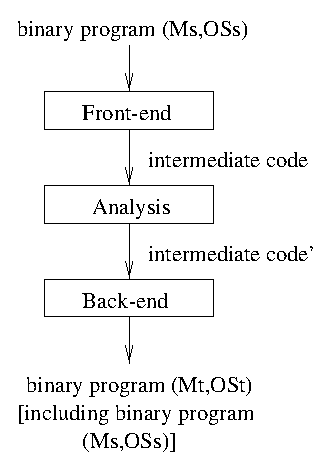
\includegraphics{figures/static.eps}}
\centerfigend{fig-static}{Structure of a static binary translator for
	source machine $M_s$, target machine $M_t$, source operating system
    $OS_s$ and target operating system $OS_t$.}
 
The fallback mechanism used by static binary translators is a runtime
environment that completely supports the source platform, and
hence includes an interpreter for source machine instructions, and support
for translation and mapping of operating system calls into the new
platform.  The development of a runtime environment is a significant
overhead; especially the mapping of operating system calls.  There is
little performance data reported in the literature regarding the amount of
time spent by binary translated applications in the interpreter mode.
Code ported from a proprietary CISC to RISC machine at Tandem, where the
operating system was binary translated to the new machine, reports an
average figure of 1\% of the time being spent on interpretation~\cite{Andr92}.
Informal talks with people who have developed such translators state that
the interpretation mode is seldom used if you have sufficient coverage 
of the patterns generated by compilers commonly used in that platform. 
Existing static translators have dealt mainly with procedural code, 
rather than object-oriented code, which poses new limitations to static
translation due to their dynamic nature of code dispatching through 
vtables.  
 
 
\subsection{Dynamic binary translator}
A dynamic binary translator performs the translation of the code while 
the program is being executed by the translator; that is, the input 
binary program is dynamically analyzed and translated into the target 
machine code during runtime.
Dynamic translation techniques overcome some of the shortages of static
translation, for example, determining the targets of indirect jumps.
Dynamic translation is able to support most practical cases of 
self-modifying code; code normally not supported in static translations.
Given that all the processing of a dynamic translator is done ``on the
fly'', the types of optimizations and analyzes have to be carefully
considered and optimized so that the minimum amount of time is spent
during runtime.
 
The structure of a dynamic binary translator is depicted in
Figure~\ref{fig-dynamic}\footnote{
Figure~\ref{fig-dynamic} by the SELF team at Sun Microsystems Labs.}.  
The binary program is fed into the front end which generates an 
intermediate representation for a block of code.  This representation 
is then compiled or emulated by the translator to generate
(unoptimized) machine code for the target machine.  If at any time the
translator determines that a new region of the program needs to be decoded,
the front end is dynamically invoked to parse that region and provide the
intermediate representation.  When generating machine code, counters are
kept on the number of times blocks of code are executed; once a threshold is
reached, machine code is regenerated to produce better machine code---this
process can be repeated several times, hence producing better code on a
demand-driven basis.  It is important to note that the translation is done
in a lazy fashion; that is, code is only translated when its path is reached.
In this way, fragments of the program that are not executed during runtime,
are not translated either.  Self-modifying code is handled by
invalidating the existing intermediate representation and re-parsing
the binary code with the changed bytes.
 
\centerfigbegin
\resizebox{!}{6cm}
{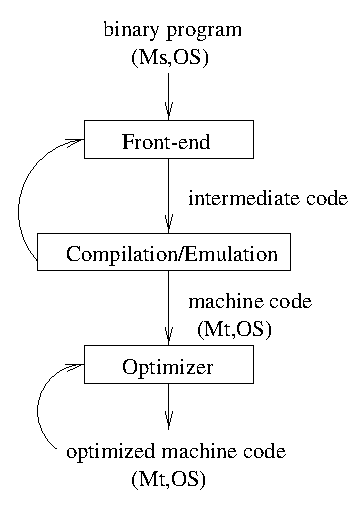
\includegraphics{figures/dynamic.eps}}
\centerfigend{fig-dynamic}{Structure of a dynamic binary translator for
    a source machine Ms, a target machine Mt and a multi-platform
    operating system OS.}
 
Dynamic compilers can perform runtime optimizations of the code based
on the execution profile of the program, hence several optimizations,
such as dynamically-dispatched calls and procedure inlining, can only be
possibly done on a dynamic compiler rather than using static techniques.
The performance penalty of code generated by such a translator is estimated
between 0.9X to 2.4X times that of code generated by a native optimizer
C++ compiler (these figures are based on code generated by the SELF-93 dynamic
compiler~\cite{Holz95}).
 
An interesting point to note is that a dynamic binary translator for
a multi-platform operating system does not require the development of
a runtime environment to support the mapping of old operating system
calls, as all translations are done ``on the fly''.  Using static techniques
in this case will still require a runtime environment to cater for the
interpretation of old machine instructions--dynamic techniques alleviate
the need for this fallback mechanism, but compromise the speed of 
execution of the program at the expense of less analysis and code
quality.
 




	
\chapter{Previous Work}
\label{ch-prevwork}

{\small
\begin{flushright}
Documentation: Cristina [c.1996, 2001]
\end{flushright} 
}

Binary translation is a relatively new field of research, were the
techniques are derived from the compilation, emulation and decompilation areas. 
Nevertheless, the techniques are ad hoc in nature and little has been 
published about them (mainly driven by commercial interests of the parties
involved).  

In this chapter we describe the related work, which we have classified
into two main groups: works related to binary translation and interpreters 
(or emulators), and works related to binary-code manipulation tools that 
may aid in the process.


\section{Binary translators and interpreters} 
Binary translation techniques were developed from emulation
techniques at research labs in the late 1980s.  Projects
like the HP3000 emulation on HP Precision Architecture
computers~\cite{Berg87} and MIMIC, an IBM System/370 simulator on an
IBM RT (RISC) PC~\cite{May87} were the catalist for these techniques.
One of the goals of the HP project was to run existing MPE V binaries
on the new MPE XL operating system.  For this purpose, a compatibility
mode environment was provided, which was composed of two systems:
a HP 3000 emulator and a HP 3000 object code translator.  The emulator
duplicated the behavior of the legacy hardware, and the translator
provided efficient translated code which relied on the emulator
when indirect transfers of control where met.

Tandem developed an object code translator for TNS CISC binaries
to TNS/R (RISC) in order to provide a migration path for existing
vendor and user software~\cite{Andr92}.  This approach allowed
them to market their new RISC machines years earlier than if no
migration path was available.  Part of the rationale for the
project was also the fact that no reprogramming was involved and
that the techniques would provide faster code than emulation
techniques.  Less than 1\% of the time was spent on emulation.

Digital developed two translators, VEST and mx, to provide a migration
path from their OpenVMS VAX and Ultrix MIPS systems to their new
Alpha machine~\cite{Site92,Site93}.  Interestingly enough, they
decided to do careful static translation once instead of on-the-fly
dynamic translation at each execution time for performance issues.
In both their translators, the old and new environments were, by
design, quite similar, plus both provided similar operating system
services.  Some of the goals were to take full advantage of the
performance capabilities of the Alpha and avoiding the problem of
not having all the tools available to port a program to a new architecture
(because they are still not available on the new hardware).
This was seen as an interim solution, while the user's environment was
made available on the new machine and then code could be recompiled/rebuilt.

Up to 1992 all translators were made available by hardware                   
manufacturers to provide a migration path from their legacy
hardware platform (normally a CISC) to their new platform
(normally a RISC).

Back in 1994, AT\&T Bell Laboratories provided services to migrate
software in object code form from one platform to another through
the FlashPort binary translator~\cite{Att94}.
Translations of PDP 11, 680x0 and IBM 360 code was made to
platforms like MIPS, RS/6000, PowerPC and SPARC.  Translation
time was based on the type of application, with some large
applications being translated in 1 month, whereas others in
6 months; which means that manual changes were done to assure
consistency of the translation, plus to provide compatibility
libraries to cater for the differences in operating systems and
services.
The FlashPort technology was initially developed by Bell Laboratories
researchers and was commercialized through the 1991-formed Echo
Logic company.  The first production release of the technology
was provided to Apple Computers in 1993 to translate Macintosh
binaries to the then forthcoming PowerPC-based Macintosh computers.

In an attempt to make Alpha machines more appealing to existing
Unix users, Digital released FreePort Express, a SunOS SPARC
static binary translator to Digital Unix Alpha~\cite{Dec95};
particularly at a time when Sun was migrating customers to
their new Solaris OS and discontinuing support for SunOS.
The tool was advertised as a way of migrating to the Alpha even
when source code and compiler tools from the source machine
were not available; then do a native port at your own leisure.
Since the translated programs and libraries provided support for
Xview, OpenLook, Motif and other X11-based applications, this
migration path was suitable for users who did not want to be
trained in the use of new tools.

To improve Alpha's usability as a desktop alternative to Intel
PCs, Digital developed FX!32, an WindowsNT x86 to WindowsNT Alpha
translator~\cite{Thom96,Hook97}.  Emulation was used as it provided
a quick way to provide support for changes in WindowsNT.  However,
binary translation on the background was also used in order to
save the translations to a file and, over time, incrementally
build the new Alpha binary.  This hybrid translator uses profiling
information in order to optimize the code the next time it
is run.

The TIBBIT project looks at real-time applications that are to be
binary translated between processors of different speeds~\cite{Cogs95,Cogs95b}.
The translated software needs to retain the implicit time-dependency
of the old software in order to function correctly.

\begin{table*}[hbtp]
{\footnotesize
\begin{tabular}{|p{1.5cm}|p{1.3cm}|p{0.7cm}|p{5cm}|p{2cm}|p{2cm}|} \hline
Name & Affiliation & Ref & Purpose & Source Platform & Target Platform \\ \hline
Bergh et al (1987) & HP & \cite{Berg87} &
	Software emulation and object code translation. &
	(HP3000, MPE V) &
	(HP Precision Architecture, MPE XL) \\
Mimic (1987) & IBM & \cite{May87} &
	Software emulator with a 1:4 code expansion factor per 
	old machine instruction. &
	IBM System/370 &
	IBM RT PC \\
Johnson (1990) & Stardent & \cite{John90} &
	Postloading optimizations. &
	RISC &
	RISC \\
Bedichek et al (1990) & U.Wash & \cite{Bedi90} &
	Efficient architecture simulation and debugging. &
	Motorola 88000 &
	Motorola 88000 \\
Accelerator (1992) & Tandem & \cite{Andr92}        &
	Static binary translation for CISC to RISC migration.  
	Uses a fallback interpreter.    &
	TNS CISC        &
	TNS/R   \\
VEST, mx (1993) & Digital & \cite{Site93} &
	Static binary translation from Digital's VAX and MIPS machines
	to the 64-bit Alpha.  Uses a fallback interpreter. &
	(VAX, OpenVMS), (MIPS, Ultrix) &
	(Alpha, OpenVMS), (Alpha, OSF/1) \\
Wabi (1994) & Sun & \cite{Sun94} &
	Pretranslated Windows API to Unix API calls.  Dynamic execution of 
	programs. &
	(x86, Windows 3.x) &
	(SPARC, Solaris) \\
Flashport (1994) & AT\&T & \cite{Att94} &
	Binary translation across a variety of source and target platforms.
	Requires human intervention. & 
	680x0 Mac, IBM System/360, 370, 380 &
	PowerMac, IBM RS/6000, SPARC, HP, MIPS, Pentium \\
Shade (1994) & Sun & \cite{Cmel94} &
	Efficient instruction-set simulation and trace generation
	capability.  Dynamic compilation of code. &
	SPARC V8, V9 &
	SPARC V9, V8 \\
MAE (1994) & Apple & \cite{Apple94} &
	Macintosh environment in an XWindow, Unix RISC-based workstation. &
	680x0 &
	RISC-based Unix \\
Wahbe et al (1994) & CMU & \cite{Wahb94} &
	Adaptable binaries.  Binary transformations.&
	(MIPS, Ultrix4.2) &
	(MIPS, Ultrix4.2) \\
Chia (1995) & Purdue & \cite{Chia95} &
	Software emulation within the same platform, with a 1:100 code
	expansion factor per old machine instruction. &
	(SPARC, Solaris) &
	(SPARC, Solaris) \\
TIBBIT (1995) & CMU, UO & \cite{Cogs95,Cogs95b} &
	Binary translation of time-sensitive applications.&
	Motorola 68000 &
	(IBM RS/6000, AIX 3.2) \\
Then (1995) & Purdue & \cite{Then95} &
	Optimization of code within the same platform.&
	(SPARC, Solaris) &
	(SPARC, Solaris) \\
Freeport Express (1995) & Digital & \cite{Dec95} &
	Static binary translation and fallback interpreter.  Translates
	user mode programs. 32-bit to 64-bit translation. &
	(SPARC, SunOS4.1.x) &
	(Alpha, OSF/1) \\
FX!32 (1996) & Digital & \cite{Thom96,Hook97} &
	Hybrid emulator/binary translator of popular x86 32-bit applications 
	to Alpha.   &
	(x86, WindowsNT) &
	(Alpha, WindowsNT) \\
\hline
\end{tabular}
\caption{\label{tab-bintrans} {Summary of Binary Translators and
	Interpreters in Cronological Order.}}}
\end{table*}

We summarize the features of a variety of binary translators and
interpreters in Table~\ref{tab-bintrans}.  The column {\em Purpose\/} 
describes the general use of the tool, columns {\em Source Platform\/}
and {\em Target Platform\/} describe the nature of the translation supported
by the tool (i.e. multi-platform or within the one platform), 
column {\em Name\/} refers to the name of the software; if unnamed, then
it refers to the people that worked on it, and column {\it Affiliation}
refers to the affiliation of the authors of the software at the time
of development. 


\subsection{List of recent translators}
There has been a lot of work in the last few years (1998-2000) 
on dynamic techniques for doing binary manipulation of one sort of 
another.  The following is a list of projects and literature available: 

\begin{itemize}
\item HP Aries~\cite{Zhen00}: 
Aries is a hybrid interpreter/dynamic translator which
allows PA/RISC HP-UX binaries to run in an IA-64 HP-UX
environment transparently, without user intervention.

\item HP Labs Dynamo~\cite{Bala00}: 
Dynamo is a dynamic reoptimizer of PA-RISC binaries which
produces PA-RISC code.  It works well for some programs 
and not for others. 

\item IBM TJ Watson Research Center's DAISY~\cite{Ebci96} and 
BOA~\cite{Gsch00}: 
The DAISY and BOA projects have looked at dynamic binary translation 
from conventional architectures such as the PowerPC to VLIW or other
novel architectures.  Their work addresses precise exceptions, 
self-modifying code, and reordering of memory references; all of 
these from an architectural point of view. 

\item Transmeta's Crusoe~\cite{Gepp00}: 
The Crusoe chip is a VLIW chip which includes code morphing to 
dynamically binary translate from x86 to the VLIW instruction set. 
Some x86 instructions are supported by the hardware itself. 

\item Compaq's Wiggins/Redstone~\cite{Reev00}: 
Wiggins/Redstone was a dynamic reoptimizer of Alpha binary code. 
It was built based on Digital's DCPI infrastructure.  

\end{itemize}



\section{Binary-code manipulation tools}

\begin{table*}[hbtp]
{\small
\begin{tabular}{|p{2.0cm}|p{0.7cm}|p{7.8cm}|p{3.0cm}|} \hline
Name & Ref & Purpose & Platform \\ \hline
Silberman et al (1993) & \cite{Silb93} &
	Framework for supporting heterogeneous instruction set architectures. &
	CISC, RISC, VLIW \\
QPT (1994) & \cite{Laru94} &
	Rewrite executable files to measure program behavior. &
	MIPS, SPARC \\
Shade (1994) & \cite{Cmel94} &
	Execution profiling of application binaries. &
	SPARC V8, V9 \\
ATOM (1994) & \cite{Dec94,Eust95} &
	Sytem for building customized program analysis tools. &
	(DecStation, Ultrix), (Alpha, OSF/1) \\
NJMC (1994) & \cite{Rams95,Rams94,Rams97} & 
	Machine-independent encoding and decoding of machine instructions
	via the SLED language. &
	MIPS, SPARC, x86, PowerPC, Alpha \\
EEL (1995) & \cite{Laru95} &
	Library for editing binaries. &
	MIPS, SPARC \\
\hline
\end{tabular}
\caption{\label{tab-bintools} {Summary of Binary-code Manipulation  
	Tools in Cronological Order.}}
}
\end{table*}

Table~\ref{tab-bintools} summarizes the available tools for handling
machine binary code.  The column \emph{Name} lists the name of the
tool (or its author if no name was given to the tool), column 
\emph{Ref} lists the references in the literature to this tool,
column \emph{Purpose} describes the purpose of the tool, and column 
\emph{Platform} lists the platform(s) supported by these tools. 

ATOM is a tool-building system that provides a flexible and efficient
interface for the instrumentation of code and has been used for the
construction of an instruction profiler, cache simulator and compiler
auditing tool~\cite{Eust95}.  The user needs to write an instrumentation
file in terms of ATOM's abstractions (procedures and basic blocks),
and an analysis file (using a high-level language such as C) with the 
routines that are to be included for instrumentation purposes.  
The performance of the generated tools compare favourably with 
hand-crafted implementations of same the tools. 

Shade is an instruction-set simulator which optionally allows users to 
profile code that traces the execution of an application at runtime.  
Trace information on instruction addresses, instruction text, decoded
opcode values, and more can be collected by Shade~\cite{Cmel94}.
This tool works only on SPARC machines.

Both NJMC (New Jersey Machine-Code) toolkit~\cite{Rams95,Rams97} and EEL
(Executable Editing Library)~\cite{Laru95} provide support for
manipulating machine instructions.  The NJMC toolkit supports the 
encoding and decoding of machine instructions for a variety of 
RISC and CISC machines, by means of SLED specifications.  
The SLED language allows for the description of the syntax of machine 
instructions in a specification that resembles instruction descriptions 
found in architecture manuals.
The toolkit has successfully been used in a retargetable 
linker~\cite{Fern95} and a retargetable debugger~\cite{Rams92}.  
The EEL library was built based on the NJMC machine specifications, 
and introduced control flow support based on techniques developed in 
the QPT~\cite{Laru94} profiler.  EEL also introduced limited
support for describing the semantics of machine instructions.
The tool is not fully portable to non RISC environments.




	
\chapter{The UQBT Framework}
\label{ch-uqbt-framework}

{\small
\begin{flushright}
Design: Cristina, Norman; Documentation: Cristina [c.98, May 00, Nov 01]
\end{flushright} 
}

The University of Queensland Binary Translator (UQBT) 
framework, is designed to support experimentation in static
binary translation.
UQBT strives to adapt easily to changes in both source and
target machines at low cost, including translations to
register-based and stack-based machines.
Support for multiple architectures is provided by means
of specification of properties of machines, as well as 
conventions used by operating systems.  
This chapter describes the overall architectural organization
of \uqbt\ (Section~\ref{sec-arch}) and its components from the point of view 
of instruction translation (Section~\ref{sec-framework}).  Note that
these two sections are necessarily overlapping; the former
section reflects more of the design and the latter section
reflects more of the implementation of the system.  
The chapter concludes with a small section on the state of the
UQBT framework at the end of 2001. 


\section{The Proposed 1997 Architecture of a Retargetable Binary Translator}
\label{sec-arch}

Like a compiler and a decompiler, a binary translator can logically
be divided into three phases: front end, analysis and transformation,
and back end.  For a given source machine M$_s$ and destination machine M$_d$,
the front end decodes machine M$_s$'s binary file and stores the 
information in a machine-independent intermediate form based on RTLs.
The analysis phase maps machine M$_s$'s locations onto machine M$_d$'s 
locations and transforms the RTLs so that they can be readily translated into 
native code for machine M$_d$.  The back end translates the intermediate 
form and writes a binary file for machine M$_d$.  It may also optimize 
instructions.

From a retargetability point of view, it is more helpful to think of 
a functional division into components instead of a sequential division 
into phases.  Such components may be used in more than one phase.
Some components will be machine-independent; others may be generated 
from machine descriptions.  In Figure~\ref{fig-architecture}, we identify 
components by putting them in boxes.

% original file created in Visio, printed to a file using Adobe's Default
% Postscript Printer driver (option EPS), and crop with ghostview (gsview 
% on the PC version 2.5) using File->PStoEPS option.
\centerfigbegin
\resizebox{!}{10cm}
{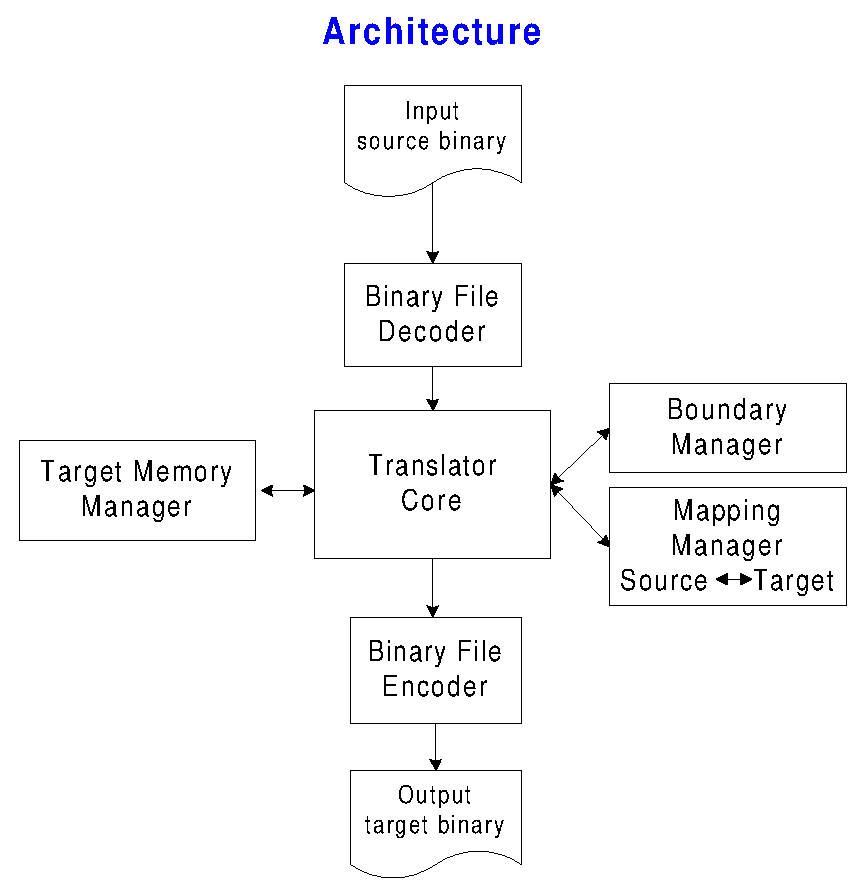
\includegraphics{figures/uqbt_architecture.eps}}
\centerfigend{fig-architecture}{Architecture for a Retargetable Binary
	Translator.  Components are Represented in Boxes.}

Implementation of components draws on techniques developed for
dcc, an 80286 decompiler~\cite{Cifu95}, for specifying
representations of machine instructions~\cite{Rams97},
and for the U.S. National Compiler Infrastructure project.


\subsection{Components}

M$_s$ \emph{binary file reader} exports an abstraction
representing the contents of the executable binary on the original
machine.  This module promotes retargetability by hiding
information about the source machine that one might otherwise be
tempted to exploit.  The capabilities exported include:
%\enumerateAlpha
\begin{enumerate}
\item The initial state of the M$_s$ processor that would apply when about
     to run this binary on a native M$_s$ processor, including at minimum
     the value of the program counter,
\item A list of potential entry points for procedures, possibly empty
     (N.B. the initial program counter is always available as an entry
     point), 
\item The ability to fetch the program's code and data, by the address
     those contents would occupy in a running M$_s$ executable, and 
\item The ability to identify calls to dynamically linked procedures, and
     to provide access to the code and data associated with those
     procedures.
\end{enumerate}
%\enumerateNumber
This module may therefore include much of the functionality of a dynamic
linker/loader.

One of the crucial decisions made by a translator is which locations
on machine M$_d$ hold what data from machine M$_s$.  We will encapsulate these
decisions in a \emph{mapping manager}, which will map locations in code
space, locations in data space, and locations referring to registers
or other processor state.  Most mappings will be determined
automatically at translation time, but some mappings may be specified
by hand for each pair of platforms, e.g., what registers of machine M$_d$
should be used to represent the contents of registers of machine M$_s$.

The mapping manager will rely on the M$_d$ \emph{memory manager} to allocate 
locations in the destination machine's storage space, e.g., to store 
translated code.

Because it is impossible to identify and translate all code, a running
image on machine M$_d$ will in general have a mix of translated and
untranslated code.  The \emph{boundary manager} will track the boundary
between translated and untranslated code and handle flow of control
across the boundary.  For example, a branch from translated to
untranslated code might go to an interpreter or to a dynamic
translator.  If the untranslated code is subsequently translated, the
boundary moves, and the boundary manager might backpatch the branch.

The \emph{core translator} will translate groups of machine instructions.
A group may be as small as a basic block or as large as an entire 
program, and different translation strategies (e.g., full static, 
partial static, dynamic) may use different group sizes.

The core translator coordinates the action of all the other
components and performs the main translation analyses.  It will 
translate a group of M$_s$ instructions as follows:
%\enumerateAlpha
\begin{enumerate}
\item Ask the memory manager for a location in M$_d$ to hold the translated
     code, and inform the mapping manager of the new mapping, 
\item Translate M$_s$ instructions to M$_d$ instructions
	  \begin{itemize}
      \item using information from the mapping manager to translate
         access to machine M$_s$'s data, 
      \item using information from the boundary manager to translate flow
	  \end{itemize}
	 of control outside the current group, and
\item Inform the boundary manager of the translation of the current group.
     The boundary manager may choose to backpatch branches into the
     current group.
\end{enumerate}
%\enumerateNumber
Depending on the granularity and timing of translation, these steps may
be repeated on other units until some termination condition is met.
If the granularity of translation is sufficiently large, the second step
may involve translating into an intermediate form and doing some global
analysis and optimization.

Finally, the M$_d$ \emph{binary file writer} will export an abstraction
representing the ability to create an executable binary on machine M$_d$.
It will export the abilities to:
%\enumerateAlpha
\begin{enumerate}
\item Specify the contents of the M$_d$ address space at the start of
     execution,
\item Establish the state of the M$_d$ processor at the start of execution,
\item Write an executable binary file in the M$_d$ native format, and
\item Possible support for dynamic linking, e.g. of translated or native
     libraries.
\end{enumerate}
%\enumerateNumber
In a dynamic translator, this component would simply write into a
running process image (and possible flush the I-cache).


\subsection{Core Translation based on RTLs}

The translation itself will be performed using register transfer lists
(RTLs).  An RTL is a collection of simultaneous effects.  Each effect
has the form `location := expression', and the expression is always
evaluated without side effects, so all state change is explicit.  
RTL expressions are represented as trees, the leaves of which refer to
constants or to the values contained in locations.  Note that although
the tree leaves refer to locations, the values themselves are not
necessarily calculated, only the location is referenced.
The internal nodes of the trees are `RTL operators'.  
For illustrative purposes, the following is an ASCII representation of an 
RTL representing the effect of the SPARC \texttt{andcc} instruction:
\begin{smallverbatim}
 $r[rd] <--      and (*$r[rs1], if i = 0 then *$r[rs2] else simm13! fi);
 icc.N  <-- bit (and (*$r[rs1], if i = 0 then *$r[rs2] else simm13! fi) < 0);
 icc.Z  <-- bit (and (*$r[rs1], if i = 0 then *$r[rs2] else simm13! fi) = 0);
 icc.V  <-- 0;
 icc.C  <-- 0
\end{smallverbatim}
This RTL does a bitwise AND of the contents of register rs1, either
with the contents of register rs2 or with a signed immediate value (simm13).
This result is stored in register rd, and it is also used to set two
of the four condition codes.  The other two condition codes are set to 
zero by the instruction.

RTLs are obviously complex and detailed.  Machine descriptions
themselves will be written at a higher level of abstraction and
compiled into RTLs.  Run-time representations of RTLs will be
`collapsed' either by analyzing these higher-level representations or
by using the `superoperator' technique~\cite{Proe95}.  
For example, we might define a superoperator LOGICAL such that LOGICAL(X)
stood for
\begin{smallverbatim}
 $r[rd] <--      X;
 icc.N  <-- bit ((X) < 0);
 icc.Z  <-- bit ((X) = 0);
 icc.V  <-- 0;
 icc.C  <-- 0
\end{smallverbatim}
Such a superoperator could be derived from the SPARC description. 

An `RTL language' is defined by a collection of locations and
operators.  For binary translation, a suitable RTL language can be
defined by taking the union of locations on machines M$_s$ and M$_d$ and the
union of the operators used in the descriptions of machine M$_s$ and M$_d$.
The `machine X invariant' defines a sub-language of RTLs called the
X-RTLs; an RTL is an X-RTL if and only if it can be represented as a
single instruction on machine X.

% original figure in Visio, exported as eps (without including TIFF
% preview or background rectangle).
\centerfigbegin
\resizebox{!}{12cm}
{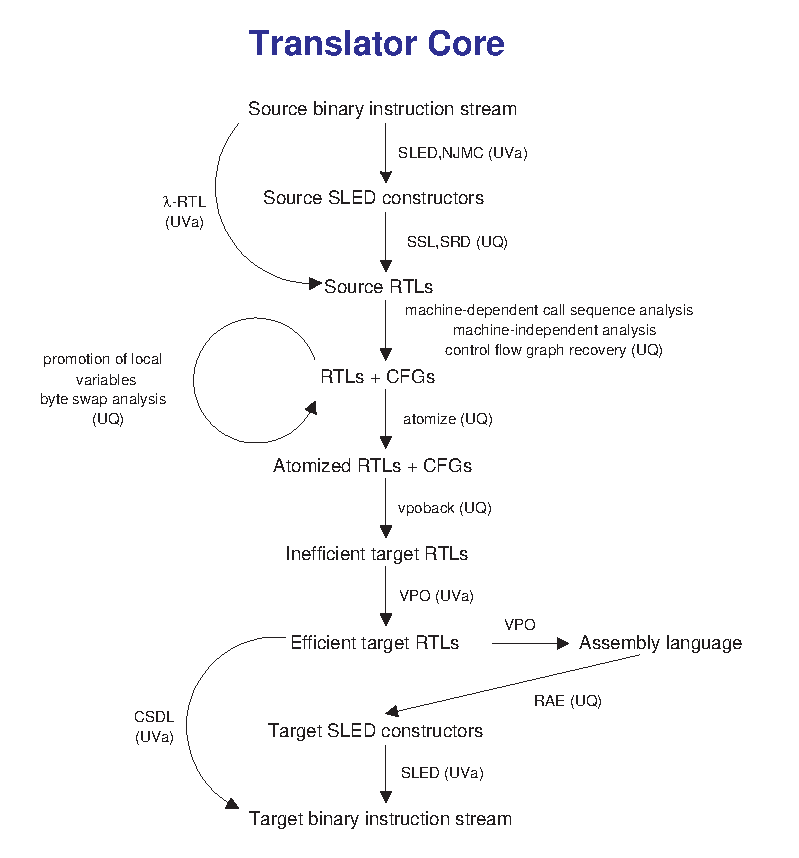
\includegraphics{figures/uqbt_dataflow.eps}}
\centerfigend{fig-dataflow}{Flow of Data through the System}

As shown in Figure~\ref{fig-dataflow}, the main steps in the translation are:
\begin{enumerate}
\item Decode the binary stream into M$_s$-RTLs.  This step will be
     automated by specifying syntax and semantics of M$_s$ instructions.

\item Build a control flow graph (CFG) for each procedure.  Analysis
     will be needed to find code associated with a procedure.

\item With the help of the mapping manager, map the machine M$_s$ locations
     in the RTLs to machine M$_d$ locations or to temporaries.

\item `Atomize' the RTLs to expose all RTL operators at top level, and
     find suitable replacements for machine M$_s$ operators that are not
     available on machine M$_d$.  For example, big-endian memory access
     might be replaced with explicit byte swapping.

\item Reassemble the RTLs to satisfy the machine M$_d$ invariant, making
	them M$_d$-RTLs (i.e. M$_d$-RTLs have a 1:1 mapping with M$_d$ 
	assembly instructions).

\item Optimize the M$_d$-RTLs using VPO~\cite{Beni88} or any other RTL 
	optimizer.

\item Encode the M$_d$-RTLs into binary code for machine M$_d$.  Also automated.
\end{enumerate}

The most challenging steps are steps (4) and (5).  In the initial
stages, these will be implemented by hand; we hope to develop automated
techniques afterwards.  The other steps can be automated based on
machine descriptions or a mapping specification.

Future analyses, intended to improve translated code, might be
implemented after steps (2), (3), or (4).  Such analyses might make it
possible to avoid byte swapping, to use machine M$_d$ calling conventions,
to put machine M$_s$ stack variables in machine M$_d$ registers, etc.
Analyses may vary depending on the granularity of translation.


\section{The 1999 UQBT Framework}
\label{sec-framework}

In order to support resourceability and retargetability, 
machine descriptions of machine properties are needed, 
as well as descriptions of conventions and formats used by 
the operating system.  We have identified 6 different specification 
languages and/or APIs to support the UQBT framework, 4 of these are 
currently in use in our framework. 

The framework described in this section dates from 1998, 
Section~\ref{sec-2001framework} describes the 2001 framework. 
References in this section are to papers and chapters within 
this book that explain in more detail a particular concept. 


\subsubsection*{Machine specifications and APIs} 
Properties of a machine are represented in terms of the machine 
instructions (i.e. the mnemonics), the semantics of such instructions, 
the identification of the instructions that transfer flow of control, 
and, if needed, delayed transfers of control information.  
These 4 types of information are represented by the following 
languages: 

  \begin{itemize}
  \item SLED (Specification Language for Encoding and Decoding), 
	which supports descriptions of the syntax of machine 
	instructions~\cite{Rams97}.  [Chapter~\ref{ch-decoding}];

  \item SSL (Semantic Specification Language), which supports 
	descriptions of the semantics of machine 
	instructions~\cite{Cifu98c}.  [Chapter~\ref{ch-ssl}]; 

  \item CTL (Control Transfer Language), which supports the 
	identification of instructions that perform control 
	transfers of control (conditional jumps, jumps, calls or 
	returns). This language was implemented as a loose API in the
	end, as we decided not to specify other transfer of control 
	information in the end.  

  \item DCTL (Delayed Control Transfer Language), which supports 
	the description of simple transformations needed in 
	order to remove dependencies on delayed instructions (in 
	machines that support such concept).  

    Support for DCTL is not in place at present.  Initially, we used 
    a program-transformation and partial-evaluation technique to derive 
    the transformations on instructions that support delayed transfers of 
    control~\cite{Cifu98i}.  [Chapter~\ref{ch-delay}].
    The code is voluminous and we believe that code to support such 
    transformations could be automated from a short specification 
    of the required transformations.  This step would clearly increase 
    the resourceability of the framework.  However, we note that not 
    too many machines currently support the delayed-slot transfer of 
    control, only SPARC, PA-RISC and MIPS do at present time.

  \end{itemize}


\subsubsection*{OS specifications/APIs} 
Conventions and formats used by a multiplatform operating system come 
in the form of calling conventions, including where parameters are passed 
(i.e. stack or registers), and the format of the binary-file that the 
OS supports.  
These 2 pieces of information are represented by the following 
languages/APIs: 

  \begin{itemize}
  \item PAL (Procedural Abstraction Language), which supports 
	the description of calling conventions, parameter passing conventions, 
	and local variables conventions~\cite{Cifu99g}. [Chapter~\ref{ch-call}];  
	and 

  \item BFF (Binary File Format), which supports the description 
	of the internal format of a binary-file, such as the 
	Elf format on Solaris and Linux systems~\cite{Cifu97f}. 
	[Chapter~\ref{ch-bff}].  
  \end{itemize} 

We currently support the PAL language and have worked on 
an initial prototype of the BFF language, which is incomplete 
at present time but proves the feasibility of specifying 
binary-file formats and automatically generating code to 
support the decoding of such files.  In our experience, it 
was easier to have a set API for dealing with differences in 
binary-file formats than to specify the existing ones.   

\psfigbegin{figures/uqbtImplementation.eps}{10cm}
\psfigend{fig-uqbt}{Framework for a Resourceable Binary Translator.}

Figure~\ref{fig-uqbt} illustrates the components of the 
translation process in the form of boxes.  Specifications for different
machines are illustrated with the document shape.
Greyed-out shapes mean that they are not currently supported 
by UQBT and therefore an implementation for a particular format 
or analysis has been done instead.  Arrows represent conceptual 
flow of control in the translation process.  


\subsection{The Decoding Phase}
The binary-file decoder, instruction decoder 
and semantic mapper translate raw machine instructions into  
M$_s$-RTLs for a given source machine M$_s$.  
As previously mentioned, we consider M$_s$-RTLs machine dependent, as
they represent how the source machine performs a given instruction, 
including delayed-slot semantics for example.  

In static translators, the amount of decoding from this phase 
is limited by indirect transfers of control (i.e. statically,  
it is not always possible to determine the target of an 
indexed jump or an indirect call).  
UQBT includes a slicing-based technique to determine the target
address(es) of indirect transfers of control~\cite{Cifu99c}. 
This technique allows us to decode a larger percentage of the
code than otherwise possible, and is reusable across different 
platforms.  


\subsection{The Analysis Phase} 
The translation of M$_S$-RTLs up to \hrtl\ is 
the most challenging stage of the translator.  As seen in 
Figure~\ref{fig-uqbt}, this translation requires information 
about control transfer instructions, delayed control transfers 
(if any), parameter and calling conventions, and locals and 
stack frame conventions.  
CTL specifications allow us to translate low-level register 
transfers into higher level instructions such as calls and 
returns.  
For example, a CTL specification for SPARC states that a 
jump and link instruction with destination register \texttt{\%o7} 
is a call instruction.  This semantics is not necessarily 
obvious from the SSL description of a jump and link instruction. 
Further, the same instruction using destination register 
\texttt{\%g0} is equivalent to an unconditional jump; this 
too is specified in CTL.  

DCTL specifications will allow us to remove delayed-slot 
instructions in a more machine-independent way.  
At present, as previously mentioned, we implement a program
transformation and partial evaluation technique. 

PAL specifications allow us to recover some of the high-level nature 
of the code, by recovering actual parameters and return 
values for functions, and removing the M$_S$-RTL-specific 
instructions that form part of procedure prologues and 
epilogues, as these are represented in different ways in 
different machines.  The analysis is based on live and 
used parameter and return locations; such locations being
specified in a PAL specification, as well as abstraction to 
an abstract frame pointer (\texttt{\%afp}).  
For example, a PAL specification for the Pentium would specify
that parameters can be passed on the stack and that return 
values go into certain registers (\texttt{\%eax} and top of 
the floating point stack). 
A more detailed description of the analysis is available 
in~\cite{Cifu99g} and Chapter~\ref{ch-call}. 
 
\centerfigbegin
\begin{fnverbatim}
r[tmp] = %sp
r[tmp2] := -120
%pwp = %cwp
%cwp = %cwp + 64
%cwp = (%cwp-1) % NWINDOWS
%sp = r[tmp] + r[tmp2]
r[9] = 69 << 10            v1 = 70656
r[8] = r[9] | 720          v0 = v1 | 720
r[15] = %pc
%pc = %npc
%npc = 0x21780             Call printf (v0, v1)
r[9] = r[30] + -20         v1 = %afp + 100
r[10] = 69 << 10           v2 = 70656
r[8] = r[10] | 736         v0 = v2 | 736
r[15] = %pc
%pc = %npc
%npc = 0x2178c             Call scanf (v0, v1, v2)
r[8] := m[r[30] - 20]      v0 = m[%afp + 100]
r[15] = %pc
%pc = %npc
%npc = 0x10a9c             v0 = Call fib (v0)
m[r[30] - 24] = r[8]       m[%afp + 96] = v0
\end{fnverbatim}
\centerfigend{fig-palEg}{Example of the result of the use of PAL
        specifications to translate SPARC-RTL code (left-hand side)
        to \hrtl\ (right-hand side) in a fibonacci program.}

Figure~\ref{fig-palEg} illustrates 
a snippet of SPARC-RTLs for the \texttt{main} of a fibonacci 
program, and the resultant \hrtl\ code.  As can be seen, 
the RTLs for the procedure prologue were removed (and relevant information
used in the translation), the actual parameters to library functions 
\texttt{printf} and \texttt{scanf} are listed, actual parameters 
were moved to variable locations, local variables are in terms of 
an abstract frame pointer called \texttt{\%afp}, and the return 
value for the call to \texttt{fib} has been determined.   
The example also shows that the call to \texttt{fib} has the
right number of parameters (i.e. one), and that the calls to
the variable argument routines \texttt{printf} and \texttt{scanf} 
each take one extra parameter than expected.  These parameters were passed 
as they were live and were valid parameter locations at the 
call site.  However, when the code is executed, these parameters
will not be used as the library routines would not be expecting
these parameters for processing (i.e. the format string 
in both these routines specifies the number of parameters
required to be processed), therefore producing the right
result at runtime.  

Lifting the level of representation of the code to \hrtl\ 
allows for experimentation with different types  
of binary translation-specific optimizations, such as removing 
some of the byte swaps at loads and stores when machines have  
different endianness, or promoting local variables to registers. 
This is future work. 


\subsection{The Encoding Phase} 
\label{sec-encoding}

\centerfigbegin
\begin{fnverbatim}
void main() {
int v0;
int v1;
int v2;
char _locals[120];

        v1=70656;
        v0=(v1)|(720);
        printf(v0,v1);
        v1=(_locals)+(100);
        v2=70656;
        v0=(v2)|(736);
        scanf(v0,v1,v2);
        v0=*((int*)((_locals)+(100)));
        v0=fib(v0);
        *((int*)((_locals)+(96)))=v0;
\end{fnverbatim}
\centerfigend{fig-cEg}{Example generated low-level C code for the partial
        fibonacci example of Figure~\ref{fig-palEg}.}

The last step in this phase is the translation down to the 
target machine's intermediate representation; M$_T$-RTL in 
the case of register-based machines or \bcode\ in the case 
of stack-based machines.  
The translated code will always require an optimizer to improve 
its quality, therefore, the encoder phase would be equivalent 
to that of an optimizing compiler.  Because we interface 
to existing C optimizing compilers, we generate very low-level 
C code from this step.  Figure~\ref{fig-cEg} shows the 
generated low-level C code for the example in Figure~\ref{fig-palEg}. 
As can be seen, data addresses are not modified, therefore  
a call to \texttt{printf} or \texttt{scanf} takes the same 
memory address as that in the source binary.  

We have successfully interfaced to VPO~\cite{Beni88}, whose register 
transfer list interface is similar to our RTLs, and hence it is simple  
to translate to.  The new VPO interface is part of the Zephyr 
project~\cite{Vpo98}.  
Generating (low level) C allows us to experiment with different 
optimizers, and also is the interface to the stack based backends. 
For generation of code to the Java Virtual Machine (JVM), we 
have written a backend and a bytecode description that 
integrates with gcc. 

\centerfigbegin
\begin{fnverbatim}
                   ... (setup code)
v2=134517960;      ldc 124517960   ; put string in local 10
printf(v2);        istore 10
r24=(_afp)+(4);    aload_0         ; call _printf
v2=r24;            iload 10
v1=134517975;      invokevirtual Fibo/_printf (I) I
scanf(v1,v2);      istore 10
                   ldc 16          ; put afp+4 in local 12
                   lstore 9
                   iload 14
                   iload 9
                   iadd
                   istore 12
                   ldc 134517975   ; put string in local 10
                   istore 10
                   iload 12        ; put afp+4 in local 11
                   istore 11
                   aload_0         ; call _scanf
                   iload 10
                   iload 11
                   invokevirtual Fibo/_scanf(II)I
                   istore 10
\end{fnverbatim}
\centerfigend{fig-bcodeEg}{Example of generated bytecode after gcc
        optimizations (right-hand side) for low-level C code
        generated from Pentium fibonacci binary (left-hand side).}

The generation of bytecode via gcc provides us with all the
classical optimizations that are too computationally expensive to be
performed by a just-in-time compiler.  
We wrote a bytecode specification file for gcc which treats registers 
as locals and describes peephole optimizations.  
For each \hrtl\ instruction, $n$ bytecode instructions are 
generated, where $n$ is normally less than 5.  The generated
bytecode is similar to that generated by a Java compiler, 
given the high level of abstraction of the \hrtl\ code.  
Current work under development improves on the generated bytecode 
by using an intermediate language called \bcode, which allows 
for stack-based optimizations to be performed, therefore minimizing the 
amount of loads and stores from memory and using the stack 
for temporary values more. 
Figure~\ref{fig-bcodeEg} shows sample bytecode generated from our 
gcc bytecode backend.  Library calls are to wrapping routines 
which invoke the native Java library subsystems.  For variable
argument routines, we have $n$ different wrappers, where $n$ is
the number of parameters and typically $n$ is less than 10. 

For each translation, the generated code and data are 
placed into a variety of C and assembly files which can be 
compiled with gcc and gas on the target machine.  
For each function, a low-level C file is generated. 
For each data section, an assembly file is generated with the  
relevant bytes. 
A makefile is provided to pack the file into an appropriate 
binary for the target machine.

Static translators require the use of an interpreter/emulator to handle 
untranslated code that is discovered at run time.  
The interpreter uses the M$_S$-to-M$_T$ mapping to determine when 
it can return to translated code, and therefore this mapping is stored 
in the target binary.
Because the interpreter will use the original source text section, 
this section is also copied to the target binary.
The interpreter itself is designed to be linked dynamically.
We are currently building a resourceable interpreter/emulator which uses 
the same SLED and SSL specifications provided by the UQBT framework.
The interpreter simulates M$_s$-RTLs and uses PAL specifications 
to determine how to pass parameters to library routines.  
This work is not completed at present time and is under development.

Because of potential aliasing problems, not all of which can be solved by
static analysis, the data sections (generally .rodata and .data in 
Elf binary files) are copied ``as is'' to the target binary. 
They are made to retain the same Virtual Memory Address in the 
target binary as in the source binary. A link map file generated by 
the translator is used to achieve this. The target program calculates 
addresses exactly as the original source program did, and so the data 
is referenced correctly (although it may need to be referenced 
using different endianness). 
Because of differences in size of pages in various architectures 
(e.g. 4Kb on Pentium, verses typically 8Kb on SPARC), this mapping 
cannot always be achieved entirely by manipulation of addresses in the 
target binary file. A very small piece of code sometimes has to perform block 
moves (before the normal startup code) to achieve the correct addresses.

Translators to bytecode require extra environment support
to compliment the strengths of the JVM.  The lack of a generic memory
model on the JVM forces us to emulate the data and stack of a translated
program.  Library functions from the source architecture must also be
supplied to the translated program.  This is facilitated by a superclass
from which each translated program is inherited.  The superclass provides
simulated memory access in preloaded byte arrays and wrapper routines to 
library functions which invoke the native Java subsystems.


\section{The 2001 UQBT Framework}
\label{sec-2001framework}

\psfigbegin{figures/uqbtOverall2001.eps}{10cm}
\psfigend{fig-uqbt2001}{The 2001 UQBT Framework}

The final UQBT 2001 framework provides for several backends that 
were written for experimentation with different ways of generating 
machine code, by integrating at different levels of abstraction. 
Figure~\ref{fig-uqbt2001} shows this framework, we briefly describe
its components next.  In the below description, we divide the framework 
into two sections, the front end and the back end.  The former transforms
binary code to the \hrtl\ representation, the latter transforms down 
from \hrtl\ into another binary representation.

\begin{description}
\item Front end: 
We have one resourceable front end which takes 3 machine and OS 
descriptions and 2 APIs, along with any extra machine-dependent 
code to abstract M$_s$-RTLs into \hrtl\ code.  The parts of the 
front end are: 

\begin{itemize}
\item Binary-file decoder: supports the decoding of the source 
	binary file into an internal UQBT representation that supports 
	the binary-file format API.  The API assumes we can obtain the 
	code (text) and data sections of the file, that there is at 
	least one entry point, and that there may be a symbol table.  

\item Instruction decoder: supports the disassembly of the instruction 
	stream (the text/code section(s)) via the SLED specification for
	the instruction set for the source machine being used.   

\item Semantic mapper: supports the conversion of assembly instructions 
	into RTL instructions, by implementing support for the SSL language, 
	which describes the semantics of assembly instructions. 

\item M$_s$-RTL to \hrtl\ translator: this is the key module in the
	framework that allows us to obtain machine independence in the 
	representation of the code of the program.  This module transforms 
	RTL instructions into \hrtl\ instructions, by supporting an 
	informal control transfer API, performing analyses on procedural  
	information (such as parameters, locals and return locations), 
	and adding any extra hand-written code to support peculiarities 
	of the source instruction set; such as delayed branches on SPARC 
	or floating point stack-based instructions on x86.    
\end{itemize}

The net result of the front end phase is to transform the source 
binary's code into a \hrtl\ representation which is machine independent. 
Transformations on this representation are feasible in order to, 
for example, reduce the number of byte swaps needed when translating 
to different endianness machines.  Transformations of this kind are 
considered binary translation-specific optimizations, as a traditional 
compiler optimizer would not have to deal with them at all.  

\item Back end: 
We have experimented with four different types of back ends.  These 
back ends have commonalities which could be extracted into a common 
back end that supports generation of code at different levels of 
abstraction (such as RTL, assembly or object code).  The back ends are:  

\begin{itemize}
\item C back end: the C backend was the original back end we wrote 
	for the UQBT framework that supported several target platforms 
	(we had earlier experimented with an RTL optimizer).  
	In essence, the C compiler was used as a macro assembler.  
	We translated \hrtl\ code into low-level C code; 
	i.e. code that makes use of goto's and performs a lot of casting 
	of types of expressions.  The generated low-level C code would then 
	be compiled and optimized by the C compiler (we normally compiled 
	using GNU's gcc as well as Sun's cc compilers) and then linked 
	against the original data sections of the source program.  The data 
	sections were always forced to be located at the same memory address 
	space as in the original source program.  

\item JVML back end: the Java bytecode (Java virtual machine language (JVML)) 
	back end was written as an experiment in translating machine code to 
	Java bytecodes.  We translated \hrtl\ code into Java bytecode assembly 
	code, which would be assembled by the Jasmin assembler in order to 
	generate a Java binary (.class file).  Some runtime support was needed 
	as the JVM model is different to that of traditional machines; there 
	was support for dealing with memory, allocating and deallocating memory, 
	as well as support for 32-bit integrals (all integers in the JVM model 
	use 31 bits and are meant to be signed).

\item RTL back end: the RTL back end was an experiment at having more 
	control over the optimizations that were applied to the generated 
	code, as by generating RTL instructions for the target machine, 
	we could then tell an RTL-optimizer to only use certain optimizations 
	and to not move around code in certain sections.   We used the 
	VPO~\cite{Beni88} system for this purpose.  VPO is a retargetable 
	optimizer that now provides an RTL interface to it.  VPO makes use 
	of specifications to describe the syntax of the target instructions, 
	has a series of optimizations that are machine independent, and 
	requires the user to write machine dependent optimizations to support 
	any new machine.  

\item Object code back end: the object code back end was written as an 
	experiment to interface with an optimizer at the object code level, 
	i.e. without having to generate any particular intermediate 
	representation.  The generated code would not do register allocation 
	of any sort, instead, it would place all locations (variables and 
	registers) onto the local stack of a procedure, and would rely on 
	the optimizer to perform register allocation.  This was an internal 
	Sun experiment that made use of a proprietary optimizer, as such, 
	the code is released in the event that it is useful to others, but
	the code for the optimizer is not made available (you can potentially
	interface with any optimizer you see fit).   
\end{itemize}


\end{description}





\part{The Frontend}
\label{part-frontend}

	
\chapter{The BinaryFile and ArchiveFile classes}
\label{ch-bff}

{\small
\begin{flushright}
Design: Cristina, Mike; Documentation: Cristina, Mike; Implementation: Mike
[c.1997]
\end{flushright}
}

The term "loader" is generally used to describe a system program
used by an operating system (OS) to load a
binary executable file onto memory to execute it. 
We have a class called "BinaryFile" that can be used by application
programs to load other binary files for purposes other than directly
executing them. (The class was formerly called "Loader", but this
contrasts with the use above).
In other words, BinaryFile is a decoder of binary-file formats; it 
reads a binary executable file and stores its representation in memory,
providing functions to access the different parts of the binary
file; such as code and data.  
It provides extra functionality in the presence of 
dynamically linked-in procedures; binary-file formats such as
ELF and PE (Portable Executable) support them.  In this case,
the BinaryFile interface provides a way of determining if a 
procedure address is an address for a dynamically linked-in 
procedure, and if so, it allows access to its code and data.
In this regard, the BinaryFile class is more of a dynamic linker/loader.

Binary files vary widely in internal organisation and structure,
nevertheless, they provide similar kinds of information 
in order to run the program.  
The main components of a binary file are its code and its data;
everything else is a representational structure to access this
information.
By means of the BinaryFile and ArchiveFile classes, we attempt to 
provide a uniform interface for the loading and usage of the 
information stored in binary files.

Some binary file of interest are collected in library or archive
files. The members of the archive are usually object (.o) files;
there is usually a symbol table associated with the archive so that
the member containing the symbol can readily be found. Archive
files are obviously used rather differently than other binary files
(executable and object files), despite attempts to unify them (e.g.
in the elflib library). Therefore, functions for using archive
files are separated into their own class, called ArchiveFile.
(In the previous form, class Loader had a function GetNextMember
to move to the next member of an archive). When a member of the
archive is selected (by index, or procedure name, or file name),
a reference to an instance of a  BinaryFile class is returned, and all the
BinaryFile functions can be called (except for Load; the BinaryFile
object comes "preloaded").


\section{Related Work}
We briefly describe the two main pieces of related work in this
area.

\subsection{GNU's Binary File Descriptor Library}
GNU's Binary-File Descriptor (BFD) Library~\cite{Cham91} is a package
containing common routines that applications can use regardless of 
their underlying binary-file format.
The BFD library divides each specified BFF into the front-end and the
back-end.
The front-end interfaces between the user and the BFD, while
the back-end provides a set of calls which the BFD front-end can use to
decode and manage the object file.
To support a new BFF, the programmer needs to create a new BFD back-end
and add it to the library.
 
BFD has its own binary representation for internal processing known as the
canonical object file format.
When an binary file is opened, the front-end BFD routines automatically 
determine the format of the input file.  A descriptor is built in memory 
with information about which routines are to be used to access
elements of the binary file's data structure.  When the program wants
information about the binary files, the BFD reads from different sections of
the file and processes them.  Each BFD back-end will have routines to convert
section representations of the binary file to BFD's internal canonical
object-file format.
 
The BFD library is provided to the user as a library.  This library
is fairly large; the number of functions offered in the front-end 
are exceptionally many.
The BFD front-end was designed in mind to allow programmers to
be able to retrieve all types of information about \emph{any} BFF; at
least the existing ones at the time.
Due to its generality and bulkiness, it is difficult to use without
spending a big overhead on learning how to use it.
Perhaps because it is too general, it often contain more information 
than is needed for particular system applications.
 

\subsection{SRL - A Simple Retargetable Loader}
SRL, a simple retargetable loader, is a first attempt at developing a 
retargetable loader framework by means of a simple BFF grammar~\cite{Cifu97f}.  
Three different environments, (x86,DOS,EXE), (x86,Windows,NE) and 
(Sparc,Solaris,ELF), were used as the basis for the development and 
testing of SRL.  The three environments gave a good coverage of different 
BFFs currently in use by OSs for RISC and CISC machines. 

The BFF grammar provides support for describing sections of
the binary file, and to name different fields from each section.
Further, it provides support for structures which have been
stored as a sequence of records of a given type, e.g. the number of
elements in the segment table on the NE (New Executable) format,
by means of an array construct -- this construct clearly aids in
the specification of BFFs.

The EBNF for this grammar's syntax is provided in Figure~\ref{fig-bffg}.  
In the grammar, {\it non-terminals} appear in italics, terminals appear in
normal fontface, ``literal strings'' appear with double quotes, and
\verb!examples! appear in courier.
The start symbol for this grammar is {\it BFFspec}.
Hence, the body for any BFF specification is of the form: \\
{\small
{\it spec} $=>$ {\it format-def defin \{defin\} load-info}
}

\centerfigbegin
{\small
\begin{tabular}{lll}
 {\it BFFspec} & $=>$ & {\it \{spec\}}. \\
 {\it spec} & $=>$ & {\it format-def defin \{defin\} load-info} \\
 {\it format-def} & $=>$ & ``DEFINITION'' ``FORMAT'' \\
    & & {\it ident \{ident\}} ``END'' ``FORMAT'' \\
 {\it defin} & $=>$ & ``DEFINITION'' {\it ident} \\
    & & ``ADDRESS'' {\it expression scope-def} \\
    & & ``END'' {\it ident}. \\
 {\it load-info} & $=>$ & ``FILEHEADER'' {\it ident} \\
     & & ``IMAGESIZE'' {\it expression} \\
     & & ``IMAGEADDRESS'' {\it expression} \\
 {\it scope-def} & $=>$ & {\it ident type-exp \{ident type-exp\}} \\
 {\it type-exp} & $=>$ & ``SIZE'' {\it expression} $|$ \\
    & & ``ARRAY'' {\it expression scope-def} \\
    & & ``END'' {\it ident} \\
 {\it expression} & $=>$ & ``('' {\it ident operator expression} ``)'' \\
     & & $|$ {\it ident operator expression} $|$ $\epsilon$ \\
 {\it operator} & $=>$ & ``+'' $|$ ``-'' $|$ ``*'' $|$ ``/'' $|$ ``\^'' $|$ ``\%'' \\
 {\it ident} & $=>$ & ``a''..``z'' $|$ ``A''..``Z'' \{``a''..``z'' $|$ \\
    & & ``A''..``Z'' $|$ ``\_''\} \\
\end{tabular}
}
\centerfigend{fig-bffg}{Binary-File Format Grammar}

SRL, the tool that implements the BFF grammar, was an attempt
to demonstrate the benefit of using a retargetable loader to 
build a machine-code manipulation tool.  SRL was limited in 
a way by its simple grammar which contained a small number of
constructs.  Nevertheless, the BFF grammar was suitable for
specifying most of the sections of the ELF, EXE and NE formats.
SRL generates a C code in the form of a header file (.h) and 
an implementation (.c) file from each parsed file written in
the BFF language.  The header file contains the data structures
needed for the storing of information for a particular
binary file format, and the implementation file provides 
functions for the loading of a file using the structures 
defined in the header file. 


\subsection{Our Approach}
Our approach is different to the two previous ones, as it is more
specific and less retargetable.  We provide an API (via the
BinaryFile class) that 
users must adhere to, but we do not generate code for it automatically
from specifications, nor do we provide for a complete interface
suitable for a large number of binary file formats.  In contrast,
we provide an object oriented abstraction which provides the base
functionality of a loader (regardless of binary file format) in 
an abstract class, and loaders for specific binary file formats 
(e.g. EXE or ELF) inherit from this abstract class and provide new
functionality specific to their format. Similarly, there is an
ArchiveFile class that defines functions for using archive files,
and there are classes derived from this class for the various types
of archive file.


\section{Binary-file formats}
\label{sec-bff}
We briefly describe the abstract format of a binary file.  
Users not familiar with the internal representation of 
binary files who want more detailed information may refer
to the following literature: \cite{Dunc88b,Sun94m,Micr96} and
the web site \url{http://www.wotsit.demon.co.uk} which has a 
compendium of binary file formats.

The general structure of a binary file format (BFF) can be seen to 
be made up by the following abstraction:
\begin{itemize}
\item A header containing general information about the program
and information needed to access various parts of the file.
\item A number of sections holding code and data (raw data).
\item A relocation table containing offsets of relocatable addresses.
\item A symbol table containing information about symbols of the 
	program.
\end{itemize}
Each of these \emph{parts} is given a name respectively: \emph{header},
\emph{sections}, \emph{relocation table} and \emph{symbol table}.
Further, some binary files such as ELF allow for more than one linked
segment to be stored in the one physical file or archive; we refer
to these segments as \emph{members} of the archive.

Most BFFs can be mapped to the general model in Figure~\ref{fig-bffoa};
however, parts are not necessarily stored in that order.
Information regarding the location of sections, symbol tables, etc is
usually identified within the file header.
Nevertheless, some BFFs do not distinguish between these structures; in
the DOS EXE format, the file header contains information about the relocation
table, but there is no information about where the symbol table is stored
(if any), and where data is; there is only one section that embodies all
code, data and symbol table information.
In all cases though, the program's
header will contain enough information to determine the entry point (i.e.
the start of the program's code) in the file.

% Original file in Visio format, on Blimey (in the Drawings directory)
\centerfigbegin
\resizebox{!}{5cm}
{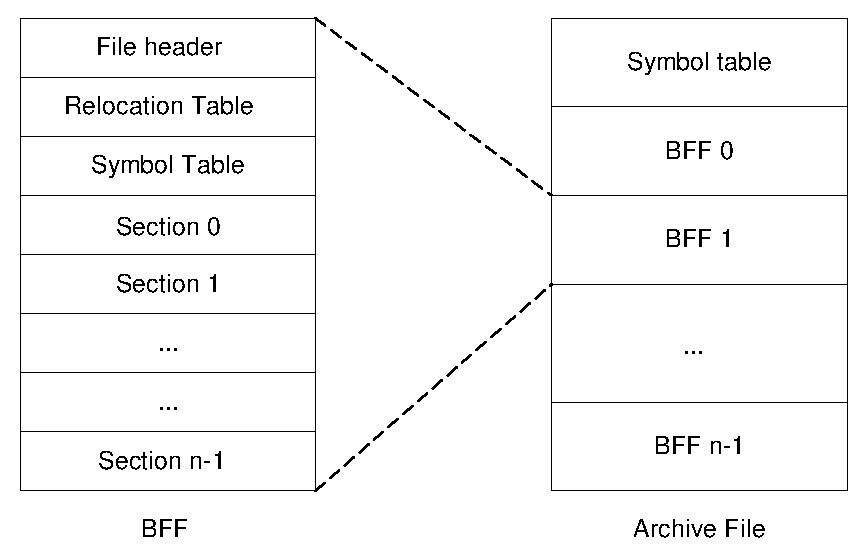
\includegraphics{figures/bffoa.eps}}
\centerfigend{fig-bffoa}{BFF and archive file abstraction}

The current development domain for our tools is based on the Solaris 
ELF~\cite{Sun94m} format, the DOS EXE format~\cite{Dunc88b,Micr96}, 
the Windows (16-bit) NE~\cite{Dunc88b,Micr96} format,
and the Palm OS .prc format~\cite{Tso00}.
Archive files are based on the Unix ar(4) file format.
These formats vary in their degree of complexity and information
stored: the DOS EXE is very simple and limited in structure,
whereas the Solaris ELF format is the most complex, while the Windows
NE is somewhere in between.
The amount of information stored for a simple ``Hello world'' program
varies from format to format.  The DOS EXE format contains a file
header, a relocation table and a single image for both code and data.
The Windows NE version contains most DOS EXE's information plus
additional details such as the resource table, entry table, etc.
The ELF format contains even more information; sections within the 
object file hold information used in dynamic linking: code, data, 
relocation tables, symbol tables, dynamic linking information, etc.
The size in bytes of the binaries for (x86,DOS,EXE), (x86,Windows,NE)
and (Sparc,Solaris,ELF) are 6432, 16384 and 5280 respectively.
It can clearly be seen that although the latter two files are dynamically
linked, their sizes are not necessarily smaller than the static (first)
case.
This is due to the small nature of the example program and the
inclusion of the DOS EXE header information within the NE format.



\section{The BinaryFile Object Hierarchy}
BinaryFile and ArchiveFile are abstract classes; that is, they cannot be
instantiated
directly. The user actually uses classes such as ElfBinaryFile or ExeBinaryFile,
which are derived from the abstract BinaryFile class (see 
Figure~\ref{fig-loadHier}).

% xfig figures exported as eps, portrait, 100% size, displayed at 3.2cm.
\centerfigbegin
\resizebox{!}{3.2cm}
{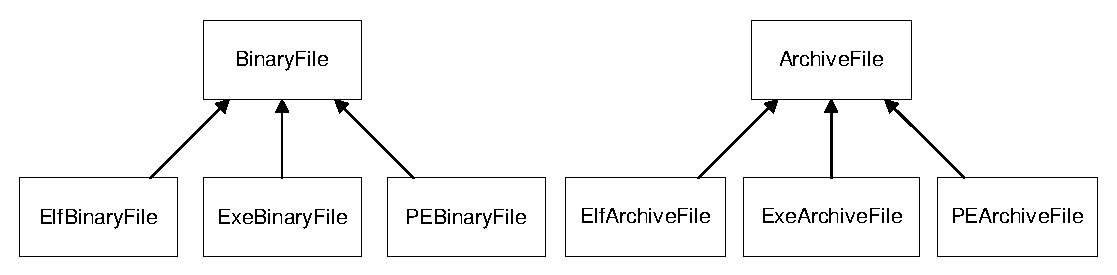
\includegraphics{figures/load_hierarchy.eps}}
\centerfigend{fig-loadHier}{BinaryFile Class Hierarchy}

The user will call functions like \texttt{Load} that are implemented 
differently in the various derived classes. Some functions like
\texttt{SymbolByAddress} are implemented trivially by the BinaryFile class 
(e.g. to always return 0), and this behaviour is overridden by derived 
classes which do the real work.  Even functions like \texttt{GetNumSyms} 
that are implemented by the BinaryFile class will return information that 
will be dependent on the instantiated class.



\section{Interface Functions to Construct and Use a BinaryFile}
The BinaryFile class and each of its parts (described in the abstract 
format description of a binary file in section~\ref{sec-bff}), are 
explained here in terms of interface functions provided for accessing 
information in those parts. 


\subsection{Construction and Loading}
The BinaryFile class provides constructor and destructor 
functions, plus a function to load the binary file.
The loader is an abstract class and hence it does not export 
any types.

\begin{description}
\item [BinaryFile: BOOL $\rightarrow$ BinaryFile].
	This is the constructor. The single BOOL argument is used to
	indicate whether the object to be constructed is to be an
	Archive member; it defaults to false. Users should not use
	this parameter, but should use the ArchiveFile class
	instead (see section~\ref{sec-archive}). The BinaryFile object
	is created without a file loaded; use the Load() function below
	to actually load a file.
	
\item [Load: (BinaryFile x STRING) $\rightarrow$ BOOL].
	Load the given file and store its
	information in a BinaryFile object. It returns whether the
	function was successful or not.
	If there is a problem loading the file, e.g. the file name does
	not exist or there is not enough memory, a message is printed
	on standard error.

\item [UnLoad: BinaryFile $\rightarrow$ nil].
	Deallocates the BinaryFile object. All information about the file
	(e.g. SectionInfo, pointers to section data) are invalid after
	calling this function.

\end{description}


\subsection{Sections}
For each section in the binary file, the following information is 
collected in a SECTIONINFO type:
\begin{itemize}
\item Section name: the name of the section, if any.  Formats like
	ELF support names for each section, such as \texttt{.text} and
    \texttt{.bss}; formats such as EXE do not provide such information
	and hence we follow the convention of naming them \texttt{\.header}
	and \texttt{.text} for the header of the file and the relocatable
	image respectively.

\item Native address: address where the section is logically loaded.
	For example, all EXE files are loaded at address 0x100000,
	representing 10:0000.  ELF files are loaded at the address
	specified in the elf file, typically 0x10000 for code and 0x20000
	for data.  The native address is typically used by diassemblers
	to give a useful address in listing. 

\item Host address: the host address is where the section is actually
	located in virtual memory, i.e. this is a pointer to the first
	byte in the section.

\item Section size: size of the section in bytes.

\item Number of entries: if the section is the equivalent to an 
	array of entries, the size of each entry is given.

\item bCode: This flag is set if the section contains executable
	instructions.

\item bData: This flag is set if the section contains data. It is possible
	for both bCode and bData to be set at the same time.

\item bBss: This flag is set if the section is not initialised, i.e. it
	is for reserving space only.

\item bReadOnly: This flag is set if the section is read only, i.e. it
	cannot be written to.

\end{itemize}

For example, with the ElfBinaryFile class, the section whose name is 
\texttt{\.rodata} would have the flags bData and bReadOnly set.
A disassembler can find all the sections worth disassembling by 
searching through all the sections for those with the flag bCode set.

Sections provide the following functions to determine the number
of sections available in the file and access its information:
\begin{description}
\item [GetNumSections: BinaryFile $\rightarrow$ int].
	Given a BinaryFile object, returns the number of sections that it 
	contains.  

\item [GetSectionInfo: (BinaryFile x int) $\rightarrow$ SECTIONINFO].
	Given an BinaryFile object and a section index, returns the information
	for that section.  Note that sections are indexed from 1.
\end{description}


\subsection{Symbol Table}
Symbol tables are often used for dynamic linking purposes, where
the names of dynamically linked-in routines are stored.  However,
sometimes program symbols are also stored in a symbol table,
whether in the same or a separate table to that of dynamic linking.

The symbol table offered by the BinaryFile class is very simple; 
there are three types of information stored for each entry:
\begin{itemize}
\item Symbol name: the symbol's name in the table.  Type: STRING.

\item Symbol address: the symbol's native address.  Type: ADDRESS.

\item Symbol size: the size in bytes associated with the symbol.
	Type: int.
\end{itemize}

The symbol table offers three access functions to its contents:
\begin{description}
\item [SymbolByAddress: (BinaryFile x ADDRESS) $\rightarrow$ STRING].
	Given a native address, returns the symbolic name associated with the 
	given native address.
	This function is useful when getting names for procedures at
	call locations.

\item [GetAddressByName: (BinaryFile x STRING) $\rightarrow$ ADDRESS].
	Given the name of a symbol, returns the native address associated
	with it.	
	If the symbol is inexistent in the symbol table, an address of 
	0 is returned.

\item [GetSizeByName: (BinaryFile x STRING) $\rightarrow$ int].
	Given the name of a symbol, returns the size in bytes of the 
	symbol, or 0 if inexistent.
\end{description}

Not all BinaryFiles provide the ByName() functions, because in some
cases the binary file format does not support it. If the functions are
not supported, they will always return 0.

Some BinaryFile classes (e.g. ExeBinaryFile) do not implement a symbol table.


\subsection{Relocation Table}
Relocation tables provide information on address that need to be
relocated prior to execution of the program.  
The advantage of knowing which addresses are relocatable is
that when decoding a machine instruction that takes an immediate
operand, we can check if this operand is an address or not. 
This provides us with useful information that is unavailable otherwise.

The functions provided to access the relocation table are:
\begin{description}
\item [IsAddressRelocatable: ADDRESS $\rightarrow$ BOOL].
	Given a native address, returns whether the address is in the
	relocation table or not.

\item [GetRelocatedAddress: ADDRESS $\rightarrow$ ADDRESS].
	Given a native relocatable address, returns the relocated 
	address for it. This function is tentative and not implemented
	as yet; RISC machines require many bit manipulations, and
	this will probably require a different interface function.
\end{description}

With object files, relocations are often associated with symbols.
Sometimes, (e.g. with GCC), intramodule function calls that
could be resolved at compile time are left until link time, so
the call has a relocation entry with an associated symbol table
entry (often not the same symbol table as the main symbols).
To make use of this, the BinaryFile provides this function:

\begin{description}
\item [GetRelocSym: ADDRESS $\rightarrow$ STRING]. Given a
native address, returns a symbol associated with the relocation
at that address, if any. If there is no symbol, the function
returns 0.
\end{description}


\subsection{Program Headers}
Application writers normally like dumping information about 
the headers of the program in order to determine format-specific
information that is not otherwise accessible via the loader
interface.  For example, a loader may have a verbose option to
display this type of information.

Unfortunately, it is difficult to provide a clean interface for
such low level details. (The previous version of the loader
attempted this, but it was not satisfactory). Therefore this
version of BinaryFile provides just one function, for dumping
all the headers in a verbose manner:

\begin{description}
\item [DisplayDetails: BinaryFile x STRING x FILE* $\rightarrow$ BOOL].
	Given a BinaryFile class and the name of the file, sends a verbose
	listing of the
	file to the file indicated by the FILE* parameter.
	The STRING parameter is merely to provide the first line of output,
	which is typically {\it Type} header for {\it Filename}.
	The FILE* parameter can be a special stream such as
	\texttt{stdio}, or a file opened with the \texttt{fopen}
	library function.

\end{description} 

The addresses referred to above are host addresses, i.e. pointers
to actual loaded data. (By contrast, native addresses are those
where part of a file is expected to be loaded in the native
operating system. Headers have no native address.

In the ElfBinaryFile, more specific functions are provided to
access different named headers, such as GetProgramHeader()
and GetSectionHeader().

Given the address of a header, an application writer would have
to know what the contents of the header looks like, and would
have to write the dump function.  We do not consider this
type of detail should be included in our BinaryFile class.


\subsection{Analysis Functions}
The following functions are provided for extra functionality 
required under binary translation, they are:
\begin{description}
\item [GetInitialState: BinaryFile $\rightarrow$ LIST$<$(REGxADDRESS)$>$].
	Returns a list of registers and their initial value (normally
	an address) prior to program execution.

\item [GetEntryPoints: BinaryFile $\rightarrow$ LIST$<$ADDRESS$>$].
	Returns a list of native addresses which are entry points into the 
	program.  The first address is always the initial value of the program
	counter (PC).

\emph{The following function is not implemented at present. It occured to
	me (Mike) that
	the mapping from Native to Host address may vary for each section;
	it doesn't in elf, but it may for other sections. Let's leave this
	one out unless we really need it. It is easy to implement anyway:
	just use the difference between native and host addresses in the
	section info.}
\item [NativeToHostAddress: (BinaryFile x ADDRESS) $\rightarrow$ ADDRESS].
	Given a native address, returns its equivalent host address.
	This function allows access to a block of bytes, since a native
	address is just a pointer.

\item [IsDynamicLinkedProc: (BinaryFile x ADDRESS) $\rightarrow$ BOOL].
	Given a native address, returns whether the address is that of a 
	dynamically linked-in procedure or not in this BinaryFile class.

\item [LoadDynamicLinkedProc: BinaryFile $\rightarrow$ ADDRESS $\rightarrow$ BOOL].
	Given the address of a dynamically linked-in procedure (i.e. the
	target of a call instruction that calls such a function, which
	will usually be an address in the Program Linkage Table), loads
	the appropriate source library file (if needed) to resolve this
	call. It returns its success or otherwise, and the native address
	where the procedure is loaded. 

	There will have to be environment variables to specify what path(s)
	should be searched to locate the appropriate library. These would
	be called \\
	X86\_LIBRARY\_PATH\\
	SPARC\_LIBRARY\_PATH\\
	and so on.  For example,
	if an X86 source program calls the \texttt{atan} function,
	the program's dynamic section specifies the DT\_NEEDED libraries
	as "libc.so.1" and "libm.so.1", and the environment variable
	X86\_LIBRARY\_PATH is set to "/var/lib/x86:/usr/lib/x86", then
	the following libraries will be searched for the \texttt{atan}
	function: \\
	/var/lib/x86/libc.so.1, /var/lib/x86/libm.so.1,
	/usr/lib/x86/libc.so.1, /usr/lib/x86/libc.so.1 \\
	Note that this function is only needed if/when we start supporting
	translations of libraries; at present we assume a native library
	is available.  Hence this function is not implemented at present.
\end{description}



\section{Notes on Individual BinaryFiles}

At present, the ElfBinaryFile is by far the most complete. It is the
only version that implements DisplayDetails(). The need to use
ElfDetails.cc at all, and all the verbose dumping code, can be 
avoided by defining \texttt{NODETAILS} in the make.

The ExeBinaryFile class does not handle symbols (e.g. Microsoft
Codeview or Borland) as these are stored in different ways by
different EXE compilers.

ElfBinaryFile implements symbols, both by address and by name. The
table of symbols looked up by value comes from the \texttt{.symtab}
section, if present, otherwise from the \texttt{.dynsym} section.

When looking up symbols by name, the \texttt{.hash} section is used. This
section refers to the \texttt{.dynsym} section, not the \texttt{.symtab}
section (if present). 
Thus, it is possible to look up local (non dynamic) symbols by value, 
but not by name.  This is a limitation of the way that elf files
are made. 
ElfBinaryFile implements the symbol size field of the SYM\_VALUE passed to 
ValueByName().

Some library files (e.g. libstdc++) have silly dynamic symbol table
entries (that they don't define), with a symbol type of STT\_NOTYPE.
Symbols of this kind are treated as if they don't exist in the symbol
table (i.e. ValueByName() returns 0 for these). 



\section{Interface Functions to Construct and use an ArchiveFile}
\label{sec-archive}

The ArchiveFile class and each of its parts (described in the abstract 
format description of a binary file in section~\ref{sec-bff}), are 
explained here in terms of interface functions provided for accessing 
information in those parts. 

\begin{description}
\item [ArchiveFile: nil $\rightarrow$ ArchiveFile].
	This is the constructor; there are no arguments. The object is
	created without a file being loaded; use the Load function below
	to load an archive file.

\item [Load: STRING $\rightarrow$ BOOL].
	Loads the archive file whose name is given. Returns false if the
	file could not be found, not opened, or it was not an archive
	file. Messages may be displayed on standard error.

\item [UnLoad: ArchiveFile $\rightarrow$ nil].
	Unloads the archive file, and any members that may have been loaded
	and not yet unloaded.  All information about the archive file
	and member files are invalid after calling this function.

\item [GetNumMembers: ArchiveFile $\rightarrow$ int].
	Returns the number of members, not including any special members
	that may exist merely for administrative purposes (e.g. the
	empty members in elf archives that hold the symbol table).

\item [GetMember: ArchiveFile x int $\rightarrow$ BinaryFile*].
	Given an index (0 for first, etc), constructs, loads, and returns
	a pointer to a BinaryFile object for that member. The binaryfile
	object comes pre-loaded; the user should not call the Load function
	for the returned member, but should call UnLoad when done with the
	member object. In the case of errors, a NULL pointer is returned.

\item [GetMemberByProcName: ArchiveFile x STRING $\rightarrow$ BinaryFile*].
	Similar to the above function, except that the relevant member is
	selected by procedure name, e.g. "arctan".

\item [GetMemberByFileName: ArchiveFile x STRING $\rightarrow$ BinaryFile*].
	Similar to the above function, except that the relevant member is
	selected by the name of the archive member (this will usually be an
	object file without an explicit path, e.g. "transcend.o").

\item [GetMemberFileName: ArchiveFile x int $\rightarrow$ STRING].
	Given a member index, return the name of the archive member.


\end{description}

Many of the functions above presume some knowledge of the contents of
the archive, e.g. the file name of the members, or symbols in those
members. There are at present no functions to allow the user to browse
these items.

\section{Example Code}

Examples are often worth a thousand words.  Here are two examples
on how to use the BinaryFile and derived classes.


\subsection{Example 1}
Here is a complete, though simple, program to use the ElfBinaryFile class. 
It simply iterates through the sections of the file, and counts how 
many sections contain code (i.e.  have the ST\_CODE flag set).

\begin{verbatim}
#include <stdio.h>
#include "ElfBinaryFile.h"

int main(int argc, char* argv[])
{
    ElfBinaryFile L;
    int iCnt = 0;

    if (!L.Load(argv[1])) return 1;
    int n = L.GetNumSections();
    PSECTIONINFO pSect = L.GetSectionInfo();
    for (int i=0; i < n; i++)
        if (pSect[i].bCode) iCnt++;
    printf("Part %d has %d code section(s)\n", iPart, iCnt);
    L.UnLoad();
    return 0;
}
\end{verbatim}

This can be compiled as follows (assuming that the above source is in
\texttt{sample.cc}):
\begin{verbatim}
gcc -o sample sample.cc BinaryFile.cc ElfBinaryFile.cc ElfDetails.cc
    SymTab.cc -lelf -lstdc++
\end{verbatim}

The \texttt{"-lelf"} is because ElfBinaryFile requires the elf library; other
versions of the loader would probably not need any libraries other than the
standard template library.
The results are:

\begin{verbatim}
% sample sample
Part 1 has 4 code section(s)

% sample /usr/lib/libelf.a
Part 1 has 1 code section(s)
Part 2 has 1 code section(s)
...
Part 42 has 1 code section(s)
\end{verbatim}


\subsection{Example 2}
The following example dumps the \texttt{\_exit} function
(if present) of the given input file.   Assume the following
code is in file dumptext.cc.

\begin{verbatim}
#include "ElfBinaryFile.h"

int main(int argc, char* argv[])
{
    ElfBinaryFile L;
    SYM_VALUE v;
    PSECTIONINFO pText;

    if (!L.Load(argv[1])) return 1;

    if (L.ValueByName("_exit", &v))
    {
        pText = L.GetSectionInfoByName(".text");
        if (pText)
        {
            int n = v.iSymSize;
            printf("Function _exit (%d bytes):\n", n);
            printf("%08X: ", pText->uNativeAddr);    // Address
            // Compute offset from start of text section to this function
            dword offset = v.uSymAddr - pText->uNativeAddr;
            dword p = pText->uHostAddr + offset;    // Start of function
            for (int i=0; i < n; i++)
                printf("%02X", *((unsigned char*)p++));
            printf("\n");
        }
    }
    else printf("No function '_exit'\n");
    return 0;
}
\end{verbatim}

To compile it, at the command line type:
\begin{verbatim}
gcc -g -o dumpexit dumpexit.cc BinaryFile.cc ElfBinaryFile.cc SymTab.cc 
    ElfDetails.cc -lelf -lstdc++
\end{verbatim}

Sample output: 
\begin{verbatim}
% dumpexit /usr/lib/libc.so.1 
Function _exit (8 bytes):
000169A0: 8210200191D02008
% 
\end{verbatim}

\subsection{Example 3}

The following example loads the archive "/usr/lib/libm.a" and displays
the load address for the "sin" function.

\begin{verbatim}
#include <stdio.h> 
#include "ElfArchiveFile.h"
void main()
{

    ElfArchiveFile af;
    if (!af.Load("/usr/lib/libm.a"))
    {
        printf("ArchiveFile could not load file\n");
        return 1;
    }

    printf("There are %d members in this archive\n", af.GetNumMembers());
    printf("First 5 file names:\n");
    for (int i=0; i < 5; i++)
    {
        printf("%s\n", af.GetMemberFileName(i));
    }

    BinaryFile* pm;
    printf("Object for function 'sin' is at %p\n",
        pm = af.GetMemberByProcName("sin"));
    printf("Address of sin is %p; size %d\n", pm->GetAddressByName("sin"),
        pm->GetSizeByName("sin"));
    pm->UnLoad();

	af.UnLoad();
}
\end{verbatim}

To compile, (assuming the example code is called example3.cc):
\begin{verbatim}
gcc -g -DUNIX -o example3 example3.cc BinaryFile.cc ElfBinaryFile.cc
    SymTab.cc ElfDetails.cc ArchiveFile.cc ElfArchiveFile.cc -lelf -lstdc++
\end{verbatim}


\subsection{Compiling and Linking}
Applications using the BinaryFile class need to compile the files 
\texttt{BinaryFile.cc} and \texttt{ExeBinaryFile.cc} (or \texttt{ElfBinaryFile.cc},
\texttt{PEBinaryFile.cc}, etc).  They should link the resultant object files 
with the application. The final executable must be linked with the standard
template library, e.g. "-lstdc++" for the GCC compiler. Elf versions
also require the elf library, i.e. "-lelf" for GCC.

In addition, BinaryFile classes implementing symbol tables (at present,
this is only the ElfBinaryFile class) also need to compile \texttt{SymTab.cc}
which depends on \texttt{SymTab.h}, and should link with \texttt{SymTab.o}.

For the ElfBinaryFile class, unless \texttt{NODETAILS} is defined in
the make (with \texttt{-DNODETAILS}), the file \texttt{ElfDetails.cc}
must also be compiled and the resultant \texttt{ElfDetails.o} linked.

In those application source files using the BinaryFile class, the appropriate
header file (but not \texttt{BinaryFile.h} itself) should be included. For
example, if using ElfBinaryFile:
\begin{verbatim}
#include "ElfBinaryFile.h"		// Definitions for the ElfBinaryFile class
\end{verbatim}

An example makefile fragment:
\begin{verbatim}
OBJS = myfile1.o ... BinaryFile.o ElfBinaryFile.o SymTab.o ElfDetails.o

ElfBinaryFile.o: BinaryFile.o ElfBinaryFile.h ElfDetails.h

SymTab.o: SymTab.cc SymTab.h

BinaryFile.o: BinaryFile.h
\end{verbatim}



       % binary-file API 

	
\chapter{Decoding of Machine Instructions -- Syntax Parsing}
\label{ch-decoding}

{\small
\begin{flushright}
Design: Cristina; Documentation: Cristina [Feb 00]; Implementation: Cristina, Mike
\end{flushright} 
}


The New Jersey Machine Code (NJMC) toolkit allows users to write
machine descriptions of assembly instructions and their associated
binary representations using the Specification Language
for Encoding and Decoding (SLED).
SLED provides for compact specifications of RISC and CISC 
machines; with 127, 193 and 460 lines of specification for
the MIPS, SPARC and Pentium respectively. 

The toolkit also provides extra support for encoding of assembly to
binary code, and decoding of binary to assembly code.
For decoding purposes, the toolkit provides a \emph{matching} statement 
which resembles the C \texttt{switch} statement.  
The toolkit generates C and Modula-3 code from matching statements, 
hence automating part of the disassembly process.  
The generated code can be integrated as a module of a binary-decoding 
application.  This chapter briefly describes the SLED language, its usage 
for decoding of machine instructions, and the way we have optimised the 
the code that the toolkit generates.


\section{SLED and Decoding of Machine Instructions}
This section provides a brief description of the SLED language in 
order to familiarize the reader with the key concepts of the language.
Readers familiar with the toolkit and its usage should skip this section. 
A full description of the SLED language is provided in~\cite{Rams97}.
A complete description of the usage of the toolkit for both
encoding and decoding purposes is available in the reference 
manual~\cite{Rams94}.


\subsection{SLED Concepts}
SLED introduces the following concepts to describe binary machine
instructions:
\begin{description}
\item [tokens] represent names for a sequence of bits.  Tokens are 
	commonly used to represent the bits of one machine instruction
	or of immediate operands.  A token is given a size, representing
	the number of bits in the token.
\item [fields] describe the parts of a token in terms of their name
	and bit range.  Fields can use little or big endian conventions.
\item [patterns] describe the possible values in the fields of
	a token, and names them.  Pattern names can also refer to groups
	of patterns.
\item [constructors] describe the mapping between binary and a
	symbolic assembly-like representation by associating 
	a list of operands with a pattern.
\item [equations] describe simple mathematical equations which
	place constraints on the values of fields used in constructors.
\item [relocatables] describe operands in constructors that denote 
	relocatable addresses.
\end{description}

A partial example of the SPARC SLED specification is given in
Figure~\ref{fig-sparc-sled}.
The \texttt{fields} keyword describes the specification of
a token named \texttt{instruction} of size 32 bits.  The fields
of that token include: \texttt{op}, \texttt{rd}, and \texttt{rs1}. 
Each field denotes a sequence of bits of the \texttt{instruction} 
token it refers to. 
For example, the \texttt{op} field refers to bits 30 and 31, and
the \texttt{rs1} field refers to bits 14 to 18.   
By default, big-endian convention is used.

\centerfigbegin
\begin{small} 
\begin{verbatim}
fields of instruction (32)
inst 0:31 op 30:31 disp30 0:29 rd 25:29 op2 22:24 imm22 0:21 a 29:29 cond 25:28
disp22 0:21 op3 19:24 rs1 14:18 i 13:13 asi 5:12 rs2 0:4 simm13 0:12 opf 5:13
fd 25:29 cd 25:29 fs1 14:18 fs2 0:4 rs1i 14:18 rdi 25:29

patterns
 [ TABLE_F2 CALL TABLE_F3 TABLE_F4 ] is op  = {0 to 3}
patterns
 [ ADD  ADDcc  TADDcc   WRxxx
   AND  ANDcc  TSUBcc   WRPSR
   OR   ORcc   TADDccTV WRWIM
   XOR  XORcc  TSUBccTV WRTBR
   SUB  SUBcc  MULScc   FPop1
   ANDN ANDNcc SLL      FPop2
   ORN  ORNcc  SRL      CPop1
   XNOR XNORcc SRA      CPop2
   ADDX ADDXcc RDxxx    JMPL
   _    _      RDPSR    RETT
   UMUL UMULcc RDWIM    Ticc
   SMUL SMULcc RDTBR    FLUSH
   SUBX SUBXcc _        SAVE
   _    _      _        RESTORE
   UDIV UDIVcc _        _
   SDIV SDIVcc _        _       ] is TABLE_F3 & op3 = {0 to 63 columns 4}
patterns
  arith   is ADD | ADDcc | ADDX | ADDXcc | TADDcc | TADDccTV |
             SUB | SUBcc | SUBX | SUBXcc | TSUBcc | TSUBccTV |
             MULScc | UMUL | SMUL | UMULcc | SMULcc |
             UDIV | SDIV | UDIVcc | SDIVcc | SAVE | RESTORE

constructors
  imode simm13! : reg_or_imm  is  i = 1 & simm13
  rmode rs2     : reg_or_imm  is  i = 0 & rs2
constructors
  arith rs1, reg_or_imm, rd
relocatable reloc
constructors
  call reloc   { reloc = L + 4 * disp30! } is L: CALL & disp30
\end{verbatim}
\end{small}
\centerfigend{fig-sparc-sled}{Partial SLED specification for the SPARC}

The first \texttt{patterns} keyword defines names for 4 patterns: 
\texttt{TABLE\_F2}, \texttt{CALL}, \texttt{TABLE\_F3}, and 
\texttt{TABLE\_F4}.  Each of these patterns bind to a value of
the \texttt{op} field: \texttt{TABLE\_F2} binds to 0, \texttt{CALL}
binds to 1, \texttt{TABLE\_F3} binds to 2, and \texttt{TABLE\_F4} binds
to 3.  In this way, the 4 main tables described in the SPARC 
manual~\cite{Spar92} can be identified.
The second \texttt{patterns} keyword defines names for each of
the 64 values that the combination of the \texttt{TABLE\_F3} pattern
(i.e. \texttt{op} equal to 2) and the field \texttt{op3} can take.  
Entries labelled \texttt{\_} denote entries without a name; i.e. 
entries that are not defined in the manual.   
The third \texttt{patterns} keyword defines the name \texttt{arith} 
to be any of the patterns in the right-hand side of the \texttt{is} 
keyword; namely \texttt{ADD}, \texttt{ADDcc}, \texttt{TADDcc}, etc.

The first \texttt{constructor} keyword defines the constructor
\texttt{reg\_or\_imm} to be one of two modes: immediate (\texttt{imode})
or register-based (\texttt{rmode}).  The former mode binds 
the value of the \texttt{i} field to 1, and the latter to 0.
The former mode returns the 13-bit value \texttt{simm13} signed-extended 
(the \texttt{!} denotes sign-extension), whereas the latter mode
returns the value of the \texttt{rs2} field (a register number).
The second \texttt{constructor} keyword defines the constructor
\texttt{arith} to require the fields and constructors \texttt{rs1}, 
\texttt{reg\_or\_imm}, and \texttt{rd} (which stand for first register 
operand, second register or immediate operand, and destination register). 
In this definition, it is implied that the bit pattern to be 
matched is that of the pattern \texttt{arith} and the fields
\texttt{rs1}, \texttt{reg\_or\_imm}, and \texttt{rd}.  In other
words, this constructor defines all the arithmetic instructions for
the SPARC. 
The last \texttt{constructor} keyword defines the constructor
\texttt{call}, which takes a relocatable address (denoted by
\texttt{reloc}).  The relocatable address needs to satisfy the
equation \texttt{reloc = L + 4 * disp30!}. 
That is, the relocatable address is equivalent to the sign-extended
(\texttt{!}) 30-bit displacement (\texttt{disp30}) shifted left by 2 
(i.e. a 32-bit address where the least two significant bits are 0) plus 
the current displacement (\texttt{L}).  The value of \texttt{L} is
obtained at runtime, by checking the address at which the 
\texttt{CALL} bit pattern is being decoded from.  The \texttt{call}
constructor is defined as the bit pattern combination of the 
\texttt{CALL} pattern and the \texttt{disp30} field.


\subsection{Decoding Using the New Jersey Machine Code Toolkit}
The NJMC toolkit uses matching statements to drive the decoding
of a binary instruction stream.  A matching statement resembles
a C \texttt{switch} statement, except that only one arm can 
be matched (the first one to be valid in the instruction 
stream). 
A matching statement is identified by the \texttt{match}
keyword.  Arms of the match are identified by the \texttt{|} symbol, 
and the left and right-hand sides of the arm are separated by the 
\texttt{=>} symbol. 
Figure~\ref{fig-matching} provides an EBNF-like specification of
the matching statement.  In that specification, \emph{pc} stands 
for the address to the instruction stream to be decoded, 
\emph{pattern} stands for the SLED pattern to be matched 
(including parameters), \emph{equation} stands for any valid
SLED equation that needs to be valid in conjunction with a 
particular pattern, and \emph{code} stands for the C or Modula3
code that the user wants to associate with the matched pattern.
The keyword \texttt{[name]} is used to return the SLED base
pattern name for the matched pattern. 

\begin{figure}[htb]
\texttt{match} pc \texttt{to} \\
\{\texttt{|} pattern [\{equations\}] [\texttt{[name]}] \texttt{=>} code \} \\
{[\texttt{else} code]} \\
\texttt{endmatch}
{\small \caption{\label{fig-matching}{Matching Statement EBNF Specification}}}
\end{figure}
  
For example, if the patterns \texttt{add} and \texttt{sub} are 
described in a SLED specification for a particular machine, then 
the following matching statement displays those names when matched 
at the binary instruction stream pointed to by the address in \texttt{pc}:
\begin{verbatim}
match pc to
| add (rd, rs1, rs2) => printf ("add\n");
| sub (rd, rs1, rs2) [name] => printf ("%s\n", name);
| else                  printf ("other instruction\n");
endmatch
\end{verbatim}

The ``arguments'' to the constructor are names that match
the field names defined with each constructor (in order of
specification) and return the numerical value of
that field.  Hence, in the above example, \texttt{rd}, 
\texttt{rs1} and \texttt{rs2} are integers.  An application
writer may want to give special semantics to such returned
integers; for example, displaying the name of the register
instead of the integer representation of the register.  If
we assume we have an array of register names called \texttt{reg},
the above example can be re-written to also display the names of the
arguments:
\begin{verbatim}
match pc to
| add (rd, rs1, rs2) => printf ("add %s, %s, %s\n", reg[rd], reg[rs1], reg[rs2]);
| sub (rd, rs1, rs2) [name] => 
                        printf ("%s %s, %s, %s\n", name, reg[rd], reg[rs1], reg[rs2]);
| else                  printf ("other instruction\n");
endmatch
\end{verbatim}

Matching files are processed by the toolkit to generate C or 
Modula-3 code that implements the decoding of the instructions
in the \texttt{match} statement.  

Version 0.5 of the NJMC toolkit makes available an option to
partly automate the generation of a matching statement for a
particular SLED specification.  The option \texttt{-dis} generates
matching statements for the given SLED file(s) and stores them 
in the filename provided:  \\
\hspace*{2cm}\texttt{-dis} filename sledfile(s)\\
In practice, the generated code needs to be modified in order to add 
relevant procedure names for each main matching statement, 
as well as remove duplicated arms from the matching statements.
Note that this option is not currently available in the ML 
version of the toolkit.


\subsubsection{Decoding of RISC Machine Instructions}
Some of the characteristics of RISC machines include the 
orthogonality of their instruction sets and the relatively 
small number of instructions.  Further, the size of each
instruction is fixed and is equivalent to the word size 
of the machine.  These characteristics make the writing
of a SLED spec and decoder easier than for a CISC instruction
set.

Figure~\ref{fig-sparc-decoder} contains a snippet of code
for the SPARC decoder; this code was written by hand rather
than generated automatically.  The main decoding routine is 
\texttt{decode\_instr}, which decodes one instruction per
invocation.  The \texttt{pc} argument points to the address
in memory where the instruction stream to be decoded is located
at.  The \texttt{uNativeAddr} argument contains the native
address where the Elf Loader would be expected to load the
instruction stream, and the \texttt{buf} argument is a buffer
where the textual assembly representation of this instruction
will be stored.  The code in this procedure is straight 
forward, except for the target address of branches and calls.
Other than the type name \texttt{ADDRESS}, all names in uppercase 
represent macros used as a shorthand for invoking functions or 
accessing arrays of strings.

Constructors for branches and calls are defined in the SLED 
spec as using relocatable addresses.  Therefore, the toolkit
generates code to return the relocated target address rather
than the original offset displayed in the instruction.  However,
due to the fact that the toolkit is using the \texttt{pc} address
as the address to relocate from, rather than the \texttt{uNativeAddr}
which it does not know about, the returned target address is 
wrong; hence the use of a simple equation to transform the target
address to the right one.   

\centerfigbegin
{\small
\begin{verbatim}
#define RD   (rd_names[rd])
#define RS1  (rs1_names[rs1])
#define ROI  (dis_roi(roi))
#define ADDR (dis_addr(addr))

char *dis_addr(ADDRESS lc) {
  static char buf[512];
  match lc to
  | indirectA(rs1)   => return RS1;
  | indexA(rs1, rs2) => sprintf(buf, "%s+%s", RS1, RS2);
  | absoluteA(i)     => sprintf(buf, "%d", i);
  | dispA(rs1, i)    => sprintf(buf, "%s%s%d", RS1, (int)i < 0 ? "" : "+", i);
  endmatch
  return buf;
}

char *dis_roi(ADDRESS lc) {
  static char buf[512];
  match lc to
  | imode(i)   => sprintf(buf, "%d", i); return buf;
  | rmode(rs2) => return RS2;
  endmatch
}

void decode_instr (ADDRESS pc, ADDRESS uNativeAddr, char *buf)
{
  match pc to
  | NOP =>          sprintf(buf, "nop");
  | decode_sethi(imm22, rd) =>
                    sprintf(buf, "sethi %%hi(%s), 0x%x", imm22, RD);
  ...
  | alu (rs1, roi, rd) [name] =>
                    sprintf(buf, "%s %s, %s, %s", name, RS1, ROI, RD);
  | branch^a (tgt, a) [name] =>
                    sprintf(buf, "%s 0x%08x (%d) ; a = %d", name,
                           tgt-pc+uNativeAddr, tgt-pc, a);
  | call (tgt) =>   sprintf(buf, "call 0x%08x", tgt-pc+uNativeAddr);
  | JMPL (addr, rd) [name] =>
                    sprintf(buf, "jmpl %s, %s", ADDR, RD);
  ...
  | inst = n =>     sprintf(buf, ".word 0x%08x", n);
  endmatch        
\end{verbatim}
}
\centerfigend{fig-sparc-decoder}{Snippet Code for a SPARC Decoder}

The functions \texttt{dis\_addr} and \texttt{dis\_roi} implement
the matching of an effective address, and a register or immediate 
operand, respectively.  
In the former function, an effective address is defined as being
one of 4 cases, namely, indirect, indexed, absolute, or displacement.
In the latter function, a register or immediate is either of those
two options, which can also be matched against the SLED spec.
Both functions return a buffer with the assembly version of 
the bits matched.

The toolkit provides support for generating the names of registers
based on the names used for patterns in the SLED spec.  In a SLED
spec, any name values given for fields with the \texttt{fieldinfo}
keyword can be retrieved automatically by the toolkit in an array 
of strings.  The command line option \\
\hspace*{2cm}\texttt{-lc-pat-names} \\
generates a header and data declaration file (.h and .c) with the
names of all strings found in a SLED spec.  In our previous 
example, the names for \texttt{rs1\_names} and \texttt{rd\_names} 
were generated by the toolkit in a separate file and imported into
the decoder (aka matcher) file.

In order for the toolkit to fetch instructions from the bit stream
addressed by \texttt{pc} in the previous example, a fetch routine
needs to be provided by the tool writer.  In the case of SPARC, 
all fetches will be 32 bits as all instructions are 32 bits, hence
a \texttt{fetch\_word} function needs to be made available.  Suitable
code for such a function is:
\begin{verbatim}
static ADDRESS fetch_word(ADDRESS lc) {
  return *(ADDRESS *)lc;
}
\end{verbatim}
where \texttt{ADDRESS} is a 32-bit type.  Information about the name
of this function, the type of the address field, and address 
conversions need to be specified in an auxiliary spec.  For the 
SPARC decoder, the interface to the instruction stream is as 
follows:
\begin{verbatim}
address type is "unsigned"
address to integer using "%a"
address add using "%a+%o"
fetch 32 using "fetch_word(%a)"
\end{verbatim} 

Norman believes that in order to get the right relocated address 
out of branches and calls, that the \texttt{address to integer} 
option needs to be changed to something like this: \\ 
\hspace*{2cm}\texttt{address to integer using "\%a - uNativeAddr + pc"} \\
In practice, this has not worked yet, and I have not tried it lately.


\subsubsection{Decoding of CISC Machine Instructions}
Amongst the characteristics of CISC machines are the lack of 
orthogonality in their instruction sets, the large numbers of
machine instructions, and the variable length size for 
instructions.  Further, assembly names are often overloaded.
These characteristics make the writing of SLED specs for CISC
machines harder; nevertheless, the language is expressive 
enough.  

Figure~\ref{fig-cisc-sled} contains part of the SLED code for
the x86 instruction set.  The complexity of the instruction 
set can be seen in terms of the number of different \texttt{field}
definitions, the complex names used to distinguish overloaded
instruction names, and the variety of values available on the
right hand side of constructors.  Further, the addressing modes
(\texttt{Eaddr} and \texttt{Mem}) account for 10 possible 
combinations.

\centerfigbegin
{\small
\begin{verbatim}
fields of opcodet (8) row 4:7 col 0:2 page 3:3
    sr4 3:5 sr16 0:2 r16 0:2 r8 0:2
fields of modrm (8) mod 6:7 reg_opcode 3:5 r_m 0:2
fields of I8   (8) i8  0:7

patterns
arith is any of [ ADD OR
                  ADC SBB
                  AND SUB
                  XOR CMP ], which is row = {0 to 3} & page = [0 1]
[ Eb.Gb Ew.Gw Gb.Eb Gw.Ew AL.Ib AX.Iw ] is col = {0 to 5}

patterns
  arithI    is any of [ ADDi ORi ADCi SBBi ANDi SUBi XORi CMPi ],
            which is (Eb.Ib | Ew.Iw | Ew.Ib); reg_opcode = {0 to 7} ...

relocatable d a
constructors
  Indir    [reg] : Mem { reg != 4, reg != 5 } is mod = 0 & r_m = reg
  Disp8   d[reg] : Mem { reg != 4 }           is mod = 1 & r_m = reg; i8  = d
  Disp32  d[reg] : Mem { reg != 4 }           is mod = 2 & r_m = reg; i32 = d
  Abs32   a      : Eaddr                      is mod = 0 & r_m = 5;   i32 = a
  Reg     reg    : Eaddr                      is mod = 3 & r_m = reg
  Index    [base][index * ss] : Mem { index != 4, base != 5 } is
                        mod = 0 & r_m = 4; index & base     & ss
  Index8  d[base][index * ss] : Mem { index != 4 } is
                        mod = 1 & r_m = 4; index & base     & ss; i8  = d
  Index32 d[base][index * ss] : Mem { index != 4 } is
                        mod = 2 & r_m = 4; index & base     & ss; i32 = d
  ShortIndex    d[index * ss] : Mem { index != 4 } is
                        mod = 0 & r_m = 4; index & base = 5 & ss; i32 = d
  E Mem : Eaddr is Mem

constructors
  arith^"iAL"    i8           is      arith & AL.Ib ; i8
  arith^"iAX"    i16          is      arith & AX.Iw; i16
  arith^"mrb"    Eaddr, reg8! is      arith & Eb.Gb; Eaddr & reg_opcode = reg8 ...
  arith^"mrw"    Eaddr, reg!  is      arith & Ew.Gw; Eaddr & reg_opcode = reg ...
  arith^"rmb"    reg8!, Eaddr is      arith & Gb.Eb; Eaddr & reg_opcode = reg8 ...
  arith^"rmw"    reg!, Eaddr  is      arith & Gw.Ew; Eaddr & reg_opcode = reg ...
  arithI^"wb"    Eaddr, i8!   is      (Ew.Ib; Eaddr) & arithI; i8
  arithI^"b"     Eaddr, i8    is      (Eb.Ib; Eaddr) & arithI; i8
  arithI^"w"     Eaddr, i16   is      (Ew.Iw; Eaddr) & arithI; i16
\end{verbatim}
}
\centerfigend{fig-cisc-sled}{Partial SLED Spec for the x86 Instruction Set}

The partial decoder in Figure~\ref{fig-cisc-decoder} illustrates
matching statements used to decode the x86 instruction set.
The code was mostly generated automatically by the toolkit, with 
manual editing performed in order to remove redundant arms from the 
matching statements, separation of nesting of matching statements, and 
creation of function prototypes.
The matching statement for \texttt{decode\_instr} makes use of 
the optional \texttt{[deltaPC]} notation, the effect of which
is to store the number of bytes that were parsed in the \texttt{deltaPC}
variable.  This is needed by a decoder of CISC instructions as
the instruction length is variable and a multiple of 1 byte.
In the code provided, the address of the host instruction stream
and that of the native address are given in 32-bit quantities, 
which means that 4 bytes can potentially be fetch, although any
one particular instruction may only be 1 or 2 bytes.  We use the
returned \texttt{deltaPC} value to update the host pointer by 
the necessary amount.

Characteristics of the generated code include the abstraction 
of the assembly print and file descriptor used---\texttt{asmprint}
and \texttt{asmprintfd} respectively.  These can be defined in
any suitable way in the tool writer's code; in our case, we defined
them as \texttt{fprintf} and \texttt{stdout} respectively.
The toolkit also generates functions to print signed and unsigned
integer values, dependeing on their size; for example, 
\texttt{print\_signed\_i8} to print an 8-bit signed integer. 
Functions to print registers may depend on the context of 
the instruction; i.e. the register number may be that of a 
byte, 2-byte or 4-byte register, which equates to different 
ascii representation of registers (e.g. \texttt{AL} or \texttt{AX}
or \texttt{EAX}).  In this case, the toolkit generates code to
print the decimal value of the register (i.e. 1, 2 or 4).  
I modified this function manually to display 32-bit registers 
for disassembly purposes -- this code is not correct for all
cases and can be corrected by passing an extra argument to the
print function with the size of the register operand.  
    
\centerfigbegin
{\small
\begin{verbatim} 
#define asmprintf fprintf   // printf function
#define asmprintfd stdout   // print directly to stdout

static void print_Eaddr (unsigned pc) {
    match pc to
    | Abs32 (a) =>
            asmprintf (asmprintfd, "%d", a);
    | E (mem) =>
            print_Mem (mem);
    | Reg (reg) =>
            asmprintf (asmprintfd, "%s", print_unsigned_r32(reg));
    endmatch
}

static void print_signed_reg(int reg) { 
  static char *r32_names[] = {
    "EAX", "ECX", "EDX", "EBX", "ESP", "EBP", "ESI", "EDI",
  };
  asmprintf(asmprintfd, "%s", r32_names[reg]);
//  asmprintf(asmprintfd, "%d", reg);
}

static void print_signed_i8(int /* [-128..127] */ i8) {
  asmprintf(asmprintfd, "%d", i8);
}

unsigned decode_instr (unsigned pc, unsigned uNativeAddr)
{ unsigned deltaPC;     // # of bytes parsed by decoder

  match [deltaPC] pc to
  | ADDrmw(reg, Eaddr) =>
      asmprintf(asmprintfd, "%s", "ADDrmw ");
      print_signed_reg(reg);
      asmprintf(asmprintfd, "%s", ", ");
      print_Eaddr(Eaddr);
  | ADDrmb(reg8, Eaddr) =>
      asmprintf(asmprintfd, "%s", "ADDrmb ");
      print_signed_reg(reg8);
      asmprintf(asmprintfd, "%s", ", ");
      print_Eaddr(Eaddr);
      asmprintf(asmprintfd, "\n");
  | ADDiw(Eaddr, i16) =>
      asmprintf(asmprintfd, "%s", "ADDiw ");
      print_Eaddr(Eaddr);
      asmprintf(asmprintfd, "%s", ", ");
      print_signed_i16(i16);
  | ADDiAL(i8) =>
      asmprintf(asmprintfd, "%s", "ADDiAL ");
      print_signed_i8(i8);
      asmprintf(asmprintfd, "\n");
  ...
  endmatch
  return deltaPC;
}
\end{verbatim}
}
\centerfigend{fig-cisc-decoder}{Snippet Code for an x86 Decoder}

For CISC machines, the toolkit will need to fetch bits in different
byte granularities.  For x86, 1, 2 or 4 bytes may need to be fetched
at any point in time.  This information, along with address information,
is stored in the instruction stream interface file, as follows:
\begin{verbatim}
fetch 8 using "getByte(%a)"
fetch 16 using "get2Bytes(%a)"
fetch 32 using "get4Bytes(%a)"
address type is "unsigned"
address add using "(unsigned)%a + %o"
address to integer using "%a"
\end{verbatim}
And the user is required to provide the implementation for the
functions \texttt{getByte}, \texttt{get2Bytes} and \texttt{get4Bytes}.


\subsection{Cost of Decoding Machine Instructions}
\emph{Some experimentation in this area was done in 
1998 in order to determine bottlenecks in the generated
code and store it in a different way.  The work was 
never finished and neither Norman nor Cristina had
the time to make changes.}

The current NJMC implementation for generating C code from 
matching files is to use a decision tree for all options 
available in a \texttt{match} statement.  In these decision 
trees, every option is inline expanded.  The tree is then
turned into a DAG and only at leaf nodes are \texttt{goto}
statements used.  In the generated code, \texttt{switch}
statements are used for the different options in the decision
tree.

The main problem for performance of the current generated code
seems to be that the code is too large to fit into the icache. 
This implies that there is too much inlining being done in the
code.  Possible optimizations that can be done to reduce this
penalty are:
\begin{itemize}
\item recognize common subexpressions and create procedures for them,
\item convert some of the \texttt{switch} statements into 
      table-driven lookup statements, and 
\item choose an appropriate numbering scheme to eliminate the 
      table lookup (e.g. $\lambda x \bullet x$ or 
      $\lambda x \bullet x \ll 20 \, | \, 17$) in order to cheaply
      compute the equivalent table lookup. 
\end{itemize}

In the case of SPARC, the table-driven implementation may
look like a small decision tree (with 4 branches for the 
main 4 cases, and one of them with extra branches), and 
decision tables for the $n$ decision trees removed. 


\section{Recovery of Jump Table Case Statements from Binary Code}

One of the fundamental problems with the analysis of binary  
(executable) code is that of recognizing, in a machine-independent way,
the target addresses of n-conditional branches implemented via a jump 
table.  Without these addresses, the decoding of the machine 
instructions for a given procedure is incomplete,
leading to imprecise analysis of the code.

The standard method of decoding machine code involves following
all reachable paths from the entry point~\cite{Site93,Cifu95}.
This method does not give a complete coverage of the text space
in the presence of indirect transfers of control such as indexed
jumps and indirect calls.  A common technique used to overcome
this problem is the use of patterns.  A pattern is generated
for a particular compiler to cater for the way in which the
compiler, or family of compilers, generate code for an indexed jump.
This technique is extensively used as most tools deal with a
particular set of compilers; for example, TracePoint only processes
Windows binaries generated by the Microsoft C++ compiler~\cite{Trac97}.
In the presence of optimized code, patterns do not tend to work
very effectively, even when the code is generated by a compiler
known to the pattern recognizer.

In this section we discuss our technique for recovering
jump tables and their target addresses in a machine and compiler
independent way.  The technique is based on slicing and copy
propagation.  The assembly code of a procedure that contains an
indexed jump is transformed into a normal form which allows us to
determine where the jump table is located and what information it 
contains (e.g. offsets from the table or absolute addresses).

The presented technique has been implemented and tested on SPARC and 
Pentium code generated by C, C++, Fortran and Pascal compilers.
Our tests show that up to 90\% more of the code in a text segment can
be found by using this technique, when compared against the 
standard method of decoding.
The technique was developed as part of our resourceable and retargetable 
binary translation framework UQBT; however, it is also suitable for other
binary-manipulation and analysis tools such as binary profilers, 
instrumentors and decompilers.


\subsection{Compiler Code Generation for N-Conditional Branches}
\label{sec-codegen}

N-conditional branches were first suggested by Wirth and Hoare in
1966~\cite{Wirt66,Wran74} as a useful extension to the Algol language.
An n-conditional branch allows a programming language to determine
one of $n$ branches in the code.
This extension was implemented in Algol 68 in a form that allowed
its use as a statement or an expression.  In other words,
the result of the \texttt{case} statement could be assigned to a variable.
This high-level statement has evolved to the well known \texttt{switch}
statement in C and the \texttt{case} statement in Pascal, where labels
are used for the different arms of the conditional branch, and a
default arm is allowed, as per Figure~\ref{fig-eg}.  The C code
shows the indexed variable \texttt{num} which is tested against the values
in the range 2 to 7 for individual actions, and if not successful,
defaults to the last \texttt{default} action.

\centerfigbegin
\begin{small}
\begin{verbatim}

#include <stdio.h>
int main()
{ int num;
    printf("Input a number, please: ");
    scanf("%d", &num);
    switch(num) {
        case 2:
            printf("Two!\n"); break;
        case 3: 
            printf("Three!\n"); break; 
        ...
        case 7:
            printf("Seven!\n"); break;
        default:
            printf("Other!\n"); break;
    }
   return 0;
}
\end{verbatim}
\end{small}
\centerfigend{fig-eg}{Sample switch program written in the C language.}

Although not commonly documented in compiler textbooks, compiler
writers generate different types of machine code for n-conditional
branches.  These ways of generating n-conditional branches are
determined by talking to compiler writers or reverse engineering
executable code.  Several techniques for generating n-conditional branches
from a compiler were documented in the 1970s and 1980s, when optimization 
for space and speed was an important issue.
The most common techniques are described here based on~\cite{Sale81}.

The simplest way of generating code for an n-conditional branch is
as a {\em linear sequence} of comparisons against each arm in the
statement.  This form is efficient for a small number of arms,
typically 4 or less.
A more sophisticated technique is the {\em if-tree}, where the
selection is accomplished by a nested set of comparisons organized
into a tree.
The most common implementation is a {\em jump table}, which may
hold labels or offsets from a particular label.   This implementation
requires a range test to determine the membership of values on
the table.  Although jump tables are the fastest method when there
are many arms in the n-conditional branch, jump tables are space-wise
inefficient if the case values are sparse.
In such cases, a search tree is the most convenient implementation.
When the arms of the n-conditional branch are sparse but yet can
be clustered in ranges, a common technique used is to combine
search trees and jump tables to implement each cluster of
values~\cite{Henn82,Fras91}.
This section deals with the issue of recovering code from generated
\emph{jump tables}, in such a way that the target addresses of an
indexed jump are determined.
%This paper does not attempt to recover high-level n-conditional 
%branch statements, but rather the information necessary to translate 
%an indirect branch indexing a jump table.

For an n-conditional branch implemented using a jump
table, an indexed table is set up with addresses or offsets for each
of the cases of the branch.  The table itself is located in a read-only
data section, or mixed in with the text section.
In the interest of efficiency, range tests for such jump tables
need to be concise.  The most common way of doing both tests is as
follows~\cite{Bern85}:

\begin{small}
\begin{verbatim}
  k <- case_selector - lower_bound
  compare k with (upper_bound - lower_bound)
  if unsigned_greater goto out_of_range
  assertion: lower_bound <= case_selector <= upper_bound
\end{verbatim}
\end{small}

If the case selector value is within the bounds of the upper and
lower bounds, an offset into the jump table is calculated based on
the size of each entry in the table; typically 4 bytes for a 32-bit machine.
Based on the addressing modes available to a machine, either an
indirect jump on the address of the table plus the offset, or an
indexed jump on the same values is generated.  The machine then
continues execution at the target of the indirect/indexed jump. 

Retargetable compilers also use these techniques.  A brief
description for the code generation of an indirect jump through
a jump table for a retargetable C compiler is given in~\cite{Fras95}
by the following specification:

\begin{small}
\begin{verbatim}
if t1 < v[l] goto lolab  ; l=lower bound
if t1 > v[u] goto hilab  ; u=upper bound
goto *table[t1-v[l]]
\end{verbatim}
\end{small}

Overall, compiler writers use a variety of heuristics to determine
which code to generate for a given n-conditional branch based on
the addressing modes and instructions available on the target machine.
It is also common for a compiler to have more than one way of emitting
code for such a construct, based on the number of arms in the
conditional branch and the sparseness of the values in such arms.


\subsection{Examples of Existing Indexed Jumps in Binary Code}
\label{sec-egs}

We present examples of Pentium and SPARC code that
make use of jump tables.  The examples aim to familiarize
the reader with a variety of ways of encoding an n-conditional branch in
assembly code, as well as to show the degree of complexity of such code.
The assembly code for the examples was generated by the Unix
utility \texttt{dis}.  This disassembler uses the convention of
placing the destination operand on the right of the instruction.
The examples show annotated native Pentium and SPARC assembly code, 
and where relevant, the address for the assembly instructions or the 
indexed table.  The annotations were included in these examples 
for ease of readability; they are not part of the produced disassembly. 

\centerfigbegin
\begin{small}
\begin{verbatim}

movl -8(%ebp),%eax           ! Read index variable
subl $0x2,%eax               ! Minus lower bound
cmpl $0x5,%eax               ! Check upper bound
ja   0xffffffd9 <80489dc>    ! Exit; out of range
jmp  *0x8048a0c(,%eax,4)     ! Indexed, scaled jump

8048a0c:  64 89 04 08        ! Table of addresses
8048a10:  78 89 04 08        ! to code handling
8048a14:  8c 89 04 08        ! the various switch
8048a18:  a0 89 04 08        ! cases
...
\end{verbatim}
\end{small}
\centerfigend{fig-eg1}{Pentium assembly code for sample switch program, 
	produced by the Sun cc compiler.}

\centerfigbegin
\begin{small}
\begin{verbatim}

ld    [%fp - 20], %o0        ! Read index variable
add   %o0, -2, %o1           ! Minus lower bound
cmp   %o1, 5                 ! Check upper bound
bgu   0x10980                ! Exit if out of range
sethi %hi(0x10800), %o0      ! Set table address
or    %o0, 0x108, %o0        ! (continued)
sll   %o1, 2, %o1            ! Multiply by 4
ld    [%o0 + %o1], %o0       ! Fetch from table
jmp   %o0                    ! Jump
nop

10908:  0x1091c              ! Table of pointers
1090c:  0x10930
10910:  0x10944
10914:  0x10958
...
\end{verbatim}
\end{small}
\centerfigend{fig-eg2}{SPARC assembly code for sample switch program, 
	produced by the Sun cc compiler.}

The first two examples in Figures~\ref{fig-eg1} and \ref{fig-eg2}
were generated by the \texttt{cc} compiler on a Solaris Pentium and
SPARC machine respectively, from the sample program in Figure~\ref{fig-eg}. 
In Figure~\ref{fig-eg1}, register \texttt{eax} is used as the index
variable; its value is read from a local variable on the stack
(\texttt{[ebp-8]}, the case selector).  The lower bound and the range 
of the table are checked (2 and 5 respectively); the code exits if the value
of the index  variable is out of bounds.  If within bounds,
an indexed scaled jump on (\texttt{eax*4}) is performed, offset from
the start of the indexed table at \texttt{0x8048a0c}.
The contents of the values of the table are of addresses; each is
displayed in little-endian format.

Figure~\ref{fig-eg2} performs the same logical steps as Figure~\ref{fig-eg1}
using SPARC assembly code, where indexed jumps do not exist but indirect
jumps on registers are allowed.
In the example, the indexed variable is initially in \texttt{o0}, which
gets set from a local variable on the stack (\texttt{[fp-20]}, the case
selector).
The lower bound is computed and the indexed variable is set to \texttt{o1}.
The range of the table is checked; if out of bounds, the code exits to
address \texttt{0x10980}.  If within bounds, the address of the table
is computed to \texttt{o0} (by the \texttt{sethi} and \texttt{or}
instructions), the indexed register is multiplied by 4 to get the
right 4-byte offset into the indexed table, and the value of the
table (\texttt{o0}) indexed at \texttt{o1} is fetched into \texttt{o0}.
A jump to \texttt{o0} is then performed.

\centerfigbegin
\begin{small}
\begin{verbatim}

18524:  ld           [%fp - 20], %o0   ! Read indexed variable
18528:  sub          %o0, 67, %o0      ! Subtract lower bound
1852c:  cmp          %o0, 53           ! Compare with range-1
18530:  sethi        %hi(0x18800), %o2 ! Set upper table addr
18534:  bgu          0x18804           ! Exit if out of range
18538:  nop
1853c:  or           %o2, 108, %o2     ! Set lower table addr
18540:  srl          %o0, 4, %o1       ! Hash...
18544:  sll          %o1, 1, %o1       ! ...
18548:  add          %o1, %o0, %o1     ! ...function
1854c:  and          %o1, 15, %o1      ! Modulo 16
18550:  sll          %o1, 3, %o4       ! Multiply by 8
18554:  ld           [%o4 + %o2], %o3  ! First entry in table
18558:  cmp          %o3, %o0          ! Compare keys
1855c:  be           0x1885c           ! Branch if matched
18560:  cmp          %o3, -1           ! Unused entry?
18564:  be           0x18804           ! Yes, exit
18568:  nop                            ! (delay slot)
1856c:  add          %o4, 8, %o4       ! No, linear probe
18570:  and          %o4, 120, %o4     ! with wraparound
18574:  ba           0x18554           ! Continue lookup
18578:  nop

1885c:  add          %o4, %o2, %o4     ! Point to first entry
18860:  ld           [%o4 + 4], %o0    ! Load second entry
18864:  jmp          %o0               ! Jump there
18868:  nop

! Each entry is a (key value, code address) pair
1886c:  0x0
18870:  0x187b4         ! Case 'C'+0
18874:  0xffffffff      ! Unused entries have -1 (i.e. 0xffffff) as 
                        ! the first entry
18878:  0x18804         
1887c:  0x10
18880:  0x185b8         ! Case 'C'+0x10 = 'S'
18884:  0x2f
18888:  0x18630         ! Case 'C'+0x2f = 'r'
...
\end{verbatim}
\end{small}
\centerfigend{fig-eg3}{SPARC assembly code from the vi program, produced
	by the Sun cc version 2.0.1 compiler.}

Figure~\ref{fig-eg3} presents a SPARC example that uses a hash function
to determine how to index into the table.  The code comes from the
Solaris 2.5 \texttt{vi} program.  The index variable is set as \texttt{o0},
and it is normalized by subtracting its lower bound.  The range of
the table is checked; if the value is out of range, a jump to the
end of the case statement is performed (\texttt{0x18804}).
If within bounds, the table's address is set in register \texttt{o2}.
The indexed register is hashed into \texttt{o1} and multiplied by
8 (into \texttt{o4}) to get the right offset into the table (as the
table contains two 4-byte entries per case).
A word is loaded from the table into register \texttt{o3} and its
value is compared against the hash function key (the normalized
index variable \texttt{o0}).  If the
value matches, the code jumps to address \texttt{0x1885c}, where
a second word is read from the table into \texttt{o0}, and a register
jump is performed to that address.
In the case where the value fetched from the table does not match the
key, an end-of-hashing comparison is performed against the value
\texttt{-1}.
If \texttt{-1} is found, the code exits (\texttt{0x18804}), otherwise, the
indexed register (\texttt{o4}) is set to point to the next value
in the table (wrapping the offset into the table from the end
of the table to the start) and the process is repeated at
address \texttt{0x18554}.
Note that this table contains 2 entries per case; the first one
is the normalized index value, and the second one is the target address for
the code associated with that case entry. 

\centerfigbegin
\begin{small}
\begin{verbatim}

8057d90:  movb   38(%eax),%al       ! Get struct member
8057d93:  testb  $0x2,%al           ! Test bit
8057d95:  setne  %edx               ! To boolean
8057d98:  andl   $0xff,%edx         ! To byte
8057d9e:  testb  $0x4,%al           ! Test another bit
8057da0:  setne  %ecx
8057da3:  andl   $0xff,%ecx         ! Save in cl
8057da9:  testb  $0x8,%al           ! Test third bit
8057dab:  setne  %eax
8057dae:  andl   $0xff,%eax         ! Save in al
8057db3:  shll   $0x2,%edx          ! To bit 2 
8057db6:  shll   %ecx               ! To bit 1 
8057db8:  orl    %edx,%ecx          ! Combine these two  
8057dba:  orl    %eax,%ecx          ! Combine all three
8057dbc:  cmpl   $0x7,%ecx          ! Upper bound compare
8057dbf:  jbe    0x280 <8058045>    ! Branch if in range
...
8058045:  jmp    *0805f5e8(,%ecx,4) ! Table jump 
...
805f5e8:  f8 7d 05 08               ! table of addresses of code to 
805f5ec:  01 80 05 08               ! handle switch cases
...                    
\end{verbatim}
\end{small}
\centerfigend{fig-eg4}{Pentium assembly code from the m88ksim program, produced
	by the Sun cc version 4.2 compiler.}

Our last example, Figure~\ref{fig-eg4}, is from the \texttt{m88ksim} 
SPEC95 benchmark suite.  This example shows 3 groups of tests on bits of a
field within a structure, which get stored in registers \texttt{edx},
\texttt{ecx} and \texttt{eax}.  The three partial results are
then or'd together to get the resultant indexed variable in register
\texttt{ecx}.  The upper bound is checked (7) and, if within bounds,
a branch to address \texttt{0x8058045} is taken, where an
indexed branch is made on the contents of register \texttt{ecx}, scaled 
by the right amount (4), and the table address.
Note that the branch (\texttt{jbe}) is the opposite of that
normally found in \texttt{switch} statements (i.e. \texttt{ja}).
This illustrates the danger of relying on patterns of instruction
to recover indexed branch targets; such a piece of code could not
be well specified in a pattern.  For the interested reader, this 
code was produced from the C macro in Figure~\ref{fig-eg4'}.
The appendix illustrates more examples.

\centerfigbegin
\begin{small}
\begin{verbatim}

#define FPSIZE(ir)    ((((ir->p->flgs.dest_64) ? 1 : 0) << 2) | \
                      (((ir->p->flgs.sl_64) ? 1 : 0) << 1) | \
                      ((ir->p->flgs.s2_64) ? 1 : 0))

    switch (FPSIZE(ir)) {
      case SSS: /* other code */
      /* other cases */
    }
\end{verbatim}
\end{small}
\centerfigend{fig-eg4'}{C source code for example in Figure~\ref{fig-eg4}}


\subsection{Our Technique}
\label{sec-tech}
We have developed a technique to recover jump table branches
from disassembled code.  The technique is architecture, compiler
and language independent, and has been tested on CISC and RISC
machines with a variety of languages and compilers (or unknown
compiler, when dealing with precompiled executables).
Development of general techniques is an aim in our work as analysis
of executable code should not rely on particular compiler
knowledge; this knowledge prevents the techniques from working with
code generated by other compilers, and in most cases, for other
machines.

There are 3 steps to our technique:
\begin{enumerate}
\item Slice the code at the indexed/indirect register jump,
\item Perform copy propagation to recover pseudo high-level
	statements, and
\item Check against indexed branch normal forms to determine
	the type of jump table.
\end{enumerate}


\subsubsection*{Slicing of Binary Code}
\label{sec-slice}
Our executable code analysis framework allows for the disassembly
of the code into an intermediate representation composed of
register transfer lists (RTL)~\cite{Cifu98c} and control
flow graphs for each decoded procedure in the program.
The RTL describes the effects of machine instructions in terms of register
transfers, and is general enough to support RISC and CISC machine
descriptions.

When an indexed or indirect jump is decoded, we create an intraprocedural
backward slice of the disassembled binary code~\cite{Cifu97d}.
Slicing occurs by following the transitive closure of registers
and condition codes that are used in a given expression.
The stop criterion for a given register along a path is when that
register is loaded from memory (i.e. from a local variable, a
procedure argument, or a global variable), it is returned by another
function, or it reaches the start of the procedure without being defined
(and hence it is a register parameter set by the caller).

For the purposes of determining jump tables, we have an
extra stop criterion: if the lower bound of the indexed jump is
found, and other relevant information has been found, no more slicing 
is performed.
Of course, this condition is not always satisfied as indexed tables
whose first entry corresponds to the register being zero do not need 
to check for the lower bound.  In such cases,
the slice finishes by means of the other stop conditions.
In the case of slices across calls, we stop if the register is
returned by the call (i.e. \texttt{eax} on Pentium or \texttt{o0} on
SPARC); in other cases we assume registers are preserved across
calls and continue slicing.  This is a heuristic that works well
in practice and is used rarely.  The heuristic
works when the machine code conforms to the operating system's
application binary interface~\cite{Unix90}.

For example, for Figure~\ref{fig-eg1}, the following slice is
created using RTL notation:

\begin{small}
\begin{verbatim}
(1)  eax = m[ebp-8]
(2)  eax = eax - 2
(3)  ZF = (eax - 5) = 0 ? 1 : 0
(4)  CF = (~eax@31 & 5@31) | ((eax-5)@31 & (~eax@31 | 5@31))
(5)  PC = (~CF & ~ZF) = 1 ? <exit> : <step 6> 
(6)  PC = m[0x8048a0c + eax * 4] 
\end{verbatim}
\end{small}
Register \texttt{ebp} points to the stack, therefore indexed variable
\texttt{eax} fetches a value from the local memory for that procedure.
The indexed register is normalized by subtracting the lower bound (2)
and its range is checked against 5 (the difference between the upper
and lower bounds).  If within bounds, an indexed jump is performed 
at statement 6.

In our implementation, when the slice reaches a subtraction, it is assumed
that the subtraction is defining the lower bound of the switch variable's
values.

\subsubsection{Copy Propagation}
Once a slice has been computed, we perform copy propagation
on registers and condition codes.  This is a common technique
used in reverse engineering when recovering higher-level statements
from more elementary ones, such as assembly code~\cite{Cifu96,Cifu98h}
and COBOL code~\cite{Huan98}.

As per \cite{Cifu98h}, a definition of a register $r$ at instruction $i$
in terms of a set of $a_k$ registers, $r = f_1(\{a_k\},i)$, can be copy 
propagated at the use of that register on another instruction
$j$, $s = f_2(\{r,\ldots\},j)$, if the definition at $i$ is
the unique definition of $r$ that reaches $j$ along all paths in
the program, and no register $a_k$ has been redefined along that
path.  The resulting instruction at $j$ would then look as follows: 

\hspace*{2cm}  $s = f_2(\{f_1(\{a_k\},i),\ldots\},j)$   

and the need for the instruction at $i$ would disappear.
The previous relationship is partly captured by the definition-use (du)
and use-definition (ud) chains of an instruction: a use of a register is
uniquely defined if it is only reached by one instruction, that is,
its ud chain set has only one element.
This relationship is known as the $r\mbox{-clear}_{i \rightarrow j}$
relationship for register $r$.  More formally,

$$
\begin{array}{ll}
s = f_2(\{f_1(\{a_k\},i),\ldots\},j) \mbox{ iff } & |ud(r,j)| = 1 \, \wedge \\
  & ud(r,j)=i \  \wedge \\
  & j \in du(r,i) \, \wedge \\
  & \forall a_k \, \bullet \, a_k\mbox{-clear}_{i \rightarrow j} \\
\end{array}
$$

Note that this definition does not place a restriction on the
number of uses of the definition of $r$ at $i$.  Hence, if the
number of elements on $du(r,i)$ is $n$, instruction $i$ can
potentially be substituted into $n$ different instructions $j_k$,
provided they satisfy the $r\mbox{-clear}_{i \rightarrow j_k}$
property.

In our example of Figure~\ref{fig-eg1}, the application of
copy propagation to the slice found in Section~\ref{sec-slice}
gives the following pseudo high-level statements:

\begin{small}
\begin{verbatim}
(3)  jcond ([ebp-8] > 7) <exit>
(4)  jmp [0x8048a0c + ([ebp-8] - 2) * 4]
\end{verbatim}
\end{small}

where \texttt{jcond} stands for conditional jump and \texttt{jmp} 
stands for unconditional jump.  Statement 3 checks if the case
selector is outside the bounds of the jump, and statement 4 
performs a jump to the content (i.e. an address) of memory location 
\texttt{0x8048a0c + ([ebp-8] - 2) * 4}.  


\subsubsection{Normal Form Comparison}
Our previous example can be rewritten in the following way: 

\hspace*{0.5cm} jcond (var $>$ num$_u$) X  \\
\hspace*{0.5cm} jmp [T + (var - num$_l$) * w] 

where var is a local variable, for example \texttt{[ebp-8]},
num$_u$ is the upper bound for the n-conditional branch, for example 
\texttt{7}, num$_l$ is the lower bound of the n-conditional branch,
for example \texttt{2}, T is the indexed table's address (and
is of type address), for example \texttt{0x8048a0c}, and w is
a constant equivalent to the size of the word of the machine; 4 in
this example.
Based on this information, we can infer that the number of elements
in the indexed table is num$_u$ - num$_l$ + 1, for a total of 6 in the
example.  The example also shows that the elements of the indexed table 
are labels (i.e. addresses) as the jump is to the target address loaded
from the address at {\small \texttt{0x8048a0c + ([ebp-8] - 2) * 4} }.

\centerfigbegin
{\small
\begin{tabular}{|l|l|l|} \hline
Type 	& Normal Form	& Types of $<$expr$>$ allowed \\ \hline
A		& jcond (r[v] $>$ num$_u$) X
		& {r[v]} \\
		& jmp [T + $<$expr$>$ * w]
		& {r[v] - num$_l$} \\
		&						
		& {((r[v] - num$_l$) $<<$ 24) $>>$ 24)} \\ \hline
O		& jcond (r[v] $>$ num$_u$) X
		& {r[v]} \\
		& jmp [T + $<$expr$>$ * w] + T \emph{or}
		& {r[v] - num$_l$} \\
		& jmp PC + [PC + ($<$expr$>$ * w + k)]
		& {((r[v] - num$_l$) $<<$ 24) $>>$ 24)} \\ 
		& jmp PC + [PC + ($<$expr$>$ * w + k)] + k 
		& {((r[v] - num$_l$) $<<$ 24) $>>$ 24)} \\ \hline
H		& jcond (r[v] $>$ num$_u$) X
		& {((r[v] - num$_l$) $>>$ s) + }  \\
		& 
		& {(r[v] - num$_l$)} \\
		& jmp [T + (($<$expr$>$ \& mask) * 2*w) + w]
		& {((r[v] - num$_l$) $>>$ 2*w) + }  \\ 
		&
		& {((r[v] - num$_l$) $>>$ 2) + }  \\
		&
		& {(r[v] - num$_l$)} \\ \hline
\end{tabular}
}
\centerfigend{fig-nf}{Normal forms for n-conditional code after analysis}

The previous example only shows one of several normal forms that
are used to encode n-conditional branches using a jump table.  
We call the previous normal form type A.
Figure~\ref{fig-nf} shows the 3 different normal forms that
we have identified in executable code that runs on SPARC and Pentium.
Normal form A (address) is for indexed tables that contain labels as
their values.
Normal form O (offset) is for indexed tables that contain offsets from
the start of the table $T$ to the code of each case.
Normal form H (hashing) contains labels or offsets in the indexed table.
Form O can also be found in a position independent version as well.
Normal form H contains pairs ($<$value$>$,$<$address$>$) at each entry into
the jump table.

In our 4 examples of Figures~\ref{fig-eg1} to \ref{fig-eg4}, we find
the following normal forms, respectively:

\begin{itemize}
\item {\small \begin{verbatim}
jcond (r[24] > 5) 0x80489dc
jmp [0x8048a0c + (r[24] * 4)]
	\end{verbatim} 
	$\Rightarrow$ normal form A}

\item {\small \begin{verbatim}
jcond (r[9] > 5) 0x10980
jmp [0x10908 + (r[9] * 4)]
	\end{verbatim} 
	$\Rightarrow$ normal form A}

\item {\small \begin{verbatim}
jcond ((r[8] - 67) > 53) 0x18804
jmp [0x1886c + (((((((r[8] - 67) >> 4) << 1) + (r[8] - 67)) & 15) << 3)]
	\end{verbatim} 
	$\Rightarrow$ normal form H}

\item {\small \begin{verbatim}
jcond (((al < 2 ? 1:0) & 0xff) << 2 | ((al < 4 ? 1:0) & 0xff) << 1 |
       ((al < 8 ? 1:0) & 0xff) > 7) 0x8057dc5
jmp [0x805f5eb + (((al < 2 ? 1:0) & 0xff) * 4 | ((al < 4 ? 1:0) & 0xff) * 2 |
     ((al < 8 ? 1:0) & 0xff)) * 4]
	\end{verbatim} 
	$\Rightarrow$ normal form A}
\end{itemize}

Examples of form O are given in the appendix to this chapter.


\subsection{Experimental Results}
\label{sec-results}

We tested the technique for recovery of jump table branches  
on Pentium and SPARC binaries in a Solaris environment.  The following 
integer SPEC95 benchmark programs were used for testing:
\begin{itemize}
\item go: artificial intelligence; plays the game of Go
\item m88ksim: Motorola 88K chip simulator; runs test program
\item gcc: GNU C compiler; builds SPARC code
\item compress: compresses and decompresses a file in memory
\item li: LISP interpreter
\item ijpeg: graphic compression and decompression
\item perl: manipulates strings (anagrams) and prime numbers in Perl
\item vortex: a database program
\end{itemize}
All benchmark programs were compiled with the Sun cc compiler
version 4.2 on a Solaris 2.6 machine using standard SPEC optimizations 
(i.e. -O4 on SPARC and -O on Pentium). 
We also include results for the \texttt{awk} script interpreter
utility, and the \texttt{vi} text editor (on both Solaris 2.5 and
2.6).  These programs are part of the Unix OS.

\centerfigbegin
{\small
\begin{tabular}{|l|l|l|l|c|} \hline
Benchmark 	& A		& O		& H		& Unknown \\ \hline
awk 		& 0		& 2		& 0		& 0 \\
vi (2.5)	& 10 	& 1 	& 9		& 0 \\
vi 			& 0		& 13	& 0		& 1 \\
go			& 0		& 5		& 0		& 0 \\
m88ksim		& 0		& 10	& 0		& 2 \\
gcc			& 0		& 153	& 0		& 1 \\
compress	& 0		& 0		& 0		& 0 \\
li			& 0		& 3		& 0		& 0 \\
ijpeg		& 0		& 3		& 0		& 1 \\
perl		& 0		& 32	& 0		& 0 \\
vortex		& 0		& 21	& 0		& 0 \\ \hline
total		& 10 	& 243 	& 9 	& 5 \\ \hline
\end{tabular}
}
\centerfigend{fig-benchSparc}{Number of indexed jumps for SPARC
	benchmark programs}

\centerfigbegin
{\small
\begin{tabular}{|l|l|l|l|c|} \hline
Benchmark 	& A		& O		& H		& Unknown \\ \hline
awk 		& 6		& 0		& 0		& 0 \\
vi 			& 12	& 0		& 0		& 2 \\
go			& 5		& 0		& 0		& 0 \\
m88ksim		& 17	& 0		& 0		& 0 \\
gcc			& 207	& 0 	& 0		& 5 \\
compress	& 0		& 0		& 0		& 0 \\
li			& 3		& 0		& 0		& 0 \\
ijpeg		& 7		& 0		& 0		& 0 \\
perl		& 36	& 0		& 0		& 1 \\
vortex		& 13	& 0		& 0		& 6 \\ \hline
total		& 306 	& 0 	& 0 	& 14 \\ \hline
\end{tabular}
}
\centerfigend{fig-benchPentium}{Number of indexed jumps for Pentium
	benchmark programs}

Figure~\ref{fig-benchSparc} and \ref{fig-benchPentium} show the
number of indexed jumps found in each benchmark program,
the classification of such indexed jumps into the 3 normal
forms (A, O and H), and any unknown types.
In the case of SPARC code, most indexed jump tables are of form
O, which means that the indexed table stores offsets from the
start of the table to the destination target address.
In the case of Pentium code, almost all indexed jump tables are
of form A, meaning that the table contains the target addresses
for each of the entries in the \texttt{case} statement.
Unknown entries show the number of jump tables that were not 
recovered by this technique.  These are normally due to 
highly optimized code that relies on indirect function calls, 
or on enumerated types which do not do any bounds checking. 

The primary motivation for this work was to increase our
coverage of decoded code in an executable program.
We measured the coverage obtained from our technique using
the size in bytes of the text segment(s) of the program,
compared to the number of bytes decoded and the number of
bytes in jump tables.  The figures do not necessarily
add up to 100\% due to unreachable code during the decoding
phase.  Also, in the case of SPARC, we duplicate some
instructions in order to remove delayed branch instructions;
this duplication is counted twice in our model, leading
to slightly over 100\% coverage in rare cases.
Figure~\ref{fig-covSparc} and \ref{fig-covPentium} show the
results of our coverage analysis.
The results show that when indexed tables are present in the
program, up to 90\% more of the code can be reached by decoding such
tables correctly.

\centerfigbegin
{\small
\begin{tabular}{|l|c|c|c|} \hline
Program	& w/o analysis & with analysis	& difference \\ \hline
awk 		& 22\%	& 64\%		& 42\% \\
vi (2.5)	& 24\%	& 93\%		& 69\% \\
vi 			& 30\% 	& 95\%		& 65\% \\
go			& 91\% 	& 100\%		& 9\% \\
m88ksim		& 37\% 	& 69\%		& 32\% \\
gcc			& 58\%	& 89\%		& 31\% \\
compress	& 91\%	& 91\%		& 0\% \\
li			& 33\%	& 36\%		& 3\% \\
ijpeg		& 20\%	& 22\%		& 2\% \\
perl		& 10\%	& 99\%		& 89\% \\
vortex		& 70\%	& 79\%		& 9\% \\ \hline
\end{tabular}
}
\centerfigend{fig-covSparc}{Coverage of code for SPARC benchmarks}

\centerfigbegin
{\small
\begin{tabular}{|l|c|c|c|} \hline
Program	& w/o analysis & with analysis	& difference \\ \hline
awk 		& 22\%	& 65\%		& 43\% \\
vi 			& 28\%	& 88\%		& 60\% \\
go			& 89\%	& 99\%		& 10\% \\
m88ksim		& 36\%	& 73\%		& 37\% \\
gcc			& 52\%	& 86\%		& 34\% \\
compress	& 84\%	& 84\%		& 0\% \\
li			& 24\%	& 26\%		& 2\% \\
ijpeg		& 18\%	& 20\%		& 2\% \\
perl		& 9\%	& 99\%		& 90\% \\
vortex		& 68\%	& 75\%		& 7\% \\ \hline
\end{tabular}
}
\centerfigend{fig-covPentium}{Coverage of code for Pentium benchmarks}

The \texttt{li} and \texttt{ijpeg} programs show a small coverage of their 
code sections.  This is due to indirect calls on registers which 
are not yet analysed in our framework to determine their target 
addresses.  
In the case of \texttt{ijpeg}, a large percentage of the procedures are 
reached only via indirect calls, hence they are never decoded.
In the context of our binary translation framework,
we rely on an interpreter to process such code at runtime.


\subsection{Previous Work}
\label{sec-prevwork}

Not much work has been published in the literature on recovery
of indexed jump targets.  These techniques tend to be ad hoc
and tailored to a specific platform or compiler, and tend to rely
on pattern matching.

The qpt binary profiler is a tool to profile and trace code on
MIPS and SPARC platforms.  Profiling and tracing is done by
instrumenting the executable code.
Jump tables are detected by relying on the way in which
the compiler generated code for the jump,
mainly by expecting the table to be in the data segment in the
case of MIPS or in the code segment, immediately after the
indirect jump, on the SPARC.  The end of the table is found by
examining the instructions prior to the indirect jump and
determining the table's size; alternatively, the text space is
scanned until an invalid address is met~\cite{Laru94}.

The dcc decompiler is an experimental tool for decompiling
80286 DOS executables into C code.  The method used in this tool was
that of pattern matching against known patterns generated by
several compilers on a DOS machine~\cite{Cifu95}.

EEL is an executable editing library for RISC machines.  Slicing
is used to determine the instructions that affect the computation
of the indirect jump and determine the jump table.  No
precise method is given.  Measurements on the success of this
technique on SPARC using the SPEC92 benchmarks reveal that 100\%
recovery of indexed jumps is achieved for code compiled by the gcc
and the Sun Fortran compilers, and 89\% for the SunPro compilers.
The recovery ratio was measured by counting the number of indirect
jumps expected and recovered~\cite{Laru95}.

IDA Pro, a disassembler for numerous machines, makes use of undocumented 
techniques to determine which compiler was used to compile the original source
program~\cite{Ida97}.  IDA Pro's recovery of jump tables is
good but their technique has not been documented in the literature.

Our techniques compare favourably with those of other tools.
They have been tested extensively with code generated from
different compilers on both CISC and RISC machines, indicating
the generality and machine independence of the technique.


\subsection{Appendix}
 Figures~\ref{fig-eg5} and \ref{fig-eg6} illustrate two examples
 of form O from SPARC code.
 The former contains an indexed table of offsets from the table
 to the code that handles each individual switch case.
 The latter also contains an indexed table of offsets from the
 table to the code, however, the way the address of the table
 is calculated is position independent code (via the call
 to \texttt{.+8}, which produces the side effect of setting the
 \texttt{o7} register with the current program counter).
 
\centerfigbegin
\begin{small}
\begin{verbatim}

10a58:  0x0009c             ! Indexed table
10a5c:  0x000dc             ! of offsets
10a60:  0x000fc
10a64:  0x0011c
...
 
  sethi %hi(0x10800), %l1   ! Set table address
  add   %l1, 0x258, %l1     ! into %l1
  ...
  ld    [%fp - 4], %l0      ! Read idx variable
  sub   %l0, 2, %o0         ! Subtract min val
  cmp   %o0, 5              ! Cmp with range-1
  bgu   0x10b14             ! Exit if out of range
  sll   %o0, 2, %o0         ! Multiply by 4
  ld    [%o0 + %l1], %o0    ! Fetch from table
  jmp   %o0 + %l1           ! Jump to table+offset
  nop                       ! Delay slot instr
\end{verbatim}
\end{small}
\centerfigend{fig-eg5}{Form O example for SPARC assembly code.}
 
\centerfigbegin
\begin{small}
\begin{verbatim}

  ldsb  [%l6], %o0        ! Get switch var
  clr   %i3               ! (Not relevant)
  sub   %o0, 2, %o0       ! Subtract min value
  cmp   %o0, 54           ! Cmp with range-1
  bgu   0x44acc           ! Exit if out of range
  sll   %o0, 2, %o0       ! Multiply by 4
43eb8: 
  call  .+8               ! Set %o7 = pc
  sethi %hi(0x0), %g1     ! Set %g1 = 0x0001c
  or    %g1, 0x1c, %g1    !  
  add   %o0, %g1, %o0     ! %o0 = 0x43eb8 + 0x1c
                          !     = 0x43ed4
  ld    [%o7 + %o0], %o0  ! Fetch from table
  jmp   %o7 + %o0         ! Jump to table+offset
  nop                     ! Delay slot instr
 
43ed4:  0x0021c           ! Table of offsets from
43ed8:  0x00af4           ! call instr to case code 
43edc:  0x000f8           ! e.g. 0x43eb8 + 0x00f8
                          !      = 0x43fb0
43ee0:  0x008d0
...
\end{verbatim}
\end{small}
\centerfigend{fig-eg6}{Form O example for SPARC assembly code (vi 2.5) 
	using position independent code.  Offsets are relative to 
	the address of the call instruction.}


\centerfigbegin
\begin{small}
\begin{verbatim}

4233c:
 call     .+8                   ! Set %o7 = pc
 sethi    %hi(0xfffffc00), %o2  ! %o2 = -1024
 ldsb     [%i5], %o0            ! %o0 = <expr>
 add      %o2, 736, %o2         ! %o2 = -288
 add      %o2, %o7, %o2         ! %o2 = pc-288 
 sub      %o0, 2, %o0           ! Subtract min value
 mov      %o1, %o7              ! (Not relevant)
 mov      %o2, %o1              ! %o1 = <expr>
 cmp      %o0, 54               ! Cmp with range-1
 add      %l1, 1, %l1           ! (Not relevant)
 bgu      0x42f58               ! Exit if out of range
 sll      %o0, 2, %o0           ! Multiply <expr> by 4
 ld       [%o0 + %o1], %o0      ! Fetch from table
 jmp      %o0 + %o1             ! Jump to table+off
 nop                            ! Delay slot instr

(288 bytes earlier than the call instruction):
 4221c:   0x298                 ! Table of offsets from
 42220:   0xd3c                 ! table to case code
 42228:   0x15c                 ! e.g. 0x4221c + 0x15c
                                !      = 0x42378
 4222C:   0x8fc
 ...
\end{verbatim}
\end{small}
\centerfigend{fig-eg7}{A different form O example for SPARC 
assembly code, also using position independent code.  This
code is generated from the same source code as the example in 
Figure~\ref{fig-eg6}, but with a different version of the
compiler.  Offsets are relative to the start of the table.}


      % decoding with NJMC SLED specs

	
\chapter{Specifying Semantics of Machine Instructions}
\label{ch-ssl}

{\small
\begin{flushright}
Design: Shane and Cristina [97]; Documentation: Cristina and Shane [97], 
	Nathan [Jul 01]; Implementation: Shane [97], Doug [98], Nathan [Jun 01]
\end{flushright} 
}

A Semantic Specification Language, SSL, has been developed in
collaboration with Shane Sendall~\cite{Send97} in order to describe the
semantics of machine instructions.  
Shane's approach was based on an informal refinement of Object-Z~\cite{Duke97} 
specifications he wrote for the SPARC and 80286 architectures.
The original Object-Z specifications are available in his Honours 
thesis~\cite{Send97}; the SSL language has been modified since then and 
is described in this chapter.

The informal refinement from Object-Z specifications faced some
problems mainly to do with the bridging of the high-level specification
to a concrete form.  Further, the addressing modes were not
specified as such but the effective address was used (this address
being returned by NJMC's matching statement).  

The instructions that are the harder ones to describe are higher-order
instructions, which normally refer to the \emph{next} instruction 
in the sequence.  Examples of such instructions are SPARC's delayed
branches and 80286's string repeat instructions.  These will be 
described in more detail in Section~\ref{sec-hoInsts}.


\section{Design Decisions}
The SSL language was developed with integration into the SLED 
language~\cite{Rams97,Rams95} in mind.  However, due to 
time constraints, the language has been interfaced to the NJMC
toolkit's matching statement construct via a library.  This interface is 
called the \emph{RTL interface} and is described in Chapter~\ref{ch-ir},
Section~\ref{sec-rtl}. 

The following requirements were sought out of SSL:
\begin{itemize}
\item provide a simple and compact notation, 
\item model the semantics of machine instructions separately or per
	groups of instructions, 
\item model basic transfers of information via registers and memory
	locations, 
\item model complex and basic instructions without introduction of
	recursion or function calls, 
\item strictly model sizes of operands, registers and memory accesses, 
\item provide a universal model for flags and their interactions 
	via named registers and macro ``functions'', and
\item model broad environment structure and semantics to handle many 
	architectures and their idiosyncrasies; in other words expressibility,
\end{itemize}
Out of these requirements, the architecture environment is not 
yet fully supported, but will be discussed in Section~\ref{sec-archEnv}.


\section{Register Transfer Lists} 
Register transfer lists (RTL) is an intermediate language
that describes transfers of information between register-based 
instructions.  RTL assumes an infinite number of registers, hence
it is not constrained to a particular machine representation.
RTL has been used in the vpo optimiser~\cite{Beni88} for storing 
the target assembly instructions, and was a suitable representation 
for optimisation purposes.

More recently, RTL has been used as an intermediate representation in 
different system tools such as the link-time optimiser OM~\cite{Sriv93,Dec94},
GNU's compilers~\cite{Stal93}, and the editing library EEL~\cite{Laru95}. 
In all these tools, RTL stands for register transfer \emph{language}, 
and the representations vary widely.
The literature does not give much information on OM's RTL, but does
document the other two. 

GNU's RTL is a high-level language description of instructions,
in a lisp-like form.  A simple arithmetic operation between \texttt{x} and
\texttt{y} (with size field \texttt{m}) is described as follows:
\begin{verbatim}
    (plus:m x y)
\end{verbatim}
However, high-level instructions are also modelled in the language,
such as a multiexit conditional (\texttt{switch} in C or \texttt{case}
in Pascal):
\begin{verbatim}
     (cond [test1 value1 test2 value2 ...] default)
\end{verbatim}
These high-level instructions are hard to recover from binary
code and are also at a too high-level for analysis purposes.

EEL uses an RTL format internally to capture the semantics
of machine instructions.
EEL's spawn language extends EEL's RTL by adding a method to 
express instruction semantics by the way of a simple attribute
description.  Spawn's RTL defines the syntax of machine instructions
in the SLED style, and the semantics as attributes to each 
instruction by binding instructions to their semnatic attributes.
The following example describes the syntax in \texttt{pat} 
constructs, and the semantics in \texttt{sem} constructs.  
The syntax for load, store and other instructions are listed.
The semantics for load instructions is given as well.
{\small
\begin{verbatim}    
   pat [   ld      ldub    lduh    ldd     st      stb     sth     std    
           _       ldsb    ldsh    _       _       ldstub  _       swap    
           lda     lduba   lduha   ldda    sta     stba    stha    stda    
           _       ldsba   ldsha   _       _       ldstuba _       swapa  ]    
       is op3inst && op3=[0b000000..0b011111]    
  
   sem [   ldsb    ldsh    ldub    lduh    ld      ldf     lddf    
           ldsba   ldsha   lduba   lduha   lda                     ]    
       is (\r.\m.\sgn. r[rd]:=sgn m[addr])    
     @ [   R4w'    R4w'    R4w'    R4w'    R4w'    F4w'    F8w'    
           R4w'    R4w'    R4w'    R4w'    R4w'                    ]    
     $ [   M1r     M2r     M1r     M2r     M4r     M4r     M8r    
           M1r     M2r     M1r     M2r     M4r                     ]    
     $ [   #       #       Id32    Id32    Id32    Id32    Id64    
           #       #       Id32    Id32    Id32                    ]    
\end{verbatim}    
}
It can be seen from this example that this language models the
semantics of instructions in a simplistic way which only covers
general semantic content.  The language does not cover flag
effects or machine-dependent semantic attributes such as register
windows on SPARC.  

Given the suitability of RTL as an intermediate representation
for storing the semantics of instructions, we have developed
our own RTL that captures enough information of machine instructions
for the purposes of binary translation.  We are not interested
in a general RTL that would be suitable for emulation purposes,
so certain low-level details have been excluded from our
representation.  

SSL is the language we use to specify the semantics of machine
instructions in terms of RTLs.  We do not give a syntax description 
of our RTL here, but explain what the SSL language is able to 
specify and provide examples.  Chapter~\ref{ch-ir}, Section~\ref{sec-rtl}
gives a full description of our RTL language. 



\section{Semantic Specification Language Description} 
This section describes the syntax and semantics of the Semantic
Specification Language, SSL. The syntax of SSL is defined in
Extended-Backus-Naur-Form (EBNF), and semantics of SSL is described in
natural language integrated with examples from the 80286 and SPARC
architectures.  This was written in late 1997.  
 
Currently, SSL is limited in its ability to define the environment 
structure, and therefore such things like register windows cannot 
be modelled well. 
 
SSL allows for the description of the semantics of a \emph{list of
instructions} by means of \emph{statements} or register transfers
(or effects in Norman's documentation).  Most statements are
\emph{assignment} statements, but there is also support for
\emph{conditional} and \emph{flag} statements.  The register transfers 
for a group of instructions can be grouped via a \emph{table}. 
Individual assignment register transfers allow for a variety of
\emph{expression} (arithmetic, bitwise, logical and ternary). 
The base elements of an expression are \emph{values}, and the 
base elements of an instruction are \emph{variables}.  
We explain each of these in detail in the next sections.


\subsection{Registers}
A \emph{register} is a named memory space, which has a size and is 
mapped to a particular location or sets of locations. 
Some registers actually overlap with other registers, for example,
on x86, the 16-bit \texttt{ax} register overlaps with the lower part
of the 32-bit \texttt{eax} register.  On SPARC, 64-bit floating 
point registers are used by functions by overlapping two 32-bit 
registers.  We introduce the concepts of "shares" and "covers" to 
specify these two types of registers. 

Registers are defined within the pre-defined keyword \texttt{@REGISTERS}. 
Each register has the form \texttt{name[number]} which is the name 
of the register and its size in bits.  Registers can map to indexed 
locations in the register address space in different ways: 
\begin{itemize}
\item Numeric index: a numeric index basically gives the index into 
	the register space.  For example, \texttt{\%l0[32]->16} states that
	register name \texttt{\%l0} maps to position 16. 

\item Covers index: a \texttt{COVERS} index gives a numeric index into 
	the register address space and also states that the register
	being defined covers the address space of two or more registers (i.e.
	from the index of the first register to the index of the last 
	register mentioned). These registers need to be contiguous.  For example, 
	\texttt{\%f0to1[64]-> 64 COVERS \%f0..\%f1} gives register 
	\texttt{\%f0to1} the indexed location 64 and states that this 
	register overlaps the addressing space of registers \texttt{\%f0} 
	and \texttt{\%f1}.

\item Shares index: a \texttt{SHARES} index gives a numeric index into
	the register address space and also states that the register 
	being defined shares part of larger register (i.e. some bits 
	are shared).  For example,
	\texttt{\%ax[16] -> 0 SHARES \%eax@[0..15]} gives register 
	\texttt{\%ax} the index value of 0 and states that \texttt{\%ax} 
	is a 16-bit register composed of the bits 0 to 15 of register
	\texttt{\%eax}. 

\item -1 index: special registers such as \texttt{PC} are not given
	positive indexed into the register address space, instead, they 
	are listed as -1.
\end{itemize}

{\small
\begin{verbatim}
registers:  numberRegister
       |    coversRegister
       |    sharesRegister
       |    minusOneRegister
\end{verbatim}
}



\subsection{Variables and Values}
A \emph{variable} can be a register, memory, or parameter to an 
instruction operand.  
A \emph{value} is the contents of a variable (denoted with the
prefix prime symbol (')) or a numerical constant (integer or float).
A value can be signed extended by means of the \texttt{!} symbol.

For example, \texttt{r[5]} is register 5, and \texttt{'m[100000]!}
is a sign-extended value of the memory location 100000.

{\small
\begin{verbatim}
var_op:       REG_ID
       |      REG_MEM_IDX_ID  exp  ']'
       |      PARM

value_op:     '\'' var_op
       |      '\'' '(' var_op oper value_op ')'
       |      NAME
       |      FLOAT
       |      NUM
       |      PARM

REG_ID:       "%"[A-Za-z][A-Za-z0-9]*

REG_MEM_IDX_ID:  "r[" 
       |         "m["

ADDR:            "a["

PARM:         [a-z][a-z0-9_]*

NAME:         [A-Z][A-Z0-9_]*[A-Z0-9]

FLOAT:         (-)[0-9]+.[0-9]+             // Floats must have decimal pt

NUM:          (-)[0-9]+
       |       Ox[A-F0-9]+  
       |      (-)"2**"[0-9]+ 
\end{verbatim}
}


\subsection{Constants}
Constants are names assigned to numerical values that do not change.
Constants are commonly used to describe fixed values of a 
machine, for example, \texttt{WORD := 32}.

{\small
\begin{verbatim}
constants:    NAME ":=" NUM
\end{verbatim}
}

or

{\small
\begin{verbatim}
*80* %st := log2(2.7182818);
\end{verbatim}
}


\subsection{Functions}
\label{sec-funcs}
Several functions are provided to allow complex instructions to be described.
The main groups are conversion functions, floating point stack pseudo-functions,
and transcendental functions.

The conversion functions all take an expression and two integer sizes, and
are used to change the size of floating point numbers, or to change from
an integer of one size to a floating point value of another size, etc:

{\small
\begin{verbatim}
    fsize(exp, size1, size2)       // Convert from float size1 to float size2
    itof (exp, size1, size2)       // Convert from integer size1 to float size2
    ftoi (exp, size1, size2)       // Convert from float size1 to integer size2
    fround(exp,size1, size2)       // Convert from float size1 to float size2,
                                   // but integer value with rounding,
                                   // e.g. 3.75 -> 4.00
\end{verbatim}
}

To represent the effect of pushing or popping from a stack of registers, there
are two pseudo-functions:
{\small
\begin{verbatim}
    FPUSH                          // Signify a push to a stack of registers
    FPOP                           // Signify a pop from a stack of registers
\end{verbatim}
}

These are used for example when describing Intel floating point instructions
such as FLD. When the Register Transfer Lists are converted to independent
form, these pseudo-functions must be removed with a special pass. (This pass
also adjusts various register numbers, so that an equivalent representation
using a "flat" set of registers is obtained). Except just after decoding
instructions, FPUSH and FPOP will not be seen.

Various transcendental functions are included to describe complex floating
point instructions:

{\small
\begin{verbatim}
    sin(exp)                        // Sinusoid
    cos(exp)                        // Cosine
    tan(exp)                        // Tangent
    arctan(exp)                     // Inverse tangent
    log2(exp)                       // Logarithm to base 2
    loge(exp)                       // Natural logarithm
    log10(exp)                      // Logarithm to base 10
    sqrt(exp)                       // Square root
\end{verbatim}
}

All these functions take and return a floating point value.


\subsection{Expressions}
\label{sec-exps}
Three groups of expressions are supported: unary, binary and
ternary, each with an expressions as a member.   Expressions
are thought of as trees, with the leaves being the values of
the expression and the inner nodes being the operators of the
expressions.

Unary expressions include the negation (\texttt{NOT}) of an
expression, and the sign extension (\texttt{!}) of an expression.

Binary expressions include arithmetic, floating point arithmetic, bitwise and logical 
expressions, as well as bitwise expressions (\texttt{@}). 
The first three types of expressions are commonly found in 
most languages.  
The latter expression, bitwise-extraction, is needed to extract bits of 
a field, and hence the top and bottom bits need to be specified 
(separated by a \texttt{:} and stored as a binary expression).
This expression is derived from the SLED language.  
Examples of each of these types of expressions follow:
\begin{verbatim}
     'r[1] + 'r[5]     // arithmetic
     'r[31] +f 'r[32]  // floating point arithmetic
     'r[1] | 'm[1000]  // bitwise
     'r[5] or 'r[1]    // conditional
     'r[5] @ [0:19]    // bitwise-extraction
\end{verbatim}

The ternary expression \texttt{?:} consist of a logical expression, 
a true-branch expression, and a false-branch expression.  The 
semantics is as per the C language: if the logical expression 
evaluates to true, the true-branch expression is evaluated, otherwise
the false-branch expression.
For example, \texttt{'r[1] = 0 ? 0 : 1}.

Expressions can be cast to another size (in number of bits
required).  Casting can upgrade the size of the value of an
expression or downgrade it.  No sign extension happens either way;
when casting to a larger size, the new bits are padded with zeroes,
and when casting to a smaller size, the value is chopped at the 
number of bits specified.   
Casting is denoted by postfixing the size in \texttt{\{\}} brackets.
For example, \texttt{'r[rs1]\{64\}} casts the value of register
\texttt{rs1} to 64 bits.

Changing the size of floating point values is different, because it's not
just a matter of discarding or padding bits. These conversion operators
are described above in the Functions section (Section~\ref{sec-funcs}).

Expressions can be sign-extended by appending a ``!'', and the address of
an expression can be taken by using \texttt{a[{\it exp}]}. When taking the
address of an expression, it should be an expression that represents memory,
i.e. it should begin with \texttt{m[}. Later, when parameters have been instantiated,
the \texttt{a[m[exp]]} sequences can be relaced with just \texttt{exp}.

Finally, there are expressions in the context of tables, which
will be explained once the concept of table is introduced in
Section~\ref{sec-tab-and-exps}.

The complete EBNF for expressions follows.  The list of
expression operators and their meaning is defined in 
Figure~\ref{fig-expOps}.
{\small
\begin{verbatim}
exp:          exp ARITH_OP exp                  // arithmetic 
       |      exp FARITH_OP exp                 // floating point arithmetic 
       |      exp BIT_OP exp                    // bitwise   
       |      exp COND_OP exp                   // logical
       |      CONV_FUNC '(' exp ',' NUM ',' NUM ')' // conversion function
       |      TRANSCEND '(' exp ')'             // transcendental function
       |      FPUSH | FPOP                      // stack pseudo-function
       |      NOT exp                           // negation
       |      CONV exp                          // conversion         
       |      exp S_E                           // sign-extension
       |      ADDR '(' exp ')'                  // address-of
       |      COND_TNAME '[' IDX ']'            // table expression
       |      exp OP_TNAME '[' IDX ']' exp      // table operand   
       |      ternary                           // ternary      
       |      value_op                          // value         
       |      value_op cast                     // casted value
       |      value_op AT '[' NUM COLON NUM ']' // bitwise-extraction
       |      '(' exp ')'                       // parenthesis   
       |      '(' exp ')' cast                  // expression cast  

ternary:      '[' exp COND_OP exp '?' exp ':' exp ']'
       |      '[' exp COND_OP exp '?' exp ':' exp ']' cast
 
cast:         '{' NUM '}'
\end{verbatim}
}


\centerfigbegin
\begin{tabular}{|l|l|l|} \hline
Group		& Symbol			& Meaning \\ \hline
ARITH\_OP	& \texttt{+}		& addition \\
			& \texttt{-}		& subtraction \\
			& \texttt{*}		& multiplication \\
			& \texttt{/}		& division \\
			& \verb!%!			& modulus \\ \hline
FARITH\_OP	& \texttt{+f}		& addition of 32 bit floats \\
			& \texttt{+fd}		& addition of 64 bit floats  \\
			& \texttt{+fq}		& addition of 128 bit floats \\
			& \texttt{-f}		& subtraction of 32 bit floats\\
			& \texttt{-fd}		& subtraction of 64 bit floats\\
			& \texttt{-fq}		& subtraction of 128 bit floats\\
			& \texttt{*f}		& multiplication of 32 bit floats\\
			& \texttt{*fd}		& multiplication of 64 bit floats\\
			& \texttt{*fq}		& multiplication of 128 bit floats\\
			& \texttt{/f}		& division of 32 bit floats\\
			& \texttt{/fd}		& division of 64 bit floats\\
			& \texttt{/fq}		& division of 128 bit floats\\ \hline
BIT\_OP		& \verb!&!  		& (bitwise) and \\
			& \verb!&~!  		& (bitwise) and-not \\
			& \verb!|!			& (bitwise) or \\
			& \verb!|~!			& (bitwise) or-not \\
			& \verb!^! 			& xor \\
			& \verb!^~! 		& xor-not \\
			& \verb!>>!   		& right-shift \\
			& \verb!<<!   		& left-shift \\ 
			& \verb!>>A!		& right-shift-arithmetic \\
			& \texttt{rl}		& rotate-left \\
			& \texttt{rr}		& rotate-right \\
			& \texttt{rlc}		& rotate-left-through-carry \\
			& \texttt{rrc}		& rotate-right-through-carry \\ \hline
COND\_OP	& \texttt{=}		& equal \\
			& \verb!~=! & not equal \\
			& \texttt{<}	    & less than \\
			& \texttt{>}	    & greater than \\
			& \texttt{<=}	   	& less or equal to \\
			& \texttt{>=}		& greater or equal to \\
			& \texttt{and}		& and (of two expressions) \\
			& \texttt{or}		& or \\ \hline
\end{tabular}
\centerfigend{fig-expOps}{Expression Operators in the SSL Language}


\subsection{Statements}
\label{sec-stmts}
Statements describe transfers of information to/from registers.
All transfers have to be specified; there are no side-effects 
on transfers other than those described by a statement.
Most transfers will be assignments, however, there is also need
for conditional (if-then) statements and support for condition
codes as we do not want to fully specify these transfers, but
merely know if a change in a condition code could happen or not.

An \emph{assignment statement} consists of the size of the assignment
(in bits), the variable of the target of the assignment, and 
an expression describing the value of the assignment.
For example, \texttt{*32* r[rd] := 'imm22 << 10}, assigns 32 bits of 
the contents of parameter \texttt{imm22} left-shifted 10 bits to 
register \texttt{rd}.

A \emph{conditional statement} consists of a membership logical expression,
followed by a list of statements.  If the logical expression is
true, the list of statements is valid.  
Membership is denoted by the operator \texttt{|=}.  
A membership logical expression tests if an value is a member of
a set of numbers (or ranges of numbers).  
For example, \texttt{'r[rd] |= {2,3}} tests if the value of register
\texttt{rd} is either 2 or 3.

The \emph{empty statement} is denoted by \texttt{\_}.  This statement
is useful when describing the semantics of the \texttt{NOP} 
instruction.


\subsubsection*{Support for Condition Codes}
Condition codes are treated as named registers of size 1 bit. 
These can be defined in the environment section of the specification,
which is described in Section~\ref{sec-archEnv}.
Although only 0 or 1 can be assigned to a condition code, assignment 
statements to condition codes can be quite complex if fully described.
For example, the SPARC V8 manual describes the overflow of an 
add instruction which sets the condition codes as:
\begin{verbatim}
V <- (r[rs1]<31> and operand2<31> and (not result<31>)) or
      ((not r[rs1]<31>) and not operand2<31> and result<31>);
\end{verbatim}
Although this expression could be specified in SSL, we do not 
want to know how the condition code was set other than it may
be set---this removes overhead during translation time as an 
overflow condition code will have a similar meaning in all 
architectures.  (Note though that we need to define the meaning
somewhere and if different in another architecture, the effect
will need to be specified; at present we don't worry too much
about this).  

Since we are interested in knowing if the value of a condition code 
\emph{may} have been changed, we provide the following two macros:
\begin{itemize}
\item updateflags: specifies the named condition codes that may
	be changed by the instruction.  \\
	For example, the 80286 multiply instruction modifies all 6
	condition codes; this is specified as:
	\verb!defineflags(%SF,%ZF,%AF,%PF,%CF,%OF)!.

	{\it
	This macro should be changed to a more general one:
	for a set list of condition codes, the arguments
	to this macro specify the new value for the condition codes:
	0, 1, or - (if hard to compute). \\
	For example, the SPARC add instruction will be specified as: 
	\texttt{updateflags(-,'r[rd],-,-)} for the negative, zero, 
	overflow and carry flags.  
	In contrast, the logical and instruction will be specified as:
	\texttt{updateflags(-,'r[rd],0,0)}. 
	}

\item undefineflags: this macro specifies that the value of all current 
	named condition codes is undefined or unknown.  Few 
	machine instructions produce this effect, for example the
	80286 divide instruction:
	\texttt{undefineflags()}. 
\end{itemize}
 
The EBNF for statements follows.  Notice that the membership
expression of the if\_then (conditional) statement is restricted
at present to use the name \texttt{idx} instead of any other
name.  This restriction can be lifted in the future.
{\small
\begin{verbatim}
stmt:         assign_stmt
       |      if_then
       |      FLAGMACRO '(' flag_list ')'
       |      no_statement

assign_stmt:  ASSIGNSIZE var_op ASSIGN exp
 
if_then:      '(' IDX MEM_OF '{' list_for_if '}' ')' THEN '(' ifstmt_list ')'
 
list_for_if:  list_for_if ',' range
       |      range
 
range:        NUM TO NUM
       |      NUM
 
ifstmt_list:  ifstmt_list stmt
       |      stmt

FLAGMACRO:    "updateflags"
       |      "undefflags"

flag_list:    flag_list ',' REG_ID
       |      REG_ID

no_statement: '_'
\end{verbatim}
}

\subsection{Operands}
\label{sec-operands}
Explicit operand definitions are a late, and still evolving, addition
to the SSL language. Essentially what the operand section does is allow
the specification of complex, variant operands in such a way that the
SLED and SSL files can be linked directly without the need of the intermediate
code that was previously needed to handle these cases.

The EBNF follows:
{\small
\begin{verbatim}
operands: 'OPERANDS' operand { ',' operand }

operand: param ':=' '{' list_parameter '}'
       | param list_parameter ASSIGNSIZE exp
       | param list_parameter '[' list_parameter ']' ASSIGNSIZE exp

list_parameter: [ param { ',' param } ]
\end{verbatim}
}

As seen above, there are three basic forms, although the second two are really
variants of the same form. The first specifies a list of operand variants, such
as commonly occurs with effective addresses in most common processor 
architectures. In other words, it states that the given param will be one of the
alternatives given. (For automatic use with the SLED file, the names on the
right hand side must appear in the SLED file as constructors) As an example from
SPARC, we have

{\small
\begin{verbatim}
OPERAND eaddr := { absoluteA, dispA, indirectA, indexA };
\end{verbatim} }

The second form specifies semantics for a single, specific operand, and normally
gives details for a variant previously mentioned in the above mentioned variant
list. The expression given is substituted into an instruction in place of the
simple value that would otherwise be used. Again from SPARC:

{\small
\begin{verbatim}
OPERAND
    dispA      rs1, simm13      *32* r[rs1] + sgnex(13,32,simm13),
    absoluteA  simm13           *32* sgnex(13,32,simm13),
    indexA     rs1, rs2         *32* r[rs1] + r[rs2],
    indirectA  rs1              *32* r[rs1],
\end{verbatim} }

Finally, the third form is also known as the functional, or lambda form, 
although in actuallity it is not quite a true first-class lambda. It
acts identically to the previous form, except that it takes a second set of
function arguments, enclosed in the square brackets. This allows an operand
to effectively pass in a small snippet of code, with the variables to be decided
later by the instruction (hence the lambda-ness) By way of illustration:

{\small
\begin{verbatim}
OPERAND
    example := { ex1, ex2 },
    ex1 a [r]   *32* r[r] + a,
    ex2 a [r]   *32* r[r] * a

EXINST example rs1 rd
    r[rd] := example(rs1);
\end{verbatim} }

For the sake of sanity, if a functional operand occurs in a variant operand,
all variants must have the same number of functional arguments (although they
may differ in other respects). 

\subsection{Tables}
\label{sec-tables}
Tables are used for grouping names of instructions alone or pairs of
instructions and operators or expressions.  These are useful when
describing the semantics of a group of instructions that behave
in a similar way; the group can be declared in a table and given
a name (the name of the table), which is then used in the 
specification, as described in the next section (Section~\ref{sec-insts}).

Tables of instructions are handy when grouping instructions that
come from the same family, such as the store instructions.
On SPARC, there are store double-word, word, half-word, and byte 
instructions, both in alternate or non-alternate storage, for a total of 
8 instructions.  The semantics of the store family of instructions is
the same, the only difference is in the size of the operand.  Hence
these instructions can be grouped in the \texttt{STORE} table:
\begin{verbatim}
STORE := { STD, STDA, ST, STA, STH, STHA, STB, STBA }
\end{verbatim}

Instructions that perform an arithmetic or bitwise operation can be
grouped in a table which pairs the instruction name with its operator.
In the following example, we have grouped the add, subtract, add and 
set condition codes, and subtract and set condition codes, in the
\texttt{ARITH, OP3} table.  The name \texttt{ARITH} is used to 
identify the instruction names, and the \texttt{OP3} name is used to
identify the operator name.  The table is viewed as a 2-dimensional
array for usage purposes:
\begin{verbatim}
[ARITH, OP3] := { (ADD_, "+"), (SUB_, "-"), (ADDCC_, "+"), (SUBCC_, "-") }
\end{verbatim}

Finally, the third type of table pairs instructions and expressions.
This is useful when grouping conditional instructions for example,
as the condition of the instruction is dependent on a condition code
or a set of condition codes; i.e. they are based on an expression of
condition codes.  
In the following example, the table \texttt{JUMPS,COND} is created. 
The \texttt{JUMPS} name indexes instruction names, and the \texttt{COND} 
name indexes expressions associated to the instructions:
\begin{verbatim}
[JUMPS,COND] := { (BA_, 1), (BN_,0), (BNE_, ~'%Z), (BE_, '%Z),
                  (BG_, ~('%Z |('%N ^ '%V))), (BLE_, '%Z |('%N ^ '%V)),
                  (BGE_, ~('%N ^ '%V)), (BL_, '%N ^ '%V),
                  (BGU_, ~('%C | '%Z)), (BLEU_, '%C | '%Z), (BCC_, ~'%C),
                  (BCS_, '%C), (BPOS_, ~'%N), (BNEG_, '%N), (BVC_, ~'%V),
                  (BVS_, '%V) }
\end{verbatim}

The EBNF for tables follows:
{\small
\begin{verbatim}
tables:       NAME ASSIGN '{' name_list '}'
                          // table declaration with single names
       |      '[' NAME ',' OP_TNAME ']' ASSIGN '{' name_op_list '}'
                          // table declaration with names and their operations
       |      '[' NAME ',' COND_TNAME ']' ASSIGN '{' name_exp_list '}'
                          // table declaration with names and their expressions

name_list:    name_list ',' INSTR_NAME
       |      INSTR_NAME

name_op_list: name_op_list ',' '(' INSTR_NAME ',' '"' oper '"' ')'
       |      '(' INSTR_NAME ',' '"' oper '"' ')'

name_exp_list: name_exp_list ',' '(' INSTR_NAME ',' exp ')'
       |       '(' INSTR_NAME ',' exp ')'

oper:         BIT_OP
       |      ARITH_OP
\end{verbatim}
}


\subsubsection{Tables and Expressions}
\label{sec-tab-and-exps}
In Section~\ref{sec-exps} we mentioned that there were two types
of expressions that dealt with tables: the table expression and 
the table operand.  The former allows users to index the second element
of tables that pair instructions and expressions, by indexing on the 
expression (i.e. the condition in the previous example).  The latter 
allows users to index the second element of tables that pair instructions
and operators, by indexing on their operator (i.e. the \texttt{OP3} 
field in the second to last example above). 
We replicate the relevant part of the expression EBNF for convenience: 
{\small
\begin{verbatim}
exp:   ...
       |      COND_TNAME '[' IDX ']'             // table expression
       |      exp OP_TNAME '[' IDX ']' exp       // table operand
       ...
\end{verbatim}
}

The expressions that relate to tables can be used as part of 
assignment statements which facilitate the description of the
semantics of an instruction.  For example, our earlier addition 
expression \texttt{'r[1] + 'r[5]} would be more general if taken
in context of the arguments parsed for an addition instruction:
a register \texttt{rs1}, a register or an immediate \texttt{reg\_or\_imm},
and the destination register \texttt{rd}, and specified as an 
assignment statement: 
\begin{verbatim}
*32* r[rd] := 'r[rs1] + 'reg_or_imm
\end{verbatim}
When being part of the \texttt{ARITH,OP3} table, the whole set of 
instructions can be specified as follows:
\begin{verbatim}
*32* r[rd] := 'r[rs1] OP3[idx] 'reg_or_imm
\end{verbatim}
where \texttt{idx} is an indexed variable into the table (based
on the instruction parsed), it would be 1 if the \texttt{ADD} 
instruction were parsed.

In a similar way, we can index in the \texttt{JUMPS,COND} table 
to determine the condition of a branch instruction.  In this case,
if the condition is true, the named register \texttt{\%nPC} is set
to a displacement from the current PC, otherwise it is set to the
next physical instruction.  Note that this is a simplification of
the complete semantics for illustration purposes only.
\begin{verbatim}
*32* %nPC := ((COND[idx] = 1) ? '%PC + (4 * disp22) : '%PC + 4)
\end{verbatim}


\subsection{Instructions}
\label{sec-insts}
An SSL instruction is the way we describe the semantics for one
particular machine/assembly instruction.  An instruction takes
the name of the assembly instruction or a table name as its left-hand-side 
(LHS) and a list of statements (as per Section~\ref{sec-stmts}) on
its right-hand-side (RHS).
The RHS and LHS are separated by indentation for readability 
purposes.

The assembly \texttt{ORcc} instruction takes three arguments on SPARC; 
a register and another register or an immediate value, and the 
destination register.  The input arguments are bitwise-or'd and 
the result is placed on the destination register.  The 4 condition 
codes are updated also, by setting the negation flag to the most
significant bit of the result, the zero bit based on whether the
result was 0 or not, and the overflow and carry bits to 0. 
This instruction can be specified as follows:
\begin{verbatim}
ORCC rs1, reg_or_imm, rd            *32* r[rd] := 'r[rs1] or 'reg_or_imm
                                    defineflags (%N, %Z, %V, %C)
\end{verbatim}

The following example illustrates how to specify the semantics for
a group of arithmetic and bitwise instructions that have been 
grouped in the \texttt{INSTR\_TABLE} table.  The LHS specifies the
name of the instruction (i.e. one of the ones in the table) and 
the number and names of the parameters.  The RHS specifies the 
semantic operation to be performed based on the index of the 
instruction in the table. 
{\small
\begin{verbatim}  
[INSTR_TABLE, OP1] := { (ADD_,"+"), (AND_,"&"), (OR_,"|"), (SUB_,"-"), (XOR_,"^") } 
INSTR_TABLE[idx] parameter1          *8* r[1] := 'r[1] OP1[idx] 'parameter1  
\end{verbatim}  
}

The EBNF for instructions follows.  The decorated
name argument refers to mainly x86 names that have been decorated in
SLED for ease of distinction of similar instruction; for example, 
attaching \texttt{mrb} at the end of a \texttt{ADD} instruction or a 
table of arithmetic and logical assembly instruction names 
\verb!ARITLOG[idx]^"mrb"!.
{\small
\begin{verbatim}
instr:        lhs_def stmt_list
 
lhs_def:      INSTR_NAME list_parm                 // single instruction LHS
       |      NAME '[' IDX ']' list_parm           // table instruction LHS
       |      NAME '[' IDX ']' DECOR list_parm     // table inst. with decorated name
       |      INSTR_NAME DECOR list_parm           // single instruction with decorated name
 
list_parm:    list_parm ',' PARM
       |      PARM
\end{verbatim}
}


\subsection{Parts of a Specification}
A complete SSL specification consists of up to four different
parts: definitions of constants, definitions of registers, definitions
of flag functions, definitions of operands, definitions of tables, and a 
list of SSL instructions.
The EBNF for the parts of a specification follows:
{\small
\begin{verbatim}
specification: specification parts
        |      parts

parts:         constants
        |      registers
        |      flag_fnc
        |      operands
        |      tables
        |      instr
\end{verbatim}
}



\section{Modelling Computer Architecture Features -- The Architecture 
	Environment}
\label{sec-archEnv}
The architecture environment is the first part of an SSL 
specification file and defines names and constants that are
needed in order to describe hardware-related issues that 
deal with machine instructions.  For example, the register 
window pointer (\texttt{CWP}) on SPARC.
This environment is not fully supported at present and 
hence it's mainly commented out in the specifications 
provided below.

The following architectural issues are defined for SPARC; constant
names that start with a \texttt{\#} are not supported at present.
{\small
\begin{verbatim}
NWINDOWS    := 3            # Number of windows (register windows)- implementation dependent
MAX_BYTE    := 2**8         # a byte of all 1's
MAX32BIT    := 2**32        # a word of all i's
MAXSIGN32   := 2**31        # all bits except sign bit are set
SIGN_32_NEG := -2**31
WORD        := 32           # size of word in bits
 
#ENDIANNESS := BIG
 
#REGISTER %N, %Z, %V, %C, %psr, %wim, %tbr, %Y, %asr[1..31], w[0..((NWINDOWS-1)*16)]
 
#CWP := {0..(NWINDOWS-1)}    # current window ptr
 
#INVARIANT ::= r[{0..31}] := w[({0..31} + 16*CWP) mod NWINDOWS*16]
 
#[ %g0, %g1, %g2, %g3, %g4, %g5, %g6, %g7,
#  %o0, %o1, %o2, %o3, %o4, %o5, %o6, %o7,
#  %l0, %l1, %l2, %l3, %l4, %l5, %l6, %l7,
#  %i0, %i1, %i2, %i3, %i4, %i5, %i6, %i7 ] is r[0..31]   # register window wrapping
#[ %sp, %fp ] is [ %o6 %i6 ]
\end{verbatim}
}

The first 7 lines declare constant names; only the numeric ones are
supported at present. 
The \texttt{REGISTER} directdive declares named registers.
Both \texttt{CWP} and \texttt{INVARIANT} declare aspects of 
register windows; the index into the window and the current window
invariant.
The last two tables bind names to registers.

For the 80286, the following architectural issues are defined:
{\small
\begin{verbatim}
# Constants defined in hexadecimal (modelling the manual)
MAX8BITS  =  0xFF
MAX16BITS =  0xFFFF
MAX8NEG   =  0xFFFFFFFF80   # (-128)
MAX16NEG  =  0xFFFFFF8000   # (-32,768)
SIGN16    =  0x8000

# General registers, flags, and Global variable defined as registers
#REGISTER %AX, %BX, %CX, %DX, %SP, %BP, %FP, %SI, %DI, %AL, %CL, %DL, %BL, %AH, %CH, %DH, %BH,
#         %ES, %CS, %SS, %DS, %PC, %OF, %DF, %IF, %TF, %SF, %ZF, %AF, %PF, %CF, %Rpt, %Skip

#%AL := %AX@(0:7)
#%AH := %AX@(8:15)
#%BL := %BX@(0:7)
#%BH := %BX@(8:15)
#%CL := %CX@(0:7)
#%CH := %CX@(8:15)
#%DL := %DX@(0:7)
#%DH := %DX@(8:15)

#ENDIANNESS = LITTLE
\end{verbatim}
}

As per SPARC, these define constants for maximum signed and 
unsigned constants, and binds names to registers.

At present, in each spec, there is also reference to what
effective address means, but this will be removed as 
the decoder of machine instructions should decode the effective
address and pass the relevant argument to the semantic spec,
hence we do not need to expand all cases in the spec and we
just use the name \texttt{eaddr} instead. 

The binding of names to registers is already part of SLED as
it is needed in order to specify the syntax of machine instructions.
These bindings are not really required if the spec is to be
used in that context.
The constant definitions are useful and are macro-expanded 
when an instruction is instanciated, hence they do not 
create an overhead.
The constants dealing with register windows need to be better
specified and possibly removed from the specification. 
We are considering different options at present---watch this
space. 

It is also desirable to provide the user with a means of
specifying their own macros or overriding the ones provided
by the SSL description.  Again, this has not been implemented
at present.


\subsection{Fetch-Execute Cycle}
Underlying any semantic specification is the fetch-execute
cycle that the processor follows when executing machine
instructions.  The standard cycle is the following:
\begin{enumerate}
\item Fetch the instruction from memory at the location
	pointed to by the PC (program counter) register,
\item Increment PC by the size of the instruction fetched,
\item Decode the fetched instruction, and
\item Execute the instruction.
\end{enumerate}
The cycle is repeated until the running process terminates.

Architectures such as SPARC have slightly modified the 
fetch-execute cycle by introducing another register to keep
track of targets of delayed instructions.  In their case,
the PC points to the next instruction to be executed, and
the nPC points to the next PC value; i.e. the instruction
after the next one.  Once an instruction is fetched, the 
PC takes the value of the nPC, and the nPC is incremented
by the size of the instruction fetched.   

The fetch-execute cycle of the processor is given explicitly
as a special instruction FETCHEXEC, which gives a list of RTs
to be executed on each cycle. The special function execute(n)
is defined only within the context of FETCHEXEC, to mean the
execution of an instruction at address n, which returns the
address of the following instruction. If no FETCHEXEC block
is given, the following default applies:

{\small
\begin{verbatim}
FETCHEXEC   *1*  %CTI := 0
            *32* r[tmp] := execute( %pc )
            *32* %pc := [%CTI = 0 ? r[tmp] : %pc ];
\end{verbatim} }

\%CTI is a pseudo-register which should be set to 1 by any
instruction that causes a control transfer (if and only if the
transfer actually takes place). This serves the dual purpose of
marking such control transfer instructions for later analysis, as
well as permitting its uses here.

It should be noted that the current implementation does not use
the contents of FETCHEXEC for static translation - while it may
theoretically be possible to use the information contained within
to eg eliminate branch delay slots, the analysis required for doing
so is currently beyond the scope of this project. At present only
the emulator uses this section.

\section{Modelling the Semantics of 80286 and SPARC Instruction Sets}
SSL has been used to model the semantics of machine instructions
for a CISC (80286) and a RISC (SPARC) machine.  In this section
we show extracts of the complete specifications for these machines;
the complete specs are available in the \uqbt\ source distribution.

The arithmetic and logical instruction table is shown in 
Figure~\ref{fig-286rtl} as an example of an 80286 group of
instructions specified in SSL.
\texttt{(ARITHLOG,OP1)} is a table containing pairs of arithmetic and 
logical instruction, and their operators.  
Due to the large number of addressing modes in x86, each 
instruction in this group takes 9 different forms depending on
the arguments to the instruction, and these forms are differenciated
by decorating the name of the table in each case.
Each instruction consists of an assignment, which is either of
8 or 16 bits in size, and assigns the result of the expression onto
the destination register (which in several instances is an implicit
register as described in the architecture manual).  The second
statement for each instruction is a \texttt{defineflags} macro
statement which describes transfers of information to condition
codes.

\centerfigbegin
\begin{footnotesize} 
\begin{verbatim}  
[ARITLOG,OP1] := { (ADD_, "+"), (AND_, "&"), (OR_, "|"), (SUB_, "-"), (XOR_, "^") }

ARITLOG[idx]^"iAL"  i8          *8* %AL := '%AL OP1[idx] i8
                                defineflags(%SF,%ZF,%AF,%PF,%CF,%OF)
ARITLOG[idx]^"iAX"  i16         *16* %AX := '%AX OP1[idx] i16
                                defineflags(%SF,%ZF,%AF,%PF,%CF,%OF)
ARITLOG[idx]^"mrb" eaddr, reg8  *8* eaddr := 'eaddr OP1[idx] 'reg8
                                defineflags(%SF,%ZF,%AF,%PF,%CF,%OF)
ARITLOG[idx]^"mrw" eaddr, reg   *16* eaddr := 'eaddr OP1[idx] 'reg
                                defineflags(%SF,%ZF,%AF,%PF,%CF,%OF)
ARITLOG[idx]^"rmb" reg8, eaddr  *8* reg8 := 'reg8 OP1[idx] 'eaddr
                                defineflags(%SF,%ZF,%AF,%PF,%CF,%OF)
ARITLOG[idx]^"rmw" reg, eaddr   *16* reg := 'reg OP1[idx] 'eaddr
                                defineflags(%SF,%ZF,%AF,%PF,%CF,%OF)
ARITLOG[idx]^"wb" eaddr, i8     *8* eaddr := 'eaddr OP1[idx] i8
                                defineflags(%SF,%ZF,%AF,%PF,%CF,%OF)
ARITLOG[idx]^"b"  eaddr, i8     *8* eaddr := 'eaddr OP1[idx] i8
                                defineflags(%SF,%ZF,%AF,%PF,%CF,%OF)
ARITLOG[idx]^"w"  eaddr, i16    *16* eaddr := 'eaddr OP1[idx] i16
                                defineflags(%SF,%ZF,%AF,%PF,%CF,%OF)
\end{verbatim}  
\end{footnotesize} 
\centerfigend{fig-286rtl}{SSL definition of the arithmetic and logical 
instruction from the 80286 architecture}  

The use of tables for instructions, operators, and expressions greatly
decrease the size of the specification, at a small expense on 
readability of the specification.
The use of flag macros enhances the specification by increasing its 
readability, and abstracting from the nitty-gritty details of flag 
transfers.


The SPARC load double word instructions are shown in Figure~\ref{fig-srtl}. 
The load double word instruction takes two parameters:  an effective
address (i.e. a register or an immediate) and a destination register.
The instruction assigns a 64-bit value into a pair of registers; the
first 32-bits go into an even register and the last 32-bits go into
an odd register.  The 64-bit value comes from memory, indexed
by a register or an immediate (i.e. eaddr).
 
\begin{figure}[h] 
\begin{footnotesize} 
\begin{verbatim}  
ODDMASK := 1 
EVENMASK := 30 
 
# Load double instruction-  the 1st reg. of double load must be even 
# the 2nd reg. of double load must be the next reg. after 1st, hence odd.  
LDD_  eaddr, rd                            *32* r['rd & EVENMASK] := 'm['eaddr] 
                                           *32* r['rd | ODDMASK] := 'm['eaddr + 4] 
\end{verbatim} 
\end{footnotesize} 
\caption{\label{fig-srtl} SSL definition of the load double word instructions from the SPARC architecture}  
\end{figure}  


An example of tables and membership expressions is shown in
Figure \ref{fig:ld}.
The table \texttt{(LOG,OP1)} contains logical assembly instructions
and their operators.  The first 6 instruction assign a value to 
a register.  The last 6 instruction do that and also affect the 
condition codes. 
When specifying the semantics of the instructions in this table,
the extra functionality attached to the last 6 instructions can
be specified by means of a membership expression (\texttt{|=}): if 
the assembly instruction index in the table is between 6 and 11 (recall 
that tables are indexed from 0), the instruction affects the condition 
codes as per specified.
The \texttt{|=} operator acts as a condition and the $=>$ acts as an
if-then statement. 

\centerfigbegin
\begin{footnotesize} 
\begin{verbatim} 
# logical table 
[LOG,OP1] := { (AND,"&"), (ANDN,"&~"), (OR,"|"), (ORN,"|~"), (XOR,"^"), (XNOR,"^~"), 
               (ANDCC,"&"), (ANDNCC,"&~"), (ORCC,"|"), (ORNCC,"|~"), (XORCC,"^"), (XNORCC,"^~"), 
 
LOG[idx]  rs1, reg_or_imm, rd             *32* r[rd] := 'r[rs1] OP1[idx] 'reg_or_imm 
                                          (idx |= {6..11}) => 
                                              defineflags(%N, %Z, %V, %C)
\end{verbatim} 
\end{footnotesize} 
\centerfigend{fig:ld}{SSL Specification for Rotates in the 80286} 


\subsection{Modelling Higher Order Instructions}
\label{sec-hoInsts}
The semantic description of most assembly instructions is straight 
forward as most instructions are self-contained; that is, they
refer to only arguments that come within the instruction itself.
However, there are a few instructions which related to other
instructions, typically the \emph{next} instruction in the
instruction stream.  These instructions are refere to as 
higher order instructions and deserve further explanation as 
to their semantic specification.

The higher order instructions available in the SPARC architecture
are all the delayed transfers of control (branches, calls and 
returns).  The ones available in the 80286 architecture are the
repeat string instructions. 
We are also aware the the Pentium has prefix instructions 
that may also be considered higher order, however, we are not
sure if this should be included as part of the decoder of
machine instructions or not---the prefixes commonly override 
a 16-bit register in the next instruction for a 32-bit register
name. 


\subsubsection*{Delayed Instructions}
On SPARC, delayed instructions take the form of a pair of 
instructions; the first one is a control transfer instruction 
and the second one (commonly referred to as the delay slot instruction)
can be any type of instruction (although normally it is not another
control transfer instruction).
These instructions are used whenever transfering control to another 
memory location in the program, as the next instruction in the stream 
can actually be executed prior to the transfer of control by the first 
instruction.  This is possible due to the architecture's pipeline.

The architecture manual~\cite{Spar92} models this instruction with
the help of a special hardware register available in SPARC; the
nPC register (for next program counter); and a variation on
the standard fetch-execute cycle: register PC points to the next
instruction to be executed, nPC points to the next instruction 
after PC has been executed, and the value of PC is always updated
with the value of nPC at the end of each iteration, and nPC is
updated by 4 bytes (i.e. one word).
For non-delayed instructions, nPC points 4 bytes ahead of PC 
(i.e. PC+4).  

Branch instructions have a further constraint---the delay 
slot instruction can be annulled or not depending on the
value of the 'a' field in the instruction.  
A machine-dependent specification of the branches on SPARC
would be as follows (as per current sparc.ssl spec):
{\small
\begin{verbatim}
# Jump table
[JUMPS,COND] := { (BA_, 1), (BN_,0), (BNE_, ~'%Z), (BE_, '%Z),
                  (BG_, ~('%Z |('%N ^ '%V))), (BLE_, '%Z |('%N ^ '%V)),
                  (BGE_, ~('%N ^ '%V)), (BL_, '%N ^ '%V),
                  (BGU_, ~('%C | '%Z)), (BLEU_, '%C | '%Z), (BCC_, ~'%C),
                  (BCS_, '%C), (BPOS_, ~'%N), (BNEG_, '%N), (BVC_, ~'%V),
                  (BVS_, '%V) }

JUMPS[idx]  disp22, a          *32* %nPC := ((COND[idx] = 1) ? '%PC + (4 * disp22) : 
                                             ((a = 1) ? '%PC + 4 : '%nPC))
                               *32* %PC := ((COND[idx] = 0 and ('a = 1)) ? '%PC + 4 : '%PC)
\end{verbatim}
}

{\it
However, although the previous specification is correct, it is not
useful for binary translation purposes as the target machine may
not have a special nPC register or the modified fetch-execute cycle
which sets the PC register to nPC.  Even if nPC is modelled with
any particular register, one would need to force the PC to be equal
to nPC at the end of each cycle; on x86 this can be done by 
pushing the value of nPC and returning (i.e. pops the value on
the top of the stack onto PC and transfers control there)---this
is nasty code we shouldn't need to use.

We ended up developing a transformational analysis to remove the 
nPC from source RTL instructions, this is explained in 
Chapter~\ref{ch-delay}. 
}


\subsubsection*{Repeat String Instructions}
On x86, the repeat instructions allow the next instruction in
the stream to be repeated the number of times specified in
the \texttt{cx} register based on an implicit condition in
the repeat instruction itself.  The next instruction in the stream
must be a string instruction (i.e. one of \texttt{cmps}, 
\texttt{lods}, \texttt{movs}, \texttt{scas}, or \texttt{stos}, 
in either byte or word mode).

The \texttt{REP, REPNE} and \texttt{REPNZ} instructions 
execute the next instruction in the stream while the value of
the \texttt{cx} register is not zero; each iteration decreases
the value of the register by one.
This instruction could have been modelled with a loop construct
in the language, however, we felt that SSL should not include
loops as this will most likely be misused by writers of 
semantic specifications.  Hence it was modelled with the
equivalent of two global flags: \texttt{Skip} and \texttt{Rpt} 
(for skip and repeat). 
The \texttt{Rpt} flag is set to 1 while the value of \texttt{cx} 
is greater than 0, and it is reset to 0 when the register 
becomes 0.  This flag is used by the string instructions to
update the value of the \texttt{PC} register prior to termination
of the instruction, namely, by ``going back'' one instruction
(to the repeat instruction) if the value of the flag was on.
The \texttt{Skip} flag is then needed to ``skip over'' the 
string instruction in the last iteration (as the loop is not
to be performed any more).
The relevant extract from SSL follows:  
{\small
\begin{verbatim}
# REPT table for repeat instructions with condition 'cx > 0'
REPT := { REP_, REPNE_, REPNZ_ }

# REP uses Skip and Rpt registers to enable iteration
REPT[idx]                       *1* %Skip := [('%CX = 0) ? 1 : '%Skip]
                                *1* %Rpt := [('%CX = 0) ? 0 : 1]
                                *16* %CX := [('%CX > 0) ? '%CX - 1 : '%CX]

# STRS table for string instructions 
STRS = { CMPS_, LODS_, MOVS_, SCAS_, STOS_ }
STRS[idx].b                     ...  // other stuff here 
                                *16* %PC := '%PC + ['%Rpt ? -1 : 0]
\end{verbatim}  
} 

{\it
As with the SPARC example, this does specify the semantics of
the repeat string instructions but at a great overhead -- we 
wouldn't want to model them on a different architecture as 
we would have to force the PC to change (and on SPARC that is
harder to do than on x86), but we would also have to dedicate
two registers for the special flags.  
The design of this instruction was based on the Object-Z 
specification as it was thought nicer than enumerating all 
possible pairs of repeat-string instruction and specifying 
each one (too ``brute force'' one would say). 
}



\section{SSL Simplifications}
Some changes were made to the language in late November/early
December to allow for the full implementation of a tool that
parses this language and stores the information in a suitable
form. 
We document here such issues, maybe they will be supported in
the future, maybe not:
\begin{itemize}
\item The size field of an assignment statement: the size field,
	denoted by * surrounding the number of bits of the 
	assignment, used to be specified by allowing also variables
	to hold this value (rather than fixed constants).  This
	simplified the specification of the store instructions for
	example.  The previous spec used to read:
{\small \begin{verbatim}
# STORE table
STORE = { ST, STA, STH, STHA, STB, STBA }

STORE[idx] Eaddr, rd                         *32* size := (idx > 1 ? (idx > 3 ?
8 : 16) : 32)
                                             *size* m['Eaddr] := 'r[rd]
\end{verbatim}
}
	Whereas the new one uses fixed sizes and therefore requires three
	tables instead of one:
{\small \begin{verbatim} 
STORE := { ST_, STA_}
STORE[idx] Eaddr, rd                         *32* m['Eaddr] := 'r[rd]

STORE := { STH_, STHA_ }
STORE[idx] Eaddr, rd                         *16* m['Eaddr] := 'r[rd]

STORE := { STB_, STBA_ }
STORE[idx] Eaddr, rd                         *8* m['Eaddr] := 'r[rd]
\end{verbatim}
}

\item Only numerical constants are allowed at present; extending it to 
alpahnumerical constants would help when trying to define characteristics
of architectures, such as little and big endianness; e.g.
{\small \begin{verbatim}
ENDIANNESS := BIG
\end{verbatim}
}

\end{itemize}



\section{Implementation -- Semantic Representation Decoder}
\label{sec-srd}
SRD, a Semantic Representation Decoder, is a tool that parses
SSL files and stores them in a file in a template form, 
ready for instanciation by an RTL interface (see Section~\ref{sec-rtl},
Chapter~\ref{ch-ir} for our RTL interface).

SRD makes use of lex and yacc to parse an SSL file and store
it in memory; this memory representation is then stored in
a template file.  

SRD at this stage takes a SSL specification of an architectures and parses
it (assuming that it is a valid specification) into an expression tree
structure. This structure is then ``expanded'' (not really, because it is
done in-situ) to cover all table en tries and the if statements are
resolved it is then put into an ascii file that is in a simplified form
(but still readable?). At the moment this ascii file (the second, ie. not
the specification) is parsed to get it into memory using yacc. 

\begin{itemize}
\item Constants cannot be expressions ie. they must be number values.

\item No constants are allowed in casts eg. r[rs1]{16} not r[rs1]{SIZE16}

\item if statements can only be used to select table offsets and cannot
contain an expression that depends on ``real'' variables. 

\item Instruction names must be uppercase and suffixed with an underscore
(eg. ADD\_); tables names must be uppercase and cannot be suffixed with an
under score (ADDTABLE). The lexer does not differenciate between a table
and a constant and therefore the c onstants are of the same form as a
table. 

\item The bit-extraction operator is a binary operation that has a LHS of
a value expression and a RHS that is itself a binary expression that has a
LHS value (lower bound) an operator colon (eg. :) and a RHS value (upper
bound). 

\item sign extension is classed as a unary operator.

\item all the rotates from 80286 (rrc rlc rr rl) have been included as
native operators. 

\item 80286 ENTER instruction is not complete due to the problem of
macro-expanding a while loop. 

\item In fact, no macro expansion is implemented

\item Flag procedures referred to as flag macro (do not macro expand)
define the flags that are effected or in the case of ``undefineflags''
show the flags that are set to 0. 

\item Particular naming conventions are required to differientiate between
instruction that have different addressing modes but have the same
parameter inputs. An example of this can be seen in 80286 CALL instruction
with the far and near segment options; they have the same parameters (and
the same instruction name of course) but they are different. They can be
differientiated in the specification because of the decoration suffixed.
However, the decoration is not included into the later structure where th
e matching takes place.  
\end{itemize}


\underline{First Expression tree structure}
The first expression tree is used to store the raw parsed ssl
specification (raw because it does no expansion and substituting). This
file also contains directives to for the next phase which manipulates this
structure. The next phase uses the original st ructures; where it
instantiates table requirements, substitutes constants and collapses if
statements. This phase stores the structure to a ascii representation. 


\underline{Second Expression tree structure}
The ascii file produced from above is then parsed and stored in memory by
the second expression tree structure. This structure is then used as the
template file that can be used as a guide to instantiate real
instructions.  Currently the parser has a minor problem, but the structure
and outline are there.

Note: More specific implementation details can be found in the
implementation files. 

     % specification of semantics (SSL)

	
\chapter{Intermediate Representation}
\label{ch-ir}

{\small
\begin{flushright}
Design: Cristina and Mike[c.96-98]; 
Documentation: Cristina [c.1998, May 00], Mike [May 00], Brian [Oct 01]
\end{flushright} 
}

The intermediate representation is a combination of various
data structures to manipulate machine instructions in an
abstract way, and to allow analyses to be performed on those
instructions. 

The intermediate representation used in \uqbt\ is composed of:
\begin{itemize}
\item Register transfer lists (\rtl s) that represent the assembly
instructions of the machine.  \rtl s are converted into a higher-level 
representation called \hrtl\ by means of transformations 
(explained in Part~\ref{part-analysis}).  
The \rtl\ language is described in Section~\ref{sec-rtl}, and
the \hrtl\ language is described in Section~\ref{sec-hrtl}.

\item Control flow graph of basic blocks for each procedure\footnote{
Throughout this document, the word {\it procedure} refers to a
subroutine; that is, a subroutine that returns a value (i.e. function) 
or a subroutine that does not return a value (i.e. procedure).
} in the program.
The construction of control flow graphs is described in Section~\ref{sec-cfg}.
\end{itemize}

The main data structures used to represent a program are illustrated
in Figure~\ref{fig-datastructs} and follow this hierarchy:
\begin{itemize}
\item A program is represented by a \prog\ structure which holds
general information about the input binary executable.
This information is setup by the loader while decoding the
binary-file (e.g. entry point, pointers to .text and .data segments,
dynamic information, etc).

A program is a collection of procedures; these procedures are
stored in a list.

\item A procedure is represented by a \proc\ structure which holds
general information about a procedure (e.g. entry point, size (in bytes)
of the procedure, name (if known), etc).

A procedure is represented by a control flow graph and its register
transfer list instructions.

\item A control flow graph (CFG) of basic blocks (BBs) is represented by
a \bb\ structure which holds information about the one basic
block (e.g. entry point, pointers to first and last instructions
in the BB, type of BB, successors (i.e. out-edges), predecessors (i.e.
in-edges), number of out-edges, number of in-edges, etc).

A BB has links to the first and last RTL instructions that belong to
the BB, rather than including the RTL instructions itself.

\item A register transfer language (RTL) instruction is represented
by an \rtl\ structure which holds precise information about the
machine instruction (e.g. type of instruction, condition codes set,
condition codes used, registers set, registers used, etc).
\end{itemize}

% xfig figure exported as eps, 100% size, portrait, displayed at 6cm height
\centerfigbegin
\resizebox{!}{6cm}
{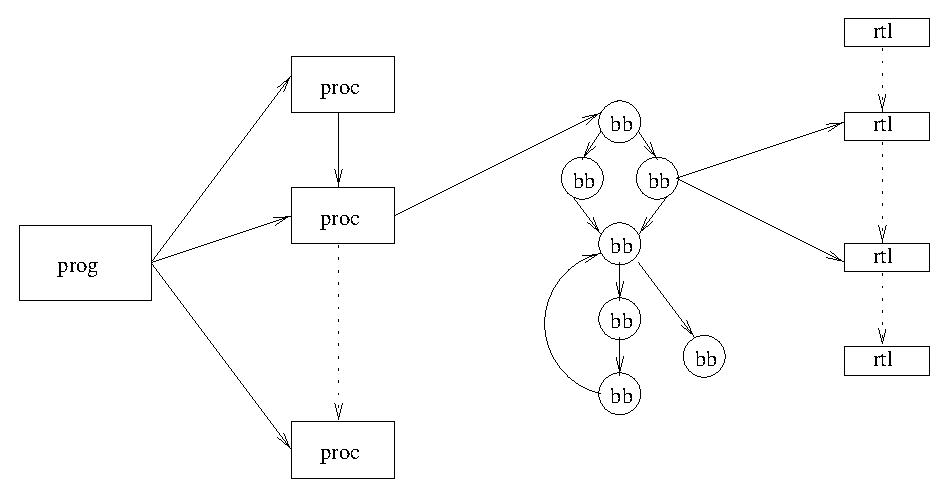
\includegraphics{figures/datastructs.eps}}
\centerfigend{fig-datastructs}{Data Structures to Represent a Binary Program}

We describe each of these parts of the intermediate representation
in reverse order, that is, starting from atomic data structures
and ending up with the program structure.



\section{Register Transfer Lists}
\label{sec-rtl}

{\small
\begin{flushright}
Design: Cristina, Mike; Documentation: Cristina, Doug, Mike;
 Implementation: Doug, David, Mike
\end{flushright} 
}

UQBT uses a simple, low-level register-transfer representation for the
effects of machine instructions.
A single instruction corresponds to a register-transfer list or RTL,
which in UQBT is a sequential composition of effects.
Each effect assigns an expression to a location.
All side effects are explicit at the top level;
expressions are evaluated without side effects, using purely
functional \emph{RTL operators}.
For example, the effects of the SPARC \texttt{call} instruction are
represented by the following RTL:

\begin{smallverbatim}
r[15] := %pc
%pc   := %npc
%npc  := r[15] + (4 * disp30)
\end{smallverbatim}
This sequence of effect puts the program counter~\texttt{\%pc} in
register~15, copies the ``next program counter''~\texttt{\%npc} into
the program counter, and puts the target address into~\texttt{\%npc}.
Because the target address is computed relative to the \emph{original}
program counter, the target-address computation uses register~15,
which holds the original value of~\texttt{\%pc}.
Because the SPARC uses delayed branches,  the target address
is placed into \texttt{\%npc}, not directly into \texttt{\%pc}.

Register transfer lists (RTLs) capture the semantic information 
of machine instructions by means of a series of \emph{effects} on a 
\emph{location}.
One register transfer is an assignment of an expression (i.e. an 
effect) to a location (i.e. a register or memory).  
There are no side effects, all effects are explicitly mentioned in 
the RTL.
The RTL environment assumes an infinite number of registers and
infinite memory space.  Memory is a sequence of bytes.  
{\it We will need specialized types of memory, such as memory for 
local variables, once the analysis has been formalized.   We
will do that then, so for now, there is only one type of memory. }

An `RTL language' is defined by a collection of locations and
operators.
UQBT uses an RTL language defined by taking the union of locations on
machines M$_S$ and M$_T$ and the union of the operators used in the
descriptions of machine M$_S$ and M$_T$.
The `machine~$X$ invariant' defines a sub-language of RTLs called
the $X$-RTLs; an RTL is an $X$-RTL if and only if it can be represented
as a single instruction on machine~$X$.

\uqbt 's \rtl\ implements the semantic information expressed in SSL
notation (SSL is described in Chapter~\ref{ch-ssl}).  

\subsection{Types}
\label{sec-rtltypes}
We define the following types to work with RTLs.  
(NOTE that these names should be in uppercase and perhaps shorter.
I've listed them as they appear in the rtl.h interface so that we don't
get confused -- when those are updated, these should be updated).
\begin{description}
\item[RTlist] a list of register transfers. Various analysis
    functions work on RTlists, such as GetControlTransfer().

\item[RTLInstDict] a dictionary of expanded instructions from the SSL
    file.

\item[RT] a register transfer is an assignment statement
    which has a variable (i.e. location) as the left-hand
    side and an expression (i.e. value) on the right-hand side. \\
    {\it We have considered introducing in the future a specialized
    RT which is a call, but at present that has not been decided
    upon.  We think it will be useful for analysis purposes. }

\item[RTAssgn] a subclass of class RT, representing an RT assignment
    (i.e. location := expression). One instruction may have zero
    (for NOP only) or more of these.

\item[RTFlagDef] a subclass of class RT, representing the definition
     of a flag function.

\item[RTFlagCall] a subclass of class RT, representing the call to a
    flag function.

\item[SemStr] a Semantic String, which is a prefix linearisation of an
    expression tree (see below).
    A SemStr can be used to represent a location, value, or subexpression.

    Expression operators are reproduced in Figure~\ref{fig-expOps2}.

% I'm not sure what this was meant to be about... probably some restriction
% on expressions which has long faded from the code. I keep it in comments
% in case it's not what I think it is. MVE
\begin{comment}
    {\it This may need to go elsewhere - Mike}
    An address expression is constrained to plus or minus offsets 
    from an address, hence the case \texttt{M[reg + reg * kte]} is not 
    supported directly; a subexpression needs to be computed into a 
    register and used as a register index in this case.

    These 3 options can be represented by 2: registers or constants.
    When an address expression is received, it is computed into 
    a register and that register is used to index into memory. 
    In this way we do not constrain address expressions (given that
    other machines may have more complicated addressing modes) 
    and create a simpler interface.
\end{comment}

\end{description}

\centerfigbegin
\begin{tabular}{|l|l|c|c|c|l|l|} \hline
Type of Operator & Id       &
\multicolumn{3}{c|}{Arguments}
& Symbol    & Meaning \\ \cline{3-5}
    &   & Int & Fix & Var & & \\
\hline
unary       & idNot         &0&0&1  & \verb!~!  & logical not \\
            & idNeg         &0&0&1  & 0-        & unary minus \\
\hline
binary      & idPlus        &0&0&2  & +         & addition \\
            & idMinus       &0&0&2  & -         & subtraction \\
            & idMult        &0&0&2  & *         & multiplication (unsigned)\\
            & idMults       &0&0&2  & *!        & multiplication (unsigned)\\
            & idDiv         &0&0&2  & /         & division (signed) \\
            & idDivs        &0&0&2  & /!        & division (signed) \\
            & idMod         &0&0&2  & \%        & modulus (unsigned) \\ 
            & idMods        &0&0&2  & \%!       & modulus (signed) \\ 
            & idBitAnd      &0&0&2  & \&        & (bitwise) and \\
%           & idBitAndNot   &0&0&2  & \&\~      & (bitwise) and-not \\
            & idBitOr       &0&0&2  & $|$       & (bitwise) or \\
%           & idOrNot       &0&0&2  & $|$\~     & (bitwise) or-not \\
            & idBitXor      &0&0&2  & \verb!^!  & xor \\
%           & idBitXorNot   &0&0&2  & \verb!^~! & xor-not \\
            & idShiftR      &0&0&2  & $>>$      & right-shift \\
            & idShiftL      &0&0&2  & $<<$      & left-shift \\
            & idShiftRA     &0&0&2  & $>>$A     & right-shift-arithmetic \\
            & idRotateL     &0&0&2  & rl        & rotate-left \\
            & idRotateR     &0&0&2  & rr        & rotate-right \\
            & idRotateLC    &0&0&2  & rlc       & rotate-left-through-carry \\
            & idRotateRC    &0&0&2  & rrc       & rotate-right-through-carry \\
\hline
ternary     & idTern        &0&0&3  & ?:        & c-style ternary \\
            & idAt          &0&0&3  & @         & bit extraction \\
\hline
logical     & idEquals      &0&0&2  & =         & equal \\
            & idNotEqual    &0&0&2  & \verb!~=! & not equal \\
            & idLess        &0&0&2  & $<$       & less than, signed \\
            & idGreater     &0&0&2  & $>$       & greater than, signed \\
            & idLessEq      &0&0&2  & $<=$      & less or equal to, signed \\
            & idGreaterEq   &0&0&2  & $>=$      & greater or equal to, signed \\
            & idLessUns     &0&0&2  & $<$u      & less than, unsigned \\
            & idGtrUns      &0&0&2  & $>$u      & greater than, unsigned \\
            & idLessEqUns   &0&0&2  & $<=$u     & less or equal to, unsigned \\
            & idGtrEqUns    &0&0&2  & $>=$u     & greater or equals, unsigned \\
            & idAnd         &0&0&2  & and       & and (of two expressions) \\
            & idOr          &0&0&2  & or        & or \\
\hline
operations  & idMemOf       &0&0&1  & m[...]    & memory of \\
            & idRegOf       &0&0&1  & r[...]    & register of \\
            & idAddrOf      &0&0&1  & a[...]    & address of (cancels m[]) \\
            & idVar         &1&0&0  & v\it{n}   & variable; replaces reg or mem \\
            & idParam       &0&1&0  & param`...'& parameter \\
            & idRparam      &0&1&0  & rparam`...'& register parameter \\
            & idExpand      &0&1&0  & expand`...'& expand (not for user) \\
            & idTemp        &0&1&0  & temp`...' & temporary register \\
            & idSize        &1&0&1  & size \it{n}& size cast \\
            & idDef         &0&1&0  & def `...' & definition; special for UQDBT \\
            & idIndex       &0&0&2  & [...]     & special for UQDBT \\
\hline
constants   & idIntConst    &1&0&0  & int \it{n}& integer constant \\
            & idFloatConst  &2&0&0  & float \it{f}& floating point constant \\
\hline
\end{tabular}
\centerfigend{fig-expOps2}{Expression Operators for RTL (cont over page)}

\centerfigbegin
\begin{tabular}{|l|l|c|c|c|l|l|} \hline
Type of Operator & Id       &
\multicolumn{3}{c|}{Arguments}
& Symbol    & Meaning \\ \cline{3-5}
    &   & Int & Fix & Var & & \\
\hline
type conversions& idSignExt &0&0&1  & !         & sign-extend (no sizes) \\
            & idTrunc       &2&0&1  & trunc(\it{exp, s1, s2})& truncate from s1 to s2 bits \\
            & idZfill       &2&0&1  & zfill(\it{exp, s1, s2})& zero fill from s1 to s2 bits \\
            & idSgnEx       &2&0&1  & sgnex(\it{exp, s1, s2})& sign extend from s1 to s2 bits \\
\hline
float conversions&idFsize   &2&0&1  & fsize(\it{exp, s1, s2})& float size convert from s1 to s2 \\
            & idItof        &2&0&1  & itof(\it{exp, s1, s2})& integer to float, s1 to s2 bits \\
            & idFtoi        &2&0&1  & ftoi(\it{exp, s1, s2})& float to integer, s1 to s2 bits \\
            & idFround      &2&0&1  & fround(\it{exp, s1, s2})& float round, s1 to s2 bits \\
\hline
\end{tabular}
\centerfigend{fig-expOps2a}{Expression Operators for RTL (cont from prev page)}

\subsection{Interface Functions to Create and Use RTLs}
All objects have constructor and destructor functions, as well
as functions to access elements of an object.  
Specialized analysis-related functions are explained in the
last subsection of this section---Functions for Analysis 
Purposes.  \\
{\it This style file doesn't number subsub sections,
how annoying! }


\subsubsection{Semantic String Class}
A semantic string object (SemStr) is a prefix linearisation of a tree
of RT components, such as constants, registers, memory, and various
expressions involving these. It is inplemented as a list of integers
(called items);
many of these integers are indices into a special table called the
Semantic Table. Entries in this table represent various things, such
as operators, special registers, parameters, and so on.

Here are a few examples: index 0 (the first entry) is called \texttt{idPlus},
and represents binary addition. Approximately index 75 is called
\texttt{idIntConst}, representing an integer (the actual integer is the next
integer in the string, following the {\tt idIntConst}).  So the expression
\texttt{2+2} is represented by the string ``{\tt 0 75 2 75 2}'' (read this
as ``plus int 2 int 2''). 

All the operators listed in Figure~\ref{fig-expOps2} are automatically
included in the table, and they are
machine independent. Special registers (e.g. the Next Program Counter register
({\tt \%npc}) and parameters (e.g. {\tt rs1} for the first source
register) are added
by the parser of the SSL file (see Chapter~\ref{ch-ssl}).
Let's consider a complete RTAssgn, conventionally written as

{\tt r[4] = m[1000] + 5}

This will be implemented as two semantic strings, one for the
location (left hand side) and one for the value (right hand side).
Each will be a list of integers, which might be

{\tt 34 75 4} ~~~and~~~ {\tt 0 38 75 1000 75 5}

and might print as

{\tt r[4]} ~~~and~~~   {\tt m[1000] + 5}  ~~~normally (the "int" is dropped
for brevity), or

{\tt r[ int 4]}  ~~~and~~~  {\tt + m[ int 1000 ] int 5}

if you choose to use the printPrefix() member function. This latter
representation is better for debugging problems with semantic strings,
though obviously it is less readable.

The first SemStr could be read as ``RegOf int 4''. The first integer, 34,
is an index into the semantic table, where among other information
there is the string ``r['' (for the SemStr print routine).
The enumerated constant ``idRegOf'' can be used in programs to
represent this index (see Figure~\ref{fig-expOps2} for a complete list
of these enumerated constants). The second integer,
75, is also an index into the semantic table, and says that the integer
following this index is to be taken as a literal integer. The third
integer, 4, represents itself. The second semantic string is a little
more complex. Its first index, 0, represents addition. The two arguments
to be added come next, but they are variable length. Immediately after
the 0 is 38, representing "memory of". The thing following the MemOf
could be any kind of expression; in this case it's ``int 1000'', but
it could have been say ``{\tt+ 500 500}'', or ``{\tt - r[ int 16 int 8}''.

Note that special registers (such as {\tt \%pc} or {\tt \%CF}) are
represented differently from general purpose registers. General purpose
registers are numbered, whereas special registers have their own
index into the semantic table (see Section~\ref{sec-semtable}).

A word on nomenclature: the word {\it parameter} is used to describe
a part of an instruction that will be {\it instantiated} with the
RTL function. For example, ``regorimm'' could be a parameter representing
a part of an instruction; actual values could be ``r[4]'' or ``4''.
The word {\it argument} is used here to mean those parts of a semantic
string that represent arguments (or operands) to the first index. For example,
if the first index is {\tt idMinus}, then there are two variable length
arguments to it, representing the minuend and the subtrahend respectively.
If the first index is idSize, there is one integer argument (the number
of bits in the size being cast to), and one variable length argument
(the expression being size cast).

Every semantic string has a type (e.g. unsigned integer 32 bits); the type is
represented by class Type (see Section~\ref{sec-class-type}). If not explicitly
specified, the semantic string is assigned the default type (which is signed
integer 32 bits). This type is preserved when semantic strings are copied,
subexpressions are made, and so on.

\begin{itemize}
\item   SemStr: $\emptyset$ \ra SemStr.
    Default constructor.

\item   SemStr: Kind \ra SemStr.
    Constructor that takes an expression kind. The kinds are only these:
    uORDINARY, eOPTABLE, and eCONDTABLE. Not for users.

\item   SemStr: SemStr \ra SemStr.
    Copy constructor.

\item   operator=: SemStr \ra SemStr.
    Assignment operator.

\item   SemStr: (Iterator1 x Iterator2) \ra SemStr.
    Constructor that takes a pair of iterators. Makes a copy of part
    of some other SemStr starting with the item referenced by iterator1
    up to but not including iterator2.

\item   SemStr: (int* x int* x Kind) \ra SemStr.
    Constructor that takes two pointers to an array of integers (pointer to
    first and pointer to last). Also takes kind, as above.

\item   getKind: SemStr \ra Kind.
    Gets the kind as above. Not for users.

\item   getType: SemStr \ra Type.
    Gets the type (as class Type) for the semantic string.

\item   isFloat: SemStr \ra BOOL.
    Note: deprecated. Returns true if the expression this semantic string
    represents is a floating point type.

\item   setType: (SemStr x Type) \ra $\emptyset$.
    Set the type for the expression that this semantic string represents.

\item   setTypes: (SemStr x SemStr) \ra $\emptyset$.
    Set the type for this semantic string to be the same as the type of the
    given semantic string.

\item   operator==: (SemStr x SemStr) \ra BOOL.
    Returns true if this SemStr is equal to the given SemStr. Type is taken
    into account in the comparison.

\item   operator\%=: (SemStr x SemStr) \ra BOOL.
    Same as above, except that type is \emph{not} taken into account.

\item   operator-=: (SemStr x SemStr) \ra BOOL.
    Same as the two above, except that only the sign element of the type is
    disregarded. Therefore, to return true, the expressions must match, and
    the size and broad type must match, but the ``signedness'' need not
    match.

\item   operator$<$: (SemStr x SemStr) \ra BOOL.
    Returns true if this SemStr is ``less than'' the given SemStr. Comparison
    is arbitrary, but establises a unique ordering of semantic strings. This
    function is often used implictly where there are maps of semantic strings.
    Type is included in the comparison.

\item   operator$<<$: (SemStr x SemStr) \ra BOOL
    Same as the above, except that ``signedness'' is not considered in the
    comparison.

\item   push: (SemStr x int) \ra $\emptyset$.
    Push the given integer to the end of the semantic string. It is up to
    the user to make sure that the semantic string is valid.

\item   prep: (SemStr x int) \ra $\emptyset$.
    Prepend the given integer to the front of the semantic string. It is
    up to the user to make sure that the semantic string is valid.

\item   pushSS: (SemStr x SemStr) \ra $\emptyset$.
    Push a copy of the given semantic string to the end of this string

\item   pushArr: (SemStr x int x int*) \ra $\emptyset$.
    Push the given number of integers from the given array of integers to
    the end of the string.

\item   pop: $\emptyset$ \ra int.
    Remove the last integer from the list, and return it.

\item   popFirst: $\emptyset$ \ra int.
    Remove the first integer from the list, and return it.

\item   clear: $\emptyset$ \ra $\emptyset$.
    Set this semantic string to be empty (no elements in the list).

\item   isSpRegEqual: (SemStr x int) \ra BOOL.
    Returns true if this semantic string matches the special register
    whose index is given. Not for most users.

\item   isSpRegCont: (SemStr x int) \ra BOOL.
    Returns true if this semantic string contains the special register
    whose index is given. Not for most users.

\item   isNumRegEqual: (SemStr x int) \ra BOOL.
    Returns true if this semantic string matches the register
    whose number is given. Not for most users.

\item   isNumRegCont: (SemStr x int) \ra BOOL.
    Returns true if this semantic string contains the register
    whose number is given. Not for most users.

\item   isArrayEqual: (SemStr x Array of int) \ra BOOL.
    Returns true if the elements of this semantic string match the
    elements of the given array of integers. Can be used to test for
    specific semantic strings, e.g. ``\%pc = \%npc''.

\item   getFirstIdx: SemStr \ra int.
    Returns the first item of this semantic string. Note that this really
    should be called getFirstItem, since the integer returned may not actually
    be an index (it could be an integer constant, or even half of a floating
    point constant).

\item   getSecondIdx: SemStr \ra int.
    Returns the second item of this semantic string. Usually used where
    the first index is known to contain one integer or fixed argument
    (e.g. the first index is idIntConst or idSize).

\item   getThirdIdx: SemStr \ra int.
    Returns the third item of this semantic string.

\item   getSubExpr: (SemStr x int) \ra SemStr*.
    Returns a pointer to a new semantic string, which is composed of
    the given subexpression. Passing zero returns the first argument
    to this expression, one returns the second, and so on.
    {\bf Note:} This member function only works with variable arguments.
    Use GetSecondIdx to access an integer or fixed argument.

\item   getSubExpr: (SemStr x int x SemStr) \ra SemStr.
    As above, but also stores the result in the reference (last) parameter.
    This ensures that the caller will automatically delete the semantic string
    when it goes out of scope.

\item   getIndex: (SemStr x int) \ra int.
    Get the {\it i}th item (where {\it i} is given).

\item   getLastIndex: SemStr \ra int.
    Get the last item of the list of integers in this semantic string.

    The next group of member functions concern searching for a subexpression
    withing this semantic string. An item of -1 in a semantic string is treated
    as a ``wildcard''.
    Formally, a search expression (S) will match a subexpression (E) if:

    length(S) $<=$ length(E) and for each position, p, in S the following holds:

    S[p] == -1 $||$ S[p] == E[p]

    Example: if {\it this} is \{0,\{3,78\},\{43,6,14\}\},
    it can be searched with the following subexpressions, and will return true:

\begin{tabular}{|l|l|} \hline
    Search & Result \\
\hline
    \{\{3,78\}\} & \{\{3,78\}\} \\
    \{\{0,*,*,\{43\}\}\} & \tt\{\{0,\{3,78\},\{43,6,14\}\}\} \\
\hline
\end{tabular}

\item   search: (SemStr x SemStr x SemStr x BOOL) \ra BOOL.
    Searches this semantic string for the given subexpression (first parameter
    after {\it this}). If found, the matching string is copied to the reference
    (last SemStr) parameter. The return value is whether a match was found.
    If the optional boolean is set, the search is type
    sensitive (i.e. the types have to match, as well as the expressions). This
    boolean defaults to false (i.e. the search defaults to case insensitive).

\item   searchAll: (SemStr x SemStr x list\{SemStr*\} x BOOL) \ra BOOL.
    Searches this semantic string for {\it all} occurrences of the given
    subexpression (first parameter after {\it this}). For each match, the
    matching string is appended to the list of pointers to semantic strings.
    The return value is whether any match was found.
    If the optional boolean is set, the search is type
    sensitive (i.e. the types have to match, as well as the expressions). This
    boolean defaults to false (i.e. the search defaults to case insensitive).

\item   searchReplace: (SemStr x SemStr x SemStr x BOOL) \ra BOOL.
    Searches this semantic string for the given subexpression (first parameter
    after {\it this}). If found, the matching string is replaced by the
    reference (last SemStr) parameter. The return value is whether a match was
    found.
    If the optional boolean is set, the search is type
    sensitive (i.e. the types have to match, as well as the expressions). This
    boolean defaults to false (i.e. the search defaults to case insensitive).

\item   searchReplaceAll: (SemStr x SemStr x SemStr x BOOL) \ra BOOL.
    Searches this semantic string for {\it all} occurrences of the given
    subexpression (first parameter after {\it this}). For each match, the
    matching string is replaced by the given string (last SemStr parameter).
    The return value is whether any replacement was made.
    If the optional boolean is set, the search is type
    sensitive (i.e. the types have to match, as well as the expressions). This
    boolean defaults to false (i.e. the search defaults to case insensitive).

\item   substReg: (SemStr x int x SemStr) \ra BOOL.
    Substitute all occurrences of the given numbered register with the given
    semantic string. Returns true if any match found.
 
\item   substSpcl: (SemStr x int x SemStr) \ra BOOL.
    Substitute all occurrences of the given special register (index is given)
    with the given semantic string.

\item   substIndex: (SemStr x int x int) \ra $\emptyset$
    Replace the item at the given index with the given integer. For example,
    substIndex(0, 77) will replace the first item in the list with 77.
 
\item   smartCompare: (SemStr x SemStr x BOOL x list\{int\}) \ra BOOL.
    This function is not complete. Do not use.

\item   findEndSubExpr(SemStr x iterator) \ra iterator.
    Given an iterator into this semantic string, step forward towards the end
    of this string until the end of the subexpression headed by the given
    iterator is found. Returns an iterator that is just past the end of that
    subexpression. For example, if given (3+4)*(5+6) (internally
    * + int 3 int 4 + int 5 int 6), with an iterator pointing to the first
    plus, returns an iterator to the second plus (just past the (3+4)
    subexpression).
    There are actually two functions with the same name; one takes and
    returns a const iterator, and one takes and returns a non-const iterator.

\item   simplify: SemStr \ra $\emptyset$
    Simplify this expression using constant folding and the like, and also
    cannonicalising the expression by placing integer constants on the
    right if possible (so 2+a is replaced by a+2). a + -2 is replaced by a-2.
    a $<<$ k is changed to a * K where K=2**k.

\item   findSubExpr: (SemStr x int x int* x int) \ra BOOL.
    Search this semantic string for the expression (given by the given number
    of integers in the given array of integers). Returns true if found. If
    found and there were wildcards in the array, the item matched by the last
    wildcard is written to the reference (last) parameter.

\item   sprint: SemStr \ra string.
    Prints a representation of this semantic string to a string, which
    is returned. This is a conventional (infix) representation, and
    so it somewhat removed from the actual (prefix) implementation.
    Some effort is made to pretty the result, e.g. r[ int 4] is
    displayed as r[4].
    When exact knowledge of the format of the string is required, use
    sprintPrefix below.

\item   print: (SemStr x ostream) \ra $\emptyset$.
    Prints a representation of the semantic string to the given stream,
    or to cout if none is given. It is equivalent to printing the string
    returned by sprint to the given stream.

\item   sprintPrefix: SemStr \ra string.
    Prints a representation of this semantic string to a string, which
    is returned. The format is strongly tied to the internal (prefix)
    representation of the semantic string, so it is harder to read than
    the result from sprint, but may be more useful for debugging.

\item   printPrefix: (SemStr x ostream) \ra $\emptyset$.
    Prints a representation of the semantic string to the given stream,
    or to cout if none is given. It is equivalent to printing the string
    returned by sprintPrefix to the given stream.

\item   len: SemStr \ra int.
    Returns the number of items in this semantic string.

\item   instantiate: (SemStr x list\{int\} x vector\{char*\} x RMAP) \ra BOOL.
    Replace all occurrences of formal instruction parameters (e.g. rs1) with
    actual expressions (e.g. r[12]). The last parameter is an object
    representing the register map. Not for users.

\end {itemize}

\subsubsection{Semantic Table Class}
\label{sec-semtable}

Semantic Strings (class SemStr) are mainly indices into a special
object of class SemTable, the semantic table. This is a global
object, accessable as {\tt theSemTable} as long as you
{\tt \#include "ss.h"}. Most of the time, the user need not be
concerned with the semantic table, but there are a few important
exceptions.

One of these is when dealing with special registers. These registers
are not accessed like general purpose registers (so called {\it numbered}
registers), but have their own entries in the semantic table. When
special registers are referenced in the SSL file (see Chapter~\ref{ch-ssl}),
they are placed into
the semantic table by the parser. The index of a particular special
register is not fixed (most of them are machine specific), so there is no
enumerated constant like {\tt idPlus} that can be used for a special
register. At present, the way to find an appropriate index is to use
the FindRegIndex member function.

\begin{itemize}
\item   findRegIndex: (SemTable x string) \ra int.
    Given the semantic table and a string representing the name of the
    special register (including the {\tt \%}), returns an integer index
    for the appropriate semantic table item. This single index
    represents the special register in semantic strings (compared with
    three integers for a numbered register).

\item   findOpIndex: (SemTable x char*) \ra int.
    Given a C string representing the operator (e.g. {\tt \verb!"&~"!}),
    returns the index representing the operator. This operator can be
    used to build expressions, etc. Note that this function is not
    efficient (at present, it uses a linear search), so it should not
    be used where the operator is known (in this case, {\tt idBitAndNot});
    use it where the operator could be one of a number of values, and
    only the string representation is known. (For example, the SSL
    parser uses this function when parsing SSL expressions).

\end{itemize}

\subsubsection{Type Class}
\label{sec-class-type}
Types inside Semantic Strings and elsewhere are represented by class Type.
A Type has three components: the broad type, sign, and size. The broad type
is given in terms of this enumerated type:

\begin{verbatim}
enum LOC_TYPE {
    VOID = 0,               // void (for return type only)
    INTEGER,                // integer (any size and signedness)
    FLOAT,                  // a floating point (any size)
    DATA_ADDRESS,           // a pointer to some data (e.g. char*, struct*,
                            // float* etc)
    FUNC_ADDRESS,           // a pointer to a function
    VARARGS,                // variable arguments from here on, i.e. "..."
    UNKNOWN
};
\end{verbatim}

A particular type is given by either a tuple (e.g. (INTEGER, unsigned, 32 bits))
or a couple (e.g. (FLOAT, 64 bits); the sign is irrelevant for a float, but
defaults to signed).

\begin{itemize}
\item   Type: $\emptyset$ \ra Type.
    Default constructor. Returns the default type, which is 32 bit signed
    integer.

\item   Type: (LOC\_TYPE x int x BOOL) \ra Type.
    Constructor, with type given as a LOC\_TYPE (see abvove), size in bits,
    and if the LOC\_TYPE is integer, a BOOL for sign (TRUE = signed).

\item   operator==: (Type x Type) \ra BOOL.
    Equality operator. Sign is considered in the comparison, so the types must
    match in all respects for this function to return TRUE.

\item   operator-=: (Type x Type) \ra BOOL.
    Equality operator. Sign is {\it not} considered, so for this function to
    return true, the broad types and size must match, but the sign need not.

\item   operator$<$: (Type x Type) \ra BOOL.
    Less than operator. Sign is considered in the comparison.
    This function establishes an arbitrary ordering among all types.

\item   operator$<<$: (Type x Type) \ra BOOL.
    Less than operator. Sign is {\it not} considered in the comparison.
    This function establishes an arbitrary ordering among all types.

\item   getSize: Type \ra int.
    Returns the size (in bits) component of the Type.

\item   getType: Type \ra LOC\_TYPE.
    Returns the Type component of the Type, as a LOC\_TYPE.

\item   getSize: Type \ra BOOL.
    Returns the sign component of the Type; TRUE if signed.

\item   setSize: (Type x int) \ra $\emptyset$.
    Sets the size (in bits) component of this Type.

\item   setType: (Type x LOC\_TYPE) \ra $\emptyset$.
    Sets the Type component of this Type, given a LOC\_TYPE.

\item   setSize: (Type x BOOL) \ra $\emptyset$.
    Sets the sign component of this Type; TRUE if signed.

\item   getCtype: Type \ra CHAR*.
    Returns a C-style null terminated string representing the C language
    equivalent of the type. For example, if the type is (integer, unsigned, 16)
    the returned string would be ``unsigned short''.

\end{itemize}


\subsubsection{Register Transfer Assignment Class}
A register transfer assignment (RTAssgn) object is an assignment of an
expression
to a location.  A register transfer object also has size information
to determine the number of bits of information transferred from
the expression to the location.

\begin{itemize}
\item  updateLHS: (RTAssgn x Location) \ra RT.
    Given an RT object and a location, the location
    information gets updated in the object.

\item  updateRHS: (RTAssgn x Expr) \ra RT.
    Given an RT object and an expression, the expression
    information gets updated in the object.

\item  updateSize: (RTAssgn x BYTE) \ra RT.
    Given an RT object and a size in bits, the size of the
    transfer information gets updated in the object.

\item  getLHS: RTAssgn \ra SemStr*.
    Given an RTAssgn object, returns a pointer to the semantic string
    representing the location of the assignment.

\item  getRHS: RTAssgn \ra SemStr*.
    Given an RTAssgn object, returns a pointer to the semantic string
    representing the expression of the assignment.

\item  getSize: RTAssgn \ra BYTE.
    Given an RT object, returns the size in bits of the transfer
    of information.
\end{itemize}


\subsubsection{Register Transfer List Object}
A register transfer list (RTlist) is a list of register transfer 
objects.  However, greater functionality is provided for this 
object for analysis purposes; those functions are described in the 
next section.
For traversal purposes, an RTlist keeps track of the `current'
register transfer being traversed (by default, the first one
in the list).

\begin{itemize}
\item RTlist: $\emptyset$ \ra RTlist.
    Constructor function which returns an empty object of type RTlist.

\item RTlist: (RTlist x RTlist) \ra RTlist.
    Copy constructor: given a source and destination RTlist 
    objects, copies the first one onto the second one.

\item insertRT: (RTlist x RT) \ra RTlist.
    Given an RTlist object and a register transfer, inserts the
    register transfer at the end of the list.

\item updateRT: (RTlist x RT x int) \ra RTlist.
    Given an RTlist object, a register transfer and an index position into
    a list, updates the indexed register transfer in the list
    with the new one (if possible), otherwise it does not modify
    the RTlist object.
\end{itemize}


\subsubsection{Functions for Analysis Purposes}
The following functions are required for analysis purposes and
are described per relevant object.
More functions will be added as we see fit.


\paragraph{Register Transfer Assignment Class}
Functions that allow users to know which registers are defined
and used in the register transfer.  Note that this information
is implicitly stored in the LHS and RHS fields of an 
RTAssgn object.

\begin{itemize}
\item  isSpRegDefined: (RTAssgn x int) \ra BOOL.
    Given a register transfer assignment object and an index representing
    a special register, returns 
    whether the register is defined in the assignment or not.

\item  isNumRegDefined: (RTAssgn x int) \ra BOOL.
    Given a register transfer assignment object and the number of a
    numbered register, returns whether that register was defined
    in the register transfer or not.

\item  isSpRegUsed: (RTAssgn x int) \ra BOOL.
    Given a register transfer assignment object and an index representing
    a special register, returns whether
    that register was used by the object or not.

\item  isNumRegUsed: (RTAssgn x int) \ra BOOL.
    Similar to IsRegUsed() but for a numbered register.

\item  numRegUse: RTAssgn \ra int.
    Given a register transfer object, returns the number of registers
    used by that transfer. \\
    {\it Not implemented at present. A similar function that returns a list of registers used may
    be useful. }

\item  numRegDef: RTAssgn \ra int.
    Given a register transfer object, returns the number of registers
    that were defined by that transfer. \\
    {\it Not implemented at present. A similar function that returns a list of registers defined may
    be useful. }
\end{itemize}


\paragraph{Register Transfer List Object} 
The RTlist object \emph{will} provide in the \emph{future} 
functions that allow us to quickly decide what type of 
instructions we are dealing with.  The following are two
such functions which are not currently implemented:

\begin{itemize}
\item RTL: (STRING x ADDRESS x ...) \ra RTlist.
    This function returns an instance of a register transfer
    list for a particular machine instruction.  The name
    of the instruction is a named used in the SSL specification,
    these names are normally the same names used in SLED
    specifications.   The given native address is the program counter's
    address and is stored for usage when building a control
    flow graph of the procedure (see Section~\ref{sec-cfg}). \\ 
    The function returns an instance of an RTlist by reading
    the template file generated by SRD (refer to Section~\ref{sec-srd},
    Chapter~\ref{ch-ssl}).  \\

\item getBBSuccAddr: (RTlist x int) \ra ADDRESS.
    Given an RTlist object and an index position, returns the 
    address associated with that out-edge (if any) or Nil 
    otherwise.  \\
    This function is useful to construct a control flow graph,
    see example in Section~\ref{sec-cfg-eg}. 

\item getBBProcAddr: RTlist \ra ADDRESS.
    Given a call register transfer list, returns the target procedure 
    call address (if any) or Nil otherwise. \\
    This function is useful to construct a control flow graph,
    see example in Section~\ref{sec-cfg-eg}.

\item getNumRT: RTlist \ra int.
    Given an RTlist, returns the number of elements (RTs) in
    the list.

\item getRT: (RTlist x int) \ra RT.
    Given an RTlist object and an index into the list, returns
    the corresponding register transfer (if it exists) or 
    Nil.
    Elements in a list are indexed from one.

\item nextRT: RTlist \ra RT.
    Given an RTlist object, returns the next RT in the list (if any)
    or Nil (if at the end of the list).  The `current' index is
    updated to point to the next element in the list. 

\item isControlTransfer: RTlist \ra CTTYPE.
    Given an RTlist object, checks if the set of register 
    transfers are equivalent to a control transfer instruction,
    if so, returns the type of control transfer instruction 
    (one of ONEWAY, TWOWAY, NWAY, CALL, or FALL), otherwise
    returns NONE.  
    A control transfer instruction is one that explicitly 
    modifies the value of the program counter register.
\end{itemize}



\subsection{Usage of this Interface}
\label{sec-usageRTL}
A user can integrate RTL into a NJMC matching statement in
the following way: once an instruction has been decoded 
by matching one of the arms of the \texttt{match} statement, 
an instance of the matched instruction can be obtained in 
RTL form by passing the (unique) name of the instruction to
the RTL dictionary, along with the values of the other parts
of the instruction.  The RTL system will return an instance
of an entry in the dictionary. 
At present, the RTL instance function expects to receive 
the native address of the instruction being decoded, its name 
(i.e. key), and its arguments in string form.  The native 
address is required later on, for the purposes of constructing
a control flow graph of the program (see Section~\ref{sec-cfg}).

The following sample code illustrates the usage of this interface
with a SPARC matching statement.
The function \texttt{decode\_instr} implements a matching statement
which decodes the machine instruction pointed to by the \texttt{pc}
variable.  If the \texttt{alu} arm is matched, the \texttt{name} 
variable will hold the name of the arithmetic-logical instruction
matched.  The \texttt{RTLDisc.RTL} function is called with the
string values for the other parts of the arithmetic-logical 
instruction: the first register operand (\texttt{rs1}), the 
second register or immediate operand (matched in the \texttt{dis\_roi}
function), and the destination register \texttt{rd}).  Macros
are used (\texttt{RS1}, \texttt{ROI} and \texttt{RD}) to make
the translation from integer to strings depending on the context.
In the case of branch and call instructions, the target address passed
to the RTL dictionary is the \emph{raw} offset address given in the
instruction, rather than the relocated one; hence the need for the
equation provided to restore this value.  Alternatively, the 
core SLED spec for SPARC could be modified so that it does not 
relocate addresses automatically---this has not been done at 
present for consistency with disassemblers.

{\small
\begin{verbatim}
#define RD   (rd_names[rd])
#define RS1  (rs1_names[rs1])
#define RS2  (rs2_names[rs2])
#define ROI  (dis_roi(roi))

char *dis_roi(ADDRESS lc) {
  static char buf[512];
  match lc to
  | imode(i)   => sprintf(buf, "%d", i); return buf;
  | rmode(rs2) => return RS2;
  endmatch
}

void decode_instr (ADDRESS pc, ADDRESS uNativeAddr, RTLInstDict RTLDict, RTlist &rtl)
{
    match pc to
    | ...
    | alu (rs1, roi, rd) [name] => 
            rtl = RTLDict.RTL (uNativeAddr, name, RS1, ROI, RD);
    | branch^a (tgt, a) [name] => 
            sprintf(anulled, "%d", a);      // 1 if anulled
            rtl = RTLDict.RTL (uNativeAddr, name, numToStr((tgt-pc)>>2), anulled);
    | call_ (tgt) [name] => 
            rtl = RTLDict.RTL (uNativeAddr, name, numToStr((tgt-pc)>>2)); 
    | ...
    endmatch
\end{verbatim}  
}

This type of code (the whole matching statement file) can
obviously be mostly generated automatically, but at this stage we
either generate a decoder usingthe NJMC toolkit and modify that
code, or write it manually.


\section{Control Flow Graphs}
\label{sec-cfg}

{\small
\begin{flushright}
Design: Cristina; Documentation: Cristina; Implementation: Mike, Cristina
\end{flushright} 
}

A control flow graph (CFG) is a directed graph that represents the flow of 
control of a program, thus, it only represents the flow of instructions 
(code) of the program and excludes data information.
The nodes of a CFG represent basic blocks of the program, and the edges 
represent the flow of control between nodes.  More formally,

\begin{definition} \cite{Aho86}
\label{def-bb}
A {\bf basic block} is a sequence of consecutive statements in which
flow of control enters at the beginning and leaves at the end without
halt or possibility of branching except at the end.   
\end{definition}


\begin{definition}
\label{def-cfg}
A {\bf control flow graph} $G = (N,E,h)$ for a program $P$ is a connected,
directed graph, that satisfies the following conditions:
\begin{itemize}
\item $h$ is the unique entry node to the graph, 
\item $\forall \, n \in N, n$ represents a basic blocks of $P$, and 
\item $\forall \, e = (n_{i},n_{j}) \in E, e$ represents flow of control from
basic block $n_{i}$ to basic block $n_{j}$, and $n_{i}, n_{j} \in N$.
\end{itemize}
\end{definition}


\subsection{Types of Basic Blocks}
For the purposes of CFG construction, basic blocks are
classified into different types, according to the {\em last} instruction in 
the basic block.  Given that the instructions in the basic block
represent a sequential list of instructions (that would be executed
in that order), machine dependencies on the flow of control such as 
SPARC's delayed instructions cannot appear in the graph; they need
to be abstracted away into a machine-independent form.

Ideally, only 6 types of basic blocks are available.  However, 
during static decoding of a binary executable, it is not always
possible to determine the target branches of indirect and indexed
transfers of control.  In these cases, we make use of a node called
{\em nowhere} as the node does not lead to anywhere.  This node
will be analysed at runtime.  
The basic block types are: 

\begin{description}
\item [one-way] the last instruction in the basic block is an
unconditional jump to a known target location, hence, the block has one 
out-edge.

\item [two-way] the last instruction is a conditional jump to a 
known target location, thus, the block has two out-edges.

\item [n-way] the last instruction is an indexed/indirect jump to
known target locations.  The $n$ branches located in the index table become 
the $n$ out-edges of this node.

\item [call] the last instruction is a call to a procedure.
There are two out-edges from this block: one to the instruction following
the procedure call, and the other to the procedure that is called.
Throughout analyses, the called procedure is normally not followed,
unless interprocedural analysis is required.

\item [return] the last instruction is a procedure return instruction.
There are no out-edges from this basic block.

\item [fall] the next instruction is the target address of a
branch instruction (i.e. the next instruction has a label).  This node
is seen as a node that {\it falls through} the next one, thus, there is
only one out-edge.

\item [nowhere] the last instruction is an indexed or indirect jump
or call to an unknown target location.  This node has no out-edges. 
\end{description}


\subsection{Abstractions}
Based on definitions~\ref{def-bb} and \ref{def-cfg}, we define two 
abstractions to work with control flow graphs.

\begin{description}
\item [BB] is a basic block.  A BB holds information about the
    RTL instructions that form part of that basic block, as 
    well as successors of the basic block.

\item [CFG] is a control flow graph.  A CFG is a reference to 
    the header of the graph, i.e. a BB, and stores extra information
    like the state of the graph (see next section).
    Extra functionality is provided for a CFG which is not 
    provided for a BB, as seen in Section~\ref{sec-ir-cfg}.
\end{description}


\subsection{Steps in Constructing a CFG}
Machine instructions that modify the flow of control of a program 
have two types of references to the target address: via a machine-dependent
(physical) address, or via an offset into the stream of machine
instructions for the program.  Offsets resolve to physical 
addresses too.   
There are three main steps in the construction of the CFG:
\begin{enumerate}
\item Create a machine-dependent CFG by building BBs of instructions
    that contain native addressess for transfers of control.
\item Transform the machine-dependent CFG into a machine-independent
    CFG by transforming address references into edges (references
    to basic blocks).
\item Optimize the machine-independent CFG to remove extraneous 
    basic blocks introduced by limitations in the machine 
    instruction set (e.g. a jump to a jump), hence reducing the 
    number of nodes and edges of the graph. 
\end{enumerate} 

We will refer to the machine-independent CFG as a {\em well-formed} CFG
or \wfCFG.  This graph is the one used for analysis purposes. 


\subsection{Interface Functions to Construct Basic Blocks}
\label{sec-ir-bb}
Basic blocks have limited functionality: they can be 
constructed, and machine-dependent (i.e. host address) out-edges 
can be added to them. 

\begin{itemize}
\item BasicBlock: $\emptyset$ \ra BB.
    Constructor for a basic block.

\item addOutEdge: (BB x ADDRESS) \ra BOOL.  
    Adds the address as an out-edge in the given basic block. 
    The mapping between addresses and basic blocks is done when 
    the graph is well-formed.
    Returns true if successful.

\item addInterProcOutEdge (BB x ADDRESS) \ra BOOL.
    Adds an interprocedural out-edge to the basic block pBB that
    represents this address.  The mapping between addresses and
    basic blocks is done when the graph is well-formed.
    Returns true if successful.

\item addProcOutEdge: (BB x ADDRESS) \ra BOOL.
    Given a CALL basic block and an address of a procedure (i.e. the
    target address of a call instruction), stores the information
    in the basic block. 
    \emph{This function is not yet implemented.}
\end{itemize}


\subsection{Interface Functions to Construct a CFG}
\label{sec-ir-cfg}
Control flow graphs are composed of machine-dependent basic block nodes 
initially, and can then be transformed to machine-independent nodes
which are used for analysis purposes.  This latter graph is referred
to as a well-formed graph. 
A doubly-linked graph (i.e one that has in- and out-edges) can only be 
built once the graph is well-formed.
Further, a well-formed graph can be optimized to remove redundant edges 
and nodes (e.g. jumps to jumps).
The following functionality is provided by the interface:

\begin{itemize}
\item Cfg: $\emptyset$ \ra Cfg.
    Constructor function for a CFG. The CFG is constructed empty, and
    has BBs added as required.

\item newBB: (CFG x RTL x RTL x BBTYPE x int x ADDRESS) \ra BB.  
    Allocates memory for a new basic block node, initializes it to 
    references to the first and last rtl's, its type, and allocates 
    enough space to hold the out-edges (the number of which is 
    given as a parameter).  
    The native address associated with the start of the BB is given;
    this address must be the same one used with AddOutEdge().
    A reference to the newly created basic block is returned.
    If there is not enough memory, an exception will be raised.
    \emph{Mike: what did we decide in the end for these cases?}

\item label: (CFG x ADDRESS) \ra BOOL.
    Checks whether the given native address is a label (explicit or 
    non-explicit) or not.  Explicit labels are addresses that have already 
    been tagged as being labels due to transfers of control to that 
    address.  Non explicit labels are those that belong to basic blocks 
    that have already been constructed (i.e. have previously been 
    parsed) and now need to be made explicit labels.  In the case of 
    non explicit labels, the basic block is split into two and types 
    and edges are adjusted accordingly.
    Returns true if the native address is that of an explicit or a non 
    explicit label, false otherwise. 

\item isLabel: (CFG x ADDRESS) \ra BOOL.
    Checks if the native address is a label or not in the current 
    control flow graph. 
    If not, the address is not added to the map of Lables to BBs.
    \emph{Mike: what does the last sentence mean?  i.e. every time
    an IsLabel() command is emmited, new labels are created??}

\item wellFormCFG: CFG \ra BOOL.  
    Transforms a machine-dependent CFG into a well-formed CFG (\wfCFG) 
    (i.e. a machine-independent one), by converting address references 
    of out-edges into references to basic blocks, and procedure
    address references into references to procedure structures 
    (the procedure structure is defined in Section~\ref{sec-ir-proc}).  
    Returns TRUE if successful.

\item isWellFormed: CFG \ra BOOL.
    Returns whether the graph is well-formed or not.

\item addInEdges: CFG \ra BOOL.  
    Given a \wfCFG, annotates each basic block with its in-edges 
    information.  Returns TRUE if successful.

\item compressCFG: CFG \ra BOOL.  
    Given a \wfCFG, optimizations are performed on the graph to reduce 
    the number of basic blocks and edges (if possible).  Returns
    TRUE if successful (whether or not the graph was compressed).
    The optimizations performed are: removal of branch
    chains (i.e. jumps to jump), removal of redundant jumps (i.e. jump
    to the next instruction), merge basic blocks where possible, and
    remove redundant basic blocks created by the previous optimizations.
\end{itemize}


\subsection{Interface Functions for Analysis Purposes}
Analysis functions are available to graphs of any kind; well-formed
or not.
In order to traverse a graph, a numbering scheme needs to be used
to uniquely identify the nodes in the graph in some fashion.  
For display purposes, the graph itself needs to be stored in a 
notation amenable for display, such as that provided by the Dotty 
interface. 

\begin{itemize}
\item numberCFG: CFG \ra BOOL.  
    Given a \wfCFG, each node in the graph is annotated with a unique 
    integer identifier.
    The method used at present is depth-first traversal, numbering
    nodes during the first visit to the node.
    We may change this numbering method later on.  
    Returns TRUE if successful.

\item writeDotFile: (CFG x STRING x int) \ra BOOL.  
    Given a \wfCFG\ and the name of an opened dotty (.dot) file,
    writes the information relating the control flow graph with
    node IDs offset by an integer value.  This property is used
    to give unique ID numbers to all nodes in a dotty file (a 
    requirement of the dotty interface).
    Returns TRUE if successful.
\end{itemize}


\subsection{Usage of this Interface}
\label{sec-cfg-eg}
A user may construct a control flow graph after having decoded  
the machine instructions and obtained their semantical 
RTL representation (see Section~\ref{sec-usageRTL}).  
Higher order instructions prevent us from creation of the graph 
at decoding time, due to the dependency of such instructions 
on an undecoded instruction.
\emph{However, note though that our current implementation 
creates basic blocks while decoding machine instructions; 
this gives us an approximation of the final graph but not 
a correct graph necessarily.  Analysis to remove higher order instructions
is missing at present, but is underway (in paper at least) -- cc,
27 May 98.}

The process of creating a \wfCFG\ is divided into two steps:
creating the basic blocks and creating the machine-independent
graph.  The former step can be done during the decoding of
machine instructions, as per the following code illustrates.
The function \texttt{followControl} drives the decoding of 
machine instructions by traversing paths in the program. 
While the code along one path has not been traversed, the 
function decodes one instructions (\texttt{decode\_instr}) and
checks if it is a control transfer instruction.  If so, based
on the type of the instruction, the type of the new basic
block is determined.  For example, if the parsed instruction
was an unconditional branch, then a one-way node is created,
with references to the first (\texttt{hdr}) and the last (\texttt{end})
rtls, and the target address of the jump. 
Once a node has been created, the target address is traversed 
recursively if it has not been traversed yet.  This is easily checked by 
determining if the target address is a label in the current 
graph or in another graph (as it may be an interprocedural branch).
The address for the next instruction to decode is determined, 
as well as the end of the section is checked.  The new target 
address is also checked for having been traversed---if it has, this
means that a fall-through node needs to be created rather than
decoding the same instructions twice.

{\small
\begin{verbatim}
// followControl()
// Precondition: the passed uNativeAddr is within the boundaries of
// the code section being decoded (i.e. uNativeAddr < upperNativeAddr).
// Precondition 2: the passed uNativeAddr is not an explicit label.
//
void followControl (ADDRESS uHostAddr, ADDRESS uNativeAddr,
                    ADDRESS upperNativeAddr, RTLInstDict RTLDict, LRTL &rtls,
                    Cfg &cfg)
{ BOOL done;
  INSTYPE type;
  RTL_CIT hdr, end;
  PBB pBB;

    while (! done)
    {
        // decode the inst at uNativeAddr (pointed to by uHostAddr)
        decode_instr (uHostAddr, uNativeAddr, buffer, RTLDict, rtl);

        // traverse paths based on flow of control
        if (rtl.getControlTransfer (type))
           switch (type)   {
           case I_UNCOND:
               end = --rtls.end();
               pBB = cfg.newBB (hdr, end, ONEWAY, 1, (*hdr).getAddress());
 
               // calculate new addresses and add to BB edge
               newNativeAddr = rtl.GetOutAddr (0);
               newHostAddr = uHostAddr + (newNativeAddr - uNativeAddr);
               pBB->addOutEdge (newNativeAddr);
 
               // follow target address if it hasn't been parsed yet
               if ((cfg.Label (newNativeAddr) == false) &&
                   (prog.isProcLabel (newNativeAddr) == false) &&
                   (newNativeAddr < upperNativeAddr))
                   followControl (newHostAddr, newNativeAddr, upperNativeAddr, 
                                  RTLDict, rtls, cfg);
               done = true;            // no more paths along this branch
               break;

           // ...

           case I_RET:
               end = --rtls.end();
               pBB = cfg.newBB (hdr, end, RET, 0, (*hdr).getAddress());
               done = true;    // path ends here, flag so
               break;
           } // switch

        // calculate address of next instruction
        // check if the end of the section is reached (i.e. out of bounds)
 
        // check if next address to decode has already been parsed,
        // if so, add a fall-through node when needed.
        if (cfg.IsLabel(uNativeAddr))
            done = true;
        else if (prog.isProcLabel(uNativeAddr))
        {
            done = true;
            pBB = cfg.newBB (hdr, end, FALL, 1, (*hdr).getAddress());
            pBB->addInterProcOutEdge (uNativeAddr);
        }
    } 
} 
\end{verbatim}
}

Once a machine-dependent graph has been constructed, it can easily
be converted into a \wfCFG\ by using the \texttt{wfCFG} interface
function. 


\section{Procedure}
\label{sec-ir-proc}
{\small
\begin{flushright}
Design: Cristina; Documentation: Cristina; Implementation: Mike
\end{flushright} 
}

A procedure is a collection of the following information: a set of 
instructions, its control flow graph, a signature (i.e. arguments 
and return value types), local variables, and useful interprocedural
summary information.
For the purposes of recoverying the procedure signature, a low-level
type is needed in order to be able to match it against existing
native libraries (for dynamically linked-in calls).  


\subsection{Abstractions}
A procedure abstraction, PROC, is simply the collection of 
RTLs (instructions) that belong to that procedure, its CFG representing 
all transfers of control, and its signature (SIGN) representing 
its formal parameters and possibly a return value.
The RTL and CFG abstractions are defined in previous 
sections (see $\S$\ref{sec-rtl} and $\S$\ref{sec-cfg}). 
We define the SIGN abstraction next.

The signature of a procedure, SIGN, is an abstract type that allows 
for zero or more formal arguments to be passed to a procedure,
as well as, zero or one return value from the procedure (i.e. a function).   
Although we normally talk of a return value, in fact, what 
is returned in machine code is a register (i.e. a Location 
($\S$\ref{sec-rtltypes})).  Further, formal arguments are 
also Locations that contain values.  The number of formal 
arguments may not necessarily be fixed, as languages like C
implement variable arguments using the \texttt{...} notation. 
We can represent the set of formal arguments and return value by a list 
of Locations, where the first element of the list represents the return 
value, and the other elements represent arguments. 
Further, each of these Locations holds a type, which in the
absense of high-level language information will be called a 
\emph{low-level type} or LLTYPE.   

An LLTYPE is defined based on the property of it representing
a number or an address.  In the context of passing arguments
to procedures at the machine code level, it is important to
distinguish a given integer number from an address, as an address 
implies a pointer into memory.  One important property of addresses 
is that they are the size of the word of the machine (4 bytes in the
case of SPARC machines).  On the other hand, integers may be of a 
variety of sizes, including 1, 2, 4 and 8 bytes, depending on the machine. 
There are also floating-point numbers which are distinguished 
from integers.  At present, we do not use floating points in our
test programs (do not even decode this type of instructions). 
To summarize, the following LLTYPEs and sizes are available:
\begin{itemize}
\item LL-INT: an integer number; with sizes 1, 2, 4 and 8 bytes, 
\item LL-PTR: an integer representing an address; with size 4 bytes
    or the word size of the machine, and 
\item LL-FLOAT: a floating point number; with size ?? bytes.
\end{itemize}


\subsection{Interface Functions to Construct and Use Procedures}
The following functions describe interface functions to 
construct and use procedures and procedure signatures.


\subsubsection{Proc}
The procedure object Proc provides constructors and access 
functions to the elements of the procedure.
The instructions in a procedure are found by traversing all
paths from the entry point of the procedure recursively, until 
returns are met along a path.

\begin{itemize}
\item Proc: (STRING x ADDRESS x BOOL) \ra PROC.
    Constructor function for PROC.  Creates a procedure object and 
    stores the given name and its native address.  The optional
    boolean argument represents whether the procedure is known
    to be a dynamically-linked in procedure; by default, this 
    value is set to false.  
    This information is useful as we do not decode the machine 
    code for such procedures.

\item getName: PROC \ra STRING.
    Returns the name of the procedure.

\item setNativeAddress: (PROC x ADDRESS) \ra Nil.
    Changes the native address associated with the current 
    procedure to the given one.
    This function is useful when the address of a procedure
    may initially be unknown (e.g. it was the target of an
    indirect call), but which is revealed later on during
    analysis of the code.

\item getNativeAddress: PROC \ra ADDRESS.
    Get the native address for the procedure.

\item isLibrary: PROC \ra BOOL.
    Returns whether the procedure is from a dynamically linked in 
    library or not.

\item getCFG: PROC \ra CFG.
    Returns a reference to the initially empty control flow graph
    of the procedure.  The graph can be fully constructed using
    this reference.  

\item addArgument: (PROC x Location x LL-TYPE x int) \ra Nil.
    Stores an entry into the list of locations that represent formal
    arguments.  The given Location, its low-level type and size are
    stored in the next available entry.  The function modifies the
    current procedure object. 
    \emph{Note: Location shouldn't be passed, it should be created
    internally I think, based on the LL-TYPE}.

\item getNumArgs: PROC \ra int.
    Returns the number of formal arguments of the given procedure.
    \emph{Note: there is still the issue of how do we represent
    variable length args as formal args -- is it just one or none?}

\item getArgInfo: (PROC x int) \ra (LL-TYPE x int).
    Given a procedure object and an index into the list of formal arguments
    to the procedure, returns the low-level type of the argument and its
    size, if any.  Alternatively, it returns size 0.

\item setReturnValue: (PROC x Location x LL-TYPE x int) \ra Nil.
    Stores information about the return value of the procedure,
    including its location, low-level type and size.
    {\it This is assuming that there is only one return value in
    a register; it could be that there are two (although very
    uncommon). }  \\
    \emph{Should I be using SIGN instead of making the distinction
    between formal args and return values?}
\end{itemize}


\subsection{Interface Functions for Analysis Purposes}
The following functions are provided for the PROC object in
relation to analysis:

\begin{itemize}
\item addLiveIn: (PROC x int) \ra Nil.
    Adds the number of a register to the set of liveIn registers of the
    PROC object. Note that just the number is added, not a class.

\item getNumLiveIn: PROC \ra int.
    Returns the number of liveIn registers for the PROC object.

\item getLiveIn: (PROC x int) \ra int.
    Given a PROC object and an index into a list of register numbers,
    returns the number of the liveIn register at that position
    (if any) or -1 otherwise.

\item addLiveOut: (PROC x int) \ra Nil. 
    Adds the number of a register to the set of liveOut registers
    of the PROC object.

\item getNumLiveOut: PROC \ra int.
    Returns the number of liveOut registers for the PROC object.

\item getLiveOut: (PROC x int) \ra int.
    Given a PROC object and an index into a list of register numbers,
    returns the number of the liveOut register at that position
    (if any) or -1 otherwise.
\end{itemize}


\subsection{Usage of this Interface}
\label{sec-proc-eg}
The procedure interface can be used once you have a native
address for a procedure (i.e. after a procedure call instruction
has been decoded).  
Following on from the example on constructing a control flow 
graph ($\S$\ref{sec-cfg-eg}), the following example implements a 
routine to process a decoded call instruction.  

Whenever a new procedure is reached (via a \texttt{call} instruction), 
a procedure object is created by passing the name of the procedure
(if available in the binary file; else give a unique identifying 
name for the procedure), its native address, and whether it is a 
dynamically linked-in library or not.  If \texttt{proc} is an 
object variable, a call to \texttt{proc.Proc()} initializes that
object variable with its identifying information.  In order to 
access the graph of the procedure, a reference to it can be 
obtained from the \texttt{proc.GetCFG()} call.  Adding nodes 
to this graph is possible by using the reference returned by
this function.

The following piece of code illustrates how to get the name of
the procedure and whether the procedure is dynamically linked-in or not
from the loader object (\texttt{pLoader}), in order to construct
a new procedure object.  The procedure's graph information is then
passed as argument to the \texttt{followControl()} process.

{\small
\begin{verbatim}
void processCall (ADDRESS uHostAddr, ADDRESS uNativeAddr,
                  ADDRESS upperNativeAddr, RTLInstDict RTLDict, LRTL &rtls)
{ Proc proc;                // new Proc object
  char *pName = "";         // name of procedure
  static unsigned short int cUnnamedProc = 1;   // count for unnamed procedures
 
    // associate name with the given address
    pName = pLoader->SymbolByAddress(uNativeAddr);
    if (! pName)
    {
        pName = new char[10];
        sprintf (pName, "proc%05d", cUnnamedProc);
        cUnnamedProc++;
    }
    
    // create new Proc object
    proc.Proc (pName, uNativeAddr, pLoader->IsDynamicLinkedProc (uNativeAddr));

    // if it's a library, do not decode its machine code
    if (! pLoader->IsDynamicLinkedProc (uNativeAddr))
        if (uNativeAddr < upperNativeAddr)
            followControl (uHostAddr, uNativeAddr, upperNativeAddr,
                RTLDict, rtls, proc.GetCFG());
}
\end{verbatim}
}


\section{Program}
\label{sec-ir-prog}
{\small  
\begin{flushright}
Design: Cristina; Documentation: Cristina; Implementation: Mike
\end{flushright}
}

A program contains references to a list of procedures. 
At present, no information stored by the Loader object is
stored within the program object; we may want to change this
in the future or just leave it like that.   

{\it We had also thought that a map between addresses (of jumps
and procedures) to basic blocks may be useful.  That hasn't been
included at present. }


\subsection{Abstractions} 
A simple program abstraction, PROG, is used to deal with 
programs.  A program object contains the following information:
\begin{description}
\item [Prog] the program object.  It stores information about
    the name of the program (i.e. executable name) and a list
    of procedure references.
\end{description}


\subsection{Interface Functions to Construct and Use Programs}
A few functions are made available by the program interface:

\begin{itemize}
\item Prog: STRING \ra PROG.
    Constructor function for a program; stores the name of the
    executable program. 

\item getName: PROG \ra STRING.
    Returns the name of the program.

\item newProc: (PROG x STRING x ADDRESS x BOOL) \ra PROG'.
    Creates a new procedure object which holds the following 
    information: name of the procedure, its native address, and
    whether the procedure is a dynamically linked-in procedure or not.
    The new procedure object is placed in the program's procedure
    list.
    \emph{Mike: do we actually check for repeated entries? We should.}

\item getNumProcs: PROG \ra INT.
    Returns the number of procedures stored in the program object.

\item getProc: (PROG x INT) \ra PROC.
    Given a program object and an index into a list of procedures,
    returns a reference to the indexed one (if any) or Nil otherwise.
    Note that indexes start at 1.
    \emph{Mike: code in driver.cc line 220 uses index 0.}

\item isProcLabel: (PROG x ADDRESS) \ra BOOL.
    Determines if the given adress is a label or not in the program.

\item createDotFile: (PROG x STRING) \ra FILE.
    Outputs all the graphs in the procedures of the program into a new
    file with the given name.  The file is stored in dotty format, 
    suitable for previewing with a dotty previewer. 
\end{itemize} 
 
 
 
\subsection{Usage of this Interface} 

The integration of the program object with decoding code is
as follows: a program object is created once the name of 
the program is known, this object keeps on collecting procedure
objects during the parsing or decoding of machine instructions 
(by using the \texttt{NewProc()} function).  Once a procedure
object has been created, a reference to its control flow graph
is obtained in order to construct the graph while decoding
the instructions on a traverse all paths mode.  When decoding
is completed, the program object holds all the procedure 
information about the decoded program.


\section{High-Level Register Transfer Lists}
\label{sec-hrtl}

{\small
\begin{flushright}
Design: Cristina, Mike, Brian; Documentation: Cristina, Doug, Mike, Brian;
 Implementation: Doug, David, Mike, Brian
\end{flushright} 
}

{\hrtl} is a higher-level language that abstracts away from
the machine-dependent details of procedure calls,
intraprocedural control flow, and relational expressions.
A high-level register transfer list, or HRTL, is either:
\begin{itemize}
\item a higher-level register transfer list
that represents information about a control transfer instruction (CTI)
or relational expression in the source program, or
\item a low-level RTL that is the result
of decoding a non-CTI source machine instruction.
\end{itemize}
That is, the {\hrtl} language includes the {\rtl} language,
but also includes higher-level register transfer lists that
abstract away from machine-dependent details
of control-transfer instructions
(e.g., condition codes, delayed branches),
from machine-dependent calling conventions,
from machine-dependent accesses to local variables,
and from machine-dependent relational expressions.
HRTLs result from analysis on the machine-dependent RTLs
of a source program.

In addition to the RTL assignments and expressions
used to represent effects and expressions,
\hrtl\ supports the following higher-level RTLs:
\begin{itemize}
\item \texttt{jmp}: Unconditional jump to a location.
The location can be fixed or computed.
\item \texttt{jcond}: Conditional jump to a location.
\item \texttt{nway\_jmp}: Computed jump to one of N possible branch targets.
These represent the initial control flow within switch statements.
\item \texttt{call}: Call to a procedure,
optionally passing parameters and returning results.
\item \texttt{ret}: Return from a procedure with an optional result expression.
\item \texttt{scond}: Assignment of a condition code expression to a location.
These represent, in a machine-independent fashion,
the ``setCC'' instructions of the x86 and 68K architectures.
\end{itemize}
The different kinds of HRTLs are declared in the hrtl.h interface.

\hrtl\ supports the following locations:
\begin{itemize}
\item An infinite number of registers r[$x$],
\item An infinite number of variables v$x$, and
\item Memory m[$x$].
\end{itemize}
\hrtl\ supports variables as locations
in addition to the register and memory locations
used by RTL.

Figure~\ref{fig-miRTLs} describes the EBNF for HRTLs.
In this description,
{\bf locations} are denoted by \texttt{L} 
and {\bf values} by \texttt{V}.   

\centerfigbegin
\begin{verbatim}
Exp := Exp BinOP Exp   (BinOP: arith, farith, bitwise, logical)
       | UnaryOP Exp      (UnaryOP: not, conversion)
       | Exp UnaryOP'     (UnaryOP': sign-extension)
       | ADDR Exp         (ADDR is the address-of operator; a[] at present)
       | FFunction        (float function that returns a float, eg sin())
       | IFunction        (float function that returns an int, eg ftoi())
       | Exp BinOP Exp ? Exp : Exp 
       | V
       | V @ [i:j]        (bitslice)
       | (Exp) {i}        (cast to size i bits)
   V   := L 
       | FloatNum
       | Num
   L   := r[i]
       | m[i]

Call L

Jcond L

Jump L

Ret

Flags() 
\end{verbatim}
\centerfigend{fig-miRTLs}{HRTLs}


For example, the SPARC-RTL for a \texttt{call} example of 
Section~\ref{sec-rtl}, is translated to the {\hrtl} instruction 
\texttt{Call addr},
where \texttt{addr} is \texttt{\%pc + (4 * disp30)} and \texttt{\%pc}
has been instantiated with the source machine address of the instruction.


           % intermediate representation


\part{Analysis}
\label{part-analysis}

 	
\chapter{Matching Condition Code Uses and Definitions}
\label{ch-ccmatch}

{\small
\begin{flushright}
Design: Cristina and Mike [c.99]; Documentation: Mike [17 May 00]; Implementation: Mike
\end{flushright} 
}

% These macros save a bit of typing
\newcommand{\ltu}{$<_u$}    % Unsigned less than
\newcommand{\gtu}{$>_u$}    % Unsigned greater than

This chapter covers the removal of condition codes (CCs) via matching of 
condition code uses with a suitable definition, thereby converting this 
pair into a high level expression that no longer involves a condition code.

The types of instructions that use condition codes are:
\begin{itemize}
\item Conditional branches, e.g. branch on minus.
\item Conditional set instructions, e.g. \texttt{sgt dest} (set \texttt{dest}
to one if signed greater than; else set to zero).
\item Arithmetic instructions, e.g. add with carry. There are two main
    subtypes of these:
\begin{itemize}
    \item Certain idioms, e.g. this one means ``if (a != 0) goto dest'':
    \begin{verbatim}
        cmp  0,a
        addx 0,0,dest
    \end{verbatim}
    [The SPARC addx (add with extend) means add with carry.]
    \item Multiword arithmetic, e.g. adding b:d to a:d (where : means
        concatenation)
    \begin{verbatim}
        add  a,b
        addx c,d
    \end{verbatim}
\end{itemize}
\end{itemize}

The types of instuctions that set condition codes are:
\begin{itemize}
\item Compare instructions, e.g. \texttt{cmp a,b}. These are often (but not
always) paired with conditional branches.
\item Arithmetic instructions, e.g. \texttt{add a,b} and the Pentium
\texttt{bt reg,\#7} (test bit 7 in register \texttt{reg}; copies
that bit to the carry flag).
\end{itemize}

Once a use of a condition code has been matched with its definition, the
resultant \hrtl\ transformations depend on the kinds of instruction using and
defining the condition code. This is covered in detail in
section~\ref{sec-comb-use-def}, but the most common case is that of a
compare instruction (setting the condition code), and a conditional branch
(using the condition code). In this case, the transformations involve setting
one or two variables (depending on the branch) to the operands of the compare,
and setting the high level condition (an expression in the form of a semantic
string) in the high level branch (HLJcond object). For example:

Original instructions:
\begin{verbatim}
10aac:  80 a4 00 08        cmp          %l0, %o0
10ab0:  12 80 00 06        bne          0x10ac8
\end{verbatim}

Low level RTLs (before analysis):
\begin{verbatim}
00010aac *32* r[0] := r[16] - r[8]
         SUBFLAGS( r[16], r[8], r[0] )
00010ab0  JCOND 10ac8, condition not equals
\end{verbatim}

High level RTLs (after analysis):
\begin{verbatim}
00010aac *32* r[0] := r[16] - v2
         *32* v10 := r[0]
         SUBFLAGS( r[16], v2, r[0] )
00010ab0 *32* v2 := 70656       # Delay slot instruction
00010ab0  JCOND 10ac8, condition not equals
High level: v10 ~= 0
\end{verbatim}

The most difficult aspect of eliminating condition codes is the successful
matching of uses with definitions, especially where a use has multiple
definitions, or where a basic block between the use and definition has more
than one in-edge. The basic process used is to scan backwards through the
control flow graph of the procedure from each use of a condition code; see
Figure~\ref{fig-duplicateBB}. In the figure, ``Use'' is a basic block using
a condition code, and the goal is to find BBs like ``Def'' that define that
condition code along a unique path. If a definition is found, the combining
process can begin (see section~\ref{sec-comb-use-def}).
Where there is only one in-edge to a basic block, that block is followed
in the search for a CC definition (e.g. from ``Use'' to ``Curr'' in
Figure~\ref{fig-duplicateBB}(a)).
When a basic block along the path from a use to a definition has more than one
in-edge (e.g. the ``Curr'' BB of Figure~\ref{fig-duplicateBB}(a) has two
parents, ``Par1'' and ``Par2''), the current basic block is copied
to the end of one of the parent BBs (``Curr2'' in
Figure~\ref{fig-duplicateBB}(b)).
This causes the current BB to have only one in-edge, but the successor BB to
have multiple in-edges. The algorithm is repeated until each use has only one
definition (``Use'' is copied to new BB ``Use2'' in
Figure~\ref{fig-duplicateBB}(c)).

\centerfigbegin
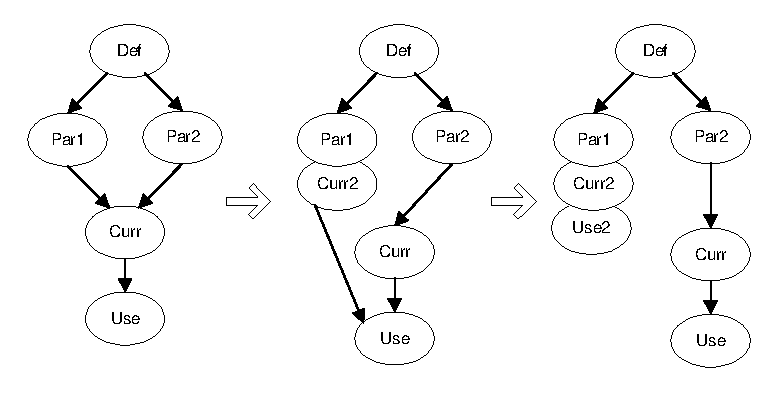
\includegraphics{figures/DuplicateBB.eps}
\centerfigend{fig-duplicateBB}{Duplicating BBs to ensure that each use of
a BasicBlock has a unique definition}

\subsection*{Duplicating a Basic Block}
When the parent of a basic block that needs to be duplicated is a fall-through
or a one-way jump BB, there is only one in-edge, so the RTLs for the current
BB are merely copied
to the end of the list of
RTLs in the parent BB. The parent BB then becomes the same type as the copied
BB, and has the same number of outedges. (The outedges are copied explicitly).
Copying of BBs is done with the clone() member function, to ensure ``deep''
copying. Otherwise, only the pointers to expressions are copied, not the
expressions themselves, and there will be problems when the expressions are
deleted (since the same expression will be deleted twice).

When the parent of a basic block that needs to be duplicated is a two-way BB,
the above method is not suitable. Instead, a new BB is created that is a clone
of the current BB, and the out-edge from the parent to the current BB is
changed to point to the new BB. (Note: this could be the first or ``true''
outedge, or it could be the second or ``false'' outedge). The back end must not
pay attention to the destination of the branch (which remains a faithful
decoding of the original source machine instruction), but rather to where the
BB that the out-edge points to.

In Figure~\ref{fig-duplicate-2way}(a), BB ``Curr'' has a parent BB (``Par1'')
which is a 2-way BB. In this case, a copy of ``Curr'' called ``Curr2'' is made
(Figure~\ref{fig-duplicate-2way}(b)), and the out-edge that used to point to
``Curr'' is changed to point to ``Curr2''. As before, this causes ``Curr2''
to have only one parent, but the successor of both ``Curr'' and ``Curr2''
(the BB ``Use'') now has two parents. When the process is applied to that BB,
we end up with the situation in Figure~\ref{fig-duplicate-2way}(c) where both
``Use'' and ``Use2'' have single paths to the defining BB (not shown).

\centerfigbegin
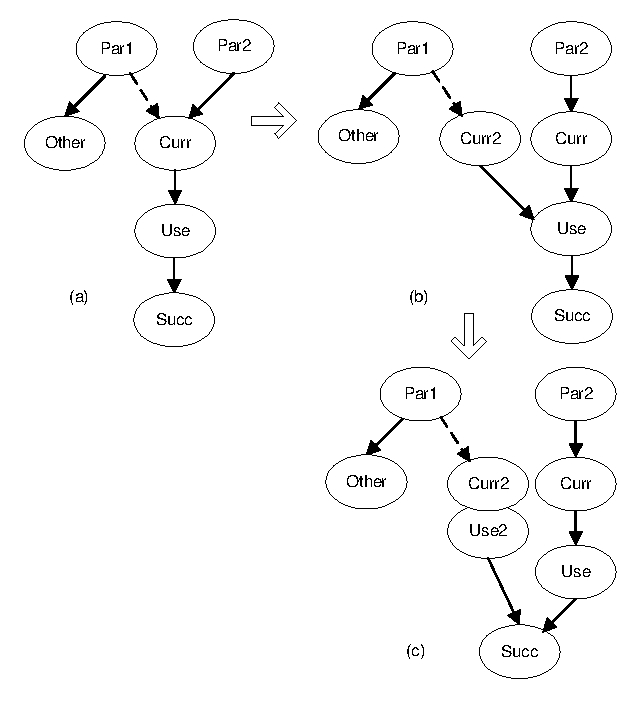
\includegraphics{figures/DuplicateBB2.eps}
\centerfigend{fig-duplicate-2way}{Duplicating a BB with a 2-way parent BB}


\section{Combining Uses and Definitions of Condition Codes}
\label{sec-comb-use-def}

Once unique pairs of CC uses and definitions are found, they must be converted
to a high level equivalent form.

\subsection{Conditional branches and set instructions}

Instructions defining the condition codes are divided into two classes:
``add-like'' and ``subtract-like''. The last RT of the RTL defining the
condition codes (which is expected to be an RTFlagCall\footnote{An object of
class RTFlagCall represents a call to a function that nominally sets the
condition codes for a family of instructions. For example, LOGICALFLAGS sets
the flags for the logical family of instructions.} object) is examined. If
the strings ``SUB'' or ``FFLAG''\footnote{Floating point compares are
considered to be always ``subtract like'', and SETFFLAGS is a typical
flag call function name for setting the floating point condition codes.}
are found in the name of the flag call function, the
instruction defining the condition codes is classified as ``subtract-like''.
Examples include compare instructions, and actual subtract instructions.
Otherwise, the instruction is classified as ``add-like''; examples include
logical instructions such as AND, multiply instructions, and actual ADD
instructions. It is therefore important that the flag call functions are
named appropriately in the SSL file (see section~\ref{sec-srd} for details).

Subtract-like definitions are handled by constructing a high level comparison
expression based on the operands of the comparison or subtraction, and the
type of branch or set instruction. For example,
\begin{verbatim}
 sub a, b, c    # Subtract b from a, result to c
 ...
 sge dest       # Set dest to 1 if "greater than or equals"
\end{verbatim}
has the following high level expression associated with it: ``a $>=$ b''.
The expression is stored in the HLJcond or HLScond object associated
with the RTL that uses the condition code. (The \texttt{setCondExpr} method is
used.)

It is not possible to use the operands directly, since in the final program,
a and b could be modified before the instruction that uses the condition codes.
A mechanism is needed to ``transport'' the condition code information from the
defining instruction to the using instruction. Variables (e.g. ``v12''),
unique to this definition-use pair, are used for this purpose.
Subtract-like definitions of the condition codes
require two such variables; one is needed for each operand.

The variables are copied from expressions passed to the HLFlagCall RT. This
ensures that the correct arguments are copied.

It is important to realise that the result of the subtract is \emph{not}
sufficient to store the result of an unsigned comparison; e.g. v12 = b \gtu\ c
and then branch if v12 \gtu\ 0. For example, 4 \gtu\ 3 and 4-3=1 \gtu\ 0. But
(using 8 bit operands) 204 \gtu\ 3, but 204-3 = 201 == -55, which is a negative
result. (Besides, everything is unsigned greater than 0, other than 0 itself).
The result of the unsigned comparison is in the carry flag, which is a sort of
9th bit of the result.  Therefore, it is not possible in general to save on
variables where unsigned comparisons are involved.

Example pairing:
\begin{verbatim}
10b84:  d0 07 bf e8        ld           [%fp - 24], %o0
10b88:  80 a4 00 08        cmp          %l0, %o0
10b8c:  1a 80 00 04        bgeu         0x10b9c
\end{verbatim}

translates to:

\begin{verbatim}
 v2=*(...);                 # %o0 is mapped to variable v2
 v30=v2;                    # Copy operand 1
 v29=r16;                   # Copy operand 2
 r0=(r16)-(v2);             # The compare, expressed as a subtract
                            #  (result is not used)
 v2=70656;                  # Delay slot instruction
 if (v29 >= v30) goto L11;  # Unsigned comparison
\end{verbatim}

By contrast, add-like definitions need only the result of the operation 
that sets the condition codes. It is an error to find unsigned branches 
or set instructions using the condition codes from an add-like definition. 
For example
\begin{verbatim}
 add a, b, c        # Add a and b, result to c
 ...
 jge dest           # Jump if "greater or equal" to dest
\end{verbatim}
becomes
\begin{verbatim}
c = a + b;
v12 = c;
 ...
if (v12 >= 0) goto dest;
\end{verbatim}

The exception to the above rules are the \texttt{HLJCOND\_JMI} and
\texttt{JLJCOND\_JPOS} branches. These can be used after add-like or after
subtract-like operations (usually a genuine subtract), but since they depend on
the result of the operation, they must be used in an add-like manner.
For example, from
\begin{verbatim}
10bec:  90 a2 20 01        subcc    %o0, 1, %o0
10bf0:  3c bf ff fa        bpos,a   0x10bd8
\end{verbatim}
we generate
\begin{verbatim}
r8=(r8)-(1);
v8=r8;
if ((v8)>=(0)) goto L3;
\end{verbatim}

The analysis code makes the assumptions that the last RT of the RTL defining
the condition codes is a flag call, and (for the above cases) that the second
last RT is an assignment to the result of the operation defining the flags.
Note that if there is a second branch that depends on the above operation,
the second last assignment will be to v8, but it still has the result of the
operation, so it will work correctly.

For other subtract-like operations and branches, it is assumed that the
first two operands (in order) of the flag call are the two operands being
compared (or subtracted). In other words, after
\begin{verbatim}
  x := y - z
  SUBFLAGS(a, b, ...)
\end{verbatim}
it is assumed that a is y and b is z.

As a result of these assumptions, the user is not free to use unusual
semantics in the SSL file. It is hard to imagine the above assumption not
being valid, but it should be kept in mind. In extreme cases, the result of
the operaton may have to be assigned to a temporary variable, then to
either the true destination or another temporary in the second last RT.

\subsection{Assignments that use Condition Codes}

When the instruction using a condition code is an assignment, it is usually
part of an idiomatic sequence.  Two idioms have so far been found and
implemented. The other class of instruction using the carry flag is as part
of multiword arithmetic (e.g. addcc, addx). It may be practical to implement
the multiword arithmetic pairs when the type analysis is able to cope with
variables in two registers; for now, these sequences generate an error message.
This example is from the Solaris 7 /usr/bin/awk:
\begin{verbatim}
142e8:  d2 07 20 00        ld           [%i4], %o1      # Load high half
142ec:  d6 07 20 04        ld           [%i4 + 4], %o3  # Load low half
...
                           # addcc sets flags according to result; add does not
14330:  b4 82 e0 01        addcc        %o3, 1, %i2     # Add 1 to low half
14334:  b2 42 60 00        addx         %o1, 0, %i1     # Add carry to top half
...
142d0:  f2 27 20 00        st           %i1, [%i4]
142d8:  f4 27 20 04        st           %i2, [%i4 + 4]
\end{verbatim}

Here, there are 64 bit integer quantities in the register pairs \%o1:\%o3,
and also \%i1:\%i2 (the colon represents concatenation).

The first idiomatic sequence is: ``compare 0 to a; use carry flag''. Arithmetic
assignment statements using the carry flag need no extra transformation; they
decode to RTLs which use the \%CF register (machine independent carry
flag). For example, \texttt{addx \%g0, 0, \%o3} decodes to
``r[10] := r[0] + 0 + \%CF''. (In the final C output of the translator, \%CF
is represented by the integer variable CF). Therefore, the only transformation
required is to ensure that each use has a unique definition, and to make an
appropriate assignment to \%CF.

Since subtracting any value from zero will generate a carry, unless that value
is zero, comparing 0 to X is equivalent to setting the carry flag only if X
is non-zero. In other words,
compare 0 to X is transformed to ``\%CF = (X != 0)''. An appropriate
assignment RT (i.e. an object of class RTAssgn) is created, and appended to the
list of RTs for the RTL defining the flags. For example:
\begin{verbatim}
10aec:  80 a0 00 0b        cmp          %g0, %o3        # %g0 is always 0
10af0:  94 60 3f ff        subx         %g0, -1, %o2    # Make use of %CF
10af8:  96 40 20 00        addx         %g0, 0, %o3     # Another use of %CF
\end{verbatim}
transforms to
\begin{verbatim}
         # Variable v5 represents register %o3 for this procedure
00010aec *32* r[0] := -v5           # The compare, expressed as a subtract
         *32* %CF := v5 ~= 0        # Generated assignment
         SUBFLAGS( r[0], v5, r[0] )
00010af0 *32* v4 := -%CF + 1        # Register %o2 is held in variable v4
00010af4 *32* v5 := %CF             # Register %o3 is held in variable v5
\end{verbatim}
In C, this becomes
\begin{verbatim}
        r0=-(v5);
        CF=(v5)!=(0);
        v4=(-(CF))+(1);
        v5=CF;
\end{verbatim}


The second idiomatic sequence is similar: ``compare X to Y; use carry flag''.
This is transformed to ``\%CF = X \ltu\ Y'' (where \ltu\ represents ``unsigned
less than''). After subtracting Y from X, a carry will be generated if and only
if Y is greater than x (with both X and Y considered as unsigned quantities).
In other words, after cmp X, Y the carry flag represents the logical expression
X \ltu\ Y.

\section{Complex example}

Despite the apparent simplicity of the above, real code can be surprisingly
complex. The following SPARC code is from the 126.gcc Spec benchmark, generated
from the last 4 lines of C here:

\begin{verbatim}
  int unsignedp = TREE_UNSIGNED (index_type);
  typedef rtx rtx_function ();
  rtx_function *gen_bgt_pat = unsignedp ? gen_bgtu : gen_bgt;
  rtx_function *gen_bge_pat = unsignedp ? gen_bgeu : gen_bge;
  rtx_function *gen_blt_pat = unsignedp ? gen_bltu : gen_blt;
  rtx_function *gen_ble_pat = unsignedp ? gen_bleu : gen_ble;
\end{verbatim}

The addresses of the eight functions (e.g. \texttt{gen\_bgtu}) are set up in
registers like \texttt{\%i2} and stack memory like \texttt{[\%sp + 144]}
in earlier code that is not relevant to the analysis.

\begin{verbatim}
7834c:  80 90 00 1b        orcc         %g0, %i3, %g0
78350:  02 80 00 04        be           0x78360
78354:  a8 10 00 1a        mov          %i2, %l4
78358:  10 80 00 02        ba           0x78360
7835c:  a8 10 00 19        mov          %i1, %l4
78360:  22 80 00 04        be,a    0x78370
78364:  e4 03 a0 90        ld           [%sp + 144], %l2
78368:  10 80 00 02        ba           0x78370
7836c:  e4 03 a0 94        ld           [%sp + 148], %l2
78370:  22 80 00 04        be,a    0x78380
78374:  e2 03 a0 98        ld           [%sp + 152], %l1
78378:  10 80 00 02        ba           0x78380
7837c:  e2 03 a0 9c        ld           [%sp + 156], %l1
78380:  02 80 00 04        be           0x78390
78384:  90 10 00 1c        mov          %i4, %o0
78388:  10 80 00 03        ba           0x78394
7838c:  a0 10 00 1d        mov          %i5, %l0
78390:  e0 03 a0 a0        ld           [%sp + 160], %l0
78394:  92 10 00 15        mov          %l5, %o1
\end{verbatim}

The orcc instruction at the top is the definition for the following conditional
branch, and also three more branches. Because of the two-way BBs between the
definition and the conditional branches, there are a lot of BB duplications
required to translate this code.

There are also several ``orphan'' basic blocks generated as a result of
untangling the delay slots in the above. The code above generates some
23 basic blocks, as shown in Figure~\ref{fig-complex-example}.

\centerfigbegin
{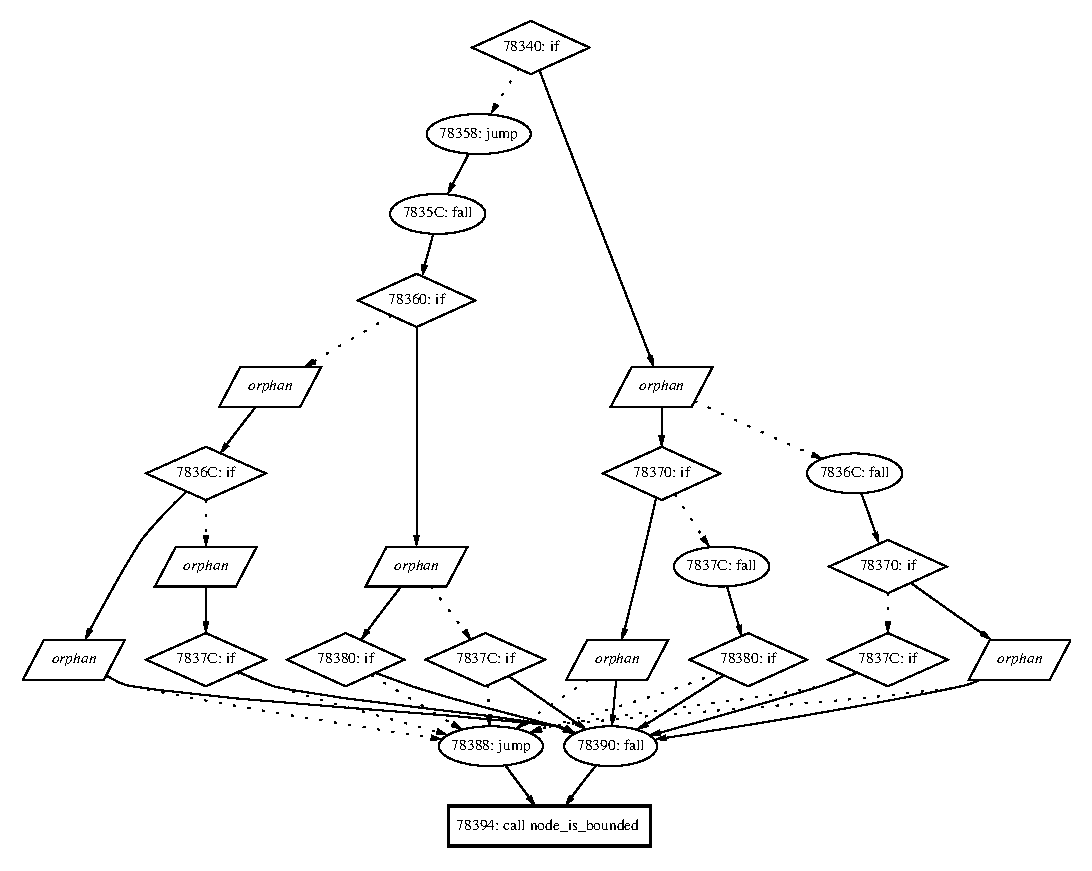
\includegraphics{figures/complex_example.eps}}
\centerfigend{fig-complex-example}{BBs generated for the complex example}
      % matching condition code definitions and uses

  	
\chapter{Transformations of Delayed Transfers of Control}
\label{ch-delay}

{\small
\begin{flushright}
Design: Norman and Cristina [c.98]; Implementation: Mike [c.98-99]; Documentation: Norman, Cristina [Sep 99]
\end{flushright}
}

This chapter is an updated version of Technical Report 440, Department of 
Computer Science and Electrical Engineering, The University of 
Queensland, December 1998.  A more up to date version, including 
application of this algorithm to the removal of PA-RISC delayed branches
will be part of a Sun Microsytems Laboratories Technical Report series  
(expected, early 2002). 
 

% l2h ignore special {% ===> this file was generated automatically by noweave --- better not edit it

%\ifx\afour\undefined
%  \documentclass[letterpaper]{elsart}
%  \let\sizeinfo\relax
%\else 
%  \documentclass[a4paper]{elsart}
%  \special{papersize=210mm,297mm} % put dvips into a4 automagically
%  \def\sizeinfo{A4 }
%\fi

%\usepackage{nchicago}

% l2h substitution bullet *
% l2h substitution and and
% l2h ignore active


\makeatletter
\def\@citex[#1]#2{%
  \let\@citea\@empty
  \@cite{\@for\@citeb:=#2\do
        {\@citea\def\@citea{,\penalty\@m\ }%
         \edef\@citeb{\expandafter\@firstofone\@citeb}%
         \if@filesw\immediate\write\@auxout{\string\citation{\@citeb}}\fi
         \@ifundefined{b@\@citeb}{\mbox{\reset@font\bfseries ?}%
           \G@refundefinedtrue
           \@latex@warning
             {Citation `\@citeb' on page \thepage \space undefined}}%
           {\citebox{\csname b@\@citeb\endcsname}}}}{#1}}
\let\citebox\hbox
\makeatother

\renewcommand\gets{\mathrel{:=}}

\newcommand\opentab{\addtolength{\extrarowheight}}
% l2h ignore catcode ==
% l2h let gdef def

% l2h substitution hatform ^
% l2h ignore markboth {{

% l2h ignore opentab {

% l2h substitution presigmap sigma'
% l2h ignore productionglue
% l2h substitution qquad &nbsp;&nbsp;&nbsp;&nbsp;&nbsp;

\newif\iffullpaper
\fullpapertrue


% l2h argblock calexp E[ ]
% l2h argblock cmd E[ ]


\newcommand\calexp[1]{{\mathcal E}[\![#1]\!]}
\newcommand\cmd[1]{{\mathcal C}[\![#1]\!]}
\newcommand\pc{\mathit{PC}}

%\usepackage{array,tabularx,grammar}

% l2h letenv production quote

\newif\iftr
\trfalse % this is not the tech report

\newcolumntype{Y}{>{\raggedright\arraybackslash}X}


%\usepackage{noweb}
\let\originalprime='
\def\setupcode{\catcode`\ =10 \catcode`\'=12 \mathcode`\'="8000 \regressprime}
{\catcode`\'=\active 
 \makeatletter
 \gdef\regressprime{\def'{^\bgroup\prim@s}}
}
\let\Tt\relax


% l2h substitution div div
% l2h substitution mod mod

\overfullrule=10pt

\noweboptions{shortxref}
\def\nwdocspar{\vskip0pt plus1.5in\penalty-400\vskip0pt plus -1.5in}
%\def\nwdocspar{\par\penalty-1000}
\def\nwendcode{\endtrivlist\endgroup} % ditches filbreak
%\def\nwendcode{\endtrivlist\endgroup\vskip\nwextraglue} % page tuning

\newcommand{\fig}[1]{Figure~\ref{fig:#1}}

\newcommand\sfilbreak[1]{\vskip 0pt plus#1\penalty-200\vskip 0pt plus -#1}

\setcounter{secnumdepth}{2}

\let\orghbox=\hbox
\newcommand\nohbox{\let\hbox=\orghbox\relax}



%% \pagestyle{myheadings}
%% \catcode`\$=10 % make $ a blank space
%% \catcode`\:=10 % make : a blank space
%% \newcommand\rcsrevision{$Revision: 1.4 $}
%% \catcode`\$=3 % dollar sign is math shift
%% \catcode`\:=12
%% \markboth{\rcsrevision: \sizeinfo Draft of \today}{\rcsrevision: \sizeinfo Draft of \today}
%% 
%% \pagestyle{plain}

\def\remark#1{\marginpar{\raggedright\hbadness=10000
        \def\baselinestretch{0.8}\scriptsize
        \it #1\par}}

\let\hatform\overline

\let\nwpphat=\hatform

The fundamental steps in binary translation are
distinguishing code from data, mapping data from source to
target, and translating instructions.
Translating instructions presents few problems, except
when the source instruction set 
has features not present in typical compiler intermediate codes.
The most common such feature is the delayed branch.

Standard code-generation technology can handle delayed branches in the
target language, but not in the source.
Translating delayed branches can involve tricky case
analyses to figure out what happens if there is a branch instruction in
a delay slot.
This chapter presents a disciplined method for deriving such case analyses.
The method identifies problematic cases,
shows the translations for the non-problematic cases, and gives
confidence that all cases are considered.
The method also applies to other tools that analyze machine instructions.

We begin by writing a very simple interpreter for the source machine.
It specifies, at the register-transfer level, how the source machine
executes instructions, including delayed branches. We then transform
the interpreter into an interpreter for a target machine without
delayed branches.
To maintain the semantics of the program being interpreted, we 
simultaneously transform the sequence of source-machine instructions
into a sequence of target-machine instructions.
The transformation of the instructions becomes our
algorithm for binary translation.

We show the translation is correct by using a correspondence between
source and target states, and showing if the source and target
machines begin execution in corresponding states, they reach new
corresponding states in a few instructions.


\renewcommand\opencite[1]{{\let\citebox=\relax\cite{#1}}}

A quick reading of this chapter might suggest that the problem we solve
is trivial.
To build a flow graph representing a binary program,
why not simply convert the delayed branch to a non-delayed branch and
push the instruction in the delay slot along zero, one, or both
sucessor edges?
(The set of successors that should get copies of the instruction in
the delay slot depends on whether the delayed branch
``annuls'' that instruction.)
This simple approach is in fact correct, \emph{except} when the
instruction in the delay slot is itself a delayed branch.
In that case, the ``pushing'' approach fails to execute the
instruction that is the target of the first branch.
The methods in this paper translate this case correctly.
In practice, such cases occur rarely in user code, but they are
recommended in kernel code as a way of returning from interrupts or
otherwise switching contexts \cite[\S B.26]{sparc:architecture}.


\section{Semantic framework}

Rather than translate source-machine instructions directly into target-machine
instructions, we translate source instructions into register transfer
lists (RTLs), transform the RTLs, optimize the RTLs, and translate the
RTLs into target-machine instructions.
RTLs provide a uniform framework that can express source instructions,
target instructions, and their interpretations by the source and
target processors.

\subsection{Register transfer lists}

Our RTL formalism is designed for use in tools and component
generators, and it makes machine-dependent
computation explicit \opencite{ramsey:embedded}.
For this paper, we use a simplified version specified using an imperative syntax:
\begin{production}{rtl}%figure
\optional{\nt{effect} \sequence{\lit\vbar\ \nt{effect}}}
&Multiple assignment
\end{production}
\productionglue
\begin{production}{effect}%figure
\optional{\nt{exp} {{\Tt{}\(\mathbin{\rightarrow}\)}}} \nt{location} := \nt{exp}&
Guarded assignment
\end{production}
\productionglue
\begin{production}{exp}%figure
\term{constant}&Constant
| \nt{location}&Fetch from a location
| \nt{exp} \nt{binop} \nt{exp}&Binary RTL operator
| \nt{operator} \lit( \nt{explist} \lit)&RTL operator
\end{production}
A register transfer list is a list of guarded effects.
Each effect represents the transfer of a value into a storage
location,\footnote{Storage locations represent not only memory but
also registers and other processor state.}
 i.e., a store
operation.
The transfer takes place only if the guard (an expression) evaluates
to \textbf{true}.
Effects in a list take place simultaneously, as in
Dijkstra's multiple-assignment statement; an RTL represents a single
change of state.
%%For example, one RTL can specify a swap instruction without
%%introducing bogus temporaries.

Values are computed by expressions without
side effects.
Eliminating side effects simplifies analysis and transformation.
Expressions may be integer constants, fetches from locations, or
applications of \emph{RTL operators} to lists of expressions.
RTL operators are pure functions on values.

For purposes of this paper, we assume that locations are single cells
in a mutable store, although the RTL formalism supports a more general
view that makes byte order explicit.
\iffalse
Locations may be single cells or aggregates of consecutive
cells within a storage space.
Aggregation generalizes the idea of byte order, specifying a bijection
between a contiguous sequence of $k$ $n$-bit values and a single
$w$-bit value, where $w = kn$.\footnote{$w$ and $n$ are mnemonic for
``wide'' and ``narrow.''}
\fi

\iffullpaper
As an example of a typical RTL, consider a SPARC load instruction
using the displacement 
addressing mode, written in the SPARC  assembly language as
\begin{verbatim}
  ld [%sp-12], %i0
\end{verbatim}
The effect of this load instruction might be written
\nwenddocs{}\nwbegincode{2}\moddef{RTL for sample instruction}\endmoddef\nwstartdeflinemarkup\nwenddeflinemarkup
\(\$r[24] \mathrel{:=} \$m[\$r[14]+{\mathit{sx}}(\mathord{-}12)]\)
\nwendcode{}\nwbegindocs{3}because the stack pointer is register~14 and register \texttt{\%i0} is
register~24.
The notation {\Tt{}\(\$\)}\emph{space}\texttt{[}\emph{address}\texttt{]}
specifies a cell in a mutable store.
The {\Tt{}\({\mathit{sx}}\)} operator sign-extends the 13-bit immediate constant {\Tt{}\(\mathord{-}12\)}
so it can be added to the 32-bit value fetched from register~14.

The load instruction not only loads a value into register~24; it also advances
the program counter to point to the next instruction.
Changing the program counter is intimately connected with branching;
we separate the effect on the
program counter in order to give it special treatment.
\else
\emph{The full paper shows and explains an example RTL.}
\fi

\subsection{Processor state for delayed branches}

A processor executing straight-line code executes one instruction
after another, in sequence.
A delayed-branch instruction causes the processor to depart from that
sequence, but not immediately.
When the processor executes an instruction~{\Tt{}\(I\)} that causes a delayed
branch to a location 
{\Tt{}\({\mathit{target}}\)}, the processor {first} executes {\Tt{}\(I\)}'s successor,
{then} executes the instruction located at {\Tt{}\({\mathit{target}}\)}.
The location holding {\Tt{}\(I\)}'s successor is called {\Tt{}\(I\)}'s ``delay
slot.''
On some machines, like the SPARC,
the instruction~{\Tt{}\(I\)} can
``annul'' its successor, in which case the successor is
\emph{not} executed, but instead the processor stalls for a cycle
before transferring control to {\Tt{}\({\mathit{target}}\)}.

To model delayed branches with annuls, we use
three pieces of processor state:
\begin{itemize}
\item[{}{\Tt{}\({\mathit{PC}}\)}{}] is the program counter, which identifies the
instruction about to be executed.
\item[{}{\Tt{}\({\mathit{nPC}}\)}{}] is the ``next program counter,'' which identifies the
instruction to be executed after the current instruction.
\item[{}{\Tt{}\({\mathit{annul}}\)}{}] is the ``annul status,'' which determines
whether the processor executes the instruction at~{\Tt{}\({\mathit{PC}}\)} or ignores
it.%
\footnote{\iffullpaper
It is crucial to distinguish the {\Tt{}\({\mathit{annul}}\)} status, which is
part of 
the processor state, from the \texttt{a}~bit found in the binary
representations of some branch instructions.
The interpretation of the {\Tt{}\({\mathit{annul}}\)} status is trivial: it tells
directly whether to execute an instruction.
The interpretation of the \texttt{a}~bit (when present) is more involved,
because there are special rules for some instructions.
We abstract away from these special rules by associating with each
instruction~{\Tt{}\(I\)} a predicate~{\Tt{}\(a_I\)} (not necessarily a single bit) that
tells the processor 
whether to annul the instruction's successor.
\else
\emph{The full paper notes the distinction between {\Tt{}\({\mathit{annul}}\)} and the
\texttt{a}~bit found in some branch instructions.}%
\fi
}
\end{itemize}
In this model, a delayed control transfer is represented by an
assignment to~{\Tt{}\({\mathit{nPC}}\)}.
For example, a SPARC call instruction simultaneously
assigns the target address to~{\Tt{}\({\mathit{nPC}}\)}
and the current {\Tt{}\({\mathit{PC}}\)} to register~15:
\nwenddocs{}\nwbegincode{4}\moddef{RTL for call}\endmoddef\nwstartdeflinemarkup\nwenddeflinemarkup
\({\mathit{nPC}} \mathrel{:=} {\mathit{target}} \mathrel{|} \$r[15] \mathrel{:=} {\mathit{PC}}\)
\nwendcode{}\nwbegindocs{5}The {\Tt{}\({\mathit{target}}\)} address in the semantics is
distinct from the \texttt{target} field in the binary representation of the
call instruction.
In the case of the SPARC, we abstract away from the rule that says the
target 
address is computed by extending the \texttt{target} field on the
right with zeroes.

A call transfers control unconditionally; we represent a conditional
branch by a guarded assignment to {\Tt{}\({\mathit{nPC}}\)}.
The \texttt{BNE} (branch not equal) instruction tests the {\Tt{}\(Z\)}~(zero)
bit in the condition codes:
\nwenddocs{}\nwbegincode{6}\moddef{rtl for conditional branch \texttt{BNE}}\endmoddef\nwstartdeflinemarkup\nwenddeflinemarkup
\(\lnot  Z \mathbin{\rightarrow} {\mathit{nPC}} \mathrel{:=} {\mathit{target}}\)
\nwendcode{}\nwbegindocs{7}Again we abstract the computation of the target address relative to
the location of the instruction.
\nwenddocs{}\nwbegindocs{8}\nwdocspar
\subsection{A canonical form of RTLs}
To isolate the part of instruction semantics that is relevant to
control flow, we put RTLs into the following canonical form:
\nwenddocs{}\nwbegincode{9}\moddef{RTL for generic instruction \code{}I\edoc{}}\endmoddef\nwstartdeflinemarkup\nwenddeflinemarkup
\(b_I \mathbin{\rightarrow} {\mathit{nPC}} \mathrel{:=} {\mathit{target}}_I \mathrel{|} {\mathit{annul}} \mathrel{:=} a_I \mathrel{|} I_c\)
\nwendcode{}\nwbegindocs{10}We interpret this form as follows:
\begin{itemize}
\item [{}{\Tt{}\(b_I\)}{}] is a predicate that tells whether {\Tt{}\(I\)}~branches.
It is an \emph{expression}, not a constant or a field of the
instruction.
For non-branching instructions, {\Tt{}\(b_I\)}~is {\Tt{}\(\textbf{false}\)}.
For calls and
unconditional branches, {\Tt{}\(b_I\)} is {\Tt{}\(\textbf{true}\)}.
For conditional branches, {\Tt{}\(b_I\)} is some other expression, the value of
which depends on the state of the machine (e.g., on the values of
the condition codes).
\item [{}{\Tt{}\({\mathit{target}}_I\)}{}] is an {expression} that identifies the
target address to which {\Tt{}\(I\)}~may branch.
(If {\Tt{}\(b_I\)} is {\Tt{}\(\textbf{false}\)}, {\Tt{}\({\mathit{target}}_I\)} is arbitrary.)
For calls and PC-relative branches, {\Tt{}\({\mathit{target}}_I\)} is a constant that
statically identifies a target address.
For indirect branches, {\Tt{}\({\mathit{target}}_I\)} may be a more complex expression,
e.g., one that fetches an address stored in a register.
\item [{}{\Tt{}\(a_I\)}{}] is a predicate that tells whether {\Tt{}\(I\)}~annuls its
successor. 
It is an expression, {not} the value of the \texttt{a}~bit in an
instruction's representation.
For most instructions, {\Tt{}\(a_I\)} is {\Tt{}\(\textbf{false}\)}.
For conditional branches, {\Tt{}\(a_I\)} may be more complicated.
For example,  the SPARC \texttt{BNE} instruction annuls its successor
if the \texttt{a} bit is set and if the branch is not taken, so {\Tt{}\(a_I\)} is
\mbox{{\Tt{}\(\mathtt{a} \ne  0 \land  Z\)}}.
\item [{}{\Tt{}\(I_c\)}{}] is an RTL that represents {\Tt{}\(I\)}'s ``computational
effect.''
{\Tt{}\(I_c\)} may be empty, or it may contain guarded assignments that do
not change {\Tt{}\({\mathit{annul}}\)}, {\Tt{}\({\mathit{nPC}}\)}, or {\Tt{}\({\mathit{PC}}\)}.
Typical RISC instructions change control flow or perform computation,
but not both, so {\Tt{}\(I_c\)} tends to be non-empty only when {\Tt{}\(b_I\)}
and {\Tt{}\(a_I\)} are {\Tt{}\(\textbf{false}\)}.
On CISC architectures, however, an instruction like ``decrement and
skip if zero'' might have both  non-empty {\Tt{}\(I_c\)} (the decrement) and
a nontrivial {\Tt{}\(b_I\)} (the test for zero).
\end{itemize}
An instruction can be expressed in this canonical form if, when
executed, it branches to
at most one {\Tt{}\({\mathit{target}}\)}.%
\footnote{And of course if the machine uses delayed branches.}
This is true of all instructions on all architectures with which we
are 
familiar, including indirect-branch instructions (although the value
 of {\Tt{}\({\mathit{target}}\)} may be different on different executions of an indirect
branch).

Here are a few example RTLs in canonical form;
SPARC assembly language appears on the left, RTLs on the right.
{\Tt{}\textbf{skip}} is the empty~RTL.
\begin{quote}%figure
\begin{tabular}{@{}ll@{}}
\multicolumn2{@{}l}{\texttt{add rs1, rs2, rd}}\\
\multicolumn2{@{}l}{\qquad  
{\Tt{}\(\textbf{false} \mathbin{\rightarrow} {\mathit{nPC}} \mathrel{:=} {\mathit{any}} \mathrel{|} {\mathit{annul}} \mathrel{:=} \textbf{false} \mathrel{|} \$r[\mathtt{rd}] \mathrel{:=} \$r[\mathtt{rs1}] + \$r[\mathtt{rs2}]\)}}\\
\texttt{ba,a addr}&{\Tt{}\(\textbf{true} \mathbin{\rightarrow} {\mathit{nPC}} \mathrel{:=} \mathtt{addr} \mathrel{|} {\mathit{annul}} \mathrel{:=} \textbf{true} \mathrel{|}\){\ }\textbf{skip}}\\
\texttt{call addr}&{\Tt{}\(\textbf{true} \mathbin{\rightarrow} {\mathit{nPC}} \mathrel{:=} \mathtt{addr} \mathrel{|} {\mathit{annul}} \mathrel{:=} \textbf{false} \mathrel{|} \$r[15] \mathrel{:=} {\mathit{PC}}\)}\\
\end{tabular}\kern-20pt
\end{quote}

\nwenddocs{}\nwbegindocs{11}\nwdocspar
\subsection{Instruction decoding and execution on two platforms}
Given this canonical form for instructions, we represent instruction
decoding using a {\Tt{}\textbf{let}}-binding notation:
\nwenddocs{}\nwbegincode{12}\moddef{instruction decoding}\endmoddef\nwstartdeflinemarkup\nwenddeflinemarkup
\textbf{let}{\ }\((b_I \mathbin{\rightarrow} {\mathit{nPC}} \mathrel{:=} {\mathit{target}}_I \mathrel{|} {\mathit{annul}} \mathrel{:=} a_I \mathrel{|} I_c) \equiv  {\mathit{src}}[{\mathit{PC}}]\)
\textbf{in}{\ }{\ }\(\ldots\)
\textbf{end}
\nwendcode{}\nwbegindocs{13}The {\Tt{}\textbf{let}} construct binds {\Tt{}\(b_I\)}, {\Tt{}\({\mathit{target}}_I\)},
{\Tt{}\(a_I\)}, and {\Tt{}\(I_c\)}, which together determine the
semantics of the instruction~{\Tt{}\(I\)} found in the source memory~{\Tt{}\({\mathit{src}}\)}.
\iffullpaper
This {\Tt{}\textbf{let}}-binding represents not only the process of using the
binary representation to identify the instruction and its operands,
but also the abstraction from that representation into the RTL semantics.
This abstraction from binary representation to semantics can be done
statically, at 
binary-translation time; it can even be automated based on a
combination of machine descriptions
\opencite{ramsey:specifying,ramsey:embedded}.
\fi
\nwenddocs{}\nwbegindocs{14}\nwdocspar
The source-machine execution loop
decodes an instruction and executes it as follows:
\nwenddocs{}\nwbegincode{15}\moddef{sparc execution loop}\endmoddef\nwstartdeflinemarkup\nwenddeflinemarkup
\textbf{fun}{\ }\({\mathit{loop}} () \equiv \)
{\ }{\ }\textbf{let}{\ }\((b_I \mathbin{\rightarrow} {\mathit{nPC}} \mathrel{:=} {\mathit{target}}_I \mathrel{|} {\mathit{annul}} \mathrel{:=} a_I \mathrel{|} I_c) \equiv  {\mathit{src}}[{\mathit{PC}}]\)
{\ }{\ }\textbf{in}{\ }{\ }\textbf{if}{\ }\({\mathit{annul}}\){\ }\textbf{then}
{\ }{\ }{\ }{\ }{\ }{\ }{\ }{\ }{\ }\({\mathit{PC}} \mathrel{:=} {\mathit{nPC}} \mathrel{|} {\mathit{nPC}} \mathrel{:=} {\mathit{succ}}_s({\mathit{nPC}}) \mathrel{|} {\mathit{annul}} \mathrel{:=} \textbf{false}\)
{\ }{\ }{\ }{\ }{\ }{\ }\textbf{else}{\ }\textbf{if}{\ }\([\![b_I]\!]\){\ }\textbf{then}
{\ }{\ }{\ }{\ }{\ }{\ }{\ }{\ }{\ }\({\mathit{PC}} \mathrel{:=} {\mathit{nPC}} \mathrel{|} {\mathit{nPC}} \mathrel{:=} [\![{\mathit{target}}_I]\!]  \mathrel{|} [\![I_c]\!] \mathrel{|} {\mathit{annul}} \mathrel{:=} [\![a_I]\!]\)
{\ }{\ }{\ }{\ }{\ }{\ }\textbf{else}
{\ }{\ }{\ }{\ }{\ }{\ }{\ }{\ }{\ }\({\mathit{PC}} \mathrel{:=} {\mathit{nPC}} \mathrel{|} {\mathit{nPC}} \mathrel{:=} {\mathit{succ}}_s({\mathit{nPC}}) \mathrel{|} [\![I_c]\!] \mathrel{|} {\mathit{annul}} \mathrel{:=} [\![a_I]\!]\)
{\ }{\ }{\ }{\ }{\ }{\ }\textbf{fi}
{\ }{\ }{\ }{\ }{\ }{\ }\(; {\mathit{loop}}()\)
{\ }{\ }\textbf{end}
\nwendcode{}\nwbegindocs{16}We specify the repeated execution of the processor loop as a tail
call, rather than as a loop, because that simplifies the
program transformations to follow.
\nwenddocs{}\nwbegindocs{17}\nwdocspar
The notation {\Tt{}\([\![\bullet ]\!]\)} represents execution; for example,
{\Tt{}\([\![b_I]\!]\)} is the value of the branch condition, given the current
state of the machine.
Executing the computational effect {\Tt{}\([\![I_c]\!]\)} changes the state of the machine.
\nwenddocs{}\nwbegindocs{18}\nwdocspar
The function {\Tt{}\({\mathit{succ}}_s\)} abstracts over the details of identifying
the successor instruction on the source machine; {\Tt{}\({\mathit{succ}}_t\)} finds the
successor on the target machine.
In both cases, {\Tt{}\({\mathit{succ}}\)} is computed as part of instruction decoding.
\nwenddocs{}\nwbegindocs{19}\nwdocspar
Our example target, the Pentium, has neither delayed branches nor
annulling, so it has a simpler canonical form and a simpler execution
loop:
\nwenddocs{}\nwbegincode{20}\moddef{Pentium execution loop}\endmoddef\nwstartdeflinemarkup\nwenddeflinemarkup
\textbf{fun}{\ }\({\mathit{simple}} () \equiv \)
{\ }{\ }\textbf{let}{\ }\((b_I \mathbin{\rightarrow} {\mathit{PC}} \mathrel{:=} {\mathit{target}}_I \mathrel{|} I_c) \equiv  {\mathit{tgt}}[{\mathit{PC}}]\)
{\ }{\ }\textbf{in}{\ }{\ }\textbf{if}{\ }\([\![b_I]\!]\){\ }\textbf{then}
{\ }{\ }{\ }{\ }{\ }{\ }{\ }{\ }\({\mathit{PC}} \mathrel{:=} [\![{\mathit{target}}_I]\!] \mathrel{|} [\![I_c]\!]\)
{\ }{\ }{\ }{\ }{\ }{\ }\textbf{else}
{\ }{\ }{\ }{\ }{\ }{\ }{\ }{\ }\({\mathit{PC}} \mathrel{:=} {\mathit{succ}}_t({\mathit{PC}}) \mathrel{|} [\![I_c]\!]\)
{\ }{\ }{\ }{\ }{\ }{\ }\textbf{fi}
{\ }{\ }{\ }{\ }{\ }{\ }\(; {\mathit{simple}}()\)
{\ }{\ }\textbf{end}
\nwendcode{}\nwbegindocs{21}\nwdocspar




\subsection{Strategy for translating delayed branches}

Both our formalism and
the SPARC architecture manual give a clear semantics of delayed
branches in terms of {\Tt{}\({\mathit{PC}}\)}, {\Tt{}\({\mathit{nPC}}\)}, and {\Tt{}\({\mathit{annul}}\)}.
To get an efficient target program, however, we wish \emph{not} to
represent the source {\Tt{}\({\mathit{PC}}\)}, {\Tt{}\({\mathit{nPC}}\)}, and {\Tt{}\({\mathit{annul}}\)} explicitly, but to
make all three \emph{implicit} in the value of the target~{\Tt{}\({\mathit{PC}}\)}.
How to do this based on the information in the architecture manual is
not immediately obvious, but our semantic framework enables a new technique.
We transform {\Tt{}\({\mathit{loop}}\)}, eliminating {\Tt{}\({\mathit{nPC}}\)} and {\Tt{}\({\mathit{annul}}\)} wherever
possible, so that (almost all of) {\Tt{}\({\mathit{loop}}\)} can be expressed using only
the~{\Tt{}\({\mathit{PC}}\)}.
%%This transformation leads to suitable changes in the sequence of
%%instructions executed, thus guiding a transformation from {\Tt{}\({\mathit{src}}\)} to {\Tt{}\({\mathit{tgt}}\)}.
%%This latter transformation is an algorithm for binary translation of
%%delayed-branch instructions.


% l2h substitution src s-sigma-
% l2h substitution tgt t-sigma-

\newcommand\presigma[1]{\mathord{{}^{#1}\sigma}}
\newcommand\presigmap[1]{\mathord{{}^{#1}\sigma'}}
\newcommand\src[1]{\presigma{s}_{#1}}
\newcommand\tgt[1]{\presigma{t}_{#1}}


\section{Transforming the execution loop}

We wish to develop a translation function that we can point at a
location {\Tt{}\({\mathit{src}}[{\mathit{pc}}_s]\)} and that will produce suitable instructions at a
corresponding target location {\Tt{}\({\mathit{tgt}}[{\mathit{pc}}_t]\)}.
We cannot simply have {\Tt{}\({\mathit{pc}}_t = {\mathit{pc}}_s\)}; source program counters
cannot be identical to target program counters, because 
source and target instruction sequences may be different sizes.
During translation, we build {\Tt{}\({\mathit{codemap}}\)}, a map that relates program
counters on the two machines, so {\Tt{}\({\mathit{pc}}_t = {\mathit{codemap}}({\mathit{pc}}_s)\)}.

We assume that
when the source processor starts executing code at {\Tt{}\({\mathit{src}}[{\mathit{pc}}_s]\)}, it
is not in the middle of a delayed
or annulled branch, or formally,
\begin{quote}
{\Tt{}\({\mathit{annul}} = \textbf{false} \land  {\mathit{nPC}} = {\mathit{succ}}_s({\mathit{PC}})\)}.
\end{quote}
Software conventions guarantee that
the processor will be in such a state at a program's start location
and at procedure entry points.
\nwenddocs{}\nwbegindocs{22}\nwdocspar
We begin our transformation by
defining a function {\Tt{}\({\mathit{stable}}\)} that can be substituted for {\Tt{}\({\mathit{loop}}\)}
whenever {\Tt{}\({\mathit{annul}} = \textbf{false} \land  {\mathit{nPC}} = {\mathit{succ}}_s({\mathit{PC}})\)}.
\nwenddocs{}\nwbegincode{23}\moddef{stable execution loop}\endmoddef\nwstartdeflinemarkup\nwenddeflinemarkup
\textbf{fun}{\ }\({\mathit{stable}} () \equiv \)
{\ }{\ }\({\mathit{annul}} \mathrel{:=} \textbf{false} \mathrel{|} {\mathit{nPC}} \mathrel{:=} {\mathit{succ}}_s({\mathit{PC}});\)
{\ }{\ }\textbf{let}{\ }\((b_I \mathbin{\rightarrow} {\mathit{nPC}} \mathrel{:=} {\mathit{target}}_I \mathrel{|} {\mathit{annul}} \mathrel{:=} a_I \mathrel{|} I_c) \equiv  {\mathit{src}}[{\mathit{PC}}]\)
{\ }{\ }\textbf{in}{\ }{\ }\textbf{if}{\ }\({\mathit{annul}}\){\ }\textbf{then}
{\ }{\ }{\ }{\ }{\ }{\ }{\ }{\ }{\ }\({\mathit{PC}} \mathrel{:=} {\mathit{nPC}} \mathrel{|} {\mathit{nPC}} \mathrel{:=} {\mathit{succ}}_s({\mathit{nPC}}) \mathrel{|} {\mathit{annul}} \mathrel{:=} \textbf{false}\)
{\ }{\ }{\ }{\ }{\ }{\ }\textbf{else}{\ }\textbf{if}{\ }\([\![b_I]\!]\){\ }\textbf{then}
{\ }{\ }{\ }{\ }{\ }{\ }{\ }{\ }{\ }\({\mathit{PC}} \mathrel{:=} {\mathit{nPC}} \mathrel{|} {\mathit{nPC}} \mathrel{:=} [\![{\mathit{target}}_I]\!]  \mathrel{|} [\![I_c]\!] \mathrel{|} {\mathit{annul}} \mathrel{:=} [\![a_I]\!]\)
{\ }{\ }{\ }{\ }{\ }{\ }\textbf{else}
{\ }{\ }{\ }{\ }{\ }{\ }{\ }{\ }{\ }\({\mathit{PC}} \mathrel{:=} {\mathit{nPC}} \mathrel{|} {\mathit{nPC}} \mathrel{:=} {\mathit{succ}}_s({\mathit{nPC}}) \mathrel{|} [\![I_c]\!] \mathrel{|} {\mathit{annul}} \mathrel{:=} [\![a_I]\!]\)
{\ }{\ }{\ }{\ }{\ }{\ }\textbf{fi}
{\ }{\ }{\ }{\ }{\ }{\ }\(; {\mathit{loop}}()\)
{\ }{\ }\textbf{end}
\nwendcode{}\nwbegindocs{24}\nwdocspar
\iftr
We move the initial assignment inside the {\Tt{}\textbf{let}}, and we distribute
the tail call to {\Tt{}\({\mathit{loop}}\)} over the arms of the {\Tt{}\textbf{if}}.
\nwenddocs{}%
%
%
%
%
%
%
%
%
%
%
%
%
%
%
\nwbegindocs{26}\nwdocspar
We drop the first arm of the {\Tt{}\textbf{if}}, because {\Tt{}\({\mathit{annul}}\)} is always
false.
We expand the final arm by inserting a test on {\Tt{}\([\![a_I]\!]\)}.
\nwenddocs{}%
%
%
%
%
%
%
%
%
%
%
%
%
%
%
\nwbegindocs{28}\nwdocspar
The last arm of the {\Tt{}\textbf{if}} shows the proper translation of an
instruction that neither branches nor annuls.
We can substitute {\Tt{}\({\mathit{stable}}\)} for {\Tt{}\({\mathit{loop}}\)}, then drop the assignments
to {\Tt{}\({\mathit{annul}}\)} and {\Tt{}\({\mathit{nPC}}\)}, because they don't reach any uses.
Finally, we propagate the initial definition of {\Tt{}\({\mathit{nPC}}\)} to its uses.
(This should be rewritten in a final TR.)
\nwenddocs{}%
%
%
%
%
%
%
%
%
%
%
%
%
%
%
\nwbegindocs{30}\nwdocspar
The next steps are to drop the dead assignments to {\Tt{}\({\mathit{annul}}\)} and
{\Tt{}\({\mathit{nPC}}\)}, and
\fi
We do not show every step in the
transformation of {\Tt{}\({\mathit{stable}}\)}.
The first transformations move the initial
assignments inside the {\Tt{}\textbf{let}}, propagate (by forward substitution)
the assignments to {\Tt{}\({\mathit{annul}}\)} and {\Tt{}\({\mathit{nPC}}\)},
move {\Tt{}\({\mathit{loop}}\)} inside the {\Tt{}\textbf{if}},  replace {\Tt{}\({\mathit{loop}}\)}
with {\Tt{}\({\mathit{stable}}\)} where possible, and drop the (now dead)
assignments.
The result is:
\nwenddocs{}\nwbegincode{31}\moddef{stable execution loop}\plusendmoddef\nwstartdeflinemarkup\nwenddeflinemarkup
\textbf{fun}{\ }\({\mathit{stable}} () \equiv \)
{\ }{\ }\textbf{let}{\ }\((b_I \mathbin{\rightarrow} {\mathit{nPC}} \mathrel{:=} {\mathit{target}}_I \mathrel{|} {\mathit{annul}} \mathrel{:=} a_I \mathrel{|} I_c) \equiv  {\mathit{src}}[{\mathit{PC}}]\)
{\ }{\ }\textbf{in}{\ }{\ }\textbf{if}{\ }\([\![b_I]\!]\){\ }\textbf{then}
{\ }{\ }{\ }{\ }{\ }{\ }{\ }{\ }{\ }\({\mathit{PC}} \mathrel{:=} {\mathit{succ}}_s({\mathit{PC}}) \mathrel{|} {\mathit{nPC}} \mathrel{:=} [\![{\mathit{target}}_I]\!]  \mathrel{|} [\![I_c]\!] \mathrel{|} {\mathit{annul}} \mathrel{:=} [\![a_I]\!]\)
{\ }{\ }{\ }{\ }{\ }{\ }{\ }{\ }{\ }\(; {\mathit{loop}}()\)
{\ }{\ }{\ }{\ }{\ }{\ }\textbf{else}{\ }\textbf{if}{\ }\([\![a_I]\!]\){\ }\textbf{then}
{\ }{\ }{\ }{\ }{\ }{\ }{\ }{\ }{\ }\({\mathit{PC}} \mathrel{:=} {\mathit{succ}}_s({\mathit{PC}}) \mathrel{|} {\mathit{nPC}} \mathrel{:=} {\mathit{succ}}_s({\mathit{succ}}_s({\mathit{PC}})) \mathrel{|} [\![I_c]\!] \mathrel{|} {\mathit{annul}} \mathrel{:=} \textbf{true}\)
{\ }{\ }{\ }{\ }{\ }{\ }{\ }{\ }{\ }\(; {\mathit{loop}}()\)
{\ }{\ }{\ }{\ }{\ }{\ }\textbf{else}
{\ }{\ }{\ }{\ }{\ }{\ }{\ }{\ }{\ }\({\mathit{PC}} \mathrel{:=} {\mathit{succ}}_s({\mathit{PC}}) \mathrel{|} [\![I_c]\!]\)
{\ }{\ }{\ }{\ }{\ }{\ }{\ }{\ }{\ }\(; {\mathit{stable}}()\)
{\ }{\ }{\ }{\ }{\ }{\ }\textbf{fi}
{\ }{\ }\textbf{end}
\nwendcode{}\nwbegindocs{32}%
\iftr
\else 
The last arm of the {\Tt{}\textbf{if}} shows the execution of an
instruction that never branches or annuls.
It corresponds to
the execution of a similar instruction on the {\Tt{}\({\mathit{simple}}\)} target.
\fi
\nwenddocs{}\nwbegindocs{33}\nwdocspar

The next step is to unfold {\Tt{}\({\mathit{loop}}\)} in the first
and second arms of the {\Tt{}\textbf{if}} statement. 
In the second arm, {\Tt{}\({\mathit{annul}}\)} is {\Tt{}\(\textbf{true}\)}, so the call to {\Tt{}\({\mathit{loop}}()\)} can
be replaced by
{\Tt{}\({\mathit{PC}} \mathrel{:=} {\mathit{nPC}}; {\mathit{nPC}} \mathrel{:=} {\mathit{succ}}_s({\mathit{nPC}}); {\mathit{stable}}()\)}.
The definition of {\Tt{}\({\mathit{stable}}\)} reduces to
\iftr
\nwenddocs{}%
%
%
%
%
%
%
%
%
%
%
%
%
%
%
%
%
%
%
%
%
%
%
%
%
%
\nwbegindocs{35}\nwdocspar
We now simplify {\Tt{}\({\mathit{stable}}\)} in two ways.
We encapsulate the first branch of the {\Tt{}\textbf{if}} in the chunk 
{\Tt{}\LA{}case where \code{}I\edoc{} branches\RA{}}, and we simplify the
second branch.
Reasonable care is required when substituting forward the value
({\Tt{}\({\mathit{succ}}_s({\mathit{succ}}_s({\mathit{PC}}))\)}) of {\Tt{}\({\mathit{nPC}}\)}, because the 
RTL that assigns to {\Tt{}\({\mathit{nPC}}\)} also assigns to {\Tt{}\({\mathit{PC}}\)}.
Moreover, because the values bound in the {\Tt{}\textbf{let}} don't reach any
uses, the entire {\Tt{}\textbf{let}} goes away.
Finally, the call to {\Tt{}\({\mathit{loop}}\)} can be replaced by a call to {\Tt{}\({\mathit{stable}}\)},
and the dead assignments to {\Tt{}\({\mathit{annul}}\)} and {\Tt{}\({\mathit{nPC}}\)} dropped.
\fi
\nwenddocs{}\nwbegincode{36}\moddef{stable execution loop}\plusendmoddef\nwstartdeflinemarkup\nwenddeflinemarkup
\textbf{fun}{\ }\({\mathit{stable}} () \equiv \)
{\ }{\ }\textbf{let}{\ }\((b_I \mathbin{\rightarrow} {\mathit{nPC}} \mathrel{:=} {\mathit{target}}_I \mathrel{|} {\mathit{annul}} \mathrel{:=} a_I \mathrel{|} I_c) \equiv  {\mathit{src}}[{\mathit{PC}}]\)
{\ }{\ }\textbf{in}{\ }{\ }\textbf{if}{\ }\([\![b_I]\!]\){\ }\textbf{then}
{\ }{\ }{\ }{\ }{\ }{\ }{\ }{\ }{\ }\LA{}case where \code{}I\edoc{} branches\RA{}
{\ }{\ }{\ }{\ }{\ }{\ }\textbf{else}{\ }\textbf{if}{\ }\([\![a_I]\!]\){\ }\textbf{then}
{\ }{\ }{\ }{\ }{\ }{\ }{\ }{\ }{\ }\({\mathit{PC}} \mathrel{:=} {\mathit{succ}}_s({\mathit{succ}}_s({\mathit{PC}})) \mathrel{|} [\![I_c]\!]\)
{\ }{\ }{\ }{\ }{\ }{\ }{\ }{\ }{\ }\(; {\mathit{stable}}()\)
{\ }{\ }{\ }{\ }{\ }{\ }\textbf{else}
{\ }{\ }{\ }{\ }{\ }{\ }{\ }{\ }{\ }\({\mathit{PC}} \mathrel{:=} {\mathit{succ}}_s({\mathit{PC}}) \mathrel{|} [\![I_c]\!]\)
{\ }{\ }{\ }{\ }{\ }{\ }{\ }{\ }{\ }\(; {\mathit{stable}}()\)
{\ }{\ }{\ }{\ }{\ }{\ }\textbf{fi}
{\ }{\ }\textbf{end}
\nwendcode{}\nwbegindocs{37}where the interesting case is
\nwenddocs{}\nwbegincode{38}\moddef{case where \code{}I\edoc{} branches}\endmoddef\nwstartdeflinemarkup\nwenddeflinemarkup
\({\mathit{PC}} \mathrel{:=} {\mathit{succ}}_s({\mathit{PC}}) \mathrel{|} {\mathit{nPC}} \mathrel{:=} [\![{\mathit{target}}_I]\!]  \mathrel{|} [\![I_c]\!] \mathrel{|} {\mathit{annul}} \mathrel{:=} [\![a_I]\!];\)
\textbf{let}{\ }\((b_{I'} \mathbin{\rightarrow} {\mathit{nPC}} \mathrel{:=} {\mathit{target}}_{I'} \mathrel{|} {\mathit{annul}} \mathrel{:=} a_{I'} \mathrel{|} {I'}_c) \equiv  {\mathit{src}}[{\mathit{PC}}]\)
\textbf{in}{\ }{\ }\textbf{if}{\ }\({\mathit{annul}}\){\ }\textbf{then}
{\ }{\ }{\ }{\ }{\ }{\ }{\ }\({\mathit{PC}} \mathrel{:=} {\mathit{nPC}} \mathrel{|} {\mathit{nPC}} \mathrel{:=} {\mathit{succ}}_s({\mathit{nPC}}) \mathrel{|} {\mathit{annul}} \mathrel{:=} \textbf{false}\)
{\ }{\ }{\ }{\ }\textbf{else}{\ }\textbf{if}{\ }\([\![b_{I'}]\!]\){\ }\textbf{then}
{\ }{\ }{\ }{\ }{\ }{\ }{\ }\({\mathit{PC}} \mathrel{:=} {\mathit{nPC}} \mathrel{|} {\mathit{nPC}} \mathrel{:=} [\![{\mathit{target}}_{I'}]\!]  \mathrel{|} [\![{I'}_c]\!] \mathrel{|} {\mathit{annul}} \mathrel{:=} [\![a_{I'}]\!]\)
{\ }{\ }{\ }{\ }\textbf{else}
{\ }{\ }{\ }{\ }{\ }{\ }{\ }\({\mathit{PC}} \mathrel{:=} {\mathit{nPC}} \mathrel{|} {\mathit{nPC}} \mathrel{:=} {\mathit{succ}}_s({\mathit{nPC}}) \mathrel{|} [\![{I'}_c]\!] \mathrel{|} {\mathit{annul}} \mathrel{:=} [\![a_{I'}]\!]\)
{\ }{\ }{\ }{\ }\textbf{fi}
{\ }{\ }{\ }{\ }\(; {\mathit{loop}}()\)
\textbf{end}
\nwendcode{}\nwbegindocs{39}\nwdocspar
Transformation proceeds by combining these two fragments, moving the
{\Tt{}\textbf{let}}s together, and flattening the nested {\Tt{}\textbf{if}} statements.
We then use ``The Trick'' from partial evaluation \opencite{danvy:eta}:
whenever  {\Tt{}\([\![a_I]\!]\)}~is free in a statement~{\Tt{}\(S\)}, we
replace~{\Tt{}\(S\)} with {\Tt{}\textbf{if}{\ }\([\![a_I]\!]\)}{\Tt{}{\ }\textbf{then}{\ }\(S\){\ }\textbf{else}{\ }\(S\){\ }\textbf{fi}}.
The Trick enables us to replace several calls to {\Tt{}\({\mathit{loop}}\)} with calls
to {\Tt{}\({\mathit{stable}}\)}.
\iftr
Move {\Tt{}\textbf{let}} outside, and propagate definitions to uses.
\nwenddocs{}%
%
%
%
%
%
%
%
%
%
%
%
\nwbegindocs{41}\nwdocspar
Eliminate dead code, and distribute {\Tt{}\({\mathit{loop}}\)} over the arms of the
{\Tt{}\textbf{if}}.
\nwenddocs{}%
%
%
%
%
%
%
%
%
%
%
%
%
%
\nwbegindocs{43}\nwdocspar
Put in {\Tt{}\({\mathit{stable}}\)}
\nwenddocs{}%
%
%
%
%
%
%
%
%
%
%
%
%
%
\nwbegindocs{45}\nwdocspar
\par\bigskip\hrule\bigskip
\def\nwdocspar{\vskip0pt plus2.5in\penalty-200\vskip0pt plus -2.5in}
Re-expand.
\nwenddocs{}%
%
%
%
%
%
%
%
%
%
%
%
%
%
%
%
%
%
%
%
%
%
%
%
%
\nwbegindocs{47}\nwdocspar
Combine {\Tt{}\textbf{let}}s, and flatten {\Tt{}\textbf{if}}.
Also, make conditions more explicit.
\nwenddocs{}%
%
%
%
%
%
%
%
%
%
%
%
%
%
%
%
%
%
%
%
%
%
%
%
\nwbegindocs{49}\nwdocspar
\nwenddocs{}\nwbegindocs{50}\nwdocspar
Insert tests on {\Tt{}\(a_{I'}\)}.
\nwenddocs{}%
%
%
%
%
%
%
%
%
%
%
%
%
%
%
%
%
%
%
%
%
%
%
%
%
%
%
%
%
%
%
%
\nwbegindocs{52}\nwdocspar
This body has four calls to~{\Tt{}\({\mathit{loop}}\)}.
The fourth call satisfies the preconditions for using {\Tt{}\({\mathit{stable}}\)}.
The first and third are made when {\Tt{}\({\mathit{annul}}\)} is true, in which case
{\Tt{}\({\mathit{loop}}\)} can be unfolded once and turned into {\Tt{}\({\mathit{stable}}\)}.
Simplification therefore leaves a version of {\Tt{}\({\mathit{stable}}\)} in which only
one case requires a call to~{\Tt{}\({\mathit{loop}}\)}.
\fi
The result is
\nwenddocs{}\nwbegincode{53}\moddef{stable execution loop}\plusendmoddef\nwstartdeflinemarkup\nwenddeflinemarkup
\textbf{fun}{\ }\({\mathit{stable}} () \equiv \)
{\ }{\ }\textbf{let}{\ }\((b_I  \mathbin{\rightarrow} {\mathit{nPC}} \mathrel{:=} {\mathit{target}}_I  \mathrel{|} {\mathit{annul}} \mathrel{:=} a_I  \mathrel{|} I_c)  \equiv  {\mathit{src}}[{\mathit{PC}}]\)
{\ }{\ }{\ }{\ }{\ }{\ }\((b_{I'} \mathbin{\rightarrow} {\mathit{nPC}} \mathrel{:=} {\mathit{target}}_{I'} \mathrel{|} {\mathit{annul}} \mathrel{:=} a_{I'} \mathrel{|} {I'}_c) \equiv  {\mathit{src}}[{\mathit{succ}}_s({\mathit{PC}})]\)
{\ }{\ }\textbf{in}{\ }{\ }\textbf{if}{\ }\([\![b_I]\!] \land  [\![a_I]\!]\){\ }\textbf{then}
{\ }{\ }{\ }{\ }{\ }{\ }{\ }{\ }{\ }\([\![I_c]\!];\)
{\ }{\ }{\ }{\ }{\ }{\ }{\ }{\ }{\ }\({\mathit{PC}} \mathrel{:=} [\![{\mathit{target}}_I]\!]\)
{\ }{\ }{\ }{\ }{\ }{\ }{\ }{\ }{\ }\(; {\mathit{stable}}()\)
{\ }{\ }{\ }{\ }{\ }{\ }\textbf{else}{\ }\textbf{if}{\ }\([\![b_I]\!] \land  \lnot  [\![a_I]\!] \land  [\![b_{I'}]\!] \land  [\![a_{I'}]\!]\){\ }\textbf{then}
{\ }{\ }{\ }{\ }{\ }{\ }{\ }{\ }{\ }\([\![I_c]\!];\)
{\ }{\ }{\ }{\ }{\ }{\ }{\ }{\ }{\ }\([\![{I'}_c]\!];\)
{\ }{\ }{\ }{\ }{\ }{\ }{\ }{\ }{\ }\({\mathit{PC}} \mathrel{:=} [\![{\mathit{target}}_{I'}]\!]\)
{\ }{\ }{\ }{\ }{\ }{\ }{\ }{\ }{\ }\(; {\mathit{stable}}()\)
{\ }{\ }{\ }{\ }{\ }{\ }\textbf{else}{\ }\textbf{if}{\ }\([\![b_I]\!] \land  \lnot  [\![a_I]\!] \land  [\![b_{I'}]\!] \land  \lnot  [\![a_{I'}]\!]\){\ }\textbf{then}
{\ }{\ }{\ }{\ }{\ }{\ }{\ }{\ }{\ }\([\![I_c]\!];\)
{\ }{\ }{\ }{\ }{\ }{\ }{\ }{\ }{\ }\({\mathit{PC}} \mathrel{:=} [\![{\mathit{target}}_I]\!] \mathrel{|} {\mathit{nPC}} \mathrel{:=} [\![{\mathit{target}}_{I'}]\!]  \mathrel{|} [\![{I'}_c]\!] \mathrel{|} {\mathit{annul}} \mathrel{:=} \textbf{false}\)
{\ }{\ }{\ }{\ }{\ }{\ }{\ }{\ }{\ }\(; {\mathit{loop}}()\)
{\ }{\ }{\ }{\ }{\ }{\ }\textbf{else}{\ }\textbf{if}{\ }\([\![b_I]\!] \land  \lnot  [\![a_I]\!] \land  \lnot  [\![b_{I'}]\!] \land  [\![a_{I'}]\!]\){\ }\textbf{then}
{\ }{\ }{\ }{\ }{\ }{\ }{\ }{\ }{\ }\([\![I_c]\!];\)
{\ }{\ }{\ }{\ }{\ }{\ }{\ }{\ }{\ }\([\![{I'}_c]\!];\)
{\ }{\ }{\ }{\ }{\ }{\ }{\ }{\ }{\ }\({\mathit{PC}} \mathrel{:=} {\mathit{succ}}_s([\![{\mathit{target}}_I]\!])\)
{\ }{\ }{\ }{\ }{\ }{\ }{\ }{\ }{\ }\(; {\mathit{stable}}()\)
{\ }{\ }{\ }{\ }{\ }{\ }\textbf{else}{\ }\textbf{if}{\ }\([\![b_I]\!] \land  \lnot  [\![a_I]\!] \land  \lnot  [\![b_{I'}]\!] \land  \lnot  [\![a_{I'}]\!]\){\ }\textbf{then}
{\ }{\ }{\ }{\ }{\ }{\ }{\ }{\ }{\ }\([\![I_c]\!];\)
{\ }{\ }{\ }{\ }{\ }{\ }{\ }{\ }{\ }\({\mathit{PC}} \mathrel{:=} [\![{\mathit{target}}_I]\!] \mathrel{|} [\![{I'}_c]\!]\)
{\ }{\ }{\ }{\ }{\ }{\ }{\ }{\ }{\ }\(; {\mathit{stable}}()\)
{\ }{\ }{\ }{\ }{\ }{\ }\textbf{else}{\ }\textbf{if}{\ }\(\lnot  [\![b_I]\!] \land  [\![a_I]\!]\){\ }\textbf{then}
{\ }{\ }{\ }{\ }{\ }{\ }{\ }{\ }{\ }\({\mathit{PC}} \mathrel{:=} {\mathit{succ}}_s({\mathit{succ}}_s({\mathit{PC}})) \mathrel{|} [\![I_c]\!]\)
{\ }{\ }{\ }{\ }{\ }{\ }{\ }{\ }{\ }\(; {\mathit{stable}}()\)
{\ }{\ }{\ }{\ }{\ }{\ }\textbf{else}{\ }\textbf{if}{\ }\(\lnot  [\![b_I]\!] \land  \lnot  [\![a_I]\!]\){\ }\textbf{then}
{\ }{\ }{\ }{\ }{\ }{\ }{\ }{\ }{\ }\({\mathit{PC}} \mathrel{:=} {\mathit{succ}}_s({\mathit{PC}}) \mathrel{|} [\![I_c]\!]\)
{\ }{\ }{\ }{\ }{\ }{\ }{\ }{\ }{\ }\(; {\mathit{stable}}()\)
{\ }{\ }{\ }{\ }{\ }{\ }\textbf{fi}
{\ }{\ }\textbf{end}
\nwendcode{}\nwbegindocs{54}\nwdocspar
This version of {\Tt{}\({\mathit{stable}}\)} suffices to guide the construction of a
translator. 
Considering the cases in order,
\begin{itemize}
\item
A branch that annuls the instruction in its delay slot acts just like
an ordinary branch on a machine without delayed branches.
\item
A branch that does not annul, but that has an annuling branch in its
delay slot, acts as if the first branch never happened, and the second
is a non-delaying branch.
\item
A non-annuling branch with another non-annuling branch in its delay
slot is not trivial to translate; this is the one case in
which we cannot substitute {\Tt{}\({\mathit{stable}}\)} for {\Tt{}\({\mathit{loop}}\)}.
Interestingly, the  MIPS architecture manual specifies that the
machine's behavior in this case is undefined
\cite[Appendix~A]{kane:mips}.
This case requires potentially unbounded unfolding of~{\Tt{}\({\mathit{loop}}\)}, which
is discussed in Section~\ref{sec:limit-unfold}.
\item
A non-annuling branch with an annuling non-branch in its delay slot
acts as a branch to the successor of the target instruction.
(Note that the SPARC has an annulling non-branch, viz, \texttt{BN,A}.)
\item
A non-annuling branch with a non-annuling non-branch in its delay slot
has the effect of delaying the branch by one cycle.
This is the common case.
\item
An annuling non-branch skips over its successor.
\item
A non-annuling non-branch (i.e., an ordinary
computational instruction) simply executes and advances the program
counter to its successor.
\end{itemize}
We now apply this analysis to the SPARC.
\nwenddocs{}\nwbegindocs{55}\nwdocspar
\section{Application to the SPARC instruction set}



\subsection{Classification of SPARC instructions}

The three properties of instructions that govern the translation of
control flow are {\Tt{}\(b_I\)} (must branch, may branch, may not branch),
{\Tt{}\(a_I\)} (must annul, may annul, may not annul), and {\Tt{}\({\mathit{target}}_I\)}
(static target, dynamic target, no target).
There are 15~reasonable combinations of these three properties.
On the SPARC, only~9 are used:
\begin{quote}%figure
\rlap{%
\begin{tabular}{llllll}
\emph{Instruction}&{\Tt{}\(b_I\)}&{\Tt{}\(a_I\)}&{\Tt{}\({\mathit{target}}_I\)}&{\Tt{}\(I_c\)}&\emph{Class}\\
\texttt{BA}&{\Tt{}\(\textbf{true}\)}&{\Tt{}\(\textbf{false}\)}&static&{\Tt{}\textbf{skip}}&\emph{SD}\\
\texttt{BN}&{\Tt{}\(\textbf{false}\)}&{\Tt{}\(\textbf{false}\)}&N/A&{\Tt{}\textbf{skip}}&\emph{NCT}\\
\texttt{Bcc}&{\Tt{}\({\mathit{test}}_{\mathit{cc}}({\mathit{icc}})\)}&{\Tt{}\(\textbf{false}\)}&static&{\Tt{}\textbf{skip}}&\emph{SCD}\\
\texttt{BA,A}&{\Tt{}\(\textbf{true}\)}&{\Tt{}\(\textbf{true}\)}&static&{\Tt{}\textbf{skip}}&\emph{SU}\\
\texttt{BN,A}&{\Tt{}\(\textbf{false}\)}&{\Tt{}\(\textbf{true}\)}&N/A&{\Tt{}\textbf{skip}}&\emph{SKIP}\\
\texttt{Bcc,A}&{\Tt{}\({\mathit{test}}_{\mathit{cc}}({\mathit{icc}})\)}&{\Tt{}\(\lnot  {\mathit{test}}_{\mathit{cc}}({\mathit{icc}})\)}&static&{\Tt{}\textbf{skip}}&\emph{SCDA}\\
\texttt{CALL}&{\Tt{}\(\textbf{true}\)}&{\Tt{}\(\textbf{false}\)}&static&{\Tt{}\(\$r[15] \mathrel{:=} {\mathit{PC}}\)}&\emph{SD}\\
\texttt{JMPL}&{\Tt{}\(\textbf{true}\)}&{\Tt{}\(\textbf{false}\)}&dynamic&{\Tt{}\(\$r[{\mathit{rd}}] \mathrel{:=} {\mathit{PC}}\)}&\emph{DD}\\
\texttt{RETT}&{\Tt{}\(\textbf{true}\)}&{\Tt{}\(\textbf{false}\)}&dynamic&{\Tt{}\LA{}restore state\RA{}}&\emph{DD}\\
\texttt{TN}&{\Tt{}\(\textbf{false}\)}&{\Tt{}\(\textbf{false}\)}&N/A&{\Tt{}\textbf{skip}}&\emph{NCT}\\
\texttt{Ticc}&{\Tt{}\({\mathit{test}}_{\mathit{cc}}({\mathit{icc}})\)}&{\Tt{}\({\mathit{test}}_{\mathit{cc}}({\mathit{icc}})\)}&dynamic&{\Tt{}\LA{}save state\RA{}}&\emph{TRAP}\\
\texttt{TA}&{\Tt{}\(\textbf{true}\)}&{\Tt{}\(\textbf{true}\)}&dynamic&{\Tt{}\LA{}save state\RA{}}&{\Tt{}\({\mathit{TRAP'}}\)}\\
NCT&{\Tt{}\(\textbf{false}\)}&{\Tt{}\(\textbf{false}\)}&N/A&varies&\emph{NCT}\\
\end{tabular}}
\end{quote}
We name 8 of the 9~classes as follows:
\begin{quote}%figure
\begin{tabular}{>{\em}ll}
NCT&Non-control-transfer instructions (arithmetic, etc.)\\
DD&Dynamic delayed (unconditional)\\
SD&Static delayed (unconditional)\\
SCD&Static conditional delayed\\
SCDA&Static conditional delayed, annulling\\
SU&Static unconditional (not delayed)\\
SKIP&Skip successor (implement as static unconditional)\\
TRAP&Trap\\
\end{tabular}
\end{quote}
%%  Note we can't just omit translating the delay instruction of a
%%  \texttt{BN,A} (class \emph{SKIP}) unless a dataflow analysis shows
%%  that this instruction 
%%  cannot be the target of any branch.

Our treatment of trap instructions may be surprising, since the
architecture manual presents them as instructions that set both {\Tt{}\({\mathit{PC}}\)}
and {\Tt{}\({\mathit{nPC}}\)}.
Because {\Tt{}\({\mathit{nPC}}\)} is always set to {\Tt{}\({\mathit{PC}}+4\)}
\cite[\S C.8]{sparc:architecture}, we can model this behavior
as setting {\Tt{}\({\mathit{nPC}}\)} to the address of the trap handler and setting
{\Tt{}\({\mathit{annul}}\)} to {\Tt{}\(\textbf{true}\)}.
Our model introduces a stall before the trap is taken, but no
interesting state changes during a stall, so there is no problem.
For simplicity, we put the
unconditional trap ({\Tt{}\({\mathit{TRAP'}}\)}) in the same class as the conditional
traps ({\Tt{}\({\mathit{TRAP}}\)}).
We can't do this with the branch instructions 
because of \texttt{BA,A}'s anomalous treatment of the \texttt{a}~bit.
\nwenddocs{}\nwbegindocs{56}\nwdocspar


The table exposes a useful property of the SPARC instruction set;
{\Tt{}\(a_I\)} is not arbitrary, but is always given by one of these four possibilities:
\begin{quote}%figure
\begin{tabular}{ll}
{\Tt{}\(a_I \equiv  \textbf{false}\)}& Never annul.\\
{\Tt{}\(a_I \equiv  \textbf{true}\)}& Always annul.\\
{\Tt{}\(a_I \equiv      b_I\)}&  Annul if branch taken.\\
{\Tt{}\(a_I \equiv  \lnot  b_I\)}&  Annul if branch not taken.\\
\end{tabular}
\end{quote}
Whenever processor designers use this scheme,
{\Tt{}\(a_I\)}~can be eliminated at binary-translation time.
A~more general~{\Tt{}\(a_I\)} would require a second test in the translated code.
\nwenddocs{}\nwbegindocs{57}\nwdocspar

%% We can now consider the translations of the seven(?) classes above.
%% <sparc translator>=
%% fun sparcTrans(PC, ^PC) =
%%   case src[PC] of
%%   | BA tgt => <depends on successor>
%%   | BN tgt, NCT, etc => tgt[^PC] := I_c; sparcTrans(succ(PC), succ(^PC))
%%   | Bcc tgt =>
%%       if {\Tt{}\(b_I\)}


%%\begin{quote}
%%\begin{tabularx}{\linewidth}{llYl}
%%{\Tt{}\(I\)}&{\Tt{}\({\mathit{succ}}(I)\)}&\emph{Translation}&em{Next}\\
%%\texttt{BA}, \texttt{CALL}&?&?\\
%%\texttt{BN}, NCT, etc&any&{\Tt{}\(I_c\)}&{\Tt{}\({\mathit{succ}}({\mathit{PC}})\)}\\
%%\texttt{Bcc}&
%%\texttt{BA,A}&any&{\Tt{}\({\mathit{PC}} \mathrel{:=} {\mathit{target}}_I\)}&none\\
%%\texttt{BN,A}&any&{\Tt{}\({\mathit{PC}} \mathrel{:=} {\mathit{succ}}({\mathit{succ}}({\mathit{PC}}))\)}&{\Tt{}\({\mathit{succ}}({\mathit{PC}})\)}\\
%%\texttt{Bcc,A}&
%%\texttt{JMPL}, \texttt{RETT}&?&?\\

\nwenddocs{}\nwbegindocs{58}\nwdocspar
\iftr
\subsection{Specializing the {\Tt{}\({\mathit{stable}}\)} function}
OK, let's try one version for each class.
\nwenddocs{}%
%
%
%
%
%
%
%
%
%
%
%
%
%
%
%
%
%
%
%
%
%
%
%
%
%
%
%
%
\nwbegindocs{61}\nwdocspar
For the remaining classes, {\Tt{}\(I_c\)} is {\Tt{}\textbf{skip}}, so it can be dropped.
\nwenddocs{}%
%
%
%
%
%
%
%
%
%
%
%
%
%
%
%
%
%
%
%
%
%
%
%
%
%
%
%
%
%
%
%
%
%
%
%
%
%
%
%
%
%
%
%
%
%
%
%
%
%
%
%
%
%
%
%
%
%
%
%
%
%
\nwbegindocs{66}\nwdocspar
\fi
\nwenddocs{}\nwbegindocs{67}\nwdocspar
\subsection{Derivation of a translator}

\subsubsection{Correctness}

To say what it means to have a correct translation,
we reason about states, about values of
expressions in states, and about state transitions.
For notation,
if a machine is in a state~{\Tt{}\({\sigma}\)}, we write {\Tt{}\(\mathcal E[\![e]\!]{\sigma}\)} for
the value 
of expression~{\Tt{}\(e\)} in state~{\Tt{}\({\sigma}\)}; 
if executing instruction~$I$ causes a machine to make a transition
from a state~{\Tt{}\({\sigma}\)} to a new state {\Tt{}\(\sigma'\)}, we write
{\Tt{}\(\sigma' = \mathcal C[\![I]\!]{\sigma}\)}, 
so {\Tt{}\(\mathcal C[\![I]\!]\)} stands for the state-changing effect of~{\Tt{}\(I\)}.

A translation is correct if execution on the target machine simulates
execution on the source machine.
The translator builds a map $\hatform\bullet$ from
source-machine states to target-machine states.%
\footnote{Technically, the translator establishes not a map but a
relation, because 
more than one target-machine state can be used to simulate a particular
source-machine state. 
We nevertheless use the $\hatform\bullet$ notation because it seems more intuitive.
When we
write~{\Tt{}\(\nwpphat{\presigma{s}}\)}, we really mean ``any state {\Tt{}\(\presigma{t}\)} such that
{\Tt{}\(\presigma{t}\)} and {\Tt{}\(\presigma{s}\)} stand in a weak bisimulation relation.''}
In a way made precise below, this
map respects the operation of the machine.
In our design, 
 $\hatform\bullet$ is \emph{partial}---it is not defined
when the source machine is ``about to'' execute a delayed branch or
annulled instruction.
To be precise, {\Tt{}\(\nwpphat{{\sigma}}\)}~is defined if
 {\Tt{}\(\mathcal E[\![\lnot  {\mathit{annul}} \land  {\mathit{nPC}} = {\mathit{succ}}_s({\mathit{PC}})]\!]{\sigma}\)}.

\label{sec:informal-simulation}

The target machine is said to \emph{simulate} the source machine if the
following condition holds:
if we start the source machine
in a state~$\src1$, and the {\Tt{}\({\mathit{loop}}\)} function takes it through a sequence of
states $\src1, \src2, \ldots$, then there is a subsequence of such
states $\src{k_1}, \src{k_2}, \ldots$ such that $\hatform{\src{k_1}},
\hatform{\src{k_2}}, \ldots$  is a subsequence of the states that the
target machine goes through when started in state $\tgt1 = \hatform{\src1}$.
Informally,  although the target machine may go through
some intermediate states that don't correspond to any execution of the
source, and though the source machine may go through some intermediate
states that don't correspond to any execution of the target, when we
remove those intermediate states, what's left of the executions
correspond one to one.%
\footnote{In the terminology of \citeN{milner:operational}, the
transitions to these intermediate states are ``silent.''}
We sketch a proof in Section~\ref{sec:transition-lemma}.
\nwenddocs{}\nwbegindocs{68}\nwdocspar




\newcommand\PC{\mathit{PC}}
\newcommand\nPC{\mathit{nPC}}

\def\subst[#1/#2]{\mathrm{subst}^{#1}_{#2}}
 
\subsubsection{Translations of expressions and computational effects}

In the RTL framework, the state of the machine is the contents of all
the storage locations. 
In a \ifhtml naive \else na\"\i ve \fi translator, 
 $\hatform\bullet$ can mostly map
locations to locations, without  changing values.
The exception is the program counter; its translation must use
{\Tt{}\({\mathit{codemap}}\)}, so
{\Tt{}\(\mathcal E[\![{\mathit{PC}}]\!]\nwpphat{{\sigma}} = {\mathit{codemap}}(\mathcal E[\![{\mathit{PC}}]\!]{\sigma})\)}. 
Given a map $\hatform\bullet$ on locations, we can easily extend it to
expressions like~{\Tt{}\(a_I\)}, {\Tt{}\(b_I\)}, and {\Tt{}\({\mathit{target}}_I\)}.
If {\Tt{}\(e\)}~is an expression, then {\Tt{}\(\mathcal E[\![\nwpphat{e}]\!]\nwpphat{{\sigma}} = \mathcal E[\![e]\!]{\sigma}\)}.

We assume that translations can be found for the computational
effects~{\Tt{}\(I_c\)}, which do not affect {\Tt{}\({\mathit{PC}}\)}, {\Tt{}\({\mathit{nPC}}\)}, or {\Tt{}\({\mathit{annul}}\)}.
We require only that
{\Tt{}\(\mathcal C[\![ \hatform{I_c} ]\!] \hatform{{\sigma}} = \hatform{ \mathcal C[\![I_c]\!] {\sigma} }\)}.
In general, {\Tt{}\(\hatform{I_c}\)} will be a sequence of instructions,
not exactly one instruction.
We also assume that, given any condition {\Tt{}\(b\)} and  address
{\Tt{}\({\mathit{target}}\)}, we can construct an 
instruction sequence implementing {\Tt{}\(b \mathbin{\rightarrow} {\mathit{PC}} \mathrel{:=} {\mathit{target}}\)} on the target
machine.
\nwenddocs{}\nwbegindocs{69}\nwdocspar
Under these assumptions, we analyze source branch
conditions~{\Tt{}\(b_I\)}, annulment conditions {\Tt{}\(a_I\)}, and target addresses
{\Tt{}\({\mathit{target}}_I\)}, and we show how to construct branch conditions and target
addresses for the target machine.
In the process, we build the {\Tt{}\({\mathit{codemap}}\)} function that takes source
program counters to target program counters.
\nwenddocs{}\nwbegindocs{70}\nwdocspar

\subsubsection{Structure of the translator}

Our translator works with one basic block at a time.
{\Tt{}\({\mathit{codemap}}\)} must be built
incrementally, by the translator itself, because the only way to know
the size of the target basic blocks is to translate the source basic
blocks.
%%  A static translator typically translates as many basic blocks as
%%  possible, keeping track by means of a work queue.
%%  A dynamic translator may translate basic blocks only on demand.
%%  In that case, the code it uses to translate {\Tt{}\({\mathit{PC}} \mathrel{:=} {\mathit{target}}\)} will
%%  depend on whether {\Tt{}\({\mathit{target}}\)} has been translated.
The translator maintains a work queue of untranslated blocks, each of
which is represented by a {\Tt{}\(({\mathit{pc}}_s, {\mathit{pc}}_t)\)} pair.
{\Tt{}\({\mathit{pc}}_s\)} is the address of some code on the source machine.
{\Tt{}\({\mathit{pc}}_t\)} may be the corresponding target-machine address, or more
likely a placeholder 
for a target-machine address, to be filled in later.
(For example, {\Tt{}\({\mathit{pc}}_t\)} might be a pointer to a basic block in a
control-flow graph.)
{\Tt{}\({\mathit{codemap}}\)} contains pairs that have already been translated.
We use the following auxiliary procedures:
\begin{itemize}
\item[]%
\opentab{1.5pt}
\begin{tabularx}{\linewidth}{@{}lY@{}}
\rlap{{\Tt{}\({\mathit{queueForTranslation}}({\mathit{pc}}_s, {\mathit{pc}}_t)\)}\qquad Add a pair to the work queue.}&\\
{\Tt{}\({\mathit{codemap}}({\mathit{pc}}_s)\)}& 
If a pair {\Tt{}\(({\mathit{pc}}_s, {\mathit{pc}}_t)\)} is in {\Tt{}\({\mathit{codemap}}\)}, return {\Tt{}\({\mathit{pc}}_t\)}.
Otherwise, let {\Tt{}\({\mathit{pc}}_t\)} be a fresh placeholder, add {\Tt{}\(({\mathit{pc}}_s, {\mathit{pc}}_t)\)}
to {\Tt{}\({\mathit{codemap}}\)}, and return~{\Tt{}\({\mathit{pc}}_t\)}.
(We use {\Tt{}\({\mathit{codemap}}\)} both as a function and as a collection of ordered
pairs, but these usages are equivalent.)
\\
{\Tt{}\({\mathit{emit}}({\mathit{pc}}_t, I)\)}&
Emit target-machine instructions~{\Tt{}\(I\)} at~{\Tt{}\({\mathit{pc}}_t\)},
returning a 
pointer to the location following the instructions.
If {\Tt{}\(I\)} is a sequence of {\Tt{}\(n\)}~instructions, {\Tt{}\({\mathit{emit}}({\mathit{pc}}_t, I)\)}
returns the result of applying {\Tt{}\({\mathit{succ}}_t\)} to {\Tt{}\({\mathit{pc}}_t\)}, {\Tt{}\(n\)}~times.
\\
{\Tt{}\({\mathit{newBlock}}()\)}&
Return a pointer to a fresh placeholder.
\end{tabularx}
\end{itemize}
Placeholders created with {\Tt{}\({\mathit{codemap}}\)} correspond to basic blocks in
the source program.
Placeholders created with {\Tt{}\({\mathit{newBlock}}\)} are artifacts of translation.
\nwenddocs{}\nwbegindocs{71}\nwdocspar
The translator loops, removing pairs from the work queue, and calling
{\Tt{}\({\mathit{trans}}\)} if those pairs have not already been translated.
{\Tt{}\({\mathit{trans}}\)} translates individual basic blocks.
If an instruction branches, {\Tt{}\({\mathit{trans}}\)} calls {\Tt{}\({\mathit{queueForTranslation}}\)} with the
target addresses (from source and target machines).
If an instruction flows through to its successor, {\Tt{}\({\mathit{trans}}\)} calls
itself tail-recursively.%
\footnote{Recursive calls to {\Tt{}\({\mathit{trans}}\)} could be replaced by calls to
{\Tt{}\({\mathit{queueForTranslation}}\)}.
The converse is not true, because {\Tt{}\({\mathit{trans}}\)} would recurse forever on loops.}
The outline of {\Tt{}\({\mathit{trans}}\)} is 
\nwenddocs{}\nwbegincode{72}\moddef{translator}\endmoddef\nwstartdeflinemarkup\nwenddeflinemarkup
\textbf{fun}{\ }\({\mathit{trans}} ({\mathit{pc}}_s, {\mathit{pc}}_t) \equiv \)
{\ }{\ }\LA{}put $(\mathit{pc}_s, \mathit{pc}_t)$ in $\mathit{codemap}$ if they are not there already\RA{}
{\ }{\ }\textbf{let}{\ }\(I\){\ }\textbf{as}{\ }\((b_I  \mathbin{\rightarrow} {\mathit{nPC}} \mathrel{:=} {\mathit{target}}_I  \mathrel{|} {\mathit{annul}} \mathrel{:=} a_I  \mathrel{|} I_c)  \equiv  {\mathit{src}}[{\mathit{pc}}_s]\)
{\ }{\ }\textbf{in}{\ }{\ }\textbf{case}{\ }\({\mathit{class}}(I)\){\ }\textbf{of}
{\ }{\ }{\ }{\ }{\ }{\ }\LA{}cases for translation of \code{}I\edoc{}\RA{}
{\ }{\ }\textbf{end}
\nwendcode{}\nwbegindocs{73}\nwdocspar

\subsubsection{Translations of SPARC instructions}

Deriving a translation function is tedious but straightforward.
For each class of instructions, we use
{\Tt{}\(a_I\)}~and~{\Tt{}\(b_I\)} to simplify {\Tt{}\({\mathit{stable}}\)}.
If necessary, we also consider {\Tt{}\(a_{I'}\)}~and~{\Tt{}\(b_{I'}\)}, where {\Tt{}\({I'}\)}~is
the instruction in the delay slot.
We transform the simplified {\Tt{}\({\mathit{stable}}\)} as needed until it
suggests an obvious translation, and finally we emit target-machine
instructions.
Space limitations allow us to show only a
few representative cases.
Table~\ref{tab:example-trans} shows example SPARC and Pentium assembly
language for each.
\nwenddocs{}\nwbegindocs{74}\nwdocspar
\begin{table}
\setlength\extrarowheight{1.5pt}
% l2h substitution newline <br>
% l2h let hatform overline
\let\newline\\
\begin{center}
\begin{tabular}{|ll|p{1.4in}|@{}p{1.8in}@{}|}
\hline
{\Tt{}\({\mathit{class}}(I)\)}&{\Tt{}\({\mathit{class}}({I'})\)}&
\multicolumn1{c|}{SPARC instructions}&
\multicolumn1{c|}{Pentium instructions}\\
\hline\hline
{\Tt{}\({\mathit{NCT}}\)}&any&
\verb+add %i1, %i2, %i3+&
\leavevmode\verb+     mov eax, SPARCI1+\newline
\leavevmode\verb+     add eax, SPARCI2+\newline
\leavevmode\verb+     mov SPARCI3, eax+\\
\hline
{\Tt{}\({\mathit{SU}}\)}&any&
\verb+ba,a L+&
\verb+     jmp +${\mathtt L}$\\
\hline
{\Tt{}\({\mathit{SD}}\)}&{\Tt{}\({\mathit{NCT}}\)}&
\verb+ba L+\newline
\verb+add %i1, %i2, %i3+&
\verb+     nop+\newline
\verb+     mov eax, SPARCI1+\newline
\verb+     add eax, SPARCI2+\newline
\verb+     mov SPARCI3, eax+\newline
\verb+     jmp +${\mathtt L}$\\
\hline
{\Tt{}\({\mathit{SCD}}\)}&{\Tt{}\({\mathit{NCT}}\)}&
\texttt{be L}\newline
\verb+mov %o1, %o2+\newline
\verb+  +$\vdots$
&
\verb+     nop+\newline
\verb+     je BB+\newline
\verb+     mov eax, SPARCO1+\newline
\verb+     mov SPARCO2, eax+\newline
\verb+       +$\vdots$\par
\medskip
\hrule
\smallskip
\noindent
\verb+ BB: mov eax, SPARCO1+\newline
\verb+     mov SPARCO2, eax+\newline
\verb+     jmp +${\mathtt L}$\\
\hline
{\Tt{}\({\mathit{SCDA}}\)}&{\Tt{}\({\mathit{NCT}}\)}&
\verb+be,a L+\newline
\verb+mov %o1, %o2+\newline
\verb+  +$\vdots$
&
\verb+     nop+\newline
\verb+     je BB+\newline
\verb+       +$\vdots$\par
\medskip
\hrule
\smallskip
\noindent
\verb+ BB: mov eax, SPARCO1+\newline
\verb+     mov SPARCO2, eax+\newline
\verb+     jmp +${\mathtt L}$\\
\hline
\end{tabular}
\end{center}

\ifhtml\else
\begin{quote}
\newsavebox\percentbox
\setbox\percentbox=\hbox{\verb+%+}
\newcommand\percent{\usebox{\percentbox}}
% l2h substitution percent %
SPARC assembly language puts the destination on the right, but Intel
assembly language puts the destination on the left.
The SPARC has more registers than the Pentium, so we map onto them
memory locations $\mathtt{SPARCI1} = \hatform\mathtt{\percent i1}$, 
$\mathtt{SPARCI2} = \hatform\mathtt{\percent i2}$, etc.
The last two examples show the same \texttt{be} instruction with and without
the~\texttt{,a} 
suffix (annul when branch not taken).
\end{quote}
\fi

\caption{Example translations from SPARC to Pentium}
\label{tab:example-trans}
\end{table}

\nwenddocs{}\nwbegindocs{75}\nwdocspar
The easiest cases are ones in which {\Tt{}\(a\)}'s~and~{\Tt{}\(b\)}'s are known
statically.
For non-control-transfer instructions, {\Tt{}\(b_I \equiv  \textbf{false}\)} and {\Tt{}\(a_I \equiv  \textbf{false}\)}, 
which corresponds to the last arm of {\Tt{}\({\mathit{stable}}\)}, and the translation is
\nwenddocs{}\nwbegincode{76}\moddef{cases for translation of \code{}I\edoc{}}\endmoddef\nwstartdeflinemarkup\nwenddeflinemarkup
\(\mathrel{|} {\mathit{NCT}} \mathrel{\Longrightarrow} {\mathit{pc}}_t \mathrel{:=} {\mathit{emit}}({\mathit{pc}}_t, \nwpphat{I_c}); {\mathit{trans}}({\mathit{succ}}_s({\mathit{pc}}_s), {\mathit{pc}}_t)\)
\nwendcode{}\nwbegindocs{77}\nwdocspar
The static unconditional branch with annul is just like an ordinary
branch. {\Tt{}\(b_I \equiv  \textbf{true}\)} and {\Tt{}\(a_I \equiv  \textbf{true}\)}, which corresponds to the
first arm of {\Tt{}\({\mathit{stable}}\)}, and the translation is
\nwenddocs{}\nwbegincode{78}\moddef{cases for translation of \code{}I\edoc{}}\plusendmoddef\nwstartdeflinemarkup\nwenddeflinemarkup
\(\mathrel{|} {\mathit{SU}} \mathrel{\Longrightarrow} {\mathit{pc}}_t \mathrel{:=} {\mathit{emit}}({\mathit{pc}}_t, {\mathit{PC}} \mathrel{:=} {\mathit{codemap}}({\mathit{target}}_I));\)
{\ }{\ }{\ }{\ }{\ }{\ }{\ }{\ }{\ }{\ }{\ }\({\mathit{queueForTranslation}}({\mathit{target}}_I, {\mathit{codemap}}({\mathit{target}}_I));\)
\nwendcode{}\nwbegindocs{79}\nwdocspar
The next simplest cases are 
the static delayed ({\Tt{}\({\mathit{SD}}\)}) class, with {\Tt{}\(b_I \equiv  \textbf{true}\)} and {\Tt{}\(a_I \equiv  \textbf{false}\)}. 
These instructions include unconditional branches and calls, and the
translation depends on what sort of instruction~{\Tt{}\({I'}\)} is found in the
delay slot.
\nwenddocs{}\nwbegincode{80}\moddef{cases for translation of \code{}I\edoc{}}\plusendmoddef\nwstartdeflinemarkup\nwenddeflinemarkup
\(\mathrel{|} {\mathit{SD}} \mathrel{\Longrightarrow}\)
{\ }{\ }\textbf{let}{\ }\((b_{I'} \mathbin{\rightarrow} {\mathit{nPC}} \mathrel{:=} {\mathit{target}}_{I'} \mathrel{|} {\mathit{annul}} \mathrel{:=} a_{I'} \mathrel{|} {I'}_c) \equiv  {\mathit{src}}[{\mathit{succ}}_s({\mathit{pc}}_s)]\)
{\ }{\ }\textbf{in}{\ }{\ }\textbf{case}{\ }\({\mathit{class}}({I'})\){\ }\textbf{of}
{\ }{\ }{\ }{\ }{\ }{\ }\LA{}translation cases for $\mathit{class}(I')$, where \code{}class(I)\ =\ SD\edoc{}\RA{}
{\ }{\ }\textbf{end}
\nwendcode{}\nwbegindocs{81}\nwdocspar
In the common case, we have a non-control-transfer instruction in the
delay slot, with {\Tt{}\(b_{I'} \equiv  \textbf{false}\)} and {\Tt{}\(a_{I'} \equiv  \textbf{false}\)}.
This corresponds to the fifth arm of {\Tt{}\({\mathit{stable}}\)}, which executes
\mbox{{\Tt{}\([\![I_c]\!]; {\mathit{PC}} \mathrel{:=} {\mathit{target}}_I \mathrel{|} [\![{I'}_c]\!]\)}}.
Since {\Tt{}\({\mathit{target}}_I\)} is a constant, we can rewrite this as
\mbox{{\Tt{}\([\![I_c]\!]; [\![{I'}_c]\!]; {\mathit{PC}} \mathrel{:=} {\mathit{target}}_I\)}}.
The translation is then%
\nwenddocs{}\nwbegincode{82}\moddef{translation cases for $\mathit{class}(I')$, where \code{}class(I)\ =\ SD\edoc{}}\endmoddef\nwstartdeflinemarkup\nwenddeflinemarkup
\(\mathrel{|} {\mathit{NCT}} \mathrel{\Longrightarrow}\)
{\ }{\ }{\ }\({\mathit{pc}}_t \mathrel{:=} {\mathit{emit}}({\mathit{pc}}_t, \nwpphat{I_c});\)
{\ }{\ }{\ }\({\mathit{pc}}_t \mathrel{:=} {\mathit{emit}}({\mathit{pc}}_t, \nwpphat{{I'}_c});\)
{\ }{\ }{\ }\({\mathit{pc}}_t \mathrel{:=} {\mathit{emit}}({\mathit{pc}}_t, {\mathit{PC}} \mathrel{:=} {\mathit{codemap}}({\mathit{target}}_I));\)
{\ }{\ }{\ }\({\mathit{queueForTranslation}}({\mathit{target}}_I, {\mathit{codemap}}({\mathit{target}}_I));\)
\nwendcode{}\nwbegindocs{83}This translation is not sufficient for call instructions, because 
a called procedure may use the program counter
captured by~{\Tt{}\(I_c\)}, and its use of that program counter is determined
by software convention, not by the semantics of the hardware.
On the SPARC, if {\Tt{}\(I\)}~is a call instruction, translation
should resume with \mbox{{\Tt{}\({\mathit{trans}}({\mathit{succ}}_s({\mathit{succ}}_s({\mathit{pc}}_s)), {\mathit{pc}}_t)\)}}, or if
the call returns a structure, with
 \mbox{{\Tt{}\({\mathit{trans}}({\mathit{succ}}_s({\mathit{succ}}_s({\mathit{succ}}_s({\mathit{pc}}_s))), {\mathit{pc}}_t)\)}}.
\iftr
\nwenddocs{}%
%
%
%
%
%
%
%
%
\nwbegindocs{85}    
\nwenddocs{}%
%
%
%
%
%
%
%
%
\nwbegindocs{87}    
\nwenddocs{}%
%
%
%
%
%
%
%
\nwbegindocs{89}    
\nwenddocs{}%
%
%
%
%
%
%
\nwbegindocs{91}\nwdocspar
\nwenddocs{}%
%
%
%
%
%
%
\nwbegindocs{93}\nwdocspar
\fi
\nwenddocs{}\nwbegindocs{94}\nwdocspar
The treatment of class {\Tt{}\({\mathit{DD}}\)} (dynamic delayed) branches is similar to
that of class~{\Tt{}\({\mathit{SD}}\)},
except that the target addresses are computed dynamically.
This means that it is not possible to use {\Tt{}\({\mathit{codemap}}\)} at translation time;
the translated code might use {\Tt{}\({\mathit{codemap}}\)} at run time, or
it might call an interpreter or a dynamic translator.
\nwenddocs{}\nwbegindocs{95}\nwdocspar
The most common class involving dynamic conditions is the {\Tt{}\({\mathit{SCD}}\)}
(static conditional delayed) class, in which {\Tt{}\(b_I\)} is dynamic and
{\Tt{}\(a_I\)} is {\Tt{}\(\textbf{false}\)}.
Again, the translation depends on what is in the delay slot.
\nwenddocs{}\nwbegindocs{96}\nwdocspar
\nwenddocs{}\nwbegincode{97}\moddef{cases for translation of \code{}I\edoc{}}\plusendmoddef\nwstartdeflinemarkup\nwenddeflinemarkup
\(\mathrel{|} {\mathit{SCD}} \mathrel{\Longrightarrow}\)
{\ }{\ }\textbf{let}{\ }\((b_{I'} \mathbin{\rightarrow} {\mathit{nPC}} \mathrel{:=} {\mathit{target}}_{I'} \mathrel{|} {\mathit{annul}} \mathrel{:=} a_{I'} \mathrel{|} {I'}_c) \equiv  {\mathit{src}}[{\mathit{succ}}_s({\mathit{pc}}_s)]\)
{\ }{\ }\textbf{in}{\ }{\ }\textbf{case}{\ }\({\mathit{class}}({I'})\){\ }\textbf{of}
{\ }{\ }{\ }{\ }{\ }{\ }\LA{}translation cases for $\mathit{class}(I')$, where \code{}class(I)\ =\ SCD\edoc{}\RA{}
{\ }{\ }\textbf{end}
\nwendcode{}\nwbegindocs{98}\nwdocspar
The most common delay instruction is a
non-control-transfer instruction (class {\Tt{}\({\mathit{NCT}}\)}), where {\Tt{}\(b_{I'} = \textbf{false}\)}
and {\Tt{}\(a_{I'} = \textbf{false}\)}.
In this case, {\Tt{}\({\mathit{stable}}\)} reduces to
\begin{quote}
\nwenddocs{}\nwbegincode{99}\moddef{specialization of \code{}stable\edoc{} for \code{}SCD\edoc{} with \code{}NCT\edoc{} in the delay slot}\endmoddef\nwstartdeflinemarkup\nwenddeflinemarkup
\textbf{if}{\ }\([\![b_I]\!]\){\ }\textbf{then}
{\ }{\ }\([\![I_c]\!]; {\mathit{PC}} \mathrel{:=} [\![{\mathit{target}}_I]\!] \mathrel{|} [\![{I'}_c]\!]; {\mathit{stable}}()\)
\textbf{else}
{\ }{\ }\([\![I_c]\!] \mathrel{|} {\mathit{PC}} \mathrel{:=} {\mathit{succ}}_s({\mathit{PC}}); {\mathit{stable}}()\)
\textbf{fi}
\nwendcode{}\nwbegindocs{100}\nwdocspar
\end{quote}
Because {\Tt{}\(I_c\)} does not affect~{\Tt{}\({\mathit{PC}}\)}, we
transform {\Tt{}\({\mathit{stable}}\)} as follows:%
\footnote{%
We have the alternative of unfolding the call to {\Tt{}\({\mathit{stable}}\)} in the
{\Tt{}\textbf{else}} branch and moving both {\Tt{}\(I_c\)} and {\Tt{}\({I'}_c\)} ahead of
the~{\Tt{}\textbf{if}}.
This transformation leads to a translation in which {\Tt{}\({I'}_c\)} moves
ahead of the branch, and {\Tt{}\({I'}_c\)}'s successor follows the branch.
Epoxie and Noxie use this translation \cite{wall:systems}.
The problem is that, if the branch condition {\Tt{}\(b_I\)} tests condition
codes, and {\Tt{}\({I'}_c\)} sets condition codes, it will be necessary to save
and restore the condition codes in order to get the correct branch
instruction.
It is much simpler to move {\Tt{}\({I'}_c\)} into a new block, which
the optimizer can sometimes eliminate.}
\begin{quote}
\nwenddocs{}\nwbegincode{101}\moddef{transformed specialization of \code{}stable\edoc{} for \code{}SCD\edoc{} with \code{}NCT\edoc{} in the delay slot}\endmoddef\nwstartdeflinemarkup\nwenddeflinemarkup
\([\![I_c]\!];\)
\textbf{if}{\ }\([\![b_I]\!]\){\ }\textbf{then}
{\ }{\ }\({\mathit{PC}} \mathrel{:=} [\![{\mathit{target}}_I]\!] \mathrel{|} [\![{I'}_c]\!]\)
\textbf{else}
{\ }{\ }\({\mathit{PC}} \mathrel{:=} {\mathit{succ}}_s({\mathit{PC}});\)
\textbf{fi}
\(; {\mathit{stable}}()\)
\nwendcode{}\nwbegindocs{102}\nwdocspar
\end{quote}
In general,  no single target instruction implements
\mbox{{\Tt{}\({\mathit{PC}} \mathrel{:=} [\![{\mathit{target}}_I]\!] \mathrel{|} [\![{I'}_c]\!]\)}}, so we rewrite it into the
sequence \mbox{{\Tt{}\([\![{I'}_c]\!]; {\mathit{PC}} \mathrel{:=} [\![{\mathit{target}}_I]\!]\)}}, and we put this
sequence into a new ``trampoline'' basic block {\Tt{}\({\mathit{bb}}\)}.
{\Tt{}\({\mathit{stable}}\)} becomes
\begin{quote}
\nwenddocs{}\nwbegincode{103}\moddef{final specialization of \code{}stable\edoc{} for \code{}SCD\edoc{} with \code{}NCT\edoc{} in the delay slot}\endmoddef\nwstartdeflinemarkup\nwenddeflinemarkup
\([\![I_c]\!];\)
\textbf{if}{\ }\([\![b_I]\!]\){\ }\textbf{then}
{\ }{\ }\({\mathit{PC}} \mathrel{:=} {\mathit{bb}};\)
\textbf{else}
{\ }{\ }\({\mathit{PC}} \mathrel{:=} {\mathit{succ}}_s({\mathit{PC}});\)
\textbf{fi}
\(; {\mathit{stable}}()\)
\nwendcode{}\nwbegindocs{104}\nwdocspar
\end{quote}
which we translate using an ordinary branch instruction:
\nwenddocs{}\nwbegincode{105}\moddef{translation cases for $\mathit{class}(I')$, where \code{}class(I)\ =\ SCD\edoc{}}\endmoddef\nwstartdeflinemarkup\nwenddeflinemarkup
\(\mathrel{|} {\mathit{NCT}} \mathrel{\Longrightarrow}\)
{\ }{\ }{\ }\textbf{local}{\ }\({\mathit{bb}} \mathrel{:=} {\mathit{newBlock}}();\)
{\ }{\ }{\ }\({\mathit{pc}}_t \mathrel{:=} {\mathit{emit}} ({\mathit{pc}}_t, \nwpphat{I_c});\)
{\ }{\ }{\ }\({\mathit{pc}}_t \mathrel{:=} {\mathit{emit}} ({\mathit{pc}}_t, \hatform{b_I} \mathbin{\rightarrow} {\mathit{PC}} \mathrel{:=} {\mathit{bb}});\)
{\ }{\ }{\ }\({\mathit{bb}} \mathrel{:=} {\mathit{emit}} ({\mathit{bb}}, \nwpphat{{I'}_c});\)
{\ }{\ }{\ }\({\mathit{bb}} \mathrel{:=} {\mathit{emit}} ({\mathit{bb}}, {\mathit{PC}}\mathrel{:=}{\mathit{codemap}}({\mathit{target}}_I));\)
{\ }{\ }{\ }\({\mathit{queueForTranslation}} ({\mathit{target}}_I, {\mathit{codemap}}({\mathit{target}}_I));\)
{\ }{\ }{\ }\({\mathit{trans}}({\mathit{succ}}_s({\mathit{pc}}_s)), {\mathit{pc}}_t);\)
\nwendcode{}\nwbegindocs{106}\nwdocspar
The cases for class \emph{SCDA} (static delayed branches that annul
when not taken) are similar to those of class \emph{SCD}.
For example,
when {\Tt{}\({\mathit{SCDA}}\)} is followed by {\Tt{}\({\mathit{NCT}}\)}, {\Tt{}\(b_I\)}~is dynamic, {\Tt{}\(a_I \equiv  \lnot  b_I\)},
and {\Tt{}\(b_{I'} \equiv  a_{I'} \equiv  \textbf{false}\)}.
{\Tt{}\({\mathit{stable}}\)} reduces to:
\begin{quote}
\nwenddocs{}\nwbegincode{107}\moddef{specialization of \code{}stable\edoc{} for \code{}SCDA\edoc{} with \code{}NCT\edoc{} in the delay slot}\endmoddef\nwstartdeflinemarkup\nwenddeflinemarkup
\([\![I_c]\!];\)
\textbf{if}{\ }\([\![b_I]\!]\){\ }\textbf{then}
{\ }{\ }\([\![{I'}_c]\!];\)
{\ }{\ }\({\mathit{PC}} \mathrel{:=} [\![{\mathit{target}}_I]\!]\)
\textbf{else}
{\ }{\ }\({\mathit{PC}} \mathrel{:=} {\mathit{succ}}_s({\mathit{succ}}_s({\mathit{PC}}));\)
\textbf{fi}
\(; {\mathit{stable}}()\)
\nwendcode{}\nwbegindocs{108} 
\end{quote}
The translation is like that of class {\Tt{}\({\mathit{SCD}}\)}, creating a new basic
block, but the recursive call is 
{\Tt{}\({\mathit{trans}}({\mathit{succ}}_s({\mathit{succ}}_s({\mathit{pc}}_s)), {\mathit{pc}}_t)\)},
so
translation resumes \emph{after} the delay slot instead of \emph{at}
the delay slot.
\nwenddocs{}\nwbegindocs{109}\nwdocspar

\subsubsection{Simplified translation of many branch instructions}

When translating a branch with a non-branch in the delay slot, our
method can be reduced to a simple strategy:
rewrite the branch as a non-delayed branch, and 
push the delay instruction to the destination address, the
fall-through address, neither, or both, according to the table below.
\begin{quote}%figure
\opentab{1.5pt}
\begin{tabularx}{\linewidth}{@{}lX@{}}
{\Tt{}\(a_I \equiv      b_I\)}&  Push the delay instruction to the fall-through address.\\
{\Tt{}\(a_I \equiv  \lnot  b_I\)}&  Push the delay instruction to the destination address.\\
{\Tt{}\(a_I \equiv  \textbf{false}\)}& Push the delay instruction to both addresses.\\
{\Tt{}\(a_I \equiv  \textbf{true}\)}& Discard the delay instruction.\\
\end{tabularx}
\end{quote}
To push the delay instruction to the destination address,
we create a new ``trampoline'' basic block, which avoids problems in case
other branches also flow to the same address.

The last three entries in 
Table~\ref{tab:example-trans} show how this strategy is applied 
to the unconditional (\emph{SD}), conditional (\emph{SCD}), and conditional
annuled (\emph{SCDA}) branches on the SPARC.
On the MIPS, programmers may not put branches in delay slots
\cite[Appendix~A]{kane:mips}, and {\Tt{}\(a_I \equiv  \textbf{false}\)} always, so a
single instance of this strategy applies to every branch instruction
\cite{srivastava:practical}. 

\iftr
\section{The rough part}

\label{sec:bad-bb}

\nwenddocs{}\nwbegindocs{110}\nwdocspar
Let's consider the troublesome case:
\nwenddocs{}%
%
%
%
\nwbegindocs{112}\nwdocspar
Unfold {\Tt{}\({\mathit{loop}}\)}, renaming {\Tt{}\(I\)} to {\Tt{}\({I''}\)}.
\nwenddocs{}%
%
%
%
%
%
%
%
%
%
%
%
%
\nwbegindocs{114}\nwdocspar
Simplify.
\nwenddocs{}%
%
%
%
%
%
%
%
%
%
%
\nwbegindocs{116}\nwdocspar
Propagate {\Tt{}\({\mathit{loop}}\)} across arms of {\Tt{}\textbf{if}}, and unfold it.
\nwenddocs{}%
%
%
%
%
%
%
%
%
%
%
%
%
%
%
%
%
%
%
%
%
%
%
%
%
%
%
\nwbegindocs{118}\nwdocspar
Re-roll into {\Tt{}\({\mathit{stable}}\)}?
\fi


\section{Proving Correctness}


\def\subst[#1/#2]{\mathrm{subst}^{#1}_{#2}}
 
\label{sec:transition-lemma}
\label{sec:proof}

We prove correctness of translation by reasoning about transitions
from states to states.
As noted in Section~\ref{sec:informal-simulation}, we want to show
that running the translated code results in an execution on the target
machine that simulates the original execution on the soure machine.
Formally,
if we start the source machine
in a state~$\src1$, and the {\Tt{}\({\mathit{loop}}\)} function takes it through a sequence of
states $\src1, \src2, \ldots$, then there is a subsequence of such
states $\src{k_1}, \src{k_2}, \ldots$ such that $\hatform{\src{k_1}},
\hatform{\src{k_2}}, \ldots$  is a subsequence of the states that the
target machine goes through when started in state $\tgt1 = \hatform{\src1}$.

The result desired follows directly from this \emph{transition theorem}:
If $\src m$ is a source-machine state such that
\begin{enumerate} 
\item
\label{stable-cond-a}
{\Tt{}\(\mathcal E[\![{\mathit{annul}} = \textbf{false} \land  {\mathit{nPC}} = {\mathit{succ}}_s({\mathit{PC}})]\!]\presigma{s}_m\)}, 
\item
there is a corresponding target-machine state $\tgt n =
\hatform{\src m}$, and
\item
\label{trans-called-a}
{\Tt{}\({\mathit{trans}}\)} has been called with arguments 
$(\calexp{PC}\src m, \calexp{PC}\tgt n)$,
\end{enumerate}
then there is an~$i$ such that in $i$~steps, the source machine
reaches a state~$\src{m+i}$ that also satisfies
{\Tt{}\(\mathcal E[\![{\mathit{annul}} = \textbf{false} \land  {\mathit{nPC}} = {\mathit{succ}}_s({\mathit{PC}})]\!]\src{m+i}\)}.
Also, there is a~$j$ such that in $j$~steps,
the target machine reaches
a state~$\tgt {n+j} = \hatform{\src{m+i}}$, and
furthermore (a) $i>0$ or $j>0$ and (b) {\Tt{}\({\mathit{trans}}\)} has been called with 
arguments $(\calexp{PC}\src {m+i}, \calexp{PC}\tgt {n+j})$.


We prove the transition theorem by case analysis on the
classes of the instructions located at {\Tt{}\({\mathit{src}}[{\mathit{PC}}]\)}.
We use the standard rule for sequential composition 
(\mbox{{\Tt{}\(\mathcal C[\![R_1; R_2]\!] = \mathcal C[\![R_2]\!] \circ  \mathcal C[\![R_1]\!]\)}})
as well as the identities for the translation of
expressions and computational effects:
\begin{quote}
{\Tt{}\(\mathcal E[\![\nwpphat{e}]\!]\nwpphat{{\sigma}} = \mathcal E[\![e]\!]{\sigma}\)}\\[2pt]
{\Tt{}\(\hatform{ \mathcal C[\![I_c]\!] {\sigma} } = \mathcal C[\![ \hatform{I_c} ]\!] \hatform{{\sigma}}\)}
\end{quote}

Because of condition~\ref{stable-cond-a}, we can substitute
{\Tt{}\({\mathit{stable}}\)} for {\Tt{}\({\mathit{loop}}\)}, so we can apply our transformed version of
{\Tt{}\({\mathit{stable}}\)}, which assigns directly to~{\Tt{}\({\mathit{PC}}\)}.
We assume that all mappings~$\hatform\bullet$ use \emph{codemap} to
map the source program counter to the target program counter.
To translate a branch, we therefore write
\begin{itemize}%figure
\item[]
\begin{tabularx}{\linewidth}{@{}lX}
{\Tt{}\(\hatform{ \mathcal C[\![ {\mathit{PC}} \mathrel{:=} {\mathit{target}} ]\!] {\sigma} }\)} &= {\Tt{}\(\hatform{\subst[{\mathit{target}}/{\mathit{PC}}]{\sigma}}\)}\\
&= {\Tt{}\(\subst[{\mathit{codemap}}({\mathit{target}}) / \hatform{{\mathit{PC}}}] \hatform{{\sigma}}\){\ }}\\
&= {\Tt{}\(\subst[{\mathit{codemap}}({\mathit{target}}) / {\mathit{PC}}] \hatform{{\sigma}}\){\ }}\\
&= {\Tt{}\(\mathcal C[\![ {\mathit{PC}} \mathrel{:=} {\mathit{codemap}}({\mathit{target}}) ]\!] \hatform{{\sigma}}\)}\hfill$(*)$\\
\end{tabularx}
\end{itemize}


The simplest case in the proof of the transition theorem is a
non-control-transfer instruction (\emph{NCT}).
The canonical form of such an instruction is
\begin{quote} 
{\Tt{}\(\textbf{false} \mathbin{\rightarrow} {\mathit{nPC}} \mathrel{:=} {\mathit{any}} \mathrel{|} {\mathit{annul}} \mathrel{:=} \textbf{false} \mathrel{|} I_c\)}.
\end{quote}
The action of {\Tt{}\({\mathit{stable}}\)} on this form is 
\mbox{{\Tt{}\(\mathcal C[\![{\mathit{PC}} \mathrel{:=} {\mathit{succ}}_s({\mathit{PC}}) \mathrel{|} I_c]\!]\)}}.
{\Tt{}\(I_c\)}~leaves the program counter unchanged, so we rewrite
this as \mbox{{\Tt{}\(\mathcal C[\![I_c; {\mathit{PC}} \mathrel{:=} {\mathit{succ}}_s({\mathit{PC}})]\!]\)}}.
The binary translation has the form {\Tt{}\(\nwpphat{I_c}\)}, which may be a sequence
of {\Tt{}\(j\)}~instructions.
Therefore {\Tt{}\(j\)}~applications of {\Tt{}\({\mathit{simple}}\)}, or equivalently,
{\Tt{}\(j\)}~state transitions on the target machine, have the effect of
\mbox{{\Tt{}\(\mathcal C[\![\nwpphat{I_c}; {\mathit{PC}} \mathrel{:=} \mathit{succ}_t^{(j)}({\mathit{PC}})]\!]\)}}.
Given {\Tt{}\(\presigma{s}_m\)}~and~{\Tt{}\(\presigma{t}_n\)} satisfying the hypotheses of the
transition theorem, after one step, the source machine reaches the
state
\[%figure
\src{m+1} = \cmd{\pc \gets \mathit{succ}_s(\pc)} (\cmd{I_c} \src m).
\]
After $j$~steps, the target machine reaches a state
%\[
\begin{eqnarray*}%figure
\tgt{n+j} &=& 
\cmd{\pc \gets \mathit{succ}_t^{(j)}(\pc)} (\cmd{\hatform{I_c}} \tgt n)\\
&=&
\cmd{\pc \gets \mathit{succ}_t^{(j)}(\pc)} (\cmd{\hatform{I_c}} \hatform{\src m})\\
&=&
\cmd{\pc \gets \mathit{succ}_t^{(j)}(\pc)} (\hatform{\cmd{I_c} {\src m}})
  \end{eqnarray*}
%\]
>From {\Tt{}\({\mathit{trans}}\)}, {\Tt{}\({\mathit{codemap}}({\mathit{succ}}_s({\mathit{pc}}_s)) = \mathit{succ}_t^{(j)}({\mathit{pc}}_t)\)}, so by~$(*)$ 
%\[
\begin{eqnarray*}%figure
\tgt{n+j} &=& 
\hatform{\cmd{\pc \gets \mathit{succ}_s(\pc)} (\cmd{I_c} {\src m})}\\
&=&\hatform{\src{m+1}}
  \end{eqnarray*}
%\]
Thus, after one step on the source and {\Tt{}\(j\)}~steps on the target, we
again reach a pair of states satisfying the conditions of the
transition theorem.


As another example, consider an instruction of
class~{\Tt{}\({\mathit{SCD}}\)} with an instruction of class~{\Tt{}\({\mathit{NCT}}\)} in the delay slot.
If the source machine begins in state~{\Tt{}\(\presigma{s}\)}, after 1~or~2 steps it reaches
state~$\presigmap s$, where
\begin{quote}%figure
\noindent\rlap{%
\begin{tabular}{@{}l@{}l}
$\presigmap s = \mbox{}$&
{\Tt{}\textbf{if}{\ }\(\mathcal E[\![b_I]\!](\mathcal C[\![I_c]\!]\presigma{s})\){\ }\textbf{then}{\ }\((\mathcal C[\![{\mathit{PC}} \mathrel{:=} {\mathit{target}}_I]\!] \circ  \mathcal C[\![{I'}_c]\!] \circ  \mathcal C[\![I_c]\!]) \presigma{s}\)}\\
&{\Tt{}\textbf{else}{\ }\((\mathcal C[\![{\mathit{PC}} \mathrel{:=} {\mathit{succ}}_s({\mathit{PC}})]\!] \circ  \mathcal C[\![I_c]\!]) \presigma{s}\){\ }\textbf{fi}}\\
\end{tabular}}
\end{quote}
If the target machine begins in state~{\Tt{}\(\presigma{t} = \nwpphat{\presigma{s}}\)}, it
reaches state~$\presigmap t$, where
\begin{quote}%figure
\noindent\rlap{%
\begin{tabular}{@{}l@{}l}
$\presigmap t = \mbox{}$&
{\Tt{}\textbf{if}{\ }\(\mathcal E[\![\nwpphat{b_I}]\!](\mathcal C[\![\nwpphat{I_c}]\!]\nwpphat{\presigma{s}})\){\ }\textbf{then}}\\
&\quad{\Tt{}\((\mathcal C[\![{\mathit{PC}} \mathrel{:=} {\mathit{codemap}}({\mathit{target}}_I)]\!]\circ \mathcal C[\![\nwpphat{{I'}_c}]\!]\circ \mathcal C[\![{\mathit{PC}} \mathrel{:=} {\mathit{bb}}]\!] \circ  \mathcal C[\![\nwpphat{I_c}]\!]) \nwpphat{\presigma{s}}\)}\\
&{\Tt{}\textbf{else}}\\
&\quad{\Tt{}\((\mathcal C[\![{\mathit{PC}} \mathrel{:=} {\mathit{succ}}_t({\mathit{PC}})]\!] \circ  \mathcal C[\![\nwpphat{I_c}]\!]) \nwpphat{\presigma{s}}\){\ }\textbf{fi}}\\
\end{tabular}}
\end{quote}
Because \mbox{{\Tt{}\(\mathcal C[\![{\mathit{PC}} \mathrel{:=} t_1]\!] \circ  \mathcal C[\![{\mathit{PC}} \mathrel{:=} t_2]\!] = \mathcal C[\![{\mathit{PC}} \mathrel{:=} t_1]\!]\)}}, and
because {\Tt{}\(\mathcal C[\![\nwpphat{{I'}_c}]\!]\)} commutes with assignments to~{\Tt{}\({\mathit{PC}}\)}, 
it is easy to show that $\presigmap t = \hatform{\presigmap s}$.
{\hfuzz=7pt\par}

The other cases for translation can be proved correct in similar fashion.
\nwenddocs{}\nwbegindocs{119}\nwdocspar


\section{Experience}
\label{sec:exp}

We have used translators for delayed branches in two tools:
a binary translator and a decompiler \opencite{cifuentes:assembly}.
In both tools, we translate machine instructions into a low-level,
machine-independent intermediate form \emph{without} delayed branches.
The binary translator uses this form to generate target code, applying
standard
optimization techniques.  
The decompiler analyzes the intermediate form to recover
high-level information like structured control flow.

There are many issues that are relevant to completely
general binary translation but which are beyond the scope of this
paper.
\begin{itemize}
\item
Our translator does not guarantee that the source and target codes
have  the same 
atomicity properties; providing atomic three-address operations on a
two-address machine would be prohibitively expensive.
\item
Self-modifying code and dynamic code generation can be handled either
by resorting to interpretation or by invoking the translator
dynamically; we intend to evaluate these alternatives experimentally.
\item
Different machines use different representations of condition
codes, and a na\"\i ve translation would emulate the source-machine
condition codes in a target-machine register.
This emulation may be necessary in some cases (e.g., when a Pentium
program depends on the value of the ``parity of the least-significant
byte'' bit), but in common cases, one definition of condition codes
reaches one use (in a conditional branch), and the source-machine
condition code can be eliminated by forward substitution.
\item 
The CPU model used in this paper models hardware exceptions as assignment to a
special ``exception location.''
This model is suitable only for a machine with precise exceptions.
It is an open question whether a similar formalism could help derive a
translation between machines with precise and imprecise exceptions.
\end{itemize}



Our original implementation was based on a case analysis of the
SPARC's architecture manual.
This analysis created an extra basic block for every delayed instruction 
that needed to be executed along any given path.  
More seriously, the analysis did not cover all cases, as there were many
combinations whose meaning was not clear from a direct reading of the
manual.
It was difficult even to characterize the set of binary codes that
could be analyzed.
These difficulties motivated the work presented here.

We have since replaced our original implementation with one based on
the method described in this paper.
The new implementation is used in both tools.
The advantages of the new method are three-fold: it can handle any
branch in a delay slot, even if the target is a branch;
it generates better intermediate code than before;
and we recover control-flow graphs with fewer basic blocks.  
%% We attribute these advantages to the case analysis based on different
%% combinations  of {\Tt{}\(a_I\)}~and~{\Tt{}\(b_I\)}.





All the transformations discussed in this paper were done 
by hand.  
We investigated tools that might have helped us transform {\Tt{}\({\mathit{stable}}\)},
but we were left with the impression that this is 
still a research problem \cite{shankar:mechanizing}, and
it was easy enough to transform {\Tt{}\({\mathit{stable}}\)} by hand.
By contrast, it would be very useful to automate
the derivation of the translator from {\Tt{}\({\mathit{stable}}\)} and the discovery of
the translations of the {\Tt{}\(a_I\)}'s, {\Tt{}\(b_I\)}'s, and~{\Tt{}\(I_c\)}'s.
This work is not intellectually demanding, but it is tedious because
there are many cases.

Our implementation includes simple optimizations not mentioned above.
For example, we do not create the
\texttt{nop} instructions shown in Table~\ref{tab:example-trans}
when {\Tt{}\(I_c\)} is {\Tt{}\textbf{skip}}.
There are also many cases in which further transformation
of~{\Tt{}\({\mathit{stable}}\)} can show that it is not necessary to create new basic
blocks. 


To test the correctness of our implementation, we developed a test
suite that includes not only standard programs but also artificial
programs with different kinds of branches in delay slots.
We checked by hand that
the intermediate forms and control-flow graphs derived from the
translation were
correct at each relevant basic block.  

\label{sec:limit-unfold}
As presented in this paper, a branch in a delay slot requires a
recursive call to~{\Tt{}\({\mathit{loop}}\)}, not to {\Tt{}\({\mathit{stable}}\)}.
Most cases, including all those shown in the SPARC manual, can be
handled by an additional unfolding of~{\Tt{}\({\mathit{loop}}\)}, 
which we have done in our implementation.
%This additional unfolding handles all cases of branches in delay
%slots, except when the target of the first branch is itself a branch.%
The unfolding game can go on indefinitely; no matter how many times we unfold
{\Tt{}\({\mathit{loop}}\)}, a single recursive call to {\Tt{}\({\mathit{loop}}\)} remains, and it is
always possible to write a program whose interpretation reaches this
recursive call. 
Because a program that does this indefinitely is not useful
(it does nothing but jump from one branch to another, never executing a
computational instruction), 
we have cut off the unfolding at one step
beyond what is shown in this paper.
This level of unfolding handles the case of two branch instructions
$I_1$~and~$I_2$, where $I_2$~is in $I_1$'s delay slot.
If the target of~$I_1$ is also a branch instruction, our system currently
rejects the code.
We have not decided whether it will eventually fall back on an
interpreter, or whether we will develop a fallback translation algorithm to
which both
{\Tt{}\({\mathit{nPC}}\)} and {\Tt{}\({\mathit{PC}}\)} are parameters.



%%Surprisingly, a limited case of branch-after-branch is actually used
%%in practice. 
%%To return from a trap, a SPARC interrupt handler executes the
%%two-instruction sequence
%%\begin{verbatim}
%%  jmpl %r17,%r0    ! restore PC
%%  rett %r18        ! restore nPC and the rest of the CPU state
%%\end{verbatim}
%%Various other games can be played, including restoring the state to
%%the instruction that \emph{dynamically} should follow the interrupted
%%instruction.
%%Our translator has not yet had to deal with such sequences, because we
%%are limiting our attention to the translation of user code, and
%%\texttt{rett} is a privileged instruction.


%\begin{ack}
%We thank Jack Davidson for helpful discussions and Mike van Emmerik 
%for the implementation of the algorithm. 
%This work has been supported by grant A49702762 from the Australian Research
%Council.
%The first author has additional support from  National Science
%Foundation grants ASC-9612756 and CCR-9733974
% and from DARPA contract MDA904-97-C-0247. 
%The second author has additional support from Sun Microsystems.
%\end{ack}



%\appendix



%\bibliographystyle{nchicago}
%\def\bibfont{\normalsize\raggedright}
%\bibliography{cs,ml,ramsey,web}
%\nwenddocs{}\nwbegindocs{120}\nwdocspar
%\end{document}



%\nwenddocs{}
        % dealing with delayed branches of control 

 	%
% 22 Aug 01 - Mike: Some updates for pa-risc changes (e.g. ALIGNMENT etc)
% 22 Oct 01 - Mike: Mention when to use INTEGER.16 etc in RETURNS section of PAL
%

\chapter{Procedure Abstraction Recovery}
\label{ch-call}

{\small
\begin{flushright}
Design and documentation: Cristina [Mar 99], Doug [Aug 1999],
	Mike [Jun 00]; Implementation: Doug [c.99]
\end{flushright} 
}

Functions\footnote{The terms {\it function} and {\it procedure}
are used interchangeabley in this document.} in source code
have a representation in object code that is specific to a given
operating system and hardware architecture combination. For these
object level functions to interoperate with each other, they must
conform to a format described in an Application Binary Interface
(ABI). Compiler writers need to adhere to the ABI if their generated
code is to be compatible with that generated by other compilers. This
constraint is only imposed on functions that are to be available
externally. However, most compilers adhere to the ABI format for
all generated code.

The aim of this work is to use the relevant parts of the ABI to
recover a source code like representation of procedural aspects of
object code. This allows us to abstract from machine dependencies;
for example, in the way that parameters are passed to a procedure,
how values are returned and how local variables are represented.

In particular, we aim to recover the following high level constructs:

\begin{itemize}
\item Signatures for functions (e.g. {\tt integer add(integer, integer)} )
\item High level function invocations: (e.g. {\tt var1 := add(5,var2)} )
\item High level return statements (e.g. {\tt return var1} )
\end{itemize}

The types considered so far are:
\begin{itemize}
\item integer (possibly with a size if found useful)
\item address (pointer to instruction or to data)
\item float (with a size: 1 (single), 2 (double), 4 (quad))
\end{itemize}
This chapter does not deal with the recovery of these low-level types 
(see Chapter~\ref{ch-type}); you need assume that only they exist for now.


\section{Specifications to Support Procedure Abstraction}
\label{sec-callConvSpec}

The Unix System V ABI~\cite{Unix90} describes the application
binary interface rules to be followed on different machines
when implementing Unix System V.  The SPARC~\cite{Unix90b} and
Intel~\cite{Unix90c} processor supplements describe machine-specific
rules to be followed as part of implementing the ABI interface.
Such rules include how to pass parameters to a procedure and how
to return value(s) from a function.  It also describes  the stack
frame and how values on it change during a call.  For SPARC,
machine dependencies such as the register window mechanism are
also explained.

When a compiler generates code for a function call, it first needs
to determine where to pass the parameters (either on registers
or the stack) and place them on the appropriate locations, it
then emits a call to the destination address for the function,
the called function sets up its stack frame and allocates enough
space for local variables and any other space that the ABI may
require it to allocate, then the code for the rest of the function
is emitted.  On function return, a returned value needs to be placed
on certain location(s) and the stack frame needs to be restored to
its original form prior to returning.  Once returned, the caller
determines whether to move the returned value to a register or a
variable as needed.

The above description can be summarized in terms of the caller's
and callee's prologue and epilogue.  The caller's prologue places
the actual arguments and invokes (calls) the function.  The callee's
prologue sets up the stack frame.  The callee's epilogue places the
return value, restores the stack frame and returns.  The caller's
epilogue decides what to do with the returned value.

A calling convention language, CCL~\cite{Bail95}, was developed to
specify calling conventions for different languages and compilers.
The language is used as part of a retargetable compiler and as such
makes use of knowledge known at compile time, such as the number
of arguments passed to a function and the types of such arguments.

At the machine-code level, the types of arguments are unknown until
analysis is performed on them.  Using a specification based on types
does not aid in determining their types.  For example, the FSA in
Figure~\ref{fig-callfsaeg} states that for a particular machine, the
first integer argument is passed on register \texttt{\%o0} and the
second integer argument on register \texttt{\%o1}, or alternatively,
a double floating point argument can be passed in both \texttt{\%o0}
and \texttt{\%o1}.  Although this makes sense from a compiler's point
of view, in machine code we do not see a difference between storing
integers, addresses or double floats in registers \texttt{\%o0}
and \texttt{\%o1}.  The only useful information to us is the fact
that the registers \texttt{\%o0} and \texttt{\%o1} are used to pass
arguments.  Later analysis on the usage of the passed arguments may
determine the difference between integer and double float arguments.

\centerfigbegin
\resizebox{4cm}{!}{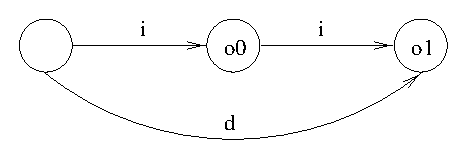
\includegraphics{figures/callfsaeg.eps}}
\centerfigend{fig-callfsaeg}{Sample FSA to Place Integer and Double 
	Floating Point Arguments on Registers}

Given the inadequacy of CCL for out task, we have developed two
new specification languages to support our analysis. The first,
IPL\footnote{\it Keep those acronyms coming!!} (instruction
pattern language) supports the specification of the instruction
sequences from which the caller and callee prologues and epilogues
are composed. IPL is an extension of SLED~\cite{Rams94b}, a language
to support descriptions of machine instruction syntax. IPL extends
SLED to provide support for regular expressions to the language where
the atoms of an expression are individual instructions. The second
language we have developed is PAL (procedure abstraction language).
which provides a means for specifying the calling convention and
other procedure aspects of object code as specified in an ABI.

The following sections demonstrate the use of these
specification languages for the SPARC and Intel platforms. More
detailed descriptions of the languages are given in the \uqbt\ 
source code. 


\section*{SPARC}

The standard stack frame for a single SPARC procedure is composed
of (from low to high addresses) a 16-word area to save the register
window, one word to put the address of a struct/union to return by a
callee, 6 words for a callee to save the first 6 arguments (passed
in registers) to the stack, $n$ words for output arguments 7 and
above, and an area to store locals.  Figure~\ref{fig-stkfrmSparc}
shows the standard stack frame for SPARC.

\centerfigbegin
\resizebox{8cm}{!}{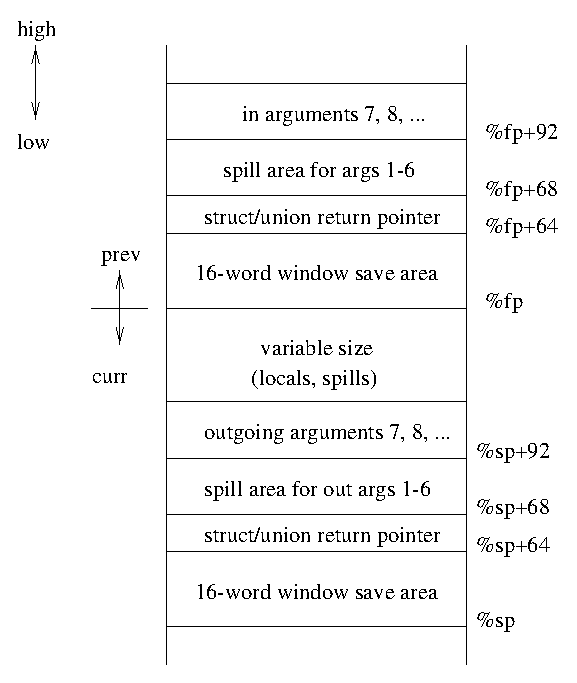
\includegraphics{figures/stkfrm-sparc.eps}}
\centerfigend{fig-stkfrmSparc}{Standard Stack Frame for SPARC Code.
The indexes and register's are given from the context of the callee.}


\subsection{Prologues and Epilogues}

Prior to specifying the prologues and epilogues, it is convenient
to introduce symbolic names for register encodings\footnote{This
is analogous to the {\tt names} construct in SLED.}. For example,
the symbolic name for register 24 on SPARC is {\tt \%o0}. The
set of names defined for SPARC are shown below.

\begin{verbatim}
NAMES
    SP = 14
    FP = 30
    o0 = 8
    i0 = 24
    i7 = 31
    o7 = 15
    g0 = 0
\end{verbatim}

On the SPARC, there are two different ways of invoking a function
based on the return type of the function.  A \texttt{call}
instruction is always used. If the return value is a structure,
union or a quad floating point value, the instruction following the
delayed instruction of the \texttt{call} needs to be a \texttt{unimp}
instruction.  The immediate 22 bits of the \texttt{unimp} are used
to specify the size of the returned value\footnote{Not all compilers
(e.g. gcc) make use of this information to generate runtime size
checking code.}.

\begin{verbatim}
PATTERNS
    CALLER_PROLOGUE std_call addr IS
        call__ (addr)

    CALLER_PROLOGUE struct_call addr IS
        call__ (addr); 
        <4>;  # any 4 byte instruction
        UNIMP (imm22)
\end{verbatim}

The callee prologues that have been identified to date are shown
below. The first two are used when the size of the stack to be
allocated fits into a 13 bit immediate operand. The first one effects
a change to the register window (i.e. allocates a new set of {\it
local} and {\it out} registers) where as the second doesn't. The last
two are analogs of the first two and handle procedures that allocate
a stack whose size cannot be stored in a 13 bit number. A procedure
may not have a prologue at all, as in the case of a leaf procedure
(see page 198 of~\cite{Sparc8}) that doesn't require any stack space.

{\it Note: The last two patterns shown here cannot be used yet as
the pattern parser cannot handle equations or local variables. See
\S\ref{sec:future_work} for a complete description of what is yet
to be implemented to support procedure recovery.}

\begin{verbatim}
    CALLEE_PROLOGUE new_reg_win locals IS
        SAVE ($SP, imode(locals), $SP)

    CALLEE_PROLOGUE same_reg_win locals IS
        ADD ($SP, imode(locals), $SP)

    CALLEE_PROLOGUE new_reg_win_large locals { locals = hiVal+lowVal } IS
        sethi(hiVal,reg);
        ADD (reg, imode(lowVal), reg);
        SAVE ($SP, rmode(reg), $SP)

    CALLEE_PROLOGUE same_reg_win_large locals { locals = hiVal+lowVal } IS
        sethi(hiVal,reg);
        ADD (reg, imode(lowVal), reg);
        SAVE ($SP, rmode(reg), $SP)
\end{verbatim}

The callee epilogue for a procedure on SPARC depends on the following
factors:

\begin{itemize}
\item Does it return an aggregate value?
\item Is it a leaf procedure?
\item Is the value to be returned (if any) already in the right
      location?
\item Has it allocated its own stack?
\end{itemize}

While most combinations of these factors are legal, the majority
of programs will only use a limited subset of the possibile
combinations.  The most common represents a standard return from
a non-leaf procedure (and hence resets the register window). The
value to be returned is already in the expected location ({\tt \%o0}
in this case). The alternatives for the first instruction (i.e. the
actual transfer of control) represent the cases of a scalar (or void)
return value and an aggregate return value respectively.

\begin{verbatim}
    CALLEE_EPILOGUE std_ret IS
        [ ret() |
          JMPL (dispA ($i7, 12), $g0) ];
        restore_()
\end{verbatim}

Two other common combinations are similar to the above except the
value to be returned is moved into the expected location by the
{\tt restore} instruction.

\begin{verbatim}
    CALLEE_EPILOGUE ret_reg_val rs1, rs2 IS
        [ ret() |
          JMPL (dispA ($i7, 12), $g0) ];
        RESTORE (rs1, rmode(rs2), $o0)

    CALLEE_EPILOGUE ret_imm_val rs1, imm IS
        ret();
        RESTORE (rs1, imode(imm), $o0)
\end{verbatim}

Lastly, a leaf procedure usually returns with a {\tt retl}
instruction when returning a void or scalar value or a {\tt jmpl}
instruction when returning an aggregate value. The extra offset from
the calling address in the latter case is to skip the {\tt unimp}
instruction discussed previously.

\begin{verbatim}
    CALLEE_EPILOGUE leaf_ret IS
        [ retl() |
          JMPL (dispA ($o7, 12), $g0) ];
        { SUB ($SP, imode(?), $SP) }
\end{verbatim}

Once the callee returns, any return values are in the right place
and the stack has been restored, so there is no caller epilogue.

The prologues and epilogues presented in this section are the basis
for the PAL specification. The PAL specification encapsulates the
information present in the ABI that describes how parameters are
passed and values returned, where locals are stored and any other
architecture specific information. The following sections present the
sections of the PAL specification for SPARC ABI compliant programs.

\subsection{Frame Abstraction}

To simplify a PAL specification, the first section specifies how to
abstract frame and stack relative address by converting them to be in
terms of a single fixed point, the abstract frame pointer (AFP or
{\tt \%afp}).  Typically, this point should be the value of the stack
pointer after the callee prologue (if any) has been effected as this
is when the abstraction specified takes place. On SPARC, {\tt \%afp}
is indeed initialised to the stack pointer (i.e. {\tt \%sp}). The
substitutions to convert other frame and stack relative addresses to
{\tt \%afp} relative addresses is specified in terms of the callee
prologues previously specified. The only two\footnote{Well four, if
you consider the prologues we can't yet handle.} callee prologues on
SPARC are similar enough that the same substitution for the frame
pointer (i.e. {\tt \%fp}) can be used.  The analysis tracks any
changes to either {\tt \%sp} or {\tt \%fp} throughout the procedure
and updates their respective substitutions correspondingly.

\begin{verbatim}
FRAME ABSTRACTION
    INIT = %sp
    new_reg_win
    same_reg_win
    {
        %fp -> %afp - locals
    }
\end{verbatim}


\subsection{Local Variables}
Local variables are stored within a procedure's stack frame. The size
of this stack frame can be derived from a callee prologue (\textit{We
are assuming that this is always true}). The example below states
that on SPARC, the amount of space (in bytes) allocated for local
variables is equal to the value of the {\tt locals} parameter of
the {\tt new\_reg\_win} and {\tt same\_reg\_win} callee epilogues.

\begin{verbatim}
LOCALS
    new_reg_win
    same_reg_win
    {
        locals
    }
\end{verbatim}

{\it Ideally, we would like to recognise any access addresses within
the portion of the stack frame used for local variables. However,
given the problem of aliasing this is non-trivial and requires
extensive analysis. Even with such analysis, there is no guarantee
that all such references will be detected. The approach we take is
simpler and completely reliable. The user specifies how to derive
the size of the block of memory allocated for locals from the callee
prologue\footnote{I am assuming that this will always be possible}.}

\subsection{Parameter Locations}

As discussed in \S\ref{sec-callConvSpec}, at the machine-code
level we cannot distinguish the variables and types that were used
when placing parameters on appropriate parameter-passing locations.
On SPARC, all parameters are copied by instances of one word, hence,
a double floating point value is copied as two words, in exactly
the same way as two individual integers or even two addresses are
copied.  Low-level type information can be retrieved from usage at
the called site.

The ABI specifies which locations are used for passing parameters,
and the order of usage of those locations. The means by which
the parameters are referenced across a call boundary is dependent
upon the {\it view change} effected by a call. The view change can
be thought of as the low level analog of using actual and formal
parameters in source code. That is, the same parameter is referenced
differently depending on whether the context of the reference is
the call instruction or in the called procedure.

To account for the view change effected by a call, we specify
parameter locations from the both context of the caller (outgoing
parameters) and the callee (incoming parameters).

The first part of the parameters section specifies where the outgoing
parameters are found. This is acheived by attaching a parameters
specification to the {\tt CALLER} keyword.

\begin{verbatim}
PARAMETERS
    CALLER
    {
        AGGREGATE -> m[%afp + 64]
        REGISTERS -> %o0 %o1 %o2 %o3 %o4 %o5
        STACK     -> BASE = [%afp + 92]
                     OFFSET = 4
    }
\end{verbatim}

Each sub-clause is optional but if present, it must obey the
ordering implied in the above example (i.e. {\tt AGGREGATE} before
{\tt REGISTERS} before {\tt STACK}). This ordering complies with
how parameters are passed on all architectures we have encountered.

The \texttt{AGGREGATE} sub-clause states where the address of an
aggregate value to be returned is found. This location will only
be used by calls to procedures that actually return a struct.
Additionally, only some architectures (such as SPARC) make use of
a special location for this purpose. Others (e.g. Intel) simply
pass it as the first parameter\footnote{This effectively makes it a
``hidden" argument in that it doesn't correspond to any source code
level parameter.}.

The {\tt REGISTERS} sub-clause states that registers {\tt \%o0..\%o5}
(in that order) are used for the first 6 parameters (after the
aggregate address parameter if used). Any extra parameters are
passed via the stack and are found in locations {\tt m[\%afp + 92],
m[\%afp + 96], m[\%afp + 100], ...} as specified by the {\tt STACK}
subclause.

In addition, there can be an {\tt ALIGNMENT} sub-clause, after the
{\tt STACK} and before the closing curly bracket. {\tt REGISTERS}
can also have a
type before it, to designate the type of parameters that the given
registers can hold. The type can be one of {\tt INTEGER}, {\tt FLOAT},
or {\tt DOUBLE}. Where a type is not given, as above, {\tt INTEGER} is
assumed. Where more than one type of register is given, they must be
in the order {\tt INTEGER}, {\tt FLOAT}, then {\tt DOUBLE} (with any or
all being optional). For example, for HP pa-risc:

\begin{verbatim}
PARAMETERS
    CALLER
    {
        AGGREGATE -> m[%r28]
        INTEGER REGISTERS -> %r26 %r25 %r24 %r23
        FLOAT   REGISTERS -> %fr4 %fr5 %fr6 %fr7
        DOUBLE  REGISTERS -> %fd5 %fd7
        STACK -> BASE = [%afp - 52]
                 OFFSET = -4
        DOUBLE ALIGNMENT 8 BYTES
    }

\end{verbatim}

When multiple {\tt REGISTERS} are given as above, they are considered to
operate ``in parallel". In other words, when the first parameter goes into
either \%r26 or \%fr4, this ``parameter slot" is ``used up", and so the next
parameter goes into register \%r25, \%fr5, or \%fd7, depending on the type.
If the first parameter is a {\tt DOUBLE}, then two parameter slots are
used up.

The {\tt ALIGNMENT} sub-clause states that parameters of type {\tt DOUBLE}
(64 bit floating point) are aligned on 8 byte boundaries. This applies to
registers and stack locations alike; that's why there are only two
{\tt DOUBLE REGISTERS}. As an example, if a pa-risc function took an
integer, a double, and an integer, then even though these could easily
fit into three registers, they are actually placed in registers \%r26,
\%fd7, and stack location [\%afp-52]. The alignment of the double parameter
``skips" register \%r25, and because doubles are twice as big as integers,
using \%fd7 ``uses up" the parameter slots for \%r24 and \%r23. So the third
parameter has to go to the stack. If there was a fourth parameter of type
{\tt DOUBLE}, it would go to [\%afp-64] (and the other half at [\%afp-60]),
skipping the word at [\%afp-56] to keep the argument aligned on 8 byte
boundaries.

This indicates a significant difference between SPARC and pa-risc architectures.
On the non aligned SPARC, a {\tt DOUBLE} parameter could be split between
an integer register and the stack. On the aligned pa-risc, such splits
can't happen. On the other hand, ``gaps'' in the parameters can be seen
in pa-risc programs, while these will never be seen on the SPARC.

Outgoing parameters are always placed at the same locations. Incoming
parameters however, depend upon the prologue of the procedure being
invoked as it is this prologue that effects the aforementioned
view change. Stack parameters may be found at different offsets
after allocation of the procedure's stack frame. Also, a register
window change will mean that some registers will now accessed via
different register names.

On SPARC, the {\tt new\_reg\_win} prologue changes the register
window, effectively renaming the eight output registers ({\tt
\%o0..\%o7}) to the eight input registers ({\tt \%i0..\%i7}).

\begin{verbatim}
    new_reg_win
    {
        AGGREGATE -> m[%afp - locals + 64]
        REGISTERS -> %i0 %i1 %i2 %i3 %i4 %i5
        STACK     -> BASE = [%afp - locals + 92] 
                     OFFSET = 4
    }
\end{verbatim}

The other prologue, {\tt same\_reg\_win}, doesn't change the register
window but changes the stack offsets.

\begin{verbatim}
	same_reg_win
    {
        AGGREGATE -> m[%afp - locals + 64]
        REGISTERS -> %o0 %o1 %o2 %o3 %o4 %o5
        STACK     -> BASE = [%afp - locals + 92] 
                     OFFSET = 4
    }
\end{verbatim}

\subsection{Return Locations}

Return values need to be placed in specific registers depending on
the type of the value to be returned. As with incoming parameters,
the locations used will depend on the view change effected by the
prologue of the procedure doing the return.

\begin{verbatim}
RETURNS
    ret_reg_val
    ret_imm_val
    leaf_ret
    CALLER
    {
        INTEGER   IN %o0
        ADDRESS   IN %o0
        FLOAT     IN %f0
        DOUBLE    IN %f0to1
    }
    std_ret
    {
        INTEGER   IN %i0
        ADDRESS   IN %i0
        FLOAT     IN %f0
        DOUBLE    IN %f0to1
    }
\end{verbatim}

Note that double refers to a 64 bit float and as such is returned in
a synthetic register that denotes two 32 bit registers.

Once again, the {\tt CALLER} keyword indicates that the accompanying
specification is from a caller's perspective. In this case it is
where a caller will receive a returned value.

\subsection{Accesses to a Parent's Stack}

This is the first (and so far, only) section that is optional in
that not all architectures will require it.

On SPARC, a procedure may write to a certain portion of its parent's
stack frame. This capability is provided primarily so that parameters
in registers can be spilled to the stack resulting in all parameters
being located in a contiguous segment of memory. This is typically
required when the source code uses variable argument lists or
takes the address of a parameter. Compiler writers can leverage
this capability and use this portion of the parent's stack as
space for temporary variables. In order to abstract away from
referring stack locations, we replace accesses to these addresses
with variables. To do so requires that these addresses are specified
in a PAL specification as shown below.

\begin{verbatim}
PARENT STACK
    new_reg_win
    same_reg_win
    {
        %afp - locals + 68 TO %afp - locals + 88 STEP 4
    }
\end{verbatim}

\section*{Intel}

The standard stack frame of a procedure includes space for arguments,
the return address of the caller, the frame pointer value of the
caller (\texttt{\%ebp}), and enough space for local variables and
spilled values (including registers that need to be preserved across
procedure calls).  Figure~\ref{fig-stkfrmIntel} shows the standard
stack frame for Intel code.

\centerfigbegin
\resizebox{10cm}{!}{\includegraphics{figures/stkfrm-intel.eps}}
\centerfigend{fig-stkfrmIntel}{Standard Stack Frame for Intel Code}

\subsection{Prologues and Epilogues}

As with SPARC, we start the prologue and epilogue specification by
declaring symbolic names for the register encodings.

\begin{verbatim}
NAMES
    EAX = 0
    ECX = 1
    EDX = 2
    EBX = 3
    ESP = 4
    EBP = 5
    ESI = 6
    EDI = 7
\end{verbatim}

On Intel x86, there is only one way to invoke a procedure, even if
the procedure is to return a value or a structure.  The \texttt{call}
instruction is used, and although this assembly instruction maps to
one of five different machine instructions, only one is used for
direct calls; the intra-segment direct call {\tt CALL\_.JVOD}.  For
indirect calls (i.e. via a register), the intra-segment indirect call
is used (CALL.EVOD modrm).  Indirect calls require extra analysis to
determine the target address of the call; this is addressed in a
different document.  For now assume all calls are direct.

\begin{verbatim}
PATTERNS
    CALLER_PROLOGUE std_call addr IS
        CALL.Jvod (addr)
\end{verbatim}

The most common callee prologue sets up the frame base pointer and
the stack pointer, as well as optionally allocating space on the
stack for locals and spilled values.  Further, the contents of
registers \texttt{\%edi}, \texttt{\%esi} and \texttt{\%ebx} need to
be preserved across procedure calls.  That is, if these registers are
used by the callee, they need to be spilled to the stack as part of
the prologue. 

\begin{verbatim}
    CALLEE_PROLOGUE std_entry locals=0, regs IS
        PUSHod ($EBP);
        MOVrmod ($EBP, Reg($ESP));
        { SUBiodb (Reg ($ESP), locals) |
          SUBid    (Reg ($ESP), locals) };
        { [ PUSHod ($ESI) |
            PUSHod ($EBX) |
            PUSHod ($EDI) ] *regs <1..3> }
\end{verbatim}

In the case where an aggregate value is to be returned, the address
at which this value is to be stored can be passed as the first
(hidden) argument of the call. It has been noted that some compilers
move this address into {\tt \%eax} as part of the prologue\footnote{
Initially this was believed to be an optimisation as the address of a
returned aggregate value must be in {\tt \%eax} upon returning from
the procedure.  However, analysis shows that this is not the case as
these procedures subsequently write to {\tt \%eax} before doing a
return. It does mean the simple form of {\tt RET} can be used in the
epilogue but I'm not sure that this can be classified as an
optimisation}.

\begin{verbatim}
    CALLEE_PROLOGUE struct_ptr locals, regs IS
        POPod ($EAX);
        XCHG.Ev.Gvod (E (Base ($ESP)), $EAX);
        @std_entry (locals, regs)  
\end{verbatim}

The standard epilogue restores any of the registers that need to be
preserved across a procedure call (i.e. \texttt{\%ebx},
\texttt{\%esi} or \texttt{\%edi}), restores the stack pointer and the
frame pointer, and returns to the caller's return address.  Restoring
registers to be preserved across procedure calls can be done in one
of two ways; by popping them from the stack, or by indexing into the
stack directly.  It has also been noticed that some compilers
generate a \texttt{LEAod} (load effective address) at the start of
the epilogue, to ensure the stack pointer is pointing to the right
address, even if this instruction is redundant (as has been seen in
gcc -O2 generated code). The {\tt RET.Iw} instruction is used to
remove the address of a returned aggregate value if this hasn't
already been done so by the prologue.

\begin{verbatim}
    CALLEE_EPILOGUE std_ret IS
        { LEAod ($ESP, Disp8(?,$EBP)) };
        { [ MOVrmod ($EBX, E( Disp8(?,$EBP))) |
            MOVrmod ($ESI, E( Disp8(?,$EBP))) |
            MOVrmod ($EDI, E( Disp8(?,$EBP))) ] * <1..3>
          |
          [ POPod ($EBX) |
            POPod ($ESI) |
            POPod ($EDI) ] *<1..3> };
        [ LEAVE () | [ MOVrmod ($ESP, Reg($EBP)); POPod ($EBP) ]];
        [ RET () | RET.Iw (?) ]
\end{verbatim}

Simple procedures that use no stack and take no parameters have a
very basic epilogue.

\begin{verbatim}
    CALLEE_EPILOGUE simple_ret IS
        RET () | RET.Iw (?)
\end{verbatim}
 

Upon return from a call, the stack needs to be restored by the caller in 
order to remove the parameters that were passed on the stack.  
Restoring of the stack is done by modifying the value of the stack
pointer by a certain number of bytes, or by popping values from the
stack a certain number of times (4 bytes at a time).  Either way 
will tell us how many bytes are restored from the stack. 

\begin{verbatim}
    CALLER_EPILOGUE clear_stack n IS
        [ ADDiodb (Reg($ESP),n) | ADDid (Reg($ESP),n) ] |
        [ POPod ($EAX) |
          POPod ($EBX) |
          POPod ($ECX) |
          POPod ($EDX) |
          POPod ($ESI) |
          POPod ($EDI) |
          POPod ($EBP) ] * n <1..7>
\end{verbatim}

\subsection{Frame Abstraction}

On Intel, we initialise {\tt \%afp} to be the value of {\tt \%esp}
after the prologue (if any) has been executed. As with SPARC, a
similiar substitution is specified for the frame pointer.

\begin{verbatim}
FRAME ABSTRACTION
    INIT = %esp
    std_entry
    struct_ptr
    {
        %ebp -> %afp + (regs * 4) + locals
    }
\end{verbatim}


\subsection{Local Variables}
The size of the block of memory allocated for local variables will
be the initial increment to the stack pointer plus the number of
bytes pushed to the stack when preserving registers.

\begin{verbatim}
LOCALS
    std_entry
    struct_ptr
   {
      locals + (regs * 4)
   }
\end{verbatim}

\subsection{Parameter Locations}

Outgoing parameters on Intel are always found at the bottom of the
stack. Given that we can't statically specify where the bottom of
the stack is, we simply choose a fixed stack address. Accompanied
with a negative offset, this implies that all address that are at
multiples of this offset from are potential parameter locations. The
analysis will then determine which of these locations are live at a
call and recovery as many as it needs to match the signature of the
callee, starting at the lowest addresses. This is exactly the same
approach taken with stack parameters on SPARC but the fixed point
specified in the SPARC PAL specification just happens to be the lowest
address (as implied by the positive offset accompanying it).

\begin{verbatim}
PARAMETERS
    CALLER
    {
        STACK     -> BASE = [%afp - 4]
                     OFFSET = -4
    }
\end{verbatim}

Procedures with the {\tt std\_entry} prologue will find their incoming
parameters at positive offset from the frame pointer. Of course, the
specification is given in terms of {\tt \%afp} as we want to abstract
away from concepts such as a frame pointer.

\begin{verbatim}
    std_entry
    {
        STACK     -> BASE = [%afp + locals + (regs * 4) + 8]
                     OFFSET = 4
    }
\end{verbatim}

The {\tt struct\_ptr} prologue contains the side effect of popping
the address of the aggregate value to be returned from the stack into
{\tt \%eax}\footnote{It it turns out that some other register is used,
then the register used can be parameterised in the pattern and the
parameter name used here instead of {\tt \%eax}.}. As such, the
incoming parameters specification for procedures prefixed with this
prologue require an {\tt AGGREGATE} location to be included.

\begin{verbatim}
    struct_ptr
    {
        AGGREGATE -> %eax
        STACK     -> BASE = [%afp + locals + (regs * 4) + 8]
                     OFFSET = 4
    }
\end{verbatim}

\subsection{Return Locations}

The RETURNS section specifies where returned values can be found. Again,
there are subsections for each callee prologue, and one for callers, using
the special keyword CALLER. Often the different integer values (byte,
short, int) are returned in the same register. If, and only if, the register
numbers are different for the integral subtypes, then an entry should exist
for INTEGER.16 and so on. On a RISC machine like SPARC, parts of registers
are typically not given different register numbers, so these don't appear:

\begin{verbatim}
RETURNS
# Note: even though functions with save/restore return integer locations in %i0,
# we use the STD_RET_ pseudo instruction for these, which copies %i0 to %o0.
# This simulates the semantics of the restore (for the purposes of return
# location), so we don't need a separate set of locations for these functions
    ret_reg_val
    ret_imm_val
    leaf_ret
    std_ret
    CALLER
    {
        INTEGER.32  IN %o0
        ADDRESS     IN %o0
        FLOAT.32    IN %f0
        FLOAT.64    IN %f0to1
    }
\end{verbatim}

On Intel, all fixed point scalar values are returned in {\tt \%eax},
but the word and byte part of eax is called a different register name.
All floating point values are returned on the top of the floating
point stack. The register number of the top of stack depends on whether
a caller or callee is involved:

\begin{verbatim}
RETURNS
    std_ret
    frameless_epi
    {
        INTEGER.32  IN %eax
        INTEGER.16  IN %ax      # So that functions returning shorts
        INTEGER.8   IN %al      # or chars can be analysed as such
        ADDRESS     IN %eax
        FLOAT.80    IN %st7
    }

    CALLER
    {
        INTEGER.32  IN %eax
        INTEGER.16  IN %ax      # So that functions returning shorts
        INTEGER.8   IN %al      # or chars can be analysed as such
        ADDRESS     IN %eax
        FLOAT.80    IN %st
    }
\end{verbatim}

\subsection{Accesses to a Parent's Stack}

Intel procedures never access any stack locations outside of their
own stack apart from those storing incoming parameters.

\section{Procedure Abstraction Analysis}

The goal of this analysis is to use the specification described in the
preceeding sections to remove any references to stack locations in
object code. Such references will be recovered into either parameters
or local variables. There are 5 steps involved in this analysis:

\begin{enumerate}
\item Replace all stack and frame pointer relative addresses with
  their equivalent {\tt \%afp} relative addresses.
\item Recover the signature (parameters only) of user code procedures.
\item Analyse each call to recover the actual parameters of the call.
  this step also includes recovering the return type of the procedure
  called if it isn't a library procedure.
\item Replace any accesses from within a procedure to locations in its
  parent's stack with accesses to local variables.
\end{enumerate}

This analysis is to be performed only on user procedures; library
procedures will be assumed to have been processed by now, either
through generation of call signatures from header files or through
application of the following analysis to library code.

The following subsection consider each of the above steps in
detail. Throughout this section we will make use of the SPARC
example in Figure~\ref{fig-c_gcd}.  Issues specific to Intel are
discussed in $\S$\ref{sec-callsigIntel}.

\centerfigbegin
{\small
\begin{verbatim}
gcd:                           main:
    save %sp,-112,%sp               save %sp,-112,%sp
    mov %i0,%l0                     mov 10,%o0
    cmp %l0,%i1                     mov 5,%o1
    bge .LL12                       sethi %hi(.LLC0),%l0
    mov %i1,%i0                     call gcd  
    b .LL12                         or %l0,%lo(.LLC0),%l0
    mov %l0,%i0                     mov %o0,%o3
.LL6:                               mov %l0,%o0
    call .rem                       mov 10,%o1
    mov %i0,%o1                     call printf  
    cmp %o0,0                       mov 5,%o2
    bne,a .LL12                     ret
    add %i0,-1,%i0                  restore
    mov %i1,%o0
    call .rem  
    mov %i0,%o1
    cmp %o0,0
    be .LL10
    nop
    add %i0,-1,%i0
.LL12:
    cmp %i0,1
    bg .LL6
    mov %l0,%o0
.LL10:
    ret
    restore
.LLC0:
    "gcd of %d, %d is %d\n"
\end{verbatim}
}
\centerfigend{fig-c_gcd}{SPARC Assembly Code for GCD Program}


\subsection{Recovery of Parameters}
Actual parameters are placed by the caller in one or more of the
locations specified by \texttt{caller parameters}.  The callee
will effect the \texttt{view change} applicable to its prologue, 
and will then use the passed parameters directly or place them 
on the parameter spill area.  Either way, the parameters are 
used before definition within the callee, and this is what 
tells us that the information in that location was setup elsewhere
in the program. 

In the example of Figure~\ref{fig-c_gcd}, \texttt{main} calls 
\texttt{gcd}, using the most frequently used calling convention;  
\texttt{interface1}.  
At the \texttt{call} site, the parameter locations that are live are: 
\begin{verbatim}
     live = {%o0, %o1}
\end{verbatim}
At the callee site, we apply the \texttt{view change} of 
\texttt{callee\_prologue1} to the live parameter locations, the 
stack pointer, and the return address, leading to
\begin{verbatim}
     %o0 -> %i0
     %o1 -> %i1
     %sp -> %fp
     %o7 -> %i7
     %sp -> %sp-112
\end{verbatim}
For \texttt{gcd} we summarize the live-in information for the whole 
procedure based on the parameter locations (view changed).  This gives us
\begin{verbatim}
     liveIn(gcd) = {%i0, %i1}
\end{verbatim}
This information tells us that there are 2 parameters, which match the
two live parameter locations at the call site, hence the actual 
parameters to the call are \texttt{\%o0} and \texttt{\%o1}.  The 
transformed CALL instruction looks like this:
\begin{verbatim}
     CALL gcd [<ret type>] <(%o0,<type>), (%o1,<type>)>
\end{verbatim}

Note that for parameter locations that are on the stack, the 
view change of these looks as follows:
\begin{verbatim}
     %sp+92+n -> %fp+92+n
\end{verbatim}
Hence, accesses to \texttt{\%fp+92+n} at the callee site are 
accesses to parameter locations.  It is also feasible for the
callee site to access these locations using the stack pointer; 
this is needed for leaf routines but it can also be used in 
non-leaf routines: 
\begin{verbatim}
     %sp+(92+simm13)+n
\end{verbatim}
We need to support both views of stack parameter locations.


\subsubsection*{Fixed vs Variable Number of Arguments}
Most procedures take a fixed number of arguments.  However, languages
like C allow for variable number of arguments to be passed at any
one time.  The ABI~\cite{Unix90} does not place any rules on variable 
number of parameters, but states that the calling convention rules need to 
be satisfied; that is, the first 6 word parameters go into registers
and the next go onto the stack.  Disassembled C code shows that 
the first thing the callee does is to move all the register parameters
to the parameter spill area, and then use them all on the stack 
(as the stack parameters are contiguous to the spilled register 
parameters). 

It is not clear that in all cases usage analysis of parameter 
locations at the callee will determine the number of parameters
taken by the callee (think of \texttt{printf}, it can take any
number and the code is bound to be a loop on a string).  
Also, different invocations of the procedure will take different
number of arguments.
\emph{I propose we pass all the live parameter locations at the call
site in the mean time; we will see from the implementation whether
this will cause problems with stack parameter locations.}


\subsection{Recovery of Return Value}
The callee will place a return value on a valid \texttt{callee return}
location.  We note that if anything is placed on a return location,
this location will be live-out of the callee.  
The caller will need to apply the inverse of the \texttt{view change}
to live-out callee locations.  
If the caller is to make any use of a returned value, the location
where it was stored will be used before being re-defined.  Usage is 
commonly in the form of storing to a local variable or using it
as a parameter to another procedure.  
Once this is determined, the callee's RET instruction is set to 
return the relevant return location.
 
For the example of Figure~\ref{fig-c_gcd}, the callee, \texttt{gcd}, 
has only one return location live-out, which matches its \texttt{callee
return} for \texttt{interface1}: 
\begin{verbatim}
     live-out = {%i0}
\end{verbatim}
The caller uses \texttt{\%o0} before definition, hence this is our
return location. 
The callee's RET instruction can now be transformed to: 
\begin{verbatim}
    RET %i0
\end{verbatim}
The caller's CALL instruction can now be transformed into an ASSIGN 
(assignment) instruction as follows: 
\begin{verbatim}
    %o0 = CALL gcd <(%o0,<type>), (%o1,<type>)>
\end{verbatim}

\emph{Should we introduce a HL ASSIGN or shall we use RTL assign 
instead?}

Note that as of 8th September 2000, the return value analysis is done before
the actual parameter analysis. This is because the return value analysis
may cause re-analysis of some of the children, which may impact on the
parameters of the call being considered.

\subsubsection*{Returned Values not Used}
Returned function values are not always used by the caller.  In such
cases, different invocations of the same procedure will show different
return location usage.  In these cases, we go for the more general 
one (i.e. the procedure returns a value) and we annotate each actual 
call with whether the return value is used or not.  In this way, the
signature for the procedure is correct. 


\subsection{Issues Relating to Intel Call Signature Analysis}
\label{sec-callsigIntel}
The nature of Intel passing parameters on the stack means that
optimizing compilers may delay the restoring of the stack until 
after several calls to (different) procedures have been emitted. 
This means that the caller epilogue is optional, and where 
available, it may not necessarily match the number of bytes 
passed as parameters to the caller but may also include bytes
used in a previous call.  We can still make use of liveness 
analysis to determine which arguments are passed to each procedure 
nevertheless.
For the purposes of illustration, we will make use of 
Figure~\ref{fig-gcdIntel}, an optimized version of the GCD program for Intel.

\centerfigbegin
{\small
\begin{verbatim}
gcd:                        main:
    pushl %ebp                  pushl %ebp
    movl %esp,%ebp              movl %esp,%ebp
    pushl %edi                  pushl %esi
    pushl %esi                  pushl %ebx
    pushl %ebx                  movl $10,%esi
    movl 8(%ebp),%ebx           movl $5,%ebx
    movl 12(%ebp),%edi          pushl %ebx
    movl %edi,%esi              pushl %esi
    cmpl %edi,%ebx              call gcd
    jge .L12                    pushl %eax
    movl %ebx,%edi              pushl %ebx
    jmp .L12                    pushl %esi
.L6:                            pushl $.LC0
    movl %ebx,%eax              call printf
    cltd                        leal -8(%ebp),%esp
    idivl %edi                  popl %ebx
    testl %edx,%edx             popl %esi
    jne .L7                     leave
    movl %esi,%eax              ret
    cltd
    idivl %edi
    testl %edx,%edx
    je .L13
.L7:
    decl %edi
.L12:
    cmpl $1,%edi
    jg .L6
.L13:
    movl %edi,%eax
    leal -12(%ebp),%esp
    popl %ebx
    popl %esi
    popl %edi
    leave
    ret  
.LC0:
    "gcd of %d, %d is %d\n"
\end{verbatim}
}
\centerfigend{fig-gcdIntel}{Intel Optimized Assembly Code for GCD Program}

Procedure \texttt{main} calls \texttt{gcd} using the calling convention 
specified in \texttt{interface2} with an immediate value of 12 bytes. 
The calling convention does not include a caller epilogue. 
At the \texttt{call} site, the \emph{parameter locations} that are live are: 
\begin{verbatim}
     live = {[%esp], [%esp+4]}
\end{verbatim}
Applying the \texttt{view change} for \texttt{interface2} to the live
parameter locations we get: 
\begin{verbatim}
     ['%esp]   -> [%esp+20]
     ['%esp+4] -> [%esp+24]
and
     ['%esp]   -> [%ebp+8]
     ['%esp+4] -> [%ebp+12]
\end{verbatim}
Procedure \texttt{gcd} has the following set of parameter locations
live on entry, and return locations live on exit: 
\begin{verbatim}
     liveIn = {[%ebp+8], [%ebp+12]}
     liveOut = {%eax}
\end{verbatim}
The liveIn parameters match the ones that were live on entry, hence 
we can safely assume that 2 words (8 bytes) were passed as arguments.
The call is transformed to the following HL instruction: 
\begin{verbatim}
    CALL gcd [<ret type>] <([%esp],<type>), ([%esp+4],<type>)>
\end{verbatim}
which is further transformed into what was actually placed at those 
stack locations (i.e. this information needs to be stored previously): 
\begin{verbatim}
    CALL gcd [<ret type>] <(%esi,<type>), (%ebx,<type>)>
\end{verbatim}
The liveOut information tells us that \texttt{\%eax} is returned. 
Further, at the caller's site, the value of \texttt{\%eax} is 
used prior to definition.  Even if this value was not used, the ABI 
states that return locations should only be set to a value if they
are intended to return a value, as there is no type checking on 
this interface.  The return instruction in \texttt{gcd} is changed to
\begin{verbatim}
     RET %eax
\end{verbatim}
and the caller's site call is changed to 
\begin{verbatim}
     %eax = CALL gcd <(%esi,<type>), (%ebx,<type>)>
\end{verbatim} 
Although there is no caller epilogue to restore the stack, we have
determined the right arguments to this call.

The next call that \texttt{main} performs is to the library procedure 
\texttt{printf}.  In this case, if we had signatures for \texttt{printf} 
we could only be assured of one fixed parameter (an address) and maybe
some more parameters, as this is a variable argument procedure.  
Also, the calling convention does not specify a caller epilogue in 
this case either, hence we cannot determine exactly how many bytes
are passed on the stack to this call.  The best that can be done is
to pass \emph{all} parameter locations that are live at the call site: 
\begin{verbatim}
     live = {[%esp], [%esp+4], [%esp+8], [%esp+12], [%esp+16], [%esp+20]}
\end{verbatim} 
When replacing this information into the HL call, we get: 
\begin{verbatim}
     CALL printf <(.LC0,<addr>), (%esi,<type>), (%ebx,<type>), (%eax,<type>),
                  (%esi,<type>), (%ebx,<type>)>
\end{verbatim}
Note that in this case, the last two arguments are still technically
live as the stack wasn't restored.  Although we are passing them to 
\texttt{printf}, the code within \texttt{printf} will not use them 
as they were not expected (by checking the string \texttt{.LC0}). 

If however the stack was restored after the call to \texttt{printf}, 
the following code could have been emitted to restore both calls made
by \texttt{main}: 
\begin{verbatim}
     addl $24, %esp
\end{verbatim}
Which would account for 8 bytes that we already know \texttt{gcd} takes
as arguments, and 16 bytes for \texttt{printf}.  This type of arithmetics
will allow us to determine the number of bytes passed to variable 
argument procedures in some cases (bearing in mind that each time 
a different number of arguments may be passed). 


\section{EBNF for the PAL Language}

The EBNF for the PAL language follows.  The standard EBNF
metasymbols are used:

\begin{itemize}
\item \verb!{a b}! for sequence
\item \texttt{[a]} for optional constructs
\item \texttt{(a|b)} for alternative choices
\item \texttt{*} for zero or more occurrences
\item \texttt{+} for one or more occurrences
\end{itemize}

\begin{fnverbatim}
PALSpec ::= register_names
      caller_prologue_section callee_prologue_section
      callee_epilogue_section [ caller_epilogue_section ]
      frame_section local_section parameter_section
      return_section [ parent_section ]

register_names ::= "NAMES" { name '=' number } +

caller_prologue_section ::=
      "CALLER_PROLOGUE" pro_epi_decl +
callee_prologue_section ::=
      "CALLEE_PROLOGUE" pro_epi_decl +
callee_epilogue_section ::=
      "CALLEE_EPILOGUE" pro_epi_decl +
caller_epilogue_section ::=
      "CALLER_EPILOGUE" pro_epi_decl +
pro_epi_decl ::= constructor_list

frame_section ::= "FRAME ABSTRACTION" init_decl
      frame_decl +
init_decl ::= "INIT" reg_name
frame_decl ::= name + '{' reg_name "->" afp_exp '}'

local_section ::= "LOCALS" local_decl +
local_decl ::= names '{' exp '}'

parameter_section ::= "PARAMETERS" param_decl+
param_decl ::= names
      '{' "AGGREGATE ->" "m[" afp_exp ']'
          "REGISTERS ->" reg_name +
          "STACK -> BASE = [" afp_exp ']'
                   "OFFSET =" number '}'

return_section ::= "RETURNS" return_decl +
return_decl ::= names
      '{' "INTEGER IN " reg_name
          "ADDRESS IN" reg_name
          "FLOAT IN" reg_name
          "DOUBLE IN" reg_name '}'

parent_section ::= "PARENT STACK" parent_decl
parent_decl ::= name + '{' afp_exp "TO" afp_exp
      "STEP" number '}'

operands ::= name { "," name } *
constructor ::= name { '(' operands ')' }
constructor_list ::= constructor
      | constructor ';' constructor_list
exp ::= "(" exp ")"
      | exp "+" exp | exp "-" exp
      | exp "*" exp | exp "/" exp
      | reg_id | number | name
afp_exp ::=
      "%afp +" exp | "%afp -" exp
reg_name ::= name | reg_id

names  ::= ( name | "CALLER" ) +
name   ::= [A-Z][A-Z0-9_]*[A-Z0-9]
number ::= [0-9]*
reg_id ::= '%'[A-Za-z][A-Za-z0-9]*
\end{fnverbatim}


\section{Location Sets}

Many of the analyses described in this chapter rely on sets of bits representing
locations. This section gives an overview of the LocationMap and BitSet classes
which implement these.

\subsection{LocationMap class}

There is one LocationMap object (part of the CSR class) for the whole program.
It represents a mapping from the integers to locations of interest to the
translation. For example, in one translation, integer 0 might represent "r[8]",
and in another translation it could represent "m[\%afp+92]". It is convenient
to define sets of bits to represent sets of locations. In these sets, if
but {\it n} is on, that means that the expression represented by integer {\it n}
is in the set. That way, expressions such as

  $live_{in}~ = ~\stackrel{\bigcup}{_{all BBs}} ~UsedUndefined~ \bigcap
  ~~({\rm U} - live_{in}$)

can be implemented in code such as

    {\tt for (}{\it bb = each in-edge}{\tt )} \\
    \indent {\tt liveIn |= bb->useUndefSet \& \~~(bb->liveIn);}

\subsection{BitSet class}

There is a Standard Template Library (STL) template class called
\texttt{bitset}, which implements a fixed-size array of bits. Unfortunately,
since we don't know in advance how many locations a program may have, we want a
class with the same functionality as \texttt{bitset}, but has a variable size
(like a vector of bits).  The \texttt{BitSet} class implements this
functionality, using a \texttt{vector} of unsigned integers to hold 32 bits
at a time. Standard bitwise operators like \& and $|$ are used to implement
set intersection and union respectively.

Objects of class \texttt{BitSet} have a member variable called \texttt{usedBits}
which stores the number of bits in this set.
Bits are numbered from 0 to \texttt{usedBits-1}.
\texttt{BitSet}s sometimes have to represent the universal set.
To do this properly, there is a boolean class member called \texttt{universal},
which represents the bits numbered from \texttt{usedBits} to infinity.
Normally, \texttt{universal} is zero, so that the set is finite, and bits
not stored in the vector are considered zero. However, the member function
\texttt{set()} (the one taking no arguments) sets the single vector element
to all ones, and sets the \texttt{universal} bit as well. All bits of this
set are considered to be one.

It is important to take the \texttt{universal} bit into consideration when
performing operations such as \texttt{operator\&}, \texttt{set({\it n})},
and so on. Two member functions, both with the name \texttt{setUsed},
expand the vector when required (e.g. setting or clearing a bit higher than can
be represented with the vector at its current size, or \texttt{and}ing or
\texttt{or}ing with a bitset larger than can be represented with the vector
at its current size. When the vector is expanded, the newly inserted words
are either set to all zeroes or all ones, depending on the state of the
\texttt{universal} bit.

Extra care must be taken when \texttt{and}ing or
\texttt{or}ing with a set smaller (in terms of vector size) than the current
set. For example, when \texttt{and}ing with a smaller set, those elements of
the vector beyond the size of other operand's vector are effectively being
\texttt{and}ed with a virtual word whose bits are all set to the other
operand's \texttt{universal} bit. Hence these words are cleared if the other
operand's \texttt{universal} bit is zero, or left the same otherwise.


\section{Future Work for Procedure Abstraction Recovery}
\label{sec:future_work}

This section details possible extensions and enhancements that can be
made to the procedural abstraction module within UQBT (Doug, Sep 99).

\subsection{Pattern Language for Prologues and Epilogues}

The proposals in this section include extensions to the pattern
language itself (IPL), improvements to the corresponding parser
and suggestions to enforce constraints on how the patterns are used.

\begin{itemize}
\item Add support for locals. Locals are variables that are not
  parameters and as such don't require definition before use. Locals
  can be used to constrain operands over a number of instructions
  without requiring that a parameter is used. Also can be used in
  equations. The example below from SPARC displays both uses:

\begin{verbatim}
    CALLEE_PROLOGUE new_reg_win_large locals { locals = hiVal+lowVal } IS
        sethi(hiVal,reg);
        ADD (reg, imode(lowVal), reg);
        SAVE ($SP, rmode(reg), $SP)
\end{verbatim}

  In this example, {\tt hiVal}, {\tt lowVal} and {\tt reg} are
  all local variables. The first two are used in the equation
  to set the value of the {\tt locals} parameter. The {\tt reg}
  variable enforces the operands of the same name in each of the
  three instructions to have exactly the same value for the whole
  pattern to be successfully matched.

\item Add support for equations. This enables pattern definitions
  like the one above where the value of an operand is derived from an
  expression involving operands of the constituent instructions. In
  this form, equations are exactly the same as supported by SLED.
  However it may be desirable to given equations a finer grained
  scope than the whole instruction. This would allow pattern
  definitions such as the one below where the value of a parameter
  is derived or explicit depending on which branch of the matching
  expression was taken.

\begin{verbatim}
    CALLEE_PROLOGUE new_reg_win locals IS
        SAVE ($SP, imode(locals), $SP) |
        [ sethi(hiVal,reg);
          ADD (reg, imode(lowVal), reg);
          SAVE ($SP, rmode(reg), $SP)
          { locals = hiVal + lowVal }
        ]
\end{verbatim}

  The primary advantage of this extension is that one epilogue
  can match a greater variety of patterns. However it comes at
  the disadvantage of added complex to both the language and the
  underlying parser. As it is, the parser will have to extend its
  semantic checking for equations to ensure for example that any
  variables used in the right hand side of an assignment are defined
  on every branch of the matching expression (e.g. lowVal and hiVal)

\end{itemize}


\subsection{Local Variables}
The current local variable section in a PAL spec only supports
specification of the size of the stack frame which in turn is
the amount of memory we allocate for local variables. On some
architectures such as SPARC, the stack frame includes space for
other purposes than just storing local variables such as space
for saving the register window in the case of a register window
overflow. We would like to be able to allow the user to
specify the portion of the stack frame that is dedicated to local
variables. One means of doing so is to specify a base address and a
size (similar to a stack parameter specification) as in the following
example for SPARC:

\begin{verbatim}
    LOCALS
        new_reg_win
        same_reg_win
        {
                BASE = %afp
                SIZE = locals
        }
\end{verbatim}

This example says that the locals parameters are located in the
inclusive range {\tt m[\%afp] .. m[\%afp + locals]}. Using such a
specification ensures that the translated program will only allocate
as much space for locals as was allocated in the source program.

{\it As long as only the size of the stack is specified, the local will
always be indexed at offsets from {\tt \%afp}. For this reason, the
size specified must always be the same as the difference between the
frame pointer and its equivalent {\tt \%afp} relative value. This can
be seen to hold in both the SPARC and Intel PAL specs.}


\subsection{Aggregate Types as Parameter and Return Types}
When analysing calls to user code procedures, both the caller
and callee can be coerced into a form that will guarantee the
successful compilation of the generated intermediate C code on
the target platform. This results primarily from the fact that the
underlying exposes the calling convention for passing and return
aggregate values in the intermediate code.

Library procedures that have aggregate types in their signature will
expect the calling convention on the target platform for passing
and returning these types to be used by calls to them. The only
way we can do this in C code is to typecast the blocks of memory
storing the relevant aggregate values. Consider a call to the
library function with the following signature:

\begin{verbatim}
    time_t time(time_t *t);
\end{verbatim}

To ensure that the code generated by a call to this function
will be ABI compliant with the library on the target platform, the
intermediate C code must use the {\tt time\_t} name as follows:

\begin{verbatim}
    (*(time_t*)(_t) = time(_t);
\end{verbatim}

where {\tt \_t} is a pointer to the block of memory that will store
the {\tt time\_t} struct. There is no need to typecast the parameter
to the call as type clashes between pointer types will result in
compiler warnings but the correct code will be generated. A typecast 
would have been necessary for the parameter if it was not a pointer type.

At the moment, the analysis does not have access to the type names
required for doing the typecasting described above.

\subsection{Implementation}

This sections describes what is left to be done in the implementation
is general apart from the changes suggested in the preceeding
sections.

\begin{itemize}
\item Change all "csr" substring "pal" to reflect that CSR module is
now the PAL module. This includes changes to directory names, files
names, class names, variables name comments etc.
\end{itemize}

         % procedure abstraction recovery

 	%
% 25 Oct 01 - Brian: Added description of endianness analysis during
%              type analysis.
%

\chapter{Type Recovery Analysis}
\label{ch-type}

\newtheorem{typerule}{Type Rule}[chapter]

{\small
\begin{flushright}
Design: Cristina [Mar 99], Implementation: Mike Van Emmerik[c.00], Bernard Wong [Aug 01], Documentation: Cristina [99], Bernard [Aug 01], Brian [Oct 01]
\end{flushright}
}

{\em The bulk of this document was written in 1999 and has not 
been updated much since.  In summer 2001, Bernard implemented some 
of the type propagation ideas presented in this chapter, 
however, the implementation is not fully tested at the 
time of release of this code.} 

Low-level type recovery is the process of recoverying types 
that are available at the machine level in order for 
translated programs to be correct.  
Type recovery is done in a series of steps, by first annotating
locations with their plausible type and then propagating 
types across live ranges of locations.  

This document will grow as we learn more about the type 
requirements for translated programs.  The following are 
the issues that will be addressed throughout this process: 
\begin{itemize}
\item What is the minimal set of low-level types required?
\item How do we best propagate information across procedures?
\item What information do we need to store for byte swapping 
	to work correctly across different endianness machines?
\end{itemize}

In reality, we are mainly interested in determining the low-level 
types for parameters and return values, however, in order to 
do that, one needs to also know the types for other locations 
that define the variables that get passed as parameters. 
This analysis will be done in the following stages: 
\begin{itemize}
\item Recovery of types for registers
\item Recovery of types for local and parameter locations that 
	are not registers 
\item Recovery of types for other memory locations
\end{itemize}

The second stage involves extending the register analysis to 
support local variable locations as well as parameter locations. 
It may be that parameter locations are trivially supported by
the register analysis (once parameters have been determined), 
and so this stage would be involved with the support of 
local procedure memory.

The last stage is an optional one and is there in case we end 
up doing endianness analysis and attempt to minimize the number
of swaps to memory.  

Unless otherwise seen to be needed later, we will work with 
four base low-level types: integer, float, address to data 
and address to instruction.  
Given that the ABI~\cite{Unix90} states that floats and 
integers (of any size) are passed on integer registers, and the  
fact that addresses are also integer numbers, our default data type
for any location is an integer (i.e. the bottom of the lattice).  
In a lattice representation, if a condition holds true, a type can 
be promoted to one higher up the lattice.  In our case, we have a 
few types which can be represented in a very simple lattice as per 
Figure~\ref{fig-typeLattice}. 

\centerfigbegin
%\resizebox{6cm}{!}
{\includegraphics{figures/typeLattice.eps}}
\centerfigend{fig-typeLattice}{Lattice of Low-Level Types} 

Types are determined based on usage of a location across a live
range.  Given that a particular location can be re-used as 
different variables of different types by a compiler, the only
safe assumption is that the live range for a given location will 
have \emph{one} type.  {\emph{I believe this assumption is 
valid for non-overlapping registers.}} 

For the promotion of types, we use a slightly different lattice
to the one displayed in Figure~\ref{fig-typeLattice}.  Distinguishing
integers from addresses is a hard to solve problem as the assembly 
of the machine does not provide for mnemonic instructions to 
distinguish them.  For example, the following code: 
\begin{verbatim}
    sethi %hi(71167),%o1
    or %o1,%lo(71167),%o0
\end{verbatim}
sets register \texttt{\%o0} to the value of \texttt{71167}.  From 
looking at this code alone we cannot tell whether 71167 represents
an address (in the instruction or data area) or a large constant 
number.  Only usage of register \texttt{\%o0} will determine 
the type of 71167.  
For this reason we use the lattice in Figure~\ref{fig-promotionLattice} 
to describe the types of addresses; namely, an integer may ``look like'' 
and address, but until we can identify usage of that integer or 
address, we cannot determine whether it is an address (and hence 
promote to type address). 

\centerfigbegin
\resizebox{6cm}{!}{\includegraphics{figures/promotionLattice.eps}}
\centerfigend{fig-promotionLattice}{Lattice of Low-Level Types}

Once a type is determined, types are propagated across the live range 
of the particular location.

Note that even though we place data at the same memory locations
in the target address space as in the source address space, we 
still need to collect type information on pointers to data, as 
this information is needed in getting byte swapping (i.e. the 
simple endianness solution) to work correctly on translated 
programs.


\section{Type Analysis for Registers}
By default, a register is considered to be an integer 
register.  Usage of a register on a procedure call or 
as the return value of a call can change its type.  
Types are propagated from usage to definitions, so here are 
the steps to follow at different parts of the translation 
process: 

\begin{itemize}
\item Collect plausible type information at decoding time.
\item Perform type propagation by type induction.
\end{itemize}


\subsection{Collecting Type Information at Decode Time}
There are three rules that can be used at decoding time 
to annotate type information in registers.  

The first two rules deal with static checking of literal 
constants against addresses of text and data sections, and 
annotating the relevant register to ``looks like'' an address, 
denoted, ``\verb!~!pi'' for looks like a pointer to an instruction, 
and ``\verb!~!pd'' for looks like a pointer to data.  

\begin{typerule}
If a M$_S$-RTL instruction is of the form ``r = Num'' and 
$Num \in$ addrRanges(textSegments), then type(r) = \verb!~!pi.
\label{rule-llpi}
\end{typerule}

\begin{typerule}
If a M$_S$-RTL instruction is of the form ``r = Num'' and 
$Num \in$ addrRanges(dataSegments), then type(r) = \verb!~!pd.
\label{rule-llpd}
\end{typerule}

The following rule applies to any control transfer instruction, 
namely, calls, conditional and unconditional jumps. 
If the target address of the control transfer instruction is 
stored in a register, than that register has pointer to 
instruction type, denoted ``pi''. 

\begin{typerule}
If an M$_S$-RTL instruction is of the form ``controlTransfer r'', then 
type(r) = pi. 
\label{rule-pi}
\end{typerule}


\subsection{Determining Live Ranges of Registers}
In order to propagate types across registers and across 
procedures, live ranges for each register need to be found
first.  A register may take several different variables 
throughout the lifetime of a procedure, hence the need for 
such live ranges. 

A live range extends between the definition (i.e. assignment)
of a register until the death (i.e. re-assignment) of that register.
For example, in the following \texttt{main} code:
\begin{verbatim}
2    mov 10,%o0
3    mov 5,%o1
4    sethi %hi(.LLC0),%l0
5    call gcd
6    or %l0,%lo(.LLC0),%l0
7    mov %o0,%o3
8    mov %l0,%o0
9    mov 10,%o1
10   call printf
11   mov 5,%o2
12   ret
\end{verbatim}

The live ranges for register \texttt{\%o0} are: 
\begin{itemize}
\item Register \texttt{\%o0} becomes live at instruction 2,
    and its live range extends to instruction 5
\item instructions 5 to 8
\item instructions 8 to 10
\item instructions 10 to 12
\end{itemize}


\subsection{Propagating Type Information}
Type propagation can only be performed in \hrtl\ code, i.e. 
after parameter analysis recovery has been performed and 
the program's code has been lifted to the level of machine 
independent RTLs. 

Known types (i.e. non integer) are propagated across live 
ranges of registers, including across procedure calls, 
taking into consideration the signatures for library 
functions.

The first rule states how to go up the lattice when the type 
of the RHS is non integer, basically, propagate from the type of 
the usage to the type of the definition.

\begin{typerule}
If a \hrtl\ instruction is of the form ``r = exp'' and type(exp) = A 
and type(r) = int, then type(r) = A. 
\label{rule-prop-usageDef}
\end{typerule}
 
Note that the type of an expression is the type further up the
lattice of the individual registers forming the expression. 

The next rule looks at the return value of a function call 
and propagates that type to the newly defined register. 

\begin{typerule}
If a \hrtl\ instruction is of the form ``r = call X'' and 
returnType(X) = A, then type(r) = A. 
\label{rule-prop-retValue}
\end{typerule}

The next rule states that a library function's formal argument 
types are propagated to the associated actual parameters.  
In the case of variable argument functions, only the fixed 
formal parameter types can be propagated. 

\begin{typerule}
If a \hrtl\ instruction is of the form ``call libFunc(..., $r_i$, ...)'' 
and the function libFunc has the signature ``libFunc(..., $f_i$=$t_i$, ...), 
then type($r_i$) = $t_i$.  
\label{rule-prop-libFunc}
\end{typerule}
 
The above three rules can be applied on a pass through the code, 
without need of any extra data structures other than the live 
ranges for registers.  The next rule requires extra analysis to 
be performed on procedures, as a register that appears as 
pointing to an instruction may actually be invoked elsewhere in
the program, such as in the \texttt{qsort} program.  

\begin{typerule}
If there is an instruction of the form ``call r''and $\exists$ r2: 
type(r2) = \verb!~! pi, then, if r2 \ra* r, type(r2) = pi. 
\label{rule-reach}
\end{typerule}

In order to apply type rule~\ref{rule-reach}, we need to compute
the reaching definitions of $r2$ throughout the program, including
its transitive closure as the register could have been passed 
as parameter and then copied to another register before it is 
invoked. 


\section{Type Analysis for Other Memory Locations}
Type analysis of other memory locations
can be done to support endianness analysis:
the identification of when endianness swaps are necessary
when the target machine has a different endianness than the source machine.
A translated program's initialized memory is left as-is,
in the source machine's endianness.
We currently swap the bytes of \emph{every} multibyte value
that is read or written to memory.
If type analysis were extended
to include information about the endianness of each value,
then we could determine not only which endianness swaps are unnecessary,
but also when they must \emph{not} be done.
For example, the procedure \texttt{scanf}
is passed an address where its result must be stored.
The value that will be stored in memory
will be in native (target) endianness.
However, when the caller reads the value,
if its bytes are swapped, the native value will be corrupted.
This problem occurs today with every ``call-by-reference'' procedure
that takes addresses where their results are written.

We could do a data flow analysis to discover what values
have native endianness and what do not.
This could be done during type analysis
and a bit set indicating the endianness of each value and location.

Note that it is not enough to specify ``call-by-reference'' information
for just library procedures such as \texttt{scanf}.
The translated program's own procedures
may also be ``call-by-reference''. 


\section{Speculative Decoding}
Trees of program code can be built through speculative 
decoding, in such a way that a forest of trees is built, 
with the main tree being the one that starts at the 
program's entry point.  
Speculative decoding is useful if code ever gets code 
through the interpreter, in which case, the interpreter's 
switch manager can determine if the target address has
already been decoded, in which case, efficient translated
code is run instead of being interpreted.  However, 
speculative decoding is expensive on time resources, 
but for static translators this may be ok anyway.  
 
Type rule~\ref{rule-prologue} states that for all word-aligned
values of $N$ that belong to any of the text segments, if 
the first bytes of that address match a callee prologue (see  
Chapter~\ref{ch-call}, \S\ref{sec-callConvSpec} for SPARC and Pentium 
callee prologues), then $N$ is the start address of a new 
code tree.  

\begin{typerule}
$\forall N: N$ is word-aligned and $N \in addrRanges(textSegments)$ 
and $m[N] \ldots m[N+i]$ = callee\_prologue then type($L$) = $pi$.
\label{rule-prologue}
\end{typerule}

Clearly, applying this technique would be done after the 
normal decoding process and \uqbt\ should have tagged which 
word-aligned memory locations have already been processed 
so that those locations are ignored in this lengthy pass. 


\iffalse
\section{Promotion to Address to Data}
Addresses to data point to data locations in the program, such as
constant data (for example, strings that appeared in the original 
program), and global read and write data. 

An address is an integral number that happens to be a virtual address 
within the range of addresses of the data segment(s) of the program or of 
a symbolic name. 
In Elf binary-files, there are several sections that contain data; 
these are: 
\begin{itemize}
\item Sections that contain read-only data: .rodata, .rodata1
\item Sections that contain initialized read-write data: .data, .data1
\item Section of uninitialized read-write data: .bss
\end{itemize}
Each of these sections has identifying information to know the 
section name, its virtual address and its size.
This data provides us with information that can be used in 
determining whether an integer is an address to data or not. 

The following rules are used to promote integers to addresses to data.
We denote ``address to data'' by $addr_d$ and ``looks like address to 
data'' as $ll_{addr_d}$. 

\begin{typerule}
If $m[i]$ then type(i) = $addr_d$
\label{rule-index}
\end{typerule}

Type rule \ref{rule-index} states that any memory access implies an address 
through its index.  This will be the case for both load and store 
instructions.  Further, $i$ may be an expression, in which case 
the registers within it will contain the value of the address. 
For example:
\begin{verbatim}
  %o0 = m[%l0+4] 
\end{verbatim}
implies that \texttt{\%o0+4} is an address, in which case 
\texttt{\%o0} is the register that contains the address.  

\begin{typerule}
If $L_1 = a[L_2]$ then type($L_1) = addr_d$.
\label{rule-addressOf}
\end{typerule}

Type rule \ref{rule-addressOf} states that if the address of a location is 
taken, then the location represents an address to data.  For example,
the following two RTLs illustrate this point:
\begin{verbatim}
  r[24] = a[m[0x804a250]]
  r[24] = a[m[r[29]-8]]
\end{verbatim}

\begin{typerule}
If $L = Num$ and $Num \in$ addrRange(dataSegments) then type($Num) = ll_addr_d$ 
and type($L) = ll_{addr_d}$.
\label{rule-dataSeg}
\end{typerule}

Type rule \ref{rule-dataSeg} states that if an integral constant is within 
the range of the virtual addresses of the data segment(s) of a program (i.e. 
.rodata, .rodata1, .data, .data1 or .bss in an Elf binary-file), then 
both the integral constant and the location to which it is assigned 
looks like an address to data.  

\emph{Is the information in the dynamic symbol table for type STT\_OBJECT 
relevant?  It contains the virtual address of such objects.}

As can be seen, the type rules that promote to address to data cannot
always solve the problem of accessing data addresses.  However, in 
our implementation, we \emph{force} the data segment(s) of the source 
binary program to be located at the same virtual addresses in the
target program.  Hence, determining whether an address points to 
data or not, does not need to be solved using this model; and 
type rules~\ref{rule-index} to \ref{rule-dataSeg} are not used. 


\section{Promotion to Address to Instruction}
An instruction address points to instructions in a program, normally
the start of procedures or entry points into the code of a function. 

An address to an instruction is a virtual address that falls 
within the text section(s) of the program.  For Elf binaries, the
following sections contain instructions: 
\begin{itemize}
\item The program's text section: .text
\item The program's initialization section: .init
\item The program's finalization section: .fini
\item The program's program linkage table: .plt
\end{itemize}
Further, the dynamic symbol table (.dynsym) also contains names of 
dynamic library procedures.  Such names map addresses which are 
found in the PLT section.

The following rules are used to promote integers to addresses to 
instructions.  We denote ``address to instruction'' by $addr_i$ 
and ``looks like an address to instruction'' by $ll_{addr_i}$.

\begin{typerule}
If $Call L$ then type($L$) = $addr_i$.
\label{rule-call}
\end{typerule}

Type rule \ref{rule-call} states that if a call is made to a target 
location, then that location represents an address to an instruction. 
This rule covers both, calls to known addresses and otherwise, 
such as in the following examples: 
\begin{verbatim}
  call 0x10ae4        ; known target address
  call r[10]          ; computed call, unknown statically unless analyzed
\end{verbatim}

\begin{typerule}
If $Jump L$ then type($L$) = $addr_i$.
\label{rule-jump}
\end{typerule}

Type rule \ref{rule-jump} states that the target location of an 
unconditional jump points to an instruction.

\begin{typerule}
If $Jcond L$ then type($L$) = $addr_i$.
\label{rule-jcond}
\end{typerule}

Type rule \ref{rule-jcond} states that the target location of a 
conditional jump is an address to an instruction.

\begin{typerule}
If $L = Num$ and $num \in$ addrRange(textSegments) then 
type($Num$) = $ll_{addr_i}$ and type($L$) = $ll_{addr_i}$.
\label{rule-textSeg}
\end{typerule}

Type rule \ref{rule-textSeg} states that an integral constant looks 
like an address to an instruction if that constant is within the
range of virtual addresses of the text sections of the program. 
In the case of Elf binary-files, the text sections are .text, 
.init, .fini and .plt. 

\begin{typerule}
If type($L$) = $ll_{addr_i}$ and $L$ uniquely reaches $r[i]$ in 
a $Call r[i]$ statement, then type($L$) = $addr_i$.
\label{rule-reach2}
\end{typerule}

Type rule \ref{rule-reach2} states that a reaching definition of a 
location that looks like an address to an instruction is in fact
an address to an instruction, if the statement it reaches is a 
computed call on a register.

\begin{typerule}
If type($L$) = $ll_{addr_i}$ and $m[L] \ldots m[L+n]$ = callee\_prologue
then type($L$) = $addr_i$.
\label{rule-prologue}
\end{typerule}

Type rule \ref{rule-prologue} states that an integral constant that 
looks like an address to instructions can be promoted to an 
address to instruction if the bytes at that memory location and subsequent 
locations match those of a valid callee prologue (see 
\S\ref{sec-callConvSpec} for SPARC and Pentium callee prologues).

Type rule \ref{rule-prologue} creates a forest of code that is decoded
statically, even when the caller of such code cannot be determined
statically.  In the event of dynamic invocation of such code, 
if the code has been translated, the interpreter's switch manager
will check the address translation table and determine that such
code has already been translated, hence giving control to it 
instead of interpreting it. 

By the nature of building the control flow graph while decoding 
machine instructions, we are in essence applying type rules~\ref{rule-call} 
to \ref{rule-jcond}.  

Type rules~\ref{rule-textSeg} promotes a type to ``looks like an 
address''.  If neither type rules~\ref{rule-reach2} or~\ref{rule-prologue} 
applies, then we cannot say that the particular integral constant is an 
address or not.  As it \emph{may} be an address, we will need to 
pass it as an address in order to prevent programs from crashing. 
In the event that it was an integral constant instead of an address, 
we will emit the wrong result.  

\emph{Can we somehow trap this?  If it goes to a library function,
we have the signature in most cases (except varargs), if it goes 
to user code, then we would have translated it, so we could check 
prior to invoking?}
 

\section{Promotion to Float Type}
A float type is determined when placing a location onto a 
floating point register.  Type conversion procedures such as 
\texttt{itof()}, integer to float, not only perform a type 
conversion but also set the live range of the source and 
target registers used; the source register dies and the target
register starts its live range.  The size of a float is determined
based on the usage of the floating point register(s).  For 
example, when a double register is used, then its size is twice 
the word size (64 for SPARC). 

There are two different types of float values, those that are 
constant and those that go into registers.  The constant values
are easy to determine from the RTLs, as a float number is 
represented by \texttt{FloatNum} in the EBNF and an integer 
number as \texttt{Num}.  

Floating point registers are separate to integer registers in our
RTL model, hence any values that pass through floating point 
registers are of type float.  Further, floating point operators 
and procedures (such as sin and cos) also aid in determining how a 
particular register is used.  

The following rules determine the values of type float: 

\begin{typerule}
If $V = FloatNum$ then type(V) = float.
\label{rule-float}
\end{typerule}

Type rule~\ref{rule-float} states that if a value is of the 
RTL type FloatNum, then it is a floating point value.

\begin{typerule}
If $L = FFunction$ then type(L) = float.
\label{rule-floatFunc}
\end{typerule}

Type rule~\ref{rule-floatFunc} states that if a function that
returns a float is used, then the type of the location becomes
a float.
Note that this rule implies that a register may be used to 
hold integer and floating point values at different points in 
time in the program, hence the live range for a register needs 
to be considered carefully. 

\begin{typerule}
If $L = (Exp BinOP Exp)$ and $BinOP \in Farith$ then type(L) = float.
\label{rule-floatOp}
\end{typerule}

Type rule~\ref{rule-floatOp} states that if a floating point arithmetic
operand is used on the right-hand side expression being assigned to 
location $L$, then the result type of the expression is a float and
hence $L$ is of type float.

\fi


\section{Register Live Ranges}
In order to perform some of the promotion analysis, we need to 
keep track of live ranges for all registers used in a procedure. 
The importance of this is that a register may hold values of 
different types at different points in the program, hence we 
cannot just say ``register 5 is of type float'' as it may be
that it is of type integer and then becomes of type float.  
\emph{A suitable data structure to keep track of ranges and 
types is needed.}

\emph{The following example should be on the RTLs rather than
the assembly code, but uqbts is giving the wrong answer}

A live range extends between the definition (i.e. assignment) 
to a register until the dead (i.e. re-assignment) of that register. 
For example, in the following \texttt{main} code from Figure~\ref{fig-c_gcd}: 
\begin{verbatim}
2    mov 10,%o0
3    mov 5,%o1
4    sethi %hi(.LLC0),%l0
5    call gcd  
6    or %l0,%lo(.LLC0),%l0
7    mov %o0,%o3
8    mov %l0,%o0
9    mov 10,%o1
10   call printf  
11   mov 5,%o2
12   ret
\end{verbatim}

By the time the analysis is done, we will have performed the 
prologue/epilogue analysis, hence the first and last instructions 
are not there.  The live ranges for register \texttt{\%o0} are: 
\begin{itemize}
\item Register \texttt{\%o0} becomes live at instruction 2, 
	and its live range extends to instruction 5 
\item instructions 5 to 8 
\item instructions 8 to 10
\item instructions 10 to 12
\end{itemize}


\section{Reaching Definitions}
In order to apply type rule~\ref{rule-reach}, we need to compute 
the reaching definitions of $L$, the transitive closure of 
reaching definitions.  The use of the \texttt{qsort} example 
is ideal in this case, as two levels of indirection are needed 
in order to find the location where a function pointer gets used. 


\section{Type Recovery Analysis Implementation}

{\small
\begin{flushright}
Implementation and documentation: Bernard [Aug 01]
\end{flushright}
}

In order to evaluate the type recovery processes discussed in the previous
sections of this paper, an initial implementation of type recovery
analysis based on this paper has been completed.

This implementation however is only an initial version and does not
implement every rule stated in this paper. The following is a list of 
type rules that the current version of type recovery analysis implements:

\begin{itemize}
\item Type Rule~\ref{rule-pi} "controlTransfer r", then type(r) = pi
\item Type Rule~\ref{rule-prop-usageDef} "r = exp" and type(exp) = A and 
	type(r) = int, then type(r) = A
\item Type Rule~\ref{rule-prop-retValue} "r = call X" and returnType(X) = A 
	then type(r) = A
\item Type Rule~\ref{rule-prop-libFunc} Type propagation between library 
	functions
\end{itemize}

Without rules~\ref{rule-llpi} and \ref{rule-llpd}, it is not possible to 
implement the ``looks like'' types mentioned earlier in this paper.  
Therefore, the different low-level types that are represented are integer, 
address to instruction, address to data and float.

The first necessary step is to infer the plausible type information of each 
register in each of its live ranges. This step is done after the binary
files has been brought up to the HRTL level of abstraction. It is possible
to perform the initial type recover at the machine specific RTL level. However,
important information such as parameters and return value to functions are not 
available at the machine specific RTL level and will need to be added later. 
For simplicity of implementation reason, it was decided that the type recovery 
analysis will begin after the binary file has been bought up to the HRTL level.

The first information that we want to gather from the HRTL is the location
of every use and definition of each register. From this information, we
can build use-definition chains and determine the live ranges of each register.
Since we assume that the type information for a non-overlapping register in a 
particular live range is always the same, therefore each use-definition chain 
would only have one type and can be used as a means to propagate type 
information of each register across instructions. The use-definition chain 
is therefore one of the most important data structure we use for type recover.

To actually infer the type information, the HRTL instructions need to be parsed
for specific cases that uncover the type information. The HRTL instructions are 
stored in a prefix format as a list of integers called semantic strings. The 
simplicity of this prefix format allowed the creation of a parser, specific
to uncovering type information from semantic strings, to be a relatively 
straight forward process. The following is a list of some of the cases
which the parser is looking for:

\begin{itemize}
\item Registers within MemOf tokens. This can be complicated by functions
	and operations following MemOf tokens.
\item Registers following a control transfer token. 
\item Certain binary operator that has implict type information to the registers
	it operates on.
\item Certain function operators, which often has explict type information
	to the registers it operates on.
\end{itemize}

The parser will first find all the registers that are in the semantic string and
determine whether it is a use or definition of the register. It will insert
this information into a use-definition chain data structure. The parser will
also insert into the data structure any type information that it can infer.

Additional, the parser will look for simple register aliasing situations that 
can later be used for type propagation. For example, in the following example, 
register 1 and register 2 are consider aliases in type value. The 
use-definition chains of these two register at this particular point will be 
linked together. Therefore, if more type information was later discovered 
about register 2, the type information of register 1 would also be updated.

\begin{verbatim}
r[1] = r[2]
\end{verbatim}

This stage of type recovery will already uncover a significant amount of type
information. Long use-definition chains will likely have the correct type
information as the many uses of the register would most likely uncover the
type. 

In order to find the complete use-definition chains for every register, the
program must be analyzed in its entireity. Each register must be tracked 
from its first definition to its last use. There are several implementation
problems with tracking a register in that manner. One problem is the difficulty
in tracking a register as the flow of instruction passes a control transfer
instruction. A register can be defined before the control transfer instruction 
and then be used in both the branches. Therefore, the data structure used for 
the use-definition chains must be complex enough to handle this case correctly.
A second problem is the size of the data-structure used to hold the 
use-definition chains. Since the backend of UQBT that performs code generation 
only looks at HRTL code a basic block at a time, it would be much more 
convenient to also have use-definition data structures for each basic block 
instead of a monolithic one for the whole program. 

The approached that was taken in this implemenation was to create use-definition
chains at the basic block level. This was chosen mostly because of its 
simplicity.  The use-definition chains will always be straight lines at the 
basic block level, as there will not be any control transfer instructions. 
Retrieving the information to insert into the data-structure is also a simple 
process as all the information can be found inside each basic block. 
Therefore, the code to generate the data structure is small and modularized 
for different types of basic blocks. However, the main disadvantage to creating
the use-definition chains at the basic block level is that the chains are 
often incomplete. Many chains will only have uses but no definitions and some 
chains will only have definitions but no uses.
Therefore, this data structure does not store the equivalent amount of 
information as the one that covers the complete program. However, the missing 
information can be recovered by performing type propagation across basic 
blocks and across functions.
The type propagation is simply completing incomplete chains across basic 
blocks and functions. 

To implement type propagation across basic blocks, a depth first traversal of 
the basic blocks inside each function is performed. During the depth first 
traversal, a pointer to the parent of each basic block is kept inside the 
basic block's data structure. At each basic block, use-definitions chains that 
have uses but no definitions are found and are made candidates for type 
propagation. Determining which chains are candidates is a very quick task as 
there are only certain places where incomplete chains may be. Incomplete 
chains are always found as the first use-definition chain of each register.
And each chain can only have one definition which, if it exists, is always 
the first element in the chain. Therefore, only $n$ elements needs to be looked 
at for each basic block to determine which chains need to be propagate, where 
$n$ is the number of registers. Next, to find the definition part of the 
chains, the algorthm will traverse up the call graph, using the pointer to 
the parent basic block stored during the traversal. 

Since this traversal follows the flow of normal execution, traversing back up 
the control flow graph should always find the desired register definition. 
However, there are cases where this might not be true because of the 
limitation of keeping only one single pointer to the parent basic block. It 
also depends on the aggressiveness of the traversal.

The original traversal algorithm that was implemented would only consider every
basic block once. Once a particular basic block has been reached, a flag is 
marked to indicate that future traversals should end before reaching this basic
block. However, this traversal is much too conservative as it only consider one
path to each basic block when there could possibly be many paths. To solve this 
problem, a more aggressive traversal algorithm allowed a basic block to be 
traversed multipled times. To avoid infinite loops, it still marks basic blocks
that have been traversed. When a basic block that has been traversed is reached,
it would be traversed again but be treated as a leaf node. Therefore, the 
algorithm would not continue to traverse down this path any further and avoid 
possible infinite loops. However, this still introduces a possible infinite 
loop situation when dealing with back branches due to the limitation of 
keeping only one pointer to the parent's basic block. 

\begin{verbatim}
   A
   |
   B      Assume the straight path from B to C is going down
   |\     and the crooked path from B to C is goind up (back branch)
   |/
   C
\end{verbatim}   
	  
Suppose that register 1 is defined in basic block A and used in basic block 
B. To traverse this graph, the path A-B-C would be taken. Once basic
block C has been reached, it would try to traverse to basic block B. Since
basic block B has already been traversed before, its traversal flag will 
be set. However, with the second algorithm, it would still be traversed
again and treated as a leaf. 

When basic block B is reached for the second time, it is discovered that
it contains a use-definition chain with uses but no defines for register 1.
Backwards traversal of the graph using the parent pointer would be used to
find the basic block with the definition of register 1. However, the parent
pointer of basic block B now points to basic block C, and the parent pointer
to basic block C points to basic block B. Therefore, this traversal will never
complete as the definition of register 1 is in basic block A.

To work around this possible problem, the implemented algorithm will try to 
detect any loops in the traversal. In most cases, this is enough to overcome 
this problem. However, there still exist cases where infinite loops can occur. 
A maximum number of basic block traversal was added to work around these 
special cases.

Propagating type information across functions is done in a very similar way as
propagating across basic blocks. The complexity of propagating across functions
is slightly higher as every call site and every return site in each function
must be recorded. With propagation of return value, it could involve a large set
of registers as a function can have many return sites which would all involve
different use-definitions chains of registers. This is actually benefitual to
the type propagation as it implies that the whole set of registers must all 
be the same type.

Type propagation may seem to be even more complicated and complex than simply
creating complete use-definition chains. However, the beauty of type 
propagation is the ability to propagate type information from library 
functions. Since the type information for parameters and return value for 
standard C functions are known, any call to these functions will allow 
trusted type information to be propagated back to user functions.


\subsection{Results}
The following type information was inferred for the function \texttt{myCompare}
which can be found in the \texttt{qsort2} regression program:

\begin{verbatim}
Currently In Procedure: myCompare
Registers stored in this Basic Block are:
8       --> Def @ 108c8    -->  <32pd>  Use @ 108cc 99
                                        Contains Alias
        --> Def @ 108cc    -->  <32i>   <no_use>
9       --> Def @ 108cc    -->  <32pd>  Use @ 108cc 99
                                        Contains Alias
24      --> Def @ param    -->  <32pd>  Use @ 108c8 0
                                        Contains Alias
25      --> Def @ param    -->  <32pd>  Use @ 108cc 0
                                        Contains Alias
\end{verbatim}

The above data output shows that we were able to identify that register 8 was
defined at address 108c8 and used at address 108cc. It also identified that
the register is of pointer to data type at those two instructions. Registers 24
and 25 were also identifed to be pointers to data. The information about
registers 24 and 25 is especially important as both these registers are 
parameters to the myCompare function. Therefore, we now know what the type 
signature for the myCompare function is. Also, all the register shown above
contain aliases. Therefore, if we found out any new type information about one
of these registers, the type information of at least another register would
also be updated.

This type information was manually checked against the HRTL instructions and 
also the original source code and was verified to be correct. However, no 
automated testing system to determine the type information correctness is 
currently available.


\subsection{Future work}
There are several areas which need to be worked on in order for more accurate
type recovery analysis in the future. Currently, although the type information 
for most registers are recovered, there still exist cases where the type 
information for a register is still not available. For these cases, 
rules~\ref{rule-llpi} and \ref{rule-llpd} can be used to determine possible 
type information. These possible type information may not be always correct 
but would allow the backend additional information to determine what the 
correct code that it needs to generate.

Type analysis should be extended
to determine the endianness of each value and location.
This is needed to know when it is incorrect to swap the bytes
of values loaded or stored to memory.
It will also allow us to avoid doing swaps that are unnecessary.

Backend support of the type analysis recover will also need to be added in the 
future. The information gathered through type analysis should significantly 
increase the correctness of the code generated by the backend.

Finally, a test suite that can automatically verify that the inferred type 
information is correct needs to be written. Currently, the only method of 
verification is manually analyzing every HRTL instruction by hand. An 
automated method that can use the orginal C source code to verify type 
information would be the ideal tool.

The current implementation has not been thoroughly tested, some 
propagation across procedures is not working as expected. 


         % type recovery analysis


\part{Backends}
\label{part-backends}

 	
\chapter{The C Back End}
\label{ch-cbackend}

{\small
\begin{flushright}
Design: Mike, Trent, Cristina. Implementation: Mike. 
Documentation: Mike [Nov 01], Cristina
\end{flushright}
}

We have experimented with different backends for \uqbt.  
In 1998 we started with an \rtl\ optimizer and chose VPO for 
this task.  VPO~\cite{Beni88} is a retargetable optimizer
of register transfers.  VPO's interfaces were clearly 
specified throughout 1998 as part of the Compiler 
Infrastructure Project~\cite{Vpo98}. This work is described 
in Section~\ref{sec-vpo}, which refers to work done in 
April 1998 and may no longer be current.  
We successfully interfaced to VPO and optimized 
SPARC-based programs.  However, the specs for Pentium
code were not available when we needed to test Pentium
based translations, so the focus changed to using off the shelf C
compilers as the UQBT optimiser. 
In 2001 we revisited the VPO backend and used it to optimize 
code for several target platforms, this work is described in 
Chapter~\ref{ch-vpobackend}.

The main optimizer that we have used throughout 1998-2001 has 
been via a C interface, i.e., we use a C compiler as an optimizer 
and generate low-level C code out of our \hrtl\ .
We have experimented with Sun's cc and GNU's gcc compilers 
and have obtained results with both on SPARC and Pentium 
platforms (see Chapter~\ref{ch-results} for 1999 results).  
The type of code that we generate is low-level 
C code, in that all control transfer is in the form of goto's,
it uses a lot of casting and is hard to read.  

The C backend makes extensive use of the \texttt{Translate} class. The main
reason for this is to prevent the need for passing around many parameters,
e.g. the stream (\texttt{os}), current procedure \texttt{proc}, and so on.


\section{The Current Type and Casting}

C operators are somewhat polymorphic. For example, the right shift operator
(\texttt{>>}) means either ``shift right arithmetic'' or ``shift right logical''
depending on the type of the operands (signed integer or unsigned integer
respectively). This contrasts with RTS, which uses different operators for
these two cases. The only way to ``tell'' the C compiler to perform one or the
other right shift operation is to cast the operands correctly. All integer
registers and variables are declared as signed, and are cast to unsigned as
needed. In general, it is necessary to be aware at all times of the
current type of an operand (which could be a primitive such as a register,
variable, or constant, or it could be a more complex expression), and
the type that the C compiler is going to assume that an operand is.
When these differ, a cast is required.

As an example, consider this simple assignment:
\begin{verbatim}
000125b8 *32* v0 := v0 >>A 24
\end{verbatim}

The right shift arithmetic operator can be specified in C by ensuring that the
first operand (\texttt{v0}) is unsigned. Since \texttt{v0} will be declared
as a signed integer, it will have to be cast.
The way that this works is that the expression
emitter (\texttt{Translate::processExpr}) (and many other back end functions)
take a parameter called \texttt{cType}, which is the ``current'' or
``expected'' type. For \texttt{idShiftR} and other ``unsigned'' operators,
the current type is forced to unsigned before being passed to
\texttt{processExpr}. (\texttt{idshiftR} is unusual in that it only requires
the first operand to be unsigned; other ``unsigned'' operators require
both operands to be unsigned). When \texttt{processExpr} recurses to process
the first operand (\texttt{v0}), it compares \texttt{cType} with the type
of \texttt{v0}, and finds a mismatch. A cast is therefore emitted.

There are two types of cast used in the backend. One is just a ``regular''
cast, e.g. \texttt{(unsigned)v0}. The other is referred to as a ``heavy
duty cast''; e.g. \texttt{*(unsigned int*)\&v0}. The latter can be understood
by reading it from right to left. We start with \texttt{v0}, of type ``int'',
then take its address, resulting in ``pointer to int''.
This is then cast to ``pointer to unsigned
int''; finally this is dereferenced to yield ``unsigned int''. The advantage
of the ``heavy duty cast'' is that it is possible to cast from almost anything
to almost anything else, e.g. \texttt{*(int*)\&f8} is of type \texttt{int},
even though f8 may be declared as type \texttt{float}. It is often important
to do this, because in changing types with a conventional cast, C will often
perform a \emph{conversion} operation. All conversions in RTL are explicit,
so the implicit conversion will usually result in unwanted semantics.

As an example, consider the translation of a Sparc \texttt{itof}
instruction. This instruction takes a bit pattern from a \emph{floating
point} register, interprets the pattern as an integer, converts it to a
floating point bit pattern, and writes this to the destination floating
point register. Let's say we are converting \%f2 to \%f3. Both \%f2 and
\%f3 are declared as floating point variables in the C output. To perform
the conversion, we need code like this:
\begin{verbatim}
  f3 = (float) *(int*)&f2;
\end{verbatim}
This code contains both a conventional (left) and a heavy duty (right) cast.
The heavy duty cast is needed to convince the C compiler to treat the bit
pattern in f2 as an integer. The conventional cast casues the conversion,
which in this case is the desired semantics. Note that the following would
not work:
\begin{verbatim}
  f3 = (float) (int)f2;
\end{verbatim}
The compiler would first convert f2 from float to integer, then back to float
again. The result is wrong, because the bit pattern in f2 is not in floating
point format to start with.

Note that heavy duty casts should not be used when there is a change of size
of the operand. Consider a big endian target machine, e.g. Sparc. Suppose that
r8 contains the value 5. Thus, \texttt{(int)r8} has the value 5, as expected.
However, \texttt{*(char*)\&r8} has the value 0! This is because the heavy
duty cast assumes that the address of a pointer does not change when the
object it points to changes. This is simply not valid for big endian
machines.

Semantic strings, which are used throughout UQBT to represent expressions,
have a single \texttt{Type} object, representing the type of the overall
expression. Whenever \texttt{SemStr::getSubExpr()} is called, the newly
created semantic string has the correct type for the subexpression. For
example, the overall type for the expression \texttt{itof(32, 64, r[24]}
is float64, but the subexpression (\texttt{r[24]}) is of type int32.
 

\section{Overlapping registers}

Many architectures have registers that have subsets that can be referenced
by name. For example, parts of the pentium register \texttt{\%eax} can be
referenced as \texttt{\%ax} (lower 16 bits), \texttt{\%al} (lower 8 bits),
and as \texttt{\%ah} (bits 8-15). UQBT has separate names for these register
parts, but obviously changing one register has to have the appropriate
effect on other registers. To complicate matters, the C representation for
these overlapped registers depends on the endianness of the source and target
machines.

Class \texttt{Overlap} (in \texttt{backend/common/overlap.cc}) handles these
complexities. It has methods to initialise itself (including the reading
of information from the \texttt{.ssl} file),
a method to record the use of registers, and methods for emitting C code
(both to declare the overlapping registers, and to emit code appropriate to
a particular register).

There is an extra pass through the procedure (\texttt{Translate::firstPass()})
whose main job is to find which registers are used by the procedure. This
information (kept in the instance member regNumbers, a set of integers) is
used to declare as a union only those overlapped registers that are needed
for this procedure. (Although there is little if any overhead in declaring
all possible overlaps, there would be very significant clutter in the output C
file).

For example, consider a pentium source program where register \texttt{\%eax}
(only) is accessed as both 32 bits and 8 bits. The 32 bit register happens
to be \texttt{r[24]}, and the 8 bit register happens to be \texttt{r[8]}.
The following C code declares these registers:
\begin{verbatim}
union {
        int32 i24;
        struct {
                int16 dummy1;
                int16 h0;
        } h;
        struct {
                int8 dummy2;
                int8 dummy3;
                int8 b12;
                int8 b8;
        } b;
} i24;
\end{verbatim}
When used as a 32 bit register, \texttt{\%eax} is referenced as
\texttt{i24.i24}. When used as 8 bits, it is referenced as
\texttt{i24.b.b8}. These locations can be assigned to, or used as values
in expressions.

Note that in this example, the target is a big endian machine (pentium is a
little endian machine). If the target was a little endian machine, the order
of the int16 and int8 elements in structs h and b would be reversed, to keep
h0 and b8 at the least significant end. This is automatically handled by
\texttt{class Overlap}.

The information needed by \texttt{class Overlap} is found in the \texttt{.ssl}
file. For example, in 80386.ssl, we see
\begin{verbatim}
[ %eax, %ecx, %edx, %ebx,
  %esp, %ebp, %esi, %edi ][32] -> 24..31,
%ax[16] -> 0 SHARES %eax@[0..15],
...
%al[8]  -> 8 SHARES %ax@[0..7],
...
%ah[8]  -> 12 SHARES %ax@[8..15],
...
\end{verbatim}


    % the C backend

	
\chapter{The JVML Back End}
\label{ch-jvm}

The Java Virtual Machine Language (JVML) back end was written as 
an experiment in translating machine code to run in a Java Virtual 
Machine (JVM).  There were 3 different versions of this back end. 
The original 1999 back end, \texttt{jbmu}, was a hand-written back end 
that supported translations of \hrtl\ onto JVML (i.e. Java bytecodes).
The \texttt{jbmu} translator was an experimental translator at best, 
to try and show the feasibility of translating to JVML.  The 
generated code would then be assembled by the Jasmin assembler. 
This translator is described in Section~\ref{sec-jbmu}. 

Realizing that so many of the optimizations that were needed in 
the \texttt{jbmu} translator were the same ones implemented by 
any optimizer such as the \texttt{gcc} compiler, Trent took over 
the job of writing a machine description (MD) file for the JVML 
language so that \texttt{gcc} could translated our low-level C 
code into JVML code, assembled by the Jasmin assembler. This 
work was done in 1999 and is described in Section~\ref{sec-gccjvm}.
The standalone \texttt{gcc} extensions to support JVML have been 
released under GPL and are not part of the distribution of the 
\uqbt\ system.  
 
In mid 2000, Sameer rewrote part of the JVML back end in Java, basically, 
making it similar in nature to the original \texttt{jbmu} back end.  
Brian extended this back end throughout the end of 2000, adding 
floating point support, non 32-bit integer types, type and size 
conversions, and more.  This translator is part of the 
\uqbt\ distribution, unfortunately, there is not much documentation 
for it at present time; we have put together some notes in 
Section~\ref{sec-jvmbackend}. 


\section{jbmu - A JVM Backend}
\label{sec-jbmu}

{\small
\begin{flushright}
Design: Trent and Cristina, Implementation: Trent, Documentation: Trent
[Mar 99]
\end{flushright}
}

This section describes the initial implementation of a JVM backend, 
jbmu, which was written in Java (Dec98-Feb99).  \uqbt 's intermediate 
representation was in fluctuation at the time, so the backend is 
dependent on an older version of \uqbt.  This backend was not completed; 
a second JVM backend was written for gcc.  
This documentation was written at a time when experimentation
with other stack-based languages was expected, as such, it
was designed to be retargetable.  
This chapter is left herein for historical reasons.  [Cristina - May 00]. 

The binary translation of an arbitrary source machine binary to stack
based machine bytecodes requires a generic frontend to produce non-machine
specific intermediate data and an efficient backend to produce target byte
codes.  To date, little work has been focused on the construction of
backends, especially for backends targeted at stack based machines.  
Current technologies in retargetable backends lend little to this task,
because they have taken the stance of Register Transfer Lists (RTLs) as an
intermediate representation.  This reduces the performance of target
machines that have less registers than source machines and fails to
address more serious needs of a stack based machine backend.  Other forms
of intermediate representation have been presented~\cite{Peyt99} but, to
date, RTLs appear the most recognised. The Java Virtual Machine, for
example, has no registers, however, the JVM specification allows any
method to use a defined number of local variables, which can be mapped
directly onto the integer registers of a source machine.  With these
problems in mind, we can state the task of the backend:

\begin{itemize}
\item To generate an internal representation.
\item To optimise that representation using non-machine specific
optimisations.
\item To perform generic stack based machine optimisations.
\item To generate bytecodes for a specific stack based machine.
\end{itemize}

The points above are well understood and their implementation can be seen
in compiler design but, despite this, there is little code that can be
reused in such a backend.  For this reason, it would be beneficial to
write a generic global optimiser that could be reused in other projects
and targeted at other machines.

\subsection{Non-Machine Specific Optimisations}

Non-machine specific optimisations can be done with no knowledge of the
target machine.  They are non-machine specific optimisations and, although
they sometimes can be improved with machine specific information, they are
generic and should be implemented with no knowledge of the target machine.  
This allows for the reuse of such code when retargeting to a different
machine.

The crucial stage of any backend is global optimisation.  Whatever the
internal representation, there is need for some basic optimisations:

\begin{itemize} 
\item Data flow analysis:  the movement of dead variable
values into sub-expressions.  This is particularly necessary in the case
of register-based machines to stack-based machines translation to
eliminate temporary register assignments.  This reduces the number of
``local variables'' a method requires which speeds up the overall code.

\item Constant folding:  any computation that can be done at compile time
is removed from the internal representation.  This leads to smaller
bytecode and less operations to be performed by the stack based
machine.

\item Common sub-expression elimination:  the availability of local
variables allows us to create temporaries for commonly used expressions.  
This prevents the re-computation of intensive expressions and reduces the
overall bytecode size.

\item Invariant movement and other optimisations:  more compiler
originated optimisations can be made by generating a control flow graph in
the internal representation and moving code.  This will result in faster
``inner loops'' and allow more opportunity for global optimisations like
constant folding. See~\cite{Aho86a} or~\cite{Fisc88b} for details.

\end{itemize}

\subsubsection{Bytecode Generation and Scheduling}

Every backend must eventually produce code for a specific target machine.  
This will inevitably lead to bytecode selection.  The instruction set of a
target machine may be redundant.  Often there is more than one way to
perform a series of operations with some being more efficent than others.
There are two primary solutions to this problem.  A compiler designer may
only use a subset of the available instructions, which leads to
inefficient code, or may attempt to choose the ``best'' instruction to
match the internal representation.

There is a lot of work on the subject and will not be
repeated here (for example, \cite{Emme88} speaks of a generic pattern
matching approach which may be useful, however, most of their code is in
Modula 2 and, as such, cannot be easily reused). Stack based machines
introduce more problems as the types of the operands must match the 
instruction generated.  This typing is to be considered extreme 
distinguishing between \texttt{char}, \texttt{int} and \texttt{byte} types.

The scheduling of instructions is most important on a stack-based machine.  
This can reduce the number of local variables used and, as a result, the
number of bytecodes need to store and retrieve them.  This is an obvious
job for dataflow analysis when the local variable is a temporary, but many
times the assignment of a local variable that is used at some later stage
can be replaced with an instruction that duplicates the value on the stack
at the appropriate moment.  These are topics that promise to give the most
optimisations in stack-based machine code.


\subsection{Internal Representations}

The retargetable stack based machine backend consists of a number of 
steps (figure ~\ref{fig-sbmbflow}):

\centerfigbegin
\resizebox{8cm}{!}
{\includegraphics{figures/sbmbflow.eps}}
\centerfigend{fig-sbmbflow}{Flow Chart of the Stack Based Machine Backend}

\begin{enumerate}
\item Parsing and abstraction:  reduction of register transfer list
representation to basic assignment, call and branch statements.
\item Generic optimiser:  machine independant optimisation of those
statements.
\item Stack based optimiser:  stack based machine specific optimisations.
\item Stack based code generator:  generation of translated bytecodes
from the output of previous steps.  In the idealised model, the stack
based code generator can take a number of specification files that define
the target stack based machine.
\end{enumerate}

Each of these stages has an interface that interconnects them.  The
interface generated from parsing and abstraction of the RTL is used in the
optimiser.  This interface is known as the ``intermediate representation''
and consists of a control flow graph with each basic block containing an
array of statements.  The optimisers generate the same interface as they
receive, and as such, can be removed from the process when optimisations
are not required (such as in testing).  The code generator extends the
interface output from the optimiser with bytecode information placed in
each of the statements contained within a basic block. This data is then
linearised into an output file for the required machine.

The process depicted in figure ~\ref{fig-sbmbflow} is an idealisation of
the current experimental model of the stack based machine backend.  The
current process is better depicted in figure ~\ref{fig-sbmbflowcur} with
the difference being the final stage of processing.  Currently, the stack
based machine backend is targeted at the Java Virtual Machine and will be
hand extended to other stack based machines by rewritting this final
stage.  Once this is done, it will be easier to generalise about stack
based machines and approach the prefered model of absolute
retargetability.

\centerfigbegin
\resizebox{8cm}{!}
{\includegraphics{figures/sbmbflowcur.eps}}
\centerfigend{fig-sbmbflowcur}{Experimental flow chart of the Stack Based Machine Backend}

\subsubsection{Intermediate Representation}

The intermediate representation consists of a control flow graph, that is,
a set of interconnected ``basic blocks''.  A basic block is defined as
having only one entry point and one exit point.  As control flows through
a program it follows a path that can be plotted.  If one was to plot all
the possible paths through a program, one would be constructing a control
flow graph.  In this way, a frontend programmer can use any form of
control structures in their language without fear of having to implement
them in the backend.  For example, an \texttt{if-then-else} structure
consists of four basic blocks.  The first basic block contains the
expression being tested.  If the expression is true, control flows to the
second basic block.  If the expression is false, control flows to the
third basic block.  Both the second and the third basic blocks fall
through to the fourth basic block.

\centerfigbegin
\resizebox{3cm}{!}
{\includegraphics{figures/ifthenelse.eps}}
\centerfigend{fig-ifthenelse}{Control Flow Graph of an If-Then-Else
construct}

The first basic block is said to have two out-edges. The fourth basic
block has two in-edges.  A pretested loop is constructed just as easily.

Each basic block in the control flow graph contains an array of
statements.  These statements are mainly assignment statements but some
are also call statements.  Basic blocks which have two out edges (called
``two-ways'') have an extra statement attached, the ``conditional
statement''.  Statements are made up of expressions.  An expression can be
many things including arithmetic operations, logical operations, call and
assignment operations.  Each expression may have a number of parameters.
Expressions with two parameters are the binary expressions (add, multiply,
divide, etc).  Expressions with one parameter are the unary expressions
(negate, not, etc).  Unary expressions store their one parameter in the
``left'' node whereas binary expressions use both the ``left'' and
``right'' nodes.

These parameters are used to construct a tree structure for each
statement.  An optimiser will walk this tree structure and perform
optimisations that modify the structure.  A code generator will walk the
tree structure and generate code to be placed in various nodes of the
tree.  Both these uses of the tree structure require additional
information to be added to various nodes.  Specifying this data in the
intermediate representation classes would be non-generic and may result in
bloated trees filled with data that never gets used.  This method would
also mean that the intermediate representation would have to be changed
with every new use of the structure.  One would have to be very careful to
not ``break'' the data structure by removing anything that a user of a
previous version of the data structure may have assumed would never
change.  A solution to this problem is to allow the extension of
``objects'', that is, the instantiation of classes, not just classes
themselves.  To do this, each Java class in the implementation of the
intermediate representation is defined as an extension of the
``Extendable'' class.  A method can now be written to extend any of these
classes in such things as an optimiser or a code generator.

\subsubsection*{Data structure of the intermediate representation}

The Intermediate Representation contains a number of classes that
form a hierarchical structure of usage:
\begin{description}
\item [Program] is used to represent a complete program.  It contains an
array of procedures.
\item [Procedure] is used to represent a single procedure.  It contains
the name of the procedure and a control flow graph.
\item [BasicBlock] is used to construct a control flow graph.  It contains
a type, an array of in-edges, an array of out-edges, and an array of
statements.  Basic blocks of the \texttt{twoway} type contain a
\texttt{condition statement} which is used to determine which of the two
out-edges are followed during program execution.
\item [Expression] is used to construct statements.  Expressions contain a
type, a single integer parameter, and left and right expressions depending
on the expression type.  \texttt{Call} expressions contain an array of
expressions that are the parameters to the call.
\end{description}

\subsection{Examples}

The following examples show the current state of the UQBT frontend and the
stack based machine backend.  The following C program tests
assignments and simple conditional branches.  It is written on the SPARC 
archetecture:
\begin{verbatim}
void main() {
int i,j,k;

  j = i+k;
  k=6;
  i=j+5;

  printf("%i\n",i);
  if (j<k) 
    printf("%i\n",j);
  printf("%i\n",k);

}
\end{verbatim}
UQBT generates an output file which is parsed by the stack based machine
backend into the following statements in the intermediate representation.
\begin{verbatim}
proc main

bb type call
r[8] := r[48] 
r[9] := r[50] 
r[8] := r[8] + r[9] 
r[49] := r[8] 
r[8] := 0 | 6 
r[50] := r[8] 
r[8] := r[49] 
r[9] := r[8] + 5 
r[48] := r[9] 
r[9] := 69 << 10 
r[8] := r[9] | 552 
r[9] := r[48] 
Call printf(r[8],r[9])  

bb type twoway
r[8] := r[49] 
r[9] := r[50] 
r[0] := r[8] - r[9] 
bb cond: r[0] >= 0 

bb type call
r[9] := 69 << 10 
r[8] := r[9] | 552 
r[9] := r[50] 
Call printf(r[8],r[9])  

bb type call
r[9] := 69 << 10 
r[8] := r[9] | 552 
r[9] := r[49] 
Call printf(r[8],r[9])  

bb type ret
\end{verbatim}
These statements are passed to the code generator for Java, which adds
bytecode information to each of the nodes in the Intermediate 
Representation. Note that optimisation has been disabled for this example.  
The Intermediate Representation is then flattened to produce an output
file.  Comments have been added for clarity:
\begin{verbatim}
L0:
        iload 48        ; r[8]  := r[48]
        istore 8
        iload 50        ; r[9]  := r[50]
        istore 9
        iload 8         ; r[8]  := r[8] + r[9]
        iload 9
        iadd
        istore 8
        iload 8	        ; r[49] := r[8]
        istore 49
        ldc 0           ; r[8]  := 0 | 6
        ldc 6
        ior
        istore 8
        iload 8         ; r[50] := r[8]
        istore 50
        iload 49        ; r[8]  := r[49]
        istore 8
        iload 8         ; r[9]  := r[8] + 5
        ldc 5
        iadd
        istore 9
        iload 9         ; r[48] := r[9]
        istore 48
        ldc 69          ; r[9]  := 69 << 10
        ldc 10
        ishl
        istore 9
        iload 9         ; r[8]  := r[9] | 552
        ldc 552
        ior
        istore 8
        iload 48        ; r[9]  := r[48]
        istore 9
        iload 8         ; Call  printf(r[8],r[9])
        iload 9
        invokestatic printf
        goto L1

L1:
        iload 49        ; r[8]  := r[49]
        istore 8
        iload 50        ; r[9]  := r[50]
        istore 9
        iload 8         ; r[0]  := r[8] - r[9]
        iload 9
        isub
        istore 0
        iload 0         ; bb cond: r[0] >= 0
        ldc 0
        if_icmplt L2
        goto L3

L2:
        ldc 69          ; r[9]  := 69 << 10
        ldc 10
        ishl
        istore 9
        iload 9         ; r[8]  := r[9] | 552
        ldc 552
        ior
        istore 8
        iload 50        ; r[9]  := r[50]
        istore 9
        iload 8         ; Call  printf(r[8],r[9])
        iload 9
        invokestatic printf
        goto L4

L3:
        ldc 69          ; r[9]  := 69 << 10
        ldc 10
        ishl
        istore 9
        iload 9         ; r[8]  := r[9] | 552
        ldc 552
        ior
        istore 8
        iload 48        ; r[9]  := r[49]
        istore 9
        iload 8         ; Call  printf(r[8],r[9])
        iload 9
        invokestatic printf
        goto L2

L4:
        ret

\end{verbatim}
This bytecode is unoptimised which is to be expected as the Intermediate
Representation is unoptimised.  The generic optimiser reduces the number
of statements in the intermediate representation.  The stack based 
machine optimiser uses specific stack based machine optimisations to
reduce the number of bytecodes, local variables and stack depth.  Finally,
the code generator for the Java Virtual Machine selects the best bytecodes
to be used in the final output.

\subsection{The Runtime Environment}

Binary translation is not just a compiler backend (though it can be).  
Generally, there is a lot of code that can be shared between translated
programs.  This code has the task of emulating the environment that the
code was originally written for.  Such things as calling conventions and
dynamic linking must be known to the backend to generate code that can
link to its new environment.  We can see the need for a run time
environment through a case study.  The following C program:
\begin{verbatim} 
void main() {
  printf("hello world\n");
}
\end{verbatim}
compiles to the following assembly code (some code is removed for the
purpose of readability):

\begin{verbatim} 
.LLC0:
        .asciz  "hello world\n"

        sethi %hi(.LLC0),%o1
        or %o1,%lo(.LLC0),%o0
        call printf,0
        nop
        ret
\end{verbatim}

which can be translated and optimised to:
\begin{verbatim} 
        r[0] := .LLC0;
        call printf
        return 
\end{verbatim} 

Finally we can add to this
code the knowledge of calling convention.  On a SPARC, parameters are
passed in the first six general purpose integer registers.  The function
\texttt{printf} expects to see a pointer to an asciiz string as its first
parameter.  This is a problem in Java, for example, because \texttt{.LLC0}
refers to an offset in the source binary's read-only data section.  The
translated program will need access to this data if it is to pass the
string onto a function like \texttt{System.out.println}. The problem is
actually harder than that.  \texttt{System.out.println} expects a
\texttt{String} object type which is quite different to an asciiz string.  
The translated program will need to construct such an object using a
method not unlike the following:
\begin{verbatim} 
static String getstring(int rodatastart,byte[] rodata,int i) {
    String a = "";
      while (rodata[i-rodatastart]!=0) {
        a += (char)rodata[i-rodatastart];
        i++;
      }
      return a;
  }
\end{verbatim} 
The first parameter is the source machine address of the start of the
read-only data section.  The second parameter is a reference to the actual
bytes contained within the read-only data section.  The final parameter is
the source machine address of the asciiz string which we assume to be
located somewhere within the read-only data section.  We refer to this
calling structure as ``passing core'' and it must be used in all runtime
support libraries.

Finally the \texttt{printf} function must be written in Java to link with
the translated binary.  The function could be as simple as a wrapper to
the equivalent Java function or, in the case of printf, something more
complicated.  This must be done for every library function to be called.  
The size of a run-time environment is extensive in the case of graphical
user interface (GUI) environments.  This can be seen in the WINE
project~\cite{Wine96} which aims to emulate the Microsoft Windows
environment on 80x86 X-windows systems.  We can reuse most of the work in
that project.  This promotes the feasibility of binary translation of
Windows executables to the JVM with an interface to the awt classes.  The
biggest obstacle of the WINE project is the Application Binary Interface
(ABI) of Microsoft Windows.  Each binary refers to more than its own data
segments and system API calls.  In many operating systems, applications
have access to data structures stored in shared libraries and, as in the
case of Microsoft Windows, in the operating system itself.  These
references must be recognised by the backend and replaced with a reference
to the runtime support class.  These problems are not limited purely to
Microsoft Windows (although they appear most abundantly there), they also
pop up in SPARC binaries.  One such example is the use of \texttt{errno}
from the standard I/O C libraries.  \texttt{Errno} is a global integer
that resides in a shared library.  When it is written to, the page that is
shared is copied into the new process space.  One would wish a backend to
recognise global variables that reside in support libraries and redirect
them to the runtime support class.


\subsection{Summary}

The development of backends borrows heavily from the field of optimising
compilers.  The targeting of a backend to a stack based machine introduces
new problems in optimisation.  The JVM and its strict typing introduces
problems that have rarely been seen by compiler writers before.  A runtime
support library is necessary to minimize the size of the translated
applications and is specific to each source machine and platform.  The
development of a binary translator to Java bytecodes promises a new
mentality in application distribution.  The ``translate once, run
anywhere'' concept is already within our reach, what still awaits is a
resultant application that runs with a similar performance on the JVM as
on the source machine.  This work outlines the steps involved in such a
backend and takes the first tentative steps towards that end.



\section{gcc-jvm - A JVM Backend for the gcc Compiler} 
\label{sec-gccjvm}

{\small
\begin{flushright}
Design: Trent, Implementation: Trent, Documentation: Trent [Aug 99]
\end{flushright}
}

This section describes Trent's experiences with porting
EGCS (gcc version 1.1.2) to a stack-based machine, 
the JVM in particular.  It is written in first person.  

When I first began investigating the possibility of porting the
Experimental GNU Compilation Set (EGCS) to the Java Virtual Machine (JVM)
I thought it would be possible to semantically describe the JVM to EGCS
and have it adequately generate stack based machine byte codes.  I hoped
that I would be able to specify to the back end that the only way to load
a constant or a register (local variable) was via the stack and EGCS would
break its internal representation effectively.  This appears to be a
little too optimistic.  My attempts at constructing a machine description
where EGCS is forced to do all moves via the stack failed, not because I
was supplying too little information to the back end, but because I was
supplying too much.  This lead to an alternate strategy:  I decided to
take all the instructions that one would find on a register based machine
and implement them using a number of byte codes.  The resultant byte code
was a poor but correct representation of the original program.  Soon I had
simple programs (hello world) working and could actually perform some
benchmarks.  The results were astounding: small register transfer bound
programs ran at comparable speeds to native code.  This is best explained
with an example.

\begin{verbatim}
int fibo(int i) {
  if (i<2) return 1;
  else return fibo(i-1)+fibo(i-2);
}

void main(int argc,char **argv) {
  printf("fibo %i is %i\n",40,fibo(40)); 
}
\end{verbatim}

Fibonacci is a register transfer bound program that takes 22 seconds on a
SPARC Ultra 9 to run natively.  If we compile it to JVM byte code we get
the following (for the fibo function).

\begin{verbatim}
.method public _fibo(I)I
        .limit stack 9
        .limit locals 17
        
        iconst_0
        istore 14
        
        iload 1
        bipush 1      
        if_icmple L2
        
        iload 1  
        bipush -1
        iadd
        istore 10
        
        aload_0
        iload 10
        invokevirtual Fibo/_fibo(I)I
        istore 10   
        
        iload 10 
        istore 13
        iload 1  
        bipush -2
        iadd   
        istore 10
        
        aload_0     
        iload 10
        invokevirtual Fibo/_fibo(I)I
        istore 10
        
        iload 13 
        iload 10 
        iadd   
        istore 10
        
        goto L8     
L2:
        bipush 1
        istore 10

L8:
        iload 10 
        ireturn
.end method
\end{verbatim}

On the same machine running version 1.1 of the JVM, this bytecode takes
90 seconds to run.  The overhead is caused primarily by the two method
calls.  The following Java source code compiles to a program with the same
functionality.

\begin{verbatim}
class Fib {

  int fibo(int i) {
    if (i<2) return 1;
    else return fibo(i-1)+fibo(i-2);
  }

  void main(int argc,int argv) {                 
    System.out.println("fibo " + 40 + " is " + fibo(40));         
  }

  public static void main(String[] args) {
    Fib f = new Fib();
    f.main(0,0);
  }
}
\end{verbatim}

The resultant class file takes 56 seconds to run.  Significantly less than
the EGCS generated byte code.  The following is the byte code that is
generated by javac (for the fibo method above).

\begin{verbatim}
Method int fibo(int)
   0 iload_1
   1 iconst_2
   2 if_icmpge 7
   5 iconst_1
   6 ireturn
   7 aload_0
   8 iload_1
   9 iconst_1
  10 isub
  11 invokevirtual #13 <Method int fibo(int)>
  14 aload_0
  15 iload_1
  16 iconst_2
  17 isub
  18 invokevirtual #13 <Method int fibo(int)>
  21 iadd
  22 ireturn   
\end{verbatim}

Smaller size and less local variable usage improves the speed of the byte
code.  A possible solution to this problem is to use a post processing
optimisation stage such as BLOAT.  When applied to the poor byte code
generated by EGCS, it produces the following.

\begin{verbatim}
Method int _fibo(int)
   0 iload_1
   1 iconst_1
   2 if_icmple 31
   5 iload_1
   6 iconst_m1
   7 iadd
   8 istore_2
   9 aload_0
  10 iload_2
  11 invokevirtual #20 <Method int _fibo(int)>
  14 istore_2
  15 iinc 1 -2
  18 aload_0
  19 iload_1
  20 invokevirtual #20 <Method int _fibo(int)>
  23 istore_0
  24 iload_2
  25 iload_0
  26 iadd
  27 istore_0
  28 goto 33
  31 iconst_1
  32 istore_0
  33 iload_0
  34 ireturn
\end{verbatim}

This is still a lot more bytecodes than the javac generated output but
runs in 55 seconds.  This leads to an apparent paradox:  How can more 
bytecodes run faster than less byte codes?  The answer lies in the behaviour
of the Just In Time compiler.  For version 1.1 of the JVM one can export
an environment variable JIT\_ARGS to 'dump' to print excessive amounts of
debugging information.  Using the bash shell one would do the following
command:
\begin{verbatim}
		export JIT_ARGS=dump
\end{verbatim}

Now any execution of the JVM will result in JIT debugging information
being dumped to standard error.  For version 1.2 of the JVM one would do
the following command:
\begin{verbatim}
		export _JIT_ARGS=dump
\end{verbatim}

The following is output by the JIT for the javac generated bytecode:
\begin{verbatim}
     0 iload_1        1b     
     1 iconst_2       05           
     2 if_icmpge      a2 00 05
        subcc   %i1, 2, %g0
        bge     5
        nop     
     5 iconst_1       04     
     6 ireturn        ac
        or      %g0, 1, %i0
        ba      8
        nop        
     7 aload_0        2a           
     8 iload_1        1b     
     9 iconst_1       04
    10 isub           64   
        sub     %i1, 1, %l0           
    11 invokevirtual  b6 000d
        or      %l0, %g0, %o1
        or      %g0, %i0, %o0
        ld      [%o0 + 4], %g1
        ld      [%g1 + 52], %g1
        ld      [%g1 + 68], %g1
        jmpl    [%g1 + %g0], %o7
        nop
        unimp   0x000a5a78 
        or      %g0, %o0, %l0    
    14 aload_0        2a        
    15 iload_1        1b        
    16 iconst_2       05    
    17 isub           64
        sub     %i1, 2, %l1        
    18 invokevirtual  b6 00 0d
        or      %l1, %g0, %o1
        or      %g0, %i0, %o0
        ld      [%o0 + 4], %g1
        ld      [%g1 + 52], %g1
        ld      [%g1 + 68], %g1
        jmpl    [%g1 + %g0], %o7
        nop
        unimp   0x000a5a78 
        or      %g0, %o0, %l1    
    21 iadd           60
        add     %l0, %l1, %l0        
    22 ireturn        ac
        or      %g0, %l0, %i0
\end{verbatim}
  
The major overhead of the above code being the two method calls.  
Ignoring the method calls, ten native machine instructions are generated.  
The following is output for the BLOAT optimised EGCS output:
\begin{verbatim}
     0 iload_1        1b     
     1 iconst_1       04     
     2 if_icmple      a4 00 1d
        subcc   %i1, 1, %g0
        ble     5
        nop     
     5 iload_1        1b    
     6 iconst_m1      02
     7 iadd           60
        add     %i1, -1, %i2          
     8 istore_2       3d           
     9 aload_0        2a     
    10 iload_2        1c     
    11 invokevirtual  b6 0014
        or      %i2, %g0, %o1
        or      %g0, %i0, %o0 
        ld      [%o0 + 4], %g1
        ld      [%g1 + 200], %g1
        ld      [%g1 + 68], %g1
        jmpl    [%g1 + %g0], %o7
        nop
        unimp   0x000a5b60
        or      %g0, %o0, %l0
    14 istore_2       3d
        or      %g0, %l0, %i2         
    15 iinc           84 01fe   
        add     %i1, -2, %i1           
    18 aload_0        2a        
    19 iload_1        1b    
    20 invokevirtual  b6 0014
        or      %i1, %g0, %o1 
        or      %g0, %i0, %o0
        ld      [%o0 + 4], %g1  
        ld      [%g1 + 200], %g1
        ld      [%g1 + 68], %g1
        jmpl    [%g1 + %g0], %o7
        nop
        unimp   0x000a5b60
        or      %g0, %o0, %l0    
    23 istore_0       3b
        or      %g0, %l0, %i0        
    24 iload_2        1c        
    25 iload_0        1a           
    26 iadd           60  
        add     %i2, %i0, %i0    
    27 istore_0       3b        
    28 goto           a7 0005
        ba      1e
        nop    
    31 iconst_1       04
    32 istore_0       3b
        or      %g0, 1, %i0    
    33 iload_0        1a    
    34 ireturn        ac
\end{verbatim}

Again ignoring the two method calls, eleven native machine instructions
are generated.  One can now see that byte code size is not an entirely
fair measure of resultant JIT generated code size.

The introduction of local variable usage that cannot be mapped into
registers (for example, local arrays) a register based machine requires a
stack frame.  Commonly, a stack pointer and a frame pointer are maintained
to point to a section of volatile memory.  This posses a problem for the
JVM port: there is no generic memory.  Possible solutions are to maintain
a "stack" array of bytes and do all stack accesses to that array.  The
problem becomes more complex when one considers global memory.  The
solution I originally chose was to perform all memory input/output with a
method contained within a run time support class.  The method to read an
integer from any arbitrary point in memory was called memref and the
method to store an integer to any arbitrary point in memory was called
memstore.  These two methods would examine the address requested and
determine the required array reference: read only data, read/write data or
stack.  To perform a memory reference the backend need only generate the
following:
\begin{verbatim}
sipush 24324   ; address
invokevirtual Classname/memref(I)I
istore 9
\end{verbatim}

The resultant bytecode was very easy to read and could be easily debugged
(for example, one could monitor all reads and writes to memory).  
Unfortunately memory bound programs experienced dramatic performance
losses.  In the order of sixty times slower execution.  The solution was
to move all memory references inline and abandon the array segregation.  
All memory was placed in a single array, called "memory", in the run time
support class and now the back end is required to generate significantly
more code.  To load an integer from an unsigned byte array one need only
perform the following (big endian).

\begin{verbatim}
Register := memory[location] << 24 | 
    memory[location+1] << 16 | 
    memory[location+2] << 8 | 
    memory[location+3]
\end{verbatim}

However, the JVM does not have unsigned types, and thus each signed byte
must be converted to an integer representation of its unsigned value:
\begin{verbatim}
Register := (memory[location]<0?256+memory[location]:memory[location]) << 24 | 
    (memory[location+1]<0?256+memory[location+1]:memory[location]) << 16 | 
    (memory[location+2]<0?256+memory[location+2]:memory[location+2]) << 8 | 
    (memory[location+3]<0?256+memory[location+3]:memory[location+3])
\end{verbatim}

To improve the performance of each integer memory reference, the memory
array is made an array of int instead of an array of byte.  Initialised is
then put into the array already in unsigned format.  The speed increase
comes at the expense of a 4:1 increase in space requirements.  The
following code is generated by the back end to perform an integer memory
reference:
\begin{verbatim}
        aload_0
        getfield Classname/memory [I
        iload 12 ; address
        dup2  
        iaload  
        bipush 8
        ishl
        dup_x2
        pop 
        iconst_1
        iadd
        dup2
        iaload   
        bipush 16
        ishl    
        dup_x2  
        pop 
        iconst_1
        iadd
        dup2
        iaload
        bipush 8
        ishl     
        dup_x2   
        pop     
        iconst_1
        iadd
        iaload  
        ior 
        ior 
        ior
        istore 11  ; destination
\end{verbatim}

The same memory bound benchmarks now run at 20 to 30 times as slow.  
Memory management is still a significant issue that is difficult to
resolve.


\subsection*{The build process}

The output of the compiler proper is one jasmin~\cite{Meye97} 
assembler file per C language input file.  
If the input files contain no global data, the build
process is simple, concatenate the multiple jasmin files into a single
file and assemble to a class file.  However, C files containing global
data produce an addition output file global.s.  References to labels
contained in global.s will appear in the jasmin output preceded by
"symref" and proceeded by "end".  As each C input file is compiled, the
global.s outputs are concatenated together into gglobal.s.  This file is
assembled to object format and a search and replace program (sed) is used
to replace each symbol reference with an offset into the data section.  
Finally the object file is objcopied into a raw data file and passed to
the run time support class to be loaded into the memory array.  This
process is only needed in programs with multiple input files and global
data.


\section{The Java JVM Back end}
\label{sec-jvmbackend}

{\small
\begin{flushright}
Design: Cristina and Brian, Implementation: Sameer [Aug 00], Brian [Nov 00],  
	Documentation: Brian [Nov 01]
\end{flushright}
}

The Java JVM back end is a rewrite of the C-based original JVM 
back end that was written in early 1999.  We were interested in 
seeing whether the Java language could be used to write back ends 
for our translator needs.  The following notes explain part of the
operation of this back end. 
Experience with the user of this back end is described in the 
{\emph{Experience}} chapter (Chapter~\ref{ch-experience}) in 
Section~\ref{sec-to-jvm}.  

The Java JVM backend operates much like the C and other backends. 
Unlike the C (Chapter~\ref{ch-cbackend}) and the VPO (Chapter~\ref{ch-vpobackend}) 
backends, however, it is single-pass. The Jasmin code for each procedure is
emitted in one pass. A small runtime library implemented in the file
\texttt{TranslatedFile.java} provides support for the generated code. That 
file contains a method \texttt{realMain} that is called first when the 
translated program starts execution. The \texttt{realMain()} method 
initializes the memory used by the translated program and copies the program's 
command line arguments into that memory.  The \texttt{realMain()} method 
then calls the translated program's \texttt{\_main()} method, which contains 
the code for the program's main procedure. All generated methods are static 
except for \texttt{\_main()}. This is done for technical reasons 
(\texttt{\_main} is declared abstract in \texttt{TranslatedFile.java}).

It recursively processes a source procedure's HRTLs for a procedure and
emits directives for each HRTL into a Jasmin source file. Given a HRTL, it
checks first whether it is a high-level HRTL such as a CALL\_HRTL, or if it
is a RTLList, a list of low-level RTLs. If the former, directives for the
control transfer or other high-level HRTL are emitted. If the latter,
directives for each RTL in the list are emitted. A postorder traversal of
each RTL's subexpressions produces the stack-oriented JVM bytecodes for that
RTL. 

Memory is represented using a single large Java byte array "memory". The
source program's bss and data segments are read into the appropriate
elements of that array so that a data item at a particular
address x can be read from memory[x].

The most complex thing (perhaps) about the JVM backend's operation is its
allocation of JVM locals for the HRTL variables:

\begin{itemize} 
\item Local 0 always holds the Java \texttt{this} reference if the procedure 
	is \texttt{\_main()}, and the first procedure argument otherwise.
\item Locals 1-7: all or remaining formal parameters (assumes there are 
	up to 6 parameters at most).
\item Local  8 and 9: unused.
\item Local [10..(10+n)): the n local HRTL variables used in the method.
\item Locals [(10+n)..99]: the HRTL temporary registers.
\item Local 100: a temporary variable used for, e.g., byte swapping.
\end{itemize}


\subsection{Usage of the Java JVM Backend}
To use the JVM backend,
build \uqbt\ with \texttt{with-target=sparc}
and then request the JVM backend using the command line option \texttt{-j}.
This will make \uqbt use the JVM backend
rather than the default low-level \texttt{C} backend.
The \texttt{Makefile} generated in the output directory created by \uqbt\ 
includes rules to run Jasmin and build the necessary Java class files for
the translated program.


	 % JVM backend (two different versions) 

	
\chapter{The VPO Back End}
\label{ch-vpobackend}

{\small
\begin{flushright}
Design: Mike, Cristina, Norman. Implementation: Mike [98], Brian [01]. 
Documentation: Mike [98], Cristina, Brian [01]
\end{flushright}
}

In early 1998 we were using the VPO (very portable optimizer) system  
by Jack Davidson and students, University of Virginia, as our 
optimizer of choice.  We experimented with SPARC translations 
before we moved onto the C back end (see Chapter~\ref{ch-cbackend}). 
VPO's RTL interface back then was new and did not support x86 or 
other machines yet. 
The 1998 VPO back end is described in Section~\ref{sec-vpo}. 
This section is useful for historical reasons. 

In 2001 we went back to use VPO for optimization, by then, VPO's 
new RTL interface supported not only SPARC, but also x86 and ARM 
amongst other machines.  We were interested in translations to 
these three machines.  The original 1998 VPO back end was revived 
in a new form and made much more extensible and robust. 
The 2001 VPO back end is described in two parts: first, the 
experiment in translating IRTL to SPARC VPO RTLs is described in 
Section~\ref{sec-irtlvpo}, and next, the experiences with translating 
\hrtl\ to ARM VPO RTLs are described in Section~\ref{sec-vpo2001}. 


\section{The 1998 VPO Back End}
\label{sec-vpo}

This section describes \texttt{vpoback}, an experimental RTL$_{UQ}$
to RTL$_{VPO}$ translator which generates a file suitable for
piping to VPO, so that an executable file can be generated.
This backend is not meant to
be a serious prototype for a real backend, but is intended to demonstrate
the compatibility of the two RTLs. The experiment was
a success; it was possible to translate enough RTLs to generate a simple 
``hello world'' binary executable file for the SPARC platform (from 
a SPARC source binary).


\subsection{Description}

The experimental backend has been written to work with a preliminary
version of the VPO interface, as supplied by the University of Virginia 
in February 1998. This version has two distinct interfaces; one to generate 
Register Transfer Lists, and one to handle higher level concepts such as 
functions and global symbols. All functions of the first interface have 
names beginning with \texttt{Rtl\_}, while functions of the latter interface 
have names beginning with \texttt{VPOi\_}.


\subsection{Handling expressions}
\label{sec-expr}

In general, expressions in VPO are very similar to expressions in our
RTlists. For binary expressions, there are two considerations when
translating from RTL$_{UQ}$ to RTL$_{VPO}$. Firstly,
the operators have to be translated. Secondly, the \texttt{sethi}
instruction has to be considered specially. Most of our operators have
direct VPO equivalents. Notable exceptions are rotates with carry
(RTL$_{VPO}$ does not have them), and bit extractions (RTL$_{VPO}$ does
not appear to have them).

When translating the \texttt{sethi} instruction, it was found necessary
to translate
expressions of the form \verb!K << 10! (where K is a constant, and
\verb!<<! represents the left shift operator) to expressions like
\texttt{HI[X]}, where \texttt{HI} is a special Sparc specific unary
operator in VPO, and X has the value \verb!K<<10!.


\subsection{Handling registers}

Normal machine registers, such as r[8] (and even r[0] for register \%g0)
translate
directly to VPO using the \texttt{Rtl\_constLoc()} function. Some registers
are named (i.e. they are represented as a \texttt{Register} object, whose
\texttt{Index} member points to an object of type \texttt{Constant}, whose
value is a string, e.g. ``\%fp''). Others are implemented as special
registers (i.e. they are represented as a \texttt{SpecialReg} object).
SpecialReg objects have a name (it could also be \texttt{\%fp}; both
representations exist at present). These named registers
are translated into the appropriate general purpose register (\texttt{\%fp}
maps to register 30, and \texttt{\%sp} maps to register 14).

Temporary registers (e.g. \texttt{r[\_\_tmp123]}) are translated to ordinary
registers beginning with index 51 (for texttt{r[\_\_tmp001]}). VPO is to be
changed so that temporary registers will occupy their own storage spaces.


\subsection {Handling memory}

An object of class Memory contains a pointer to a Value object, which
could be of three types: \texttt{eCONSTANT}, \texttt{eREGISTER}, or
\texttt{eSPECIALREG}. These
represent the address of the memory being referenced. Where the address
is constant, the \texttt{Rtl\_constLoc()} function is used. Where the address
is given as a register, the register is processed as a location. This
location is fetched using \texttt{Rtl\_fetch()}, and the resultant expression
is used as the operand to \texttt{Rtl\_location()}.


\subsection {Handling RT assignments}

RT assignments involve a location and an expression. The location will
be either a register or memory object; each of these is translated to
a VPO location as above. The expression is also translated as previously
described (section~\ref{sec-expr}).
Where registers or memory are involved in the expression, they are translated 
as described above, and the result is converted into a value using
the \texttt{Rtl\_fetch()} function. The location and expression resulting
from the above (of types \texttt{Rtl\_ty\_loc} and \texttt{Rtl\_ty\_expr}
respectively) are
combined and emitted using the \texttt{VPOi\_rtl()} interface function.


\subsection {Handling Control Transfer instructions}

All the above translations are handled by considering a single Register
Transfer (RT) at a time. Basically, each RT of each RTL in the function
of interest is examined in a double counter for loop. However, there are a few
situations that have to be handled by examining a whole RTL; control
transfer instructions and frame instructions are examples. Complex
code examines each RTL to see if it matches the pattern of the appropriate
instruction of interest; if so, code is emitted to VPO directly instead
of translating the whole list of RTs separately. It is hoped that changes
to the representation for RTL$_{UQ}$ will simplify this comparison.

If the instuction is recognised as a control transfer instruction, more
complex code decides whether the instruction is a conditional or
unconditional branch, call, or return instuction. (This complex, difficult
to debug code may one day be automatically be generated by some sort of
tool given a piece of specification or RTL tree).

Return instuctions are simple; an assignment from register \texttt{RT}
(a special
VPO pseudo register) to register texttt{PC} is emitted.

For a call instruction, a symbol has to be generated for the destination
of the call. (This will become a call to the ``assembly interface'' one
day; at present, it is a VPOi function). At the time of writing, the
names of dynamic symbols was not available, so the function name is
fixed at ``printf''. The call is generated by emitting an assignment to
special VPO register ST (``STack''?) from the global symbol for the
destination of the call. In order to convince VPO that main was not a
leaf function, we had to use the \texttt{VPOi\_registerUse()} function,
with an argument list including all registers
from 1 to 15, indicating that all these registers had to be saved across
the call (and therefore, leaf optimisation for the procedure containing
the call is not possible).

Unconditional branches are not implemented as of this writing; they should
present no special problems beyond those required for a call.

Conditional branches in VPO have the form \texttt{PC=IC:0,L1234} where
\texttt{PC} of course represents the program counter, \texttt{IC} represents
the integer condition code register, the colon represents a relational 
operator, and \texttt{L1234} represents
a label. This is emitted as a guarded assignment, using \texttt{Rtl\_guard()}
and \texttt{Rtl\_Rtl\_assign()}. The required operator has to be determined
from an
expression contained in the RTL for the branch instruction (it depends
on the condition codes used, as well as the operators, and whether
the condition code is used directly, or negated first). This is again
difficult to write code that may be automated in the future.

As an example of this process, consider the \texttt{bg} (branch if signed
greater) Sparc instruction. There are three RTs in the RTL; the
%main RT contains the subexpression \texttt{\~(\%Z \| (\%N \^ \%V))}
main RT contains the subexpression \verb!~(%Z | (%N ^ %V))!
(where \verb!~!
represents logical negation, and \verb!^! represents the exclusive OR
operator). When this subexpression is detected, the VPO opertor required
is \texttt{Rtl\_op\_gt}.

It was found that VPO does not have suitable operators for handling
the jump if positive/negative instructions, and jump on overflow /
no overflow.


\subsection {Processing Frame instructions}

The save and restore instructions (which establish and remove stack
frames) are recognised at the RTL level, just as conditional control
transfer instructions are. At present, only the restore instruction
is correctly recognised, and this is used to call the
\texttt{VPOi\_functionEnd()} function.


\subsection {Other VPO calls}

The function \texttt{premble()} calls several VPOi functions that are
needed to
initialise VPO itself, and to set up a label for \texttt{main}. These
functions
set up the register map and special location map; both of these are
going to be changed in the next version of the VPO interface.


\subsection {Sample Generated Code}

This output is from an early version. It should be replaced by a later
version.

The input file was compiled from the folowing source by {\it gcc}:
\begin{verbatim}
#include <stdio.h>

int main()
{
    int a=5; int b=7;
    unsigned u=5; unsigned v = 7;

    if (a == b) printf("Equal\n");
    if (a != b) printf("Not Equal\n");
    if (a >  b) printf("Greater\n");
    if (a <= b) printf("Less or Equal\n");
    if (a >= b) printf("Greater or Equal\n");
    if (a <  b) printf("Less\n");
    if (u >  v) printf("Greater Unsigned\n");
    if (u <= v) printf("Less or Equal Unsigned\n");
    if (u >= v) printf("Carry Clear\n");
    if (u <  v) printf("Carry Set\n");
}
\end{verbatim}

Generated output (filtered by the \texttt{decode} program and formatted for
3 columns):
\begin{verbatim}
-   .seg    "text"      +r[51]=r[8]             +r[16]=R[r[51]]
-    .global _start     +R[r[51]]=r[11]         +r[17]=r[14]-r[9]
-_start:                +r[51]=r[30]+20         +PC=ICs0,L67452
+r[30]=r[0]|0           +r[16]=R[r[51]]         +r[8]=66{10
+r[51]=r[14]+64         +r[51]=r[30]+24         +r[30]=r[0]|232
+r[16]=R[r[51]]         +r[16]=R[r[51]]         +r[51]=r[30]+28
+r[17]=r[14]+68         +r[17]=r[14]-r[9]       +r[16]=R[r[51]]
+r[17]=r[14]-32         +PC=IC!0,L67236         +r[51]=r[30]+32
+r[30]=r[0]|r[1]        +r[8]=66{10             +r[16]=R[r[51]]
+PC=IC:0,L66984         +r[30]=r[0]|144         +r[17]=r[14]-r[9]
+r[30]=r[0]|r[1]        +r[51]=r[30]+20         +PC=ICh0,L67488
+r[8]=66{10             +r[16]=R[r[51]]         +r[8]=66{10
+r[30]=r[0]|116         +r[51]=r[30]+24         +r[30]=r[0]|256
+r[30]=r[0]|r[16]       +r[16]=R[r[51]]         +r[51]=r[30]+28
+r[30]=r[0]|r[17]       +r[17]=r[14]-r[9]       +r[16]=R[r[51]]
+r[10]=r[16]{2          +PC=IC:0,L67272         +r[51]=r[30]+32
+r[17]=r[14]+4          +r[8]=66{10             +r[16]=R[r[51]]
+r[17]=r[14]+r[10]      +r[30]=r[0]|152         +r[17]=r[14]-r[9]
+r[8]=130{10            +r[51]=r[30]+20         +PC=ICl0,L67524
+r[30]=r[0]|572         +r[16]=R[r[51]]         +r[8]=66{10
+r[51]=r[10]            +r[51]=r[30]+24         +r[30]=r[0]|280
+R[r[51]]=r[11]         +r[16]=R[r[51]]         +r[51]=r[30]+28
*                       +r[17]=r[14]-r[9]       +r[16]=R[r[51]]
+r[8]=64{10             +PC=IC'0,L67308         +r[51]=r[30]+32
+r[8]=64{10             +r[8]=66{10             +r[16]=R[r[51]]
+r[30]=r[0]|824         +r[30]=r[0]|168         +r[17]=r[14]-r[9]
+r[17]=r[14]+r[15]      +r[51]=r[30]+20         +PC=ICg0,L67560
+r[8]=0{10              +r[16]=R[r[51]]         +r[8]=66{10
+r[30]=r[0]|4           +r[51]=r[30]+24         +r[30]=r[0]|296
+r[51]=r[23]+r[8]       +r[16]=R[r[51]]         +r[30]=r[0]|0
+r[16]=R[r[51]]         +r[17]=r[14]-r[9]       *
+r[51]=r[8]+4           +PC=IC>0,L67344         +r[8]=64{10
+r[16]=R[r[51]]         +r[8]=66{10             +r[8]=64{10
+r[17]=r[14]-0          +r[30]=r[0]|184         +r[30]=r[0]|308
+PC=IC:0,L67144         +r[51]=r[30]+20         +r[17]=r[14]+r[15]
+r[17]=r[14]+4          +r[16]=R[r[51]]         +r[8]=0{10
+r[51]=r[16]            +r[51]=r[30]+24         +r[30]=r[0]|8
+r[16]=R[r[51]]         +r[16]=R[r[51]]         +r[51]=r[23]+r[8]
+r[17]=r[14]+4          +r[17]=r[14]-r[9]       +r[16]=R[r[51]]
+r[51]=r[16]            +PC=IC<0,L67380         +r[51]=r[8]+4
+r[16]=R[r[51]]         +r[8]=66{10             +r[16]=R[r[51]]
+r[17]=r[14]-0          +r[30]=r[0]|200         +r[17]=r[14]--1
+PC=IC!0,L67116         +r[51]=r[30]+20         +PC=IC:0,L67660
+r[30]=r[0]|5           +r[16]=R[r[51]]         +r[17]=r[14]+-4
+r[51]=r[8]             +r[51]=r[30]+24         +r[51]=r[16]
+R[r[51]]=r[11]         +r[16]=R[r[51]]         +r[16]=R[r[51]]
+r[30]=r[0]|7           +r[17]=r[14]-r[9]       +r[17]=r[14]+-4
+r[51]=r[8]             +PC=IC`0,L67416         +r[51]=r[16]
+R[r[51]]=r[11]         +r[8]=66{10             +r[16]=R[r[51]]
+r[30]=r[0]|5           +r[30]=r[0]|224         +r[17]=r[14]--1
+r[51]=r[8]             +r[51]=r[30]+28         +PC=IC!0,L67632
+R[r[51]]=r[11]         +r[16]=R[r[51]]         *
+r[30]=r[0]|7           +r[51]=r[30]+32
\end{verbatim}

This is a brief summary of the interace functions used by \texttt{vpoback}.

\subsection {RTL Interface}
\begin{tabular}{l l}
Rtl\_unary      & Generates a unary expression \\
Rtl\_binary     & Generates a binary expression \\
Rtl\_fetch      & Converts a location to an expression \\
Rtl\_op\_special & Generates a special RTL operator \\
Rtl\_int        & Generates an integer as an expression \\
Rtl\_location   & Generates a location \\
Rtl\_constLoc   & Generates a location from a space and an index \\
Rtl\_assign     & Generates an RT assignment from a location and expression \\
Rtl\_guard      & Generates a sort of guard (for conditional branches) \\
Rtl\_label      & Generates a label (e.g. \texttt{L1234}) \\
Rtl\_globalSymbol & Generates a global symbol (e.g. \texttt{printf}) \\
\end{tabular}

\subsection {VPOi Interface}
\begin{tabular}{l l}
VPOi\_rtl		& Sends an RTL to output \\
VPOi\_registerMap 	& Sends a register map line to output \\
VPOi\_specialLocationMap & Tells VPOi about the special locations \\
VOIi\_assembly    	& Generate assembler directives \\
VPOi\_functionName 	& Tells VPOi about a function \\
VPOi\_functionEnd 	& Tells VPO and VPOi that a function has ended \\
VPOi\_variableDeclaration & Sends a variable definition to output \\
VPOi\_registerUse  	& Sends register use information to output \\
\end{tabular}


\section{Initial 2001 Experiments with VPO -- Translating IRTL to VPO RTLs}
\label{sec-irtlvpo}

{\small
\begin{flushright}
Design: Brian;
Documentation: Brian;
Implementation: Brian [June 01]
based on Mike's 1998 SPARC VPO backend.
\end{flushright} 
}

The IRTL Sparc-to-VPO backend uses the
University of Virginia's Very Portable Optimizer (VPO)
to generate optimized SPARC code
from an IRTL ({\em not} HRTL) representation of a source SPARC
program.
The quality of the optimized code is about the same as produced by gcc
with optimization level \texttt{-O4}.
IRTLs ({\em intermediate RTLs}) are a representation of programs
that is close to the machine level.
IRTLs differ from RTLs primarily in having
delayed branch instructions removed.
They differ from HRTLs in being source machine-specific
and not having the additional information about,
for example, procedure parameters and return values,
that results from expensive HRTL analysis.

This backend is experimental and incomplete.
It cannot translate some programs where the more sophisticated (and
expensive) HRTL analysis is required.
For example, the test program \texttt{paramchain}
requires information about return values
that is only provided by HRTL analysis.
The IRTL backend also does not currently support switch statements
(although this would be relatively easy to add).
The IRTL backend passes about 75\% of the \uqbt regression tests.  

VPO provides instruction selection, instruction scheduling, and classical
global optimization.
VPO has been retargeted to a wide variety of architectures
including the SPARC, ARM, Pentium, and MIPS.
It operates on programs that are represented as register-transfer lists (RTLs).
These RTLs resemble those used by UQBT but are lower-level,
the expressions allowed are simpler.
While the VPO RTL language itself is machine-independent
(VPO has been used with several C front ends),
VPO RTLs encode target machine-specific information.
A VPO RTL is required to represent one target machine instruction.
This is called the {\em VPO invariant}.

Mike van Emmerik had done some initial experiments with VPO in 1998
that showed that VPO could be effective for optimizing translated programs.
One objective of the current work was to experiment further with VPO.
Another was to explore the use of a backend
that translates UQBT IRTLs into VPO RTLs.
IRTLs ({\em intermediate RTLs}) are a representation of programs
that is close to the machine level.
IRTLs differ from RTLs primarily in having
delayed branch instructions removed.
They differ from HRTLs in being source machine-specific
and not having the additional information about,
for example, procedure parameters and return values,
that results from expensive HRTL analysis.
The expectation was that it would be
straightforward to translate the low-level IRTLs into VPO RTLs
for the same machine.
A secondary goal was to explore how effective IRTLs are
as a basis for translations
when the target machine is the same as the source machine.
IRTLs are inexpensive to create compared to HRTLs,
but it was unclear whether additional information would be required.


\subsection{Design of the IRTL to VPO backend}

The SPARC IRTL to VPO backend (``VPO backend'')
is structured much like the other UQBT back ends.
The VPO backend is called for each procedure
to emit code for its IRTLs.
It does not directly emit code 
but instead emits VPO RTLs and other directives
that are written to a file \texttt{{\em procname}.cex}.
The VPO backend makes use of a small library,
the VPO input library {\em VPOi},
to produce the .cex file.
The Makefile generated for a translated program 
later invokes the VPO optimizer on each .cex file
to generate an optimized assembler source file.
That .s file is then assembled to produce a .o file
for each procedure of the source program. 

The VPO backend has two passes.
A first pass scans each basic block and IRTL
in order to discover what variables, labels, and procedures
need to be declared to VPO.
A second pass then processes each IRTL to emit the
necessary VPO RTLs and directives.
A recursive walk is made of each IRTL expression.
IRTL expressions (and so IRTLs) are higher-level than VPO RTLs
since they may require several target machine instructions to implement.
For example, the single IRTL

\begin{verbatim}
000109ec *32* r[8] := m[r[16] + 948]
\end{verbatim}

requires three SPARC instructions and so at least three VPO RTLs.


\subsubsection{IRTL in more detail}
While IRTL is close to the machine level
and to UQBT RTLs,
some machine-specific details have been abstracted away.
As mentioned above,
IRTL does not contain information about delayed branches.
This is useful for a VPO backend 
since VPO does not support the specification of delayed branches
in its input RTLs.
IRTL also does not contain information about 
whether a procedure in the source program was a leaf procedure
or whether it had a register window (used \texttt{save} and \texttt{restore}).
Detailed information about a procedure's entry prologue and epilogue
are abstracted away.
For example, when a procedure returns an integer result,
the IRTLs describing the semantics of a return
specify the semantics from the viewpoint of the caller
(the caller's \texttt{\%O0} register is set)
and do not indicate how the original procedure returned that value:
whether it stored into \texttt{\%O0} or \texttt{\%i0}.

Although IRTL does not reflect the extensive analysis done for HRTL,
some analysis is done.
For example, each basic block is identified and categorized.
Also, switch statements are recognized and analyzed,
and the resulting IRTL includes data structures describing 
each switch statement.
The IRTL for a switch also includes a synthesized variable for
the switch index in place of, say, the machine register 
containing the original index.


\subsection{Status of the VPO backend}
The VPO backend currently passes 34 (75\%) of our 45 regression tests.
This compares with 33 for the Expander backend which,
although it has access to the more precise HRTL information,
does not implement floating point.
The VPO backend does not implement switch statements yet.
This would be easy to do (perhaps needing three days),
and would enable the backend to pass an additional five tests.


\subsubsection{Performance}
Table~\ref{tab-perf} shows the performance of the VPO backend
compared to optimized gcc (gcc -O4) for a number of small programs.
The backend does not currently run larger programs such as compress
so these figures are only a rough indication of the backend's 
ability, through VPO, to generate efficient code.
The time required to run each program is given in seconds.
Source programs were compiled using gcc 2.8.1
using both -O0 and -O4.
All programs were run on an otherwise idle 451 MHz Sun 420R with 4GB of RAM
running Solaris 2.8.

\begin{figure}[htb]
\center
{\small
\begin{tabular}{|l|c|c|}
\hline
 {\em Program}            & {\em gcc -O4} & {\em VPO backend} \\
\hline
\hline
 \verb#Fibo-O0 (40)#      & \verb#9.9#    & \verb#21.5#       \\
 \verb#Fibo-O4 (40)#      & \verb#10.2#   & \verb#11.8#       \\
 \verb#Sieve3000-O0#      & \verb#10.3#   & \verb#12.4#       \\
 \verb#Sieve3000-O4#      & \verb#12.0#   & \verb#11.1#       \\
 \verb#MBanner-O0 (500K)# & \verb#47.7#   & \verb#51.0#       \\
 \verb#MBanner-O4 (500K)# & \verb#18.0#   & \verb#13.4#       \\
\hline
\end{tabular}
}
{\caption{\label{tab-perf}{Performance - gcc versus SPARC IRTL to VPO backend}}}
\end{figure}

Performance of the VPO backend's version of Fibo-O0
suffers because the source program kept its input argument
in memory rather than a register
and stored it in the caller's frame.
While the VPO backend can optimize references to local variables
(caching them in machine registers),
it was unable to optimize 
the many references to memory for the input argument.
The VPO version of Sieve3000-O0 is slightly slower
because VPO still emitted many unnecessary register to register moves.
There is a chance that this performance could be improved 
by giving VPO more precise information 
about the lifetimes of temporary locations.


\subsection{Experience}
This section describes various things that were learned 
during the development of the IRTL to VPO backend.
The next section summarizes the lessons learned during this work.

\subsubsection{Need for procedure argument and return analysis}
The most significant item learned during this work
was that analysis of procedure argument and return value information
is required for a VPO backend to correctly generate code.
This is unfortunate since that analysis is expensive.
The reason for this is ultimately that VPO requires detailed information 
about the lifetime of each location
(machine register or memory location).
A client program must specify for each procedure call
what locations contain parameters
and what locations will contain return values.
The VPO backend does not have this information,
with the result that many programs do not run,
in particular the larger, more realistic (representative) ones.

Currently, the VPO backend assumes that up to six parameters are passed
and that they are passed in the SPARC registers \texttt{\%o0} to \texttt{\%o5}.
This is clearly not enough for many programs,
and is not a correct assumption.
It also may result in VPO generating suboptimal code
since it must, e.g., reserve space for possibly unused parameters
in the calling frame.
However, this assumption was sufficient
to continue the backend's development long enough
to make significant progress and to discover other issues.

Analysis must also be done to discover information about return values.
The test program \texttt{paramchain} illustrates this need:

\begin{verbatim}
void addem(int a, int b, int c, int* res) {
    *res = a+b+c;
}

void passem(int a, int b, int c, int* res) {
    addem(a, b, c, res);
}

int main() {
    int res;
    passem(5, 10, 40, &res);
    printf("Fifty five is %d\n", res);
    return 0;
}
\end{verbatim}

When \texttt{paramchain} is compiled -O4 without inlining,
the following SPARC code is produced for 
procedures \texttt{passem} and \texttt{addem}:

\begin{verbatim}
addem()
	10934:  82 02 00 09        add     	%o0, %o1, %g1
	10938:  82 00 40 0a        add     	%g1, %o2, %g1
	1093c:  81 c3 e0 08        jmp     	%o7 + 8
	10940:  c2 22 e0 00        st      	%g1, [%o3]
	10944:  00 00 00 00        unimp   	0x0
	10948:  00 00 00 00        unimp   	0x0
	1094c:  00 00 00 00        unimp   	0x0
	10950:  00 00 00 00        unimp   	0x0
passem()
	10954:  82 10 00 0f        mov     	%o7, %g1
	10958:  7f ff ff f7        call    	addem
	1095c:  9e 10 00 01        mov     	%g1, %o7
\end{verbatim}

Note the unusual code for \texttt{passem}.
While it is a leaf procedure,
it makes a call.
The two instructions surrounding the call
save then restore the return location in \texttt{\%o7}
so that \texttt{addem} will return,
not to it,
but directly to its caller, \texttt{main}.
However, information about these instructions 
is lost in the IRTLs for these procedures:

\begin{verbatim}
IRTLs for procedure addem:
Ret BB (0x3da430):
00010934 *32* r[tmp] := r[8]
         *32* r[1] := r[8] + r[9]
00010938 *32* r[tmp] := r[1]
         *32* r[1] := r[1] + r[10]
0001093c *32* m[r[11]] := r[1]
0001093c  RET

IRTLs for procedure passem:
Call BB (0x3b82e8):
0010954  CALL addem()

Ret BB (0x3b81d8):
00000000  RET
\end{verbatim}

Since \texttt{passem} makes a call,
VPO will have it use a register window.
But this code is incorrect since then \texttt{addem}
(which VPO will make a leaf procedure)
will store its result in the memory location pointed to by \texttt{r[11]},
or \texttt{\%o3},
of \texttt{passem}, not \texttt{main} as intended.
Furthermore, the value stored will be based on the uninitialized
\texttt{\%o0} through \texttt{\%o2} of \texttt{passem},
not of the intended \texttt{main}.

Even if VPO were to make \texttt{passem} a leaf procedure
(so that \texttt{addem} reads then stores into \texttt{main's} variables),
the code still doesn't work since then 
\texttt{passem} will return to the wrong procedure:
not to \texttt{main} but to \texttt{passem}.
Worse, it will return to execute \texttt{passem's} \texttt{RET} instruction,
which will jump to itself, causing an infinite loop.

The solution for this is to do the same extensive analysis
for procedure arguments and return values
that HRTL analysis does.
This will have \texttt{addem} read and write {\em variables},
rather than registers, 
similar to the following code generated for \texttt{addem}
by the low-level {\em C} backend:

\begin{verbatim}
void addem(int32 r8, int32 r9, int32 r10, int32 r11) {
	...
	tmp=r8;		/* a parameter variable, not the register %o0 */
	r1=(r8)+(r9);
	tmp=r1;
	r1=(r1)+(r10);
	 *((int32*)( *(unsigned int32*)&r11))=r1;
	return;
}
\end{verbatim}


\subsubsection{Where to store procedure results?}
Since the VPO backend did not have
accurate procedure parameter and return value information,
it was initially hard to know where to return integer results.
A leaf procedure stores an integer result in \texttt{\%o0}
while a normal procedure, with a register window,
stores the result in \texttt{\%i0}.
As mentioned before, 
IRTL does not indicate where a integer-valued procedure
actually stored its result
(or whether the procedure is a leaf procedure or not).
Consider the following code for \texttt{banner6's} procedure \texttt{banprt}.
These are HRTLs, but IRTL has similar information
(without the argument information
and high-level information about conditional jumps).

\begin{verbatim}
High level RTLs for procedure banprt(r[24]<32i>)
L4: Oneway BB (0x4570b8):
00000000 *8* m[r[28] + 84] := truncs(32,8,0) 
00000000  JUMP 10b78
...

Twoway BB (0x456330):
00010bb0 *32* r[tmp] := r[27]
         *32* r[27] := r[27] + 1
00010bb4 *32* r[tmp] := r[28]
         *32* r[28] := r[28] + 85
00010bb8 *32* r[tmp] := r[26]
         *32* r[26] := r[26] + 85
00010bbc *32* r[tmp] := r[27]
         *32* v10 := 7
         *32* v9 := r[tmp]
         *32* r[0] := r[27] - 7
         SUBFLAGS( r[tmp], 7, r[0] )
00010bc0  JCOND 10b78, condition signed less
High level: v9 < v10<32i>
Synthetic out edge(s) to L4 L5 

L5: Ret BB (0x4571c8):
00010bc8 *32* r[8] := r[24]
00010bc8  RET
\end{verbatim}

Note the store to \texttt{r[8]}, or \texttt{\%o0}.
This is the overall meaning of the return,
and the semantics as viewed by the caller,
but is ``incorrect'' here for the purpose of emitting VPO RTLs.
The original procedure
was a normal, non-leaf procedure
and stored its result in \texttt{\%i0}.

Another source of trouble here was that VPO decides,
as part of its optimizations,
whether a procedure will have a register window or not;
there is no way for a VPO client to specify this.
The problem then was how the VPO backend should decide
where to store the result.

The solution was to predict whether VPO would 
give a procedure a register window.
VPO's rule for deciding this is simple: 
if a procedure writes to any non-``scratch'' register
(e.g., \%o7 or a local register),
it is given a register window.
The VPO backend determines (predicts) whether VPO 
will make a procedure a leaf procedure or not,
then stores the result in the appropriate location.
The drawback of this is a fragile dependence on VPO's implementation,
which might change at any time.


\subsubsection{Straightforward allocation of local variables can fail}
The VPO backend originally allocated a separate VPO local variable
for each local variable in a procedure's IRTL.
These local variables are ones stored in the procedure's frame
and are referenced using \texttt{m[\%fp-NN]},
or \texttt{\%fp-NN} when an address is needed.
This failed in some cases because VPO chooses the layout and ordering
of local variables.
It will decide whether to optimize access to a variable
by storing it in a register rather than memory.
It will even chose whether to optimize a variable away completely
if it can determine that the variable's result is never used.
The problem is that some programs depend on the order and relative layout 
of variables in memory.
As a result,
the backend initially generated bad code 
for the test program \texttt{returnparam}:

\begin{verbatim}
typedef struct myStructTag {
    char a[16];
    char b[16];
} myStruct;

char* getFirstStr(struct myStructTag* p) {
    return p->a;
}

int main() {
    myStruct s;
    strcpy(s.a, "Hello");
    strcpy(s.b, "World");
    printf("Elements are %s and %s\n", getFirstStr(&s), s.b);
    return 0;
}
\end{verbatim}

gcc inlines a \texttt{strcpy} of a short string literal
into a sequence of memory stores.
The VPO backend originally treated the destination of these stores
as separate variables,
which VPO could reorder in memory.
As result, the translated \texttt{returnparam} program
stored the last two bytes of each literal
in locations that \texttt{printf} did not read.
The solution was to use an array to hold all local variables
and to reference the variables using indexes.
This allows more direct control over storage layout.
The drawback is that this often requires more storage.


\subsubsection{VPO supports SPARC V8, not V9}
VPO currently only supports the SPARC V8 instruction set, not V9.
Since UQBT also supports (mostly) V8,
this is usually not a serious problem.
It does sometimes lead to less efficient code since, for example,
it is not possible to use 64 bit shifts, multiplies,
or other operations.

There are some occasions, where this can cause a problem.
For example, when the \texttt{-f} flag is not used,
UQBT's \texttt{frontsparc.cc} used to inline the V7 compatibility routines 
\texttt{.mul} and \texttt{.umul}
into a sequence of RTLs that require a {\em V9} 64 bit multiply instruction.
\texttt{frontsparc.cc} now generates RTLs that require only V8 instructions.
If UQBT later supports the full SPARC V9 architecture,
it will be hard to use VPO unless it also supports V9.


\subsubsection{Controlling what code is emitted can be difficult}
VPO chooses what order to emit SPARC instructions,
may revise them, and even eliminate them 
for better efficiency.
This is usually desirable,
but can sometimes be a problem for a client such as the VPO backend
that require a particular order for some instructions.
The VPO backend emits VPO RTLs that inline some V7 compatibility routines
such as \texttt{.rem} (represented by UQBT's \texttt{idMods}).
The inlined code for \texttt{.rem}
consists of a signed divide, a signed multiply, 
then a subtract.
Since VPO supports SPARC V8,
the divide must be preceded by a \texttt{WRY} instruction
that puts to most significant 32 bits of the dividend
into the \texttt{\%Y} register.
Unfortunately, VPO moves the \texttt{WRY} {\em after} the divide
regardless of what dependencies are put into the VPO RTLs.
This has not caused a failure yet in testing,
but probably some programs will fail.


\subsubsection{Undocumented VPO RTLs must sometimes be used}
To generate 8 and 16 bit loads,
additional ``semantic'' VPO RTLs must be emitted.
Perhaps these additional RTLs are used 
to decide whether to generate signed or unsigned loads.
It is annoying that the fact that these are required 
does not appear in VPO's noweb documentation.
Fortunately, the \texttt{lcc} compiler front end 
demonstrates how to support byte and halfword loads.
(In general, having the source code for \texttt{lcc} is invaluable
as further {\em documentation} for VPO.)
The code below from the VPO backend illustrates 
what is necessary to emit VPO RTLs for these loads:

\begin{verbatim}
/*====================================================================
 * FUNCTION:        SparcIRTLToVPOBackend::processMemoryRead
 * OVERVIEW:        Emits VPO RTLs for a memory load SemStr.
 * PARAMETERS:      exp: points to the UQBT SemStr for the load.
 *                  cType: expected type of the value being read.
 * RETURNS:         A VPO Rtl_ty_expr for the value read from memory.
 *===================================================================*/
Rtl_ty_expr SparcIRTLToVPOBackend::processMemoryRead(const SemStr* exp,
                                                     Type cType) {
    int currSize = cType.getSize(); // desired size in bits
    // get temp reg to hold the value read from the memory location
    Rtl_ty_loc temp = getTempReg(cType);
    Rtl_ty_loc memLoc = processMemOf(exp, cType);
    Rtl_ty_expr expr = Rtl_fetch(memLoc, currSize);
    
    // VPO requires extra "semantic" RTLs to emit 8 and 16 bit loads
    if (cType.getType() == INTEGER) {
        if (currSize == 8) {
            if (cType.getSigned()) {   // LDSB
                expr = Rtl_binary(Rtl_op_lshift,  expr, Rtl_int(24));
                expr = Rtl_binary(Rtl_op_rshiftA, expr, Rtl_int(24));
            } else {                   // LDUB
                expr = Rtl_binary(Rtl_op_and, expr, Rtl_uint(255));
            }
        } else if (currSize == 16) {
            if (cType.getSigned()) {   // LDSH
                expr = Rtl_binary(Rtl_op_lshift,  expr, Rtl_int(16));
                expr = Rtl_binary(Rtl_op_rshiftA, expr, Rtl_int(16));
            } else {                   // LDUH
                expr = Rtl_binary(Rtl_op_and, expr, Rtl_uint(0xffff));
            }
        }
    } // else LD, LDD, LDF, LDDF, which require no special treatment

    // emit the actual load instruction
    VPOi_rtl(Rtl_assign(temp, ((currSize < 32)? 32 : currSize), expr),
             NULL);
    return Rtl_fetch(temp, currSize);
}
\end{verbatim}


\subsubsection{VPO RTLs do not support some SPARC instructions}
It is not possible to emit a single VPO RTL 
to generate some instructions such as
\texttt{BPOS} (branch if positive) and \texttt{BVS} (branch if overflow set).
These can be implemented using RTLs that generate
a nested pair of conditional branches,
but this is awkward and inefficient.
It is likely that the VPOi interface and the SPARC VPOi extension interface
reflect just what the various VPO clients,
most of which are \texttt{C} compilers, have required over the years.
Ideally, VPO would have an ``escape hatch'' to emit such instructions.


\subsection{Lessons}
The lessons from this experience include:
\begin{itemize}
\item
Significant additional analysis is needed 
for IRTL to be a suitable basis for a VPO backend.
This includes, at a minimum,
analysis of procedure argument and return value information.
Such analysis is already done when producing HRTL,
which suggests that HRTL would be a better representation
for future VPO backend work.

\item
UQBT needs more control over what code and data are generated by VPO.
This includes being able to specify, when necessary,
what instructions must be generated and in what sequence.
For UQBT to be able to implement synchronous signals correctly,
it must be able to instruct VPO that instructions may not be
moved around instruction ``barriers'' that it specifies.
UQBT also needs to be able to control more directly
and more precisely where data is stored
and what loads and stores of that data must be preserved in VPO's output.
We implemented a barrier interface into VPO, but such barrier is 
not part of our distribution. 
\end{itemize}


\subsection{Usage}
To use the IRTL Sparc-to-VPO backend,
build \uqbt\ with \texttt{with-target=sparc}
and then request the IRTL backend using the command line option \texttt{-O}.
This will make \uqbt use the VPO optimizer as a backend
rather than the default low-level \texttt{C} backend.
The Makefile generated in the output directory created by \uqbt\ 
includes rules to run VPO then the SPARC assembler,
and then build the executable for the translated program.


\section{The ARM VPO 2001 Back end}
\label{sec-vpo2001}

{\small
\begin{flushright}
Design: Brian;
Documentation: Brian [Nov 01];
Implementation: Brian [Oct 01].
\end{flushright} 
}

The ARM VPO backend uses the
University of Virginia's Very Portable Optimizer (VPO)
to generate optimized ARM code.
The quality of the optimized code it produces
is about the same as produced by gcc
with optimization level \texttt{-O4}.
VPO provides instruction selection, instruction scheduling, and classical
global optimization.
It has been retargeted to a wide variety of architectures
besides the ARM including the SPARC, Pentium, and MIPS.

The particular ARM architecture supported by the ARM VPO optimizer
is the ARM7TDMI,
which is implemented, for example, by Intel's StrongARM processor.
This architecture has no floating point or integer divide hardware
and only supports 32 bit integers.
However, the ARM VPO backend will emit synthetic
floating point instructions
that make use of traps to invoke a software implementation
of the operations in a runtime library.
The ARM VPO backend supports the calling conventions
described in the document
``The ARM-THUMB Procedure Call Standard'',
document number SWS ESPC 0002 B-01,
published by ARM Limited.
These calling conventions are implemented
by the gcc compiler on the ARM,
and the \uqbt ARM VPO backend uses the gcc libraries.
These libraries include implementations of integer divide and mod
functions that emulate these operations.

The ARM VPO backend also supports little-endian addressing.
The ARM architecture itself is endianness-neutral,
but the ARM backend was designed to generate programs
that could run under Linux on the ARM,
which requires little-endian addressing.


\subsection{Status of the ARM VPO backend}

The ARM VPO backend is largely complete,
at least for source programs that use
integers that are 32 bits or less.
Integers longer than 32 bits could be supported by an emulation library,
but this has not been implemented.
The backend also does not currently support switch statements
(although this would be relatively easy to add).


\subsection{Use of the ARM backend}

To use the ARM VPO backend backend,
build \uqbt with \texttt{with-target=arm}
and then request the VPO backend using the command line option \texttt{-O}.
This will make \uqbt use the ARM VPO optimizer as a backend
rather than the default low-level \texttt{C} backend.
The Makefile generated in the output directory created by \uqbt
includes rules to run VPO then the ARM assembler,
and build the executable for the translated program.
Cross-development GNU gcc, ld, and assembler tools
can be downloaded to build ARM executables
on other platforms such as Linux and Solaris.
It is also possible to find native GNU tools for some ARM platforms.


\subsection{Overview of the ARM VPO backend's operation}

The ARM VPO backend operates much like the C and other backends.
It uses two passes to emit VPO ``RTLs'' and other directives
for a procedure being translated.
The directives and other information
are written to a file called \texttt{procname.cex}
where ``procname'' is the name of the source procedure.
That \texttt{.cex} file is later read by the VPO optimizer,
which then produces an assembler file for the translated procedure.

The backend's first pass scans the procedure's HRTLs to
look for and declare to VPO various things such as
input parameters, block labels,
and references to HRTL variables and registers.
The second pass recursively processes the procedure's HRTLs and
emits directives for each HRTL.
Given a HRTL, 
it checks first whether it is a high-level HRTL such as a CALL\_HRTL,
or if it is a RTLList, a list of low-level RTLs.
If the former, directives for the
control transfer or other high-level HRTL are emitted.
If the latter, directives for each RTL in the list are emitted.

In a little more detail,
the first pass declares each input parameter
with the appropriate size and offset in the ARM procedure frame.
It also declares VPO labels for each HRTL block label,
and declares each called procedure as an external reference.
A VPO variable called ``locals'' is declared as an array
to hold all HRTL local variables:
that is, the variables stored in the abstract HRTL frame and
referenced using an address relative to \texttt{\%AFP}.
We declare a single array for the locals
instead of separate VPO variables
to ensure that the locals
have the original order and offsets in the frame.
We access the locals using explicit offsets into the ``locals'' array.
For the same reason,
we also declare an array ``symVars'' to hold all HRTL symbolic variables
such as \texttt{v[0]}.
VPO local variables are also declared
for each referenced HRTL register, temporary,
and machine-dependant register such as \texttt{\%Y}.
The first pass also declares a 64 bit temporary for use
when marshalling arguments in procedure calls.

The ARM VPO backend first emits code to store
incoming parameter registers into the variables
allocated to hold those parameters.
If the procedure is the main procedure of the source program,
code is emitted to swap the elements of \texttt{argv}.
The second pass then emits code for the HRTLs in each basic block of
the procedure.
VPO temporary registers are used extensively
to hold intermediate values
in order to ensure that no VPO ``RTL''
becomes too complex for VPO to process.
VPO requires that each VPO RTL correspond
to a single target machine instruction.

Code generation is fairly straightforward except for parameter passing in
procedure calls.
The ARM calling conventions we use
pass both integer and floating point values
in ARM registers \texttt{r0-3} and, if necessary,
on the stack in reverse order.
It is possible for the two ``words'' of a 64 bit double floating point
value to be split between \texttt{r3} and the stack.
If so, a temporary memory location is used to marshal the double
since there is no direct data path on the ARM between
the floating point and the integer registers.

Another complication of generating code for the ARM
is its limited support for immediate values in instructions.
The ARM only supports 8 bits immediate values
in data processing instructions
and only 12 bit offsets in load and store instructions.
This means that constant addresses and values larger than 8 bits
must be stored in memory
and at a location close to the instructions that reference them.
To deal with this,
we store such constants in the code stream
(with a branch around them at the start)
and use PC-relative addressing to access them.
We build a data structure to hold such ``deferred'' constants
during code generation and then emit the constants
at the end of the procedure's code.


\subsection{Experience}

One limitation we discovered with the ARM VPO optimizer
is its limited support for ARM addressing modes.
This made the code sequences for any byte swaps
longer than would otherwise be possible.
For example, a 4 byte swap requires 10 ARM instructions currently.
With support for the ARM addressing modes that support shifted
operands, this could be done in 7 instructions.
If the ARM backend supported conditional instructions
(instructions that are only executed if a condition is true),
just 4 instructions would be needed.
Jack Davidson reported that his team at the University of Virginia
is adding support for more ARM addressing modes.


			 % VPO backends (1998 and 2001)

	
\chapter{The Code Expander -- A Retargetable Backend}
\label{ch-expander}
%-------------------------------------------------------------------------------

{\small
\begin{flushright}
Design: Manel, Cristina, Brian;
Documentation: Manel;
Implementation: Manel [Apr 01]
\end{flushright} 
}

This chapter describes the design and implementation of a retargetable backend
for the UQBT framework.
The objective of this backend is to be able to abstract a significant part of the work 
that is currently being replicated on the different backends (the low-level C backend,
the JVM backend), into an abstract class, and to implement subclasses that 
only focus on the particular details of code generation for the different targets.

The ultimate goal for this work is to take the HRTL-based representation and be
able to {\em expand} it into an RTL-based representation.
This approach is general enough to generate machine code, high-level language
code, and other representations that may be interesting to be generated. 


\section{Design and Implementation}
\label{sec-expander}
%-------------------------------------------------------------------------------

\psfigbegin{figures/expander.eps}{10cm}
\psfigend{expander}{Retargetable Backend scheme.}

Figure~\ref{expander} shows the proposed view of the retargetable backend; 
where the code expander is an abstract class which gets implemented in 
different ways by subclasses that emit code for a variety of target 
architectures or languages.  (Aside: this diagram needs to be upgraded 
so that the class relationships are not shown here but elsewhere). 
The abstract class {\em Code Expander} (CE) is the core of the retargetable 
backend).

The CE is an abstract class that implements all the common tasks that need to
be done when translating from the HRTL representation into a particular target
(e.g.: SPARC machine code, low level C, JVM bytecodes, etc).
The main features of the CE are as follows:

\begin{description}
\item[Highly retargetable.]
The CE can be easily retargeted to different backends.
As the CE is general enough, there is no limitation in order to implement new
CE subclasses for generating code for a new target.
This is because all the details about the target must be included into the CE
subclass.
The CE does not assume any restriction about the target.

\item[Easily reusable.]
The code generation phase is completely driven by the CE.
When implementing new subclasses, users only needs to be worried about ``filling in'' 
the abstract methods that belong to the CE interface,
as well as all the information related to the code generation target.

\item[Different levels of abstraction allowed.]
As the CE is general enough, it is possible to build a hierarchy of subclasses
in order to join the common tasks that need to be done when generating code for
a group of targets.
For instance, in Figure~\ref{expander}, there is a subclass of the
CE called {\em Machine Code Generation}.
This is an unique subclass that is able to deal with all the common tasks that
need to be done when generating machine code, no matter what the target
machine is (e.g. SPARC, PA-RISC, Pentium, etc).
Different subclasses of the ``general CE subclass'' are in charge of the
real code generation for every particular architecture.
\end{description}

Note that this retargetable backend does not include an optimization 
phase when generating code. 
We assume that a different framework takes care of the unoptimized code that
the UQBT backend is generating (e.g. a C compiler from generated {\tt .c}
files, a SPARC postoptimizer from generated ELF {\tt .o} files, etc).
However, it is always possible to include an optimization phase into a subclass
of the CE.  No limitation on optimizations is imposed on the retargetable
backend.


\subsection{Code Expander}
%-------------------------------------------------------------------------------

The {\em Code Expander} (CE) is the core of the retargetable backend.
The CE is an abstract class that implements all the common tasks that need to be
performed when translating from the HRTL representation into a particular target.
The actions taken by the CE are at function level, by calling the method
{\tt expandFunction}.
The program should declare a CE object for every function in the HRTL
representation of the source binary.

The CE class is target independent, which means that it does not need to be
re-implemented again.
The tasks performed by the CE are as follows:

\begin{itemize}
\item
Collecting all the information that may be need by the target-dependent part of
the backend (CE subclasses).
This task includes, for instance, collecting information about the number of
registers, symbolic variables, parameters and temporals used in the function.
In the case that some necessary information for a particular target is not 
collected by the CE, the whole HRTL representation is available to collect the
information in the subclass implementation.

\item
Parsing and decomposing the HRTL representation, calling to the target-dependent
implementation for generating code and for getting/setting {\em locations}.
A location is a mapping between an HRTL subexpression and an {\em entity} of the
target (e.g. a machine register, a memory location, a stream of characters, etc).
The management of locations will be explained in the next section (\ref{sec-CE-subclasses}),
but the CE is in charge of decomposing the HRTL into locations.

\item
Calling the target-dependent emitting functions to actually emit the code that 
needs to be generated.
The methods for location management as well as the code emitting are
{\em virtual} methods for the CE class.
This means that they must be implemented in the CE subclasses.
\end{itemize}

When a complete function has been expanded using the CE (and also the
corresponding code has been generated), the CE caller may invoke the
{\tt generateFile} method.
This is also a virtual method that generates a file containing the code
generated previously.
As it is a virtual method, it needs to be implemented in the CE subclass.
Then, calling this method may have the effect of generating a {\tt .o} file,
a {\tt .c} file, or simply copy the generated code into a buffer in memory.
The April 2001 implementation includes generation of code into an ELF .o file.

Finally, the CE's static method {\tt getExpInstance} has been included into
the CE interface in order to get the correct instance for a particular CE
subclass implementation at runtime.
This method returns an object of a particular subclass based on a character
received as a parameter.
This character acts as an identifier to choose the desired subclass.


\subsection{Code Expander subclasses}
\label{sec-CE-subclasses}
%-------------------------------------------------------------------------------

When retargeting the CE to a new target, a subclass of the CE must be declared.
The CE subclasses need to implement all the things that need to be done
when generating code for that particular target.

The CE subclasses are target-dependent, which means that a new CE subclass
needs to be implemented for every new target.
The tasks performed by the subclasses CE are as follows:

\begin{itemize}
\item
Using all the information that the CE collected in order to generate the
target code.
In the case that some necessary information for a particular target is not 
collected by the CE, the whole HRTL representation is available to collect the
information in the subclass implementation.

\item
Management of {\em locations}, which are mappings between a HRTL expression
and an {\em entity} of the target (e.g. a machine register, a memory location,
an stream of characters, etc).
The CE gets/sets locations for HRTL subexpressions, but the CE subclass 
is in charge of ``mapping'' every HRTL subexpression into a target entity.
For instance, in a single HRTL assignment, the location for the
right hand side (RHS) of the assignment is the target location where
the RHS is stored in the target machine (e.g. a register).
In the same way, the location for the left hand side (LHS) of the assignment is
the target location where the target maps the LHS (e.g. a position in
the function's local stack).
The CE subclass returns location identifiers to the CE functions that
``do not make sense'' to the CE, but make for the CE subclass (i.e. are 
target-dependent).

\item
Dealing with the complete code generation phase.
This means that the CE subclasses implement all the CE virtual functions to actually 
generate the code for the particular target that the CE subclass is being retargeted to.
Also, the CE subclass has to deal with type/size data, calling convention,
cross-endianess and all the details that are target-dependent.
\end{itemize}

The CE subclasses are target-dependent.
However, when retargeting the CE, a hierarchy of classes can be created.
For instance, in Figure~\ref{expander}, there is a subclass of the
CE called {\em Machine Code Generation}.
This is an unique subclass that is able to deal with all the common tasks that
need to be done when generating machine code, no matter for what target
(e.g. SPARC, PA-RISC, Pentium, etc).
Then, different subclasses of this ``general CE subclass'' are in charge of the
real code generation for every particular architecture.


\section{A SPARC code generator}
%-------------------------------------------------------------------------------

The CE has been implemented and retargeted to a SPARC V8 code generator.
The NJMC toolkit has been used to generate the encoder routines from the
SLED SPARC specification files (see Chapter~\ref{ch-njmcencoding} for some 
information about this encoding}.
Therefore, the SPARC code generator is a subclass of a ``general'' code 
generator that uses the NJMC framework, which is subclass of the CE.

The SPARC code generator maps all the HRTL registers and symbolic variables
into the function stack.
Also, it builds a dictionary of {\em locations}, to find out when the
code generator is dealing with SPARC locations (registers, memory positions
on the stack) or HRTL locations (subexpressions, source registers or
symbolic variables).
The mapping information is the following:

\begin{itemize}
\item
Locations {\tt 0..63}: SPARC register file
\item
Locations {\tt 128..255}: source registers, that is, register of the original
source architecture.
\item
Locations {\tt 256..383}: symbolic variables
\item
Locations {\tt 384..511}: special registers (condition codes, etc).
\item
Locations {\tt 512..575}: output parameters (past the sixth) on SPARC.
\item
Locations {\tt 576} and above: special values (memory, constant, etc).
\end{itemize}

Table~\ref{tab-add} shows an example about the sequence of actions taken
by the CE and the SPARC code generator when processing the expression
{\tt r3 := r0 + 1}.

\centerfigbegin
{\small
\begin{tabular}{|l|l|}
\hline
 {\em Code expander} & {\em SPARC code generator} \\
\hline
\hline
 \verb#RHS := processExpr('r0+1')      # & \verb## \\
 \verb#  lc1 := processExpr('r0')      # & \verb## \\
 \verb#    return getLocation('r0')    # & \verb#return '%fp+120'# \\
 \verb#  lc1 := fetch(lc1)             # & \verb#emit 'ld [%fp+120],%l0# \\
 \verb#                                # & \verb#return '%l0'# \\
 \verb#  lc2 := processExpr('1')       # & \verb## \\
 \verb#    return getLocation('1')     # & \verb#return constant(1)# \\
 \verb#  lc2 := fetch(lc2)             # & \verb#emit 'mv 1,%l1'# \\
 \verb#                                # & \verb#return '%l1'# \\
 \verb#  return emitBinOp(lc1,'+',lc2) # & \verb#emit 'add %l0,%l1,%l2'# \\
 \verb#                                # & \verb#return '%l2'# \\
 \verb#LHS := processExpr('r3')        # & \verb## \\
 \verb#  return getLocation('r3')      # & \verb#return '%fp+128'# \\
 \verb#emitAssign(LHS,RHS)             # & \verb#emit 'st %l2,[%fp+128]# \\
\hline
\end{tabular}
}
\centerfigend{tab-add}{Sequence of actions for an add operation.}

First of all, the CE processes the RHS of the expression, which is the
add operation.
This is made by a recursive CE method called {\tt processExpr} that processes
a general HRTL expression.
Then, the method processes every operand of the binary operation separately,
getting locations and values from them.
In the example, it is easy to see the actions taken by the SPARC code generator,
which basically returns locations where the operands are located in the
target machine, as well as emit SPARC code to process the expression.

When the RHS has been processed, the CE processes the LHS.
Note that now there is no need to get the value of the LHS location,
because we want only to store information into this location
(the RHS value).
The sequence of actions ends with the assignment, which is translated into
a store operation of the computed value (the addition) into the location
where {\tt r3} has been mapped by the SPARC code generator (\texttt{\%fp+128}).


\subsection{Status}

The SPARC code generator is able to deal with interesting things,
like cross-endian accesses or complete SPARC calling convention.
However it does not able to deal with neither floating point computation nor
64-bit data.

Also, the generator is not complete, which means that there are some translations 
from HRTL semantic strings into SPARC code which are not implemented yet.
However, it is very easy to complete the generator by just adding the right
translation to every entry. 


\subsection{Example: factorial}
%-------------------------------------------------------------------------------

In this section we show a complete example of how the SPARC code generator works.
The example is with the C implementation of the ``factorial'' function.
The C code is as follows:

\begin{verbatim}
int fact (int x)
{
    if (x >= 2)
        return fact(x - 1) * x;
    else
        return 1;
}
\end{verbatim}

The C code is compiled with the GNU gcc compiler, on a SPARC V8 machine,
to obtain the following assembler representation: 

\begin{verbatim}
.fact: save   %sp, -112, %sp
       cmp    %i0, 1
       bg     .L1
       nop
       ba     .L2
       mov    1, %i0
.L1:   call   .fact
       add    %i0, -1, %o0
       call   .umul
       mov    %i0, %o1
       mov    %o0, %i0
.L2:   ret
       restore
\end{verbatim}

When UQBT processes the binary file containing the SPARC machine code of the
factorial function, it builds a HRTL representation of the machine code.
This high level representation looks like this:

\begin{verbatim}
.fact (r24):
       tmp := r24
       v7  := 1
       v6  := tmp
       r0  := r24 - 1
       JCOND (v6 > v7) .L1
       r24 := 1
       JUMP .L2
.L1:   tmp := r24
       r8  := r24 - 1
       r8  := CALL .fact(r8)
       r9  := r24
       r8  := r8 * r9
       r24 := r8
.L2:   r8  := r24
       RET r8
\end{verbatim}

UQBT performs some analyses that are able to remove delayed branches
and reconstruct the semantics of the source machine calling convention.
This can be easily seen in the previous HRTL code.
Also, it is interesting to note that the code has a lot of redundancy that
the analysis phases of UQBT inserted.
This is because there is no optimization phase introduced by UQBT
at the HRTL level.

After the HRTL representation of the program has been generated, UQBT calls
to the SPARC code generator, and generates the following code: 

\begin{verbatim}
.fact: save    %sp, -232, %sp
        ...
       ld      [%fp-128], %l0
       ld      [%fp-132], %l1
       cmp     %l0, %l1
       mov     1, %l2
       bg      .t1
       nop
       clr     %l2
.t1:   cmp     %l2, %g0
       bne     .L1
       nop
        ...
.L1:    ...
       ld      [%fp-120], %o0
       call    .fact
       nop
       st      %o0, [%fp-120]
        ...
.L2:    ...
       ld      [%fp-120], %l0
       ret
       restore %l0, %g0, %o0
\end{verbatim}

As the generated code is too large, only the code from the {\em if} comparison
and the code from the recursive call are shown.
Looking at this code, there are some important things that need
to be pointed out:

\begin{itemize}
\item
All the source register and symbolic variables are mapped by the generator
on the local stack, as {\em local variables} (all references use negative offsets 
from the SPARC frame pointer).
Also the original function stack is mapped in the target's stack frame, 
hence the new stack frame is larger than the original one..
Figure~\ref{eg-fact-sparcstack} shows the stack for the factorial program.

\psfigbegin{figures/stkfrm-sparc.eps}{10cm}
\psfigend{eg-fact-sparcstack}{Stack layout for the factorial function}

\item
The code generated for the compare and branch is clearly redundant.
In a comparison, {\em true} or {\em false} values are generated as a result of
the comparison, and the actual branch is based on this result.
As the SPARC V8 instruction set does not have conditional move instructions,
an intermediate label (and, of course, an additional branch) is needed.

\item
Delay slots are nullified, so that a post optimizer does not need to perform
any complex analysis about delayed branches, and can schedule useful code
on a delay slot.
\end{itemize}

The generated code is very inefficient, because code generation is performed 
one HRTL instruction at time and there is no optimization phase involved.
However, a post-link time optimizer should be able to easily optimize this
code just applying some classical optimizations like:

\begin{itemize}
\item Redundancy elimination,
\item Dead code elimination,
\item Branch propagation,
\item Constant propagation,
\item Stack compaction,
\item Register re-allocation and
\item Code scheduling.
\end{itemize}

The resulting optimized code should be very similar to the original one.

     % retargetable back end (Expander class)

 	
\chapter{Encoding of Assembly Instructions to Machine Code}
\label{ch-njmcencoding}

{\small
\begin{flushright}
Design: David; Documentation: David, Cristina; Implementation: David [Mar 99]
\end{flushright} 
}

This chapter describes a 1999 investigation into dynamic executions of
software and binary encoding of intermediate representations using the NJMC
toolkit encoding routines.  The objective of this exercise was to take an
assembly input, encode the instructions into machine code and execute the
output instructions at run-time.  This exercise resulted in RAE, a
Run-time Assembler Executor, which is described in this chapter. 

The ultimate goal for this software is to take an RTL-based 
representation and be able to generate machine code that is executed
on the target machine.
The dynamic behaviour of RAE should also be implemented by allowing 
switching between each component on-the-fly.  On-demand processing also 
enforces task switch as data are executed and gathered as needed.
This component can then be plugged into the backend of dynamic
binary translators or emulators.


\section{Design and Implementation}

The current RAE implementation can process SPARC assembly programs and execute
encoded binaries on the SPARC (V8 for both input and output).  x86
implementation shall be followed once the SPARC version of RAE can handle
RTL-based input.  The input assembly files are produced by
VPO~\cite{Beni88} as we are hoping to use VPO as an optimizer in static
binary translations.  Test files used for testing RAE are programs written
in the C language.  To get the assembly version, VPCC is used to compile
the programs in to assembly file.  Note: VPCC understands K\&R syntax
only. 

\centerfigbegin
\resizebox{!}{8cm}
{\includegraphics{figures/rae.eps}}
\centerfigend{fig-rae}{Components of RAE}

RAE is made up by 4 main components (see Figure~\ref{fig-rae}):  

\begin{itemize} 
\item 	The parser, 
		which parses VPO-generated assembly files using a LALR parser. 
		Structures, relocations, label information are gathered as each unit 
		of input is parsed.  Details regarding the parser are
		explained in more detail in the following subsections. 

\item 	The emitter, which uses NJMC toolkit encoding routines to encode the
		assembly instructions into binary instructions.  The emitter is invoked
		mainly by the parser and is reponsible for outputing the final binaries
		needed by the executor. 

\item 	The executor, which executes the translated binary code at run-time. 
	
\item 	The switch manager, which maintain the connections between the above
		components.  It jobs is to direct the flow of translation\/program 
		execution and the communications between the components such that 
		on-demand processing can be achieved.  
\end{itemize}

The dynamic behaviour of RAE results mainly from the ability to process
on-demand in the individual components.  Processing of each component are
done only when there is a need to do so.  For example, when the emitter
emits enough information for execution, the executor is invoked.  The
executor is then paused when there is a call to a label which it does not
yet know about, hence it invokes the parser to parse more source in search
for the desire label.  Each component are closely coupled in a way that
they are triggered on-demand.  Granularity of RAE can be seen as
processing one procedure at a time in the parser component. 


\section{RAE Parser} 
The parser is the first to be called by RAE.  
In a sequencial order, the parser starts at the top of the assembly file and
processes the input in an orderly fashion.  
The granularity unit of the parser is a single procedure at a time.  
The parser must gather enough information from the input file such that other
components can be invoked.  
During the parse, the parser invokes the emitter for every instruction that 
needs to be emitted.  
The combination of parsing and emitting pauses once the entry point to the 
main program is found in which the executor is called to execute the encoded
instructions.
Sometime during the running of the program, the switch manager may invoke the 
parser to parse more assembly input as needed.

Each procedure is consider to have a text segment and a local data segment.  
The first procedure
starting from the begining of the file and have no text segment.  It has a
single data segment which stores the labels that are accesible by the rest
of the program.  This is the only procedure that has no code segment and
it is the global data segment.  This segment is responsible to have names
and labels that are used throughout the rest of the program which are not
found in there local data segments.  Apart from being a single segment
procedure, this segment contains data that are similar to the rest of the
procedure's local data segments (at least in the eyes of the parser, they
are treated the same). 


\subsection{Data Segments} 

Data segments are static piece of memory that are allocated before the 
execution of the program.  
These segments may contains both initialised and uninitialised data.
Two types of data segments can be found in an assembly input file: 
texttt{global} and texttt{local} data segments.
The global data segment contains variables and label references that can be
accessed anywhere throughout the program.  
Contents within the local data segment are known only to its corresponding 
text segment.

\subsection *{Input to the parser}

The following assembly constructs are found in data segments within the input
file.

\begin{itemize} 
\item 	\texttt{.seg "data"} - this signifies the beginning of a data segment.
It is at this point that a new data relocatable block is created.  
Relocatable block are base structures provided by the NJMC toolkit. 

\item	\texttt{.align NUM} - NUM is usually 4, 8 or 16.  
a call to the align(NUM) routine is made whenever this is encoutered. 

\item	\texttt{.common VAR,SIZE,ALIGN} - variable VAR is declared with 
size SIZE, and its byte aligned to ALIGN.  
Call to align(ALIGN) is made first, VAR is added to the global symbol 
table if it have not been already added, SIZE bytes
is emited to the current relocatable block using emitm().  Since no
initial value is required, the emitter simply emits junk (currently set to
be the integer 2) for the .common identifier.  For example, in the
following variable declaration \\ \texttt{.common cm\_var, 1024, 4} \\ the
name \texttt{cm\_var} will be added to the symbol table with its offset
from the beggining of the global data segment.  The RAE then emits a
series of 1024 bytes with the value of 2 to specify that the address is
occupied through a series of calls to \texttt{emitm} (which handles
incrementing the \texttt{PC} counter and allocating space if the maximum
buffer space is reached). Another way to do this would be to call
\texttt{addlc()} which simply increments the \texttt{PC} counter. 
Although using \texttt{addlc()} is considerably quicker, extra code needs
to be added to performs similar housekeeping functions in \texttt{emitm}
like checking buffer overfloads if the relocatable block have just been
created.  addlc() can be safely used if a previous call the emitm() has
been made since the creation of the relocatable block.  If addlc() is the
first to be called after a new relocatable block, then some house keeping
is definately required. 

\item	\texttt{.global NAME} - signifies NAME is a global name that can 
be accessed anywhere in the program.  
NAME is added to the global symbol table and a
relocatable address for the NAME label is also created. 

\item	\texttt{LABEL:} - signifies a data label definition.  
If LABEL is not already in
the symols table (searches local symbols first then globals), it will be
added and a relocatable address is created aswell. 


The following belong within a LABEL 

\begin{itemize} 
\item .byte XXXX, 
\item .word XXXX, 
\item .double XXXX,
\item .ascii XXXX - the values XXXX associated with these tags are simply emited
to the current relocatable block. 
\end{itemize}

\end{itemize}

The input assembly file is generated from VPO, but its organisation
of data and text segments make it difficult for a single parse.  
For each text segment, there is always a corresponding local data segment 
(which could be empty).  
The organisation of the VPO assembly will start with the
global data segment, follow by the first text and local data segment pair,
then the second pair etc...  in that order.  Each pair of the text and
local segments is grouped as a single procedure by the parser.  Problem
with a single parse over the input file arises when encountering
references to local data variable its corresponding the text segment. 
Since its local data segment comes after its text segment, no reference
information about variables are known at the point of emiting an
instruction.  To overcome this problem, each local data segment could be
moved infront of its repectable text segment.  This can be very tedious
when the input file contains a large number of procedures.  To fixes this
problem, relocation closures are used.  Relocation closures are created
when an unknown symbol (or address) is referenced in the text segment. 
When the symbol is discovered (in its corresponding local segment), the
closure is applied to the instruction that created the relocation closure. 
This is done by patching the instruction space with the correct relocation
address. 

\subsection *{Example}

The following example code demonstrates the processing done during the
parse: 

input code:  
\begin{verbatim}
.seg "text"             (1)  
.align 8                (2)  
.global .L45            (3)  
.L45:                   (4) 
save %sp, -96, %sp      (5)  
sethi %hi(.L60), %o0    (6)  
add %o0, %lo(.L60), %o0 (7) 
...  
...  
.seg "data"             (8)  
.align 8                (9)  
.L60:                   (10)  
.word 0x46ff            (11)  
... 
\end{verbatim}

At the entry to the procedure, the parser allocates a new relocatable
block and does some housekeeping (1).  At (3), the symbol .L45 is added to
the global symbols table (global so that other procedures can call .L45). 
A label for .L45 is also created but not defined.  (4) defines label .L45
by assigning it the current offset from the beginning of the relocatable
block.  A save instruction is emited to the relocatable block by invoking
the respective emitter function (5).  As it encouters .L60 in (6), it
attempts to lookup the global symbols table in search for .L60 and fails. 
The parser adds .L60 to the local symbols table and creates a label for
it.  It then invokes the emitter which creates a relocation closure for
this instruction.  (7) uses .L60 again, this time the parser finds .L60 in
its local symbols and asks the emitter to emit the add instruction.  But
the emitter detects that .L60 is not defined and created another
relocation closure.  When the text segment is completed, the parser
creates another relocatable block for its local data segment(8).  At (10),
the parser defines .L60.  At (11), 0x46ff is emitted to the relocatable
block. 

As the RAE parser parses the VPO assembly output, it builds 2 (except the
first procedure) relocatable block for each procedure it encounters along
with a symbol table for all the symbols that are define in this procedure. 
When the parser finishes parsing a procedure, it tries to fix all the
incomplement instructions during the parse by applying the closures.  As
each closure is being appled, it patches over incomplete instruction with
the correct target address of the labels. 

Notice that the first procedure does not have a text segment.  This
procedure contains the global data section, hence the symbols table for
this procedure contains all the symbols and labels that are global to the
entire program.  This table defines variables that are accessible during
program execution. 

For succesful instruction encoding using global and local variable address
references and run-time execution, an exact copy of the disk image is
created in memory.  At the end of a procedure parse and after closures are
applied, information within each relocatable block are copied to a
contiguous piece of memory that is suitable for execution. 


\subsection{Text} 
As each procedure is being parsed, each assembly
instruction is determined, mapped and constructed by issuing a call to the
emmiter (see section 1.3) which invokes the corresponding NJMC encoding routine.  For example, for the assembly instruction 

\begin{verbatim}
	add %o0, 10, %o0 
\end{verbatim}

A call to the \texttt{add} function is made by the emitter to emit the
actual instruction to the text relocatable block. 

To process procedure call instructions, the parser looks up the global
symbol table and decides the next set of actions:  \begin{itemize} \item
For labels (infact, symbols as well) that are defined in the symbols
table, an explicit call instruction to the label's address is encoded. 
\item For labels not found in the table, the parser checks if the label
	exists in the libraries used by the program (currently only
	\texttt{libc.so.1} is checked). 
	If so, it is implemented as an indirected call.  Indirected calls
	are patched with two instructions---\texttt{sethi} and
\texttt{jmpl}. 
	The former instruction takes the address of the library routine,
	puts it into register \texttt{\%g5}, then a jump and link
(\texttt{jmpl})
	follows.  \item For unknown label, a call to the switch manager is
made.  The parser creates a new label for the destination of the call. 
Since the address of the destination is unknown at the time of encoding,
the
	name of the procedure that's being called is also passed to the
	switch manager. 
	See the section in On-demand to see how the switch manager is
used. \end{itemize}

The processing of branches is similar to that of calls for labels that
have been defined.  Branch targets that are unknown will result in
generating a relocation closure for the instruction with the target label
added to the local symbols table.  Branch target is never in the
libraries.

Closures are applied at the end of the parsing phase.  All fix ups within
intructions are handled by looping through the set of closures and
applying each in turn.  For address that are still undetermined during
closure analysis, the program will simply fail with an error.


\subsection{Others} In the case of loads and stores during the parsing of
the input file, the parser needs to indentify and encode the appropriate
instructions. Both version of float and integer loads uses the same
\texttt{ld} mnemonic but their opcodes are different.  The parser
determines whether the instruction involves floating point registers and
encodes the instruction accordingly---\texttt{ld} for integer loads and
\texttt{ldf} for floating point loads.


\section{RAE emitter} The RAE's emitter is automatically generated by the
NJMC tookit using the Sparc encoding specifications.  Communication
between the parser and the emitter is through the functions found in
\texttt{sparc.h}.  This file provides encoding functions that will
produces machine binaries for each Sparc instruction. 


\subsection{NJMC toolkit}

The NJMC toolkit can use a machine instruction specification to create
both encoding and decoding routine.  In this report, I will be discussing
encoding only.  The routines that can be used for encoding (as are used in
RAE) are generated by running xtools over the Sparc specification files. 
Function names are generated with relation to the names used in the spec
files.  eg. the add instruction will be implemented with the C function
ADD(rs1, reg\_or\_imm, rs2). 


\section{RAE executor} Control is parsed to the RAE executor with the
entry address of the main program.  The executor executed the encoded
instruction just like any other piece of code in memory.  The name of
executor is gcode, and its assign a value when the address of main is
found.  The executor is invoke by calling gcode() explicitly. 


\section{On-demand} One significant change from RAE rev 1 to rev 2 is the
introduction of on-demand processing.  On-demand processing allows
parsing, emiting and executing of code that are only requied at run-time. 

For each procedure parsed by the RAE parser, 2 relocatable blocks and 1
symbols table is constructed (except the first procedure).  The emitter is
invoked during the parse and actual instructions and data are emited
within the relocatable block.  At the end of a parse (end of one
procedure), all the relocation closures are apply.  Copies of each
relocatable to a contiguous piece of memory is done before the RAE parser
starts parsing another procedure. 

The RAE parser will parse the input file until the main procedure is
found.  Program execution start as soon as main is parsed and emited.  For
all other piece of code that are not yet parsed at this point in time, a
call to the "switch manager" is generated to take its place.  When a
program needs to call a procedure "proc1" yet to be parsed, instead it
calls the switch manager.  The switch manager looks up the list of
procedure that it knows about and tries to find "proc1".  If sucessful,
"proc1" is called.  If "proc1" does not exist in the known procedure list,
the switch manager asks the parser to parse another procedure until
"proc1"  is found and the code is emited.  When "proc1" is found, the
switch manager no only passes control to "proc1", it also patches the
original call to the switch manager with a call to "proc1". 

Example code before and after patching. 

original code to from input

\begin{verbatim}
add %o0, 0x188, %o0 
call proc1, 2 
add %o1, 0x302, %o1
\end{verbatim}

When call to "proc1" needs to be emited, the emitter emits a call to the
switch manager instead (instructions 0x60a70 and 0x60a74).  In order for
the switch manager to know that "proc1" is the required procedure, the
address containing the string "proc1" is also emited (instructions 0x60a68
and 0x60a6c). 

\begin{verbatim}
0x60a64 <_end+32108>:  add %o0, 0x188, %o0 
0x60a68 <_end+32112>:  sethi %hi(0x5bc00), %g5 
0x60a6c <_end+32116>:  add %g5, 0x258, %g5      ! 0x5be58 <_end+12640> 
0x60a70 <_end+32120>:  sethi %hi(0x13c00), %g6 
0x60a74 <_end+32124>:  call %g6 + 0x3b4         ! 0x13fb4 <switch_manager>
0x60a78 <_end+32128>:  add %o1, 0x302, %o1
\end{verbatim}

After the switch manager have found the address for "proc1" (through calls
to the parser and emitter in search for "proc1"), it patches the call to
the switch manager with a straight call to "proc1".  It also removes the
instructions at 0x60a68 and 0x60a6c. 

\begin{verbatim}
0x60a64 <_end+32108>:  add %o0, 0x188, %o0 
0x60a68 <_end+32112>:  nop
0x60a6c <_end+32116>:  nop 
0x60a70 <_end+32120>:  sethi %hi(0x62000), %g5
0x60a74 <_end+32124>:  call %g5 + 0x390 		! 0x62390 <_end+38552> 
0x60a78 <_end+32128>:  add %o1, 0x302, %o1
\end{verbatim}

Because the switch manager is do self modifying code, flush instructions
is needed to flush the cache such that it reflect what is now in memory. 
A jump to the procedure "proc1" is made at the end of the switch manage
			 % assembler encoder using the NJMCTK 


\part{Results}
\label{part-results}

	
\chapter{Results}
\label{ch-results}

{\small
\begin{flushright}
Documentation: Cristina, Mike [Sep 99]
\end{flushright}
}

This chapter provides current preliminary results in the use of
the \uqbt\ framework in 5 instantiations of the framework. 
The results were reported in 1999 at the Workshop on 
Binary Translation, Oct 99, and have not been updated since. 

After these results were reported, there has been progress
such that all the SPARC to SPARC and Pentium to SPARC tests in
the distribution file \texttt{test/regression.test} pass. Note 
that some of these passes are in fact rather forced---in some 
cases the generated C code is edited with a sed script. 
These are all due to limitations that we acknowledge, and which 
could be fixed if and when some things get implemented, such as 
endianness analysis for library function parameters. Of the Spec95 
integer benchmarks, only \texttt{compress} and \texttt{go} actually 
translate correctly, as far as we know, and only \texttt{compress} 
translates Pentium to SPARC. We have attempted to translate a few others, 
but it's tedious work due to lack of better debugging infrastructure. 
This illustrates the need for a debugging system, as discussed
elsewhere.

The following translators were used for experimentation and 
data collection: 

\begin{itemize}
\item uqbtss: static SPARC to SPARC
\item uqbtsp: static SPARC to Pentium
\item uqbtps: static Pentium to SPARC
\item uqbtpp: static Pentium to Pentium
\item uqbtsj: static SPARC to Java bytecode
\end{itemize}

A SPARC to SPARC and a Pentium to Pentium translators are useful
to test the adequacy of the internal representation, as translated
programs should not slow down when translating from machine M to 
machine M using the same optimizer compiler.  
Further, as seen in the results in this section, a binary translator 
can be used as an optimizer of binary code.  

The UQBT framework currently decodes and partially analyzes 
SPEC95 benchmark programs, such as compress, ijpeg, and gcc.
The largest of such programs is gcc with 1Mb of binary code (1.6Mb 
executable on SPARC and 1.2Mb on Pentium).
Our type analysis implementation is not complete, therefore we
currently only translate programs that take integer and pointer to
data parameters.
This limits the size of the programs that can currently be translated 
to the ones presented in Figure~\ref{fig-results}.
Further, our resourceable interpreter is not fully implemented yet,
hence we do not support programs that require runtime interpretation.
This has not been a problem for the programs presented herein, but
will be required for larger programs.

\begin{figure*}[htp]
{\small
\begin{minipage}[b]{\linewidth}
\begin{center}
\begin{tabular}{|r|r|r|r|r|} \hline
        & \multicolumn{2}{c|}{Translated Code} &
        \multicolumn{2}{c|}{Native Code} \\
Program & gcc opt & cc opt & -O0 & -O4 \\ \hline
Fibo(40) sec & 18.2  & 21.3 & 41.0  & 23.0 \\
       bytes & 24,924  & 6,700 & 24,628 & 24,564 \\ \hline
Sieve(3000) sec & 23.7 & 24.1 & 29.3 & 24.5 \\
       bytes & 24,732 & 6,316 & 24,552 & 24,452 \\ \hline
Mbanner(500K) sec & 25.8 & 22.2 & 63.7 & 26.6\\
       bytes & 30,500 & 12,248 & 30,652 & 30,268 \\ \hline
\end{tabular}
\end{center}
%\vspace*{0.1cm} 
\center{Static SPARC to SPARC Translation}
\end{minipage}\hfill
\vspace*{0.4cm}

\begin{minipage}[b]{\linewidth}
\begin{center}
\begin{tabular}{|r|r|r|r|r|} \hline
        & \multicolumn{2}{c|}{Translated Code} &
        \multicolumn{2}{c|}{Native Code} \\
Program & gcc opt & cc opt & -O0 & -O4 \\ \hline
Fibo(40) sec & 23.0 & 24.3 & 41.0 & 23.0 \\
       bytes & 24,916 & 6,680 & 24,628 & 24,564 \\ \hline
Sieve(3000) sec & 26.9 & 23.9 & 29.3 & 24.5 \\
       bytes & 24,776 & 6,312 & 24,552 & 24,452 \\ \hline
Mbanner(500K) sec & 53.3 & 36.9 & 63.7 & 26.6 \\
       bytes & 34,188 & 21,448 & 30,652 & 30,268 \\ \hline
\end{tabular}
\end{center}
%\vspace*{0.1cm} 
\center{Static Pentium to SPARC Translation}
\end{minipage}\hfill
\vspace*{0.4cm}

\begin{minipage}[b]{\linewidth}
\begin{center}
\begin{tabular}{|r|r|r|r|r|} \hline
        & \multicolumn{2}{c|}{Translated Code} &
        \multicolumn{2}{c|}{Native Code} \\
Program & gcc opt & cc opt & -O0 & -O4 \\ \hline
Fibo(40) sec & 27.7 & 28.5 & 28.6 & 25.9 \\
       bytes & 16,512 & 7,292 & 16,144 & 16,152 \\ \hline
Sieve(3000) sec & 17.8 & 17.4 & 18.9 & 18.6 \\
       bytes & 16,244 & 6,548 & 15,964 & 15,944 \\ \hline
Mbanner(500K) sec & 42.5 & n/a & 80.5 & 44.8 \\
       bytes & 22,240 & & 21,524 & 25,436 \\ \hline
%~\footnote{4,096 bytes added to executable to adjust data page size} \\ \hline
\end{tabular}
\end{center}
%\vspace*{0.1cm} 
\center{Static SPARC to Pentium Translation}
\end{minipage}\hfill
\vspace*{0.4cm}

\begin{minipage}[b]{\linewidth}
\begin{center}
\begin{tabular}{|r|r|r|r|r|} \hline
        & \multicolumn{2}{c|}{Translated Code} &
        \multicolumn{2}{c|}{Native Code} \\
Program & gcc opt & cc opt & -O0 & -O4 \\ \hline
Fibo(40) sec & 25.8 & 24.5 & 28.6 & 25.9 \\
       bytes & 16,496 & 7,268 & 16,144 & 16,152 \\ \hline
Sieve(3000) sec & 18.6 & 17.1 & 18.9 & 18.6 \\
       bytes & 16,228 & 6,536 & 15,964 & 15,944 \\ \hline
Mbanner(500K) sec & 48.7 & 46.5 & 80.5 & 44.8 \\
       bytes & 25,664 & 16,016 & 21,524 & 25,436 \\ \hline
%~\footnote{4,096 bytes added to executable to adjust data page size} \\ \hline
\end{tabular}
\end{center}
%\vspace*{0.1cm} 
\center{Static Pentium to Pentium Translation}
\end{minipage}\hfill
\vspace*{0.4cm}

%\begin{minipage}[b]{.46\linewidth}
%\begin{tabular}{|r|r|r|r|} \hline
%        & \multicolumn{1}{c|}{Generated Code} & 
%	\multicolumn{2}{c|}{Native Code} \\ 
%Program & Total & -O0 & -O4 \\ \hline
%Fibo(40) sec & 179.27 & 41.0 & 23.0 \\
%	byte & & 24,628 & 24,565 \\ \hline 
%Sieve(3000) sec & 83.00 & 29.3 & 24.5 \\
%	byte & & 24,552 & 24,452 \\ \hline 
%Mbanner(500K) sec & & & \\ 
%	byte & & & \\ \hline
%\end{tabular}
%\vspace*{0.1cm} \center{Dynamic SPARC to SPARC Translation}
%\end{minipage}\hfill
%\begin{minipage}[b]{.50\linewidth}
%\begin{tabular}{|r|r|r|r|r|r|} \hline
%        & \multicolumn{3}{c|}{Translated Code} & 
%        \multicolumn{2}{c|}{Native Code} \\
%Program & startup & dispatch & gen code & -O0 & -O4 \\ \hline
%Fibo(40) sec & 0.48 & 0.03 & 191.39 & 41.0 & 23.0 \\
%        bytes & & & 1,208 & 24,628 & 24,564 \\ \hline
%Sieve(3000) sec & 0.52 & 0.08 & 80.85 & 29.3 & 24.5 \\
%        bytes & & & 1,556 & 24,552 & 24,452 \\ \hline
%Mbanner(500K) sec & & & & & \\
%        bytes & & & & & \\ \hline
%\end{tabular}
%\vspace*{0.1cm} \center{Dynamic Pentium to SPARC Translation}
%\end{minipage}\hfill
%\vspace*{0.4cm}
%
%\begin{minipage}[b]{.42\linewidth}
\begin{minipage}[b]{\linewidth}
\begin{center}
\begin{tabular}{|r|r|r|r|r|} \hline
        & \multicolumn{2}{c|}{Translated Code} & 
        \multicolumn{2}{c|}{Native Code} \\
Program & Interpreter & JIT & -O0 & -O4 \\ \hline
Fibo(40) sec & 421.64 & 58.02 & 41.0 & 23.0 \\  
	bytes & 739 & 739 & 24,628 & 24,565 \\ \hline  
Sieve(3000) sec & 103.66 & 20.52 & 29.3 & 24.5 \\ 
	bytes & 677 & 677 & 24,552 & 24,452 \\ \hline
%Mbanner(500K) sec & & 10m16.06 & 22.11 & 10.01 \\ 
% 	bytes & & & & \\ \hline
\end{tabular}
\end{center}
%\vspace*{0.1cm} 
\center{Static SPARC to Java Bytecode Translation}
\end{minipage}\hfill
%\begin{minipage}[b]{.46\linewidth}
%\begin{tabular}{|r|r|r|r|r|} \hline
%         & \multicolumn{2}{c|}{Generated Code} & 
%         \multicolumn{2}{c|}{Native Code} \\
%Program & interpreted & JIT & -O0 & -O4 \\ \hline
%Fibo(40) sec & & & & \\  
% 	bytes & & & & \\ \hline  
%Sieve(3000) sec & & & & \\
% 	bytes & & & &  \\ \hline
%MBanner(500K) sec & & & & \\ 
% 	bytes & & & & \\ \hline
%\end{tabular}
%\vspace*{0.1cm} \center{Static Pentium to Java Bytecode Translation}
%\end{minipage}\hfill

\label{fig-results} \caption{Running Times and Code Sizes for Static
	Translators Instantiated from the UQBT Framework}
}
\end{figure*}

%%Figure~\ref{fig-results} presents results for 6 different
%%Figure~7 presents results for 5 different instantiations of the UQBT 
Figure~\ref{fig-results} presents results for 5 different instantiations of 
the UQBT framework.  The test programs are: 

\begin{itemize}
\item Fibo(40), which calculates the fibonacci of 40 and has 63 lines 
of assembly code, 
\item Sieve(3000), which calculates the first 3000 primes and has 
61 lines of assembly code, and
\item Mbanner(500K), a modified version of banner(1), which loops 
500,000 times to display argv[1] (``1234567890'' in this case) and 
has 204 lines of assembly code and a read-only data section 
of 336 bytes.
\end{itemize}

For all programs, we measured the time in seconds to execute
the program on the target machine and compared that to the
time measurement produced by a native compiler on that target
machine; this allows us to see the quality of the translation.
Each test program also lists on the second row the size in bytes
of the executable file for comparison purposes.
SPARC results were obtained on an UltraSPARC II, 250MHz machine
with 320Mb RAM running Solaris 2.6.
Pentium results were obtained on a Pentium MMX, 250 MHz machine
with 128Mb RAM running Solaris 2.6.
The source binary programs (input to the translator) were all compiled 
with gcc 2.8.1 -O4.  
Translated code programs used two different optimizing C 
compilers; gcc 2.8.1 and cc 4.2, on both SPARC and Pentium machines. 
Native code for the target machine was compiled using gcc 2.8.1
with -O0 and -O4 options, on both SPARC and Pentium.  
%%Results for -O0 are included to indicate how much variation optimization 
%%causes on the source architecture. 

As can be seen from the results, the statically translated code is just 
as efficient as native code on translations across the same 
architecture (i.e. SPARC to SPARC and Pentium to Pentium), 
and small or negligible overhead is created on static register-based
translations across different architecture machines.
This is due to the abstraction of code into \hrtl\ code 
and perhaps the small size of the test programs, which do not 
necessarily test all the features of large programs 
(such as differences in types or the need for interpretation).
Some translated programs (those translated by uqbtss and uqbtpp) are 
faster than their native counterparts because of accidents of instruction 
scheduling.  We compared the input and the translated program and 
noticed a few extra nop's and unfilled delay slots in the input 
optimized binaries.  These can make a very large difference for 
programs like fibonacci, which have very short inner loops doing most of 
the work.

The version of Sieve that is translated from the Pentium to the 
SPARC runs 9\% slower than the version compiled from C source 
code by the native SPARC compiler, when using gcc as the optimizer 
with UQBT. Because the Pentium has fewer registers than SPARC, 
the Pentium compiler did not put all variables in registers. 
In the translation from the Pentium binary, those variables remain
in memory, but when the native SPARC compiler translates the same
source code, it puts all variables in registers, so the natively 
compiled version is 9\% faster.  In contrast, the cc optimizer does  
perform this optimization and the result is a generated binary 
that runs at the same speed as native code.  

Translations between machines of different endianness, such as 
SPARC and Pentium, may require the use of byte swapping at each load 
and store in order to access initialized data.  This is the case
of the Mbanner Pentium to SPARC static translation, where a 100\%
overhead is seen.  
This is due to two main factors: memory locations are not promoted 
to registers wherever possible, and there are redundant byte swaps 
due to endianness differences.
In our translation to SPARC, the machine has to 
perform costly byte swapping for one 32-bit load instruction, which 
results in 10 SPARC instructions.  
Two redundant 32-bit byte swaps result in 20 SPARC instructions 
which the optimizer cannot remove.  This problem is not seen in 
SPARC to Pentium static translations however, because the Pentium has 
a single instruction to perform 32-bit byte swapping. 
The two shortcomings identified in the generated code can be 
rectified by implementing binary translation-specific optimizations 
at the \hrtl\ level, before emitting machine-dependent code.  

The Pentium to SPARC translations suffer a large performance hit
because of the way that endianness swaps are implemented. The
cost is some 8 SPARC instructions, with an extra 2 for the first
one (and if the register used to hold the mask is re-used). Most
SPARC machines these days have UltraSparc processors, and with
these machines it is possible to perform endianness swaps during
loads and stores (alternate address space 0x88 performs the
required swapping).

To implement the alternate address scheme, the macros need to be
split into two groups; one for loads, and one for stores. (Both
of these would be almost the same for Pentium targets). Also,
there is the issue that for the lowest overhead, two different
assembly language forms have to be used; one for when the SPARC
addressing mode is register plus register, and one for when it is
register plus constant. We did not implement these changes, 
so regrettably we do not know what the true cost of translation
from Pentium to SPARC really is (i.e. at present, it is
needlessly being swamped by the cost of endianness swaps using the 
first-mentioned method).

For the translator of SPARC to Java bytecodes we show 
initial results obtained without having performed stack-based 
optimizations on the code.  
Nevertheless, the JIT compiled 
version compares favourably with native code on the SPARC, 
especially due to the efficiency of present JIT compilers, 
which translate two or three bytecode instruction sequences 
into one target native instruction. 
These results apply to small integer benchmarks. 

      % results on performance of gen'd binaries

	
\chapter{Instantiation of Translators}
\label{ch-instantiation} 

{\small
\begin{flushright}
Design: Cristina; Documentation: Cristina [Apr 01]
\end{flushright}
}


This document is based on the experience gained by the 
UQBT team in instantiating binary translators out of the UQBT framework.  
The following translators have served as test beds for the 
development of this process: 

\begin{itemize}
\item SPARC to Pentium
\item Pentium to SPARC
\item MC68000 to MC68000
\item PA-RISC to SPARC 
\end{itemize}

The UQBT framework, described in Chapter~\ref{ch-uqbt-framework} 
and replicated below in Figure~\ref{fig-uqbt-framework}, provides 
the basis for a step-wise process of instantiating modules out of
the framework.  

\psfigbegin{figures/uqbtImplementation.eps}{10cm}
\psfigend{fig-uqbt-framework}{The UQBT Framework}

In order to instantiate a new translator, the APIs and specification 
files for the source platform need to be described. 
The output of the module that services each API or specification is 
tested in order to ensure correctness of the intermediate output.  

The instantiation process consists of the following steps: 
\begin{enumerate}
\item Binary-file decoder support

\item Instruction decoding support 

\item Instruction semantics support

\item Control transfer support

\item Procedural abstraction support

\item Machine-specific support

\item Code generation support
\end{enumerate}

Each step is described in some detail in the following sections.
Throughout this presentation, the steps have been divided into 
the three logical parts of the translator, that is, instantiating
a front-end, instantiating to HRTL level, and instantiating
a back-end.


\section{Instantiating a New Front-end}
In order to support a new front-end for a machine M$_s$, we 
need to provide support for the binary-file format in which 
the executable file is stored in, as well as the syntax and 
semantics of the machine M$_s$ instructions.  

\subsection{Binary-file Decoder Support}
In order to support different binary-file formats, such as 
ELF, PE, PRC, etc, UQBT exports a loader API called 
\texttt{BinaryFile}.  \texttt{BinaryFile} is an abstract class 
that makes available functions to:

\begin{itemize}
\item construct, load and unload binary files, 
\item extract information from sections, 
\item extract information from symbol tables (if any), 
\item extract information from relocation tables (if any),
\item display/dump the contents of all headers, and 
\item obtain initial program state information, such as entry 
	point(s), and determine whether a given address is a dynamically-linked 
	address or not.  
\end{itemize}

For a given binary-file format BFF$_i$, the \texttt{BinaryFile} 
API is satisfied by implementing the derived BFF$_i$BinaryFile 
class.  In this class, some extra functions are used to 
implement the \texttt{BinaryFile} interface, depending on 
the complexity of implementing the API functionality.  

Testing of this step is done by displaying/dumping to the screen 
the contents of all headers and sections read from the file. 
This contents is then checked manually against the contents 
produced by a binary-file dump tool, commonly distributed with
operating systems these days.  For example, under Unix, the  
\texttt{elfdump} tool displays the contents of an ELF's file 
headers.  A typical size of information dumped is around 500 
lines of ascii text.  Similar results are achieved by using 
GNU's \texttt{objdump} tool. 

Modules to bring across from the UQBT source code (we use the
following command: \texttt{cvs co -N -d . uqbt/dirName} 
and then rename the \texttt{uqbt} directory to a suitable 
name): 
\begin{itemize}
\item The \texttt{uqbt/loader} directory and all its files
\item The \texttt{uqbt/include} directory and all its files
\item The driver and Makefile for the bffDump program 
	(\texttt{uqbt/loader/bffDump}); these programs 
	need to be placed at top level. 
\end{itemize}

The skeleton file \texttt{bffDump.cc} provides the basis 
for creating a binary-file dumper, also known by others as object 
dumper, which displays the raw contents of each of the headers and 
fields of the given binary-file.

The \texttt{BinaryFile::DisplayDetails} function needs to be overridden 
and implement the displaying of the BFF's header, its program 
header and section headers, as well as the information within 
those sections. 

Using \texttt{elfdump} on Solaris, the following options 
show parts of the Elf file; invoking \texttt{elfdump} with 
a file name displays all the section information in the file. 
Options (from the man page): 
\begin{itemize}
\item \texttt{-e}: dump the elf header,
\item \texttt{-p}: dump the program headers, 
\item \texttt{-c}: dump section header information,
\item \texttt{-d}: dump the contents of the .dynamic section,
\item \texttt{-s}: dump the contents of the symbol table sections (that
           is, .dynsym and/or .symtab).
\end{itemize}

Testing against a tool like \texttt{objdump} requires different
options to be set in order to see different parts of the file: 
\begin{itemize}
\item \texttt{--file-headers}: displays the Elf header
\item \texttt{--section-headers}: displays the section headers 
\item \texttt{--headers}: displays the section headers only (it 
	does not include the program headers)
\item \texttt{--syms}: displays the contents of the symbol table
\item \texttt{--dynamic-syms}: displays the contents of the dynamic symbol 
	table
\item \texttt{--all-headers}: displays all section headers and the 
	contents of the symbol table.
\end{itemize}


\subsection{Instruction Decoding Support}
	This is the most time consuming step in the process as the 
	binary translator writer needs to become fully familiar with 
	the instruction set to be supported.  This step involves 
	reading through architecture manuals and representing the 
	information for instructions in terms of the SLED language. 
	SLED allows for the description of the types of instructions 
	in a given machine, the fields of such instructions, the 
	values of particular fields of instructions, and the description
	of what individual instructions are, in essence, allowing for
	the mapping of binary bit streams to assembler instructions. 
	In our experience, depending on how complex the instruction 
	set is, and how familiar the writer is with the instruction 
	set, this step can take anywhere from 2 weeks to 2 months. 

    The New Jersey Machine Code toolkit (NJMCTK) not only supports 
	the SLED language, but also supports an abstraction to decode and 
	encode machine instructions.  The decoding abstraction provides for
    a \emph{matching} statement whose syntax resembles that of
    a C switch statement, and whose semantics is equivalent to
    matching the series of bits that form an instruction and
    returning the values of the variable fields of an instruction.
    In this way, a decoder (disassembler) of machine instructions 
	can be written, and the time to do this is minimal (less than 
	1 day), in fact, it is possible to automatically generate such
	a decoder.  This decoder is tested against an existing 
	disassembler for the source machine through a series of test 
	cases.  This is possible as most Unix systems include a \emph{dis} 
	utility in their distribution or one is included as part of 
	the GNU \emph{binutils}.

The following files/directories need to be downloaded: 
\begin{itemize}
\item \texttt{uqbt/loader}
\item \texttt{uqbt/include}
\item \texttt{uqbt/machine}
\item \texttt{uqbt/disasm} and put the files 
	from this directory at top level (disasm.cc, disassembler.m, mltk.sh 
	and Makefile)
\item rename directory \texttt{uqbt} to something else (e.g.
	\texttt{disasm})
\end{itemize}

Write the SLED spec for the architecture of choice.  
New machine descriptions are to be placed in the 
\texttt{machine/machineName} directory. 
Write a decoder based on the spec; sample decoders are given 
in the machine directory; for example, the 
\texttt{machine/sparc/disassembler.m} 
file is the decoder for the SPARC. 

The decoder to be written is a ``matching'' file, which gets 
processed by the New Jersey Machine Code toolkit (NJMCTK), along
with the SLED spec, into a C++ file which performs the matching
of bits to instructions.  
For information on SLED specifications refer to Ramsey and 
Fern\'{a}ndez~\cite{Rams97} and Chapter~\ref{ch-decoding} of 
this documentation.  

Appendix~\ref{ch-config} contains notes on how to configure
UQBT to generate disassemblers. 


\subsection{Instruction Semantics Support}
	The writing of the SSL spec is not too hard to do once the 
	SLED spec has been written, basically because by then the 
	writer is very familiar with the instruction set being 
	described.  In our experience, writing the SSL spec takes 
	less than one third of the time that it takes to write the
	SLED spec.  

	Our current testing of the SSL spec is in terms of an extension
	to the decoder.  Instead of the decoder dumping raw assembly 
	information, it dumps RTL information.  Such information is 
	manually tested against the assembly output. 

In the decoder file, you need to add support to return semantic
strings rather than plain strings.  Further, an extra function 
will be needed to cater with numbers and predefined register 
names (e.g. dis\_Reg() and dis\_Num()). 

Except for the PA-RISC, all other CISC and RISC architectures we have 
dealt with were almost straight forward supported by SSL.  However, 
in the case of PA-RISC, a more expressive language was needed in order 
to support pre and post semantics of instructions based on bits of 
an instruction.  This mean that an extension to the language was 
done and it took far longer than expected.   


\section{Instantiating to HRTL Level}
The M$_s$-RTL to \hrtl\ translator is composed of support for 
control transfer instructions, procedural information, and 
any extra code to support source machine-specific details. 

\subsection{Control Transfer Support}
	The New Jersey Machine Code toolkit (NJMCTK) supports the 
	SLED language as well as an abstraction to decode and encode 
	machine instructions.  The decoding abstraction provides for 
	a \emph{matching} statement whose syntax resembles that of 
	a C switch statement, and whose semantics is equivalent to 
	matching the series of bits that form an instruction and 
	returning the values of the variable fields of an instruction.
	In this way, a decoder of machine instructions can be written. 
	The support for the control transfer API is in terms of 
	extra instructions that get added to this matching driver 
	statement, so that control transfer information gets 
	encoded into the decoded $M_s$-RTLs.    	

	This API is very loose and not formally specified per se, 
	though it is hardcoded into the code.  The M$_s$-RTL instructions
	to which control transfer support has been applied, are an 
	``in between'' RTL form that we call IRTL.  IRTL stands for 
	``independent RTL'', and they resemble HRTL instructions, 
	with the exception that their operands have not been obtained 
	yet (these are obtained through procedural abstraction 
	recovery). 

	This step is almost trivial and can be implemented in 1 day 
	after looking at skeletons of existing translators. 

\subsection{Procedural Abstraction Support}
    The PAL spec is based on the operating system ABI conventions
    for setting up the call stack frame, parameter passing and
    calling conventions.  Specifying this information takes
    little time (2 days) once the information to be specified has
    been determined.  

    Testing of the PAL spec is done by compilation into the
    source binary form.  In this way, a translator of mc68328 Palm
    to mc68328 Palm binaries is instantiated for testing purposes.
    We test the SSL and PAL specs by determining if the translated
    programs behave in the same way as the original program.
    In our experience, we do not introduce performance degradation,
    in fact, the generated binaries compare favourably to native
    code geneated on the target machine, and in some cases it
    performs faster (due to optimization choices).  However, before
	being able to perform this test, the next step may need to 
	be applied. 

	Programs do not necessarily only adhere to the OS' ABI calling 
	conventions, therefore, some of the calling conventions that 
	we have included in PAL specs have been determined by trail and 
	error, after testing a program that does not adhere to the 
	ABI conventions.  We normally just include the new convention in
	the PAL spec. 

\subsection{Machine-specific Support}
	Add any extra analysis that is too machine-specific: 
	In order to remove all the peculiarities of a given source 
	machine, there may be need for an extra analysis to be added. 

	In our experience, each machine has a particular peculiarity 
	that is too machine-specific to be supported in the framework. 
	For example, SPARC has delayed transfers of control, x86 has 
	a stack-based representation for their floating point instructions, 
	mc68k makes use of a data pointer as a global pointer into data, 
	etc.  We normally try to address these issues in a fairly 
	generic way, though it is not always necessary to solve them 
	in that way.  In the case of delayed transfers of control, our 
	generic solution has been useful for reusing it for PA-RISC 
	code.  


\section{Instantiating a New Back-end}
Throughout the last few years, the UQBT's back-end has interfaced 
to a C compiler in order to optimize the intermediate code 
generated by UQBT.  In that framework, HRTL code is translated
to low-level C code, effectively using the C compiler as an 
assembler.  
We are now extending the framework to integrate with existing 
retargetable optimizers at the RTL level.  In this way, HRTL 
code is translated to $M_t$-RTL code and fed into an optimizer
such as VPO~\cite{Beni88} using the new VPO interfaces from the
Zephyr project~\cite{Vpo98}.  
Figure~\ref{fig-newUqbt} illustrates the new UQBT framework.  

\psfigbegin{figures/uqbtOverall2001.eps}{10cm}
\psfigend{fig-newUqbt}{The 2001 UQBT Framework}

In order to generate $M_t$-RTL code we need to solve several 
problems that are not discussed in this paper; these are: 
\begin{itemize}
\item Transform HRTL code to $M_t$-RTL code in a machine-independent way. 
      This step requires a few extensions to the PAL language in 
      order to support code generation of procedure call information 
      in a retargetable way, for example, by being able to use 
      specified calling conventions and parameter passing conventions, 
      as well as being able to set up the stack frame in the way expected
      in the target machine. 

\item Satisfy the $M_t$-RTL invariant that some optimizers require. 
      This invariant basically asks for an RTL to be equivalent to 
      an assembly instruction in the target machine.  This invariant 
      allows retargetable optimizers to perform not only machine-independent 
      optimizations but also machine-dependent ones. 
\end{itemize}


\subsection*{Translation via low-level C}
The C code generator back-end generates low-level C code, effectively
using the C language as a macro assembler.  Figure~\ref{fig-cgen-eg} 
shows the code generated by this back-end for the sample program. 
As can be seen from the code, type casting is used very often  
due to the need to ensure that the C compiler does not infer different
semantics to the one expected.  

\centerfigbegin
\begin{fnverbatim}
#include "uqbt.h"
void proc1(int16 v0, int32 v1, int16 v2) {
	int16 v3;
	int32 v4;
	int16 v5;
	int16 v6;
	int16 v7;
	int16 v8;
	int32 r3, r4, r5, r8;
	int32 temp1;
	int32 tmp1;
	/* 3c6 */

	*(int16*)&r5=v0;
	*(int16*)&r4=v2;
	temp1= *(int16*)&r4;
	v5=temp1;
	v4=33566720;
	v3=proc3(v4,v5);
	temp1=v3;
	*(int16*)&r3=temp1;
	tmp1=(unsigned int16)( *(unsigned int16*)&r3);
	v6=tmp1;
	if ((*(int32*)&v6)==(0)) goto L1;
	temp1=(int32)( *(int16*)&r3);
	r8=temp1;
	temp1=r8;
	*(int32*)&v3=temp1;
	goto L2;
L1:		/* 3f0 */
	temp1= *(int16*)&r5;
	v3=temp1;
	v7=v3;
	if ((*(int32*)&v7)==(0)) goto L3;
	goto L4;
L3:		/* 3f6 */
	v3=proc2();
	temp1=v3;
	 *(int16*)&r3=temp1;
	tmp1=(unsigned int16)( *(unsigned int16*)&r3);
	v8=tmp1;
	if ((*(int32*)&v8)==(0)) goto L5;
	temp1=(int32)( *(int16*)&r3);
	r8=temp1;
	temp1=r8;
	*(int32*)&v3=temp1;
	goto L2;
L5:		/* 406 */
	v5=1000;
	FrmGotoForm(v5);
	proc4();
	proc5();
L4:		/* 418 */
	*(int32*)&v3=0;
L2:		/* 41a */
	return;
}
\end{fnverbatim}
\centerfigend{fig-cgen-eg}{Generated C code for the example in Figure~\ref{fig-hrtl-eg}}


\subsection{Translation via RTL code} 
Please refer to documentation in Chapter~\ref{ch-vpobackend}. 


\subsection{Translation to JVML code}

Translators to bytecode require extra environment support
to compliment the strengths of the JVM.  The lack of a generic memory
model on the JVM forces us to emulate the data and stack of a translated
program.  Library functions from the source architecture must also be
supplied to the translated program.  This is facilitated by a superclass
from which each translated program is inherited.  The superclass provides
simulated memory access in preloaded byte arrays and wrapper routines to 
library functions which invoke the native Java subsystems.

For more information, please refer to Chapter~\ref{ch-jvm}. 

 % instantation process to generate new translators

	%
% Sep 99: Cristina, created, based on WBT paper
% Sep 01: Cristina, updated, based on Palm experiments from Mar 00 
%            and writeup from May 01 
%

\chapter{Experience in the Use of the UQBT Framework}
\label{ch-experience}

{\small
\begin{flushright}
Documentation: Cristina [Sep 99, Sep 01], Mike
\end{flushright}
}

This chapter documents our experiences in building the \uqbt\ 
framework, and ours and others experiences in the use of the 
framework to instantiate translators. 
Our experiences in building the framework are described in terms of 
effort to create the \uqbt\ framework itself and effort in instantiating 
a new frontend or a new backend.  The adaptability of the framework 
is shown through the support for other architectures. 
The core of this chapter was written in 1999, the Palm experiences 
were written in 2001.  

As reported in the Instantiation chapter (Chapter~\ref{ch-instantiation}), 
writing a new frontend requires the SLED, SSL and PAL specifications 
to be written, as well as the binary-file format and the control-transfer
APIs to be satisfied.  Further, any machine-specific information that is 
not supported directly by the framework needs to be coded in as part of
the RTL to HRTL translation step.  
When writing a new backend, experimentation is mainly with different 
ways of generating code (at different levels of abstraction) in order
to try out a different optimzizer (say VPO or the PostOptimizer).  


\section{Effort in Building the UQBT Framework}
The UQBT framework provides binary translation writers with 
support for new architectures at low cost.  
This is evidenced by the effort to support a new architecture,  
which is low because most of the UQBT framework is reused. 
We quantify the effort to develop the UQBT environment and 
the effort to reuse it.  
We also provide our experiences with supporting a new target 
architecture, a stack-based architecture in this case.


\subsection{Development of the Framework}
The development of the UQBT framework has been an order of 
magnitude larger than writing a hand-crafted binary translator 
from scratch.  This complexity was introduced by the need to 
make the framework re-sourceable in particular, and the 
need to separate machine-dependent concerns from machine-independent
analyses.  UQBT has been developed over a period of 4 years 
by a small team, consuming 6.2 person-years (some of those with 
relatively inexperienced students initially).   
%% CC: it's 6.2 man-years w/o the JVM, which is 0.5 and it's 
%% mentioned elsewhere.  I've made these figures til end of Dec. 
%% In my time, I didn't include all this writing up of papers, 
%% which has consumed a fair bit while I've been here. 
%% Breakdown of 6.2 man-years: [at eoDec 99]
% Mike: 3 years * 80%
% Cristina: 3.5 years * 50% + 0.5 years * 30%
% Shane Sendall: 1 * 40% (SSL) 
% Doug Simon: 1 * 50% (SSL, PAL) 
% David Ung: 1 * 100% (SSL)
%% JVM back end: Trent Waddington: 1 * 50% (JVM) 
%% for dynamic, David Ung, extra 2 years * 100%

The use of specifications allows us to create new binary translators 
quickly, by instantiating from the UQBT framework by specifying the 
source and target machine, reusing most of the components in the system 
and providing a driver skeleton for the decoding phase.  
In order to support peculiarities of particular machines, extensions 
to the system may be required, either in the form of extra analyses 
(specific to one machine) or extra constructs in the semantic 
language. 

To add DCTL support we expect a 0.2 person-year effort as this is 
a simple transformational language which is easily described 
and used.  DCTL can replace about 1000 lines of code, which are currently 
specific to the SPARC architecture.  Due to the low occurrence
of the delayed transfer of control concept on modern architectures, 
we have not placed a high priority in the implementation of this language.  


\subsection{Reuse of the Framework---Low Cost}
The size of the specifications gives an estimate of the amount 
of code a developer would need to write in order to get 
the basic translation system to work, or in determining how 
much it supports a given pair of machines.  
Current machine instruction descriptions (syntax, semantics, 
control flow) for SPARC and Pentium architectures are between 1,100 
and 2,600 lines, and calling convention and stack frame specifications 
are around 200 lines each (see Figure~\ref{fig-specSizes}.
This is in contrast to 26,500 lines of source code, 
6,200 lines of definitions in header files, 
3,900 lines of specification files and the 
skeleton driver generated by the framework (on average 2,000 lines).  

\centerfigbegin
\begin{tabular}{|l|c|c|c|} \hline
Machine & SLED & SSL & PAL \\ \hline
SPARC & 306 & 689 & 173 \\
Pentium & 746 & 1626 & 172 \\
mc68K & & & \\ \hline
\end{tabular}
\centerfigend{fig-specSizes}{Number of Lines of Code for Different
    Machine Specs.}

This highlights the reduced amount of code that a binary 
translation writer would have to develop.  Further, reuse of
specifications is also possible, particularly when other 
people have already written such specifications.


\subsection{Endianness}
\emph{This section needs to be updated.} 

Without special analysis, it is necessary for the translated program to run
using the endianness of the source program. This basically implies swapping the
byte ordering of multi-byte memory references after every load and before every
store. The Pentium processor has single instructions for doing this, but the
sequence on the SPARC is 10 instructions for the first swap, and 8 instructions
thereafter if a constant mask can be retained in a register.

For memory intensive programs, this overhead can be quite large, and in the
case of a SPARC target, there is additional register pressure as well
(i.e. a variable that might have otherwise been optimized to registers
will have to be spilled to memory).  Further, in the context of
byte swapping, instructions like ``increment memory variable'', that
require 5 \hrtl\ instructions:

\begin{smallverbatim}
  v1 = m[%afp + 4]
  byteswap (v1)
  v1 = v1 + 1
  byteswap (v1)
  m[%afp + 4] = v1
\end{smallverbatim}

end up being represented in SPARC machine code as a series of up to 21
instructions: 1 instruction for the memory load, 8 or 10 instructions for the
first byte swap, 1 instruction for the increment, 8 instructions for the
second byte swap, and 1 last instruction for the memory store.
This type of code cannot be optimized by even the best current
optimizers.

In the generated code, some of the byte swaps are redundant or could
be eliminated with analysis, in effect removing the overhead created
on machines that do not natively support byte swapping of words.
In the UQBT framework, this analysis can be done at the \hrtl\ level, 
but such analysis has not been implemented at this point in time.


\section{Experiences with Translation to Bytecodes of the Java Platform}
The adaptability of the UQBT framework was first tested in 1999 by our 
student Trent Waddington by supporting translations to bytecodes, the 
assembly language of the Java virtual machine. 
We instantiated two new translators, \texttt{uqbtsb} and \texttt{uqbtpb}, 
to translate from SPARC and Pentium architecture binaries to bytecodes. 
We reused the specifications for the source machines and 
wrote a back end for \texttt{gcc} (the GNU C compiler) to generate 
bytecodes in assembly files linkable by \texttt{jasmin}~\cite{Meye97} 
into Java class files. 

In order to run bytecode binaries, an extra support environment 
was written to provide support for memory access and pointers 
to memory, as well as translating some library calls.

The results of this experiment were good.  The performance of 
the translated programs on non-memory intensive micro-benchmarks 
were comparable to native C code compiled on the machine where the 
JVM was running.  Memory intensive programs showed a performance 
degradation due to our memory management support and to the 
lack of unsigned integral types in the JVM.   

The overall effort of this experiment was 0.5 person-years in 
the development of the \texttt{gcc} JVM back end, the JVM runtime 
support environment, and testing of micro benchmarks. 
 

\section{Experiences in Instantiating a Palm Translator} 
One of the advantages of a retargetable framework is that it 
allows the framework to be used in unexpected ways.
Our experiments translating PDA applications illustrate this flexibility
as the framework was not specifically designed for translations 
of embedded systems software.

We experimented with translating CISC mc68328 Palm applications to a 
RISC processor, the ARM, as well as to bytecodes for the
Spotless~\cite{Taiv99} virtual machine for the Java platform.
Spotless is Sun Microsystems Laboratories' virtual machine for small 
devices that runs on PalmOS.
A commercial version of Spotless that is independent of PalmOS
is available as the K virtual machine\TM (KVM\TM).
The KVM runs on multiple platforms including the Palm.

We instantiated two translators:
one from the (mc68328,PalmOS) to the (ARM,PalmOS) 
and the other from (mc68328,PalmOS) to the (Spotless,PalmOS).
We use the term ``instantiated''
because the work of creating a new translator
often consists of selecting among existing components
rather than implementing an entirely new translator from scratch.
We also use a (processor,operating system) notation
to describe more precisely a specific platform:
a combination of a processor and an operating system.
The first section below describes how we instantiated the
mc68328-to-HRTL front end shared by both translators.
The next two sections describe the use of two UQBT back ends
to generate, respectively, ARM machine code and JVM bytecodes.

This experiment was run by Cristina and Mike in March-May 2000. 
We mainly worked on instantiating a new mc68328 frontend, which 
took some time due to lack of familiarity with the mc68328 
architecture.  We were familiar with the SLED, SSL and PAL 
description languages, as well as how the \uqbt\ framework works. 
In Feb 2001, Brian Lewis run experiments with existing backends, 
the low-level C and the JVM backends.  
A total of 3.5 man-months was spent in the experiments reported 
herein. 


\subsection{Instantiating a UQBT front end for mc68328 Palm binaries}
The first step in instantiating a new translator
is to build a front end for the source platform.
The front end translates source binary files
into the HRTL intermediate format.
This requires writing, or reusing, SLED, SSL and PAL specifications
for the source platform.
Also, an implementation of the binary file API for the
source binary files must be available.
If one does not already exist, it will have to be written.
This process is explained in detail elsewhere (Chapter~\ref{ch-instantiation}).
We give an overview of the steps involved here
as well as the effort involved for those steps when
instantiating the (mc68328,PalmOS) translators.
In brief, the steps involved in instantiating the framework are:

\begin{itemize}
\item Write support for the binary file format:
%\textbf{Write support for the binary file format:}
        The PalmOS uses .PRC files, which were not yet supported by UQBT,
	so we wrote a \texttt{PalmBinaryFile} class 
	that satisfied the \texttt{BinaryFile} API exported by UQBT. 
	\texttt{PalmBinaryFile} was written and tested in five days.
	This was a little longer than usual because of the unusual 
	compression involved, and the difficulty finding details about 
	the .PRC format at that time.

\item Write and test the SLED (syntax) specification: 
%\textbf{Write and test the SLED (syntax) specification:}
	Writing a SLED specification is usually the most time consuming
	step because of the time needed to learn a new processor's
    instruction set.  
	For a machine as complex as the mc68k, up to a couple of 
    months can be spent writing its specification.  
	We reused a mc68k specification that had previously been written 
	as part of the New Jersey Machine Code toolkit~\cite{Rams97}.
	We only needed to simplify it to support the mc68328
	(which has, e.g., fewer addressing modes than some mc68k processors)
	and to fix some bugs.
    The SLED specification describes 211 user and system level instructions.
	It took two weeks to test and integrate the specification
	into the UQBT framework, resulting in the creation of a 
      mc68328 decoder. 

\item Implement the control transfer API:
%\textbf{Implement the control transfer API:}
    Implementing this API is trivially done in one day, by extending     
    the SLED decoder from the previous step to support the mc68328's
    control transfer instructions.

\item Write and test the SSL (semantic) specification: 
%\textbf{Write and test the SSL (semantic) specification:}
	Writing a new SSL specification is usually straightforward once the 
	SLED specification has been written, because by then the 
	instruction set is familiar.
    We only specify the user level mc68328 instructions for our
    translations, therefore 147 instructions were specified.
	Writing this SSL specification required just one week
	for someone experienced in writing SSL specifications.
    An additional week was needed for testing and making corrections.

\item Write the PAL (procedure abstraction) specification:
%\textbf{Write the PAL (procedure abstraction) specification:}
    A PAL specification is based on an operating system's
    ABI (application binary interface) conventions for procedure calls,
    parameter passing, and the representation of call stack frames.  
	For mc68328 Palm code we identified five different caller 
	prologues, five callee prologues, four callee epilogues, 
    and one caller epilogue.
    Parameters are passed on the stack aligned on 16 bit boundaries 
	and returned values are placed in the \texttt{d0} register, 
	except for addresses (which are placed in \texttt{a0}) and doubles 
	(which use \texttt{d0} and \texttt{d1}).  
	Writing and testing the PAL specification for mc68328 Palm code
    took two weeks.  
	
\item Additional, machine-specific analyses: 
%\textbf{Additional, machine-specific analyses:}
	When instantiating a translator,
	it may be necessary to add additional analyses 
	to remove some remaining source platform peculiarities.
	In the case of the mc68328, the data section has a 
	global data pointer that acts much like the frame pointer.
    Even though this concept could be emulated in the generated
    code, it is best to remove it all together.
    We transformed mc68328-RTL code into HRTL code that does not 
    use a global data pointer by extending the existing analysis that 
    transforms a platform's stack pointer registers into an 
    abstract stack frame pointer register (\texttt{\%afp}). 
    In this way, we now support transformations of the global data
    pointer into an abstract global pointer (\texttt{\%agp}), which
    is a fixed reference location instead of a variable address.   
\end{itemize}

\centerfigbegin
\begin{fnverbatim}
static DWord StarterPilotMain(Word cmd, Ptr cmdPBP, 
                              Word launchFlags)
{   Err error;
    error = RomVersionCompatible(version20,
                                 launchFlags);
    if (error) return (error);
    switch (cmd) {
       case sysAppLaunchCmdNormalLaunch:
           error = AppStart();
           if (error)
               return error;
           FrmGotoForm(MainForm);
           AppEventLoop();
           AppStop();
           break;
       default:
           break;
    }
    return 0;
}
\end{fnverbatim}
\centerfigend{fig-c-eg}{Example translated: StarterPilotMain}

As an example for the rest of this section,
we show the translation of the procedure \texttt{StarterPilotMain}
from the Palm example application \texttt{Starter}.
The C code for \texttt{StarterPilotMain} appears in Figure~\ref{fig-c-eg}. 
While short, this procedure has moderately complex control flow,
calls a number of procedures, some returning parameters,
with arguments of various sizes.
The mc68328 assembly code for \texttt{StarterPilotMain}
is shown in Figure~\ref{fig-asm-eg}.

	Figure~\ref{fig-hrtl-eg} shows the HRTL code generated for
	\texttt{StarterPilotMain}.
	The code is too long to show in its entirety,
	so we elided code after the first conditional branch (to L1)
	up to the basic block with the call to \texttt{FrmGotoForm}.
        The procedure is called \texttt{proc1} since the .PRC binary format 
        does not specify a standard way of storing names of procedures in 
        any of its sections.
        Addresses on the left of each RTL are those of the first corresponding
        source binary instruction.
        Annotations of the form \texttt{*16*} and \texttt{\{16\}}
        indicate the size of assignments and expressions in RTLs.
        Basic blocks have been identified and are labelled with the kind
        of control transfer at their end.
        Note how procedure calls and branches have been recognized 
        using PAL information and source machine-specific details
        eliminated.

\centerfigbegin
\begin{fnverbatim}
03C6: 4E56 0000      link      a6, #0
03CA: 48E7 1C00      movem     <1c00>, -(a7)
03CE: 3A2E 0008      movew.ex  8(a6), d5
03D2: 382E 000E      movew.ex  14(a6), d4
03D6: 3F04           movew     d4, -(a7)
03D8: 2F3C 0200 3000 movel.exl #33566720, -(a7)
03DE: 4EBA FCD0      jsr.ex    RomVersionCompatible
03E2: 3600           movew     d0, d3
03E4: 4A43           tstw      d3
03E6: 5C4F           addqw     #6, a7
03E8: 6706           beq       03F0
03EA: 3043           movew     d3, a0
03EC: 2008           movel     a0, d0
03EE: 602A           bra       041A
03F0: 3005           movew     d5, d0
03F2: 6702           beq       03F6
03F4: 6022           bra       0418
03F6: 4EBA FF6E      jsr.ex    AppStart
03FA: 3600           movew     d0, d3
03FC: 4A43           tstw      d3
03FE: 6706           beq       0406
0400: 3043           movew     d3, a0
0402: 2008           movel     a0, d0
0404: 6014           bra       041A
0406: 3F3C 03E8      movew.ex  #1000, -(a7)
040A: 4E4F           trap      sysTrapFrmGotoForm
040E: 4EBA FEEC      jsr.ex    AppEventLoop
0412: 4EBA FF86      jsr.ex    AppStop
0416: 544F           addqw     #2, a7
0418: 7000           moveq     #0, d0
041A: 4CDF 0038      movem     (a7)+, <0038>
041E: 4E5E           unlk      a6
0420: 4E75           rts
\end{fnverbatim}
\centerfigend{fig-asm-eg}{mc68328 assembly code for StarterPilotMain}


\centerfigbegin
\begin{fnverbatim}
High level RTLs for procedure proc1(v0, v1, v2)
Call BB 
000003c6
000003ce *16* r[5] := v0
000003d2 *16* r[4] := v2
000003d6 *16* r[temp1] := r[4]
         *16* v5 := r[temp1]
000003d8 *32* v4 := 33566720
000003de  v3 := CALL proc3(v4, v5)

Twoway BB
000003e2 *16* r[temp1] := v3
         *16* r[3] := r[temp1]
000003e4 *16* r[tmp1] := r[3]{16}
         *16* v6 := r[tmp1]
000003e8  JCOND (v6 = 0) 3f0
...       ...

L5: Call BB
00000406 *16* v5 := 1000
0000040a  CALL FrmGotoForm(v5)

Call BB
0000040e  CALL proc4()

Call BB
00000412  CALL proc5()

Fall BB
00000416

L4: Fall BB
00000418 *32* v3 := 0

L2: Ret BB
0000041a  RET                   
\end{fnverbatim}
\centerfigend{fig-hrtl-eg}{HRTL code for StarterPilotMain}


\subsection{Using UQBT back ends to translate mc68328 Palm binaries to the ARM}
\label{sec-to-arm}
For several years, the standard UQBT back end has used 
a C compiler to optimize its intermediate code
and produce binary files for the target platform.
This backend translates HRTL code to low-level C code,
effectively using the C compiler as an assembler.
The following section (\ref{sec-to-c}) describes our use of this 
back end for the (mc68328,PalmOS) to (ARM,PalmOS) translator.
Section~\ref{sec-to-jvm} describes our use of a second,
experimental, back end that emits JVM bytecodes.

We are currently extending UQBT to directly integrate
with other retargetable optimizers at the HRTL level.
HRTL code will be translated to lower-level, target-specific M$_t$-RTL code
and fed into an optimizer such as VPO.
Figure~\ref{fig-newUqbt'} illustrates this new UQBT framework and its
three back ends.  

\psfigbegin{figures/uqbtOverall2001.eps}{8.5cm}
\psfigend{fig-newUqbt'}{The 2001 UQBT framework for retargetable binary translation}

To generate M$_t$-RTL code we need to solve several 
problems that are not discussed in this paper: 
\begin{itemize}
\item How to transform HRTL code to M$_t$-RTL code in a
      machine-independent way. 
      This step requires a few extensions to the PAL language
      to support retargetable code generation for procedure calls.
      That is, we want to use this extended PAL language to automate
      the generation of code for calls and parameters, in much the same 
      way that PAL currently automates the recognition of standard 
      call prologues and epilogues.
      The extended PAL language will emit code to use the specified
      call and parameter passing conventions for a target platform, 
      as well as to set up its stack frames. 

\item How to satisfy the M$_t$-RTL invariant that some optimizers
      such as VPO require. 
      This invariant requires that each RTL be at the level of 
      a target machine instruction.
      This invariant allows retargetable optimizers to perform
      not only machine-independent optimizations
      but also machine-dependent ones. 
\end{itemize}


\subsubsection{Translation to ARM using the Low-level C Backend}
\label{sec-to-c}
UQBT's C back end generates low-level C code, in effect, using 
the C compiler as a macro assembler.  
Figure~\ref{fig-cgen-eg'} shows the code generated by this back end
for the procedure \texttt{StarterPilotMain}. 
As this code illustrates, type casting is frequent and
used to ensure that the C compiler does exactly what is required.
In particular, there are frequent casts
between 16 bit and 32 bit integers
and pointers to storage containing those integers
to preserve the original 16 bit computations
of the source binary.
We do not attempt to optimize our generated code
since we expect the C compiler to do this.
The hexadecimal numbers in comments
identify the start of basic blocks in the source binary.

\centerfigbegin
\begin{fnverbatim}
#include "uqbt.h"
void proc1(int16 v0, int32 v1, int16 v2) {
    int16 v3;
    int32 v4;
    int16 v5, v6, v7, v8;
    int32 r3, r4, r5, r8;
    int32 temp1, tmp1;

    /* 3c6 */
    *(int16*)&r5=v0;
    *(int16*)&r4=v2;
    temp1= *(int16*)&r4;
    v5=temp1;
    v4=33566720;
    v3=proc3(v4,v5);
    temp1=v3;
    *(int16*)&r3=temp1;
    tmp1=(unsigned int16)(*(unsigned int16*)&r3);
    v6=tmp1;
    if ((*(int32*)&v6)==(0)) goto L1;
    ...
L5:      /* 406 */
    v5=1000;
    FrmGotoForm(v5);
    proc4();
    proc5();
L4:      /* 418 */
    *(int32*)&v3=0;
L2:      /* 41a */
    return;
}
\end{fnverbatim}
\centerfigend{fig-cgen-eg'}{Low-level C code for StarterPilotMain}

We compiled this C code using a cross-compiler,
a version of GNU gcc 2.95.2 that emits code for the ARM.
We had gcc generate code for the ARM V4 architecture,
which is used by a number of ARM processors
including the StrongARM processor.
Figure~\ref{fig-c-to-arm-eg} shows a disassembly
of the optimized ARM code generated using the flag \texttt{-O4}.

The ARM is a RISC processor with 16 32-bit registers
(in fact, there are 32 registers but only 16 are visible at any time).
Every data processing instruction can use a barrel shifter
as well as the ALU,
which allows compact code sequences in many cases.
Although the code of Figure~\ref{fig-c-to-arm-eg}
does not use this,
the ARM allows each instruction to be \emph{predicated}--that is,
conditionally executed--which avoids the pipeline stalls
that would result from the branches
otherwise used to implement conditional code.
%%The ARM does not have delayed control transfers.
%%It also does not have the SPARC processor's register windows.
In the figure, the result register of most instructions
is the first register after the opcode.
The instruction \texttt{bl} (branch and link) is used to call procedures.
Arguments are passed in registers \texttt{r0}, \texttt{r1}, etc.,
and 32 bit or smaller integer results are returned in \texttt{r0}.

Unlike earlier versions of the ARM architecture,
ARM V4 includes halfword (16 bit) load and store instructions,
which improves the quality of the code generated 
for our translated 16 bit mc68328 operations.

This code assumes that the necessary Palm libraries are available.
Notice the call to the library procedure \texttt{FrmGotoForm},
which is PalmOS-specific.  
We do not currently have access to Palm libraries for the ARM,
and so we have not been able to run the translated code.
We expect this situation to change 
since Palm has announced that they are porting PalmOS
to the ARM.

\centerfigbegin
\begin{fnverbatim}
proc1():
   0: e1a0c00d   mov   r12, sp
   4: e92dd800   stmdb sp!, {r11, r12, lr, pc}
   8: e24cb004   sub   r11, r12, #4   ; 0x4
   c: e24dd014   sub   sp, sp, #20    ; 0x14
  10: e15bc1be   ldrh  r12, [r11, -#30]
  14: e15b31b6   ldrh  r3, [r11, -#22]
  18: e18cc800   orr   r12, r12, r0, lsl #16
  1c: e3a00402   mov   r0, #33566720  ; 0x2003000
  20: e1833802   orr   r3, r3, r2, lsl #16
  24: e1a03863   mov   r3, r3, ror #16
  28: e50b3018   str   r3, [r11, -#24]
  2c: e2800a03   add   r0, r0, #12288 ; 0x3000
  30: e15b11f8   ldrsh r1, [r11, -#24]
  34: e1a0c86c   mov   r12, r12, ror #16
  38: e50bc020   str   r12, [r11, -#32]
  3c: ebfffffe   bl    proc3
  40: e14b01b0   strh  r0, [r11, -#16]
  44: e15b31ba   ldrh  r3, [r11, -#26]
  48: e15b21f0   ldrsh r2, [r11, -#16]
  4c: e1833802   orr   r3, r3, r2, lsl #16
  50: e1a03863   mov   r3, r3, ror #16
  54: e50b301c   str   r3, [r11, -#28]
  58: e15b31bc   ldrh  r3, [r11, -#28]
  5c: e14b30be   strh  r3, [r11, -#14]
  60: e51b300e   ldr   r3, [r11, -#14]
  64: e3530000   cmp   r3, #0         ; 0x0
  68: 1a000026   bne   108 <proc1+0x108>
                 ...
  ac: e3a00ffa   mov   r0, #1000      ; 0x3e8
  b0: ebfffffe   bl    FrmGotoForm
  b4: ebfffffe   bl    proc4
  b8: ebfffffe   bl    proc5
  bc: e3a03000   mov   r3, #0         ; 0x0
  c0: e50b3010   str   r3, [r11, -#16]
  c4: e91ba800   ldmdb r11, {r11, sp, pc}
\end{fnverbatim}
\centerfigend{fig-c-to-arm-eg}{Generated ARM code for StarterPilotMain}


\subsubsection{Translation to JVM bytecodes using the JVM Backend}
\label{sec-to-jvm}
UQBT includes an experimental JVM backend
that transforms HRTL code into bytecodes.
These are written to \texttt{.j} files that Jasmin~\cite{Meye97}
assembles into Java class files.
We have only tested this backend so far with integer programs.
The code the JVM backend generates
makes use of a \emph{compatibility library}
that emulates the source platform's libraries
on the target platform, the Java virtual machine.
The backend includes only very limited support
for C's memory model.
For example, it implements \texttt{malloc} using a method
that allocates memory from a pre-allocated array of bytes
then returns that memory's offset.
Support for translated programs to use the JVM memory model
more directly will require additional analysis by UQBT (or 
any other binary translation front end for that matter).

\centerfigbegin
\begin{fnverbatim}
.method public static _proc1(III)V
    .limit stack   10
    .limit locals  130
    iconst_0
    istore 8
    iload  0    
    istore 18
    iload  2    
    istore 19
    iload  19   
    istore 100
    iload  100  
    istore 12
    ldc    33566720
    istore 11
    iload  10
    iload  11
    invokestatic Starter/_proc3(II)I
    istore 10
    iload  10   
    istore 100 
    iload  100  
    istore 20 
    iload  20   
    ldc    65535
    iand
    istore 100 
    iload  100  
    istore 13
    iload  13   
    bipush 0
    if_icmpeq L1
    ...
L5: sipush 1000
    istore 12
    iload  10
    invokestatic Starter/_FrmGotoForm(I)I
    istore 10
    invokestatic Starter/_proc4()V
    invokestatic Starter/_proc5()V
L4: bipush 0   
    istore 10
L2: return
.end method
\end{fnverbatim}
\centerfigend{fig-bytecode-eg}{JVM bytecodes for StarterPilotMain}

The Java virtual machine is stack oriented.
Bytecodes that perform data processing
operate on values already on the stack.
Both parameters in method calls and return values
are passed on top of the stack.
All integral types are signed. 
Stack entries can hold a value of any type
including a \texttt{double}, which is 64 bits.
However, a frame's local variables are 32 bits
(\texttt{double} and \texttt{long} values occupy two consecutive
local variables).
Bytecodes that load and store local variables
operate on only 32 bits or 64 bits,
so loads and stores of 16 bit integers sometimes require
additional bytecodes to ensure that the correct values are read or stored.
Class fields may be either 8, 16, 32, or 64 bits,
but these are not yet used by any code
currently generated by the JVM backend.

Figure~\ref{fig-bytecode-eg} shows part of the bytecodes
generated for \texttt{StarterPilotMain}.
This code shows that \texttt{StarterPilotMain}
and the procedures it calls have been
translated into \texttt{static} class methods,
which closely resemble C procedures.
Most bytecodes indicate the type of their operands,
with the type given by the first letter of their name:
e.g., \texttt{iload 19} loads a 32 bit \texttt{int} from local variable 19.
The bytecode \texttt{bipush} sign-extends a \texttt{byte}
to an \texttt{int} value,
which it pushes onto the stack.
The bytecode \texttt{if\_icmpeq L1}
is an example of a conditional control transfer;
in this case, it pops two \texttt{int} values from the stack,
compares them for equality,
and, if so, jumps to the bytecode at the offset specified by its argument
(here, \texttt{L1}).

The automatic translation of Palm binaries to the Spotless environment 
illustrates how complete automation of a translation is not 
possible when the source and target platforms set up services
in different ways.  
The way in which event handling is set up in Spotless
differs from that in PalmOS.  
In Spotless, the \texttt{Spotlet} class
provides callbacks for event handling.
Applications extend \texttt{Spotlet}
to override the appropriate event handling methods.
For example:

\begin{fnverbatim}
public static void main(String[] args) {
    (new myApp()).register(NO_EVENT_OPTIONS);
}
\end{fnverbatim} 

In contrast, PalmOS applications require explicit code to
set up the event loop and event handling,
whereas in the Spotless system this is done implicitly
by inheriting from the \texttt{Spotlet} class.  
These differences mean that translation can only be
completed once an expert user determines
which procedures should be modified, or removed entirely
since their functionality is already provided by Spotlet.

Another problem that prevents automatic translation
is that the JVM backend does not support function pointers.
This is because the Java virtual machine
does not allow taking the address of a method.
Programs that use function pointers themselves or pass them to libraries
cannot be automatically translated.
Unfortunately, several PalmOS library procedures take function pointers,
including \texttt{FrmSetEventHandler}, which is used by \texttt{Starter}.
To emulate these library procedures, 
the corresponding methods of the compatibility library
and the calling methods,
must be modified to use \emph{closures},
instances of classes that may have a method invoked
in much the same way as a function pointer is called.

At present, PalmOS system calls are not supported by the 
Spotless or KVM systems, therefore, we have not tested 
the generated Java bytecode in a PalmOS environment. 


	 % experience writing new front- and back-ends

	
\chapter{Debugging}
\label{ch-debugging}

{\small
\begin{flushright}
Documentation: Cristina [Nov 2000], based on Mike's content
\end{flushright}
}


The UQBT framework does not provide much support for debugging per se.  
Graphs are generated to determine the flow of control of the program, 
and start of basic block virtual memory addresses are generated in the 
low-level C code.  
These facilities help you to map the generated code to the original 
assembly code; however, one still needs to be able to determine 
the source of a bug.
In this chapter we present techniques that helps locate a bug. 
We use the gdb debugger.  All examples are in terms of SPARC code. 


\section{Simple debugging techniques}
The most common debugging technique is to emit printf's in the 
generated low-level C code as well as in the original source program 
(if you can recompile it).  This helps determine which area of the 
program needs to be looked at in more detail.  

You can also edit binaries themselves.  This can allow you to, e.g., 
add a printf statement in the source binary (even when you do not
have the source code for it and therefore you cannot recompile it
with the printf statement).   
There is information in Mike's page on how to do this 
(http://www.csee.uq.edu.au/~emmerik).


\section{How to view the contents of a register transfer}
Given a pointer to a register transfer (RT), pRT, we can view its address 
and its contents by emitting the following commands: 
\begin{verbatim}
   p pRT            /* Just look at the pointer and its type */
   p *pRT           /* Look at the whole object */ 
\end{verbatim}
The complete contents of an RT can be viewed by casting the pointer 
to a pointer to the correct derived type of the RT.  If, for example, 
pRT is known to point to an assignment RT, then we can view the contents 
of all the fields of an assignment RT by emitting the following command
\begin{verbatim}
   p *(RTAssgn*)pRT
\end{verbatim}
The actual type of an object can often be found by noting the annotation 
of the virtual table, e.g., when using \verb!p *pRT!, one notes 
``RTAssgn virtual table''. 

We can then view individual fields of that RT by using the ``dot'' 
notation.  If the previous command provided the result in statement 4, 
then we can use that reference in our command.  In the following 
example, we want to see the left-hand side field of the assignment RT 
returned in statement 4: 
\begin{verbatim}
   p $4.pLHS
\end{verbatim}
which will display the address of the pointer pLHS as well as its type: 
\begin{verbatim}
   $7 = (SemStr*)0xabcd
\end{verbatim}
We can then view the contents of this semantic string by using the 
print routine provided in the SemStr class: 
\begin{verbatim}
   call $7->print(cerr)
\end{verbatim}
Most UQBT objects from BasicBLocks and SemStrs have a print method 
which can be used in this way.  Note that displaying the contents of 
RTlists requires the use of ``print(cerr,0)''. 


\section{How to step through a binary with no debug symbols}
The original binary that you are translating may not include debug symbols,
however, a useful debugging technique is to test the output of the source 
program at several points against that output of the generated program 
(e.g. the end of known routines, to determine if the same result is being 
returned).  You can easily remake your target program to include symbols, 
but not your source program.  The following are useful tips: 

\begin{itemize}
\item On SPARC processors, code normally starts at address 0x10000 and the 
  page size is 8 to 64Kb in size.  If the code starts at 0x10000, then most
  likely the read/write data starts at at least 0x20000.

\item You can display the disassembly of the first $n$ instructions of a 
  routine by using the \texttt{x} command.  In the following example we 
  display the first 20 instructions of the routine ran2.  Note that even 
  though there are no debug symbols in the binary, some of the routine 
  names get stored in the dynamic symbol table, and hence the debugger has 
  a way to get at these names.  
  \begin{verbatim}
  x/20i ran2
  \end{verbatim}

\item You can set a breakpoint at any address by using the break command 
  (\verb!b!) with the address dereference operator.  In the following 
  example, we set a breakpoint at address 0x12624: 
  \begin{verbatim}
  b *0x12624
  \end{verbatim}

  You can then step through the instructions by using the next instruction 
  (\verb!ni!) and step instruction (\verb!si!) commands. 
  You will not see a disassembly of the instruction as you step, 
  therefore first disassemble about 20 instructions to know where you are. 

\item You can also inspect the contents of a register by using the 
  \verb!regi! option of the \verb!info! command, and specifying the 
  particular register of interest.  For example, if we want to determine
  the contents of the floating point register 2, \verb!f2!, we would emit: 
  \begin{verbatim}
  info regi f2
  \end{verbatim}
  The debugger will display the contents of a float register in terms of 
  its single precision, its raw value (i.e. the bits interpreted as an 
  integer, but displayed in hex) and its double precision, e.g: 
  \begin{verbatim}
  f2  14.9999  (raw 0x41...)  1677215
  \end{verbatim}
  The double precision value for \verb!f2! is the combination of registers
  \verb!f2! and \verb!f3!.  If the register number is odd, the double 
  precision value is not displayed, as double floats should start at 
  even-numbered registers. 
\end{itemize}


\section{Debugging in parallel - source and target binaries}
In order to determine where the source and target programs diverge, one 
can run procedures and stop at the end of them to determine what value
gets returned from each.  If you set a breakpoint on a procedure, you  
can then tell the debugger to run until the end of the procedure and then
display the contents of a particular register, e.g.
\begin{verbatim}
  fini
  info regi f0
\end{verbatim}

You can also attach the previous series of commands to a particular 
breakpoint so that they get executed each time the debugger breaks 
at that breakpoint.  If we want to attach the previous two commands 
to the second breakpoint, we need to emit the following code (note 
the last \verb!end! command): 
\begin{verbatim}
  command 2
  > fini
  > info regi f0
  > end
\end{verbatim}

You may want to use a temporary breakpoint in a particular routine; 
temporary breakpoints are only valid for one run (i.e. they are 
deleted once hit): 
\begin{verbatim}
  tbreak *0x12578
\end{verbatim}

When you have loops and you are looking for a particular value, 
you can set a conditional breakpoint.  If you want to have a 
breakpoint on line 54 (say this sets your fifth breakpoint) and 
you want to stop the execution when register r4 is not zero, 
you could emit the following commands: 
\begin{verbatim}
  b 54
  condition 5 r4!=0
\end{verbatim}



\section{Other tips}
There is nothing better than knowing the original source program,
i.e. becoming familiar with the source program's source code and 
what it does, in order to determine where the translation can go 
wrong.  

You can use \verb!objdump! to determine the address of the different 
sections in the source binary, e.g. to find out what section a 
particular address belongs to.  For example
\begin{verbatim}
  objdump -h file
\end{verbatim}

You can use \verb!objdump! to dump the contents of a section. 
For example, to disasemble the .rela.bss section of the program 
compress95, you can do: 
\begin{verbatim}
  objdump -s -j .rela.bss compress95
\end{verbatim}

If you want to look at the detailed contents in a given section, 
you can use \verb!elfdump!.  This prints Elf file information in 
a symbolic form.   For example, to look at the symbols of the 
compress95 program, we emit: 
\begin{verbatim}
  elfdump compress95 | less
\end{verbatim}

If you are looking for patterns that require inspection, say in the 
generated code, you can use \verb!grep!.  For example, if you are 
looking for double precision floats being assigned (single precision)
float values in the range 64 to 79, you can emit: 
\begin{verbatim}
  d[0-9][0-9]=(f
\end{verbatim}


\section{Current known problems}
The following is a list of known problems, as at Nov 1st, 2000: 

\begin{itemize}
\item Floating point values passed in integer registers for parameter passing 
  purposes on SPARC code.  

\item Overlapping registers: doubles on SPARC and al/ax/eax on x86.  
  Currently, these overlapping registers take different indexes into the
  register pool, without the dependencies between them being taken into 
  account.  

\item If a \verb!_locals-k! type of code is emitted in the generated 
  code, it means that there was a push statement in the source assembly 
  code that was not transformed/removed through analysis.  Typically, 
  pushes on x86 code are used for parameter passing, setting up the
  stack frame, spilling of registers, and copying registers to the 
  stack as a handy temporary location.  The first two cases are 
  supported at present. 

\item Alignment of doubles for x86 code (doubles are aligned on 4-byte 
  boundaries on x86 whereas they are aligned on 8-byte boundaries on 
  SPARC code).

\item Setting a register to 0 through the use of an xor instruction should 
  not appear as a use of a register, i.e. 
  \begin{verbatim}
  xor r,r
  \end{verbatim}
  should be replaced by
  \begin{verbatim}
  r = 0
  \end{verbatim}

\item Endianness differences and passing parameters to library functions 
  that are pointers to data.  In this case, the data may not be swapped 
  as needed. 

\item The code that implements pointers to functions has not been fully 
  tested. 

\item The passing of doubles to varargs routines in the presence of 
  endianness differences from a source SPARC binary, will pass two 
  32-bit values that are individually swapped, but for which the two 
  halves have not been swapped.  

\end{itemize}
	 % notes on how to debug translated files


\part{Runtime Support}
\label{part-runtime}

	
\chapter{Interpreter}
\label{ch-interpreter}

{\small
\begin{flushright}
Design Ian; Documentation: Ian; Implementation; Ian [Feb 99]
\end{flushright}
}

{\em This chapter has not been updated to include Ian's work 
during 1999 on the interpreter, which was based on the ideas 
described herein.  In early 2001, Nathan Keynes implemented a 
new interpreter based on the SLED and SSL specifications we 
had for existing machines.  The interpreter was automatically 
generated from such specs and run quite well.}  

One of the problems when doing binary translation is identifying what
parts of the program are code, as opposed to data.  This is important
as the code needs to be translated, but translating the data will
cause incorrect destination code as tables used by the program will be
damaged and the data may translate into nonsense.  

Identifying code difficult when a register jump is encountered.  Other
kinds of control transfer will aid in giving entry points into code,
but some jumps will go to a destination indicated in a register, and
the possible contents of that register may not be easily determined by
analysis.  Because of this there is no way to ensure that all the code
has been translated when statically translating.

A solution to this problem is to include an interpreter so that when
control transfers to some code that has not been translated the
interpreter can handle the semantic actions that need to take place in
the program until control transfers back to translated code.


\section{Interpreter Design}
The main considerations in the design of the interpreter was
retargetability and to take advantage of existing code from the rest of
the project.  The result of these considerations lead to the
interpreter working with Medium level RTL's as provided in the static
translation code.

Interpreting medium level RTL's results in a more simplified Virtual
machine requirement while still avoiding attempting to optimise the
code, or try and match the instructions to the target machine.  The
downside is that there is still a lot of computation/analysis in
getting the RTLs to the Medium stage.  It requires the decoding of the
instructions, the creation of the Basic blocks and possible
re-ordering of instructions due to delay slots and the elimination of
special registers, such as the sparc's ``Current Window Pointer''.  It
may be possible to interpret Low Level RTLs however this would mean a
far more complicated virtual machine, and may be too difficult to
implement the required re-targetability into such a design.

\subsection{Virtual Machine Design} 
The Structure of the virtual machine is currently a set of four flags
including Carry, Zero, Negative and ?? v, I am not sure what this one
is ??.  For the register set of the machine a space in memory is
allocated and a map of registers contain address pointers which point
to the memory allocated for the contents of the register.  This is
done so that the Virtual machine can handle overlapping registers such
as ``ax, al, ah'' and the sparc's floating point registers.

The initialisation of the interpreter takes three passes over the map
of registers.  The first pass is to calculate the amount of memory
that will be required.  The second pass is to set registers with no
explicit sharing information.  This includes registers that share
values with other registers, but are the first register declared for
the address.  The last iteration over the register map sets up the
pointers for the registers with explicit sharing information.

To handle temporary register the virtual machine allocates space for
each temporary register in encounters as it encounters them.

\subsection{Class Interface}

\begin{description}
\item [Interpreter: $\rightarrow$ Interpreter].
	Default constructor for the Interpreter classs.

\item [init: (RTInstDict) $\rightarrow$ nil].
	Initialisation routine for the Interpreter.  MUST initialise
	the Interpreter object before any other operations are applied
	to it.  Cannot ``re-initialise'' the interpreter until after
	the destructor has been called..  The RTInstDict should
	already be parsed and initialised with the information from
	the relevant SSL file.  The constructor allocates the space
	needed for the Virtual Machine and initialises the Virtual
	Registers to contain 0.

\item [~Interpreter: $\rightarrow$ nil].
	This is the destructor for the Interpreter class.  It frees
	memory allocated in the constructor.

\item [apply: (RTList) $\rightarrow$ int].
	This function will apply the RTList to the state of the
	virtual machine.  The integer returned will indicate control
	flow information, however this is yet to be implemented

\item [evaluate: (SemStr *x, int *y) $\rightarrow$ void *].
	This function will evaluate the semantic string, performing
	operations and retrieving register values, and place the
	result at the memory location pointed to by the returned void
	pointer.  If the string evaluates to the contents of a
	register, the function will return a pointer to the registers
	value, and not copy

\end{description}

\subsection{Remaining Work}
Some aspects of the interpreter remain incomplete for various reasons.
These aspects include floating point operations, control flow
transfers and integration into translated code.  

The floating point operations should be easily integrateded, however
due inate differences between working with floats and integers, it may
be prudent to implment them in an evaluatefloat function rather than
within the existing evaluate function.

Control flow transfers will be done through special RTLs, to
hopefully reduce the amount of processing for flag operations.

The integration of the interpreter should only be done after static
interpretation test have been completed.  Issues involved are defining
a standard process for specifiying register mappings at interpreter
entry points, and also catering for easy transition out of the
interpreter.  Entry points into the intepreter are well defined and
easily spotted.  Any register jump that eludes analysis will be a
point when the interpreter will be launched.  Hence leading up to
theses points it is a rather simple matter of implementing the
standard mapping so that the interpreter will be able to easisly
absorb the current state of the machine.  However the interpreter
could re-enter translated code at almost any point.  Futher more if
any worthwhile optomisation is applied to the translated code the
register mapping is not necissaraly intact.  The interpreter should in
these cases continue interpreting through translated code until it
reaches a point where register mappings would be known.  This is most
likely to be easily implemented at a return from the proceedure as
many of the registers have standard uses at this time.

\subsection{Other Approaches}
There are other approaches that could have been taken to handle
untranslated code at run time.  Two alturnatives considered include a
variation on the interpreter and ``Guess'' translation.

One variation of the interpreter involves placing the effort of
retargetablility away from the interpretation of the code and onto the
creation of the Virtual machine.  This would involve setting up a
process which would create a virtual machine based on the
specification for the machine, mirroring every aspect of that machine
from constant value registers to delay instructions.  Benifits of this
approach would be a basic increase in the speed of the interpreter as
less work would go into translating instructions, but rather creating
a virtual machine (ONCE) that could handle the instruction in there
initial state.  The shortfall comes in implementing a retargetable
Virtaual machine generator.  While there are complete machine
specifications, creating a process to handle some of the featurs of
the machine automatacly is by no means a simple task.  If this type of
interpreter is investigated, I would suggest a section in the ssl file
that gave a ``between instructions action'' so that the more difficult
or strange aspects of the virtual machine could be specified as a set
of instructions to be executed between interpreting instructions to
maintain the state of the machine.

The other approach is to translate all of the program space as if it
was code.  When not sure if a segment of data is really code or not,
the un-translated data is placed in the translated program but the
data is translated as if it was code and placed elsewhere.  If during
execution this saved translated code could then be used instead of
having to translate the source.  This approach however is impractical
as not all instruction sets are open to this approach, (x86's variable
length instructions) and many of the same problems with register
mapping would still exist.  If these problems could be overcome this
may represent a fast and efficient way of solving the untranslated
code problem.


  % interpreter support for static translation


\part{Appendix}
\appendix
    %
% 22 Aug 01 - Cristina: created 
% 23 Aug 01 - Mike: 286, gcc v3, bison++
% 23 Aug 01 - Cristina: Added "Running the translator" subsection
% 24 Aug 01 - Mike: Subsections on "how configure works", "make depend"
% 27 Aug 01 - Mike: Started small subsection with "warnings from make"
% 10 Sep 01 - Cristina: Some notes on regression testing
%

\chapter{Configuring UQBT}
\label{ch-config}

This chapter contains notes on how to configure the UQBT framework
for a given platform.  It also states what compiles we use to compile
the code base. 


\section{Compilers and Tools Needed to build UQBT}
We have used gcc 2.8.1 and gcc 2.95-2 over the years, we are currently
using gcc 2.95.3, however, we do not make use of any of the new 
classes that are not available in 2.95-2, such as sstream. 
Note that we make use of namespaces sparsely in the code and these
are not supported by the gcc 2.8.1 version of the compiler. 

For debugging, gdb 5.0 works well with gcc 2.95.3.

It is not recommended that the casual user attempts to use gcc version 3 to
make UQBT. Although this has been tried, and dozens of small changes have
been booked in to satisfy gcc3's stricter compliance with the
C++ standard, it is very easy for small errors (e.g. forgetting to specify
a namespace) to slip into the code, and we don't check regularly with
gcc3 to find all of these. Experienced programmers will not have much trouble
using gcc3, however. The main issues when using gcc v3 are:
\begin{itemize}
\item Gcc3 strictly enforces namespaces.
\item Some of the more obscure include files are at different paths.
\item Gcc3 will not allow the use of pointers where iterators are expected.
\item Gcc3 is more strict on const correctness, and the use of
\verb!const_cast!.
\end{itemize}


\subsection{Special tools needed to build UQBT}

UQBT has many source files that are generated from other source files,
or from specifications. It is possible to make UQBT without installing
these tools, but if you want to make significant changes to UQBT, you will
need those tools.

To make UQBT without the special tools, use the \texttt{--enable-remote}
configuration script (see above).

The special tools are as follows.

\begin{itemize}
\item The New Jersey Machine Code Toolkit, ML version. This tool reads machine
specifications, and in association with a matcher (\texttt{.m}) file, generates
binary decoders. For details and downloading, see
\texttt{http://www.eecs.harvard.edu/~nr/toolkit/ml.html}.
\item Bison++ and Flex++, C++ versions. Note that the GNU tool bison++ is
{\it not} suitable; UQBT needs the special versions from France, which are
C++ aware. If you get lots of errors from running bison++, you have probably
got the wrong version! Download these tools from
\texttt{ ftp://ftp.th-darmstadt.de/pub/programming/languages/C++/tools/flex++bison++/LATEST/} or mirror sites such as
\texttt{http://sunsite.bilkent.edu.tr/pub/languages/c++/tools/flex++bison++/LATEST/}.
To test if you have the correct version, you should get results similar to:
\begin{verbatim}
%  bison++ --version
bison++ Version 1.21-7, adapted from GNU bison by coetmeur@icdc.fr
\end{verbatim}
If searching the web for these tooks, include the author's name ("coetmeur")
as a keyword.
\item The Tcl shell (\texttt{tclsh}). This tool is only needed to run the
regression testscript (\texttt{test/regression.test}). This is part of the
common Tcl/tk system; you may well find that tclsh is already installed on
your Linux or other Unix system. Otherwise, see web pages such as
\texttt{http://www.sco.com/Technology/tcl/Tcl.html}.
\end{itemize}


\section{Configuration Notes}
In order to instantiate a translator out of the UQBT framework, 
you need to configure UQBT to run on your host machine by instantiating 
a set of source and target machines.  Figure~\ref{fig-mach-names} 
lists the names used within UQBT to describe machine specs, and 
the associated version of the instruction set which is specified.  
The 1-letter column refers to the letter used to refer to this 
machine in the instantiated translator.  For example, a SPARC to 
Pentium translator would get the name uqbtsp (source machine is SPARC
and target machine is Pentium). 
Figure~\ref{fig-machs} lists the source and target machines currently 
supported (Aug 2001), note that not all combinations of machines 
have been currently tested in any detail/thoroughly. 

\centerfigbegin
\begin{tabular}{|l|c|l|} \hline
Name	& 1-letter	& Description \\ \hline
sparc	& s			& SPARC V8 (integers and floats) \\
pent	& p			& 80386 (integers and floats) \\
mc68k 	& m			& mc68328 \\
hppa	& h			& PA-RISC V1.1 \\
jvm		& 			& JVM  \\
arm		& 			& ARM  \\
286     & 2         & 80286 realmode (wildly experimental) \\ \hline
\end{tabular}
\centerfigend{fig-mach-names}{Names of Machines and Versions Supported 
	by the UQBT Framework}

\centerfigbegin
\begin{tabular}{|c|c|} \hline
Source Machine & Target Machine \\ \hline
sparc		& sparc \\
pent		& pent \\
mc68k		& mc68k \\
hppa		& jvm \\
286			& arm \\ \hline
\end{tabular}
\centerfigend{fig-machs}{Source and Target Machines Supported by the UQBT 
	Framework}

You can get help from the configure program at any point in time by 
emitting the following command: 
\begin{verbatim}
   ./configure --help
\end{verbatim}

Figure~\ref{fig-config} shows the options used by UQBT from the 
\verb!configure! program. 

\centerfigbegin
\begin{tabular}{|l|l|} \hline
Option 	& Description \\ \hline
  --enable-uqbt-only    & only build the uqbt translator \\
  --enable-remote       & don't try to regenerate generated files \\
  --enable-debug[=$<what>$] & enable debugging suport, $<what>$ is one of \\
                    &   ANALYSIS, DECODER, CSR, SWITCH, SS\_SIMP, SSLPARSER \\
  --with-source=$<arch>$  & translate from $<arch>$ architecture,
                          one of sparc, pent, mc68k, hppa, 286 \\
  --with-target=$<arch>$  & translate to $<arch>$ architecture,
                          either arm or one of above architectures \\
  --with-instrm=$<dir>$   & add instrumentation to emulator using files in $<dir>$ \\ 
  --disable-jvm         & disable JVM backend \\
  --disable-po          & disable post-optimizer backend (sparc only) \\
  --disable-vpo         & disable vpo backend (sparc only) \\ \hline
\end{tabular}
\centerfigend{fig-config}{Configure Options}


\subsection{Instantiating Translators out of the UQBT Framework}

To instantiate translators, we recommend users to use the ``remote'' 
option as this option does not require them to have different types 
of tools installed in their system, it only requires a C++ compiler 
and an assembler to be available.  Users using the JVM backend will 
need to have the Jasmin assembler and a Java virtual machine.  
Note that the UQBT distribution does not contain files relating to 
the integration with the VPO optimizer, hence, all translators that 
have SPARC as a target architecture should disable the VPO option. 
The following notes are for the 5 translators that were used for 
experimentation purposes.

\subsubsection{Instantiating a SPARC to SPARC Translator}

To instantiate a SPARC to SPARC translator, \texttt{uqbtss}, configure 
UQBT in the following way: 

\begin{verbatim}
  ./configure --with-source=sparc --with-target=sparc --enable-remote --disable-vpo
  make
\end{verbatim}


\subsubsection{Instantiating a SPARC to Pentium Translator}

To instantiate a SPARC to Pentium translator, \texttt{uqbtsp}, configure 
UQBT in the following way: 

\begin{verbatim}
   ./configure --with-source=sparc --with-target=pentium --enable-remote 
   make
\end{verbatim}


\subsubsection{Instantiating a Pentium to SPARC Translator}

To instantiate a Pentium to SPARC translator, \texttt{uqbtps}, configure 
UQBT in the following way: 

\begin{verbatim}
   ./configure --with-source=pentium --with-target=sparc --enable-remote --disable-vpo
   make
\end{verbatim}


\subsubsection{Instantiating a Pentium to Pentium Translator} 

To instantiate a Pentium to Pentium translator, \texttt{uqbtpp}, configure
UQBT in the following way:

\begin{verbatim}
   ./configure --with-source=pentium --with-target=pentium --enable-remote 
   make
\end{verbatim}


\subsubsection{Instantiating the SPARC to JVM Translator} 

Translations to JVM are included in the \texttt{uqbtss} translator, 
a runtime switch needs to be activated, as described in \S\ref{sec-jvmeg}.  



\section{How the Configuration Process Works}
A complete description of the autoconfigure process is beyond the scope of
this document; the interested reader can read any of the publicly available
documentation, such as \texttt{http://www.gnu.org/manual/autoconf/index.html}.

In brief, the developer writes a file called \texttt{configure.in}. The program
\texttt{autoconf} processes this file, and produces a script file called
\texttt{configure} that users can run to configure their system. We have
already done that, so unless you need to change the configuration, you
only need to run \texttt{./configure}. If you do make a change to
\verb!configure.in!, then you should run
\begin{verbatim}
   autoconf; autoheader
\end{verbatim}

When \texttt{./configure} is run, various files are read, including a file
specific to the source machine. For example, if you configure with
\texttt{--with-source=sparc}, the file \texttt{machine/sparc/sparc.rules}
is read for sparc specific information. It also reads the file
\texttt{Makefile.in}, and from it and the configuration information, it
creates the \texttt{Makefile}. As a result, the \texttt{Makefile} isn't even
booked in. That's the main reason you need to run \texttt{./configure} as
the very first thing, before even \texttt{make}. It also means that you
should not make changes (at least, changes that are meant to be permanent)
to \verb!Makefile!; they should be made to \texttt{Makefile.in}.

Another important file created by \verb!./configure! is \verb!include/config.h!.
This file is included by \verb!include/global.h!, which in turn is included
by almost every source file. Therefore, \verb!configure! goes to some trouble
not to touch \verb!include/config.h! if there is no change to it (and it says
so at the end of the \verb!configure! run). A significant change to the
configuration (e.g. choosing a new source or target machine) will cause a
change to \verb!include/config.h!, and therefore almost everything will
have to be recompiled.

A note about the version of \texttt{autoconf}; we have found that 
version 2.9 does not work well but version 2.13 works fine with 
our \texttt{configure} files. 


\subsection{Dependencies and ``\texttt{make depend}''}
The first time you \verb!make! UQBT, there won't be a file called
\verb!.depend!. This file will contain the dependencies for the whole project.
For example, there will be an entry similar to this:

\begin{verbatim}
coverage.o: ./coverage.cc include/coverage.h include/global.h \
 include/config.h
\end{verbatim}

which says that the \verb!coverage.o! file depends on the files
\verb!./coverage.cc!, \verb!include/coverage.h!, and so on. There can be
dozens of dependencies; the above is one of the very smallest. This information
takes a minute or two to generate, and so is only generated (a) by \verb!make!
itself if 
\verb!.depend! does not exist, and (b) if the user types \verb!make depend!.

It is possible to change the dependencies quite readily, e.g. by adding a
\verb!#include! line to a source file. If you do this, and forget to run
\verb!make depend!, then you can end up with very subtle make problems that
are very hard to track down. For example, suppose you add
``\verb!#include "foo.h"!'' to the \verb!worker.cc! source file,
so that \verb!worker.cc! can use the last virtual method in class \verb!foo!.
Everything compiles and works fine. A week later, you add a virtual method to
the middle of \verb!class foo!. The \verb!.depend! file doesn't have the
dependency for \verb!worker.cc! on \verb!foo.h!, and so \verb!worker.o! isn't
remade. Your code in \verb!worker.o! is then calling the second last method
in \verb!class foo!, instead of the last method as it used to! However,
you are not thinking about \verb!worker.cc! now, since your latest changes
are elsewhere. This sort of problem can take a long time to fix.

One solution is to ``\verb!make clean!'' as soon as you get unexpected
results. However, you can save a lot of time if instead you just
\verb!make depend; make! instead. In fact, it's a good idea to run
\verb!make depend! regularly, or after any significant change to the source
files.

\subsection{Warnings from the \texttt{make}}

During the making of UQBT, it is normal to see quite a lot of output. We try to
ensure that ordinary warnings from gcc are prevented, but some warnings are much
harder to suppress, and some warnings are quite normal. For example:

\verb!typeAnalysis/typeAnalysis.y contains 2 shift/reduce conflicts.!

These are normal, and the bison++ parser automatically resolves these conflicts
in a sensible way.


\section{Running the Translator}

Once you have a translator, you can run it by giving the translator 
the source (input) binary file and the translator will create a 
directory with C and possibly JVM files to be compiled.  
For example, if you have the translator \verb!uqbtsp! and you 
have a SPARC Solaris \verb!hello! binary, you can emit the following
command: 

\begin{verbatim}
   uqbtsp test/sparc/hello
\end{verbatim}

and the translator will create the directory \verb!uqbtsp.hello! 
with the following files: 

\begin{verbatim}
   _globals.s    link.sed      rodata.s
   Makefile      _globals.s    hello.map     main.c        rwdata.s
   _globals.chg  changerel     link.sed      rodata.s      uqbt.h
\end{verbatim}

The translator currently generates for you both C and JVM files 
(for any target).  These files need to be compiled by using your 
C compiler.  To compile: 

\begin{verbatim}
   make
\end{verbatim}

and the following files should be generated: 

\begin{verbatim}
Makefile      _globals.s    hello.map     main.o        rwdata.o
_globals.chg  changerel     link.sed      rodata.o      rwdata.s
_globals.o    hello         main.c        rodata.s      uqbt.h
\end{verbatim}

Note that the \verb!hello! program in this directory is the one
generated by the translator.  

The Makefile sets up the path for the C, assembler, linker, Jasmin, and 
VPO tools, as well as the GNU \texttt{head} utility.  These can be 
overwritten in a make script of your own.  For example, the Makefile's
content may be this: 

\begin{verbatim}
CC = /proj/uqbt/bin/gcc -w -O4
AS = /proj/uqbt/bin/as
LD = /proj/uqbt/bin/gcc
OBJCOPY = /proj/uqbt/bin/objcopy
JASMIN = /proj/uqbt/bin/jasmin
HEAD = head #make sure you use GNU's head
VPO = /proj/uqbt/bin/vpo
OBJS = main.o rodata.o rwdata.o _globals.o

all:     hello

hello: ${OBJS}
    ${CC} -Wl,-Mhello.map -o hello ${OBJS}
    changerel hello -f _globals.chg

clean:
    rm -f hello ${OBJS} hello.class Uqbt.j rodata rwdata *.dec

rodata: rodata.o rwdata.o
    ${OBJCOPY} rodata.o rodata -O binary -R .text -R .data -R .bss
    ${OBJCOPY} rwdata.o rwdata -O binary -R .text -R .data -R .bss
    ${HEAD} -c 32 /dev/zero > bssdata

java: hello.class rodata rwdata bssdata

hello.class: Uqbt.j
    ${JASMIN} -g Uqbt.j

Uqbt.j: hello.j readData.j
    cat hello.j readData.j > Uqbt.j
\end{verbatim}

and a ``makeas'' script can overwrite the assembler and head programs
like this: 

\begin{verbatim}
make AS="/usr/local/bin/as"
make HEAD="/usr/local/bin/head"
\end{verbatim}

In this case, if you have a makeas script, you do a \texttt{makeas} instead
of a \texttt{make}. 

In order to remove all object files and associated generated files, 
you can emit the following command: 
\begin{verbatim}
   make clean
\end{verbatim}


\subsection{Generating JVM files}
\label{sec-jvmeg}

The JVM backend is integrated into the UQBT system in a different 
way to other machine-code backends.  Instead of instantiating a 
``uqbtxj'' translator, generated translators will support a ``-j'' 
option to generate JVM code in the form of Java bytecode assembler
files (.j files).  
Note that this translator is experimental at best, it has only 
been tested with integer-based programs in a SPARC environment. 
There are some issues that have not been addressed for x86 (their
addresses are too high and so lots of memory needs to be reserved,
which makes JVMs run out of memory).  

If you have built a uqbtss translator, use the -j option: 
\begin{verbatim}
   uqbtss -j test/sparc/hello
\end{verbatim}

which will create several .j files as well as the standard .cc files 
generated by this command: 
\begin{verbatim}
Makefile      changerel     link.sed      rodata.s
_globals.chg  hello.j       main.c        rwdata.s
_globals.s    hello.map     readData.j    uqbt.h
\end{verbatim}

To build a Java executable file (.class) you emit the following make
command (make sure the ``head'' program is the GNU version of this
program): 
\begin{verbatim}
   make java
\end{verbatim}

If you cannot setup your paths to have the right tools in the path, 
you can use a script to overwrite some of the paths of tools given
in the generated Makefile.  For example, if I want to overwrite the
path to the \texttt{head} program, but leave the paths for the 
C compiler, the assembler and jasmin as is, I can have the following 
\texttt{makej} script: 
\begin{verbatim}
#!/bin/sh
cc1=c++
jas=jasmin
as=as
head="/proj/uqbt/bin/head"
make CCONE=$cc1 JASMIN=$jas AS=$as HEAD=$head $*
\end{verbatim}
and I would invoke such as script instead of \texttt{make} using the
same arguments as before, i.e. 
\begin{verbatim}
   makej java
\end{verbatim}

After you emit the make command, you will have a Hello.class file 
which is a Java executable: 
\begin{verbatim}
Hello.class   _globals.s    hello.map     rodata        rwdata.s
Makefile      bssdata       link.sed      rodata.o      uqbt.h
Uqbt.j        changerel     main.c        rodata.s
_globals.chg  hello         main.o        rwdata
_globals.o    hello.j       readData.j    rwdata.o
\end{verbatim}
 
To run the generated file, you need to make use of the runtime library 
that UQBT has for Java programs; this library is located in the 
uqbt/backend/jvm/runtime directory.  For the above program, you would 
emit the following command: 
\begin{verbatim}
java -cp /path-to-uqbt/backend/jvm/runtime:. Hello
\end{verbatim}

In a similar way, you can translate the banner program.  If you execute
the following commands: 
\begin{verbatim}
  uqbtss -j banner6
  cd uqbtss.banner6/
  makej java
\end{verbatim}

you generate the \texttt{Banner6.class} JVM binary.  You can run this 
binary: 
\begin{verbatim}
  java -cp ../../../backend/jvm/runtime:. Banner6
  Usage: banner "up to 10 char arg string" . . .
\end{verbatim}

or give it arguments as the program expects, e.g.: 
\begin{verbatim}
  java -cp ../../../backend/jvm/runtime:. Banner6 31 Dec 2001
 #####     #
#     #   ##
      #  # #
 #####     #
      #    #
#     #    #
 #####   #####

######
#     #  ######   ####
#     #  #       #    #
#     #  #####   #
#     #  #       #
#     #  #       #    #
######   ######   ####

 #####    ###     ###      #
#     #  #   #   #   #    ##
      # #     # #     #  # #
 #####  #     # #     #    #
#       #     # #     #    #
#        #   #   #   #     #
#######   ###     ###    #####
\end{verbatim}


\section{UQBT Options}
The UQBT framework provides a series of options for each 
instantiated translator, these options are listed in Figure~\ref{fig-options}
for the \texttt{uqbtss} translator, other translators will show the
same options.

\centerfigbegin
\begin{verbatim}
Usage: uqbtss {-<option>} binFileName
        -D: generate .dot file for all procedures
        -G: generate call Graph (.cg.dot) including library calls
        -h: this Help file
        -o dir: put Output files into <dir> (default is ./uqbtss.<binFileName>)
        -q: Quiet (no display of each procedure name)
        -r: display RTLs as decoded (.rtl)
        -R: display High Level RTLs after decoding (.hrtl)
        -T: perform type analysis and output type info to a .type file
        -A: display Advanced options (useful for debugging of the translator)
\end{verbatim}
\centerfigend{fig-options}{UQBT Translator Options}

These general options allow you to: 

\begin{itemize}
\item display graphs about the program (call graph or control flow graphs) 
	using the AT\&T dotty format (\texttt{.dot} files), 

\item change the output directory where generated files are placed in 
	(by default, a new directory is created with the name of the translator
	you are running, followed by a full stop and the name of the program 
	you are translating.  For example, for if running the \texttt{uqbtss} 
	translator and translating the file \texttt{test/fibo}, the generated 
	directory will be \texttt{uqbtss.fibo} relative to the directory where
	the translator was invoked from),  

\item dump textual RTL information for each procedure processed, in a 
	\texttt{.rtl} file, 

\item dump textual HRTL information in a \texttt{.hrtl} file, and 

\item dump type analysis information into a \texttt{.type} file. 
\end{itemize}

The UQBT framework provides several advanced options which are not 
recommended for normal users, they are mainly used by developers of
the framework for display of extra information or to constrain the 
tool to only process one procedure.  These options are: 

\begin{verbatim}
Usage: uqbtss {-<switch>} binFileName
        -b: no Backend
        -Bx: use Binary file format x (e.g. h=HP PA/Risc SOM format)
        -c: print Coverage of text section, no analysis or backend
        -C: copy the Code section to the target binary
        -d: generate .one.dot file for main or procedure selected with -S
        -e: don't generate Endianness swaps even if required
        -Ex: use the expander backend (e.g. c=C j=JVM n=NJMCTK v=VPO)
        -f: use Fast but not as exact instruction mapping
        -H: emit High level C using structuring algorithms
        -j: emit Java bytecodes (JVM classfiles)
        -lLibString: use dollar separated list of libraries, e.g. -lm$dl
        -L: no Library functions in runtime address map
        -m: Make the output file immediately after translation
        -O: use the VPO optimizer backend
        -s Symbol: use symbol instead of main as entry point
        -S Symbol: as above, but only parse Single procedure
        -t: print a Trace of basic blocks and procedures visited
        -v: Verbose
        -V: Very Verbose: detailed dump of input binary file
        -y: Suppress dYnamic global processing, if there is only 1 entry
\end{verbatim} 


\section{Regression Testing}
The \uqbt\ framework provides for a set of regression tests for 
some of its instantiated translators.  We commonly test with 
the Sparc to Sparc (uqbtss), the Pentium to Sparc (uqbtps) and
the Sparc to JVM (uqbtss using the jvm configure option) options. 

The script that is used for regression testing is called 
\texttt{test/regression.test}.  This is a Tcl/Tk script that 
can be customized to have more/different tests.  The script 
has a name for each test, it runs the test and compares it 
against an expected result, if not the same, it reports on its
findings.  At the end of all the tests, there is a 1-line report
on the number of tests run, the number passed, skilled and failed.   

To run the Sparc to Sparc test: 
\begin{verbatim}
    cd test
    tclsh regression.test sparc sparc
\end{verbatim}

To run the Pentium to Sparc test: 
\begin{verbatim}
    cd test
    tclsh regression.test pentium sparc
\end{verbatim}

To run the Sparc to JVM test: 
\begin{verbatim}
    cd test
    tclsh regression.test sparc jvm
\end{verbatim}


\section{Generating and Running Disassemblers}

Disassemblers are a useful tool on their own and they can be 
generated out of the UQBT framework when going through the
instantiation process (see Chapter~\ref{ch-instantiation}).  
The following notes explain how to generate a disassembler using
the C or the Java programming languages.  

\subsubsection{C-based Version}
To generate a C-version of a disassembler:
\begin{verbatim}
   ./configure --with-source=sparc --enable-remote
\end{verbatim}

\begin{verbatim}
   make disasm
\end{verbatim}

The disassembler is placed in the \texttt{./disasm} directory.
For SPARC, the \texttt{sparcDis} program is created.

To run:
\begin{verbatim}
   cd disasm
   sparcDis ../test/sparc/hello
\end{verbatim}


\subsubsection{Java-based Disassemblers Using the Unsafe Class}
For a Java-based disassembler using methods of Java's \texttt{Unsafe} class:
Ensure that your path points to Java JDK 1.4;
if it does not, you must fix your path,
then rerun configure.
\begin{verbatim}
   make sparcdisj
\end{verbatim}

The disassembler is placed in the \texttt{./disasm} directory.
For SPARC and other platforms, the \texttt{disasm.class} file is
generated; this file invokes the machine-specific disassembler
(e.g., \texttt{sparcdis.class} in the case of SPARC).

To run the disassembler,
the classpath needs to point to the \texttt{./disasm} directory.
For help, run:
\begin{verbatim}
   cd disasm
   java -cp . disasm
\end{verbatim}

To run:
\begin{verbatim}
   java -cp . disasm ../test/sparc/hello
\end{verbatim}


  % Configuration notes on UQBT (how to compile it)

}{

% This is the "else" set of brackets for the true/false boolean 

	%
% Sep 99: Cristina, created, based on WBT paper
% Sep 01: Cristina, updated, based on Palm experiments from Mar 00 
%            and writeup from May 01 
%

\chapter{Experience in the Use of the UQBT Framework}
\label{ch-experience}

{\small
\begin{flushright}
Documentation: Cristina [Sep 99, Sep 01], Mike
\end{flushright}
}

This chapter documents our experiences in building the \uqbt\ 
framework, and ours and others experiences in the use of the 
framework to instantiate translators. 
Our experiences in building the framework are described in terms of 
effort to create the \uqbt\ framework itself and effort in instantiating 
a new frontend or a new backend.  The adaptability of the framework 
is shown through the support for other architectures. 
The core of this chapter was written in 1999, the Palm experiences 
were written in 2001.  

As reported in the Instantiation chapter (Chapter~\ref{ch-instantiation}), 
writing a new frontend requires the SLED, SSL and PAL specifications 
to be written, as well as the binary-file format and the control-transfer
APIs to be satisfied.  Further, any machine-specific information that is 
not supported directly by the framework needs to be coded in as part of
the RTL to HRTL translation step.  
When writing a new backend, experimentation is mainly with different 
ways of generating code (at different levels of abstraction) in order
to try out a different optimzizer (say VPO or the PostOptimizer).  


\section{Effort in Building the UQBT Framework}
The UQBT framework provides binary translation writers with 
support for new architectures at low cost.  
This is evidenced by the effort to support a new architecture,  
which is low because most of the UQBT framework is reused. 
We quantify the effort to develop the UQBT environment and 
the effort to reuse it.  
We also provide our experiences with supporting a new target 
architecture, a stack-based architecture in this case.


\subsection{Development of the Framework}
The development of the UQBT framework has been an order of 
magnitude larger than writing a hand-crafted binary translator 
from scratch.  This complexity was introduced by the need to 
make the framework re-sourceable in particular, and the 
need to separate machine-dependent concerns from machine-independent
analyses.  UQBT has been developed over a period of 4 years 
by a small team, consuming 6.2 person-years (some of those with 
relatively inexperienced students initially).   
%% CC: it's 6.2 man-years w/o the JVM, which is 0.5 and it's 
%% mentioned elsewhere.  I've made these figures til end of Dec. 
%% In my time, I didn't include all this writing up of papers, 
%% which has consumed a fair bit while I've been here. 
%% Breakdown of 6.2 man-years: [at eoDec 99]
% Mike: 3 years * 80%
% Cristina: 3.5 years * 50% + 0.5 years * 30%
% Shane Sendall: 1 * 40% (SSL) 
% Doug Simon: 1 * 50% (SSL, PAL) 
% David Ung: 1 * 100% (SSL)
%% JVM back end: Trent Waddington: 1 * 50% (JVM) 
%% for dynamic, David Ung, extra 2 years * 100%

The use of specifications allows us to create new binary translators 
quickly, by instantiating from the UQBT framework by specifying the 
source and target machine, reusing most of the components in the system 
and providing a driver skeleton for the decoding phase.  
In order to support peculiarities of particular machines, extensions 
to the system may be required, either in the form of extra analyses 
(specific to one machine) or extra constructs in the semantic 
language. 

To add DCTL support we expect a 0.2 person-year effort as this is 
a simple transformational language which is easily described 
and used.  DCTL can replace about 1000 lines of code, which are currently 
specific to the SPARC architecture.  Due to the low occurrence
of the delayed transfer of control concept on modern architectures, 
we have not placed a high priority in the implementation of this language.  


\subsection{Reuse of the Framework---Low Cost}
The size of the specifications gives an estimate of the amount 
of code a developer would need to write in order to get 
the basic translation system to work, or in determining how 
much it supports a given pair of machines.  
Current machine instruction descriptions (syntax, semantics, 
control flow) for SPARC and Pentium architectures are between 1,100 
and 2,600 lines, and calling convention and stack frame specifications 
are around 200 lines each (see Figure~\ref{fig-specSizes}.
This is in contrast to 26,500 lines of source code, 
6,200 lines of definitions in header files, 
3,900 lines of specification files and the 
skeleton driver generated by the framework (on average 2,000 lines).  

\centerfigbegin
\begin{tabular}{|l|c|c|c|} \hline
Machine & SLED & SSL & PAL \\ \hline
SPARC & 306 & 689 & 173 \\
Pentium & 746 & 1626 & 172 \\
mc68K & & & \\ \hline
\end{tabular}
\centerfigend{fig-specSizes}{Number of Lines of Code for Different
    Machine Specs.}

This highlights the reduced amount of code that a binary 
translation writer would have to develop.  Further, reuse of
specifications is also possible, particularly when other 
people have already written such specifications.


\subsection{Endianness}
\emph{This section needs to be updated.} 

Without special analysis, it is necessary for the translated program to run
using the endianness of the source program. This basically implies swapping the
byte ordering of multi-byte memory references after every load and before every
store. The Pentium processor has single instructions for doing this, but the
sequence on the SPARC is 10 instructions for the first swap, and 8 instructions
thereafter if a constant mask can be retained in a register.

For memory intensive programs, this overhead can be quite large, and in the
case of a SPARC target, there is additional register pressure as well
(i.e. a variable that might have otherwise been optimized to registers
will have to be spilled to memory).  Further, in the context of
byte swapping, instructions like ``increment memory variable'', that
require 5 \hrtl\ instructions:

\begin{smallverbatim}
  v1 = m[%afp + 4]
  byteswap (v1)
  v1 = v1 + 1
  byteswap (v1)
  m[%afp + 4] = v1
\end{smallverbatim}

end up being represented in SPARC machine code as a series of up to 21
instructions: 1 instruction for the memory load, 8 or 10 instructions for the
first byte swap, 1 instruction for the increment, 8 instructions for the
second byte swap, and 1 last instruction for the memory store.
This type of code cannot be optimized by even the best current
optimizers.

In the generated code, some of the byte swaps are redundant or could
be eliminated with analysis, in effect removing the overhead created
on machines that do not natively support byte swapping of words.
In the UQBT framework, this analysis can be done at the \hrtl\ level, 
but such analysis has not been implemented at this point in time.


\section{Experiences with Translation to Bytecodes of the Java Platform}
The adaptability of the UQBT framework was first tested in 1999 by our 
student Trent Waddington by supporting translations to bytecodes, the 
assembly language of the Java virtual machine. 
We instantiated two new translators, \texttt{uqbtsb} and \texttt{uqbtpb}, 
to translate from SPARC and Pentium architecture binaries to bytecodes. 
We reused the specifications for the source machines and 
wrote a back end for \texttt{gcc} (the GNU C compiler) to generate 
bytecodes in assembly files linkable by \texttt{jasmin}~\cite{Meye97} 
into Java class files. 

In order to run bytecode binaries, an extra support environment 
was written to provide support for memory access and pointers 
to memory, as well as translating some library calls.

The results of this experiment were good.  The performance of 
the translated programs on non-memory intensive micro-benchmarks 
were comparable to native C code compiled on the machine where the 
JVM was running.  Memory intensive programs showed a performance 
degradation due to our memory management support and to the 
lack of unsigned integral types in the JVM.   

The overall effort of this experiment was 0.5 person-years in 
the development of the \texttt{gcc} JVM back end, the JVM runtime 
support environment, and testing of micro benchmarks. 
 

\section{Experiences in Instantiating a Palm Translator} 
One of the advantages of a retargetable framework is that it 
allows the framework to be used in unexpected ways.
Our experiments translating PDA applications illustrate this flexibility
as the framework was not specifically designed for translations 
of embedded systems software.

We experimented with translating CISC mc68328 Palm applications to a 
RISC processor, the ARM, as well as to bytecodes for the
Spotless~\cite{Taiv99} virtual machine for the Java platform.
Spotless is Sun Microsystems Laboratories' virtual machine for small 
devices that runs on PalmOS.
A commercial version of Spotless that is independent of PalmOS
is available as the K virtual machine\TM (KVM\TM).
The KVM runs on multiple platforms including the Palm.

We instantiated two translators:
one from the (mc68328,PalmOS) to the (ARM,PalmOS) 
and the other from (mc68328,PalmOS) to the (Spotless,PalmOS).
We use the term ``instantiated''
because the work of creating a new translator
often consists of selecting among existing components
rather than implementing an entirely new translator from scratch.
We also use a (processor,operating system) notation
to describe more precisely a specific platform:
a combination of a processor and an operating system.
The first section below describes how we instantiated the
mc68328-to-HRTL front end shared by both translators.
The next two sections describe the use of two UQBT back ends
to generate, respectively, ARM machine code and JVM bytecodes.

This experiment was run by Cristina and Mike in March-May 2000. 
We mainly worked on instantiating a new mc68328 frontend, which 
took some time due to lack of familiarity with the mc68328 
architecture.  We were familiar with the SLED, SSL and PAL 
description languages, as well as how the \uqbt\ framework works. 
In Feb 2001, Brian Lewis run experiments with existing backends, 
the low-level C and the JVM backends.  
A total of 3.5 man-months was spent in the experiments reported 
herein. 


\subsection{Instantiating a UQBT front end for mc68328 Palm binaries}
The first step in instantiating a new translator
is to build a front end for the source platform.
The front end translates source binary files
into the HRTL intermediate format.
This requires writing, or reusing, SLED, SSL and PAL specifications
for the source platform.
Also, an implementation of the binary file API for the
source binary files must be available.
If one does not already exist, it will have to be written.
This process is explained in detail elsewhere (Chapter~\ref{ch-instantiation}).
We give an overview of the steps involved here
as well as the effort involved for those steps when
instantiating the (mc68328,PalmOS) translators.
In brief, the steps involved in instantiating the framework are:

\begin{itemize}
\item Write support for the binary file format:
%\textbf{Write support for the binary file format:}
        The PalmOS uses .PRC files, which were not yet supported by UQBT,
	so we wrote a \texttt{PalmBinaryFile} class 
	that satisfied the \texttt{BinaryFile} API exported by UQBT. 
	\texttt{PalmBinaryFile} was written and tested in five days.
	This was a little longer than usual because of the unusual 
	compression involved, and the difficulty finding details about 
	the .PRC format at that time.

\item Write and test the SLED (syntax) specification: 
%\textbf{Write and test the SLED (syntax) specification:}
	Writing a SLED specification is usually the most time consuming
	step because of the time needed to learn a new processor's
    instruction set.  
	For a machine as complex as the mc68k, up to a couple of 
    months can be spent writing its specification.  
	We reused a mc68k specification that had previously been written 
	as part of the New Jersey Machine Code toolkit~\cite{Rams97}.
	We only needed to simplify it to support the mc68328
	(which has, e.g., fewer addressing modes than some mc68k processors)
	and to fix some bugs.
    The SLED specification describes 211 user and system level instructions.
	It took two weeks to test and integrate the specification
	into the UQBT framework, resulting in the creation of a 
      mc68328 decoder. 

\item Implement the control transfer API:
%\textbf{Implement the control transfer API:}
    Implementing this API is trivially done in one day, by extending     
    the SLED decoder from the previous step to support the mc68328's
    control transfer instructions.

\item Write and test the SSL (semantic) specification: 
%\textbf{Write and test the SSL (semantic) specification:}
	Writing a new SSL specification is usually straightforward once the 
	SLED specification has been written, because by then the 
	instruction set is familiar.
    We only specify the user level mc68328 instructions for our
    translations, therefore 147 instructions were specified.
	Writing this SSL specification required just one week
	for someone experienced in writing SSL specifications.
    An additional week was needed for testing and making corrections.

\item Write the PAL (procedure abstraction) specification:
%\textbf{Write the PAL (procedure abstraction) specification:}
    A PAL specification is based on an operating system's
    ABI (application binary interface) conventions for procedure calls,
    parameter passing, and the representation of call stack frames.  
	For mc68328 Palm code we identified five different caller 
	prologues, five callee prologues, four callee epilogues, 
    and one caller epilogue.
    Parameters are passed on the stack aligned on 16 bit boundaries 
	and returned values are placed in the \texttt{d0} register, 
	except for addresses (which are placed in \texttt{a0}) and doubles 
	(which use \texttt{d0} and \texttt{d1}).  
	Writing and testing the PAL specification for mc68328 Palm code
    took two weeks.  
	
\item Additional, machine-specific analyses: 
%\textbf{Additional, machine-specific analyses:}
	When instantiating a translator,
	it may be necessary to add additional analyses 
	to remove some remaining source platform peculiarities.
	In the case of the mc68328, the data section has a 
	global data pointer that acts much like the frame pointer.
    Even though this concept could be emulated in the generated
    code, it is best to remove it all together.
    We transformed mc68328-RTL code into HRTL code that does not 
    use a global data pointer by extending the existing analysis that 
    transforms a platform's stack pointer registers into an 
    abstract stack frame pointer register (\texttt{\%afp}). 
    In this way, we now support transformations of the global data
    pointer into an abstract global pointer (\texttt{\%agp}), which
    is a fixed reference location instead of a variable address.   
\end{itemize}

\centerfigbegin
\begin{fnverbatim}
static DWord StarterPilotMain(Word cmd, Ptr cmdPBP, 
                              Word launchFlags)
{   Err error;
    error = RomVersionCompatible(version20,
                                 launchFlags);
    if (error) return (error);
    switch (cmd) {
       case sysAppLaunchCmdNormalLaunch:
           error = AppStart();
           if (error)
               return error;
           FrmGotoForm(MainForm);
           AppEventLoop();
           AppStop();
           break;
       default:
           break;
    }
    return 0;
}
\end{fnverbatim}
\centerfigend{fig-c-eg}{Example translated: StarterPilotMain}

As an example for the rest of this section,
we show the translation of the procedure \texttt{StarterPilotMain}
from the Palm example application \texttt{Starter}.
The C code for \texttt{StarterPilotMain} appears in Figure~\ref{fig-c-eg}. 
While short, this procedure has moderately complex control flow,
calls a number of procedures, some returning parameters,
with arguments of various sizes.
The mc68328 assembly code for \texttt{StarterPilotMain}
is shown in Figure~\ref{fig-asm-eg}.

	Figure~\ref{fig-hrtl-eg} shows the HRTL code generated for
	\texttt{StarterPilotMain}.
	The code is too long to show in its entirety,
	so we elided code after the first conditional branch (to L1)
	up to the basic block with the call to \texttt{FrmGotoForm}.
        The procedure is called \texttt{proc1} since the .PRC binary format 
        does not specify a standard way of storing names of procedures in 
        any of its sections.
        Addresses on the left of each RTL are those of the first corresponding
        source binary instruction.
        Annotations of the form \texttt{*16*} and \texttt{\{16\}}
        indicate the size of assignments and expressions in RTLs.
        Basic blocks have been identified and are labelled with the kind
        of control transfer at their end.
        Note how procedure calls and branches have been recognized 
        using PAL information and source machine-specific details
        eliminated.

\centerfigbegin
\begin{fnverbatim}
03C6: 4E56 0000      link      a6, #0
03CA: 48E7 1C00      movem     <1c00>, -(a7)
03CE: 3A2E 0008      movew.ex  8(a6), d5
03D2: 382E 000E      movew.ex  14(a6), d4
03D6: 3F04           movew     d4, -(a7)
03D8: 2F3C 0200 3000 movel.exl #33566720, -(a7)
03DE: 4EBA FCD0      jsr.ex    RomVersionCompatible
03E2: 3600           movew     d0, d3
03E4: 4A43           tstw      d3
03E6: 5C4F           addqw     #6, a7
03E8: 6706           beq       03F0
03EA: 3043           movew     d3, a0
03EC: 2008           movel     a0, d0
03EE: 602A           bra       041A
03F0: 3005           movew     d5, d0
03F2: 6702           beq       03F6
03F4: 6022           bra       0418
03F6: 4EBA FF6E      jsr.ex    AppStart
03FA: 3600           movew     d0, d3
03FC: 4A43           tstw      d3
03FE: 6706           beq       0406
0400: 3043           movew     d3, a0
0402: 2008           movel     a0, d0
0404: 6014           bra       041A
0406: 3F3C 03E8      movew.ex  #1000, -(a7)
040A: 4E4F           trap      sysTrapFrmGotoForm
040E: 4EBA FEEC      jsr.ex    AppEventLoop
0412: 4EBA FF86      jsr.ex    AppStop
0416: 544F           addqw     #2, a7
0418: 7000           moveq     #0, d0
041A: 4CDF 0038      movem     (a7)+, <0038>
041E: 4E5E           unlk      a6
0420: 4E75           rts
\end{fnverbatim}
\centerfigend{fig-asm-eg}{mc68328 assembly code for StarterPilotMain}


\centerfigbegin
\begin{fnverbatim}
High level RTLs for procedure proc1(v0, v1, v2)
Call BB 
000003c6
000003ce *16* r[5] := v0
000003d2 *16* r[4] := v2
000003d6 *16* r[temp1] := r[4]
         *16* v5 := r[temp1]
000003d8 *32* v4 := 33566720
000003de  v3 := CALL proc3(v4, v5)

Twoway BB
000003e2 *16* r[temp1] := v3
         *16* r[3] := r[temp1]
000003e4 *16* r[tmp1] := r[3]{16}
         *16* v6 := r[tmp1]
000003e8  JCOND (v6 = 0) 3f0
...       ...

L5: Call BB
00000406 *16* v5 := 1000
0000040a  CALL FrmGotoForm(v5)

Call BB
0000040e  CALL proc4()

Call BB
00000412  CALL proc5()

Fall BB
00000416

L4: Fall BB
00000418 *32* v3 := 0

L2: Ret BB
0000041a  RET                   
\end{fnverbatim}
\centerfigend{fig-hrtl-eg}{HRTL code for StarterPilotMain}


\subsection{Using UQBT back ends to translate mc68328 Palm binaries to the ARM}
\label{sec-to-arm}
For several years, the standard UQBT back end has used 
a C compiler to optimize its intermediate code
and produce binary files for the target platform.
This backend translates HRTL code to low-level C code,
effectively using the C compiler as an assembler.
The following section (\ref{sec-to-c}) describes our use of this 
back end for the (mc68328,PalmOS) to (ARM,PalmOS) translator.
Section~\ref{sec-to-jvm} describes our use of a second,
experimental, back end that emits JVM bytecodes.

We are currently extending UQBT to directly integrate
with other retargetable optimizers at the HRTL level.
HRTL code will be translated to lower-level, target-specific M$_t$-RTL code
and fed into an optimizer such as VPO.
Figure~\ref{fig-newUqbt'} illustrates this new UQBT framework and its
three back ends.  

\psfigbegin{figures/uqbtOverall2001.eps}{8.5cm}
\psfigend{fig-newUqbt'}{The 2001 UQBT framework for retargetable binary translation}

To generate M$_t$-RTL code we need to solve several 
problems that are not discussed in this paper: 
\begin{itemize}
\item How to transform HRTL code to M$_t$-RTL code in a
      machine-independent way. 
      This step requires a few extensions to the PAL language
      to support retargetable code generation for procedure calls.
      That is, we want to use this extended PAL language to automate
      the generation of code for calls and parameters, in much the same 
      way that PAL currently automates the recognition of standard 
      call prologues and epilogues.
      The extended PAL language will emit code to use the specified
      call and parameter passing conventions for a target platform, 
      as well as to set up its stack frames. 

\item How to satisfy the M$_t$-RTL invariant that some optimizers
      such as VPO require. 
      This invariant requires that each RTL be at the level of 
      a target machine instruction.
      This invariant allows retargetable optimizers to perform
      not only machine-independent optimizations
      but also machine-dependent ones. 
\end{itemize}


\subsubsection{Translation to ARM using the Low-level C Backend}
\label{sec-to-c}
UQBT's C back end generates low-level C code, in effect, using 
the C compiler as a macro assembler.  
Figure~\ref{fig-cgen-eg'} shows the code generated by this back end
for the procedure \texttt{StarterPilotMain}. 
As this code illustrates, type casting is frequent and
used to ensure that the C compiler does exactly what is required.
In particular, there are frequent casts
between 16 bit and 32 bit integers
and pointers to storage containing those integers
to preserve the original 16 bit computations
of the source binary.
We do not attempt to optimize our generated code
since we expect the C compiler to do this.
The hexadecimal numbers in comments
identify the start of basic blocks in the source binary.

\centerfigbegin
\begin{fnverbatim}
#include "uqbt.h"
void proc1(int16 v0, int32 v1, int16 v2) {
    int16 v3;
    int32 v4;
    int16 v5, v6, v7, v8;
    int32 r3, r4, r5, r8;
    int32 temp1, tmp1;

    /* 3c6 */
    *(int16*)&r5=v0;
    *(int16*)&r4=v2;
    temp1= *(int16*)&r4;
    v5=temp1;
    v4=33566720;
    v3=proc3(v4,v5);
    temp1=v3;
    *(int16*)&r3=temp1;
    tmp1=(unsigned int16)(*(unsigned int16*)&r3);
    v6=tmp1;
    if ((*(int32*)&v6)==(0)) goto L1;
    ...
L5:      /* 406 */
    v5=1000;
    FrmGotoForm(v5);
    proc4();
    proc5();
L4:      /* 418 */
    *(int32*)&v3=0;
L2:      /* 41a */
    return;
}
\end{fnverbatim}
\centerfigend{fig-cgen-eg'}{Low-level C code for StarterPilotMain}

We compiled this C code using a cross-compiler,
a version of GNU gcc 2.95.2 that emits code for the ARM.
We had gcc generate code for the ARM V4 architecture,
which is used by a number of ARM processors
including the StrongARM processor.
Figure~\ref{fig-c-to-arm-eg} shows a disassembly
of the optimized ARM code generated using the flag \texttt{-O4}.

The ARM is a RISC processor with 16 32-bit registers
(in fact, there are 32 registers but only 16 are visible at any time).
Every data processing instruction can use a barrel shifter
as well as the ALU,
which allows compact code sequences in many cases.
Although the code of Figure~\ref{fig-c-to-arm-eg}
does not use this,
the ARM allows each instruction to be \emph{predicated}--that is,
conditionally executed--which avoids the pipeline stalls
that would result from the branches
otherwise used to implement conditional code.
%%The ARM does not have delayed control transfers.
%%It also does not have the SPARC processor's register windows.
In the figure, the result register of most instructions
is the first register after the opcode.
The instruction \texttt{bl} (branch and link) is used to call procedures.
Arguments are passed in registers \texttt{r0}, \texttt{r1}, etc.,
and 32 bit or smaller integer results are returned in \texttt{r0}.

Unlike earlier versions of the ARM architecture,
ARM V4 includes halfword (16 bit) load and store instructions,
which improves the quality of the code generated 
for our translated 16 bit mc68328 operations.

This code assumes that the necessary Palm libraries are available.
Notice the call to the library procedure \texttt{FrmGotoForm},
which is PalmOS-specific.  
We do not currently have access to Palm libraries for the ARM,
and so we have not been able to run the translated code.
We expect this situation to change 
since Palm has announced that they are porting PalmOS
to the ARM.

\centerfigbegin
\begin{fnverbatim}
proc1():
   0: e1a0c00d   mov   r12, sp
   4: e92dd800   stmdb sp!, {r11, r12, lr, pc}
   8: e24cb004   sub   r11, r12, #4   ; 0x4
   c: e24dd014   sub   sp, sp, #20    ; 0x14
  10: e15bc1be   ldrh  r12, [r11, -#30]
  14: e15b31b6   ldrh  r3, [r11, -#22]
  18: e18cc800   orr   r12, r12, r0, lsl #16
  1c: e3a00402   mov   r0, #33566720  ; 0x2003000
  20: e1833802   orr   r3, r3, r2, lsl #16
  24: e1a03863   mov   r3, r3, ror #16
  28: e50b3018   str   r3, [r11, -#24]
  2c: e2800a03   add   r0, r0, #12288 ; 0x3000
  30: e15b11f8   ldrsh r1, [r11, -#24]
  34: e1a0c86c   mov   r12, r12, ror #16
  38: e50bc020   str   r12, [r11, -#32]
  3c: ebfffffe   bl    proc3
  40: e14b01b0   strh  r0, [r11, -#16]
  44: e15b31ba   ldrh  r3, [r11, -#26]
  48: e15b21f0   ldrsh r2, [r11, -#16]
  4c: e1833802   orr   r3, r3, r2, lsl #16
  50: e1a03863   mov   r3, r3, ror #16
  54: e50b301c   str   r3, [r11, -#28]
  58: e15b31bc   ldrh  r3, [r11, -#28]
  5c: e14b30be   strh  r3, [r11, -#14]
  60: e51b300e   ldr   r3, [r11, -#14]
  64: e3530000   cmp   r3, #0         ; 0x0
  68: 1a000026   bne   108 <proc1+0x108>
                 ...
  ac: e3a00ffa   mov   r0, #1000      ; 0x3e8
  b0: ebfffffe   bl    FrmGotoForm
  b4: ebfffffe   bl    proc4
  b8: ebfffffe   bl    proc5
  bc: e3a03000   mov   r3, #0         ; 0x0
  c0: e50b3010   str   r3, [r11, -#16]
  c4: e91ba800   ldmdb r11, {r11, sp, pc}
\end{fnverbatim}
\centerfigend{fig-c-to-arm-eg}{Generated ARM code for StarterPilotMain}


\subsubsection{Translation to JVM bytecodes using the JVM Backend}
\label{sec-to-jvm}
UQBT includes an experimental JVM backend
that transforms HRTL code into bytecodes.
These are written to \texttt{.j} files that Jasmin~\cite{Meye97}
assembles into Java class files.
We have only tested this backend so far with integer programs.
The code the JVM backend generates
makes use of a \emph{compatibility library}
that emulates the source platform's libraries
on the target platform, the Java virtual machine.
The backend includes only very limited support
for C's memory model.
For example, it implements \texttt{malloc} using a method
that allocates memory from a pre-allocated array of bytes
then returns that memory's offset.
Support for translated programs to use the JVM memory model
more directly will require additional analysis by UQBT (or 
any other binary translation front end for that matter).

\centerfigbegin
\begin{fnverbatim}
.method public static _proc1(III)V
    .limit stack   10
    .limit locals  130
    iconst_0
    istore 8
    iload  0    
    istore 18
    iload  2    
    istore 19
    iload  19   
    istore 100
    iload  100  
    istore 12
    ldc    33566720
    istore 11
    iload  10
    iload  11
    invokestatic Starter/_proc3(II)I
    istore 10
    iload  10   
    istore 100 
    iload  100  
    istore 20 
    iload  20   
    ldc    65535
    iand
    istore 100 
    iload  100  
    istore 13
    iload  13   
    bipush 0
    if_icmpeq L1
    ...
L5: sipush 1000
    istore 12
    iload  10
    invokestatic Starter/_FrmGotoForm(I)I
    istore 10
    invokestatic Starter/_proc4()V
    invokestatic Starter/_proc5()V
L4: bipush 0   
    istore 10
L2: return
.end method
\end{fnverbatim}
\centerfigend{fig-bytecode-eg}{JVM bytecodes for StarterPilotMain}

The Java virtual machine is stack oriented.
Bytecodes that perform data processing
operate on values already on the stack.
Both parameters in method calls and return values
are passed on top of the stack.
All integral types are signed. 
Stack entries can hold a value of any type
including a \texttt{double}, which is 64 bits.
However, a frame's local variables are 32 bits
(\texttt{double} and \texttt{long} values occupy two consecutive
local variables).
Bytecodes that load and store local variables
operate on only 32 bits or 64 bits,
so loads and stores of 16 bit integers sometimes require
additional bytecodes to ensure that the correct values are read or stored.
Class fields may be either 8, 16, 32, or 64 bits,
but these are not yet used by any code
currently generated by the JVM backend.

Figure~\ref{fig-bytecode-eg} shows part of the bytecodes
generated for \texttt{StarterPilotMain}.
This code shows that \texttt{StarterPilotMain}
and the procedures it calls have been
translated into \texttt{static} class methods,
which closely resemble C procedures.
Most bytecodes indicate the type of their operands,
with the type given by the first letter of their name:
e.g., \texttt{iload 19} loads a 32 bit \texttt{int} from local variable 19.
The bytecode \texttt{bipush} sign-extends a \texttt{byte}
to an \texttt{int} value,
which it pushes onto the stack.
The bytecode \texttt{if\_icmpeq L1}
is an example of a conditional control transfer;
in this case, it pops two \texttt{int} values from the stack,
compares them for equality,
and, if so, jumps to the bytecode at the offset specified by its argument
(here, \texttt{L1}).

The automatic translation of Palm binaries to the Spotless environment 
illustrates how complete automation of a translation is not 
possible when the source and target platforms set up services
in different ways.  
The way in which event handling is set up in Spotless
differs from that in PalmOS.  
In Spotless, the \texttt{Spotlet} class
provides callbacks for event handling.
Applications extend \texttt{Spotlet}
to override the appropriate event handling methods.
For example:

\begin{fnverbatim}
public static void main(String[] args) {
    (new myApp()).register(NO_EVENT_OPTIONS);
}
\end{fnverbatim} 

In contrast, PalmOS applications require explicit code to
set up the event loop and event handling,
whereas in the Spotless system this is done implicitly
by inheriting from the \texttt{Spotlet} class.  
These differences mean that translation can only be
completed once an expert user determines
which procedures should be modified, or removed entirely
since their functionality is already provided by Spotlet.

Another problem that prevents automatic translation
is that the JVM backend does not support function pointers.
This is because the Java virtual machine
does not allow taking the address of a method.
Programs that use function pointers themselves or pass them to libraries
cannot be automatically translated.
Unfortunately, several PalmOS library procedures take function pointers,
including \texttt{FrmSetEventHandler}, which is used by \texttt{Starter}.
To emulate these library procedures, 
the corresponding methods of the compatibility library
and the calling methods,
must be modified to use \emph{closures},
instances of classes that may have a method invoked
in much the same way as a function pointer is called.

At present, PalmOS system calls are not supported by the 
Spotless or KVM systems, therefore, we have not tested 
the generated Java bytecode in a PalmOS environment. 


		% experience writing new front- and back-ends
}

%% Bibliography

%\bibliography{biblio/cristina,biblio/translation,biblio/aliasing,biblio/compilers,biblio/dcc,biblio/se,biblio/ramsey,biblio/manuals,biblio/cs,biblio/ml,biblio/web,biblio/java}


\documentclass[letter]{book}
\usepackage{times}

% Change of margins - needs to be before call to fancyheadings
\textwidth 6.0in
\oddsidemargin  0.125in 
\evensidemargin  -0.1875in

% Make paragraph indentation zero and add extra space between paragraphs
\setlength{\parindent}{0cm}
\setlength{\parskip}{0.5em}

% header and footer layout
\usepackage{inputs/fancyheadings}
\usepackage{ifthen}
\pagestyle{fancy}
\renewcommand{\chaptermark}[1]{\markboth{#1}{#1}}
\renewcommand{\sectionmark}[1]{\markright{\thesection\ #1}}
\lhead[\fancyplain{}{\bf\thepage}]{\fancyplain{}{\bf\rightmark}}
\rhead[\fancyplain{}{\bf\leftmark}]{\fancyplain{}{\bf\thepage}}
\cfoot{}

% verbatim input of files and postscript files
\usepackage{verbatim}	% needed for smallverbatim and fnverbatim
\newenvironment{smallverbatim}{\small\verbatim}{\endverbatim}
\newenvironment{fnverbatim}{\footnotesize\verbatim}{\endverbatim}

\usepackage{graphics}
\usepackage{url}
\usepackage{epsfig}

% for support of Norman's tex file generated using noweb
\usepackage{inputs/noweb}
\usepackage{inputs/nchicago}
\usepackage{array,tabularx,inputs/grammar}

% allow figures of 100% the size of the page (doesn't seem to be working 
% reliably)
\renewcommand{\floatpagefraction}{1.0}
\renewcommand{\topfraction}{1.0}
\renewcommand{\bottomfraction}{0.0}
\renewcommand{\textfraction}{0.0}

% try to minimize the number of orphans and widows
\pretolerance=500
\tolerance=10000
\brokenpenalty=10000
\widowpenalty=10000
\clubpenalty=10000

% figure commands
\newcommand{\centerfigbegin}{\begin{figure}[htp] \begin{center}}
\newcommand{\centerfigend}[2]{{\small \caption{\label{#1} {#2}}} \end{center} \end{figure} }

\newcommand{\psfigbegin}[2]{\begin{figure}[htp] \centerline{\psfig{figure={#1},height={#2}}} }
\newcommand{\psfigend}[2]{{\small \caption{\label{#1} {#2}}} \end{figure} }

% new latex environments
\newtheorem{definition}{Definition}

% useful shortcuts 
\newcommand{\uqbt}{{\bf UQBT}}
\newcommand{\dcc}{{\bf dcc}}
\newcommand{\prog}{\texttt{PROG}}
\newcommand{\proc}{\texttt{PROC}}
\newcommand{\bb}{\texttt{BB}}
\newcommand{\rtl}{\texttt{RTL}}
\newcommand{\wfCFG}{{\em wf}\,CFG}
\newcommand{\ra}{$\rightarrow$ }
%\newcommand\hrtl{$\cal{HRTL}$}     % Note: stops latex2html from working!
%\newcommand{\hrtl}{{\bf HRTL}}     % BTL: should render HRTL the same as RTL
\newcommand{\hrtl}{\texttt{HRTL}}
\newcommand{\TM}{\(\mathrm{^{TM}}\)}

\newcommand\bcode{\textit{\textbf{bcode}}}

% don't use the following two as latex2html doesn't understand them
\newcommand{\enumerateAlpha}{ \makeatletter \renewcommand{\theenumi}{\alph{enumi}} \makeatother }
\newcommand{\enumerateNumber}{ \makeatletter \renewcommand{\theenumi}{\arabic{enumi}} \makeatother }

\makeindex


\begin{document}
\title{\large \bf The University of Queensland Binary Translator (UQBT) Framework} 
\author{
{\bf Principal Investigators} \\
Cristina Cifuentes \\
	The University of Queensland \\
	Sun Microsystems Laboratories \\ \\
Mike van Emmerik \\
 	The University of Queensland \\ \\ 
Norman Ramsey \\
	Harvard University \\ \\ 
Brian Lewis \\
	Sun Microsystems Laboratories \\ 
\vspace*{-0.2cm} \\
{\bf Research Assistants/Summer Scholars/Interns} \\
	1997: Shane Sendall (Honours student, UQ) \\
	Dec 97 - Feb 98: Shane Sendall, Doug Simon (UQ) \\
	1998: David Ung (PhD student, UQ) \\
	Dec 98 - Feb 99: Ian Walters, Shawn Coyne, Trent Waddington (UQ) \\
	Jan-Oct 99: Doug Simon, Trent Waddington (UQ) \\
	1999: Ian Walters (Honours student, UQ) \\ 
	Dec 99 - Feb 00: Simon Long (UQ) \\
    Jun-Aug 00: Sameer Gulrajani (Sun) \\ 
    Jun-Aug 00: Pavan Kumar (Sun) \\ 
	Dec 00 - Feb 01: Simon Long (UQ) \\
	Jan-Apr 01: Manel Fernandez (Sun) \\
    May 01: Nathan Keynes (Sun) \\
    Aug 01: Bernard Wong (Sun) 
}
\date{
	\vspace*{-0.3cm}
	\copyright 1996-2001, The University of Queensland \\
	\copyright 1999-2001, Sun Microsystems, Inc } 
\maketitle


\section*{Abstract}
Binary translation is a relatively new field of research.  Existing binary
translators rely on machine-dependent analyses that are written by
hand.  Such analyses are required to identify procedures, to find the
code attached to those procedures, to find the targets of indirect
branches, and to identify call sites and parameters.  Redevelopment
and hand implementation of such analyses makes it difficult and
time-consuming to develop binary translators for new platforms.

In contrast, we propose to circumvent these problems by developing a
machine-independent framework for analyzing binary codes.  The
framework will include register transfer lists (RTLs)---a
machine-independent, machine-level representation of the effects of
instructions---together with machine-independent analyses of code in
RTL form.  

We are also interested in applying these analyses to the translation of 
real binary programs on a variety of hardware platforms, including SPARC, 
x86, and Alpha.  We have developed formal descriptions of the syntax
and semantics of instructions on the first two platforms, and we plan
to use the descriptions to derive the machine-dependent components used 
to translate between binary codes and RTLs.  These automatically
generated components will be useful not just in binary translators,
but also in other binary manipulation tools, hence making it easier
to port them to other architectures.

In the long term, we expect this framework to enable the development
of new analyses to help improve the quality of automatically
translated code. 

This report attempts to document the design and implementation of  
\uqbt, the University of Queensland Binary Translation 
framework, a retargetable translator for multiplatform operating
systems. 

We {\em tried} to keep this document up to date.  It has been written 
throughout the last few years, some chapters are more up-to-date than 
others. 


\section*{Acknowledgments}
This work has been possible thanks to funding from the Australian
Research Council (ARC Grant No.A49702762, 1997-99), Sun Microsystems 
Laboratories (Sponsored by Neil Wilhelm and Mario Wolczko, 1996-2001), and 
The University of Queensland (Grant No.97/UQNSRG009G, 1997).  


% If you want all the documents to be included, set the boolean all to be true. 
% If you only want certain docs to be included, set it to be false and 
% manually add the \input{...tex} in the "else" set of brackets {} near the 
% bottom of the file

\newboolean{all}
\setboolean{all}{true}
\ifthenelse{\boolean{all}}
{

\tableofcontents
\listoffigures

\input{preface.tex}

\input{howto.tex}


\part{Introduction}
\label{part-introduction}

	\input{intro.tex}

	\input{prevwork.tex}

	\input{framework.tex}


\part{The Frontend}
\label{part-frontend}

	\input{loader.tex}       % binary-file API 

	\input{decoder.tex}      % decoding with NJMC SLED specs

	\input{semantic.tex}     % specification of semantics (SSL)

	\input{ir.tex}           % intermediate representation


\part{Analysis}
\label{part-analysis}

 	\input{ccmatch.tex}      % matching condition code definitions and uses

  	\input{delay.tex}        % dealing with delayed branches of control 

 	\input{call.tex}         % procedure abstraction recovery

 	\input{type.tex}         % type recovery analysis


\part{Backends}
\label{part-backends}

 	\input{c-backend.tex}    % the C backend

	\input{jvm-back.tex}	 % JVM backend (two different versions) 

	\input{vpo.tex}			 % VPO backends (1998 and 2001)

	\input{expander.tex}     % retargetable back end (Expander class)

 	\input{rae.tex}			 % assembler encoder using the NJMCTK 


\part{Results}
\label{part-results}

	\input{results.tex}      % results on performance of gen'd binaries

	\input{instantiation.tex} % instantation process to generate new translators

	\input{experience.tex}	 % experience writing new front- and back-ends

	\input{debugging.tex}	 % notes on how to debug translated files


\part{Runtime Support}
\label{part-runtime}

	\input{interpreter.tex}  % interpreter support for static translation


\part{Appendix}
\appendix
    \input{apdx-config.tex}  % Configuration notes on UQBT (how to compile it)

}{

% This is the "else" set of brackets for the true/false boolean 

	\input{experience.tex}		% experience writing new front- and back-ends
}

%% Bibliography

%\bibliography{biblio/cristina,biblio/translation,biblio/aliasing,biblio/compilers,biblio/dcc,biblio/se,biblio/ramsey,biblio/manuals,biblio/cs,biblio/ml,biblio/web,biblio/java}

\input{uqbt.bbl}
\bibliographystyle{alpha}

\end{document}


\bibliographystyle{alpha}

\end{document}


\bibliographystyle{alpha}

\end{document}


\bibliographystyle{alpha}

\end{document}

